% !TEX program = xelatex
\documentclass[UTF8,fontset=fandol,a4paper,11pt]{ctexart}
\usepackage[margin=21mm,top=23mm,bottom=22mm,headheight=16pt]{geometry}
\usepackage{amsmath,amssymb,mathtools,bm}
\usepackage{tikz}
\usetikzlibrary{arrows.meta,calc,angles,quotes,patterns}
\usepackage{xcolor,booktabs,array,longtable,enumitem,fancyhdr,needspace}
\usepackage[unicode,hidelinks]{hyperref}
\definecolor{ink}{HTML}{24343C}
\definecolor{accent}{HTML}{166A70}
\definecolor{muted}{HTML}{65747A}
\definecolor{rulegray}{HTML}{D4DDE0}
\definecolor{warm}{HTML}{966037}
\color{ink}
\setlength{\parindent}{2em}
\setlength{\parskip}{4pt}
\linespread{1.12}
\AtBeginDocument{\setlength{\abovedisplayskip}{6pt plus 2pt minus 1pt}
\setlength{\belowdisplayskip}{6pt plus 2pt minus 1pt}
\setlength{\abovedisplayshortskip}{0pt plus 1pt}
\setlength{\belowdisplayshortskip}{4pt plus 1pt}}
\setlist[enumerate]{label=(\arabic*),leftmargin=2.3em,itemsep=3pt,topsep=4pt}
\setlist[itemize]{leftmargin=2em,itemsep=2pt,topsep=4pt}
\allowdisplaybreaks[1]
\setlength{\emergencystretch}{2em}
\setcounter{secnumdepth}{0}
\providecommand{\tightlist}{\setlength{\itemsep}{0pt}\setlength{\parskip}{0pt}}
\ctexset{section={format=\Large\bfseries\color{accent},beforeskip=10pt,afterskip=9pt},
subsection={format=\normalsize\bfseries\color{accent},beforeskip=10pt,afterskip=4pt},
subsubsection={format=\normalsize\bfseries,beforeskip=8pt,afterskip=3pt}}
\pagestyle{fancy}
\fancyhf{}
\fancyhead[L]{\small\color{muted}物理学难题集萃}
% 页眉仅保留书名；版本名称只在封面显示。
\fancyfoot[L]{\small\color{muted}\chapterlabel}
\fancyfoot[R]{\small\thepage}
\renewcommand{\headrulewidth}{0.4pt}
\renewcommand{\footrulewidth}{0pt}
\newcommand{\dd}{\mathop{}\!\mathrm{d}}
\newcommand{\vect}[1]{\bm{#1}}
\newcommand{\tagline}[1]{\noindent{\small\color{muted}#1}\par}
\newcommand{\result}[1]{\begin{equation*}\boxed{#1}\end{equation*}}
\newcommand{\figcaption}[1]{\par\vspace{2pt}{\small\color{muted}#1}\par}
\newcommand{\teach}[2]{\Needspace{4\baselineskip}\subsection*{讲解要点与追问}#1\par\smallskip\noindent\textbf{追问：}#2\par}
\newcommand{\workarea}{\par\vspace{7mm}\noindent{\small\color{muted}作答区}\par\vspace{4mm}
\noindent\textcolor{rulegray}{\rule{\linewidth}{0.3pt}}\par\vspace{16mm}
\noindent\textcolor{rulegray}{\rule{\linewidth}{0.3pt}}\par\vspace{16mm}
\noindent\textcolor{rulegray}{\rule{\linewidth}{0.3pt}}\par\vspace{16mm}
\noindent\textcolor{rulegray}{\rule{\linewidth}{0.3pt}}}
\tikzset{axis/.style={-{Stealth[length=2mm]},thin,color=muted},
motion/.style={-{Stealth[length=2.3mm]},thick,color=accent},
force/.style={-{Stealth[length=2.3mm]},thick,color=warm},
traj/.style={thick,color=accent},guide/.style={dashed,thin,color=muted},
object/.style={thick,color=ink},every node/.style={font=\small}}\widowpenalty=10000\clubpenalty=10000\displaywidowpenalty=10000\newcommand{\chapterlabel}{光学第五章\quad 光的色散、散射和吸收}







\hypersetup{pdftitle={光学第五章 光的色散、散射和吸收·教师版},pdfauthor={}}

\begin{document}\pdfbookmark[0]{光学第五章 光的色散、散射和吸收}{cover}

\thispagestyle{empty}\vspace*{22mm}

\noindent{\Huge\bfseries 物理学难题集萃}\par\vspace{10mm}

\noindent{\LARGE 光学第五章}\par\vspace{6mm}

\noindent{\LARGE 光的色散、散射和吸收}\par\vspace{12mm}

\noindent{\Large\color{accent}教师版}\par\vspace{9mm}

\noindent\textcolor{accent}{\rule{\linewidth}{1pt}}\par\vspace{9mm}

\noindent 第1--11题\par\vfill\clearpage

\pdfbookmark[1]{题目目录}{contents}\section*{题目目录}

\begin{longtable}{@{}r p{113mm} r@{}}\toprule 题号 & 题目 & 页码\\\midrule

\hyperref[q:1]{1} & \hyperref[q:1]{玻璃中的相速与群速} & \pageref{q:1} \\

\hyperref[q:2]{2} & \hyperref[q:2]{氢气的有效共振与振子参数} & \pageref{q:2} \\

\hyperref[q:3]{3} & \hyperref[q:3]{双共振色散与质量比} & \pageref{q:3} \\

\hyperref[q:4]{4} & \hyperref[q:4]{X射线色散及速度乘积} & \pageref{q:4} \\

\hyperref[q:5]{5} & \hyperref[q:5]{金属自由电子响应与反射} & \pageref{q:5} \\

\hyperref[q:6]{6} & \hyperref[q:6]{电离层的反射与布儒斯特角} & \pageref{q:6} \\

\hyperref[q:7]{7} & \hyperref[q:7]{麦克斯韦方程的纵向模式} & \pageref{q:7} \\

\hyperref[q:8]{8} & \hyperref[q:8]{均匀介质与涨落散射} & \pageref{q:8} \\

\hyperref[q:9]{9} & \hyperref[q:9]{密度涨落的瑞利散射} & \pageref{q:9} \\

\hyperref[q:10]{10} & \hyperref[q:10]{射电脉冲啁啾与电子密度} & \pageref{q:10} \\

\hyperref[q:11]{11} & \hyperref[q:11]{吸收系数测量与表面反射} & \pageref{q:11} \\

\bottomrule\end{longtable}

\clearpage

\pdfbookmark[2]{第 1 题 玻璃中的相速与群速}{q1}

\section*{第 1 题\quad 玻璃中的相速与群速}\label{q:1}

冕牌玻璃K9的色散用柯西公式描述：
\[
n(\lambda_0)=A+\frac B{\lambda_0^2}+\frac C{\lambda_0^4},
\quad A=1.504,\quad B=4.437\times10^3\,\mathrm{nm^2},\quad C=-1.387\times10^8\,\mathrm{nm^4}.
\]
钠黄双线的平均真空波长为$589.3\,\mathrm{nm}$，另给该处折射率$n_D=1.51630$。求相速、群速，比较两者；检查两组折射率数据是否完全一致，并说明所用近似。取$c=3.00\times10^8\,\mathrm{m/s}$。

\begin{center}\begin{minipage}{.98\linewidth}\centering
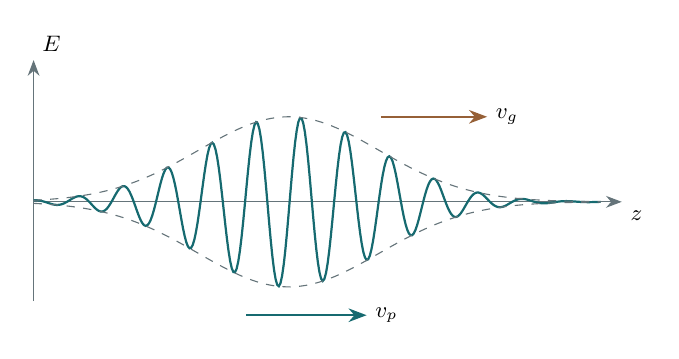
\begin{tikzpicture}[scale=.9,transform shape]
\draw[axis] (0.00000,0.00000)--(8.30000,0.00000);\draw[axis] (0.00000,-1.40000)--(0.00000,2.00000);\node[below right] at (8.30000,0.00000) {$z$};\node[above right] at (0.00000,2.00000) {$E$};\draw[traj] plot coordinates {(0.00000,0.02198) (0.02292,0.02252) (0.04585,0.02181) (0.06877,0.01976) (0.09169,0.01635) (0.11461,0.01164) (0.13754,0.00576) (0.16046,-0.00105) (0.18338,-0.00850) (0.20630,-0.01621) (0.22923,-0.02377) (0.25215,-0.03072) (0.27507,-0.03658) (0.29799,-0.04093) (0.32092,-0.04334) (0.34384,-0.04351) (0.36676,-0.04120) (0.38968,-0.03630) (0.41261,-0.02886) (0.43553,-0.01907) (0.45845,-0.00728) (0.48138,0.00603) (0.50430,0.02023) (0.52722,0.03457) (0.55014,0.04824) (0.57307,0.06041) (0.59599,0.07022) (0.61891,0.07692) (0.64183,0.07984) (0.66476,0.07849) (0.68768,0.07258) (0.71060,0.06205) (0.73352,0.04711) (0.75645,0.02824) (0.77937,0.00620) (0.80229,-0.01802) (0.82521,-0.04322) (0.84814,-0.06804) (0.87106,-0.09105) (0.89398,-0.11078) (0.91691,-0.12585) (0.93983,-0.13505) (0.96275,-0.13738) (0.98567,-0.13219) (1.00860,-0.11920) (1.03152,-0.09854) (1.05444,-0.07081) (1.07736,-0.03705) (1.10029,0.00127) (1.12321,0.04234) (1.14613,0.08402) (1.16905,0.12402) (1.19198,0.15996) (1.21490,0.18953) (1.23782,0.21063) (1.26074,0.22147) (1.28367,0.22077) (1.30659,0.20776) (1.32951,0.18236) (1.35244,0.14516) (1.37536,0.09749) (1.39828,0.04132) (1.42120,-0.02074) (1.44413,-0.08560) (1.46705,-0.14982) (1.48997,-0.20976) (1.51289,-0.26183) (1.53582,-0.30264) (1.55874,-0.32923) (1.58166,-0.33929) (1.60458,-0.33128) (1.62751,-0.30460) (1.65043,-0.25965) (1.67335,-0.19791) (1.69628,-0.12185) (1.71920,-0.03491) (1.74212,0.05871) (1.76504,0.15416) (1.78797,0.24626) (1.81089,0.32975) (1.83381,0.39956) (1.85673,0.45113) (1.87966,0.48069) (1.90258,0.48551) (1.92550,0.46410) (1.94842,0.41638) (1.97135,0.34371) (1.99427,0.24891) (2.01719,0.13618) (2.04011,0.01088) (2.06304,-0.12067) (2.08596,-0.25152) (2.10888,-0.37445) (2.13181,-0.48238) (2.15473,-0.56876) (2.17765,-0.62795) (2.20057,-0.65558) (2.22350,-0.64888) (2.24642,-0.60684) (2.26934,-0.53037) (2.29226,-0.42234) (2.31519,-0.28744) (2.33811,-0.13204) (2.36103,0.03613) (2.38395,0.20835) (2.40688,0.37538) (2.42980,0.52794) (2.45272,0.65725) (2.47564,0.75549) (2.49857,0.81631) (2.52149,0.83522) (2.54441,0.80988) (2.56734,0.74032) (2.59026,0.62901) (2.61318,0.48075) (2.63610,0.30254) (2.65903,0.10321) (2.68195,-0.10703) (2.70487,-0.31707) (2.72779,-0.51555) (2.75072,-0.69145) (2.77364,-0.83468) (2.79656,-0.93675) (2.81948,-0.99117) (2.84241,-0.99394) (2.86533,-0.94378) (2.88825,-0.84228) (2.91117,-0.69384) (2.93410,-0.50554) (2.95702,-0.28675) (2.97994,-0.04869) (3.00287,0.19617) (3.02579,0.43478) (3.04871,0.65420) (3.07163,0.84233) (3.09456,0.98858) (3.11748,1.08448) (3.14040,1.12418) (3.16332,1.10480) (3.18625,1.02663) (3.20917,0.89316) (3.23209,0.71090) (3.25501,0.48911) (3.27794,0.23926) (3.30086,-0.02553) (3.32378,-0.29122) (3.34670,-0.54361) (3.36963,-0.76909) (3.39255,-0.95543) (3.41547,-1.09242) (3.43840,-1.17248) (3.46132,-1.19105) (3.48424,-1.14688) (3.50716,-1.04210) (3.53009,-0.88212) (3.55301,-0.67536) (3.57593,-0.43275) (3.59885,-0.16719) (3.62178,0.10718) (3.64470,0.37574) (3.66762,0.62420) (3.69054,0.83936) (3.71347,1.00984) (3.73639,1.12672) (3.75931,1.18396) (3.78223,1.17875) (3.80516,1.11169) (3.82808,0.98667) (3.85100,0.81068) (3.87393,0.59341) (3.89685,0.34670) (3.91977,0.08388) (3.94269,-0.18098) (3.96562,-0.43379) (3.98854,-0.66128) (4.01146,-0.85165) (4.03438,-0.99522) (4.05731,-1.08494) (4.08023,-1.11673) (4.10315,-1.08966) (4.12607,-1.00598) (4.14900,-0.87093) (4.17192,-0.69242) (4.19484,-0.48059) (4.21777,-0.24717) (4.24069,-0.00489) (4.26361,0.23330) (4.28653,0.45487) (4.30946,0.64842) (4.33238,0.80428) (4.35530,0.91496) (4.37822,0.97555) (4.40115,0.98393) (4.42407,0.94079) (4.44699,0.84958) (4.46991,0.71623) (4.49284,0.54877) (4.51576,0.35689) (4.53868,0.15132) (4.56160,-0.05675) (4.58453,-0.25628) (4.60745,-0.43697) (4.63037,-0.58982) (4.65330,-0.70757) (4.67622,-0.78501) (4.69914,-0.81926) (4.72206,-0.80981) (4.74499,-0.75851) (4.76791,-0.66937) (4.79083,-0.54829) (4.81375,-0.40270) (4.83668,-0.24107) (4.85960,-0.07246) (4.88252,0.09401) (4.90544,0.24966) (4.92837,0.38668) (4.95129,0.49854) (4.97421,0.58028) (4.99713,0.62874) (5.02006,0.64263) (5.04298,0.62257) (5.06590,0.57096) (5.08883,0.49177) (5.11175,0.39029) (5.13467,0.27278) (5.15759,0.14609) (5.18052,0.01727) (5.20344,-0.10681) (5.22636,-0.21984) (5.24928,-0.31636) (5.27221,-0.39205) (5.29513,-0.44387) (5.31805,-0.47021) (5.34097,-0.47087) (5.36390,-0.44704) (5.38682,-0.40116) (5.40974,-0.33670) (5.43266,-0.25797) (5.45559,-0.16982) (5.47851,-0.07736) (5.50143,0.01433) (5.52436,0.10047) (5.54728,0.17683) (5.57020,0.23991) (5.59312,0.28711) (5.61605,0.31681) (5.63897,0.32840) (5.66189,0.32229) (5.68481,0.29978) (5.70774,0.26299) (5.73066,0.21467) (5.75358,0.15802) (5.77650,0.09651) (5.79943,0.03367) (5.82235,-0.02714) (5.84527,-0.08282) (5.86819,-0.13078) (5.89112,-0.16896) (5.91404,-0.19596) (5.93696,-0.21106) (5.95989,-0.21423) (5.98281,-0.20606) (6.00573,-0.18770) (6.02865,-0.16080) (6.05158,-0.12732) (6.07450,-0.08947) (6.09742,-0.04952) (6.12034,-0.00973) (6.14327,0.02783) (6.16619,0.06134) (6.18911,0.08931) (6.21203,0.11065) (6.23496,0.12472) (6.25788,0.13128) (6.28080,0.13054) (6.30372,0.12305) (6.32665,0.10971) (6.34957,0.09165) (6.37249,0.07017) (6.39542,0.04665) (6.41834,0.02249) (6.44126,-0.00099) (6.46418,-0.02260) (6.48711,-0.04135) (6.51003,-0.05648) (6.53295,-0.06746) (6.55587,-0.07406) (6.57880,-0.07626) (6.60172,-0.07430) (6.62464,-0.06863) (6.64756,-0.05984) (6.67049,-0.04866) (6.69341,-0.03586) (6.71633,-0.02227) (6.73926,-0.00866) (6.76218,0.00425) (6.78510,0.01582) (6.80802,0.02558) (6.83095,0.03315) (6.85387,0.03832) (6.87679,0.04104) (6.89971,0.04137) (6.92264,0.03951) (6.94556,0.03574) (6.96848,0.03045) (6.99140,0.02404) (7.01433,0.01696) (7.03725,0.00965) (7.06017,0.00250) (7.08309,-0.00410) (7.10602,-0.00988) (7.12894,-0.01459) (7.15186,-0.01808) (7.17479,-0.02030) (7.19771,-0.02123) (7.22063,-0.02096) (7.24355,-0.01962) (7.26648,-0.01738) (7.28940,-0.01445) (7.31232,-0.01104) (7.33524,-0.00740) (7.35817,-0.00373) (7.38109,-0.00024) (7.40401,0.00291) (7.42693,0.00559) (7.44986,0.00769) (7.47278,0.00918) (7.49570,0.01003) (7.51862,0.01026) (7.54155,0.00992) (7.56447,0.00910) (7.58739,0.00789) (7.61032,0.00639) (7.63324,0.00471) (7.65616,0.00296) (7.67908,0.00125) (7.70201,-0.00034) (7.72493,-0.00174) (7.74785,-0.00289) (7.77077,-0.00376) (7.79370,-0.00434) (7.81662,-0.00462) (7.83954,-0.00463) (7.86246,-0.00439) (7.88539,-0.00394) (7.90831,-0.00334) (7.93123,-0.00263) (7.95415,-0.00186) (7.97708,-0.00108) (8.00000,-0.00034)};\draw[guide] plot coordinates {(0.00000,0.02198) (0.02292,0.02312) (0.04585,0.02432) (0.06877,0.02557) (0.09169,0.02688) (0.11461,0.02824) (0.13754,0.02966) (0.16046,0.03115) (0.18338,0.03269) (0.20630,0.03431) (0.22923,0.03599) (0.25215,0.03774) (0.27507,0.03957) (0.29799,0.04147) (0.32092,0.04344) (0.34384,0.04550) (0.36676,0.04764) (0.38968,0.04986) (0.41261,0.05217) (0.43553,0.05456) (0.45845,0.05705) (0.48138,0.05964) (0.50430,0.06232) (0.52722,0.06510) (0.55014,0.06798) (0.57307,0.07097) (0.59599,0.07406) (0.61891,0.07726) (0.64183,0.08058) (0.66476,0.08401) (0.68768,0.08756) (0.71060,0.09123) (0.73352,0.09502) (0.75645,0.09893) (0.77937,0.10298) (0.80229,0.10716) (0.82521,0.11146) (0.84814,0.11591) (0.87106,0.12049) (0.89398,0.12522) (0.91691,0.13008) (0.93983,0.13509) (0.96275,0.14025) (0.98567,0.14556) (1.00860,0.15102) (1.03152,0.15664) (1.05444,0.16241) (1.07736,0.16834) (1.10029,0.17443) (1.12321,0.18068) (1.14613,0.18709) (1.16905,0.19367) (1.19198,0.20042) (1.21490,0.20733) (1.23782,0.21441) (1.26074,0.22166) (1.28367,0.22908) (1.30659,0.23668) (1.32951,0.24445) (1.35244,0.25239) (1.37536,0.26050) (1.39828,0.26879) (1.42120,0.27725) (1.44413,0.28588) (1.46705,0.29469) (1.48997,0.30367) (1.51289,0.31282) (1.53582,0.32214) (1.55874,0.33164) (1.58166,0.34130) (1.60458,0.35113) (1.62751,0.36113) (1.65043,0.37129) (1.67335,0.38161) (1.69628,0.39210) (1.71920,0.40274) (1.74212,0.41353) (1.76504,0.42448) (1.78797,0.43557) (1.81089,0.44681) (1.83381,0.45819) (1.85673,0.46971) (1.87966,0.48136) (1.90258,0.49315) (1.92550,0.50505) (1.94842,0.51708) (1.97135,0.52922) (1.99427,0.54147) (2.01719,0.55382) (2.04011,0.56627) (2.06304,0.57882) (2.08596,0.59145) (2.10888,0.60416) (2.13181,0.61694) (2.15473,0.62979) (2.17765,0.64269) (2.20057,0.65565) (2.22350,0.66866) (2.24642,0.68170) (2.26934,0.69477) (2.29226,0.70786) (2.31519,0.72096) (2.33811,0.73407) (2.36103,0.74717) (2.38395,0.76027) (2.40688,0.77333) (2.42980,0.78637) (2.45272,0.79937) (2.47564,0.81232) (2.49857,0.82522) (2.52149,0.83804) (2.54441,0.85079) (2.56734,0.86346) (2.59026,0.87602) (2.61318,0.88848) (2.63610,0.90083) (2.65903,0.91305) (2.68195,0.92514) (2.70487,0.93709) (2.72779,0.94888) (2.75072,0.96050) (2.77364,0.97196) (2.79656,0.98323) (2.81948,0.99431) (2.84241,1.00519) (2.86533,1.01586) (2.88825,1.02631) (2.91117,1.03653) (2.93410,1.04651) (2.95702,1.05625) (2.97994,1.06573) (3.00287,1.07494) (3.02579,1.08389) (3.04871,1.09256) (3.07163,1.10093) (3.09456,1.10901) (3.11748,1.11679) (3.14040,1.12426) (3.16332,1.13141) (3.18625,1.13824) (3.20917,1.14474) (3.23209,1.15090) (3.25501,1.15672) (3.27794,1.16219) (3.30086,1.16731) (3.32378,1.17207) (3.34670,1.17647) (3.36963,1.18050) (3.39255,1.18417) (3.41547,1.18745) (3.43840,1.19037) (3.46132,1.19290) (3.48424,1.19505) (3.50716,1.19681) (3.53009,1.19819) (3.55301,1.19918) (3.57593,1.19979) (3.59885,1.20000) (3.62178,1.19982) (3.64470,1.19926) (3.66762,1.19831) (3.69054,1.19697) (3.71347,1.19524) (3.73639,1.19313) (3.75931,1.19064) (3.78223,1.18776) (3.80516,1.18451) (3.82808,1.18089) (3.85100,1.17689) (3.87393,1.17253) (3.89685,1.16780) (3.91977,1.16272) (3.94269,1.15728) (3.96562,1.15150) (3.98854,1.14537) (4.01146,1.13891) (4.03438,1.13211) (4.05731,1.12499) (4.08023,1.11755) (4.10315,1.10981) (4.12607,1.10175) (4.14900,1.09341) (4.17192,1.08477) (4.19484,1.07585) (4.21777,1.06666) (4.24069,1.05721) (4.26361,1.04750) (4.28653,1.03754) (4.30946,1.02734) (4.33238,1.01691) (4.35530,1.00627) (4.37822,0.99541) (4.40115,0.98435) (4.42407,0.97309) (4.44699,0.96166) (4.46991,0.95005) (4.49284,0.93827) (4.51576,0.92634) (4.53868,0.91427) (4.56160,0.90206) (4.58453,0.88972) (4.60745,0.87727) (4.63037,0.86472) (4.65330,0.85206) (4.67622,0.83932) (4.69914,0.82650) (4.72206,0.81362) (4.74499,0.80067) (4.76791,0.78768) (4.79083,0.77464) (4.81375,0.76157) (4.83668,0.74848) (4.85960,0.73538) (4.88252,0.72227) (4.90544,0.70917) (4.92837,0.69608) (4.95129,0.68300) (4.97421,0.66996) (4.99713,0.65695) (5.02006,0.64399) (5.04298,0.63108) (5.06590,0.61822) (5.08883,0.60543) (5.11175,0.59271) (5.13467,0.58008) (5.15759,0.56752) (5.18052,0.55506) (5.20344,0.54270) (5.22636,0.53044) (5.24928,0.51829) (5.27221,0.50625) (5.29513,0.49433) (5.31805,0.48254) (5.34097,0.47087) (5.36390,0.45934) (5.38682,0.44794) (5.40974,0.43669) (5.43266,0.42558) (5.45559,0.41462) (5.47851,0.40381) (5.50143,0.39315) (5.52436,0.38265) (5.54728,0.37231) (5.57020,0.36214) (5.59312,0.35212) (5.61605,0.34228) (5.63897,0.33260) (5.66189,0.32309) (5.68481,0.31374) (5.70774,0.30458) (5.73066,0.29558) (5.75358,0.28675) (5.77650,0.27810) (5.79943,0.26962) (5.82235,0.26132) (5.84527,0.25319) (5.86819,0.24523) (5.89112,0.23745) (5.91404,0.22984) (5.93696,0.22240) (5.95989,0.21513) (5.98281,0.20803) (6.00573,0.20110) (6.02865,0.19434) (6.05158,0.18774) (6.07450,0.18131) (6.09742,0.17504) (6.12034,0.16894) (6.14327,0.16299) (6.16619,0.15721) (6.18911,0.15158) (6.21203,0.14610) (6.23496,0.14078) (6.25788,0.13560) (6.28080,0.13058) (6.30372,0.12570) (6.32665,0.12096) (6.34957,0.11636) (6.37249,0.11190) (6.39542,0.10758) (6.41834,0.10339) (6.44126,0.09933) (6.46418,0.09540) (6.48711,0.09160) (6.51003,0.08792) (6.53295,0.08436) (6.55587,0.08092) (6.57880,0.07759) (6.60172,0.07437) (6.62464,0.07127) (6.64756,0.06827) (6.67049,0.06538) (6.69341,0.06259) (6.71633,0.05990) (6.73926,0.05731) (6.76218,0.05481) (6.78510,0.05240) (6.80802,0.05008) (6.83095,0.04785) (6.85387,0.04571) (6.87679,0.04364) (6.89971,0.04166) (6.92264,0.03975) (6.94556,0.03792) (6.96848,0.03616) (6.99140,0.03447) (7.01433,0.03285) (7.03725,0.03130) (7.06017,0.02981) (7.08309,0.02838) (7.10602,0.02701) (7.12894,0.02570) (7.15186,0.02444) (7.17479,0.02324) (7.19771,0.02209) (7.22063,0.02099) (7.24355,0.01994) (7.26648,0.01893) (7.28940,0.01797) (7.31232,0.01706) (7.33524,0.01618) (7.35817,0.01535) (7.38109,0.01455) (7.40401,0.01379) (7.42693,0.01306) (7.44986,0.01237) (7.47278,0.01172) (7.49570,0.01109) (7.51862,0.01049) (7.54155,0.00993) (7.56447,0.00939) (7.58739,0.00887) (7.61032,0.00838) (7.63324,0.00792) (7.65616,0.00748) (7.67908,0.00706) (7.70201,0.00666) (7.72493,0.00629) (7.74785,0.00593) (7.77077,0.00559) (7.79370,0.00527) (7.81662,0.00497) (7.83954,0.00468) (7.86246,0.00440) (7.88539,0.00415) (7.90831,0.00390) (7.93123,0.00367) (7.95415,0.00345) (7.97708,0.00324) (8.00000,0.00305)};\draw[guide] plot coordinates {(0.00000,-0.02198) (0.02292,-0.02312) (0.04585,-0.02432) (0.06877,-0.02557) (0.09169,-0.02688) (0.11461,-0.02824) (0.13754,-0.02966) (0.16046,-0.03115) (0.18338,-0.03269) (0.20630,-0.03431) (0.22923,-0.03599) (0.25215,-0.03774) (0.27507,-0.03957) (0.29799,-0.04147) (0.32092,-0.04344) (0.34384,-0.04550) (0.36676,-0.04764) (0.38968,-0.04986) (0.41261,-0.05217) (0.43553,-0.05456) (0.45845,-0.05705) (0.48138,-0.05964) (0.50430,-0.06232) (0.52722,-0.06510) (0.55014,-0.06798) (0.57307,-0.07097) (0.59599,-0.07406) (0.61891,-0.07726) (0.64183,-0.08058) (0.66476,-0.08401) (0.68768,-0.08756) (0.71060,-0.09123) (0.73352,-0.09502) (0.75645,-0.09893) (0.77937,-0.10298) (0.80229,-0.10716) (0.82521,-0.11146) (0.84814,-0.11591) (0.87106,-0.12049) (0.89398,-0.12522) (0.91691,-0.13008) (0.93983,-0.13509) (0.96275,-0.14025) (0.98567,-0.14556) (1.00860,-0.15102) (1.03152,-0.15664) (1.05444,-0.16241) (1.07736,-0.16834) (1.10029,-0.17443) (1.12321,-0.18068) (1.14613,-0.18709) (1.16905,-0.19367) (1.19198,-0.20042) (1.21490,-0.20733) (1.23782,-0.21441) (1.26074,-0.22166) (1.28367,-0.22908) (1.30659,-0.23668) (1.32951,-0.24445) (1.35244,-0.25239) (1.37536,-0.26050) (1.39828,-0.26879) (1.42120,-0.27725) (1.44413,-0.28588) (1.46705,-0.29469) (1.48997,-0.30367) (1.51289,-0.31282) (1.53582,-0.32214) (1.55874,-0.33164) (1.58166,-0.34130) (1.60458,-0.35113) (1.62751,-0.36113) (1.65043,-0.37129) (1.67335,-0.38161) (1.69628,-0.39210) (1.71920,-0.40274) (1.74212,-0.41353) (1.76504,-0.42448) (1.78797,-0.43557) (1.81089,-0.44681) (1.83381,-0.45819) (1.85673,-0.46971) (1.87966,-0.48136) (1.90258,-0.49315) (1.92550,-0.50505) (1.94842,-0.51708) (1.97135,-0.52922) (1.99427,-0.54147) (2.01719,-0.55382) (2.04011,-0.56627) (2.06304,-0.57882) (2.08596,-0.59145) (2.10888,-0.60416) (2.13181,-0.61694) (2.15473,-0.62979) (2.17765,-0.64269) (2.20057,-0.65565) (2.22350,-0.66866) (2.24642,-0.68170) (2.26934,-0.69477) (2.29226,-0.70786) (2.31519,-0.72096) (2.33811,-0.73407) (2.36103,-0.74717) (2.38395,-0.76027) (2.40688,-0.77333) (2.42980,-0.78637) (2.45272,-0.79937) (2.47564,-0.81232) (2.49857,-0.82522) (2.52149,-0.83804) (2.54441,-0.85079) (2.56734,-0.86346) (2.59026,-0.87602) (2.61318,-0.88848) (2.63610,-0.90083) (2.65903,-0.91305) (2.68195,-0.92514) (2.70487,-0.93709) (2.72779,-0.94888) (2.75072,-0.96050) (2.77364,-0.97196) (2.79656,-0.98323) (2.81948,-0.99431) (2.84241,-1.00519) (2.86533,-1.01586) (2.88825,-1.02631) (2.91117,-1.03653) (2.93410,-1.04651) (2.95702,-1.05625) (2.97994,-1.06573) (3.00287,-1.07494) (3.02579,-1.08389) (3.04871,-1.09256) (3.07163,-1.10093) (3.09456,-1.10901) (3.11748,-1.11679) (3.14040,-1.12426) (3.16332,-1.13141) (3.18625,-1.13824) (3.20917,-1.14474) (3.23209,-1.15090) (3.25501,-1.15672) (3.27794,-1.16219) (3.30086,-1.16731) (3.32378,-1.17207) (3.34670,-1.17647) (3.36963,-1.18050) (3.39255,-1.18417) (3.41547,-1.18745) (3.43840,-1.19037) (3.46132,-1.19290) (3.48424,-1.19505) (3.50716,-1.19681) (3.53009,-1.19819) (3.55301,-1.19918) (3.57593,-1.19979) (3.59885,-1.20000) (3.62178,-1.19982) (3.64470,-1.19926) (3.66762,-1.19831) (3.69054,-1.19697) (3.71347,-1.19524) (3.73639,-1.19313) (3.75931,-1.19064) (3.78223,-1.18776) (3.80516,-1.18451) (3.82808,-1.18089) (3.85100,-1.17689) (3.87393,-1.17253) (3.89685,-1.16780) (3.91977,-1.16272) (3.94269,-1.15728) (3.96562,-1.15150) (3.98854,-1.14537) (4.01146,-1.13891) (4.03438,-1.13211) (4.05731,-1.12499) (4.08023,-1.11755) (4.10315,-1.10981) (4.12607,-1.10175) (4.14900,-1.09341) (4.17192,-1.08477) (4.19484,-1.07585) (4.21777,-1.06666) (4.24069,-1.05721) (4.26361,-1.04750) (4.28653,-1.03754) (4.30946,-1.02734) (4.33238,-1.01691) (4.35530,-1.00627) (4.37822,-0.99541) (4.40115,-0.98435) (4.42407,-0.97309) (4.44699,-0.96166) (4.46991,-0.95005) (4.49284,-0.93827) (4.51576,-0.92634) (4.53868,-0.91427) (4.56160,-0.90206) (4.58453,-0.88972) (4.60745,-0.87727) (4.63037,-0.86472) (4.65330,-0.85206) (4.67622,-0.83932) (4.69914,-0.82650) (4.72206,-0.81362) (4.74499,-0.80067) (4.76791,-0.78768) (4.79083,-0.77464) (4.81375,-0.76157) (4.83668,-0.74848) (4.85960,-0.73538) (4.88252,-0.72227) (4.90544,-0.70917) (4.92837,-0.69608) (4.95129,-0.68300) (4.97421,-0.66996) (4.99713,-0.65695) (5.02006,-0.64399) (5.04298,-0.63108) (5.06590,-0.61822) (5.08883,-0.60543) (5.11175,-0.59271) (5.13467,-0.58008) (5.15759,-0.56752) (5.18052,-0.55506) (5.20344,-0.54270) (5.22636,-0.53044) (5.24928,-0.51829) (5.27221,-0.50625) (5.29513,-0.49433) (5.31805,-0.48254) (5.34097,-0.47087) (5.36390,-0.45934) (5.38682,-0.44794) (5.40974,-0.43669) (5.43266,-0.42558) (5.45559,-0.41462) (5.47851,-0.40381) (5.50143,-0.39315) (5.52436,-0.38265) (5.54728,-0.37231) (5.57020,-0.36214) (5.59312,-0.35212) (5.61605,-0.34228) (5.63897,-0.33260) (5.66189,-0.32309) (5.68481,-0.31374) (5.70774,-0.30458) (5.73066,-0.29558) (5.75358,-0.28675) (5.77650,-0.27810) (5.79943,-0.26962) (5.82235,-0.26132) (5.84527,-0.25319) (5.86819,-0.24523) (5.89112,-0.23745) (5.91404,-0.22984) (5.93696,-0.22240) (5.95989,-0.21513) (5.98281,-0.20803) (6.00573,-0.20110) (6.02865,-0.19434) (6.05158,-0.18774) (6.07450,-0.18131) (6.09742,-0.17504) (6.12034,-0.16894) (6.14327,-0.16299) (6.16619,-0.15721) (6.18911,-0.15158) (6.21203,-0.14610) (6.23496,-0.14078) (6.25788,-0.13560) (6.28080,-0.13058) (6.30372,-0.12570) (6.32665,-0.12096) (6.34957,-0.11636) (6.37249,-0.11190) (6.39542,-0.10758) (6.41834,-0.10339) (6.44126,-0.09933) (6.46418,-0.09540) (6.48711,-0.09160) (6.51003,-0.08792) (6.53295,-0.08436) (6.55587,-0.08092) (6.57880,-0.07759) (6.60172,-0.07437) (6.62464,-0.07127) (6.64756,-0.06827) (6.67049,-0.06538) (6.69341,-0.06259) (6.71633,-0.05990) (6.73926,-0.05731) (6.76218,-0.05481) (6.78510,-0.05240) (6.80802,-0.05008) (6.83095,-0.04785) (6.85387,-0.04571) (6.87679,-0.04364) (6.89971,-0.04166) (6.92264,-0.03975) (6.94556,-0.03792) (6.96848,-0.03616) (6.99140,-0.03447) (7.01433,-0.03285) (7.03725,-0.03130) (7.06017,-0.02981) (7.08309,-0.02838) (7.10602,-0.02701) (7.12894,-0.02570) (7.15186,-0.02444) (7.17479,-0.02324) (7.19771,-0.02209) (7.22063,-0.02099) (7.24355,-0.01994) (7.26648,-0.01893) (7.28940,-0.01797) (7.31232,-0.01706) (7.33524,-0.01618) (7.35817,-0.01535) (7.38109,-0.01455) (7.40401,-0.01379) (7.42693,-0.01306) (7.44986,-0.01237) (7.47278,-0.01172) (7.49570,-0.01109) (7.51862,-0.01049) (7.54155,-0.00993) (7.56447,-0.00939) (7.58739,-0.00887) (7.61032,-0.00838) (7.63324,-0.00792) (7.65616,-0.00748) (7.67908,-0.00706) (7.70201,-0.00666) (7.72493,-0.00629) (7.74785,-0.00593) (7.77077,-0.00559) (7.79370,-0.00527) (7.81662,-0.00497) (7.83954,-0.00468) (7.86246,-0.00440) (7.88539,-0.00415) (7.90831,-0.00390) (7.93123,-0.00367) (7.95415,-0.00345) (7.97708,-0.00324) (8.00000,-0.00305)};\draw[force] (4.90000,1.20000)--(6.40000,1.20000);\node[right] at (6.40000,1.20000) {$v_g$};\draw[motion] (3.00000,-1.60000)--(4.70000,-1.60000);\node[right] at (4.70000,-1.60000) {$v_p$};
\end{tikzpicture}
\figcaption{图光5.1\quad 载波与外包络具有不同的传播速度。}
\end{minipage}\end{center}

\Needspace{8\baselineskip}

\pdfbookmark[3]{题型定位}{q1-h0}

\subsection*{题型定位}

同一色散关系的割线斜率和切线斜率分别给相速与群速。先固定波长自变量，再求导数、说明局部折射率校准，最后区分完整分母与弱色散一次式。图中包络、色散曲线和数值速度沿同一条推导相连。

\Needspace{8\baselineskip}

\pdfbookmark[3]{知识点}{q1-h1}

\subsection*{知识点}

\begin{itemize}
\item 固定相位面的速度为$\omega/k$，窄带包络的一次相位差给$\dd\omega/\dd k$。
\item 真空波长满足$\lambda_0\omega=2\pi c$，介质内波长满足$\lambda_mk=2\pi$，求导时通过链式关系转换。
\item 真空波长形式的群折射率为$n_g=n-\lambda_0n'$；弱色散一次速度式的相对误差为$\eta^2$。
\item 常数项校准保持色散斜率，同时改变$n,n_g$与两种速度；两组数值按各自一致的折射率处理。
\end{itemize}

\Needspace{8\baselineskip}

\pdfbookmark[3]{物理图像}{q1-h2}

\subsection*{物理图像}

图光5.1中波峰和包络分别标速度。解图A使用校准柯西式的实际色散曲线，原点割线、工作点切线对应两速度；B给$n_g-n$，C给两速度差，D给一次近似的误差。两斜率在本题只差约1.36\%，配合B、C的纵轴范围观察更清楚。

\Needspace{8\baselineskip}

\pdfbookmark[3]{解题入口}{q1-h3}

\subsection*{解题入口}

从$k=n\omega/c$求$\dd k/\dd\omega$，用$\omega\dd n/\dd\omega=-\lambda_0n'$转换自变量。在589.3nm处先明确采用$n_D$校准常数项，导数仍由$B,C$给出。波长用nm时，导数用每nm，先形成无量纲的$\lambda_0n'$再代速度。

\Needspace{8\baselineskip}

\pdfbookmark[3]{标准解法}{q1-h4}

\subsection*{标准解法}


图光5.1的细密波峰表示载波相位，虚线包络表示相邻频率分量叠加后的振幅。用真空波长$\lambda_0$表示题给色散，介质内波长记为$\lambda_m$，二者分别满足$\lambda_0\omega=2\pi c$、$\lambda_mk=2\pi$。先把两种速度都写在同一条$k(\omega)$色散关系上：
\[
k(\omega)=\frac{n(\omega)\omega}{c},\quad
v_p=\frac{\omega}{k}=\frac cn,\quad
\frac1{v_g}=\frac{\dd k}{\dd\omega}=\frac1c\left(n+\omega\frac{\dd n}{\dd\omega}\right).
\]
窄带波包可把$k(\omega)$在中心频率展开到一次，包络沿$z-v_gt$移动。由$\dd\lambda_0/\dd\omega=-\lambda_0/\omega$，有$\omega\,\dd n/\dd\omega=-\lambda_0\,\dd n/\dd\lambda_0$，因此
\[
n_g=n-\lambda_0 n',\qquad \boxed{v_g=\frac c{n-\lambda_0 n'}}.
\]
下面把题给$n_D$作为589.3nm处的局部折射率，并保留柯西式给定的斜率。具体做法是先算$n_{\rm fit}(589.3)=1.51562655$，与$n_D=1.51630$相差$\Delta A=.0006734503$，再把常数项校准为$A_c=A+\Delta A=1.5046734503$。校准式$n_c(\lambda_0)=A_c+B/\lambda_0^2+C/\lambda_0^4$在589.3nm处取$n_D$，导数仍由$B,C$给出：$n'=-2B/\lambda_0^3-4C/\lambda_0^5$。

在$\lambda_0=589.3\,\mathrm{nm}$处，用nm作为求导长度单位，有
\[
n'=-3.55556\times10^{-5}\,\mathrm{nm^{-1}},\qquad
-\lambda_0 n'=0.0209529.
\]
其中$n'$的单位为$\mathrm{nm^{-1}}$，与以nm写的$\lambda_0$相乘后无量纲。解图光5.1B画出校准后的$n_c$与$n_g$；在所示可见光区间$n'<0$，所以$n_g-n=-\lambda_0n'>0$。
\begin{center}\begin{minipage}{.98\linewidth}\centering
\begin{tikzpicture}[scale=.88,transform shape]
\draw[axis] (0,0)--(7.3,0) node[right] {$\lambda_0/{\rm nm}$};
\draw[axis] (0,0)--(0,2.8);
\node[above left] at (0,2.8) {$\text{折射率}$};
\draw[thin] (0.000000,0)--(0.000000,-0.06);\node[below,font=\scriptsize] at (0.000000,-0.08) {$ 420 $};
\draw[thin] (1.473684,0)--(1.473684,-0.06);\node[below,font=\scriptsize] at (1.473684,-0.08) {$ 500 $};
\draw[thin] (3.118684,0)--(3.118684,-0.06);\node[below,font=\scriptsize] at (3.118684,-0.08) {$ 589.3 $};
\draw[thin] (5.157895,0)--(5.157895,-0.06);\node[below,font=\scriptsize] at (5.157895,-0.08) {$ 700 $};
\draw[thin] (7.000000,0)--(7.000000,-0.06);\node[below,font=\scriptsize] at (7.000000,-0.08) {$ 800 $};
\draw[thin] (0,0.000000)--(-.06,0.000000);\node[left,font=\scriptsize] at (-.08,0.000000) {$ 1.5 $};
\draw[thin] (0,0.625000)--(-.06,0.625000);\node[left,font=\scriptsize] at (-.08,0.625000) {$ 1.52 $};
\draw[thin] (0,1.250000)--(-.06,1.250000);\node[left,font=\scriptsize] at (-.08,1.250000) {$ 1.54 $};
\draw[thin] (0,1.875000)--(-.06,1.875000);\node[left,font=\scriptsize] at (-.08,1.875000) {$ 1.56 $};
\draw[thin] (0,2.500000)--(-.06,2.500000);\node[left,font=\scriptsize] at (-.08,2.500000) {$ 1.58 $};
\draw[thick,color=accent] plot coordinates {(0.0000000,0.7927855) (0.0291667,0.7889732) (0.0583333,0.7851882) (0.0875000,0.7814304) (0.1166667,0.7776997) (0.1458333,0.7739959) (0.1750000,0.7703190) (0.2041667,0.7666687) (0.2333333,0.7630449) (0.2625000,0.7594475) (0.2916667,0.7558764) (0.3208333,0.7523313) (0.3500000,0.7488122) (0.3791667,0.7453189) (0.4083333,0.7418512) (0.4375000,0.7384090) (0.4666667,0.7349922) (0.4958333,0.7316005) (0.5250000,0.7282338) (0.5541667,0.7248919) (0.5833333,0.7215748) (0.6125000,0.7182821) (0.6416667,0.7150138) (0.6708333,0.7117697) (0.7000000,0.7085496) (0.7291667,0.7053534) (0.7583333,0.7021808) (0.7875000,0.6990318) (0.8166667,0.6959061) (0.8458333,0.6928036) (0.8750000,0.6897241) (0.9041667,0.6866675) (0.9333333,0.6836335) (0.9625000,0.6806221) (0.9916667,0.6776330) (1.0208333,0.6746660) (1.0500000,0.6717211) (1.0791667,0.6687980) (1.1083333,0.6658966) (1.1375000,0.6630166) (1.1666667,0.6601580) (1.1958333,0.6573206) (1.2250000,0.6545042) (1.2541667,0.6517086) (1.2833333,0.6489337) (1.3125000,0.6461794) (1.3416667,0.6434453) (1.3708333,0.6407315) (1.4000000,0.6380377) (1.4291667,0.6353637) (1.4583333,0.6327094) (1.4875000,0.6300747) (1.5166667,0.6274594) (1.5458333,0.6248633) (1.5750000,0.6222863) (1.6041667,0.6197282) (1.6333333,0.6171888) (1.6625000,0.6146681) (1.6916667,0.6121658) (1.7208333,0.6096818) (1.7500000,0.6072160) (1.7791667,0.6047682) (1.8083333,0.6023382) (1.8375000,0.5999259) (1.8666667,0.5975312) (1.8958333,0.5951539) (1.9250000,0.5927938) (1.9541667,0.5904509) (1.9833333,0.5881250) (2.0125000,0.5858159) (2.0416667,0.5835234) (2.0708333,0.5812476) (2.1000000,0.5789881) (2.1291667,0.5767449) (2.1583333,0.5745179) (2.1875000,0.5723069) (2.2166667,0.5701117) (2.2458333,0.5679323) (2.2750000,0.5657685) (2.3041667,0.5636201) (2.3333333,0.5614871) (2.3625000,0.5593693) (2.3916667,0.5572666) (2.4208333,0.5551788) (2.4500000,0.5531059) (2.4791667,0.5510476) (2.5083333,0.5490040) (2.5375000,0.5469748) (2.5666667,0.5449599) (2.5958333,0.5429592) (2.6250000,0.5409727) (2.6541667,0.5390001) (2.6833333,0.5370413) (2.7125000,0.5350963) (2.7416667,0.5331650) (2.7708333,0.5312471) (2.8000000,0.5293426) (2.8291667,0.5274514) (2.8583333,0.5255733) (2.8875000,0.5237084) (2.9166667,0.5218563) (2.9458333,0.5200171) (2.9750000,0.5181906) (3.0041667,0.5163768) (3.0333333,0.5145754) (3.0625000,0.5127865) (3.0916667,0.5110098) (3.1208333,0.5092454) (3.1500000,0.5074931) (3.1791667,0.5057527) (3.2083333,0.5040243) (3.2375000,0.5023076) (3.2666667,0.5006027) (3.2958333,0.4989093) (3.3250000,0.4972274) (3.3541667,0.4955570) (3.3833333,0.4938978) (3.4125000,0.4922499) (3.4416667,0.4906131) (3.4708333,0.4889873) (3.5000000,0.4873725) (3.5291667,0.4857685) (3.5583333,0.4841752) (3.5875000,0.4825927) (3.6166667,0.4810207) (3.6458333,0.4794591) (3.6750000,0.4779080) (3.7041667,0.4763672) (3.7333333,0.4748367) (3.7625000,0.4733162) (3.7916667,0.4718059) (3.8208333,0.4703055) (3.8500000,0.4688150) (3.8791667,0.4673344) (3.9083333,0.4658634) (3.9375000,0.4644021) (3.9666667,0.4629504) (3.9958333,0.4615082) (4.0250000,0.4600754) (4.0541667,0.4586520) (4.0833333,0.4572378) (4.1125000,0.4558328) (4.1416667,0.4544369) (4.1708333,0.4530501) (4.2000000,0.4516722) (4.2291667,0.4503032) (4.2583333,0.4489431) (4.2875000,0.4475916) (4.3166667,0.4462489) (4.3458333,0.4449148) (4.3750000,0.4435892) (4.4041667,0.4422721) (4.4333333,0.4409634) (4.4625000,0.4396630) (4.4916667,0.4383709) (4.5208333,0.4370870) (4.5500000,0.4358112) (4.5791667,0.4345435) (4.6083333,0.4332838) (4.6375000,0.4320320) (4.6666667,0.4307881) (4.6958333,0.4295521) (4.7250000,0.4283238) (4.7541667,0.4271031) (4.7833333,0.4258901) (4.8125000,0.4246847) (4.8416667,0.4234868) (4.8708333,0.4222963) (4.9000000,0.4211132) (4.9291667,0.4199375) (4.9583333,0.4187690) (4.9875000,0.4176077) (5.0166667,0.4164537) (5.0458333,0.4153067) (5.0750000,0.4141667) (5.1041667,0.4130338) (5.1333333,0.4119078) (5.1625000,0.4107886) (5.1916667,0.4096763) (5.2208333,0.4085708) (5.2500000,0.4074720) (5.2791667,0.4063799) (5.3083333,0.4052944) (5.3375000,0.4042155) (5.3666667,0.4031431) (5.3958333,0.4020771) (5.4250000,0.4010176) (5.4541667,0.3999645) (5.4833333,0.3989176) (5.5125000,0.3978771) (5.5416667,0.3968427) (5.5708333,0.3958146) (5.6000000,0.3947925) (5.6291667,0.3937766) (5.6583333,0.3927667) (5.6875000,0.3917627) (5.7166667,0.3907648) (5.7458333,0.3897727) (5.7750000,0.3887864) (5.8041667,0.3878060) (5.8333333,0.3868314) (5.8625000,0.3858624) (5.8916667,0.3848992) (5.9208333,0.3839416) (5.9500000,0.3829895) (5.9791667,0.3820431) (6.0083333,0.3811021) (6.0375000,0.3801666) (6.0666667,0.3792365) (6.0958333,0.3783119) (6.1250000,0.3773925) (6.1541667,0.3764785) (6.1833333,0.3755698) (6.2125000,0.3746662) (6.2416667,0.3737679) (6.2708333,0.3728747) (6.3000000,0.3719867) (6.3291667,0.3711037) (6.3583333,0.3702257) (6.3875000,0.3693528) (6.4166667,0.3684848) (6.4458333,0.3676217) (6.4750000,0.3667635) (6.5041667,0.3659102) (6.5333333,0.3650617) (6.5625000,0.3642180) (6.5916667,0.3633791) (6.6208333,0.3625448) (6.6500000,0.3617153) (6.6791667,0.3608904) (6.7083333,0.3600701) (6.7375000,0.3592544) (6.7666667,0.3584432) (6.7958333,0.3576366) (6.8250000,0.3568344) (6.8541667,0.3560367) (6.8833333,0.3552434) (6.9125000,0.3544545) (6.9416667,0.3536699) (6.9708333,0.3528897) (7.0000000,0.3521137)};
\draw[thick,color=accent] (7.65,2.55)--(8.15,2.55);\node[right,font=\scriptsize] at (8.2,2.55) {$n$};
\draw[thick,dashed,color=warm] plot coordinates {(0.0000000,1.8076798) (0.0291667,1.8004045) (0.0583333,1.7931337) (0.0875000,1.7858689) (0.1166667,1.7786112) (0.1458333,1.7713620) (0.1750000,1.7641223) (0.2041667,1.7568935) (0.2333333,1.7496765) (0.2625000,1.7424724) (0.2916667,1.7352822) (0.3208333,1.7281068) (0.3500000,1.7209473) (0.3791667,1.7138044) (0.4083333,1.7066790) (0.4375000,1.6995719) (0.4666667,1.6924838) (0.4958333,1.6854155) (0.5250000,1.6783677) (0.5541667,1.6713409) (0.5833333,1.6643360) (0.6125000,1.6573534) (0.6416667,1.6503937) (0.6708333,1.6434575) (0.7000000,1.6365453) (0.7291667,1.6296575) (0.7583333,1.6227947) (0.7875000,1.6159573) (0.8166667,1.6091456) (0.8458333,1.6023601) (0.8750000,1.5956012) (0.9041667,1.5888692) (0.9333333,1.5821644) (0.9625000,1.5754871) (0.9916667,1.5688377) (1.0208333,1.5622164) (1.0500000,1.5556235) (1.0791667,1.5490591) (1.1083333,1.5425236) (1.1375000,1.5360172) (1.1666667,1.5295400) (1.1958333,1.5230922) (1.2250000,1.5166740) (1.2541667,1.5102855) (1.2833333,1.5039269) (1.3125000,1.4975983) (1.3416667,1.4912999) (1.3708333,1.4850316) (1.4000000,1.4787937) (1.4291667,1.4725862) (1.4583333,1.4664091) (1.4875000,1.4602626) (1.5166667,1.4541467) (1.5458333,1.4480614) (1.5750000,1.4420068) (1.6041667,1.4359829) (1.6333333,1.4299897) (1.6625000,1.4240272) (1.6916667,1.4180955) (1.7208333,1.4121945) (1.7500000,1.4063242) (1.7791667,1.4004846) (1.8083333,1.3946757) (1.8375000,1.3888975) (1.8666667,1.3831499) (1.8958333,1.3774328) (1.9250000,1.3717463) (1.9541667,1.3660903) (1.9833333,1.3604647) (2.0125000,1.3548695) (2.0416667,1.3493045) (2.0708333,1.3437698) (2.1000000,1.3382653) (2.1291667,1.3327909) (2.1583333,1.3273464) (2.1875000,1.3219319) (2.2166667,1.3165472) (2.2458333,1.3111923) (2.2750000,1.3058669) (2.3041667,1.3005712) (2.3333333,1.2953049) (2.3625000,1.2900679) (2.3916667,1.2848602) (2.4208333,1.2796816) (2.4500000,1.2745320) (2.4791667,1.2694114) (2.5083333,1.2643195) (2.5375000,1.2592563) (2.5666667,1.2542217) (2.5958333,1.2492155) (2.6250000,1.2442377) (2.6541667,1.2392880) (2.6833333,1.2343664) (2.7125000,1.2294727) (2.7416667,1.2246069) (2.7708333,1.2197687) (2.8000000,1.2149581) (2.8291667,1.2101750) (2.8583333,1.2054191) (2.8875000,1.2006904) (2.9166667,1.1959887) (2.9458333,1.1913139) (2.9750000,1.1866658) (3.0041667,1.1820444) (3.0333333,1.1774494) (3.0625000,1.1728808) (3.0916667,1.1683384) (3.1208333,1.1638220) (3.1500000,1.1593316) (3.1791667,1.1548670) (3.2083333,1.1504280) (3.2375000,1.1460145) (3.2666667,1.1416264) (3.2958333,1.1372635) (3.3250000,1.1329257) (3.3541667,1.1286128) (3.3833333,1.1243248) (3.4125000,1.1200614) (3.4416667,1.1158225) (3.4708333,1.1116080) (3.5000000,1.1074177) (3.5291667,1.1032516) (3.5583333,1.0991094) (3.5875000,1.0949910) (3.6166667,1.0908963) (3.6458333,1.0868251) (3.6750000,1.0827774) (3.7041667,1.0787529) (3.7333333,1.0747515) (3.7625000,1.0707731) (3.7916667,1.0668175) (3.8208333,1.0628846) (3.8500000,1.0589743) (3.8791667,1.0550864) (3.9083333,1.0512208) (3.9375000,1.0473774) (3.9666667,1.0435560) (3.9958333,1.0397564) (4.0250000,1.0359786) (4.0541667,1.0322224) (4.0833333,1.0284877) (4.1125000,1.0247743) (4.1416667,1.0210822) (4.1708333,1.0174111) (4.2000000,1.0137609) (4.2291667,1.0101316) (4.2583333,1.0065229) (4.2875000,1.0029348) (4.3166667,0.9993671) (4.3458333,0.9958197) (4.3750000,0.9922924) (4.4041667,0.9887852) (4.4333333,0.9852979) (4.4625000,0.9818303) (4.4916667,0.9783824) (4.5208333,0.9749540) (4.5500000,0.9715451) (4.5791667,0.9681554) (4.6083333,0.9647848) (4.6375000,0.9614333) (4.6666667,0.9581006) (4.6958333,0.9547868) (4.7250000,0.9514916) (4.7541667,0.9482149) (4.7833333,0.9449567) (4.8125000,0.9417167) (4.8416667,0.9384950) (4.8708333,0.9352913) (4.9000000,0.9321055) (4.9291667,0.9289376) (4.9583333,0.9257873) (4.9875000,0.9226547) (5.0166667,0.9195396) (5.0458333,0.9164418) (5.0750000,0.9133613) (5.1041667,0.9102979) (5.1333333,0.9072515) (5.1625000,0.9042221) (5.1916667,0.9012094) (5.2208333,0.8982135) (5.2500000,0.8952341) (5.2791667,0.8922712) (5.3083333,0.8893247) (5.3375000,0.8863945) (5.3666667,0.8834804) (5.3958333,0.8805824) (5.4250000,0.8777003) (5.4541667,0.8748340) (5.4833333,0.8719835) (5.5125000,0.8691486) (5.5416667,0.8663293) (5.5708333,0.8635253) (5.6000000,0.8607368) (5.6291667,0.8579634) (5.6583333,0.8552052) (5.6875000,0.8524619) (5.7166667,0.8497337) (5.7458333,0.8470202) (5.7750000,0.8443215) (5.8041667,0.8416374) (5.8333333,0.8389679) (5.8625000,0.8363128) (5.8916667,0.8336721) (5.9208333,0.8310456) (5.9500000,0.8284333) (5.9791667,0.8258350) (6.0083333,0.8232508) (6.0375000,0.8206804) (6.0666667,0.8181238) (6.0958333,0.8155810) (6.1250000,0.8130517) (6.1541667,0.8105360) (6.1833333,0.8080337) (6.2125000,0.8055448) (6.2416667,0.8030691) (6.2708333,0.8006067) (6.3000000,0.7981573) (6.3291667,0.7957209) (6.3583333,0.7932974) (6.3875000,0.7908868) (6.4166667,0.7884889) (6.4458333,0.7861038) (6.4750000,0.7837312) (6.5041667,0.7813711) (6.5333333,0.7790234) (6.5625000,0.7766881) (6.5916667,0.7743650) (6.6208333,0.7720541) (6.6500000,0.7697554) (6.6791667,0.7674687) (6.7083333,0.7651939) (6.7375000,0.7629310) (6.7666667,0.7606799) (6.7958333,0.7584405) (6.8250000,0.7562127) (6.8541667,0.7539965) (6.8833333,0.7517919) (6.9125000,0.7495986) (6.9416667,0.7474167) (6.9708333,0.7452461) (7.0000000,0.7430866)};
\draw[thick,dashed,color=warm] (7.65,2.0999999999999996)--(8.15,2.0999999999999996);\node[right,font=\scriptsize] at (8.2,2.0999999999999996) {$n_g$};
\end{tikzpicture}
\figcaption{解图光5.1B\quad 同一校准色散的群折射率高于相位折射率}
\end{minipage}\end{center}
代入局部折射率和群折射率，得到
\[
v_p=\frac{3.00\times10^8}{1.51630}\simeq1.97850\times10^8\,\mathrm{m/s},
\quad n_g=1.51630+0.0209529=1.5372529,
\]
\[
\boxed{v_g\simeq1.95153\times10^8\,\mathrm{m/s}<v_p}.
\]
解图光5.1A用同一校准色散计算$\omega(k)$，通过工作点$P$的原点割线给$v_p$，该点切线给$v_g$。两斜率相近，切线略缓；其斜率比为$v_g/v_p=n_D/n_g=.986370$，与本题的小色散量一致。图中坐标以中心频率、中心波数归一化，割线斜率为1。
\begin{center}\begin{minipage}{.98\linewidth}\centering
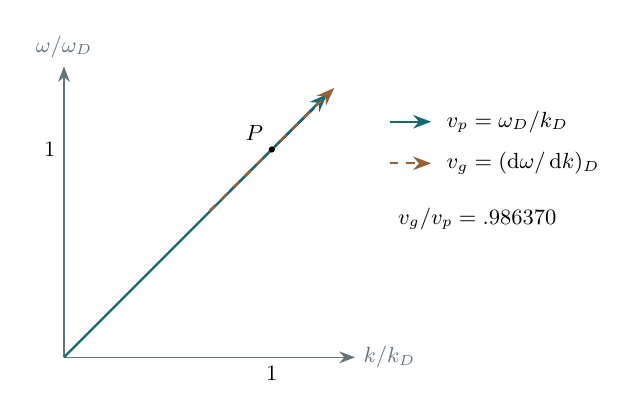
\begin{tikzpicture}[scale=.88,transform shape]
\draw[axis] (0,0)--(4.2,0) node[right] {$k/k_D$};\draw[axis] (0,0)--(0,4.2) node[above] {$\omega/\omega_D$};
\draw[thick,color=ink] plot coordinates {(2.3937945,2.4000000) (2.3988294,2.4050000) (2.4038646,2.4100000) (2.4089001,2.4150000) (2.4139358,2.4200000) (2.4189718,2.4250000) (2.4240081,2.4300000) (2.4290447,2.4350000) (2.4340815,2.4400000) (2.4391186,2.4450000) (2.4441560,2.4500000) (2.4491937,2.4550000) (2.4542316,2.4600000) (2.4592698,2.4650000) (2.4643083,2.4700000) (2.4693471,2.4750000) (2.4743861,2.4800000) (2.4794255,2.4850000) (2.4844651,2.4900000) (2.4895049,2.4950000) (2.4945451,2.5000000) (2.4995855,2.5050000) (2.5046262,2.5100000) (2.5096672,2.5150000) (2.5147085,2.5200000) (2.5197500,2.5250000) (2.5247918,2.5300000) (2.5298339,2.5350000) (2.5348763,2.5400000) (2.5399190,2.5450000) (2.5449619,2.5500000) (2.5500051,2.5550000) (2.5550486,2.5600000) (2.5600924,2.5650000) (2.5651365,2.5700000) (2.5701808,2.5750000) (2.5752255,2.5800000) (2.5802704,2.5850000) (2.5853156,2.5900000) (2.5903610,2.5950000) (2.5954068,2.6000000) (2.6004528,2.6050000) (2.6054992,2.6100000) (2.6105458,2.6150000) (2.6155927,2.6200000) (2.6206398,2.6250000) (2.6256873,2.6300000) (2.6307350,2.6350000) (2.6357831,2.6400000) (2.6408314,2.6450000) (2.6458800,2.6500000) (2.6509288,2.6550000) (2.6559780,2.6600000) (2.6610275,2.6650000) (2.6660772,2.6700000) (2.6711272,2.6750000) (2.6761775,2.6800000) (2.6812281,2.6850000) (2.6862790,2.6900000) (2.6913302,2.6950000) (2.6963816,2.7000000) (2.7014334,2.7050000) (2.7064854,2.7100000) (2.7115377,2.7150000) (2.7165903,2.7200000) (2.7216432,2.7250000) (2.7266964,2.7300000) (2.7317499,2.7350000) (2.7368036,2.7400000) (2.7418577,2.7450000) (2.7469120,2.7500000) (2.7519666,2.7550000) (2.7570215,2.7600000) (2.7620767,2.7650000) (2.7671322,2.7700000) (2.7721880,2.7750000) (2.7772441,2.7800000) (2.7823004,2.7850000) (2.7873571,2.7900000) (2.7924140,2.7950000) (2.7974713,2.8000000) (2.8025288,2.8050000) (2.8075866,2.8100000) (2.8126447,2.8150000) (2.8177031,2.8200000) (2.8227618,2.8250000) (2.8278207,2.8300000) (2.8328800,2.8350000) (2.8379396,2.8400000) (2.8429994,2.8450000) (2.8480595,2.8500000) (2.8531200,2.8550000) (2.8581807,2.8600000) (2.8632417,2.8650000) (2.8683030,2.8700000) (2.8733646,2.8750000) (2.8784265,2.8800000) (2.8834887,2.8850000) (2.8885512,2.8900000) (2.8936140,2.8950000) (2.8986770,2.9000000) (2.9037404,2.9050000) (2.9088040,2.9100000) (2.9138680,2.9150000) (2.9189322,2.9200000) (2.9239967,2.9250000) (2.9290616,2.9300000) (2.9341267,2.9350000) (2.9391921,2.9400000) (2.9442578,2.9450000) (2.9493238,2.9500000) (2.9543901,2.9550000) (2.9594567,2.9600000) (2.9645236,2.9650000) (2.9695908,2.9700000) (2.9746582,2.9750000) (2.9797260,2.9800000) (2.9847940,2.9850000) (2.9898624,2.9900000) (2.9949311,2.9950000) (3.0000000,3.0000000) (3.0050692,3.0050000) (3.0101388,3.0100000) (3.0152086,3.0150000) (3.0202787,3.0200000) (3.0253491,3.0250000) (3.0304199,3.0300000) (3.0354909,3.0350000) (3.0405622,3.0400000) (3.0456338,3.0450000) (3.0507057,3.0500000) (3.0557779,3.0550000) (3.0608504,3.0600000) (3.0659231,3.0650000) (3.0709962,3.0700000) (3.0760696,3.0750000) (3.0811433,3.0800000) (3.0862172,3.0850000) (3.0912915,3.0900000) (3.0963661,3.0950000) (3.1014409,3.1000000) (3.1065161,3.1050000) (3.1115915,3.1100000) (3.1166672,3.1150000) (3.1217433,3.1200000) (3.1268196,3.1250000) (3.1318962,3.1300000) (3.1369732,3.1350000) (3.1420504,3.1400000) (3.1471279,3.1450000) (3.1522057,3.1500000) (3.1572838,3.1550000) (3.1623622,3.1600000) (3.1674409,3.1650000) (3.1725199,3.1700000) (3.1775992,3.1750000) (3.1826788,3.1800000) (3.1877587,3.1850000) (3.1928389,3.1900000) (3.1979194,3.1950000) (3.2030001,3.2000000) (3.2080812,3.2050000) (3.2131626,3.2100000) (3.2182442,3.2150000) (3.2233262,3.2200000) (3.2284084,3.2250000) (3.2334910,3.2300000) (3.2385738,3.2350000) (3.2436570,3.2400000) (3.2487404,3.2450000) (3.2538241,3.2500000) (3.2589082,3.2550000) (3.2639925,3.2600000) (3.2690771,3.2650000) (3.2741620,3.2700000) (3.2792472,3.2750000) (3.2843327,3.2800000) (3.2894185,3.2850000) (3.2945046,3.2900000) (3.2995910,3.2950000) (3.3046777,3.3000000) (3.3097647,3.3050000) (3.3148520,3.3100000) (3.3199395,3.3150000) (3.3250274,3.3200000) (3.3301156,3.3250000) (3.3352040,3.3300000) (3.3402928,3.3350000) (3.3453818,3.3400000) (3.3504712,3.3450000) (3.3555608,3.3500000) (3.3606507,3.3550000) (3.3657410,3.3600000) (3.3708315,3.3650000) (3.3759223,3.3700000) (3.3810134,3.3750000) (3.3861048,3.3800000) (3.3911965,3.3850000) (3.3962885,3.3900000) (3.4013808,3.3950000) (3.4064733,3.4000000) (3.4115662,3.4050000) (3.4166594,3.4100000) (3.4217528,3.4150000) (3.4268466,3.4200000) (3.4319406,3.4250000) (3.4370350,3.4300000) (3.4421296,3.4350000) (3.4472245,3.4400000) (3.4523197,3.4450000) (3.4574152,3.4500000) (3.4625110,3.4550000) (3.4676071,3.4600000) (3.4727035,3.4650000) (3.4778002,3.4700000) (3.4828971,3.4750000) (3.4879944,3.4800000) (3.4930919,3.4850000) (3.4981898,3.4900000) (3.5032879,3.4950000) (3.5083863,3.5000000) (3.5134850,3.5050000) (3.5185840,3.5100000) (3.5236833,3.5150000) (3.5287829,3.5200000) (3.5338828,3.5250000) (3.5389830,3.5300000) (3.5440834,3.5350000) (3.5491841,3.5400000) (3.5542852,3.5450000) (3.5593865,3.5500000) (3.5644881,3.5550000) (3.5695900,3.5600000) (3.5746922,3.5650000) (3.5797947,3.5700000) (3.5848974,3.5750000) (3.5900005,3.5800000) (3.5951038,3.5850000) (3.6002075,3.5900000) (3.6053114,3.5950000) (3.6104156,3.6000000)};
\draw[motion] (0,0)--(3.8,3.8);
\draw[force,dashed] (2.1,2.1122671)--(3.9,3.8877329);
\fill (3,3) circle(.045);\node[above left] at (3,3) {$P$};
\node[below] at (3,0) {$1$};\node[left] at (0,3) {$1$};
\draw[motion] (4.7,3.4)--(5.3,3.4);\node[right,font=\small] at (5.4,3.4) {$v_p=\omega_D/k_D$};
\draw[force,dashed] (4.7,2.8)--(5.3,2.8);\node[right,font=\small] at (5.4,2.8) {$v_g=(\dd\omega/\dd k)_D$};
\node[right,font=\small] at (4.7,2) {$v_g/v_p=.986370$};
\end{tikzpicture}
\figcaption{解图光5.1A\quad 校准玻璃的实际局部色散，原点割线与工作点切线}
\end{minipage}\end{center}
解图光5.1C把两种速度作为波长的函数直接比较。若整条使用未校准的$A,B,C$拟合式，则工作点给$v_p=1.9793794\times10^8\,\mathrm{m/s}$、$v_g=1.9523884\times10^8\,\mathrm{m/s}$；两者相应地采用$n_{\rm fit}$及其群折射率。常数项的校准不改变$n'$，却会同量改变$n$与$n_g$，因而两种速度也随之改变。
\begin{center}\begin{minipage}{.98\linewidth}\centering
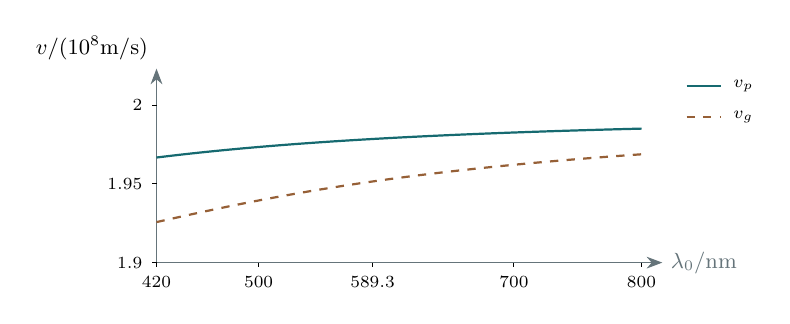
\begin{tikzpicture}[scale=.88,transform shape]
\draw[axis] (0,0)--(7.3,0) node[right] {$\lambda_0/{\rm nm}$};
\draw[axis] (0,0)--(0,2.8);
\node[above left] at (0,2.8) {$v/(10^8{\rm m/s})$};
\draw[thin] (0.000000,0)--(0.000000,-0.06);\node[below,font=\scriptsize] at (0.000000,-0.08) {$ 420 $};
\draw[thin] (1.473684,0)--(1.473684,-0.06);\node[below,font=\scriptsize] at (1.473684,-0.08) {$ 500 $};
\draw[thin] (3.118684,0)--(3.118684,-0.06);\node[below,font=\scriptsize] at (3.118684,-0.08) {$ 589.3 $};
\draw[thin] (5.157895,0)--(5.157895,-0.06);\node[below,font=\scriptsize] at (5.157895,-0.08) {$ 700 $};
\draw[thin] (7.000000,0)--(7.000000,-0.06);\node[below,font=\scriptsize] at (7.000000,-0.08) {$ 800 $};
\draw[thin] (0,0.000000)--(-.06,0.000000);\node[left,font=\scriptsize] at (-.08,0.000000) {$ 1.9 $};
\draw[thin] (0,1.136364)--(-.06,1.136364);\node[left,font=\scriptsize] at (-.08,1.136364) {$ 1.95 $};
\draw[thin] (0,2.272727)--(-.06,2.272727);\node[left,font=\scriptsize] at (-.08,2.272727) {$ 2 $};
\draw[thick,color=accent] plot coordinates {(0.0000000,1.5167512) (0.0291667,1.5203264) (0.0583333,1.5238764) (0.0875000,1.5274015) (0.1166667,1.5309018) (0.1458333,1.5343773) (0.1750000,1.5378283) (0.2041667,1.5412547) (0.2333333,1.5446567) (0.2625000,1.5480345) (0.2916667,1.5513881) (0.3208333,1.5547177) (0.3500000,1.5580235) (0.3791667,1.5613055) (0.4083333,1.5645639) (0.4375000,1.5677988) (0.4666667,1.5710104) (0.4958333,1.5741988) (0.5250000,1.5773641) (0.5541667,1.5805065) (0.5833333,1.5836262) (0.6125000,1.5867232) (0.6416667,1.5897977) (0.6708333,1.5928499) (0.7000000,1.5958799) (0.7291667,1.5988879) (0.7583333,1.6018740) (0.7875000,1.6048383) (0.8166667,1.6077810) (0.8458333,1.6107023) (0.8750000,1.6136023) (0.9041667,1.6164812) (0.9333333,1.6193391) (0.9625000,1.6221761) (0.9916667,1.6249924) (1.0208333,1.6277882) (1.0500000,1.6305636) (1.0791667,1.6333188) (1.1083333,1.6360538) (1.1375000,1.6387690) (1.1666667,1.6414643) (1.1958333,1.6441400) (1.2250000,1.6467962) (1.2541667,1.6494331) (1.2833333,1.6520508) (1.3125000,1.6546494) (1.3416667,1.6572291) (1.3708333,1.6597901) (1.4000000,1.6623325) (1.4291667,1.6648564) (1.4583333,1.6673619) (1.4875000,1.6698494) (1.5166667,1.6723187) (1.5458333,1.6747702) (1.5750000,1.6772040) (1.6041667,1.6796201) (1.6333333,1.6820188) (1.6625000,1.6844002) (1.6916667,1.6867643) (1.7208333,1.6891115) (1.7500000,1.6914417) (1.7791667,1.6937551) (1.8083333,1.6960520) (1.8375000,1.6983323) (1.8666667,1.7005962) (1.8958333,1.7028439) (1.9250000,1.7050756) (1.9541667,1.7072912) (1.9833333,1.7094910) (2.0125000,1.7116751) (2.0416667,1.7138436) (2.0708333,1.7159967) (2.1000000,1.7181344) (2.1291667,1.7202570) (2.1583333,1.7223645) (2.1875000,1.7244570) (2.2166667,1.7265347) (2.2458333,1.7285977) (2.2750000,1.7306461) (2.3041667,1.7326800) (2.3333333,1.7346996) (2.3625000,1.7367050) (2.3916667,1.7386963) (2.4208333,1.7406736) (2.4500000,1.7426370) (2.4791667,1.7445867) (2.5083333,1.7465227) (2.5375000,1.7484452) (2.5666667,1.7503543) (2.5958333,1.7522501) (2.6250000,1.7541327) (2.6541667,1.7560022) (2.6833333,1.7578587) (2.7125000,1.7597024) (2.7416667,1.7615332) (2.7708333,1.7633515) (2.8000000,1.7651572) (2.8291667,1.7669504) (2.8583333,1.7687313) (2.8875000,1.7705000) (2.9166667,1.7722565) (2.9458333,1.7740010) (2.9750000,1.7757335) (3.0041667,1.7774542) (3.0333333,1.7791632) (3.0625000,1.7808605) (3.0916667,1.7825463) (3.1208333,1.7842206) (3.1500000,1.7858836) (3.1791667,1.7875353) (3.2083333,1.7891759) (3.2375000,1.7908053) (3.2666667,1.7924238) (3.2958333,1.7940314) (3.3250000,1.7956282) (3.3541667,1.7972142) (3.3833333,1.7987897) (3.4125000,1.8003546) (3.4416667,1.8019090) (3.4708333,1.8034531) (3.5000000,1.8049869) (3.5291667,1.8065105) (3.5583333,1.8080240) (3.5875000,1.8095274) (3.6166667,1.8110209) (3.6458333,1.8125046) (3.6750000,1.8139784) (3.7041667,1.8154426) (3.7333333,1.8168971) (3.7625000,1.8183421) (3.7916667,1.8197776) (3.8208333,1.8212037) (3.8500000,1.8226205) (3.8791667,1.8240280) (3.9083333,1.8254264) (3.9375000,1.8268157) (3.9666667,1.8281960) (3.9958333,1.8295673) (4.0250000,1.8309297) (4.0541667,1.8322834) (4.0833333,1.8336283) (4.1125000,1.8349646) (4.1416667,1.8362923) (4.1708333,1.8376114) (4.2000000,1.8389221) (4.2291667,1.8402244) (4.2583333,1.8415184) (4.2875000,1.8428042) (4.3166667,1.8440817) (4.3458333,1.8453512) (4.3750000,1.8466126) (4.4041667,1.8478660) (4.4333333,1.8491115) (4.4625000,1.8503491) (4.4916667,1.8515789) (4.5208333,1.8528010) (4.5500000,1.8540154) (4.5791667,1.8552221) (4.6083333,1.8564214) (4.6375000,1.8576131) (4.6666667,1.8587974) (4.6958333,1.8599743) (4.7250000,1.8611439) (4.7541667,1.8623062) (4.7833333,1.8634614) (4.8125000,1.8646093) (4.8416667,1.8657502) (4.8708333,1.8668841) (4.9000000,1.8680109) (4.9291667,1.8691309) (4.9583333,1.8702439) (4.9875000,1.8713502) (5.0166667,1.8724496) (5.0458333,1.8735424) (5.0750000,1.8746285) (5.1041667,1.8757080) (5.1333333,1.8767809) (5.1625000,1.8778473) (5.1916667,1.8789073) (5.2208333,1.8799608) (5.2500000,1.8810080) (5.2791667,1.8820489) (5.3083333,1.8830835) (5.3375000,1.8841119) (5.3666667,1.8851341) (5.3958333,1.8861502) (5.4250000,1.8871602) (5.4541667,1.8881643) (5.4833333,1.8891623) (5.5125000,1.8901544) (5.5416667,1.8911406) (5.5708333,1.8921209) (5.6000000,1.8930955) (5.6291667,1.8940643) (5.6583333,1.8950274) (5.6875000,1.8959848) (5.7166667,1.8969366) (5.7458333,1.8978828) (5.7750000,1.8988234) (5.8041667,1.8997586) (5.8333333,1.9006883) (5.8625000,1.9016126) (5.8916667,1.9025314) (5.9208333,1.9034450) (5.9500000,1.9043533) (5.9791667,1.9052562) (6.0083333,1.9061540) (6.0375000,1.9070466) (6.0666667,1.9079341) (6.0958333,1.9088164) (6.1250000,1.9096937) (6.1541667,1.9105659) (6.1833333,1.9114332) (6.2125000,1.9122954) (6.2416667,1.9131528) (6.2708333,1.9140053) (6.3000000,1.9148529) (6.3291667,1.9156958) (6.3583333,1.9165338) (6.3875000,1.9173671) (6.4166667,1.9181957) (6.4458333,1.9190196) (6.4750000,1.9198389) (6.5041667,1.9206536) (6.5333333,1.9214637) (6.5625000,1.9222692) (6.5916667,1.9230703) (6.6208333,1.9238668) (6.6500000,1.9246590) (6.6791667,1.9254467) (6.7083333,1.9262300) (6.7375000,1.9270090) (6.7666667,1.9277837) (6.7958333,1.9285541) (6.8250000,1.9293202) (6.8541667,1.9300821) (6.8833333,1.9308399) (6.9125000,1.9315934) (6.9416667,1.9323428) (6.9708333,1.9330881) (7.0000000,1.9338294)};
\draw[thick,color=accent] (7.65,2.55)--(8.15,2.55);\node[right,font=\scriptsize] at (8.2,2.55) {$v_p$};
\draw[thick,dashed,color=warm] plot coordinates {(0.0000000,0.5849142) (0.0291667,0.5914558) (0.0583333,0.5979953) (0.0875000,0.6045315) (0.1166667,0.6110631) (0.1458333,0.6175891) (0.1750000,0.6241083) (0.2041667,0.6306198) (0.2333333,0.6371226) (0.2625000,0.6436157) (0.2916667,0.6500981) (0.3208333,0.6565690) (0.3500000,0.6630277) (0.3791667,0.6694732) (0.4083333,0.6759048) (0.4375000,0.6823218) (0.4666667,0.6887234) (0.4958333,0.6951091) (0.5250000,0.7014781) (0.5541667,0.7078299) (0.5833333,0.7141638) (0.6125000,0.7204793) (0.6416667,0.7267759) (0.6708333,0.7330531) (0.7000000,0.7393104) (0.7291667,0.7455473) (0.7583333,0.7517633) (0.7875000,0.7579582) (0.8166667,0.7641314) (0.8458333,0.7702826) (0.8750000,0.7764115) (0.9041667,0.7825176) (0.9333333,0.7886008) (0.9625000,0.7946606) (0.9916667,0.8006968) (1.0208333,0.8067092) (1.0500000,0.8126974) (1.0791667,0.8186613) (1.1083333,0.8246005) (1.1375000,0.8305150) (1.1666667,0.8364045) (1.1958333,0.8422688) (1.2250000,0.8481077) (1.2541667,0.8539211) (1.2833333,0.8597089) (1.3125000,0.8654708) (1.3416667,0.8712068) (1.3708333,0.8769168) (1.4000000,0.8826007) (1.4291667,0.8882582) (1.4583333,0.8938895) (1.4875000,0.8994944) (1.5166667,0.9050727) (1.5458333,0.9106245) (1.5750000,0.9161498) (1.6041667,0.9216484) (1.6333333,0.9271203) (1.6625000,0.9325655) (1.6916667,0.9379840) (1.7208333,0.9433757) (1.7500000,0.9487406) (1.7791667,0.9540788) (1.8083333,0.9593903) (1.8375000,0.9646749) (1.8666667,0.9699328) (1.8958333,0.9751640) (1.9250000,0.9803685) (1.9541667,0.9855463) (1.9833333,0.9906975) (2.0125000,0.9958220) (2.0416667,1.0009199) (2.0708333,1.0059914) (2.1000000,1.0110363) (2.1291667,1.0160548) (2.1583333,1.0210470) (2.1875000,1.0260128) (2.2166667,1.0309524) (2.2458333,1.0358657) (2.2750000,1.0407530) (2.3041667,1.0456142) (2.3333333,1.0504495) (2.3625000,1.0552588) (2.3916667,1.0600424) (2.4208333,1.0648002) (2.4500000,1.0695323) (2.4791667,1.0742389) (2.5083333,1.0789200) (2.5375000,1.0835757) (2.5666667,1.0882062) (2.5958333,1.0928114) (2.6250000,1.0973916) (2.6541667,1.1019467) (2.6833333,1.1064770) (2.7125000,1.1109824) (2.7416667,1.1154631) (2.7708333,1.1199193) (2.8000000,1.1243509) (2.8291667,1.1287582) (2.8583333,1.1331412) (2.8875000,1.1375000) (2.9166667,1.1418348) (2.9458333,1.1461456) (2.9750000,1.1504325) (3.0041667,1.1546958) (3.0333333,1.1589354) (3.0625000,1.1631515) (3.0916667,1.1673443) (3.1208333,1.1715137) (3.1500000,1.1756600) (3.1791667,1.1797833) (3.2083333,1.1838837) (3.2375000,1.1879612) (3.2666667,1.1920160) (3.2958333,1.1960483) (3.3250000,1.2000581) (3.3541667,1.2040456) (3.3833333,1.2080108) (3.4125000,1.2119540) (3.4416667,1.2158751) (3.4708333,1.2197744) (3.5000000,1.2236520) (3.5291667,1.2275079) (3.5583333,1.2313423) (3.5875000,1.2351553) (3.6166667,1.2389470) (3.6458333,1.2427176) (3.6750000,1.2464672) (3.7041667,1.2501958) (3.7333333,1.2539037) (3.7625000,1.2575908) (3.7916667,1.2612574) (3.8208333,1.2649036) (3.8500000,1.2685294) (3.8791667,1.2721350) (3.9083333,1.2757205) (3.9375000,1.2792861) (3.9666667,1.2828318) (3.9958333,1.2863577) (4.0250000,1.2898641) (4.0541667,1.2933509) (4.0833333,1.2968183) (4.1125000,1.3002665) (4.1416667,1.3036955) (4.1708333,1.3071054) (4.2000000,1.3104964) (4.2291667,1.3138686) (4.2583333,1.3172221) (4.2875000,1.3205570) (4.3166667,1.3238734) (4.3458333,1.3271715) (4.3750000,1.3304513) (4.4041667,1.3337129) (4.4333333,1.3369565) (4.4625000,1.3401822) (4.4916667,1.3433901) (4.5208333,1.3465802) (4.5500000,1.3497528) (4.5791667,1.3529079) (4.6083333,1.3560456) (4.6375000,1.3591660) (4.6666667,1.3622693) (4.6958333,1.3653555) (4.7250000,1.3684247) (4.7541667,1.3714772) (4.7833333,1.3745128) (4.8125000,1.3775319) (4.8416667,1.3805343) (4.8708333,1.3835204) (4.9000000,1.3864901) (4.9291667,1.3894437) (4.9583333,1.3923810) (4.9875000,1.3953024) (5.0166667,1.3982079) (5.0458333,1.4010975) (5.0750000,1.4039714) (5.1041667,1.4068297) (5.1333333,1.4096724) (5.1625000,1.4124997) (5.1916667,1.4153117) (5.2208333,1.4181085) (5.2500000,1.4208901) (5.2791667,1.4236567) (5.3083333,1.4264084) (5.3375000,1.4291452) (5.3666667,1.4318672) (5.3958333,1.4345746) (5.4250000,1.4372674) (5.4541667,1.4399457) (5.4833333,1.4426096) (5.5125000,1.4452593) (5.5416667,1.4478947) (5.5708333,1.4505160) (5.6000000,1.4531233) (5.6291667,1.4557167) (5.6583333,1.4582962) (5.6875000,1.4608620) (5.7166667,1.4634141) (5.7458333,1.4659526) (5.7750000,1.4684776) (5.8041667,1.4709892) (5.8333333,1.4734874) (5.8625000,1.4759725) (5.8916667,1.4784443) (5.9208333,1.4809031) (5.9500000,1.4833489) (5.9791667,1.4857818) (6.0083333,1.4882019) (6.0375000,1.4906092) (6.0666667,1.4930038) (6.0958333,1.4953859) (6.1250000,1.4977554) (6.1541667,1.5001126) (6.1833333,1.5024574) (6.2125000,1.5047899) (6.2416667,1.5071102) (6.2708333,1.5094184) (6.3000000,1.5117146) (6.3291667,1.5139988) (6.3583333,1.5162712) (6.3875000,1.5185317) (6.4166667,1.5207805) (6.4458333,1.5230176) (6.4750000,1.5252432) (6.5041667,1.5274572) (6.5333333,1.5296598) (6.5625000,1.5318510) (6.5916667,1.5340310) (6.6208333,1.5361997) (6.6500000,1.5383572) (6.6791667,1.5405037) (6.7083333,1.5426392) (6.7375000,1.5447637) (6.7666667,1.5468773) (6.7958333,1.5489801) (6.8250000,1.5510722) (6.8541667,1.5531536) (6.8833333,1.5552244) (6.9125000,1.5572847) (6.9416667,1.5593345) (6.9708333,1.5613739) (7.0000000,1.5634030)};
\draw[thick,dashed,color=warm] (7.65,2.0999999999999996)--(8.15,2.0999999999999996);\node[right,font=\scriptsize] at (8.2,2.0999999999999996) {$v_g$};
\end{tikzpicture}
\figcaption{解图光5.1C\quad 可见光局部模型中群速低于相速}
\end{minipage}\end{center}
弱色散的一次近似由同一分母展开得到。令$\eta=\lambda_0n'/n=-.01381846$，则
\[
v_g=\frac cn\frac1{1-\eta}
=\frac cn(1+\eta+O(\eta^2)).
\]
一次式给$v_g^{(1)}=1.9511605\times10^8\,\mathrm{m/s}$，精确群速关系给$1.9515331\times10^8\,\mathrm{m/s}$。两者相对差为
\[
 \frac{v_g-v_g^{(1)}}{v_g}
 =1-(1+\eta)(1-\eta)=\eta^2=.000190950=0.0190950\%.
\]
解图光5.1D显示这一误差随波长变化，纵轴以百分数表示$\eta^2$。
\begin{center}\begin{minipage}{.98\linewidth}\centering
\begin{tikzpicture}[scale=.88,transform shape]
\draw[axis] (0,0.0)--(7.3,0.0) node[right] {$\lambda_0/{\rm nm}$};
\draw[axis] (0,0)--(0,2.8);
\node[above left] at (0,2.8) {$\text{相对差}/\%$};
\draw[thin] (0.000000,0.0)--(0.000000,-0.06);\node[below,font=\scriptsize] at (0.000000,-0.08) {$ 420 $};
\draw[thin] (1.473684,0.0)--(1.473684,-0.06);\node[below,font=\scriptsize] at (1.473684,-0.08) {$ 500 $};
\draw[thin] (3.118684,0.0)--(3.118684,-0.06);\node[below,font=\scriptsize] at (3.118684,-0.08) {$ 589.3 $};
\draw[thin] (5.157895,0.0)--(5.157895,-0.06);\node[below,font=\scriptsize] at (5.157895,-0.08) {$ 700 $};
\draw[thin] (7.000000,0.0)--(7.000000,-0.06);\node[below,font=\scriptsize] at (7.000000,-0.08) {$ 800 $};
\draw[thin] (0,0.000000)--(-.06,0.000000);\node[left,font=\scriptsize] at (-.08,0.000000) {$ 0 $};
\draw[thin] (0,0.833333)--(-.06,0.833333);\node[left,font=\scriptsize] at (-.08,0.833333) {$ 0.02 $};
\draw[thin] (0,1.666667)--(-.06,1.666667);\node[left,font=\scriptsize] at (-.08,1.666667) {$ 0.04 $};
\draw[thin] (0,2.500000)--(-.06,2.500000);\node[left,font=\scriptsize] at (-.08,2.500000) {$ 0.06 $};
\draw[thick,color=accent] plot coordinates {(0.0000000,1.8887759) (0.0291667,1.8762083) (0.0583333,1.8635944) (0.0875000,1.8509403) (0.1166667,1.8382522) (0.1458333,1.8255359) (0.1750000,1.8127971) (0.2041667,1.8000412) (0.2333333,1.7872731) (0.2625000,1.7744979) (0.2916667,1.7617203) (0.3208333,1.7489448) (0.3500000,1.7361757) (0.3791667,1.7234171) (0.4083333,1.7106730) (0.4375000,1.6979470) (0.4666667,1.6852429) (0.4958333,1.6725639) (0.5250000,1.6599135) (0.5541667,1.6472946) (0.5833333,1.6347103) (0.6125000,1.6221633) (0.6416667,1.6096564) (0.6708333,1.5971921) (0.7000000,1.5847728) (0.7291667,1.5724009) (0.7583333,1.5600784) (0.7875000,1.5478075) (0.8166667,1.5355901) (0.8458333,1.5234280) (0.8750000,1.5113231) (0.9041667,1.4992770) (0.9333333,1.4872912) (0.9625000,1.4753671) (0.9916667,1.4635063) (1.0208333,1.4517099) (1.0500000,1.4399792) (1.0791667,1.4283153) (1.1083333,1.4167192) (1.1375000,1.4051920) (1.1666667,1.3937347) (1.1958333,1.3823479) (1.2250000,1.3710326) (1.2541667,1.3597894) (1.2833333,1.3486191) (1.3125000,1.3375222) (1.3416667,1.3264993) (1.3708333,1.3155509) (1.4000000,1.3046775) (1.4291667,1.2938795) (1.4583333,1.2831572) (1.4875000,1.2725110) (1.5166667,1.2619412) (1.5458333,1.2514479) (1.5750000,1.2410314) (1.6041667,1.2306919) (1.6333333,1.2204295) (1.6625000,1.2102443) (1.6916667,1.2001363) (1.7208333,1.1901055) (1.7500000,1.1801521) (1.7791667,1.1702759) (1.8083333,1.1604769) (1.8375000,1.1507550) (1.8666667,1.1411102) (1.8958333,1.1315422) (1.9250000,1.1220510) (1.9541667,1.1126363) (1.9833333,1.1032980) (2.0125000,1.0940359) (2.0416667,1.0848498) (2.0708333,1.0757393) (2.1000000,1.0667043) (2.1291667,1.0577444) (2.1583333,1.0488594) (2.1875000,1.0400489) (2.2166667,1.0313127) (2.2458333,1.0226504) (2.2750000,1.0140616) (2.3041667,1.0055461) (2.3333333,0.9971034) (2.3625000,0.9887331) (2.3916667,0.9804349) (2.4208333,0.9722084) (2.4500000,0.9640532) (2.4791667,0.9559688) (2.5083333,0.9479548) (2.5375000,0.9400109) (2.5666667,0.9321366) (2.5958333,0.9243314) (2.6250000,0.9165949) (2.6541667,0.9089266) (2.6833333,0.9013262) (2.7125000,0.8937931) (2.7416667,0.8863269) (2.7708333,0.8789270) (2.8000000,0.8715932) (2.8291667,0.8643248) (2.8583333,0.8571214) (2.8875000,0.8499825) (2.9166667,0.8429077) (2.9458333,0.8358964) (2.9750000,0.8289483) (3.0041667,0.8220627) (3.0333333,0.8152392) (3.0625000,0.8084774) (3.0916667,0.8017767) (3.1208333,0.7951367) (3.1500000,0.7885568) (3.1791667,0.7820367) (3.2083333,0.7755757) (3.2375000,0.7691735) (3.2666667,0.7628295) (3.2958333,0.7565432) (3.3250000,0.7503142) (3.3541667,0.7441420) (3.3833333,0.7380261) (3.4125000,0.7319660) (3.4416667,0.7259612) (3.4708333,0.7200113) (3.5000000,0.7141158) (3.5291667,0.7082742) (3.5583333,0.7024861) (3.5875000,0.6967509) (3.6166667,0.6910683) (3.6458333,0.6854376) (3.6750000,0.6798586) (3.7041667,0.6743307) (3.7333333,0.6688534) (3.7625000,0.6634263) (3.7916667,0.6580490) (3.8208333,0.6527210) (3.8500000,0.6474418) (3.8791667,0.6422110) (3.9083333,0.6370282) (3.9375000,0.6318929) (3.9666667,0.6268046) (3.9958333,0.6217630) (4.0250000,0.6167676) (4.0541667,0.6118180) (4.0833333,0.6069138) (4.1125000,0.6020544) (4.1416667,0.5972396) (4.1708333,0.5924688) (4.2000000,0.5877418) (4.2291667,0.5830580) (4.2583333,0.5784170) (4.2875000,0.5738185) (4.3166667,0.5692620) (4.3458333,0.5647472) (4.3750000,0.5602736) (4.4041667,0.5558409) (4.4333333,0.5514487) (4.4625000,0.5470965) (4.4916667,0.5427840) (4.5208333,0.5385109) (4.5500000,0.5342766) (4.5791667,0.5300810) (4.6083333,0.5259235) (4.6375000,0.5218038) (4.6666667,0.5177216) (4.6958333,0.5136765) (4.7250000,0.5096682) (4.7541667,0.5056962) (4.7833333,0.5017602) (4.8125000,0.4978599) (4.8416667,0.4939950) (4.8708333,0.4901650) (4.9000000,0.4863697) (4.9291667,0.4826087) (4.9583333,0.4788817) (4.9875000,0.4751883) (5.0166667,0.4715283) (5.0458333,0.4679012) (5.0750000,0.4643068) (5.1041667,0.4607448) (5.1333333,0.4572148) (5.1625000,0.4537165) (5.1916667,0.4502497) (5.2208333,0.4468139) (5.2500000,0.4434090) (5.2791667,0.4400345) (5.3083333,0.4366903) (5.3375000,0.4333760) (5.3666667,0.4300912) (5.3958333,0.4268358) (5.4250000,0.4236095) (5.4541667,0.4204119) (5.4833333,0.4172428) (5.5125000,0.4141018) (5.5416667,0.4109888) (5.5708333,0.4079034) (5.6000000,0.4048454) (5.6291667,0.4018145) (5.6583333,0.3988104) (5.6875000,0.3958330) (5.7166667,0.3928818) (5.7458333,0.3899567) (5.7750000,0.3870574) (5.8041667,0.3841836) (5.8333333,0.3813352) (5.8625000,0.3785118) (5.8916667,0.3757132) (5.9208333,0.3729391) (5.9500000,0.3701894) (5.9791667,0.3674638) (6.0083333,0.3647620) (6.0375000,0.3620839) (6.0666667,0.3594291) (6.0958333,0.3567975) (6.1250000,0.3541889) (6.1541667,0.3516029) (6.1833333,0.3490394) (6.2125000,0.3464982) (6.2416667,0.3439791) (6.2708333,0.3414818) (6.3000000,0.3390061) (6.3291667,0.3365519) (6.3583333,0.3341188) (6.3875000,0.3317067) (6.4166667,0.3293155) (6.4458333,0.3269448) (6.4750000,0.3245945) (6.5041667,0.3222645) (6.5333333,0.3199544) (6.5625000,0.3176641) (6.5916667,0.3153935) (6.6208333,0.3131423) (6.6500000,0.3109103) (6.6791667,0.3086973) (6.7083333,0.3065033) (6.7375000,0.3043279) (6.7666667,0.3021710) (6.7958333,0.3000325) (6.8250000,0.2979121) (6.8541667,0.2958097) (6.8833333,0.2937251) (6.9125000,0.2916581) (6.9416667,0.2896086) (6.9708333,0.2875763) (7.0000000,0.2855612)};
\end{tikzpicture}
\figcaption{解图光5.1D\quad 弱色散一次式低于完整分母结果，相对差等于$\eta^2$}
\end{minipage}\end{center}
介质内波长形式的Rayleigh关系也可由链式求导得到。由$\lambda_m=\lambda_0/n$，
\[
 \frac{\dd\lambda_m}{\dd\lambda_0}=\frac{n_g}{n^2},\qquad
 \frac{\dd v_p}{\dd\lambda_m}=-\frac{c n'}{n_g},\qquad
 v_p-\lambda_m\frac{\dd v_p}{\dd\lambda_m}=\frac c{n_g}.
\]
这个严格表达中的自变量是$\lambda_m$；以真空波长$\lambda_0$展开时则回到前面的群折射率分母。群速描述中心频率附近的一次相位差传播，透明窄带条件下也对应能量包络的传播。带宽扩大后，$k''=\dd^2k/\dd\omega^2$产生频率相关的群延迟，包络还会展宽，传播时需同时保留这一二阶项。


\Needspace{8\baselineskip}

\pdfbookmark[3]{关键洞察}{q1-h5}

\subsection*{关键洞察}

相速和群速的差由频率邻域的斜率决定。折射率是否大于1只确定相速相对真空的大小；群速与相速的先后还取决于$n'$。常数项平移不改变斜率，却影响速度分母，局部测量校准因而有具体的代数意义。

\Needspace{8\baselineskip}

\pdfbookmark[3]{易错点}{q1-h6}

\subsection*{易错点}

\begin{itemize}
\item Rayleigh式中的波长为介质内$\lambda_m$；真空波长使用$n_g=n-\lambda_0n'$并保留分母。
\item 用$n'$的正负比较两速度：本题$n'<0$使$n_g>n$，群速较小。
\item nm波长与每nm导数成对使用；把波长改为m时导数也按每m转换。
\item 完整分母和一次展开分别报告，$\eta^2$给出本题一次式的误差尺度。
\end{itemize}

\Needspace{8\baselineskip}

\pdfbookmark[3]{课堂讲解建议}{q1-h7}

\subsection*{课堂讲解建议}

先在A图指出原点割线与切线，再从波包的两频率相位差解释切线斜率。计算导数以后只改变常数项，询问$n'$、$n$、$n_g$各怎样变化，让学生用一行代数说明校准方案。最后算$\eta^2$并在D图定位工作波长，将所报速度位数与近似误差对应。二阶色散变式再用群延迟差连接脉冲展宽。

\Needspace{8\baselineskip}

\pdfbookmark[3]{变式训练}{q1-h8}

\subsection*{变式训练}

\begin{enumerate}
\item \textbf{折射率与频率无关。}取$n_0=1.5$，求相速、群速及一米传播时间。

变图光5.1V1的色散线为$\omega=(c/n_0)k$，通过原点，任意点的割线和切线重合。因此$v_p=v_g=c/n_0=2.00\times10^8\,\mathrm{m/s}$。窄带包络通过一米需$L/v_g=5.00\,\mathrm{ns}$，所有频率的群延迟相同，二阶导数$k''=0$，该模型下包络只作平移。
\begin{center}\begin{minipage}{.98\linewidth}\centering
\begin{tikzpicture}[scale=.88,transform shape]
\draw[axis] (0,0.0)--(7.3,0.0) node[right] {$k/k_*$};
\draw[axis] (0,0)--(0,2.8);
\node[above left] at (0,2.8) {$\omega/\omega_*$};
\draw[thin] (0.000000,0.0)--(0.000000,-0.06);\node[below,font=\scriptsize] at (0.000000,-0.08) {$ 0 $};
\draw[thin] (2.692308,0.0)--(2.692308,-0.06);\node[below,font=\scriptsize] at (2.692308,-0.08) {$ 0.5 $};
\draw[thin] (5.384615,0.0)--(5.384615,-0.06);\node[below,font=\scriptsize] at (5.384615,-0.08) {$ 1 $};
\draw[thin] (7.000000,0.0)--(7.000000,-0.06);\node[below,font=\scriptsize] at (7.000000,-0.08) {$ 1.3 $};
\draw[thin] (0,0.000000)--(-.06,0.000000);\node[left,font=\scriptsize] at (-.08,0.000000) {$ 0 $};
\draw[thin] (0,0.925926)--(-.06,0.925926);\node[left,font=\scriptsize] at (-.08,0.925926) {$ 0.5 $};
\draw[thin] (0,1.851852)--(-.06,1.851852);\node[left,font=\scriptsize] at (-.08,1.851852) {$ 1 $};
\draw[thick,color=accent] plot coordinates {(0.0000000,0.0000000) (0.0291667,0.0100309) (0.0583333,0.0200617) (0.0875000,0.0300926) (0.1166667,0.0401235) (0.1458333,0.0501543) (0.1750000,0.0601852) (0.2041667,0.0702160) (0.2333333,0.0802469) (0.2625000,0.0902778) (0.2916667,0.1003086) (0.3208333,0.1103395) (0.3500000,0.1203704) (0.3791667,0.1304012) (0.4083333,0.1404321) (0.4375000,0.1504630) (0.4666667,0.1604938) (0.4958333,0.1705247) (0.5250000,0.1805556) (0.5541667,0.1905864) (0.5833333,0.2006173) (0.6125000,0.2106481) (0.6416667,0.2206790) (0.6708333,0.2307099) (0.7000000,0.2407407) (0.7291667,0.2507716) (0.7583333,0.2608025) (0.7875000,0.2708333) (0.8166667,0.2808642) (0.8458333,0.2908951) (0.8750000,0.3009259) (0.9041667,0.3109568) (0.9333333,0.3209877) (0.9625000,0.3310185) (0.9916667,0.3410494) (1.0208333,0.3510802) (1.0500000,0.3611111) (1.0791667,0.3711420) (1.1083333,0.3811728) (1.1375000,0.3912037) (1.1666667,0.4012346) (1.1958333,0.4112654) (1.2250000,0.4212963) (1.2541667,0.4313272) (1.2833333,0.4413580) (1.3125000,0.4513889) (1.3416667,0.4614198) (1.3708333,0.4714506) (1.4000000,0.4814815) (1.4291667,0.4915123) (1.4583333,0.5015432) (1.4875000,0.5115741) (1.5166667,0.5216049) (1.5458333,0.5316358) (1.5750000,0.5416667) (1.6041667,0.5516975) (1.6333333,0.5617284) (1.6625000,0.5717593) (1.6916667,0.5817901) (1.7208333,0.5918210) (1.7500000,0.6018519) (1.7791667,0.6118827) (1.8083333,0.6219136) (1.8375000,0.6319444) (1.8666667,0.6419753) (1.8958333,0.6520062) (1.9250000,0.6620370) (1.9541667,0.6720679) (1.9833333,0.6820988) (2.0125000,0.6921296) (2.0416667,0.7021605) (2.0708333,0.7121914) (2.1000000,0.7222222) (2.1291667,0.7322531) (2.1583333,0.7422840) (2.1875000,0.7523148) (2.2166667,0.7623457) (2.2458333,0.7723765) (2.2750000,0.7824074) (2.3041667,0.7924383) (2.3333333,0.8024691) (2.3625000,0.8125000) (2.3916667,0.8225309) (2.4208333,0.8325617) (2.4500000,0.8425926) (2.4791667,0.8526235) (2.5083333,0.8626543) (2.5375000,0.8726852) (2.5666667,0.8827160) (2.5958333,0.8927469) (2.6250000,0.9027778) (2.6541667,0.9128086) (2.6833333,0.9228395) (2.7125000,0.9328704) (2.7416667,0.9429012) (2.7708333,0.9529321) (2.8000000,0.9629630) (2.8291667,0.9729938) (2.8583333,0.9830247) (2.8875000,0.9930556) (2.9166667,1.0030864) (2.9458333,1.0131173) (2.9750000,1.0231481) (3.0041667,1.0331790) (3.0333333,1.0432099) (3.0625000,1.0532407) (3.0916667,1.0632716) (3.1208333,1.0733025) (3.1500000,1.0833333) (3.1791667,1.0933642) (3.2083333,1.1033951) (3.2375000,1.1134259) (3.2666667,1.1234568) (3.2958333,1.1334877) (3.3250000,1.1435185) (3.3541667,1.1535494) (3.3833333,1.1635802) (3.4125000,1.1736111) (3.4416667,1.1836420) (3.4708333,1.1936728) (3.5000000,1.2037037) (3.5291667,1.2137346) (3.5583333,1.2237654) (3.5875000,1.2337963) (3.6166667,1.2438272) (3.6458333,1.2538580) (3.6750000,1.2638889) (3.7041667,1.2739198) (3.7333333,1.2839506) (3.7625000,1.2939815) (3.7916667,1.3040123) (3.8208333,1.3140432) (3.8500000,1.3240741) (3.8791667,1.3341049) (3.9083333,1.3441358) (3.9375000,1.3541667) (3.9666667,1.3641975) (3.9958333,1.3742284) (4.0250000,1.3842593) (4.0541667,1.3942901) (4.0833333,1.4043210) (4.1125000,1.4143519) (4.1416667,1.4243827) (4.1708333,1.4344136) (4.2000000,1.4444444) (4.2291667,1.4544753) (4.2583333,1.4645062) (4.2875000,1.4745370) (4.3166667,1.4845679) (4.3458333,1.4945988) (4.3750000,1.5046296) (4.4041667,1.5146605) (4.4333333,1.5246914) (4.4625000,1.5347222) (4.4916667,1.5447531) (4.5208333,1.5547840) (4.5500000,1.5648148) (4.5791667,1.5748457) (4.6083333,1.5848765) (4.6375000,1.5949074) (4.6666667,1.6049383) (4.6958333,1.6149691) (4.7250000,1.6250000) (4.7541667,1.6350309) (4.7833333,1.6450617) (4.8125000,1.6550926) (4.8416667,1.6651235) (4.8708333,1.6751543) (4.9000000,1.6851852) (4.9291667,1.6952160) (4.9583333,1.7052469) (4.9875000,1.7152778) (5.0166667,1.7253086) (5.0458333,1.7353395) (5.0750000,1.7453704) (5.1041667,1.7554012) (5.1333333,1.7654321) (5.1625000,1.7754630) (5.1916667,1.7854938) (5.2208333,1.7955247) (5.2500000,1.8055556) (5.2791667,1.8155864) (5.3083333,1.8256173) (5.3375000,1.8356481) (5.3666667,1.8456790) (5.3958333,1.8557099) (5.4250000,1.8657407) (5.4541667,1.8757716) (5.4833333,1.8858025) (5.5125000,1.8958333) (5.5416667,1.9058642) (5.5708333,1.9158951) (5.6000000,1.9259259) (5.6291667,1.9359568) (5.6583333,1.9459877) (5.6875000,1.9560185) (5.7166667,1.9660494) (5.7458333,1.9760802) (5.7750000,1.9861111) (5.8041667,1.9961420) (5.8333333,2.0061728) (5.8625000,2.0162037) (5.8916667,2.0262346) (5.9208333,2.0362654) (5.9500000,2.0462963) (5.9791667,2.0563272) (6.0083333,2.0663580) (6.0375000,2.0763889) (6.0666667,2.0864198) (6.0958333,2.0964506) (6.1250000,2.1064815) (6.1541667,2.1165123) (6.1833333,2.1265432) (6.2125000,2.1365741) (6.2416667,2.1466049) (6.2708333,2.1566358) (6.3000000,2.1666667) (6.3291667,2.1766975) (6.3583333,2.1867284) (6.3875000,2.1967593) (6.4166667,2.2067901) (6.4458333,2.2168210) (6.4750000,2.2268519) (6.5041667,2.2368827) (6.5333333,2.2469136) (6.5625000,2.2569444) (6.5916667,2.2669753) (6.6208333,2.2770062) (6.6500000,2.2870370) (6.6791667,2.2970679) (6.7083333,2.3070988) (6.7375000,2.3171296) (6.7666667,2.3271605) (6.7958333,2.3371914) (6.8250000,2.3472222) (6.8541667,2.3572531) (6.8833333,2.3672840) (6.9125000,2.3773148) (6.9416667,2.3873457) (6.9708333,2.3973765) (7.0000000,2.4074074)};
\end{tikzpicture}
\figcaption{变图光5.1V1\quad 常折射率使归一化色散线通过原点且斜率不变}
\end{minipage}\end{center}
\item \textbf{仅保留两项柯西式。}取$n=A+B/\lambda_0^2$，$A=1.504,B=4437\,\mathrm{nm^2}$。求$n_g$及两速度差，在589.3nm处给数值。

由$n'=-2B/\lambda_0^3$，得$n_g=A+3B/\lambda_0^2$，因此
\[
 v_p-v_g=\frac{c(n_g-n)}{nn_g}=\frac{2cB}{\lambda_0^2nn_g}>0.
\]
变图光5.1V2画出两速度随波长变化。在589.3nm处$n=1.51677664$、$n_g=1.54232991$，$v_p=1.9778786\times10^8\,\mathrm{m/s}$、$v_g=1.9451091\times10^8\,\mathrm{m/s}$。$B>0$给正常色散的正速度差。
\begin{center}\begin{minipage}{.98\linewidth}\centering
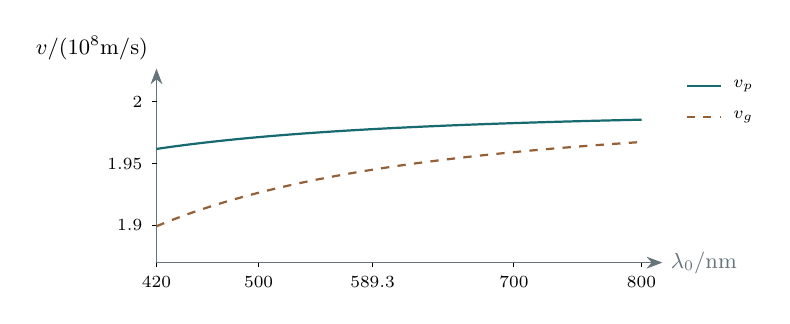
\begin{tikzpicture}[scale=.88,transform shape]
\draw[axis] (0,0)--(7.3,0) node[right] {$\lambda_0/{\rm nm}$};
\draw[axis] (0,0)--(0,2.8);
\node[above left] at (0,2.8) {$v/(10^8{\rm m/s})$};
\draw[thin] (0.000000,0)--(0.000000,-0.06);\node[below,font=\scriptsize] at (0.000000,-0.08) {$ 420 $};
\draw[thin] (1.473684,0)--(1.473684,-0.06);\node[below,font=\scriptsize] at (1.473684,-0.08) {$ 500 $};
\draw[thin] (3.118684,0)--(3.118684,-0.06);\node[below,font=\scriptsize] at (3.118684,-0.08) {$ 589.3 $};
\draw[thin] (5.157895,0)--(5.157895,-0.06);\node[below,font=\scriptsize] at (5.157895,-0.08) {$ 700 $};
\draw[thin] (7.000000,0)--(7.000000,-0.06);\node[below,font=\scriptsize] at (7.000000,-0.08) {$ 800 $};
\draw[thin] (0,0.535714)--(-.06,0.535714);\node[left,font=\scriptsize] at (-.08,0.535714) {$ 1.9 $};
\draw[thin] (0,1.428571)--(-.06,1.428571);\node[left,font=\scriptsize] at (-.08,1.428571) {$ 1.95 $};
\draw[thin] (0,2.321429)--(-.06,2.321429);\node[left,font=\scriptsize] at (-.08,2.321429) {$ 2 $};
\draw[thick,color=accent] plot coordinates {(0.0000000,1.6405414) (0.0291667,1.6448623) (0.0583333,1.6491359) (0.0875000,1.6533628) (0.1166667,1.6575437) (0.1458333,1.6616792) (0.1750000,1.6657701) (0.2041667,1.6698169) (0.2333333,1.6738203) (0.2625000,1.6777809) (0.2916667,1.6816992) (0.3208333,1.6855760) (0.3500000,1.6894117) (0.3791667,1.6932070) (0.4083333,1.6969623) (0.4375000,1.7006784) (0.4666667,1.7043556) (0.4958333,1.7079946) (0.5250000,1.7115959) (0.5541667,1.7151600) (0.5833333,1.7186873) (0.6125000,1.7221785) (0.6416667,1.7256339) (0.6708333,1.7290541) (0.7000000,1.7324396) (0.7291667,1.7357907) (0.7583333,1.7391081) (0.7875000,1.7423920) (0.8166667,1.7456431) (0.8458333,1.7488616) (0.8750000,1.7520481) (0.9041667,1.7552029) (0.9333333,1.7583265) (0.9625000,1.7614193) (0.9916667,1.7644816) (1.0208333,1.7675140) (1.0500000,1.7705167) (1.0791667,1.7734902) (1.1083333,1.7764348) (1.1375000,1.7793509) (1.1666667,1.7822388) (1.1958333,1.7850990) (1.2250000,1.7879318) (1.2541667,1.7907375) (1.2833333,1.7935164) (1.3125000,1.7962690) (1.3416667,1.7989955) (1.3708333,1.8016963) (1.4000000,1.8043716) (1.4291667,1.8070219) (1.4583333,1.8096473) (1.4875000,1.8122483) (1.5166667,1.8148251) (1.5458333,1.8173781) (1.5750000,1.8199074) (1.6041667,1.8224135) (1.6333333,1.8248965) (1.6625000,1.8273568) (1.6916667,1.8297946) (1.7208333,1.8322103) (1.7500000,1.8346040) (1.7791667,1.8369761) (1.8083333,1.8393268) (1.8375000,1.8416563) (1.8666667,1.8439650) (1.8958333,1.8462530) (1.9250000,1.8485206) (1.9541667,1.8507681) (1.9833333,1.8529956) (2.0125000,1.8552035) (2.0416667,1.8573919) (2.0708333,1.8595611) (2.1000000,1.8617113) (2.1291667,1.8638426) (2.1583333,1.8659555) (2.1875000,1.8680500) (2.2166667,1.8701263) (2.2458333,1.8721847) (2.2750000,1.8742254) (2.3041667,1.8762485) (2.3333333,1.8782544) (2.3625000,1.8802431) (2.3916667,1.8822148) (2.4208333,1.8841699) (2.4500000,1.8861083) (2.4791667,1.8880304) (2.5083333,1.8899364) (2.5375000,1.8918263) (2.5666667,1.8937003) (2.5958333,1.8955588) (2.6250000,1.8974017) (2.6541667,1.8992294) (2.6833333,1.9010419) (2.7125000,1.9028394) (2.7416667,1.9046222) (2.7708333,1.9063902) (2.8000000,1.9081438) (2.8291667,1.9098831) (2.8583333,1.9116082) (2.8875000,1.9133193) (2.9166667,1.9150165) (2.9458333,1.9166999) (2.9750000,1.9183698) (3.0041667,1.9200263) (3.0333333,1.9216695) (3.0625000,1.9232995) (3.0916667,1.9249166) (3.1208333,1.9265207) (3.1500000,1.9281122) (3.1791667,1.9296910) (3.2083333,1.9312574) (3.2375000,1.9328114) (3.2666667,1.9343533) (3.2958333,1.9358830) (3.3250000,1.9374008) (3.3541667,1.9389068) (3.3833333,1.9404011) (3.4125000,1.9418837) (3.4416667,1.9433549) (3.4708333,1.9448148) (3.5000000,1.9462634) (3.5291667,1.9477009) (3.5583333,1.9491274) (3.5875000,1.9505430) (3.6166667,1.9519479) (3.6458333,1.9533420) (3.6750000,1.9547256) (3.7041667,1.9560987) (3.7333333,1.9574615) (3.7625000,1.9588140) (3.7916667,1.9601563) (3.8208333,1.9614887) (3.8500000,1.9628110) (3.8791667,1.9641235) (3.9083333,1.9654263) (3.9375000,1.9667194) (3.9666667,1.9680029) (3.9958333,1.9692770) (4.0250000,1.9705417) (4.0541667,1.9717971) (4.0833333,1.9730433) (4.1125000,1.9742804) (4.1416667,1.9755085) (4.1708333,1.9767277) (4.2000000,1.9779380) (4.2291667,1.9791396) (4.2583333,1.9803325) (4.2875000,1.9815168) (4.3166667,1.9826926) (4.3458333,1.9838600) (4.3750000,1.9850190) (4.4041667,1.9861697) (4.4333333,1.9873123) (4.4625000,1.9884468) (4.4916667,1.9895732) (4.5208333,1.9906916) (4.5500000,1.9918022) (4.5791667,1.9929050) (4.6083333,1.9940000) (4.6375000,1.9950873) (4.6666667,1.9961671) (4.6958333,1.9972393) (4.7250000,1.9983041) (4.7541667,1.9993615) (4.7833333,2.0004116) (4.8125000,2.0014544) (4.8416667,2.0024900) (4.8708333,2.0035185) (4.9000000,2.0045400) (4.9291667,2.0055545) (4.9583333,2.0065620) (4.9875000,2.0075627) (5.0166667,2.0085566) (5.0458333,2.0095437) (5.0750000,2.0105242) (5.1041667,2.0114980) (5.1333333,2.0124653) (5.1625000,2.0134261) (5.1916667,2.0143804) (5.2208333,2.0153283) (5.2500000,2.0162700) (5.2791667,2.0172053) (5.3083333,2.0181344) (5.3375000,2.0190574) (5.3666667,2.0199743) (5.3958333,2.0208851) (5.4250000,2.0217899) (5.4541667,2.0226887) (5.4833333,2.0235817) (5.5125000,2.0244688) (5.5416667,2.0253501) (5.5708333,2.0262256) (5.6000000,2.0270955) (5.6291667,2.0279597) (5.6583333,2.0288184) (5.6875000,2.0296714) (5.7166667,2.0305190) (5.7458333,2.0313611) (5.7750000,2.0321979) (5.8041667,2.0330292) (5.8333333,2.0338552) (5.8625000,2.0346760) (5.8916667,2.0354915) (5.9208333,2.0363019) (5.9500000,2.0371071) (5.9791667,2.0379072) (6.0083333,2.0387023) (6.0375000,2.0394924) (6.0666667,2.0402775) (6.0958333,2.0410576) (6.1250000,2.0418329) (6.1541667,2.0426034) (6.1833333,2.0433690) (6.2125000,2.0441299) (6.2416667,2.0448860) (6.2708333,2.0456375) (6.3000000,2.0463843) (6.3291667,2.0471265) (6.3583333,2.0478641) (6.3875000,2.0485972) (6.4166667,2.0493258) (6.4458333,2.0500499) (6.4750000,2.0507696) (6.5041667,2.0514849) (6.5333333,2.0521959) (6.5625000,2.0529025) (6.5916667,2.0536049) (6.6208333,2.0543030) (6.6500000,2.0549969) (6.6791667,2.0556867) (6.7083333,2.0563722) (6.7375000,2.0570537) (6.7666667,2.0577311) (6.7958333,2.0584044) (6.8250000,2.0590737) (6.8541667,2.0597391) (6.8833333,2.0604004) (6.9125000,2.0610579) (6.9416667,2.0617115) (6.9708333,2.0623612) (7.0000000,2.0630070)};
\draw[thick,color=accent] (7.65,2.55)--(8.15,2.55);\node[right,font=\scriptsize] at (8.2,2.55) {$v_p$};
\draw[thick,dashed,color=warm] plot coordinates {(0.0000000,0.5247199) (0.0291667,0.5368730) (0.0583333,0.5488985) (0.0875000,0.5607981) (0.1166667,0.5725737) (0.1458333,0.5842268) (0.1750000,0.5957591) (0.2041667,0.6071723) (0.2333333,0.6184679) (0.2625000,0.6296476) (0.2916667,0.6407129) (0.3208333,0.6516654) (0.3500000,0.6625065) (0.3791667,0.6732377) (0.4083333,0.6838605) (0.4375000,0.6943764) (0.4666667,0.7047866) (0.4958333,0.7150927) (0.5250000,0.7252959) (0.5541667,0.7353977) (0.5833333,0.7453993) (0.6125000,0.7553020) (0.6416667,0.7651072) (0.6708333,0.7748160) (0.7000000,0.7844298) (0.7291667,0.7939497) (0.7583333,0.8033769) (0.7875000,0.8127126) (0.8166667,0.8219581) (0.8458333,0.8311143) (0.8750000,0.8401825) (0.9041667,0.8491638) (0.9333333,0.8580592) (0.9625000,0.8668699) (0.9916667,0.8755968) (1.0208333,0.8842411) (1.0500000,0.8928038) (1.0791667,0.9012858) (1.1083333,0.9096882) (1.1375000,0.9180119) (1.1666667,0.9262579) (1.1958333,0.9344272) (1.2250000,0.9425207) (1.2541667,0.9505394) (1.2833333,0.9584840) (1.3125000,0.9663556) (1.3416667,0.9741550) (1.3708333,0.9818831) (1.4000000,0.9895407) (1.4291667,0.9971287) (1.4583333,1.0046479) (1.4875000,1.0120992) (1.5166667,1.0194833) (1.5458333,1.0268010) (1.5750000,1.0340531) (1.6041667,1.0412404) (1.6333333,1.0483637) (1.6625000,1.0554236) (1.6916667,1.0624210) (1.7208333,1.0693566) (1.7500000,1.0762310) (1.7791667,1.0830450) (1.8083333,1.0897994) (1.8375000,1.0964947) (1.8666667,1.1031316) (1.8958333,1.1097109) (1.9250000,1.1162332) (1.9541667,1.1226991) (1.9833333,1.1291092) (2.0125000,1.1354643) (2.0416667,1.1417649) (2.0708333,1.1480116) (2.1000000,1.1542051) (2.1291667,1.1603460) (2.1583333,1.1664347) (2.1875000,1.1724720) (2.2166667,1.1784584) (2.2458333,1.1843944) (2.2750000,1.1902806) (2.3041667,1.1961176) (2.3333333,1.2019059) (2.3625000,1.2076460) (2.3916667,1.2133385) (2.4208333,1.2189839) (2.4500000,1.2245826) (2.4791667,1.2301353) (2.5083333,1.2356424) (2.5375000,1.2411043) (2.5666667,1.2465217) (2.5958333,1.2518949) (2.6250000,1.2572245) (2.6541667,1.2625108) (2.6833333,1.2677544) (2.7125000,1.2729558) (2.7416667,1.2781153) (2.7708333,1.2832334) (2.8000000,1.2883106) (2.8291667,1.2933472) (2.8583333,1.2983438) (2.8875000,1.3033007) (2.9166667,1.3082183) (2.9458333,1.3130971) (2.9750000,1.3179374) (3.0041667,1.3227397) (3.0333333,1.3275044) (3.0625000,1.3322318) (3.0916667,1.3369223) (3.1208333,1.3415763) (3.1500000,1.3461942) (3.1791667,1.3507763) (3.2083333,1.3553230) (3.2375000,1.3598348) (3.2666667,1.3643118) (3.2958333,1.3687545) (3.3250000,1.3731633) (3.3541667,1.3775384) (3.3833333,1.3818803) (3.4125000,1.3861891) (3.4416667,1.3904654) (3.4708333,1.3947093) (3.5000000,1.3989213) (3.5291667,1.4031016) (3.5583333,1.4072505) (3.5875000,1.4113684) (3.6166667,1.4154556) (3.6458333,1.4195124) (3.6750000,1.4235390) (3.7041667,1.4275358) (3.7333333,1.4315030) (3.7625000,1.4354410) (3.7916667,1.4393500) (3.8208333,1.4432304) (3.8500000,1.4470823) (3.8791667,1.4509061) (3.9083333,1.4547020) (3.9375000,1.4584703) (3.9666667,1.4622113) (3.9958333,1.4659252) (4.0250000,1.4696123) (4.0541667,1.4732728) (4.0833333,1.4769071) (4.1125000,1.4805153) (4.1416667,1.4840976) (4.1708333,1.4876545) (4.2000000,1.4911860) (4.2291667,1.4946924) (4.2583333,1.4981739) (4.2875000,1.5016309) (4.3166667,1.5050634) (4.3458333,1.5084718) (4.3750000,1.5118563) (4.4041667,1.5152170) (4.4333333,1.5185543) (4.4625000,1.5218683) (4.4916667,1.5251592) (4.5208333,1.5284272) (4.5500000,1.5316727) (4.5791667,1.5348957) (4.6083333,1.5380964) (4.6375000,1.5412752) (4.6666667,1.5444321) (4.6958333,1.5475674) (4.7250000,1.5506812) (4.7541667,1.5537738) (4.7833333,1.5568454) (4.8125000,1.5598961) (4.8416667,1.5629262) (4.8708333,1.5659357) (4.9000000,1.5689250) (4.9291667,1.5718941) (4.9583333,1.5748433) (4.9875000,1.5777727) (5.0166667,1.5806826) (5.0458333,1.5835730) (5.0750000,1.5864442) (5.1041667,1.5892963) (5.1333333,1.5921295) (5.1625000,1.5949439) (5.1916667,1.5977398) (5.2208333,1.6005172) (5.2500000,1.6032764) (5.2791667,1.6060175) (5.3083333,1.6087407) (5.3375000,1.6114461) (5.3666667,1.6141338) (5.3958333,1.6168041) (5.4250000,1.6194570) (5.4541667,1.6220928) (5.4833333,1.6247115) (5.5125000,1.6273134) (5.5416667,1.6298985) (5.5708333,1.6324670) (5.6000000,1.6350190) (5.6291667,1.6375547) (5.6583333,1.6400742) (5.6875000,1.6425777) (5.7166667,1.6450653) (5.7458333,1.6475371) (5.7750000,1.6499932) (5.8041667,1.6524339) (5.8333333,1.6548591) (5.8625000,1.6572692) (5.8916667,1.6596640) (5.9208333,1.6620439) (5.9500000,1.6644089) (5.9791667,1.6667591) (6.0083333,1.6690947) (6.0375000,1.6714158) (6.0666667,1.6737225) (6.0958333,1.6760150) (6.1250000,1.6782932) (6.1541667,1.6805574) (6.1833333,1.6828077) (6.2125000,1.6850442) (6.2416667,1.6872670) (6.2708333,1.6894762) (6.3000000,1.6916719) (6.3291667,1.6938542) (6.3583333,1.6960233) (6.3875000,1.6981792) (6.4166667,1.7003221) (6.4458333,1.7024520) (6.4750000,1.7045691) (6.5041667,1.7066734) (6.5333333,1.7087651) (6.5625000,1.7108442) (6.5916667,1.7129109) (6.6208333,1.7149653) (6.6500000,1.7170074) (6.6791667,1.7190374) (6.7083333,1.7210553) (6.7375000,1.7230613) (6.7666667,1.7250554) (6.7958333,1.7270377) (6.8250000,1.7290084) (6.8541667,1.7309675) (6.8833333,1.7329150) (6.9125000,1.7348512) (6.9416667,1.7367760) (6.9708333,1.7386897) (7.0000000,1.7405921)};
\draw[thick,dashed,color=warm] (7.65,2.0999999999999996)--(8.15,2.0999999999999996);\node[right,font=\scriptsize] at (8.2,2.0999999999999996) {$v_g$};
\end{tikzpicture}
\figcaption{变图光5.1V2\quad 正B的两项柯西式给较大的群折射率}
\end{minipage}\end{center}
\item \textbf{一米玻璃的包络延迟。}采用校准后的工作点，求一米传播的群时间、相对真空延迟，以及群时间与相位时间之差。

窄带包络时间为$t_g=Ln_g/c$，同距离真空时间为$t_0=L/c$，故
\[
 t_g=5.124176\,\mathrm{ns},\qquad t_g-t_0=1.790843\,\mathrm{ns}.
\]
固定相位面的传播时间为$t_p=Ln_D/c=5.054333\,\mathrm{ns}$，所以$t_g-t_p=L(n_g-n_D)/c=69.8431\,\mathrm{ps}$。变图光5.1V3随长度画出这两种相对时间，二者测量对象分别是包络与相位面，均与长度成正比。
\begin{center}\begin{minipage}{.98\linewidth}\centering
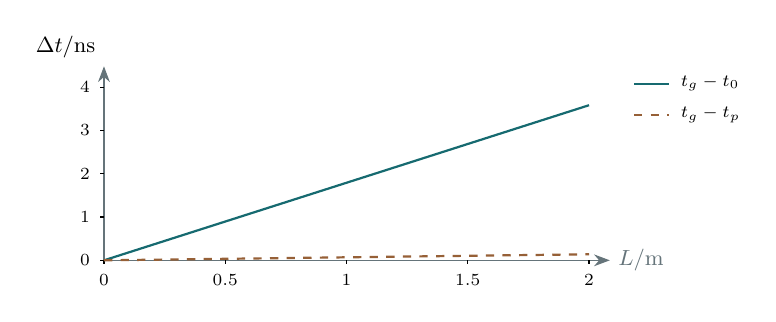
\begin{tikzpicture}[scale=.88,transform shape]
\draw[axis] (0,0.0)--(7.3,0.0) node[right] {$L/{\rm m}$};
\draw[axis] (0,0)--(0,2.8);
\node[above left] at (0,2.8) {$\Delta t/{\rm ns}$};
\draw[thin] (0.000000,0.0)--(0.000000,-0.06);\node[below,font=\scriptsize] at (0.000000,-0.08) {$ 0 $};
\draw[thin] (1.750000,0.0)--(1.750000,-0.06);\node[below,font=\scriptsize] at (1.750000,-0.08) {$ 0.5 $};
\draw[thin] (3.500000,0.0)--(3.500000,-0.06);\node[below,font=\scriptsize] at (3.500000,-0.08) {$ 1 $};
\draw[thin] (5.250000,0.0)--(5.250000,-0.06);\node[below,font=\scriptsize] at (5.250000,-0.08) {$ 1.5 $};
\draw[thin] (7.000000,0.0)--(7.000000,-0.06);\node[below,font=\scriptsize] at (7.000000,-0.08) {$ 2 $};
\draw[thin] (0,0.000000)--(-.06,0.000000);\node[left,font=\scriptsize] at (-.08,0.000000) {$ 0 $};
\draw[thin] (0,0.625000)--(-.06,0.625000);\node[left,font=\scriptsize] at (-.08,0.625000) {$ 1 $};
\draw[thin] (0,1.250000)--(-.06,1.250000);\node[left,font=\scriptsize] at (-.08,1.250000) {$ 2 $};
\draw[thin] (0,1.875000)--(-.06,1.875000);\node[left,font=\scriptsize] at (-.08,1.875000) {$ 3 $};
\draw[thin] (0,2.500000)--(-.06,2.500000);\node[left,font=\scriptsize] at (-.08,2.500000) {$ 4 $};
\draw[thick,color=accent] plot coordinates {(0.0000000,0.0000000) (0.0291667,0.0093273) (0.0583333,0.0186546) (0.0875000,0.0279819) (0.1166667,0.0373092) (0.1458333,0.0466365) (0.1750000,0.0559638) (0.2041667,0.0652912) (0.2333333,0.0746185) (0.2625000,0.0839458) (0.2916667,0.0932731) (0.3208333,0.1026004) (0.3500000,0.1119277) (0.3791667,0.1212550) (0.4083333,0.1305823) (0.4375000,0.1399096) (0.4666667,0.1492369) (0.4958333,0.1585642) (0.5250000,0.1678915) (0.5541667,0.1772188) (0.5833333,0.1865462) (0.6125000,0.1958735) (0.6416667,0.2052008) (0.6708333,0.2145281) (0.7000000,0.2238554) (0.7291667,0.2331827) (0.7583333,0.2425100) (0.7875000,0.2518373) (0.8166667,0.2611646) (0.8458333,0.2704919) (0.8750000,0.2798192) (0.9041667,0.2891465) (0.9333333,0.2984738) (0.9625000,0.3078012) (0.9916667,0.3171285) (1.0208333,0.3264558) (1.0500000,0.3357831) (1.0791667,0.3451104) (1.1083333,0.3544377) (1.1375000,0.3637650) (1.1666667,0.3730923) (1.1958333,0.3824196) (1.2250000,0.3917469) (1.2541667,0.4010742) (1.2833333,0.4104015) (1.3125000,0.4197288) (1.3416667,0.4290562) (1.3708333,0.4383835) (1.4000000,0.4477108) (1.4291667,0.4570381) (1.4583333,0.4663654) (1.4875000,0.4756927) (1.5166667,0.4850200) (1.5458333,0.4943473) (1.5750000,0.5036746) (1.6041667,0.5130019) (1.6333333,0.5223292) (1.6625000,0.5316565) (1.6916667,0.5409838) (1.7208333,0.5503112) (1.7500000,0.5596385) (1.7791667,0.5689658) (1.8083333,0.5782931) (1.8375000,0.5876204) (1.8666667,0.5969477) (1.8958333,0.6062750) (1.9250000,0.6156023) (1.9541667,0.6249296) (1.9833333,0.6342569) (2.0125000,0.6435842) (2.0416667,0.6529115) (2.0708333,0.6622388) (2.1000000,0.6715662) (2.1291667,0.6808935) (2.1583333,0.6902208) (2.1875000,0.6995481) (2.2166667,0.7088754) (2.2458333,0.7182027) (2.2750000,0.7275300) (2.3041667,0.7368573) (2.3333333,0.7461846) (2.3625000,0.7555119) (2.3916667,0.7648392) (2.4208333,0.7741665) (2.4500000,0.7834938) (2.4791667,0.7928212) (2.5083333,0.8021485) (2.5375000,0.8114758) (2.5666667,0.8208031) (2.5958333,0.8301304) (2.6250000,0.8394577) (2.6541667,0.8487850) (2.6833333,0.8581123) (2.7125000,0.8674396) (2.7416667,0.8767669) (2.7708333,0.8860942) (2.8000000,0.8954215) (2.8291667,0.9047489) (2.8583333,0.9140762) (2.8875000,0.9234035) (2.9166667,0.9327308) (2.9458333,0.9420581) (2.9750000,0.9513854) (3.0041667,0.9607127) (3.0333333,0.9700400) (3.0625000,0.9793673) (3.0916667,0.9886946) (3.1208333,0.9980219) (3.1500000,1.0073492) (3.1791667,1.0166765) (3.2083333,1.0260039) (3.2375000,1.0353312) (3.2666667,1.0446585) (3.2958333,1.0539858) (3.3250000,1.0633131) (3.3541667,1.0726404) (3.3833333,1.0819677) (3.4125000,1.0912950) (3.4416667,1.1006223) (3.4708333,1.1099496) (3.5000000,1.1192769) (3.5291667,1.1286042) (3.5583333,1.1379315) (3.5875000,1.1472589) (3.6166667,1.1565862) (3.6458333,1.1659135) (3.6750000,1.1752408) (3.7041667,1.1845681) (3.7333333,1.1938954) (3.7625000,1.2032227) (3.7916667,1.2125500) (3.8208333,1.2218773) (3.8500000,1.2312046) (3.8791667,1.2405319) (3.9083333,1.2498592) (3.9375000,1.2591865) (3.9666667,1.2685139) (3.9958333,1.2778412) (4.0250000,1.2871685) (4.0541667,1.2964958) (4.0833333,1.3058231) (4.1125000,1.3151504) (4.1416667,1.3244777) (4.1708333,1.3338050) (4.2000000,1.3431323) (4.2291667,1.3524596) (4.2583333,1.3617869) (4.2875000,1.3711142) (4.3166667,1.3804415) (4.3458333,1.3897689) (4.3750000,1.3990962) (4.4041667,1.4084235) (4.4333333,1.4177508) (4.4625000,1.4270781) (4.4916667,1.4364054) (4.5208333,1.4457327) (4.5500000,1.4550600) (4.5791667,1.4643873) (4.6083333,1.4737146) (4.6375000,1.4830419) (4.6666667,1.4923692) (4.6958333,1.5016965) (4.7250000,1.5110239) (4.7541667,1.5203512) (4.7833333,1.5296785) (4.8125000,1.5390058) (4.8416667,1.5483331) (4.8708333,1.5576604) (4.9000000,1.5669877) (4.9291667,1.5763150) (4.9583333,1.5856423) (4.9875000,1.5949696) (5.0166667,1.6042969) (5.0458333,1.6136242) (5.0750000,1.6229515) (5.1041667,1.6322789) (5.1333333,1.6416062) (5.1625000,1.6509335) (5.1916667,1.6602608) (5.2208333,1.6695881) (5.2500000,1.6789154) (5.2791667,1.6882427) (5.3083333,1.6975700) (5.3375000,1.7068973) (5.3666667,1.7162246) (5.3958333,1.7255519) (5.4250000,1.7348792) (5.4541667,1.7442065) (5.4833333,1.7535339) (5.5125000,1.7628612) (5.5416667,1.7721885) (5.5708333,1.7815158) (5.6000000,1.7908431) (5.6291667,1.8001704) (5.6583333,1.8094977) (5.6875000,1.8188250) (5.7166667,1.8281523) (5.7458333,1.8374796) (5.7750000,1.8468069) (5.8041667,1.8561342) (5.8333333,1.8654615) (5.8625000,1.8747889) (5.8916667,1.8841162) (5.9208333,1.8934435) (5.9500000,1.9027708) (5.9791667,1.9120981) (6.0083333,1.9214254) (6.0375000,1.9307527) (6.0666667,1.9400800) (6.0958333,1.9494073) (6.1250000,1.9587346) (6.1541667,1.9680619) (6.1833333,1.9773892) (6.2125000,1.9867165) (6.2416667,1.9960439) (6.2708333,2.0053712) (6.3000000,2.0146985) (6.3291667,2.0240258) (6.3583333,2.0333531) (6.3875000,2.0426804) (6.4166667,2.0520077) (6.4458333,2.0613350) (6.4750000,2.0706623) (6.5041667,2.0799896) (6.5333333,2.0893169) (6.5625000,2.0986442) (6.5916667,2.1079715) (6.6208333,2.1172989) (6.6500000,2.1266262) (6.6791667,2.1359535) (6.7083333,2.1452808) (6.7375000,2.1546081) (6.7666667,2.1639354) (6.7958333,2.1732627) (6.8250000,2.1825900) (6.8541667,2.1919173) (6.8833333,2.2012446) (6.9125000,2.2105719) (6.9416667,2.2198992) (6.9708333,2.2292265) (7.0000000,2.2385539)};
\draw[thick,color=accent] (7.65,2.55)--(8.15,2.55);\node[right,font=\scriptsize] at (8.2,2.55) {$t_g-t_0$};
\draw[thick,dashed,color=warm] plot coordinates {(0.0000000,0.0000000) (0.0291667,0.0003638) (0.0583333,0.0007275) (0.0875000,0.0010913) (0.1166667,0.0014551) (0.1458333,0.0018188) (0.1750000,0.0021826) (0.2041667,0.0025464) (0.2333333,0.0029101) (0.2625000,0.0032739) (0.2916667,0.0036377) (0.3208333,0.0040014) (0.3500000,0.0043652) (0.3791667,0.0047290) (0.4083333,0.0050927) (0.4375000,0.0054565) (0.4666667,0.0058203) (0.4958333,0.0061840) (0.5250000,0.0065478) (0.5541667,0.0069116) (0.5833333,0.0072753) (0.6125000,0.0076391) (0.6416667,0.0080029) (0.6708333,0.0083666) (0.7000000,0.0087304) (0.7291667,0.0090942) (0.7583333,0.0094579) (0.7875000,0.0098217) (0.8166667,0.0101854) (0.8458333,0.0105492) (0.8750000,0.0109130) (0.9041667,0.0112767) (0.9333333,0.0116405) (0.9625000,0.0120043) (0.9916667,0.0123680) (1.0208333,0.0127318) (1.0500000,0.0130956) (1.0791667,0.0134593) (1.1083333,0.0138231) (1.1375000,0.0141869) (1.1666667,0.0145506) (1.1958333,0.0149144) (1.2250000,0.0152782) (1.2541667,0.0156419) (1.2833333,0.0160057) (1.3125000,0.0163695) (1.3416667,0.0167332) (1.3708333,0.0170970) (1.4000000,0.0174608) (1.4291667,0.0178245) (1.4583333,0.0181883) (1.4875000,0.0185521) (1.5166667,0.0189158) (1.5458333,0.0192796) (1.5750000,0.0196434) (1.6041667,0.0200071) (1.6333333,0.0203709) (1.6625000,0.0207347) (1.6916667,0.0210984) (1.7208333,0.0214622) (1.7500000,0.0218260) (1.7791667,0.0221897) (1.8083333,0.0225535) (1.8375000,0.0229173) (1.8666667,0.0232810) (1.8958333,0.0236448) (1.9250000,0.0240086) (1.9541667,0.0243723) (1.9833333,0.0247361) (2.0125000,0.0250999) (2.0416667,0.0254636) (2.0708333,0.0258274) (2.1000000,0.0261912) (2.1291667,0.0265549) (2.1583333,0.0269187) (2.1875000,0.0272825) (2.2166667,0.0276462) (2.2458333,0.0280100) (2.2750000,0.0283738) (2.3041667,0.0287375) (2.3333333,0.0291013) (2.3625000,0.0294651) (2.3916667,0.0298288) (2.4208333,0.0301926) (2.4500000,0.0305563) (2.4791667,0.0309201) (2.5083333,0.0312839) (2.5375000,0.0316476) (2.5666667,0.0320114) (2.5958333,0.0323752) (2.6250000,0.0327389) (2.6541667,0.0331027) (2.6833333,0.0334665) (2.7125000,0.0338302) (2.7416667,0.0341940) (2.7708333,0.0345578) (2.8000000,0.0349215) (2.8291667,0.0352853) (2.8583333,0.0356491) (2.8875000,0.0360128) (2.9166667,0.0363766) (2.9458333,0.0367404) (2.9750000,0.0371041) (3.0041667,0.0374679) (3.0333333,0.0378317) (3.0625000,0.0381954) (3.0916667,0.0385592) (3.1208333,0.0389230) (3.1500000,0.0392867) (3.1791667,0.0396505) (3.2083333,0.0400143) (3.2375000,0.0403780) (3.2666667,0.0407418) (3.2958333,0.0411056) (3.3250000,0.0414693) (3.3541667,0.0418331) (3.3833333,0.0421969) (3.4125000,0.0425606) (3.4416667,0.0429244) (3.4708333,0.0432882) (3.5000000,0.0436519) (3.5291667,0.0440157) (3.5583333,0.0443795) (3.5875000,0.0447432) (3.6166667,0.0451070) (3.6458333,0.0454708) (3.6750000,0.0458345) (3.7041667,0.0461983) (3.7333333,0.0465621) (3.7625000,0.0469258) (3.7916667,0.0472896) (3.8208333,0.0476534) (3.8500000,0.0480171) (3.8791667,0.0483809) (3.9083333,0.0487447) (3.9375000,0.0491084) (3.9666667,0.0494722) (3.9958333,0.0498360) (4.0250000,0.0501997) (4.0541667,0.0505635) (4.0833333,0.0509272) (4.1125000,0.0512910) (4.1416667,0.0516548) (4.1708333,0.0520185) (4.2000000,0.0523823) (4.2291667,0.0527461) (4.2583333,0.0531098) (4.2875000,0.0534736) (4.3166667,0.0538374) (4.3458333,0.0542011) (4.3750000,0.0545649) (4.4041667,0.0549287) (4.4333333,0.0552924) (4.4625000,0.0556562) (4.4916667,0.0560200) (4.5208333,0.0563837) (4.5500000,0.0567475) (4.5791667,0.0571113) (4.6083333,0.0574750) (4.6375000,0.0578388) (4.6666667,0.0582026) (4.6958333,0.0585663) (4.7250000,0.0589301) (4.7541667,0.0592939) (4.7833333,0.0596576) (4.8125000,0.0600214) (4.8416667,0.0603852) (4.8708333,0.0607489) (4.9000000,0.0611127) (4.9291667,0.0614765) (4.9583333,0.0618402) (4.9875000,0.0622040) (5.0166667,0.0625678) (5.0458333,0.0629315) (5.0750000,0.0632953) (5.1041667,0.0636591) (5.1333333,0.0640228) (5.1625000,0.0643866) (5.1916667,0.0647504) (5.2208333,0.0651141) (5.2500000,0.0654779) (5.2791667,0.0658417) (5.3083333,0.0662054) (5.3375000,0.0665692) (5.3666667,0.0669330) (5.3958333,0.0672967) (5.4250000,0.0676605) (5.4541667,0.0680243) (5.4833333,0.0683880) (5.5125000,0.0687518) (5.5416667,0.0691156) (5.5708333,0.0694793) (5.6000000,0.0698431) (5.6291667,0.0702069) (5.6583333,0.0705706) (5.6875000,0.0709344) (5.7166667,0.0712981) (5.7458333,0.0716619) (5.7750000,0.0720257) (5.8041667,0.0723894) (5.8333333,0.0727532) (5.8625000,0.0731170) (5.8916667,0.0734807) (5.9208333,0.0738445) (5.9500000,0.0742083) (5.9791667,0.0745720) (6.0083333,0.0749358) (6.0375000,0.0752996) (6.0666667,0.0756633) (6.0958333,0.0760271) (6.1250000,0.0763909) (6.1541667,0.0767546) (6.1833333,0.0771184) (6.2125000,0.0774822) (6.2416667,0.0778459) (6.2708333,0.0782097) (6.3000000,0.0785735) (6.3291667,0.0789372) (6.3583333,0.0793010) (6.3875000,0.0796648) (6.4166667,0.0800285) (6.4458333,0.0803923) (6.4750000,0.0807561) (6.5041667,0.0811198) (6.5333333,0.0814836) (6.5625000,0.0818474) (6.5916667,0.0822111) (6.6208333,0.0825749) (6.6500000,0.0829387) (6.6791667,0.0833024) (6.7083333,0.0836662) (6.7375000,0.0840300) (6.7666667,0.0843937) (6.7958333,0.0847575) (6.8250000,0.0851213) (6.8541667,0.0854850) (6.8833333,0.0858488) (6.9125000,0.0862126) (6.9416667,0.0865763) (6.9708333,0.0869401) (7.0000000,0.0873039)};
\draw[thick,dashed,color=warm] (7.65,2.0999999999999996)--(8.15,2.0999999999999996);\node[right,font=\scriptsize] at (8.2,2.0999999999999996) {$t_g-t_p$};
\end{tikzpicture}
\figcaption{变图光5.1V3\quad 群延迟相对真空与相对相位面的差随长度线性增加}
\end{minipage}\end{center}
\item \textbf{二阶色散使高斯包络展宽。}设输入包络$A(t,0)=\exp[-t^2/(2T_0^2)]$，$T_0=100\,\mathrm{fs}$，$k''=50\,\mathrm{fs^2/mm}$。求不同长度的宽度，并说明频率端点群延迟差。

频谱传播相位二阶项为$\tfrac12k''L\Omega^2$。以群延迟后的时间$\tau=t-L/v_g$表示，高斯积分为
\[
 A(\tau,L)\propto\int_{-\infty}^{+\infty}
 e^{-(T_0^2-ik''L)\Omega^2/2-i\Omega\tau}\,\dd\Omega
 \propto\frac{\exp[-\tau^2/(2(T_0^2-ik''L))]}{\sqrt{T_0^2-ik''L}}.
\]
取模平方后，时间指数为$-T_0^2\tau^2/[T_0^4+(k''L)^2]$，故强度特征宽度为
\[
 T(L)=T_0\sqrt{1+(k''L/T_0^2)^2}.
\]
变图光5.1V4画出该宽度，$L=10\,\mathrm{mm}$时$T=100.1249\,\mathrm{fs}$，$L=1000\,\mathrm{mm}$时$T=509.9020\,\mathrm{fs}$。两频率相隔$\Delta\omega$的群延迟差为$\Delta t\simeq Lk''\Delta\omega$；它与脉宽相当时，频率成分在时间上明显分开，上式保留这一展宽。
\begin{center}\begin{minipage}{.98\linewidth}\centering
\begin{tikzpicture}[scale=.88,transform shape]
\draw[axis] (0,0.0)--(7.3,0.0) node[right] {$L/{\rm mm}$};
\draw[axis] (0,0)--(0,2.8);
\node[above left] at (0,2.8) {$T/{\rm fs}$};
\draw[thin] (0.000000,0.0)--(0.000000,-0.06);\node[below,font=\scriptsize] at (0.000000,-0.08) {$ 0 $};
\draw[thin] (1.400000,0.0)--(1.400000,-0.06);\node[below,font=\scriptsize] at (1.400000,-0.08) {$ 200 $};
\draw[thin] (3.500000,0.0)--(3.500000,-0.06);\node[below,font=\scriptsize] at (3.500000,-0.08) {$ 500 $};
\draw[thin] (7.000000,0.0)--(7.000000,-0.06);\node[below,font=\scriptsize] at (7.000000,-0.08) {$ 1000 $};
\draw[thin] (0,0.000000)--(-.06,0.000000);\node[left,font=\scriptsize] at (-.08,0.000000) {$ 0 $};
\draw[thin] (0,0.454545)--(-.06,0.454545);\node[left,font=\scriptsize] at (-.08,0.454545) {$ 100 $};
\draw[thin] (0,1.363636)--(-.06,1.363636);\node[left,font=\scriptsize] at (-.08,1.363636) {$ 300 $};
\draw[thin] (0,2.272727)--(-.06,2.272727);\node[left,font=\scriptsize] at (-.08,2.272727) {$ 500 $};
\draw[thick,color=accent] plot coordinates {(0.0000000,0.4545455) (0.0291667,0.4546441) (0.0583333,0.4549399) (0.0875000,0.4554324) (0.1166667,0.4561210) (0.1458333,0.4570049) (0.1750000,0.4580828) (0.2041667,0.4593535) (0.2333333,0.4608153) (0.2625000,0.4624665) (0.2916667,0.4643049) (0.3208333,0.4663285) (0.3500000,0.4685347) (0.3791667,0.4709211) (0.4083333,0.4734848) (0.4375000,0.4762231) (0.4666667,0.4791330) (0.4958333,0.4822113) (0.5250000,0.4854548) (0.5541667,0.4888602) (0.5833333,0.4924242) (0.6125000,0.4961434) (0.6416667,0.5000143) (0.6708333,0.5040335) (0.7000000,0.5081973) (0.7291667,0.5125022) (0.7583333,0.5169449) (0.7875000,0.5215216) (0.8166667,0.5262289) (0.8458333,0.5310634) (0.8750000,0.5360217) (0.9041667,0.5411002) (0.9333333,0.5462956) (0.9625000,0.5516048) (0.9916667,0.5570243) (1.0208333,0.5625510) (1.0500000,0.5681818) (1.0791667,0.5739136) (1.1083333,0.5797435) (1.1375000,0.5856684) (1.1666667,0.5916856) (1.1958333,0.5977922) (1.2250000,0.6039856) (1.2541667,0.6102630) (1.2833333,0.6166220) (1.3125000,0.6230600) (1.3416667,0.6295746) (1.3708333,0.6361635) (1.4000000,0.6428243) (1.4291667,0.6495549) (1.4583333,0.6563532) (1.4875000,0.6632169) (1.5166667,0.6701442) (1.5458333,0.6771330) (1.5750000,0.6841815) (1.6041667,0.6912879) (1.6333333,0.6984503) (1.6625000,0.7056672) (1.6916667,0.7129368) (1.7208333,0.7202575) (1.7500000,0.7276278) (1.7791667,0.7350462) (1.8083333,0.7425112) (1.8375000,0.7500215) (1.8666667,0.7575758) (1.8958333,0.7651726) (1.9250000,0.7728108) (1.9541667,0.7804892) (1.9833333,0.7882065) (2.0125000,0.7959617) (2.0416667,0.8037536) (2.0708333,0.8115812) (2.1000000,0.8194435) (2.1291667,0.8273394) (2.1583333,0.8352681) (2.1875000,0.8432285) (2.2166667,0.8512199) (2.2458333,0.8592413) (2.2750000,0.8672919) (2.3041667,0.8753709) (2.3333333,0.8834776) (2.3625000,0.8916111) (2.3916667,0.8997707) (2.4208333,0.9079558) (2.4500000,0.9161657) (2.4791667,0.9243996) (2.5083333,0.9326570) (2.5375000,0.9409372) (2.5666667,0.9492397) (2.5958333,0.9575638) (2.6250000,0.9659091) (2.6541667,0.9742749) (2.6833333,0.9826607) (2.7125000,0.9910661) (2.7416667,0.9994905) (2.7708333,1.0079335) (2.8000000,1.0163945) (2.8291667,1.0248732) (2.8583333,1.0333692) (2.8875000,1.0418819) (2.9166667,1.0504110) (2.9458333,1.0589560) (2.9750000,1.0675167) (3.0041667,1.0760926) (3.0333333,1.0846834) (3.0625000,1.0932887) (3.0916667,1.1019082) (3.1208333,1.1105415) (3.1500000,1.1191884) (3.1791667,1.1278485) (3.2083333,1.1365215) (3.2375000,1.1452071) (3.2666667,1.1539050) (3.2958333,1.1626150) (3.3250000,1.1713368) (3.3541667,1.1800702) (3.3833333,1.1888148) (3.4125000,1.1975704) (3.4416667,1.2063368) (3.4708333,1.2151138) (3.5000000,1.2239011) (3.5291667,1.2326985) (3.5583333,1.2415058) (3.5875000,1.2503228) (3.6166667,1.2591493) (3.6458333,1.2679850) (3.6750000,1.2768298) (3.7041667,1.2856836) (3.7333333,1.2945460) (3.7625000,1.3034170) (3.7916667,1.3122964) (3.8208333,1.3211839) (3.8500000,1.3300795) (3.8791667,1.3389830) (3.9083333,1.3478942) (3.9375000,1.3568129) (3.9666667,1.3657391) (3.9958333,1.3746726) (4.0250000,1.3836131) (4.0541667,1.3925607) (4.0833333,1.4015152) (4.1125000,1.4104763) (4.1416667,1.4194441) (4.1708333,1.4284183) (4.2000000,1.4373989) (4.2291667,1.4463858) (4.2583333,1.4553787) (4.2875000,1.4643777) (4.3166667,1.4733826) (4.3458333,1.4823933) (4.3750000,1.4914096) (4.4041667,1.5004316) (4.4333333,1.5094590) (4.4625000,1.5184918) (4.4916667,1.5275299) (4.5208333,1.5365732) (4.5500000,1.5456216) (4.5791667,1.5546751) (4.6083333,1.5637334) (4.6375000,1.5727967) (4.6666667,1.5818646) (4.6958333,1.5909373) (4.7250000,1.6000145) (4.7541667,1.6090963) (4.7833333,1.6181825) (4.8125000,1.6272731) (4.8416667,1.6363680) (4.8708333,1.6454671) (4.9000000,1.6545704) (4.9291667,1.6636778) (4.9583333,1.6727892) (4.9875000,1.6819046) (5.0166667,1.6910238) (5.0458333,1.7001469) (5.0750000,1.7092737) (5.1041667,1.7184043) (5.1333333,1.7275385) (5.1625000,1.7366763) (5.1916667,1.7458177) (5.2208333,1.7549625) (5.2500000,1.7641108) (5.2791667,1.7732624) (5.3083333,1.7824173) (5.3375000,1.7915756) (5.3666667,1.8007370) (5.3958333,1.8099016) (5.4250000,1.8190694) (5.4541667,1.8282402) (5.4833333,1.8374141) (5.5125000,1.8465909) (5.5416667,1.8557707) (5.5708333,1.8649534) (5.6000000,1.8741389) (5.6291667,1.8833273) (5.6583333,1.8925184) (5.6875000,1.9017123) (5.7166667,1.9109088) (5.7458333,1.9201080) (5.7750000,1.9293099) (5.8041667,1.9385143) (5.8333333,1.9477212) (5.8625000,1.9569307) (5.8916667,1.9661426) (5.9208333,1.9753570) (5.9500000,1.9845738) (5.9791667,1.9937929) (6.0083333,2.0030144) (6.0375000,2.0122382) (6.0666667,2.0214643) (6.0958333,2.0306926) (6.1250000,2.0399231) (6.1541667,2.0491558) (6.1833333,2.0583906) (6.2125000,2.0676276) (6.2416667,2.0768667) (6.2708333,2.0861078) (6.3000000,2.0953510) (6.3291667,2.1045962) (6.3583333,2.1138434) (6.3875000,2.1230925) (6.4166667,2.1323436) (6.4458333,2.1415966) (6.4750000,2.1508515) (6.5041667,2.1601082) (6.5333333,2.1693668) (6.5625000,2.1786272) (6.5916667,2.1878894) (6.6208333,2.1971534) (6.6500000,2.2064191) (6.6791667,2.2156865) (6.7083333,2.2249556) (6.7375000,2.2342264) (6.7666667,2.2434989) (6.7958333,2.2527730) (6.8250000,2.2620488) (6.8541667,2.2713261) (6.8833333,2.2806050) (6.9125000,2.2898855) (6.9416667,2.2991675) (6.9708333,2.3084511) (7.0000000,2.3177361)};
\end{tikzpicture}
\figcaption{变图光5.1V4\quad 二阶谱相位使高斯包络的时间宽度增加}
\end{minipage}\end{center}
\item \textbf{局部测量怎样校准拟合常数。}用$n_D$校准$A$而保留$B,C$，求校准前后$n,n_g$之差，并比较工作点两速度。

校准为$A_c=A+\Delta A$，其中$\Delta A=.0006734503$。对任意波长，$n_c-n_{\rm fit}=\Delta A$且$n'_c=n'_{\rm fit}$，故$n_{g,c}-n_{g,\rm fit}=\Delta A$。变图光5.1V5的两条差值线重合。工作点速度由未校准的$(1.9793794,1.9523884)\times10^8\,\mathrm{m/s}$变为$(1.9785003,1.9515331)\times10^8\,\mathrm{m/s}$，分别对应相速和群速。
\begin{center}\begin{minipage}{.98\linewidth}\centering
\begin{tikzpicture}[scale=.88,transform shape]
\draw[axis] (0,0.0)--(7.3,0.0) node[right] {$\lambda_0/{\rm nm}$};
\draw[axis] (0,0)--(0,2.8);
\node[above left] at (0,2.8) {$\text{折射率差}$};
\draw[thin] (0.000000,0.0)--(0.000000,-0.06);\node[below,font=\scriptsize] at (0.000000,-0.08) {$ 420 $};
\draw[thin] (3.118684,0.0)--(3.118684,-0.06);\node[below,font=\scriptsize] at (3.118684,-0.08) {$ 589.3 $};
\draw[thin] (7.000000,0.0)--(7.000000,-0.06);\node[below,font=\scriptsize] at (7.000000,-0.08) {$ 800 $};
\draw[thin] (0,0.000000)--(-.06,0.000000);\node[left,font=\scriptsize] at (-.08,0.000000) {$ 0 $};
\draw[thin] (0,1.250000)--(-.06,1.250000);\node[left,font=\scriptsize] at (-.08,1.250000) {$ 0.0004 $};
\draw[thin] (0,2.104531)--(-.06,2.104531);\node[left,font=\scriptsize] at (-.08,2.104531) {$ 0.00067345 $};
\draw[thin] (0,2.500000)--(-.06,2.500000);\node[left,font=\scriptsize] at (-.08,2.500000) {$ 0.0008 $};
\draw[thick,color=accent] plot coordinates {(0.0000000,2.1045322) (0.0291667,2.1045322) (0.0583333,2.1045322) (0.0875000,2.1045322) (0.1166667,2.1045322) (0.1458333,2.1045322) (0.1750000,2.1045322) (0.2041667,2.1045322) (0.2333333,2.1045322) (0.2625000,2.1045322) (0.2916667,2.1045322) (0.3208333,2.1045322) (0.3500000,2.1045322) (0.3791667,2.1045322) (0.4083333,2.1045322) (0.4375000,2.1045322) (0.4666667,2.1045322) (0.4958333,2.1045322) (0.5250000,2.1045322) (0.5541667,2.1045322) (0.5833333,2.1045322) (0.6125000,2.1045322) (0.6416667,2.1045322) (0.6708333,2.1045322) (0.7000000,2.1045322) (0.7291667,2.1045322) (0.7583333,2.1045322) (0.7875000,2.1045322) (0.8166667,2.1045322) (0.8458333,2.1045322) (0.8750000,2.1045322) (0.9041667,2.1045322) (0.9333333,2.1045322) (0.9625000,2.1045322) (0.9916667,2.1045322) (1.0208333,2.1045322) (1.0500000,2.1045322) (1.0791667,2.1045322) (1.1083333,2.1045322) (1.1375000,2.1045322) (1.1666667,2.1045322) (1.1958333,2.1045322) (1.2250000,2.1045322) (1.2541667,2.1045322) (1.2833333,2.1045322) (1.3125000,2.1045322) (1.3416667,2.1045322) (1.3708333,2.1045322) (1.4000000,2.1045322) (1.4291667,2.1045322) (1.4583333,2.1045322) (1.4875000,2.1045322) (1.5166667,2.1045322) (1.5458333,2.1045322) (1.5750000,2.1045322) (1.6041667,2.1045322) (1.6333333,2.1045322) (1.6625000,2.1045322) (1.6916667,2.1045322) (1.7208333,2.1045322) (1.7500000,2.1045322) (1.7791667,2.1045322) (1.8083333,2.1045322) (1.8375000,2.1045322) (1.8666667,2.1045322) (1.8958333,2.1045322) (1.9250000,2.1045322) (1.9541667,2.1045322) (1.9833333,2.1045322) (2.0125000,2.1045322) (2.0416667,2.1045322) (2.0708333,2.1045322) (2.1000000,2.1045322) (2.1291667,2.1045322) (2.1583333,2.1045322) (2.1875000,2.1045322) (2.2166667,2.1045322) (2.2458333,2.1045322) (2.2750000,2.1045322) (2.3041667,2.1045322) (2.3333333,2.1045322) (2.3625000,2.1045322) (2.3916667,2.1045322) (2.4208333,2.1045322) (2.4500000,2.1045322) (2.4791667,2.1045322) (2.5083333,2.1045322) (2.5375000,2.1045322) (2.5666667,2.1045322) (2.5958333,2.1045322) (2.6250000,2.1045322) (2.6541667,2.1045322) (2.6833333,2.1045322) (2.7125000,2.1045322) (2.7416667,2.1045322) (2.7708333,2.1045322) (2.8000000,2.1045322) (2.8291667,2.1045322) (2.8583333,2.1045322) (2.8875000,2.1045322) (2.9166667,2.1045322) (2.9458333,2.1045322) (2.9750000,2.1045322) (3.0041667,2.1045322) (3.0333333,2.1045322) (3.0625000,2.1045322) (3.0916667,2.1045322) (3.1208333,2.1045322) (3.1500000,2.1045322) (3.1791667,2.1045322) (3.2083333,2.1045322) (3.2375000,2.1045322) (3.2666667,2.1045322) (3.2958333,2.1045322) (3.3250000,2.1045322) (3.3541667,2.1045322) (3.3833333,2.1045322) (3.4125000,2.1045322) (3.4416667,2.1045322) (3.4708333,2.1045322) (3.5000000,2.1045322) (3.5291667,2.1045322) (3.5583333,2.1045322) (3.5875000,2.1045322) (3.6166667,2.1045322) (3.6458333,2.1045322) (3.6750000,2.1045322) (3.7041667,2.1045322) (3.7333333,2.1045322) (3.7625000,2.1045322) (3.7916667,2.1045322) (3.8208333,2.1045322) (3.8500000,2.1045322) (3.8791667,2.1045322) (3.9083333,2.1045322) (3.9375000,2.1045322) (3.9666667,2.1045322) (3.9958333,2.1045322) (4.0250000,2.1045322) (4.0541667,2.1045322) (4.0833333,2.1045322) (4.1125000,2.1045322) (4.1416667,2.1045322) (4.1708333,2.1045322) (4.2000000,2.1045322) (4.2291667,2.1045322) (4.2583333,2.1045322) (4.2875000,2.1045322) (4.3166667,2.1045322) (4.3458333,2.1045322) (4.3750000,2.1045322) (4.4041667,2.1045322) (4.4333333,2.1045322) (4.4625000,2.1045322) (4.4916667,2.1045322) (4.5208333,2.1045322) (4.5500000,2.1045322) (4.5791667,2.1045322) (4.6083333,2.1045322) (4.6375000,2.1045322) (4.6666667,2.1045322) (4.6958333,2.1045322) (4.7250000,2.1045322) (4.7541667,2.1045322) (4.7833333,2.1045322) (4.8125000,2.1045322) (4.8416667,2.1045322) (4.8708333,2.1045322) (4.9000000,2.1045322) (4.9291667,2.1045322) (4.9583333,2.1045322) (4.9875000,2.1045322) (5.0166667,2.1045322) (5.0458333,2.1045322) (5.0750000,2.1045322) (5.1041667,2.1045322) (5.1333333,2.1045322) (5.1625000,2.1045322) (5.1916667,2.1045322) (5.2208333,2.1045322) (5.2500000,2.1045322) (5.2791667,2.1045322) (5.3083333,2.1045322) (5.3375000,2.1045322) (5.3666667,2.1045322) (5.3958333,2.1045322) (5.4250000,2.1045322) (5.4541667,2.1045322) (5.4833333,2.1045322) (5.5125000,2.1045322) (5.5416667,2.1045322) (5.5708333,2.1045322) (5.6000000,2.1045322) (5.6291667,2.1045322) (5.6583333,2.1045322) (5.6875000,2.1045322) (5.7166667,2.1045322) (5.7458333,2.1045322) (5.7750000,2.1045322) (5.8041667,2.1045322) (5.8333333,2.1045322) (5.8625000,2.1045322) (5.8916667,2.1045322) (5.9208333,2.1045322) (5.9500000,2.1045322) (5.9791667,2.1045322) (6.0083333,2.1045322) (6.0375000,2.1045322) (6.0666667,2.1045322) (6.0958333,2.1045322) (6.1250000,2.1045322) (6.1541667,2.1045322) (6.1833333,2.1045322) (6.2125000,2.1045322) (6.2416667,2.1045322) (6.2708333,2.1045322) (6.3000000,2.1045322) (6.3291667,2.1045322) (6.3583333,2.1045322) (6.3875000,2.1045322) (6.4166667,2.1045322) (6.4458333,2.1045322) (6.4750000,2.1045322) (6.5041667,2.1045322) (6.5333333,2.1045322) (6.5625000,2.1045322) (6.5916667,2.1045322) (6.6208333,2.1045322) (6.6500000,2.1045322) (6.6791667,2.1045322) (6.7083333,2.1045322) (6.7375000,2.1045322) (6.7666667,2.1045322) (6.7958333,2.1045322) (6.8250000,2.1045322) (6.8541667,2.1045322) (6.8833333,2.1045322) (6.9125000,2.1045322) (6.9416667,2.1045322) (6.9708333,2.1045322) (7.0000000,2.1045322)};
\draw[thick,color=accent] (7.65,2.55)--(8.15,2.55);\node[right,font=\scriptsize] at (8.2,2.55) {$n_c-n_{\rm fit}$};
\draw[thick,dashed,color=warm] plot coordinates {(0.0000000,2.1045322) (0.0291667,2.1045322) (0.0583333,2.1045322) (0.0875000,2.1045322) (0.1166667,2.1045322) (0.1458333,2.1045322) (0.1750000,2.1045322) (0.2041667,2.1045322) (0.2333333,2.1045322) (0.2625000,2.1045322) (0.2916667,2.1045322) (0.3208333,2.1045322) (0.3500000,2.1045322) (0.3791667,2.1045322) (0.4083333,2.1045322) (0.4375000,2.1045322) (0.4666667,2.1045322) (0.4958333,2.1045322) (0.5250000,2.1045322) (0.5541667,2.1045322) (0.5833333,2.1045322) (0.6125000,2.1045322) (0.6416667,2.1045322) (0.6708333,2.1045322) (0.7000000,2.1045322) (0.7291667,2.1045322) (0.7583333,2.1045322) (0.7875000,2.1045322) (0.8166667,2.1045322) (0.8458333,2.1045322) (0.8750000,2.1045322) (0.9041667,2.1045322) (0.9333333,2.1045322) (0.9625000,2.1045322) (0.9916667,2.1045322) (1.0208333,2.1045322) (1.0500000,2.1045322) (1.0791667,2.1045322) (1.1083333,2.1045322) (1.1375000,2.1045322) (1.1666667,2.1045322) (1.1958333,2.1045322) (1.2250000,2.1045322) (1.2541667,2.1045322) (1.2833333,2.1045322) (1.3125000,2.1045322) (1.3416667,2.1045322) (1.3708333,2.1045322) (1.4000000,2.1045322) (1.4291667,2.1045322) (1.4583333,2.1045322) (1.4875000,2.1045322) (1.5166667,2.1045322) (1.5458333,2.1045322) (1.5750000,2.1045322) (1.6041667,2.1045322) (1.6333333,2.1045322) (1.6625000,2.1045322) (1.6916667,2.1045322) (1.7208333,2.1045322) (1.7500000,2.1045322) (1.7791667,2.1045322) (1.8083333,2.1045322) (1.8375000,2.1045322) (1.8666667,2.1045322) (1.8958333,2.1045322) (1.9250000,2.1045322) (1.9541667,2.1045322) (1.9833333,2.1045322) (2.0125000,2.1045322) (2.0416667,2.1045322) (2.0708333,2.1045322) (2.1000000,2.1045322) (2.1291667,2.1045322) (2.1583333,2.1045322) (2.1875000,2.1045322) (2.2166667,2.1045322) (2.2458333,2.1045322) (2.2750000,2.1045322) (2.3041667,2.1045322) (2.3333333,2.1045322) (2.3625000,2.1045322) (2.3916667,2.1045322) (2.4208333,2.1045322) (2.4500000,2.1045322) (2.4791667,2.1045322) (2.5083333,2.1045322) (2.5375000,2.1045322) (2.5666667,2.1045322) (2.5958333,2.1045322) (2.6250000,2.1045322) (2.6541667,2.1045322) (2.6833333,2.1045322) (2.7125000,2.1045322) (2.7416667,2.1045322) (2.7708333,2.1045322) (2.8000000,2.1045322) (2.8291667,2.1045322) (2.8583333,2.1045322) (2.8875000,2.1045322) (2.9166667,2.1045322) (2.9458333,2.1045322) (2.9750000,2.1045322) (3.0041667,2.1045322) (3.0333333,2.1045322) (3.0625000,2.1045322) (3.0916667,2.1045322) (3.1208333,2.1045322) (3.1500000,2.1045322) (3.1791667,2.1045322) (3.2083333,2.1045322) (3.2375000,2.1045322) (3.2666667,2.1045322) (3.2958333,2.1045322) (3.3250000,2.1045322) (3.3541667,2.1045322) (3.3833333,2.1045322) (3.4125000,2.1045322) (3.4416667,2.1045322) (3.4708333,2.1045322) (3.5000000,2.1045322) (3.5291667,2.1045322) (3.5583333,2.1045322) (3.5875000,2.1045322) (3.6166667,2.1045322) (3.6458333,2.1045322) (3.6750000,2.1045322) (3.7041667,2.1045322) (3.7333333,2.1045322) (3.7625000,2.1045322) (3.7916667,2.1045322) (3.8208333,2.1045322) (3.8500000,2.1045322) (3.8791667,2.1045322) (3.9083333,2.1045322) (3.9375000,2.1045322) (3.9666667,2.1045322) (3.9958333,2.1045322) (4.0250000,2.1045322) (4.0541667,2.1045322) (4.0833333,2.1045322) (4.1125000,2.1045322) (4.1416667,2.1045322) (4.1708333,2.1045322) (4.2000000,2.1045322) (4.2291667,2.1045322) (4.2583333,2.1045322) (4.2875000,2.1045322) (4.3166667,2.1045322) (4.3458333,2.1045322) (4.3750000,2.1045322) (4.4041667,2.1045322) (4.4333333,2.1045322) (4.4625000,2.1045322) (4.4916667,2.1045322) (4.5208333,2.1045322) (4.5500000,2.1045322) (4.5791667,2.1045322) (4.6083333,2.1045322) (4.6375000,2.1045322) (4.6666667,2.1045322) (4.6958333,2.1045322) (4.7250000,2.1045322) (4.7541667,2.1045322) (4.7833333,2.1045322) (4.8125000,2.1045322) (4.8416667,2.1045322) (4.8708333,2.1045322) (4.9000000,2.1045322) (4.9291667,2.1045322) (4.9583333,2.1045322) (4.9875000,2.1045322) (5.0166667,2.1045322) (5.0458333,2.1045322) (5.0750000,2.1045322) (5.1041667,2.1045322) (5.1333333,2.1045322) (5.1625000,2.1045322) (5.1916667,2.1045322) (5.2208333,2.1045322) (5.2500000,2.1045322) (5.2791667,2.1045322) (5.3083333,2.1045322) (5.3375000,2.1045322) (5.3666667,2.1045322) (5.3958333,2.1045322) (5.4250000,2.1045322) (5.4541667,2.1045322) (5.4833333,2.1045322) (5.5125000,2.1045322) (5.5416667,2.1045322) (5.5708333,2.1045322) (5.6000000,2.1045322) (5.6291667,2.1045322) (5.6583333,2.1045322) (5.6875000,2.1045322) (5.7166667,2.1045322) (5.7458333,2.1045322) (5.7750000,2.1045322) (5.8041667,2.1045322) (5.8333333,2.1045322) (5.8625000,2.1045322) (5.8916667,2.1045322) (5.9208333,2.1045322) (5.9500000,2.1045322) (5.9791667,2.1045322) (6.0083333,2.1045322) (6.0375000,2.1045322) (6.0666667,2.1045322) (6.0958333,2.1045322) (6.1250000,2.1045322) (6.1541667,2.1045322) (6.1833333,2.1045322) (6.2125000,2.1045322) (6.2416667,2.1045322) (6.2708333,2.1045322) (6.3000000,2.1045322) (6.3291667,2.1045322) (6.3583333,2.1045322) (6.3875000,2.1045322) (6.4166667,2.1045322) (6.4458333,2.1045322) (6.4750000,2.1045322) (6.5041667,2.1045322) (6.5333333,2.1045322) (6.5625000,2.1045322) (6.5916667,2.1045322) (6.6208333,2.1045322) (6.6500000,2.1045322) (6.6791667,2.1045322) (6.7083333,2.1045322) (6.7375000,2.1045322) (6.7666667,2.1045322) (6.7958333,2.1045322) (6.8250000,2.1045322) (6.8541667,2.1045322) (6.8833333,2.1045322) (6.9125000,2.1045322) (6.9416667,2.1045322) (6.9708333,2.1045322) (7.0000000,2.1045322)};
\draw[thick,dashed,color=warm] (7.65,2.0999999999999996)--(8.15,2.0999999999999996);\node[right,font=\scriptsize] at (8.2,2.0999999999999996) {$n_{g,c}-n_{g,\rm fit}$};
\end{tikzpicture}
\figcaption{变图光5.1V5\quad 常数项校准使相位和群折射率同量平移}
\end{minipage}\end{center}
\item \textbf{由介质内波长使用Rayleigh关系。}在589.3nm处求$\lambda_m$，并用链式导数证明$v_p-\lambda_m\dd v_p/\dd\lambda_m$给出完整群速。

由$\lambda_m=\lambda_0/n_D$得$\lambda_m=388.6434\,\mathrm{nm}$。又有$\dd\lambda_m/\dd\lambda_0=n_g/n^2$，而$\dd v_p/\dd\lambda_0=-cn'/n^2$，所以
\[
 v_p-\lambda_m\frac{\dd v_p}{\dd\lambda_m}
 =\frac cn+\frac{c\lambda_0n'}{nn_g}
 =\frac{c(n_g+\lambda_0n')}{nn_g}=\frac c{n_g}.
\]
变图光5.1V6的Rayleigh计算与群折射率计算逐点重合，工作点为$1.9515331\times10^8\,\mathrm{m/s}$。自变量转换保留了$n_g$分母，连接两种等价表达。
\begin{center}\begin{minipage}{.98\linewidth}\centering
\begin{tikzpicture}[scale=.88,transform shape]
\draw[axis] (0,0)--(7.3,0) node[right] {$\lambda_0/{\rm nm}$};
\draw[axis] (0,0)--(0,2.8);
\node[above left] at (0,2.8) {$v_g/(10^8{\rm m/s})$};
\draw[thin] (0.000000,0)--(0.000000,-0.06);\node[below,font=\scriptsize] at (0.000000,-0.08) {$ 420 $};
\draw[thin] (3.118684,0)--(3.118684,-0.06);\node[below,font=\scriptsize] at (3.118684,-0.08) {$ 589.3 $};
\draw[thin] (7.000000,0)--(7.000000,-0.06);\node[below,font=\scriptsize] at (7.000000,-0.08) {$ 800 $};
\draw[thin] (0,0.000000)--(-.06,0.000000);\node[left,font=\scriptsize] at (-.08,0.000000) {$ 1.9 $};
\draw[thin] (0,1.136364)--(-.06,1.136364);\node[left,font=\scriptsize] at (-.08,1.136364) {$ 1.95 $};
\draw[thin] (0,2.272727)--(-.06,2.272727);\node[left,font=\scriptsize] at (-.08,2.272727) {$ 2 $};
\draw[thick,color=accent] plot coordinates {(0.0000000,0.5849142) (0.0291667,0.5914558) (0.0583333,0.5979953) (0.0875000,0.6045315) (0.1166667,0.6110631) (0.1458333,0.6175891) (0.1750000,0.6241083) (0.2041667,0.6306198) (0.2333333,0.6371226) (0.2625000,0.6436157) (0.2916667,0.6500981) (0.3208333,0.6565690) (0.3500000,0.6630277) (0.3791667,0.6694732) (0.4083333,0.6759048) (0.4375000,0.6823218) (0.4666667,0.6887234) (0.4958333,0.6951091) (0.5250000,0.7014781) (0.5541667,0.7078299) (0.5833333,0.7141638) (0.6125000,0.7204793) (0.6416667,0.7267759) (0.6708333,0.7330531) (0.7000000,0.7393104) (0.7291667,0.7455473) (0.7583333,0.7517633) (0.7875000,0.7579582) (0.8166667,0.7641314) (0.8458333,0.7702826) (0.8750000,0.7764115) (0.9041667,0.7825176) (0.9333333,0.7886008) (0.9625000,0.7946606) (0.9916667,0.8006968) (1.0208333,0.8067092) (1.0500000,0.8126974) (1.0791667,0.8186613) (1.1083333,0.8246005) (1.1375000,0.8305150) (1.1666667,0.8364045) (1.1958333,0.8422688) (1.2250000,0.8481077) (1.2541667,0.8539211) (1.2833333,0.8597089) (1.3125000,0.8654708) (1.3416667,0.8712068) (1.3708333,0.8769168) (1.4000000,0.8826007) (1.4291667,0.8882582) (1.4583333,0.8938895) (1.4875000,0.8994944) (1.5166667,0.9050727) (1.5458333,0.9106245) (1.5750000,0.9161498) (1.6041667,0.9216484) (1.6333333,0.9271203) (1.6625000,0.9325655) (1.6916667,0.9379840) (1.7208333,0.9433757) (1.7500000,0.9487406) (1.7791667,0.9540788) (1.8083333,0.9593903) (1.8375000,0.9646749) (1.8666667,0.9699328) (1.8958333,0.9751640) (1.9250000,0.9803685) (1.9541667,0.9855463) (1.9833333,0.9906975) (2.0125000,0.9958220) (2.0416667,1.0009199) (2.0708333,1.0059914) (2.1000000,1.0110363) (2.1291667,1.0160548) (2.1583333,1.0210470) (2.1875000,1.0260128) (2.2166667,1.0309524) (2.2458333,1.0358657) (2.2750000,1.0407530) (2.3041667,1.0456142) (2.3333333,1.0504495) (2.3625000,1.0552588) (2.3916667,1.0600424) (2.4208333,1.0648002) (2.4500000,1.0695323) (2.4791667,1.0742389) (2.5083333,1.0789200) (2.5375000,1.0835757) (2.5666667,1.0882062) (2.5958333,1.0928114) (2.6250000,1.0973916) (2.6541667,1.1019467) (2.6833333,1.1064770) (2.7125000,1.1109824) (2.7416667,1.1154631) (2.7708333,1.1199193) (2.8000000,1.1243509) (2.8291667,1.1287582) (2.8583333,1.1331412) (2.8875000,1.1375000) (2.9166667,1.1418348) (2.9458333,1.1461456) (2.9750000,1.1504325) (3.0041667,1.1546958) (3.0333333,1.1589354) (3.0625000,1.1631515) (3.0916667,1.1673443) (3.1208333,1.1715137) (3.1500000,1.1756600) (3.1791667,1.1797833) (3.2083333,1.1838837) (3.2375000,1.1879612) (3.2666667,1.1920160) (3.2958333,1.1960483) (3.3250000,1.2000581) (3.3541667,1.2040456) (3.3833333,1.2080108) (3.4125000,1.2119540) (3.4416667,1.2158751) (3.4708333,1.2197744) (3.5000000,1.2236520) (3.5291667,1.2275079) (3.5583333,1.2313423) (3.5875000,1.2351553) (3.6166667,1.2389470) (3.6458333,1.2427176) (3.6750000,1.2464672) (3.7041667,1.2501958) (3.7333333,1.2539037) (3.7625000,1.2575908) (3.7916667,1.2612574) (3.8208333,1.2649036) (3.8500000,1.2685294) (3.8791667,1.2721350) (3.9083333,1.2757205) (3.9375000,1.2792861) (3.9666667,1.2828318) (3.9958333,1.2863577) (4.0250000,1.2898641) (4.0541667,1.2933509) (4.0833333,1.2968183) (4.1125000,1.3002665) (4.1416667,1.3036955) (4.1708333,1.3071054) (4.2000000,1.3104964) (4.2291667,1.3138686) (4.2583333,1.3172221) (4.2875000,1.3205570) (4.3166667,1.3238734) (4.3458333,1.3271715) (4.3750000,1.3304513) (4.4041667,1.3337129) (4.4333333,1.3369565) (4.4625000,1.3401822) (4.4916667,1.3433901) (4.5208333,1.3465802) (4.5500000,1.3497528) (4.5791667,1.3529079) (4.6083333,1.3560456) (4.6375000,1.3591660) (4.6666667,1.3622693) (4.6958333,1.3653555) (4.7250000,1.3684247) (4.7541667,1.3714772) (4.7833333,1.3745128) (4.8125000,1.3775319) (4.8416667,1.3805343) (4.8708333,1.3835204) (4.9000000,1.3864901) (4.9291667,1.3894437) (4.9583333,1.3923810) (4.9875000,1.3953024) (5.0166667,1.3982079) (5.0458333,1.4010975) (5.0750000,1.4039714) (5.1041667,1.4068297) (5.1333333,1.4096724) (5.1625000,1.4124997) (5.1916667,1.4153117) (5.2208333,1.4181085) (5.2500000,1.4208901) (5.2791667,1.4236567) (5.3083333,1.4264084) (5.3375000,1.4291452) (5.3666667,1.4318672) (5.3958333,1.4345746) (5.4250000,1.4372674) (5.4541667,1.4399457) (5.4833333,1.4426096) (5.5125000,1.4452593) (5.5416667,1.4478947) (5.5708333,1.4505160) (5.6000000,1.4531233) (5.6291667,1.4557167) (5.6583333,1.4582962) (5.6875000,1.4608620) (5.7166667,1.4634141) (5.7458333,1.4659526) (5.7750000,1.4684776) (5.8041667,1.4709892) (5.8333333,1.4734874) (5.8625000,1.4759725) (5.8916667,1.4784443) (5.9208333,1.4809031) (5.9500000,1.4833489) (5.9791667,1.4857818) (6.0083333,1.4882019) (6.0375000,1.4906092) (6.0666667,1.4930038) (6.0958333,1.4953859) (6.1250000,1.4977554) (6.1541667,1.5001126) (6.1833333,1.5024574) (6.2125000,1.5047899) (6.2416667,1.5071102) (6.2708333,1.5094184) (6.3000000,1.5117146) (6.3291667,1.5139988) (6.3583333,1.5162712) (6.3875000,1.5185317) (6.4166667,1.5207805) (6.4458333,1.5230176) (6.4750000,1.5252432) (6.5041667,1.5274572) (6.5333333,1.5296598) (6.5625000,1.5318510) (6.5916667,1.5340310) (6.6208333,1.5361997) (6.6500000,1.5383572) (6.6791667,1.5405037) (6.7083333,1.5426392) (6.7375000,1.5447637) (6.7666667,1.5468773) (6.7958333,1.5489801) (6.8250000,1.5510722) (6.8541667,1.5531536) (6.8833333,1.5552244) (6.9125000,1.5572847) (6.9416667,1.5593345) (6.9708333,1.5613739) (7.0000000,1.5634030)};
\draw[thick,color=accent] (7.65,2.55)--(8.15,2.55);\node[right,font=\scriptsize] at (8.2,2.55) {$c/n_g$};
\draw[thick,dashed,color=warm] plot coordinates {(0.0000000,0.5849142) (0.0291667,0.5914558) (0.0583333,0.5979953) (0.0875000,0.6045315) (0.1166667,0.6110631) (0.1458333,0.6175891) (0.1750000,0.6241083) (0.2041667,0.6306198) (0.2333333,0.6371226) (0.2625000,0.6436157) (0.2916667,0.6500981) (0.3208333,0.6565690) (0.3500000,0.6630277) (0.3791667,0.6694732) (0.4083333,0.6759048) (0.4375000,0.6823218) (0.4666667,0.6887234) (0.4958333,0.6951091) (0.5250000,0.7014781) (0.5541667,0.7078299) (0.5833333,0.7141638) (0.6125000,0.7204793) (0.6416667,0.7267759) (0.6708333,0.7330531) (0.7000000,0.7393104) (0.7291667,0.7455473) (0.7583333,0.7517633) (0.7875000,0.7579582) (0.8166667,0.7641314) (0.8458333,0.7702826) (0.8750000,0.7764115) (0.9041667,0.7825176) (0.9333333,0.7886008) (0.9625000,0.7946606) (0.9916667,0.8006968) (1.0208333,0.8067092) (1.0500000,0.8126974) (1.0791667,0.8186613) (1.1083333,0.8246005) (1.1375000,0.8305150) (1.1666667,0.8364045) (1.1958333,0.8422688) (1.2250000,0.8481077) (1.2541667,0.8539211) (1.2833333,0.8597089) (1.3125000,0.8654708) (1.3416667,0.8712068) (1.3708333,0.8769168) (1.4000000,0.8826007) (1.4291667,0.8882582) (1.4583333,0.8938895) (1.4875000,0.8994944) (1.5166667,0.9050727) (1.5458333,0.9106245) (1.5750000,0.9161498) (1.6041667,0.9216484) (1.6333333,0.9271203) (1.6625000,0.9325655) (1.6916667,0.9379840) (1.7208333,0.9433757) (1.7500000,0.9487406) (1.7791667,0.9540788) (1.8083333,0.9593903) (1.8375000,0.9646749) (1.8666667,0.9699328) (1.8958333,0.9751640) (1.9250000,0.9803685) (1.9541667,0.9855463) (1.9833333,0.9906975) (2.0125000,0.9958220) (2.0416667,1.0009199) (2.0708333,1.0059914) (2.1000000,1.0110363) (2.1291667,1.0160548) (2.1583333,1.0210470) (2.1875000,1.0260128) (2.2166667,1.0309524) (2.2458333,1.0358657) (2.2750000,1.0407530) (2.3041667,1.0456142) (2.3333333,1.0504495) (2.3625000,1.0552588) (2.3916667,1.0600424) (2.4208333,1.0648002) (2.4500000,1.0695323) (2.4791667,1.0742389) (2.5083333,1.0789200) (2.5375000,1.0835757) (2.5666667,1.0882062) (2.5958333,1.0928114) (2.6250000,1.0973916) (2.6541667,1.1019467) (2.6833333,1.1064770) (2.7125000,1.1109824) (2.7416667,1.1154631) (2.7708333,1.1199193) (2.8000000,1.1243509) (2.8291667,1.1287582) (2.8583333,1.1331412) (2.8875000,1.1375000) (2.9166667,1.1418348) (2.9458333,1.1461456) (2.9750000,1.1504325) (3.0041667,1.1546958) (3.0333333,1.1589354) (3.0625000,1.1631515) (3.0916667,1.1673443) (3.1208333,1.1715137) (3.1500000,1.1756600) (3.1791667,1.1797833) (3.2083333,1.1838837) (3.2375000,1.1879612) (3.2666667,1.1920160) (3.2958333,1.1960483) (3.3250000,1.2000581) (3.3541667,1.2040456) (3.3833333,1.2080108) (3.4125000,1.2119540) (3.4416667,1.2158751) (3.4708333,1.2197744) (3.5000000,1.2236520) (3.5291667,1.2275079) (3.5583333,1.2313423) (3.5875000,1.2351553) (3.6166667,1.2389470) (3.6458333,1.2427176) (3.6750000,1.2464672) (3.7041667,1.2501958) (3.7333333,1.2539037) (3.7625000,1.2575908) (3.7916667,1.2612574) (3.8208333,1.2649036) (3.8500000,1.2685294) (3.8791667,1.2721350) (3.9083333,1.2757205) (3.9375000,1.2792861) (3.9666667,1.2828318) (3.9958333,1.2863577) (4.0250000,1.2898641) (4.0541667,1.2933509) (4.0833333,1.2968183) (4.1125000,1.3002665) (4.1416667,1.3036955) (4.1708333,1.3071054) (4.2000000,1.3104964) (4.2291667,1.3138686) (4.2583333,1.3172221) (4.2875000,1.3205570) (4.3166667,1.3238734) (4.3458333,1.3271715) (4.3750000,1.3304513) (4.4041667,1.3337129) (4.4333333,1.3369565) (4.4625000,1.3401822) (4.4916667,1.3433901) (4.5208333,1.3465802) (4.5500000,1.3497528) (4.5791667,1.3529079) (4.6083333,1.3560456) (4.6375000,1.3591660) (4.6666667,1.3622693) (4.6958333,1.3653555) (4.7250000,1.3684247) (4.7541667,1.3714772) (4.7833333,1.3745128) (4.8125000,1.3775319) (4.8416667,1.3805343) (4.8708333,1.3835204) (4.9000000,1.3864901) (4.9291667,1.3894437) (4.9583333,1.3923810) (4.9875000,1.3953024) (5.0166667,1.3982079) (5.0458333,1.4010975) (5.0750000,1.4039714) (5.1041667,1.4068297) (5.1333333,1.4096724) (5.1625000,1.4124997) (5.1916667,1.4153117) (5.2208333,1.4181085) (5.2500000,1.4208901) (5.2791667,1.4236567) (5.3083333,1.4264084) (5.3375000,1.4291452) (5.3666667,1.4318672) (5.3958333,1.4345746) (5.4250000,1.4372674) (5.4541667,1.4399457) (5.4833333,1.4426096) (5.5125000,1.4452593) (5.5416667,1.4478947) (5.5708333,1.4505160) (5.6000000,1.4531233) (5.6291667,1.4557167) (5.6583333,1.4582962) (5.6875000,1.4608620) (5.7166667,1.4634141) (5.7458333,1.4659526) (5.7750000,1.4684776) (5.8041667,1.4709892) (5.8333333,1.4734874) (5.8625000,1.4759725) (5.8916667,1.4784443) (5.9208333,1.4809031) (5.9500000,1.4833489) (5.9791667,1.4857818) (6.0083333,1.4882019) (6.0375000,1.4906092) (6.0666667,1.4930038) (6.0958333,1.4953859) (6.1250000,1.4977554) (6.1541667,1.5001126) (6.1833333,1.5024574) (6.2125000,1.5047899) (6.2416667,1.5071102) (6.2708333,1.5094184) (6.3000000,1.5117146) (6.3291667,1.5139988) (6.3583333,1.5162712) (6.3875000,1.5185317) (6.4166667,1.5207805) (6.4458333,1.5230176) (6.4750000,1.5252432) (6.5041667,1.5274572) (6.5333333,1.5296598) (6.5625000,1.5318510) (6.5916667,1.5340310) (6.6208333,1.5361997) (6.6500000,1.5383572) (6.6791667,1.5405037) (6.7083333,1.5426392) (6.7375000,1.5447637) (6.7666667,1.5468773) (6.7958333,1.5489801) (6.8250000,1.5510722) (6.8541667,1.5531536) (6.8833333,1.5552244) (6.9125000,1.5572847) (6.9416667,1.5593345) (6.9708333,1.5613739) (7.0000000,1.5634030)};
\draw[thick,dashed,color=warm] (7.65,2.0999999999999996)--(8.15,2.0999999999999996);\node[right,font=\scriptsize] at (8.2,2.0999999999999996) {$\mathrm{Rayleigh}$};
\end{tikzpicture}
\figcaption{变图光5.1V6\quad 介质内波长的链式求导与完整群折射率结果重合}
\end{minipage}\end{center}
\item \textbf{局部斜率为正。}设$n(\lambda_D)=1.51630$，$\lambda_D=589.3\,\mathrm{nm}$，局部导数$s=2.0\times10^{-5}\,\mathrm{nm^{-1}}$。比较两速度。

群折射率为$n_g=n_D-\lambda_Ds=1.504514$，于是$v_g=1.9939994\times10^8\,\mathrm{m/s}$，相速仍为$1.9785003\times10^8\,\mathrm{m/s}$。变图光5.1V7随局部斜率$s$画群速，$s=0$时与相速相交；该给定局部透明窄带模型中，正斜率使$n_g<n_D$，群速较大，二者仍小于$c$。
\begin{center}\begin{minipage}{.98\linewidth}\centering
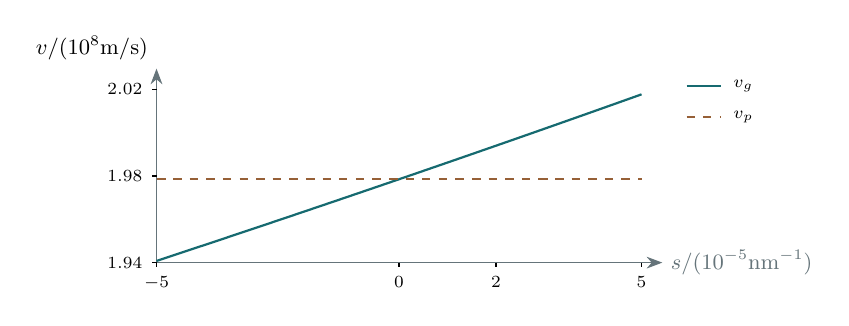
\begin{tikzpicture}[scale=.88,transform shape]
\draw[axis] (0,0)--(7.3,0) node[right] {$s/(10^{-5}{\rm nm^{-1}})$};
\draw[axis] (0,0)--(0,2.8);
\node[above left] at (0,2.8) {$v/(10^8{\rm m/s})$};
\draw[thin] (0.000000,0)--(0.000000,-0.06);\node[below,font=\scriptsize] at (0.000000,-0.08) {$ -5 $};
\draw[thin] (3.500000,0)--(3.500000,-0.06);\node[below,font=\scriptsize] at (3.500000,-0.08) {$ 0 $};
\draw[thin] (4.900000,0)--(4.900000,-0.06);\node[below,font=\scriptsize] at (4.900000,-0.08) {$ 2 $};
\draw[thin] (7.000000,0)--(7.000000,-0.06);\node[below,font=\scriptsize] at (7.000000,-0.08) {$ 5 $};
\draw[thin] (0,0.000000)--(-.06,0.000000);\node[left,font=\scriptsize] at (-.08,0.000000) {$ 1.94 $};
\draw[thin] (0,1.250000)--(-.06,1.250000);\node[left,font=\scriptsize] at (-.08,1.250000) {$ 1.98 $};
\draw[thin] (0,2.500000)--(-.06,2.500000);\node[left,font=\scriptsize] at (-.08,2.500000) {$ 2.02 $};
\draw[thick,color=accent] plot coordinates {(0.0000000,0.0245813) (0.0291667,0.0342169) (0.0583333,0.0438555) (0.0875000,0.0534972) (0.1166667,0.0631420) (0.1458333,0.0727899) (0.1750000,0.0824408) (0.2041667,0.0920948) (0.2333333,0.1017519) (0.2625000,0.1114120) (0.2916667,0.1210752) (0.3208333,0.1307415) (0.3500000,0.1404108) (0.3791667,0.1500833) (0.4083333,0.1597588) (0.4375000,0.1694374) (0.4666667,0.1791191) (0.4958333,0.1888038) (0.5250000,0.1984917) (0.5541667,0.2081826) (0.5833333,0.2178767) (0.6125000,0.2275738) (0.6416667,0.2372740) (0.6708333,0.2469773) (0.7000000,0.2566837) (0.7291667,0.2663932) (0.7583333,0.2761058) (0.7875000,0.2858214) (0.8166667,0.2955402) (0.8458333,0.3052621) (0.8750000,0.3149871) (0.9041667,0.3247152) (0.9333333,0.3344464) (0.9625000,0.3441807) (0.9916667,0.3539182) (1.0208333,0.3636587) (1.0500000,0.3734023) (1.0791667,0.3831491) (1.1083333,0.3928990) (1.1375000,0.4026520) (1.1666667,0.4124081) (1.1958333,0.4221673) (1.2250000,0.4319296) (1.2541667,0.4416951) (1.2833333,0.4514637) (1.3125000,0.4612354) (1.3416667,0.4710103) (1.3708333,0.4807883) (1.4000000,0.4905694) (1.4291667,0.5003536) (1.4583333,0.5101410) (1.4875000,0.5199315) (1.5166667,0.5297252) (1.5458333,0.5395219) (1.5750000,0.5493219) (1.6041667,0.5591249) (1.6333333,0.5689311) (1.6625000,0.5787405) (1.6916667,0.5885530) (1.7208333,0.5983686) (1.7500000,0.6081874) (1.7791667,0.6180093) (1.8083333,0.6278344) (1.8375000,0.6376627) (1.8666667,0.6474941) (1.8958333,0.6573286) (1.9250000,0.6671664) (1.9541667,0.6770072) (1.9833333,0.6868513) (2.0125000,0.6966985) (2.0416667,0.7065488) (2.0708333,0.7164023) (2.1000000,0.7262590) (2.1291667,0.7361189) (2.1583333,0.7459819) (2.1875000,0.7558481) (2.2166667,0.7657175) (2.2458333,0.7755900) (2.2750000,0.7854658) (2.3041667,0.7953447) (2.3333333,0.8052267) (2.3625000,0.8151120) (2.3916667,0.8250004) (2.4208333,0.8348921) (2.4500000,0.8447869) (2.4791667,0.8546849) (2.5083333,0.8645860) (2.5375000,0.8744904) (2.5666667,0.8843980) (2.5958333,0.8943087) (2.6250000,0.9042227) (2.6541667,0.9141398) (2.6833333,0.9240602) (2.7125000,0.9339837) (2.7416667,0.9439105) (2.7708333,0.9538404) (2.8000000,0.9637736) (2.8291667,0.9737099) (2.8583333,0.9836495) (2.8875000,0.9935923) (2.9166667,1.0035382) (2.9458333,1.0134874) (2.9750000,1.0234398) (3.0041667,1.0333954) (3.0333333,1.0433543) (3.0625000,1.0533163) (3.0916667,1.0632816) (3.1208333,1.0732501) (3.1500000,1.0832218) (3.1791667,1.0931967) (3.2083333,1.1031749) (3.2375000,1.1131563) (3.2666667,1.1231409) (3.2958333,1.1331288) (3.3250000,1.1431198) (3.3541667,1.1531142) (3.3833333,1.1631117) (3.4125000,1.1731125) (3.4416667,1.1831165) (3.4708333,1.1931238) (3.5000000,1.2031343) (3.5291667,1.2131480) (3.5583333,1.2231650) (3.5875000,1.2331852) (3.6166667,1.2432087) (3.6458333,1.2532355) (3.6750000,1.2632654) (3.7041667,1.2732987) (3.7333333,1.2833352) (3.7625000,1.2933749) (3.7916667,1.3034179) (3.8208333,1.3134642) (3.8500000,1.3235137) (3.8791667,1.3335665) (3.9083333,1.3436225) (3.9375000,1.3536818) (3.9666667,1.3637444) (3.9958333,1.3738102) (4.0250000,1.3838793) (4.0541667,1.3939517) (4.0833333,1.4040274) (4.1125000,1.4141063) (4.1416667,1.4241885) (4.1708333,1.4342740) (4.2000000,1.4443628) (4.2291667,1.4544548) (4.2583333,1.4645501) (4.2875000,1.4746487) (4.3166667,1.4847506) (4.3458333,1.4948558) (4.3750000,1.5049643) (4.4041667,1.5150760) (4.4333333,1.5251911) (4.4625000,1.5353094) (4.4916667,1.5454311) (4.5208333,1.5555560) (4.5500000,1.5656843) (4.5791667,1.5758158) (4.6083333,1.5859506) (4.6375000,1.5960888) (4.6666667,1.6062302) (4.6958333,1.6163750) (4.7250000,1.6265230) (4.7541667,1.6366744) (4.7833333,1.6468291) (4.8125000,1.6569871) (4.8416667,1.6671484) (4.8708333,1.6773130) (4.9000000,1.6874810) (4.9291667,1.6976522) (4.9583333,1.7078268) (4.9875000,1.7180047) (5.0166667,1.7281860) (5.0458333,1.7383705) (5.0750000,1.7485584) (5.1041667,1.7587496) (5.1333333,1.7689442) (5.1625000,1.7791420) (5.1916667,1.7893432) (5.2208333,1.7995478) (5.2500000,1.8097557) (5.2791667,1.8199669) (5.3083333,1.8301815) (5.3375000,1.8403994) (5.3666667,1.8506206) (5.3958333,1.8608452) (5.4250000,1.8710732) (5.4541667,1.8813045) (5.4833333,1.8915391) (5.5125000,1.9017771) (5.5416667,1.9120184) (5.5708333,1.9222631) (5.6000000,1.9325112) (5.6291667,1.9427626) (5.6583333,1.9530174) (5.6875000,1.9632755) (5.7166667,1.9735371) (5.7458333,1.9838019) (5.7750000,1.9940702) (5.8041667,2.0043418) (5.8333333,2.0146167) (5.8625000,2.0248951) (5.8916667,2.0351768) (5.9208333,2.0454619) (5.9500000,2.0557504) (5.9791667,2.0660422) (6.0083333,2.0763375) (6.0375000,2.0866361) (6.0666667,2.0969381) (6.0958333,2.1072435) (6.1250000,2.1175522) (6.1541667,2.1278644) (6.1833333,2.1381800) (6.2125000,2.1484989) (6.2416667,2.1588212) (6.2708333,2.1691470) (6.3000000,2.1794761) (6.3291667,2.1898086) (6.3583333,2.2001446) (6.3875000,2.2104839) (6.4166667,2.2208266) (6.4458333,2.2311728) (6.4750000,2.2415223) (6.5041667,2.2518753) (6.5333333,2.2622316) (6.5625000,2.2725914) (6.5916667,2.2829546) (6.6208333,2.2933212) (6.6500000,2.3036912) (6.6791667,2.3140647) (6.7083333,2.3244415) (6.7375000,2.3348218) (6.7666667,2.3452055) (6.7958333,2.3555927) (6.8250000,2.3659832) (6.8541667,2.3763772) (6.8833333,2.3867746) (6.9125000,2.3971755) (6.9416667,2.4075798) (6.9708333,2.4179875) (7.0000000,2.4283987)};
\draw[thick,color=accent] (7.65,2.55)--(8.15,2.55);\node[right,font=\scriptsize] at (8.2,2.55) {$v_g$};
\draw[thick,dashed,color=warm] plot coordinates {(0.0000000,1.2031343) (0.0291667,1.2031343) (0.0583333,1.2031343) (0.0875000,1.2031343) (0.1166667,1.2031343) (0.1458333,1.2031343) (0.1750000,1.2031343) (0.2041667,1.2031343) (0.2333333,1.2031343) (0.2625000,1.2031343) (0.2916667,1.2031343) (0.3208333,1.2031343) (0.3500000,1.2031343) (0.3791667,1.2031343) (0.4083333,1.2031343) (0.4375000,1.2031343) (0.4666667,1.2031343) (0.4958333,1.2031343) (0.5250000,1.2031343) (0.5541667,1.2031343) (0.5833333,1.2031343) (0.6125000,1.2031343) (0.6416667,1.2031343) (0.6708333,1.2031343) (0.7000000,1.2031343) (0.7291667,1.2031343) (0.7583333,1.2031343) (0.7875000,1.2031343) (0.8166667,1.2031343) (0.8458333,1.2031343) (0.8750000,1.2031343) (0.9041667,1.2031343) (0.9333333,1.2031343) (0.9625000,1.2031343) (0.9916667,1.2031343) (1.0208333,1.2031343) (1.0500000,1.2031343) (1.0791667,1.2031343) (1.1083333,1.2031343) (1.1375000,1.2031343) (1.1666667,1.2031343) (1.1958333,1.2031343) (1.2250000,1.2031343) (1.2541667,1.2031343) (1.2833333,1.2031343) (1.3125000,1.2031343) (1.3416667,1.2031343) (1.3708333,1.2031343) (1.4000000,1.2031343) (1.4291667,1.2031343) (1.4583333,1.2031343) (1.4875000,1.2031343) (1.5166667,1.2031343) (1.5458333,1.2031343) (1.5750000,1.2031343) (1.6041667,1.2031343) (1.6333333,1.2031343) (1.6625000,1.2031343) (1.6916667,1.2031343) (1.7208333,1.2031343) (1.7500000,1.2031343) (1.7791667,1.2031343) (1.8083333,1.2031343) (1.8375000,1.2031343) (1.8666667,1.2031343) (1.8958333,1.2031343) (1.9250000,1.2031343) (1.9541667,1.2031343) (1.9833333,1.2031343) (2.0125000,1.2031343) (2.0416667,1.2031343) (2.0708333,1.2031343) (2.1000000,1.2031343) (2.1291667,1.2031343) (2.1583333,1.2031343) (2.1875000,1.2031343) (2.2166667,1.2031343) (2.2458333,1.2031343) (2.2750000,1.2031343) (2.3041667,1.2031343) (2.3333333,1.2031343) (2.3625000,1.2031343) (2.3916667,1.2031343) (2.4208333,1.2031343) (2.4500000,1.2031343) (2.4791667,1.2031343) (2.5083333,1.2031343) (2.5375000,1.2031343) (2.5666667,1.2031343) (2.5958333,1.2031343) (2.6250000,1.2031343) (2.6541667,1.2031343) (2.6833333,1.2031343) (2.7125000,1.2031343) (2.7416667,1.2031343) (2.7708333,1.2031343) (2.8000000,1.2031343) (2.8291667,1.2031343) (2.8583333,1.2031343) (2.8875000,1.2031343) (2.9166667,1.2031343) (2.9458333,1.2031343) (2.9750000,1.2031343) (3.0041667,1.2031343) (3.0333333,1.2031343) (3.0625000,1.2031343) (3.0916667,1.2031343) (3.1208333,1.2031343) (3.1500000,1.2031343) (3.1791667,1.2031343) (3.2083333,1.2031343) (3.2375000,1.2031343) (3.2666667,1.2031343) (3.2958333,1.2031343) (3.3250000,1.2031343) (3.3541667,1.2031343) (3.3833333,1.2031343) (3.4125000,1.2031343) (3.4416667,1.2031343) (3.4708333,1.2031343) (3.5000000,1.2031343) (3.5291667,1.2031343) (3.5583333,1.2031343) (3.5875000,1.2031343) (3.6166667,1.2031343) (3.6458333,1.2031343) (3.6750000,1.2031343) (3.7041667,1.2031343) (3.7333333,1.2031343) (3.7625000,1.2031343) (3.7916667,1.2031343) (3.8208333,1.2031343) (3.8500000,1.2031343) (3.8791667,1.2031343) (3.9083333,1.2031343) (3.9375000,1.2031343) (3.9666667,1.2031343) (3.9958333,1.2031343) (4.0250000,1.2031343) (4.0541667,1.2031343) (4.0833333,1.2031343) (4.1125000,1.2031343) (4.1416667,1.2031343) (4.1708333,1.2031343) (4.2000000,1.2031343) (4.2291667,1.2031343) (4.2583333,1.2031343) (4.2875000,1.2031343) (4.3166667,1.2031343) (4.3458333,1.2031343) (4.3750000,1.2031343) (4.4041667,1.2031343) (4.4333333,1.2031343) (4.4625000,1.2031343) (4.4916667,1.2031343) (4.5208333,1.2031343) (4.5500000,1.2031343) (4.5791667,1.2031343) (4.6083333,1.2031343) (4.6375000,1.2031343) (4.6666667,1.2031343) (4.6958333,1.2031343) (4.7250000,1.2031343) (4.7541667,1.2031343) (4.7833333,1.2031343) (4.8125000,1.2031343) (4.8416667,1.2031343) (4.8708333,1.2031343) (4.9000000,1.2031343) (4.9291667,1.2031343) (4.9583333,1.2031343) (4.9875000,1.2031343) (5.0166667,1.2031343) (5.0458333,1.2031343) (5.0750000,1.2031343) (5.1041667,1.2031343) (5.1333333,1.2031343) (5.1625000,1.2031343) (5.1916667,1.2031343) (5.2208333,1.2031343) (5.2500000,1.2031343) (5.2791667,1.2031343) (5.3083333,1.2031343) (5.3375000,1.2031343) (5.3666667,1.2031343) (5.3958333,1.2031343) (5.4250000,1.2031343) (5.4541667,1.2031343) (5.4833333,1.2031343) (5.5125000,1.2031343) (5.5416667,1.2031343) (5.5708333,1.2031343) (5.6000000,1.2031343) (5.6291667,1.2031343) (5.6583333,1.2031343) (5.6875000,1.2031343) (5.7166667,1.2031343) (5.7458333,1.2031343) (5.7750000,1.2031343) (5.8041667,1.2031343) (5.8333333,1.2031343) (5.8625000,1.2031343) (5.8916667,1.2031343) (5.9208333,1.2031343) (5.9500000,1.2031343) (5.9791667,1.2031343) (6.0083333,1.2031343) (6.0375000,1.2031343) (6.0666667,1.2031343) (6.0958333,1.2031343) (6.1250000,1.2031343) (6.1541667,1.2031343) (6.1833333,1.2031343) (6.2125000,1.2031343) (6.2416667,1.2031343) (6.2708333,1.2031343) (6.3000000,1.2031343) (6.3291667,1.2031343) (6.3583333,1.2031343) (6.3875000,1.2031343) (6.4166667,1.2031343) (6.4458333,1.2031343) (6.4750000,1.2031343) (6.5041667,1.2031343) (6.5333333,1.2031343) (6.5625000,1.2031343) (6.5916667,1.2031343) (6.6208333,1.2031343) (6.6500000,1.2031343) (6.6791667,1.2031343) (6.7083333,1.2031343) (6.7375000,1.2031343) (6.7666667,1.2031343) (6.7958333,1.2031343) (6.8250000,1.2031343) (6.8541667,1.2031343) (6.8833333,1.2031343) (6.9125000,1.2031343) (6.9416667,1.2031343) (6.9708333,1.2031343) (7.0000000,1.2031343)};
\draw[thick,dashed,color=warm] (7.65,2.0999999999999996)--(8.15,2.0999999999999996);\node[right,font=\scriptsize] at (8.2,2.0999999999999996) {$v_p$};
\end{tikzpicture}
\figcaption{变图光5.1V7\quad 局部相位折射率固定时群速随斜率改变}
\end{minipage}\end{center}
\item \textbf{由群时间与相位时间反求斜率。}一米样品在589.3nm处，已知$n_D=1.51630$，测得包络比相位面的传播时间长$70.0\,\mathrm{ps}$。求局部$n'$。

时间差为$\Delta t=L(n_g-n_D)/c=-L\lambda_Dn'/c$，因此
\[
 n'=-\frac{c\Delta t}{L\lambda_D}
 =-\frac{.0210}{589.3}\,\mathrm{nm^{-1}}
 =-3.56355\times10^{-5}\,\mathrm{nm^{-1}}.
\]
变图光5.1V8给出题设校准模型预测的一米群、相位时间差，589.3nm处为69.8431ps，接近本问给定70.0ps。相位折射率与这项独立群延迟一起确定局部色散斜率。
\begin{center}\begin{minipage}{.98\linewidth}\centering
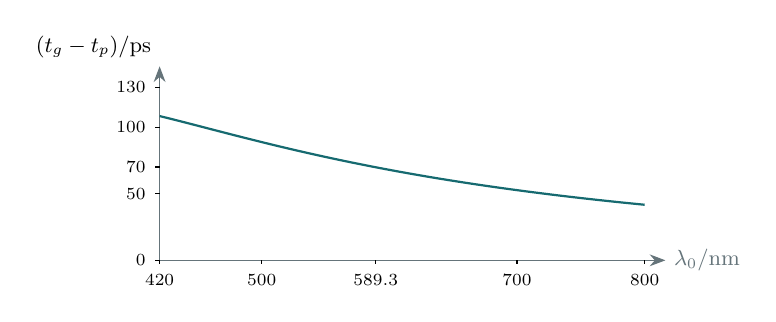
\begin{tikzpicture}[scale=.88,transform shape]
\draw[axis] (0,0.0)--(7.3,0.0) node[right] {$\lambda_0/{\rm nm}$};
\draw[axis] (0,0)--(0,2.8);
\node[above left] at (0,2.8) {$(t_g-t_p)/{\rm ps}$};
\draw[thin] (0.000000,0.0)--(0.000000,-0.06);\node[below,font=\scriptsize] at (0.000000,-0.08) {$ 420 $};
\draw[thin] (1.473684,0.0)--(1.473684,-0.06);\node[below,font=\scriptsize] at (1.473684,-0.08) {$ 500 $};
\draw[thin] (3.118684,0.0)--(3.118684,-0.06);\node[below,font=\scriptsize] at (3.118684,-0.08) {$ 589.3 $};
\draw[thin] (5.157895,0.0)--(5.157895,-0.06);\node[below,font=\scriptsize] at (5.157895,-0.08) {$ 700 $};
\draw[thin] (7.000000,0.0)--(7.000000,-0.06);\node[below,font=\scriptsize] at (7.000000,-0.08) {$ 800 $};
\draw[thin] (0,0.000000)--(-.06,0.000000);\node[left,font=\scriptsize] at (-.08,0.000000) {$ 0 $};
\draw[thin] (0,0.961538)--(-.06,0.961538);\node[left,font=\scriptsize] at (-.08,0.961538) {$ 50 $};
\draw[thin] (0,1.346154)--(-.06,1.346154);\node[left,font=\scriptsize] at (-.08,1.346154) {$ 70 $};
\draw[thin] (0,1.923077)--(-.06,1.923077);\node[left,font=\scriptsize] at (-.08,1.923077) {$ 100 $};
\draw[thin] (0,2.500000)--(-.06,2.500000);\node[left,font=\scriptsize] at (-.08,2.500000) {$ 130 $};
\draw[thick,color=accent] plot coordinates {(0.0000000,2.0818344) (0.0291667,2.0747309) (0.0583333,2.0675806) (0.0875000,2.0603866) (0.1166667,2.0531518) (0.1458333,2.0458790) (0.1750000,2.0385710) (0.2041667,2.0312304) (0.2333333,2.0238596) (0.2625000,2.0164613) (0.2916667,2.0090376) (0.3208333,2.0015908) (0.3500000,1.9941232) (0.3791667,1.9866369) (0.4083333,1.9791339) (0.4375000,1.9716161) (0.4666667,1.9640854) (0.4958333,1.9565436) (0.5250000,1.9489926) (0.5541667,1.9414339) (0.5833333,1.9338692) (0.6125000,1.9263001) (0.6416667,1.9187281) (0.6708333,1.9111545) (0.7000000,1.9035809) (0.7291667,1.8960086) (0.7583333,1.8884388) (0.7875000,1.8808728) (0.8166667,1.8733118) (0.8458333,1.8657570) (0.8750000,1.8582094) (0.9041667,1.8506701) (0.9333333,1.8431402) (0.9625000,1.8356206) (0.9916667,1.8281123) (1.0208333,1.8206161) (1.0500000,1.8131331) (1.0791667,1.8056639) (1.1083333,1.7982094) (1.1375000,1.7907704) (1.1666667,1.7833476) (1.1958333,1.7759417) (1.2250000,1.7685534) (1.2541667,1.7611833) (1.2833333,1.7538322) (1.3125000,1.7465005) (1.3416667,1.7391888) (1.3708333,1.7318977) (1.4000000,1.7246278) (1.4291667,1.7173795) (1.4583333,1.7101532) (1.4875000,1.7029495) (1.5166667,1.6957688) (1.5458333,1.6886115) (1.5750000,1.6814780) (1.6041667,1.6743686) (1.6333333,1.6672838) (1.6625000,1.6602239) (1.6916667,1.6531891) (1.7208333,1.6461798) (1.7500000,1.6391963) (1.7791667,1.6322389) (1.8083333,1.6253078) (1.8375000,1.6184032) (1.8666667,1.6115255) (1.8958333,1.6046747) (1.9250000,1.5978512) (1.9541667,1.5910551) (1.9833333,1.5842866) (2.0125000,1.5775459) (2.0416667,1.5708330) (2.0708333,1.5641482) (2.1000000,1.5574917) (2.1291667,1.5508634) (2.1583333,1.5442636) (2.1875000,1.5376923) (2.2166667,1.5311497) (2.2458333,1.5246358) (2.2750000,1.5181507) (2.3041667,1.5116945) (2.3333333,1.5052672) (2.3625000,1.4988690) (2.3916667,1.4924997) (2.4208333,1.4861596) (2.4500000,1.4798486) (2.4791667,1.4735667) (2.5083333,1.4673139) (2.5375000,1.4610904) (2.5666667,1.4548960) (2.5958333,1.4487308) (2.6250000,1.4425949) (2.6541667,1.4364880) (2.6833333,1.4304104) (2.7125000,1.4243619) (2.7416667,1.4183425) (2.7708333,1.4123521) (2.8000000,1.4063909) (2.8291667,1.4004586) (2.8583333,1.3945554) (2.8875000,1.3886810) (2.9166667,1.3828356) (2.9458333,1.3770190) (2.9750000,1.3712311) (3.0041667,1.3654720) (3.0333333,1.3597415) (3.0625000,1.3540396) (3.0916667,1.3483662) (3.1208333,1.3427213) (3.1500000,1.3371047) (3.1791667,1.3315164) (3.2083333,1.3259563) (3.2375000,1.3204244) (3.2666667,1.3149204) (3.2958333,1.3094445) (3.3250000,1.3039964) (3.3541667,1.2985761) (3.3833333,1.2931834) (3.4125000,1.2878184) (3.4416667,1.2824808) (3.4708333,1.2771706) (3.5000000,1.2718877) (3.5291667,1.2666320) (3.5583333,1.2614034) (3.5875000,1.2562017) (3.6166667,1.2510270) (3.6458333,1.2458790) (3.6750000,1.2407576) (3.7041667,1.2356628) (3.7333333,1.2305945) (3.7625000,1.2255524) (3.7916667,1.2205366) (3.8208333,1.2155469) (3.8500000,1.2105831) (3.8791667,1.2056453) (3.9083333,1.2007331) (3.9375000,1.1958467) (3.9666667,1.1909857) (3.9958333,1.1861501) (4.0250000,1.1813399) (4.0541667,1.1765548) (4.0833333,1.1717947) (4.1125000,1.1670596) (4.1416667,1.1623492) (4.1708333,1.1576636) (4.2000000,1.1530025) (4.2291667,1.1483659) (4.2583333,1.1437535) (4.2875000,1.1391654) (4.3166667,1.1346014) (4.3458333,1.1300613) (4.3750000,1.1255451) (4.4041667,1.1210525) (4.4333333,1.1165836) (4.4625000,1.1121381) (4.4916667,1.1077160) (4.5208333,1.1033171) (4.5500000,1.0989413) (4.5791667,1.0945884) (4.6083333,1.0902585) (4.6375000,1.0859513) (4.6666667,1.0816666) (4.6958333,1.0774045) (4.7250000,1.0731648) (4.7541667,1.0689473) (4.7833333,1.0647519) (4.8125000,1.0605785) (4.8416667,1.0564271) (4.8708333,1.0522973) (4.9000000,1.0481893) (4.9291667,1.0441027) (4.9583333,1.0400376) (4.9875000,1.0359938) (5.0166667,1.0319711) (5.0458333,1.0279695) (5.0750000,1.0239888) (5.1041667,1.0200289) (5.1333333,1.0160897) (5.1625000,1.0121711) (5.1916667,1.0082730) (5.2208333,1.0043952) (5.2500000,1.0005376) (5.2791667,0.9967002) (5.3083333,0.9928827) (5.3375000,0.9890851) (5.3666667,0.9853073) (5.3958333,0.9815492) (5.4250000,0.9778106) (5.4541667,0.9740914) (5.4833333,0.9703915) (5.5125000,0.9667109) (5.5416667,0.9630493) (5.5708333,0.9594067) (5.6000000,0.9557830) (5.6291667,0.9521781) (5.6583333,0.9485918) (5.6875000,0.9450240) (5.7166667,0.9414747) (5.7458333,0.9379437) (5.7750000,0.9344309) (5.8041667,0.9309362) (5.8333333,0.9274595) (5.8625000,0.9240008) (5.8916667,0.9205598) (5.9208333,0.9171365) (5.9500000,0.9137308) (5.9791667,0.9103425) (6.0083333,0.9069716) (6.0375000,0.9036181) (6.0666667,0.9002816) (6.0958333,0.8969623) (6.1250000,0.8936599) (6.1541667,0.8903743) (6.1833333,0.8871056) (6.2125000,0.8838535) (6.2416667,0.8806179) (6.2708333,0.8773988) (6.3000000,0.8741961) (6.3291667,0.8710097) (6.3583333,0.8678394) (6.3875000,0.8646853) (6.4166667,0.8615470) (6.4458333,0.8584247) (6.4750000,0.8553182) (6.5041667,0.8522274) (6.5333333,0.8491521) (6.5625000,0.8460924) (6.5916667,0.8430481) (6.6208333,0.8400191) (6.6500000,0.8370053) (6.6791667,0.8340067) (6.7083333,0.8310232) (6.7375000,0.8280546) (6.7666667,0.8251008) (6.7958333,0.8221619) (6.8250000,0.8192376) (6.8541667,0.8163280) (6.8833333,0.8134328) (6.9125000,0.8105521) (6.9416667,0.8076857) (6.9708333,0.8048336) (7.0000000,0.8019957)};
\end{tikzpicture}
\figcaption{变图光5.1V8\quad 一米样品的群相位时间差测出局部色散}
\end{minipage}\end{center}
\end{enumerate}

\Needspace{13\baselineskip}

\pdfbookmark[2]{第 2 题 氢气的有效共振与振子参数}{q2}

\section*{第 2 题\quad 氢气的有效共振与振子参数}\label{q:2}

常温常压下，氢气在$0.4$至$9\,\mu\mathrm m$波段满足
\[
n^2=1+a+\frac b{\lambda_0^2},\qquad a=2.721\times10^{-4},\quad b=2.11\times10^{-18}\,\mathrm{m^2},
\]
电子吸收带位于远紫外，密度为$9.0\times10^{-2}\,\mathrm{kg/m^3}$。用单振子、弱极化模型估算有效本征频率及共振真空波长；再求振子的荷质比。讨论荷质比的确定需要什么电荷及数密度假设，取氢原子摩尔质量$1.0\times10^{-3}\,\mathrm{kg/mol}$。

\begin{center}\begin{minipage}{.98\linewidth}\centering
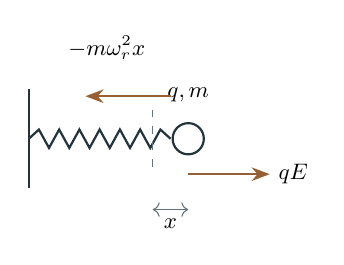
\begin{tikzpicture}[scale=.9,transform shape]
\draw[object] (0.00000,-0.70000)--(0.00000,0.70000);\draw[object] plot coordinates {(0.00000,0.00000) (0.14286,0.13000) (0.28571,-0.13000) (0.42857,0.13000) (0.57143,-0.13000) (0.71429,0.13000) (0.85714,-0.13000) (1.00000,0.13000) (1.14286,-0.13000) (1.28571,0.13000) (1.42857,-0.13000) (1.57143,0.13000) (1.71429,-0.13000) (1.85714,0.13000) (2.00000,0.00000)};\draw[object] (2.25000,0.00000) circle(0.22000);\node[above] at (2.25000,0.40000) {$q,m$};\draw[force] (2.25000,-0.50000)--(3.40000,-0.50000);\node[right] at (3.40000,-0.50000) {$qE$};\draw[force] (2.00000,0.60000)--(0.80000,0.60000);\node[above] at (1.10000,1.00000) {$-m\omega_r^2x$};\draw[<->,thin,color=muted] (1.75000,-1.00000)--(2.25000,-1.00000);\node[below] at (2.00000,-1.00000) {$x$};\draw[guide] (1.75000,-0.40000)--(1.75000,0.40000);
\end{tikzpicture}
\figcaption{图光5.2\quad 束缚振子的外力、回复力与位移。}
\end{minipage}\end{center}

\Needspace{8\baselineskip}

\pdfbookmark[3]{题型定位}{q2-h0}

\subsection*{题型定位}

长波展开的常数与频率平方项共同给有效共振，密度和等效振子计数再给强度。先求$b/a$，后引入$N,e$，可看清共振位置和荷质比各自依赖的条件。

\Needspace{8\baselineskip}

\pdfbookmark[3]{知识点}{q2-h1}

\subsection*{知识点}

\begin{itemize}
\item 受迫振子位移与$qE$成正比，极化再乘$q$，所以线性色散含$q^2/m$。
\item $\omega=2\pi\nu$转换使响应分母带$4\pi^2$，长波展开参数是$(\lambda_r/\lambda_0)^2$。
\item 常数项给$a$，反波长平方项给$b=a\lambda_r^2$，两者比值消去振子强度。
\item 每氢分子两个有效振子与每氢原子一个给相同$N$；电荷大小指定后才从$q^2/m$得到$|q|/m$。
\end{itemize}

\Needspace{8\baselineskip}

\pdfbookmark[3]{物理图像}{q2-h2}

\subsection*{物理图像}

题图的外力、回复力和位移进入同一个受迫方程。解图A标出88nm共振与0.4至9微米窗口，B比较测量区短波端的完整响应和展开，C显示有效计数对荷质比的作用，D以含阻尼示例说明共振处的相位和吸收。模型参数分别在相应观测关系中出现。

\Needspace{8\baselineskip}

\pdfbookmark[3]{解题入口}{q2-h3}

\subsection*{解题入口}

把$1/(\nu_r^2-\nu^2)$提取为$\nu_r^{-2}(1-\nu^2/\nu_r^2)^{-1}$，保留常数和一次平方项。先由$b/a$求$\lambda_r$，再由$a$恢复$Nq^2/m$，最后把题给质量密度转成明确的振子数密度。

\Needspace{8\baselineskip}

\pdfbookmark[3]{标准解法}{q2-h4}

\subsection*{标准解法}


图光5.2中，电荷$q$相对平衡点的位移为$x$，外力为$qE$，回复力为$-m\omega_r^2x$。在远离吸收带的稀薄气体中，用单个有效共振代表该波段的束缚电子响应，先忽略阻尼。取$e^{-i\omega t}$，振动方程及偶极极化为
\[
m\ddot x+m\omega_r^2x=qE,\qquad
x=\frac{qE}{m(\omega_r^2-\omega^2)},\qquad
P=Nqx.
\]
若有多类振子，一般响应为$ n^2-1=(N/\varepsilon_0)\sum_jf_jq_j^2/[m_j(\omega_j^2-\omega^2)]$，$f_j$给各类权重。当前采用一类有效参数，并取局部场近似为宏观场，$P=\varepsilon_0(n^2-1)E$，便得到
\[
n^2-1=\frac{Nq^2}{\varepsilon_0m(\omega_r^2-\omega^2)}
=\frac{Nq^2}{4\pi^2\varepsilon_0m(\nu_r^2-\nu^2)}.
\]
其中$\omega_r=2\pi\nu_r$，从角频率改写成普通频率带来$4\pi^2$因子。令$x_\nu=\nu^2/\nu_r^2=(\lambda_r/\lambda_0)^2$，长波区$0<x_\nu\ll1$有$(1-x_\nu)^{-1}=1+x_\nu+O(x_\nu^2)$，因此
\[
n^2-1\simeq\frac{Nq^2}{4\pi^2\varepsilon_0m\nu_r^2}\left(1+\frac{\nu^2}{\nu_r^2}\right)=\frac{Nq^2}{4\pi^2\varepsilon_0m\nu_r^2}\left(1+\frac{c^2}{\nu_r^2\lambda_0^2}\right).
\]
与题给$n^2-1=a+b/\lambda_0^2$的常数、平方反波长两项分别比较，得
\[
a=\frac{Nq^2}{4\pi^2\varepsilon_0m\nu_r^2},\qquad
b=\frac{ac^2}{\nu_r^2}=a\lambda_r^2.
\]
所以$b/a$直接给共振波长的平方，振子数、电荷与质量在这个比值中消去。解图光5.2A在同一对数波长轴上标出测量窗口与有效共振，二者的距离对应长波展开的尺度。
\begin{center}\begin{minipage}{.98\linewidth}\centering
\begin{tikzpicture}[scale=.9,transform shape]
\draw[axis] (0.00000,0.00000)--(8.50000,0.00000);\node[below right] at (8.50000,0.00000) {$\log\lambda_0$};\draw[force] (0.63863,-0.10000)--(0.63863,1.10000);\node[above] at (0.63863,1.15000) {$\lambda_r=88.06\,\mathrm{nm}$};\draw[very thick,color=accent] (2.34631,0.38000)--(5.85941,0.38000);\draw[<->,thin,color=muted] (2.34631,-0.45000)--(5.85941,-0.45000);\node[below] at (4.10286,-0.45000) {测量波段};\node[above] at (4.00000,1.90000) {长波测量推得的有效共振};
\end{tikzpicture}
\figcaption{解图光5.2A\quad 共振位于测量波段之外；粗线为0.4至9微米。}
\end{minipage}\end{center}
代入$a=2.721\times10^{-4}$、$b=2.11\times10^{-18}\,\mathrm{m^2}$，有
\[
\boxed{\lambda_r=\sqrt{b/a}=8.8060\times10^{-8}\,\mathrm m=88.06\,\mathrm{nm}},
\quad
\boxed{\nu_r=c\sqrt{a/b}=3.407\times10^{15}\,\mathrm{Hz}}.
\]
用未取整的系数得到$\lambda_r=88.05965\,\mathrm{nm}$，按题设精度记约88.1nm。解图光5.2B在测量窗口的短波端比较完整单振子响应$a/(1-x_\nu)$与两项式$a(1+x_\nu)$，显示下一阶项的量级。
\begin{center}\begin{minipage}{.98\linewidth}\centering
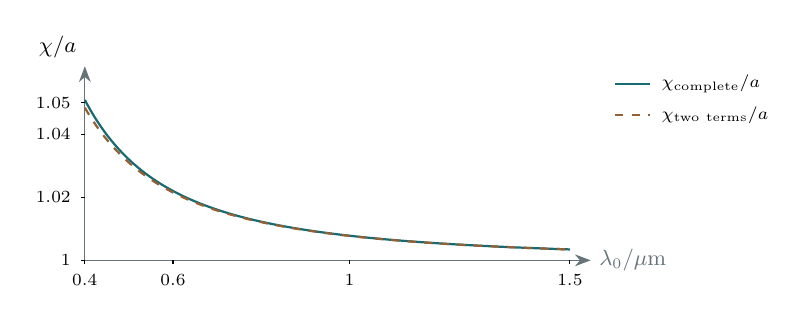
\begin{tikzpicture}[scale=.88,transform shape]
\draw[axis] (0,0)--(7.3,0) node[right] {$\lambda_0/{\rm \mu m}$};
\draw[axis] (0,0)--(0,2.8);
\node[above left] at (0,2.8) {$\chi/a$};
\draw[thin] (0.000000,0)--(0.000000,-0.06);\node[below,font=\scriptsize] at (0.000000,-0.08) {$ 0.4 $};
\draw[thin] (1.272727,0)--(1.272727,-0.06);\node[below,font=\scriptsize] at (1.272727,-0.08) {$ 0.6 $};
\draw[thin] (3.818182,0)--(3.818182,-0.06);\node[below,font=\scriptsize] at (3.818182,-0.08) {$ 1 $};
\draw[thin] (7.000000,0)--(7.000000,-0.06);\node[below,font=\scriptsize] at (7.000000,-0.08) {$ 1.5 $};
\draw[thin] (0,0.000000)--(-.06,0.000000);\node[left,font=\scriptsize] at (-.08,0.000000) {$ 1 $};
\draw[thin] (0,0.909091)--(-.06,0.909091);\node[left,font=\scriptsize] at (-.08,0.909091) {$ 1.02 $};
\draw[thin] (0,1.818182)--(-.06,1.818182);\node[left,font=\scriptsize] at (-.08,1.818182) {$ 1.04 $};
\draw[thin] (0,2.272727)--(-.06,2.272727);\node[left,font=\scriptsize] at (-.08,2.272727) {$ 1.05 $};
\draw[thick,color=accent] plot coordinates {(0.0000000,2.3151907) (0.0291667,2.2604386) (0.0583333,2.2076353) (0.0875000,2.1566881) (0.1166667,2.1075097) (0.1458333,2.0600182) (0.1750000,2.0141363) (0.2041667,1.9697910) (0.2333333,1.9269137) (0.2625000,1.8854395) (0.2916667,1.8453070) (0.3208333,1.8064583) (0.3500000,1.7688387) (0.3791667,1.7323961) (0.4083333,1.6970815) (0.4375000,1.6628482) (0.4666667,1.6296521) (0.4958333,1.5974513) (0.5250000,1.5662059) (0.5541667,1.5358781) (0.5833333,1.5064319) (0.6125000,1.4778333) (0.6416667,1.4500496) (0.6708333,1.4230499) (0.7000000,1.3968046) (0.7291667,1.3712858) (0.7583333,1.3464665) (0.7875000,1.3223212) (0.8166667,1.2988255) (0.8458333,1.2759562) (0.8750000,1.2536908) (0.9041667,1.2320083) (0.9333333,1.2108882) (0.9625000,1.1903111) (0.9916667,1.1702584) (1.0208333,1.1507123) (1.0500000,1.1316557) (1.0791667,1.1130723) (1.1083333,1.0949465) (1.1375000,1.0772632) (1.1666667,1.0600081) (1.1958333,1.0431673) (1.2250000,1.0267276) (1.2541667,1.0106762) (1.2833333,0.9950009) (1.3125000,0.9796901) (1.3416667,0.9647323) (1.3708333,0.9501169) (1.4000000,0.9358332) (1.4291667,0.9218714) (1.4583333,0.9082217) (1.4875000,0.8948748) (1.5166667,0.8818218) (1.5458333,0.8690542) (1.5750000,0.8565635) (1.6041667,0.8443418) (1.6333333,0.8323813) (1.6625000,0.8206747) (1.6916667,0.8092147) (1.7208333,0.7979945) (1.7500000,0.7870073) (1.7791667,0.7762468) (1.8083333,0.7657066) (1.8375000,0.7553808) (1.8666667,0.7452636) (1.8958333,0.7353494) (1.9250000,0.7256327) (1.9541667,0.7161083) (1.9833333,0.7067712) (2.0125000,0.6976164) (2.0416667,0.6886392) (2.0708333,0.6798350) (2.1000000,0.6711994) (2.1291667,0.6627281) (2.1583333,0.6544169) (2.1875000,0.6462618) (2.2166667,0.6382589) (2.2458333,0.6304044) (2.2750000,0.6226946) (2.3041667,0.6151260) (2.3333333,0.6076952) (2.3625000,0.6003988) (2.3916667,0.5932336) (2.4208333,0.5861964) (2.4500000,0.5792842) (2.4791667,0.5724941) (2.5083333,0.5658231) (2.5375000,0.5592686) (2.5666667,0.5528277) (2.5958333,0.5464979) (2.6250000,0.5402765) (2.6541667,0.5341613) (2.6833333,0.5281497) (2.7125000,0.5222393) (2.7416667,0.5164280) (2.7708333,0.5107135) (2.8000000,0.5050937) (2.8291667,0.4995665) (2.8583333,0.4941298) (2.8875000,0.4887817) (2.9166667,0.4835202) (2.9458333,0.4783436) (2.9750000,0.4732499) (3.0041667,0.4682374) (3.0333333,0.4633044) (3.0625000,0.4584493) (3.0916667,0.4536702) (3.1208333,0.4489658) (3.1500000,0.4443344) (3.1791667,0.4397745) (3.2083333,0.4352847) (3.2375000,0.4308635) (3.2666667,0.4265095) (3.2958333,0.4222214) (3.3250000,0.4179978) (3.3541667,0.4138375) (3.3833333,0.4097391) (3.4125000,0.4057015) (3.4416667,0.4017235) (3.4708333,0.3978039) (3.5000000,0.3939415) (3.5291667,0.3901352) (3.5583333,0.3863840) (3.5875000,0.3826868) (3.6166667,0.3790426) (3.6458333,0.3754503) (3.6750000,0.3719090) (3.7041667,0.3684176) (3.7333333,0.3649754) (3.7625000,0.3615812) (3.7916667,0.3582344) (3.8208333,0.3549339) (3.8500000,0.3516789) (3.8791667,0.3484686) (3.9083333,0.3453021) (3.9375000,0.3421788) (3.9666667,0.3390977) (3.9958333,0.3360582) (4.0250000,0.3330594) (4.0541667,0.3301007) (4.0833333,0.3271814) (4.1125000,0.3243006) (4.1416667,0.3214579) (4.1708333,0.3186525) (4.2000000,0.3158837) (4.2291667,0.3131509) (4.2583333,0.3104535) (4.2875000,0.3077909) (4.3166667,0.3051625) (4.3458333,0.3025676) (4.3750000,0.3000058) (4.4041667,0.2974765) (4.4333333,0.2949791) (4.4625000,0.2925130) (4.4916667,0.2900779) (4.5208333,0.2876731) (4.5500000,0.2852981) (4.5791667,0.2829525) (4.6083333,0.2806357) (4.6375000,0.2783473) (4.6666667,0.2760869) (4.6958333,0.2738539) (4.7250000,0.2716480) (4.7541667,0.2694687) (4.7833333,0.2673155) (4.8125000,0.2651881) (4.8416667,0.2630861) (4.8708333,0.2610090) (4.9000000,0.2589564) (4.9291667,0.2569280) (4.9583333,0.2549234) (4.9875000,0.2529422) (5.0166667,0.2509840) (5.0458333,0.2490486) (5.0750000,0.2471354) (5.1041667,0.2452443) (5.1333333,0.2433749) (5.1625000,0.2415267) (5.1916667,0.2396996) (5.2208333,0.2378932) (5.2500000,0.2361071) (5.2791667,0.2343411) (5.3083333,0.2325949) (5.3375000,0.2308682) (5.3666667,0.2291607) (5.3958333,0.2274720) (5.4250000,0.2258020) (5.4541667,0.2241504) (5.4833333,0.2225168) (5.5125000,0.2209011) (5.5416667,0.2193029) (5.5708333,0.2177220) (5.6000000,0.2161582) (5.6291667,0.2146112) (5.6583333,0.2130807) (5.6875000,0.2115667) (5.7166667,0.2100687) (5.7458333,0.2085866) (5.7750000,0.2071201) (5.8041667,0.2056691) (5.8333333,0.2042333) (5.8625000,0.2028125) (5.8916667,0.2014065) (5.9208333,0.2000151) (5.9500000,0.1986381) (5.9791667,0.1972752) (6.0083333,0.1959264) (6.0375000,0.1945914) (6.0666667,0.1932700) (6.0958333,0.1919620) (6.1250000,0.1906673) (6.1541667,0.1893856) (6.1833333,0.1881169) (6.2125000,0.1868608) (6.2416667,0.1856174) (6.2708333,0.1843863) (6.3000000,0.1831674) (6.3291667,0.1819606) (6.3583333,0.1807657) (6.3875000,0.1795825) (6.4166667,0.1784110) (6.4458333,0.1772509) (6.4750000,0.1761020) (6.5041667,0.1749644) (6.5333333,0.1738377) (6.5625000,0.1727219) (6.5916667,0.1716168) (6.6208333,0.1705223) (6.6500000,0.1694382) (6.6791667,0.1683645) (6.7083333,0.1673009) (6.7375000,0.1662475) (6.7666667,0.1652039) (6.7958333,0.1641701) (6.8250000,0.1631461) (6.8541667,0.1621316) (6.8833333,0.1611265) (6.9125000,0.1601308) (6.9416667,0.1591442) (6.9708333,0.1581668) (7.0000000,0.1571984)};
\draw[thick,color=accent] (7.65,2.55)--(8.15,2.55);\node[right,font=\scriptsize] at (8.2,2.55) {$\chi_{\rm complete}/a$};
\draw[thick,dashed,color=warm] plot coordinates {(0.0000000,2.2029835) (0.0291667,2.1533531) (0.0583333,2.1053812) (0.0875000,2.0589947) (0.1166667,2.0141244) (0.1458333,1.9707051) (0.1750000,1.9286747) (0.2041667,1.8879748) (0.2333333,1.8485498) (0.2625000,1.8103469) (0.2916667,1.7733161) (0.3208333,1.7374100) (0.3500000,1.7025836) (0.3791667,1.6687939) (0.4083333,1.6360001) (0.4375000,1.6041637) (0.4666667,1.5732475) (0.4958333,1.5432166) (0.5250000,1.5140374) (0.5541667,1.4856780) (0.5833333,1.4581080) (0.6125000,1.4312984) (0.6416667,1.4052215) (0.6708333,1.3798508) (0.7000000,1.3551610) (0.7291667,1.3311279) (0.7583333,1.3077286) (0.7875000,1.2849409) (0.8166667,1.2627437) (0.8458333,1.2411167) (0.8750000,1.2200406) (0.9041667,1.1994969) (0.9333333,1.1794677) (0.9625000,1.1599360) (0.9916667,1.1408855) (1.0208333,1.1223005) (1.0500000,1.1041659) (1.0791667,1.0864674) (1.1083333,1.0691910) (1.1375000,1.0523234) (1.1666667,1.0358518) (1.1958333,1.0197640) (1.2250000,1.0040481) (1.2541667,0.9886927) (1.2833333,0.9736869) (1.3125000,0.9590201) (1.3416667,0.9446823) (1.3708333,0.9306636) (1.4000000,0.9169546) (1.4291667,0.9035464) (1.4583333,0.8904301) (1.4875000,0.8775973) (1.5166667,0.8650400) (1.5458333,0.8527503) (1.5750000,0.8407206) (1.6041667,0.8289437) (1.6333333,0.8174125) (1.6625000,0.8061203) (1.6916667,0.7950605) (1.7208333,0.7842267) (1.7500000,0.7736129) (1.7791667,0.7632131) (1.8083333,0.7530216) (1.8375000,0.7430328) (1.8666667,0.7332416) (1.8958333,0.7236425) (1.9250000,0.7142308) (1.9541667,0.7050015) (1.9833333,0.6959499) (2.0125000,0.6870715) (2.0416667,0.6783620) (2.0708333,0.6698170) (2.1000000,0.6614325) (2.1291667,0.6532044) (2.1583333,0.6451289) (2.1875000,0.6372022) (2.2166667,0.6294207) (2.2458333,0.6217809) (2.2750000,0.6142794) (2.3041667,0.6069128) (2.3333333,0.5996779) (2.3625000,0.5925717) (2.3916667,0.5855910) (2.4208333,0.5787329) (2.4500000,0.5719946) (2.4791667,0.5653733) (2.5083333,0.5588663) (2.5375000,0.5524710) (2.5666667,0.5461849) (2.5958333,0.5400054) (2.6250000,0.5339302) (2.6541667,0.5279570) (2.6833333,0.5220834) (2.7125000,0.5163073) (2.7416667,0.5106266) (2.7708333,0.5050391) (2.8000000,0.4995428) (2.8291667,0.4941357) (2.8583333,0.4888159) (2.8875000,0.4835816) (2.9166667,0.4784310) (2.9458333,0.4733621) (2.9750000,0.4683734) (3.0041667,0.4634632) (3.0333333,0.4586298) (3.0625000,0.4538716) (3.0916667,0.4491870) (3.1208333,0.4445746) (3.1500000,0.4400329) (3.1791667,0.4355604) (3.2083333,0.4311558) (3.2375000,0.4268177) (3.2666667,0.4225447) (3.2958333,0.4183355) (3.3250000,0.4141889) (3.3541667,0.4101037) (3.3833333,0.4060786) (3.4125000,0.4021125) (3.4416667,0.3982042) (3.4708333,0.3943526) (3.5000000,0.3905566) (3.5291667,0.3868152) (3.5583333,0.3831273) (3.5875000,0.3794918) (3.6166667,0.3759079) (3.6458333,0.3723745) (3.6750000,0.3688907) (3.7041667,0.3654555) (3.7333333,0.3620681) (3.7625000,0.3587276) (3.7916667,0.3554331) (3.8208333,0.3521838) (3.8500000,0.3489789) (3.8791667,0.3458174) (3.9083333,0.3426988) (3.9375000,0.3396221) (3.9666667,0.3365867) (3.9958333,0.3335918) (4.0250000,0.3306367) (4.0541667,0.3277207) (4.0833333,0.3248431) (4.1125000,0.3220033) (4.1416667,0.3192005) (4.1708333,0.3164341) (4.2000000,0.3137036) (4.2291667,0.3110082) (4.2583333,0.3083475) (4.2875000,0.3057207) (4.3166667,0.3031274) (4.3458333,0.3005669) (4.3750000,0.2980387) (4.4041667,0.2955423) (4.4333333,0.2930771) (4.4625000,0.2906427) (4.4916667,0.2882384) (4.5208333,0.2858639) (4.5500000,0.2835186) (4.5791667,0.2812020) (4.6083333,0.2789137) (4.6375000,0.2766532) (4.6666667,0.2744201) (4.6958333,0.2722139) (4.7250000,0.2700342) (4.7541667,0.2678806) (4.7833333,0.2657527) (4.8125000,0.2636500) (4.8416667,0.2615721) (4.8708333,0.2595188) (4.9000000,0.2574895) (4.9291667,0.2554839) (4.9583333,0.2535017) (4.9875000,0.2515424) (5.0166667,0.2496058) (5.0458333,0.2476915) (5.0750000,0.2457990) (5.1041667,0.2439282) (5.1333333,0.2420787) (5.1625000,0.2402501) (5.1916667,0.2384422) (5.2208333,0.2366546) (5.2500000,0.2348870) (5.2791667,0.2331392) (5.3083333,0.2314108) (5.3375000,0.2297015) (5.3666667,0.2280111) (5.3958333,0.2263393) (5.4250000,0.2246859) (5.4541667,0.2230504) (5.4833333,0.2214328) (5.5125000,0.2198327) (5.5416667,0.2182499) (5.5708333,0.2166841) (5.6000000,0.2151351) (5.6291667,0.2136027) (5.6583333,0.2120865) (5.6875000,0.2105865) (5.7166667,0.2091023) (5.7458333,0.2076338) (5.7750000,0.2061806) (5.8041667,0.2047427) (5.8333333,0.2033197) (5.8625000,0.2019116) (5.8916667,0.2005180) (5.9208333,0.1991388) (5.9500000,0.1977738) (5.9791667,0.1964227) (6.0083333,0.1950855) (6.0375000,0.1937619) (6.0666667,0.1924517) (6.0958333,0.1911547) (6.1250000,0.1898708) (6.1541667,0.1885998) (6.1833333,0.1873415) (6.2125000,0.1860958) (6.2416667,0.1848625) (6.2708333,0.1836413) (6.3000000,0.1824323) (6.3291667,0.1812351) (6.3583333,0.1800497) (6.3875000,0.1788758) (6.4166667,0.1777135) (6.4458333,0.1765624) (6.4750000,0.1754224) (6.5041667,0.1742935) (6.5333333,0.1731754) (6.5625000,0.1720680) (6.5916667,0.1709713) (6.6208333,0.1698850) (6.6500000,0.1688090) (6.6791667,0.1677432) (6.7083333,0.1666874) (6.7375000,0.1656416) (6.7666667,0.1646056) (6.7958333,0.1635793) (6.8250000,0.1625626) (6.8541667,0.1615553) (6.8833333,0.1605574) (6.9125000,0.1595686) (6.9416667,0.1585890) (6.9708333,0.1576184) (7.0000000,0.1566566)};
\draw[thick,dashed,color=warm] (7.65,2.0999999999999996)--(8.15,2.0999999999999996);\node[right,font=\scriptsize] at (8.2,2.0999999999999996) {$\chi_{\rm two\ terms}/a$};
\end{tikzpicture}
\figcaption{解图光5.2B\quad 测量窗口短波端的完整单振子响应与两项展开}
\end{minipage}\end{center}
再由$a$的定义消去$\nu_r^2=c^2a/b$，保留光学数据直接约束的量：
\[
\boxed{\frac{q^2}{m}=\frac{4\pi^2\varepsilon_0c^2a^2}{Nb}}.
\]
为了把质量密度换成该式的$N$，采用每氢原子一个有效电子振子，即每氢分子两个。常温常压的分子数密度为$\rho N_A/(2M_{\rm H})$，乘2后得到
\[
N=\frac{\rho N_A}{M_{\mathrm H}}\simeq5.42\times10^{25}\,\mathrm{m^{-3}}.
\]
这里$M_{\rm H}=1.0\times10^{-3}\,\mathrm{kg/mol}$。若再指定电荷大小$|q|=e$，才把$q^2/m$换成荷质比：
\[
\boxed{\frac{|q|}{m}=\frac{4\pi^2\varepsilon_0c^2a^2}{Neb}
\simeq1.27\times10^{11}\,\mathrm{C/kg}}.
\]
为说明有效参数的数值，取$N_A=6.02214\times10^{23}\,\mathrm{mol^{-1}}$、$\varepsilon_0=8.85419\times10^{-12}\,\mathrm{F/m}$、$e=1.60218\times10^{-19}\,\mathrm C$，得$N=5.419926\times10^{25}\,\mathrm{m^{-3}}$、$q^2/m=2.036725\times10^{-8}\,\mathrm{C^2/kg}$及$|q|/m=1.271221\times10^{11}\,\mathrm{C/kg}$。解图光5.2C把改变等效振子计数时的荷质比画出：相同光学系数下，推得$q^2/m$与采用的$N$成反比。
\begin{center}\begin{minipage}{.98\linewidth}\centering
\begin{tikzpicture}[scale=.88,transform shape]
\draw[axis] (0,0)--(7.3,0) node[right] {$N^\prime/N$};
\draw[axis] (0,0)--(0,2.8);
\node[above left] at (0,2.8) {$(|q|/m)/(10^{11}{\rm C/kg})$};
\draw[thin] (0.000000,0)--(0.000000,-0.06);\node[below,font=\scriptsize] at (0.000000,-0.08) {$ 0.5 $};
\draw[thin] (2.333333,0)--(2.333333,-0.06);\node[below,font=\scriptsize] at (2.333333,-0.08) {$ 1 $};
\draw[thin] (4.666667,0)--(4.666667,-0.06);\node[below,font=\scriptsize] at (4.666667,-0.08) {$ 1.5 $};
\draw[thin] (7.000000,0)--(7.000000,-0.06);\node[below,font=\scriptsize] at (7.000000,-0.08) {$ 2 $};
\draw[thin] (0,0.000000)--(-.06,0.000000);\node[left,font=\scriptsize] at (-.08,0.000000) {$ 0.6 $};
\draw[thin] (0,0.837500)--(-.06,0.837500);\node[left,font=\scriptsize] at (-.08,0.837500) {$ 1.27 $};
\draw[thin] (0,1.750000)--(-.06,1.750000);\node[left,font=\scriptsize] at (-.08,1.750000) {$ 2 $};
\draw[thin] (0,2.500000)--(-.06,2.500000);\node[left,font=\scriptsize] at (-.08,2.500000) {$ 2.6 $};
\draw[thick,color=accent] plot coordinates {(0.0000000,2.4280524) (0.0291667,2.3888172) (0.0583333,2.3505390) (0.0875000,2.3131831) (0.1166667,2.2767166) (0.1458333,2.2411082) (0.1750000,2.2063278) (0.2041667,2.1723471) (0.2333333,2.1391386) (0.2625000,2.1066763) (0.2916667,2.0749355) (0.3208333,2.0438922) (0.3500000,2.0135238) (0.3791667,1.9838085) (0.4083333,1.9547255) (0.4375000,1.9262547) (0.4666667,1.8983770) (0.4958333,1.8710742) (0.5250000,1.8443285) (0.5541667,1.8181232) (0.5833333,1.7924419) (0.6125000,1.7672692) (0.6416667,1.7425901) (0.6708333,1.7183902) (0.7000000,1.6946557) (0.7291667,1.6713733) (0.7583333,1.6485301) (0.7875000,1.6261140) (0.8166667,1.6041129) (0.8458333,1.5825155) (0.8750000,1.5613109) (0.9041667,1.5404882) (0.9333333,1.5200374) (0.9625000,1.4999486) (0.9916667,1.4802122) (1.0208333,1.4608191) (1.0500000,1.4417603) (1.0791667,1.4230273) (1.1083333,1.4046118) (1.1375000,1.3865058) (1.1666667,1.3687016) (1.1958333,1.3511917) (1.2250000,1.3339688) (1.2541667,1.3170260) (1.2833333,1.3003564) (1.3125000,1.2839536) (1.3416667,1.2678111) (1.3708333,1.2519228) (1.4000000,1.2362828) (1.4291667,1.2208852) (1.4583333,1.2057246) (1.4875000,1.1907954) (1.5166667,1.1760924) (1.5458333,1.1616105) (1.5750000,1.1473447) (1.6041667,1.1332903) (1.6333333,1.1194426) (1.6625000,1.1057970) (1.6916667,1.0923492) (1.7208333,1.0790949) (1.7500000,1.0660300) (1.7791667,1.0531503) (1.8083333,1.0404521) (1.8375000,1.0279314) (1.8666667,1.0155847) (1.8958333,1.0034082) (1.9250000,0.9913986) (1.9541667,0.9795523) (1.9833333,0.9678662) (2.0125000,0.9563369) (2.0416667,0.9449613) (2.0708333,0.9337364) (2.1000000,0.9226592) (2.1291667,0.9117268) (2.1583333,0.9009363) (2.1875000,0.8902851) (2.2166667,0.8797705) (2.2458333,0.8693898) (2.2750000,0.8591405) (2.3041667,0.8490201) (2.3333333,0.8390262) (2.3625000,0.8291565) (2.3916667,0.8194086) (2.4208333,0.8097803) (2.4500000,0.8002695) (2.4791667,0.7908739) (2.5083333,0.7815915) (2.5375000,0.7724203) (2.5666667,0.7633583) (2.5958333,0.7544035) (2.6250000,0.7455541) (2.6541667,0.7368082) (2.6833333,0.7281639) (2.7125000,0.7196196) (2.7416667,0.7111735) (2.7708333,0.7028240) (2.8000000,0.6945693) (2.8291667,0.6864079) (2.8583333,0.6783382) (2.8875000,0.6703586) (2.9166667,0.6624677) (2.9458333,0.6546641) (2.9750000,0.6469461) (3.0041667,0.6393125) (3.0333333,0.6317619) (3.0625000,0.6242929) (3.0916667,0.6169043) (3.1208333,0.6095946) (3.1500000,0.6023627) (3.1791667,0.5952074) (3.2083333,0.5881273) (3.2375000,0.5811214) (3.2666667,0.5741885) (3.2958333,0.5673274) (3.3250000,0.5605371) (3.3541667,0.5538164) (3.3833333,0.5471643) (3.4125000,0.5405797) (3.4416667,0.5340616) (3.4708333,0.5276090) (3.5000000,0.5212210) (3.5291667,0.5148965) (3.5583333,0.5086346) (3.5875000,0.5024345) (3.6166667,0.4962951) (3.6458333,0.4902156) (3.6750000,0.4841951) (3.7041667,0.4782328) (3.7333333,0.4723279) (3.7625000,0.4664794) (3.7916667,0.4606866) (3.8208333,0.4549488) (3.8500000,0.4492651) (3.8791667,0.4436347) (3.9083333,0.4380570) (3.9375000,0.4325311) (3.9666667,0.4270565) (3.9958333,0.4216322) (4.0250000,0.4162578) (4.0541667,0.4109324) (4.0833333,0.4056554) (4.1125000,0.4004262) (4.1416667,0.3952441) (4.1708333,0.3901085) (4.2000000,0.3850187) (4.2291667,0.3799742) (4.2583333,0.3749743) (4.2875000,0.3700185) (4.3166667,0.3651061) (4.3458333,0.3602367) (4.3750000,0.3554095) (4.4041667,0.3506242) (4.4333333,0.3458801) (4.4625000,0.3411768) (4.4916667,0.3365136) (4.5208333,0.3318902) (4.5500000,0.3273059) (4.5791667,0.3227603) (4.6083333,0.3182529) (4.6375000,0.3137832) (4.6666667,0.3093508) (4.6958333,0.3049552) (4.7250000,0.3005958) (4.7541667,0.2962724) (4.7833333,0.2919844) (4.8125000,0.2877314) (4.8416667,0.2835130) (4.8708333,0.2793287) (4.9000000,0.2751782) (4.9291667,0.2710610) (4.9583333,0.2669768) (4.9875000,0.2629251) (5.0166667,0.2589055) (5.0458333,0.2549178) (5.0750000,0.2509614) (5.1041667,0.2470361) (5.1333333,0.2431414) (5.1625000,0.2392770) (5.1916667,0.2354426) (5.2208333,0.2316378) (5.2500000,0.2278623) (5.2791667,0.2241157) (5.3083333,0.2203977) (5.3375000,0.2167080) (5.3666667,0.2130462) (5.3958333,0.2094121) (5.4250000,0.2058052) (5.4541667,0.2022254) (5.4833333,0.1986724) (5.5125000,0.1951457) (5.5416667,0.1916452) (5.5708333,0.1881705) (5.6000000,0.1847213) (5.6291667,0.1812974) (5.6583333,0.1778985) (5.6875000,0.1745243) (5.7166667,0.1711746) (5.7458333,0.1678491) (5.7750000,0.1645475) (5.8041667,0.1612695) (5.8333333,0.1580150) (5.8625000,0.1547836) (5.8916667,0.1515752) (5.9208333,0.1483894) (5.9500000,0.1452260) (5.9791667,0.1420849) (6.0083333,0.1389657) (6.0375000,0.1358683) (6.0666667,0.1327923) (6.0958333,0.1297377) (6.1250000,0.1267041) (6.1541667,0.1236914) (6.1833333,0.1206993) (6.2125000,0.1177276) (6.2416667,0.1147762) (6.2708333,0.1118447) (6.3000000,0.1089331) (6.3291667,0.1060411) (6.3583333,0.1031684) (6.3875000,0.1003150) (6.4166667,0.0974806) (6.4458333,0.0946651) (6.4750000,0.0918682) (6.5041667,0.0890897) (6.5333333,0.0863296) (6.5625000,0.0835875) (6.5916667,0.0808634) (6.6208333,0.0781570) (6.6500000,0.0754682) (6.6791667,0.0727967) (6.7083333,0.0701426) (6.7375000,0.0675054) (6.7666667,0.0648852) (6.7958333,0.0622818) (6.8250000,0.0596949) (6.8541667,0.0571244) (6.8833333,0.0545702) (6.9125000,0.0520322) (6.9416667,0.0495100) (6.9708333,0.0470037) (7.0000000,0.0445131)};
\end{tikzpicture}
\figcaption{解图光5.2C\quad 固定光学系数和电荷大小时计数改变所推荷质比}
\end{minipage}\end{center}
折射率响应含$q^2$，电荷正负不进入上述色散。若写$|q|=ke$，数据约束的是$k^2e/m$；取单电子电荷$k=1$是当前有效电子振子的模型条件。用$m_e=9.10938\times10^{-31}\,\mathrm{kg}$比较，电子荷质比约$1.75882\times10^{11}\,\mathrm{C/kg}$，本估计低约27.7\%。固定真实电子质量和电荷时，可把同一差异写成有效强度$f=(q^2/m)_{\rm eff}/(e^2/m_e)=.72277\simeq.723$。这组长波数据把多个电子跃迁和分子响应合并为有效共振、有效强度，给出了相应近似下的质量或权重。

在最短测量波长400nm处，$x_\nu=.0484656$。下一项相对静态项为$x_\nu^2=.00234892$，全部高阶尾项相对静态项为$x_\nu^2/(1-x_\nu)=.00246856$；两项式相对完整单振子响应的误差恰为$x_\nu^2$。这一展开由测量窗口的长波条件控制，88nm处的共振局部响应改用含阻尼的完整方程。

例如令$\gamma=.05\omega_r$，阻尼方程给
\[
 m\ddot x+m\gamma\dot x+m\omega_r^2x=qE,\qquad
 \frac{n^2-1}{a}=\frac1{1-u^2-i\Gamma u},\quad
 u=\omega/\omega_r,\quad\Gamma=\gamma/\omega_r.
\]
解图光5.2D用这组示例参数展示共振附近的实、虚响应，虚部为正，对应被动吸收。峰宽由阻尼控制；单纯的两个实长波系数给共振尺度和有效强度，损耗谱再提供阻尼信息。
\begin{center}\begin{minipage}{.98\linewidth}\centering
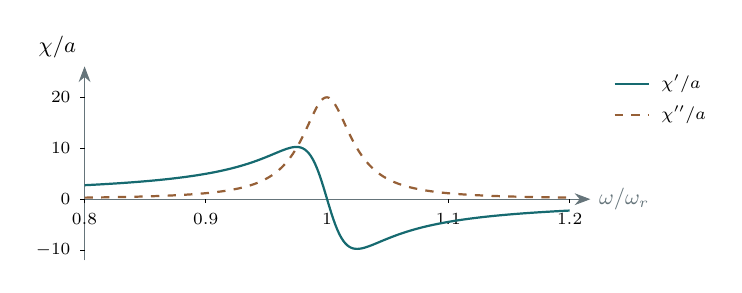
\begin{tikzpicture}[scale=.88,transform shape]
\draw[axis] (0,0.8823529411764706)--(7.3,0.8823529411764706) node[right] {$\omega/\omega_r$};
\draw[axis] (0,0)--(0,2.8);
\node[above left] at (0,2.8) {$\chi/a$};
\draw[thin] (0.000000,0.8823529411764706)--(0.000000,0.8223529411764705);\node[below,font=\scriptsize] at (0.000000,0.8023529411764706) {$ 0.8 $};
\draw[thin] (1.750000,0.8823529411764706)--(1.750000,0.8223529411764705);\node[below,font=\scriptsize] at (1.750000,0.8023529411764706) {$ 0.9 $};
\draw[thin] (3.500000,0.8823529411764706)--(3.500000,0.8223529411764705);\node[below,font=\scriptsize] at (3.500000,0.8023529411764706) {$ 1 $};
\draw[thin] (5.250000,0.8823529411764706)--(5.250000,0.8223529411764705);\node[below,font=\scriptsize] at (5.250000,0.8023529411764706) {$ 1.1 $};
\draw[thin] (7.000000,0.8823529411764706)--(7.000000,0.8223529411764705);\node[below,font=\scriptsize] at (7.000000,0.8023529411764706) {$ 1.2 $};
\draw[thin] (0,0.147059)--(-.06,0.147059);\node[left,font=\scriptsize] at (-.08,0.147059) {$ -10 $};
\draw[thin] (0,0.882353)--(-.06,0.882353);\node[left,font=\scriptsize] at (-.08,0.882353) {$ 0 $};
\draw[thin] (0,1.617647)--(-.06,1.617647);\node[left,font=\scriptsize] at (-.08,1.617647) {$ 10 $};
\draw[thin] (0,2.352941)--(-.06,2.352941);\node[left,font=\scriptsize] at (-.08,2.352941) {$ 20 $};
\draw[thick,color=accent] plot coordinates {(0.0000000,1.0841105) (0.0291667,1.0855700) (0.0583333,1.0870536) (0.0875000,1.0885616) (0.1166667,1.0900947) (0.1458333,1.0916535) (0.1750000,1.0932386) (0.2041667,1.0948507) (0.2333333,1.0964905) (0.2625000,1.0981586) (0.2916667,1.0998558) (0.3208333,1.1015828) (0.3500000,1.1033403) (0.3791667,1.1051292) (0.4083333,1.1069503) (0.4375000,1.1088044) (0.4666667,1.1106923) (0.4958333,1.1126151) (0.5250000,1.1145736) (0.5541667,1.1165687) (0.5833333,1.1186016) (0.6125000,1.1206732) (0.6416667,1.1227846) (0.6708333,1.1249369) (0.7000000,1.1271313) (0.7291667,1.1293689) (0.7583333,1.1316510) (0.7875000,1.1339790) (0.8166667,1.1363540) (0.8458333,1.1387776) (0.8750000,1.1412511) (0.9041667,1.1437760) (0.9333333,1.1463540) (0.9625000,1.1489865) (0.9916667,1.1516753) (1.0208333,1.1544220) (1.0500000,1.1572286) (1.0791667,1.1600969) (1.1083333,1.1630288) (1.1375000,1.1660263) (1.1666667,1.1690916) (1.1958333,1.1722269) (1.2250000,1.1754344) (1.2541667,1.1787166) (1.2833333,1.1820759) (1.3125000,1.1855149) (1.3416667,1.1890363) (1.3708333,1.1926429) (1.4000000,1.1963376) (1.4291667,1.2001234) (1.4583333,1.2040036) (1.4875000,1.2079814) (1.5166667,1.2120603) (1.5458333,1.2162438) (1.5750000,1.2205358) (1.6041667,1.2249401) (1.6333333,1.2294607) (1.6625000,1.2341020) (1.6916667,1.2388683) (1.7208333,1.2437643) (1.7500000,1.2487946) (1.7791667,1.2539643) (1.8083333,1.2592787) (1.8375000,1.2647429) (1.8666667,1.2703627) (1.8958333,1.2761439) (1.9250000,1.2820924) (1.9541667,1.2882145) (1.9833333,1.2945165) (2.0125000,1.3010052) (2.0416667,1.3076872) (2.0708333,1.3145697) (2.1000000,1.3216596) (2.1291667,1.3289643) (2.1583333,1.3364910) (2.1875000,1.3442472) (2.2166667,1.3522401) (2.2458333,1.3604770) (2.2750000,1.3689649) (2.3041667,1.3777106) (2.3333333,1.3867203) (2.3625000,1.3959995) (2.3916667,1.4055531) (2.4208333,1.4153845) (2.4500000,1.4254958) (2.4791667,1.4358872) (2.5083333,1.4465565) (2.5375000,1.4574982) (2.5666667,1.4687033) (2.5958333,1.4801578) (2.6250000,1.4918422) (2.6541667,1.5037295) (2.6833333,1.5157838) (2.7125000,1.5279585) (2.7416667,1.5401937) (2.7708333,1.5524132) (2.8000000,1.5645214) (2.8291667,1.5763990) (2.8583333,1.5878980) (2.8875000,1.5988364) (2.9166667,1.6089917) (2.9458333,1.6180937) (2.9750000,1.6258164) (3.0041667,1.6317697) (3.0333333,1.6354914) (3.0625000,1.6364396) (3.0916667,1.6339874) (3.1208333,1.6274221) (3.1500000,1.6159502) (3.1791667,1.5987126) (3.2083333,1.5748128) (3.2375000,1.5433624) (3.2666667,1.5035458) (3.2958333,1.4547055) (3.3250000,1.3964435) (3.3541667,1.3287301) (3.3833333,1.2520035) (3.4125000,1.1672385) (3.4416667,1.0759627) (3.4708333,0.9802022) (3.5000000,0.8823529) (3.5291667,0.7849903) (3.5583333,0.6906473) (3.5875000,0.6016008) (3.6166667,0.5197011) (3.6458333,0.4462709) (3.6750000,0.3820784) (3.7041667,0.3273760) (3.7333333,0.2819834) (3.7625000,0.2453927) (3.7916667,0.2168759) (3.8208333,0.1955811) (3.8500000,0.1806105) (3.8791667,0.1710771) (3.9083333,0.1661440) (3.9375000,0.1650468) (3.9666667,0.1671049) (3.9958333,0.1717235) (4.0250000,0.1783915) (4.0541667,0.1866745) (4.0833333,0.1962076) (4.1125000,0.2066866) (4.1416667,0.2178601) (4.1708333,0.2295216) (4.2000000,0.2415026) (4.2291667,0.2536664) (4.2583333,0.2659033) (4.2875000,0.2781251) (4.3166667,0.2902623) (4.3458333,0.3022603) (4.3750000,0.3140766) (4.4041667,0.3256791) (4.4333333,0.3370437) (4.4625000,0.3481530) (4.4916667,0.3589951) (4.5208333,0.3695624) (4.5500000,0.3798507) (4.5791667,0.3898588) (4.6083333,0.3995876) (4.6375000,0.4090398) (4.6666667,0.4182193) (4.6958333,0.4271314) (4.7250000,0.4357817) (4.7541667,0.4441769) (4.7833333,0.4523237) (4.8125000,0.4602293) (4.8416667,0.4679008) (4.8708333,0.4753458) (4.9000000,0.4825715) (4.9291667,0.4895853) (4.9583333,0.4963943) (4.9875000,0.5030056) (5.0166667,0.5094261) (5.0458333,0.5156626) (5.0750000,0.5217216) (5.1041667,0.5276094) (5.1333333,0.5333322) (5.1625000,0.5388960) (5.1916667,0.5443063) (5.2208333,0.5495688) (5.2500000,0.5546887) (5.2791667,0.5596712) (5.3083333,0.5645211) (5.3375000,0.5692432) (5.3666667,0.5738420) (5.3958333,0.5783219) (5.4250000,0.5826869) (5.4541667,0.5869412) (5.4833333,0.5910886) (5.5125000,0.5951327) (5.5416667,0.5990770) (5.5708333,0.6029251) (5.6000000,0.6066801) (5.6291667,0.6103451) (5.6583333,0.6139232) (5.6875000,0.6174172) (5.7166667,0.6208299) (5.7458333,0.6241639) (5.7750000,0.6274218) (5.8041667,0.6306060) (5.8333333,0.6337189) (5.8625000,0.6367627) (5.8916667,0.6397396) (5.9208333,0.6426517) (5.9500000,0.6455009) (5.9791667,0.6482892) (6.0083333,0.6510184) (6.0375000,0.6536904) (6.0666667,0.6563067) (6.0958333,0.6588692) (6.1250000,0.6613793) (6.1541667,0.6638386) (6.1833333,0.6662485) (6.2125000,0.6686105) (6.2416667,0.6709260) (6.2708333,0.6731962) (6.3000000,0.6754224) (6.3291667,0.6776059) (6.3583333,0.6797478) (6.3875000,0.6818492) (6.4166667,0.6839113) (6.4458333,0.6859351) (6.4750000,0.6879217) (6.5041667,0.6898720) (6.5333333,0.6917869) (6.5625000,0.6936675) (6.5916667,0.6955146) (6.6208333,0.6973290) (6.6500000,0.6991117) (6.6791667,0.7008633) (6.7083333,0.7025847) (6.7375000,0.7042767) (6.7666667,0.7059399) (6.7958333,0.7075751) (6.8250000,0.7091829) (6.8541667,0.7107641) (6.8833333,0.7123192) (6.9125000,0.7138489) (6.9416667,0.7153537) (6.9708333,0.7168344) (7.0000000,0.7182914)};
\draw[thick,color=accent] (7.65,2.55)--(8.15,2.55);\node[right,font=\scriptsize] at (8.2,2.55) {$\chi^\prime/a$};
\draw[thick,dashed,color=warm] plot coordinates {(0.0000000,0.9047704) (0.0291667,0.9051487) (0.0583333,0.9055364) (0.0875000,0.9059339) (0.1166667,0.9063414) (0.1458333,0.9067595) (0.1750000,0.9071883) (0.2041667,0.9076283) (0.2333333,0.9080798) (0.2625000,0.9085433) (0.2916667,0.9090193) (0.3208333,0.9095080) (0.3500000,0.9100101) (0.3791667,0.9105259) (0.4083333,0.9110561) (0.4375000,0.9116011) (0.4666667,0.9121614) (0.4958333,0.9127377) (0.5250000,0.9133306) (0.5541667,0.9139407) (0.5833333,0.9145687) (0.6125000,0.9152152) (0.6416667,0.9158810) (0.6708333,0.9165670) (0.7000000,0.9172738) (0.7291667,0.9180023) (0.7583333,0.9187535) (0.7875000,0.9195282) (0.8166667,0.9203275) (0.8458333,0.9211524) (0.8750000,0.9220040) (0.9041667,0.9228835) (0.9333333,0.9237920) (0.9625000,0.9247308) (0.9916667,0.9257013) (1.0208333,0.9267050) (1.0500000,0.9277433) (1.0791667,0.9288179) (1.1083333,0.9299303) (1.1375000,0.9310825) (1.1666667,0.9322762) (1.1958333,0.9335135) (1.2250000,0.9347966) (1.2541667,0.9361276) (1.2833333,0.9375089) (1.3125000,0.9389432) (1.3416667,0.9404330) (1.3708333,0.9419813) (1.4000000,0.9435911) (1.4291667,0.9452656) (1.4583333,0.9470084) (1.4875000,0.9488231) (1.5166667,0.9507136) (1.5458333,0.9526842) (1.5750000,0.9547394) (1.6041667,0.9568839) (1.6333333,0.9591230) (1.6625000,0.9614622) (1.6916667,0.9639074) (1.7208333,0.9664650) (1.7500000,0.9691418) (1.7791667,0.9719451) (1.8083333,0.9748829) (1.8375000,0.9779636) (1.8666667,0.9811966) (1.8958333,0.9845916) (1.9250000,0.9881595) (1.9541667,0.9919117) (1.9833333,0.9958609) (2.0125000,1.0000205) (2.0416667,1.0044054) (2.0708333,1.0090315) (2.1000000,1.0139161) (2.1291667,1.0190783) (2.1583333,1.0245384) (2.1875000,1.0303191) (2.2166667,1.0364446) (2.2458333,1.0429417) (2.2750000,1.0498397) (2.3041667,1.0571703) (2.3333333,1.0649687) (2.3625000,1.0732731) (2.3916667,1.0821254) (2.4208333,1.0915719) (2.4500000,1.1016632) (2.4791667,1.1124549) (2.5083333,1.1240081) (2.5375000,1.1363900) (2.5666667,1.1496745) (2.5958333,1.1639427) (2.6250000,1.1792836) (2.6541667,1.1957950) (2.6833333,1.2135838) (2.7125000,1.2327669) (2.7416667,1.2534713) (2.7708333,1.2758351) (2.8000000,1.3000071) (2.8291667,1.3261466) (2.8583333,1.3544223) (2.8875000,1.3850113) (2.9166667,1.4180951) (2.9458333,1.4538562) (2.9750000,1.4924710) (3.0041667,1.5341007) (3.0333333,1.5788788) (3.0625000,1.6268942) (3.0916667,1.6781692) (3.1208333,1.7326327) (3.1500000,1.7900869) (3.1791667,1.8501696) (3.2083333,1.9123143) (3.2375000,1.9757104) (3.2666667,2.0392726) (3.2958333,2.1016263) (3.3250000,2.1611208) (3.3541667,2.2158815) (3.3833333,2.2639066) (3.4125000,2.3032108) (3.4416667,2.3320017) (3.4708333,2.3488675) (3.5000000,2.3529412) (3.5291667,2.3440088) (3.5583333,2.3225372) (3.5875000,2.2896141) (3.6166667,2.2468153) (3.6458333,2.1960275) (3.6750000,2.1392617) (3.7041667,2.0784863) (3.7333333,2.0155008) (3.7625000,1.9518561) (3.7916667,1.8888183) (3.8208333,1.8273666) (3.8500000,1.7682160) (3.8791667,1.7118515) (3.9083333,1.6585691) (3.9375000,1.6085147) (3.9666667,1.5617210) (3.9958333,1.5181377) (4.0250000,1.4776570) (4.0541667,1.4401332) (4.0833333,1.4053982) (4.1125000,1.3732723) (4.1416667,1.3435728) (4.1708333,1.3161194) (4.2000000,1.2907380) (4.2291667,1.2672630) (4.2583333,1.2455392) (4.2875000,1.2254217) (4.3166667,1.2067767) (4.3458333,1.1894809) (4.3750000,1.1734213) (4.4041667,1.1584944) (4.4333333,1.1446060) (4.4625000,1.1316699) (4.4916667,1.1196078) (4.5208333,1.1083485) (4.5500000,1.0978272) (4.5791667,1.0879848) (4.6083333,1.0787675) (4.6375000,1.0701267) (4.6666667,1.0620176) (4.6958333,1.0543997) (4.7250000,1.0472360) (4.7541667,1.0404928) (4.7833333,1.0341391) (4.8125000,1.0281467) (4.8416667,1.0224898) (4.8708333,1.0171447) (4.9000000,1.0120897) (4.9291667,1.0073049) (4.9583333,1.0027720) (4.9875000,0.9984742) (5.0166667,0.9943960) (5.0458333,0.9905230) (5.0750000,0.9868421) (5.1041667,0.9833411) (5.1333333,0.9800089) (5.1625000,0.9768349) (5.1916667,0.9738096) (5.2208333,0.9709239) (5.2500000,0.9681698) (5.2791667,0.9655393) (5.3083333,0.9630254) (5.3375000,0.9606215) (5.3666667,0.9583213) (5.3958333,0.9561191) (5.4250000,0.9540094) (5.4541667,0.9519873) (5.4833333,0.9500480) (5.5125000,0.9481872) (5.5416667,0.9464007) (5.5708333,0.9446847) (5.6000000,0.9430357) (5.6291667,0.9414501) (5.6583333,0.9399249) (5.6875000,0.9384570) (5.7166667,0.9370437) (5.7458333,0.9356823) (5.7750000,0.9343703) (5.8041667,0.9331055) (5.8333333,0.9318855) (5.8625000,0.9307084) (5.8916667,0.9295721) (5.9208333,0.9284749) (5.9500000,0.9274149) (5.9791667,0.9263906) (6.0083333,0.9254003) (6.0375000,0.9244426) (6.0666667,0.9235161) (6.0958333,0.9226194) (6.1250000,0.9217513) (6.1541667,0.9209107) (6.1833333,0.9200963) (6.2125000,0.9193071) (6.2416667,0.9185421) (6.2708333,0.9178004) (6.3000000,0.9170809) (6.3291667,0.9163828) (6.3583333,0.9157053) (6.3875000,0.9150476) (6.4166667,0.9144089) (6.4458333,0.9137885) (6.4750000,0.9131858) (6.5041667,0.9126000) (6.5333333,0.9120305) (6.5625000,0.9114768) (6.5916667,0.9109383) (6.6208333,0.9104143) (6.6500000,0.9099045) (6.6791667,0.9094083) (6.7083333,0.9089252) (6.7375000,0.9084548) (6.7666667,0.9079966) (6.7958333,0.9075502) (6.8250000,0.9071153) (6.8541667,0.9066914) (6.8833333,0.9062781) (6.9125000,0.9058752) (6.9416667,0.9054823) (6.9708333,0.9050989) (7.0000000,0.9047250)};
\draw[thick,dashed,color=warm] (7.65,2.0999999999999996)--(8.15,2.0999999999999996);\node[right,font=\scriptsize] at (8.2,2.0999999999999996) {$\chi^{\prime\prime}/a$};
\end{tikzpicture}
\figcaption{解图光5.2D\quad 含阻尼模型示例：$\gamma=0.05\omega_r$}
\end{minipage}\end{center}


\Needspace{8\baselineskip}

\pdfbookmark[3]{关键洞察}{q2-h5}

\subsection*{关键洞察}

两个长波系数确定有效共振和总响应强度；它们对$N,q,m$分别有乘积或平方的组合依赖。不同的有效振子数与强度可以描述相同数据。把质量固定为电子质量时，差异转写为有效振子强度$f$，保留了数据中相同的物理约束。

\Needspace{8\baselineskip}

\pdfbookmark[3]{易错点}{q2-h6}

\subsection*{易错点}

\begin{itemize}
\item 分子数密度乘每分子的有效电子数才是振子数密度，本题每分子取两个。
\item 光学响应先给$q^2/m$，指定$|q|=e$后给荷质比，电荷正负仍由其他物理信息确定。
\item 约27.7\%的数值差异属于有效单振子描述的量级；给定$f$或有效质量时明确所选参数解释。
\item 88nm是长波系数推得的有效共振，近共振响应和峰宽使用含阻尼方程及损耗数据。
\end{itemize}

\Needspace{8\baselineskip}

\pdfbookmark[3]{课堂讲解建议}{q2-h7}

\subsection*{课堂讲解建议}

先遮住密度条件，由两系数比求共振，说明这一步消去了强度。再分别按每原子一个和每分子一个有效振子计算$N$，让学生比较推得的质量，再从C图指出荷质比与采用数密度的反比关系。最后在B图估算400nm端点的高阶项，接着用D图说明增加阻尼信息后能讨论哪些峰宽量。

\Needspace{8\baselineskip}

\pdfbookmark[3]{变式训练}{q2-h8}

\subsection*{变式训练}

\begin{enumerate}
\item \textbf{密度加倍。}温度和有效电子结构保持，稀薄近似下密度从$\rho$变为$2\rho$。说明$a,b,N,\lambda_r$和所推荷质比的变化。

响应$\chi=n^2-1$与数密度成正比，所以$a'=2a,b'=2b,N'=2N$。于是$\lambda_r'^2=b'/a'=b/a$，共振尺度保持；强度式中的$a'^2/(N'b')=4a^2/(4Nb)$也保持，荷质比相同。变图光5.2V1画出密度倍数和两色散系数的共同线性比例，系数比提供与计数无关的共振信息。
\begin{center}\begin{minipage}{.98\linewidth}\centering
\begin{tikzpicture}[scale=.88,transform shape]
\draw[axis] (0,0.0)--(7.3,0.0) node[right] {$\rho^\prime/\rho$};
\draw[axis] (0,0)--(0,2.8);
\node[above left] at (0,2.8) {$\text{系数比例}$};
\draw[thin] (0.000000,0.0)--(0.000000,-0.06);\node[below,font=\scriptsize] at (0.000000,-0.08) {$ 0.5 $};
\draw[thin] (2.333333,0.0)--(2.333333,-0.06);\node[below,font=\scriptsize] at (2.333333,-0.08) {$ 1 $};
\draw[thin] (4.666667,0.0)--(4.666667,-0.06);\node[below,font=\scriptsize] at (4.666667,-0.08) {$ 1.5 $};
\draw[thin] (7.000000,0.0)--(7.000000,-0.06);\node[below,font=\scriptsize] at (7.000000,-0.08) {$ 2 $};
\draw[thin] (0,0.000000)--(-.06,0.000000);\node[left,font=\scriptsize] at (-.08,0.000000) {$ 0 $};
\draw[thin] (0,1.190476)--(-.06,1.190476);\node[left,font=\scriptsize] at (-.08,1.190476) {$ 1 $};
\draw[thin] (0,2.380952)--(-.06,2.380952);\node[left,font=\scriptsize] at (-.08,2.380952) {$ 2 $};
\draw[thick,color=accent] plot coordinates {(0.0000000,0.5952381) (0.0291667,0.6026786) (0.0583333,0.6101190) (0.0875000,0.6175595) (0.1166667,0.6250000) (0.1458333,0.6324405) (0.1750000,0.6398810) (0.2041667,0.6473214) (0.2333333,0.6547619) (0.2625000,0.6622024) (0.2916667,0.6696429) (0.3208333,0.6770833) (0.3500000,0.6845238) (0.3791667,0.6919643) (0.4083333,0.6994048) (0.4375000,0.7068452) (0.4666667,0.7142857) (0.4958333,0.7217262) (0.5250000,0.7291667) (0.5541667,0.7366071) (0.5833333,0.7440476) (0.6125000,0.7514881) (0.6416667,0.7589286) (0.6708333,0.7663690) (0.7000000,0.7738095) (0.7291667,0.7812500) (0.7583333,0.7886905) (0.7875000,0.7961310) (0.8166667,0.8035714) (0.8458333,0.8110119) (0.8750000,0.8184524) (0.9041667,0.8258929) (0.9333333,0.8333333) (0.9625000,0.8407738) (0.9916667,0.8482143) (1.0208333,0.8556548) (1.0500000,0.8630952) (1.0791667,0.8705357) (1.1083333,0.8779762) (1.1375000,0.8854167) (1.1666667,0.8928571) (1.1958333,0.9002976) (1.2250000,0.9077381) (1.2541667,0.9151786) (1.2833333,0.9226190) (1.3125000,0.9300595) (1.3416667,0.9375000) (1.3708333,0.9449405) (1.4000000,0.9523810) (1.4291667,0.9598214) (1.4583333,0.9672619) (1.4875000,0.9747024) (1.5166667,0.9821429) (1.5458333,0.9895833) (1.5750000,0.9970238) (1.6041667,1.0044643) (1.6333333,1.0119048) (1.6625000,1.0193452) (1.6916667,1.0267857) (1.7208333,1.0342262) (1.7500000,1.0416667) (1.7791667,1.0491071) (1.8083333,1.0565476) (1.8375000,1.0639881) (1.8666667,1.0714286) (1.8958333,1.0788690) (1.9250000,1.0863095) (1.9541667,1.0937500) (1.9833333,1.1011905) (2.0125000,1.1086310) (2.0416667,1.1160714) (2.0708333,1.1235119) (2.1000000,1.1309524) (2.1291667,1.1383929) (2.1583333,1.1458333) (2.1875000,1.1532738) (2.2166667,1.1607143) (2.2458333,1.1681548) (2.2750000,1.1755952) (2.3041667,1.1830357) (2.3333333,1.1904762) (2.3625000,1.1979167) (2.3916667,1.2053571) (2.4208333,1.2127976) (2.4500000,1.2202381) (2.4791667,1.2276786) (2.5083333,1.2351190) (2.5375000,1.2425595) (2.5666667,1.2500000) (2.5958333,1.2574405) (2.6250000,1.2648810) (2.6541667,1.2723214) (2.6833333,1.2797619) (2.7125000,1.2872024) (2.7416667,1.2946429) (2.7708333,1.3020833) (2.8000000,1.3095238) (2.8291667,1.3169643) (2.8583333,1.3244048) (2.8875000,1.3318452) (2.9166667,1.3392857) (2.9458333,1.3467262) (2.9750000,1.3541667) (3.0041667,1.3616071) (3.0333333,1.3690476) (3.0625000,1.3764881) (3.0916667,1.3839286) (3.1208333,1.3913690) (3.1500000,1.3988095) (3.1791667,1.4062500) (3.2083333,1.4136905) (3.2375000,1.4211310) (3.2666667,1.4285714) (3.2958333,1.4360119) (3.3250000,1.4434524) (3.3541667,1.4508929) (3.3833333,1.4583333) (3.4125000,1.4657738) (3.4416667,1.4732143) (3.4708333,1.4806548) (3.5000000,1.4880952) (3.5291667,1.4955357) (3.5583333,1.5029762) (3.5875000,1.5104167) (3.6166667,1.5178571) (3.6458333,1.5252976) (3.6750000,1.5327381) (3.7041667,1.5401786) (3.7333333,1.5476190) (3.7625000,1.5550595) (3.7916667,1.5625000) (3.8208333,1.5699405) (3.8500000,1.5773810) (3.8791667,1.5848214) (3.9083333,1.5922619) (3.9375000,1.5997024) (3.9666667,1.6071429) (3.9958333,1.6145833) (4.0250000,1.6220238) (4.0541667,1.6294643) (4.0833333,1.6369048) (4.1125000,1.6443452) (4.1416667,1.6517857) (4.1708333,1.6592262) (4.2000000,1.6666667) (4.2291667,1.6741071) (4.2583333,1.6815476) (4.2875000,1.6889881) (4.3166667,1.6964286) (4.3458333,1.7038690) (4.3750000,1.7113095) (4.4041667,1.7187500) (4.4333333,1.7261905) (4.4625000,1.7336310) (4.4916667,1.7410714) (4.5208333,1.7485119) (4.5500000,1.7559524) (4.5791667,1.7633929) (4.6083333,1.7708333) (4.6375000,1.7782738) (4.6666667,1.7857143) (4.6958333,1.7931548) (4.7250000,1.8005952) (4.7541667,1.8080357) (4.7833333,1.8154762) (4.8125000,1.8229167) (4.8416667,1.8303571) (4.8708333,1.8377976) (4.9000000,1.8452381) (4.9291667,1.8526786) (4.9583333,1.8601190) (4.9875000,1.8675595) (5.0166667,1.8750000) (5.0458333,1.8824405) (5.0750000,1.8898810) (5.1041667,1.8973214) (5.1333333,1.9047619) (5.1625000,1.9122024) (5.1916667,1.9196429) (5.2208333,1.9270833) (5.2500000,1.9345238) (5.2791667,1.9419643) (5.3083333,1.9494048) (5.3375000,1.9568452) (5.3666667,1.9642857) (5.3958333,1.9717262) (5.4250000,1.9791667) (5.4541667,1.9866071) (5.4833333,1.9940476) (5.5125000,2.0014881) (5.5416667,2.0089286) (5.5708333,2.0163690) (5.6000000,2.0238095) (5.6291667,2.0312500) (5.6583333,2.0386905) (5.6875000,2.0461310) (5.7166667,2.0535714) (5.7458333,2.0610119) (5.7750000,2.0684524) (5.8041667,2.0758929) (5.8333333,2.0833333) (5.8625000,2.0907738) (5.8916667,2.0982143) (5.9208333,2.1056548) (5.9500000,2.1130952) (5.9791667,2.1205357) (6.0083333,2.1279762) (6.0375000,2.1354167) (6.0666667,2.1428571) (6.0958333,2.1502976) (6.1250000,2.1577381) (6.1541667,2.1651786) (6.1833333,2.1726190) (6.2125000,2.1800595) (6.2416667,2.1875000) (6.2708333,2.1949405) (6.3000000,2.2023810) (6.3291667,2.2098214) (6.3583333,2.2172619) (6.3875000,2.2247024) (6.4166667,2.2321429) (6.4458333,2.2395833) (6.4750000,2.2470238) (6.5041667,2.2544643) (6.5333333,2.2619048) (6.5625000,2.2693452) (6.5916667,2.2767857) (6.6208333,2.2842262) (6.6500000,2.2916667) (6.6791667,2.2991071) (6.7083333,2.3065476) (6.7375000,2.3139881) (6.7666667,2.3214286) (6.7958333,2.3288690) (6.8250000,2.3363095) (6.8541667,2.3437500) (6.8833333,2.3511905) (6.9125000,2.3586310) (6.9416667,2.3660714) (6.9708333,2.3735119) (7.0000000,2.3809524)};
\draw[thick,color=accent] (7.65,2.55)--(8.15,2.55);\node[right,font=\scriptsize] at (8.2,2.55) {$a^\prime/a$};
\draw[thick,dashed,color=warm] plot coordinates {(0.0000000,0.5952381) (0.0291667,0.6026786) (0.0583333,0.6101190) (0.0875000,0.6175595) (0.1166667,0.6250000) (0.1458333,0.6324405) (0.1750000,0.6398810) (0.2041667,0.6473214) (0.2333333,0.6547619) (0.2625000,0.6622024) (0.2916667,0.6696429) (0.3208333,0.6770833) (0.3500000,0.6845238) (0.3791667,0.6919643) (0.4083333,0.6994048) (0.4375000,0.7068452) (0.4666667,0.7142857) (0.4958333,0.7217262) (0.5250000,0.7291667) (0.5541667,0.7366071) (0.5833333,0.7440476) (0.6125000,0.7514881) (0.6416667,0.7589286) (0.6708333,0.7663690) (0.7000000,0.7738095) (0.7291667,0.7812500) (0.7583333,0.7886905) (0.7875000,0.7961310) (0.8166667,0.8035714) (0.8458333,0.8110119) (0.8750000,0.8184524) (0.9041667,0.8258929) (0.9333333,0.8333333) (0.9625000,0.8407738) (0.9916667,0.8482143) (1.0208333,0.8556548) (1.0500000,0.8630952) (1.0791667,0.8705357) (1.1083333,0.8779762) (1.1375000,0.8854167) (1.1666667,0.8928571) (1.1958333,0.9002976) (1.2250000,0.9077381) (1.2541667,0.9151786) (1.2833333,0.9226190) (1.3125000,0.9300595) (1.3416667,0.9375000) (1.3708333,0.9449405) (1.4000000,0.9523810) (1.4291667,0.9598214) (1.4583333,0.9672619) (1.4875000,0.9747024) (1.5166667,0.9821429) (1.5458333,0.9895833) (1.5750000,0.9970238) (1.6041667,1.0044643) (1.6333333,1.0119048) (1.6625000,1.0193452) (1.6916667,1.0267857) (1.7208333,1.0342262) (1.7500000,1.0416667) (1.7791667,1.0491071) (1.8083333,1.0565476) (1.8375000,1.0639881) (1.8666667,1.0714286) (1.8958333,1.0788690) (1.9250000,1.0863095) (1.9541667,1.0937500) (1.9833333,1.1011905) (2.0125000,1.1086310) (2.0416667,1.1160714) (2.0708333,1.1235119) (2.1000000,1.1309524) (2.1291667,1.1383929) (2.1583333,1.1458333) (2.1875000,1.1532738) (2.2166667,1.1607143) (2.2458333,1.1681548) (2.2750000,1.1755952) (2.3041667,1.1830357) (2.3333333,1.1904762) (2.3625000,1.1979167) (2.3916667,1.2053571) (2.4208333,1.2127976) (2.4500000,1.2202381) (2.4791667,1.2276786) (2.5083333,1.2351190) (2.5375000,1.2425595) (2.5666667,1.2500000) (2.5958333,1.2574405) (2.6250000,1.2648810) (2.6541667,1.2723214) (2.6833333,1.2797619) (2.7125000,1.2872024) (2.7416667,1.2946429) (2.7708333,1.3020833) (2.8000000,1.3095238) (2.8291667,1.3169643) (2.8583333,1.3244048) (2.8875000,1.3318452) (2.9166667,1.3392857) (2.9458333,1.3467262) (2.9750000,1.3541667) (3.0041667,1.3616071) (3.0333333,1.3690476) (3.0625000,1.3764881) (3.0916667,1.3839286) (3.1208333,1.3913690) (3.1500000,1.3988095) (3.1791667,1.4062500) (3.2083333,1.4136905) (3.2375000,1.4211310) (3.2666667,1.4285714) (3.2958333,1.4360119) (3.3250000,1.4434524) (3.3541667,1.4508929) (3.3833333,1.4583333) (3.4125000,1.4657738) (3.4416667,1.4732143) (3.4708333,1.4806548) (3.5000000,1.4880952) (3.5291667,1.4955357) (3.5583333,1.5029762) (3.5875000,1.5104167) (3.6166667,1.5178571) (3.6458333,1.5252976) (3.6750000,1.5327381) (3.7041667,1.5401786) (3.7333333,1.5476190) (3.7625000,1.5550595) (3.7916667,1.5625000) (3.8208333,1.5699405) (3.8500000,1.5773810) (3.8791667,1.5848214) (3.9083333,1.5922619) (3.9375000,1.5997024) (3.9666667,1.6071429) (3.9958333,1.6145833) (4.0250000,1.6220238) (4.0541667,1.6294643) (4.0833333,1.6369048) (4.1125000,1.6443452) (4.1416667,1.6517857) (4.1708333,1.6592262) (4.2000000,1.6666667) (4.2291667,1.6741071) (4.2583333,1.6815476) (4.2875000,1.6889881) (4.3166667,1.6964286) (4.3458333,1.7038690) (4.3750000,1.7113095) (4.4041667,1.7187500) (4.4333333,1.7261905) (4.4625000,1.7336310) (4.4916667,1.7410714) (4.5208333,1.7485119) (4.5500000,1.7559524) (4.5791667,1.7633929) (4.6083333,1.7708333) (4.6375000,1.7782738) (4.6666667,1.7857143) (4.6958333,1.7931548) (4.7250000,1.8005952) (4.7541667,1.8080357) (4.7833333,1.8154762) (4.8125000,1.8229167) (4.8416667,1.8303571) (4.8708333,1.8377976) (4.9000000,1.8452381) (4.9291667,1.8526786) (4.9583333,1.8601190) (4.9875000,1.8675595) (5.0166667,1.8750000) (5.0458333,1.8824405) (5.0750000,1.8898810) (5.1041667,1.8973214) (5.1333333,1.9047619) (5.1625000,1.9122024) (5.1916667,1.9196429) (5.2208333,1.9270833) (5.2500000,1.9345238) (5.2791667,1.9419643) (5.3083333,1.9494048) (5.3375000,1.9568452) (5.3666667,1.9642857) (5.3958333,1.9717262) (5.4250000,1.9791667) (5.4541667,1.9866071) (5.4833333,1.9940476) (5.5125000,2.0014881) (5.5416667,2.0089286) (5.5708333,2.0163690) (5.6000000,2.0238095) (5.6291667,2.0312500) (5.6583333,2.0386905) (5.6875000,2.0461310) (5.7166667,2.0535714) (5.7458333,2.0610119) (5.7750000,2.0684524) (5.8041667,2.0758929) (5.8333333,2.0833333) (5.8625000,2.0907738) (5.8916667,2.0982143) (5.9208333,2.1056548) (5.9500000,2.1130952) (5.9791667,2.1205357) (6.0083333,2.1279762) (6.0375000,2.1354167) (6.0666667,2.1428571) (6.0958333,2.1502976) (6.1250000,2.1577381) (6.1541667,2.1651786) (6.1833333,2.1726190) (6.2125000,2.1800595) (6.2416667,2.1875000) (6.2708333,2.1949405) (6.3000000,2.2023810) (6.3291667,2.2098214) (6.3583333,2.2172619) (6.3875000,2.2247024) (6.4166667,2.2321429) (6.4458333,2.2395833) (6.4750000,2.2470238) (6.5041667,2.2544643) (6.5333333,2.2619048) (6.5625000,2.2693452) (6.5916667,2.2767857) (6.6208333,2.2842262) (6.6500000,2.2916667) (6.6791667,2.2991071) (6.7083333,2.3065476) (6.7375000,2.3139881) (6.7666667,2.3214286) (6.7958333,2.3288690) (6.8250000,2.3363095) (6.8541667,2.3437500) (6.8833333,2.3511905) (6.9125000,2.3586310) (6.9416667,2.3660714) (6.9708333,2.3735119) (7.0000000,2.3809524)};
\draw[thick,dashed,color=warm] (7.65,2.0999999999999996)--(8.15,2.0999999999999996);\node[right,font=\scriptsize] at (8.2,2.0999999999999996) {$b^\prime/b$};
\end{tikzpicture}
\figcaption{变图光5.2V1\quad 稀薄气体密度改变使常数和平方项同倍变化}
\end{minipage}\end{center}
\item \textbf{在两倍共振波长处展开。}令$\lambda_0=2\lambda_r$，比较完整单振子响应与两项展开，求低估比例。

此时$x_\nu=1/4$，完整响应为$\chi/a=1/(1-x_\nu)=4/3$，两项展开给$1+x_\nu=5/4$。相对完整响应的低估为$[(4/3)-(5/4)]/(4/3)=1/16=6.25\%$。变图光5.2V2沿$\lambda_0/\lambda_r$画出两式，在比值2处已可见差别；增加波长使展开参数按平方下降。
\begin{center}\begin{minipage}{.98\linewidth}\centering
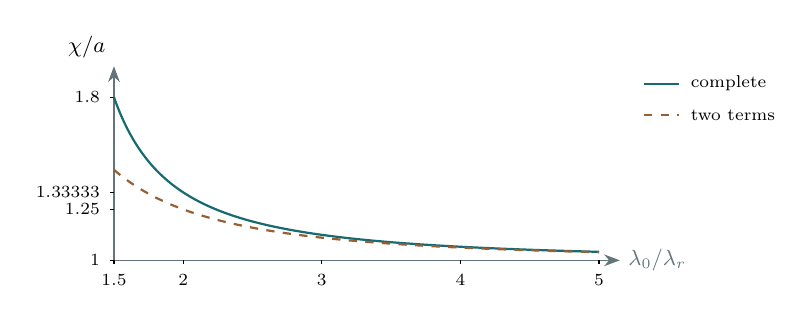
\begin{tikzpicture}[scale=.88,transform shape]
\draw[axis] (0,0)--(7.3,0) node[right] {$\lambda_0/\lambda_r$};
\draw[axis] (0,0)--(0,2.8);
\node[above left] at (0,2.8) {$\chi/a$};
\draw[thin] (0.000000,0)--(0.000000,-0.06);\node[below,font=\scriptsize] at (0.000000,-0.08) {$ 1.5 $};
\draw[thin] (1.000000,0)--(1.000000,-0.06);\node[below,font=\scriptsize] at (1.000000,-0.08) {$ 2 $};
\draw[thin] (3.000000,0)--(3.000000,-0.06);\node[below,font=\scriptsize] at (3.000000,-0.08) {$ 3 $};
\draw[thin] (5.000000,0)--(5.000000,-0.06);\node[below,font=\scriptsize] at (5.000000,-0.08) {$ 4 $};
\draw[thin] (7.000000,0)--(7.000000,-0.06);\node[below,font=\scriptsize] at (7.000000,-0.08) {$ 5 $};
\draw[thin] (0,0.000000)--(-.06,0.000000);\node[left,font=\scriptsize] at (-.08,0.000000) {$ 1 $};
\draw[thin] (0,0.735294)--(-.06,0.735294);\node[left,font=\scriptsize] at (-.08,0.735294) {$ 1.25 $};
\draw[thin] (0,0.980391)--(-.06,0.980391);\node[left,font=\scriptsize] at (-.08,0.980391) {$ 1.33333 $};
\draw[thin] (0,2.352941)--(-.06,2.352941);\node[left,font=\scriptsize] at (-.08,2.352941) {$ 1.8 $};
\draw[thick,color=accent] plot coordinates {(0.0000000,2.3529412) (0.0291667,2.2729995) (0.0583333,2.1976127) (0.0875000,2.1264119) (0.1166667,2.0590666) (0.1458333,1.9952803) (0.1750000,1.9347856) (0.2041667,1.8773415) (0.2333333,1.8227294) (0.2625000,1.7707513) (0.2916667,1.7212270) (0.3208333,1.6739921) (0.3500000,1.6288966) (0.3791667,1.5858033) (0.4083333,1.5445863) (0.4375000,1.5051298) (0.4666667,1.4673275) (0.4958333,1.4310813) (0.5250000,1.3963007) (0.5541667,1.3629018) (0.5833333,1.3308073) (0.6125000,1.2999451) (0.6416667,1.2702484) (0.6708333,1.2416553) (0.7000000,1.2141079) (0.7291667,1.1875523) (0.7583333,1.1619383) (0.7875000,1.1372188) (0.8166667,1.1133498) (0.8458333,1.0902903) (0.8750000,1.0680017) (0.9041667,1.0464477) (0.9333333,1.0255943) (0.9625000,1.0054096) (0.9916667,0.9858635) (1.0208333,0.9669276) (1.0500000,0.9485754) (1.0791667,0.9307815) (1.1083333,0.9135221) (1.1375000,0.8967749) (1.1666667,0.8805185) (1.1958333,0.8647329) (1.2250000,0.8493989) (1.2541667,0.8344986) (1.2833333,0.8200147) (1.3125000,0.8059311) (1.3416667,0.7922324) (1.3708333,0.7789038) (1.4000000,0.7659314) (1.4291667,0.7533019) (1.4583333,0.7410028) (1.4875000,0.7290220) (1.5166667,0.7173480) (1.5458333,0.7059699) (1.5750000,0.6948772) (1.6041667,0.6840601) (1.6333333,0.6735090) (1.6625000,0.6632148) (1.6916667,0.6531689) (1.7208333,0.6433629) (1.7500000,0.6337889) (1.7791667,0.6244392) (1.8083333,0.6153067) (1.8375000,0.6063842) (1.8666667,0.5976651) (1.8958333,0.5891430) (1.9250000,0.5808118) (1.9541667,0.5726655) (1.9833333,0.5646984) (2.0125000,0.5569050) (2.0416667,0.5492803) (2.0708333,0.5418190) (2.1000000,0.5345164) (2.1291667,0.5273678) (2.1583333,0.5203687) (2.1875000,0.5135149) (2.2166667,0.5068021) (2.2458333,0.5002263) (2.2750000,0.4937837) (2.3041667,0.4874706) (2.3333333,0.4812834) (2.3625000,0.4752186) (2.3916667,0.4692730) (2.4208333,0.4634432) (2.4500000,0.4577261) (2.4791667,0.4521189) (2.5083333,0.4466185) (2.5375000,0.4412221) (2.5666667,0.4359272) (2.5958333,0.4307310) (2.6250000,0.4256310) (2.6541667,0.4206247) (2.6833333,0.4157099) (2.7125000,0.4108842) (2.7416667,0.4061454) (2.7708333,0.4014913) (2.8000000,0.3969199) (2.8291667,0.3924292) (2.8583333,0.3880171) (2.8875000,0.3836819) (2.9166667,0.3794216) (2.9458333,0.3752346) (2.9750000,0.3711191) (3.0041667,0.3670733) (3.0333333,0.3630958) (3.0625000,0.3591848) (3.0916667,0.3553390) (3.1208333,0.3515567) (3.1500000,0.3478367) (3.1791667,0.3441774) (3.2083333,0.3405775) (3.2375000,0.3370357) (3.2666667,0.3335508) (3.2958333,0.3301214) (3.3250000,0.3267463) (3.3541667,0.3234245) (3.3833333,0.3201547) (3.4125000,0.3169358) (3.4416667,0.3137667) (3.4708333,0.3106465) (3.5000000,0.3075740) (3.5291667,0.3045483) (3.5583333,0.3015684) (3.5875000,0.2986333) (3.6166667,0.2957422) (3.6458333,0.2928941) (3.6750000,0.2900881) (3.7041667,0.2873235) (3.7333333,0.2845994) (3.7625000,0.2819149) (3.7916667,0.2792693) (3.8208333,0.2766619) (3.8500000,0.2740918) (3.8791667,0.2715584) (3.9083333,0.2690609) (3.9375000,0.2665986) (3.9666667,0.2641709) (3.9958333,0.2617771) (4.0250000,0.2594166) (4.0541667,0.2570887) (4.0833333,0.2547928) (4.1125000,0.2525284) (4.1416667,0.2502948) (4.1708333,0.2480914) (4.2000000,0.2459178) (4.2291667,0.2437733) (4.2583333,0.2416574) (4.2875000,0.2395697) (4.3166667,0.2375096) (4.3458333,0.2354765) (4.3750000,0.2334701) (4.4041667,0.2314899) (4.4333333,0.2295353) (4.4625000,0.2276060) (4.4916667,0.2257015) (4.5208333,0.2238213) (4.5500000,0.2219651) (4.5791667,0.2201324) (4.6083333,0.2183229) (4.6375000,0.2165360) (4.6666667,0.2147715) (4.6958333,0.2130290) (4.7250000,0.2113080) (4.7541667,0.2096083) (4.7833333,0.2079294) (4.8125000,0.2062711) (4.8416667,0.2046330) (4.8708333,0.2030147) (4.9000000,0.2014160) (4.9291667,0.1998364) (4.9583333,0.1982758) (4.9875000,0.1967337) (5.0166667,0.1952099) (5.0458333,0.1937042) (5.0750000,0.1922161) (5.1041667,0.1907455) (5.1333333,0.1892920) (5.1625000,0.1878554) (5.1916667,0.1864354) (5.2208333,0.1850317) (5.2500000,0.1836442) (5.2791667,0.1822725) (5.3083333,0.1809164) (5.3375000,0.1795757) (5.3666667,0.1782501) (5.3958333,0.1769394) (5.4250000,0.1756434) (5.4541667,0.1743619) (5.4833333,0.1730945) (5.5125000,0.1718412) (5.5416667,0.1706017) (5.5708333,0.1693758) (5.6000000,0.1681633) (5.6291667,0.1669640) (5.6583333,0.1657778) (5.6875000,0.1646043) (5.7166667,0.1634435) (5.7458333,0.1622951) (5.7750000,0.1611590) (5.8041667,0.1600350) (5.8333333,0.1589229) (5.8625000,0.1578225) (5.8916667,0.1567337) (5.9208333,0.1556564) (5.9500000,0.1545903) (5.9791667,0.1535353) (6.0083333,0.1524912) (6.0375000,0.1514579) (6.0666667,0.1504353) (6.0958333,0.1494231) (6.1250000,0.1484213) (6.1541667,0.1474297) (6.1833333,0.1464481) (6.2125000,0.1454765) (6.2416667,0.1445146) (6.2708333,0.1435624) (6.3000000,0.1426198) (6.3291667,0.1416865) (6.3583333,0.1407625) (6.3875000,0.1398477) (6.4166667,0.1389418) (6.4458333,0.1380449) (6.4750000,0.1371567) (6.5041667,0.1362773) (6.5333333,0.1354064) (6.5625000,0.1345439) (6.5916667,0.1336897) (6.6208333,0.1328438) (6.6500000,0.1320060) (6.6791667,0.1311762) (6.7083333,0.1303543) (6.7375000,0.1295403) (6.7666667,0.1287339) (6.7958333,0.1279352) (6.8250000,0.1271439) (6.8541667,0.1263601) (6.8833333,0.1255836) (6.9125000,0.1248143) (6.9416667,0.1240522) (6.9708333,0.1232971) (7.0000000,0.1225490)};
\draw[thick,color=accent] (7.65,2.55)--(8.15,2.55);\node[right,font=\scriptsize] at (8.2,2.55) {$\mathrm{complete}$};
\draw[thick,dashed,color=warm] plot coordinates {(0.0000000,1.3071895) (0.0291667,1.2821379) (0.0583333,1.2577996) (0.0875000,1.2341477) (0.1166667,1.2111568) (0.1458333,1.1888023) (0.1750000,1.1670612) (0.2041667,1.1459110) (0.2333333,1.1253306) (0.2625000,1.1052997) (0.2916667,1.0857988) (0.3208333,1.0668096) (0.3500000,1.0483142) (0.3791667,1.0302956) (0.4083333,1.0127376) (0.4375000,0.9956247) (0.4666667,0.9789419) (0.4958333,0.9626749) (0.5250000,0.9468100) (0.5541667,0.9313341) (0.5833333,0.9162345) (0.6125000,0.9014992) (0.6416667,0.8871166) (0.6708333,0.8730754) (0.7000000,0.8593649) (0.7291667,0.8459749) (0.7583333,0.8328954) (0.7875000,0.8201170) (0.8166667,0.8076303) (0.8458333,0.7954267) (0.8750000,0.7834976) (0.9041667,0.7718348) (0.9333333,0.7604306) (0.9625000,0.7492772) (0.9916667,0.7383674) (1.0208333,0.7276942) (1.0500000,0.7172508) (1.0791667,0.7070305) (1.1083333,0.6970272) (1.1375000,0.6872347) (1.1666667,0.6776471) (1.1958333,0.6682587) (1.2250000,0.6590641) (1.2541667,0.6500579) (1.2833333,0.6412352) (1.3125000,0.6325908) (1.3416667,0.6241200) (1.3708333,0.6158183) (1.4000000,0.6076811) (1.4291667,0.5997041) (1.4583333,0.5918832) (1.4875000,0.5842143) (1.5166667,0.5766934) (1.5458333,0.5693169) (1.5750000,0.5620810) (1.6041667,0.5549821) (1.6333333,0.5480169) (1.6625000,0.5411821) (1.6916667,0.5344742) (1.7208333,0.5278904) (1.7500000,0.5214274) (1.7791667,0.5150824) (1.8083333,0.5088525) (1.8375000,0.5027350) (1.8666667,0.4967271) (1.8958333,0.4908263) (1.9250000,0.4850300) (1.9541667,0.4793358) (1.9833333,0.4737412) (2.0125000,0.4682441) (2.0416667,0.4628421) (2.0708333,0.4575330) (2.1000000,0.4523147) (2.1291667,0.4471852) (2.1583333,0.4421425) (2.1875000,0.4371846) (2.2166667,0.4323096) (2.2458333,0.4275157) (2.2750000,0.4228011) (2.3041667,0.4181641) (2.3333333,0.4136029) (2.3625000,0.4091160) (2.3916667,0.4047017) (2.4208333,0.4003584) (2.4500000,0.3960847) (2.4791667,0.3918791) (2.5083333,0.3877400) (2.5375000,0.3836662) (2.5666667,0.3796563) (2.5958333,0.3757089) (2.6250000,0.3718228) (2.6541667,0.3679966) (2.6833333,0.3642292) (2.7125000,0.3605194) (2.7416667,0.3568660) (2.7708333,0.3532678) (2.8000000,0.3497237) (2.8291667,0.3462327) (2.8583333,0.3427938) (2.8875000,0.3394058) (2.9166667,0.3360678) (2.9458333,0.3327788) (2.9750000,0.3295378) (3.0041667,0.3263440) (3.0333333,0.3231963) (3.0625000,0.3200940) (3.0916667,0.3170362) (3.1208333,0.3140219) (3.1500000,0.3110505) (3.1791667,0.3081210) (3.2083333,0.3052327) (3.2375000,0.3023848) (3.2666667,0.2995766) (3.2958333,0.2968073) (3.3250000,0.2940763) (3.3541667,0.2913828) (3.3833333,0.2887261) (3.4125000,0.2861056) (3.4416667,0.2835206) (3.4708333,0.2809704) (3.5000000,0.2784546) (3.5291667,0.2759723) (3.5583333,0.2735232) (3.5875000,0.2711064) (3.6166667,0.2687216) (3.6458333,0.2663681) (3.6750000,0.2640454) (3.7041667,0.2617529) (3.7333333,0.2594901) (3.7625000,0.2572566) (3.7916667,0.2550518) (3.8208333,0.2528752) (3.8500000,0.2507263) (3.8791667,0.2486047) (3.9083333,0.2465100) (3.9375000,0.2444416) (3.9666667,0.2423991) (3.9958333,0.2403821) (4.0250000,0.2383902) (4.0541667,0.2364230) (4.0833333,0.2344800) (4.1125000,0.2325608) (4.1416667,0.2306651) (4.1708333,0.2287925) (4.2000000,0.2269426) (4.2291667,0.2251151) (4.2583333,0.2233095) (4.2875000,0.2215256) (4.3166667,0.2197630) (4.3458333,0.2180213) (4.3750000,0.2163003) (4.4041667,0.2145995) (4.4333333,0.2129187) (4.4625000,0.2112576) (4.4916667,0.2096159) (4.5208333,0.2079932) (4.5500000,0.2063893) (4.5791667,0.2048039) (4.6083333,0.2032366) (4.6375000,0.2016873) (4.6666667,0.2001557) (4.6958333,0.1986414) (4.7250000,0.1971442) (4.7541667,0.1956639) (4.7833333,0.1942003) (4.8125000,0.1927529) (4.8416667,0.1913217) (4.8708333,0.1899064) (4.9000000,0.1885067) (4.9291667,0.1871225) (4.9583333,0.1857534) (4.9875000,0.1843993) (5.0166667,0.1830600) (5.0458333,0.1817352) (5.0750000,0.1804247) (5.1041667,0.1791284) (5.1333333,0.1778459) (5.1625000,0.1765772) (5.1916667,0.1753220) (5.2208333,0.1740802) (5.2500000,0.1728515) (5.2791667,0.1716358) (5.3083333,0.1704328) (5.3375000,0.1692425) (5.3666667,0.1680646) (5.3958333,0.1668989) (5.4250000,0.1657453) (5.4541667,0.1646037) (5.4833333,0.1634737) (5.5125000,0.1623554) (5.5416667,0.1612486) (5.5708333,0.1601530) (5.6000000,0.1590685) (5.6291667,0.1579950) (5.6583333,0.1569323) (5.6875000,0.1558804) (5.7166667,0.1548389) (5.7458333,0.1538079) (5.7750000,0.1527871) (5.8041667,0.1517765) (5.8333333,0.1507759) (5.8625000,0.1497851) (5.8916667,0.1488040) (5.9208333,0.1478326) (5.9500000,0.1468706) (5.9791667,0.1459180) (6.0083333,0.1449747) (6.0375000,0.1440404) (6.0666667,0.1431152) (6.0958333,0.1421989) (6.1250000,0.1412913) (6.1541667,0.1403924) (6.1833333,0.1395020) (6.2125000,0.1386201) (6.2416667,0.1377465) (6.2708333,0.1368811) (6.3000000,0.1360239) (6.3291667,0.1351747) (6.3583333,0.1343334) (6.3875000,0.1335000) (6.4166667,0.1326743) (6.4458333,0.1318562) (6.4750000,0.1310457) (6.5041667,0.1302426) (6.5333333,0.1294469) (6.5625000,0.1286584) (6.5916667,0.1278771) (6.6208333,0.1271030) (6.6500000,0.1263358) (6.6791667,0.1255756) (6.7083333,0.1248222) (6.7375000,0.1240755) (6.7666667,0.1233356) (6.7958333,0.1226022) (6.8250000,0.1218754) (6.8541667,0.1211550) (6.8833333,0.1204410) (6.9125000,0.1197332) (6.9416667,0.1190317) (6.9708333,0.1183363) (7.0000000,0.1176471)};
\draw[thick,dashed,color=warm] (7.65,2.0999999999999996)--(8.15,2.0999999999999996);\node[right,font=\scriptsize] at (8.2,2.0999999999999996) {$\mathrm{two\ terms}$};
\end{tikzpicture}
\figcaption{变图光5.2V2\quad 二倍共振波长处完整值4/3而两项式5/4}
\end{minipage}\end{center}
\item \textbf{用已知电子质量描述强度。}指定$|q|=e,m=m_e$，用有效强度$f$拟合同一组长波系数，求$f$及其与采用振子数的关系。

由$\chi=Nfe^2/[\varepsilon_0m_e(\omega_r^2-\omega^2)]$，测量固定的是$Nf$。取每原子一个电子振子时，$f=(q^2/m)_{\rm eff}/(e^2/m_e)=.72277\simeq.723$。变图光5.2V3以$N'=\sigma N$表示其他有效计数，得到$f'=f/\sigma$；例如$\sigma=1/2$给$f'=1.44553$。每个有效振子承担的权重随计数约定改变，总光学响应保持相同。
\begin{center}\begin{minipage}{.98\linewidth}\centering
\begin{tikzpicture}[scale=.88,transform shape]
\draw[axis] (0,0.0)--(7.3,0.0) node[right] {$N^\prime/N$};
\draw[axis] (0,0)--(0,2.8);
\node[above left] at (0,2.8) {$f^\prime$};
\draw[thin] (0.000000,0.0)--(0.000000,-0.06);\node[below,font=\scriptsize] at (0.000000,-0.08) {$ 0.5 $};
\draw[thin] (2.333333,0.0)--(2.333333,-0.06);\node[below,font=\scriptsize] at (2.333333,-0.08) {$ 1 $};
\draw[thin] (4.666667,0.0)--(4.666667,-0.06);\node[below,font=\scriptsize] at (4.666667,-0.08) {$ 1.5 $};
\draw[thin] (7.000000,0.0)--(7.000000,-0.06);\node[below,font=\scriptsize] at (7.000000,-0.08) {$ 2 $};
\draw[thin] (0,0.000000)--(-.06,0.000000);\node[left,font=\scriptsize] at (-.08,0.000000) {$ 0 $};
\draw[thin] (0,0.833333)--(-.06,0.833333);\node[left,font=\scriptsize] at (-.08,0.833333) {$ 0.5 $};
\draw[thin] (0,1.204617)--(-.06,1.204617);\node[left,font=\scriptsize] at (-.08,1.204617) {$ 0.72277 $};
\draw[thin] (0,1.666667)--(-.06,1.666667);\node[left,font=\scriptsize] at (-.08,1.666667) {$ 1 $};
\draw[thin] (0,2.409217)--(-.06,2.409217);\node[left,font=\scriptsize] at (-.08,2.409217) {$ 1.44553 $};
\draw[thick,color=accent] plot coordinates {(0.0000000,2.4092247) (0.0291667,2.3794812) (0.0583333,2.3504631) (0.0875000,2.3221443) (0.1166667,2.2944997) (0.1458333,2.2675056) (0.1750000,2.2411393) (0.2041667,2.2153790) (0.2333333,2.1902043) (0.2625000,2.1655952) (0.2916667,2.1415331) (0.3208333,2.1179997) (0.3500000,2.0949780) (0.3791667,2.0724514) (0.4083333,2.0504040) (0.4375000,2.0288208) (0.4666667,2.0076872) (0.4958333,1.9869894) (0.5250000,1.9667140) (0.5541667,1.9468482) (0.5833333,1.9273798) (0.6125000,1.9082968) (0.6416667,1.8895880) (0.6708333,1.8712425) (0.7000000,1.8532498) (0.7291667,1.8355998) (0.7583333,1.8182828) (0.7875000,1.8012895) (0.8166667,1.7846109) (0.8458333,1.7682383) (0.8750000,1.7521634) (0.9041667,1.7363782) (0.9333333,1.7208748) (0.9625000,1.7056458) (0.9916667,1.6906840) (1.0208333,1.6759824) (1.0500000,1.6615343) (1.0791667,1.6473331) (1.1083333,1.6333727) (1.1375000,1.6196469) (1.1666667,1.6061498) (1.1958333,1.5928758) (1.2250000,1.5798195) (1.2541667,1.5669754) (1.2833333,1.5543385) (1.3125000,1.5419038) (1.3416667,1.5296665) (1.3708333,1.5176219) (1.4000000,1.5057654) (1.4291667,1.4940928) (1.4583333,1.4825998) (1.4875000,1.4712823) (1.5166667,1.4601362) (1.5458333,1.4491577) (1.5750000,1.4383431) (1.6041667,1.4276887) (1.6333333,1.4171910) (1.6625000,1.4068465) (1.6916667,1.3966520) (1.7208333,1.3866041) (1.7500000,1.3766998) (1.7791667,1.3669360) (1.8083333,1.3573097) (1.8375000,1.3478180) (1.8666667,1.3384582) (1.8958333,1.3292274) (1.9250000,1.3201231) (1.9541667,1.3111427) (1.9833333,1.3022836) (2.0125000,1.2935435) (2.0416667,1.2849198) (2.0708333,1.2764104) (2.1000000,1.2680130) (2.1291667,1.2597253) (2.1583333,1.2515453) (2.1875000,1.2434708) (2.2166667,1.2354998) (2.2458333,1.2276304) (2.2750000,1.2198606) (2.3041667,1.2121885) (2.3333333,1.2046123) (2.3625000,1.1971303) (2.3916667,1.1897406) (2.4208333,1.1824416) (2.4500000,1.1752316) (2.4791667,1.1681089) (2.5083333,1.1610721) (2.5375000,1.1541196) (2.5666667,1.1472499) (2.5958333,1.1404614) (2.6250000,1.1337528) (2.6541667,1.1271227) (2.6833333,1.1205696) (2.7125000,1.1140923) (2.7416667,1.1076895) (2.7708333,1.1013599) (2.8000000,1.0951021) (2.8291667,1.0889151) (2.8583333,1.0827976) (2.8875000,1.0767485) (2.9166667,1.0707665) (2.9458333,1.0648507) (2.9750000,1.0589999) (3.0041667,1.0532130) (3.0333333,1.0474890) (3.0625000,1.0418269) (3.0916667,1.0362257) (3.1208333,1.0306844) (3.1500000,1.0252020) (3.1791667,1.0197777) (3.2083333,1.0144104) (3.2375000,1.0090994) (3.2666667,1.0038436) (3.2958333,0.9986424) (3.3250000,0.9934947) (3.3541667,0.9883999) (3.3833333,0.9833570) (3.4125000,0.9783654) (3.4416667,0.9734241) (3.4708333,0.9685325) (3.5000000,0.9636899) (3.5291667,0.9588954) (3.5583333,0.9541484) (3.5875000,0.9494482) (3.6166667,0.9447940) (3.6458333,0.9401852) (3.6750000,0.9356212) (3.7041667,0.9311013) (3.7333333,0.9266249) (3.7625000,0.9221913) (3.7916667,0.9177999) (3.8208333,0.9134501) (3.8500000,0.9091414) (3.8791667,0.9048731) (3.9083333,0.9006447) (3.9375000,0.8964557) (3.9666667,0.8923054) (3.9958333,0.8881934) (4.0250000,0.8841192) (4.0541667,0.8800821) (4.0833333,0.8760817) (4.1125000,0.8721175) (4.1416667,0.8681891) (4.1708333,0.8642959) (4.2000000,0.8604374) (4.2291667,0.8566132) (4.2583333,0.8528229) (4.2875000,0.8490660) (4.3166667,0.8453420) (4.3458333,0.8416505) (4.3750000,0.8379912) (4.4041667,0.8343635) (4.4333333,0.8307671) (4.4625000,0.8272016) (4.4916667,0.8236666) (4.5208333,0.8201616) (4.5500000,0.8166863) (4.5791667,0.8132404) (4.6083333,0.8098234) (4.6375000,0.8064350) (4.6666667,0.8030749) (4.6958333,0.7997426) (4.7250000,0.7964379) (4.7541667,0.7931604) (4.7833333,0.7899097) (4.8125000,0.7866856) (4.8416667,0.7834877) (4.8708333,0.7803157) (4.9000000,0.7771693) (4.9291667,0.7740481) (4.9583333,0.7709519) (4.9875000,0.7678804) (5.0166667,0.7648332) (5.0458333,0.7618102) (5.0750000,0.7588109) (5.1041667,0.7558352) (5.1333333,0.7528827) (5.1625000,0.7499532) (5.1916667,0.7470464) (5.2208333,0.7441621) (5.2500000,0.7412999) (5.2791667,0.7384597) (5.3083333,0.7356411) (5.3375000,0.7328440) (5.3666667,0.7300681) (5.3958333,0.7273131) (5.4250000,0.7245789) (5.4541667,0.7218651) (5.4833333,0.7191716) (5.5125000,0.7164981) (5.5416667,0.7138444) (5.5708333,0.7112102) (5.6000000,0.7085955) (5.6291667,0.7059999) (5.6583333,0.7034233) (5.6875000,0.7008654) (5.7166667,0.6983260) (5.7458333,0.6958050) (5.7750000,0.6933021) (5.8041667,0.6908171) (5.8333333,0.6883499) (5.8625000,0.6859003) (5.8916667,0.6834680) (5.9208333,0.6810529) (5.9500000,0.6786548) (5.9791667,0.6762736) (6.0083333,0.6739090) (6.0375000,0.6715609) (6.0666667,0.6692291) (6.0958333,0.6669134) (6.1250000,0.6646137) (6.1541667,0.6623298) (6.1833333,0.6600616) (6.2125000,0.6578088) (6.2416667,0.6555713) (6.2708333,0.6533491) (6.3000000,0.6511418) (6.3291667,0.6489494) (6.3583333,0.6467717) (6.3875000,0.6446086) (6.4166667,0.6424599) (6.4458333,0.6403255) (6.4750000,0.6382052) (6.5041667,0.6360989) (6.5333333,0.6340065) (6.5625000,0.6319278) (6.5916667,0.6298627) (6.6208333,0.6278110) (6.6500000,0.6257726) (6.6791667,0.6237475) (6.7083333,0.6217354) (6.7375000,0.6197363) (6.7666667,0.6177499) (6.7958333,0.6157763) (6.8250000,0.6138152) (6.8541667,0.6118666) (6.8833333,0.6099303) (6.9125000,0.6080062) (6.9416667,0.6060943) (6.9708333,0.6041943) (7.0000000,0.6023062)};
\end{tikzpicture}
\figcaption{变图光5.2V3\quad 相同总响应下每个有效振子的权重与计数成反比}
\end{minipage}\end{center}
\item \textbf{加入阻尼后的复响应。}取$\Gamma=\gamma/\omega_r=.05$，求$u=\omega/\omega_r$处响应的实、虚部，给共振点数值，并说明峰宽尺度。

将分母乘共轭，得
\[
 \frac{\chi'}a=\frac{1-u^2}{(1-u^2)^2+\Gamma^2u^2},\qquad
 \frac{\chi''}a=\frac{\Gamma u}{(1-u^2)^2+\Gamma^2u^2}.
\]
变图光5.2V4中$u=1$处$\chi'=0,\chi''/a=1/\Gamma=20$，虚部为正。在$u=1+s$、$|s|\ll1$时，$\chi''/a\simeq\Gamma/(4s^2+\Gamma^2)$，半高位置$s\simeq\pm\Gamma/2$，故小阻尼的半高全宽约为$\Delta\omega=\gamma$。峰位尺度由长波系数给出，阻尼决定有限峰宽。
\begin{center}\begin{minipage}{.98\linewidth}\centering
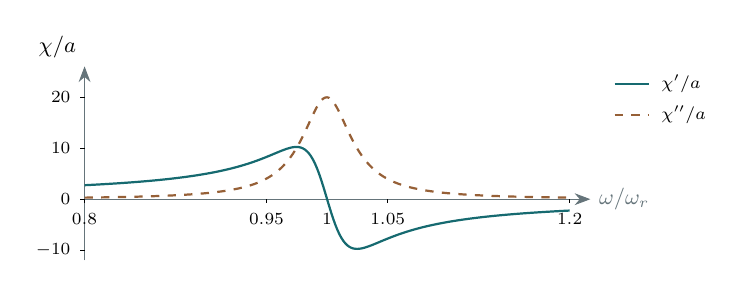
\begin{tikzpicture}[scale=.88,transform shape]
\draw[axis] (0,0.8823529411764706)--(7.3,0.8823529411764706) node[right] {$\omega/\omega_r$};
\draw[axis] (0,0)--(0,2.8);
\node[above left] at (0,2.8) {$\chi/a$};
\draw[thin] (0.000000,0.8823529411764706)--(0.000000,0.8223529411764705);\node[below,font=\scriptsize] at (0.000000,0.8023529411764706) {$ 0.8 $};
\draw[thin] (2.625000,0.8823529411764706)--(2.625000,0.8223529411764705);\node[below,font=\scriptsize] at (2.625000,0.8023529411764706) {$ 0.95 $};
\draw[thin] (3.500000,0.8823529411764706)--(3.500000,0.8223529411764705);\node[below,font=\scriptsize] at (3.500000,0.8023529411764706) {$ 1 $};
\draw[thin] (4.375000,0.8823529411764706)--(4.375000,0.8223529411764705);\node[below,font=\scriptsize] at (4.375000,0.8023529411764706) {$ 1.05 $};
\draw[thin] (7.000000,0.8823529411764706)--(7.000000,0.8223529411764705);\node[below,font=\scriptsize] at (7.000000,0.8023529411764706) {$ 1.2 $};
\draw[thin] (0,0.147059)--(-.06,0.147059);\node[left,font=\scriptsize] at (-.08,0.147059) {$ -10 $};
\draw[thin] (0,0.882353)--(-.06,0.882353);\node[left,font=\scriptsize] at (-.08,0.882353) {$ 0 $};
\draw[thin] (0,1.617647)--(-.06,1.617647);\node[left,font=\scriptsize] at (-.08,1.617647) {$ 10 $};
\draw[thin] (0,2.352941)--(-.06,2.352941);\node[left,font=\scriptsize] at (-.08,2.352941) {$ 20 $};
\draw[thick,color=accent] plot coordinates {(0.0000000,1.0841105) (0.0291667,1.0855700) (0.0583333,1.0870536) (0.0875000,1.0885616) (0.1166667,1.0900947) (0.1458333,1.0916535) (0.1750000,1.0932386) (0.2041667,1.0948507) (0.2333333,1.0964905) (0.2625000,1.0981586) (0.2916667,1.0998558) (0.3208333,1.1015828) (0.3500000,1.1033403) (0.3791667,1.1051292) (0.4083333,1.1069503) (0.4375000,1.1088044) (0.4666667,1.1106923) (0.4958333,1.1126151) (0.5250000,1.1145736) (0.5541667,1.1165687) (0.5833333,1.1186016) (0.6125000,1.1206732) (0.6416667,1.1227846) (0.6708333,1.1249369) (0.7000000,1.1271313) (0.7291667,1.1293689) (0.7583333,1.1316510) (0.7875000,1.1339790) (0.8166667,1.1363540) (0.8458333,1.1387776) (0.8750000,1.1412511) (0.9041667,1.1437760) (0.9333333,1.1463540) (0.9625000,1.1489865) (0.9916667,1.1516753) (1.0208333,1.1544220) (1.0500000,1.1572286) (1.0791667,1.1600969) (1.1083333,1.1630288) (1.1375000,1.1660263) (1.1666667,1.1690916) (1.1958333,1.1722269) (1.2250000,1.1754344) (1.2541667,1.1787166) (1.2833333,1.1820759) (1.3125000,1.1855149) (1.3416667,1.1890363) (1.3708333,1.1926429) (1.4000000,1.1963376) (1.4291667,1.2001234) (1.4583333,1.2040036) (1.4875000,1.2079814) (1.5166667,1.2120603) (1.5458333,1.2162438) (1.5750000,1.2205358) (1.6041667,1.2249401) (1.6333333,1.2294607) (1.6625000,1.2341020) (1.6916667,1.2388683) (1.7208333,1.2437643) (1.7500000,1.2487946) (1.7791667,1.2539643) (1.8083333,1.2592787) (1.8375000,1.2647429) (1.8666667,1.2703627) (1.8958333,1.2761439) (1.9250000,1.2820924) (1.9541667,1.2882145) (1.9833333,1.2945165) (2.0125000,1.3010052) (2.0416667,1.3076872) (2.0708333,1.3145697) (2.1000000,1.3216596) (2.1291667,1.3289643) (2.1583333,1.3364910) (2.1875000,1.3442472) (2.2166667,1.3522401) (2.2458333,1.3604770) (2.2750000,1.3689649) (2.3041667,1.3777106) (2.3333333,1.3867203) (2.3625000,1.3959995) (2.3916667,1.4055531) (2.4208333,1.4153845) (2.4500000,1.4254958) (2.4791667,1.4358872) (2.5083333,1.4465565) (2.5375000,1.4574982) (2.5666667,1.4687033) (2.5958333,1.4801578) (2.6250000,1.4918422) (2.6541667,1.5037295) (2.6833333,1.5157838) (2.7125000,1.5279585) (2.7416667,1.5401937) (2.7708333,1.5524132) (2.8000000,1.5645214) (2.8291667,1.5763990) (2.8583333,1.5878980) (2.8875000,1.5988364) (2.9166667,1.6089917) (2.9458333,1.6180937) (2.9750000,1.6258164) (3.0041667,1.6317697) (3.0333333,1.6354914) (3.0625000,1.6364396) (3.0916667,1.6339874) (3.1208333,1.6274221) (3.1500000,1.6159502) (3.1791667,1.5987126) (3.2083333,1.5748128) (3.2375000,1.5433624) (3.2666667,1.5035458) (3.2958333,1.4547055) (3.3250000,1.3964435) (3.3541667,1.3287301) (3.3833333,1.2520035) (3.4125000,1.1672385) (3.4416667,1.0759627) (3.4708333,0.9802022) (3.5000000,0.8823529) (3.5291667,0.7849903) (3.5583333,0.6906473) (3.5875000,0.6016008) (3.6166667,0.5197011) (3.6458333,0.4462709) (3.6750000,0.3820784) (3.7041667,0.3273760) (3.7333333,0.2819834) (3.7625000,0.2453927) (3.7916667,0.2168759) (3.8208333,0.1955811) (3.8500000,0.1806105) (3.8791667,0.1710771) (3.9083333,0.1661440) (3.9375000,0.1650468) (3.9666667,0.1671049) (3.9958333,0.1717235) (4.0250000,0.1783915) (4.0541667,0.1866745) (4.0833333,0.1962076) (4.1125000,0.2066866) (4.1416667,0.2178601) (4.1708333,0.2295216) (4.2000000,0.2415026) (4.2291667,0.2536664) (4.2583333,0.2659033) (4.2875000,0.2781251) (4.3166667,0.2902623) (4.3458333,0.3022603) (4.3750000,0.3140766) (4.4041667,0.3256791) (4.4333333,0.3370437) (4.4625000,0.3481530) (4.4916667,0.3589951) (4.5208333,0.3695624) (4.5500000,0.3798507) (4.5791667,0.3898588) (4.6083333,0.3995876) (4.6375000,0.4090398) (4.6666667,0.4182193) (4.6958333,0.4271314) (4.7250000,0.4357817) (4.7541667,0.4441769) (4.7833333,0.4523237) (4.8125000,0.4602293) (4.8416667,0.4679008) (4.8708333,0.4753458) (4.9000000,0.4825715) (4.9291667,0.4895853) (4.9583333,0.4963943) (4.9875000,0.5030056) (5.0166667,0.5094261) (5.0458333,0.5156626) (5.0750000,0.5217216) (5.1041667,0.5276094) (5.1333333,0.5333322) (5.1625000,0.5388960) (5.1916667,0.5443063) (5.2208333,0.5495688) (5.2500000,0.5546887) (5.2791667,0.5596712) (5.3083333,0.5645211) (5.3375000,0.5692432) (5.3666667,0.5738420) (5.3958333,0.5783219) (5.4250000,0.5826869) (5.4541667,0.5869412) (5.4833333,0.5910886) (5.5125000,0.5951327) (5.5416667,0.5990770) (5.5708333,0.6029251) (5.6000000,0.6066801) (5.6291667,0.6103451) (5.6583333,0.6139232) (5.6875000,0.6174172) (5.7166667,0.6208299) (5.7458333,0.6241639) (5.7750000,0.6274218) (5.8041667,0.6306060) (5.8333333,0.6337189) (5.8625000,0.6367627) (5.8916667,0.6397396) (5.9208333,0.6426517) (5.9500000,0.6455009) (5.9791667,0.6482892) (6.0083333,0.6510184) (6.0375000,0.6536904) (6.0666667,0.6563067) (6.0958333,0.6588692) (6.1250000,0.6613793) (6.1541667,0.6638386) (6.1833333,0.6662485) (6.2125000,0.6686105) (6.2416667,0.6709260) (6.2708333,0.6731962) (6.3000000,0.6754224) (6.3291667,0.6776059) (6.3583333,0.6797478) (6.3875000,0.6818492) (6.4166667,0.6839113) (6.4458333,0.6859351) (6.4750000,0.6879217) (6.5041667,0.6898720) (6.5333333,0.6917869) (6.5625000,0.6936675) (6.5916667,0.6955146) (6.6208333,0.6973290) (6.6500000,0.6991117) (6.6791667,0.7008633) (6.7083333,0.7025847) (6.7375000,0.7042767) (6.7666667,0.7059399) (6.7958333,0.7075751) (6.8250000,0.7091829) (6.8541667,0.7107641) (6.8833333,0.7123192) (6.9125000,0.7138489) (6.9416667,0.7153537) (6.9708333,0.7168344) (7.0000000,0.7182914)};
\draw[thick,color=accent] (7.65,2.55)--(8.15,2.55);\node[right,font=\scriptsize] at (8.2,2.55) {$\chi^\prime/a$};
\draw[thick,dashed,color=warm] plot coordinates {(0.0000000,0.9047704) (0.0291667,0.9051487) (0.0583333,0.9055364) (0.0875000,0.9059339) (0.1166667,0.9063414) (0.1458333,0.9067595) (0.1750000,0.9071883) (0.2041667,0.9076283) (0.2333333,0.9080798) (0.2625000,0.9085433) (0.2916667,0.9090193) (0.3208333,0.9095080) (0.3500000,0.9100101) (0.3791667,0.9105259) (0.4083333,0.9110561) (0.4375000,0.9116011) (0.4666667,0.9121614) (0.4958333,0.9127377) (0.5250000,0.9133306) (0.5541667,0.9139407) (0.5833333,0.9145687) (0.6125000,0.9152152) (0.6416667,0.9158810) (0.6708333,0.9165670) (0.7000000,0.9172738) (0.7291667,0.9180023) (0.7583333,0.9187535) (0.7875000,0.9195282) (0.8166667,0.9203275) (0.8458333,0.9211524) (0.8750000,0.9220040) (0.9041667,0.9228835) (0.9333333,0.9237920) (0.9625000,0.9247308) (0.9916667,0.9257013) (1.0208333,0.9267050) (1.0500000,0.9277433) (1.0791667,0.9288179) (1.1083333,0.9299303) (1.1375000,0.9310825) (1.1666667,0.9322762) (1.1958333,0.9335135) (1.2250000,0.9347966) (1.2541667,0.9361276) (1.2833333,0.9375089) (1.3125000,0.9389432) (1.3416667,0.9404330) (1.3708333,0.9419813) (1.4000000,0.9435911) (1.4291667,0.9452656) (1.4583333,0.9470084) (1.4875000,0.9488231) (1.5166667,0.9507136) (1.5458333,0.9526842) (1.5750000,0.9547394) (1.6041667,0.9568839) (1.6333333,0.9591230) (1.6625000,0.9614622) (1.6916667,0.9639074) (1.7208333,0.9664650) (1.7500000,0.9691418) (1.7791667,0.9719451) (1.8083333,0.9748829) (1.8375000,0.9779636) (1.8666667,0.9811966) (1.8958333,0.9845916) (1.9250000,0.9881595) (1.9541667,0.9919117) (1.9833333,0.9958609) (2.0125000,1.0000205) (2.0416667,1.0044054) (2.0708333,1.0090315) (2.1000000,1.0139161) (2.1291667,1.0190783) (2.1583333,1.0245384) (2.1875000,1.0303191) (2.2166667,1.0364446) (2.2458333,1.0429417) (2.2750000,1.0498397) (2.3041667,1.0571703) (2.3333333,1.0649687) (2.3625000,1.0732731) (2.3916667,1.0821254) (2.4208333,1.0915719) (2.4500000,1.1016632) (2.4791667,1.1124549) (2.5083333,1.1240081) (2.5375000,1.1363900) (2.5666667,1.1496745) (2.5958333,1.1639427) (2.6250000,1.1792836) (2.6541667,1.1957950) (2.6833333,1.2135838) (2.7125000,1.2327669) (2.7416667,1.2534713) (2.7708333,1.2758351) (2.8000000,1.3000071) (2.8291667,1.3261466) (2.8583333,1.3544223) (2.8875000,1.3850113) (2.9166667,1.4180951) (2.9458333,1.4538562) (2.9750000,1.4924710) (3.0041667,1.5341007) (3.0333333,1.5788788) (3.0625000,1.6268942) (3.0916667,1.6781692) (3.1208333,1.7326327) (3.1500000,1.7900869) (3.1791667,1.8501696) (3.2083333,1.9123143) (3.2375000,1.9757104) (3.2666667,2.0392726) (3.2958333,2.1016263) (3.3250000,2.1611208) (3.3541667,2.2158815) (3.3833333,2.2639066) (3.4125000,2.3032108) (3.4416667,2.3320017) (3.4708333,2.3488675) (3.5000000,2.3529412) (3.5291667,2.3440088) (3.5583333,2.3225372) (3.5875000,2.2896141) (3.6166667,2.2468153) (3.6458333,2.1960275) (3.6750000,2.1392617) (3.7041667,2.0784863) (3.7333333,2.0155008) (3.7625000,1.9518561) (3.7916667,1.8888183) (3.8208333,1.8273666) (3.8500000,1.7682160) (3.8791667,1.7118515) (3.9083333,1.6585691) (3.9375000,1.6085147) (3.9666667,1.5617210) (3.9958333,1.5181377) (4.0250000,1.4776570) (4.0541667,1.4401332) (4.0833333,1.4053982) (4.1125000,1.3732723) (4.1416667,1.3435728) (4.1708333,1.3161194) (4.2000000,1.2907380) (4.2291667,1.2672630) (4.2583333,1.2455392) (4.2875000,1.2254217) (4.3166667,1.2067767) (4.3458333,1.1894809) (4.3750000,1.1734213) (4.4041667,1.1584944) (4.4333333,1.1446060) (4.4625000,1.1316699) (4.4916667,1.1196078) (4.5208333,1.1083485) (4.5500000,1.0978272) (4.5791667,1.0879848) (4.6083333,1.0787675) (4.6375000,1.0701267) (4.6666667,1.0620176) (4.6958333,1.0543997) (4.7250000,1.0472360) (4.7541667,1.0404928) (4.7833333,1.0341391) (4.8125000,1.0281467) (4.8416667,1.0224898) (4.8708333,1.0171447) (4.9000000,1.0120897) (4.9291667,1.0073049) (4.9583333,1.0027720) (4.9875000,0.9984742) (5.0166667,0.9943960) (5.0458333,0.9905230) (5.0750000,0.9868421) (5.1041667,0.9833411) (5.1333333,0.9800089) (5.1625000,0.9768349) (5.1916667,0.9738096) (5.2208333,0.9709239) (5.2500000,0.9681698) (5.2791667,0.9655393) (5.3083333,0.9630254) (5.3375000,0.9606215) (5.3666667,0.9583213) (5.3958333,0.9561191) (5.4250000,0.9540094) (5.4541667,0.9519873) (5.4833333,0.9500480) (5.5125000,0.9481872) (5.5416667,0.9464007) (5.5708333,0.9446847) (5.6000000,0.9430357) (5.6291667,0.9414501) (5.6583333,0.9399249) (5.6875000,0.9384570) (5.7166667,0.9370437) (5.7458333,0.9356823) (5.7750000,0.9343703) (5.8041667,0.9331055) (5.8333333,0.9318855) (5.8625000,0.9307084) (5.8916667,0.9295721) (5.9208333,0.9284749) (5.9500000,0.9274149) (5.9791667,0.9263906) (6.0083333,0.9254003) (6.0375000,0.9244426) (6.0666667,0.9235161) (6.0958333,0.9226194) (6.1250000,0.9217513) (6.1541667,0.9209107) (6.1833333,0.9200963) (6.2125000,0.9193071) (6.2416667,0.9185421) (6.2708333,0.9178004) (6.3000000,0.9170809) (6.3291667,0.9163828) (6.3583333,0.9157053) (6.3875000,0.9150476) (6.4166667,0.9144089) (6.4458333,0.9137885) (6.4750000,0.9131858) (6.5041667,0.9126000) (6.5333333,0.9120305) (6.5625000,0.9114768) (6.5916667,0.9109383) (6.6208333,0.9104143) (6.6500000,0.9099045) (6.6791667,0.9094083) (6.7083333,0.9089252) (6.7375000,0.9084548) (6.7666667,0.9079966) (6.7958333,0.9075502) (6.8250000,0.9071153) (6.8541667,0.9066914) (6.8833333,0.9062781) (6.9125000,0.9058752) (6.9416667,0.9054823) (6.9708333,0.9050989) (7.0000000,0.9047250)};
\draw[thick,dashed,color=warm] (7.65,2.0999999999999996)--(8.15,2.0999999999999996);\node[right,font=\scriptsize] at (8.2,2.0999999999999996) {$\chi^{\prime\prime}/a$};
\end{tikzpicture}
\figcaption{变图光5.2V4\quad 实部过零与有限正虚部由同一阻尼分母给出}
\end{minipage}\end{center}
\item \textbf{两个紫外共振给相同长波系数。}设实际模型取70nm、110nm两个共振，静态响应权重为$a_1,a_2$。求使常数$a$和平方系数$b$与题设相同的权重比例。

长波展开给$a_1+a_2=a$、$a_1\lambda_1^2+a_2\lambda_2^2=b=a\lambda_r^2$。因此
\[
 \frac{a_2}a=\frac{\lambda_r^2-\lambda_1^2}{\lambda_2^2-\lambda_1^2}=.396459,
 \qquad a_1/a=.603541.
\]
变图光5.2V5比较两共振完整响应、88.06nm单有效共振和共同的两项展开。前两长波系数一致，下一阶项与近共振行为不同；这里88.06nm是静态权重下共振波长平方的均方尺度。
\begin{center}\begin{minipage}{.98\linewidth}\centering
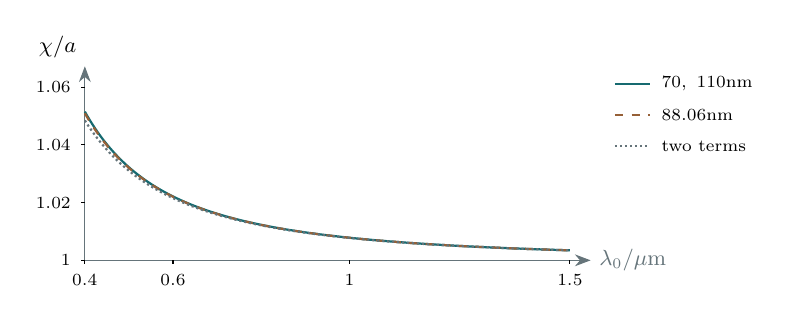
\begin{tikzpicture}[scale=.88,transform shape]
\draw[axis] (0,0)--(7.3,0) node[right] {$\lambda_0/{\rm \mu m}$};
\draw[axis] (0,0)--(0,2.8);
\node[above left] at (0,2.8) {$\chi/a$};
\draw[thin] (0.000000,0)--(0.000000,-0.06);\node[below,font=\scriptsize] at (0.000000,-0.08) {$ 0.4 $};
\draw[thin] (1.272727,0)--(1.272727,-0.06);\node[below,font=\scriptsize] at (1.272727,-0.08) {$ 0.6 $};
\draw[thin] (3.818182,0)--(3.818182,-0.06);\node[below,font=\scriptsize] at (3.818182,-0.08) {$ 1 $};
\draw[thin] (7.000000,0)--(7.000000,-0.06);\node[below,font=\scriptsize] at (7.000000,-0.08) {$ 1.5 $};
\draw[thin] (0,0.000000)--(-.06,0.000000);\node[left,font=\scriptsize] at (-.08,0.000000) {$ 1 $};
\draw[thin] (0,0.833333)--(-.06,0.833333);\node[left,font=\scriptsize] at (-.08,0.833333) {$ 1.02 $};
\draw[thin] (0,1.666667)--(-.06,1.666667);\node[left,font=\scriptsize] at (-.08,1.666667) {$ 1.04 $};
\draw[thin] (0,2.500000)--(-.06,2.500000);\node[left,font=\scriptsize] at (-.08,2.500000) {$ 1.06 $};
\draw[thick,color=accent] plot coordinates {(0.0000000,2.1459367) (0.0291667,2.0946088) (0.0583333,2.0451359) (0.0875000,1.9974279) (0.1166667,1.9514004) (0.1458333,1.9069741) (0.1750000,1.8640742) (0.2041667,1.8226306) (0.2333333,1.7825769) (0.2625000,1.7438507) (0.2916667,1.7063931) (0.3208333,1.6701484) (0.3500000,1.6350640) (0.3791667,1.6010903) (0.4083333,1.5681801) (0.4375000,1.5362889) (0.4666667,1.5053745) (0.4958333,1.4753968) (0.5250000,1.4463179) (0.5541667,1.4181017) (0.5833333,1.3907141) (0.6125000,1.3641224) (0.6416667,1.3382958) (0.6708333,1.3132049) (0.7000000,1.2888215) (0.7291667,1.2651191) (0.7583333,1.2420723) (0.7875000,1.2196568) (0.8166667,1.1978495) (0.8458333,1.1766283) (0.8750000,1.1559723) (0.9041667,1.1358613) (0.9333333,1.1162761) (0.9625000,1.0971984) (0.9916667,1.0786106) (1.0208333,1.0604959) (1.0500000,1.0428382) (1.0791667,1.0256221) (1.1083333,1.0088330) (1.1375000,0.9924566) (1.1666667,0.9764795) (1.1958333,0.9608885) (1.2250000,0.9456714) (1.2541667,0.9308161) (1.2833333,0.9163111) (1.3125000,0.9021454) (1.3416667,0.8883085) (1.3708333,0.8747901) (1.4000000,0.8615805) (1.4291667,0.8486703) (1.4583333,0.8360503) (1.4875000,0.8237120) (1.5166667,0.8116469) (1.5458333,0.7998470) (1.5750000,0.7883045) (1.6041667,0.7770118) (1.6333333,0.7659619) (1.6625000,0.7551477) (1.6916667,0.7445625) (1.7208333,0.7341998) (1.7500000,0.7240536) (1.7791667,0.7141176) (1.8083333,0.7043861) (1.8375000,0.6948535) (1.8666667,0.6855143) (1.8958333,0.6763634) (1.9250000,0.6673957) (1.9541667,0.6586063) (1.9833333,0.6499904) (2.0125000,0.6415435) (2.0416667,0.6332612) (2.0708333,0.6251393) (2.1000000,0.6171735) (2.1291667,0.6093598) (2.1583333,0.6016945) (2.1875000,0.5941737) (2.2166667,0.5867938) (2.2458333,0.5795514) (2.2750000,0.5724429) (2.3041667,0.5654651) (2.3333333,0.5586148) (2.3625000,0.5518889) (2.3916667,0.5452844) (2.4208333,0.5387983) (2.4500000,0.5324278) (2.4791667,0.5261703) (2.5083333,0.5200229) (2.5375000,0.5139832) (2.5666667,0.5080486) (2.5958333,0.5022167) (2.6250000,0.4964851) (2.6541667,0.4908515) (2.6833333,0.4853137) (2.7125000,0.4798696) (2.7416667,0.4745169) (2.7708333,0.4692537) (2.8000000,0.4640780) (2.8291667,0.4589878) (2.8583333,0.4539812) (2.8875000,0.4490565) (2.9166667,0.4442119) (2.9458333,0.4394455) (2.9750000,0.4347557) (3.0041667,0.4301410) (3.0333333,0.4255996) (3.0625000,0.4211300) (3.0916667,0.4167308) (3.1208333,0.4124004) (3.1500000,0.4081375) (3.1791667,0.4039405) (3.2083333,0.3998082) (3.2375000,0.3957392) (3.2666667,0.3917323) (3.2958333,0.3877861) (3.3250000,0.3838995) (3.3541667,0.3800712) (3.3833333,0.3763001) (3.4125000,0.3725851) (3.4416667,0.3689250) (3.4708333,0.3653187) (3.5000000,0.3617653) (3.5291667,0.3582636) (3.5583333,0.3548127) (3.5875000,0.3514116) (3.6166667,0.3480593) (3.6458333,0.3447550) (3.6750000,0.3414976) (3.7041667,0.3382863) (3.7333333,0.3351202) (3.7625000,0.3319985) (3.7916667,0.3289204) (3.8208333,0.3258850) (3.8500000,0.3228916) (3.8791667,0.3199393) (3.9083333,0.3170275) (3.9375000,0.3141554) (3.9666667,0.3113222) (3.9958333,0.3085273) (4.0250000,0.3057700) (4.0541667,0.3030496) (4.0833333,0.3003654) (4.1125000,0.2977168) (4.1416667,0.2951033) (4.1708333,0.2925240) (4.2000000,0.2899786) (4.2291667,0.2874663) (4.2583333,0.2849866) (4.2875000,0.2825389) (4.3166667,0.2801228) (4.3458333,0.2777375) (4.3750000,0.2753827) (4.4041667,0.2730578) (4.4333333,0.2707623) (4.4625000,0.2684956) (4.4916667,0.2662574) (4.5208333,0.2640472) (4.5500000,0.2618644) (4.5791667,0.2597086) (4.6083333,0.2575794) (4.6375000,0.2554764) (4.6666667,0.2533991) (4.6958333,0.2513470) (4.7250000,0.2493199) (4.7541667,0.2473172) (4.7833333,0.2453386) (4.8125000,0.2433837) (4.8416667,0.2414522) (4.8708333,0.2395436) (4.9000000,0.2376576) (4.9291667,0.2357938) (4.9583333,0.2339519) (4.9875000,0.2321316) (5.0166667,0.2303325) (5.0458333,0.2285542) (5.0750000,0.2267966) (5.1041667,0.2250591) (5.1333333,0.2233416) (5.1625000,0.2216437) (5.1916667,0.2199652) (5.2208333,0.2183056) (5.2500000,0.2166649) (5.2791667,0.2150426) (5.3083333,0.2134385) (5.3375000,0.2118523) (5.3666667,0.2102837) (5.3958333,0.2087326) (5.4250000,0.2071986) (5.4541667,0.2056814) (5.4833333,0.2041809) (5.5125000,0.2026968) (5.5416667,0.2012289) (5.5708333,0.1997768) (5.6000000,0.1983405) (5.6291667,0.1969196) (5.6583333,0.1955140) (5.6875000,0.1941233) (5.7166667,0.1927475) (5.7458333,0.1913863) (5.7750000,0.1900395) (5.8041667,0.1887069) (5.8333333,0.1873883) (5.8625000,0.1860835) (5.8916667,0.1847923) (5.9208333,0.1835145) (5.9500000,0.1822499) (5.9791667,0.1809984) (6.0083333,0.1797597) (6.0375000,0.1785337) (6.0666667,0.1773203) (6.0958333,0.1761192) (6.1250000,0.1749303) (6.1541667,0.1737534) (6.1833333,0.1725884) (6.2125000,0.1714351) (6.2416667,0.1702933) (6.2708333,0.1691629) (6.3000000,0.1680437) (6.3291667,0.1669356) (6.3583333,0.1658385) (6.3875000,0.1647521) (6.4166667,0.1636764) (6.4458333,0.1626113) (6.4750000,0.1615565) (6.5041667,0.1605119) (6.5333333,0.1594775) (6.5625000,0.1584531) (6.5916667,0.1574385) (6.6208333,0.1564336) (6.6500000,0.1554383) (6.6791667,0.1544526) (6.7083333,0.1534762) (6.7375000,0.1525090) (6.7666667,0.1515509) (6.7958333,0.1506019) (6.8250000,0.1496618) (6.8541667,0.1487304) (6.8833333,0.1478077) (6.9125000,0.1468937) (6.9416667,0.1459880) (6.9708333,0.1450908) (7.0000000,0.1442017)};
\draw[thick,color=accent] (7.65,2.55)--(8.15,2.55);\node[right,font=\scriptsize] at (8.2,2.55) {$70,\ 110{\rm nm}$};
\draw[thick,dashed,color=warm] plot coordinates {(0.0000000,2.1222582) (0.0291667,2.0720687) (0.0583333,2.0236657) (0.0875000,1.9769641) (0.1166667,1.9318839) (0.1458333,1.8883500) (0.1750000,1.8462916) (0.2041667,1.8056417) (0.2333333,1.7663376) (0.2625000,1.7283195) (0.2916667,1.6915314) (0.3208333,1.6559201) (0.3500000,1.6214355) (0.3791667,1.5880298) (0.4083333,1.5556580) (0.4375000,1.5242775) (0.4666667,1.4938478) (0.4958333,1.4643303) (0.5250000,1.4356887) (0.5541667,1.4078882) (0.5833333,1.3808959) (0.6125000,1.3546805) (0.6416667,1.3292121) (0.6708333,1.3044624) (0.7000000,1.2804043) (0.7291667,1.2570120) (0.7583333,1.2342610) (0.7875000,1.2121278) (0.8166667,1.1905901) (0.8458333,1.1696265) (0.8750000,1.1492166) (0.9041667,1.1293409) (0.9333333,1.1099808) (0.9625000,1.0911185) (0.9916667,1.0727368) (1.0208333,1.0548196) (1.0500000,1.0373511) (1.0791667,1.0203163) (1.1083333,1.0037010) (1.1375000,0.9874913) (1.1666667,0.9716741) (1.1958333,0.9562367) (1.2250000,0.9411669) (1.2541667,0.9264532) (1.2833333,0.9120842) (1.3125000,0.8980492) (1.3416667,0.8843380) (1.3708333,0.8709405) (1.4000000,0.8578471) (1.4291667,0.8450487) (1.4583333,0.8325365) (1.4875000,0.8203019) (1.5166667,0.8083367) (1.5458333,0.7966330) (1.5750000,0.7851832) (1.6041667,0.7739799) (1.6333333,0.7630162) (1.6625000,0.7522851) (1.6916667,0.7417802) (1.7208333,0.7314950) (1.7500000,0.7214234) (1.7791667,0.7115595) (1.8083333,0.7018977) (1.8375000,0.6924324) (1.8666667,0.6831583) (1.8958333,0.6740703) (1.9250000,0.6651633) (1.9541667,0.6564327) (1.9833333,0.6478736) (2.0125000,0.6394817) (2.0416667,0.6312526) (2.0708333,0.6231821) (2.1000000,0.6152662) (2.1291667,0.6075008) (2.1583333,0.5998822) (2.1875000,0.5924067) (2.2166667,0.5850706) (2.2458333,0.5778707) (2.2750000,0.5708034) (2.3041667,0.5638655) (2.3333333,0.5570539) (2.3625000,0.5503656) (2.3916667,0.5437975) (2.4208333,0.5373467) (2.4500000,0.5310105) (2.4791667,0.5247863) (2.5083333,0.5186712) (2.5375000,0.5126628) (2.5666667,0.5067587) (2.5958333,0.5009564) (2.6250000,0.4952535) (2.6541667,0.4896478) (2.6833333,0.4841372) (2.7125000,0.4787194) (2.7416667,0.4733923) (2.7708333,0.4681541) (2.8000000,0.4630026) (2.8291667,0.4579359) (2.8583333,0.4529523) (2.8875000,0.4480499) (2.9166667,0.4432269) (2.9458333,0.4384816) (2.9750000,0.4338124) (3.0041667,0.4292177) (3.0333333,0.4246957) (3.0625000,0.4202452) (3.0916667,0.4158644) (3.1208333,0.4115520) (3.1500000,0.4073065) (3.1791667,0.4031266) (3.2083333,0.3990110) (3.2375000,0.3949582) (3.2666667,0.3909670) (3.2958333,0.3870363) (3.3250000,0.3831646) (3.3541667,0.3793510) (3.3833333,0.3755942) (3.4125000,0.3718931) (3.4416667,0.3682465) (3.4708333,0.3646535) (3.5000000,0.3611130) (3.5291667,0.3576240) (3.5583333,0.3541854) (3.5875000,0.3507963) (3.6166667,0.3474557) (3.6458333,0.3441628) (3.6750000,0.3409165) (3.7041667,0.3377162) (3.7333333,0.3345607) (3.7625000,0.3314495) (3.7916667,0.3283815) (3.8208333,0.3253560) (3.8500000,0.3223723) (3.8791667,0.3194295) (3.9083333,0.3165270) (3.9375000,0.3136639) (3.9666667,0.3108396) (3.9958333,0.3080533) (4.0250000,0.3053045) (4.0541667,0.3025923) (4.0833333,0.2999162) (4.1125000,0.2972756) (4.1416667,0.2946697) (4.1708333,0.2920981) (4.2000000,0.2895600) (4.2291667,0.2870550) (4.2583333,0.2845824) (4.2875000,0.2821416) (4.3166667,0.2797322) (4.3458333,0.2773537) (4.3750000,0.2750053) (4.4041667,0.2726868) (4.4333333,0.2703975) (4.4625000,0.2681370) (4.4916667,0.2659047) (4.5208333,0.2637003) (4.5500000,0.2615232) (4.5791667,0.2593731) (4.6083333,0.2572494) (4.6375000,0.2551517) (4.6666667,0.2530797) (4.6958333,0.2510328) (4.7250000,0.2490107) (4.7541667,0.2470130) (4.7833333,0.2450393) (4.8125000,0.2430891) (4.8416667,0.2411623) (4.8708333,0.2392582) (4.9000000,0.2373767) (4.9291667,0.2355173) (4.9583333,0.2336798) (4.9875000,0.2318637) (5.0166667,0.2300687) (5.0458333,0.2282945) (5.0750000,0.2265408) (5.1041667,0.2248073) (5.1333333,0.2230936) (5.1625000,0.2213995) (5.1916667,0.2197246) (5.2208333,0.2180687) (5.2500000,0.2164315) (5.2791667,0.2148127) (5.3083333,0.2132120) (5.3375000,0.2116292) (5.3666667,0.2100639) (5.3958333,0.2085160) (5.4250000,0.2069852) (5.4541667,0.2054712) (5.4833333,0.2039737) (5.5125000,0.2024926) (5.5416667,0.2010276) (5.5708333,0.1995785) (5.6000000,0.1981450) (5.6291667,0.1967269) (5.6583333,0.1953240) (5.6875000,0.1939361) (5.7166667,0.1925629) (5.7458333,0.1912044) (5.7750000,0.1898601) (5.8041667,0.1885300) (5.8333333,0.1872138) (5.8625000,0.1859114) (5.8916667,0.1846226) (5.9208333,0.1833472) (5.9500000,0.1820849) (5.9791667,0.1808356) (6.0083333,0.1795992) (6.0375000,0.1783754) (6.0666667,0.1771641) (6.0958333,0.1759652) (6.1250000,0.1747783) (6.1541667,0.1736035) (6.1833333,0.1724405) (6.2125000,0.1712891) (6.2416667,0.1701492) (6.2708333,0.1690207) (6.3000000,0.1679035) (6.3291667,0.1667972) (6.3583333,0.1657019) (6.3875000,0.1646173) (6.4166667,0.1635434) (6.4458333,0.1624800) (6.4750000,0.1614269) (6.5041667,0.1603840) (6.5333333,0.1593512) (6.5625000,0.1583284) (6.5916667,0.1573154) (6.6208333,0.1563121) (6.6500000,0.1553184) (6.6791667,0.1543341) (6.7083333,0.1533592) (6.7375000,0.1523935) (6.7666667,0.1514369) (6.7958333,0.1504893) (6.8250000,0.1495506) (6.8541667,0.1486206) (6.8833333,0.1476993) (6.9125000,0.1467865) (6.9416667,0.1458822) (6.9708333,0.1449862) (7.0000000,0.1440985)};
\draw[thick,dashed,color=warm] (7.65,2.0999999999999996)--(8.15,2.0999999999999996);\node[right,font=\scriptsize] at (8.2,2.0999999999999996) {$88.06{\rm nm}$};
\draw[densely dotted,thick,color=muted] plot coordinates {(0.0000000,2.0194016) (0.0291667,1.9739070) (0.0583333,1.9299328) (0.0875000,1.8874118) (0.1166667,1.8462807) (0.1458333,1.8064796) (0.1750000,1.7679519) (0.2041667,1.7306436) (0.2333333,1.6945040) (0.2625000,1.6594846) (0.2916667,1.6255398) (0.3208333,1.5926259) (0.3500000,1.5607016) (0.3791667,1.5297277) (0.4083333,1.4996668) (0.4375000,1.4704833) (0.4666667,1.4421436) (0.4958333,1.4146152) (0.5250000,1.3878676) (0.5541667,1.3618715) (0.5833333,1.3365990) (0.6125000,1.3120236) (0.6416667,1.2881197) (0.6708333,1.2648632) (0.7000000,1.2422309) (0.7291667,1.2202006) (0.7583333,1.1987512) (0.7875000,1.1778625) (0.8166667,1.1575151) (0.8458333,1.1376903) (0.8750000,1.1183706) (0.9041667,1.0995388) (0.9333333,1.0811787) (0.9625000,1.0632747) (0.9916667,1.0458117) (1.0208333,1.0287754) (1.0500000,1.0121521) (1.0791667,0.9959284) (1.1083333,0.9800917) (1.1375000,0.9646298) (1.1666667,0.9495309) (1.1958333,0.9347837) (1.2250000,0.9203774) (1.2541667,0.9063017) (1.2833333,0.8925463) (1.3125000,0.8791018) (1.3416667,0.8659588) (1.3708333,0.8531083) (1.4000000,0.8405418) (1.4291667,0.8282508) (1.4583333,0.8162276) (1.4875000,0.8044642) (1.5166667,0.7929533) (1.5458333,0.7816877) (1.5750000,0.7706605) (1.6041667,0.7598651) (1.6333333,0.7492948) (1.6625000,0.7389436) (1.6916667,0.7288054) (1.7208333,0.7188745) (1.7500000,0.7091451) (1.7791667,0.6996120) (1.8083333,0.6902698) (1.8375000,0.6811134) (1.8666667,0.6721381) (1.8958333,0.6633390) (1.9250000,0.6547116) (1.9541667,0.6462514) (1.9833333,0.6379541) (2.0125000,0.6298156) (2.0416667,0.6218318) (2.0708333,0.6139989) (2.1000000,0.6063131) (2.1291667,0.5987707) (2.1583333,0.5913681) (2.1875000,0.5841020) (2.2166667,0.5769690) (2.2458333,0.5699659) (2.2750000,0.5630895) (2.3041667,0.5563367) (2.3333333,0.5497048) (2.3625000,0.5431907) (2.3916667,0.5367917) (2.4208333,0.5305051) (2.4500000,0.5243284) (2.4791667,0.5182588) (2.5083333,0.5122941) (2.5375000,0.5064318) (2.5666667,0.5006695) (2.5958333,0.4950049) (2.6250000,0.4894360) (2.6541667,0.4839606) (2.6833333,0.4785765) (2.7125000,0.4732817) (2.7416667,0.4680744) (2.7708333,0.4629525) (2.8000000,0.4579142) (2.8291667,0.4529577) (2.8583333,0.4480813) (2.8875000,0.4432832) (2.9166667,0.4385617) (2.9458333,0.4339153) (2.9750000,0.4293423) (3.0041667,0.4248413) (3.0333333,0.4204106) (3.0625000,0.4160489) (3.0916667,0.4117548) (3.1208333,0.4075267) (3.1500000,0.4033635) (3.1791667,0.3992637) (3.2083333,0.3952262) (3.2375000,0.3912495) (3.2666667,0.3873326) (3.2958333,0.3834742) (3.3250000,0.3796732) (3.3541667,0.3759284) (3.3833333,0.3722387) (3.4125000,0.3686031) (3.4416667,0.3650205) (3.4708333,0.3614899) (3.5000000,0.3580103) (3.5291667,0.3545806) (3.5583333,0.3512000) (3.5875000,0.3478675) (3.6166667,0.3445823) (3.6458333,0.3413433) (3.6750000,0.3381498) (3.7041667,0.3350009) (3.7333333,0.3318958) (3.7625000,0.3288337) (3.7916667,0.3258137) (3.8208333,0.3228352) (3.8500000,0.3198973) (3.8791667,0.3169993) (3.9083333,0.3141406) (3.9375000,0.3113203) (3.9666667,0.3085378) (3.9958333,0.3057925) (4.0250000,0.3030837) (4.0541667,0.3004107) (4.0833333,0.2977729) (4.1125000,0.2951697) (4.1416667,0.2926005) (4.1708333,0.2900646) (4.2000000,0.2875616) (4.2291667,0.2850909) (4.2583333,0.2826519) (4.2875000,0.2802440) (4.3166667,0.2778668) (4.3458333,0.2755197) (4.3750000,0.2732022) (4.4041667,0.2709138) (4.4333333,0.2686540) (4.4625000,0.2664225) (4.4916667,0.2642186) (4.5208333,0.2620419) (4.5500000,0.2598920) (4.5791667,0.2577685) (4.6083333,0.2556709) (4.6375000,0.2535988) (4.6666667,0.2515518) (4.6958333,0.2495294) (4.7250000,0.2475314) (4.7541667,0.2455572) (4.7833333,0.2436066) (4.8125000,0.2416791) (4.8416667,0.2397745) (4.8708333,0.2378922) (4.9000000,0.2360320) (4.9291667,0.2341936) (4.9583333,0.2323765) (4.9875000,0.2305806) (5.0166667,0.2288053) (5.0458333,0.2270505) (5.0750000,0.2253158) (5.1041667,0.2236009) (5.1333333,0.2219055) (5.1625000,0.2202293) (5.1916667,0.2185720) (5.2208333,0.2169334) (5.2500000,0.2153131) (5.2791667,0.2137109) (5.3083333,0.2121266) (5.3375000,0.2105597) (5.3666667,0.2090102) (5.3958333,0.2074777) (5.4250000,0.2059620) (5.4541667,0.2044629) (5.4833333,0.2029801) (5.5125000,0.2015133) (5.5416667,0.2000624) (5.5708333,0.1986271) (5.6000000,0.1972072) (5.6291667,0.1958024) (5.6583333,0.1944127) (5.6875000,0.1930376) (5.7166667,0.1916771) (5.7458333,0.1903309) (5.7750000,0.1889989) (5.8041667,0.1876808) (5.8333333,0.1863764) (5.8625000,0.1850856) (5.8916667,0.1838082) (5.9208333,0.1825439) (5.9500000,0.1812926) (5.9791667,0.1800542) (6.0083333,0.1788284) (6.0375000,0.1776150) (6.0666667,0.1764140) (6.0958333,0.1752251) (6.1250000,0.1740482) (6.1541667,0.1728832) (6.1833333,0.1717297) (6.2125000,0.1705878) (6.2416667,0.1694572) (6.2708333,0.1683379) (6.3000000,0.1672296) (6.3291667,0.1661322) (6.3583333,0.1650455) (6.3875000,0.1639695) (6.4166667,0.1629040) (6.4458333,0.1618488) (6.4750000,0.1608039) (6.5041667,0.1597690) (6.5333333,0.1587441) (6.5625000,0.1577290) (6.5916667,0.1567237) (6.6208333,0.1557279) (6.6500000,0.1547416) (6.6791667,0.1537646) (6.7083333,0.1527968) (6.7375000,0.1518382) (6.7666667,0.1508885) (6.7958333,0.1499477) (6.8250000,0.1490157) (6.8541667,0.1480924) (6.8833333,0.1471776) (6.9125000,0.1462712) (6.9416667,0.1453732) (6.9708333,0.1444835) (7.0000000,0.1436019)};
\draw[densely dotted,thick,color=muted] (7.65,1.65)--(8.15,1.65);\node[right,font=\scriptsize] at (8.2,1.65) {$\mathrm{two\ terms}$};
\end{tikzpicture}
\figcaption{变图光5.2V5\quad 不同紫外共振组合可给相同前两长波系数}
\end{minipage}\end{center}
\item \textbf{每分子只采用一个有效振子。}电荷仍取$e$，把采用的数密度改为氢分子数，求与每原子一个振子时的有效质量比较。

氢分子数为$N_{\mathrm{mol}}=N/2$。同样$a,b$固定$Nq^2/m$，所以$(q^2/m)_{\mathrm{mol}}=2(q^2/m)_{\mathrm{atom}}$，在$q=e$下有$m_{\rm mol}=m_{\rm atom}/2$。数值为$m_{\rm atom}=1.26035\times10^{-30}\,\mathrm{kg}$、$m_{\rm mol}=.630174\times10^{-30}\,\mathrm{kg}$。变图光5.2V6画出$m(\sigma N)=\sigma m(N)$，显示等效质量随计数约定变化。
\begin{center}\begin{minipage}{.98\linewidth}\centering
\begin{tikzpicture}[scale=.88,transform shape]
\draw[axis] (0,0.0)--(7.3,0.0) node[right] {$N^\prime/N$};
\draw[axis] (0,0)--(0,2.8);
\node[above left] at (0,2.8) {$m^\prime/(10^{-30}{\rm kg})$};
\draw[thin] (0.000000,0.0)--(0.000000,-0.06);\node[below,font=\scriptsize] at (0.000000,-0.08) {$ 0.5 $};
\draw[thin] (2.333333,0.0)--(2.333333,-0.06);\node[below,font=\scriptsize] at (2.333333,-0.08) {$ 1 $};
\draw[thin] (4.666667,0.0)--(4.666667,-0.06);\node[below,font=\scriptsize] at (4.666667,-0.08) {$ 1.5 $};
\draw[thin] (7.000000,0.0)--(7.000000,-0.06);\node[below,font=\scriptsize] at (7.000000,-0.08) {$ 2 $};
\draw[thin] (0,0.000000)--(-.06,0.000000);\node[left,font=\scriptsize] at (-.08,0.000000) {$ 0 $};
\draw[thin] (0,0.605937)--(-.06,0.605937);\node[left,font=\scriptsize] at (-.08,0.605937) {$ 0.630174 $};
\draw[thin] (0,1.211875)--(-.06,1.211875);\node[left,font=\scriptsize] at (-.08,1.211875) {$ 1.26035 $};
\draw[thin] (0,2.403846)--(-.06,2.403846);\node[left,font=\scriptsize] at (-.08,2.403846) {$ 2.5 $};
\draw[thick,color=accent] plot coordinates {(0.0000000,0.6059362) (0.0291667,0.6135104) (0.0583333,0.6210846) (0.0875000,0.6286588) (0.1166667,0.6362330) (0.1458333,0.6438072) (0.1750000,0.6513815) (0.2041667,0.6589557) (0.2333333,0.6665299) (0.2625000,0.6741041) (0.2916667,0.6816783) (0.3208333,0.6892525) (0.3500000,0.6968267) (0.3791667,0.7044009) (0.4083333,0.7119751) (0.4375000,0.7195493) (0.4666667,0.7271235) (0.4958333,0.7346977) (0.5250000,0.7422719) (0.5541667,0.7498461) (0.5833333,0.7574203) (0.6125000,0.7649945) (0.6416667,0.7725687) (0.6708333,0.7801429) (0.7000000,0.7877171) (0.7291667,0.7952913) (0.7583333,0.8028655) (0.7875000,0.8104397) (0.8166667,0.8180139) (0.8458333,0.8255881) (0.8750000,0.8331623) (0.9041667,0.8407365) (0.9333333,0.8483107) (0.9625000,0.8558849) (0.9916667,0.8634591) (1.0208333,0.8710333) (1.0500000,0.8786075) (1.0791667,0.8861817) (1.1083333,0.8937559) (1.1375000,0.9013301) (1.1666667,0.9089043) (1.1958333,0.9164786) (1.2250000,0.9240528) (1.2541667,0.9316270) (1.2833333,0.9392012) (1.3125000,0.9467754) (1.3416667,0.9543496) (1.3708333,0.9619238) (1.4000000,0.9694980) (1.4291667,0.9770722) (1.4583333,0.9846464) (1.4875000,0.9922206) (1.5166667,0.9997948) (1.5458333,1.0073690) (1.5750000,1.0149432) (1.6041667,1.0225174) (1.6333333,1.0300916) (1.6625000,1.0376658) (1.6916667,1.0452400) (1.7208333,1.0528142) (1.7500000,1.0603884) (1.7791667,1.0679626) (1.8083333,1.0755368) (1.8375000,1.0831110) (1.8666667,1.0906852) (1.8958333,1.0982594) (1.9250000,1.1058336) (1.9541667,1.1134078) (1.9833333,1.1209820) (2.0125000,1.1285562) (2.0416667,1.1361304) (2.0708333,1.1437046) (2.1000000,1.1512788) (2.1291667,1.1588530) (2.1583333,1.1664272) (2.1875000,1.1740015) (2.2166667,1.1815757) (2.2458333,1.1891499) (2.2750000,1.1967241) (2.3041667,1.2042983) (2.3333333,1.2118725) (2.3625000,1.2194467) (2.3916667,1.2270209) (2.4208333,1.2345951) (2.4500000,1.2421693) (2.4791667,1.2497435) (2.5083333,1.2573177) (2.5375000,1.2648919) (2.5666667,1.2724661) (2.5958333,1.2800403) (2.6250000,1.2876145) (2.6541667,1.2951887) (2.6833333,1.3027629) (2.7125000,1.3103371) (2.7416667,1.3179113) (2.7708333,1.3254855) (2.8000000,1.3330597) (2.8291667,1.3406339) (2.8583333,1.3482081) (2.8875000,1.3557823) (2.9166667,1.3633565) (2.9458333,1.3709307) (2.9750000,1.3785049) (3.0041667,1.3860791) (3.0333333,1.3936533) (3.0625000,1.4012275) (3.0916667,1.4088017) (3.1208333,1.4163759) (3.1500000,1.4239501) (3.1791667,1.4315244) (3.2083333,1.4390986) (3.2375000,1.4466728) (3.2666667,1.4542470) (3.2958333,1.4618212) (3.3250000,1.4693954) (3.3541667,1.4769696) (3.3833333,1.4845438) (3.4125000,1.4921180) (3.4416667,1.4996922) (3.4708333,1.5072664) (3.5000000,1.5148406) (3.5291667,1.5224148) (3.5583333,1.5299890) (3.5875000,1.5375632) (3.6166667,1.5451374) (3.6458333,1.5527116) (3.6750000,1.5602858) (3.7041667,1.5678600) (3.7333333,1.5754342) (3.7625000,1.5830084) (3.7916667,1.5905826) (3.8208333,1.5981568) (3.8500000,1.6057310) (3.8791667,1.6133052) (3.9083333,1.6208794) (3.9375000,1.6284536) (3.9666667,1.6360278) (3.9958333,1.6436020) (4.0250000,1.6511762) (4.0541667,1.6587504) (4.0833333,1.6663246) (4.1125000,1.6738988) (4.1416667,1.6814730) (4.1708333,1.6890472) (4.2000000,1.6966215) (4.2291667,1.7041957) (4.2583333,1.7117699) (4.2875000,1.7193441) (4.3166667,1.7269183) (4.3458333,1.7344925) (4.3750000,1.7420667) (4.4041667,1.7496409) (4.4333333,1.7572151) (4.4625000,1.7647893) (4.4916667,1.7723635) (4.5208333,1.7799377) (4.5500000,1.7875119) (4.5791667,1.7950861) (4.6083333,1.8026603) (4.6375000,1.8102345) (4.6666667,1.8178087) (4.6958333,1.8253829) (4.7250000,1.8329571) (4.7541667,1.8405313) (4.7833333,1.8481055) (4.8125000,1.8556797) (4.8416667,1.8632539) (4.8708333,1.8708281) (4.9000000,1.8784023) (4.9291667,1.8859765) (4.9583333,1.8935507) (4.9875000,1.9011249) (5.0166667,1.9086991) (5.0458333,1.9162733) (5.0750000,1.9238475) (5.1041667,1.9314217) (5.1333333,1.9389959) (5.1625000,1.9465701) (5.1916667,1.9541444) (5.2208333,1.9617186) (5.2500000,1.9692928) (5.2791667,1.9768670) (5.3083333,1.9844412) (5.3375000,1.9920154) (5.3666667,1.9995896) (5.3958333,2.0071638) (5.4250000,2.0147380) (5.4541667,2.0223122) (5.4833333,2.0298864) (5.5125000,2.0374606) (5.5416667,2.0450348) (5.5708333,2.0526090) (5.6000000,2.0601832) (5.6291667,2.0677574) (5.6583333,2.0753316) (5.6875000,2.0829058) (5.7166667,2.0904800) (5.7458333,2.0980542) (5.7750000,2.1056284) (5.8041667,2.1132026) (5.8333333,2.1207768) (5.8625000,2.1283510) (5.8916667,2.1359252) (5.9208333,2.1434994) (5.9500000,2.1510736) (5.9791667,2.1586478) (6.0083333,2.1662220) (6.0375000,2.1737962) (6.0666667,2.1813704) (6.0958333,2.1889446) (6.1250000,2.1965188) (6.1541667,2.2040930) (6.1833333,2.2116673) (6.2125000,2.2192415) (6.2416667,2.2268157) (6.2708333,2.2343899) (6.3000000,2.2419641) (6.3291667,2.2495383) (6.3583333,2.2571125) (6.3875000,2.2646867) (6.4166667,2.2722609) (6.4458333,2.2798351) (6.4750000,2.2874093) (6.5041667,2.2949835) (6.5333333,2.3025577) (6.5625000,2.3101319) (6.5916667,2.3177061) (6.6208333,2.3252803) (6.6500000,2.3328545) (6.6791667,2.3404287) (6.7083333,2.3480029) (6.7375000,2.3555771) (6.7666667,2.3631513) (6.7958333,2.3707255) (6.8250000,2.3782997) (6.8541667,2.3858739) (6.8833333,2.3934481) (6.9125000,2.4010223) (6.9416667,2.4085965) (6.9708333,2.4161707) (7.0000000,2.4237449)};
\end{tikzpicture}
\figcaption{变图光5.2V6\quad 电荷固定时同一光学响应的有效质量随计数同比例变化}
\end{minipage}\end{center}
\item \textbf{单振子预测下一项。}把$\chi=a/(1-\lambda_r^2/\lambda_0^2)$展开到$\lambda_0^{-4}$，求该项系数及400nm处尾项。

几何级数给$\chi=a+b/\lambda_0^2+d/\lambda_0^4+\cdots$，其中
\[
 d=a\lambda_r^4=b^2/a=1.63620\times10^{-32}\,\mathrm{m^4}.
\]
在400nm处$x_\nu=.0484656$，单个下一项相对静态值为$x_\nu^2=.00234892$，全部尾项为$x_\nu^2/(1-x_\nu)=.00246856$。变图光5.2V7以测量区短波端为横轴画出二者，分开表示一个阶次与整段未保留级数；完整响应相对误差则为$x_\nu^2$。
\begin{center}\begin{minipage}{.98\linewidth}\centering
\begin{tikzpicture}[scale=.88,transform shape]
\draw[axis] (0,0.0)--(7.3,0.0) node[right] {$\lambda_0/{\rm nm}$};
\draw[axis] (0,0)--(0,2.8);
\node[above left] at (0,2.8) {$\text{尾项比例}/\%$};
\draw[thin] (0.000000,0.0)--(0.000000,-0.06);\node[below,font=\scriptsize] at (0.000000,-0.08) {$ 400 $};
\draw[thin] (1.400000,0.0)--(1.400000,-0.06);\node[below,font=\scriptsize] at (1.400000,-0.08) {$ 500 $};
\draw[thin] (4.200000,0.0)--(4.200000,-0.06);\node[below,font=\scriptsize] at (4.200000,-0.08) {$ 700 $};
\draw[thin] (7.000000,0.0)--(7.000000,-0.06);\node[below,font=\scriptsize] at (7.000000,-0.08) {$ 900 $};
\draw[thin] (0,0.000000)--(-.06,0.000000);\node[left,font=\scriptsize] at (-.08,0.000000) {$ 0 $};
\draw[thin] (0,0.961538)--(-.06,0.961538);\node[left,font=\scriptsize] at (-.08,0.961538) {$ 0.1 $};
\draw[thin] (0,1.923077)--(-.06,1.923077);\node[left,font=\scriptsize] at (-.08,1.923077) {$ 0.2 $};
\draw[thin] (0,2.403846)--(-.06,2.403846);\node[left,font=\scriptsize] at (-.08,2.403846) {$ 0.25 $};
\draw[thick,color=accent] plot coordinates {(0.0000000,2.2585750) (0.0291667,2.2121277) (0.0583333,2.1668683) (0.0875000,2.1227605) (0.1166667,2.0797692) (0.1458333,2.0378609) (0.1750000,1.9970028) (0.2041667,1.9571636) (0.2333333,1.9183129) (0.2625000,1.8804215) (0.2916667,1.8434610) (0.3208333,1.8074042) (0.3500000,1.7722246) (0.3791667,1.7378968) (0.4083333,1.7043962) (0.4375000,1.6716989) (0.4666667,1.6397819) (0.4958333,1.6086231) (0.5250000,1.5782008) (0.5541667,1.5484943) (0.5833333,1.5194835) (0.6125000,1.4911489) (0.6416667,1.4634718) (0.6708333,1.4364337) (0.7000000,1.4100173) (0.7291667,1.3842053) (0.7583333,1.3589812) (0.7875000,1.3343292) (0.8166667,1.3102335) (0.8458333,1.2866794) (0.8750000,1.2636521) (0.9041667,1.2411377) (0.9333333,1.2191225) (0.9625000,1.1975933) (0.9916667,1.1765372) (1.0208333,1.1559419) (1.0500000,1.1357953) (1.0791667,1.1160856) (1.1083333,1.0968016) (1.1375000,1.0779324) (1.1666667,1.0594672) (1.1958333,1.0413956) (1.2250000,1.0237078) (1.2541667,1.0063939) (1.2833333,0.9894445) (1.3125000,0.9728504) (1.3416667,0.9566027) (1.3708333,0.9406928) (1.4000000,0.9251123) (1.4291667,0.9098531) (1.4583333,0.8949071) (1.4875000,0.8802668) (1.5166667,0.8659247) (1.5458333,0.8518735) (1.5750000,0.8381061) (1.6041667,0.8246157) (1.6333333,0.8113957) (1.6625000,0.7984396) (1.6916667,0.7857410) (1.7208333,0.7732938) (1.7500000,0.7610922) (1.7791667,0.7491303) (1.8083333,0.7374024) (1.8375000,0.7259032) (1.8666667,0.7146273) (1.8958333,0.7035694) (1.9250000,0.6927246) (1.9541667,0.6820880) (1.9833333,0.6716547) (2.0125000,0.6614201) (2.0416667,0.6513798) (2.0708333,0.6415292) (2.1000000,0.6318642) (2.1291667,0.6223804) (2.1583333,0.6130740) (2.1875000,0.6039408) (2.2166667,0.5949771) (2.2458333,0.5861791) (2.2750000,0.5775431) (2.3041667,0.5690655) (2.3333333,0.5607429) (2.3625000,0.5525720) (2.3916667,0.5445493) (2.4208333,0.5366717) (2.4500000,0.5289360) (2.4791667,0.5213392) (2.5083333,0.5138783) (2.5375000,0.5065504) (2.5666667,0.4993526) (2.5958333,0.4922822) (2.6250000,0.4853366) (2.6541667,0.4785129) (2.6833333,0.4718088) (2.7125000,0.4652217) (2.7416667,0.4587492) (2.7708333,0.4523888) (2.8000000,0.4461383) (2.8291667,0.4399953) (2.8583333,0.4339577) (2.8875000,0.4280234) (2.9166667,0.4221901) (2.9458333,0.4164558) (2.9750000,0.4108186) (3.0041667,0.4052765) (3.0333333,0.3998274) (3.0625000,0.3944697) (3.0916667,0.3892014) (3.1208333,0.3840207) (3.1500000,0.3789260) (3.1791667,0.3739155) (3.2083333,0.3689875) (3.2375000,0.3641404) (3.2666667,0.3593727) (3.2958333,0.3546828) (3.3250000,0.3500691) (3.3541667,0.3455301) (3.3833333,0.3410645) (3.4125000,0.3366709) (3.4416667,0.3323477) (3.4708333,0.3280937) (3.5000000,0.3239075) (3.5291667,0.3197879) (3.5583333,0.3157336) (3.5875000,0.3117434) (3.6166667,0.3078159) (3.6458333,0.3039502) (3.6750000,0.3001449) (3.7041667,0.2963990) (3.7333333,0.2927113) (3.7625000,0.2890808) (3.7916667,0.2855065) (3.8208333,0.2819872) (3.8500000,0.2785219) (3.8791667,0.2751098) (3.9083333,0.2717497) (3.9375000,0.2684407) (3.9666667,0.2651820) (3.9958333,0.2619726) (4.0250000,0.2588116) (4.0541667,0.2556981) (4.0833333,0.2526313) (4.1125000,0.2496103) (4.1416667,0.2466344) (4.1708333,0.2437026) (4.2000000,0.2408143) (4.2291667,0.2379687) (4.2583333,0.2351650) (4.2875000,0.2324024) (4.3166667,0.2296803) (4.3458333,0.2269979) (4.3750000,0.2243546) (4.4041667,0.2217497) (4.4333333,0.2191824) (4.4625000,0.2166522) (4.4916667,0.2141584) (4.5208333,0.2117003) (4.5500000,0.2092775) (4.5791667,0.2068892) (4.6083333,0.2045348) (4.6375000,0.2022139) (4.6666667,0.1999258) (4.6958333,0.1976699) (4.7250000,0.1954458) (4.7541667,0.1932529) (4.7833333,0.1910907) (4.8125000,0.1889586) (4.8416667,0.1868561) (4.8708333,0.1847828) (4.9000000,0.1827382) (4.9291667,0.1807218) (4.9583333,0.1787332) (4.9875000,0.1767718) (5.0166667,0.1748372) (5.0458333,0.1729291) (5.0750000,0.1710469) (5.1041667,0.1691902) (5.1333333,0.1673586) (5.1625000,0.1655518) (5.1916667,0.1637693) (5.2208333,0.1620107) (5.2500000,0.1602757) (5.2791667,0.1585638) (5.3083333,0.1568747) (5.3375000,0.1552081) (5.3666667,0.1535635) (5.3958333,0.1519407) (5.4250000,0.1503392) (5.4541667,0.1487588) (5.4833333,0.1471991) (5.5125000,0.1456597) (5.5416667,0.1441405) (5.5708333,0.1426410) (5.6000000,0.1411609) (5.6291667,0.1397000) (5.6583333,0.1382580) (5.6875000,0.1368345) (5.7166667,0.1354293) (5.7458333,0.1340420) (5.7750000,0.1326725) (5.8041667,0.1313205) (5.8333333,0.1299856) (5.8625000,0.1286676) (5.8916667,0.1273663) (5.9208333,0.1260814) (5.9500000,0.1248127) (5.9791667,0.1235599) (6.0083333,0.1223227) (6.0375000,0.1211010) (6.0666667,0.1198946) (6.0958333,0.1187031) (6.1250000,0.1175263) (6.1541667,0.1163642) (6.1833333,0.1152163) (6.2125000,0.1140826) (6.2416667,0.1129628) (6.2708333,0.1118566) (6.3000000,0.1107640) (6.3291667,0.1096847) (6.3583333,0.1086186) (6.3875000,0.1075653) (6.4166667,0.1065248) (6.4458333,0.1054968) (6.4750000,0.1044812) (6.5041667,0.1034778) (6.5333333,0.1024864) (6.5625000,0.1015068) (6.5916667,0.1005389) (6.6208333,0.0995826) (6.6500000,0.0986375) (6.6791667,0.0977037) (6.7083333,0.0967809) (6.7375000,0.0958689) (6.7666667,0.0949677) (6.7958333,0.0940771) (6.8250000,0.0931968) (6.8541667,0.0923268) (6.8833333,0.0914670) (6.9125000,0.0906171) (6.9416667,0.0897771) (6.9708333,0.0889468) (7.0000000,0.0881261)};
\draw[thick,color=accent] (7.65,2.55)--(8.15,2.55);\node[right,font=\scriptsize] at (8.2,2.55) {$\mathrm{next\ term}$};
\draw[thick,dashed,color=warm] plot coordinates {(0.0000000,2.3736137) (0.0291667,2.3235774) (0.0583333,2.2748593) (0.0875000,2.2274176) (0.1166667,2.1812123) (0.1458333,2.1362046) (0.1750000,2.0923575) (0.2041667,2.0496349) (0.2333333,2.0080022) (0.2625000,1.9674262) (0.2916667,1.9278746) (0.3208333,1.8893165) (0.3500000,1.8517218) (0.3791667,1.8150618) (0.4083333,1.7793085) (0.4375000,1.7444351) (0.4666667,1.7104155) (0.4958333,1.6772248) (0.5250000,1.6448387) (0.5541667,1.6132337) (0.5833333,1.5823874) (0.6125000,1.5522778) (0.6416667,1.5228840) (0.6708333,1.4941853) (0.7000000,1.4661623) (0.7291667,1.4387957) (0.7583333,1.4120671) (0.7875000,1.3859587) (0.8166667,1.3604533) (0.8458333,1.3355341) (0.8750000,1.3111851) (0.9041667,1.2873904) (0.9333333,1.2641351) (0.9625000,1.2414045) (0.9916667,1.2191843) (1.0208333,1.1974608) (1.0500000,1.1762208) (1.0791667,1.1554512) (1.1083333,1.1351397) (1.1375000,1.1152741) (1.1666667,1.0958426) (1.1958333,1.0768340) (1.2250000,1.0582371) (1.2541667,1.0400413) (1.2833333,1.0222361) (1.3125000,1.0048117) (1.3416667,0.9877581) (1.3708333,0.9710659) (1.4000000,0.9547260) (1.4291667,0.9387295) (1.4583333,0.9230676) (1.4875000,0.9077320) (1.5166667,0.8927145) (1.5458333,0.8780073) (1.5750000,0.8636026) (1.6041667,0.8494930) (1.6333333,0.8356712) (1.6625000,0.8221303) (1.6916667,0.8088633) (1.7208333,0.7958636) (1.7500000,0.7831248) (1.7791667,0.7706406) (1.8083333,0.7584049) (1.8375000,0.7464117) (1.8666667,0.7346554) (1.8958333,0.7231302) (1.9250000,0.7118308) (1.9541667,0.7007518) (1.9833333,0.6898881) (2.0125000,0.6792347) (2.0416667,0.6687867) (2.0708333,0.6585393) (2.1000000,0.6484880) (2.1291667,0.6386282) (2.1583333,0.6289555) (2.1875000,0.6194658) (2.2166667,0.6101548) (2.2458333,0.6010186) (2.2750000,0.5920531) (2.3041667,0.5832547) (2.3333333,0.5746194) (2.3625000,0.5661438) (2.3916667,0.5578242) (2.4208333,0.5496573) (2.4500000,0.5416396) (2.4791667,0.5337680) (2.5083333,0.5260391) (2.5375000,0.5184500) (2.5666667,0.5109976) (2.5958333,0.5036789) (2.6250000,0.4964910) (2.6541667,0.4894313) (2.6833333,0.4824968) (2.7125000,0.4756850) (2.7416667,0.4689932) (2.7708333,0.4624190) (2.8000000,0.4559598) (2.8291667,0.4496132) (2.8583333,0.4433769) (2.8875000,0.4372486) (2.9166667,0.4312261) (2.9458333,0.4253071) (2.9750000,0.4194895) (3.0041667,0.4137712) (3.0333333,0.4081503) (3.0625000,0.4026247) (3.0916667,0.3971925) (3.1208333,0.3918517) (3.1500000,0.3866006) (3.1791667,0.3814374) (3.2083333,0.3763602) (3.2375000,0.3713674) (3.2666667,0.3664573) (3.2958333,0.3616282) (3.3250000,0.3568785) (3.3541667,0.3522068) (3.3833333,0.3476113) (3.4125000,0.3430908) (3.4416667,0.3386436) (3.4708333,0.3342683) (3.5000000,0.3299636) (3.5291667,0.3257282) (3.5583333,0.3215606) (3.5875000,0.3174595) (3.6166667,0.3134238) (3.6458333,0.3094520) (3.6750000,0.3055432) (3.7041667,0.3016959) (3.7333333,0.2979091) (3.7625000,0.2941817) (3.7916667,0.2905125) (3.8208333,0.2869003) (3.8500000,0.2833443) (3.8791667,0.2798433) (3.9083333,0.2763963) (3.9375000,0.2730022) (3.9666667,0.2696602) (3.9958333,0.2663693) (4.0250000,0.2631285) (4.0541667,0.2599369) (4.0833333,0.2567937) (4.1125000,0.2536979) (4.1416667,0.2506486) (4.1708333,0.2476452) (4.2000000,0.2446866) (4.2291667,0.2417722) (4.2583333,0.2389011) (4.2875000,0.2360726) (4.3166667,0.2332858) (4.3458333,0.2305402) (4.3750000,0.2278348) (4.4041667,0.2251691) (4.4333333,0.2225423) (4.4625000,0.2199538) (4.4916667,0.2174029) (4.5208333,0.2148889) (4.5500000,0.2124111) (4.5791667,0.2099691) (4.6083333,0.2075621) (4.6375000,0.2051895) (4.6666667,0.2028508) (4.6958333,0.2005453) (4.7250000,0.1982726) (4.7541667,0.1960320) (4.7833333,0.1938230) (4.8125000,0.1916451) (4.8416667,0.1894978) (4.8708333,0.1873804) (4.9000000,0.1852926) (4.9291667,0.1832339) (4.9583333,0.1812037) (4.9875000,0.1792015) (5.0166667,0.1772270) (5.0458333,0.1752797) (5.0750000,0.1733590) (5.1041667,0.1714647) (5.1333333,0.1695961) (5.1625000,0.1677530) (5.1916667,0.1659349) (5.2208333,0.1641414) (5.2500000,0.1623720) (5.2791667,0.1606265) (5.3083333,0.1589044) (5.3375000,0.1572054) (5.3666667,0.1555290) (5.3958333,0.1538750) (5.4250000,0.1522429) (5.4541667,0.1506324) (5.4833333,0.1490432) (5.5125000,0.1474749) (5.5416667,0.1459272) (5.5708333,0.1443997) (5.6000000,0.1428923) (5.6291667,0.1414045) (5.6583333,0.1399360) (5.6875000,0.1384865) (5.7166667,0.1370558) (5.7458333,0.1356436) (5.7750000,0.1342495) (5.8041667,0.1328733) (5.8333333,0.1315147) (5.8625000,0.1301734) (5.8916667,0.1288493) (5.9208333,0.1275419) (5.9500000,0.1262511) (5.9791667,0.1249766) (6.0083333,0.1237181) (6.0375000,0.1224755) (6.0666667,0.1212485) (6.0958333,0.1200368) (6.1250000,0.1188402) (6.1541667,0.1176585) (6.1833333,0.1164915) (6.2125000,0.1153389) (6.2416667,0.1142006) (6.2708333,0.1130763) (6.3000000,0.1119658) (6.3291667,0.1108689) (6.3583333,0.1097854) (6.3875000,0.1087151) (6.4166667,0.1076579) (6.4458333,0.1066135) (6.4750000,0.1055818) (6.5041667,0.1045625) (6.5333333,0.1035555) (6.5625000,0.1025606) (6.5916667,0.1015776) (6.6208333,0.1006064) (6.6500000,0.0996468) (6.6791667,0.0986986) (6.7083333,0.0977617) (6.7375000,0.0968359) (6.7666667,0.0959210) (6.7958333,0.0950169) (6.8250000,0.0941235) (6.8541667,0.0932405) (6.8833333,0.0923679) (6.9125000,0.0915054) (6.9416667,0.0906531) (6.9708333,0.0898106) (7.0000000,0.0889779)};
\draw[thick,dashed,color=warm] (7.65,2.0999999999999996)--(8.15,2.0999999999999996);\node[right,font=\scriptsize] at (8.2,2.0999999999999996) {$\mathrm{whole\ tail}$};
\end{tikzpicture}
\figcaption{变图光5.2V7\quad 相对静态项的下一阶与全部高阶尾项}
\end{minipage}\end{center}
\item \textbf{只由两波长数据确定共振。}在$\lambda_1=.4\,\mu\mathrm m,\lambda_2=.8\,\mu\mathrm m$，测得$\chi_1=.0002852875,\chi_2=.000275396875$。采用两项长波式，求$a,b,\lambda_r$。

变图光5.2V8以$X=1/\lambda_0^2$作横轴，关系为$\chi=a+bX$。两点给
\[
 b=\frac{\chi_1-\chi_2}{\lambda_1^{-2}-\lambda_2^{-2}}
 =2.11\times10^{-18}\,\mathrm{m^2},\qquad
 a=\chi_1-b/\lambda_1^2=2.721\times10^{-4}.
\]
所以$\lambda_r=\sqrt{b/a}=88.05965\,\mathrm{nm}$。这一结果只使用两条色散数据，荷质比仍需数密度和电荷模型。若两读数共同增加一个常量$\Delta\chi$，斜率$b$保持，截距变为$a+\Delta\chi$，共振估计按$\lambda_r'\simeq\lambda_r[1-\Delta\chi/(2a)]$变化。
\begin{center}\begin{minipage}{.98\linewidth}\centering
\begin{tikzpicture}[scale=.88,transform shape]
\draw[axis] (0,0)--(7.3,0) node[right] {$1/\lambda_0^2\ ({\rm \mu m^{-2}})$};
\draw[axis] (0,0)--(0,2.8);
\node[above left] at (0,2.8) {$10^4(n^2-1)$};
\draw[thin] (0.000000,0)--(0.000000,-0.06);\node[below,font=\scriptsize] at (0.000000,-0.08) {$ 0 $};
\draw[thin] (1.562500,0)--(1.562500,-0.06);\node[below,font=\scriptsize] at (1.562500,-0.08) {$ 1.5625 $};
\draw[thin] (4.000000,0)--(4.000000,-0.06);\node[below,font=\scriptsize] at (4.000000,-0.08) {$ 4 $};
\draw[thin] (6.250000,0)--(6.250000,-0.06);\node[below,font=\scriptsize] at (6.250000,-0.08) {$ 6.25 $};
\draw[thin] (7.000000,0)--(7.000000,-0.06);\node[below,font=\scriptsize] at (7.000000,-0.08) {$ 7 $};
\draw[thin] (0,0.000000)--(-.06,0.000000);\node[left,font=\scriptsize] at (-.08,0.000000) {$ 2.7 $};
\draw[thin] (0,0.625000)--(-.06,0.625000);\node[left,font=\scriptsize] at (-.08,0.625000) {$ 2.75 $};
\draw[thin] (0,1.250000)--(-.06,1.250000);\node[left,font=\scriptsize] at (-.08,1.250000) {$ 2.8 $};
\draw[thin] (0,1.875000)--(-.06,1.875000);\node[left,font=\scriptsize] at (-.08,1.875000) {$ 2.85 $};
\draw[thin] (0,2.500000)--(-.06,2.500000);\node[left,font=\scriptsize] at (-.08,2.500000) {$ 2.9 $};
\draw[thick,color=accent] plot coordinates {(0.0000000,0.2625000) (0.0291667,0.2701927) (0.0583333,0.2778854) (0.0875000,0.2855781) (0.1166667,0.2932708) (0.1458333,0.3009635) (0.1750000,0.3086562) (0.2041667,0.3163490) (0.2333333,0.3240417) (0.2625000,0.3317344) (0.2916667,0.3394271) (0.3208333,0.3471198) (0.3500000,0.3548125) (0.3791667,0.3625052) (0.4083333,0.3701979) (0.4375000,0.3778906) (0.4666667,0.3855833) (0.4958333,0.3932760) (0.5250000,0.4009687) (0.5541667,0.4086615) (0.5833333,0.4163542) (0.6125000,0.4240469) (0.6416667,0.4317396) (0.6708333,0.4394323) (0.7000000,0.4471250) (0.7291667,0.4548177) (0.7583333,0.4625104) (0.7875000,0.4702031) (0.8166667,0.4778958) (0.8458333,0.4855885) (0.8750000,0.4932812) (0.9041667,0.5009740) (0.9333333,0.5086667) (0.9625000,0.5163594) (0.9916667,0.5240521) (1.0208333,0.5317448) (1.0500000,0.5394375) (1.0791667,0.5471302) (1.1083333,0.5548229) (1.1375000,0.5625156) (1.1666667,0.5702083) (1.1958333,0.5779010) (1.2250000,0.5855938) (1.2541667,0.5932865) (1.2833333,0.6009792) (1.3125000,0.6086719) (1.3416667,0.6163646) (1.3708333,0.6240573) (1.4000000,0.6317500) (1.4291667,0.6394427) (1.4583333,0.6471354) (1.4875000,0.6548281) (1.5166667,0.6625208) (1.5458333,0.6702135) (1.5750000,0.6779062) (1.6041667,0.6855990) (1.6333333,0.6932917) (1.6625000,0.7009844) (1.6916667,0.7086771) (1.7208333,0.7163698) (1.7500000,0.7240625) (1.7791667,0.7317552) (1.8083333,0.7394479) (1.8375000,0.7471406) (1.8666667,0.7548333) (1.8958333,0.7625260) (1.9250000,0.7702188) (1.9541667,0.7779115) (1.9833333,0.7856042) (2.0125000,0.7932969) (2.0416667,0.8009896) (2.0708333,0.8086823) (2.1000000,0.8163750) (2.1291667,0.8240677) (2.1583333,0.8317604) (2.1875000,0.8394531) (2.2166667,0.8471458) (2.2458333,0.8548385) (2.2750000,0.8625312) (2.3041667,0.8702240) (2.3333333,0.8779167) (2.3625000,0.8856094) (2.3916667,0.8933021) (2.4208333,0.9009948) (2.4500000,0.9086875) (2.4791667,0.9163802) (2.5083333,0.9240729) (2.5375000,0.9317656) (2.5666667,0.9394583) (2.5958333,0.9471510) (2.6250000,0.9548438) (2.6541667,0.9625365) (2.6833333,0.9702292) (2.7125000,0.9779219) (2.7416667,0.9856146) (2.7708333,0.9933073) (2.8000000,1.0010000) (2.8291667,1.0086927) (2.8583333,1.0163854) (2.8875000,1.0240781) (2.9166667,1.0317708) (2.9458333,1.0394635) (2.9750000,1.0471562) (3.0041667,1.0548490) (3.0333333,1.0625417) (3.0625000,1.0702344) (3.0916667,1.0779271) (3.1208333,1.0856198) (3.1500000,1.0933125) (3.1791667,1.1010052) (3.2083333,1.1086979) (3.2375000,1.1163906) (3.2666667,1.1240833) (3.2958333,1.1317760) (3.3250000,1.1394688) (3.3541667,1.1471615) (3.3833333,1.1548542) (3.4125000,1.1625469) (3.4416667,1.1702396) (3.4708333,1.1779323) (3.5000000,1.1856250) (3.5291667,1.1933177) (3.5583333,1.2010104) (3.5875000,1.2087031) (3.6166667,1.2163958) (3.6458333,1.2240885) (3.6750000,1.2317812) (3.7041667,1.2394740) (3.7333333,1.2471667) (3.7625000,1.2548594) (3.7916667,1.2625521) (3.8208333,1.2702448) (3.8500000,1.2779375) (3.8791667,1.2856302) (3.9083333,1.2933229) (3.9375000,1.3010156) (3.9666667,1.3087083) (3.9958333,1.3164010) (4.0250000,1.3240938) (4.0541667,1.3317865) (4.0833333,1.3394792) (4.1125000,1.3471719) (4.1416667,1.3548646) (4.1708333,1.3625573) (4.2000000,1.3702500) (4.2291667,1.3779427) (4.2583333,1.3856354) (4.2875000,1.3933281) (4.3166667,1.4010208) (4.3458333,1.4087135) (4.3750000,1.4164062) (4.4041667,1.4240990) (4.4333333,1.4317917) (4.4625000,1.4394844) (4.4916667,1.4471771) (4.5208333,1.4548698) (4.5500000,1.4625625) (4.5791667,1.4702552) (4.6083333,1.4779479) (4.6375000,1.4856406) (4.6666667,1.4933333) (4.6958333,1.5010260) (4.7250000,1.5087188) (4.7541667,1.5164115) (4.7833333,1.5241042) (4.8125000,1.5317969) (4.8416667,1.5394896) (4.8708333,1.5471823) (4.9000000,1.5548750) (4.9291667,1.5625677) (4.9583333,1.5702604) (4.9875000,1.5779531) (5.0166667,1.5856458) (5.0458333,1.5933385) (5.0750000,1.6010312) (5.1041667,1.6087240) (5.1333333,1.6164167) (5.1625000,1.6241094) (5.1916667,1.6318021) (5.2208333,1.6394948) (5.2500000,1.6471875) (5.2791667,1.6548802) (5.3083333,1.6625729) (5.3375000,1.6702656) (5.3666667,1.6779583) (5.3958333,1.6856510) (5.4250000,1.6933438) (5.4541667,1.7010365) (5.4833333,1.7087292) (5.5125000,1.7164219) (5.5416667,1.7241146) (5.5708333,1.7318073) (5.6000000,1.7395000) (5.6291667,1.7471927) (5.6583333,1.7548854) (5.6875000,1.7625781) (5.7166667,1.7702708) (5.7458333,1.7779635) (5.7750000,1.7856562) (5.8041667,1.7933490) (5.8333333,1.8010417) (5.8625000,1.8087344) (5.8916667,1.8164271) (5.9208333,1.8241198) (5.9500000,1.8318125) (5.9791667,1.8395052) (6.0083333,1.8471979) (6.0375000,1.8548906) (6.0666667,1.8625833) (6.0958333,1.8702760) (6.1250000,1.8779687) (6.1541667,1.8856615) (6.1833333,1.8933542) (6.2125000,1.9010469) (6.2416667,1.9087396) (6.2708333,1.9164323) (6.3000000,1.9241250) (6.3291667,1.9318177) (6.3583333,1.9395104) (6.3875000,1.9472031) (6.4166667,1.9548958) (6.4458333,1.9625885) (6.4750000,1.9702812) (6.5041667,1.9779740) (6.5333333,1.9856667) (6.5625000,1.9933594) (6.5916667,2.0010521) (6.6208333,2.0087448) (6.6500000,2.0164375) (6.6791667,2.0241302) (6.7083333,2.0318229) (6.7375000,2.0395156) (6.7666667,2.0472083) (6.7958333,2.0549010) (6.8250000,2.0625937) (6.8541667,2.0702865) (6.8833333,2.0779792) (6.9125000,2.0856719) (6.9416667,2.0933646) (6.9708333,2.1010573) (7.0000000,2.1087500)};
\end{tikzpicture}
\figcaption{变图光5.2V8\quad 两个波长点给长波直线的斜率和截距}
\end{minipage}\end{center}
\end{enumerate}

\Needspace{13\baselineskip}

\pdfbookmark[2]{第 3 题 双共振色散与质量比}{q3}

\section*{第 3 题\quad 双共振色散与质量比}\label{q:3}

氟化钙在$0.3$至$10\,\mu\mathrm m$波段有经验关系
\[
n^2=6.09+\frac{6.12\times10^{-15}}{\lambda_0^2-8.88\times10^{-15}}
+\frac{5.10\times10^{-9}}{\lambda_0^2-1.26\times10^{-9}},
\]
式中长度均以m计。求两个有效共振吸收波长。再在两类振子数相等、有效电荷大小相等的近似下，以第一类质量为$m_e$、第二类为Ca与F相对振动的约化质量，估算$m_{\mathrm H}/m_e$。取Ca、F相对原子质量40、19，并检查经验式常数项与双振子模型的关系。

\begin{center}\begin{minipage}{.98\linewidth}\centering
\begin{tikzpicture}[scale=.9,transform shape]
\draw[object] (0.80000,0.00000) circle(0.36000);\draw[object] (4.00000,0.00000) circle(0.25000);\draw[object] plot coordinates {(1.16000,0.00000) (1.34500,0.13000) (1.53000,-0.13000) (1.71500,0.13000) (1.90000,-0.13000) (2.08500,0.13000) (2.27000,-0.13000) (2.45500,0.13000) (2.64000,-0.13000) (2.82500,0.13000) (3.01000,-0.13000) (3.19500,0.13000) (3.38000,-0.13000) (3.56500,0.13000) (3.75000,0.00000)};\node[above] at (0.80000,0.50000) {Ca};\node[above] at (4.00000,0.50000) {F};\draw[force] (0.80000,-0.50000)--(0.20000,-0.50000);\draw[force] (4.00000,-0.50000)--(4.90000,-0.50000);\draw[<->,thin,color=muted] (0.80000,-1.10000)--(4.00000,-1.10000);\node[below] at (2.40000,-1.10000) {相对位移 $x_{\rm Ca}-x_{\rm F}$};\node[above] at (2.40000,1.10000) {$\mu=m_{\rm Ca}m_{\rm F}/(m_{\rm Ca}+m_{\rm F})$};
\end{tikzpicture}
\figcaption{图光5.3\quad Ca与F的相对运动使用约化质量。}
\end{minipage}\end{center}

\Needspace{8\baselineskip}

\pdfbookmark[3]{题型定位}{q3-h0}

\subsection*{题型定位}

用两个分母定位紫外和红外共振，用两个残数求相对响应强度，再以离子约化质量求电子质量比。最后把相同分解产生的常数项一并匹配，给有限测量窗口的额外背景。

\Needspace{8\baselineskip}

\pdfbookmark[3]{知识点}{q3-h1}

\subsection*{知识点}

\begin{itemize}
\item Lorentz频率响应改成波长形式时，同时产生$C_j\lambda_j^2$常数和$C_j\lambda_j^4$残数。
\item 共振位置由分母给出，振子数、有效电荷和质量进入强度$C_j$。
\item 两体相对坐标的惯性为约化质量，由两个运动方程相减或质心固定后的动能求得。
\item 等数、等电荷是从强度比推质量比的模型条件；远处共振的近似常数在有限窗口补足背景。
\end{itemize}

\Needspace{8\baselineskip}

\pdfbookmark[3]{物理图像}{q3-h2}

\subsection*{物理图像}

题图的两质量块和反向回复力对应相对坐标。解图A把两共振放在测量窗口两侧，B画真实振子响应的正负贡献，C把残数比换成质量比交点，D展示常数背景对$n^2$的整体平移。分母、残数和常数分别对应频率尺度、振动强度和未展开响应。

\Needspace{8\baselineskip}

\pdfbookmark[3]{解题入口}{q3-h3}

\subsection*{解题入口}

先作$\lambda_0^2/(\lambda_0^2-a_j)=1+a_j/(\lambda_0^2-a_j)$，完整写出常数与残数。由$A_j=C_ja_j^2$求强度比后，另从两质量的运动方程求$\mu$，最后把明确的计数、电荷条件代入。

\Needspace{8\baselineskip}

\pdfbookmark[3]{标准解法}{q3-h4}

\subsection*{标准解法}


图光5.3把Ca与F的相对振动写成一个有效离子振子，另用一个快电子振子描述紫外响应。按题设近似，Ca提供的两个价电子与两个F相关的有效离子振子对应等数计数，取$N_1=N_2$、$|q_1|=|q_2|=e$，第一类质量$m_1=m_e$，第二类质量由两体相对运动确定。这些条件用于把光学响应强度转成质量比。

对第$j$类定义
\[
C_j=\frac{N_jq_j^2}{4\pi^2\varepsilon_0m_jc^2},\qquad
\lambda_j=\frac{2\pi c}{\omega_j}.
\]
由受迫振子响应$N_jq_j^2/[\varepsilon_0m_j(\omega_j^2-\omega^2)]$，以真空波长$\lambda_0=2\pi c/\omega$改写，并允许远处共振在所给波段贡献近似常数背景$\varepsilon_b$：
\[
n^2=\varepsilon_b+
\sum_{j=1}^2 C_j\frac{\lambda_0^2\lambda_j^2}{\lambda_0^2-\lambda_j^2}
=\varepsilon_b+\sum_j C_j\lambda_j^2+
\sum_j\frac{C_j\lambda_j^4}{\lambda_0^2-\lambda_j^2}.
\]
第二个等号使用$\lambda_0^2/(\lambda_0^2-\lambda_j^2)=1+\lambda_j^2/(\lambda_0^2-\lambda_j^2)$，因此转换同时产生常数和极点残数。两分母的零点给有效共振波长
\[
\boxed{\lambda_1=\sqrt{8.88\times10^{-15}}=94.23\,\mathrm{nm}},
\qquad
\boxed{\lambda_2=\sqrt{1.26\times10^{-9}}=35.50\,\mu\mathrm m}.
\]
第一处约94.2nm在紫外，第二处约35.5微米在红外，分别位于0.3至10微米测量窗口两侧。解图光5.3A把两极点、窗口和残数的四次方关系放在一起，便于从波长尺度连接两类振动。
\begin{center}\begin{minipage}{.98\linewidth}\centering
\begin{tikzpicture}[scale=.9,transform shape]
\draw[axis] (0.00000,0.00000)--(8.50000,0.00000);\node[below right] at (8.50000,0.00000) {$\log\lambda_0$};\draw[force] (0.71509,-0.10000)--(0.71509,1.10000);\node[above] at (0.71509,1.15000) {$\lambda_1=94.23\,\mathrm{nm}$};\draw[force] (7.40772,-0.10000)--(7.40772,1.10000);\node[above] at (7.40772,1.15000) {$\lambda_2=35.50\,\mu\mathrm m$};\draw[very thick,color=accent] (2.02171,0.38000)--(5.97829,0.38000);\draw[<->,thin,color=muted] (2.02171,-0.45000)--(5.97829,-0.45000);\node[below] at (4.00000,-0.45000) {测量波段};\node[above] at (4.00000,-2.00000) {$A_j=C_j\lambda_j^4$；常数项另含 $\varepsilon_b$};
\end{tikzpicture}
\figcaption{解图光5.3A\quad 分母确定共振位置，残数确定振子强度。}
\end{minipage}\end{center}
无阻尼色散模型在这两个波长有极点，有限阻尼把响应变为有宽度的吸收带。测量窗口内，电子响应为正，离子响应在其本征频率以上为负；解图光5.3B分别画出两振子对$n^2$的实际贡献，二者与$\varepsilon_b$相加给题设折射率平方。
\begin{center}\begin{minipage}{.98\linewidth}\centering
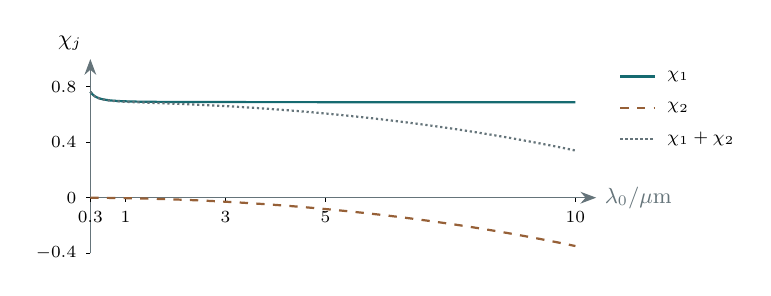
\begin{tikzpicture}[scale=.88,transform shape]
\draw[axis] (0,0.8)--(7.3,0.8) node[right] {$\lambda_0/{\rm \mu m}$};
\draw[axis] (0,0)--(0,2.8);
\node[above left] at (0,2.8) {$\chi_j$};
\draw[thin] (0.000000,0.8)--(0.000000,0.74);\node[below,font=\scriptsize] at (0.000000,0.7200000000000001) {$ 0.3 $};
\draw[thin] (0.505155,0.8)--(0.505155,0.74);\node[below,font=\scriptsize] at (0.505155,0.7200000000000001) {$ 1 $};
\draw[thin] (1.948454,0.8)--(1.948454,0.74);\node[below,font=\scriptsize] at (1.948454,0.7200000000000001) {$ 3 $};
\draw[thin] (3.391753,0.8)--(3.391753,0.74);\node[below,font=\scriptsize] at (3.391753,0.7200000000000001) {$ 5 $};
\draw[thin] (7.000000,0.8)--(7.000000,0.74);\node[below,font=\scriptsize] at (7.000000,0.7200000000000001) {$ 10 $};
\draw[thin] (0,0.000000)--(-.06,0.000000);\node[left,font=\scriptsize] at (-.08,0.000000) {$ -0.4 $};
\draw[thin] (0,0.800000)--(-.06,0.800000);\node[left,font=\scriptsize] at (-.08,0.800000) {$ 0 $};
\draw[thin] (0,1.600000)--(-.06,1.600000);\node[left,font=\scriptsize] at (-.08,1.600000) {$ 0.4 $};
\draw[thin] (0,2.400000)--(-.06,2.400000);\node[left,font=\scriptsize] at (-.08,2.400000) {$ 0.8 $};
\draw[thick,color=accent] plot coordinates {(0.0000000,2.3292660) (0.0291667,2.2927672) (0.0583333,2.2682766) (0.0875000,2.2509885) (0.1166667,2.2383031) (0.1458333,2.2287057) (0.1750000,2.2212616) (0.2041667,2.2153671) (0.2333333,2.2106174) (0.2625000,2.2067324) (0.2916667,2.2035134) (0.3208333,2.2008155) (0.3500000,2.1985317) (0.3791667,2.1965809) (0.4083333,2.1949013) (0.4375000,2.1934447) (0.4666667,2.1921731) (0.4958333,2.1910564) (0.5250000,2.1900703) (0.5541667,2.1891952) (0.5833333,2.1884151) (0.6125000,2.1877166) (0.6416667,2.1870887) (0.6708333,2.1865221) (0.7000000,2.1860092) (0.7291667,2.1855433) (0.7583333,2.1851189) (0.7875000,2.1847312) (0.8166667,2.1843761) (0.8458333,2.1840499) (0.8750000,2.1837497) (0.9041667,2.1834727) (0.9333333,2.1832166) (0.9625000,2.1829794) (0.9916667,2.1827593) (1.0208333,2.1825545) (1.0500000,2.1823639) (1.0791667,2.1821860) (1.1083333,2.1820197) (1.1375000,2.1818641) (1.1666667,2.1817183) (1.1958333,2.1815815) (1.2250000,2.1814529) (1.2541667,2.1813319) (1.2833333,2.1812179) (1.3125000,2.1811104) (1.3416667,2.1810089) (1.3708333,2.1809129) (1.4000000,2.1808221) (1.4291667,2.1807361) (1.4583333,2.1806546) (1.4875000,2.1805772) (1.5166667,2.1805037) (1.5458333,2.1804338) (1.5750000,2.1803674) (1.6041667,2.1803040) (1.6333333,2.1802437) (1.6625000,2.1801862) (1.6916667,2.1801313) (1.7208333,2.1800788) (1.7500000,2.1800287) (1.7791667,2.1799808) (1.8083333,2.1799349) (1.8375000,2.1798909) (1.8666667,2.1798488) (1.8958333,2.1798085) (1.9250000,2.1797697) (1.9541667,2.1797326) (1.9833333,2.1796969) (2.0125000,2.1796625) (2.0416667,2.1796296) (2.0708333,2.1795978) (2.1000000,2.1795673) (2.1291667,2.1795379) (2.1583333,2.1795095) (2.1875000,2.1794822) (2.2166667,2.1794559) (2.2458333,2.1794305) (2.2750000,2.1794060) (2.3041667,2.1793823) (2.3333333,2.1793595) (2.3625000,2.1793374) (2.3916667,2.1793161) (2.4208333,2.1792954) (2.4500000,2.1792755) (2.4791667,2.1792561) (2.5083333,2.1792374) (2.5375000,2.1792193) (2.5666667,2.1792018) (2.5958333,2.1791848) (2.6250000,2.1791683) (2.6541667,2.1791523) (2.6833333,2.1791368) (2.7125000,2.1791218) (2.7416667,2.1791072) (2.7708333,2.1790930) (2.8000000,2.1790793) (2.8291667,2.1790659) (2.8583333,2.1790529) (2.8875000,2.1790403) (2.9166667,2.1790280) (2.9458333,2.1790161) (2.9750000,2.1790045) (3.0041667,2.1789932) (3.0333333,2.1789822) (3.0625000,2.1789715) (3.0916667,2.1789611) (3.1208333,2.1789509) (3.1500000,2.1789411) (3.1791667,2.1789314) (3.2083333,2.1789220) (3.2375000,2.1789129) (3.2666667,2.1789040) (3.2958333,2.1788953) (3.3250000,2.1788868) (3.3541667,2.1788785) (3.3833333,2.1788704) (3.4125000,2.1788626) (3.4416667,2.1788549) (3.4708333,2.1788474) (3.5000000,2.1788400) (3.5291667,2.1788329) (3.5583333,2.1788259) (3.5875000,2.1788190) (3.6166667,2.1788123) (3.6458333,2.1788058) (3.6750000,2.1787994) (3.7041667,2.1787932) (3.7333333,2.1787871) (3.7625000,2.1787811) (3.7916667,2.1787753) (3.8208333,2.1787696) (3.8500000,2.1787640) (3.8791667,2.1787585) (3.9083333,2.1787531) (3.9375000,2.1787479) (3.9666667,2.1787427) (3.9958333,2.1787377) (4.0250000,2.1787328) (4.0541667,2.1787280) (4.0833333,2.1787232) (4.1125000,2.1787186) (4.1416667,2.1787141) (4.1708333,2.1787096) (4.2000000,2.1787053) (4.2291667,2.1787010) (4.2583333,2.1786968) (4.2875000,2.1786927) (4.3166667,2.1786886) (4.3458333,2.1786847) (4.3750000,2.1786808) (4.4041667,2.1786770) (4.4333333,2.1786733) (4.4625000,2.1786696) (4.4916667,2.1786660) (4.5208333,2.1786625) (4.5500000,2.1786590) (4.5791667,2.1786556) (4.6083333,2.1786523) (4.6375000,2.1786490) (4.6666667,2.1786458) (4.6958333,2.1786426) (4.7250000,2.1786395) (4.7541667,2.1786364) (4.7833333,2.1786334) (4.8125000,2.1786305) (4.8416667,2.1786276) (4.8708333,2.1786247) (4.9000000,2.1786219) (4.9291667,2.1786192) (4.9583333,2.1786165) (4.9875000,2.1786138) (5.0166667,2.1786112) (5.0458333,2.1786086) (5.0750000,2.1786061) (5.1041667,2.1786036) (5.1333333,2.1786011) (5.1625000,2.1785987) (5.1916667,2.1785964) (5.2208333,2.1785940) (5.2500000,2.1785917) (5.2791667,2.1785895) (5.3083333,2.1785872) (5.3375000,2.1785851) (5.3666667,2.1785829) (5.3958333,2.1785808) (5.4250000,2.1785787) (5.4541667,2.1785766) (5.4833333,2.1785746) (5.5125000,2.1785726) (5.5416667,2.1785707) (5.5708333,2.1785687) (5.6000000,2.1785668) (5.6291667,2.1785649) (5.6583333,2.1785631) (5.6875000,2.1785613) (5.7166667,2.1785595) (5.7458333,2.1785577) (5.7750000,2.1785560) (5.8041667,2.1785543) (5.8333333,2.1785526) (5.8625000,2.1785509) (5.8916667,2.1785492) (5.9208333,2.1785476) (5.9500000,2.1785460) (5.9791667,2.1785445) (6.0083333,2.1785429) (6.0375000,2.1785414) (6.0666667,2.1785399) (6.0958333,2.1785384) (6.1250000,2.1785369) (6.1541667,2.1785355) (6.1833333,2.1785340) (6.2125000,2.1785326) (6.2416667,2.1785312) (6.2708333,2.1785299) (6.3000000,2.1785285) (6.3291667,2.1785272) (6.3583333,2.1785259) (6.3875000,2.1785246) (6.4166667,2.1785233) (6.4458333,2.1785220) (6.4750000,2.1785208) (6.5041667,2.1785195) (6.5333333,2.1785183) (6.5625000,2.1785171) (6.5916667,2.1785159) (6.6208333,2.1785147) (6.6500000,2.1785136) (6.6791667,2.1785124) (6.7083333,2.1785113) (6.7375000,2.1785102) (6.7666667,2.1785091) (6.7958333,2.1785080) (6.8250000,2.1785069) (6.8541667,2.1785059) (6.8833333,2.1785048) (6.9125000,2.1785038) (6.9416667,2.1785028) (6.9708333,2.1785018) (7.0000000,2.1785008)};
\draw[thick,color=accent] (7.65,2.55)--(8.15,2.55);\node[right,font=\scriptsize] at (8.2,2.55) {$\chi_1$};
\draw[thick,dashed,color=warm] plot coordinates {(0.0000000,0.7994217) (0.0291667,0.7992554) (0.0583333,0.7990681) (0.0875000,0.7988598) (0.1166667,0.7986304) (0.1458333,0.7983801) (0.1750000,0.7981087) (0.2041667,0.7978163) (0.2333333,0.7975029) (0.2625000,0.7971685) (0.2916667,0.7968130) (0.3208333,0.7964365) (0.3500000,0.7960389) (0.3791667,0.7956203) (0.4083333,0.7951807) (0.4375000,0.7947199) (0.4666667,0.7942381) (0.4958333,0.7937353) (0.5250000,0.7932113) (0.5541667,0.7926662) (0.5833333,0.7921001) (0.6125000,0.7915128) (0.6416667,0.7909044) (0.6708333,0.7902748) (0.7000000,0.7896242) (0.7291667,0.7889523) (0.7583333,0.7882594) (0.7875000,0.7875452) (0.8166667,0.7868098) (0.8458333,0.7860533) (0.8750000,0.7852756) (0.9041667,0.7844766) (0.9333333,0.7836564) (0.9625000,0.7828149) (0.9916667,0.7819522) (1.0208333,0.7810683) (1.0500000,0.7801630) (1.0791667,0.7792364) (1.1083333,0.7782886) (1.1375000,0.7773193) (1.1666667,0.7763288) (1.1958333,0.7753169) (1.2250000,0.7742836) (1.2541667,0.7732289) (1.2833333,0.7721528) (1.3125000,0.7710553) (1.3416667,0.7699364) (1.3708333,0.7687960) (1.4000000,0.7676341) (1.4291667,0.7664507) (1.4583333,0.7652458) (1.4875000,0.7640193) (1.5166667,0.7627714) (1.5458333,0.7615018) (1.5750000,0.7602106) (1.6041667,0.7588979) (1.6333333,0.7575635) (1.6625000,0.7562074) (1.6916667,0.7548297) (1.7208333,0.7534302) (1.7500000,0.7520091) (1.7791667,0.7505662) (1.8083333,0.7491015) (1.8375000,0.7476151) (1.8666667,0.7461068) (1.8958333,0.7445767) (1.9250000,0.7430247) (1.9541667,0.7414509) (1.9833333,0.7398551) (2.0125000,0.7382374) (2.0416667,0.7365978) (2.0708333,0.7349361) (2.1000000,0.7332524) (2.1291667,0.7315467) (2.1583333,0.7298190) (2.1875000,0.7280691) (2.2166667,0.7262971) (2.2458333,0.7245030) (2.2750000,0.7226866) (2.3041667,0.7208481) (2.3333333,0.7189873) (2.3625000,0.7171043) (2.3916667,0.7151990) (2.4208333,0.7132713) (2.4500000,0.7113213) (2.4791667,0.7093488) (2.5083333,0.7073540) (2.5375000,0.7053367) (2.5666667,0.7032969) (2.5958333,0.7012346) (2.6250000,0.6991497) (2.6541667,0.6970422) (2.6833333,0.6949122) (2.7125000,0.6927594) (2.7416667,0.6905840) (2.7708333,0.6883858) (2.8000000,0.6861649) (2.8291667,0.6839212) (2.8583333,0.6816546) (2.8875000,0.6793652) (2.9166667,0.6770529) (2.9458333,0.6747176) (2.9750000,0.6723593) (3.0041667,0.6699781) (3.0333333,0.6675737) (3.0625000,0.6651463) (3.0916667,0.6626957) (3.1208333,0.6602219) (3.1500000,0.6577249) (3.1791667,0.6552047) (3.2083333,0.6526611) (3.2375000,0.6500942) (3.2666667,0.6475039) (3.2958333,0.6448902) (3.3250000,0.6422530) (3.3541667,0.6395923) (3.3833333,0.6369080) (3.4125000,0.6342001) (3.4416667,0.6314686) (3.4708333,0.6287134) (3.5000000,0.6259344) (3.5291667,0.6231317) (3.5583333,0.6203051) (3.5875000,0.6174547) (3.6166667,0.6145803) (3.6458333,0.6116819) (3.6750000,0.6087595) (3.7041667,0.6058131) (3.7333333,0.6028425) (3.7625000,0.5998478) (3.7916667,0.5968288) (3.8208333,0.5937856) (3.8500000,0.5907180) (3.8791667,0.5876261) (3.9083333,0.5845097) (3.9375000,0.5813689) (3.9666667,0.5782035) (3.9958333,0.5750136) (4.0250000,0.5717990) (4.0541667,0.5685597) (4.0833333,0.5652957) (4.1125000,0.5620069) (4.1416667,0.5586932) (4.1708333,0.5553546) (4.2000000,0.5519910) (4.2291667,0.5486024) (4.2583333,0.5451887) (4.2875000,0.5417499) (4.3166667,0.5382859) (4.3458333,0.5347966) (4.3750000,0.5312820) (4.4041667,0.5277420) (4.4333333,0.5241765) (4.4625000,0.5205856) (4.4916667,0.5169691) (4.5208333,0.5133270) (4.5500000,0.5096591) (4.5791667,0.5059656) (4.6083333,0.5022462) (4.6375000,0.4985009) (4.6666667,0.4947297) (4.6958333,0.4909324) (4.7250000,0.4871091) (4.7541667,0.4832597) (4.7833333,0.4793840) (4.8125000,0.4754820) (4.8416667,0.4715537) (4.8708333,0.4675990) (4.9000000,0.4636178) (4.9291667,0.4596101) (4.9583333,0.4555757) (4.9875000,0.4515146) (5.0166667,0.4474268) (5.0458333,0.4433121) (5.0750000,0.4391705) (5.1041667,0.4350019) (5.1333333,0.4308063) (5.1625000,0.4265835) (5.1916667,0.4223335) (5.2208333,0.4180562) (5.2500000,0.4137516) (5.2791667,0.4094195) (5.3083333,0.4050599) (5.3375000,0.4006727) (5.3666667,0.3962579) (5.3958333,0.3918153) (5.4250000,0.3873449) (5.4541667,0.3828465) (5.4833333,0.3783202) (5.5125000,0.3737657) (5.5416667,0.3691832) (5.5708333,0.3645724) (5.6000000,0.3599332) (5.6291667,0.3552657) (5.6583333,0.3505696) (5.6875000,0.3458450) (5.7166667,0.3410918) (5.7458333,0.3363097) (5.7750000,0.3314989) (5.8041667,0.3266591) (5.8333333,0.3217902) (5.8625000,0.3168923) (5.8916667,0.3119652) (5.9208333,0.3070088) (5.9500000,0.3020230) (5.9791667,0.2970078) (6.0083333,0.2919629) (6.0375000,0.2868885) (6.0666667,0.2817842) (6.0958333,0.2766502) (6.1250000,0.2714861) (6.1541667,0.2662921) (6.1833333,0.2610679) (6.2125000,0.2558134) (6.2416667,0.2505287) (6.2708333,0.2452134) (6.3000000,0.2398677) (6.3291667,0.2344913) (6.3583333,0.2290842) (6.3875000,0.2236463) (6.4166667,0.2181773) (6.4458333,0.2126774) (6.4750000,0.2071463) (6.5041667,0.2015839) (6.5333333,0.1959902) (6.5625000,0.1903650) (6.5916667,0.1847082) (6.6208333,0.1790197) (6.6500000,0.1732995) (6.6791667,0.1675473) (6.7083333,0.1617631) (6.7375000,0.1559467) (6.7666667,0.1500981) (6.7958333,0.1442172) (6.8250000,0.1383038) (6.8541667,0.1323577) (6.8833333,0.1263790) (6.9125000,0.1203675) (6.9416667,0.1143230) (6.9708333,0.1082454) (7.0000000,0.1021346)};
\draw[thick,dashed,color=warm] (7.65,2.0999999999999996)--(8.15,2.0999999999999996);\node[right,font=\scriptsize] at (8.2,2.0999999999999996) {$\chi_2$};
\draw[densely dotted,thick,color=muted] plot coordinates {(0.0000000,2.3286877) (0.0291667,2.2920226) (0.0583333,2.2673446) (0.0875000,2.2498482) (0.1166667,2.2369336) (0.1458333,2.2270858) (0.1750000,2.2193703) (0.2041667,2.2131834) (0.2333333,2.2081203) (0.2625000,2.2039009) (0.2916667,2.2003264) (0.3208333,2.1972520) (0.3500000,2.1945706) (0.3791667,2.1922013) (0.4083333,2.1900820) (0.4375000,2.1881646) (0.4666667,2.1864112) (0.4958333,2.1847916) (0.5250000,2.1832816) (0.5541667,2.1818615) (0.5833333,2.1805152) (0.6125000,2.1792294) (0.6416667,2.1779930) (0.6708333,2.1767970) (0.7000000,2.1756334) (0.7291667,2.1744957) (0.7583333,2.1733783) (0.7875000,2.1722764) (0.8166667,2.1711859) (0.8458333,2.1701032) (0.8750000,2.1690252) (0.9041667,2.1679493) (0.9333333,2.1668730) (0.9625000,2.1657944) (0.9916667,2.1647115) (1.0208333,2.1636228) (1.0500000,2.1625269) (1.0791667,2.1614224) (1.1083333,2.1603083) (1.1375000,2.1591835) (1.1666667,2.1580471) (1.1958333,2.1568984) (1.2250000,2.1557365) (1.2541667,2.1545608) (1.2833333,2.1533707) (1.3125000,2.1521657) (1.3416667,2.1509453) (1.3708333,2.1497089) (1.4000000,2.1484562) (1.4291667,2.1471868) (1.4583333,2.1459004) (1.4875000,2.1445965) (1.5166667,2.1432751) (1.5458333,2.1419356) (1.5750000,2.1405780) (1.6041667,2.1392019) (1.6333333,2.1378072) (1.6625000,2.1363936) (1.6916667,2.1349609) (1.7208333,2.1335091) (1.7500000,2.1320378) (1.7791667,2.1305469) (1.8083333,2.1290364) (1.8375000,2.1275060) (1.8666667,2.1259556) (1.8958333,2.1243851) (1.9250000,2.1227945) (1.9541667,2.1211834) (1.9833333,2.1195520) (2.0125000,2.1179000) (2.0416667,2.1162273) (2.0708333,2.1145339) (2.1000000,2.1128197) (2.1291667,2.1110846) (2.1583333,2.1093285) (2.1875000,2.1075513) (2.2166667,2.1057530) (2.2458333,2.1039335) (2.2750000,2.1020927) (2.3041667,2.1002305) (2.3333333,2.0983468) (2.3625000,2.0964417) (2.3916667,2.0945150) (2.4208333,2.0925667) (2.4500000,2.0905967) (2.4791667,2.0886050) (2.5083333,2.0865914) (2.5375000,2.0845560) (2.5666667,2.0824987) (2.5958333,2.0804194) (2.6250000,2.0783180) (2.6541667,2.0761946) (2.6833333,2.0740490) (2.7125000,2.0718812) (2.7416667,2.0696912) (2.7708333,2.0674789) (2.8000000,2.0652442) (2.8291667,2.0629871) (2.8583333,2.0607076) (2.8875000,2.0584055) (2.9166667,2.0560809) (2.9458333,2.0537337) (2.9750000,2.0513638) (3.0041667,2.0489712) (3.0333333,2.0465559) (3.0625000,2.0441178) (3.0916667,2.0416567) (3.1208333,2.0391728) (3.1500000,2.0366660) (3.1791667,2.0341361) (3.2083333,2.0315831) (3.2375000,2.0290071) (3.2666667,2.0264079) (3.2958333,2.0237855) (3.3250000,2.0211398) (3.3541667,2.0184708) (3.3833333,2.0157785) (3.4125000,2.0130627) (3.4416667,2.0103235) (3.4708333,2.0075608) (3.5000000,2.0047745) (3.5291667,2.0019646) (3.5583333,1.9991310) (3.5875000,1.9962737) (3.6166667,1.9933926) (3.6458333,1.9904877) (3.6750000,1.9875590) (3.7041667,1.9846063) (3.7333333,1.9816296) (3.7625000,1.9786289) (3.7916667,1.9756041) (3.8208333,1.9725551) (3.8500000,1.9694820) (3.8791667,1.9663846) (3.9083333,1.9632629) (3.9375000,1.9601168) (3.9666667,1.9569463) (3.9958333,1.9537513) (4.0250000,1.9505318) (4.0541667,1.9472877) (4.0833333,1.9440189) (4.1125000,1.9407255) (4.1416667,1.9374073) (4.1708333,1.9340642) (4.2000000,1.9306963) (4.2291667,1.9273034) (4.2583333,1.9238855) (4.2875000,1.9204426) (4.3166667,1.9169745) (4.3458333,1.9134813) (4.3750000,1.9099628) (4.4041667,1.9064190) (4.4333333,1.9028498) (4.4625000,1.8992552) (4.4916667,1.8956351) (4.5208333,1.8919894) (4.5500000,1.8883181) (4.5791667,1.8846212) (4.6083333,1.8808984) (4.6375000,1.8771499) (4.6666667,1.8733754) (4.6958333,1.8695750) (4.7250000,1.8657486) (4.7541667,1.8618961) (4.7833333,1.8580174) (4.8125000,1.8541125) (4.8416667,1.8501813) (4.8708333,1.8462237) (4.9000000,1.8422397) (4.9291667,1.8382292) (4.9583333,1.8341922) (4.9875000,1.8301284) (5.0166667,1.8260380) (5.0458333,1.8219207) (5.0750000,1.8177766) (5.1041667,1.8136055) (5.1333333,1.8094074) (5.1625000,1.8051822) (5.1916667,1.8009298) (5.2208333,1.7966502) (5.2500000,1.7923433) (5.2791667,1.7880090) (5.3083333,1.7836472) (5.3375000,1.7792578) (5.3666667,1.7748408) (5.3958333,1.7703961) (5.4250000,1.7659235) (5.4541667,1.7614231) (5.4833333,1.7568948) (5.5125000,1.7523384) (5.5416667,1.7477538) (5.5708333,1.7431411) (5.6000000,1.7385000) (5.6291667,1.7338306) (5.6583333,1.7291327) (5.6875000,1.7244063) (5.7166667,1.7196512) (5.7458333,1.7148674) (5.7750000,1.7100548) (5.8041667,1.7052133) (5.8333333,1.7003428) (5.8625000,1.6954432) (5.8916667,1.6905145) (5.9208333,1.6855564) (5.9500000,1.6805690) (5.9791667,1.6755522) (6.0083333,1.6705058) (6.0375000,1.6654298) (6.0666667,1.6603241) (6.0958333,1.6551885) (6.1250000,1.6500230) (6.1541667,1.6448275) (6.1833333,1.6396019) (6.2125000,1.6343460) (6.2416667,1.6290599) (6.2708333,1.6237433) (6.3000000,1.6183962) (6.3291667,1.6130185) (6.3583333,1.6076101) (6.3875000,1.6021708) (6.4166667,1.5967006) (6.4458333,1.5911994) (6.4750000,1.5856670) (6.5041667,1.5801034) (6.5333333,1.5745085) (6.5625000,1.5688821) (6.5916667,1.5632241) (6.6208333,1.5575345) (6.6500000,1.5518131) (6.6791667,1.5460597) (6.7083333,1.5402744) (6.7375000,1.5344569) (6.7666667,1.5286072) (6.7958333,1.5227252) (6.8250000,1.5168107) (6.8541667,1.5108636) (6.8833333,1.5048839) (6.9125000,1.4988713) (6.9416667,1.4928257) (6.9708333,1.4867472) (7.0000000,1.4806354)};
\draw[densely dotted,thick,color=muted] (7.65,1.65)--(8.15,1.65);\node[right,font=\scriptsize] at (8.2,1.65) {$\chi_1+\chi_2$};
\end{tikzpicture}
\figcaption{解图光5.3B\quad 电子正响应与离子负响应在透明窗口内共同作用}
\end{minipage}\end{center}
记$a_j=\lambda_j^2$，题给残数为$A_1=6.12\times10^{-15}\,\mathrm{m^2}$、$A_2=5.10\times10^{-9}\,\mathrm{m^2}$。从分式匹配得到$A_j=C_ja_j^2$，所以
\[
\frac{C_2}{C_1}
=\frac{A_2}{A_1}\left(\frac{a_1}{a_2}\right)^2
=\frac{5.10\times10^{-9}}{6.12\times10^{-15}}
\left(\frac{8.88\times10^{-15}}{1.26\times10^{-9}}\right)^2
=4.13908\times10^{-5}.
\]
强度比还包含振子数与有效电荷，一般关系为$C_2/C_1=(N_2/N_1)(q_2^2/q_1^2)(m_e/\mu)$。在已指定的等数、等电荷近似下，才简化为$C_2/C_1=m_e/\mu$。

下面由图中两个相反的回复力推导$\mu$。以$x_{\rm Ca},x_{\rm F}$表示两个离子相对各自平衡位置的位移，设$\zeta=x_{\rm Ca}-x_{\rm F}$，回复力分别为$-\kappa\zeta$、$+\kappa\zeta$，两运动方程相减，得
\[
\ddot\zeta=-\kappa\left(\frac1{m_{\mathrm{Ca}}}
+\frac1{m_{\mathrm F}}\right)\zeta,\qquad
\frac1\mu=\frac1{m_{\mathrm{Ca}}}+\frac1{m_{\mathrm F}}.
\]
因此相对坐标满足$\mu\ddot\zeta+\kappa\zeta=0$，质量为
\[
\mu=\frac{m_{\mathrm{Ca}}m_{\mathrm F}}{m_{\mathrm{Ca}}+m_{\mathrm F}}
=\frac{40\times19}{59}m_{\mathrm H}
=12.88136\,m_{\mathrm H}.
\]
这个系数来自两体相对加速度，质心运动从内部振动中分离。把$\mu=(760/59)m_{\rm H}$与光学强度比结合，有
\[
\boxed{\frac{m_{\mathrm H}}{m_e}
=\frac{59}{760}\frac{C_1}{C_2}
\simeq1.876\times10^3}.
\]
使用题给系数而在中途保留小数，结果为$m_{\rm H}/m_e=1875.58$。解图光5.3C把等数、等电荷条件下的$C_2/C_1$画成质量比的函数，观测水平线在此值相交。该交点在等数、等电荷与上述约化质量条件下确定质量比。
\begin{center}\begin{minipage}{.98\linewidth}\centering
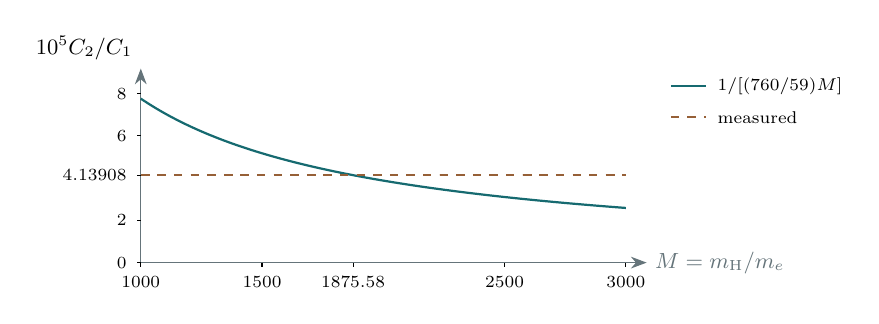
\begin{tikzpicture}[scale=.88,transform shape]
\draw[axis] (0,0.0)--(7.3,0.0) node[right] {$M=m_{\rm H}/m_e$};
\draw[axis] (0,0)--(0,2.8);
\node[above left] at (0,2.8) {$10^5 C_2/C_1$};
\draw[thin] (0.000000,0.0)--(0.000000,-0.06);\node[below,font=\scriptsize] at (0.000000,-0.08) {$ 1000 $};
\draw[thin] (1.750000,0.0)--(1.750000,-0.06);\node[below,font=\scriptsize] at (1.750000,-0.08) {$ 1500 $};
\draw[thin] (3.064530,0.0)--(3.064530,-0.06);\node[below,font=\scriptsize] at (3.064530,-0.08) {$ 1875.58 $};
\draw[thin] (5.250000,0.0)--(5.250000,-0.06);\node[below,font=\scriptsize] at (5.250000,-0.08) {$ 2500 $};
\draw[thin] (7.000000,0.0)--(7.000000,-0.06);\node[below,font=\scriptsize] at (7.000000,-0.08) {$ 3000 $};
\draw[thin] (0,0.000000)--(-.06,0.000000);\node[left,font=\scriptsize] at (-.08,0.000000) {$ 0 $};
\draw[thin] (0,0.609756)--(-.06,0.609756);\node[left,font=\scriptsize] at (-.08,0.609756) {$ 2 $};
\draw[thin] (0,1.261915)--(-.06,1.261915);\node[left,font=\scriptsize] at (-.08,1.261915) {$ 4.13908 $};
\draw[thin] (0,1.829268)--(-.06,1.829268);\node[left,font=\scriptsize] at (-.08,1.829268) {$ 6 $};
\draw[thin] (0,2.439024)--(-.06,2.439024);\node[left,font=\scriptsize] at (-.08,2.439024) {$ 8 $};
\draw[thick,color=accent] plot coordinates {(0.0000000,2.3668164) (0.0291667,2.3472560) (0.0583333,2.3280162) (0.0875000,2.3090892) (0.1166667,2.2904675) (0.1458333,2.2721438) (0.1750000,2.2541109) (0.2041667,2.2363620) (0.2333333,2.2188904) (0.2625000,2.2016897) (0.2916667,2.1847536) (0.3208333,2.1680761) (0.3500000,2.1516513) (0.3791667,2.1354735) (0.4083333,2.1195371) (0.4375000,2.1038368) (0.4666667,2.0883674) (0.4958333,2.0731239) (0.5250000,2.0581012) (0.5541667,2.0432948) (0.5833333,2.0286998) (0.6125000,2.0143119) (0.6416667,2.0001266) (0.6708333,1.9861397) (0.7000000,1.9723470) (0.7291667,1.9587446) (0.7583333,1.9453286) (0.7875000,1.9320950) (0.8166667,1.9190403) (0.8458333,1.9061609) (0.8750000,1.8934531) (0.9041667,1.8809137) (0.9333333,1.8685393) (0.9625000,1.8563266) (0.9916667,1.8442725) (1.0208333,1.8323740) (1.0500000,1.8206280) (1.0791667,1.8090317) (1.1083333,1.7975821) (1.1375000,1.7862766) (1.1666667,1.7751123) (1.1958333,1.7640868) (1.2250000,1.7531974) (1.2541667,1.7424415) (1.2833333,1.7318169) (1.3125000,1.7213210) (1.3416667,1.7109516) (1.3708333,1.7007064) (1.4000000,1.6905832) (1.4291667,1.6805797) (1.4583333,1.6706940) (1.4875000,1.6609238) (1.5166667,1.6512673) (1.5458333,1.6417224) (1.5750000,1.6322872) (1.6041667,1.6229598) (1.6333333,1.6137385) (1.6625000,1.6046213) (1.6916667,1.5956066) (1.7208333,1.5866926) (1.7500000,1.5778776) (1.7791667,1.5691601) (1.8083333,1.5605383) (1.8375000,1.5520108) (1.8666667,1.5435759) (1.8958333,1.5352323) (1.9250000,1.5269783) (1.9541667,1.5188127) (1.9833333,1.5107339) (2.0125000,1.5027406) (2.0416667,1.4948314) (2.0708333,1.4870051) (2.1000000,1.4792603) (2.1291667,1.4715957) (2.1583333,1.4640102) (2.1875000,1.4565024) (2.2166667,1.4490713) (2.2458333,1.4417156) (2.2750000,1.4344342) (2.3041667,1.4272260) (2.3333333,1.4200899) (2.3625000,1.4130247) (2.3916667,1.4060296) (2.4208333,1.3991033) (2.4500000,1.3922450) (2.4791667,1.3854535) (2.5083333,1.3787280) (2.5375000,1.3720675) (2.5666667,1.3654710) (2.5958333,1.3589377) (2.6250000,1.3524665) (2.6541667,1.3460567) (2.6833333,1.3397074) (2.7125000,1.3334177) (2.7416667,1.3271868) (2.7708333,1.3210138) (2.8000000,1.3148980) (2.8291667,1.3088386) (2.8583333,1.3028347) (2.8875000,1.2968857) (2.9166667,1.2909908) (2.9458333,1.2851492) (2.9750000,1.2793602) (3.0041667,1.2736232) (3.0333333,1.2679374) (3.0625000,1.2623021) (3.0916667,1.2567167) (3.1208333,1.2511805) (3.1500000,1.2456929) (3.1791667,1.2402532) (3.2083333,1.2348607) (3.2375000,1.2295150) (3.2666667,1.2242154) (3.2958333,1.2189613) (3.3250000,1.2137520) (3.3541667,1.2085871) (3.3833333,1.2034660) (3.4125000,1.1983881) (3.4416667,1.1933528) (3.4708333,1.1883597) (3.5000000,1.1834082) (3.5291667,1.1784978) (3.5583333,1.1736280) (3.5875000,1.1687982) (3.6166667,1.1640081) (3.6458333,1.1592570) (3.6750000,1.1545446) (3.7041667,1.1498703) (3.7333333,1.1452338) (3.7625000,1.1406344) (3.7916667,1.1360719) (3.8208333,1.1315457) (3.8500000,1.1270554) (3.8791667,1.1226007) (3.9083333,1.1181810) (3.9375000,1.1137960) (3.9666667,1.1094452) (3.9958333,1.1051283) (4.0250000,1.1008449) (4.0541667,1.0965945) (4.0833333,1.0923768) (4.1125000,1.0881915) (4.1416667,1.0840381) (4.1708333,1.0799162) (4.2000000,1.0758257) (4.2291667,1.0717659) (4.2583333,1.0677367) (4.2875000,1.0637377) (4.3166667,1.0597686) (4.3458333,1.0558289) (4.3750000,1.0519184) (4.4041667,1.0480368) (4.4333333,1.0441837) (4.4625000,1.0403589) (4.4916667,1.0365619) (4.5208333,1.0327926) (4.5500000,1.0290506) (4.5791667,1.0253356) (4.6083333,1.0216474) (4.6375000,1.0179856) (4.6666667,1.0143499) (4.6958333,1.0107401) (4.7250000,1.0071559) (4.7541667,1.0035971) (4.7833333,1.0000633) (4.8125000,0.9965543) (4.8416667,0.9930698) (4.8708333,0.9896097) (4.9000000,0.9861735) (4.9291667,0.9827611) (4.9583333,0.9793723) (4.9875000,0.9760068) (5.0166667,0.9726643) (5.0458333,0.9693446) (5.0750000,0.9660475) (5.1041667,0.9627728) (5.1333333,0.9595202) (5.1625000,0.9562895) (5.1916667,0.9530804) (5.2208333,0.9498929) (5.2500000,0.9467266) (5.2791667,0.9435813) (5.3083333,0.9404569) (5.3375000,0.9373530) (5.3666667,0.9342696) (5.3958333,0.9312065) (5.4250000,0.9281633) (5.4541667,0.9251400) (5.4833333,0.9221363) (5.5125000,0.9191520) (5.5416667,0.9161870) (5.5708333,0.9132411) (5.6000000,0.9103140) (5.6291667,0.9074057) (5.6583333,0.9045158) (5.6875000,0.9016444) (5.7166667,0.8987910) (5.7458333,0.8959557) (5.7750000,0.8931383) (5.8041667,0.8903385) (5.8333333,0.8875562) (5.8625000,0.8847912) (5.8916667,0.8820434) (5.9208333,0.8793126) (5.9500000,0.8765987) (5.9791667,0.8739015) (6.0083333,0.8712208) (6.0375000,0.8685565) (6.0666667,0.8659085) (6.0958333,0.8632765) (6.1250000,0.8606605) (6.1541667,0.8580603) (6.1833333,0.8554758) (6.2125000,0.8529068) (6.2416667,0.8503532) (6.2708333,0.8478148) (6.3000000,0.8452916) (6.3291667,0.8427833) (6.3583333,0.8402899) (6.3875000,0.8378111) (6.4166667,0.8353470) (6.4458333,0.8328973) (6.4750000,0.8304619) (6.5041667,0.8280407) (6.5333333,0.8256336) (6.5625000,0.8232405) (6.5916667,0.8208612) (6.6208333,0.8184956) (6.6500000,0.8161436) (6.6791667,0.8138051) (6.7083333,0.8114799) (6.7375000,0.8091680) (6.7666667,0.8068692) (6.7958333,0.8045835) (6.8250000,0.8023107) (6.8541667,0.8000506) (6.8833333,0.7978033) (6.9125000,0.7955685) (6.9416667,0.7933463) (6.9708333,0.7911364) (7.0000000,0.7889388)};
\draw[thick,color=accent] (7.65,2.55)--(8.15,2.55);\node[right,font=\scriptsize] at (8.2,2.55) {$1/[(760/59)M]$};
\draw[thick,dashed,color=warm] plot coordinates {(0.0000000,1.2619140) (0.0291667,1.2619140) (0.0583333,1.2619140) (0.0875000,1.2619140) (0.1166667,1.2619140) (0.1458333,1.2619140) (0.1750000,1.2619140) (0.2041667,1.2619140) (0.2333333,1.2619140) (0.2625000,1.2619140) (0.2916667,1.2619140) (0.3208333,1.2619140) (0.3500000,1.2619140) (0.3791667,1.2619140) (0.4083333,1.2619140) (0.4375000,1.2619140) (0.4666667,1.2619140) (0.4958333,1.2619140) (0.5250000,1.2619140) (0.5541667,1.2619140) (0.5833333,1.2619140) (0.6125000,1.2619140) (0.6416667,1.2619140) (0.6708333,1.2619140) (0.7000000,1.2619140) (0.7291667,1.2619140) (0.7583333,1.2619140) (0.7875000,1.2619140) (0.8166667,1.2619140) (0.8458333,1.2619140) (0.8750000,1.2619140) (0.9041667,1.2619140) (0.9333333,1.2619140) (0.9625000,1.2619140) (0.9916667,1.2619140) (1.0208333,1.2619140) (1.0500000,1.2619140) (1.0791667,1.2619140) (1.1083333,1.2619140) (1.1375000,1.2619140) (1.1666667,1.2619140) (1.1958333,1.2619140) (1.2250000,1.2619140) (1.2541667,1.2619140) (1.2833333,1.2619140) (1.3125000,1.2619140) (1.3416667,1.2619140) (1.3708333,1.2619140) (1.4000000,1.2619140) (1.4291667,1.2619140) (1.4583333,1.2619140) (1.4875000,1.2619140) (1.5166667,1.2619140) (1.5458333,1.2619140) (1.5750000,1.2619140) (1.6041667,1.2619140) (1.6333333,1.2619140) (1.6625000,1.2619140) (1.6916667,1.2619140) (1.7208333,1.2619140) (1.7500000,1.2619140) (1.7791667,1.2619140) (1.8083333,1.2619140) (1.8375000,1.2619140) (1.8666667,1.2619140) (1.8958333,1.2619140) (1.9250000,1.2619140) (1.9541667,1.2619140) (1.9833333,1.2619140) (2.0125000,1.2619140) (2.0416667,1.2619140) (2.0708333,1.2619140) (2.1000000,1.2619140) (2.1291667,1.2619140) (2.1583333,1.2619140) (2.1875000,1.2619140) (2.2166667,1.2619140) (2.2458333,1.2619140) (2.2750000,1.2619140) (2.3041667,1.2619140) (2.3333333,1.2619140) (2.3625000,1.2619140) (2.3916667,1.2619140) (2.4208333,1.2619140) (2.4500000,1.2619140) (2.4791667,1.2619140) (2.5083333,1.2619140) (2.5375000,1.2619140) (2.5666667,1.2619140) (2.5958333,1.2619140) (2.6250000,1.2619140) (2.6541667,1.2619140) (2.6833333,1.2619140) (2.7125000,1.2619140) (2.7416667,1.2619140) (2.7708333,1.2619140) (2.8000000,1.2619140) (2.8291667,1.2619140) (2.8583333,1.2619140) (2.8875000,1.2619140) (2.9166667,1.2619140) (2.9458333,1.2619140) (2.9750000,1.2619140) (3.0041667,1.2619140) (3.0333333,1.2619140) (3.0625000,1.2619140) (3.0916667,1.2619140) (3.1208333,1.2619140) (3.1500000,1.2619140) (3.1791667,1.2619140) (3.2083333,1.2619140) (3.2375000,1.2619140) (3.2666667,1.2619140) (3.2958333,1.2619140) (3.3250000,1.2619140) (3.3541667,1.2619140) (3.3833333,1.2619140) (3.4125000,1.2619140) (3.4416667,1.2619140) (3.4708333,1.2619140) (3.5000000,1.2619140) (3.5291667,1.2619140) (3.5583333,1.2619140) (3.5875000,1.2619140) (3.6166667,1.2619140) (3.6458333,1.2619140) (3.6750000,1.2619140) (3.7041667,1.2619140) (3.7333333,1.2619140) (3.7625000,1.2619140) (3.7916667,1.2619140) (3.8208333,1.2619140) (3.8500000,1.2619140) (3.8791667,1.2619140) (3.9083333,1.2619140) (3.9375000,1.2619140) (3.9666667,1.2619140) (3.9958333,1.2619140) (4.0250000,1.2619140) (4.0541667,1.2619140) (4.0833333,1.2619140) (4.1125000,1.2619140) (4.1416667,1.2619140) (4.1708333,1.2619140) (4.2000000,1.2619140) (4.2291667,1.2619140) (4.2583333,1.2619140) (4.2875000,1.2619140) (4.3166667,1.2619140) (4.3458333,1.2619140) (4.3750000,1.2619140) (4.4041667,1.2619140) (4.4333333,1.2619140) (4.4625000,1.2619140) (4.4916667,1.2619140) (4.5208333,1.2619140) (4.5500000,1.2619140) (4.5791667,1.2619140) (4.6083333,1.2619140) (4.6375000,1.2619140) (4.6666667,1.2619140) (4.6958333,1.2619140) (4.7250000,1.2619140) (4.7541667,1.2619140) (4.7833333,1.2619140) (4.8125000,1.2619140) (4.8416667,1.2619140) (4.8708333,1.2619140) (4.9000000,1.2619140) (4.9291667,1.2619140) (4.9583333,1.2619140) (4.9875000,1.2619140) (5.0166667,1.2619140) (5.0458333,1.2619140) (5.0750000,1.2619140) (5.1041667,1.2619140) (5.1333333,1.2619140) (5.1625000,1.2619140) (5.1916667,1.2619140) (5.2208333,1.2619140) (5.2500000,1.2619140) (5.2791667,1.2619140) (5.3083333,1.2619140) (5.3375000,1.2619140) (5.3666667,1.2619140) (5.3958333,1.2619140) (5.4250000,1.2619140) (5.4541667,1.2619140) (5.4833333,1.2619140) (5.5125000,1.2619140) (5.5416667,1.2619140) (5.5708333,1.2619140) (5.6000000,1.2619140) (5.6291667,1.2619140) (5.6583333,1.2619140) (5.6875000,1.2619140) (5.7166667,1.2619140) (5.7458333,1.2619140) (5.7750000,1.2619140) (5.8041667,1.2619140) (5.8333333,1.2619140) (5.8625000,1.2619140) (5.8916667,1.2619140) (5.9208333,1.2619140) (5.9500000,1.2619140) (5.9791667,1.2619140) (6.0083333,1.2619140) (6.0375000,1.2619140) (6.0666667,1.2619140) (6.0958333,1.2619140) (6.1250000,1.2619140) (6.1541667,1.2619140) (6.1833333,1.2619140) (6.2125000,1.2619140) (6.2416667,1.2619140) (6.2708333,1.2619140) (6.3000000,1.2619140) (6.3291667,1.2619140) (6.3583333,1.2619140) (6.3875000,1.2619140) (6.4166667,1.2619140) (6.4458333,1.2619140) (6.4750000,1.2619140) (6.5041667,1.2619140) (6.5333333,1.2619140) (6.5625000,1.2619140) (6.5916667,1.2619140) (6.6208333,1.2619140) (6.6500000,1.2619140) (6.6791667,1.2619140) (6.7083333,1.2619140) (6.7375000,1.2619140) (6.7666667,1.2619140) (6.7958333,1.2619140) (6.8250000,1.2619140) (6.8541667,1.2619140) (6.8833333,1.2619140) (6.9125000,1.2619140) (6.9416667,1.2619140) (6.9708333,1.2619140) (7.0000000,1.2619140)};
\draw[thick,dashed,color=warm] (7.65,2.0999999999999996)--(8.15,2.0999999999999996);\node[right,font=\scriptsize] at (8.2,2.0999999999999996) {$\mathrm{measured}$};
\end{tikzpicture}
\figcaption{解图光5.3C\quad 等数等电荷模型的质量比由残数比水平线交点确定}
\end{minipage}\end{center}
常数项也由同一次代数分解给出：
\[
C_1a_1+C_2a_2=\frac{A_1}{a_1}+\frac{A_2}{a_2}
=0.689189+4.047619=4.736808.
\]
两个振子配合真空常数1给$1+4.736808=5.736808$。题给总常数6.09相应需要
\[
\boxed{\varepsilon_b=6.09-4.736808=1.353192}.
\]
解图光5.3D在整个测量窗口比较这两个常数选择，$n^2$之间相差$.353192$。额外背景在这一有限波段内近似不随频率变，可由更远处的共振贡献；本次残数和由它们得到的强度比保持不变。
\begin{center}\begin{minipage}{.98\linewidth}\centering
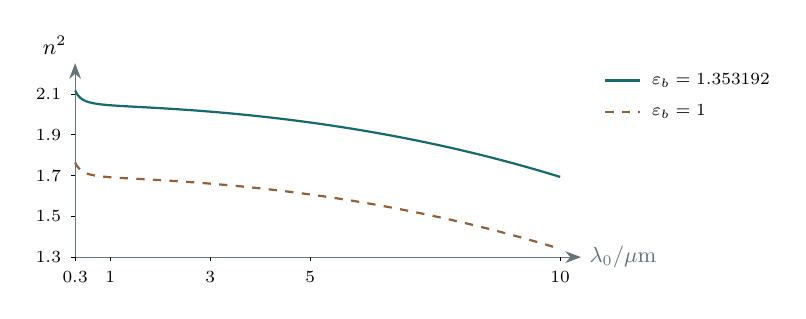
\begin{tikzpicture}[scale=.88,transform shape]
\draw[axis] (0,0)--(7.3,0) node[right] {$\lambda_0/{\rm \mu m}$};
\draw[axis] (0,0)--(0,2.8);
\node[above left] at (0,2.8) {$n^2$};
\draw[thin] (0.000000,0)--(0.000000,-0.06);\node[below,font=\scriptsize] at (0.000000,-0.08) {$ 0.3 $};
\draw[thin] (0.505155,0)--(0.505155,-0.06);\node[below,font=\scriptsize] at (0.505155,-0.08) {$ 1 $};
\draw[thin] (1.948454,0)--(1.948454,-0.06);\node[below,font=\scriptsize] at (1.948454,-0.08) {$ 3 $};
\draw[thin] (3.391753,0)--(3.391753,-0.06);\node[below,font=\scriptsize] at (3.391753,-0.08) {$ 5 $};
\draw[thin] (7.000000,0)--(7.000000,-0.06);\node[below,font=\scriptsize] at (7.000000,-0.08) {$ 10 $};
\draw[thin] (0,0.000000)--(-.06,0.000000);\node[left,font=\scriptsize] at (-.08,0.000000) {$ 1.3 $};
\draw[thin] (0,0.588235)--(-.06,0.588235);\node[left,font=\scriptsize] at (-.08,0.588235) {$ 1.5 $};
\draw[thin] (0,1.176471)--(-.06,1.176471);\node[left,font=\scriptsize] at (-.08,1.176471) {$ 1.7 $};
\draw[thin] (0,1.764706)--(-.06,1.764706);\node[left,font=\scriptsize] at (-.08,1.764706) {$ 1.9 $};
\draw[thin] (0,2.352941)--(-.06,2.352941);\node[left,font=\scriptsize] at (-.08,2.352941) {$ 2.1 $};
\draw[thick,color=accent] plot coordinates {(0.0000000,2.4045165) (0.0291667,2.3505972) (0.0583333,2.3143061) (0.0875000,2.2885761) (0.1166667,2.2695839) (0.1458333,2.2551020) (0.1750000,2.2437556) (0.2041667,2.2346572) (0.2333333,2.2272115) (0.2625000,2.2210065) (0.2916667,2.2157498) (0.3208333,2.2112287) (0.3500000,2.2072855) (0.3791667,2.2038012) (0.4083333,2.2006846) (0.4375000,2.1978649) (0.4666667,2.1952864) (0.4958333,2.1929046) (0.5250000,2.1906840) (0.5541667,2.1885956) (0.5833333,2.1866157) (0.6125000,2.1847248) (0.6416667,2.1829067) (0.6708333,2.1811478) (0.7000000,2.1794366) (0.7291667,2.1777636) (0.7583333,2.1761203) (0.7875000,2.1744999) (0.8166667,2.1728962) (0.8458333,2.1713040) (0.8750000,2.1697188) (0.9041667,2.1681365) (0.9333333,2.1665538) (0.9625000,2.1649675) (0.9916667,2.1633750) (1.0208333,2.1617740) (1.0500000,2.1601623) (1.0791667,2.1585381) (1.1083333,2.1568997) (1.1375000,2.1552456) (1.1666667,2.1535745) (1.1958333,2.1518851) (1.2250000,2.1501765) (1.2541667,2.1484476) (1.2833333,2.1466975) (1.3125000,2.1449254) (1.3416667,2.1431306) (1.3708333,2.1413124) (1.4000000,2.1394702) (1.4291667,2.1376034) (1.4583333,2.1357116) (1.4875000,2.1337942) (1.5166667,2.1318509) (1.5458333,2.1298811) (1.5750000,2.1278846) (1.6041667,2.1258609) (1.6333333,2.1238099) (1.6625000,2.1217311) (1.6916667,2.1196242) (1.7208333,2.1174891) (1.7500000,2.1153254) (1.7791667,2.1131330) (1.8083333,2.1109116) (1.8375000,2.1086611) (1.8666667,2.1063811) (1.8958333,2.1040716) (1.9250000,2.1017323) (1.9541667,2.0993632) (1.9833333,2.0969640) (2.0125000,2.0945345) (2.0416667,2.0920748) (2.0708333,2.0895845) (2.1000000,2.0870636) (2.1291667,2.0845120) (2.1583333,2.0819295) (2.1875000,2.0793160) (2.2166667,2.0766714) (2.2458333,2.0739956) (2.2750000,2.0712885) (2.3041667,2.0685500) (2.3333333,2.0657799) (2.3625000,2.0629783) (2.3916667,2.0601449) (2.4208333,2.0572798) (2.4500000,2.0543827) (2.4791667,2.0514537) (2.5083333,2.0484926) (2.5375000,2.0454993) (2.5666667,2.0424738) (2.5958333,2.0394160) (2.6250000,2.0363258) (2.6541667,2.0332031) (2.6833333,2.0300478) (2.7125000,2.0268599) (2.7416667,2.0236393) (2.7708333,2.0203859) (2.8000000,2.0170996) (2.8291667,2.0137803) (2.8583333,2.0104281) (2.8875000,2.0070427) (2.9166667,2.0036242) (2.9458333,2.0001724) (2.9750000,1.9966873) (3.0041667,1.9931688) (3.0333333,1.9896168) (3.0625000,1.9860313) (3.0916667,1.9824122) (3.1208333,1.9787594) (3.1500000,1.9750728) (3.1791667,1.9713524) (3.2083333,1.9675980) (3.2375000,1.9638097) (3.2666667,1.9599874) (3.2958333,1.9561309) (3.3250000,1.9522402) (3.3541667,1.9483152) (3.3833333,1.9443559) (3.4125000,1.9403621) (3.4416667,1.9363338) (3.4708333,1.9322710) (3.5000000,1.9281735) (3.5291667,1.9240413) (3.5583333,1.9198743) (3.5875000,1.9156724) (3.6166667,1.9114355) (3.6458333,1.9071636) (3.6750000,1.9028566) (3.7041667,1.8985144) (3.7333333,1.8941369) (3.7625000,1.8897241) (3.7916667,1.8852759) (3.8208333,1.8807921) (3.8500000,1.8762728) (3.8791667,1.8717178) (3.9083333,1.8671270) (3.9375000,1.8625005) (3.9666667,1.8578380) (3.9958333,1.8531395) (4.0250000,1.8484049) (4.0541667,1.8436341) (4.0833333,1.8388272) (4.1125000,1.8339838) (4.1416667,1.8291041) (4.1708333,1.8241878) (4.2000000,1.8192350) (4.2291667,1.8142455) (4.2583333,1.8092192) (4.2875000,1.8041560) (4.3166667,1.7990560) (4.3458333,1.7939188) (4.3750000,1.7887446) (4.4041667,1.7835331) (4.4333333,1.7782843) (4.4625000,1.7729981) (4.4916667,1.7676745) (4.5208333,1.7623132) (4.5500000,1.7569142) (4.5791667,1.7514775) (4.6083333,1.7460029) (4.6375000,1.7404903) (4.6666667,1.7349396) (4.6958333,1.7293508) (4.7250000,1.7237237) (4.7541667,1.7180582) (4.7833333,1.7123543) (4.8125000,1.7066118) (4.8416667,1.7008306) (4.8708333,1.6950107) (4.9000000,1.6891519) (4.9291667,1.6832541) (4.9583333,1.6773172) (4.9875000,1.6713411) (5.0166667,1.6653257) (5.0458333,1.6592709) (5.0750000,1.6531766) (5.1041667,1.6470427) (5.1333333,1.6408690) (5.1625000,1.6346555) (5.1916667,1.6284020) (5.2208333,1.6221085) (5.2500000,1.6157748) (5.2791667,1.6094007) (5.3083333,1.6029863) (5.3375000,1.5965314) (5.3666667,1.5900358) (5.3958333,1.5834994) (5.4250000,1.5769222) (5.4541667,1.5703039) (5.4833333,1.5636446) (5.5125000,1.5569440) (5.5416667,1.5502020) (5.5708333,1.5434185) (5.6000000,1.5365935) (5.6291667,1.5297267) (5.6583333,1.5228180) (5.6875000,1.5158674) (5.7166667,1.5088746) (5.7458333,1.5018396) (5.7750000,1.4947623) (5.8041667,1.4876424) (5.8333333,1.4804799) (5.8625000,1.4732746) (5.8916667,1.4660264) (5.9208333,1.4587352) (5.9500000,1.4514008) (5.9791667,1.4440232) (6.0083333,1.4366020) (6.0375000,1.4291373) (6.0666667,1.4216289) (6.0958333,1.4140765) (6.1250000,1.4064802) (6.1541667,1.3988398) (6.1833333,1.3911550) (6.2125000,1.3834258) (6.2416667,1.3756521) (6.2708333,1.3678336) (6.3000000,1.3599702) (6.3291667,1.3520618) (6.3583333,1.3441082) (6.3875000,1.3361093) (6.4166667,1.3280649) (6.4458333,1.3199749) (6.4750000,1.3118391) (6.5041667,1.3036573) (6.5333333,1.2954295) (6.5625000,1.2871553) (6.5916667,1.2788348) (6.6208333,1.2704677) (6.6500000,1.2620538) (6.6791667,1.2535930) (6.7083333,1.2450852) (6.7375000,1.2365301) (6.7666667,1.2279276) (6.7958333,1.2192776) (6.8250000,1.2105798) (6.8541667,1.2018341) (6.8833333,1.1930403) (6.9125000,1.1841982) (6.9416667,1.1753078) (6.9708333,1.1663687) (7.0000000,1.1573808)};
\draw[thick,color=accent] (7.65,2.55)--(8.15,2.55);\node[right,font=\scriptsize] at (8.2,2.55) {$\varepsilon_b=1.353192$};
\draw[thick,dashed,color=warm] plot coordinates {(0.0000000,1.3657172) (0.0291667,1.3117979) (0.0583333,1.2755068) (0.0875000,1.2497768) (0.1166667,1.2307846) (0.1458333,1.2163027) (0.1750000,1.2049563) (0.2041667,1.1958579) (0.2333333,1.1884122) (0.2625000,1.1822072) (0.2916667,1.1769505) (0.3208333,1.1724294) (0.3500000,1.1684862) (0.3791667,1.1650019) (0.4083333,1.1618853) (0.4375000,1.1590656) (0.4666667,1.1564871) (0.4958333,1.1541053) (0.5250000,1.1518847) (0.5541667,1.1497963) (0.5833333,1.1478164) (0.6125000,1.1459255) (0.6416667,1.1441074) (0.6708333,1.1423485) (0.7000000,1.1406373) (0.7291667,1.1389642) (0.7583333,1.1373210) (0.7875000,1.1357006) (0.8166667,1.1340969) (0.8458333,1.1325047) (0.8750000,1.1309195) (0.9041667,1.1293372) (0.9333333,1.1277544) (0.9625000,1.1261682) (0.9916667,1.1245757) (1.0208333,1.1229747) (1.0500000,1.1213630) (1.0791667,1.1197388) (1.1083333,1.1181004) (1.1375000,1.1164463) (1.1666667,1.1147752) (1.1958333,1.1130858) (1.2250000,1.1113772) (1.2541667,1.1096483) (1.2833333,1.1078981) (1.3125000,1.1061261) (1.3416667,1.1043313) (1.3708333,1.1025131) (1.4000000,1.1006709) (1.4291667,1.0988041) (1.4583333,1.0969123) (1.4875000,1.0949949) (1.5166667,1.0930516) (1.5458333,1.0910818) (1.5750000,1.0890853) (1.6041667,1.0870616) (1.6333333,1.0850106) (1.6625000,1.0829317) (1.6916667,1.0808249) (1.7208333,1.0786898) (1.7500000,1.0765261) (1.7791667,1.0743337) (1.8083333,1.0721123) (1.8375000,1.0698618) (1.8666667,1.0675818) (1.8958333,1.0652723) (1.9250000,1.0629330) (1.9541667,1.0605639) (1.9833333,1.0581647) (2.0125000,1.0557352) (2.0416667,1.0532755) (2.0708333,1.0507852) (2.1000000,1.0482643) (2.1291667,1.0457127) (2.1583333,1.0431302) (2.1875000,1.0405167) (2.2166667,1.0378721) (2.2458333,1.0351963) (2.2750000,1.0324892) (2.3041667,1.0297507) (2.3333333,1.0269806) (2.3625000,1.0241790) (2.3916667,1.0213456) (2.4208333,1.0184805) (2.4500000,1.0155834) (2.4791667,1.0126544) (2.5083333,1.0096933) (2.5375000,1.0067000) (2.5666667,1.0036745) (2.5958333,1.0006167) (2.6250000,0.9975265) (2.6541667,0.9944038) (2.6833333,0.9912485) (2.7125000,0.9880606) (2.7416667,0.9848400) (2.7708333,0.9815866) (2.8000000,0.9783003) (2.8291667,0.9749810) (2.8583333,0.9716288) (2.8875000,0.9682434) (2.9166667,0.9648249) (2.9458333,0.9613731) (2.9750000,0.9578880) (3.0041667,0.9543695) (3.0333333,0.9508175) (3.0625000,0.9472320) (3.0916667,0.9436129) (3.1208333,0.9399600) (3.1500000,0.9362735) (3.1791667,0.9325531) (3.2083333,0.9287987) (3.2375000,0.9250104) (3.2666667,0.9211881) (3.2958333,0.9173316) (3.3250000,0.9134409) (3.3541667,0.9095159) (3.3833333,0.9055566) (3.4125000,0.9015628) (3.4416667,0.8975345) (3.4708333,0.8934717) (3.5000000,0.8893742) (3.5291667,0.8852420) (3.5583333,0.8810750) (3.5875000,0.8768731) (3.6166667,0.8726362) (3.6458333,0.8683643) (3.6750000,0.8640573) (3.7041667,0.8597151) (3.7333333,0.8553376) (3.7625000,0.8509248) (3.7916667,0.8464766) (3.8208333,0.8419928) (3.8500000,0.8374735) (3.8791667,0.8329185) (3.9083333,0.8283277) (3.9375000,0.8237012) (3.9666667,0.8190387) (3.9958333,0.8143402) (4.0250000,0.8096056) (4.0541667,0.8048348) (4.0833333,0.8000278) (4.1125000,0.7951845) (4.1416667,0.7903048) (4.1708333,0.7853885) (4.2000000,0.7804357) (4.2291667,0.7754462) (4.2583333,0.7704199) (4.2875000,0.7653567) (4.3166667,0.7602567) (4.3458333,0.7551195) (4.3750000,0.7499453) (4.4041667,0.7447338) (4.4333333,0.7394850) (4.4625000,0.7341988) (4.4916667,0.7288752) (4.5208333,0.7235139) (4.5500000,0.7181149) (4.5791667,0.7126782) (4.6083333,0.7072036) (4.6375000,0.7016910) (4.6666667,0.6961403) (4.6958333,0.6905515) (4.7250000,0.6849244) (4.7541667,0.6792589) (4.7833333,0.6735550) (4.8125000,0.6678125) (4.8416667,0.6620313) (4.8708333,0.6562114) (4.9000000,0.6503526) (4.9291667,0.6444548) (4.9583333,0.6385179) (4.9875000,0.6325418) (5.0166667,0.6265264) (5.0458333,0.6204716) (5.0750000,0.6143773) (5.1041667,0.6082434) (5.1333333,0.6020697) (5.1625000,0.5958562) (5.1916667,0.5896027) (5.2208333,0.5833092) (5.2500000,0.5769755) (5.2791667,0.5706014) (5.3083333,0.5641870) (5.3375000,0.5577321) (5.3666667,0.5512365) (5.3958333,0.5447001) (5.4250000,0.5381229) (5.4541667,0.5315046) (5.4833333,0.5248453) (5.5125000,0.5181447) (5.5416667,0.5114027) (5.5708333,0.5046192) (5.6000000,0.4977942) (5.6291667,0.4909274) (5.6583333,0.4840187) (5.6875000,0.4770681) (5.7166667,0.4700753) (5.7458333,0.4630403) (5.7750000,0.4559630) (5.8041667,0.4488431) (5.8333333,0.4416806) (5.8625000,0.4344753) (5.8916667,0.4272271) (5.9208333,0.4199359) (5.9500000,0.4126015) (5.9791667,0.4052238) (6.0083333,0.3978027) (6.0375000,0.3903380) (6.0666667,0.3828296) (6.0958333,0.3752772) (6.1250000,0.3676809) (6.1541667,0.3600405) (6.1833333,0.3523557) (6.2125000,0.3446265) (6.2416667,0.3368528) (6.2708333,0.3290343) (6.3000000,0.3211709) (6.3291667,0.3132625) (6.3583333,0.3053089) (6.3875000,0.2973100) (6.4166667,0.2892656) (6.4458333,0.2811756) (6.4750000,0.2730398) (6.5041667,0.2648580) (6.5333333,0.2566301) (6.5625000,0.2483560) (6.5916667,0.2400355) (6.6208333,0.2316684) (6.6500000,0.2232545) (6.6791667,0.2147937) (6.7083333,0.2062859) (6.7375000,0.1977308) (6.7666667,0.1891283) (6.7958333,0.1804782) (6.8250000,0.1717805) (6.8541667,0.1630347) (6.8833333,0.1542410) (6.9125000,0.1453989) (6.9416667,0.1365085) (6.9708333,0.1275694) (7.0000000,0.1185815)};
\draw[thick,dashed,color=warm] (7.65,2.0999999999999996)--(8.15,2.0999999999999996);\node[right,font=\scriptsize] at (8.2,2.0999999999999996) {$\varepsilon_b=1$};
\end{tikzpicture}
\figcaption{解图光5.3D\quad 同一极点残数下背景使折射率平方整体平移0.353192}
\end{minipage}\end{center}
质量比是上述有效模型下的估计。实际晶体的离子集体振动和有效电荷可以用更多模态及相应权重表示，其他电子共振也进入完整高频响应；当前透明窗口内的折射率由这两个极点及常数背景共同描述。


\Needspace{8\baselineskip}

\pdfbookmark[3]{关键洞察}{q3-h5}

\subsection*{关键洞察}

两个极点给出两种主要振动尺度，残数还含计数和电荷。保持同一组极点残数时，近似常数背景补足总折射率，却不改变本次强度比。质量估计的条件与完整透明窗口色散的匹配因此可以分别写清。

\Needspace{8\baselineskip}

\pdfbookmark[3]{易错点}{q3-h6}

\subsection*{易错点}

\begin{itemize}
\item 残数为$A_j=C_j\lambda_j^4$，比较质量前先消去波长四次方。
\item 离子振动用$\mu^{-1}=m_{\rm Ca}^{-1}+m_{\rm F}^{-1}$，两个质量之和描述质心平移。
\item 两振子常数加1给5.736808，题给6.09由额外$.353192$背景补足。
\item 强度比保留$N_2q_2^2/(N_1q_1^2)$，等数、等电荷代入后才成为质量倒数比。
\end{itemize}

\Needspace{8\baselineskip}

\pdfbookmark[3]{课堂讲解建议}{q3-h7}

\subsection*{课堂讲解建议}

让学生先从两个分母给出波长，再把每个残数写成$C_j\lambda_j^4$。两体质量方程相减后，讨论为何出现倒数质量之和；在C图代入质量比并读观测交点。最后亲算两个振子的常数贡献，与6.09作差，用D图说明背景项的作用。变式分别改变电荷、计数和同位素质量，观察哪一条匹配关系随之改变。

\Needspace{8\baselineskip}

\pdfbookmark[3]{变式训练}{q3-h8}

\subsection*{变式训练}

\begin{enumerate}
\item \textbf{离子有效电荷加倍。}保留同样极点残数和等数假设，若$|q_2|=2|q_1|$，重新求质量比。

一般强度比为$R=C_2/C_1=(q_2/q_1)^2m_e/\mu$，因此$R=4m_e/\mu$。仍取$\mu=(760/59)m_{\rm H}$，得$m_{\rm H}/m_e=4(59/760)/R=7502.31$，为等电荷估计的4倍。变图光5.3V1随电荷比$g=|q_2/q_1|$画质量推断$M(g)=g^2M(1)$，显示同一光学残数对应的电荷—质量组合。
\begin{center}\begin{minipage}{.98\linewidth}\centering
\begin{tikzpicture}[scale=.88,transform shape]
\draw[axis] (0,0.0)--(7.3,0.0) node[right] {$|q_2/q_1|$};
\draw[axis] (0,0)--(0,2.8);
\node[above left] at (0,2.8) {$M=m_{\rm H}/m_e$};
\draw[thin] (0.000000,0.0)--(0.000000,-0.06);\node[below,font=\scriptsize] at (0.000000,-0.08) {$ 0.5 $};
\draw[thin] (2.333333,0.0)--(2.333333,-0.06);\node[below,font=\scriptsize] at (2.333333,-0.08) {$ 1 $};
\draw[thin] (4.666667,0.0)--(4.666667,-0.06);\node[below,font=\scriptsize] at (4.666667,-0.08) {$ 1.5 $};
\draw[thin] (7.000000,0.0)--(7.000000,-0.06);\node[below,font=\scriptsize] at (7.000000,-0.08) {$ 2 $};
\draw[thin] (0,0.000000)--(-.06,0.000000);\node[left,font=\scriptsize] at (-.08,0.000000) {$ 0 $};
\draw[thin] (0,0.625000)--(-.06,0.625000);\node[left,font=\scriptsize] at (-.08,0.625000) {$ 2000 $};
\draw[thin] (0,1.250000)--(-.06,1.250000);\node[left,font=\scriptsize] at (-.08,1.250000) {$ 4000 $};
\draw[thin] (0,1.875000)--(-.06,1.875000);\node[left,font=\scriptsize] at (-.08,1.875000) {$ 6000 $};
\draw[thin] (0,2.500000)--(-.06,2.500000);\node[left,font=\scriptsize] at (-.08,2.500000) {$ 8000 $};
\draw[thick,color=accent] plot coordinates {(0.0000000,0.1465294) (0.0291667,0.1502156) (0.0583333,0.1539475) (0.0875000,0.1577252) (0.1166667,0.1615487) (0.1458333,0.1654180) (0.1750000,0.1693331) (0.2041667,0.1732939) (0.2333333,0.1773006) (0.2625000,0.1813531) (0.2916667,0.1854513) (0.3208333,0.1895953) (0.3500000,0.1937852) (0.3791667,0.1980208) (0.4083333,0.2023022) (0.4375000,0.2066294) (0.4666667,0.2110024) (0.4958333,0.2154212) (0.5250000,0.2198857) (0.5541667,0.2243961) (0.5833333,0.2289522) (0.6125000,0.2335542) (0.6416667,0.2382019) (0.6708333,0.2428954) (0.7000000,0.2476347) (0.7291667,0.2524198) (0.7583333,0.2572507) (0.7875000,0.2621274) (0.8166667,0.2670499) (0.8458333,0.2720181) (0.8750000,0.2770322) (0.9041667,0.2820920) (0.9333333,0.2871977) (0.9625000,0.2923491) (0.9916667,0.2975463) (1.0208333,0.3027893) (1.0500000,0.3080781) (1.0791667,0.3134127) (1.1083333,0.3187931) (1.1375000,0.3242193) (1.1666667,0.3296912) (1.1958333,0.3352090) (1.2250000,0.3407725) (1.2541667,0.3463818) (1.2833333,0.3520370) (1.3125000,0.3577379) (1.3416667,0.3634846) (1.3708333,0.3692771) (1.4000000,0.3751153) (1.4291667,0.3809994) (1.4583333,0.3869293) (1.4875000,0.3929049) (1.5166667,0.3989264) (1.5458333,0.4049936) (1.5750000,0.4111066) (1.6041667,0.4172654) (1.6333333,0.4234700) (1.6625000,0.4297204) (1.6916667,0.4360166) (1.7208333,0.4423586) (1.7500000,0.4487464) (1.7791667,0.4551799) (1.8083333,0.4616593) (1.8375000,0.4681844) (1.8666667,0.4747553) (1.8958333,0.4813721) (1.9250000,0.4880346) (1.9541667,0.4947429) (1.9833333,0.5014970) (2.0125000,0.5082968) (2.0416667,0.5151425) (2.0708333,0.5220340) (2.1000000,0.5289712) (2.1291667,0.5359543) (2.1583333,0.5429831) (2.1875000,0.5500577) (2.2166667,0.5571782) (2.2458333,0.5643444) (2.2750000,0.5715564) (2.3041667,0.5788141) (2.3333333,0.5861177) (2.3625000,0.5934671) (2.3916667,0.6008622) (2.4208333,0.6083032) (2.4500000,0.6157899) (2.4791667,0.6233224) (2.5083333,0.6309008) (2.5375000,0.6385249) (2.5666667,0.6461948) (2.5958333,0.6539105) (2.6250000,0.6616719) (2.6541667,0.6694792) (2.6833333,0.6773323) (2.7125000,0.6852311) (2.7416667,0.6931758) (2.7708333,0.7011662) (2.8000000,0.7092024) (2.8291667,0.7172844) (2.8583333,0.7254122) (2.8875000,0.7335858) (2.9166667,0.7418052) (2.9458333,0.7500704) (2.9750000,0.7583814) (3.0041667,0.7667381) (3.0333333,0.7751407) (3.0625000,0.7835890) (3.0916667,0.7920831) (3.1208333,0.8006231) (3.1500000,0.8092088) (3.1791667,0.8178403) (3.2083333,0.8265176) (3.2375000,0.8352406) (3.2666667,0.8440095) (3.2958333,0.8528242) (3.3250000,0.8616846) (3.3541667,0.8705909) (3.3833333,0.8795429) (3.4125000,0.8885407) (3.4416667,0.8975843) (3.4708333,0.9066737) (3.5000000,0.9158089) (3.5291667,0.9249899) (3.5583333,0.9342167) (3.5875000,0.9434893) (3.6166667,0.9528076) (3.6458333,0.9621718) (3.6750000,0.9715817) (3.7041667,0.9810374) (3.7333333,0.9905389) (3.7625000,1.0000862) (3.7916667,1.0096793) (3.8208333,1.0193182) (3.8500000,1.0290029) (3.8791667,1.0387334) (3.9083333,1.0485096) (3.9375000,1.0583317) (3.9666667,1.0681995) (3.9958333,1.0781132) (4.0250000,1.0880726) (4.0541667,1.0980778) (4.0833333,1.1081288) (4.1125000,1.1182256) (4.1416667,1.1283682) (4.1708333,1.1385566) (4.2000000,1.1487907) (4.2291667,1.1590707) (4.2583333,1.1693964) (4.2875000,1.1797680) (4.3166667,1.1901853) (4.3458333,1.2006484) (4.3750000,1.2111573) (4.4041667,1.2217120) (4.4333333,1.2323125) (4.4625000,1.2429588) (4.4916667,1.2536508) (4.5208333,1.2643887) (4.5500000,1.2751723) (4.5791667,1.2860018) (4.6083333,1.2968770) (4.6375000,1.3077980) (4.6666667,1.3187649) (4.6958333,1.3297775) (4.7250000,1.3408358) (4.7541667,1.3519400) (4.7833333,1.3630900) (4.8125000,1.3742858) (4.8416667,1.3855273) (4.8708333,1.3968147) (4.9000000,1.4081478) (4.9291667,1.4195267) (4.9583333,1.4309514) (4.9875000,1.4424220) (5.0166667,1.4539382) (5.0458333,1.4655003) (5.0750000,1.4771082) (5.1041667,1.4887619) (5.1333333,1.5004613) (5.1625000,1.5122066) (5.1916667,1.5239976) (5.2208333,1.5358345) (5.2500000,1.5477171) (5.2791667,1.5596455) (5.3083333,1.5716197) (5.3375000,1.5836397) (5.3666667,1.5957055) (5.3958333,1.6078170) (5.4250000,1.6199744) (5.4541667,1.6321776) (5.4833333,1.6444265) (5.5125000,1.6567212) (5.5416667,1.6690618) (5.5708333,1.6814481) (5.6000000,1.6938802) (5.6291667,1.7063581) (5.6583333,1.7188818) (5.6875000,1.7314512) (5.7166667,1.7440665) (5.7458333,1.7567276) (5.7750000,1.7694344) (5.8041667,1.7821871) (5.8333333,1.7949855) (5.8625000,1.8078297) (5.8916667,1.8207197) (5.9208333,1.8336555) (5.9500000,1.8466371) (5.9791667,1.8596645) (6.0083333,1.8727377) (6.0375000,1.8858566) (6.0666667,1.8990214) (6.0958333,1.9122319) (6.1250000,1.9254883) (6.1541667,1.9387904) (6.1833333,1.9521383) (6.2125000,1.9655320) (6.2416667,1.9789715) (6.2708333,1.9924568) (6.3000000,2.0059879) (6.3291667,2.0195647) (6.3583333,2.0331874) (6.3875000,2.0468558) (6.4166667,2.0605701) (6.4458333,2.0743301) (6.4750000,2.0881359) (6.5041667,2.1019875) (6.5333333,2.1158849) (6.5625000,2.1298281) (6.5916667,2.1438171) (6.6208333,2.1578519) (6.6500000,2.1719324) (6.6791667,2.1860588) (6.7083333,2.2002309) (6.7375000,2.2144489) (6.7666667,2.2287126) (6.7958333,2.2430221) (6.8250000,2.2573774) (6.8541667,2.2717785) (6.8833333,2.2862254) (6.9125000,2.3007181) (6.9416667,2.3152565) (6.9708333,2.3298408) (7.0000000,2.3444708)};
\end{tikzpicture}
\figcaption{变图光5.3V1\quad 固定残数比时质量估计随有效电荷比平方变化}
\end{minipage}\end{center}
\item \textbf{离子振子数只有一半。}令$N_2=N_1/2$且有效电荷相等，其他测量数据相同，求质量比。

由$R=(N_2/N_1)m_e/\mu$得到$R=m_e/(2\mu)$。因此$m_{\rm H}/m_e=(1/2)(59/760)/R=937.788$。变图光5.3V2画$M(\sigma)=\sigma M(1)$，其中$\sigma=N_2/N_1$；振子数和质量通过这一组合共同影响强度，光学数据固定组合后再由计数假设确定质量。
\begin{center}\begin{minipage}{.98\linewidth}\centering
\begin{tikzpicture}[scale=.88,transform shape]
\draw[axis] (0,0.0)--(7.3,0.0) node[right] {$N_2/N_1$};
\draw[axis] (0,0)--(0,2.8);
\node[above left] at (0,2.8) {$M=m_{\rm H}/m_e$};
\draw[thin] (0.000000,0.0)--(0.000000,-0.06);\node[below,font=\scriptsize] at (0.000000,-0.08) {$ 0.25 $};
\draw[thin] (1.400000,0.0)--(1.400000,-0.06);\node[below,font=\scriptsize] at (1.400000,-0.08) {$ 0.5 $};
\draw[thin] (4.200000,0.0)--(4.200000,-0.06);\node[below,font=\scriptsize] at (4.200000,-0.08) {$ 1 $};
\draw[thin] (7.000000,0.0)--(7.000000,-0.06);\node[below,font=\scriptsize] at (7.000000,-0.08) {$ 1.5 $};
\draw[thin] (0,0.000000)--(-.06,0.000000);\node[left,font=\scriptsize] at (-.08,0.000000) {$ 0 $};
\draw[thin] (0,0.781490)--(-.06,0.781490);\node[left,font=\scriptsize] at (-.08,0.781490) {$ 937.788 $};
\draw[thin] (0,1.562983)--(-.06,1.562983);\node[left,font=\scriptsize] at (-.08,1.562983) {$ 1875.58 $};
\draw[thin] (0,2.333333)--(-.06,2.333333);\node[left,font=\scriptsize] at (-.08,2.333333) {$ 2800 $};
\draw[thick,color=accent] plot coordinates {(0.0000000,0.3907451) (0.0291667,0.3988857) (0.0583333,0.4070262) (0.0875000,0.4151667) (0.1166667,0.4233072) (0.1458333,0.4314478) (0.1750000,0.4395883) (0.2041667,0.4477288) (0.2333333,0.4558693) (0.2625000,0.4640099) (0.2916667,0.4721504) (0.3208333,0.4802909) (0.3500000,0.4884314) (0.3791667,0.4965720) (0.4083333,0.5047125) (0.4375000,0.5128530) (0.4666667,0.5209935) (0.4958333,0.5291340) (0.5250000,0.5372746) (0.5541667,0.5454151) (0.5833333,0.5535556) (0.6125000,0.5616961) (0.6416667,0.5698367) (0.6708333,0.5779772) (0.7000000,0.5861177) (0.7291667,0.5942582) (0.7583333,0.6023988) (0.7875000,0.6105393) (0.8166667,0.6186798) (0.8458333,0.6268203) (0.8750000,0.6349609) (0.9041667,0.6431014) (0.9333333,0.6512419) (0.9625000,0.6593824) (0.9916667,0.6675230) (1.0208333,0.6756635) (1.0500000,0.6838040) (1.0791667,0.6919445) (1.1083333,0.7000850) (1.1375000,0.7082256) (1.1666667,0.7163661) (1.1958333,0.7245066) (1.2250000,0.7326471) (1.2541667,0.7407877) (1.2833333,0.7489282) (1.3125000,0.7570687) (1.3416667,0.7652092) (1.3708333,0.7733498) (1.4000000,0.7814903) (1.4291667,0.7896308) (1.4583333,0.7977713) (1.4875000,0.8059119) (1.5166667,0.8140524) (1.5458333,0.8221929) (1.5750000,0.8303334) (1.6041667,0.8384739) (1.6333333,0.8466145) (1.6625000,0.8547550) (1.6916667,0.8628955) (1.7208333,0.8710360) (1.7500000,0.8791766) (1.7791667,0.8873171) (1.8083333,0.8954576) (1.8375000,0.9035981) (1.8666667,0.9117387) (1.8958333,0.9198792) (1.9250000,0.9280197) (1.9541667,0.9361602) (1.9833333,0.9443008) (2.0125000,0.9524413) (2.0416667,0.9605818) (2.0708333,0.9687223) (2.1000000,0.9768629) (2.1291667,0.9850034) (2.1583333,0.9931439) (2.1875000,1.0012844) (2.2166667,1.0094249) (2.2458333,1.0175655) (2.2750000,1.0257060) (2.3041667,1.0338465) (2.3333333,1.0419870) (2.3625000,1.0501276) (2.3916667,1.0582681) (2.4208333,1.0664086) (2.4500000,1.0745491) (2.4791667,1.0826897) (2.5083333,1.0908302) (2.5375000,1.0989707) (2.5666667,1.1071112) (2.5958333,1.1152518) (2.6250000,1.1233923) (2.6541667,1.1315328) (2.6833333,1.1396733) (2.7125000,1.1478139) (2.7416667,1.1559544) (2.7708333,1.1640949) (2.8000000,1.1722354) (2.8291667,1.1803759) (2.8583333,1.1885165) (2.8875000,1.1966570) (2.9166667,1.2047975) (2.9458333,1.2129380) (2.9750000,1.2210786) (3.0041667,1.2292191) (3.0333333,1.2373596) (3.0625000,1.2455001) (3.0916667,1.2536407) (3.1208333,1.2617812) (3.1500000,1.2699217) (3.1791667,1.2780622) (3.2083333,1.2862028) (3.2375000,1.2943433) (3.2666667,1.3024838) (3.2958333,1.3106243) (3.3250000,1.3187649) (3.3541667,1.3269054) (3.3833333,1.3350459) (3.4125000,1.3431864) (3.4416667,1.3513269) (3.4708333,1.3594675) (3.5000000,1.3676080) (3.5291667,1.3757485) (3.5583333,1.3838890) (3.5875000,1.3920296) (3.6166667,1.4001701) (3.6458333,1.4083106) (3.6750000,1.4164511) (3.7041667,1.4245917) (3.7333333,1.4327322) (3.7625000,1.4408727) (3.7916667,1.4490132) (3.8208333,1.4571538) (3.8500000,1.4652943) (3.8791667,1.4734348) (3.9083333,1.4815753) (3.9375000,1.4897159) (3.9666667,1.4978564) (3.9958333,1.5059969) (4.0250000,1.5141374) (4.0541667,1.5222779) (4.0833333,1.5304185) (4.1125000,1.5385590) (4.1416667,1.5466995) (4.1708333,1.5548400) (4.2000000,1.5629806) (4.2291667,1.5711211) (4.2583333,1.5792616) (4.2875000,1.5874021) (4.3166667,1.5955427) (4.3458333,1.6036832) (4.3750000,1.6118237) (4.4041667,1.6199642) (4.4333333,1.6281048) (4.4625000,1.6362453) (4.4916667,1.6443858) (4.5208333,1.6525263) (4.5500000,1.6606669) (4.5791667,1.6688074) (4.6083333,1.6769479) (4.6375000,1.6850884) (4.6666667,1.6932289) (4.6958333,1.7013695) (4.7250000,1.7095100) (4.7541667,1.7176505) (4.7833333,1.7257910) (4.8125000,1.7339316) (4.8416667,1.7420721) (4.8708333,1.7502126) (4.9000000,1.7583531) (4.9291667,1.7664937) (4.9583333,1.7746342) (4.9875000,1.7827747) (5.0166667,1.7909152) (5.0458333,1.7990558) (5.0750000,1.8071963) (5.1041667,1.8153368) (5.1333333,1.8234773) (5.1625000,1.8316179) (5.1916667,1.8397584) (5.2208333,1.8478989) (5.2500000,1.8560394) (5.2791667,1.8641799) (5.3083333,1.8723205) (5.3375000,1.8804610) (5.3666667,1.8886015) (5.3958333,1.8967420) (5.4250000,1.9048826) (5.4541667,1.9130231) (5.4833333,1.9211636) (5.5125000,1.9293041) (5.5416667,1.9374447) (5.5708333,1.9455852) (5.6000000,1.9537257) (5.6291667,1.9618662) (5.6583333,1.9700068) (5.6875000,1.9781473) (5.7166667,1.9862878) (5.7458333,1.9944283) (5.7750000,2.0025689) (5.8041667,2.0107094) (5.8333333,2.0188499) (5.8625000,2.0269904) (5.8916667,2.0351309) (5.9208333,2.0432715) (5.9500000,2.0514120) (5.9791667,2.0595525) (6.0083333,2.0676930) (6.0375000,2.0758336) (6.0666667,2.0839741) (6.0958333,2.0921146) (6.1250000,2.1002551) (6.1541667,2.1083957) (6.1833333,2.1165362) (6.2125000,2.1246767) (6.2416667,2.1328172) (6.2708333,2.1409578) (6.3000000,2.1490983) (6.3291667,2.1572388) (6.3583333,2.1653793) (6.3875000,2.1735198) (6.4166667,2.1816604) (6.4458333,2.1898009) (6.4750000,2.1979414) (6.5041667,2.2060819) (6.5333333,2.2142225) (6.5625000,2.2223630) (6.5916667,2.2305035) (6.6208333,2.2386440) (6.6500000,2.2467846) (6.6791667,2.2549251) (6.7083333,2.2630656) (6.7375000,2.2712061) (6.7666667,2.2793467) (6.7958333,2.2874872) (6.8250000,2.2956277) (6.8541667,2.3037682) (6.8833333,2.3119088) (6.9125000,2.3200493) (6.9416667,2.3281898) (6.9708333,2.3363303) (7.0000000,2.3444708)};
\end{tikzpicture}
\figcaption{变图光5.3V2\quad 指定离子振子计数后由同一强度比求质量}
\end{minipage}\end{center}
\item \textbf{两离子质量同比例改变。}把Ca、F两有效质量都乘$s$，回复力常数$\kappa$、数密度和有效电荷保持。求离子共振波长、$C_2$与极点残数$A_2$的变化。

约化质量乘$s$，由$\omega_2^2=\kappa/\mu$得$\omega'_2=\omega_2/\sqrt s$，所以$\lambda'_2=\sqrt s\lambda_2$。同时$C'_2=C_2/s$，而$A'_2=C'_2\lambda_2'^4=sA_2$。变图光5.3V3显示波长按平方根变化；例如$s=2$时$\lambda'_2=50.1996\,\mu\mathrm m$。常数贡献$C'_2\lambda_2'^2=C_2\lambda_2^2$保持，对应静态弹性与电荷固定的响应。
\begin{center}\begin{minipage}{.98\linewidth}\centering
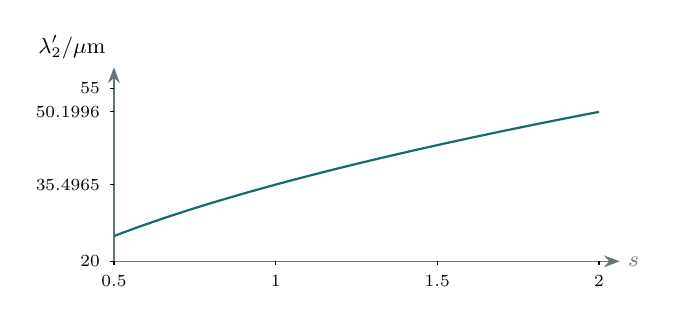
\begin{tikzpicture}[scale=.88,transform shape]
\draw[axis] (0,0)--(7.3,0) node[right] {$s$};
\draw[axis] (0,0)--(0,2.8);
\node[above left] at (0,2.8) {$\lambda_2^\prime/{\rm \mu m}$};
\draw[thin] (0.000000,0)--(0.000000,-0.06);\node[below,font=\scriptsize] at (0.000000,-0.08) {$ 0.5 $};
\draw[thin] (2.333333,0)--(2.333333,-0.06);\node[below,font=\scriptsize] at (2.333333,-0.08) {$ 1 $};
\draw[thin] (4.666667,0)--(4.666667,-0.06);\node[below,font=\scriptsize] at (4.666667,-0.08) {$ 1.5 $};
\draw[thin] (7.000000,0)--(7.000000,-0.06);\node[below,font=\scriptsize] at (7.000000,-0.08) {$ 2 $};
\draw[thin] (0,0.000000)--(-.06,0.000000);\node[left,font=\scriptsize] at (-.08,0.000000) {$ 20 $};
\draw[thin] (0,1.106893)--(-.06,1.106893);\node[left,font=\scriptsize] at (-.08,1.106893) {$ 35.4965 $};
\draw[thin] (0,2.157114)--(-.06,2.157114);\node[left,font=\scriptsize] at (-.08,2.157114) {$ 50.1996 $};
\draw[thin] (0,2.500000)--(-.06,2.500000);\node[left,font=\scriptsize] at (-.08,2.500000) {$ 55 $};
\draw[thick,color=accent] plot coordinates {(0.0000000,0.3642715) (0.0291667,0.3754420) (0.0583333,0.3865437) (0.0875000,0.3975779) (0.1166667,0.4085459) (0.1458333,0.4194487) (0.1750000,0.4302877) (0.2041667,0.4410638) (0.2333333,0.4517781) (0.2625000,0.4624317) (0.2916667,0.4730256) (0.3208333,0.4835609) (0.3500000,0.4940384) (0.3791667,0.5044591) (0.4083333,0.5148240) (0.4375000,0.5251338) (0.4666667,0.5353896) (0.4958333,0.5455920) (0.5250000,0.5557421) (0.5541667,0.5658404) (0.5833333,0.5758879) (0.6125000,0.5858853) (0.6416667,0.5958332) (0.6708333,0.6057326) (0.7000000,0.6155840) (0.7291667,0.6253882) (0.7583333,0.6351457) (0.7875000,0.6448574) (0.8166667,0.6545238) (0.8458333,0.6641455) (0.8750000,0.6737232) (0.9041667,0.6832575) (0.9333333,0.6927489) (0.9625000,0.7021981) (0.9916667,0.7116055) (1.0208333,0.7209717) (1.0500000,0.7302973) (1.0791667,0.7395828) (1.1083333,0.7488287) (1.1375000,0.7580355) (1.1666667,0.7672037) (1.1958333,0.7763338) (1.2250000,0.7854262) (1.2541667,0.7944815) (1.2833333,0.8035000) (1.3125000,0.8124822) (1.3416667,0.8214286) (1.3708333,0.8303395) (1.4000000,0.8392154) (1.4291667,0.8480567) (1.4583333,0.8568638) (1.4875000,0.8656371) (1.5166667,0.8743770) (1.5458333,0.8830838) (1.5750000,0.8917580) (1.6041667,0.9003998) (1.6333333,0.9090097) (1.6625000,0.9175880) (1.6916667,0.9261351) (1.7208333,0.9346513) (1.7500000,0.9431368) (1.7791667,0.9515921) (1.8083333,0.9600175) (1.8375000,0.9684133) (1.8666667,0.9767797) (1.8958333,0.9851172) (1.9250000,0.9934260) (1.9541667,1.0017063) (1.9833333,1.0099586) (2.0125000,1.0181830) (2.0416667,1.0263798) (2.0708333,1.0345494) (2.1000000,1.0426920) (2.1291667,1.0508078) (2.1583333,1.0588972) (2.1875000,1.0669603) (2.2166667,1.0749975) (2.2458333,1.0830089) (2.2750000,1.0909949) (2.3041667,1.0989556) (2.3333333,1.1068913) (2.3625000,1.1148023) (2.3916667,1.1226888) (2.4208333,1.1305509) (2.4500000,1.1383890) (2.4791667,1.1462032) (2.5083333,1.1539937) (2.5375000,1.1617609) (2.5666667,1.1695048) (2.5958333,1.1772257) (2.6250000,1.1849238) (2.6541667,1.1925992) (2.6833333,1.2002523) (2.7125000,1.2078832) (2.7416667,1.2154920) (2.7708333,1.2230790) (2.8000000,1.2306444) (2.8291667,1.2381882) (2.8583333,1.2457109) (2.8875000,1.2532124) (2.9166667,1.2606929) (2.9458333,1.2681528) (2.9750000,1.2755920) (3.0041667,1.2830109) (3.0333333,1.2904095) (3.0625000,1.2977880) (3.0916667,1.3051466) (3.1208333,1.3124855) (3.1500000,1.3198047) (3.1791667,1.3271045) (3.2083333,1.3343851) (3.2375000,1.3416465) (3.2666667,1.3488889) (3.2958333,1.3561124) (3.3250000,1.3633173) (3.3541667,1.3705037) (3.3833333,1.3776716) (3.4125000,1.3848213) (3.4416667,1.3919528) (3.4708333,1.3990664) (3.5000000,1.4061621) (3.5291667,1.4132401) (3.5583333,1.4203005) (3.5875000,1.4273435) (3.6166667,1.4343691) (3.6458333,1.4413776) (3.6750000,1.4483689) (3.7041667,1.4553433) (3.7333333,1.4623009) (3.7625000,1.4692418) (3.7916667,1.4761661) (3.8208333,1.4830739) (3.8500000,1.4899654) (3.8791667,1.4968406) (3.9083333,1.5036998) (3.9375000,1.5105429) (3.9666667,1.5173701) (3.9958333,1.5241815) (4.0250000,1.5309773) (4.0541667,1.5377575) (4.0833333,1.5445222) (4.1125000,1.5512716) (4.1416667,1.5580057) (4.1708333,1.5647247) (4.2000000,1.5714286) (4.2291667,1.5781175) (4.2583333,1.5847917) (4.2875000,1.5914510) (4.3166667,1.5980958) (4.3458333,1.6047259) (4.3750000,1.6113416) (4.4041667,1.6179430) (4.4333333,1.6245300) (4.4625000,1.6311029) (4.4916667,1.6376617) (4.5208333,1.6442065) (4.5500000,1.6507374) (4.5791667,1.6572545) (4.6083333,1.6637578) (4.6375000,1.6702475) (4.6666667,1.6767236) (4.6958333,1.6831862) (4.7250000,1.6896355) (4.7541667,1.6960714) (4.7833333,1.7024941) (4.8125000,1.7089037) (4.8416667,1.7153002) (4.8708333,1.7216837) (4.9000000,1.7280543) (4.9291667,1.7344120) (4.9583333,1.7407570) (4.9875000,1.7470894) (5.0166667,1.7534091) (5.0458333,1.7597163) (5.0750000,1.7660110) (5.1041667,1.7722934) (5.1333333,1.7785635) (5.1625000,1.7848213) (5.1916667,1.7910670) (5.2208333,1.7973005) (5.2500000,1.8035221) (5.2791667,1.8097317) (5.3083333,1.8159294) (5.3375000,1.8221153) (5.3666667,1.8282895) (5.3958333,1.8344519) (5.4250000,1.8406028) (5.4541667,1.8467421) (5.4833333,1.8528699) (5.5125000,1.8589863) (5.5416667,1.8650913) (5.5708333,1.8711851) (5.6000000,1.8772676) (5.6291667,1.8833389) (5.6583333,1.8893991) (5.6875000,1.8954483) (5.7166667,1.9014865) (5.7458333,1.9075137) (5.7750000,1.9135301) (5.8041667,1.9195357) (5.8333333,1.9255305) (5.8625000,1.9315147) (5.8916667,1.9374882) (5.9208333,1.9434511) (5.9500000,1.9494035) (5.9791667,1.9553454) (6.0083333,1.9612769) (6.0375000,1.9671980) (6.0666667,1.9731088) (6.0958333,1.9790094) (6.1250000,1.9848998) (6.1541667,1.9907800) (6.1833333,1.9966501) (6.2125000,2.0025102) (6.2416667,2.0083603) (6.2708333,2.0142005) (6.3000000,2.0200308) (6.3291667,2.0258512) (6.3583333,2.0316618) (6.3875000,2.0374627) (6.4166667,2.0432539) (6.4458333,2.0490355) (6.4750000,2.0548075) (6.5041667,2.0605699) (6.5333333,2.0663228) (6.5625000,2.0720663) (6.5916667,2.0778003) (6.6208333,2.0835250) (6.6500000,2.0892404) (6.6791667,2.0949465) (6.7083333,2.1006434) (6.7375000,2.1063311) (6.7666667,2.1120096) (6.7958333,2.1176791) (6.8250000,2.1233395) (6.8541667,2.1289909) (6.8833333,2.1346334) (6.9125000,2.1402669) (6.9416667,2.1458916) (6.9708333,2.1515074) (7.0000000,2.1571144)};
\end{tikzpicture}
\figcaption{变图光5.3V3\quad 两离子质量同比增加使共振波长按平方根增加}
\end{minipage}\end{center}
\item \textbf{局部双振子式的两端延拓。}求该代数模型在$\lambda_0\to0$和$\lambda_0\to\infty$时的$n^2$，并说明与完整高频介电响应的联系。

使用受迫振子形式$\varepsilon_b+\sum C_j\lambda_0^2\lambda_j^2/(\lambda_0^2-\lambda_j^2)$，短波端两项均按$-C_j\lambda_0^2$趋零，所以$n^2\to\varepsilon_b=1.353192$。长波端每项趋$C_j\lambda_j^2$，故$n^2\to6.09$。变图光5.3V4并列这两个延拓值。完整的高频模型还把构成$\varepsilon_b-1$的远处共振写入；频率高于全部束缚共振时，各项都趋零，剩下真空项1。
\begin{center}\begin{minipage}{.98\linewidth}\centering
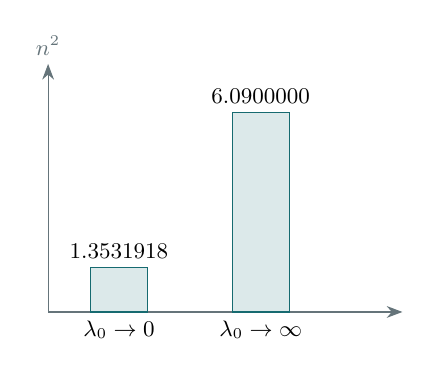
\begin{tikzpicture}[scale=.9,transform shape]
\draw[axis] (0,0)--(5,0);\draw[axis] (0,0)--(0,3.5) node[above] {$n^2$};
\filldraw[fill=accent!15,draw=accent] (0.6,0) rectangle (1.4,0.6245500);\node[above] at (1,0.6245500) {$1.3531918$};\node[below] at (1,0) {$\lambda_0\to0$};
\filldraw[fill=accent!15,draw=accent] (2.6,0) rectangle (3.4,2.8107692);\node[above] at (3,2.8107692) {$6.0900000$};\node[below] at (3,0) {$\lambda_0\to\infty$};
\end{tikzpicture}
\figcaption{变图光5.3V4\quad 局部双振子模型短波与长波两端的代数极限}
\end{minipage}\end{center}
\item \textbf{固定质心后的两离子位移。}取相对位移$\zeta=x_{\rm Ca}-x_{\rm F}$，质心不动。求两个位移，写出动能，并在相反电荷$\pm q$的外电场驱动下给相对坐标方程。

由$40x_{\rm Ca}+19x_{\rm F}=0$和位移差得$x_{\rm Ca}=19\zeta/59$、$x_{\rm F}=-40\zeta/59$，变图光5.3V5的两直线满足这一固定质心关系。动能为
\[
 T=\frac12m_{\rm Ca}\dot x_{\rm Ca}^2+\frac12m_{\rm F}\dot x_{\rm F}^2
 =\frac12\frac{760}{59}m_{\rm H}\dot\zeta^2=\frac12\mu\dot\zeta^2.
\]
回复势为$\kappa\zeta^2/2$，驱动势为$-qE\zeta$，故$\mu\ddot\zeta+\kappa\zeta=qE$。约化质量同时进入本征频率与强度分母。
\begin{center}\begin{minipage}{.98\linewidth}\centering
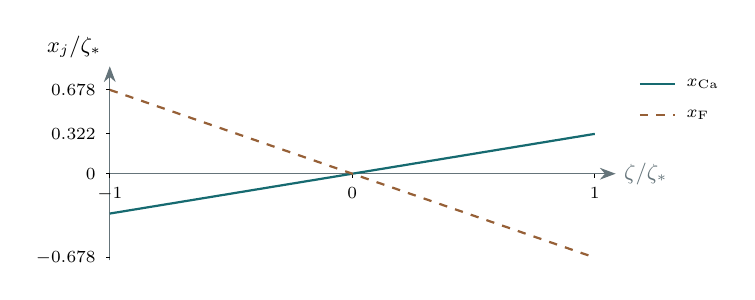
\begin{tikzpicture}[scale=.88,transform shape]
\draw[axis] (0,1.25)--(7.3,1.25) node[right] {$\zeta/\zeta_*$};
\draw[axis] (0,0)--(0,2.8);
\node[above left] at (0,2.8) {$x_j/\zeta_*$};
\draw[thin] (0.000000,1.25)--(0.000000,1.19);\node[below,font=\scriptsize] at (0.000000,1.17) {$ -1 $};
\draw[thin] (3.500000,1.25)--(3.500000,1.19);\node[below,font=\scriptsize] at (3.500000,1.17) {$ 0 $};
\draw[thin] (7.000000,1.25)--(7.000000,1.19);\node[below,font=\scriptsize] at (7.000000,1.17) {$ 1 $};
\draw[thin] (0,0.039286)--(-.06,0.039286);\node[left,font=\scriptsize] at (-.08,0.039286) {$ -0.678 $};
\draw[thin] (0,1.250000)--(-.06,1.250000);\node[left,font=\scriptsize] at (-.08,1.250000) {$ 0 $};
\draw[thin] (0,1.825000)--(-.06,1.825000);\node[left,font=\scriptsize] at (-.08,1.825000) {$ 0.322 $};
\draw[thin] (0,2.460714)--(-.06,2.460714);\node[left,font=\scriptsize] at (-.08,2.460714) {$ 0.678 $};
\draw[thick,color=accent] plot coordinates {(0.0000000,0.6749395) (0.0291667,0.6797316) (0.0583333,0.6845238) (0.0875000,0.6893160) (0.1166667,0.6941082) (0.1458333,0.6989003) (0.1750000,0.7036925) (0.2041667,0.7084847) (0.2333333,0.7132768) (0.2625000,0.7180690) (0.2916667,0.7228612) (0.3208333,0.7276533) (0.3500000,0.7324455) (0.3791667,0.7372377) (0.4083333,0.7420299) (0.4375000,0.7468220) (0.4666667,0.7516142) (0.4958333,0.7564064) (0.5250000,0.7611985) (0.5541667,0.7659907) (0.5833333,0.7707829) (0.6125000,0.7755751) (0.6416667,0.7803672) (0.6708333,0.7851594) (0.7000000,0.7899516) (0.7291667,0.7947437) (0.7583333,0.7995359) (0.7875000,0.8043281) (0.8166667,0.8091203) (0.8458333,0.8139124) (0.8750000,0.8187046) (0.9041667,0.8234968) (0.9333333,0.8282889) (0.9625000,0.8330811) (0.9916667,0.8378733) (1.0208333,0.8426655) (1.0500000,0.8474576) (1.0791667,0.8522498) (1.1083333,0.8570420) (1.1375000,0.8618341) (1.1666667,0.8666263) (1.1958333,0.8714185) (1.2250000,0.8762107) (1.2541667,0.8810028) (1.2833333,0.8857950) (1.3125000,0.8905872) (1.3416667,0.8953793) (1.3708333,0.9001715) (1.4000000,0.9049637) (1.4291667,0.9097559) (1.4583333,0.9145480) (1.4875000,0.9193402) (1.5166667,0.9241324) (1.5458333,0.9289245) (1.5750000,0.9337167) (1.6041667,0.9385089) (1.6333333,0.9433010) (1.6625000,0.9480932) (1.6916667,0.9528854) (1.7208333,0.9576776) (1.7500000,0.9624697) (1.7791667,0.9672619) (1.8083333,0.9720541) (1.8375000,0.9768462) (1.8666667,0.9816384) (1.8958333,0.9864306) (1.9250000,0.9912228) (1.9541667,0.9960149) (1.9833333,1.0008071) (2.0125000,1.0055993) (2.0416667,1.0103914) (2.0708333,1.0151836) (2.1000000,1.0199758) (2.1291667,1.0247680) (2.1583333,1.0295601) (2.1875000,1.0343523) (2.2166667,1.0391445) (2.2458333,1.0439366) (2.2750000,1.0487288) (2.3041667,1.0535210) (2.3333333,1.0583132) (2.3625000,1.0631053) (2.3916667,1.0678975) (2.4208333,1.0726897) (2.4500000,1.0774818) (2.4791667,1.0822740) (2.5083333,1.0870662) (2.5375000,1.0918584) (2.5666667,1.0966505) (2.5958333,1.1014427) (2.6250000,1.1062349) (2.6541667,1.1110270) (2.6833333,1.1158192) (2.7125000,1.1206114) (2.7416667,1.1254036) (2.7708333,1.1301957) (2.8000000,1.1349879) (2.8291667,1.1397801) (2.8583333,1.1445722) (2.8875000,1.1493644) (2.9166667,1.1541566) (2.9458333,1.1589487) (2.9750000,1.1637409) (3.0041667,1.1685331) (3.0333333,1.1733253) (3.0625000,1.1781174) (3.0916667,1.1829096) (3.1208333,1.1877018) (3.1500000,1.1924939) (3.1791667,1.1972861) (3.2083333,1.2020783) (3.2375000,1.2068705) (3.2666667,1.2116626) (3.2958333,1.2164548) (3.3250000,1.2212470) (3.3541667,1.2260391) (3.3833333,1.2308313) (3.4125000,1.2356235) (3.4416667,1.2404157) (3.4708333,1.2452078) (3.5000000,1.2500000) (3.5291667,1.2547922) (3.5583333,1.2595843) (3.5875000,1.2643765) (3.6166667,1.2691687) (3.6458333,1.2739609) (3.6750000,1.2787530) (3.7041667,1.2835452) (3.7333333,1.2883374) (3.7625000,1.2931295) (3.7916667,1.2979217) (3.8208333,1.3027139) (3.8500000,1.3075061) (3.8791667,1.3122982) (3.9083333,1.3170904) (3.9375000,1.3218826) (3.9666667,1.3266747) (3.9958333,1.3314669) (4.0250000,1.3362591) (4.0541667,1.3410513) (4.0833333,1.3458434) (4.1125000,1.3506356) (4.1416667,1.3554278) (4.1708333,1.3602199) (4.2000000,1.3650121) (4.2291667,1.3698043) (4.2583333,1.3745964) (4.2875000,1.3793886) (4.3166667,1.3841808) (4.3458333,1.3889730) (4.3750000,1.3937651) (4.4041667,1.3985573) (4.4333333,1.4033495) (4.4625000,1.4081416) (4.4916667,1.4129338) (4.5208333,1.4177260) (4.5500000,1.4225182) (4.5791667,1.4273103) (4.6083333,1.4321025) (4.6375000,1.4368947) (4.6666667,1.4416868) (4.6958333,1.4464790) (4.7250000,1.4512712) (4.7541667,1.4560634) (4.7833333,1.4608555) (4.8125000,1.4656477) (4.8416667,1.4704399) (4.8708333,1.4752320) (4.9000000,1.4800242) (4.9291667,1.4848164) (4.9583333,1.4896086) (4.9875000,1.4944007) (5.0166667,1.4991929) (5.0458333,1.5039851) (5.0750000,1.5087772) (5.1041667,1.5135694) (5.1333333,1.5183616) (5.1625000,1.5231538) (5.1916667,1.5279459) (5.2208333,1.5327381) (5.2500000,1.5375303) (5.2791667,1.5423224) (5.3083333,1.5471146) (5.3375000,1.5519068) (5.3666667,1.5566990) (5.3958333,1.5614911) (5.4250000,1.5662833) (5.4541667,1.5710755) (5.4833333,1.5758676) (5.5125000,1.5806598) (5.5416667,1.5854520) (5.5708333,1.5902441) (5.6000000,1.5950363) (5.6291667,1.5998285) (5.6583333,1.6046207) (5.6875000,1.6094128) (5.7166667,1.6142050) (5.7458333,1.6189972) (5.7750000,1.6237893) (5.8041667,1.6285815) (5.8333333,1.6333737) (5.8625000,1.6381659) (5.8916667,1.6429580) (5.9208333,1.6477502) (5.9500000,1.6525424) (5.9791667,1.6573345) (6.0083333,1.6621267) (6.0375000,1.6669189) (6.0666667,1.6717111) (6.0958333,1.6765032) (6.1250000,1.6812954) (6.1541667,1.6860876) (6.1833333,1.6908797) (6.2125000,1.6956719) (6.2416667,1.7004641) (6.2708333,1.7052563) (6.3000000,1.7100484) (6.3291667,1.7148406) (6.3583333,1.7196328) (6.3875000,1.7244249) (6.4166667,1.7292171) (6.4458333,1.7340093) (6.4750000,1.7388015) (6.5041667,1.7435936) (6.5333333,1.7483858) (6.5625000,1.7531780) (6.5916667,1.7579701) (6.6208333,1.7627623) (6.6500000,1.7675545) (6.6791667,1.7723467) (6.7083333,1.7771388) (6.7375000,1.7819310) (6.7666667,1.7867232) (6.7958333,1.7915153) (6.8250000,1.7963075) (6.8541667,1.8010997) (6.8833333,1.8058918) (6.9125000,1.8106840) (6.9416667,1.8154762) (6.9708333,1.8202684) (7.0000000,1.8250605)};
\draw[thick,color=accent] (7.65,2.55)--(8.15,2.55);\node[right,font=\scriptsize] at (8.2,2.55) {$x_{\rm Ca}$};
\draw[thick,dashed,color=warm] plot coordinates {(0.0000000,2.4606538) (0.0291667,2.4505650) (0.0583333,2.4404762) (0.0875000,2.4303874) (0.1166667,2.4202986) (0.1458333,2.4102098) (0.1750000,2.4001211) (0.2041667,2.3900323) (0.2333333,2.3799435) (0.2625000,2.3698547) (0.2916667,2.3597659) (0.3208333,2.3496772) (0.3500000,2.3395884) (0.3791667,2.3294996) (0.4083333,2.3194108) (0.4375000,2.3093220) (0.4666667,2.2992333) (0.4958333,2.2891445) (0.5250000,2.2790557) (0.5541667,2.2689669) (0.5833333,2.2588781) (0.6125000,2.2487893) (0.6416667,2.2387006) (0.6708333,2.2286118) (0.7000000,2.2185230) (0.7291667,2.2084342) (0.7583333,2.1983454) (0.7875000,2.1882567) (0.8166667,2.1781679) (0.8458333,2.1680791) (0.8750000,2.1579903) (0.9041667,2.1479015) (0.9333333,2.1378128) (0.9625000,2.1277240) (0.9916667,2.1176352) (1.0208333,2.1075464) (1.0500000,2.0974576) (1.0791667,2.0873688) (1.1083333,2.0772801) (1.1375000,2.0671913) (1.1666667,2.0571025) (1.1958333,2.0470137) (1.2250000,2.0369249) (1.2541667,2.0268362) (1.2833333,2.0167474) (1.3125000,2.0066586) (1.3416667,1.9965698) (1.3708333,1.9864810) (1.4000000,1.9763923) (1.4291667,1.9663035) (1.4583333,1.9562147) (1.4875000,1.9461259) (1.5166667,1.9360371) (1.5458333,1.9259483) (1.5750000,1.9158596) (1.6041667,1.9057708) (1.6333333,1.8956820) (1.6625000,1.8855932) (1.6916667,1.8755044) (1.7208333,1.8654157) (1.7500000,1.8553269) (1.7791667,1.8452381) (1.8083333,1.8351493) (1.8375000,1.8250605) (1.8666667,1.8149718) (1.8958333,1.8048830) (1.9250000,1.7947942) (1.9541667,1.7847054) (1.9833333,1.7746166) (2.0125000,1.7645278) (2.0416667,1.7544391) (2.0708333,1.7443503) (2.1000000,1.7342615) (2.1291667,1.7241727) (2.1583333,1.7140839) (2.1875000,1.7039952) (2.2166667,1.6939064) (2.2458333,1.6838176) (2.2750000,1.6737288) (2.3041667,1.6636400) (2.3333333,1.6535513) (2.3625000,1.6434625) (2.3916667,1.6333737) (2.4208333,1.6232849) (2.4500000,1.6131961) (2.4791667,1.6031073) (2.5083333,1.5930186) (2.5375000,1.5829298) (2.5666667,1.5728410) (2.5958333,1.5627522) (2.6250000,1.5526634) (2.6541667,1.5425747) (2.6833333,1.5324859) (2.7125000,1.5223971) (2.7416667,1.5123083) (2.7708333,1.5022195) (2.8000000,1.4921308) (2.8291667,1.4820420) (2.8583333,1.4719532) (2.8875000,1.4618644) (2.9166667,1.4517756) (2.9458333,1.4416868) (2.9750000,1.4315981) (3.0041667,1.4215093) (3.0333333,1.4114205) (3.0625000,1.4013317) (3.0916667,1.3912429) (3.1208333,1.3811542) (3.1500000,1.3710654) (3.1791667,1.3609766) (3.2083333,1.3508878) (3.2375000,1.3407990) (3.2666667,1.3307103) (3.2958333,1.3206215) (3.3250000,1.3105327) (3.3541667,1.3004439) (3.3833333,1.2903551) (3.4125000,1.2802663) (3.4416667,1.2701776) (3.4708333,1.2600888) (3.5000000,1.2500000) (3.5291667,1.2399112) (3.5583333,1.2298224) (3.5875000,1.2197337) (3.6166667,1.2096449) (3.6458333,1.1995561) (3.6750000,1.1894673) (3.7041667,1.1793785) (3.7333333,1.1692897) (3.7625000,1.1592010) (3.7916667,1.1491122) (3.8208333,1.1390234) (3.8500000,1.1289346) (3.8791667,1.1188458) (3.9083333,1.1087571) (3.9375000,1.0986683) (3.9666667,1.0885795) (3.9958333,1.0784907) (4.0250000,1.0684019) (4.0541667,1.0583132) (4.0833333,1.0482244) (4.1125000,1.0381356) (4.1416667,1.0280468) (4.1708333,1.0179580) (4.2000000,1.0078692) (4.2291667,0.9977805) (4.2583333,0.9876917) (4.2875000,0.9776029) (4.3166667,0.9675141) (4.3458333,0.9574253) (4.3750000,0.9473366) (4.4041667,0.9372478) (4.4333333,0.9271590) (4.4625000,0.9170702) (4.4916667,0.9069814) (4.5208333,0.8968927) (4.5500000,0.8868039) (4.5791667,0.8767151) (4.6083333,0.8666263) (4.6375000,0.8565375) (4.6666667,0.8464487) (4.6958333,0.8363600) (4.7250000,0.8262712) (4.7541667,0.8161824) (4.7833333,0.8060936) (4.8125000,0.7960048) (4.8416667,0.7859161) (4.8708333,0.7758273) (4.9000000,0.7657385) (4.9291667,0.7556497) (4.9583333,0.7455609) (4.9875000,0.7354722) (5.0166667,0.7253834) (5.0458333,0.7152946) (5.0750000,0.7052058) (5.1041667,0.6951170) (5.1333333,0.6850282) (5.1625000,0.6749395) (5.1916667,0.6648507) (5.2208333,0.6547619) (5.2500000,0.6446731) (5.2791667,0.6345843) (5.3083333,0.6244956) (5.3375000,0.6144068) (5.3666667,0.6043180) (5.3958333,0.5942292) (5.4250000,0.5841404) (5.4541667,0.5740517) (5.4833333,0.5639629) (5.5125000,0.5538741) (5.5416667,0.5437853) (5.5708333,0.5336965) (5.6000000,0.5236077) (5.6291667,0.5135190) (5.6583333,0.5034302) (5.6875000,0.4933414) (5.7166667,0.4832526) (5.7458333,0.4731638) (5.7750000,0.4630751) (5.8041667,0.4529863) (5.8333333,0.4428975) (5.8625000,0.4328087) (5.8916667,0.4227199) (5.9208333,0.4126312) (5.9500000,0.4025424) (5.9791667,0.3924536) (6.0083333,0.3823648) (6.0375000,0.3722760) (6.0666667,0.3621872) (6.0958333,0.3520985) (6.1250000,0.3420097) (6.1541667,0.3319209) (6.1833333,0.3218321) (6.2125000,0.3117433) (6.2416667,0.3016546) (6.2708333,0.2915658) (6.3000000,0.2814770) (6.3291667,0.2713882) (6.3583333,0.2612994) (6.3875000,0.2512107) (6.4166667,0.2411219) (6.4458333,0.2310331) (6.4750000,0.2209443) (6.5041667,0.2108555) (6.5333333,0.2007667) (6.5625000,0.1906780) (6.5916667,0.1805892) (6.6208333,0.1705004) (6.6500000,0.1604116) (6.6791667,0.1503228) (6.7083333,0.1402341) (6.7375000,0.1301453) (6.7666667,0.1200565) (6.7958333,0.1099677) (6.8250000,0.0998789) (6.8541667,0.0897902) (6.8833333,0.0797014) (6.9125000,0.0696126) (6.9416667,0.0595238) (6.9708333,0.0494350) (7.0000000,0.0393462)};
\draw[thick,dashed,color=warm] (7.65,2.0999999999999996)--(8.15,2.0999999999999996);\node[right,font=\scriptsize] at (8.2,2.0999999999999996) {$x_{\rm F}$};
\end{tikzpicture}
\figcaption{变图光5.3V5\quad 质心固定时两质量块按相反方向分担相对位移}
\end{minipage}\end{center}
\item \textbf{以给定参照质量比反求有效电荷组合。}若取参照$m_{\rm H}/m_e=1840$，由同一残数求$S=N_2q_2^2/(N_1q_1^2)$；若数密度相同，求电荷比。

由$R=S/[(760/59)M]$，得$S=R(760/59)1840=.9810316$。数密度相同时$|q_2/q_1|=\sqrt S=.9904704$。变图光5.3V6画出一般计数比$\sigma$下$|q_2/q_1|=\sqrt{S/\sigma}$，同一残数允许沿曲线改变两项有效参数。主解等数、等电荷估计与参照之间的差异可由这一小的强度修正表示。
\begin{center}\begin{minipage}{.98\linewidth}\centering
\begin{tikzpicture}[scale=.88,transform shape]
\draw[axis] (0,0)--(7.3,0) node[right] {$\sigma=N_2/N_1$};
\draw[axis] (0,0)--(0,2.8);
\node[above left] at (0,2.8) {$|q_2/q_1|$};
\draw[thin] (0.000000,0)--(0.000000,-0.06);\node[below,font=\scriptsize] at (0.000000,-0.08) {$ 0.5 $};
\draw[thin] (3.500000,0)--(3.500000,-0.06);\node[below,font=\scriptsize] at (3.500000,-0.08) {$ 1 $};
\draw[thin] (7.000000,0)--(7.000000,-0.06);\node[below,font=\scriptsize] at (7.000000,-0.08) {$ 1.5 $};
\draw[thin] (0,0.178571)--(-.06,0.178571);\node[left,font=\scriptsize] at (-.08,0.178571) {$ 0.8 $};
\draw[thin] (0,0.858821)--(-.06,0.858821);\node[left,font=\scriptsize] at (-.08,0.858821) {$ 0.99047 $};
\draw[thin] (0,1.607143)--(-.06,1.607143);\node[left,font=\scriptsize] at (-.08,1.607143) {$ 1.2 $};
\draw[thin] (0,2.321429)--(-.06,2.321429);\node[left,font=\scriptsize] at (-.08,2.321429) {$ 1.4 $};
\draw[thick,color=accent] plot coordinates {(0.0000000,2.3240595) (0.0291667,2.3033446) (0.0583333,2.2828849) (0.0875000,2.2626752) (0.1166667,2.2427105) (0.1458333,2.2229859) (0.1750000,2.2034965) (0.2041667,2.1842378) (0.2333333,2.1652052) (0.2625000,2.1463943) (0.2916667,2.1278009) (0.3208333,2.1094208) (0.3500000,2.0912500) (0.3791667,2.0732845) (0.4083333,2.0555205) (0.4375000,2.0379543) (0.4666667,2.0205821) (0.4958333,2.0034005) (0.5250000,1.9864060) (0.5541667,1.9695952) (0.5833333,1.9529649) (0.6125000,1.9365117) (0.6416667,1.9202327) (0.6708333,1.9041248) (0.7000000,1.8881849) (0.7291667,1.8724103) (0.7583333,1.8567979) (0.7875000,1.8413452) (0.8166667,1.8260493) (0.8458333,1.8109077) (0.8750000,1.7959177) (0.9041667,1.7810769) (0.9333333,1.7663828) (0.9625000,1.7518330) (0.9916667,1.7374252) (1.0208333,1.7231570) (1.0500000,1.7090262) (1.0791667,1.6950306) (1.1083333,1.6811681) (1.1375000,1.6674366) (1.1666667,1.6538341) (1.1958333,1.6403584) (1.2250000,1.6270078) (1.2541667,1.6137801) (1.2833333,1.6006737) (1.3125000,1.5876866) (1.3416667,1.5748170) (1.3708333,1.5620632) (1.4000000,1.5494234) (1.4291667,1.5368960) (1.4583333,1.5244793) (1.4875000,1.5121716) (1.5166667,1.4999715) (1.5458333,1.4878773) (1.5750000,1.4758875) (1.6041667,1.4640006) (1.6333333,1.4522151) (1.6625000,1.4405297) (1.6916667,1.4289429) (1.7208333,1.4174533) (1.7500000,1.4060596) (1.7791667,1.3947605) (1.8083333,1.3835546) (1.8375000,1.3724407) (1.8666667,1.3614175) (1.8958333,1.3504838) (1.9250000,1.3396384) (1.9541667,1.3288802) (1.9833333,1.3182078) (2.0125000,1.3076203) (2.0416667,1.2971165) (2.0708333,1.2866953) (2.1000000,1.2763556) (2.1291667,1.2660964) (2.1583333,1.2559166) (2.1875000,1.2458152) (2.2166667,1.2357912) (2.2458333,1.2258436) (2.2750000,1.2159715) (2.3041667,1.2061739) (2.3333333,1.1964498) (2.3625000,1.1867985) (2.3916667,1.1772189) (2.4208333,1.1677101) (2.4500000,1.1582714) (2.4791667,1.1489018) (2.5083333,1.1396005) (2.5375000,1.1303667) (2.5666667,1.1211996) (2.5958333,1.1120983) (2.6250000,1.1030621) (2.6541667,1.0940903) (2.6833333,1.0851820) (2.7125000,1.0763365) (2.7416667,1.0675530) (2.7708333,1.0588310) (2.8000000,1.0501695) (2.8291667,1.0415680) (2.8583333,1.0330258) (2.8875000,1.0245421) (2.9166667,1.0161164) (2.9458333,1.0077479) (2.9750000,0.9994360) (3.0041667,0.9911801) (3.0333333,0.9829795) (3.0625000,0.9748337) (3.0916667,0.9667419) (3.1208333,0.9587038) (3.1500000,0.9507185) (3.1791667,0.9427856) (3.2083333,0.9349045) (3.2375000,0.9270747) (3.2666667,0.9192955) (3.2958333,0.9115665) (3.3250000,0.9038870) (3.3541667,0.8962566) (3.3833333,0.8886748) (3.4125000,0.8811410) (3.4416667,0.8736547) (3.4708333,0.8662155) (3.5000000,0.8588228) (3.5291667,0.8514762) (3.5583333,0.8441752) (3.5875000,0.8369193) (3.6166667,0.8297080) (3.6458333,0.8225409) (3.6750000,0.8154176) (3.7041667,0.8083376) (3.7333333,0.8013004) (3.7625000,0.7943057) (3.7916667,0.7873530) (3.8208333,0.7804418) (3.8500000,0.7735719) (3.8791667,0.7667427) (3.9083333,0.7599539) (3.9375000,0.7532051) (3.9666667,0.7464958) (3.9958333,0.7398258) (4.0250000,0.7331946) (4.0541667,0.7266018) (4.0833333,0.7200471) (4.1125000,0.7135300) (4.1416667,0.7070504) (4.1708333,0.7006077) (4.2000000,0.6942017) (4.2291667,0.6878319) (4.2583333,0.6814982) (4.2875000,0.6752000) (4.3166667,0.6689371) (4.3458333,0.6627092) (4.3750000,0.6565159) (4.4041667,0.6503569) (4.4333333,0.6442319) (4.4625000,0.6381406) (4.4916667,0.6320827) (4.5208333,0.6260578) (4.5500000,0.6200657) (4.5791667,0.6141061) (4.6083333,0.6081787) (4.6375000,0.6022832) (4.6666667,0.5964193) (4.6958333,0.5905867) (4.7250000,0.5847852) (4.7541667,0.5790144) (4.7833333,0.5732742) (4.8125000,0.5675642) (4.8416667,0.5618842) (4.8708333,0.5562338) (4.9000000,0.5506130) (4.9291667,0.5450213) (4.9583333,0.5394586) (4.9875000,0.5339246) (5.0166667,0.5284190) (5.0458333,0.5229416) (5.0750000,0.5174923) (5.1041667,0.5120706) (5.1333333,0.5066764) (5.1625000,0.5013095) (5.1916667,0.4959697) (5.2208333,0.4906566) (5.2500000,0.4853702) (5.2791667,0.4801101) (5.3083333,0.4748762) (5.3375000,0.4696682) (5.3666667,0.4644859) (5.3958333,0.4593291) (5.4250000,0.4541976) (5.4541667,0.4490912) (5.4833333,0.4440097) (5.5125000,0.4389529) (5.5416667,0.4339206) (5.5708333,0.4289125) (5.6000000,0.4239286) (5.6291667,0.4189685) (5.6583333,0.4140322) (5.6875000,0.4091194) (5.7166667,0.4042300) (5.7458333,0.3993637) (5.7750000,0.3945203) (5.8041667,0.3896998) (5.8333333,0.3849019) (5.8625000,0.3801264) (5.8916667,0.3753732) (5.9208333,0.3706420) (5.9500000,0.3659328) (5.9791667,0.3612454) (6.0083333,0.3565795) (6.0375000,0.3519350) (6.0666667,0.3473118) (6.0958333,0.3427097) (6.1250000,0.3381285) (6.1541667,0.3335681) (6.1833333,0.3290284) (6.2125000,0.3245091) (6.2416667,0.3200101) (6.2708333,0.3155312) (6.3000000,0.3110724) (6.3291667,0.3066334) (6.3583333,0.3022142) (6.3875000,0.2978145) (6.4166667,0.2934342) (6.4458333,0.2890732) (6.4750000,0.2847314) (6.5041667,0.2804086) (6.5333333,0.2761046) (6.5625000,0.2718193) (6.5916667,0.2675527) (6.6208333,0.2633045) (6.6500000,0.2590746) (6.6791667,0.2548629) (6.7083333,0.2506693) (6.7375000,0.2464936) (6.7666667,0.2423358) (6.7958333,0.2381956) (6.8250000,0.2340729) (6.8541667,0.2299677) (6.8833333,0.2258798) (6.9125000,0.2218091) (6.9416667,0.2177555) (6.9708333,0.2137188) (7.0000000,0.2096989)};
\end{tikzpicture}
\figcaption{变图光5.3V6\quad 参照质量比1840给出计数与有效电荷的允许组合}
\end{minipage}\end{center}
\item \textbf{由双共振式求群折射率。}在透明测量窗口求$n_g$，并取真空波长589.3nm给相速、群速所用的两个折射率。

记$F=n^2=6.09+\sum A_j/(\lambda_0^2-a_j)$。求导有$F'=-2\lambda_0\sum A_j/(\lambda_0^2-a_j)^2$，所以
\[
 n'= -\frac{\lambda_0}{n}\sum_j\frac{A_j}{(\lambda_0^2-a_j)^2},\qquad
 n_g=n-\lambda_0n'=n+\frac{\lambda_0^2}{n}\sum_j\frac{A_j}{(\lambda_0^2-a_j)^2}.
\]
变图光5.3V7中$n_g>n$。在589.3nm，$n=1.4350437,n_g=1.4487549$，故$v_p=c/n$、$v_g=c/n_g<v_p$。同一组极点残数的导数决定群延迟，背景进入折射率分母。
\begin{center}\begin{minipage}{.98\linewidth}\centering
\begin{tikzpicture}[scale=.88,transform shape]
\draw[axis] (0,0)--(7.3,0) node[right] {$\lambda_0/{\rm \mu m}$};
\draw[axis] (0,0)--(0,2.8);
\node[above left] at (0,2.8) {$\text{折射率}$};
\draw[thin] (0.000000,0)--(0.000000,-0.06);\node[below,font=\scriptsize] at (0.000000,-0.08) {$ 0.3 $};
\draw[thin] (0.505155,0)--(0.505155,-0.06);\node[below,font=\scriptsize] at (0.505155,-0.08) {$ 1 $};
\draw[thin] (1.948454,0)--(1.948454,-0.06);\node[below,font=\scriptsize] at (1.948454,-0.08) {$ 3 $};
\draw[thin] (3.391753,0)--(3.391753,-0.06);\node[below,font=\scriptsize] at (3.391753,-0.08) {$ 5 $};
\draw[thin] (7.000000,0)--(7.000000,-0.06);\node[below,font=\scriptsize] at (7.000000,-0.08) {$ 10 $};
\draw[thin] (0,0.312500)--(-.06,0.312500);\node[left,font=\scriptsize] at (-.08,0.312500) {$ 1.3 $};
\draw[thin] (0,0.937500)--(-.06,0.937500);\node[left,font=\scriptsize] at (-.08,0.937500) {$ 1.4 $};
\draw[thin] (0,1.562500)--(-.06,1.562500);\node[left,font=\scriptsize] at (-.08,1.562500) {$ 1.5 $};
\draw[thin] (0,2.187500)--(-.06,2.187500);\node[left,font=\scriptsize] at (-.08,2.187500) {$ 1.6 $};
\draw[thick,color=accent] plot coordinates {(0.0000000,1.2823466) (0.0291667,1.2428917) (0.0583333,1.2162390) (0.0875000,1.1972948) (0.1166667,1.1832858) (0.1458333,1.1725889) (0.1750000,1.1641993) (0.2041667,1.1574661) (0.2333333,1.1519522) (0.2625000,1.1473545) (0.2916667,1.1434577) (0.3208333,1.1401047) (0.3500000,1.1371794) (0.3791667,1.1345936) (0.4083333,1.1322802) (0.4375000,1.1301866) (0.4666667,1.1282716) (0.4958333,1.1265024) (0.5250000,1.1248526) (0.5541667,1.1233008) (0.5833333,1.1218293) (0.6125000,1.1204237) (0.6416667,1.1190721) (0.6708333,1.1177642) (0.7000000,1.1164917) (0.7291667,1.1152473) (0.7583333,1.1140250) (0.7875000,1.1128194) (0.8166667,1.1116262) (0.8458333,1.1104413) (0.8750000,1.1092614) (0.9041667,1.1080837) (0.9333333,1.1069054) (0.9625000,1.1057243) (0.9916667,1.1045384) (1.0208333,1.1033461) (1.0500000,1.1021456) (1.0791667,1.1009356) (1.1083333,1.0997149) (1.1375000,1.0984823) (1.1666667,1.0972369) (1.1958333,1.0959777) (1.2250000,1.0947039) (1.2541667,1.0934148) (1.2833333,1.0921098) (1.3125000,1.0907882) (1.3416667,1.0894494) (1.3708333,1.0880929) (1.4000000,1.0867184) (1.4291667,1.0853253) (1.4583333,1.0839133) (1.4875000,1.0824820) (1.5166667,1.0810310) (1.5458333,1.0795601) (1.5750000,1.0780690) (1.6041667,1.0765574) (1.6333333,1.0750250) (1.6625000,1.0734716) (1.6916667,1.0718969) (1.7208333,1.0703009) (1.7500000,1.0686833) (1.7791667,1.0670438) (1.8083333,1.0653824) (1.8375000,1.0636988) (1.8666667,1.0619929) (1.8958333,1.0602645) (1.9250000,1.0585136) (1.9541667,1.0567399) (1.9833333,1.0549434) (2.0125000,1.0531239) (2.0416667,1.0512812) (2.0708333,1.0494154) (2.1000000,1.0475262) (2.1291667,1.0456135) (2.1583333,1.0436773) (2.1875000,1.0417174) (2.2166667,1.0397337) (2.2458333,1.0377262) (2.2750000,1.0356948) (2.3041667,1.0336392) (2.3333333,1.0315596) (2.3625000,1.0294557) (2.3916667,1.0273275) (2.4208333,1.0251749) (2.4500000,1.0229977) (2.4791667,1.0207961) (2.5083333,1.0185697) (2.5375000,1.0163186) (2.5666667,1.0140427) (2.5958333,1.0117418) (2.6250000,1.0094160) (2.6541667,1.0070651) (2.6833333,1.0046890) (2.7125000,1.0022878) (2.7416667,0.9998612) (2.7708333,0.9974092) (2.8000000,0.9949317) (2.8291667,0.9924287) (2.8583333,0.9899001) (2.8875000,0.9873458) (2.9166667,0.9847657) (2.9458333,0.9821597) (2.9750000,0.9795278) (3.0041667,0.9768699) (3.0333333,0.9741859) (3.0625000,0.9714756) (3.0916667,0.9687392) (3.1208333,0.9659764) (3.1500000,0.9631872) (3.1791667,0.9603715) (3.2083333,0.9575292) (3.2375000,0.9546602) (3.2666667,0.9517645) (3.2958333,0.9488420) (3.3250000,0.9458925) (3.3541667,0.9429161) (3.3833333,0.9399126) (3.4125000,0.9368819) (3.4416667,0.9338240) (3.4708333,0.9307388) (3.5000000,0.9276261) (3.5291667,0.9244860) (3.5583333,0.9213182) (3.5875000,0.9181228) (3.6166667,0.9148996) (3.6458333,0.9116485) (3.6750000,0.9083695) (3.7041667,0.9050624) (3.7333333,0.9017272) (3.7625000,0.8983638) (3.7916667,0.8949721) (3.8208333,0.8915520) (3.8500000,0.8881033) (3.8791667,0.8846261) (3.9083333,0.8811201) (3.9375000,0.8775854) (3.9666667,0.8740218) (3.9958333,0.8704291) (4.0250000,0.8668074) (4.0541667,0.8631565) (4.0833333,0.8594763) (4.1125000,0.8557667) (4.1416667,0.8520276) (4.1708333,0.8482589) (4.2000000,0.8444605) (4.2291667,0.8406323) (4.2583333,0.8367741) (4.2875000,0.8328859) (4.3166667,0.8289676) (4.3458333,0.8250190) (4.3750000,0.8210401) (4.4041667,0.8170306) (4.4333333,0.8129906) (4.4625000,0.8089199) (4.4916667,0.8048184) (4.5208333,0.8006859) (4.5500000,0.7965224) (4.5791667,0.7923277) (4.6083333,0.7881018) (4.6375000,0.7838444) (4.6666667,0.7795555) (4.6958333,0.7752349) (4.7250000,0.7708825) (4.7541667,0.7664983) (4.7833333,0.7620820) (4.8125000,0.7576335) (4.8416667,0.7531527) (4.8708333,0.7486396) (4.9000000,0.7440939) (4.9291667,0.7395154) (4.9583333,0.7349042) (4.9875000,0.7302600) (5.0166667,0.7255827) (5.0458333,0.7208722) (5.0750000,0.7161284) (5.1041667,0.7113510) (5.1333333,0.7065399) (5.1625000,0.7016951) (5.1916667,0.6968163) (5.2208333,0.6919035) (5.2500000,0.6869564) (5.2791667,0.6819749) (5.3083333,0.6769589) (5.3375000,0.6719082) (5.3666667,0.6668226) (5.3958333,0.6617021) (5.4250000,0.6565464) (5.4541667,0.6513554) (5.4833333,0.6461290) (5.5125000,0.6408669) (5.5416667,0.6355690) (5.5708333,0.6302352) (5.6000000,0.6248652) (5.6291667,0.6194590) (5.6583333,0.6140163) (5.6875000,0.6085370) (5.7166667,0.6030209) (5.7458333,0.5974678) (5.7750000,0.5918775) (5.8041667,0.5862499) (5.8333333,0.5805849) (5.8625000,0.5748821) (5.8916667,0.5691415) (5.9208333,0.5633628) (5.9500000,0.5575458) (5.9791667,0.5516905) (6.0083333,0.5457965) (6.0375000,0.5398637) (6.0666667,0.5338919) (6.0958333,0.5278809) (6.1250000,0.5218305) (6.1541667,0.5157406) (6.1833333,0.5096108) (6.2125000,0.5034410) (6.2416667,0.4972310) (6.2708333,0.4909806) (6.3000000,0.4846895) (6.3291667,0.4783577) (6.3583333,0.4719847) (6.3875000,0.4655705) (6.4166667,0.4591148) (6.4458333,0.4526175) (6.4750000,0.4460781) (6.5041667,0.4394967) (6.5333333,0.4328728) (6.5625000,0.4262063) (6.5916667,0.4194970) (6.6208333,0.4127446) (6.6500000,0.4059489) (6.6791667,0.3991096) (6.7083333,0.3922265) (6.7375000,0.3852994) (6.7666667,0.3783280) (6.7958333,0.3713121) (6.8250000,0.3642513) (6.8541667,0.3571456) (6.8833333,0.3499945) (6.9125000,0.3427978) (6.9416667,0.3355554) (6.9708333,0.3282668) (7.0000000,0.3209319)};
\draw[thick,color=accent] (7.65,2.55)--(8.15,2.55);\node[right,font=\scriptsize] at (8.2,2.55) {$n$};
\draw[thick,dashed,color=warm] plot coordinates {(0.0000000,1.6430917) (0.0291667,1.5116938) (0.0583333,1.4254092) (0.0875000,1.3654613) (0.1166667,1.3220222) (0.1458333,1.2895039) (0.1750000,1.2645222) (0.2041667,1.2449228) (0.2333333,1.2292777) (0.2625000,1.2166084) (0.2916667,1.2062248) (0.3208333,1.1976286) (0.3500000,1.1904524) (0.3791667,1.1844199) (0.4083333,1.1793206) (0.4375000,1.1749912) (0.4666667,1.1713037) (0.4958333,1.1681567) (0.5250000,1.1654685) (0.5541667,1.1631732) (0.5833333,1.1612170) (0.6125000,1.1595556) (0.6416667,1.1581521) (0.6708333,1.1569758) (0.7000000,1.1560009) (0.7291667,1.1552056) (0.7583333,1.1545713) (0.7875000,1.1540822) (0.8166667,1.1537246) (0.8458333,1.1534869) (0.8750000,1.1533589) (0.9041667,1.1533318) (0.9333333,1.1533978) (0.9625000,1.1535503) (0.9916667,1.1537832) (1.0208333,1.1540915) (1.0500000,1.1544704) (1.0791667,1.1549160) (1.1083333,1.1554246) (1.1375000,1.1559929) (1.1666667,1.1566181) (1.1958333,1.1572977) (1.2250000,1.1580293) (1.2541667,1.1588108) (1.2833333,1.1596405) (1.3125000,1.1605166) (1.3416667,1.1614376) (1.3708333,1.1624022) (1.4000000,1.1634092) (1.4291667,1.1644575) (1.4583333,1.1655460) (1.4875000,1.1666738) (1.5166667,1.1678402) (1.5458333,1.1690444) (1.5750000,1.1702857) (1.6041667,1.1715635) (1.6333333,1.1728773) (1.6625000,1.1742266) (1.6916667,1.1756109) (1.7208333,1.1770298) (1.7500000,1.1784829) (1.7791667,1.1799700) (1.8083333,1.1814907) (1.8375000,1.1830448) (1.8666667,1.1846320) (1.8958333,1.1862521) (1.9250000,1.1879050) (1.9541667,1.1895905) (1.9833333,1.1913084) (2.0125000,1.1930586) (2.0416667,1.1948411) (2.0708333,1.1966557) (2.1000000,1.1985023) (2.1291667,1.2003810) (2.1583333,1.2022917) (2.1875000,1.2042344) (2.2166667,1.2062089) (2.2458333,1.2082155) (2.2750000,1.2102540) (2.3041667,1.2123244) (2.3333333,1.2144269) (2.3625000,1.2165614) (2.3916667,1.2187280) (2.4208333,1.2209267) (2.4500000,1.2231577) (2.4791667,1.2254209) (2.5083333,1.2277165) (2.5375000,1.2300446) (2.5666667,1.2324053) (2.5958333,1.2347986) (2.6250000,1.2372246) (2.6541667,1.2396836) (2.6833333,1.2421755) (2.7125000,1.2447006) (2.7416667,1.2472589) (2.7708333,1.2498506) (2.8000000,1.2524759) (2.8291667,1.2551348) (2.8583333,1.2578276) (2.8875000,1.2605544) (2.9166667,1.2633153) (2.9458333,1.2661106) (2.9750000,1.2689404) (3.0041667,1.2718048) (3.0333333,1.2747042) (3.0625000,1.2776385) (3.0916667,1.2806081) (3.1208333,1.2836132) (3.1500000,1.2866539) (3.1791667,1.2897304) (3.2083333,1.2928430) (3.2375000,1.2959918) (3.2666667,1.2991771) (3.2958333,1.3023991) (3.3250000,1.3056580) (3.3541667,1.3089541) (3.3833333,1.3122876) (3.4125000,1.3156587) (3.4416667,1.3190676) (3.4708333,1.3225147) (3.5000000,1.3260001) (3.5291667,1.3295242) (3.5583333,1.3330871) (3.5875000,1.3366891) (3.6166667,1.3403306) (3.6458333,1.3440117) (3.6750000,1.3477328) (3.7041667,1.3514941) (3.7333333,1.3552959) (3.7625000,1.3591385) (3.7916667,1.3630222) (3.8208333,1.3669473) (3.8500000,1.3709141) (3.8791667,1.3749228) (3.9083333,1.3789738) (3.9375000,1.3830675) (3.9666667,1.3872041) (3.9958333,1.3913839) (4.0250000,1.3956073) (4.0541667,1.3998746) (4.0833333,1.4041862) (4.1125000,1.4085423) (4.1416667,1.4129433) (4.1708333,1.4173896) (4.2000000,1.4218816) (4.2291667,1.4264195) (4.2583333,1.4310038) (4.2875000,1.4356348) (4.3166667,1.4403128) (4.3458333,1.4450383) (4.3750000,1.4498117) (4.4041667,1.4546333) (4.4333333,1.4595035) (4.4625000,1.4644228) (4.4916667,1.4693915) (4.5208333,1.4744100) (4.5500000,1.4794787) (4.5791667,1.4845981) (4.6083333,1.4897686) (4.6375000,1.4949906) (4.6666667,1.5002645) (4.6958333,1.5055908) (4.7250000,1.5109700) (4.7541667,1.5164024) (4.7833333,1.5218886) (4.8125000,1.5274290) (4.8416667,1.5330240) (4.8708333,1.5386742) (4.9000000,1.5443800) (4.9291667,1.5501420) (4.9583333,1.5559605) (4.9875000,1.5618361) (5.0166667,1.5677694) (5.0458333,1.5737607) (5.0750000,1.5798107) (5.1041667,1.5859198) (5.1333333,1.5920887) (5.1625000,1.5983177) (5.1916667,1.6046076) (5.2208333,1.6109587) (5.2500000,1.6173717) (5.2791667,1.6238472) (5.3083333,1.6303857) (5.3375000,1.6369878) (5.3666667,1.6436541) (5.3958333,1.6503852) (5.4250000,1.6571816) (5.4541667,1.6640441) (5.4833333,1.6709731) (5.5125000,1.6779694) (5.5416667,1.6850335) (5.5708333,1.6921662) (5.6000000,1.6993680) (5.6291667,1.7066397) (5.6583333,1.7139818) (5.6875000,1.7213951) (5.7166667,1.7288802) (5.7458333,1.7364379) (5.7750000,1.7440687) (5.8041667,1.7517736) (5.8333333,1.7595531) (5.8625000,1.7674080) (5.8916667,1.7753390) (5.9208333,1.7833469) (5.9500000,1.7914325) (5.9791667,1.7995964) (6.0083333,1.8078396) (6.0375000,1.8161627) (6.0666667,1.8245666) (6.0958333,1.8330520) (6.1250000,1.8416199) (6.1541667,1.8502710) (6.1833333,1.8590061) (6.2125000,1.8678262) (6.2416667,1.8767320) (6.2708333,1.8857245) (6.3000000,1.8948045) (6.3291667,1.9039730) (6.3583333,1.9132309) (6.3875000,1.9225790) (6.4166667,1.9320183) (6.4458333,1.9415497) (6.4750000,1.9511743) (6.5041667,1.9608930) (6.5333333,1.9707067) (6.5625000,1.9806165) (6.5916667,1.9906234) (6.6208333,2.0007284) (6.6500000,2.0109325) (6.6791667,2.0212369) (6.7083333,2.0316425) (6.7375000,2.0421505) (6.7666667,2.0527620) (6.7958333,2.0634780) (6.8250000,2.0742997) (6.8541667,2.0852283) (6.8833333,2.0962649) (6.9125000,2.1074106) (6.9416667,2.1186668) (6.9708333,2.1300345) (7.0000000,2.1415151)};
\draw[thick,dashed,color=warm] (7.65,2.0999999999999996)--(8.15,2.0999999999999996);\node[right,font=\scriptsize] at (8.2,2.0999999999999996) {$n_g$};
\end{tikzpicture}
\figcaption{变图光5.3V7\quad 同一双共振式的相位与群折射率}
\end{minipage}\end{center}
\item \textbf{用远紫外共振表示额外背景。}取第三共振波长20nm，静态响应为$a_3=\varepsilon_b-1=.353191763$。比较它在0.3至10微米内的响应与常数背景。

第三项为$\chi_3=a_3/[1-(20\,\mathrm{nm}/\lambda_0)^2]$。变图光5.3V8显示它在长波窗口内接近$a_3$。最大相对差出现在300nm处，等于$x/(1-x)$，其中$x=(20/300)^2$，所以$\chi_3=.354768512$，比$a_3$增加$.00157675$，相对约$.4464\%$。波长增大使此差按$\lambda_0^{-2}$减小；把该远处共振取长波常数，便得到主解的有限波段背景。
\begin{center}\begin{minipage}{.98\linewidth}\centering
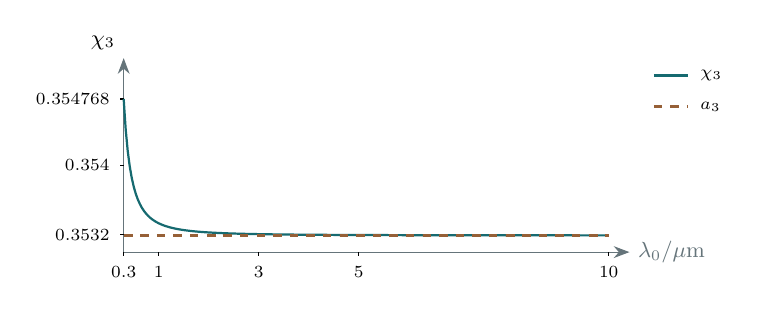
\begin{tikzpicture}[scale=.88,transform shape]
\draw[axis] (0,0)--(7.3,0) node[right] {$\lambda_0/{\rm \mu m}$};
\draw[axis] (0,0)--(0,2.8);
\node[above left] at (0,2.8) {$\chi_3$};
\draw[thin] (0.000000,0)--(0.000000,-0.06);\node[below,font=\scriptsize] at (0.000000,-0.08) {$ 0.3 $};
\draw[thin] (0.505155,0)--(0.505155,-0.06);\node[below,font=\scriptsize] at (0.505155,-0.08) {$ 1 $};
\draw[thin] (1.948454,0)--(1.948454,-0.06);\node[below,font=\scriptsize] at (1.948454,-0.08) {$ 3 $};
\draw[thin] (3.391753,0)--(3.391753,-0.06);\node[below,font=\scriptsize] at (3.391753,-0.08) {$ 5 $};
\draw[thin] (7.000000,0)--(7.000000,-0.06);\node[below,font=\scriptsize] at (7.000000,-0.08) {$ 10 $};
\draw[thin] (0,0.250000)--(-.06,0.250000);\node[left,font=\scriptsize] at (-.08,0.250000) {$ 0.3532 $};
\draw[thin] (0,1.250000)--(-.06,1.250000);\node[left,font=\scriptsize] at (-.08,1.250000) {$ 0.354 $};
\draw[thin] (0,2.210000)--(-.06,2.210000);\node[left,font=\scriptsize] at (-.08,2.210000) {$ 0.354768 $};
\draw[thick,color=accent] plot coordinates {(0.0000000,2.2106402) (0.0291667,1.7688910) (0.0583333,1.4606883) (0.0875000,1.2371303) (0.1166667,1.0698211) (0.1458333,0.9413509) (0.1750000,0.8405619) (0.2041667,0.7600344) (0.2333333,0.6946786) (0.2625000,0.6409087) (0.2916667,0.5961388) (0.3208333,0.5584666) (0.3500000,0.5264671) (0.3791667,0.4990557) (0.4083333,0.4753954) (0.4375000,0.4548316) (0.4666667,0.4368465) (0.4958333,0.4210263) (0.5250000,0.4070369) (0.5541667,0.3946064) (0.5833333,0.3835114) (0.6125000,0.3735672) (0.6416667,0.3646200) (0.6708333,0.3565408) (0.7000000,0.3492208) (0.7291667,0.3425679) (0.7583333,0.3365033) (0.7875000,0.3309597) (0.8166667,0.3258790) (0.8458333,0.3212112) (0.8750000,0.3169126) (0.9041667,0.3129453) (0.9333333,0.3092762) (0.9625000,0.3058760) (0.9916667,0.3027192) (1.0208333,0.2997830) (1.0500000,0.2970473) (1.0791667,0.2944943) (1.1083333,0.2921081) (1.1375000,0.2898745) (1.1666667,0.2877807) (1.1958333,0.2858153) (1.2250000,0.2839680) (1.2541667,0.2822295) (1.2833333,0.2805915) (1.3125000,0.2790463) (1.3416667,0.2775871) (1.3708333,0.2762076) (1.4000000,0.2749021) (1.4291667,0.2736654) (1.4583333,0.2724927) (1.4875000,0.2713798) (1.5166667,0.2703226) (1.5458333,0.2693174) (1.5750000,0.2683610) (1.6041667,0.2674501) (1.6333333,0.2665820) (1.6625000,0.2657540) (1.6916667,0.2649637) (1.7208333,0.2642088) (1.7500000,0.2634872) (1.7791667,0.2627971) (1.8083333,0.2621366) (1.8375000,0.2615040) (1.8666667,0.2608978) (1.8958333,0.2603165) (1.9250000,0.2597588) (1.9541667,0.2592235) (1.9833333,0.2587093) (2.0125000,0.2582151) (2.0416667,0.2577400) (2.0708333,0.2572830) (2.1000000,0.2568431) (2.1291667,0.2564195) (2.1583333,0.2560114) (2.1875000,0.2556181) (2.2166667,0.2552388) (2.2458333,0.2548730) (2.2750000,0.2545199) (2.3041667,0.2541790) (2.3333333,0.2538497) (2.3625000,0.2535316) (2.3916667,0.2532240) (2.4208333,0.2529266) (2.4500000,0.2526389) (2.4791667,0.2523605) (2.5083333,0.2520910) (2.5375000,0.2518300) (2.5666667,0.2515772) (2.5958333,0.2513322) (2.6250000,0.2510947) (2.6541667,0.2508644) (2.6833333,0.2506410) (2.7125000,0.2504243) (2.7416667,0.2502139) (2.7708333,0.2500097) (2.8000000,0.2498114) (2.8291667,0.2496187) (2.8583333,0.2494315) (2.8875000,0.2492495) (2.9166667,0.2490726) (2.9458333,0.2489006) (2.9750000,0.2487333) (3.0041667,0.2485705) (3.0333333,0.2484120) (3.0625000,0.2482578) (3.0916667,0.2481076) (3.1208333,0.2479614) (3.1500000,0.2478189) (3.1791667,0.2476801) (3.2083333,0.2475448) (3.2375000,0.2474130) (3.2666667,0.2472844) (3.2958333,0.2471590) (3.3250000,0.2470367) (3.3541667,0.2469174) (3.3833333,0.2468010) (3.4125000,0.2466874) (3.4416667,0.2465765) (3.4708333,0.2464682) (3.5000000,0.2463624) (3.5291667,0.2462591) (3.5583333,0.2461582) (3.5875000,0.2460596) (3.6166667,0.2459633) (3.6458333,0.2458691) (3.6750000,0.2457770) (3.7041667,0.2456870) (3.7333333,0.2455990) (3.7625000,0.2455129) (3.7916667,0.2454286) (3.8208333,0.2453462) (3.8500000,0.2452656) (3.8791667,0.2451866) (3.9083333,0.2451094) (3.9375000,0.2450337) (3.9666667,0.2449597) (3.9958333,0.2448871) (4.0250000,0.2448161) (4.0541667,0.2447465) (4.0833333,0.2446783) (4.1125000,0.2446115) (4.1416667,0.2445461) (4.1708333,0.2444819) (4.2000000,0.2444190) (4.2291667,0.2443573) (4.2583333,0.2442969) (4.2875000,0.2442376) (4.3166667,0.2441794) (4.3458333,0.2441224) (4.3750000,0.2440664) (4.4041667,0.2440115) (4.4333333,0.2439577) (4.4625000,0.2439048) (4.4916667,0.2438529) (4.5208333,0.2438020) (4.5500000,0.2437520) (4.5791667,0.2437029) (4.6083333,0.2436547) (4.6375000,0.2436073) (4.6666667,0.2435609) (4.6958333,0.2435152) (4.7250000,0.2434703) (4.7541667,0.2434263) (4.7833333,0.2433830) (4.8125000,0.2433404) (4.8416667,0.2432986) (4.8708333,0.2432575) (4.9000000,0.2432171) (4.9291667,0.2431774) (4.9583333,0.2431383) (4.9875000,0.2431000) (5.0166667,0.2430622) (5.0458333,0.2430251) (5.0750000,0.2429886) (5.1041667,0.2429527) (5.1333333,0.2429173) (5.1625000,0.2428826) (5.1916667,0.2428484) (5.2208333,0.2428147) (5.2500000,0.2427816) (5.2791667,0.2427491) (5.3083333,0.2427170) (5.3375000,0.2426854) (5.3666667,0.2426544) (5.3958333,0.2426238) (5.4250000,0.2425937) (5.4541667,0.2425640) (5.4833333,0.2425348) (5.5125000,0.2425061) (5.5416667,0.2424777) (5.5708333,0.2424499) (5.6000000,0.2424224) (5.6291667,0.2423953) (5.6583333,0.2423687) (5.6875000,0.2423424) (5.7166667,0.2423165) (5.7458333,0.2422910) (5.7750000,0.2422659) (5.8041667,0.2422411) (5.8333333,0.2422167) (5.8625000,0.2421927) (5.8916667,0.2421690) (5.9208333,0.2421456) (5.9500000,0.2421226) (5.9791667,0.2420998) (6.0083333,0.2420774) (6.0375000,0.2420554) (6.0666667,0.2420336) (6.0958333,0.2420121) (6.1250000,0.2419909) (6.1541667,0.2419700) (6.1833333,0.2419494) (6.2125000,0.2419291) (6.2416667,0.2419090) (6.2708333,0.2418893) (6.3000000,0.2418697) (6.3291667,0.2418505) (6.3583333,0.2418315) (6.3875000,0.2418127) (6.4166667,0.2417942) (6.4458333,0.2417760) (6.4750000,0.2417579) (6.5041667,0.2417401) (6.5333333,0.2417226) (6.5625000,0.2417053) (6.5916667,0.2416881) (6.6208333,0.2416713) (6.6500000,0.2416546) (6.6791667,0.2416381) (6.7083333,0.2416219) (6.7375000,0.2416058) (6.7666667,0.2415899) (6.7958333,0.2415743) (6.8250000,0.2415588) (6.8541667,0.2415436) (6.8833333,0.2415285) (6.9125000,0.2415136) (6.9416667,0.2414989) (6.9708333,0.2414843) (7.0000000,0.2414700)};
\draw[thick,color=accent] (7.65,2.55)--(8.15,2.55);\node[right,font=\scriptsize] at (8.2,2.55) {$\chi_3$};
\draw[thick,dashed,color=warm] plot coordinates {(0.0000000,0.2397040) (0.0291667,0.2397040) (0.0583333,0.2397040) (0.0875000,0.2397040) (0.1166667,0.2397040) (0.1458333,0.2397040) (0.1750000,0.2397040) (0.2041667,0.2397040) (0.2333333,0.2397040) (0.2625000,0.2397040) (0.2916667,0.2397040) (0.3208333,0.2397040) (0.3500000,0.2397040) (0.3791667,0.2397040) (0.4083333,0.2397040) (0.4375000,0.2397040) (0.4666667,0.2397040) (0.4958333,0.2397040) (0.5250000,0.2397040) (0.5541667,0.2397040) (0.5833333,0.2397040) (0.6125000,0.2397040) (0.6416667,0.2397040) (0.6708333,0.2397040) (0.7000000,0.2397040) (0.7291667,0.2397040) (0.7583333,0.2397040) (0.7875000,0.2397040) (0.8166667,0.2397040) (0.8458333,0.2397040) (0.8750000,0.2397040) (0.9041667,0.2397040) (0.9333333,0.2397040) (0.9625000,0.2397040) (0.9916667,0.2397040) (1.0208333,0.2397040) (1.0500000,0.2397040) (1.0791667,0.2397040) (1.1083333,0.2397040) (1.1375000,0.2397040) (1.1666667,0.2397040) (1.1958333,0.2397040) (1.2250000,0.2397040) (1.2541667,0.2397040) (1.2833333,0.2397040) (1.3125000,0.2397040) (1.3416667,0.2397040) (1.3708333,0.2397040) (1.4000000,0.2397040) (1.4291667,0.2397040) (1.4583333,0.2397040) (1.4875000,0.2397040) (1.5166667,0.2397040) (1.5458333,0.2397040) (1.5750000,0.2397040) (1.6041667,0.2397040) (1.6333333,0.2397040) (1.6625000,0.2397040) (1.6916667,0.2397040) (1.7208333,0.2397040) (1.7500000,0.2397040) (1.7791667,0.2397040) (1.8083333,0.2397040) (1.8375000,0.2397040) (1.8666667,0.2397040) (1.8958333,0.2397040) (1.9250000,0.2397040) (1.9541667,0.2397040) (1.9833333,0.2397040) (2.0125000,0.2397040) (2.0416667,0.2397040) (2.0708333,0.2397040) (2.1000000,0.2397040) (2.1291667,0.2397040) (2.1583333,0.2397040) (2.1875000,0.2397040) (2.2166667,0.2397040) (2.2458333,0.2397040) (2.2750000,0.2397040) (2.3041667,0.2397040) (2.3333333,0.2397040) (2.3625000,0.2397040) (2.3916667,0.2397040) (2.4208333,0.2397040) (2.4500000,0.2397040) (2.4791667,0.2397040) (2.5083333,0.2397040) (2.5375000,0.2397040) (2.5666667,0.2397040) (2.5958333,0.2397040) (2.6250000,0.2397040) (2.6541667,0.2397040) (2.6833333,0.2397040) (2.7125000,0.2397040) (2.7416667,0.2397040) (2.7708333,0.2397040) (2.8000000,0.2397040) (2.8291667,0.2397040) (2.8583333,0.2397040) (2.8875000,0.2397040) (2.9166667,0.2397040) (2.9458333,0.2397040) (2.9750000,0.2397040) (3.0041667,0.2397040) (3.0333333,0.2397040) (3.0625000,0.2397040) (3.0916667,0.2397040) (3.1208333,0.2397040) (3.1500000,0.2397040) (3.1791667,0.2397040) (3.2083333,0.2397040) (3.2375000,0.2397040) (3.2666667,0.2397040) (3.2958333,0.2397040) (3.3250000,0.2397040) (3.3541667,0.2397040) (3.3833333,0.2397040) (3.4125000,0.2397040) (3.4416667,0.2397040) (3.4708333,0.2397040) (3.5000000,0.2397040) (3.5291667,0.2397040) (3.5583333,0.2397040) (3.5875000,0.2397040) (3.6166667,0.2397040) (3.6458333,0.2397040) (3.6750000,0.2397040) (3.7041667,0.2397040) (3.7333333,0.2397040) (3.7625000,0.2397040) (3.7916667,0.2397040) (3.8208333,0.2397040) (3.8500000,0.2397040) (3.8791667,0.2397040) (3.9083333,0.2397040) (3.9375000,0.2397040) (3.9666667,0.2397040) (3.9958333,0.2397040) (4.0250000,0.2397040) (4.0541667,0.2397040) (4.0833333,0.2397040) (4.1125000,0.2397040) (4.1416667,0.2397040) (4.1708333,0.2397040) (4.2000000,0.2397040) (4.2291667,0.2397040) (4.2583333,0.2397040) (4.2875000,0.2397040) (4.3166667,0.2397040) (4.3458333,0.2397040) (4.3750000,0.2397040) (4.4041667,0.2397040) (4.4333333,0.2397040) (4.4625000,0.2397040) (4.4916667,0.2397040) (4.5208333,0.2397040) (4.5500000,0.2397040) (4.5791667,0.2397040) (4.6083333,0.2397040) (4.6375000,0.2397040) (4.6666667,0.2397040) (4.6958333,0.2397040) (4.7250000,0.2397040) (4.7541667,0.2397040) (4.7833333,0.2397040) (4.8125000,0.2397040) (4.8416667,0.2397040) (4.8708333,0.2397040) (4.9000000,0.2397040) (4.9291667,0.2397040) (4.9583333,0.2397040) (4.9875000,0.2397040) (5.0166667,0.2397040) (5.0458333,0.2397040) (5.0750000,0.2397040) (5.1041667,0.2397040) (5.1333333,0.2397040) (5.1625000,0.2397040) (5.1916667,0.2397040) (5.2208333,0.2397040) (5.2500000,0.2397040) (5.2791667,0.2397040) (5.3083333,0.2397040) (5.3375000,0.2397040) (5.3666667,0.2397040) (5.3958333,0.2397040) (5.4250000,0.2397040) (5.4541667,0.2397040) (5.4833333,0.2397040) (5.5125000,0.2397040) (5.5416667,0.2397040) (5.5708333,0.2397040) (5.6000000,0.2397040) (5.6291667,0.2397040) (5.6583333,0.2397040) (5.6875000,0.2397040) (5.7166667,0.2397040) (5.7458333,0.2397040) (5.7750000,0.2397040) (5.8041667,0.2397040) (5.8333333,0.2397040) (5.8625000,0.2397040) (5.8916667,0.2397040) (5.9208333,0.2397040) (5.9500000,0.2397040) (5.9791667,0.2397040) (6.0083333,0.2397040) (6.0375000,0.2397040) (6.0666667,0.2397040) (6.0958333,0.2397040) (6.1250000,0.2397040) (6.1541667,0.2397040) (6.1833333,0.2397040) (6.2125000,0.2397040) (6.2416667,0.2397040) (6.2708333,0.2397040) (6.3000000,0.2397040) (6.3291667,0.2397040) (6.3583333,0.2397040) (6.3875000,0.2397040) (6.4166667,0.2397040) (6.4458333,0.2397040) (6.4750000,0.2397040) (6.5041667,0.2397040) (6.5333333,0.2397040) (6.5625000,0.2397040) (6.5916667,0.2397040) (6.6208333,0.2397040) (6.6500000,0.2397040) (6.6791667,0.2397040) (6.7083333,0.2397040) (6.7375000,0.2397040) (6.7666667,0.2397040) (6.7958333,0.2397040) (6.8250000,0.2397040) (6.8541667,0.2397040) (6.8833333,0.2397040) (6.9125000,0.2397040) (6.9416667,0.2397040) (6.9708333,0.2397040) (7.0000000,0.2397040)};
\draw[thick,dashed,color=warm] (7.65,2.0999999999999996)--(8.15,2.0999999999999996);\node[right,font=\scriptsize] at (8.2,2.0999999999999996) {$a_3$};
\end{tikzpicture}
\figcaption{变图光5.3V8\quad 20nm远共振在透明窗口内表现为接近常数的背景}
\end{minipage}\end{center}
\end{enumerate}

\Needspace{13\baselineskip}

\pdfbookmark[2]{第 4 题 X射线色散及速度乘积}{q4}

\section*{第 4 题\quad X射线色散及速度乘积}\label{q:4}

在X射线频率远高于电子束缚共振频率、损耗可忽略的范围内，证明金属折射率满足$n^2=1-K\lambda_0^2$。对铜取原子序数29、相对原子质量63、密度$8.0\times10^3\,\mathrm{kg/m^3}$，估算$K$；再证明该模型内相速与群速的乘积为$c^2$。

\begin{center}\begin{minipage}{.98\linewidth}\centering
\begin{tikzpicture}[scale=.9,transform shape]
\draw[axis] (0.00000,0.00000)--(6.80000,0.00000);\draw[axis] (0.00000,-0.15000)--(0.00000,2.30000);\node[below right] at (6.80000,0.00000) {$\omega/\omega_p$};\node[above right] at (0.00000,2.30000) {$n^2$};\draw[traj] plot coordinates {(1.00000,0.00000) (1.03741,0.14164) (1.07482,0.26876) (1.11223,0.38326) (1.14964,0.48677) (1.18705,0.58064) (1.22446,0.66605) (1.26187,0.74397) (1.29928,0.81526) (1.33669,0.88064) (1.37410,0.94076) (1.41151,0.99617) (1.44892,1.04733) (1.48633,1.09469) (1.52374,1.13859) (1.56115,1.17938) (1.59856,1.21734) (1.63597,1.25273) (1.67338,1.28577) (1.71079,1.31666) (1.74820,1.34559) (1.78561,1.37273) (1.82302,1.39821) (1.86043,1.42217) (1.89784,1.44472) (1.93525,1.46598) (1.97266,1.48605) (2.01007,1.50500) (2.04748,1.52292) (2.08489,1.53989) (2.12230,1.55597) (2.15971,1.57122) (2.19712,1.58569) (2.23453,1.59945) (2.27194,1.61253) (2.30935,1.62498) (2.34676,1.63685) (2.38417,1.64815) (2.42158,1.65894) (2.45899,1.66924) (2.49640,1.67908) (2.53381,1.68848) (2.57122,1.69748) (2.60863,1.70610) (2.64604,1.71435) (2.68345,1.72226) (2.72086,1.72984) (2.75827,1.73712) (2.79568,1.74411) (2.83309,1.75082) (2.87050,1.75728) (2.90791,1.76348) (2.94532,1.76945) (2.98273,1.77520) (3.02014,1.78073) (3.05755,1.78607) (3.09496,1.79121) (3.13237,1.79616) (3.16978,1.80095) (3.20719,1.80556) (3.24460,1.81002) (3.28201,1.81433) (3.31942,1.81849) (3.35683,1.82251) (3.39424,1.82640) (3.43165,1.83017) (3.46906,1.83381) (3.50647,1.83734) (3.54388,1.84075) (3.58129,1.84406) (3.61871,1.84727) (3.65612,1.85038) (3.69353,1.85340) (3.73094,1.85632) (3.76835,1.85916) (3.80576,1.86191) (3.84317,1.86459) (3.88058,1.86719) (3.91799,1.86971) (3.95540,1.87216) (3.99281,1.87455) (4.03022,1.87687) (4.06763,1.87912) (4.10504,1.88131) (4.14245,1.88345) (4.17986,1.88553) (4.21727,1.88755) (4.25468,1.88952) (4.29209,1.89143) (4.32950,1.89330) (4.36691,1.89512) (4.40432,1.89690) (4.44173,1.89863) (4.47914,1.90031) (4.51655,1.90196) (4.55396,1.90356) (4.59137,1.90513) (4.62878,1.90665) (4.66619,1.90814) (4.70360,1.90960) (4.74101,1.91102) (4.77842,1.91241) (4.81583,1.91376) (4.85324,1.91509) (4.89065,1.91638) (4.92806,1.91765) (4.96547,1.91888) (5.00288,1.92009) (5.04029,1.92127) (5.07770,1.92243) (5.11511,1.92356) (5.15252,1.92467) (5.18993,1.92575) (5.22734,1.92681) (5.26475,1.92784) (5.30216,1.92886) (5.33957,1.92985) (5.37698,1.93082) (5.41439,1.93178) (5.45180,1.93271) (5.48921,1.93362) (5.52662,1.93452) (5.56403,1.93540) (5.60144,1.93626) (5.63885,1.93710) (5.67626,1.93793) (5.71367,1.93874) (5.75108,1.93953) (5.78849,1.94031) (5.82590,1.94107) (5.86331,1.94182) (5.90072,1.94256) (5.93813,1.94328) (5.97554,1.94399) (6.01295,1.94468) (6.05036,1.94537) (6.08777,1.94603) (6.12518,1.94669) (6.16259,1.94734) (6.20000,1.94797)};\draw[guide] (0.00000,2.00000)--(6.20000,2.00000);\node[left] at (0.00000,2.00000) {1};\node[below] at (1.00000,0.00000) {1};
\end{tikzpicture}
\figcaption{图光5.4\quad 高频传播区的折射率平方从零趋近1。}
\end{minipage}\end{center}

\Needspace{8\baselineskip}

\pdfbookmark[3]{题型定位}{q4-h0}

\subsection*{题型定位}

由束缚电子的高频惯性项求负极化，再把同一折射率关系改写成平方型色散，沿一条曲线求两速度。全电子计数、远离吸收边和传播分支在各自步骤中说明。

\Needspace{8\baselineskip}

\pdfbookmark[3]{知识点}{q4-h1}

\subsection*{知识点}

\begin{itemize}
\item 高频受迫响应与电场反相，给$n^2-1<0$；传播区仍满足$n^2>0$。
\item 此处总电子数密度是原子数密度乘29，全电子高频响应与只计价电子的低频模型使用不同计数。
\item $\omega^2=c^2k^2+\omega_p^2$的原点割线和切线属于同一工作点，分别给相速和群速。
\item 真空波长确定材料色散，介质内波数用于群速度导数，两者由$k=n\omega/c$连接。
\end{itemize}

\Needspace{8\baselineskip}

\pdfbookmark[3]{物理图像}{q4-h2}

\subsection*{物理图像}

解图A的色散线从$\omega_p$起步，工作点的割线较陡、切线较缓；B把两速度随频率并列，C放大X射线折射率的小偏离，D显示电子计数对$K$和频率尺度的不同幂次作用。电子位移与负电荷偶极矩共同解释极化符号。

\Needspace{8\baselineskip}

\pdfbookmark[3]{解题入口}{q4-h3}

\subsection*{解题入口}

先把各束缚分母按$\omega_j^2/\omega^2$展开，求出负的主导项，再算全电子密度。第二问把$n^2$乘$\omega^2$，得到以$k$为自变量的平方型关系，在实传播分支直接求导。

\Needspace{8\baselineskip}

\pdfbookmark[3]{标准解法}{q4-h4}

\subsection*{标准解法}


图光5.4的高频折射率由电子在电场中的惯性响应决定。对第$j$类束缚电子，$m_e(\omega_j^2-\omega^2)x_j=-eE$，偶极矩为$-ex_j$，所以各类电子对色散的贡献为
\[
n^2-1=\sum_j\frac{N_je^2}{\varepsilon_0m_e(\omega_j^2-\omega^2)}.
\]
在$\omega\gg\omega_j$并远离吸收边、损耗很小的范围，$1/(\omega_j^2-\omega^2)=-\omega^{-2}[1+O(\omega_j^2/\omega^2)]$。总电子数密度$N=\sum_jN_j$，把主导项相加有
\[
n^2=1-\frac{Ne^2}{\varepsilon_0m_e\omega^2}
=1-\frac{Ne^2}{4\pi^2\varepsilon_0m_ec^2}\lambda_0^2.
\]
因此$K=Ne^2/(4\pi^2\varepsilon_0m_ec^2)$，单位为$\mathrm{m^{-2}}$。电子的负电荷在位移与偶极矩中各出现一次，留下正的$e^2$；极化的负号由高频惯性分母给出。正离子响应也按电荷平方除以质量加权，其质量大，在该近似中贡献较小。

铜的原子数密度为$\rho N_A/(63\times10^{-3})$，高于全部束缚共振的模型每原子计29个电子，故
\[
N=\frac{29\rho N_A}{63\times10^{-3}}
\simeq2.22\times10^{30}\,\mathrm{m^{-3}},
\qquad
\boxed{K\simeq1.99\times10^{15}\,\mathrm{m^{-2}}}.
\]
用$N_A=6.02214\times10^{23}\,\mathrm{mol^{-1}}$、$e=1.60218\times10^{-19}\,\mathrm C$、$m_e=9.10938\times10^{-31}\,\mathrm{kg}$及$\varepsilon_0=8.85419\times10^{-12}\,\mathrm{F/m}$，得到$N=2.217677\times10^{30}\,\mathrm{m^{-3}}$、$K=1.986465\times10^{15}\,\mathrm{m^{-2}}$。在$.10\,\mathrm{nm}$处，$K\lambda_0^2=1.986465\times10^{-5}$，所以$n=.999990068$。解图光5.4C用$10^6(1-n)$显示这一小偏离；一阶式$1-n\simeq K\lambda_0^2/2$来自平方根展开。
\begin{center}\begin{minipage}{.98\linewidth}\centering
\begin{tikzpicture}[scale=.88,transform shape]
\draw[axis] (0,0.0)--(7.3,0.0) node[right] {$\lambda_0/{\rm nm}$};
\draw[axis] (0,0)--(0,2.8);
\node[above left] at (0,2.8) {$10^6(1-n)$};
\draw[thin] (0.000000,0.0)--(0.000000,-0.06);\node[below,font=\scriptsize] at (0.000000,-0.08) {$ 0.05 $};
\draw[thin] (2.333333,0.0)--(2.333333,-0.06);\node[below,font=\scriptsize] at (2.333333,-0.08) {$ 0.1 $};
\draw[thin] (4.666667,0.0)--(4.666667,-0.06);\node[below,font=\scriptsize] at (4.666667,-0.08) {$ 0.15 $};
\draw[thin] (7.000000,0.0)--(7.000000,-0.06);\node[below,font=\scriptsize] at (7.000000,-0.08) {$ 0.2 $};
\draw[thin] (0,0.000000)--(-.06,0.000000);\node[left,font=\scriptsize] at (-.08,0.000000) {$ 0 $};
\draw[thin] (0,0.595238)--(-.06,0.595238);\node[left,font=\scriptsize] at (-.08,0.595238) {$ 10 $};
\draw[thin] (0,1.190476)--(-.06,1.190476);\node[left,font=\scriptsize] at (-.08,1.190476) {$ 20 $};
\draw[thin] (0,1.785714)--(-.06,1.785714);\node[left,font=\scriptsize] at (-.08,1.785714) {$ 30 $};
\draw[thin] (0,2.380952)--(-.06,2.380952);\node[left,font=\scriptsize] at (-.08,2.380952) {$ 40 $};
\draw[thick,color=accent] plot coordinates {(0.0000000,0.1478027) (0.0291667,0.1515208) (0.0583333,0.1552852) (0.0875000,0.1590957) (0.1166667,0.1629525) (0.1458333,0.1668554) (0.1750000,0.1708045) (0.2041667,0.1747998) (0.2333333,0.1788413) (0.2625000,0.1829289) (0.2916667,0.1870628) (0.3208333,0.1912429) (0.3500000,0.1954691) (0.3791667,0.1997415) (0.4083333,0.2040602) (0.4375000,0.2084250) (0.4666667,0.2128360) (0.4958333,0.2172931) (0.5250000,0.2217965) (0.5541667,0.2263461) (0.5833333,0.2309418) (0.6125000,0.2355838) (0.6416667,0.2402719) (0.6708333,0.2450062) (0.7000000,0.2497867) (0.7291667,0.2546134) (0.7583333,0.2594863) (0.7875000,0.2644054) (0.8166667,0.2693706) (0.8458333,0.2743821) (0.8750000,0.2794397) (0.9041667,0.2845436) (0.9333333,0.2896936) (0.9625000,0.2948898) (0.9916667,0.3001322) (1.0208333,0.3054208) (1.0500000,0.3107555) (1.0791667,0.3161365) (1.1083333,0.3215636) (1.1375000,0.3270370) (1.1666667,0.3325565) (1.1958333,0.3381222) (1.2250000,0.3437341) (1.2541667,0.3493922) (1.2833333,0.3550965) (1.3125000,0.3608470) (1.3416667,0.3666437) (1.3708333,0.3724865) (1.4000000,0.3783756) (1.4291667,0.3843108) (1.4583333,0.3902922) (1.4875000,0.3963198) (1.5166667,0.4023936) (1.5458333,0.4085136) (1.5750000,0.4146798) (1.6041667,0.4208921) (1.6333333,0.4271507) (1.6625000,0.4334554) (1.6916667,0.4398064) (1.7208333,0.4462035) (1.7500000,0.4526468) (1.7791667,0.4591363) (1.8083333,0.4656720) (1.8375000,0.4722539) (1.8666667,0.4788820) (1.8958333,0.4855562) (1.9250000,0.4922767) (1.9541667,0.4990433) (1.9833333,0.5058561) (2.0125000,0.5127152) (2.0416667,0.5196204) (2.0708333,0.5265718) (2.1000000,0.5335693) (2.1291667,0.5406131) (2.1583333,0.5477031) (2.1875000,0.5548392) (2.2166667,0.5620216) (2.2458333,0.5692501) (2.2750000,0.5765248) (2.3041667,0.5838458) (2.3333333,0.5912129) (2.3625000,0.5986262) (2.3916667,0.6060856) (2.4208333,0.6135913) (2.4500000,0.6211432) (2.4791667,0.6287412) (2.5083333,0.6363855) (2.5375000,0.6440759) (2.5666667,0.6518125) (2.5958333,0.6595953) (2.6250000,0.6674243) (2.6541667,0.6752995) (2.6833333,0.6832209) (2.7125000,0.6911885) (2.7416667,0.6992022) (2.7708333,0.7072622) (2.8000000,0.7153683) (2.8291667,0.7235206) (2.8583333,0.7317192) (2.8875000,0.7399639) (2.9166667,0.7482548) (2.9458333,0.7565919) (2.9750000,0.7649751) (3.0041667,0.7734046) (3.0333333,0.7818803) (3.0625000,0.7904021) (3.0916667,0.7989701) (3.1208333,0.8075844) (3.1500000,0.8162448) (3.1791667,0.8249514) (3.2083333,0.8337042) (3.2375000,0.8425032) (3.2666667,0.8513484) (3.2958333,0.8602397) (3.3250000,0.8691773) (3.3541667,0.8781611) (3.3833333,0.8871910) (3.4125000,0.8962671) (3.4416667,0.9053895) (3.4708333,0.9145580) (3.5000000,0.9237727) (3.5291667,0.9330336) (3.5583333,0.9423407) (3.5875000,0.9516939) (3.6166667,0.9610934) (3.6458333,0.9705390) (3.6750000,0.9800309) (3.7041667,0.9895689) (3.7333333,0.9991532) (3.7625000,1.0087836) (3.7916667,1.0184602) (3.8208333,1.0281830) (3.8500000,1.0379520) (3.8791667,1.0477672) (3.9083333,1.0576285) (3.9375000,1.0675361) (3.9666667,1.0774898) (3.9958333,1.0874898) (4.0250000,1.0975359) (4.0541667,1.1076282) (4.0833333,1.1177668) (4.1125000,1.1279515) (4.1416667,1.1381824) (4.1708333,1.1484595) (4.2000000,1.1587827) (4.2291667,1.1691522) (4.2583333,1.1795679) (4.2875000,1.1900297) (4.3166667,1.2005378) (4.3458333,1.2110920) (4.3750000,1.2216924) (4.4041667,1.2323390) (4.4333333,1.2430318) (4.4625000,1.2537708) (4.4916667,1.2645560) (4.5208333,1.2753874) (4.5500000,1.2862650) (4.5791667,1.2971888) (4.6083333,1.3081587) (4.6375000,1.3191749) (4.6666667,1.3302372) (4.6958333,1.3413457) (4.7250000,1.3525004) (4.7541667,1.3637014) (4.7833333,1.3749485) (4.8125000,1.3862418) (4.8416667,1.3975812) (4.8708333,1.4089669) (4.9000000,1.4203988) (4.9291667,1.4318769) (4.9583333,1.4434011) (4.9875000,1.4549715) (5.0166667,1.4665882) (5.0458333,1.4782510) (5.0750000,1.4899600) (5.1041667,1.5017152) (5.1333333,1.5135166) (5.1625000,1.5253642) (5.1916667,1.5372580) (5.2208333,1.5491980) (5.2500000,1.5611842) (5.2791667,1.5732165) (5.3083333,1.5852951) (5.3375000,1.5974198) (5.3666667,1.6095908) (5.3958333,1.6218079) (5.4250000,1.6340712) (5.4541667,1.6463807) (5.4833333,1.6587365) (5.5125000,1.6711384) (5.5416667,1.6835864) (5.5708333,1.6960807) (5.6000000,1.7086212) (5.6291667,1.7212079) (5.6583333,1.7338407) (5.6875000,1.7465198) (5.7166667,1.7592450) (5.7458333,1.7720165) (5.7750000,1.7848341) (5.8041667,1.7976979) (5.8333333,1.8106079) (5.8625000,1.8235641) (5.8916667,1.8365665) (5.9208333,1.8496151) (5.9500000,1.8627099) (5.9791667,1.8758509) (6.0083333,1.8890381) (6.0375000,1.9022714) (6.0666667,1.9155510) (6.0958333,1.9288767) (6.1250000,1.9422487) (6.1541667,1.9556668) (6.1833333,1.9691311) (6.2125000,1.9826416) (6.2416667,1.9961984) (6.2708333,2.0098013) (6.3000000,2.0234504) (6.3291667,2.0371456) (6.3583333,2.0508871) (6.3875000,2.0646748) (6.4166667,2.0785087) (6.4458333,2.0923887) (6.4750000,2.1063150) (6.5041667,2.1202874) (6.5333333,2.1343061) (6.5625000,2.1483709) (6.5916667,2.1624820) (6.6208333,2.1766392) (6.6500000,2.1908426) (6.6791667,2.2050922) (6.7083333,2.2193880) (6.7375000,2.2337300) (6.7666667,2.2481182) (6.7958333,2.2625526) (6.8250000,2.2770331) (6.8541667,2.2915599) (6.8833333,2.3061329) (6.9125000,2.3207520) (6.9416667,2.3354174) (6.9708333,2.3501289) (7.0000000,2.3648867)};
\end{tikzpicture}
\figcaption{解图光5.4C\quad 硬X射线高频模型的折射率小偏离}
\end{minipage}\end{center}
令$\omega_p^2=Ne^2/(\varepsilon_0m_e)=4\pi^2c^2K$，结合$k=n\omega/c$把波长色散写成
\[
c^2k^2=\omega^2-\omega_p^2,\quad
\omega=\sqrt{c^2k^2+\omega_p^2}.
\]
在传播分支$\omega>\omega_p$上取$k>0$，解图光5.4A给出这条有纵轴截距的色散线。通过同一点$P$的原点割线与局部切线分别给相速和群速：
\[
v_p=\frac{\omega}{k}=\frac cn,\qquad
v_g=\frac{\dd\omega}{\dd k}=\frac{c^2k}{\omega}=cn,
\]
\[
\boxed{v_pv_g=c^2}.
\]
用介质内波长还可直接求群速：$\lambda_m=\lambda_0/n$、$1/\lambda_0=\sqrt{(1/\lambda_m)^2+K}$，沿$1/\lambda_m$求导，得到
\[
v_g=\frac{\dd(c/\lambda_0)}{\dd(1/\lambda_m)}
=\frac{c/\lambda_m}{\sqrt{\lambda_m^{-2}+K}}
=\frac{cn}{\sqrt{n^2+K\lambda_0^2}}=cn.
\]这里用真空波长写介质参数，再沿内部波数求导，转换由$\lambda_m=\lambda_0/n$给出。
\begin{center}\begin{minipage}{.98\linewidth}\centering
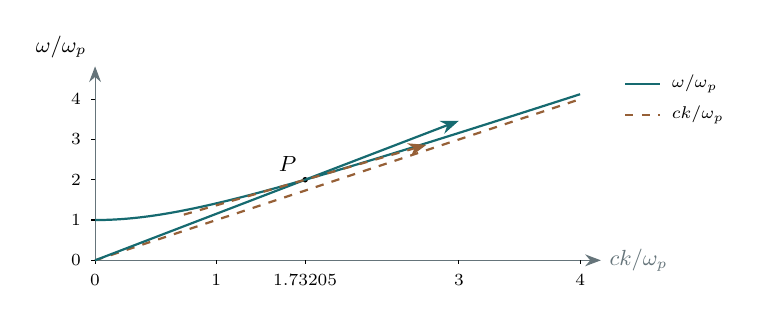
\begin{tikzpicture}[scale=.88,transform shape]
\draw[axis] (0,0.0)--(7.3,0.0) node[right] {$ck/\omega_p$};
\draw[axis] (0,0)--(0,2.8);
\node[above left] at (0,2.8) {$\omega/\omega_p$};
\draw[thin] (0.000000,0.0)--(0.000000,-0.06);\node[below,font=\scriptsize] at (0.000000,-0.08) {$ 0 $};
\draw[thin] (1.750000,0.0)--(1.750000,-0.06);\node[below,font=\scriptsize] at (1.750000,-0.08) {$ 1 $};
\draw[thin] (3.031089,0.0)--(3.031089,-0.06);\node[below,font=\scriptsize] at (3.031089,-0.08) {$ 1.73205 $};
\draw[thin] (5.250000,0.0)--(5.250000,-0.06);\node[below,font=\scriptsize] at (5.250000,-0.08) {$ 3 $};
\draw[thin] (7.000000,0.0)--(7.000000,-0.06);\node[below,font=\scriptsize] at (7.000000,-0.08) {$ 4 $};
\draw[thin] (0,0.000000)--(-.06,0.000000);\node[left,font=\scriptsize] at (-.08,0.000000) {$ 0 $};
\draw[thin] (0,0.581395)--(-.06,0.581395);\node[left,font=\scriptsize] at (-.08,0.581395) {$ 1 $};
\draw[thin] (0,1.162791)--(-.06,1.162791);\node[left,font=\scriptsize] at (-.08,1.162791) {$ 2 $};
\draw[thin] (0,1.744186)--(-.06,1.744186);\node[left,font=\scriptsize] at (-.08,1.744186) {$ 3 $};
\draw[thin] (0,2.325581)--(-.06,2.325581);\node[left,font=\scriptsize] at (-.08,2.325581) {$ 4 $};
\draw[thick,color=accent] plot coordinates {(0.0000000,0.5813953) (0.0291667,0.5814761) (0.0583333,0.5817183) (0.0875000,0.5821216) (0.1166667,0.5826859) (0.1458333,0.5834106) (0.1750000,0.5842951) (0.2041667,0.5853387) (0.2333333,0.5865405) (0.2625000,0.5878997) (0.2916667,0.5894150) (0.3208333,0.5910853) (0.3500000,0.5929092) (0.3791667,0.5948855) (0.4083333,0.5970125) (0.4375000,0.5992886) (0.4666667,0.6017122) (0.4958333,0.6042815) (0.5250000,0.6069946) (0.5541667,0.6098496) (0.5833333,0.6128445) (0.6125000,0.6159773) (0.6416667,0.6192459) (0.6708333,0.6226482) (0.7000000,0.6261820) (0.7291667,0.6298450) (0.7583333,0.6336350) (0.7875000,0.6375498) (0.8166667,0.6415870) (0.8458333,0.6457445) (0.8750000,0.6500198) (0.9041667,0.6544106) (0.9333333,0.6589147) (0.9625000,0.6635298) (0.9916667,0.6682535) (1.0208333,0.6730835) (1.0500000,0.6780177) (1.0791667,0.6830536) (1.1083333,0.6881892) (1.1375000,0.6934221) (1.1666667,0.6987502) (1.1958333,0.7041714) (1.2250000,0.7096835) (1.2541667,0.7152843) (1.2833333,0.7209719) (1.3125000,0.7267442) (1.3416667,0.7325992) (1.3708333,0.7385348) (1.4000000,0.7445493) (1.4291667,0.7506407) (1.4583333,0.7568071) (1.4875000,0.7630468) (1.5166667,0.7693579) (1.5458333,0.7757387) (1.5750000,0.7821874) (1.6041667,0.7887025) (1.6333333,0.7952823) (1.6625000,0.8019252) (1.6916667,0.8086297) (1.7208333,0.8153942) (1.7500000,0.8222172) (1.7791667,0.8290973) (1.8083333,0.8360331) (1.8375000,0.8430233) (1.8666667,0.8500664) (1.8958333,0.8571611) (1.9250000,0.8643063) (1.9541667,0.8715007) (1.9833333,0.8787429) (2.0125000,0.8860320) (2.0416667,0.8933667) (2.0708333,0.9007459) (2.1000000,0.9081686) (2.1291667,0.9156336) (2.1583333,0.9231400) (2.1875000,0.9306867) (2.2166667,0.9382727) (2.2458333,0.9458973) (2.2750000,0.9535593) (2.3041667,0.9612579) (2.3333333,0.9689922) (2.3625000,0.9767615) (2.3916667,0.9845648) (2.4208333,0.9924013) (2.4500000,1.0002704) (2.4791667,1.0081711) (2.5083333,1.0161028) (2.5375000,1.0240648) (2.5666667,1.0320564) (2.5958333,1.0400768) (2.6250000,1.0481254) (2.6541667,1.0562016) (2.6833333,1.0643047) (2.7125000,1.0724341) (2.7416667,1.0805893) (2.7708333,1.0887696) (2.8000000,1.0969746) (2.8291667,1.1052035) (2.8583333,1.1134560) (2.8875000,1.1217315) (2.9166667,1.1300294) (2.9458333,1.1383494) (2.9750000,1.1466909) (3.0041667,1.1550534) (3.0333333,1.1634365) (3.0625000,1.1718398) (3.0916667,1.1802628) (3.1208333,1.1887051) (3.1500000,1.1971663) (3.1791667,1.2056460) (3.2083333,1.2141438) (3.2375000,1.2226594) (3.2666667,1.2311923) (3.2958333,1.2397422) (3.3250000,1.2483088) (3.3541667,1.2568916) (3.3833333,1.2654905) (3.4125000,1.2741051) (3.4416667,1.2827349) (3.4708333,1.2913799) (3.5000000,1.3000395) (3.5291667,1.3087136) (3.5583333,1.3174019) (3.5875000,1.3261040) (3.6166667,1.3348198) (3.6458333,1.3435489) (3.6750000,1.3522911) (3.7041667,1.3610461) (3.7333333,1.3698137) (3.7625000,1.3785937) (3.7916667,1.3873858) (3.8208333,1.3961897) (3.8500000,1.4050053) (3.8791667,1.4138324) (3.9083333,1.4226707) (3.9375000,1.4315200) (3.9666667,1.4403802) (3.9958333,1.4492509) (4.0250000,1.4581321) (4.0541667,1.4670235) (4.0833333,1.4759250) (4.1125000,1.4848364) (4.1416667,1.4937574) (4.1708333,1.5026880) (4.2000000,1.5116279) (4.2291667,1.5205770) (4.2583333,1.5295352) (4.2875000,1.5385022) (4.3166667,1.5474779) (4.3458333,1.5564622) (4.3750000,1.5654549) (4.4041667,1.5744559) (4.4333333,1.5834650) (4.4625000,1.5924821) (4.4916667,1.6015070) (4.5208333,1.6105397) (4.5500000,1.6195800) (4.5791667,1.6286278) (4.6083333,1.6376829) (4.6375000,1.6467452) (4.6666667,1.6558147) (4.6958333,1.6648911) (4.7250000,1.6739744) (4.7541667,1.6830645) (4.7833333,1.6921612) (4.8125000,1.7012645) (4.8416667,1.7103743) (4.8708333,1.7194903) (4.9000000,1.7286126) (4.9291667,1.7377411) (4.9583333,1.7468756) (4.9875000,1.7560161) (5.0166667,1.7651624) (5.0458333,1.7743145) (5.0750000,1.7834723) (5.1041667,1.7926357) (5.1333333,1.8018045) (5.1625000,1.8109789) (5.1916667,1.8201585) (5.2208333,1.8293434) (5.2500000,1.8385335) (5.2791667,1.8477287) (5.3083333,1.8569290) (5.3375000,1.8661342) (5.3666667,1.8753442) (5.3958333,1.8845591) (5.4250000,1.8937788) (5.4541667,1.9030031) (5.4833333,1.9122320) (5.5125000,1.9214654) (5.5416667,1.9307034) (5.5708333,1.9399457) (5.6000000,1.9491924) (5.6291667,1.9584434) (5.6583333,1.9676986) (5.6875000,1.9769579) (5.7166667,1.9862214) (5.7458333,1.9954889) (5.7750000,2.0047604) (5.8041667,2.0140359) (5.8333333,2.0233152) (5.8625000,2.0325984) (5.8916667,2.0418853) (5.9208333,2.0511760) (5.9500000,2.0604704) (5.9791667,2.0697683) (6.0083333,2.0790699) (6.0375000,2.0883750) (6.0666667,2.0976836) (6.0958333,2.1069956) (6.1250000,2.1163110) (6.1541667,2.1256298) (6.1833333,2.1349518) (6.2125000,2.1442772) (6.2416667,2.1536057) (6.2708333,2.1629374) (6.3000000,2.1722723) (6.3291667,2.1816102) (6.3583333,2.1909513) (6.3875000,2.2002953) (6.4166667,2.2096423) (6.4458333,2.2189922) (6.4750000,2.2283451) (6.5041667,2.2377008) (6.5333333,2.2470594) (6.5625000,2.2564207) (6.5916667,2.2657849) (6.6208333,2.2751517) (6.6500000,2.2845212) (6.6791667,2.2938934) (6.7083333,2.3032683) (6.7375000,2.3126457) (6.7666667,2.3220257) (6.7958333,2.3314082) (6.8250000,2.3407933) (6.8541667,2.3501808) (6.8833333,2.3595707) (6.9125000,2.3689631) (6.9416667,2.3783579) (6.9708333,2.3877550) (7.0000000,2.3971544)};
\draw[thick,color=accent] (7.65,2.55)--(8.15,2.55);\node[right,font=\scriptsize] at (8.2,2.55) {$\omega/\omega_p$};
\draw[thick,dashed,color=warm] plot coordinates {(0.0000000,0.0000000) (0.0291667,0.0096899) (0.0583333,0.0193798) (0.0875000,0.0290698) (0.1166667,0.0387597) (0.1458333,0.0484496) (0.1750000,0.0581395) (0.2041667,0.0678295) (0.2333333,0.0775194) (0.2625000,0.0872093) (0.2916667,0.0968992) (0.3208333,0.1065891) (0.3500000,0.1162791) (0.3791667,0.1259690) (0.4083333,0.1356589) (0.4375000,0.1453488) (0.4666667,0.1550388) (0.4958333,0.1647287) (0.5250000,0.1744186) (0.5541667,0.1841085) (0.5833333,0.1937984) (0.6125000,0.2034884) (0.6416667,0.2131783) (0.6708333,0.2228682) (0.7000000,0.2325581) (0.7291667,0.2422481) (0.7583333,0.2519380) (0.7875000,0.2616279) (0.8166667,0.2713178) (0.8458333,0.2810078) (0.8750000,0.2906977) (0.9041667,0.3003876) (0.9333333,0.3100775) (0.9625000,0.3197674) (0.9916667,0.3294574) (1.0208333,0.3391473) (1.0500000,0.3488372) (1.0791667,0.3585271) (1.1083333,0.3682171) (1.1375000,0.3779070) (1.1666667,0.3875969) (1.1958333,0.3972868) (1.2250000,0.4069767) (1.2541667,0.4166667) (1.2833333,0.4263566) (1.3125000,0.4360465) (1.3416667,0.4457364) (1.3708333,0.4554264) (1.4000000,0.4651163) (1.4291667,0.4748062) (1.4583333,0.4844961) (1.4875000,0.4941860) (1.5166667,0.5038760) (1.5458333,0.5135659) (1.5750000,0.5232558) (1.6041667,0.5329457) (1.6333333,0.5426357) (1.6625000,0.5523256) (1.6916667,0.5620155) (1.7208333,0.5717054) (1.7500000,0.5813953) (1.7791667,0.5910853) (1.8083333,0.6007752) (1.8375000,0.6104651) (1.8666667,0.6201550) (1.8958333,0.6298450) (1.9250000,0.6395349) (1.9541667,0.6492248) (1.9833333,0.6589147) (2.0125000,0.6686047) (2.0416667,0.6782946) (2.0708333,0.6879845) (2.1000000,0.6976744) (2.1291667,0.7073643) (2.1583333,0.7170543) (2.1875000,0.7267442) (2.2166667,0.7364341) (2.2458333,0.7461240) (2.2750000,0.7558140) (2.3041667,0.7655039) (2.3333333,0.7751938) (2.3625000,0.7848837) (2.3916667,0.7945736) (2.4208333,0.8042636) (2.4500000,0.8139535) (2.4791667,0.8236434) (2.5083333,0.8333333) (2.5375000,0.8430233) (2.5666667,0.8527132) (2.5958333,0.8624031) (2.6250000,0.8720930) (2.6541667,0.8817829) (2.6833333,0.8914729) (2.7125000,0.9011628) (2.7416667,0.9108527) (2.7708333,0.9205426) (2.8000000,0.9302326) (2.8291667,0.9399225) (2.8583333,0.9496124) (2.8875000,0.9593023) (2.9166667,0.9689922) (2.9458333,0.9786822) (2.9750000,0.9883721) (3.0041667,0.9980620) (3.0333333,1.0077519) (3.0625000,1.0174419) (3.0916667,1.0271318) (3.1208333,1.0368217) (3.1500000,1.0465116) (3.1791667,1.0562016) (3.2083333,1.0658915) (3.2375000,1.0755814) (3.2666667,1.0852713) (3.2958333,1.0949612) (3.3250000,1.1046512) (3.3541667,1.1143411) (3.3833333,1.1240310) (3.4125000,1.1337209) (3.4416667,1.1434109) (3.4708333,1.1531008) (3.5000000,1.1627907) (3.5291667,1.1724806) (3.5583333,1.1821705) (3.5875000,1.1918605) (3.6166667,1.2015504) (3.6458333,1.2112403) (3.6750000,1.2209302) (3.7041667,1.2306202) (3.7333333,1.2403101) (3.7625000,1.2500000) (3.7916667,1.2596899) (3.8208333,1.2693798) (3.8500000,1.2790698) (3.8791667,1.2887597) (3.9083333,1.2984496) (3.9375000,1.3081395) (3.9666667,1.3178295) (3.9958333,1.3275194) (4.0250000,1.3372093) (4.0541667,1.3468992) (4.0833333,1.3565891) (4.1125000,1.3662791) (4.1416667,1.3759690) (4.1708333,1.3856589) (4.2000000,1.3953488) (4.2291667,1.4050388) (4.2583333,1.4147287) (4.2875000,1.4244186) (4.3166667,1.4341085) (4.3458333,1.4437984) (4.3750000,1.4534884) (4.4041667,1.4631783) (4.4333333,1.4728682) (4.4625000,1.4825581) (4.4916667,1.4922481) (4.5208333,1.5019380) (4.5500000,1.5116279) (4.5791667,1.5213178) (4.6083333,1.5310078) (4.6375000,1.5406977) (4.6666667,1.5503876) (4.6958333,1.5600775) (4.7250000,1.5697674) (4.7541667,1.5794574) (4.7833333,1.5891473) (4.8125000,1.5988372) (4.8416667,1.6085271) (4.8708333,1.6182171) (4.9000000,1.6279070) (4.9291667,1.6375969) (4.9583333,1.6472868) (4.9875000,1.6569767) (5.0166667,1.6666667) (5.0458333,1.6763566) (5.0750000,1.6860465) (5.1041667,1.6957364) (5.1333333,1.7054264) (5.1625000,1.7151163) (5.1916667,1.7248062) (5.2208333,1.7344961) (5.2500000,1.7441860) (5.2791667,1.7538760) (5.3083333,1.7635659) (5.3375000,1.7732558) (5.3666667,1.7829457) (5.3958333,1.7926357) (5.4250000,1.8023256) (5.4541667,1.8120155) (5.4833333,1.8217054) (5.5125000,1.8313953) (5.5416667,1.8410853) (5.5708333,1.8507752) (5.6000000,1.8604651) (5.6291667,1.8701550) (5.6583333,1.8798450) (5.6875000,1.8895349) (5.7166667,1.8992248) (5.7458333,1.9089147) (5.7750000,1.9186047) (5.8041667,1.9282946) (5.8333333,1.9379845) (5.8625000,1.9476744) (5.8916667,1.9573643) (5.9208333,1.9670543) (5.9500000,1.9767442) (5.9791667,1.9864341) (6.0083333,1.9961240) (6.0375000,2.0058140) (6.0666667,2.0155039) (6.0958333,2.0251938) (6.1250000,2.0348837) (6.1541667,2.0445736) (6.1833333,2.0542636) (6.2125000,2.0639535) (6.2416667,2.0736434) (6.2708333,2.0833333) (6.3000000,2.0930233) (6.3291667,2.1027132) (6.3583333,2.1124031) (6.3875000,2.1220930) (6.4166667,2.1317829) (6.4458333,2.1414729) (6.4750000,2.1511628) (6.5041667,2.1608527) (6.5333333,2.1705426) (6.5625000,2.1802326) (6.5916667,2.1899225) (6.6208333,2.1996124) (6.6500000,2.2093023) (6.6791667,2.2189922) (6.7083333,2.2286822) (6.7375000,2.2383721) (6.7666667,2.2480620) (6.7958333,2.2577519) (6.8250000,2.2674419) (6.8541667,2.2771318) (6.8833333,2.2868217) (6.9125000,2.2965116) (6.9416667,2.3062016) (6.9708333,2.3158915) (7.0000000,2.3255814)};
\draw[thick,dashed,color=warm] (7.65,2.0999999999999996)--(8.15,2.0999999999999996);\node[right,font=\scriptsize] at (8.2,2.0999999999999996) {$ck/\omega_p$};
\fill (3.0310889,1.1627907) circle(.04);\node[above left] at (3.0310889,1.1627907) {$P$};
\draw[motion] (0,0)--(5.2500000,2.0140126);
\draw[force,dashed] (1.2810889,0.6592876)--(4.7810889,1.6662938);
\end{tikzpicture}
\figcaption{解图光5.4A\quad 高频电子平方型色散与真空光线}
\end{minipage}\end{center}
解图光5.4B在传播区画出$v_p/c=1/n$与$v_g/c=n$。$0<n<1$时相位面较快、窄带包络较慢，二者相乘为1；高频时$n\to1$，两速度均趋于$c$。相位速度描述周期相位面，能量包络按$cn$传播，信号前沿由完整因果响应确定。
\begin{center}\begin{minipage}{.98\linewidth}\centering
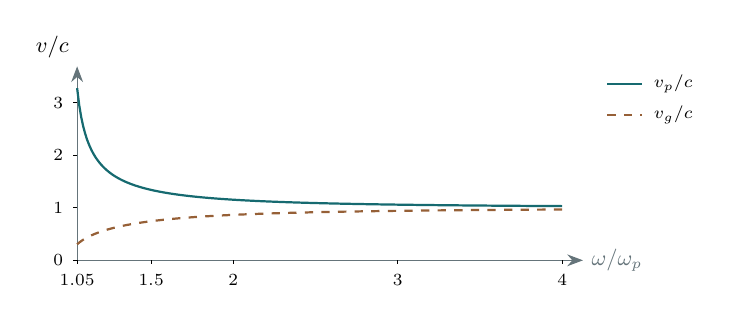
\begin{tikzpicture}[scale=.88,transform shape]
\draw[axis] (0,0.0)--(7.3,0.0) node[right] {$\omega/\omega_p$};
\draw[axis] (0,0)--(0,2.8);
\node[above left] at (0,2.8) {$v/c$};
\draw[thin] (0.000000,0.0)--(0.000000,-0.06);\node[below,font=\scriptsize] at (0.000000,-0.08) {$ 1.05 $};
\draw[thin] (1.067797,0.0)--(1.067797,-0.06);\node[below,font=\scriptsize] at (1.067797,-0.08) {$ 1.5 $};
\draw[thin] (2.254237,0.0)--(2.254237,-0.06);\node[below,font=\scriptsize] at (2.254237,-0.08) {$ 2 $};
\draw[thin] (4.627119,0.0)--(4.627119,-0.06);\node[below,font=\scriptsize] at (4.627119,-0.08) {$ 3 $};
\draw[thin] (7.000000,0.0)--(7.000000,-0.06);\node[below,font=\scriptsize] at (7.000000,-0.08) {$ 4 $};
\draw[thin] (0,0.000000)--(-.06,0.000000);\node[left,font=\scriptsize] at (-.08,0.000000) {$ 0 $};
\draw[thin] (0,0.757576)--(-.06,0.757576);\node[left,font=\scriptsize] at (-.08,0.757576) {$ 1 $};
\draw[thin] (0,1.515152)--(-.06,1.515152);\node[left,font=\scriptsize] at (-.08,1.515152) {$ 2 $};
\draw[thin] (0,2.272727)--(-.06,2.272727);\node[left,font=\scriptsize] at (-.08,2.272727) {$ 3 $};
\draw[thick,color=accent] plot coordinates {(0.0000000,2.4845826) (0.0291667,2.2453282) (0.0583333,2.0695686) (0.0875000,1.9337933) (0.1166667,1.8250859) (0.1458333,1.7356883) (0.1750000,1.6606246) (0.2041667,1.5965389) (0.2333333,1.5410752) (0.2625000,1.4925254) (0.2916667,1.4496170) (0.3208333,1.4113804) (0.3500000,1.3770623) (0.3791667,1.3460676) (0.4083333,1.3179190) (0.4375000,1.2922291) (0.4666667,1.2686793) (0.4958333,1.2470055) (0.5250000,1.2269862) (0.5541667,1.2084345) (0.5833333,1.1911912) (0.6125000,1.1751199) (0.6416667,1.1601029) (0.6708333,1.1460383) (0.7000000,1.1328369) (0.7291667,1.1204208) (0.7583333,1.1087212) (0.7875000,1.0976774) (0.8166667,1.0872355) (0.8458333,1.0773474) (0.8750000,1.0679700) (0.9041667,1.0590648) (0.9333333,1.0505970) (0.9625000,1.0425353) (0.9916667,1.0348513) (1.0208333,1.0275193) (1.0500000,1.0205157) (1.0791667,1.0138193) (1.1083333,1.0074104) (1.1375000,1.0012712) (1.1666667,0.9953852) (1.1958333,0.9897374) (1.2250000,0.9843138) (1.2541667,0.9791015) (1.2833333,0.9740887) (1.3125000,0.9692644) (1.3416667,0.9646184) (1.3708333,0.9601413) (1.4000000,0.9558241) (1.4291667,0.9516587) (1.4583333,0.9476375) (1.4875000,0.9437533) (1.5166667,0.9399994) (1.5458333,0.9363696) (1.5750000,0.9328580) (1.6041667,0.9294592) (1.6333333,0.9261679) (1.6625000,0.9229794) (1.6916667,0.9198890) (1.7208333,0.9168924) (1.7500000,0.9139857) (1.7791667,0.9111650) (1.8083333,0.9084266) (1.8375000,0.9057672) (1.8666667,0.9031836) (1.8958333,0.9006726) (1.9250000,0.8982315) (1.9541667,0.8958574) (1.9833333,0.8935477) (2.0125000,0.8913000) (2.0416667,0.8891120) (2.0708333,0.8869814) (2.1000000,0.8849061) (2.1291667,0.8828840) (2.1583333,0.8809133) (2.1875000,0.8789921) (2.2166667,0.8771187) (2.2458333,0.8752913) (2.2750000,0.8735085) (2.3041667,0.8717686) (2.3333333,0.8700703) (2.3625000,0.8684122) (2.3916667,0.8667928) (2.4208333,0.8652110) (2.4500000,0.8636655) (2.4791667,0.8621552) (2.5083333,0.8606789) (2.5375000,0.8592356) (2.5666667,0.8578243) (2.5958333,0.8564439) (2.6250000,0.8550935) (2.6541667,0.8537722) (2.6833333,0.8524792) (2.7125000,0.8512135) (2.7416667,0.8499745) (2.7708333,0.8487612) (2.8000000,0.8475730) (2.8291667,0.8464091) (2.8583333,0.8452689) (2.8875000,0.8441517) (2.9166667,0.8430568) (2.9458333,0.8419836) (2.9750000,0.8409316) (3.0041667,0.8399001) (3.0333333,0.8388886) (3.0625000,0.8378965) (3.0916667,0.8369234) (3.1208333,0.8359687) (3.1500000,0.8350320) (3.1791667,0.8341127) (3.2083333,0.8332105) (3.2375000,0.8323249) (3.2666667,0.8314555) (3.2958333,0.8306018) (3.3250000,0.8297635) (3.3541667,0.8289402) (3.3833333,0.8281316) (3.4125000,0.8273372) (3.4416667,0.8265567) (3.4708333,0.8257898) (3.5000000,0.8250361) (3.5291667,0.8242954) (3.5583333,0.8235674) (3.5875000,0.8228516) (3.6166667,0.8221479) (3.6458333,0.8214560) (3.6750000,0.8207756) (3.7041667,0.8201065) (3.7333333,0.8194483) (3.7625000,0.8188008) (3.7916667,0.8181639) (3.8208333,0.8175372) (3.8500000,0.8169205) (3.8791667,0.8163137) (3.9083333,0.8157165) (3.9375000,0.8151286) (3.9666667,0.8145500) (3.9958333,0.8139803) (4.0250000,0.8134194) (4.0541667,0.8128672) (4.0833333,0.8123234) (4.1125000,0.8117878) (4.1416667,0.8112604) (4.1708333,0.8107408) (4.2000000,0.8102290) (4.2291667,0.8097248) (4.2583333,0.8092281) (4.2875000,0.8087386) (4.3166667,0.8082563) (4.3458333,0.8077810) (4.3750000,0.8073126) (4.4041667,0.8068509) (4.4333333,0.8063958) (4.4625000,0.8059471) (4.4916667,0.8055048) (4.5208333,0.8050688) (4.5500000,0.8046388) (4.5791667,0.8042148) (4.6083333,0.8037967) (4.6375000,0.8033843) (4.6666667,0.8029776) (4.6958333,0.8025765) (4.7250000,0.8021807) (4.7541667,0.8017904) (4.7833333,0.8014053) (4.8125000,0.8010253) (4.8416667,0.8006504) (4.8708333,0.8002804) (4.9000000,0.7999153) (4.9291667,0.7995550) (4.9583333,0.7991994) (4.9875000,0.7988485) (5.0166667,0.7985020) (5.0458333,0.7981600) (5.0750000,0.7978224) (5.1041667,0.7974891) (5.1333333,0.7971601) (5.1625000,0.7968351) (5.1916667,0.7965143) (5.2208333,0.7961975) (5.2500000,0.7958846) (5.2791667,0.7955756) (5.3083333,0.7952704) (5.3375000,0.7949690) (5.3666667,0.7946712) (5.3958333,0.7943771) (5.4250000,0.7940866) (5.4541667,0.7937995) (5.4833333,0.7935159) (5.5125000,0.7932357) (5.5416667,0.7929588) (5.5708333,0.7926852) (5.6000000,0.7924149) (5.6291667,0.7921477) (5.6583333,0.7918837) (5.6875000,0.7916227) (5.7166667,0.7913648) (5.7458333,0.7911098) (5.7750000,0.7908578) (5.8041667,0.7906087) (5.8333333,0.7903624) (5.8625000,0.7901189) (5.8916667,0.7898782) (5.9208333,0.7896402) (5.9500000,0.7894049) (5.9791667,0.7891722) (6.0083333,0.7889421) (6.0375000,0.7887146) (6.0666667,0.7884895) (6.0958333,0.7882670) (6.1250000,0.7880469) (6.1541667,0.7878292) (6.1833333,0.7876138) (6.2125000,0.7874008) (6.2416667,0.7871901) (6.2708333,0.7869817) (6.3000000,0.7867755) (6.3291667,0.7865715) (6.3583333,0.7863697) (6.3875000,0.7861700) (6.4166667,0.7859724) (6.4458333,0.7857769) (6.4750000,0.7855835) (6.5041667,0.7853920) (6.5333333,0.7852026) (6.5625000,0.7850151) (6.5916667,0.7848296) (6.6208333,0.7846459) (6.6500000,0.7844642) (6.6791667,0.7842843) (6.7083333,0.7841062) (6.7375000,0.7839300) (6.7666667,0.7837555) (6.7958333,0.7835827) (6.8250000,0.7834117) (6.8541667,0.7832425) (6.8833333,0.7830749) (6.9125000,0.7829089) (6.9416667,0.7827446) (6.9708333,0.7825820) (7.0000000,0.7824209)};
\draw[thick,color=accent] (7.65,2.55)--(8.15,2.55);\node[right,font=\scriptsize] at (8.2,2.55) {$v_p/c$};
\draw[thick,dashed,color=warm] plot coordinates {(0.0000000,0.2309929) (0.0291667,0.2556067) (0.0583333,0.2773143) (0.0875000,0.2967851) (0.1166667,0.3144625) (0.1458333,0.3306590) (0.1750000,0.3456055) (0.2041667,0.3594783) (0.2333333,0.3724160) (0.2625000,0.3845302) (0.2916667,0.3959122) (0.3208333,0.4066381) (0.3500000,0.4167720) (0.3791667,0.4263686) (0.4083333,0.4354752) (0.4375000,0.4441326) (0.4666667,0.4523767) (0.4958333,0.4602394) (0.5250000,0.4677485) (0.5541667,0.4749294) (0.5833333,0.4818043) (0.6125000,0.4883936) (0.6416667,0.4947156) (0.6708333,0.5007870) (0.7000000,0.5066228) (0.7291667,0.5122371) (0.7583333,0.5176423) (0.7875000,0.5228504) (0.8166667,0.5278719) (0.8458333,0.5327168) (0.8750000,0.5373943) (0.9041667,0.5419131) (0.9333333,0.5462809) (0.9625000,0.5505051) (0.9916667,0.5545927) (1.0208333,0.5585501) (1.0500000,0.5623833) (1.0791667,0.5660980) (1.1083333,0.5696993) (1.1375000,0.5731924) (1.1666667,0.5765818) (1.1958333,0.5798720) (1.2250000,0.5830671) (1.2541667,0.5861711) (1.2833333,0.5891876) (1.3125000,0.5921202) (1.3416667,0.5949721) (1.3708333,0.5977465) (1.4000000,0.6004463) (1.4291667,0.6030744) (1.4583333,0.6056335) (1.4875000,0.6081261) (1.5166667,0.6105547) (1.5458333,0.6129215) (1.5750000,0.6152287) (1.6041667,0.6174785) (1.6333333,0.6196728) (1.6625000,0.6218135) (1.6916667,0.6239025) (1.7208333,0.6259415) (1.7500000,0.6279322) (1.7791667,0.6298761) (1.8083333,0.6317748) (1.8375000,0.6336297) (1.8666667,0.6354423) (1.8958333,0.6372138) (1.9250000,0.6389456) (1.9541667,0.6406389) (1.9833333,0.6422948) (2.0125000,0.6439145) (2.0416667,0.6454991) (2.0708333,0.6470497) (2.1000000,0.6485672) (2.1291667,0.6500526) (2.1583333,0.6515068) (2.1875000,0.6529308) (2.2166667,0.6543254) (2.2458333,0.6556914) (2.2750000,0.6570297) (2.3041667,0.6583410) (2.3333333,0.6596260) (2.3625000,0.6608855) (2.3916667,0.6621202) (2.4208333,0.6633307) (2.4500000,0.6645177) (2.4791667,0.6656818) (2.5083333,0.6668236) (2.5375000,0.6679437) (2.5666667,0.6690426) (2.5958333,0.6701210) (2.6250000,0.6711793) (2.6541667,0.6722180) (2.6833333,0.6732376) (2.7125000,0.6742386) (2.7416667,0.6752215) (2.7708333,0.6761867) (2.8000000,0.6771346) (2.8291667,0.6780657) (2.8583333,0.6789804) (2.8875000,0.6798790) (2.9166667,0.6807620) (2.9458333,0.6816297) (2.9750000,0.6824824) (3.0041667,0.6833206) (3.0333333,0.6841445) (3.0625000,0.6849545) (3.0916667,0.6857510) (3.1208333,0.6865341) (3.1500000,0.6873042) (3.1791667,0.6880617) (3.2083333,0.6888067) (3.2375000,0.6895396) (3.2666667,0.6902607) (3.2958333,0.6909701) (3.3250000,0.6916682) (3.3541667,0.6923551) (3.3833333,0.6930312) (3.4125000,0.6936967) (3.4416667,0.6943517) (3.4708333,0.6949965) (3.5000000,0.6956314) (3.5291667,0.6962565) (3.5583333,0.6968720) (3.5875000,0.6974782) (3.6166667,0.6980751) (3.6458333,0.6986631) (3.6750000,0.6992423) (3.7041667,0.6998128) (3.7333333,0.7003749) (3.7625000,0.7009287) (3.7916667,0.7014744) (3.8208333,0.7020121) (3.8500000,0.7025420) (3.8791667,0.7030643) (3.9083333,0.7035791) (3.9375000,0.7040865) (3.9666667,0.7045866) (3.9958333,0.7050797) (4.0250000,0.7055659) (4.0541667,0.7060453) (4.0833333,0.7065179) (4.1125000,0.7069840) (4.1416667,0.7074437) (4.1708333,0.7078970) (4.2000000,0.7083442) (4.2291667,0.7087853) (4.2583333,0.7092203) (4.2875000,0.7096496) (4.3166667,0.7100730) (4.3458333,0.7104909) (4.3750000,0.7109031) (4.4041667,0.7113099) (4.4333333,0.7117114) (4.4625000,0.7121075) (4.4916667,0.7124986) (4.5208333,0.7128845) (4.5500000,0.7132654) (4.5791667,0.7136415) (4.6083333,0.7140127) (4.6375000,0.7143792) (4.6666667,0.7147410) (4.6958333,0.7150983) (4.7250000,0.7154510) (4.7541667,0.7157993) (4.7833333,0.7161433) (4.8125000,0.7164830) (4.8416667,0.7168186) (4.8708333,0.7171499) (4.9000000,0.7174772) (4.9291667,0.7178005) (4.9583333,0.7181199) (4.9875000,0.7184354) (5.0166667,0.7187471) (5.0458333,0.7190551) (5.0750000,0.7193594) (5.1041667,0.7196600) (5.1333333,0.7199571) (5.1625000,0.7202507) (5.1916667,0.7205408) (5.2208333,0.7208275) (5.2500000,0.7211109) (5.2791667,0.7213909) (5.3083333,0.7216678) (5.3375000,0.7219414) (5.3666667,0.7222119) (5.3958333,0.7224793) (5.4250000,0.7227437) (5.4541667,0.7230050) (5.4833333,0.7232634) (5.5125000,0.7235189) (5.5416667,0.7237715) (5.5708333,0.7240213) (5.6000000,0.7242683) (5.6291667,0.7245126) (5.6583333,0.7247542) (5.6875000,0.7249931) (5.7166667,0.7252294) (5.7458333,0.7254631) (5.7750000,0.7256943) (5.8041667,0.7259230) (5.8333333,0.7261492) (5.8625000,0.7263729) (5.8916667,0.7265943) (5.9208333,0.7268133) (5.9500000,0.7270300) (5.9791667,0.7272444) (6.0083333,0.7274565) (6.0375000,0.7276663) (6.0666667,0.7278740) (6.0958333,0.7280795) (6.1250000,0.7282829) (6.1541667,0.7284841) (6.1833333,0.7286833) (6.2125000,0.7288804) (6.2416667,0.7290755) (6.2708333,0.7292686) (6.3000000,0.7294597) (6.3291667,0.7296489) (6.3583333,0.7298362) (6.3875000,0.7300215) (6.4166667,0.7302050) (6.4458333,0.7303867) (6.4750000,0.7305666) (6.5041667,0.7307447) (6.5333333,0.7309210) (6.5625000,0.7310955) (6.5916667,0.7312684) (6.6208333,0.7314395) (6.6500000,0.7316090) (6.6791667,0.7317768) (6.7083333,0.7319430) (6.7375000,0.7321075) (6.7666667,0.7322705) (6.7958333,0.7324319) (6.8250000,0.7325918) (6.8541667,0.7327501) (6.8833333,0.7329070) (6.9125000,0.7330623) (6.9416667,0.7332162) (6.9708333,0.7333686) (7.0000000,0.7335196)};
\draw[thick,dashed,color=warm] (7.65,2.0999999999999996)--(8.15,2.0999999999999996);\node[right,font=\scriptsize] at (8.2,2.0999999999999996) {$v_g/c$};
\end{tikzpicture}
\figcaption{解图光5.4B\quad 同一传播频率下相速和群速的乘积为$c^2$}
\end{minipage}\end{center}
解图光5.4D改变电子数密度，显示$K\propto N$、$\omega_p\propto\sqrt N$。等式$v_pv_g=c^2$具体对应$\omega^2=c^2k^2+\omega_p^2$这一平方型色散。恢复非零束缚频率或阻尼后，按相应的复频率响应求导，速度关系随之改变。铜在22.4nm附近的真实响应还包含这些束缚与吸收过程，而上面给出的$.10\,\mathrm{nm}$数值使用全电子高频近似。
\begin{center}\begin{minipage}{.98\linewidth}\centering
\begin{tikzpicture}[scale=.88,transform shape]
\draw[axis] (0,0.0)--(7.3,0.0) node[right] {$N^\prime/N$};
\draw[axis] (0,0)--(0,2.8);
\node[above left] at (0,2.8) {$\text{参数比例}$};
\draw[thin] (0.000000,0.0)--(0.000000,-0.06);\node[below,font=\scriptsize] at (0.000000,-0.08) {$ 0.5 $};
\draw[thin] (2.333333,0.0)--(2.333333,-0.06);\node[below,font=\scriptsize] at (2.333333,-0.08) {$ 1 $};
\draw[thin] (4.666667,0.0)--(4.666667,-0.06);\node[below,font=\scriptsize] at (4.666667,-0.08) {$ 1.5 $};
\draw[thin] (7.000000,0.0)--(7.000000,-0.06);\node[below,font=\scriptsize] at (7.000000,-0.08) {$ 2 $};
\draw[thin] (0,0.000000)--(-.06,0.000000);\node[left,font=\scriptsize] at (-.08,0.000000) {$ 0 $};
\draw[thin] (0,1.190476)--(-.06,1.190476);\node[left,font=\scriptsize] at (-.08,1.190476) {$ 1 $};
\draw[thin] (0,1.683588)--(-.06,1.683588);\node[left,font=\scriptsize] at (-.08,1.683588) {$ 1.41421 $};
\draw[thin] (0,2.380952)--(-.06,2.380952);\node[left,font=\scriptsize] at (-.08,2.380952) {$ 2 $};
\draw[thick,color=accent] plot coordinates {(0.0000000,0.5952381) (0.0291667,0.6026786) (0.0583333,0.6101190) (0.0875000,0.6175595) (0.1166667,0.6250000) (0.1458333,0.6324405) (0.1750000,0.6398810) (0.2041667,0.6473214) (0.2333333,0.6547619) (0.2625000,0.6622024) (0.2916667,0.6696429) (0.3208333,0.6770833) (0.3500000,0.6845238) (0.3791667,0.6919643) (0.4083333,0.6994048) (0.4375000,0.7068452) (0.4666667,0.7142857) (0.4958333,0.7217262) (0.5250000,0.7291667) (0.5541667,0.7366071) (0.5833333,0.7440476) (0.6125000,0.7514881) (0.6416667,0.7589286) (0.6708333,0.7663690) (0.7000000,0.7738095) (0.7291667,0.7812500) (0.7583333,0.7886905) (0.7875000,0.7961310) (0.8166667,0.8035714) (0.8458333,0.8110119) (0.8750000,0.8184524) (0.9041667,0.8258929) (0.9333333,0.8333333) (0.9625000,0.8407738) (0.9916667,0.8482143) (1.0208333,0.8556548) (1.0500000,0.8630952) (1.0791667,0.8705357) (1.1083333,0.8779762) (1.1375000,0.8854167) (1.1666667,0.8928571) (1.1958333,0.9002976) (1.2250000,0.9077381) (1.2541667,0.9151786) (1.2833333,0.9226190) (1.3125000,0.9300595) (1.3416667,0.9375000) (1.3708333,0.9449405) (1.4000000,0.9523810) (1.4291667,0.9598214) (1.4583333,0.9672619) (1.4875000,0.9747024) (1.5166667,0.9821429) (1.5458333,0.9895833) (1.5750000,0.9970238) (1.6041667,1.0044643) (1.6333333,1.0119048) (1.6625000,1.0193452) (1.6916667,1.0267857) (1.7208333,1.0342262) (1.7500000,1.0416667) (1.7791667,1.0491071) (1.8083333,1.0565476) (1.8375000,1.0639881) (1.8666667,1.0714286) (1.8958333,1.0788690) (1.9250000,1.0863095) (1.9541667,1.0937500) (1.9833333,1.1011905) (2.0125000,1.1086310) (2.0416667,1.1160714) (2.0708333,1.1235119) (2.1000000,1.1309524) (2.1291667,1.1383929) (2.1583333,1.1458333) (2.1875000,1.1532738) (2.2166667,1.1607143) (2.2458333,1.1681548) (2.2750000,1.1755952) (2.3041667,1.1830357) (2.3333333,1.1904762) (2.3625000,1.1979167) (2.3916667,1.2053571) (2.4208333,1.2127976) (2.4500000,1.2202381) (2.4791667,1.2276786) (2.5083333,1.2351190) (2.5375000,1.2425595) (2.5666667,1.2500000) (2.5958333,1.2574405) (2.6250000,1.2648810) (2.6541667,1.2723214) (2.6833333,1.2797619) (2.7125000,1.2872024) (2.7416667,1.2946429) (2.7708333,1.3020833) (2.8000000,1.3095238) (2.8291667,1.3169643) (2.8583333,1.3244048) (2.8875000,1.3318452) (2.9166667,1.3392857) (2.9458333,1.3467262) (2.9750000,1.3541667) (3.0041667,1.3616071) (3.0333333,1.3690476) (3.0625000,1.3764881) (3.0916667,1.3839286) (3.1208333,1.3913690) (3.1500000,1.3988095) (3.1791667,1.4062500) (3.2083333,1.4136905) (3.2375000,1.4211310) (3.2666667,1.4285714) (3.2958333,1.4360119) (3.3250000,1.4434524) (3.3541667,1.4508929) (3.3833333,1.4583333) (3.4125000,1.4657738) (3.4416667,1.4732143) (3.4708333,1.4806548) (3.5000000,1.4880952) (3.5291667,1.4955357) (3.5583333,1.5029762) (3.5875000,1.5104167) (3.6166667,1.5178571) (3.6458333,1.5252976) (3.6750000,1.5327381) (3.7041667,1.5401786) (3.7333333,1.5476190) (3.7625000,1.5550595) (3.7916667,1.5625000) (3.8208333,1.5699405) (3.8500000,1.5773810) (3.8791667,1.5848214) (3.9083333,1.5922619) (3.9375000,1.5997024) (3.9666667,1.6071429) (3.9958333,1.6145833) (4.0250000,1.6220238) (4.0541667,1.6294643) (4.0833333,1.6369048) (4.1125000,1.6443452) (4.1416667,1.6517857) (4.1708333,1.6592262) (4.2000000,1.6666667) (4.2291667,1.6741071) (4.2583333,1.6815476) (4.2875000,1.6889881) (4.3166667,1.6964286) (4.3458333,1.7038690) (4.3750000,1.7113095) (4.4041667,1.7187500) (4.4333333,1.7261905) (4.4625000,1.7336310) (4.4916667,1.7410714) (4.5208333,1.7485119) (4.5500000,1.7559524) (4.5791667,1.7633929) (4.6083333,1.7708333) (4.6375000,1.7782738) (4.6666667,1.7857143) (4.6958333,1.7931548) (4.7250000,1.8005952) (4.7541667,1.8080357) (4.7833333,1.8154762) (4.8125000,1.8229167) (4.8416667,1.8303571) (4.8708333,1.8377976) (4.9000000,1.8452381) (4.9291667,1.8526786) (4.9583333,1.8601190) (4.9875000,1.8675595) (5.0166667,1.8750000) (5.0458333,1.8824405) (5.0750000,1.8898810) (5.1041667,1.8973214) (5.1333333,1.9047619) (5.1625000,1.9122024) (5.1916667,1.9196429) (5.2208333,1.9270833) (5.2500000,1.9345238) (5.2791667,1.9419643) (5.3083333,1.9494048) (5.3375000,1.9568452) (5.3666667,1.9642857) (5.3958333,1.9717262) (5.4250000,1.9791667) (5.4541667,1.9866071) (5.4833333,1.9940476) (5.5125000,2.0014881) (5.5416667,2.0089286) (5.5708333,2.0163690) (5.6000000,2.0238095) (5.6291667,2.0312500) (5.6583333,2.0386905) (5.6875000,2.0461310) (5.7166667,2.0535714) (5.7458333,2.0610119) (5.7750000,2.0684524) (5.8041667,2.0758929) (5.8333333,2.0833333) (5.8625000,2.0907738) (5.8916667,2.0982143) (5.9208333,2.1056548) (5.9500000,2.1130952) (5.9791667,2.1205357) (6.0083333,2.1279762) (6.0375000,2.1354167) (6.0666667,2.1428571) (6.0958333,2.1502976) (6.1250000,2.1577381) (6.1541667,2.1651786) (6.1833333,2.1726190) (6.2125000,2.1800595) (6.2416667,2.1875000) (6.2708333,2.1949405) (6.3000000,2.2023810) (6.3291667,2.2098214) (6.3583333,2.2172619) (6.3875000,2.2247024) (6.4166667,2.2321429) (6.4458333,2.2395833) (6.4750000,2.2470238) (6.5041667,2.2544643) (6.5333333,2.2619048) (6.5625000,2.2693452) (6.5916667,2.2767857) (6.6208333,2.2842262) (6.6500000,2.2916667) (6.6791667,2.2991071) (6.7083333,2.3065476) (6.7375000,2.3139881) (6.7666667,2.3214286) (6.7958333,2.3288690) (6.8250000,2.3363095) (6.8541667,2.3437500) (6.8833333,2.3511905) (6.9125000,2.3586310) (6.9416667,2.3660714) (6.9708333,2.3735119) (7.0000000,2.3809524)};
\draw[thick,color=accent] (7.65,2.55)--(8.15,2.55);\node[right,font=\scriptsize] at (8.2,2.55) {$K^\prime/K$};
\draw[thick,dashed,color=warm] plot coordinates {(0.0000000,0.8417938) (0.0291667,0.8470387) (0.0583333,0.8522513) (0.0875000,0.8574322) (0.1166667,0.8625819) (0.1458333,0.8677012) (0.1750000,0.8727904) (0.2041667,0.8778501) (0.2333333,0.8828808) (0.2625000,0.8878830) (0.2916667,0.8928571) (0.3208333,0.8978038) (0.3500000,0.9027233) (0.3791667,0.9076161) (0.4083333,0.9124827) (0.4375000,0.9173235) (0.4666667,0.9221389) (0.4958333,0.9269293) (0.5250000,0.9316950) (0.5541667,0.9364365) (0.5833333,0.9411541) (0.6125000,0.9458481) (0.6416667,0.9505190) (0.6708333,0.9551671) (0.7000000,0.9597926) (0.7291667,0.9643959) (0.7583333,0.9689774) (0.7875000,0.9735373) (0.8166667,0.9780760) (0.8458333,0.9825937) (0.8750000,0.9870907) (0.9041667,0.9915673) (0.9333333,0.9960238) (0.9625000,1.0004605) (0.9916667,1.0048776) (1.0208333,1.0092753) (1.0500000,1.0136540) (1.0791667,1.0180138) (1.1083333,1.0223550) (1.1375000,1.0266779) (1.1666667,1.0309826) (1.1958333,1.0352695) (1.2250000,1.0395386) (1.2541667,1.0437904) (1.2833333,1.0480248) (1.3125000,1.0522422) (1.3416667,1.0564428) (1.3708333,1.0606268) (1.4000000,1.0647943) (1.4291667,1.0689455) (1.4583333,1.0730807) (1.4875000,1.0772001) (1.5166667,1.0813037) (1.5458333,1.0853918) (1.5750000,1.0894646) (1.6041667,1.0935222) (1.6333333,1.0975648) (1.6625000,1.1015926) (1.6916667,1.1056057) (1.7208333,1.1096043) (1.7500000,1.1135885) (1.7791667,1.1175585) (1.8083333,1.1215145) (1.8375000,1.1254566) (1.8666667,1.1293849) (1.8958333,1.1332996) (1.9250000,1.1372008) (1.9541667,1.1410887) (1.9833333,1.1449633) (2.0125000,1.1488249) (2.0416667,1.1526736) (2.0708333,1.1565095) (2.1000000,1.1603327) (2.1291667,1.1641433) (2.1583333,1.1679415) (2.1875000,1.1717274) (2.2166667,1.1755011) (2.2458333,1.1792627) (2.2750000,1.1830123) (2.3041667,1.1867501) (2.3333333,1.1904762) (2.3625000,1.1941906) (2.3916667,1.1978936) (2.4208333,1.2015851) (2.4500000,1.2052653) (2.4791667,1.2089343) (2.5083333,1.2125922) (2.5375000,1.2162391) (2.5666667,1.2198751) (2.5958333,1.2235003) (2.6250000,1.2271148) (2.6541667,1.2307186) (2.6833333,1.2343120) (2.7125000,1.2378949) (2.7416667,1.2414675) (2.7708333,1.2450298) (2.8000000,1.2485820) (2.8291667,1.2521240) (2.8583333,1.2556561) (2.8875000,1.2591783) (2.9166667,1.2626907) (2.9458333,1.2661933) (2.9750000,1.2696863) (3.0041667,1.2731696) (3.0333333,1.2766435) (3.0625000,1.2801079) (3.0916667,1.2835630) (3.1208333,1.2870088) (3.1500000,1.2904454) (3.1791667,1.2938729) (3.2083333,1.2972914) (3.2375000,1.3007008) (3.2666667,1.3041013) (3.2958333,1.3074930) (3.3250000,1.3108759) (3.3541667,1.3142501) (3.3833333,1.3176157) (3.4125000,1.3209727) (3.4416667,1.3243212) (3.4708333,1.3276612) (3.5000000,1.3309928) (3.5291667,1.3343162) (3.5583333,1.3376313) (3.5875000,1.3409381) (3.6166667,1.3442369) (3.6458333,1.3475276) (3.6750000,1.3508102) (3.7041667,1.3540849) (3.7333333,1.3573517) (3.7625000,1.3606106) (3.7916667,1.3638618) (3.8208333,1.3671052) (3.8500000,1.3703410) (3.8791667,1.3735691) (3.9083333,1.3767897) (3.9375000,1.3800028) (3.9666667,1.3832083) (3.9958333,1.3864065) (4.0250000,1.3895973) (4.0541667,1.3927808) (4.0833333,1.3959571) (4.1125000,1.3991261) (4.1416667,1.4022880) (4.1708333,1.4054427) (4.2000000,1.4085904) (4.2291667,1.4117311) (4.2583333,1.4148648) (4.2875000,1.4179916) (4.3166667,1.4211115) (4.3458333,1.4242245) (4.3750000,1.4273308) (4.4041667,1.4304303) (4.4333333,1.4335232) (4.4625000,1.4366093) (4.4916667,1.4396889) (4.5208333,1.4427619) (4.5500000,1.4458283) (4.5791667,1.4488883) (4.6083333,1.4519418) (4.6375000,1.4549889) (4.6666667,1.4580296) (4.6958333,1.4610640) (4.7250000,1.4640921) (4.7541667,1.4671140) (4.7833333,1.4701296) (4.8125000,1.4731391) (4.8416667,1.4761425) (4.8708333,1.4791397) (4.9000000,1.4821309) (4.9291667,1.4851161) (4.9583333,1.4880952) (4.9875000,1.4910685) (5.0166667,1.4940358) (5.0458333,1.4969972) (5.0750000,1.4999528) (5.1041667,1.5029025) (5.1333333,1.5058465) (5.1625000,1.5087847) (5.1916667,1.5117173) (5.2208333,1.5146441) (5.2500000,1.5175653) (5.2791667,1.5204809) (5.3083333,1.5233909) (5.3375000,1.5262954) (5.3666667,1.5291944) (5.3958333,1.5320878) (5.4250000,1.5349758) (5.4541667,1.5378584) (5.4833333,1.5407356) (5.5125000,1.5436074) (5.5416667,1.5464739) (5.5708333,1.5493351) (5.6000000,1.5521910) (5.6291667,1.5550417) (5.6583333,1.5578872) (5.6875000,1.5607275) (5.7166667,1.5635626) (5.7458333,1.5663925) (5.7750000,1.5692174) (5.8041667,1.5720372) (5.8333333,1.5748520) (5.8625000,1.5776617) (5.8916667,1.5804664) (5.9208333,1.5832662) (5.9500000,1.5860610) (5.9791667,1.5888509) (6.0083333,1.5916359) (6.0375000,1.5944161) (6.0666667,1.5971914) (6.0958333,1.5999619) (6.1250000,1.6027276) (6.1541667,1.6054886) (6.1833333,1.6082448) (6.2125000,1.6109963) (6.2416667,1.6137431) (6.2708333,1.6164852) (6.3000000,1.6192227) (6.3291667,1.6219555) (6.3583333,1.6246838) (6.3875000,1.6274075) (6.4166667,1.6301267) (6.4458333,1.6328413) (6.4750000,1.6355514) (6.5041667,1.6382570) (6.5333333,1.6409582) (6.5625000,1.6436549) (6.5916667,1.6463472) (6.6208333,1.6490351) (6.6500000,1.6517187) (6.6791667,1.6543979) (6.7083333,1.6570727) (6.7375000,1.6597433) (6.7666667,1.6624095) (6.7958333,1.6650715) (6.8250000,1.6677293) (6.8541667,1.6703828) (6.8833333,1.6730321) (6.9125000,1.6756772) (6.9416667,1.6783181) (6.9708333,1.6809549) (7.0000000,1.6835876)};
\draw[thick,dashed,color=warm] (7.65,2.0999999999999996)--(8.15,2.0999999999999996);\node[right,font=\scriptsize] at (8.2,2.0999999999999996) {$\omega_p^\prime/\omega_p$};
\end{tikzpicture}
\figcaption{解图光5.4D\quad 电子数密度对K与特征频率的不同幂次作用}
\end{minipage}\end{center}


\Needspace{8\baselineskip}

\pdfbookmark[3]{关键洞察}{q4-h5}

\subsection*{关键洞察}

速度乘积由平方型色散的代数结构固定。把非零束缚频率保留下来，会在$n n_g$中增加相应项；因而该乘积关系与所采用的频率响应相连。

\Needspace{8\baselineskip}

\pdfbookmark[3]{易错点}{q4-h6}

\subsection*{易错点}

\begin{itemize}
\item 高频极化的负号取自$\omega_j^2-\omega^2$分母，电荷在响应中以平方出现。
\item 用总电子计数求高频$K$，价电子计数对应另一自由电子近似及频率范围。
\item 相位面、窄带能量包络和信号前沿是不同传播对象，本题分别由$1/n$、$n$和完整因果响应描述。
\item 求实相速与群速的乘积时，使用$\omega>\omega_p$的传播分支。
\end{itemize}

\Needspace{8\baselineskip}

\pdfbookmark[3]{课堂讲解建议}{q4-h7}

\subsection*{课堂讲解建议}

先让学生画电子位移与电场的相位关系，由两次负电荷因子得出负极化。接着计算每立方米原子数和全部电子数，说明计数条件。A图选定一个工作点后再画两斜率，B图随频率移动工作点。最后改变电子数密度与束缚频率，分别观察参数尺度和速度乘积怎样变化。

\Needspace{8\baselineskip}

\pdfbookmark[3]{变式训练}{q4-h8}

\subsection*{变式训练}

\begin{enumerate}
\item \textbf{电子数密度加倍。}频率和单电子质量、电荷不变，求$K,\omega_p$及$.10\,\mathrm{nm}$处折射率偏离的变化。

由$K\propto N$、$\omega_p^2\propto N$，有$K'=2K$、$\omega'_p=\sqrt2\omega_p$。同一波长的$n'=\sqrt{1-2K\lambda_0^2}$，小偏离满足$1-n'\simeq K\lambda_0^2$，为起初一阶值的两倍。变图光5.4V1同时画$K'/K$和$\omega'_p/\omega_p$的密度比例，在$N'/N=2$处分别为2与$\sqrt2$。
\begin{center}\begin{minipage}{.98\linewidth}\centering
\begin{tikzpicture}[scale=.88,transform shape]
\draw[axis] (0,0.0)--(7.3,0.0) node[right] {$N^\prime/N$};
\draw[axis] (0,0)--(0,2.8);
\node[above left] at (0,2.8) {$\text{参数比例}$};
\draw[thin] (0.000000,0.0)--(0.000000,-0.06);\node[below,font=\scriptsize] at (0.000000,-0.08) {$ 0.5 $};
\draw[thin] (2.333333,0.0)--(2.333333,-0.06);\node[below,font=\scriptsize] at (2.333333,-0.08) {$ 1 $};
\draw[thin] (4.666667,0.0)--(4.666667,-0.06);\node[below,font=\scriptsize] at (4.666667,-0.08) {$ 1.5 $};
\draw[thin] (7.000000,0.0)--(7.000000,-0.06);\node[below,font=\scriptsize] at (7.000000,-0.08) {$ 2 $};
\draw[thin] (0,0.000000)--(-.06,0.000000);\node[left,font=\scriptsize] at (-.08,0.000000) {$ 0 $};
\draw[thin] (0,1.190476)--(-.06,1.190476);\node[left,font=\scriptsize] at (-.08,1.190476) {$ 1 $};
\draw[thin] (0,1.683588)--(-.06,1.683588);\node[left,font=\scriptsize] at (-.08,1.683588) {$ 1.41421 $};
\draw[thin] (0,2.380952)--(-.06,2.380952);\node[left,font=\scriptsize] at (-.08,2.380952) {$ 2 $};
\draw[thick,color=accent] plot coordinates {(0.0000000,0.5952381) (0.0291667,0.6026786) (0.0583333,0.6101190) (0.0875000,0.6175595) (0.1166667,0.6250000) (0.1458333,0.6324405) (0.1750000,0.6398810) (0.2041667,0.6473214) (0.2333333,0.6547619) (0.2625000,0.6622024) (0.2916667,0.6696429) (0.3208333,0.6770833) (0.3500000,0.6845238) (0.3791667,0.6919643) (0.4083333,0.6994048) (0.4375000,0.7068452) (0.4666667,0.7142857) (0.4958333,0.7217262) (0.5250000,0.7291667) (0.5541667,0.7366071) (0.5833333,0.7440476) (0.6125000,0.7514881) (0.6416667,0.7589286) (0.6708333,0.7663690) (0.7000000,0.7738095) (0.7291667,0.7812500) (0.7583333,0.7886905) (0.7875000,0.7961310) (0.8166667,0.8035714) (0.8458333,0.8110119) (0.8750000,0.8184524) (0.9041667,0.8258929) (0.9333333,0.8333333) (0.9625000,0.8407738) (0.9916667,0.8482143) (1.0208333,0.8556548) (1.0500000,0.8630952) (1.0791667,0.8705357) (1.1083333,0.8779762) (1.1375000,0.8854167) (1.1666667,0.8928571) (1.1958333,0.9002976) (1.2250000,0.9077381) (1.2541667,0.9151786) (1.2833333,0.9226190) (1.3125000,0.9300595) (1.3416667,0.9375000) (1.3708333,0.9449405) (1.4000000,0.9523810) (1.4291667,0.9598214) (1.4583333,0.9672619) (1.4875000,0.9747024) (1.5166667,0.9821429) (1.5458333,0.9895833) (1.5750000,0.9970238) (1.6041667,1.0044643) (1.6333333,1.0119048) (1.6625000,1.0193452) (1.6916667,1.0267857) (1.7208333,1.0342262) (1.7500000,1.0416667) (1.7791667,1.0491071) (1.8083333,1.0565476) (1.8375000,1.0639881) (1.8666667,1.0714286) (1.8958333,1.0788690) (1.9250000,1.0863095) (1.9541667,1.0937500) (1.9833333,1.1011905) (2.0125000,1.1086310) (2.0416667,1.1160714) (2.0708333,1.1235119) (2.1000000,1.1309524) (2.1291667,1.1383929) (2.1583333,1.1458333) (2.1875000,1.1532738) (2.2166667,1.1607143) (2.2458333,1.1681548) (2.2750000,1.1755952) (2.3041667,1.1830357) (2.3333333,1.1904762) (2.3625000,1.1979167) (2.3916667,1.2053571) (2.4208333,1.2127976) (2.4500000,1.2202381) (2.4791667,1.2276786) (2.5083333,1.2351190) (2.5375000,1.2425595) (2.5666667,1.2500000) (2.5958333,1.2574405) (2.6250000,1.2648810) (2.6541667,1.2723214) (2.6833333,1.2797619) (2.7125000,1.2872024) (2.7416667,1.2946429) (2.7708333,1.3020833) (2.8000000,1.3095238) (2.8291667,1.3169643) (2.8583333,1.3244048) (2.8875000,1.3318452) (2.9166667,1.3392857) (2.9458333,1.3467262) (2.9750000,1.3541667) (3.0041667,1.3616071) (3.0333333,1.3690476) (3.0625000,1.3764881) (3.0916667,1.3839286) (3.1208333,1.3913690) (3.1500000,1.3988095) (3.1791667,1.4062500) (3.2083333,1.4136905) (3.2375000,1.4211310) (3.2666667,1.4285714) (3.2958333,1.4360119) (3.3250000,1.4434524) (3.3541667,1.4508929) (3.3833333,1.4583333) (3.4125000,1.4657738) (3.4416667,1.4732143) (3.4708333,1.4806548) (3.5000000,1.4880952) (3.5291667,1.4955357) (3.5583333,1.5029762) (3.5875000,1.5104167) (3.6166667,1.5178571) (3.6458333,1.5252976) (3.6750000,1.5327381) (3.7041667,1.5401786) (3.7333333,1.5476190) (3.7625000,1.5550595) (3.7916667,1.5625000) (3.8208333,1.5699405) (3.8500000,1.5773810) (3.8791667,1.5848214) (3.9083333,1.5922619) (3.9375000,1.5997024) (3.9666667,1.6071429) (3.9958333,1.6145833) (4.0250000,1.6220238) (4.0541667,1.6294643) (4.0833333,1.6369048) (4.1125000,1.6443452) (4.1416667,1.6517857) (4.1708333,1.6592262) (4.2000000,1.6666667) (4.2291667,1.6741071) (4.2583333,1.6815476) (4.2875000,1.6889881) (4.3166667,1.6964286) (4.3458333,1.7038690) (4.3750000,1.7113095) (4.4041667,1.7187500) (4.4333333,1.7261905) (4.4625000,1.7336310) (4.4916667,1.7410714) (4.5208333,1.7485119) (4.5500000,1.7559524) (4.5791667,1.7633929) (4.6083333,1.7708333) (4.6375000,1.7782738) (4.6666667,1.7857143) (4.6958333,1.7931548) (4.7250000,1.8005952) (4.7541667,1.8080357) (4.7833333,1.8154762) (4.8125000,1.8229167) (4.8416667,1.8303571) (4.8708333,1.8377976) (4.9000000,1.8452381) (4.9291667,1.8526786) (4.9583333,1.8601190) (4.9875000,1.8675595) (5.0166667,1.8750000) (5.0458333,1.8824405) (5.0750000,1.8898810) (5.1041667,1.8973214) (5.1333333,1.9047619) (5.1625000,1.9122024) (5.1916667,1.9196429) (5.2208333,1.9270833) (5.2500000,1.9345238) (5.2791667,1.9419643) (5.3083333,1.9494048) (5.3375000,1.9568452) (5.3666667,1.9642857) (5.3958333,1.9717262) (5.4250000,1.9791667) (5.4541667,1.9866071) (5.4833333,1.9940476) (5.5125000,2.0014881) (5.5416667,2.0089286) (5.5708333,2.0163690) (5.6000000,2.0238095) (5.6291667,2.0312500) (5.6583333,2.0386905) (5.6875000,2.0461310) (5.7166667,2.0535714) (5.7458333,2.0610119) (5.7750000,2.0684524) (5.8041667,2.0758929) (5.8333333,2.0833333) (5.8625000,2.0907738) (5.8916667,2.0982143) (5.9208333,2.1056548) (5.9500000,2.1130952) (5.9791667,2.1205357) (6.0083333,2.1279762) (6.0375000,2.1354167) (6.0666667,2.1428571) (6.0958333,2.1502976) (6.1250000,2.1577381) (6.1541667,2.1651786) (6.1833333,2.1726190) (6.2125000,2.1800595) (6.2416667,2.1875000) (6.2708333,2.1949405) (6.3000000,2.2023810) (6.3291667,2.2098214) (6.3583333,2.2172619) (6.3875000,2.2247024) (6.4166667,2.2321429) (6.4458333,2.2395833) (6.4750000,2.2470238) (6.5041667,2.2544643) (6.5333333,2.2619048) (6.5625000,2.2693452) (6.5916667,2.2767857) (6.6208333,2.2842262) (6.6500000,2.2916667) (6.6791667,2.2991071) (6.7083333,2.3065476) (6.7375000,2.3139881) (6.7666667,2.3214286) (6.7958333,2.3288690) (6.8250000,2.3363095) (6.8541667,2.3437500) (6.8833333,2.3511905) (6.9125000,2.3586310) (6.9416667,2.3660714) (6.9708333,2.3735119) (7.0000000,2.3809524)};
\draw[thick,color=accent] (7.65,2.55)--(8.15,2.55);\node[right,font=\scriptsize] at (8.2,2.55) {$K^\prime/K$};
\draw[thick,dashed,color=warm] plot coordinates {(0.0000000,0.8417938) (0.0291667,0.8470387) (0.0583333,0.8522513) (0.0875000,0.8574322) (0.1166667,0.8625819) (0.1458333,0.8677012) (0.1750000,0.8727904) (0.2041667,0.8778501) (0.2333333,0.8828808) (0.2625000,0.8878830) (0.2916667,0.8928571) (0.3208333,0.8978038) (0.3500000,0.9027233) (0.3791667,0.9076161) (0.4083333,0.9124827) (0.4375000,0.9173235) (0.4666667,0.9221389) (0.4958333,0.9269293) (0.5250000,0.9316950) (0.5541667,0.9364365) (0.5833333,0.9411541) (0.6125000,0.9458481) (0.6416667,0.9505190) (0.6708333,0.9551671) (0.7000000,0.9597926) (0.7291667,0.9643959) (0.7583333,0.9689774) (0.7875000,0.9735373) (0.8166667,0.9780760) (0.8458333,0.9825937) (0.8750000,0.9870907) (0.9041667,0.9915673) (0.9333333,0.9960238) (0.9625000,1.0004605) (0.9916667,1.0048776) (1.0208333,1.0092753) (1.0500000,1.0136540) (1.0791667,1.0180138) (1.1083333,1.0223550) (1.1375000,1.0266779) (1.1666667,1.0309826) (1.1958333,1.0352695) (1.2250000,1.0395386) (1.2541667,1.0437904) (1.2833333,1.0480248) (1.3125000,1.0522422) (1.3416667,1.0564428) (1.3708333,1.0606268) (1.4000000,1.0647943) (1.4291667,1.0689455) (1.4583333,1.0730807) (1.4875000,1.0772001) (1.5166667,1.0813037) (1.5458333,1.0853918) (1.5750000,1.0894646) (1.6041667,1.0935222) (1.6333333,1.0975648) (1.6625000,1.1015926) (1.6916667,1.1056057) (1.7208333,1.1096043) (1.7500000,1.1135885) (1.7791667,1.1175585) (1.8083333,1.1215145) (1.8375000,1.1254566) (1.8666667,1.1293849) (1.8958333,1.1332996) (1.9250000,1.1372008) (1.9541667,1.1410887) (1.9833333,1.1449633) (2.0125000,1.1488249) (2.0416667,1.1526736) (2.0708333,1.1565095) (2.1000000,1.1603327) (2.1291667,1.1641433) (2.1583333,1.1679415) (2.1875000,1.1717274) (2.2166667,1.1755011) (2.2458333,1.1792627) (2.2750000,1.1830123) (2.3041667,1.1867501) (2.3333333,1.1904762) (2.3625000,1.1941906) (2.3916667,1.1978936) (2.4208333,1.2015851) (2.4500000,1.2052653) (2.4791667,1.2089343) (2.5083333,1.2125922) (2.5375000,1.2162391) (2.5666667,1.2198751) (2.5958333,1.2235003) (2.6250000,1.2271148) (2.6541667,1.2307186) (2.6833333,1.2343120) (2.7125000,1.2378949) (2.7416667,1.2414675) (2.7708333,1.2450298) (2.8000000,1.2485820) (2.8291667,1.2521240) (2.8583333,1.2556561) (2.8875000,1.2591783) (2.9166667,1.2626907) (2.9458333,1.2661933) (2.9750000,1.2696863) (3.0041667,1.2731696) (3.0333333,1.2766435) (3.0625000,1.2801079) (3.0916667,1.2835630) (3.1208333,1.2870088) (3.1500000,1.2904454) (3.1791667,1.2938729) (3.2083333,1.2972914) (3.2375000,1.3007008) (3.2666667,1.3041013) (3.2958333,1.3074930) (3.3250000,1.3108759) (3.3541667,1.3142501) (3.3833333,1.3176157) (3.4125000,1.3209727) (3.4416667,1.3243212) (3.4708333,1.3276612) (3.5000000,1.3309928) (3.5291667,1.3343162) (3.5583333,1.3376313) (3.5875000,1.3409381) (3.6166667,1.3442369) (3.6458333,1.3475276) (3.6750000,1.3508102) (3.7041667,1.3540849) (3.7333333,1.3573517) (3.7625000,1.3606106) (3.7916667,1.3638618) (3.8208333,1.3671052) (3.8500000,1.3703410) (3.8791667,1.3735691) (3.9083333,1.3767897) (3.9375000,1.3800028) (3.9666667,1.3832083) (3.9958333,1.3864065) (4.0250000,1.3895973) (4.0541667,1.3927808) (4.0833333,1.3959571) (4.1125000,1.3991261) (4.1416667,1.4022880) (4.1708333,1.4054427) (4.2000000,1.4085904) (4.2291667,1.4117311) (4.2583333,1.4148648) (4.2875000,1.4179916) (4.3166667,1.4211115) (4.3458333,1.4242245) (4.3750000,1.4273308) (4.4041667,1.4304303) (4.4333333,1.4335232) (4.4625000,1.4366093) (4.4916667,1.4396889) (4.5208333,1.4427619) (4.5500000,1.4458283) (4.5791667,1.4488883) (4.6083333,1.4519418) (4.6375000,1.4549889) (4.6666667,1.4580296) (4.6958333,1.4610640) (4.7250000,1.4640921) (4.7541667,1.4671140) (4.7833333,1.4701296) (4.8125000,1.4731391) (4.8416667,1.4761425) (4.8708333,1.4791397) (4.9000000,1.4821309) (4.9291667,1.4851161) (4.9583333,1.4880952) (4.9875000,1.4910685) (5.0166667,1.4940358) (5.0458333,1.4969972) (5.0750000,1.4999528) (5.1041667,1.5029025) (5.1333333,1.5058465) (5.1625000,1.5087847) (5.1916667,1.5117173) (5.2208333,1.5146441) (5.2500000,1.5175653) (5.2791667,1.5204809) (5.3083333,1.5233909) (5.3375000,1.5262954) (5.3666667,1.5291944) (5.3958333,1.5320878) (5.4250000,1.5349758) (5.4541667,1.5378584) (5.4833333,1.5407356) (5.5125000,1.5436074) (5.5416667,1.5464739) (5.5708333,1.5493351) (5.6000000,1.5521910) (5.6291667,1.5550417) (5.6583333,1.5578872) (5.6875000,1.5607275) (5.7166667,1.5635626) (5.7458333,1.5663925) (5.7750000,1.5692174) (5.8041667,1.5720372) (5.8333333,1.5748520) (5.8625000,1.5776617) (5.8916667,1.5804664) (5.9208333,1.5832662) (5.9500000,1.5860610) (5.9791667,1.5888509) (6.0083333,1.5916359) (6.0375000,1.5944161) (6.0666667,1.5971914) (6.0958333,1.5999619) (6.1250000,1.6027276) (6.1541667,1.6054886) (6.1833333,1.6082448) (6.2125000,1.6109963) (6.2416667,1.6137431) (6.2708333,1.6164852) (6.3000000,1.6192227) (6.3291667,1.6219555) (6.3583333,1.6246838) (6.3875000,1.6274075) (6.4166667,1.6301267) (6.4458333,1.6328413) (6.4750000,1.6355514) (6.5041667,1.6382570) (6.5333333,1.6409582) (6.5625000,1.6436549) (6.5916667,1.6463472) (6.6208333,1.6490351) (6.6500000,1.6517187) (6.6791667,1.6543979) (6.7083333,1.6570727) (6.7375000,1.6597433) (6.7666667,1.6624095) (6.7958333,1.6650715) (6.8250000,1.6677293) (6.8541667,1.6703828) (6.8833333,1.6730321) (6.9125000,1.6756772) (6.9416667,1.6783181) (6.9708333,1.6809549) (7.0000000,1.6835876)};
\draw[thick,dashed,color=warm] (7.65,2.0999999999999996)--(8.15,2.0999999999999996);\node[right,font=\scriptsize] at (8.2,2.0999999999999996) {$\omega_p^\prime/\omega_p$};
\end{tikzpicture}
\figcaption{变图光5.4V1\quad 电子密度加倍使K加倍而特征频率乘平方根2}
\end{minipage}\end{center}
\item \textbf{该代数模型的截止波长。}求$n^2=1-K\lambda_0^2$的传播截止，并给出两侧的波数形式。

令$n^2=0$，得$\lambda_c=K^{-1/2}=22.43673\,\mathrm{nm}$。变图光5.4V2以$\lambda_0/\lambda_c$画$n^2$，小于1时有实$k=(\omega/c)\sqrt{1-\lambda_0^2/\lambda_c^2}$；大于1时取$k=i(\omega/c)\sqrt{\lambda_0^2/\lambda_c^2-1}$，场向内衰减。该值给出高频近似模型的代数截止尺度，实际铜在此波段的束缚和损耗响应共同决定真实传播性质。
\begin{center}\begin{minipage}{.98\linewidth}\centering
\begin{tikzpicture}[scale=.88,transform shape]
\draw[axis] (0,1.3541666666666665)--(7.3,1.3541666666666665) node[right] {$\lambda_0/\lambda_c$};
\draw[axis] (0,0)--(0,2.8);
\node[above left] at (0,2.8) {$n^2$};
\draw[thin] (0.000000,1.3541666666666665)--(0.000000,1.2941666666666665);\node[below,font=\scriptsize] at (0.000000,1.2741666666666664) {$ 0 $};
\draw[thin] (2.333333,1.3541666666666665)--(2.333333,1.2941666666666665);\node[below,font=\scriptsize] at (2.333333,1.2741666666666664) {$ 0.5 $};
\draw[thin] (4.666667,1.3541666666666665)--(4.666667,1.2941666666666665);\node[below,font=\scriptsize] at (4.666667,1.2741666666666664) {$ 1 $};
\draw[thin] (7.000000,1.3541666666666665)--(7.000000,1.2941666666666665);\node[below,font=\scriptsize] at (7.000000,1.2741666666666664) {$ 1.5 $};
\draw[thin] (0,0.312500)--(-.06,0.312500);\node[left,font=\scriptsize] at (-.08,0.312500) {$ -1 $};
\draw[thin] (0,1.354167)--(-.06,1.354167);\node[left,font=\scriptsize] at (-.08,1.354167) {$ 0 $};
\draw[thin] (0,2.395833)--(-.06,2.395833);\node[left,font=\scriptsize] at (-.08,2.395833) {$ 1 $};
\draw[thick,color=accent] plot coordinates {(0.0000000,2.3958333) (0.0291667,2.3957926) (0.0583333,2.3956706) (0.0875000,2.3954671) (0.1166667,2.3951823) (0.1458333,2.3948161) (0.1750000,2.3943685) (0.2041667,2.3938395) (0.2333333,2.3932292) (0.2625000,2.3925374) (0.2916667,2.3917643) (0.3208333,2.3909098) (0.3500000,2.3899740) (0.3791667,2.3889567) (0.4083333,2.3878581) (0.4375000,2.3866781) (0.4666667,2.3854167) (0.4958333,2.3840739) (0.5250000,2.3826497) (0.5541667,2.3811442) (0.5833333,2.3795573) (0.6125000,2.3778890) (0.6416667,2.3761393) (0.6708333,2.3743083) (0.7000000,2.3723958) (0.7291667,2.3704020) (0.7583333,2.3683268) (0.7875000,2.3661702) (0.8166667,2.3639323) (0.8458333,2.3616130) (0.8750000,2.3592122) (0.9041667,2.3567301) (0.9333333,2.3541667) (0.9625000,2.3515218) (0.9916667,2.3487956) (1.0208333,2.3459880) (1.0500000,2.3430990) (1.0791667,2.3401286) (1.1083333,2.3370768) (1.1375000,2.3339437) (1.1666667,2.3307292) (1.1958333,2.3274333) (1.2250000,2.3240560) (1.2541667,2.3205973) (1.2833333,2.3170573) (1.3125000,2.3134359) (1.3416667,2.3097331) (1.3708333,2.3059489) (1.4000000,2.3020833) (1.4291667,2.2981364) (1.4583333,2.2941081) (1.4875000,2.2899984) (1.5166667,2.2858073) (1.5458333,2.2815348) (1.5750000,2.2771810) (1.6041667,2.2727458) (1.6333333,2.2682292) (1.6625000,2.2636312) (1.6916667,2.2589518) (1.7208333,2.2541911) (1.7500000,2.2493490) (1.7791667,2.2444255) (1.8083333,2.2394206) (1.8375000,2.2343343) (1.8666667,2.2291667) (1.8958333,2.2239176) (1.9250000,2.2185872) (1.9541667,2.2131755) (1.9833333,2.2076823) (2.0125000,2.2021077) (2.0416667,2.1964518) (2.0708333,2.1907145) (2.1000000,2.1848958) (2.1291667,2.1789958) (2.1583333,2.1730143) (2.1875000,2.1669515) (2.2166667,2.1608073) (2.2458333,2.1545817) (2.2750000,2.1482747) (2.3041667,2.1418864) (2.3333333,2.1354167) (2.3625000,2.1288656) (2.3916667,2.1222331) (2.4208333,2.1155192) (2.4500000,2.1087240) (2.4791667,2.1018473) (2.5083333,2.0948893) (2.5375000,2.0878499) (2.5666667,2.0807292) (2.5958333,2.0735270) (2.6250000,2.0662435) (2.6541667,2.0588786) (2.6833333,2.0514323) (2.7125000,2.0439046) (2.7416667,2.0362956) (2.7708333,2.0286051) (2.8000000,2.0208333) (2.8291667,2.0129801) (2.8583333,2.0050456) (2.8875000,1.9970296) (2.9166667,1.9889323) (2.9458333,1.9807536) (2.9750000,1.9724935) (3.0041667,1.9641520) (3.0333333,1.9557292) (3.0625000,1.9472249) (3.0916667,1.9386393) (3.1208333,1.9299723) (3.1500000,1.9212240) (3.1791667,1.9123942) (3.2083333,1.9034831) (3.2375000,1.8944906) (3.2666667,1.8854167) (3.2958333,1.8762614) (3.3250000,1.8670247) (3.3541667,1.8577067) (3.3833333,1.8483073) (3.4125000,1.8388265) (3.4416667,1.8292643) (3.4708333,1.8196208) (3.5000000,1.8098958) (3.5291667,1.8000895) (3.5583333,1.7902018) (3.5875000,1.7802327) (3.6166667,1.7701823) (3.6458333,1.7600505) (3.6750000,1.7498372) (3.7041667,1.7395426) (3.7333333,1.7291667) (3.7625000,1.7187093) (3.7916667,1.7081706) (3.8208333,1.6975505) (3.8500000,1.6868490) (3.8791667,1.6760661) (3.9083333,1.6652018) (3.9375000,1.6542562) (3.9666667,1.6432292) (3.9958333,1.6321208) (4.0250000,1.6209310) (4.0541667,1.6096598) (4.0833333,1.5983073) (4.1125000,1.5868734) (4.1416667,1.5753581) (4.1708333,1.5637614) (4.2000000,1.5520833) (4.2291667,1.5403239) (4.2583333,1.5284831) (4.2875000,1.5165609) (4.3166667,1.5045573) (4.3458333,1.4924723) (4.3750000,1.4803060) (4.4041667,1.4680583) (4.4333333,1.4557292) (4.4625000,1.4433187) (4.4916667,1.4308268) (4.5208333,1.4182536) (4.5500000,1.4055990) (4.5791667,1.3928630) (4.6083333,1.3800456) (4.6375000,1.3671468) (4.6666667,1.3541667) (4.6958333,1.3411051) (4.7250000,1.3279622) (4.7541667,1.3147380) (4.7833333,1.3014323) (4.8125000,1.2880452) (4.8416667,1.2745768) (4.8708333,1.2610270) (4.9000000,1.2473958) (4.9291667,1.2336833) (4.9583333,1.2198893) (4.9875000,1.2060140) (5.0166667,1.1920573) (5.0458333,1.1780192) (5.0750000,1.1638997) (5.1041667,1.1496989) (5.1333333,1.1354167) (5.1625000,1.1210531) (5.1916667,1.1066081) (5.2208333,1.0920817) (5.2500000,1.0774740) (5.2791667,1.0627848) (5.3083333,1.0480143) (5.3375000,1.0331624) (5.3666667,1.0182292) (5.3958333,1.0032145) (5.4250000,0.9881185) (5.4541667,0.9729411) (5.4833333,0.9576823) (5.5125000,0.9423421) (5.5416667,0.9269206) (5.5708333,0.9114176) (5.6000000,0.8958333) (5.6291667,0.8801676) (5.6583333,0.8644206) (5.6875000,0.8485921) (5.7166667,0.8326823) (5.7458333,0.8166911) (5.7750000,0.8006185) (5.8041667,0.7844645) (5.8333333,0.7682292) (5.8625000,0.7519124) (5.8916667,0.7355143) (5.9208333,0.7190348) (5.9500000,0.7024740) (5.9791667,0.6858317) (6.0083333,0.6691081) (6.0375000,0.6523031) (6.0666667,0.6354167) (6.0958333,0.6184489) (6.1250000,0.6013997) (6.1541667,0.5842692) (6.1833333,0.5670573) (6.2125000,0.5497640) (6.2416667,0.5323893) (6.2708333,0.5149333) (6.3000000,0.4973958) (6.3291667,0.4797770) (6.3583333,0.4620768) (6.3875000,0.4442952) (6.4166667,0.4264323) (6.4458333,0.4084880) (6.4750000,0.3904622) (6.5041667,0.3723551) (6.5333333,0.3541667) (6.5625000,0.3358968) (6.5916667,0.3175456) (6.6208333,0.2991130) (6.6500000,0.2805990) (6.6791667,0.2620036) (6.7083333,0.2433268) (6.7375000,0.2245687) (6.7666667,0.2057292) (6.7958333,0.1868083) (6.8250000,0.1678060) (6.8541667,0.1487223) (6.8833333,0.1295573) (6.9125000,0.1103109) (6.9416667,0.0909831) (6.9708333,0.0715739) (7.0000000,0.0520833)};
\end{tikzpicture}
\figcaption{变图光5.4V2\quad 代数截止两侧分别为实传播和正虚法向根}
\end{minipage}\end{center}
\item \textbf{频率为两倍特征频率。}取$\omega=2\omega_p$，求两速度和归一化波数。

$n^2=1-1/4=3/4$，所以$n=\sqrt3/2$、$ck/\omega_p=\sqrt{\omega^2/\omega_p^2-1}=\sqrt3$。两速度为$v_p=2c/\sqrt3=1.154701c$、$v_g=\sqrt3c/2=.866025c$，乘积为$c^2$。变图光5.4V3把该点置于传播区两速度曲线上，两个读数来自同一频率。
\begin{center}\begin{minipage}{.98\linewidth}\centering
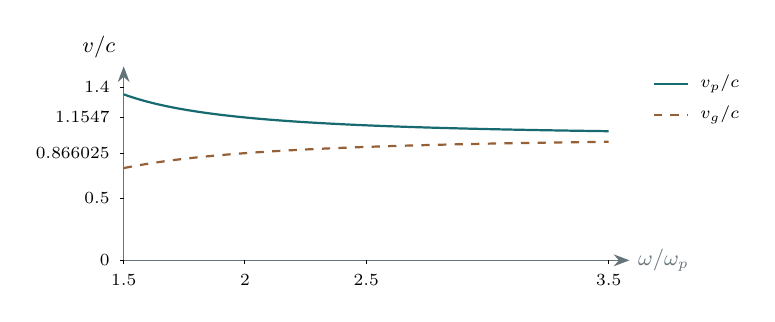
\begin{tikzpicture}[scale=.88,transform shape]
\draw[axis] (0,0.0)--(7.3,0.0) node[right] {$\omega/\omega_p$};
\draw[axis] (0,0)--(0,2.8);
\node[above left] at (0,2.8) {$v/c$};
\draw[thin] (0.000000,0.0)--(0.000000,-0.06);\node[below,font=\scriptsize] at (0.000000,-0.08) {$ 1.5 $};
\draw[thin] (1.750000,0.0)--(1.750000,-0.06);\node[below,font=\scriptsize] at (1.750000,-0.08) {$ 2 $};
\draw[thin] (3.500000,0.0)--(3.500000,-0.06);\node[below,font=\scriptsize] at (3.500000,-0.08) {$ 2.5 $};
\draw[thin] (7.000000,0.0)--(7.000000,-0.06);\node[below,font=\scriptsize] at (7.000000,-0.08) {$ 3.5 $};
\draw[thin] (0,0.000000)--(-.06,0.000000);\node[left,font=\scriptsize] at (-.08,0.000000) {$ 0 $};
\draw[thin] (0,0.892857)--(-.06,0.892857);\node[left,font=\scriptsize] at (-.08,0.892857) {$ 0.5 $};
\draw[thin] (0,1.546473)--(-.06,1.546473);\node[left,font=\scriptsize] at (-.08,1.546473) {$ 0.866025 $};
\draw[thin] (0,2.061966)--(-.06,2.061966);\node[left,font=\scriptsize] at (-.08,2.061966) {$ 1.1547 $};
\draw[thin] (0,2.500000)--(-.06,2.500000);\node[left,font=\scriptsize] at (-.08,2.500000) {$ 1.4 $};
\draw[thick,color=accent] plot coordinates {(0.0000000,2.3957871) (0.0291667,2.3852966) (0.0583333,2.3751117) (0.0875000,2.3652196) (0.1166667,2.3556080) (0.1458333,2.3462652) (0.1750000,2.3371804) (0.2041667,2.3283432) (0.2333333,2.3197437) (0.2625000,2.3113728) (0.2916667,2.3032215) (0.3208333,2.2952816) (0.3500000,2.2875451) (0.3791667,2.2800044) (0.4083333,2.2726524) (0.4375000,2.2654823) (0.4666667,2.2584876) (0.4958333,2.2516620) (0.5250000,2.2449998) (0.5541667,2.2384952) (0.5833333,2.2321429) (0.6125000,2.2259377) (0.6416667,2.2198748) (0.6708333,2.2139495) (0.7000000,2.2081572) (0.7291667,2.2024938) (0.7583333,2.1969550) (0.7875000,2.1915370) (0.8166667,2.1862360) (0.8458333,2.1810484) (0.8750000,2.1759707) (0.9041667,2.1709996) (0.9333333,2.1661318) (0.9625000,2.1613644) (0.9916667,2.1566943) (1.0208333,2.1521187) (1.0500000,2.1476350) (1.0791667,2.1432404) (1.1083333,2.1389325) (1.1375000,2.1347088) (1.1666667,2.1305670) (1.1958333,2.1265048) (1.2250000,2.1225201) (1.2541667,2.1186107) (1.2833333,2.1147747) (1.3125000,2.1110100) (1.3416667,2.1073149) (1.3708333,2.1036874) (1.4000000,2.1001258) (1.4291667,2.0966285) (1.4583333,2.0931938) (1.4875000,2.0898201) (1.5166667,2.0865059) (1.5458333,2.0832497) (1.5750000,2.0800500) (1.6041667,2.0769055) (1.6333333,2.0738149) (1.6625000,2.0707767) (1.6916667,2.0677899) (1.7208333,2.0648531) (1.7500000,2.0619652) (1.7791667,2.0591251) (1.8083333,2.0563315) (1.8375000,2.0535836) (1.8666667,2.0508801) (1.8958333,2.0482201) (1.9250000,2.0456026) (1.9541667,2.0430267) (1.9833333,2.0404914) (2.0125000,2.0379958) (2.0416667,2.0355391) (2.0708333,2.0331204) (2.1000000,2.0307389) (2.1291667,2.0283937) (2.1583333,2.0260842) (2.1875000,2.0238095) (2.2166667,2.0215690) (2.2458333,2.0193618) (2.2750000,2.0171873) (2.3041667,2.0150449) (2.3333333,2.0129339) (2.3625000,2.0108535) (2.3916667,2.0088033) (2.4208333,2.0067825) (2.4500000,2.0047907) (2.4791667,2.0028272) (2.5083333,2.0008915) (2.5375000,1.9989829) (2.5666667,1.9971011) (2.5958333,1.9952454) (2.6250000,1.9934154) (2.6541667,1.9916105) (2.6833333,1.9898303) (2.7125000,1.9880744) (2.7416667,1.9863422) (2.7708333,1.9846333) (2.8000000,1.9829473) (2.8291667,1.9812837) (2.8583333,1.9796421) (2.8875000,1.9780222) (2.9166667,1.9764235) (2.9458333,1.9748457) (2.9750000,1.9732883) (3.0041667,1.9717511) (3.0333333,1.9702335) (3.0625000,1.9687354) (3.0916667,1.9672563) (3.1208333,1.9657959) (3.1500000,1.9643539) (3.1791667,1.9629300) (3.2083333,1.9615238) (3.2375000,1.9601351) (3.2666667,1.9587635) (3.2958333,1.9574087) (3.3250000,1.9560705) (3.3541667,1.9547486) (3.3833333,1.9534427) (3.4125000,1.9521526) (3.4416667,1.9508779) (3.4708333,1.9496185) (3.5000000,1.9483740) (3.5291667,1.9471443) (3.5583333,1.9459290) (3.5875000,1.9447280) (3.6166667,1.9435410) (3.6458333,1.9423679) (3.6750000,1.9412082) (3.7041667,1.9400620) (3.7333333,1.9389289) (3.7625000,1.9378087) (3.7916667,1.9367013) (3.8208333,1.9356064) (3.8500000,1.9345238) (3.8791667,1.9334534) (3.9083333,1.9323949) (3.9375000,1.9313483) (3.9666667,1.9303132) (3.9958333,1.9292895) (4.0250000,1.9282771) (4.0541667,1.9272758) (4.0833333,1.9262853) (4.1125000,1.9253056) (4.1416667,1.9243365) (4.1708333,1.9233779) (4.2000000,1.9224295) (4.2291667,1.9214912) (4.2583333,1.9205629) (4.2875000,1.9196444) (4.3166667,1.9187356) (4.3458333,1.9178364) (4.3750000,1.9169466) (4.4041667,1.9160660) (4.4333333,1.9151946) (4.4625000,1.9143322) (4.4916667,1.9134787) (4.5208333,1.9126339) (4.5500000,1.9117978) (4.5791667,1.9109702) (4.6083333,1.9101509) (4.6375000,1.9093400) (4.6666667,1.9085372) (4.6958333,1.9077425) (4.7250000,1.9069557) (4.7541667,1.9061767) (4.7833333,1.9054055) (4.8125000,1.9046419) (4.8416667,1.9038858) (4.8708333,1.9031371) (4.9000000,1.9023957) (4.9291667,1.9016616) (4.9583333,1.9009346) (4.9875000,1.9002146) (5.0166667,1.8995015) (5.0458333,1.8987953) (5.0750000,1.8980958) (5.1041667,1.8974030) (5.1333333,1.8967168) (5.1625000,1.8960371) (5.1916667,1.8953638) (5.2208333,1.8946968) (5.2500000,1.8940360) (5.2791667,1.8933814) (5.3083333,1.8927329) (5.3375000,1.8920905) (5.3666667,1.8914539) (5.3958333,1.8908232) (5.4250000,1.8901983) (5.4541667,1.8895791) (5.4833333,1.8889656) (5.5125000,1.8883576) (5.5416667,1.8877551) (5.5708333,1.8871581) (5.6000000,1.8865664) (5.6291667,1.8859800) (5.6583333,1.8853989) (5.6875000,1.8848229) (5.7166667,1.8842521) (5.7458333,1.8836862) (5.7750000,1.8831254) (5.8041667,1.8825695) (5.8333333,1.8820185) (5.8625000,1.8814723) (5.8916667,1.8809309) (5.9208333,1.8803941) (5.9500000,1.8798620) (5.9791667,1.8793345) (6.0083333,1.8788115) (6.0375000,1.8782929) (6.0666667,1.8777789) (6.0958333,1.8772691) (6.1250000,1.8767638) (6.1541667,1.8762627) (6.1833333,1.8757658) (6.2125000,1.8752731) (6.2416667,1.8747845) (6.2708333,1.8743000) (6.3000000,1.8738196) (6.3291667,1.8733431) (6.3583333,1.8728706) (6.3875000,1.8724020) (6.4166667,1.8719372) (6.4458333,1.8714763) (6.4750000,1.8710191) (6.5041667,1.8705657) (6.5333333,1.8701159) (6.5625000,1.8696698) (6.5916667,1.8692273) (6.6208333,1.8687884) (6.6500000,1.8683530) (6.6791667,1.8679211) (6.7083333,1.8674926) (6.7375000,1.8670676) (6.7666667,1.8666459) (6.7958333,1.8662276) (6.8250000,1.8658126) (6.8541667,1.8654009) (6.8833333,1.8649923) (6.9125000,1.8645870) (6.9416667,1.8641849) (6.9708333,1.8637859) (7.0000000,1.8633900)};
\draw[thick,color=accent] (7.65,2.55)--(8.15,2.55);\node[right,font=\scriptsize] at (8.2,2.55) {$v_p/c$};
\draw[thick,dashed,color=warm] plot coordinates {(0.0000000,1.3309928) (0.0291667,1.3368466) (0.0583333,1.3425792) (0.0875000,1.3481943) (0.1166667,1.3536953) (0.1458333,1.3590857) (0.1750000,1.3643686) (0.2041667,1.3695470) (0.2333333,1.3746241) (0.2625000,1.3796024) (0.2916667,1.3844849) (0.3208333,1.3892742) (0.3500000,1.3939728) (0.3791667,1.3985831) (0.4083333,1.4031074) (0.4375000,1.4075482) (0.4666667,1.4119075) (0.4958333,1.4161874) (0.5250000,1.4203901) (0.5541667,1.4245175) (0.5833333,1.4285714) (0.6125000,1.4325538) (0.6416667,1.4364664) (0.6708333,1.4403109) (0.7000000,1.4440890) (0.7291667,1.4478023) (0.7583333,1.4514523) (0.7875000,1.4550407) (0.8166667,1.4585687) (0.8458333,1.4620379) (0.8750000,1.4654497) (0.9041667,1.4688052) (0.9333333,1.4721059) (0.9625000,1.4753531) (0.9916667,1.4785478) (1.0208333,1.4816913) (1.0500000,1.4847847) (1.0791667,1.4878291) (1.1083333,1.4908257) (1.1375000,1.4937754) (1.1666667,1.4966793) (1.1958333,1.4995383) (1.2250000,1.5023535) (1.2541667,1.5051257) (1.2833333,1.5078559) (1.3125000,1.5105449) (1.3416667,1.5131937) (1.3708333,1.5158029) (1.4000000,1.5183735) (1.4291667,1.5209063) (1.4583333,1.5234019) (1.4875000,1.5258612) (1.5166667,1.5282849) (1.5458333,1.5306737) (1.5750000,1.5330283) (1.6041667,1.5353493) (1.6333333,1.5376375) (1.6625000,1.5398934) (1.6916667,1.5421177) (1.7208333,1.5443110) (1.7500000,1.5464739) (1.7791667,1.5486070) (1.8083333,1.5507108) (1.8375000,1.5527859) (1.8666667,1.5548328) (1.8958333,1.5568520) (1.9250000,1.5588441) (1.9541667,1.5608095) (1.9833333,1.5627488) (2.0125000,1.5646625) (2.0416667,1.5665509) (2.0708333,1.5684145) (2.1000000,1.5702539) (2.1291667,1.5720693) (2.1583333,1.5738613) (2.1875000,1.5756303) (2.2166667,1.5773766) (2.2458333,1.5791006) (2.2750000,1.5808028) (2.3041667,1.5824836) (2.3333333,1.5841432) (2.3625000,1.5857821) (2.3916667,1.5874006) (2.4208333,1.5889990) (2.4500000,1.5905778) (2.4791667,1.5921371) (2.5083333,1.5936774) (2.5375000,1.5951990) (2.5666667,1.5967021) (2.5958333,1.5981871) (2.6250000,1.5996543) (2.6541667,1.6011040) (2.6833333,1.6025364) (2.7125000,1.6039518) (2.7416667,1.6053506) (2.7708333,1.6067329) (2.8000000,1.6080990) (2.8291667,1.6094492) (2.8583333,1.6107838) (2.8875000,1.6121030) (2.9166667,1.6134070) (2.9458333,1.6146960) (2.9750000,1.6159704) (3.0041667,1.6172303) (3.0333333,1.6184759) (3.0625000,1.6197075) (3.0916667,1.6209253) (3.1208333,1.6221295) (3.1500000,1.6233203) (3.1791667,1.6244978) (3.2083333,1.6256624) (3.2375000,1.6268142) (3.2666667,1.6279533) (3.2958333,1.6290801) (3.3250000,1.6301946) (3.3541667,1.6312970) (3.3833333,1.6323875) (3.4125000,1.6334663) (3.4416667,1.6345336) (3.4708333,1.6355895) (3.5000000,1.6366342) (3.5291667,1.6376678) (3.5583333,1.6386906) (3.5875000,1.6397026) (3.6166667,1.6407040) (3.6458333,1.6416950) (3.6750000,1.6426756) (3.7041667,1.6436462) (3.7333333,1.6446067) (3.7625000,1.6455574) (3.7916667,1.6464984) (3.8208333,1.6474297) (3.8500000,1.6483516) (3.8791667,1.6492642) (3.9083333,1.6501676) (3.9375000,1.6510619) (3.9666667,1.6519472) (3.9958333,1.6528237) (4.0250000,1.6536915) (4.0541667,1.6545507) (4.0833333,1.6554014) (4.1125000,1.6562438) (4.1416667,1.6570779) (4.1708333,1.6579038) (4.2000000,1.6587217) (4.2291667,1.6595317) (4.2583333,1.6603338) (4.2875000,1.6611282) (4.3166667,1.6619150) (4.3458333,1.6626942) (4.3750000,1.6634660) (4.4041667,1.6642305) (4.4333333,1.6649877) (4.4625000,1.6657378) (4.4916667,1.6664808) (4.5208333,1.6672169) (4.5500000,1.6679460) (4.5791667,1.6686684) (4.6083333,1.6693840) (4.6375000,1.6700931) (4.6666667,1.6707956) (4.6958333,1.6714916) (4.7250000,1.6721812) (4.7541667,1.6728646) (4.7833333,1.6735417) (4.8125000,1.6742126) (4.8416667,1.6748775) (4.8708333,1.6755364) (4.9000000,1.6761894) (4.9291667,1.6768365) (4.9583333,1.6774778) (4.9875000,1.6781134) (5.0166667,1.6787433) (5.0458333,1.6793677) (5.0750000,1.6799866) (5.1041667,1.6806000) (5.1333333,1.6812080) (5.1625000,1.6818107) (5.1916667,1.6824082) (5.2208333,1.6830004) (5.2500000,1.6835876) (5.2791667,1.6841696) (5.3083333,1.6847467) (5.3375000,1.6853187) (5.3666667,1.6858859) (5.3958333,1.6864483) (5.4250000,1.6870058) (5.4541667,1.6875586) (5.4833333,1.6881067) (5.5125000,1.6886503) (5.5416667,1.6891892) (5.5708333,1.6897236) (5.6000000,1.6902535) (5.6291667,1.6907791) (5.6583333,1.6913002) (5.6875000,1.6918170) (5.7166667,1.6923296) (5.7458333,1.6928379) (5.7750000,1.6933421) (5.8041667,1.6938421) (5.8333333,1.6943380) (5.8625000,1.6948299) (5.8916667,1.6953178) (5.9208333,1.6958017) (5.9500000,1.6962817) (5.9791667,1.6967579) (6.0083333,1.6972302) (6.0375000,1.6976987) (6.0666667,1.6981635) (6.0958333,1.6986246) (6.1250000,1.6990820) (6.1541667,1.6995358) (6.1833333,1.6999860) (6.2125000,1.7004326) (6.2416667,1.7008758) (6.2708333,1.7013154) (6.3000000,1.7017516) (6.3291667,1.7021845) (6.3583333,1.7026139) (6.3875000,1.7030400) (6.4166667,1.7034629) (6.4458333,1.7038824) (6.4750000,1.7042988) (6.5041667,1.7047119) (6.5333333,1.7051219) (6.5625000,1.7055287) (6.5916667,1.7059324) (6.6208333,1.7063331) (6.6500000,1.7067308) (6.6791667,1.7071254) (6.7083333,1.7075171) (6.7375000,1.7079058) (6.7666667,1.7082916) (6.7958333,1.7086745) (6.8250000,1.7090546) (6.8541667,1.7094318) (6.8833333,1.7098062) (6.9125000,1.7101779) (6.9416667,1.7105468) (6.9708333,1.7109130) (7.0000000,1.7112765)};
\draw[thick,dashed,color=warm] (7.65,2.0999999999999996)--(8.15,2.0999999999999996);\node[right,font=\scriptsize] at (8.2,2.0999999999999996) {$v_g/c$};
\end{tikzpicture}
\figcaption{变图光5.4V3\quad 两倍特征频率的相速1.154701c与群速0.866025c}
\end{minipage}\end{center}
\item \textbf{保留非零束缚频率。}设$n^2=1+\omega_p^2/(\omega_r^2-\omega^2)$，在无损实传播区求$v_pv_g$，取$\omega_r=.5\omega_p,\omega=2\omega_p$给数值。

由$n_g=n+\omega\dd n/\dd\omega$，有$n n_g=n^2+\omega^2\omega_p^2/(\omega_r^2-\omega^2)^2=1+\omega_p^2\omega_r^2/(\omega_r^2-\omega^2)^2$。因此
\[
 \frac{v_pv_g}{c^2}=\left[1+\frac{\omega_p^2\omega_r^2}{(\omega_r^2-\omega^2)^2}\right]^{-1}.
\]
变图光5.4V4取$\omega_r=.5\omega_p$，在$2\omega_p$处乘积为$.98253275c^2$；$\omega_r\to0$时额外项趋零，恢复自由高频平方型色散的乘积。
\begin{center}\begin{minipage}{.98\linewidth}\centering
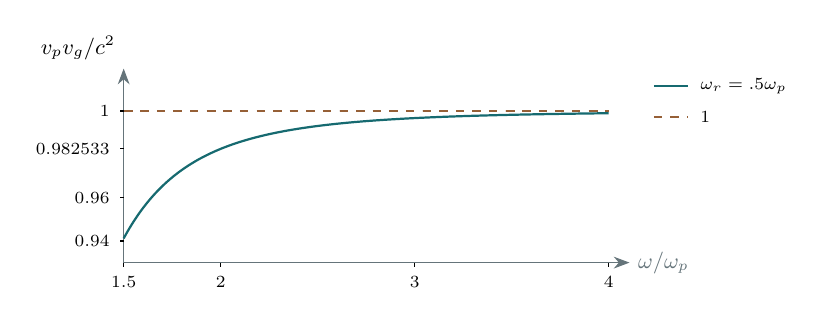
\begin{tikzpicture}[scale=.88,transform shape]
\draw[axis] (0,0)--(7.3,0) node[right] {$\omega/\omega_p$};
\draw[axis] (0,0)--(0,2.8);
\node[above left] at (0,2.8) {$v_pv_g/c^2$};
\draw[thin] (0.000000,0)--(0.000000,-0.06);\node[below,font=\scriptsize] at (0.000000,-0.08) {$ 1.5 $};
\draw[thin] (1.400000,0)--(1.400000,-0.06);\node[below,font=\scriptsize] at (1.400000,-0.08) {$ 2 $};
\draw[thin] (4.200000,0)--(4.200000,-0.06);\node[below,font=\scriptsize] at (4.200000,-0.08) {$ 3 $};
\draw[thin] (7.000000,0)--(7.000000,-0.06);\node[below,font=\scriptsize] at (7.000000,-0.08) {$ 4 $};
\draw[thin] (0,0.312500)--(-.06,0.312500);\node[left,font=\scriptsize] at (-.08,0.312500) {$ 0.94 $};
\draw[thin] (0,0.937500)--(-.06,0.937500);\node[left,font=\scriptsize] at (-.08,0.937500) {$ 0.96 $};
\draw[thin] (0,1.641656)--(-.06,1.641656);\node[left,font=\scriptsize] at (-.08,1.641656) {$ 0.982533 $};
\draw[thin] (0,2.187500)--(-.06,2.187500);\node[left,font=\scriptsize] at (-.08,2.187500) {$ 1 $};
\draw[thick,color=accent] plot coordinates {(0.0000000,0.3492647) (0.0291667,0.4023641) (0.0583333,0.4535840) (0.0875000,0.5030017) (0.1166667,0.5506910) (0.1458333,0.5967223) (0.1750000,0.6411627) (0.2041667,0.6840765) (0.2333333,0.7255249) (0.2625000,0.7655664) (0.2916667,0.8042568) (0.3208333,0.8416497) (0.3500000,0.8777959) (0.3791667,0.9127443) (0.4083333,0.9465415) (0.4375000,0.9792320) (0.4666667,1.0108585) (0.4958333,1.0414617) (0.5250000,1.0710806) (0.5541667,1.0997524) (0.5833333,1.1275130) (0.6125000,1.1543964) (0.6416667,1.1804354) (0.6708333,1.2056613) (0.7000000,1.2301041) (0.7291667,1.2537926) (0.7583333,1.2767542) (0.7875000,1.2990153) (0.8166667,1.3206014) (0.8458333,1.3415365) (0.8750000,1.3618440) (0.9041667,1.3815462) (0.9333333,1.4006644) (0.9625000,1.4192193) (0.9916667,1.4372304) (1.0208333,1.4547167) (1.0500000,1.4716964) (1.0791667,1.4881869) (1.1083333,1.5042049) (1.1375000,1.5197666) (1.1666667,1.5348873) (1.1958333,1.5495820) (1.2250000,1.5638650) (1.2541667,1.5777498) (1.2833333,1.5912499) (1.3125000,1.6043778) (1.3416667,1.6171458) (1.3708333,1.6295655) (1.4000000,1.6416485) (1.4291667,1.6534054) (1.4583333,1.6648469) (1.4875000,1.6759829) (1.5166667,1.6868233) (1.5458333,1.6973773) (1.5750000,1.7076540) (1.6041667,1.7176621) (1.6333333,1.7274100) (1.6625000,1.7369057) (1.6916667,1.7461570) (1.7208333,1.7551714) (1.7500000,1.7639563) (1.7791667,1.7725184) (1.8083333,1.7808647) (1.8375000,1.7890015) (1.8666667,1.7969353) (1.8958333,1.8046719) (1.9250000,1.8122173) (1.9541667,1.8195772) (1.9833333,1.8267569) (2.0125000,1.8337618) (2.0416667,1.8405969) (2.0708333,1.8472672) (2.1000000,1.8537773) (2.1291667,1.8601320) (2.1583333,1.8663356) (2.1875000,1.8723925) (2.2166667,1.8783067) (2.2458333,1.8840823) (2.2750000,1.8897233) (2.3041667,1.8952332) (2.3333333,1.9006159) (2.3625000,1.9058748) (2.3916667,1.9110133) (2.4208333,1.9160347) (2.4500000,1.9209422) (2.4791667,1.9257389) (2.5083333,1.9304278) (2.5375000,1.9350117) (2.5666667,1.9394936) (2.5958333,1.9438761) (2.6250000,1.9481619) (2.6541667,1.9523535) (2.6833333,1.9564533) (2.7125000,1.9604639) (2.7416667,1.9643875) (2.7708333,1.9682264) (2.8000000,1.9719828) (2.8291667,1.9756587) (2.8583333,1.9792563) (2.8875000,1.9827776) (2.9166667,1.9862245) (2.9458333,1.9895989) (2.9750000,1.9929026) (3.0041667,1.9961374) (3.0333333,1.9993049) (3.0625000,2.0024070) (3.0916667,2.0054452) (3.1208333,2.0084210) (3.1500000,2.0113361) (3.1791667,2.0141918) (3.2083333,2.0169897) (3.2375000,2.0197312) (3.2666667,2.0224176) (3.2958333,2.0250502) (3.3250000,2.0276303) (3.3541667,2.0301593) (3.3833333,2.0326382) (3.4125000,2.0350683) (3.4416667,2.0374508) (3.4708333,2.0397867) (3.5000000,2.0420772) (3.5291667,2.0443233) (3.5583333,2.0465260) (3.5875000,2.0486863) (3.6166667,2.0508053) (3.6458333,2.0528839) (3.6750000,2.0549229) (3.7041667,2.0569234) (3.7333333,2.0588861) (3.7625000,2.0608120) (3.7916667,2.0627018) (3.8208333,2.0645563) (3.8500000,2.0663764) (3.8791667,2.0681629) (3.9083333,2.0699164) (3.9375000,2.0716377) (3.9666667,2.0733275) (3.9958333,2.0749864) (4.0250000,2.0766153) (4.0541667,2.0782147) (4.0833333,2.0797852) (4.1125000,2.0813276) (4.1416667,2.0828423) (4.1708333,2.0843300) (4.2000000,2.0857913) (4.2291667,2.0872267) (4.2583333,2.0886368) (4.2875000,2.0900221) (4.3166667,2.0913831) (4.3458333,2.0927204) (4.3750000,2.0940344) (4.4041667,2.0953257) (4.4333333,2.0965946) (4.4625000,2.0978417) (4.4916667,2.0990675) (4.5208333,2.1002723) (4.5500000,2.1014565) (4.5791667,2.1026207) (4.6083333,2.1037652) (4.6375000,2.1048903) (4.6666667,2.1059966) (4.6958333,2.1070844) (4.7250000,2.1081540) (4.7541667,2.1092059) (4.7833333,2.1102403) (4.8125000,2.1112576) (4.8416667,2.1122582) (4.8708333,2.1132423) (4.9000000,2.1142104) (4.9291667,2.1151627) (4.9583333,2.1160995) (4.9875000,2.1170212) (5.0166667,2.1179280) (5.0458333,2.1188202) (5.0750000,2.1196981) (5.1041667,2.1205620) (5.1333333,2.1214121) (5.1625000,2.1222487) (5.1916667,2.1230721) (5.2208333,2.1238825) (5.2500000,2.1246801) (5.2791667,2.1254653) (5.3083333,2.1262382) (5.3375000,2.1269990) (5.3666667,2.1277481) (5.3958333,2.1284855) (5.4250000,2.1292116) (5.4541667,2.1299265) (5.4833333,2.1306304) (5.5125000,2.1313236) (5.5416667,2.1320062) (5.5708333,2.1326785) (5.6000000,2.1333406) (5.6291667,2.1339926) (5.6583333,2.1346349) (5.6875000,2.1352675) (5.7166667,2.1358907) (5.7458333,2.1365046) (5.7750000,2.1371093) (5.8041667,2.1377051) (5.8333333,2.1382921) (5.8625000,2.1388704) (5.8916667,2.1394402) (5.9208333,2.1400017) (5.9500000,2.1405550) (5.9791667,2.1411002) (6.0083333,2.1416376) (6.0375000,2.1421671) (6.0666667,2.1426890) (6.0958333,2.1432034) (6.1250000,2.1437104) (6.1541667,2.1442101) (6.1833333,2.1447028) (6.2125000,2.1451884) (6.2416667,2.1456671) (6.2708333,2.1461391) (6.3000000,2.1466044) (6.3291667,2.1470631) (6.3583333,2.1475155) (6.3875000,2.1479615) (6.4166667,2.1484013) (6.4458333,2.1488349) (6.4750000,2.1492626) (6.5041667,2.1496844) (6.5333333,2.1501003) (6.5625000,2.1505105) (6.5916667,2.1509151) (6.6208333,2.1513142) (6.6500000,2.1517078) (6.6791667,2.1520960) (6.7083333,2.1524791) (6.7375000,2.1528569) (6.7666667,2.1532296) (6.7958333,2.1535973) (6.8250000,2.1539601) (6.8541667,2.1543181) (6.8833333,2.1546712) (6.9125000,2.1550197) (6.9416667,2.1553635) (6.9708333,2.1557028) (7.0000000,2.1560376)};
\draw[thick,color=accent] (7.65,2.55)--(8.15,2.55);\node[right,font=\scriptsize] at (8.2,2.55) {$\omega_r=.5\omega_p$};
\draw[thick,dashed,color=warm] plot coordinates {(0.0000000,2.1875000) (0.0291667,2.1875000) (0.0583333,2.1875000) (0.0875000,2.1875000) (0.1166667,2.1875000) (0.1458333,2.1875000) (0.1750000,2.1875000) (0.2041667,2.1875000) (0.2333333,2.1875000) (0.2625000,2.1875000) (0.2916667,2.1875000) (0.3208333,2.1875000) (0.3500000,2.1875000) (0.3791667,2.1875000) (0.4083333,2.1875000) (0.4375000,2.1875000) (0.4666667,2.1875000) (0.4958333,2.1875000) (0.5250000,2.1875000) (0.5541667,2.1875000) (0.5833333,2.1875000) (0.6125000,2.1875000) (0.6416667,2.1875000) (0.6708333,2.1875000) (0.7000000,2.1875000) (0.7291667,2.1875000) (0.7583333,2.1875000) (0.7875000,2.1875000) (0.8166667,2.1875000) (0.8458333,2.1875000) (0.8750000,2.1875000) (0.9041667,2.1875000) (0.9333333,2.1875000) (0.9625000,2.1875000) (0.9916667,2.1875000) (1.0208333,2.1875000) (1.0500000,2.1875000) (1.0791667,2.1875000) (1.1083333,2.1875000) (1.1375000,2.1875000) (1.1666667,2.1875000) (1.1958333,2.1875000) (1.2250000,2.1875000) (1.2541667,2.1875000) (1.2833333,2.1875000) (1.3125000,2.1875000) (1.3416667,2.1875000) (1.3708333,2.1875000) (1.4000000,2.1875000) (1.4291667,2.1875000) (1.4583333,2.1875000) (1.4875000,2.1875000) (1.5166667,2.1875000) (1.5458333,2.1875000) (1.5750000,2.1875000) (1.6041667,2.1875000) (1.6333333,2.1875000) (1.6625000,2.1875000) (1.6916667,2.1875000) (1.7208333,2.1875000) (1.7500000,2.1875000) (1.7791667,2.1875000) (1.8083333,2.1875000) (1.8375000,2.1875000) (1.8666667,2.1875000) (1.8958333,2.1875000) (1.9250000,2.1875000) (1.9541667,2.1875000) (1.9833333,2.1875000) (2.0125000,2.1875000) (2.0416667,2.1875000) (2.0708333,2.1875000) (2.1000000,2.1875000) (2.1291667,2.1875000) (2.1583333,2.1875000) (2.1875000,2.1875000) (2.2166667,2.1875000) (2.2458333,2.1875000) (2.2750000,2.1875000) (2.3041667,2.1875000) (2.3333333,2.1875000) (2.3625000,2.1875000) (2.3916667,2.1875000) (2.4208333,2.1875000) (2.4500000,2.1875000) (2.4791667,2.1875000) (2.5083333,2.1875000) (2.5375000,2.1875000) (2.5666667,2.1875000) (2.5958333,2.1875000) (2.6250000,2.1875000) (2.6541667,2.1875000) (2.6833333,2.1875000) (2.7125000,2.1875000) (2.7416667,2.1875000) (2.7708333,2.1875000) (2.8000000,2.1875000) (2.8291667,2.1875000) (2.8583333,2.1875000) (2.8875000,2.1875000) (2.9166667,2.1875000) (2.9458333,2.1875000) (2.9750000,2.1875000) (3.0041667,2.1875000) (3.0333333,2.1875000) (3.0625000,2.1875000) (3.0916667,2.1875000) (3.1208333,2.1875000) (3.1500000,2.1875000) (3.1791667,2.1875000) (3.2083333,2.1875000) (3.2375000,2.1875000) (3.2666667,2.1875000) (3.2958333,2.1875000) (3.3250000,2.1875000) (3.3541667,2.1875000) (3.3833333,2.1875000) (3.4125000,2.1875000) (3.4416667,2.1875000) (3.4708333,2.1875000) (3.5000000,2.1875000) (3.5291667,2.1875000) (3.5583333,2.1875000) (3.5875000,2.1875000) (3.6166667,2.1875000) (3.6458333,2.1875000) (3.6750000,2.1875000) (3.7041667,2.1875000) (3.7333333,2.1875000) (3.7625000,2.1875000) (3.7916667,2.1875000) (3.8208333,2.1875000) (3.8500000,2.1875000) (3.8791667,2.1875000) (3.9083333,2.1875000) (3.9375000,2.1875000) (3.9666667,2.1875000) (3.9958333,2.1875000) (4.0250000,2.1875000) (4.0541667,2.1875000) (4.0833333,2.1875000) (4.1125000,2.1875000) (4.1416667,2.1875000) (4.1708333,2.1875000) (4.2000000,2.1875000) (4.2291667,2.1875000) (4.2583333,2.1875000) (4.2875000,2.1875000) (4.3166667,2.1875000) (4.3458333,2.1875000) (4.3750000,2.1875000) (4.4041667,2.1875000) (4.4333333,2.1875000) (4.4625000,2.1875000) (4.4916667,2.1875000) (4.5208333,2.1875000) (4.5500000,2.1875000) (4.5791667,2.1875000) (4.6083333,2.1875000) (4.6375000,2.1875000) (4.6666667,2.1875000) (4.6958333,2.1875000) (4.7250000,2.1875000) (4.7541667,2.1875000) (4.7833333,2.1875000) (4.8125000,2.1875000) (4.8416667,2.1875000) (4.8708333,2.1875000) (4.9000000,2.1875000) (4.9291667,2.1875000) (4.9583333,2.1875000) (4.9875000,2.1875000) (5.0166667,2.1875000) (5.0458333,2.1875000) (5.0750000,2.1875000) (5.1041667,2.1875000) (5.1333333,2.1875000) (5.1625000,2.1875000) (5.1916667,2.1875000) (5.2208333,2.1875000) (5.2500000,2.1875000) (5.2791667,2.1875000) (5.3083333,2.1875000) (5.3375000,2.1875000) (5.3666667,2.1875000) (5.3958333,2.1875000) (5.4250000,2.1875000) (5.4541667,2.1875000) (5.4833333,2.1875000) (5.5125000,2.1875000) (5.5416667,2.1875000) (5.5708333,2.1875000) (5.6000000,2.1875000) (5.6291667,2.1875000) (5.6583333,2.1875000) (5.6875000,2.1875000) (5.7166667,2.1875000) (5.7458333,2.1875000) (5.7750000,2.1875000) (5.8041667,2.1875000) (5.8333333,2.1875000) (5.8625000,2.1875000) (5.8916667,2.1875000) (5.9208333,2.1875000) (5.9500000,2.1875000) (5.9791667,2.1875000) (6.0083333,2.1875000) (6.0375000,2.1875000) (6.0666667,2.1875000) (6.0958333,2.1875000) (6.1250000,2.1875000) (6.1541667,2.1875000) (6.1833333,2.1875000) (6.2125000,2.1875000) (6.2416667,2.1875000) (6.2708333,2.1875000) (6.3000000,2.1875000) (6.3291667,2.1875000) (6.3583333,2.1875000) (6.3875000,2.1875000) (6.4166667,2.1875000) (6.4458333,2.1875000) (6.4750000,2.1875000) (6.5041667,2.1875000) (6.5333333,2.1875000) (6.5625000,2.1875000) (6.5916667,2.1875000) (6.6208333,2.1875000) (6.6500000,2.1875000) (6.6791667,2.1875000) (6.7083333,2.1875000) (6.7375000,2.1875000) (6.7666667,2.1875000) (6.7958333,2.1875000) (6.8250000,2.1875000) (6.8541667,2.1875000) (6.8833333,2.1875000) (6.9125000,2.1875000) (6.9416667,2.1875000) (6.9708333,2.1875000) (7.0000000,2.1875000)};
\draw[thick,dashed,color=warm] (7.65,2.0999999999999996)--(8.15,2.0999999999999996);\node[right,font=\scriptsize] at (8.2,2.0999999999999996) {$1$};
\end{tikzpicture}
\figcaption{变图光5.4V4\quad 非零束缚频率改变速度乘积}
\end{minipage}\end{center}
\item \textbf{X射线掠入射全外反射。}使用$.10\,\mathrm{nm}$处的$n$，真空侧入射，掠射角$\alpha$从表面量起。求全反射条件和临界掠射角。

切向波数连续给$k_z^2=(\omega^2/c^2)(n^2-\cos^2\alpha)$。当$\cos\alpha>n$时，法向根为正虚数，两个无损偏振都全反射。临界值为
\[
 \alpha_c=\arccos n=\arcsin(\sqrt K\lambda_0)
 \simeq\sqrt K\lambda_0=.255367^\circ.
\]
变图光5.4V5画$s,p$功率反射率，$\alpha<\alpha_c$时均为1，超过该角后出现向内传播功率。这里外部折射率1较大，临界条件用相对表面的小掠射角表示。
\begin{center}\begin{minipage}{.98\linewidth}\centering
\begin{tikzpicture}[scale=.88,transform shape]
\draw[axis] (0,0.0)--(7.3,0.0) node[right] {$\alpha/{}^\circ$};
\draw[axis] (0,0)--(0,2.8);
\node[above left] at (0,2.8) {$R_j$};
\draw[thin] (0.000000,0.0)--(0.000000,-0.06);\node[below,font=\scriptsize] at (0.000000,-0.08) {$ 0 $};
\draw[thin] (1.787569,0.0)--(1.787569,-0.06);\node[below,font=\scriptsize] at (1.787569,-0.08) {$ 0.255367 $};
\draw[thin] (3.500000,0.0)--(3.500000,-0.06);\node[below,font=\scriptsize] at (3.500000,-0.08) {$ 0.5 $};
\draw[thin] (7.000000,0.0)--(7.000000,-0.06);\node[below,font=\scriptsize] at (7.000000,-0.08) {$ 1 $};
\draw[thin] (0,0.000000)--(-.06,0.000000);\node[left,font=\scriptsize] at (-.08,0.000000) {$ 0 $};
\draw[thin] (0,1.213592)--(-.06,1.213592);\node[left,font=\scriptsize] at (-.08,1.213592) {$ 0.5 $};
\draw[thin] (0,2.427184)--(-.06,2.427184);\node[left,font=\scriptsize] at (-.08,2.427184) {$ 1 $};
\draw[thick,color=accent] plot coordinates {(0.0000000,2.4271845) (0.0291667,2.4271845) (0.0583333,2.4271845) (0.0875000,2.4271845) (0.1166667,2.4271845) (0.1458333,2.4271845) (0.1750000,2.4271845) (0.2041667,2.4271845) (0.2333333,2.4271845) (0.2625000,2.4271845) (0.2916667,2.4271845) (0.3208333,2.4271845) (0.3500000,2.4271845) (0.3791667,2.4271845) (0.4083333,2.4271845) (0.4375000,2.4271845) (0.4666667,2.4271845) (0.4958333,2.4271845) (0.5250000,2.4271845) (0.5541667,2.4271845) (0.5833333,2.4271845) (0.6125000,2.4271845) (0.6416667,2.4271845) (0.6708333,2.4271845) (0.7000000,2.4271845) (0.7291667,2.4271845) (0.7583333,2.4271845) (0.7875000,2.4271845) (0.8166667,2.4271845) (0.8458333,2.4271845) (0.8750000,2.4271845) (0.9041667,2.4271845) (0.9333333,2.4271845) (0.9625000,2.4271845) (0.9916667,2.4271845) (1.0208333,2.4271845) (1.0500000,2.4271845) (1.0791667,2.4271845) (1.1083333,2.4271845) (1.1375000,2.4271845) (1.1666667,2.4271845) (1.1958333,2.4271845) (1.2250000,2.4271845) (1.2541667,2.4271845) (1.2833333,2.4271845) (1.3125000,2.4271845) (1.3416667,2.4271845) (1.3708333,2.4271845) (1.4000000,2.4271845) (1.4291667,2.4271845) (1.4583333,2.4271845) (1.4875000,2.4271845) (1.5166667,2.4271845) (1.5458333,2.4271845) (1.5750000,2.4271845) (1.6041667,2.4271845) (1.6333333,2.4271845) (1.6625000,2.4271845) (1.6916667,2.4271845) (1.7208333,2.4271845) (1.7500000,2.4271845) (1.7791667,2.4271845) (1.8083333,1.3199965) (1.8375000,0.9450526) (1.8666667,0.7416581) (1.8958333,0.6074488) (1.9250000,0.5107406) (1.9541667,0.4373284) (1.9833333,0.3796110) (2.0125000,0.3330603) (2.0416667,0.2947745) (2.0708333,0.2627927) (2.1000000,0.2357348) (2.1291667,0.2125978) (2.1583333,0.1926334) (2.1875000,0.1752710) (2.2166667,0.1600678) (2.2458333,0.1466744) (2.2750000,0.1348116) (2.3041667,0.1242533) (2.3333333,0.1148147) (2.3625000,0.1063434) (2.3916667,0.0987123) (2.4208333,0.0918151) (2.4500000,0.0855617) (2.4791667,0.0798758) (2.5083333,0.0746920) (2.5375000,0.0699542) (2.5666667,0.0656138) (2.5958333,0.0616289) (2.6250000,0.0579628) (2.6541667,0.0545833) (2.6833333,0.0514624) (2.7125000,0.0485753) (2.7416667,0.0459001) (2.7708333,0.0434172) (2.8000000,0.0411095) (2.8291667,0.0389616) (2.8583333,0.0369596) (2.8875000,0.0350912) (2.9166667,0.0333454) (2.9458333,0.0317121) (2.9750000,0.0301824) (3.0041667,0.0287481) (3.0333333,0.0274019) (3.0625000,0.0261370) (3.0916667,0.0249475) (3.1208333,0.0238276) (3.1500000,0.0227725) (3.1791667,0.0217775) (3.2083333,0.0208384) (3.2375000,0.0199513) (3.2666667,0.0191126) (3.2958333,0.0183192) (3.3250000,0.0175680) (3.3541667,0.0168562) (3.3833333,0.0161814) (3.4125000,0.0155411) (3.4416667,0.0149332) (3.4708333,0.0143557) (3.5000000,0.0138068) (3.5291667,0.0132846) (3.5583333,0.0127876) (3.5875000,0.0123144) (3.6166667,0.0118634) (3.6458333,0.0114335) (3.6750000,0.0110235) (3.7041667,0.0106321) (3.7333333,0.0102585) (3.7625000,0.0099015) (3.7916667,0.0095604) (3.8208333,0.0092341) (3.8500000,0.0089221) (3.8791667,0.0086234) (3.9083333,0.0083374) (3.9375000,0.0080635) (3.9666667,0.0078009) (3.9958333,0.0075493) (4.0250000,0.0073079) (4.0541667,0.0070763) (4.0833333,0.0068540) (4.1125000,0.0066405) (4.1416667,0.0064355) (4.1708333,0.0062385) (4.2000000,0.0060491) (4.2291667,0.0058670) (4.2583333,0.0056918) (4.2875000,0.0055233) (4.3166667,0.0053610) (4.3458333,0.0052048) (4.3750000,0.0050544) (4.4041667,0.0049094) (4.4333333,0.0047697) (4.4625000,0.0046350) (4.4916667,0.0045051) (4.5208333,0.0043799) (4.5500000,0.0042590) (4.5791667,0.0041423) (4.6083333,0.0040297) (4.6375000,0.0039209) (4.6666667,0.0038158) (4.6958333,0.0037143) (4.7250000,0.0036162) (4.7541667,0.0035214) (4.7833333,0.0034296) (4.8125000,0.0033410) (4.8416667,0.0032551) (4.8708333,0.0031721) (4.9000000,0.0030918) (4.9291667,0.0030140) (4.9583333,0.0029386) (4.9875000,0.0028657) (5.0166667,0.0027950) (5.0458333,0.0027265) (5.0750000,0.0026602) (5.1041667,0.0025958) (5.1333333,0.0025335) (5.1625000,0.0024730) (5.1916667,0.0024143) (5.2208333,0.0023574) (5.2500000,0.0023021) (5.2791667,0.0022485) (5.3083333,0.0021965) (5.3375000,0.0021460) (5.3666667,0.0020969) (5.3958333,0.0020493) (5.4250000,0.0020030) (5.4541667,0.0019580) (5.4833333,0.0019143) (5.5125000,0.0018719) (5.5416667,0.0018306) (5.5708333,0.0017904) (5.6000000,0.0017514) (5.6291667,0.0017134) (5.6583333,0.0016765) (5.6875000,0.0016405) (5.7166667,0.0016056) (5.7458333,0.0015715) (5.7750000,0.0015384) (5.8041667,0.0015062) (5.8333333,0.0014748) (5.8625000,0.0014442) (5.8916667,0.0014144) (5.9208333,0.0013854) (5.9500000,0.0013571) (5.9791667,0.0013296) (6.0083333,0.0013028) (6.0375000,0.0012766) (6.0666667,0.0012511) (6.0958333,0.0012262) (6.1250000,0.0012020) (6.1541667,0.0011784) (6.1833333,0.0011553) (6.2125000,0.0011328) (6.2416667,0.0011109) (6.2708333,0.0010895) (6.3000000,0.0010686) (6.3291667,0.0010482) (6.3583333,0.0010283) (6.3875000,0.0010089) (6.4166667,0.0009899) (6.4458333,0.0009714) (6.4750000,0.0009533) (6.5041667,0.0009357) (6.5333333,0.0009184) (6.5625000,0.0009015) (6.5916667,0.0008851) (6.6208333,0.0008690) (6.6500000,0.0008533) (6.6791667,0.0008379) (6.7083333,0.0008229) (6.7375000,0.0008082) (6.7666667,0.0007939) (6.7958333,0.0007798) (6.8250000,0.0007661) (6.8541667,0.0007527) (6.8833333,0.0007396) (6.9125000,0.0007267) (6.9416667,0.0007142) (6.9708333,0.0007019) (7.0000000,0.0006899)};
\draw[thick,color=accent] (7.65,2.55)--(8.15,2.55);\node[right,font=\scriptsize] at (8.2,2.55) {$R_s$};
\draw[thick,dashed,color=warm] plot coordinates {(0.0000000,2.4271845) (0.0291667,2.4271845) (0.0583333,2.4271845) (0.0875000,2.4271845) (0.1166667,2.4271845) (0.1458333,2.4271845) (0.1750000,2.4271845) (0.2041667,2.4271845) (0.2333333,2.4271845) (0.2625000,2.4271845) (0.2916667,2.4271845) (0.3208333,2.4271845) (0.3500000,2.4271845) (0.3791667,2.4271845) (0.4083333,2.4271845) (0.4375000,2.4271845) (0.4666667,2.4271845) (0.4958333,2.4271845) (0.5250000,2.4271845) (0.5541667,2.4271845) (0.5833333,2.4271845) (0.6125000,2.4271845) (0.6416667,2.4271845) (0.6708333,2.4271845) (0.7000000,2.4271845) (0.7291667,2.4271845) (0.7583333,2.4271845) (0.7875000,2.4271845) (0.8166667,2.4271845) (0.8458333,2.4271845) (0.8750000,2.4271845) (0.9041667,2.4271845) (0.9333333,2.4271845) (0.9625000,2.4271845) (0.9916667,2.4271845) (1.0208333,2.4271845) (1.0500000,2.4271845) (1.0791667,2.4271845) (1.1083333,2.4271845) (1.1375000,2.4271845) (1.1666667,2.4271845) (1.1958333,2.4271845) (1.2250000,2.4271845) (1.2541667,2.4271845) (1.2833333,2.4271845) (1.3125000,2.4271845) (1.3416667,2.4271845) (1.3708333,2.4271845) (1.4000000,2.4271845) (1.4291667,2.4271845) (1.4583333,2.4271845) (1.4875000,2.4271845) (1.5166667,2.4271845) (1.5458333,2.4271845) (1.5750000,2.4271845) (1.6041667,2.4271845) (1.6333333,2.4271845) (1.6625000,2.4271845) (1.6916667,2.4271845) (1.7208333,2.4271845) (1.7500000,2.4271845) (1.7791667,2.4271845) (1.8083333,1.3199802) (1.8375000,0.9450342) (1.8666667,0.7416396) (1.8958333,0.6074307) (1.9250000,0.5107231) (1.9541667,0.4373116) (1.9833333,0.3795949) (2.0125000,0.3330449) (2.0416667,0.2947597) (2.0708333,0.2627786) (2.1000000,0.2357213) (2.1291667,0.2125848) (2.1583333,0.1926209) (2.1875000,0.1752590) (2.2166667,0.1600563) (2.2458333,0.1466633) (2.2750000,0.1348009) (2.3041667,0.1242429) (2.3333333,0.1148047) (2.3625000,0.1063337) (2.3916667,0.0987030) (2.4208333,0.0918060) (2.4500000,0.0855530) (2.4791667,0.0798673) (2.5083333,0.0746838) (2.5375000,0.0699462) (2.5666667,0.0656061) (2.5958333,0.0616214) (2.6250000,0.0579555) (2.6541667,0.0545763) (2.6833333,0.0514556) (2.7125000,0.0485687) (2.7416667,0.0458936) (2.7708333,0.0434109) (2.8000000,0.0411034) (2.8291667,0.0389556) (2.8583333,0.0369537) (2.8875000,0.0350855) (2.9166667,0.0333398) (2.9458333,0.0317067) (2.9750000,0.0301771) (3.0041667,0.0287429) (3.0333333,0.0273968) (3.0625000,0.0261321) (3.0916667,0.0249426) (3.1208333,0.0238229) (3.1500000,0.0227679) (3.1791667,0.0217730) (3.2083333,0.0208340) (3.2375000,0.0199469) (3.2666667,0.0191084) (3.2958333,0.0183151) (3.3250000,0.0175639) (3.3541667,0.0168523) (3.3833333,0.0161775) (3.4125000,0.0155373) (3.4416667,0.0149295) (3.4708333,0.0143521) (3.5000000,0.0138032) (3.5291667,0.0132810) (3.5583333,0.0127841) (3.5875000,0.0123109) (3.6166667,0.0118601) (3.6458333,0.0114302) (3.6750000,0.0110202) (3.7041667,0.0106289) (3.7333333,0.0102553) (3.7625000,0.0098985) (3.7916667,0.0095573) (3.8208333,0.0092312) (3.8500000,0.0089192) (3.8791667,0.0086205) (3.9083333,0.0083346) (3.9375000,0.0080607) (3.9666667,0.0077982) (3.9958333,0.0075466) (4.0250000,0.0073052) (4.0541667,0.0070737) (4.0833333,0.0068514) (4.1125000,0.0066380) (4.1416667,0.0064330) (4.1708333,0.0062360) (4.2000000,0.0060467) (4.2291667,0.0058646) (4.2583333,0.0056895) (4.2875000,0.0055210) (4.3166667,0.0053588) (4.3458333,0.0052026) (4.3750000,0.0050522) (4.4041667,0.0049073) (4.4333333,0.0047676) (4.4625000,0.0046329) (4.4916667,0.0045031) (4.5208333,0.0043778) (4.5500000,0.0042570) (4.5791667,0.0041403) (4.6083333,0.0040277) (4.6375000,0.0039190) (4.6666667,0.0038139) (4.6958333,0.0037124) (4.7250000,0.0036143) (4.7541667,0.0035195) (4.7833333,0.0034278) (4.8125000,0.0033392) (4.8416667,0.0032534) (4.8708333,0.0031704) (4.9000000,0.0030900) (4.9291667,0.0030123) (4.9583333,0.0029370) (4.9875000,0.0028640) (5.0166667,0.0027934) (5.0458333,0.0027249) (5.0750000,0.0026586) (5.1041667,0.0025943) (5.1333333,0.0025319) (5.1625000,0.0024714) (5.1916667,0.0024128) (5.2208333,0.0023559) (5.2500000,0.0023007) (5.2791667,0.0022471) (5.3083333,0.0021951) (5.3375000,0.0021446) (5.3666667,0.0020955) (5.3958333,0.0020479) (5.4250000,0.0020016) (5.4541667,0.0019567) (5.4833333,0.0019130) (5.5125000,0.0018705) (5.5416667,0.0018292) (5.5708333,0.0017891) (5.6000000,0.0017501) (5.6291667,0.0017121) (5.6583333,0.0016752) (5.6875000,0.0016393) (5.7166667,0.0016043) (5.7458333,0.0015703) (5.7750000,0.0015372) (5.8041667,0.0015050) (5.8333333,0.0014736) (5.8625000,0.0014430) (5.8916667,0.0014132) (5.9208333,0.0013842) (5.9500000,0.0013560) (5.9791667,0.0013285) (6.0083333,0.0013016) (6.0375000,0.0012755) (6.0666667,0.0012500) (6.0958333,0.0012252) (6.1250000,0.0012009) (6.1541667,0.0011773) (6.1833333,0.0011543) (6.2125000,0.0011318) (6.2416667,0.0011099) (6.2708333,0.0010885) (6.3000000,0.0010676) (6.3291667,0.0010472) (6.3583333,0.0010273) (6.3875000,0.0010079) (6.4166667,0.0009889) (6.4458333,0.0009704) (6.4750000,0.0009524) (6.5041667,0.0009347) (6.5333333,0.0009175) (6.5625000,0.0009006) (6.5916667,0.0008842) (6.6208333,0.0008681) (6.6500000,0.0008524) (6.6791667,0.0008370) (6.7083333,0.0008220) (6.7375000,0.0008073) (6.7666667,0.0007930) (6.7958333,0.0007790) (6.8250000,0.0007653) (6.8541667,0.0007518) (6.8833333,0.0007387) (6.9125000,0.0007259) (6.9416667,0.0007133) (6.9708333,0.0007011) (7.0000000,0.0006891)};
\draw[thick,dashed,color=warm] (7.65,2.0999999999999996)--(8.15,2.0999999999999996);\node[right,font=\scriptsize] at (8.2,2.0999999999999996) {$R_p$};
\end{tikzpicture}
\figcaption{变图光5.4V5\quad 小于0.255367度的掠射角产生无损全外反射}
\end{minipage}\end{center}
\item \textbf{一毫米样品的两种传播时间。}仍在$.10\,\mathrm{nm}$工作，求群时间相对真空及相对相位时间的差。

$t_g=L/(cn)$、$t_0=L/c$、$t_p=Ln/c$，因此
\[
 t_g-t_0=\frac Lc(1/n-1)=33.1082\,\mathrm{as},\qquad
 t_g-t_p=\frac Lc(1/n-n)=66.2162\,\mathrm{as}.
\]
变图光5.4V6随长度画这两个差值。近$n=1$时，第一项约为$L(1-n)/c$，第二项约为其两倍；相位面和包络在同一传播色散中具有不同计时关系。
\begin{center}\begin{minipage}{.98\linewidth}\centering
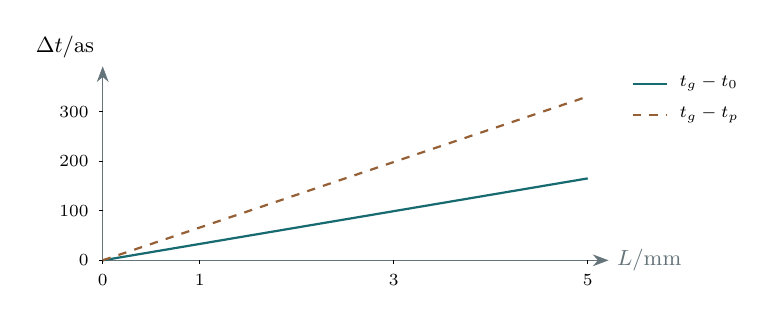
\begin{tikzpicture}[scale=.88,transform shape]
\draw[axis] (0,0.0)--(7.3,0.0) node[right] {$L/{\rm mm}$};
\draw[axis] (0,0)--(0,2.8);
\node[above left] at (0,2.8) {$\Delta t/{\rm as}$};
\draw[thin] (0.000000,0.0)--(0.000000,-0.06);\node[below,font=\scriptsize] at (0.000000,-0.08) {$ 0 $};
\draw[thin] (1.400000,0.0)--(1.400000,-0.06);\node[below,font=\scriptsize] at (1.400000,-0.08) {$ 1 $};
\draw[thin] (4.200000,0.0)--(4.200000,-0.06);\node[below,font=\scriptsize] at (4.200000,-0.08) {$ 3 $};
\draw[thin] (7.000000,0.0)--(7.000000,-0.06);\node[below,font=\scriptsize] at (7.000000,-0.08) {$ 5 $};
\draw[thin] (0,0.000000)--(-.06,0.000000);\node[left,font=\scriptsize] at (-.08,0.000000) {$ 0 $};
\draw[thin] (0,0.714286)--(-.06,0.714286);\node[left,font=\scriptsize] at (-.08,0.714286) {$ 100 $};
\draw[thin] (0,1.428571)--(-.06,1.428571);\node[left,font=\scriptsize] at (-.08,1.428571) {$ 200 $};
\draw[thin] (0,2.142857)--(-.06,2.142857);\node[left,font=\scriptsize] at (-.08,2.142857) {$ 300 $};
\draw[thick,color=accent] plot coordinates {(0.0000000,0.0000000) (0.0291667,0.0049268) (0.0583333,0.0098536) (0.0875000,0.0147805) (0.1166667,0.0197073) (0.1458333,0.0246341) (0.1750000,0.0295609) (0.2041667,0.0344878) (0.2333333,0.0394146) (0.2625000,0.0443414) (0.2916667,0.0492682) (0.3208333,0.0541951) (0.3500000,0.0591219) (0.3791667,0.0640487) (0.4083333,0.0689755) (0.4375000,0.0739023) (0.4666667,0.0788292) (0.4958333,0.0837560) (0.5250000,0.0886828) (0.5541667,0.0936096) (0.5833333,0.0985365) (0.6125000,0.1034633) (0.6416667,0.1083901) (0.6708333,0.1133169) (0.7000000,0.1182437) (0.7291667,0.1231706) (0.7583333,0.1280974) (0.7875000,0.1330242) (0.8166667,0.1379510) (0.8458333,0.1428779) (0.8750000,0.1478047) (0.9041667,0.1527315) (0.9333333,0.1576583) (0.9625000,0.1625852) (0.9916667,0.1675120) (1.0208333,0.1724388) (1.0500000,0.1773656) (1.0791667,0.1822924) (1.1083333,0.1872193) (1.1375000,0.1921461) (1.1666667,0.1970729) (1.1958333,0.2019997) (1.2250000,0.2069266) (1.2541667,0.2118534) (1.2833333,0.2167802) (1.3125000,0.2217070) (1.3416667,0.2266338) (1.3708333,0.2315607) (1.4000000,0.2364875) (1.4291667,0.2414143) (1.4583333,0.2463411) (1.4875000,0.2512680) (1.5166667,0.2561948) (1.5458333,0.2611216) (1.5750000,0.2660484) (1.6041667,0.2709753) (1.6333333,0.2759021) (1.6625000,0.2808289) (1.6916667,0.2857557) (1.7208333,0.2906825) (1.7500000,0.2956094) (1.7791667,0.3005362) (1.8083333,0.3054630) (1.8375000,0.3103898) (1.8666667,0.3153167) (1.8958333,0.3202435) (1.9250000,0.3251703) (1.9541667,0.3300971) (1.9833333,0.3350239) (2.0125000,0.3399508) (2.0416667,0.3448776) (2.0708333,0.3498044) (2.1000000,0.3547312) (2.1291667,0.3596581) (2.1583333,0.3645849) (2.1875000,0.3695117) (2.2166667,0.3744385) (2.2458333,0.3793654) (2.2750000,0.3842922) (2.3041667,0.3892190) (2.3333333,0.3941458) (2.3625000,0.3990726) (2.3916667,0.4039995) (2.4208333,0.4089263) (2.4500000,0.4138531) (2.4791667,0.4187799) (2.5083333,0.4237068) (2.5375000,0.4286336) (2.5666667,0.4335604) (2.5958333,0.4384872) (2.6250000,0.4434140) (2.6541667,0.4483409) (2.6833333,0.4532677) (2.7125000,0.4581945) (2.7416667,0.4631213) (2.7708333,0.4680482) (2.8000000,0.4729750) (2.8291667,0.4779018) (2.8583333,0.4828286) (2.8875000,0.4877555) (2.9166667,0.4926823) (2.9458333,0.4976091) (2.9750000,0.5025359) (3.0041667,0.5074627) (3.0333333,0.5123896) (3.0625000,0.5173164) (3.0916667,0.5222432) (3.1208333,0.5271700) (3.1500000,0.5320969) (3.1791667,0.5370237) (3.2083333,0.5419505) (3.2375000,0.5468773) (3.2666667,0.5518042) (3.2958333,0.5567310) (3.3250000,0.5616578) (3.3541667,0.5665846) (3.3833333,0.5715114) (3.4125000,0.5764383) (3.4416667,0.5813651) (3.4708333,0.5862919) (3.5000000,0.5912187) (3.5291667,0.5961456) (3.5583333,0.6010724) (3.5875000,0.6059992) (3.6166667,0.6109260) (3.6458333,0.6158528) (3.6750000,0.6207797) (3.7041667,0.6257065) (3.7333333,0.6306333) (3.7625000,0.6355601) (3.7916667,0.6404870) (3.8208333,0.6454138) (3.8500000,0.6503406) (3.8791667,0.6552674) (3.9083333,0.6601943) (3.9375000,0.6651211) (3.9666667,0.6700479) (3.9958333,0.6749747) (4.0250000,0.6799015) (4.0541667,0.6848284) (4.0833333,0.6897552) (4.1125000,0.6946820) (4.1416667,0.6996088) (4.1708333,0.7045357) (4.2000000,0.7094625) (4.2291667,0.7143893) (4.2583333,0.7193161) (4.2875000,0.7242429) (4.3166667,0.7291698) (4.3458333,0.7340966) (4.3750000,0.7390234) (4.4041667,0.7439502) (4.4333333,0.7488771) (4.4625000,0.7538039) (4.4916667,0.7587307) (4.5208333,0.7636575) (4.5500000,0.7685844) (4.5791667,0.7735112) (4.6083333,0.7784380) (4.6375000,0.7833648) (4.6666667,0.7882916) (4.6958333,0.7932185) (4.7250000,0.7981453) (4.7541667,0.8030721) (4.7833333,0.8079989) (4.8125000,0.8129258) (4.8416667,0.8178526) (4.8708333,0.8227794) (4.9000000,0.8277062) (4.9291667,0.8326330) (4.9583333,0.8375599) (4.9875000,0.8424867) (5.0166667,0.8474135) (5.0458333,0.8523403) (5.0750000,0.8572672) (5.1041667,0.8621940) (5.1333333,0.8671208) (5.1625000,0.8720476) (5.1916667,0.8769745) (5.2208333,0.8819013) (5.2500000,0.8868281) (5.2791667,0.8917549) (5.3083333,0.8966817) (5.3375000,0.9016086) (5.3666667,0.9065354) (5.3958333,0.9114622) (5.4250000,0.9163890) (5.4541667,0.9213159) (5.4833333,0.9262427) (5.5125000,0.9311695) (5.5416667,0.9360963) (5.5708333,0.9410231) (5.6000000,0.9459500) (5.6291667,0.9508768) (5.6583333,0.9558036) (5.6875000,0.9607304) (5.7166667,0.9656573) (5.7458333,0.9705841) (5.7750000,0.9755109) (5.8041667,0.9804377) (5.8333333,0.9853646) (5.8625000,0.9902914) (5.8916667,0.9952182) (5.9208333,1.0001450) (5.9500000,1.0050718) (5.9791667,1.0099987) (6.0083333,1.0149255) (6.0375000,1.0198523) (6.0666667,1.0247791) (6.0958333,1.0297060) (6.1250000,1.0346328) (6.1541667,1.0395596) (6.1833333,1.0444864) (6.2125000,1.0494132) (6.2416667,1.0543401) (6.2708333,1.0592669) (6.3000000,1.0641937) (6.3291667,1.0691205) (6.3583333,1.0740474) (6.3875000,1.0789742) (6.4166667,1.0839010) (6.4458333,1.0888278) (6.4750000,1.0937547) (6.5041667,1.0986815) (6.5333333,1.1036083) (6.5625000,1.1085351) (6.5916667,1.1134619) (6.6208333,1.1183888) (6.6500000,1.1233156) (6.6791667,1.1282424) (6.7083333,1.1331692) (6.7375000,1.1380961) (6.7666667,1.1430229) (6.7958333,1.1479497) (6.8250000,1.1528765) (6.8541667,1.1578034) (6.8833333,1.1627302) (6.9125000,1.1676570) (6.9416667,1.1725838) (6.9708333,1.1775106) (7.0000000,1.1824375)};
\draw[thick,color=accent] (7.65,2.55)--(8.15,2.55);\node[right,font=\scriptsize] at (8.2,2.55) {$t_g-t_0$};
\draw[thick,dashed,color=warm] plot coordinates {(0.0000000,0.0000000) (0.0291667,0.0098536) (0.0583333,0.0197072) (0.0875000,0.0295608) (0.1166667,0.0394144) (0.1458333,0.0492680) (0.1750000,0.0591216) (0.2041667,0.0689752) (0.2333333,0.0788288) (0.2625000,0.0886824) (0.2916667,0.0985360) (0.3208333,0.1083896) (0.3500000,0.1182432) (0.3791667,0.1280968) (0.4083333,0.1379504) (0.4375000,0.1478039) (0.4666667,0.1576575) (0.4958333,0.1675111) (0.5250000,0.1773647) (0.5541667,0.1872183) (0.5833333,0.1970719) (0.6125000,0.2069255) (0.6416667,0.2167791) (0.6708333,0.2266327) (0.7000000,0.2364863) (0.7291667,0.2463399) (0.7583333,0.2561935) (0.7875000,0.2660471) (0.8166667,0.2759007) (0.8458333,0.2857543) (0.8750000,0.2956079) (0.9041667,0.3054615) (0.9333333,0.3153151) (0.9625000,0.3251687) (0.9916667,0.3350223) (1.0208333,0.3448759) (1.0500000,0.3547295) (1.0791667,0.3645831) (1.1083333,0.3744367) (1.1375000,0.3842903) (1.1666667,0.3941439) (1.1958333,0.4039975) (1.2250000,0.4138511) (1.2541667,0.4237047) (1.2833333,0.4335583) (1.3125000,0.4434118) (1.3416667,0.4532654) (1.3708333,0.4631190) (1.4000000,0.4729726) (1.4291667,0.4828262) (1.4583333,0.4926798) (1.4875000,0.5025334) (1.5166667,0.5123870) (1.5458333,0.5222406) (1.5750000,0.5320942) (1.6041667,0.5419478) (1.6333333,0.5518014) (1.6625000,0.5616550) (1.6916667,0.5715086) (1.7208333,0.5813622) (1.7500000,0.5912158) (1.7791667,0.6010694) (1.8083333,0.6109230) (1.8375000,0.6207766) (1.8666667,0.6306302) (1.8958333,0.6404838) (1.9250000,0.6503374) (1.9541667,0.6601910) (1.9833333,0.6700446) (2.0125000,0.6798982) (2.0416667,0.6897518) (2.0708333,0.6996054) (2.1000000,0.7094590) (2.1291667,0.7193126) (2.1583333,0.7291661) (2.1875000,0.7390197) (2.2166667,0.7488733) (2.2458333,0.7587269) (2.2750000,0.7685805) (2.3041667,0.7784341) (2.3333333,0.7882877) (2.3625000,0.7981413) (2.3916667,0.8079949) (2.4208333,0.8178485) (2.4500000,0.8277021) (2.4791667,0.8375557) (2.5083333,0.8474093) (2.5375000,0.8572629) (2.5666667,0.8671165) (2.5958333,0.8769701) (2.6250000,0.8868237) (2.6541667,0.8966773) (2.6833333,0.9065309) (2.7125000,0.9163845) (2.7416667,0.9262381) (2.7708333,0.9360917) (2.8000000,0.9459453) (2.8291667,0.9557989) (2.8583333,0.9656525) (2.8875000,0.9755061) (2.9166667,0.9853597) (2.9458333,0.9952133) (2.9750000,1.0050669) (3.0041667,1.0149204) (3.0333333,1.0247740) (3.0625000,1.0346276) (3.0916667,1.0444812) (3.1208333,1.0543348) (3.1500000,1.0641884) (3.1791667,1.0740420) (3.2083333,1.0838956) (3.2375000,1.0937492) (3.2666667,1.1036028) (3.2958333,1.1134564) (3.3250000,1.1233100) (3.3541667,1.1331636) (3.3833333,1.1430172) (3.4125000,1.1528708) (3.4416667,1.1627244) (3.4708333,1.1725780) (3.5000000,1.1824316) (3.5291667,1.1922852) (3.5583333,1.2021388) (3.5875000,1.2119924) (3.6166667,1.2218460) (3.6458333,1.2316996) (3.6750000,1.2415532) (3.7041667,1.2514068) (3.7333333,1.2612604) (3.7625000,1.2711140) (3.7916667,1.2809676) (3.8208333,1.2908212) (3.8500000,1.3006748) (3.8791667,1.3105283) (3.9083333,1.3203819) (3.9375000,1.3302355) (3.9666667,1.3400891) (3.9958333,1.3499427) (4.0250000,1.3597963) (4.0541667,1.3696499) (4.0833333,1.3795035) (4.1125000,1.3893571) (4.1416667,1.3992107) (4.1708333,1.4090643) (4.2000000,1.4189179) (4.2291667,1.4287715) (4.2583333,1.4386251) (4.2875000,1.4484787) (4.3166667,1.4583323) (4.3458333,1.4681859) (4.3750000,1.4780395) (4.4041667,1.4878931) (4.4333333,1.4977467) (4.4625000,1.5076003) (4.4916667,1.5174539) (4.5208333,1.5273075) (4.5500000,1.5371611) (4.5791667,1.5470147) (4.6083333,1.5568683) (4.6375000,1.5667219) (4.6666667,1.5765755) (4.6958333,1.5864291) (4.7250000,1.5962826) (4.7541667,1.6061362) (4.7833333,1.6159898) (4.8125000,1.6258434) (4.8416667,1.6356970) (4.8708333,1.6455506) (4.9000000,1.6554042) (4.9291667,1.6652578) (4.9583333,1.6751114) (4.9875000,1.6849650) (5.0166667,1.6948186) (5.0458333,1.7046722) (5.0750000,1.7145258) (5.1041667,1.7243794) (5.1333333,1.7342330) (5.1625000,1.7440866) (5.1916667,1.7539402) (5.2208333,1.7637938) (5.2500000,1.7736474) (5.2791667,1.7835010) (5.3083333,1.7933546) (5.3375000,1.8032082) (5.3666667,1.8130618) (5.3958333,1.8229154) (5.4250000,1.8327690) (5.4541667,1.8426226) (5.4833333,1.8524762) (5.5125000,1.8623298) (5.5416667,1.8721834) (5.5708333,1.8820370) (5.6000000,1.8918905) (5.6291667,1.9017441) (5.6583333,1.9115977) (5.6875000,1.9214513) (5.7166667,1.9313049) (5.7458333,1.9411585) (5.7750000,1.9510121) (5.8041667,1.9608657) (5.8333333,1.9707193) (5.8625000,1.9805729) (5.8916667,1.9904265) (5.9208333,2.0002801) (5.9500000,2.0101337) (5.9791667,2.0199873) (6.0083333,2.0298409) (6.0375000,2.0396945) (6.0666667,2.0495481) (6.0958333,2.0594017) (6.1250000,2.0692553) (6.1541667,2.0791089) (6.1833333,2.0889625) (6.2125000,2.0988161) (6.2416667,2.1086697) (6.2708333,2.1185233) (6.3000000,2.1283769) (6.3291667,2.1382305) (6.3583333,2.1480841) (6.3875000,2.1579377) (6.4166667,2.1677913) (6.4458333,2.1776448) (6.4750000,2.1874984) (6.5041667,2.1973520) (6.5333333,2.2072056) (6.5625000,2.2170592) (6.5916667,2.2269128) (6.6208333,2.2367664) (6.6500000,2.2466200) (6.6791667,2.2564736) (6.7083333,2.2663272) (6.7375000,2.2761808) (6.7666667,2.2860344) (6.7958333,2.2958880) (6.8250000,2.3057416) (6.8541667,2.3155952) (6.8833333,2.3254488) (6.9125000,2.3353024) (6.9416667,2.3451560) (6.9708333,2.3550096) (7.0000000,2.3648632)};
\draw[thick,dashed,color=warm] (7.65,2.0999999999999996)--(8.15,2.0999999999999996);\node[right,font=\scriptsize] at (8.2,2.0999999999999996) {$t_g-t_p$};
\end{tikzpicture}
\figcaption{变图光5.4V6\quad 相位和群速度差在毫米尺度给阿秒时间差}
\end{minipage}\end{center}
\item \textbf{由折射率估算电子密度。}若在$.10\,\mathrm{nm}$测得$n=.9999900$，按同一高频模型求$K,N$及每铜原子的有效电子数。

先由$K=(1-n^2)/\lambda_0^2=1.999990\times10^{15}\,\mathrm{m^{-2}}$，再得$N=4\pi^2\varepsilon_0m_ec^2K/e^2=2.232776\times10^{30}\,\mathrm{m^{-3}}$。以题给铜原子数密度相除，得到$Z_{\rm eff}=29.1974$。变图光5.4V7以百万分之一的折射率偏离画$K$，小偏离区近似线性；测量值和近似的精度一起进入有效计数。
\begin{center}\begin{minipage}{.98\linewidth}\centering
\begin{tikzpicture}[scale=.88,transform shape]
\draw[axis] (0,0.0)--(7.3,0.0) node[right] {$10^6(1-n)$};
\draw[axis] (0,0)--(0,2.8);
\node[above left] at (0,2.8) {$K/(10^{15}{\rm m^{-2}})$};
\draw[thin] (0.000000,0.0)--(0.000000,-0.06);\node[below,font=\scriptsize] at (0.000000,-0.08) {$ 5 $};
\draw[thin] (2.333333,0.0)--(2.333333,-0.06);\node[below,font=\scriptsize] at (2.333333,-0.08) {$ 10 $};
\draw[thin] (4.666667,0.0)--(4.666667,-0.06);\node[below,font=\scriptsize] at (4.666667,-0.08) {$ 15 $};
\draw[thin] (7.000000,0.0)--(7.000000,-0.06);\node[below,font=\scriptsize] at (7.000000,-0.08) {$ 20 $};
\draw[thin] (0,0.000000)--(-.06,0.000000);\node[left,font=\scriptsize] at (-.08,0.000000) {$ 0 $};
\draw[thin] (0,0.609756)--(-.06,0.609756);\node[left,font=\scriptsize] at (-.08,0.609756) {$ 1 $};
\draw[thin] (0,1.219512)--(-.06,1.219512);\node[left,font=\scriptsize] at (-.08,1.219512) {$ 2 $};
\draw[thin] (0,1.829268)--(-.06,1.829268);\node[left,font=\scriptsize] at (-.08,1.829268) {$ 3 $};
\draw[thin] (0,2.439024)--(-.06,2.439024);\node[left,font=\scriptsize] at (-.08,2.439024) {$ 4 $};
\draw[thick,color=accent] plot coordinates {(0.0000000,0.6097546) (0.0291667,0.6173765) (0.0583333,0.6249984) (0.0875000,0.6326203) (0.1166667,0.6402422) (0.1458333,0.6478641) (0.1750000,0.6554860) (0.2041667,0.6631080) (0.2333333,0.6707299) (0.2625000,0.6783518) (0.2916667,0.6859737) (0.3208333,0.6935956) (0.3500000,0.7012175) (0.3791667,0.7088394) (0.4083333,0.7164613) (0.4375000,0.7240832) (0.4666667,0.7317051) (0.4958333,0.7393270) (0.5250000,0.7469489) (0.5541667,0.7545708) (0.5833333,0.7621927) (0.6125000,0.7698146) (0.6416667,0.7774365) (0.6708333,0.7850584) (0.7000000,0.7926804) (0.7291667,0.8003023) (0.7583333,0.8079242) (0.7875000,0.8155461) (0.8166667,0.8231680) (0.8458333,0.8307899) (0.8750000,0.8384118) (0.9041667,0.8460337) (0.9333333,0.8536555) (0.9625000,0.8612774) (0.9916667,0.8688993) (1.0208333,0.8765212) (1.0500000,0.8841431) (1.0791667,0.8917650) (1.1083333,0.8993869) (1.1375000,0.9070088) (1.1666667,0.9146307) (1.1958333,0.9222526) (1.2250000,0.9298745) (1.2541667,0.9374964) (1.2833333,0.9451183) (1.3125000,0.9527402) (1.3416667,0.9603621) (1.3708333,0.9679840) (1.4000000,0.9756059) (1.4291667,0.9832277) (1.4583333,0.9908496) (1.4875000,0.9984715) (1.5166667,1.0060934) (1.5458333,1.0137153) (1.5750000,1.0213372) (1.6041667,1.0289591) (1.6333333,1.0365810) (1.6625000,1.0442028) (1.6916667,1.0518247) (1.7208333,1.0594466) (1.7500000,1.0670685) (1.7791667,1.0746904) (1.8083333,1.0823123) (1.8375000,1.0899342) (1.8666667,1.0975560) (1.8958333,1.1051779) (1.9250000,1.1127998) (1.9541667,1.1204217) (1.9833333,1.1280436) (2.0125000,1.1356654) (2.0416667,1.1432873) (2.0708333,1.1509092) (2.1000000,1.1585311) (2.1291667,1.1661530) (2.1583333,1.1737748) (2.1875000,1.1813967) (2.2166667,1.1890186) (2.2458333,1.1966405) (2.2750000,1.2042623) (2.3041667,1.2118842) (2.3333333,1.2195061) (2.3625000,1.2271280) (2.3916667,1.2347498) (2.4208333,1.2423717) (2.4500000,1.2499936) (2.4791667,1.2576155) (2.5083333,1.2652373) (2.5375000,1.2728592) (2.5666667,1.2804811) (2.5958333,1.2881030) (2.6250000,1.2957248) (2.6541667,1.3033467) (2.6833333,1.3109686) (2.7125000,1.3185904) (2.7416667,1.3262123) (2.7708333,1.3338342) (2.8000000,1.3414560) (2.8291667,1.3490779) (2.8583333,1.3566998) (2.8875000,1.3643216) (2.9166667,1.3719435) (2.9458333,1.3795654) (2.9750000,1.3871872) (3.0041667,1.3948091) (3.0333333,1.4024310) (3.0625000,1.4100528) (3.0916667,1.4176747) (3.1208333,1.4252965) (3.1500000,1.4329184) (3.1791667,1.4405403) (3.2083333,1.4481621) (3.2375000,1.4557840) (3.2666667,1.4634059) (3.2958333,1.4710277) (3.3250000,1.4786496) (3.3541667,1.4862714) (3.3833333,1.4938933) (3.4125000,1.5015151) (3.4416667,1.5091370) (3.4708333,1.5167589) (3.5000000,1.5243807) (3.5291667,1.5320026) (3.5583333,1.5396244) (3.5875000,1.5472463) (3.6166667,1.5548681) (3.6458333,1.5624900) (3.6750000,1.5701118) (3.7041667,1.5777337) (3.7333333,1.5853555) (3.7625000,1.5929774) (3.7916667,1.6005993) (3.8208333,1.6082211) (3.8500000,1.6158430) (3.8791667,1.6234648) (3.9083333,1.6310867) (3.9375000,1.6387085) (3.9666667,1.6463304) (3.9958333,1.6539522) (4.0250000,1.6615740) (4.0541667,1.6691959) (4.0833333,1.6768177) (4.1125000,1.6844396) (4.1416667,1.6920614) (4.1708333,1.6996833) (4.2000000,1.7073051) (4.2291667,1.7149270) (4.2583333,1.7225488) (4.2875000,1.7301707) (4.3166667,1.7377925) (4.3458333,1.7454143) (4.3750000,1.7530362) (4.4041667,1.7606580) (4.4333333,1.7682799) (4.4625000,1.7759017) (4.4916667,1.7835235) (4.5208333,1.7911454) (4.5500000,1.7987672) (4.5791667,1.8063891) (4.6083333,1.8140109) (4.6375000,1.8216327) (4.6666667,1.8292546) (4.6958333,1.8368764) (4.7250000,1.8444982) (4.7541667,1.8521201) (4.7833333,1.8597419) (4.8125000,1.8673638) (4.8416667,1.8749856) (4.8708333,1.8826074) (4.9000000,1.8902293) (4.9291667,1.8978511) (4.9583333,1.9054729) (4.9875000,1.9130948) (5.0166667,1.9207166) (5.0458333,1.9283384) (5.0750000,1.9359602) (5.1041667,1.9435821) (5.1333333,1.9512039) (5.1625000,1.9588257) (5.1916667,1.9664476) (5.2208333,1.9740694) (5.2500000,1.9816912) (5.2791667,1.9893130) (5.3083333,1.9969349) (5.3375000,2.0045567) (5.3666667,2.0121785) (5.3958333,2.0198003) (5.4250000,2.0274222) (5.4541667,2.0350440) (5.4833333,2.0426658) (5.5125000,2.0502876) (5.5416667,2.0579095) (5.5708333,2.0655313) (5.6000000,2.0731531) (5.6291667,2.0807749) (5.6583333,2.0883968) (5.6875000,2.0960186) (5.7166667,2.1036404) (5.7458333,2.1112622) (5.7750000,2.1188840) (5.8041667,2.1265058) (5.8333333,2.1341277) (5.8625000,2.1417495) (5.8916667,2.1493713) (5.9208333,2.1569931) (5.9500000,2.1646149) (5.9791667,2.1722368) (6.0083333,2.1798586) (6.0375000,2.1874804) (6.0666667,2.1951022) (6.0958333,2.2027240) (6.1250000,2.2103458) (6.1541667,2.2179676) (6.1833333,2.2255894) (6.2125000,2.2332113) (6.2416667,2.2408331) (6.2708333,2.2484549) (6.3000000,2.2560767) (6.3291667,2.2636985) (6.3583333,2.2713203) (6.3875000,2.2789421) (6.4166667,2.2865639) (6.4458333,2.2941857) (6.4750000,2.3018075) (6.5041667,2.3094294) (6.5333333,2.3170512) (6.5625000,2.3246730) (6.5916667,2.3322948) (6.6208333,2.3399166) (6.6500000,2.3475384) (6.6791667,2.3551602) (6.7083333,2.3627820) (6.7375000,2.3704038) (6.7666667,2.3780256) (6.7958333,2.3856474) (6.8250000,2.3932692) (6.8541667,2.4008910) (6.8833333,2.4085128) (6.9125000,2.4161346) (6.9416667,2.4237564) (6.9708333,2.4313782) (7.0000000,2.4390000)};
\end{tikzpicture}
\figcaption{变图光5.4V7\quad 已知波长后从微小折射率偏离估计电子密度}
\end{minipage}\end{center}
\item \textbf{能量速度等于哪一种速度。}无损自由电子模型中取实传播平面波，电场复振幅为$E_0$。求场能、电子动能及平均能流，证明能量传播速度为$cn$。

时间平均电场能为$u_E=\varepsilon_0|E_0|^2/4$，磁场能为$u_B=\varepsilon_0n^2|E_0|^2/4$。电子速度幅值为$e|E_0|/(m_e\omega)$，所以$u_k=Nm_e|v|^2/4=\varepsilon_0(\omega_p^2/\omega^2)|E_0|^2/4$。由$n^2+\omega_p^2/\omega^2=1$，总能量密度$u=u_E+u_B+u_k=\varepsilon_0|E_0|^2/2$。平均Poynting流为$S=\varepsilon_0cn|E_0|^2/2$，因而$S/u=cn=v_g$。变图光5.4V8给出三种能量份额，电子动能补足随频率变化的磁能，电场能始终占一半。
\begin{center}\begin{minipage}{.98\linewidth}\centering
\begin{tikzpicture}[scale=.88,transform shape]
\draw[axis] (0,0.0)--(7.3,0.0) node[right] {$\omega/\omega_p$};
\draw[axis] (0,0)--(0,2.8);
\node[above left] at (0,2.8) {$\text{能量份额}$};
\draw[thin] (0.000000,0.0)--(0.000000,-0.06);\node[below,font=\scriptsize] at (0.000000,-0.08) {$ 1.05 $};
\draw[thin] (1.067797,0.0)--(1.067797,-0.06);\node[below,font=\scriptsize] at (1.067797,-0.08) {$ 1.5 $};
\draw[thin] (2.254237,0.0)--(2.254237,-0.06);\node[below,font=\scriptsize] at (2.254237,-0.08) {$ 2 $};
\draw[thin] (4.627119,0.0)--(4.627119,-0.06);\node[below,font=\scriptsize] at (4.627119,-0.08) {$ 3 $};
\draw[thin] (7.000000,0.0)--(7.000000,-0.06);\node[below,font=\scriptsize] at (7.000000,-0.08) {$ 4 $};
\draw[thin] (0,0.000000)--(-.06,0.000000);\node[left,font=\scriptsize] at (-.08,0.000000) {$ 0 $};
\draw[thin] (0,1.201923)--(-.06,1.201923);\node[left,font=\scriptsize] at (-.08,1.201923) {$ 0.25 $};
\draw[thin] (0,2.403846)--(-.06,2.403846);\node[left,font=\scriptsize] at (-.08,2.403846) {$ 0.5 $};
\draw[thick,color=accent] plot coordinates {(0.0000000,2.4038462) (0.0291667,2.4038462) (0.0583333,2.4038462) (0.0875000,2.4038462) (0.1166667,2.4038462) (0.1458333,2.4038462) (0.1750000,2.4038462) (0.2041667,2.4038462) (0.2333333,2.4038462) (0.2625000,2.4038462) (0.2916667,2.4038462) (0.3208333,2.4038462) (0.3500000,2.4038462) (0.3791667,2.4038462) (0.4083333,2.4038462) (0.4375000,2.4038462) (0.4666667,2.4038462) (0.4958333,2.4038462) (0.5250000,2.4038462) (0.5541667,2.4038462) (0.5833333,2.4038462) (0.6125000,2.4038462) (0.6416667,2.4038462) (0.6708333,2.4038462) (0.7000000,2.4038462) (0.7291667,2.4038462) (0.7583333,2.4038462) (0.7875000,2.4038462) (0.8166667,2.4038462) (0.8458333,2.4038462) (0.8750000,2.4038462) (0.9041667,2.4038462) (0.9333333,2.4038462) (0.9625000,2.4038462) (0.9916667,2.4038462) (1.0208333,2.4038462) (1.0500000,2.4038462) (1.0791667,2.4038462) (1.1083333,2.4038462) (1.1375000,2.4038462) (1.1666667,2.4038462) (1.1958333,2.4038462) (1.2250000,2.4038462) (1.2541667,2.4038462) (1.2833333,2.4038462) (1.3125000,2.4038462) (1.3416667,2.4038462) (1.3708333,2.4038462) (1.4000000,2.4038462) (1.4291667,2.4038462) (1.4583333,2.4038462) (1.4875000,2.4038462) (1.5166667,2.4038462) (1.5458333,2.4038462) (1.5750000,2.4038462) (1.6041667,2.4038462) (1.6333333,2.4038462) (1.6625000,2.4038462) (1.6916667,2.4038462) (1.7208333,2.4038462) (1.7500000,2.4038462) (1.7791667,2.4038462) (1.8083333,2.4038462) (1.8375000,2.4038462) (1.8666667,2.4038462) (1.8958333,2.4038462) (1.9250000,2.4038462) (1.9541667,2.4038462) (1.9833333,2.4038462) (2.0125000,2.4038462) (2.0416667,2.4038462) (2.0708333,2.4038462) (2.1000000,2.4038462) (2.1291667,2.4038462) (2.1583333,2.4038462) (2.1875000,2.4038462) (2.2166667,2.4038462) (2.2458333,2.4038462) (2.2750000,2.4038462) (2.3041667,2.4038462) (2.3333333,2.4038462) (2.3625000,2.4038462) (2.3916667,2.4038462) (2.4208333,2.4038462) (2.4500000,2.4038462) (2.4791667,2.4038462) (2.5083333,2.4038462) (2.5375000,2.4038462) (2.5666667,2.4038462) (2.5958333,2.4038462) (2.6250000,2.4038462) (2.6541667,2.4038462) (2.6833333,2.4038462) (2.7125000,2.4038462) (2.7416667,2.4038462) (2.7708333,2.4038462) (2.8000000,2.4038462) (2.8291667,2.4038462) (2.8583333,2.4038462) (2.8875000,2.4038462) (2.9166667,2.4038462) (2.9458333,2.4038462) (2.9750000,2.4038462) (3.0041667,2.4038462) (3.0333333,2.4038462) (3.0625000,2.4038462) (3.0916667,2.4038462) (3.1208333,2.4038462) (3.1500000,2.4038462) (3.1791667,2.4038462) (3.2083333,2.4038462) (3.2375000,2.4038462) (3.2666667,2.4038462) (3.2958333,2.4038462) (3.3250000,2.4038462) (3.3541667,2.4038462) (3.3833333,2.4038462) (3.4125000,2.4038462) (3.4416667,2.4038462) (3.4708333,2.4038462) (3.5000000,2.4038462) (3.5291667,2.4038462) (3.5583333,2.4038462) (3.5875000,2.4038462) (3.6166667,2.4038462) (3.6458333,2.4038462) (3.6750000,2.4038462) (3.7041667,2.4038462) (3.7333333,2.4038462) (3.7625000,2.4038462) (3.7916667,2.4038462) (3.8208333,2.4038462) (3.8500000,2.4038462) (3.8791667,2.4038462) (3.9083333,2.4038462) (3.9375000,2.4038462) (3.9666667,2.4038462) (3.9958333,2.4038462) (4.0250000,2.4038462) (4.0541667,2.4038462) (4.0833333,2.4038462) (4.1125000,2.4038462) (4.1416667,2.4038462) (4.1708333,2.4038462) (4.2000000,2.4038462) (4.2291667,2.4038462) (4.2583333,2.4038462) (4.2875000,2.4038462) (4.3166667,2.4038462) (4.3458333,2.4038462) (4.3750000,2.4038462) (4.4041667,2.4038462) (4.4333333,2.4038462) (4.4625000,2.4038462) (4.4916667,2.4038462) (4.5208333,2.4038462) (4.5500000,2.4038462) (4.5791667,2.4038462) (4.6083333,2.4038462) (4.6375000,2.4038462) (4.6666667,2.4038462) (4.6958333,2.4038462) (4.7250000,2.4038462) (4.7541667,2.4038462) (4.7833333,2.4038462) (4.8125000,2.4038462) (4.8416667,2.4038462) (4.8708333,2.4038462) (4.9000000,2.4038462) (4.9291667,2.4038462) (4.9583333,2.4038462) (4.9875000,2.4038462) (5.0166667,2.4038462) (5.0458333,2.4038462) (5.0750000,2.4038462) (5.1041667,2.4038462) (5.1333333,2.4038462) (5.1625000,2.4038462) (5.1916667,2.4038462) (5.2208333,2.4038462) (5.2500000,2.4038462) (5.2791667,2.4038462) (5.3083333,2.4038462) (5.3375000,2.4038462) (5.3666667,2.4038462) (5.3958333,2.4038462) (5.4250000,2.4038462) (5.4541667,2.4038462) (5.4833333,2.4038462) (5.5125000,2.4038462) (5.5416667,2.4038462) (5.5708333,2.4038462) (5.6000000,2.4038462) (5.6291667,2.4038462) (5.6583333,2.4038462) (5.6875000,2.4038462) (5.7166667,2.4038462) (5.7458333,2.4038462) (5.7750000,2.4038462) (5.8041667,2.4038462) (5.8333333,2.4038462) (5.8625000,2.4038462) (5.8916667,2.4038462) (5.9208333,2.4038462) (5.9500000,2.4038462) (5.9791667,2.4038462) (6.0083333,2.4038462) (6.0375000,2.4038462) (6.0666667,2.4038462) (6.0958333,2.4038462) (6.1250000,2.4038462) (6.1541667,2.4038462) (6.1833333,2.4038462) (6.2125000,2.4038462) (6.2416667,2.4038462) (6.2708333,2.4038462) (6.3000000,2.4038462) (6.3291667,2.4038462) (6.3583333,2.4038462) (6.3875000,2.4038462) (6.4166667,2.4038462) (6.4458333,2.4038462) (6.4750000,2.4038462) (6.5041667,2.4038462) (6.5333333,2.4038462) (6.5625000,2.4038462) (6.5916667,2.4038462) (6.6208333,2.4038462) (6.6500000,2.4038462) (6.6791667,2.4038462) (6.7083333,2.4038462) (6.7375000,2.4038462) (6.7666667,2.4038462) (6.7958333,2.4038462) (6.8250000,2.4038462) (6.8541667,2.4038462) (6.8833333,2.4038462) (6.9125000,2.4038462) (6.9416667,2.4038462) (6.9708333,2.4038462) (7.0000000,2.4038462)};
\draw[thick,color=accent] (7.65,2.55)--(8.15,2.55);\node[right,font=\scriptsize] at (8.2,2.55) {$u_E/u$};
\draw[thick,dashed,color=warm] plot coordinates {(0.0000000,0.2234868) (0.0291667,0.2736523) (0.0583333,0.3221062) (0.0875000,0.3689255) (0.1166667,0.4141829) (0.1458333,0.4579471) (0.1750000,0.5002831) (0.2041667,0.5412524) (0.2333333,0.5809131) (0.2625000,0.6193204) (0.2916667,0.6565265) (0.3208333,0.6925811) (0.3500000,0.7275312) (0.3791667,0.7614214) (0.4083333,0.7942941) (0.4375000,0.8261897) (0.4666667,0.8571465) (0.4958333,0.8872011) (0.5250000,0.9163881) (0.5541667,0.9447405) (0.5833333,0.9722900) (0.6125000,0.9990666) (0.6416667,1.0250989) (0.6708333,1.0504141) (0.7000000,1.0750386) (0.7291667,1.0989970) (0.7583333,1.1223133) (0.7875000,1.1450102) (0.8166667,1.1671094) (0.8458333,1.1886317) (0.8750000,1.2095971) (0.9041667,1.2300245) (0.9333333,1.2499323) (0.9625000,1.2693379) (0.9916667,1.2882581) (1.0208333,1.3067089) (1.0500000,1.3247057) (1.0791667,1.3422633) (1.1083333,1.3593958) (1.1375000,1.3761170) (1.1666667,1.3924397) (1.1958333,1.4083767) (1.2250000,1.4239400) (1.2541667,1.4391411) (1.2833333,1.4539912) (1.3125000,1.4685010) (1.3416667,1.4826809) (1.3708333,1.4965408) (1.4000000,1.5100901) (1.4291667,1.5233383) (1.4583333,1.5362940) (1.4875000,1.5489659) (1.5166667,1.5613621) (1.5458333,1.5734907) (1.5750000,1.5853593) (1.6041667,1.5969751) (1.6333333,1.6083455) (1.6625000,1.6194772) (1.6916667,1.6303768) (1.7208333,1.6410508) (1.7500000,1.6515054) (1.7791667,1.6617466) (1.8083333,1.6717800) (1.8375000,1.6816113) (1.8666667,1.6912459) (1.8958333,1.7006890) (1.9250000,1.7099456) (1.9541667,1.7190206) (1.9833333,1.7279188) (2.0125000,1.7366446) (2.0416667,1.7452026) (2.0708333,1.7535969) (2.1000000,1.7618318) (2.1291667,1.7699113) (2.1583333,1.7778391) (2.1875000,1.7856192) (2.2166667,1.7932552) (2.2458333,1.8007505) (2.2750000,1.8081087) (2.3041667,1.8153331) (2.3333333,1.8224268) (2.3625000,1.8293930) (2.3916667,1.8362348) (2.4208333,1.8429550) (2.4500000,1.8495567) (2.4791667,1.8560424) (2.5083333,1.8624150) (2.5375000,1.8686770) (2.5666667,1.8748310) (2.5958333,1.8808795) (2.6250000,1.8868248) (2.6541667,1.8926694) (2.6833333,1.8984153) (2.7125000,1.9040650) (2.7416667,1.9096204) (2.7708333,1.9150837) (2.8000000,1.9204570) (2.8291667,1.9257421) (2.8583333,1.9309410) (2.8875000,1.9360555) (2.9166667,1.9410876) (2.9458333,1.9460388) (2.9750000,1.9509111) (3.0041667,1.9557059) (3.0333333,1.9604251) (3.0625000,1.9650700) (3.0916667,1.9696424) (3.1208333,1.9741437) (3.1500000,1.9785753) (3.1791667,1.9829387) (3.2083333,1.9872353) (3.2375000,1.9914665) (3.2666667,1.9956335) (3.2958333,1.9997377) (3.3250000,2.0037803) (3.3541667,2.0077626) (3.3833333,2.0116856) (3.4125000,2.0155507) (3.4416667,2.0193589) (3.4708333,2.0231114) (3.5000000,2.0268092) (3.5291667,2.0304534) (3.5583333,2.0340450) (3.5875000,2.0375851) (3.6166667,2.0410745) (3.6458333,2.0445143) (3.6750000,2.0479054) (3.7041667,2.0512488) (3.7333333,2.0545452) (3.7625000,2.0577957) (3.7916667,2.0610010) (3.8208333,2.0641619) (3.8500000,2.0672794) (3.8791667,2.0703541) (3.9083333,2.0733869) (3.9375000,2.0763785) (3.9666667,2.0793296) (3.9958333,2.0822411) (4.0250000,2.0851135) (4.0541667,2.0879476) (4.0833333,2.0907441) (4.1125000,2.0935037) (4.1416667,2.0962269) (4.1708333,2.0989144) (4.2000000,2.1015668) (4.2291667,2.1041848) (4.2583333,2.1067689) (4.2875000,2.1093198) (4.3166667,2.1118379) (4.3458333,2.1143239) (4.3750000,2.1167782) (4.4041667,2.1192015) (4.4333333,2.1215943) (4.4625000,2.1239569) (4.4916667,2.1262901) (4.5208333,2.1285942) (4.5500000,2.1308697) (4.5791667,2.1331171) (4.6083333,2.1353369) (4.6375000,2.1375295) (4.6666667,2.1396953) (4.6958333,2.1418348) (4.7250000,2.1439485) (4.7541667,2.1460366) (4.7833333,2.1480997) (4.8125000,2.1501382) (4.8416667,2.1521523) (4.8708333,2.1541426) (4.9000000,2.1561093) (4.9291667,2.1580529) (4.9583333,2.1599738) (4.9875000,2.1618722) (5.0166667,2.1637485) (5.0458333,2.1656030) (5.0750000,2.1674362) (5.1041667,2.1692483) (5.1333333,2.1710396) (5.1625000,2.1728105) (5.1916667,2.1745613) (5.2208333,2.1762923) (5.2500000,2.1780037) (5.2791667,2.1796959) (5.3083333,2.1813691) (5.3375000,2.1830237) (5.3666667,2.1846598) (5.3958333,2.1862779) (5.4250000,2.1878781) (5.4541667,2.1894607) (5.4833333,2.1910260) (5.5125000,2.1925742) (5.5416667,2.1941056) (5.5708333,2.1956204) (5.6000000,2.1971188) (5.6291667,2.1986011) (5.6583333,2.2000676) (5.6875000,2.2015183) (5.7166667,2.2029537) (5.7458333,2.2043738) (5.7750000,2.2057789) (5.8041667,2.2071692) (5.8333333,2.2085449) (5.8625000,2.2099063) (5.8916667,2.2112534) (5.9208333,2.2125866) (5.9500000,2.2139060) (5.9791667,2.2152117) (6.0083333,2.2165041) (6.0375000,2.2177832) (6.0666667,2.2190493) (6.0958333,2.2203024) (6.1250000,2.2215429) (6.1541667,2.2227709) (6.1833333,2.2239864) (6.2125000,2.2251898) (6.2416667,2.2263812) (6.2708333,2.2275606) (6.3000000,2.2287284) (6.3291667,2.2298846) (6.3583333,2.2310293) (6.3875000,2.2321628) (6.4166667,2.2332852) (6.4458333,2.2343966) (6.4750000,2.2354972) (6.5041667,2.2365871) (6.5333333,2.2376665) (6.5625000,2.2387354) (6.5916667,2.2397941) (6.6208333,2.2408426) (6.6500000,2.2418811) (6.6791667,2.2429097) (6.7083333,2.2439285) (6.7375000,2.2449377) (6.7666667,2.2459374) (6.7958333,2.2469276) (6.8250000,2.2479086) (6.8541667,2.2488804) (6.8833333,2.2498431) (6.9125000,2.2507969) (6.9416667,2.2517419) (6.9708333,2.2526781) (7.0000000,2.2536058)};
\draw[thick,dashed,color=warm] (7.65,2.0999999999999996)--(8.15,2.0999999999999996);\node[right,font=\scriptsize] at (8.2,2.0999999999999996) {$u_B/u$};
\draw[densely dotted,thick,color=muted] plot coordinates {(0.0000000,2.1803593) (0.0291667,2.1301938) (0.0583333,2.0817399) (0.0875000,2.0349206) (0.1166667,1.9896632) (0.1458333,1.9458990) (0.1750000,1.9035630) (0.2041667,1.8625938) (0.2333333,1.8229331) (0.2625000,1.7845258) (0.2916667,1.7473196) (0.3208333,1.7112650) (0.3500000,1.6763150) (0.3791667,1.6424248) (0.4083333,1.6095521) (0.4375000,1.5776564) (0.4666667,1.5466996) (0.4958333,1.5166451) (0.5250000,1.4874581) (0.5541667,1.4591056) (0.5833333,1.4315561) (0.6125000,1.4047796) (0.6416667,1.3787473) (0.6708333,1.3534320) (0.7000000,1.3288076) (0.7291667,1.3048491) (0.7583333,1.2815329) (0.7875000,1.2588360) (0.8166667,1.2367368) (0.8458333,1.2152145) (0.8750000,1.1942491) (0.9041667,1.1738216) (0.9333333,1.1539139) (0.9625000,1.1345082) (0.9916667,1.1155881) (1.0208333,1.0971373) (1.0500000,1.0791405) (1.0791667,1.0615829) (1.1083333,1.0444503) (1.1375000,1.0277292) (1.1666667,1.0114064) (1.1958333,0.9954694) (1.2250000,0.9799062) (1.2541667,0.9647051) (1.2833333,0.9498550) (1.3125000,0.9353451) (1.3416667,0.9211653) (1.3708333,0.9073054) (1.4000000,0.8937560) (1.4291667,0.8805079) (1.4583333,0.8675521) (1.4875000,0.8548803) (1.5166667,0.8424840) (1.5458333,0.8303554) (1.5750000,0.8184869) (1.6041667,0.8068710) (1.6333333,0.7955007) (1.6625000,0.7843690) (1.6916667,0.7734693) (1.7208333,0.7627953) (1.7500000,0.7523407) (1.7791667,0.7420996) (1.8083333,0.7320662) (1.8375000,0.7222349) (1.8666667,0.7126003) (1.8958333,0.7031572) (1.9250000,0.6939006) (1.9541667,0.6848256) (1.9833333,0.6759274) (2.0125000,0.6672016) (2.0416667,0.6586436) (2.0708333,0.6502492) (2.1000000,0.6420143) (2.1291667,0.6339349) (2.1583333,0.6260070) (2.1875000,0.6182269) (2.2166667,0.6105910) (2.2458333,0.6030956) (2.2750000,0.5957374) (2.3041667,0.5885131) (2.3333333,0.5814194) (2.3625000,0.5744532) (2.3916667,0.5676114) (2.4208333,0.5608911) (2.4500000,0.5542895) (2.4791667,0.5478037) (2.5083333,0.5414312) (2.5375000,0.5351691) (2.5666667,0.5290151) (2.5958333,0.5229666) (2.6250000,0.5170213) (2.6541667,0.5111768) (2.6833333,0.5054308) (2.7125000,0.4997812) (2.7416667,0.4942257) (2.7708333,0.4887624) (2.8000000,0.4833892) (2.8291667,0.4781041) (2.8583333,0.4729052) (2.8875000,0.4677906) (2.9166667,0.4627586) (2.9458333,0.4578073) (2.9750000,0.4529351) (3.0041667,0.4481402) (3.0333333,0.4434211) (3.0625000,0.4387761) (3.0916667,0.4342038) (3.1208333,0.4297025) (3.1500000,0.4252709) (3.1791667,0.4209074) (3.2083333,0.4166108) (3.2375000,0.4123796) (3.2666667,0.4082126) (3.2958333,0.4041084) (3.3250000,0.4000658) (3.3541667,0.3960836) (3.3833333,0.3921605) (3.4125000,0.3882954) (3.4416667,0.3844872) (3.4708333,0.3807347) (3.5000000,0.3770369) (3.5291667,0.3733928) (3.5583333,0.3698011) (3.5875000,0.3662611) (3.6166667,0.3627717) (3.6458333,0.3593318) (3.6750000,0.3559407) (3.7041667,0.3525974) (3.7333333,0.3493009) (3.7625000,0.3460505) (3.7916667,0.3428452) (3.8208333,0.3396842) (3.8500000,0.3365668) (3.8791667,0.3334921) (3.9083333,0.3304593) (3.9375000,0.3274677) (3.9666667,0.3245165) (3.9958333,0.3216051) (4.0250000,0.3187326) (4.0541667,0.3158985) (4.0833333,0.3131020) (4.1125000,0.3103425) (4.1416667,0.3076193) (4.1708333,0.3049318) (4.2000000,0.3022793) (4.2291667,0.2996613) (4.2583333,0.2970772) (4.2875000,0.2945264) (4.3166667,0.2920082) (4.3458333,0.2895223) (4.3750000,0.2870679) (4.4041667,0.2846446) (4.4333333,0.2822519) (4.4625000,0.2798892) (4.4916667,0.2775561) (4.5208333,0.2752520) (4.5500000,0.2729765) (4.5791667,0.2707291) (4.6083333,0.2685093) (4.6375000,0.2663167) (4.6666667,0.2641509) (4.6958333,0.2620113) (4.7250000,0.2598977) (4.7541667,0.2578095) (4.7833333,0.2557464) (4.8125000,0.2537080) (4.8416667,0.2516938) (4.8708333,0.2497036) (4.9000000,0.2477368) (4.9291667,0.2457932) (4.9583333,0.2438724) (4.9875000,0.2419740) (5.0166667,0.2400977) (5.0458333,0.2382431) (5.0750000,0.2364099) (5.1041667,0.2345978) (5.1333333,0.2328065) (5.1625000,0.2310356) (5.1916667,0.2292848) (5.2208333,0.2275539) (5.2500000,0.2258425) (5.2791667,0.2241503) (5.3083333,0.2224771) (5.3375000,0.2208225) (5.3666667,0.2191863) (5.3958333,0.2175683) (5.4250000,0.2159680) (5.4541667,0.2143854) (5.4833333,0.2128201) (5.5125000,0.2112719) (5.5416667,0.2097406) (5.5708333,0.2082258) (5.6000000,0.2067273) (5.6291667,0.2052450) (5.6583333,0.2037786) (5.6875000,0.2023278) (5.7166667,0.2008925) (5.7458333,0.1994724) (5.7750000,0.1980673) (5.8041667,0.1966770) (5.8333333,0.1953012) (5.8625000,0.1939399) (5.8916667,0.1925927) (5.9208333,0.1912596) (5.9500000,0.1899402) (5.9791667,0.1886344) (6.0083333,0.1873421) (6.0375000,0.1860629) (6.0666667,0.1847969) (6.0958333,0.1835437) (6.1250000,0.1823032) (6.1541667,0.1810753) (6.1833333,0.1798597) (6.2125000,0.1786563) (6.2416667,0.1774650) (6.2708333,0.1762855) (6.3000000,0.1751178) (6.3291667,0.1739616) (6.3583333,0.1728168) (6.3875000,0.1716833) (6.4166667,0.1705609) (6.4458333,0.1694495) (6.4750000,0.1683489) (6.5041667,0.1672590) (6.5333333,0.1661797) (6.5625000,0.1651107) (6.5916667,0.1640521) (6.6208333,0.1630036) (6.6500000,0.1619651) (6.6791667,0.1609365) (6.7083333,0.1599176) (6.7375000,0.1589085) (6.7666667,0.1579088) (6.7958333,0.1569185) (6.8250000,0.1559376) (6.8541667,0.1549658) (6.8833333,0.1540030) (6.9125000,0.1530492) (6.9416667,0.1521043) (6.9708333,0.1511680) (7.0000000,0.1502404)};
\draw[densely dotted,thick,color=muted] (7.65,1.65)--(8.15,1.65);\node[right,font=\scriptsize] at (8.2,1.65) {$u_k/u$};
\end{tikzpicture}
\figcaption{变图光5.4V8\quad 电场、磁场和电子动能相加给无损传播总能量}
\end{minipage}\end{center}
\end{enumerate}

\Needspace{13\baselineskip}

\pdfbookmark[2]{第 5 题 金属自由电子响应与反射}{q5}

\section*{第 5 题\quad 金属自由电子响应与反射}\label{q:5}

假设影响金属光学性质的是数密度为$N$的自由价电子，忽略磁响应及束缚电子背景。导出弱阻尼下的色散关系，求真空光正入射半无限金属时能量反射率随真空波长的关系。区分传播区、倏逝区和真正的吸收，并说明有限阻尼怎样改变结果。

\begin{center}\begin{minipage}{.98\linewidth}\centering
\begin{tikzpicture}[scale=.9,transform shape]
\draw[object] (3.00000,-1.30000)--(3.00000,1.50000);\node[above] at (1.00000,1.20000) {真空};\node[above] at (5.00000,1.20000) {金属 $z>0$};\draw[motion] (0.00000,0.50000)--(3.00000,0.50000);\node[above right] at (0.30000,0.50000) {入射};\draw[force] (3.00000,-0.10000)--(0.20000,-0.10000);\node[below right] at (0.40000,-0.10000) {反射};\draw[axis] (3.00000,0.00000)--(6.80000,0.00000);\node[below right] at (6.80000,0.00000) {$z$};\draw[traj] plot coordinates {(3.00000,0.80000) (3.03434,0.77698) (3.06869,0.75463) (3.10303,0.73292) (3.13737,0.71183) (3.17172,0.69135) (3.20606,0.67146) (3.24040,0.65215) (3.27475,0.63338) (3.30909,0.61516) (3.34343,0.59746) (3.37778,0.58027) (3.41212,0.56358) (3.44646,0.54737) (3.48081,0.53162) (3.51515,0.51632) (3.54949,0.50147) (3.58384,0.48704) (3.61818,0.47303) (3.65253,0.45942) (3.68687,0.44620) (3.72121,0.43337) (3.75556,0.42090) (3.78990,0.40879) (3.82424,0.39703) (3.85859,0.38561) (3.89293,0.37451) (3.92727,0.36374) (3.96162,0.35327) (3.99596,0.34311) (4.03030,0.33324) (4.06465,0.32365) (4.09899,0.31434) (4.13333,0.30529) (4.16768,0.29651) (4.20202,0.28798) (4.23636,0.27970) (4.27071,0.27165) (4.30505,0.26383) (4.33939,0.25624) (4.37374,0.24887) (4.40808,0.24171) (4.44242,0.23476) (4.47677,0.22800) (4.51111,0.22144) (4.54545,0.21507) (4.57980,0.20888) (4.61414,0.20288) (4.64848,0.19704) (4.68283,0.19137) (4.71717,0.18586) (4.75152,0.18052) (4.78586,0.17532) (4.82020,0.17028) (4.85455,0.16538) (4.88889,0.16062) (4.92323,0.15600) (4.95758,0.15151) (4.99192,0.14715) (5.02626,0.14292) (5.06061,0.13881) (5.09495,0.13482) (5.12929,0.13094) (5.16364,0.12717) (5.19798,0.12351) (5.23232,0.11996) (5.26667,0.11651) (5.30101,0.11315) (5.33535,0.10990) (5.36970,0.10674) (5.40404,0.10367) (5.43838,0.10068) (5.47273,0.09779) (5.50707,0.09497) (5.54141,0.09224) (5.57576,0.08959) (5.61010,0.08701) (5.64444,0.08451) (5.67879,0.08208) (5.71313,0.07971) (5.74747,0.07742) (5.78182,0.07519) (5.81616,0.07303) (5.85051,0.07093) (5.88485,0.06889) (5.91919,0.06691) (5.95354,0.06498) (5.98788,0.06311) (6.02222,0.06130) (6.05657,0.05953) (6.09091,0.05782) (6.12525,0.05616) (6.15960,0.05454) (6.19394,0.05297) (6.22828,0.05145) (6.26263,0.04997) (6.29697,0.04853) (6.33131,0.04713) (6.36566,0.04578) (6.40000,0.04446)};\node[above right] at (5.20000,0.50000) {倏逝包络};
\end{tikzpicture}
\figcaption{图光5.5\quad 半无限金属表面及倏逝区的空间衰减。}
\end{minipage}\end{center}

\Needspace{8\baselineskip}

\pdfbookmark[3]{题型定位}{q5-h0}

\subsection*{题型定位}

宏观Maxwell方程确定频率电导率怎样进入波动关系，电子受迫方程给该电导率，最后用界面连续求反射。沿材料内法向能流的导数说明热量沉积，把实传播、无损倏逝和有限阻尼三种情形放在同一模型中。

\Needspace{8\baselineskip}

\pdfbookmark[3]{知识点}{q5-h1}

\subsection*{知识点}

\begin{itemize}
\item $e^{-i\omega t}$约定下，含正阻尼的被动响应有$\varepsilon''>0$，无损极限为$\varepsilon''=0$，向内衰减支有$\operatorname{Im}k>0$。
\item 自由电子给复频率电导率$\sigma=Ne^2/[m_e(\gamma-i\omega)]$，与$\widetilde\varepsilon=1+i\sigma/(\varepsilon_0\omega)$对应。
\item 界面反射率为复振幅的模平方，透射法向流含导纳实部$n$。
\item 热功率由$\operatorname{Re}\sigma$或$\varepsilon''$给出；无损负实介电常数支具有倏逝场与零法向平均功率。
\end{itemize}

\Needspace{8\baselineskip}

\pdfbookmark[3]{物理图像}{q5-h2}

\subsection*{物理图像}

题图固定真空、金属和正法向，解图B给自由电子的复响应，A把无损传播与倏逝区分开，C显示阻尼对截止附近反射的作用，D沿深度画剩余能流和沉积热量。空间包络、反射幅度和耗散分布各自对应实际场方程中的一项。

\Needspace{8\baselineskip}

\pdfbookmark[3]{解题入口}{q5-h3}

\subsection*{解题入口}

先对Faraday方程取旋度，得到含$\partial_tJ$的波动方程；再由负电子的运动写$J=-Ne\dot x$，两路合成Drude介电函数。平方根选向内衰减支后求$r,t$，最后把$R$、界面向内流和体耗散积分相连。

\Needspace{8\baselineskip}

\pdfbookmark[3]{标准解法}{q5-h4}

\subsection*{标准解法}


图光5.5取金属占据$z>0$，真空波向$+z$正入射。材料均匀、非磁，束缚电子背景取1，活动电子数密度为$N$。使用$e^{i(kz-\omega t)}$约定，先从宏观电磁方程确定电导率怎样进入波动方程，再用电子运动求该频率电导率，两条关系在同一介电常数中汇合。

均匀横波内部$\nabla\cdot\boldsymbol E=0$，麦克斯韦方程为
\[
 \nabla\times\boldsymbol E=-\mu_0\frac{\partial\boldsymbol H}{\partial t},\qquad
 \nabla\times\boldsymbol H=\boldsymbol J+\varepsilon_0\frac{\partial\boldsymbol E}{\partial t},\qquad
 \boldsymbol J=\sigma(\omega)\boldsymbol E.
\]
对第一式取旋度，用$\nabla\times\nabla\times\boldsymbol E=-\nabla^2\boldsymbol E$，得到
\[
 \nabla^2\boldsymbol E=\mu_0\frac{\partial\boldsymbol J}{\partial t}
 +\mu_0\varepsilon_0\frac{\partial^2\boldsymbol E}{\partial t^2}.
\]
对于频率为$\omega$的谐波，$\partial_t\to-i\omega$，因此
\[
 \nabla^2\boldsymbol E+\frac{\omega^2}{c^2}
 \left(1+\frac{i\sigma(\omega)}{\varepsilon_0\omega}\right)\boldsymbol E=0,
 \qquad \widetilde\varepsilon=1+\frac{i\sigma(\omega)}{\varepsilon_0\omega}.
\]
该式把传导电流与位移电流放进同一平面波关系$k^2=(\omega^2/c^2)\widetilde\varepsilon$。电导率的幅度和相位由下面的电子运动方程给出。

电荷为$-e$的自由价电子具有阻尼力$-m_e\gamma\dot x$，稳定受迫位移及极化为
\[
m_e\ddot x+m_e\gamma\dot x=-eE,\quad
x=\frac{eE}{m_e\omega(\omega+i\gamma)},\quad
P=-Nex.
\]
这里$\dot x=-i\omega x$，电流为$J=-Ne\dot x$，整理得到
\[
 \sigma(\omega)=\frac{Ne^2}{m_e(\gamma-i\omega)}
 =\frac{Ne^2}{m_e}\frac{\gamma+i\omega}{\gamma^2+\omega^2}.
\]
也可由$P=-Nex$代入$P=\varepsilon_0(\widetilde\varepsilon-1)E$。电流式与极化式给出相同的介电函数
\[
\boxed{\widetilde\varepsilon=1-\frac{\omega_p^2}{\omega(\omega+i\gamma)}},
\qquad \omega_p^2=\frac{Ne^2}{\varepsilon_0m_e}.
\]
对分母乘共轭后，实、虚部分别为
\[
\varepsilon'=1-\frac{\omega_p^2}{\omega^2+\gamma^2},\qquad
\varepsilon''=\frac{\gamma\omega_p^2}{\omega(\omega^2+\gamma^2)}>0.
\]
当$\gamma/\omega\ll1$时，实部的领先项为$1-\omega_p^2/\omega^2$，虚部的一阶项为$\gamma\omega_p^2/\omega^3$，因此弱阻尼色散可写为
\[
\widetilde\varepsilon\simeq1-\frac{\omega_p^2}{\omega^2}
+i\frac{\gamma\omega_p^2}{\omega^3}.
\]
正虚部对应电子阻尼从场中吸收的平均功率。解图光5.5B以$\gamma=.02\omega_p$画出复响应：电子惯性使低于特征频率一侧的实部为负，阻尼使虚部为正。电导率的实部也为正，表示电子阻尼从场中取得平均功率。
\begin{center}\begin{minipage}{.98\linewidth}\centering
\begin{tikzpicture}[scale=.88,transform shape]
\draw[axis] (0,2.0404411764705883)--(7.3,2.0404411764705883) node[right] {$\omega/\omega_p$};
\draw[axis] (0,0)--(0,2.8);
\node[above left] at (0,2.8) {$\widetilde\varepsilon\text{的分量}$};
\draw[thin] (0.000000,2.0404411764705883)--(0.000000,1.9804411764705883);\node[below,font=\scriptsize] at (0.000000,1.9604411764705882) {$ 0.3 $};
\draw[thin] (0.823529,2.0404411764705883)--(0.823529,1.9804411764705883);\node[below,font=\scriptsize] at (0.823529,1.9604411764705882) {$ 0.5 $};
\draw[thin] (2.882353,2.0404411764705883)--(2.882353,1.9804411764705883);\node[below,font=\scriptsize] at (2.882353,1.9604411764705882) {$ 1 $};
\draw[thin] (4.941176,2.0404411764705883)--(4.941176,1.9804411764705883);\node[below,font=\scriptsize] at (4.941176,1.9604411764705882) {$ 1.5 $};
\draw[thin] (7.000000,2.0404411764705883)--(7.000000,1.9804411764705883);\node[below,font=\scriptsize] at (7.000000,1.9604411764705882) {$ 2 $};
\draw[thin] (0,0.202206)--(-.06,0.202206);\node[left,font=\scriptsize] at (-.08,0.202206) {$ -10 $};
\draw[thin] (0,1.121324)--(-.06,1.121324);\node[left,font=\scriptsize] at (-.08,1.121324) {$ -5 $};
\draw[thin] (0,2.040441)--(-.06,2.040441);\node[left,font=\scriptsize] at (-.08,2.040441) {$ 0 $};
\draw[thin] (0,2.408088)--(-.06,2.408088);\node[left,font=\scriptsize] at (-.08,2.408088) {$ 2 $};
\draw[thick,color=accent] plot coordinates {(0.0000000,0.1908186) (0.0291667,0.2831539) (0.0583333,0.3693480) (0.0875000,0.4499331) (0.1166667,0.5253848) (0.1458333,0.5961295) (0.1750000,0.6625504) (0.2041667,0.7249925) (0.2333333,0.7837669) (0.2625000,0.8391551) (0.2916667,0.8914120) (0.3208333,0.9407691) (0.3500000,0.9874369) (0.3791667,1.0316071) (0.4083333,1.0734546) (0.4375000,1.1131394) (0.4666667,1.1508078) (0.4958333,1.1865941) (0.5250000,1.2206215) (0.5541667,1.2530033) (0.5833333,1.2838439) (0.6125000,1.3132395) (0.6416667,1.3412790) (0.6708333,1.3680443) (0.7000000,1.3936116) (0.7291667,1.4180512) (0.7583333,1.4414285) (0.7875000,1.4638041) (0.8166667,1.4852344) (0.8458333,1.5057718) (0.8750000,1.5254654) (0.9041667,1.5443606) (0.9333333,1.5625000) (0.9625000,1.5799234) (0.9916667,1.5966679) (1.0208333,1.6127684) (1.0500000,1.6282575) (1.0791667,1.6431656) (1.1083333,1.6575216) (1.1375000,1.6713522) (1.1666667,1.6846829) (1.1958333,1.6975374) (1.2250000,1.7099381) (1.2541667,1.7219062) (1.2833333,1.7334615) (1.3125000,1.7446227) (1.3416667,1.7554077) (1.3708333,1.7658331) (1.4000000,1.7759146) (1.4291667,1.7856674) (1.4583333,1.7951054) (1.4875000,1.8042421) (1.5166667,1.8130903) (1.5458333,1.8216618) (1.5750000,1.8299681) (1.6041667,1.8380201) (1.6333333,1.8458280) (1.6625000,1.8534016) (1.6916667,1.8607501) (1.7208333,1.8678824) (1.7500000,1.8748069) (1.7791667,1.8815316) (1.8083333,1.8880641) (1.8375000,1.8944116) (1.8666667,1.9005811) (1.8958333,1.9065791) (1.9250000,1.9124120) (1.9541667,1.9180857) (1.9833333,1.9236061) (2.0125000,1.9289785) (2.0416667,1.9342082) (2.0708333,1.9393002) (2.1000000,1.9442593) (2.1291667,1.9490902) (2.1583333,1.9537971) (2.1875000,1.9583842) (2.2166667,1.9628557) (2.2458333,1.9672154) (2.2750000,1.9714669) (2.3041667,1.9756138) (2.3333333,1.9796595) (2.3625000,1.9836073) (2.3916667,1.9874603) (2.4208333,1.9912215) (2.4500000,1.9948939) (2.4791667,1.9984801) (2.5083333,2.0019829) (2.5375000,2.0054048) (2.5666667,2.0087483) (2.5958333,2.0120158) (2.6250000,2.0152095) (2.6541667,2.0183317) (2.6833333,2.0213845) (2.7125000,2.0243700) (2.7416667,2.0272900) (2.7708333,2.0301465) (2.8000000,2.0329413) (2.8291667,2.0356762) (2.8583333,2.0383529) (2.8875000,2.0409730) (2.9166667,2.0435381) (2.9458333,2.0460498) (2.9750000,2.0485094) (3.0041667,2.0509185) (3.0333333,2.0532784) (3.0625000,2.0555905) (3.0916667,2.0578560) (3.1208333,2.0600761) (3.1500000,2.0622521) (3.1791667,2.0643852) (3.2083333,2.0664764) (3.2375000,2.0685268) (3.2666667,2.0705375) (3.2958333,2.0725096) (3.3250000,2.0744439) (3.3541667,2.0763415) (3.3833333,2.0782033) (3.4125000,2.0800302) (3.4416667,2.0818230) (3.4708333,2.0835826) (3.5000000,2.0853097) (3.5291667,2.0870053) (3.5583333,2.0886700) (3.5875000,2.0903047) (3.6166667,2.0919099) (3.6458333,2.0934865) (3.6750000,2.0950351) (3.7041667,2.0965563) (3.7333333,2.0980508) (3.7625000,2.0995193) (3.7916667,2.1009622) (3.8208333,2.1023803) (3.8500000,2.1037741) (3.8791667,2.1051441) (3.9083333,2.1064908) (3.9375000,2.1078149) (3.9666667,2.1091167) (3.9958333,2.1103969) (4.0250000,2.1116558) (4.0541667,2.1128939) (4.0833333,2.1141118) (4.1125000,2.1153097) (4.1416667,2.1164883) (4.1708333,2.1176478) (4.2000000,2.1187887) (4.2291667,2.1199114) (4.2583333,2.1210163) (4.2875000,2.1221037) (4.3166667,2.1231741) (4.3458333,2.1242276) (4.3750000,2.1252649) (4.4041667,2.1262860) (4.4333333,2.1272915) (4.4625000,2.1282815) (4.4916667,2.1292565) (4.5208333,2.1302167) (4.5500000,2.1311624) (4.5791667,2.1320939) (4.6083333,2.1330115) (4.6375000,2.1339155) (4.6666667,2.1348061) (4.6958333,2.1356836) (4.7250000,2.1365483) (4.7541667,2.1374003) (4.7833333,2.1382400) (4.8125000,2.1390676) (4.8416667,2.1398833) (4.8708333,2.1406874) (4.9000000,2.1414800) (4.9291667,2.1422613) (4.9583333,2.1430317) (4.9875000,2.1437913) (5.0166667,2.1445403) (5.0458333,2.1452788) (5.0750000,2.1460072) (5.1041667,2.1467255) (5.1333333,2.1474340) (5.1625000,2.1481328) (5.1916667,2.1488221) (5.2208333,2.1495021) (5.2500000,2.1501729) (5.2791667,2.1508348) (5.3083333,2.1514878) (5.3375000,2.1521322) (5.3666667,2.1527680) (5.3958333,2.1533955) (5.4250000,2.1540147) (5.4541667,2.1546259) (5.4833333,2.1552291) (5.5125000,2.1558245) (5.5416667,2.1564123) (5.5708333,2.1569925) (5.6000000,2.1575653) (5.6291667,2.1581308) (5.6583333,2.1586892) (5.6875000,2.1592405) (5.7166667,2.1597849) (5.7458333,2.1603225) (5.7750000,2.1608534) (5.8041667,2.1613777) (5.8333333,2.1618955) (5.8625000,2.1624070) (5.8916667,2.1629122) (5.9208333,2.1634112) (5.9500000,2.1639042) (5.9791667,2.1643912) (6.0083333,2.1648723) (6.0375000,2.1653476) (6.0666667,2.1658173) (6.0958333,2.1662814) (6.1250000,2.1667400) (6.1541667,2.1671931) (6.1833333,2.1676409) (6.2125000,2.1680835) (6.2416667,2.1685209) (6.2708333,2.1689532) (6.3000000,2.1693805) (6.3291667,2.1698029) (6.3583333,2.1702204) (6.3875000,2.1706332) (6.4166667,2.1710412) (6.4458333,2.1714446) (6.4750000,2.1718434) (6.5041667,2.1722377) (6.5333333,2.1726276) (6.5625000,2.1730131) (6.5916667,2.1733943) (6.6208333,2.1737713) (6.6500000,2.1741441) (6.6791667,2.1745128) (6.7083333,2.1748774) (6.7375000,2.1752381) (6.7666667,2.1755948) (6.7958333,2.1759476) (6.8250000,2.1762966) (6.8541667,2.1766419) (6.8833333,2.1769834) (6.9125000,2.1773213) (6.9416667,2.1776555) (6.9708333,2.1779862) (7.0000000,2.1783134)};
\draw[thick,color=accent] (7.65,2.55)--(8.15,2.55);\node[right,font=\scriptsize] at (8.2,2.55) {$\varepsilon^\prime$};
\draw[thick,dashed,color=warm] plot coordinates {(0.0000000,2.1760043) (0.0291667,2.1668636) (0.0583333,2.1585261) (0.0875000,2.1509054) (0.1166667,2.1439262) (0.1458333,2.1375225) (0.1750000,2.1316362) (0.2041667,2.1262160) (0.2333333,2.1212168) (0.2625000,2.1165984) (0.2916667,2.1123254) (0.3208333,2.1083660) (0.3500000,2.1046920) (0.3791667,2.1012781) (0.4083333,2.0981018) (0.4375000,2.0951427) (0.4666667,2.0923826) (0.4958333,2.0898051) (0.5250000,2.0873952) (0.5541667,2.0851397) (0.5833333,2.0830263) (0.6125000,2.0810440) (0.6416667,2.0791828) (0.6708333,2.0774336) (0.7000000,2.0757881) (0.7291667,2.0742388) (0.7583333,2.0727786) (0.7875000,2.0714014) (0.8166667,2.0701013) (0.8458333,2.0688729) (0.8750000,2.0677114) (0.9041667,2.0666123) (0.9333333,2.0655715) (0.9625000,2.0645851) (0.9916667,2.0636497) (1.0208333,2.0627620) (1.0500000,2.0619189) (1.0791667,2.0611178) (1.1083333,2.0603560) (1.1375000,2.0596312) (1.1666667,2.0589411) (1.1958333,2.0582837) (1.2250000,2.0576571) (1.2541667,2.0570595) (1.2833333,2.0564892) (1.3125000,2.0559448) (1.3416667,2.0554246) (1.3708333,2.0549275) (1.4000000,2.0544521) (1.4291667,2.0539973) (1.4583333,2.0535620) (1.4875000,2.0531451) (1.5166667,2.0527456) (1.5458333,2.0523628) (1.5750000,2.0519957) (1.6041667,2.0516434) (1.6333333,2.0513054) (1.6625000,2.0509808) (1.6916667,2.0506690) (1.7208333,2.0503694) (1.7500000,2.0500814) (1.7791667,2.0498044) (1.8083333,2.0495379) (1.8375000,2.0492815) (1.8666667,2.0490345) (1.8958333,2.0487967) (1.9250000,2.0485676) (1.9541667,2.0483468) (1.9833333,2.0481339) (2.0125000,2.0479286) (2.0416667,2.0477306) (2.0708333,2.0475394) (2.1000000,2.0473549) (2.1291667,2.0471767) (2.1583333,2.0470046) (2.1875000,2.0468383) (2.2166667,2.0466776) (2.2458333,2.0465222) (2.2750000,2.0463719) (2.3041667,2.0462266) (2.3333333,2.0460859) (2.3625000,2.0459498) (2.3916667,2.0458180) (2.4208333,2.0456904) (2.4500000,2.0455668) (2.4791667,2.0454470) (2.5083333,2.0453310) (2.5375000,2.0452185) (2.5666667,2.0451094) (2.5958333,2.0450036) (2.6250000,2.0449010) (2.6541667,2.0448015) (2.6833333,2.0447049) (2.7125000,2.0446111) (2.7416667,2.0445200) (2.7708333,2.0444316) (2.8000000,2.0443457) (2.8291667,2.0442623) (2.8583333,2.0441812) (2.8875000,2.0441024) (2.9166667,2.0440258) (2.9458333,2.0439514) (2.9750000,2.0438789) (3.0041667,2.0438085) (3.0333333,2.0437399) (3.0625000,2.0436733) (3.0916667,2.0436084) (3.1208333,2.0435452) (3.1500000,2.0434837) (3.1791667,2.0434238) (3.2083333,2.0433654) (3.2375000,2.0433086) (3.2666667,2.0432533) (3.2958333,2.0431993) (3.3250000,2.0431467) (3.3541667,2.0430955) (3.3833333,2.0430455) (3.4125000,2.0429968) (3.4416667,2.0429493) (3.4708333,2.0429030) (3.5000000,2.0428578) (3.5291667,2.0428137) (3.5583333,2.0427706) (3.5875000,2.0427286) (3.6166667,2.0426877) (3.6458333,2.0426476) (3.6750000,2.0426086) (3.7041667,2.0425704) (3.7333333,2.0425331) (3.7625000,2.0424967) (3.7916667,2.0424611) (3.8208333,2.0424264) (3.8500000,2.0423924) (3.8791667,2.0423593) (3.9083333,2.0423268) (3.9375000,2.0422951) (3.9666667,2.0422641) (3.9958333,2.0422338) (4.0250000,2.0422041) (4.0541667,2.0421751) (4.0833333,2.0421468) (4.1125000,2.0421190) (4.1416667,2.0420919) (4.1708333,2.0420653) (4.2000000,2.0420393) (4.2291667,2.0420138) (4.2583333,2.0419889) (4.2875000,2.0419645) (4.3166667,2.0419407) (4.3458333,2.0419173) (4.3750000,2.0418944) (4.4041667,2.0418720) (4.4333333,2.0418500) (4.4625000,2.0418285) (4.4916667,2.0418074) (4.5208333,2.0417867) (4.5500000,2.0417665) (4.5791667,2.0417466) (4.6083333,2.0417272) (4.6375000,2.0417081) (4.6666667,2.0416894) (4.6958333,2.0416711) (4.7250000,2.0416531) (4.7541667,2.0416355) (4.7833333,2.0416183) (4.8125000,2.0416013) (4.8416667,2.0415847) (4.8708333,2.0415684) (4.9000000,2.0415524) (4.9291667,2.0415367) (4.9583333,2.0415213) (4.9875000,2.0415062) (5.0166667,2.0414913) (5.0458333,2.0414768) (5.0750000,2.0414625) (5.1041667,2.0414485) (5.1333333,2.0414347) (5.1625000,2.0414212) (5.1916667,2.0414079) (5.2208333,2.0413948) (5.2500000,2.0413820) (5.2791667,2.0413694) (5.3083333,2.0413571) (5.3375000,2.0413450) (5.3666667,2.0413330) (5.3958333,2.0413213) (5.4250000,2.0413098) (5.4541667,2.0412985) (5.4833333,2.0412874) (5.5125000,2.0412764) (5.5416667,2.0412657) (5.5708333,2.0412552) (5.6000000,2.0412448) (5.6291667,2.0412346) (5.6583333,2.0412246) (5.6875000,2.0412147) (5.7166667,2.0412050) (5.7458333,2.0411955) (5.7750000,2.0411861) (5.8041667,2.0411769) (5.8333333,2.0411678) (5.8625000,2.0411589) (5.8916667,2.0411501) (5.9208333,2.0411415) (5.9500000,2.0411330) (5.9791667,2.0411246) (6.0083333,2.0411164) (6.0375000,2.0411083) (6.0666667,2.0411004) (6.0958333,2.0410925) (6.1250000,2.0410848) (6.1541667,2.0410772) (6.1833333,2.0410697) (6.2125000,2.0410624) (6.2416667,2.0410552) (6.2708333,2.0410480) (6.3000000,2.0410410) (6.3291667,2.0410341) (6.3583333,2.0410273) (6.3875000,2.0410206) (6.4166667,2.0410140) (6.4458333,2.0410075) (6.4750000,2.0410011) (6.5041667,2.0409948) (6.5333333,2.0409886) (6.5625000,2.0409824) (6.5916667,2.0409764) (6.6208333,2.0409705) (6.6500000,2.0409646) (6.6791667,2.0409589) (6.7083333,2.0409532) (6.7375000,2.0409476) (6.7666667,2.0409421) (6.7958333,2.0409366) (6.8250000,2.0409313) (6.8541667,2.0409260) (6.8833333,2.0409208) (6.9125000,2.0409157) (6.9416667,2.0409106) (6.9708333,2.0409056) (7.0000000,2.0409007)};
\draw[thick,dashed,color=warm] (7.65,2.0999999999999996)--(8.15,2.0999999999999996);\node[right,font=\scriptsize] at (8.2,2.0999999999999996) {$\varepsilon^{\prime\prime}$};
\end{tikzpicture}
\figcaption{解图光5.5B\quad $\gamma=0.02\omega_p$时的复介电响应}
\end{minipage}\end{center}
先在$\gamma=0$的无损模型讨论波长关系。令真空截止波长$\lambda_c=2\pi c/\omega_p$，有
\[
\varepsilon=1-\frac{\omega_p^2}{\omega^2}
=1-\frac{\lambda_0^2}{\lambda_c^2},\qquad
\lambda_c=\frac{2\pi c}{\omega_p}.
\]
解图光5.5A以$\lambda_0/\lambda_c=1$分开实传播和倏逝法向根。对$\lambda_0<\lambda_c$，取$n=\sqrt{\varepsilon}>0$，金属内波矢为$k=n\omega/c$。令入射电场幅度为1，反射、透射幅度为$r,t$，界面切向场连续给
\[
 1+r=t,\qquad 1-r=nt,\qquad t=\frac2{1+n}.
\]
第二式的$n$是透射磁场相对电场的导纳因子。于是反射率为
\[
r=\frac{1-n}{1+n},\qquad
\boxed{R=\left(\frac{1-\sqrt{1-(\lambda_0/\lambda_c)^2}}
{1+\sqrt{1-(\lambda_0/\lambda_c)^2}}\right)^2}.
\]
透射法向功率比$T=n|t|^2=4n/(1+n)^2$，两项相加得$R+T=1$。半无限无损材料中的这部分功率继续向深处传播。短波端$x=\lambda_0/\lambda_c\ll1$时，$n=1-x^2/2+O(x^4)$，所以$r=x^2/4+O(x^4)$、$R=x^4/16+O(x^6)$；趋近截止时$n\to0$，$R\to1$。

对$\lambda_0>\lambda_c$，取$\widetilde n=i\kappa$，$\kappa=\sqrt{(\lambda_0/\lambda_c)^2-1}>0$，金属内场为$tE_i e^{-\omega\kappa z/c}$，相应反射振幅为
\[
r=\frac{1-i\kappa}{1+i\kappa},\qquad \boxed{R=1}.
\]
场是随深度衰减的倏逝解。透射电、磁场在法向能流中相差四分之一周期，平均法向Poynting流为零；同时$\varepsilon''=0$，平均体耗散也为零。入射功率全部返回真空侧，表面场幅由$t=2/(1+i\kappa)$给出。
\begin{center}\begin{minipage}{.98\linewidth}\centering
\begin{tikzpicture}[scale=.88,transform shape]
\draw[axis] (0,0.0)--(7.3,0.0) node[right] {$\lambda_0/\lambda_c$};
\draw[axis] (0,0)--(0,2.8);
\node[above left] at (0,2.8) {$R$};
\draw[thin] (0.000000,0.0)--(0.000000,-0.06);\node[below,font=\scriptsize] at (0.000000,-0.08) {$ 0.2 $};
\draw[thin] (1.166667,0.0)--(1.166667,-0.06);\node[below,font=\scriptsize] at (1.166667,-0.08) {$ 0.5 $};
\draw[thin] (3.111111,0.0)--(3.111111,-0.06);\node[below,font=\scriptsize] at (3.111111,-0.08) {$ 1 $};
\draw[thin] (5.055556,0.0)--(5.055556,-0.06);\node[below,font=\scriptsize] at (5.055556,-0.08) {$ 1.5 $};
\draw[thin] (7.000000,0.0)--(7.000000,-0.06);\node[below,font=\scriptsize] at (7.000000,-0.08) {$ 2 $};
\draw[thin] (0,0.000000)--(-.06,0.000000);\node[left,font=\scriptsize] at (-.08,0.000000) {$ 0 $};
\draw[thin] (0,0.606796)--(-.06,0.606796);\node[left,font=\scriptsize] at (-.08,0.606796) {$ 0.25 $};
\draw[thin] (0,1.213592)--(-.06,1.213592);\node[left,font=\scriptsize] at (-.08,1.213592) {$ 0.5 $};
\draw[thin] (0,1.820388)--(-.06,1.820388);\node[left,font=\scriptsize] at (-.08,1.820388) {$ 0.75 $};
\draw[thin] (0,2.427184)--(-.06,2.427184);\node[left,font=\scriptsize] at (-.08,2.427184) {$ 1 $};
\draw[thick,color=accent] plot coordinates {(0.0000000,0.0002528) (0.0291667,0.0002938) (0.0583333,0.0003398) (0.0875000,0.0003910) (0.1166667,0.0004481) (0.1458333,0.0005113) (0.1750000,0.0005812) (0.2041667,0.0006583) (0.2333333,0.0007430) (0.2625000,0.0008360) (0.2916667,0.0009378) (0.3208333,0.0010491) (0.3500000,0.0011703) (0.3791667,0.0013023) (0.4083333,0.0014457) (0.4375000,0.0016012) (0.4666667,0.0017696) (0.4958333,0.0019517) (0.5250000,0.0021483) (0.5541667,0.0023603) (0.5833333,0.0025887) (0.6125000,0.0028344) (0.6416667,0.0030984) (0.6708333,0.0033818) (0.7000000,0.0036858) (0.7291667,0.0040114) (0.7583333,0.0043599) (0.7875000,0.0047327) (0.8166667,0.0051311) (0.8458333,0.0055565) (0.8750000,0.0060104) (0.9041667,0.0064944) (0.9333333,0.0070102) (0.9625000,0.0075595) (0.9916667,0.0081442) (1.0208333,0.0087662) (1.0500000,0.0094276) (1.0791667,0.0101305) (1.1083333,0.0108771) (1.1375000,0.0116700) (1.1666667,0.0125116) (1.1958333,0.0134046) (1.2250000,0.0143518) (1.2541667,0.0153562) (1.2833333,0.0164210) (1.3125000,0.0175496) (1.3416667,0.0187454) (1.3708333,0.0200123) (1.4000000,0.0213541) (1.4291667,0.0227753) (1.4583333,0.0242802) (1.4875000,0.0258736) (1.5166667,0.0275607) (1.5458333,0.0293469) (1.5750000,0.0312378) (1.6041667,0.0332398) (1.6333333,0.0353593) (1.6625000,0.0376035) (1.6916667,0.0399798) (1.7208333,0.0424963) (1.7500000,0.0451617) (1.7791667,0.0479853) (1.8083333,0.0509769) (1.8375000,0.0541474) (1.8666667,0.0575084) (1.8958333,0.0610724) (1.9250000,0.0648528) (1.9541667,0.0688643) (1.9833333,0.0731227) (2.0125000,0.0776453) (2.0416667,0.0824507) (2.0708333,0.0875595) (2.1000000,0.0929938) (2.1291667,0.0987782) (2.1583333,0.1049393) (2.1875000,0.1115065) (2.2166667,0.1185123) (2.2458333,0.1259926) (2.2750000,0.1339868) (2.3041667,0.1425393) (2.3333333,0.1516990) (2.3625000,0.1615210) (2.3916667,0.1720670) (2.4208333,0.1834065) (2.4500000,0.1956182) (2.4791667,0.2087915) (2.5083333,0.2230286) (2.5375000,0.2384470) (2.5666667,0.2551823) (2.5958333,0.2733923) (2.6250000,0.2932618) (2.6541667,0.3150091) (2.6833333,0.3388944) (2.7125000,0.3652307) (2.7416667,0.3943992) (2.7708333,0.4268701) (2.8000000,0.4632325) (2.8291667,0.5042375) (2.8583333,0.5508632) (2.8875000,0.6044167) (2.9166667,0.6667009) (2.9458333,0.7403042) (2.9750000,0.8291454) (3.0041667,0.9396060) (3.0333333,1.0832632) (3.0625000,1.2852530) (3.0916667,1.6256308) (3.1208333,2.4271845) (3.1500000,2.4271845) (3.1791667,2.4271845) (3.2083333,2.4271845) (3.2375000,2.4271845) (3.2666667,2.4271845) (3.2958333,2.4271845) (3.3250000,2.4271845) (3.3541667,2.4271845) (3.3833333,2.4271845) (3.4125000,2.4271845) (3.4416667,2.4271845) (3.4708333,2.4271845) (3.5000000,2.4271845) (3.5291667,2.4271845) (3.5583333,2.4271845) (3.5875000,2.4271845) (3.6166667,2.4271845) (3.6458333,2.4271845) (3.6750000,2.4271845) (3.7041667,2.4271845) (3.7333333,2.4271845) (3.7625000,2.4271845) (3.7916667,2.4271845) (3.8208333,2.4271845) (3.8500000,2.4271845) (3.8791667,2.4271845) (3.9083333,2.4271845) (3.9375000,2.4271845) (3.9666667,2.4271845) (3.9958333,2.4271845) (4.0250000,2.4271845) (4.0541667,2.4271845) (4.0833333,2.4271845) (4.1125000,2.4271845) (4.1416667,2.4271845) (4.1708333,2.4271845) (4.2000000,2.4271845) (4.2291667,2.4271845) (4.2583333,2.4271845) (4.2875000,2.4271845) (4.3166667,2.4271845) (4.3458333,2.4271845) (4.3750000,2.4271845) (4.4041667,2.4271845) (4.4333333,2.4271845) (4.4625000,2.4271845) (4.4916667,2.4271845) (4.5208333,2.4271845) (4.5500000,2.4271845) (4.5791667,2.4271845) (4.6083333,2.4271845) (4.6375000,2.4271845) (4.6666667,2.4271845) (4.6958333,2.4271845) (4.7250000,2.4271845) (4.7541667,2.4271845) (4.7833333,2.4271845) (4.8125000,2.4271845) (4.8416667,2.4271845) (4.8708333,2.4271845) (4.9000000,2.4271845) (4.9291667,2.4271845) (4.9583333,2.4271845) (4.9875000,2.4271845) (5.0166667,2.4271845) (5.0458333,2.4271845) (5.0750000,2.4271845) (5.1041667,2.4271845) (5.1333333,2.4271845) (5.1625000,2.4271845) (5.1916667,2.4271845) (5.2208333,2.4271845) (5.2500000,2.4271845) (5.2791667,2.4271845) (5.3083333,2.4271845) (5.3375000,2.4271845) (5.3666667,2.4271845) (5.3958333,2.4271845) (5.4250000,2.4271845) (5.4541667,2.4271845) (5.4833333,2.4271845) (5.5125000,2.4271845) (5.5416667,2.4271845) (5.5708333,2.4271845) (5.6000000,2.4271845) (5.6291667,2.4271845) (5.6583333,2.4271845) (5.6875000,2.4271845) (5.7166667,2.4271845) (5.7458333,2.4271845) (5.7750000,2.4271845) (5.8041667,2.4271845) (5.8333333,2.4271845) (5.8625000,2.4271845) (5.8916667,2.4271845) (5.9208333,2.4271845) (5.9500000,2.4271845) (5.9791667,2.4271845) (6.0083333,2.4271845) (6.0375000,2.4271845) (6.0666667,2.4271845) (6.0958333,2.4271845) (6.1250000,2.4271845) (6.1541667,2.4271845) (6.1833333,2.4271845) (6.2125000,2.4271845) (6.2416667,2.4271845) (6.2708333,2.4271845) (6.3000000,2.4271845) (6.3291667,2.4271845) (6.3583333,2.4271845) (6.3875000,2.4271845) (6.4166667,2.4271845) (6.4458333,2.4271845) (6.4750000,2.4271845) (6.5041667,2.4271845) (6.5333333,2.4271845) (6.5625000,2.4271845) (6.5916667,2.4271845) (6.6208333,2.4271845) (6.6500000,2.4271845) (6.6791667,2.4271845) (6.7083333,2.4271845) (6.7375000,2.4271845) (6.7666667,2.4271845) (6.7958333,2.4271845) (6.8250000,2.4271845) (6.8541667,2.4271845) (6.8833333,2.4271845) (6.9125000,2.4271845) (6.9416667,2.4271845) (6.9708333,2.4271845) (7.0000000,2.4271845)};
\end{tikzpicture}
\figcaption{解图光5.5A\quad 无损传播区与倏逝区的正入射反射率}
\end{minipage}\end{center}
恢复有限$\gamma>0$后，取向内衰减的平方根$\widetilde n=n+i\kappa$，其中$n,\kappa\geqslant0$。由$\widetilde n^2=\widetilde\varepsilon$可直接计算
\[
 n=\sqrt{\frac{|\widetilde\varepsilon|+\varepsilon'}2},\qquad
 \kappa=\sqrt{\frac{|\widetilde\varepsilon|-\varepsilon'}2}.
\]
继续使用同一界面两场连续式，复振幅取模平方，得
\[
n^2-\kappa^2=\varepsilon',\quad 2n\kappa=\varepsilon'',\quad
\boxed{R=\frac{(1-n)^2+\kappa^2}{(1+n)^2+\kappa^2}}.
\]
解图光5.5C比较无损与$\gamma=.02\omega_p$的反射曲线。截止附近$\varepsilon'$很小，虚部对平方根有显著作用；例如$\omega=\omega_p$时，$\widetilde n=.1009848+.0989853i$，$R=.669435$。弱阻尼条件$\gamma\ll\omega$给电子响应的频率尺度，而根与反射率还取决于复介电常数的两部分。
\begin{center}\begin{minipage}{.98\linewidth}\centering
\begin{tikzpicture}[scale=.88,transform shape]
\draw[axis] (0,0.0)--(7.3,0.0) node[right] {$\lambda_0/\lambda_c$};
\draw[axis] (0,0)--(0,2.8);
\node[above left] at (0,2.8) {$R$};
\draw[thin] (0.000000,0.0)--(0.000000,-0.06);\node[below,font=\scriptsize] at (0.000000,-0.08) {$ 0.2 $};
\draw[thin] (1.166667,0.0)--(1.166667,-0.06);\node[below,font=\scriptsize] at (1.166667,-0.08) {$ 0.5 $};
\draw[thin] (3.111111,0.0)--(3.111111,-0.06);\node[below,font=\scriptsize] at (3.111111,-0.08) {$ 1 $};
\draw[thin] (5.055556,0.0)--(5.055556,-0.06);\node[below,font=\scriptsize] at (5.055556,-0.08) {$ 1.5 $};
\draw[thin] (7.000000,0.0)--(7.000000,-0.06);\node[below,font=\scriptsize] at (7.000000,-0.08) {$ 2 $};
\draw[thin] (0,0.000000)--(-.06,0.000000);\node[left,font=\scriptsize] at (-.08,0.000000) {$ 0 $};
\draw[thin] (0,0.606796)--(-.06,0.606796);\node[left,font=\scriptsize] at (-.08,0.606796) {$ 0.25 $};
\draw[thin] (0,1.213592)--(-.06,1.213592);\node[left,font=\scriptsize] at (-.08,1.213592) {$ 0.5 $};
\draw[thin] (0,1.820388)--(-.06,1.820388);\node[left,font=\scriptsize] at (-.08,1.820388) {$ 0.75 $};
\draw[thin] (0,2.427184)--(-.06,2.427184);\node[left,font=\scriptsize] at (-.08,2.427184) {$ 1 $};
\draw[thick,color=accent] plot coordinates {(0.0000000,0.0002528) (0.0291667,0.0002938) (0.0583333,0.0003398) (0.0875000,0.0003910) (0.1166667,0.0004481) (0.1458333,0.0005113) (0.1750000,0.0005812) (0.2041667,0.0006583) (0.2333333,0.0007430) (0.2625000,0.0008360) (0.2916667,0.0009378) (0.3208333,0.0010491) (0.3500000,0.0011703) (0.3791667,0.0013023) (0.4083333,0.0014457) (0.4375000,0.0016012) (0.4666667,0.0017696) (0.4958333,0.0019517) (0.5250000,0.0021483) (0.5541667,0.0023603) (0.5833333,0.0025887) (0.6125000,0.0028344) (0.6416667,0.0030984) (0.6708333,0.0033818) (0.7000000,0.0036858) (0.7291667,0.0040114) (0.7583333,0.0043599) (0.7875000,0.0047327) (0.8166667,0.0051311) (0.8458333,0.0055565) (0.8750000,0.0060104) (0.9041667,0.0064944) (0.9333333,0.0070102) (0.9625000,0.0075595) (0.9916667,0.0081442) (1.0208333,0.0087662) (1.0500000,0.0094276) (1.0791667,0.0101305) (1.1083333,0.0108771) (1.1375000,0.0116700) (1.1666667,0.0125116) (1.1958333,0.0134046) (1.2250000,0.0143518) (1.2541667,0.0153562) (1.2833333,0.0164210) (1.3125000,0.0175496) (1.3416667,0.0187454) (1.3708333,0.0200123) (1.4000000,0.0213541) (1.4291667,0.0227753) (1.4583333,0.0242802) (1.4875000,0.0258736) (1.5166667,0.0275607) (1.5458333,0.0293469) (1.5750000,0.0312378) (1.6041667,0.0332398) (1.6333333,0.0353593) (1.6625000,0.0376035) (1.6916667,0.0399798) (1.7208333,0.0424963) (1.7500000,0.0451617) (1.7791667,0.0479853) (1.8083333,0.0509769) (1.8375000,0.0541474) (1.8666667,0.0575084) (1.8958333,0.0610724) (1.9250000,0.0648528) (1.9541667,0.0688643) (1.9833333,0.0731227) (2.0125000,0.0776453) (2.0416667,0.0824507) (2.0708333,0.0875595) (2.1000000,0.0929938) (2.1291667,0.0987782) (2.1583333,0.1049393) (2.1875000,0.1115065) (2.2166667,0.1185123) (2.2458333,0.1259926) (2.2750000,0.1339868) (2.3041667,0.1425393) (2.3333333,0.1516990) (2.3625000,0.1615210) (2.3916667,0.1720670) (2.4208333,0.1834065) (2.4500000,0.1956182) (2.4791667,0.2087915) (2.5083333,0.2230286) (2.5375000,0.2384470) (2.5666667,0.2551823) (2.5958333,0.2733923) (2.6250000,0.2932618) (2.6541667,0.3150091) (2.6833333,0.3388944) (2.7125000,0.3652307) (2.7416667,0.3943992) (2.7708333,0.4268701) (2.8000000,0.4632325) (2.8291667,0.5042375) (2.8583333,0.5508632) (2.8875000,0.6044167) (2.9166667,0.6667009) (2.9458333,0.7403042) (2.9750000,0.8291454) (3.0041667,0.9396060) (3.0333333,1.0832632) (3.0625000,1.2852530) (3.0916667,1.6256308) (3.1208333,2.4271845) (3.1500000,2.4271845) (3.1791667,2.4271845) (3.2083333,2.4271845) (3.2375000,2.4271845) (3.2666667,2.4271845) (3.2958333,2.4271845) (3.3250000,2.4271845) (3.3541667,2.4271845) (3.3833333,2.4271845) (3.4125000,2.4271845) (3.4416667,2.4271845) (3.4708333,2.4271845) (3.5000000,2.4271845) (3.5291667,2.4271845) (3.5583333,2.4271845) (3.5875000,2.4271845) (3.6166667,2.4271845) (3.6458333,2.4271845) (3.6750000,2.4271845) (3.7041667,2.4271845) (3.7333333,2.4271845) (3.7625000,2.4271845) (3.7916667,2.4271845) (3.8208333,2.4271845) (3.8500000,2.4271845) (3.8791667,2.4271845) (3.9083333,2.4271845) (3.9375000,2.4271845) (3.9666667,2.4271845) (3.9958333,2.4271845) (4.0250000,2.4271845) (4.0541667,2.4271845) (4.0833333,2.4271845) (4.1125000,2.4271845) (4.1416667,2.4271845) (4.1708333,2.4271845) (4.2000000,2.4271845) (4.2291667,2.4271845) (4.2583333,2.4271845) (4.2875000,2.4271845) (4.3166667,2.4271845) (4.3458333,2.4271845) (4.3750000,2.4271845) (4.4041667,2.4271845) (4.4333333,2.4271845) (4.4625000,2.4271845) (4.4916667,2.4271845) (4.5208333,2.4271845) (4.5500000,2.4271845) (4.5791667,2.4271845) (4.6083333,2.4271845) (4.6375000,2.4271845) (4.6666667,2.4271845) (4.6958333,2.4271845) (4.7250000,2.4271845) (4.7541667,2.4271845) (4.7833333,2.4271845) (4.8125000,2.4271845) (4.8416667,2.4271845) (4.8708333,2.4271845) (4.9000000,2.4271845) (4.9291667,2.4271845) (4.9583333,2.4271845) (4.9875000,2.4271845) (5.0166667,2.4271845) (5.0458333,2.4271845) (5.0750000,2.4271845) (5.1041667,2.4271845) (5.1333333,2.4271845) (5.1625000,2.4271845) (5.1916667,2.4271845) (5.2208333,2.4271845) (5.2500000,2.4271845) (5.2791667,2.4271845) (5.3083333,2.4271845) (5.3375000,2.4271845) (5.3666667,2.4271845) (5.3958333,2.4271845) (5.4250000,2.4271845) (5.4541667,2.4271845) (5.4833333,2.4271845) (5.5125000,2.4271845) (5.5416667,2.4271845) (5.5708333,2.4271845) (5.6000000,2.4271845) (5.6291667,2.4271845) (5.6583333,2.4271845) (5.6875000,2.4271845) (5.7166667,2.4271845) (5.7458333,2.4271845) (5.7750000,2.4271845) (5.8041667,2.4271845) (5.8333333,2.4271845) (5.8625000,2.4271845) (5.8916667,2.4271845) (5.9208333,2.4271845) (5.9500000,2.4271845) (5.9791667,2.4271845) (6.0083333,2.4271845) (6.0375000,2.4271845) (6.0666667,2.4271845) (6.0958333,2.4271845) (6.1250000,2.4271845) (6.1541667,2.4271845) (6.1833333,2.4271845) (6.2125000,2.4271845) (6.2416667,2.4271845) (6.2708333,2.4271845) (6.3000000,2.4271845) (6.3291667,2.4271845) (6.3583333,2.4271845) (6.3875000,2.4271845) (6.4166667,2.4271845) (6.4458333,2.4271845) (6.4750000,2.4271845) (6.5041667,2.4271845) (6.5333333,2.4271845) (6.5625000,2.4271845) (6.5916667,2.4271845) (6.6208333,2.4271845) (6.6500000,2.4271845) (6.6791667,2.4271845) (6.7083333,2.4271845) (6.7375000,2.4271845) (6.7666667,2.4271845) (6.7958333,2.4271845) (6.8250000,2.4271845) (6.8541667,2.4271845) (6.8833333,2.4271845) (6.9125000,2.4271845) (6.9416667,2.4271845) (6.9708333,2.4271845) (7.0000000,2.4271845)};
\draw[thick,color=accent] (7.65,2.55)--(8.15,2.55);\node[right,font=\scriptsize] at (8.2,2.55) {$\gamma=0$};
\draw[thick,dashed,color=warm] plot coordinates {(0.0000000,0.0002528) (0.0291667,0.0002938) (0.0583333,0.0003398) (0.0875000,0.0003910) (0.1166667,0.0004481) (0.1458333,0.0005113) (0.1750000,0.0005812) (0.2041667,0.0006583) (0.2333333,0.0007430) (0.2625000,0.0008360) (0.2916667,0.0009378) (0.3208333,0.0010490) (0.3500000,0.0011703) (0.3791667,0.0013022) (0.4083333,0.0014456) (0.4375000,0.0016011) (0.4666667,0.0017695) (0.4958333,0.0019516) (0.5250000,0.0021482) (0.5541667,0.0023602) (0.5833333,0.0025886) (0.6125000,0.0028342) (0.6416667,0.0030982) (0.6708333,0.0033816) (0.7000000,0.0036855) (0.7291667,0.0040111) (0.7583333,0.0043596) (0.7875000,0.0047323) (0.8166667,0.0051307) (0.8458333,0.0055560) (0.8750000,0.0060099) (0.9041667,0.0064938) (0.9333333,0.0070095) (0.9625000,0.0075588) (0.9916667,0.0081434) (1.0208333,0.0087653) (1.0500000,0.0094265) (1.0791667,0.0101293) (1.1083333,0.0108758) (1.1375000,0.0116685) (1.1666667,0.0125099) (1.1958333,0.0134027) (1.2250000,0.0143497) (1.2541667,0.0153539) (1.2833333,0.0164184) (1.3125000,0.0175467) (1.3416667,0.0187422) (1.3708333,0.0200087) (1.4000000,0.0213502) (1.4291667,0.0227709) (1.4583333,0.0242753) (1.4875000,0.0258682) (1.5166667,0.0275547) (1.5458333,0.0293402) (1.5750000,0.0312304) (1.6041667,0.0332316) (1.6333333,0.0353503) (1.6625000,0.0375934) (1.6916667,0.0399687) (1.7208333,0.0424840) (1.7500000,0.0451480) (1.7791667,0.0479700) (1.8083333,0.0509601) (1.8375000,0.0541288) (1.8666667,0.0574877) (1.8958333,0.0610494) (1.9250000,0.0648272) (1.9541667,0.0688359) (1.9833333,0.0730911) (2.0125000,0.0776102) (2.0416667,0.0824116) (2.0708333,0.0875159) (2.1000000,0.0929453) (2.1291667,0.0987239) (2.1583333,0.1048786) (2.1875000,0.1114386) (2.2166667,0.1184363) (2.2458333,0.1259072) (2.2750000,0.1338908) (2.3041667,0.1424311) (2.3333333,0.1515769) (2.3625000,0.1613829) (2.3916667,0.1719103) (2.4208333,0.1832282) (2.4500000,0.1954148) (2.4791667,0.2085587) (2.5083333,0.2227612) (2.5375000,0.2381386) (2.5666667,0.2548250) (2.5958333,0.2729762) (2.6250000,0.2927745) (2.6541667,0.3144348) (2.6833333,0.3382125) (2.7125000,0.3644143) (2.7416667,0.3934124) (2.7708333,0.4256639) (2.8000000,0.4617387) (2.8291667,0.5023582) (2.8583333,0.5484537) (2.8875000,0.6012542) (2.9166667,0.6624255) (2.9458333,0.7342972) (2.9750000,0.8202541) (3.0041667,0.9254312) (3.0333333,1.0579547) (3.0625000,1.2306198) (3.0916667,1.4567139) (3.1208333,1.7021301) (3.1500000,1.8723721) (3.1791667,1.9696290) (3.2083333,2.0297048) (3.2375000,2.0706217) (3.2666667,2.1005477) (3.2958333,2.1235687) (3.3250000,2.1419429) (3.3541667,2.1570228) (3.3833333,2.1696710) (3.4125000,2.1804655) (3.4416667,2.1898098) (3.4708333,2.1979947) (3.5000000,2.2052361) (3.5291667,2.2116976) (3.5583333,2.2175058) (3.5875000,2.2227607) (3.6166667,2.2275421) (3.6458333,2.2319145) (3.6750000,2.2359311) (3.7041667,2.2396358) (3.7333333,2.2430653) (3.7625000,2.2462507) (3.7916667,2.2492184) (3.8208333,2.2519909) (3.8500000,2.2545877) (3.8791667,2.2570257) (3.9083333,2.2593196) (3.9375000,2.2614823) (3.9666667,2.2635252) (3.9958333,2.2654583) (4.0250000,2.2672905) (4.0541667,2.2690297) (4.0833333,2.2706832) (4.1125000,2.2722572) (4.1416667,2.2737576) (4.1708333,2.2751894) (4.2000000,2.2765575) (4.2291667,2.2778660) (4.2583333,2.2791189) (4.2875000,2.2803197) (4.3166667,2.2814717) (4.3458333,2.2825778) (4.3750000,2.2836408) (4.4041667,2.2846632) (4.4333333,2.2856472) (4.4625000,2.2865951) (4.4916667,2.2875088) (4.5208333,2.2883901) (4.5500000,2.2892408) (4.5791667,2.2900624) (4.6083333,2.2908564) (4.6375000,2.2916242) (4.6666667,2.2923671) (4.6958333,2.2930862) (4.7250000,2.2937828) (4.7541667,2.2944577) (4.7833333,2.2951121) (4.8125000,2.2957468) (4.8416667,2.2963628) (4.8708333,2.2969608) (4.9000000,2.2975415) (4.9291667,2.2981059) (4.9583333,2.2986544) (4.9875000,2.2991878) (5.0166667,2.2997067) (5.0458333,2.3002116) (5.0750000,2.3007031) (5.1041667,2.3011818) (5.1333333,2.3016481) (5.1625000,2.3021024) (5.1916667,2.3025453) (5.2208333,2.3029772) (5.2500000,2.3033984) (5.2791667,2.3038093) (5.3083333,2.3042103) (5.3375000,2.3046018) (5.3666667,2.3049841) (5.3958333,2.3053574) (5.4250000,2.3057222) (5.4541667,2.3060786) (5.4833333,2.3064270) (5.5125000,2.3067675) (5.5416667,2.3071006) (5.5708333,2.3074264) (5.6000000,2.3077451) (5.6291667,2.3080570) (5.6583333,2.3083622) (5.6875000,2.3086611) (5.7166667,2.3089537) (5.7458333,2.3092402) (5.7750000,2.3095209) (5.8041667,2.3097959) (5.8333333,2.3100654) (5.8625000,2.3103295) (5.8916667,2.3105884) (5.9208333,2.3108422) (5.9500000,2.3110912) (5.9791667,2.3113353) (6.0083333,2.3115748) (6.0375000,2.3118097) (6.0666667,2.3120403) (6.0958333,2.3122665) (6.1250000,2.3124886) (6.1541667,2.3127067) (6.1833333,2.3129207) (6.2125000,2.3131310) (6.2416667,2.3133374) (6.2708333,2.3135402) (6.3000000,2.3137395) (6.3291667,2.3139352) (6.3583333,2.3141276) (6.3875000,2.3143167) (6.4166667,2.3145025) (6.4458333,2.3146852) (6.4750000,2.3148648) (6.5041667,2.3150414) (6.5333333,2.3152151) (6.5625000,2.3153859) (6.5916667,2.3155540) (6.6208333,2.3157193) (6.6500000,2.3158819) (6.6791667,2.3160420) (6.7083333,2.3161995) (6.7375000,2.3163545) (6.7666667,2.3165070) (6.7958333,2.3166572) (6.8250000,2.3168051) (6.8541667,2.3169507) (6.8833333,2.3170941) (6.9125000,2.3172353) (6.9416667,2.3173743) (6.9708333,2.3175113) (7.0000000,2.3176462)};
\draw[thick,dashed,color=warm] (7.65,2.0999999999999996)--(8.15,2.0999999999999996);\node[right,font=\scriptsize] at (8.2,2.0999999999999996) {$\gamma=.02\omega_p$};
\end{tikzpicture}
\figcaption{解图光5.5C\quad 保留小阻尼后截止附近的界面反射变化}
\end{minipage}\end{center}
下面沿图中正法向写出吸收功率的位置分布。谐波的单位体积平均热功率为
\[
 \overline Q(z)=\frac12\operatorname{Re}\sigma\,|E(z)|^2
 =\frac{\omega\varepsilon_0\varepsilon''}{2}|E(z)|^2,
 \quad E(z)=tE_i e^{ik_0nz-k_0\kappa z},\quad k_0=\omega/c.
\]
平均向内能流及其导数为
\[
 S(z)=\frac{\varepsilon_0cn}{2}|tE_i|^2e^{-2k_0\kappa z},\qquad
 -\frac{\dd S}{\dd z}=\varepsilon_0\omega n\kappa|E(z)|^2
 =\overline Q(z),
\]
最后一步用$2n\kappa=\varepsilon''$。有限阻尼半无限体在远处$S\to0$，从表面到无限深积分得
\[
 \int_0^\infty\overline Q(z)\,\dd z=S(0),\qquad
 \frac{S(0)}{S_i}=n|t|^2=\frac{4n}{|1+\widetilde n|^2}=1-R.
\]
因此该半无限有耗模型的吸收率为$1-R$。定义强度衰减长度$\delta_I=(2k_0\kappa)^{-1}$，从表面到深度$z$的累计吸收份额为$A(0,z)=(1-R)(1-e^{-z/\delta_I})$。解图光5.5D取$\widetilde\varepsilon=-3+.1i$，把剩余能流与已经沉积的热量画在同一深度轴上，二者之和等于进入界面的功率。无损传播支的$T$则随深度保持；无损倏逝支的净法向流为零，三种功率分配由同一场与电流关系给出。有限厚金属片还有第二界面及返回的相干场，其反射、透射由两面共同计算。
\begin{center}\begin{minipage}{.98\linewidth}\centering
\begin{tikzpicture}[scale=.88,transform shape]
\draw[axis] (0,0.0)--(7.3,0.0) node[right] {$z/\delta_I$};
\draw[axis] (0,0)--(0,2.8);
\node[above left] at (0,2.8) {$\text{入射功率份额}$};
\draw[thin] (0.000000,0.0)--(0.000000,-0.06);\node[below,font=\scriptsize] at (0.000000,-0.08) {$ 0 $};
\draw[thin] (1.400000,0.0)--(1.400000,-0.06);\node[below,font=\scriptsize] at (1.400000,-0.08) {$ 1 $};
\draw[thin] (4.200000,0.0)--(4.200000,-0.06);\node[below,font=\scriptsize] at (4.200000,-0.08) {$ 3 $};
\draw[thin] (7.000000,0.0)--(7.000000,-0.06);\node[below,font=\scriptsize] at (7.000000,-0.08) {$ 5 $};
\draw[thin] (0,0.000000)--(-.06,0.000000);\node[left,font=\scriptsize] at (-.08,0.000000) {$ 0 $};
\draw[thin] (0,0.833333)--(-.06,0.833333);\node[left,font=\scriptsize] at (-.08,0.833333) {$ 0.01 $};
\draw[thin] (0,1.666667)--(-.06,1.666667);\node[left,font=\scriptsize] at (-.08,1.666667) {$ 0.02 $};
\draw[thin] (0,2.370100)--(-.06,2.370100);\node[left,font=\scriptsize] at (-.08,2.370100) {$ 0.0284412 $};
\draw[thick,color=accent] plot coordinates {(0.0000000,2.3701002) (0.0291667,2.3212339) (0.0583333,2.2733751) (0.0875000,2.2265031) (0.1166667,2.1805975) (0.1458333,2.1356383) (0.1750000,2.0916061) (0.2041667,2.0484817) (0.2333333,2.0062465) (0.2625000,1.9648821) (0.2916667,1.9243705) (0.3208333,1.8846942) (0.3500000,1.8458359) (0.3791667,1.8077788) (0.4083333,1.7705063) (0.4375000,1.7340023) (0.4666667,1.6982510) (0.4958333,1.6632368) (0.5250000,1.6289445) (0.5541667,1.5953592) (0.5833333,1.5624664) (0.6125000,1.5302517) (0.6416667,1.4987013) (0.6708333,1.4678013) (0.7000000,1.4375384) (0.7291667,1.4078995) (0.7583333,1.3788717) (0.7875000,1.3504424) (0.8166667,1.3225992) (0.8458333,1.2953301) (0.8750000,1.2686232) (0.9041667,1.2424670) (0.9333333,1.2168500) (0.9625000,1.1917612) (0.9916667,1.1671897) (1.0208333,1.1431248) (1.0500000,1.1195561) (1.0791667,1.0964733) (1.1083333,1.0738664) (1.1375000,1.0517256) (1.1666667,1.0300413) (1.1958333,1.0088041) (1.2250000,0.9880048) (1.2541667,0.9676343) (1.2833333,0.9476837) (1.3125000,0.9281446) (1.3416667,0.9090083) (1.3708333,0.8902665) (1.4000000,0.8719111) (1.4291667,0.8539342) (1.4583333,0.8363280) (1.4875000,0.8190847) (1.5166667,0.8021970) (1.5458333,0.7856574) (1.5750000,0.7694589) (1.6041667,0.7535943) (1.6333333,0.7380568) (1.6625000,0.7228397) (1.6916667,0.7079363) (1.7208333,0.6933402) (1.7500000,0.6790451) (1.7791667,0.6650446) (1.8083333,0.6513329) (1.8375000,0.6379038) (1.8666667,0.6247516) (1.8958333,0.6118706) (1.9250000,0.5992552) (1.9541667,0.5868998) (1.9833333,0.5747992) (2.0125000,0.5629481) (2.0416667,0.5513414) (2.0708333,0.5399739) (2.1000000,0.5288408) (2.1291667,0.5179373) (2.1583333,0.5072586) (2.1875000,0.4968000) (2.2166667,0.4865571) (2.2458333,0.4765253) (2.2750000,0.4667004) (2.3041667,0.4570781) (2.3333333,0.4476541) (2.3625000,0.4384245) (2.3916667,0.4293851) (2.4208333,0.4205321) (2.4500000,0.4118617) (2.4791667,0.4033700) (2.5083333,0.3950534) (2.5375000,0.3869082) (2.5666667,0.3789310) (2.5958333,0.3711183) (2.6250000,0.3634666) (2.6541667,0.3559727) (2.6833333,0.3486334) (2.7125000,0.3414453) (2.7416667,0.3344054) (2.7708333,0.3275107) (2.8000000,0.3207582) (2.8291667,0.3141448) (2.8583333,0.3076679) (2.8875000,0.3013244) (2.9166667,0.2951118) (2.9458333,0.2890272) (2.9750000,0.2830681) (3.0041667,0.2772319) (3.0333333,0.2715159) (3.0625000,0.2659179) (3.0916667,0.2604352) (3.1208333,0.2550656) (3.1500000,0.2498067) (3.1791667,0.2446563) (3.2083333,0.2396120) (3.2375000,0.2346717) (3.2666667,0.2298333) (3.2958333,0.2250946) (3.3250000,0.2204537) (3.3541667,0.2159084) (3.3833333,0.2114568) (3.4125000,0.2070970) (3.4416667,0.2028272) (3.4708333,0.1986453) (3.5000000,0.1945497) (3.5291667,0.1905385) (3.5583333,0.1866100) (3.5875000,0.1827625) (3.6166667,0.1789943) (3.6458333,0.1753039) (3.6750000,0.1716895) (3.7041667,0.1681496) (3.7333333,0.1646827) (3.7625000,0.1612873) (3.7916667,0.1579619) (3.8208333,0.1547051) (3.8500000,0.1515154) (3.8791667,0.1483915) (3.9083333,0.1453320) (3.9375000,0.1423356) (3.9666667,0.1394009) (3.9958333,0.1365268) (4.0250000,0.1337119) (4.0541667,0.1309551) (4.0833333,0.1282550) (4.1125000,0.1256107) (4.1416667,0.1230209) (4.1708333,0.1204845) (4.2000000,0.1180003) (4.2291667,0.1155674) (4.2583333,0.1131847) (4.2875000,0.1108511) (4.3166667,0.1085656) (4.3458333,0.1063272) (4.3750000,0.1041349) (4.4041667,0.1019879) (4.4333333,0.0998851) (4.4625000,0.0978257) (4.4916667,0.0958088) (4.5208333,0.0938334) (4.5500000,0.0918988) (4.5791667,0.0900040) (4.6083333,0.0881483) (4.6375000,0.0863309) (4.6666667,0.0845509) (4.6958333,0.0828077) (4.7250000,0.0811004) (4.7541667,0.0794283) (4.7833333,0.0777906) (4.8125000,0.0761867) (4.8416667,0.0746159) (4.8708333,0.0730775) (4.9000000,0.0715708) (4.9291667,0.0700952) (4.9583333,0.0686500) (4.9875000,0.0672346) (5.0166667,0.0658483) (5.0458333,0.0644907) (5.0750000,0.0631610) (5.1041667,0.0618588) (5.1333333,0.0605834) (5.1625000,0.0593343) (5.1916667,0.0581110) (5.2208333,0.0569128) (5.2500000,0.0557394) (5.2791667,0.0545902) (5.3083333,0.0534647) (5.3375000,0.0523623) (5.3666667,0.0512827) (5.3958333,0.0502254) (5.4250000,0.0491899) (5.4541667,0.0481757) (5.4833333,0.0471824) (5.5125000,0.0462096) (5.5416667,0.0452569) (5.5708333,0.0443238) (5.6000000,0.0434099) (5.6291667,0.0425149) (5.6583333,0.0416383) (5.6875000,0.0407798) (5.7166667,0.0399390) (5.7458333,0.0391156) (5.7750000,0.0383091) (5.8041667,0.0375193) (5.8333333,0.0367457) (5.8625000,0.0359881) (5.8916667,0.0352461) (5.9208333,0.0345194) (5.9500000,0.0338077) (5.9791667,0.0331106) (6.0083333,0.0324280) (6.0375000,0.0317594) (6.0666667,0.0311046) (6.0958333,0.0304632) (6.1250000,0.0298352) (6.1541667,0.0292200) (6.1833333,0.0286176) (6.2125000,0.0280275) (6.2416667,0.0274497) (6.2708333,0.0268837) (6.3000000,0.0263294) (6.3291667,0.0257866) (6.3583333,0.0252549) (6.3875000,0.0247342) (6.4166667,0.0242242) (6.4458333,0.0237248) (6.4750000,0.0232356) (6.5041667,0.0227566) (6.5333333,0.0222874) (6.5625000,0.0218279) (6.5916667,0.0213778) (6.6208333,0.0209371) (6.6500000,0.0205054) (6.6791667,0.0200826) (6.7083333,0.0196685) (6.7375000,0.0192630) (6.7666667,0.0188659) (6.7958333,0.0184769) (6.8250000,0.0180959) (6.8541667,0.0177228) (6.8833333,0.0173574) (6.9125000,0.0169996) (6.9416667,0.0166491) (6.9708333,0.0163058) (7.0000000,0.0159696)};
\draw[thick,color=accent] (7.65,2.55)--(8.15,2.55);\node[right,font=\scriptsize] at (8.2,2.55) {$S(z)/S_i$};
\draw[thick,dashed,color=warm] plot coordinates {(0.0000000,0.0000000) (0.0291667,0.0488663) (0.0583333,0.0967251) (0.0875000,0.1435971) (0.1166667,0.1895027) (0.1458333,0.2344619) (0.1750000,0.2784941) (0.2041667,0.3216185) (0.2333333,0.3638537) (0.2625000,0.4052181) (0.2916667,0.4457297) (0.3208333,0.4854060) (0.3500000,0.5242643) (0.3791667,0.5623214) (0.4083333,0.5995939) (0.4375000,0.6360979) (0.4666667,0.6718492) (0.4958333,0.7068634) (0.5250000,0.7411557) (0.5541667,0.7747410) (0.5833333,0.8076339) (0.6125000,0.8398485) (0.6416667,0.8713990) (0.6708333,0.9022989) (0.7000000,0.9325618) (0.7291667,0.9622007) (0.7583333,0.9912285) (0.7875000,1.0196578) (0.8166667,1.0475010) (0.8458333,1.0747701) (0.8750000,1.1014770) (0.9041667,1.1276332) (0.9333333,1.1532502) (0.9625000,1.1783390) (0.9916667,1.2029105) (1.0208333,1.2269754) (1.0500000,1.2505441) (1.0791667,1.2736269) (1.1083333,1.2962338) (1.1375000,1.3183746) (1.1666667,1.3400589) (1.1958333,1.3612961) (1.2250000,1.3820954) (1.2541667,1.4024659) (1.2833333,1.4224165) (1.3125000,1.4419556) (1.3416667,1.4610919) (1.3708333,1.4798337) (1.4000000,1.4981891) (1.4291667,1.5161660) (1.4583333,1.5337722) (1.4875000,1.5510155) (1.5166667,1.5679032) (1.5458333,1.5844428) (1.5750000,1.6006413) (1.6041667,1.6165059) (1.6333333,1.6320434) (1.6625000,1.6472605) (1.6916667,1.6621639) (1.7208333,1.6767600) (1.7500000,1.6910551) (1.7791667,1.7050556) (1.8083333,1.7187673) (1.8375000,1.7321964) (1.8666667,1.7453486) (1.8958333,1.7582296) (1.9250000,1.7708450) (1.9541667,1.7832004) (1.9833333,1.7953010) (2.0125000,1.8071521) (2.0416667,1.8187588) (2.0708333,1.8301263) (2.1000000,1.8412594) (2.1291667,1.8521629) (2.1583333,1.8628416) (2.1875000,1.8733002) (2.2166667,1.8835431) (2.2458333,1.8935749) (2.2750000,1.9033998) (2.3041667,1.9130221) (2.3333333,1.9224461) (2.3625000,1.9316757) (2.3916667,1.9407151) (2.4208333,1.9495681) (2.4500000,1.9582385) (2.4791667,1.9667302) (2.5083333,1.9750468) (2.5375000,1.9831920) (2.5666667,1.9911692) (2.5958333,1.9989819) (2.6250000,2.0066336) (2.6541667,2.0141275) (2.6833333,2.0214668) (2.7125000,2.0286549) (2.7416667,2.0356948) (2.7708333,2.0425895) (2.8000000,2.0493420) (2.8291667,2.0559554) (2.8583333,2.0624323) (2.8875000,2.0687758) (2.9166667,2.0749884) (2.9458333,2.0810730) (2.9750000,2.0870321) (3.0041667,2.0928683) (3.0333333,2.0985843) (3.0625000,2.1041823) (3.0916667,2.1096650) (3.1208333,2.1150346) (3.1500000,2.1202935) (3.1791667,2.1254439) (3.2083333,2.1304882) (3.2375000,2.1354285) (3.2666667,2.1402669) (3.2958333,2.1450056) (3.3250000,2.1496465) (3.3541667,2.1541918) (3.3833333,2.1586434) (3.4125000,2.1630032) (3.4416667,2.1672730) (3.4708333,2.1714549) (3.5000000,2.1755505) (3.5291667,2.1795617) (3.5583333,2.1834902) (3.5875000,2.1873377) (3.6166667,2.1911059) (3.6458333,2.1947963) (3.6750000,2.1984107) (3.7041667,2.2019506) (3.7333333,2.2054175) (3.7625000,2.2088129) (3.7916667,2.2121383) (3.8208333,2.2153951) (3.8500000,2.2185848) (3.8791667,2.2217087) (3.9083333,2.2247682) (3.9375000,2.2277646) (3.9666667,2.2306993) (3.9958333,2.2335734) (4.0250000,2.2363883) (4.0541667,2.2391451) (4.0833333,2.2418452) (4.1125000,2.2444895) (4.1416667,2.2470793) (4.1708333,2.2496157) (4.2000000,2.2520999) (4.2291667,2.2545328) (4.2583333,2.2569155) (4.2875000,2.2592491) (4.3166667,2.2615346) (4.3458333,2.2637730) (4.3750000,2.2659653) (4.4041667,2.2681123) (4.4333333,2.2702151) (4.4625000,2.2722745) (4.4916667,2.2742914) (4.5208333,2.2762668) (4.5500000,2.2782014) (4.5791667,2.2800962) (4.6083333,2.2819519) (4.6375000,2.2837693) (4.6666667,2.2855493) (4.6958333,2.2872925) (4.7250000,2.2889998) (4.7541667,2.2906719) (4.7833333,2.2923096) (4.8125000,2.2939135) (4.8416667,2.2954843) (4.8708333,2.2970227) (4.9000000,2.2985294) (4.9291667,2.3000050) (4.9583333,2.3014502) (4.9875000,2.3028656) (5.0166667,2.3042519) (5.0458333,2.3056095) (5.0750000,2.3069392) (5.1041667,2.3082414) (5.1333333,2.3095168) (5.1625000,2.3107659) (5.1916667,2.3119892) (5.2208333,2.3131874) (5.2500000,2.3143608) (5.2791667,2.3155100) (5.3083333,2.3166355) (5.3375000,2.3177379) (5.3666667,2.3188175) (5.3958333,2.3198748) (5.4250000,2.3209103) (5.4541667,2.3219245) (5.4833333,2.3229178) (5.5125000,2.3238906) (5.5416667,2.3248433) (5.5708333,2.3257764) (5.6000000,2.3266903) (5.6291667,2.3275853) (5.6583333,2.3284619) (5.6875000,2.3293204) (5.7166667,2.3301612) (5.7458333,2.3309846) (5.7750000,2.3317911) (5.8041667,2.3325809) (5.8333333,2.3333545) (5.8625000,2.3341121) (5.8916667,2.3348541) (5.9208333,2.3355808) (5.9500000,2.3362925) (5.9791667,2.3369896) (6.0083333,2.3376722) (6.0375000,2.3383408) (6.0666667,2.3389956) (6.0958333,2.3396370) (6.1250000,2.3402650) (6.1541667,2.3408802) (6.1833333,2.3414826) (6.2125000,2.3420727) (6.2416667,2.3426505) (6.2708333,2.3432165) (6.3000000,2.3437708) (6.3291667,2.3443136) (6.3583333,2.3448453) (6.3875000,2.3453660) (6.4166667,2.3458760) (6.4458333,2.3463754) (6.4750000,2.3468646) (6.5041667,2.3473436) (6.5333333,2.3478128) (6.5625000,2.3482723) (6.5916667,2.3487224) (6.6208333,2.3491631) (6.6500000,2.3495948) (6.6791667,2.3500176) (6.7083333,2.3504317) (6.7375000,2.3508372) (6.7666667,2.3512343) (6.7958333,2.3516233) (6.8250000,2.3520043) (6.8541667,2.3523774) (6.8833333,2.3527428) (6.9125000,2.3531006) (6.9416667,2.3534511) (6.9708333,2.3537944) (7.0000000,2.3541306)};
\draw[thick,dashed,color=warm] (7.65,2.0999999999999996)--(8.15,2.0999999999999996);\node[right,font=\scriptsize] at (8.2,2.0999999999999996) {$A(0,z)$};
\end{tikzpicture}
\figcaption{解图光5.5D\quad $\widetilde\varepsilon=-3+0.1i$时进入功率逐层沉积为热}
\end{minipage}\end{center}


\Needspace{8\baselineskip}

\pdfbookmark[3]{关键洞察}{q5-h5}

\subsection*{关键洞察}

负实介电常数给正虚法向波数，表面场按空间指数衰减；体耗散的大小由介电虚部另行确定。在无损倏逝支上，$R=1$且平均法向能流为零；有限阻尼时，进入半无限体的功率按$-\dd S/\dd z=\overline Q$逐层转成热。

\Needspace{8\baselineskip}

\pdfbookmark[3]{易错点}{q5-h6}

\subsection*{易错点}

\begin{itemize}
\item 电子电荷与偶极矩分别带负号，极化取$P=-Nex$，由此得到自由电子介电实部的负修正。
\item 振幅平方用于实数系数；复折射率的反射率始终取$|r|^2$。
\item 截止附近平方根同时使用介电实、虚部，即使$\gamma/\omega$很小也保留实际复数比值。
\item 无损传播功率随深度保持，无损倏逝支净法向流为零，有耗支的能流梯度给热功率，三种读数按各自条件解释。
\end{itemize}

\Needspace{8\baselineskip}

\pdfbookmark[3]{课堂讲解建议}{q5-h7}

\subsection*{课堂讲解建议}

先从宏观波动方程走到$\sigma(\omega)$，再从电子速度和电流回到同一个介电函数，让学生说明两条推导如何汇合。用A图比较两侧的实、虚法向根，要求分别给$R,T,\overline Q$。最后把小阻尼恢复到截止点，读取C图，再沿D图积分热量，说明$1-R$在半无限有耗体中的去向。

\Needspace{8\baselineskip}

\pdfbookmark[3]{变式训练}{q5-h8}

\subsection*{变式训练}

\begin{enumerate}
\item \textbf{无损且$\omega=2\omega_p$。}求界面反射、透射功率并说明进入半无限材料的传播。

$n=\sqrt{1-1/4}=\sqrt3/2$，所以$r=(2-\sqrt3)/(2+\sqrt3)$，$t=4/(2+\sqrt3)$。能量系数为
\[
 R=\left(\frac{2-\sqrt3}{2+\sqrt3}\right)^2=.00515478,
 \qquad T=n|t|^2=.99484522.
\]
变图光5.5V1以频率画出$R$、$T$，二者和为1。该点材料内的波数为实数，进入的功率继续向深处传播。
\begin{center}\begin{minipage}{.98\linewidth}\centering
\begin{tikzpicture}[scale=.88,transform shape]
\draw[axis] (0,0.0)--(7.3,0.0) node[right] {$\omega/\omega_p$};
\draw[axis] (0,0)--(0,2.8);
\node[above left] at (0,2.8) {$R,T$};
\draw[thin] (0.000000,0.0)--(0.000000,-0.06);\node[below,font=\scriptsize] at (0.000000,-0.08) {$ 1.05 $};
\draw[thin] (1.067797,0.0)--(1.067797,-0.06);\node[below,font=\scriptsize] at (1.067797,-0.08) {$ 1.5 $};
\draw[thin] (2.254237,0.0)--(2.254237,-0.06);\node[below,font=\scriptsize] at (2.254237,-0.08) {$ 2 $};
\draw[thin] (4.627119,0.0)--(4.627119,-0.06);\node[below,font=\scriptsize] at (4.627119,-0.08) {$ 3 $};
\draw[thin] (7.000000,0.0)--(7.000000,-0.06);\node[below,font=\scriptsize] at (7.000000,-0.08) {$ 4 $};
\draw[thin] (0,0.000000)--(-.06,0.000000);\node[left,font=\scriptsize] at (-.08,0.000000) {$ 0 $};
\draw[thin] (0,0.606796)--(-.06,0.606796);\node[left,font=\scriptsize] at (-.08,0.606796) {$ 0.25 $};
\draw[thin] (0,1.213592)--(-.06,1.213592);\node[left,font=\scriptsize] at (-.08,1.213592) {$ 0.5 $};
\draw[thin] (0,1.820388)--(-.06,1.820388);\node[left,font=\scriptsize] at (-.08,1.820388) {$ 0.75 $};
\draw[thin] (0,2.427184)--(-.06,2.427184);\node[left,font=\scriptsize] at (-.08,2.427184) {$ 1 $};
\draw[thick,color=accent] plot coordinates {(0.0000000,0.6886879) (0.0291667,0.5957736) (0.0583333,0.5227208) (0.0875000,0.4635873) (0.1166667,0.4146787) (0.1458333,0.3735458) (0.1750000,0.3384860) (0.2041667,0.3082715) (0.2333333,0.2819903) (0.2625000,0.2589488) (0.2916667,0.2386087) (0.3208333,0.2205450) (0.3500000,0.2044175) (0.3791667,0.1899501) (0.4083333,0.1769163) (0.4375000,0.1651286) (0.4666667,0.1544303) (0.4958333,0.1446892) (0.5250000,0.1357935) (0.5541667,0.1276475) (0.5833333,0.1201690) (0.6125000,0.1132871) (0.6416667,0.1069403) (0.6708333,0.1010749) (0.7000000,0.0956438) (0.7291667,0.0906057) (0.7583333,0.0859242) (0.7875000,0.0815669) (0.8166667,0.0775052) (0.8458333,0.0737135) (0.8750000,0.0701689) (0.9041667,0.0668510) (0.9333333,0.0637413) (0.9625000,0.0608234) (0.9916667,0.0580822) (1.0208333,0.0555042) (1.0500000,0.0530772) (1.0791667,0.0507899) (1.1083333,0.0486324) (1.1375000,0.0465952) (1.1666667,0.0446701) (1.1958333,0.0428492) (1.2250000,0.0411254) (1.2541667,0.0394924) (1.2833333,0.0379440) (1.3125000,0.0364749) (1.3416667,0.0350799) (1.3708333,0.0337544) (1.4000000,0.0324941) (1.4291667,0.0312950) (1.4583333,0.0301533) (1.4875000,0.0290657) (1.5166667,0.0280290) (1.5458333,0.0270402) (1.5750000,0.0260965) (1.6041667,0.0251955) (1.6333333,0.0243347) (1.6625000,0.0235119) (1.6916667,0.0227250) (1.7208333,0.0219721) (1.7500000,0.0212514) (1.7791667,0.0205611) (1.8083333,0.0198997) (1.8375000,0.0192657) (1.8666667,0.0186577) (1.8958333,0.0180744) (1.9250000,0.0175145) (1.9541667,0.0169769) (1.9833333,0.0164605) (2.0125000,0.0159642) (2.0416667,0.0154871) (2.0708333,0.0150284) (2.1000000,0.0145870) (2.1291667,0.0141622) (2.1583333,0.0137533) (2.1875000,0.0133595) (2.2166667,0.0129801) (2.2458333,0.0126145) (2.2750000,0.0122620) (2.3041667,0.0119222) (2.3333333,0.0115943) (2.3625000,0.0112780) (2.3916667,0.0109727) (2.4208333,0.0106780) (2.4500000,0.0103933) (2.4791667,0.0101184) (2.5083333,0.0098527) (2.5375000,0.0095958) (2.5666667,0.0093476) (2.5958333,0.0091075) (2.6250000,0.0088752) (2.6541667,0.0086505) (2.6833333,0.0084331) (2.7125000,0.0082226) (2.7416667,0.0080187) (2.7708333,0.0078213) (2.8000000,0.0076301) (2.8291667,0.0074448) (2.8583333,0.0072653) (2.8875000,0.0070912) (2.9166667,0.0069224) (2.9458333,0.0067588) (2.9750000,0.0066000) (3.0041667,0.0064460) (3.0333333,0.0062965) (3.0625000,0.0061515) (3.0916667,0.0060107) (3.1208333,0.0058739) (3.1500000,0.0057411) (3.1791667,0.0056122) (3.2083333,0.0054868) (3.2375000,0.0053651) (3.2666667,0.0052467) (3.2958333,0.0051317) (3.3250000,0.0050198) (3.3541667,0.0049111) (3.3833333,0.0048053) (3.4125000,0.0047024) (3.4416667,0.0046023) (3.4708333,0.0045049) (3.5000000,0.0044101) (3.5291667,0.0043179) (3.5583333,0.0042280) (3.5875000,0.0041406) (3.6166667,0.0040554) (3.6458333,0.0039724) (3.6750000,0.0038916) (3.7041667,0.0038129) (3.7333333,0.0037361) (3.7625000,0.0036614) (3.7916667,0.0035885) (3.8208333,0.0035174) (3.8500000,0.0034481) (3.8791667,0.0033806) (3.9083333,0.0033147) (3.9375000,0.0032504) (3.9666667,0.0031878) (3.9958333,0.0031266) (4.0250000,0.0030669) (4.0541667,0.0030087) (4.0833333,0.0029518) (4.1125000,0.0028963) (4.1416667,0.0028422) (4.1708333,0.0027893) (4.2000000,0.0027376) (4.2291667,0.0026871) (4.2583333,0.0026379) (4.2875000,0.0025897) (4.3166667,0.0025427) (4.3458333,0.0024967) (4.3750000,0.0024518) (4.4041667,0.0024080) (4.4333333,0.0023651) (4.4625000,0.0023231) (4.4916667,0.0022821) (4.5208333,0.0022420) (4.5500000,0.0022028) (4.5791667,0.0021645) (4.6083333,0.0021270) (4.6375000,0.0020903) (4.6666667,0.0020544) (4.6958333,0.0020193) (4.7250000,0.0019850) (4.7541667,0.0019514) (4.7833333,0.0019185) (4.8125000,0.0018863) (4.8416667,0.0018547) (4.8708333,0.0018239) (4.9000000,0.0017937) (4.9291667,0.0017641) (4.9583333,0.0017351) (4.9875000,0.0017068) (5.0166667,0.0016790) (5.0458333,0.0016518) (5.0750000,0.0016251) (5.1041667,0.0015990) (5.1333333,0.0015734) (5.1625000,0.0015483) (5.1916667,0.0015237) (5.2208333,0.0014997) (5.2500000,0.0014760) (5.2791667,0.0014529) (5.3083333,0.0014302) (5.3375000,0.0014080) (5.3666667,0.0013862) (5.3958333,0.0013648) (5.4250000,0.0013439) (5.4541667,0.0013233) (5.4833333,0.0013031) (5.5125000,0.0012834) (5.5416667,0.0012640) (5.5708333,0.0012449) (5.6000000,0.0012263) (5.6291667,0.0012079) (5.6583333,0.0011900) (5.6875000,0.0011723) (5.7166667,0.0011550) (5.7458333,0.0011380) (5.7750000,0.0011213) (5.8041667,0.0011050) (5.8333333,0.0010889) (5.8625000,0.0010731) (5.8916667,0.0010576) (5.9208333,0.0010424) (5.9500000,0.0010275) (5.9791667,0.0010128) (6.0083333,0.0009984) (6.0375000,0.0009843) (6.0666667,0.0009704) (6.0958333,0.0009568) (6.1250000,0.0009433) (6.1541667,0.0009302) (6.1833333,0.0009172) (6.2125000,0.0009045) (6.2416667,0.0008920) (6.2708333,0.0008798) (6.3000000,0.0008677) (6.3291667,0.0008558) (6.3583333,0.0008442) (6.3875000,0.0008327) (6.4166667,0.0008215) (6.4458333,0.0008104) (6.4750000,0.0007995) (6.5041667,0.0007888) (6.5333333,0.0007783) (6.5625000,0.0007680) (6.5916667,0.0007578) (6.6208333,0.0007478) (6.6500000,0.0007380) (6.6791667,0.0007283) (6.7083333,0.0007188) (6.7375000,0.0007094) (6.7666667,0.0007002) (6.7958333,0.0006912) (6.8250000,0.0006823) (6.8541667,0.0006735) (6.8833333,0.0006649) (6.9125000,0.0006564) (6.9416667,0.0006480) (6.9708333,0.0006398) (7.0000000,0.0006318)};
\draw[thick,color=accent] (7.65,2.55)--(8.15,2.55);\node[right,font=\scriptsize] at (8.2,2.55) {$R$};
\draw[thick,dashed,color=warm] plot coordinates {(0.0000000,1.7384966) (0.0291667,1.8314109) (0.0583333,1.9044637) (0.0875000,1.9635971) (0.1166667,2.0125057) (0.1458333,2.0536387) (0.1750000,2.0886985) (0.2041667,2.1189130) (0.2333333,2.1451942) (0.2625000,2.1682357) (0.2916667,2.1885758) (0.3208333,2.2066395) (0.3500000,2.2227670) (0.3791667,2.2372344) (0.4083333,2.2502682) (0.4375000,2.2620559) (0.4666667,2.2727542) (0.4958333,2.2824952) (0.5250000,2.2913910) (0.5541667,2.2995370) (0.5833333,2.3070155) (0.6125000,2.3138973) (0.6416667,2.3202441) (0.6708333,2.3261096) (0.7000000,2.3315407) (0.7291667,2.3365788) (0.7583333,2.3412603) (0.7875000,2.3456176) (0.8166667,2.3496793) (0.8458333,2.3534710) (0.8750000,2.3570156) (0.9041667,2.3603335) (0.9333333,2.3634431) (0.9625000,2.3663611) (0.9916667,2.3691023) (1.0208333,2.3716803) (1.0500000,2.3741073) (1.0791667,2.3763945) (1.1083333,2.3785521) (1.1375000,2.3805892) (1.1666667,2.3825144) (1.1958333,2.3843353) (1.2250000,2.3860591) (1.2541667,2.3876921) (1.2833333,2.3892405) (1.3125000,2.3907096) (1.3416667,2.3921046) (1.3708333,2.3934301) (1.4000000,2.3946904) (1.4291667,2.3958895) (1.4583333,2.3970312) (1.4875000,2.3981188) (1.5166667,2.3991555) (1.5458333,2.4001443) (1.5750000,2.4010880) (1.6041667,2.4019890) (1.6333333,2.4028498) (1.6625000,2.4036726) (1.6916667,2.4044595) (1.7208333,2.4052124) (1.7500000,2.4059331) (1.7791667,2.4066234) (1.8083333,2.4072847) (1.8375000,2.4079187) (1.8666667,2.4085267) (1.8958333,2.4091101) (1.9250000,2.4096700) (1.9541667,2.4102076) (1.9833333,2.4107240) (2.0125000,2.4112203) (2.0416667,2.4116973) (2.0708333,2.4121561) (2.1000000,2.4125975) (2.1291667,2.4130223) (2.1583333,2.4134312) (2.1875000,2.4138250) (2.2166667,2.4142044) (2.2458333,2.4145700) (2.2750000,2.4149224) (2.3041667,2.4152623) (2.3333333,2.4155901) (2.3625000,2.4159064) (2.3916667,2.4162117) (2.4208333,2.4165065) (2.4500000,2.4167911) (2.4791667,2.4170661) (2.5083333,2.4173318) (2.5375000,2.4175886) (2.5666667,2.4178369) (2.5958333,2.4180770) (2.6250000,2.4183092) (2.6541667,2.4185339) (2.6833333,2.4187514) (2.7125000,2.4189619) (2.7416667,2.4191657) (2.7708333,2.4193631) (2.8000000,2.4195544) (2.8291667,2.4197396) (2.8583333,2.4199192) (2.8875000,2.4200933) (2.9166667,2.4202620) (2.9458333,2.4204257) (2.9750000,2.4205844) (3.0041667,2.4207385) (3.0333333,2.4208879) (3.0625000,2.4210330) (3.0916667,2.4211738) (3.1208333,2.4213105) (3.1500000,2.4214433) (3.1791667,2.4215723) (3.2083333,2.4216976) (3.2375000,2.4218194) (3.2666667,2.4219377) (3.2958333,2.4220528) (3.3250000,2.4221646) (3.3541667,2.4222734) (3.3833333,2.4223791) (3.4125000,2.4224820) (3.4416667,2.4225821) (3.4708333,2.4226795) (3.5000000,2.4227743) (3.5291667,2.4228666) (3.5583333,2.4229564) (3.5875000,2.4230439) (3.6166667,2.4231291) (3.6458333,2.4232121) (3.6750000,2.4232929) (3.7041667,2.4233716) (3.7333333,2.4234483) (3.7625000,2.4235231) (3.7916667,2.4235960) (3.8208333,2.4236671) (3.8500000,2.4237363) (3.8791667,2.4238039) (3.9083333,2.4238698) (3.9375000,2.4239340) (3.9666667,2.4239967) (3.9958333,2.4240579) (4.0250000,2.4241176) (4.0541667,2.4241758) (4.0833333,2.4242326) (4.1125000,2.4242881) (4.1416667,2.4243423) (4.1708333,2.4243952) (4.2000000,2.4244469) (4.2291667,2.4244973) (4.2583333,2.4245466) (4.2875000,2.4245947) (4.3166667,2.4246418) (4.3458333,2.4246877) (4.3750000,2.4247326) (4.4041667,2.4247765) (4.4333333,2.4248194) (4.4625000,2.4248613) (4.4916667,2.4249023) (4.5208333,2.4249424) (4.5500000,2.4249816) (4.5791667,2.4250200) (4.6083333,2.4250575) (4.6375000,2.4250941) (4.6666667,2.4251300) (4.6958333,2.4251651) (4.7250000,2.4251995) (4.7541667,2.4252331) (4.7833333,2.4252660) (4.8125000,2.4252982) (4.8416667,2.4253297) (4.8708333,2.4253606) (4.9000000,2.4253908) (4.9291667,2.4254204) (4.9583333,2.4254493) (4.9875000,2.4254777) (5.0166667,2.4255055) (5.0458333,2.4255327) (5.0750000,2.4255594) (5.1041667,2.4255855) (5.1333333,2.4256111) (5.1625000,2.4256362) (5.1916667,2.4256607) (5.2208333,2.4256848) (5.2500000,2.4257084) (5.2791667,2.4257316) (5.3083333,2.4257542) (5.3375000,2.4257765) (5.3666667,2.4257983) (5.3958333,2.4258197) (5.4250000,2.4258406) (5.4541667,2.4258612) (5.4833333,2.4258813) (5.5125000,2.4259011) (5.5416667,2.4259205) (5.5708333,2.4259395) (5.6000000,2.4259582) (5.6291667,2.4259765) (5.6583333,2.4259945) (5.6875000,2.4260121) (5.7166667,2.4260295) (5.7458333,2.4260464) (5.7750000,2.4260631) (5.8041667,2.4260795) (5.8333333,2.4260956) (5.8625000,2.4261113) (5.8916667,2.4261268) (5.9208333,2.4261420) (5.9500000,2.4261570) (5.9791667,2.4261716) (6.0083333,2.4261860) (6.0375000,2.4262002) (6.0666667,2.4262141) (6.0958333,2.4262277) (6.1250000,2.4262411) (6.1541667,2.4262543) (6.1833333,2.4262672) (6.2125000,2.4262799) (6.2416667,2.4262924) (6.2708333,2.4263047) (6.3000000,2.4263168) (6.3291667,2.4263286) (6.3583333,2.4263403) (6.3875000,2.4263517) (6.4166667,2.4263630) (6.4458333,2.4263741) (6.4750000,2.4263849) (6.5041667,2.4263956) (6.5333333,2.4264061) (6.5625000,2.4264165) (6.5916667,2.4264267) (6.6208333,2.4264367) (6.6500000,2.4264465) (6.6791667,2.4264562) (6.7083333,2.4264657) (6.7375000,2.4264750) (6.7666667,2.4264842) (6.7958333,2.4264933) (6.8250000,2.4265022) (6.8541667,2.4265110) (6.8833333,2.4265196) (6.9125000,2.4265281) (6.9416667,2.4265364) (6.9708333,2.4265446) (7.0000000,2.4265527)};
\draw[thick,dashed,color=warm] (7.65,2.0999999999999996)--(8.15,2.0999999999999996);\node[right,font=\scriptsize] at (8.2,2.0999999999999996) {$T$};
\end{tikzpicture}
\figcaption{变图光5.5V1\quad 无损传播支中界面反射和向内传播功率之和为1}
\end{minipage}\end{center}
\item \textbf{无损且$\omega=\omega_p/2$。}求场和强度的法向衰减长度，给反射率及耗散。

此时$\widetilde n=i\sqrt3$，场因子为$e^{-\omega\sqrt3 z/c}$。振幅衰减长度$\delta_E=c/(\omega\sqrt3)=2c/(\sqrt3\omega_p)$，强度衰减长度为$\delta_I=\delta_E/2$。变图光5.5V2以$z/\delta_E$画两种包络。反射振幅$(1-i\sqrt3)/(1+i\sqrt3)$模为1，故$R=1$；$\varepsilon''=0$使$\overline Q=0$，表面附近为无损倏逝场。
\begin{center}\begin{minipage}{.98\linewidth}\centering
\begin{tikzpicture}[scale=.88,transform shape]
\draw[axis] (0,0.0)--(7.3,0.0) node[right] {$z/\delta_E$};
\draw[axis] (0,0)--(0,2.8);
\node[above left] at (0,2.8) {$\text{归一化包络}$};
\draw[thin] (0.000000,0.0)--(0.000000,-0.06);\node[below,font=\scriptsize] at (0.000000,-0.08) {$ 0 $};
\draw[thin] (1.750000,0.0)--(1.750000,-0.06);\node[below,font=\scriptsize] at (1.750000,-0.08) {$ 1 $};
\draw[thin] (3.500000,0.0)--(3.500000,-0.06);\node[below,font=\scriptsize] at (3.500000,-0.08) {$ 2 $};
\draw[thin] (5.250000,0.0)--(5.250000,-0.06);\node[below,font=\scriptsize] at (5.250000,-0.08) {$ 3 $};
\draw[thin] (7.000000,0.0)--(7.000000,-0.06);\node[below,font=\scriptsize] at (7.000000,-0.08) {$ 4 $};
\draw[thin] (0,0.000000)--(-.06,0.000000);\node[left,font=\scriptsize] at (-.08,0.000000) {$ 0 $};
\draw[thin] (0,0.606796)--(-.06,0.606796);\node[left,font=\scriptsize] at (-.08,0.606796) {$ 0.25 $};
\draw[thin] (0,1.213592)--(-.06,1.213592);\node[left,font=\scriptsize] at (-.08,1.213592) {$ 0.5 $};
\draw[thin] (0,2.427184)--(-.06,2.427184);\node[left,font=\scriptsize] at (-.08,2.427184) {$ 1 $};
\draw[thick,color=accent] plot coordinates {(0.0000000,2.4271845) (0.0291667,2.3870666) (0.0583333,2.3476119) (0.0875000,2.3088093) (0.1166667,2.2706480) (0.1458333,2.2331175) (0.1750000,2.1962073) (0.2041667,2.1599072) (0.2333333,2.1242071) (0.2625000,2.0890970) (0.2916667,2.0545673) (0.3208333,2.0206083) (0.3500000,1.9872106) (0.3791667,1.9543649) (0.4083333,1.9220621) (0.4375000,1.8902932) (0.4666667,1.8590494) (0.4958333,1.8283220) (0.5250000,1.7981025) (0.5541667,1.7683825) (0.5833333,1.7391537) (0.6125000,1.7104080) (0.6416667,1.6821374) (0.6708333,1.6543341) (0.7000000,1.6269904) (0.7291667,1.6000986) (0.7583333,1.5736513) (0.7875000,1.5476411) (0.8166667,1.5220609) (0.8458333,1.4969034) (0.8750000,1.4721618) (0.9041667,1.4478291) (0.9333333,1.4238986) (0.9625000,1.4003636) (0.9916667,1.3772176) (1.0208333,1.3544542) (1.0500000,1.3320671) (1.0791667,1.3100499) (1.1083333,1.2883967) (1.1375000,1.2671014) (1.1666667,1.2461581) (1.1958333,1.2255609) (1.2250000,1.2053041) (1.2541667,1.1853822) (1.2833333,1.1657896) (1.3125000,1.1465208) (1.3416667,1.1275704) (1.3708333,1.1089333) (1.4000000,1.0906043) (1.4291667,1.0725782) (1.4583333,1.0548500) (1.4875000,1.0374149) (1.5166667,1.0202679) (1.5458333,1.0034044) (1.5750000,0.9868196) (1.6041667,0.9705089) (1.6333333,0.9544678) (1.6625000,0.9386918) (1.6916667,0.9231766) (1.7208333,0.9079178) (1.7500000,0.8929113) (1.7791667,0.8781527) (1.8083333,0.8636382) (1.8375000,0.8493635) (1.8666667,0.8353247) (1.8958333,0.8215180) (1.9250000,0.8079395) (1.9541667,0.7945855) (1.9833333,0.7814521) (2.0125000,0.7685358) (2.0416667,0.7558331) (2.0708333,0.7433402) (2.1000000,0.7310539) (2.1291667,0.7189707) (2.1583333,0.7070871) (2.1875000,0.6954000) (2.2166667,0.6839060) (2.2458333,0.6726021) (2.2750000,0.6614849) (2.3041667,0.6505516) (2.3333333,0.6397989) (2.3625000,0.6292239) (2.3916667,0.6188238) (2.4208333,0.6085955) (2.4500000,0.5985363) (2.4791667,0.5886434) (2.5083333,0.5789140) (2.5375000,0.5693454) (2.5666667,0.5599349) (2.5958333,0.5506800) (2.6250000,0.5415781) (2.6541667,0.5326266) (2.6833333,0.5238230) (2.7125000,0.5151650) (2.7416667,0.5066501) (2.7708333,0.4982759) (2.8000000,0.4900401) (2.8291667,0.4819404) (2.8583333,0.4739747) (2.8875000,0.4661406) (2.9166667,0.4584359) (2.9458333,0.4508586) (2.9750000,0.4434066) (3.0041667,0.4360777) (3.0333333,0.4288700) (3.0625000,0.4217814) (3.0916667,0.4148100) (3.1208333,0.4079538) (3.1500000,0.4012109) (3.1791667,0.3945795) (3.2083333,0.3880576) (3.2375000,0.3816436) (3.2666667,0.3753356) (3.2958333,0.3691318) (3.3250000,0.3630306) (3.3541667,0.3570303) (3.3833333,0.3511291) (3.4125000,0.3453254) (3.4416667,0.3396177) (3.4708333,0.3340043) (3.5000000,0.3284837) (3.5291667,0.3230543) (3.5583333,0.3177147) (3.5875000,0.3124634) (3.6166667,0.3072988) (3.6458333,0.3022196) (3.6750000,0.2972243) (3.7041667,0.2923117) (3.7333333,0.2874802) (3.7625000,0.2827285) (3.7916667,0.2780554) (3.8208333,0.2734596) (3.8500000,0.2689397) (3.8791667,0.2644945) (3.9083333,0.2601228) (3.9375000,0.2558234) (3.9666667,0.2515950) (3.9958333,0.2474365) (4.0250000,0.2433467) (4.0541667,0.2393245) (4.0833333,0.2353689) (4.1125000,0.2314785) (4.1416667,0.2276525) (4.1708333,0.2238898) (4.2000000,0.2201892) (4.2291667,0.2165498) (4.2583333,0.2129705) (4.2875000,0.2094505) (4.3166667,0.2059885) (4.3458333,0.2025839) (4.3750000,0.1992354) (4.4041667,0.1959424) (4.4333333,0.1927037) (4.4625000,0.1895186) (4.4916667,0.1863861) (4.5208333,0.1833054) (4.5500000,0.1802757) (4.5791667,0.1772960) (4.6083333,0.1743655) (4.6375000,0.1714835) (4.6666667,0.1686492) (4.6958333,0.1658616) (4.7250000,0.1631202) (4.7541667,0.1604240) (4.7833333,0.1577725) (4.8125000,0.1551647) (4.8416667,0.1526001) (4.8708333,0.1500778) (4.9000000,0.1475972) (4.9291667,0.1451577) (4.9583333,0.1427584) (4.9875000,0.1403988) (5.0166667,0.1380782) (5.0458333,0.1357960) (5.0750000,0.1335515) (5.1041667,0.1313441) (5.1333333,0.1291732) (5.1625000,0.1270381) (5.1916667,0.1249384) (5.2208333,0.1228733) (5.2500000,0.1208424) (5.2791667,0.1188450) (5.3083333,0.1168807) (5.3375000,0.1149488) (5.3666667,0.1130489) (5.3958333,0.1111804) (5.4250000,0.1093427) (5.4541667,0.1075354) (5.4833333,0.1057580) (5.5125000,0.1040100) (5.5416667,0.1022909) (5.5708333,0.1006002) (5.6000000,0.0989374) (5.6291667,0.0973021) (5.6583333,0.0956938) (5.6875000,0.0941122) (5.7166667,0.0925566) (5.7458333,0.0910268) (5.7750000,0.0895223) (5.8041667,0.0880426) (5.8333333,0.0865874) (5.8625000,0.0851562) (5.8916667,0.0837487) (5.9208333,0.0823644) (5.9500000,0.0810031) (5.9791667,0.0796642) (6.0083333,0.0783475) (6.0375000,0.0770525) (6.0666667,0.0757789) (6.0958333,0.0745264) (6.1250000,0.0732946) (6.1541667,0.0720832) (6.1833333,0.0708917) (6.2125000,0.0697200) (6.2416667,0.0685676) (6.2708333,0.0674343) (6.3000000,0.0663197) (6.3291667,0.0652235) (6.3583333,0.0641455) (6.3875000,0.0630853) (6.4166667,0.0620426) (6.4458333,0.0610171) (6.4750000,0.0600086) (6.5041667,0.0590167) (6.5333333,0.0580412) (6.5625000,0.0570819) (6.5916667,0.0561384) (6.6208333,0.0552105) (6.6500000,0.0542980) (6.6791667,0.0534005) (6.7083333,0.0525179) (6.7375000,0.0516498) (6.7666667,0.0507961) (6.7958333,0.0499566) (6.8250000,0.0491309) (6.8541667,0.0483188) (6.8833333,0.0475202) (6.9125000,0.0467347) (6.9416667,0.0459623) (6.9708333,0.0452026) (7.0000000,0.0444554)};
\draw[thick,color=accent] (7.65,2.55)--(8.15,2.55);\node[right,font=\scriptsize] at (8.2,2.55) {$|E|/|E(0)|$};
\draw[thick,dashed,color=warm] plot coordinates {(0.0000000,2.4271845) (0.0291667,2.3476119) (0.0583333,2.2706480) (0.0875000,2.1962073) (0.1166667,2.1242071) (0.1458333,2.0545673) (0.1750000,1.9872106) (0.2041667,1.9220621) (0.2333333,1.8590494) (0.2625000,1.7981025) (0.2916667,1.7391537) (0.3208333,1.6821374) (0.3500000,1.6269904) (0.3791667,1.5736513) (0.4083333,1.5220609) (0.4375000,1.4721618) (0.4666667,1.4238986) (0.4958333,1.3772176) (0.5250000,1.3320671) (0.5541667,1.2883967) (0.5833333,1.2461581) (0.6125000,1.2053041) (0.6416667,1.1657896) (0.6708333,1.1275704) (0.7000000,1.0906043) (0.7291667,1.0548500) (0.7583333,1.0202679) (0.7875000,0.9868196) (0.8166667,0.9544678) (0.8458333,0.9231766) (0.8750000,0.8929113) (0.9041667,0.8636382) (0.9333333,0.8353247) (0.9625000,0.8079395) (0.9916667,0.7814521) (1.0208333,0.7558331) (1.0500000,0.7310539) (1.0791667,0.7070871) (1.1083333,0.6839060) (1.1375000,0.6614849) (1.1666667,0.6397989) (1.1958333,0.6188238) (1.2250000,0.5985363) (1.2541667,0.5789140) (1.2833333,0.5599349) (1.3125000,0.5415781) (1.3416667,0.5238230) (1.3708333,0.5066501) (1.4000000,0.4900401) (1.4291667,0.4739747) (1.4583333,0.4584359) (1.4875000,0.4434066) (1.5166667,0.4288700) (1.5458333,0.4148100) (1.5750000,0.4012109) (1.6041667,0.3880576) (1.6333333,0.3753356) (1.6625000,0.3630306) (1.6916667,0.3511291) (1.7208333,0.3396177) (1.7500000,0.3284837) (1.7791667,0.3177147) (1.8083333,0.3072988) (1.8375000,0.2972243) (1.8666667,0.2874802) (1.8958333,0.2780554) (1.9250000,0.2689397) (1.9541667,0.2601228) (1.9833333,0.2515950) (2.0125000,0.2433467) (2.0416667,0.2353689) (2.0708333,0.2276525) (2.1000000,0.2201892) (2.1291667,0.2129705) (2.1583333,0.2059885) (2.1875000,0.1992354) (2.2166667,0.1927037) (2.2458333,0.1863861) (2.2750000,0.1802757) (2.3041667,0.1743655) (2.3333333,0.1686492) (2.3625000,0.1631202) (2.3916667,0.1577725) (2.4208333,0.1526001) (2.4500000,0.1475972) (2.4791667,0.1427584) (2.5083333,0.1380782) (2.5375000,0.1335515) (2.5666667,0.1291732) (2.5958333,0.1249384) (2.6250000,0.1208424) (2.6541667,0.1168807) (2.6833333,0.1130489) (2.7125000,0.1093427) (2.7416667,0.1057580) (2.7708333,0.1022909) (2.8000000,0.0989374) (2.8291667,0.0956938) (2.8583333,0.0925566) (2.8875000,0.0895223) (2.9166667,0.0865874) (2.9458333,0.0837487) (2.9750000,0.0810031) (3.0041667,0.0783475) (3.0333333,0.0757789) (3.0625000,0.0732946) (3.0916667,0.0708917) (3.1208333,0.0685676) (3.1500000,0.0663197) (3.1791667,0.0641455) (3.2083333,0.0620426) (3.2375000,0.0600086) (3.2666667,0.0580412) (3.2958333,0.0561384) (3.3250000,0.0542980) (3.3541667,0.0525179) (3.3833333,0.0507961) (3.4125000,0.0491309) (3.4416667,0.0475202) (3.4708333,0.0459623) (3.5000000,0.0444554) (3.5291667,0.0429980) (3.5583333,0.0415884) (3.5875000,0.0402249) (3.6166667,0.0389062) (3.6458333,0.0376307) (3.6750000,0.0363970) (3.7041667,0.0352038) (3.7333333,0.0340497) (3.7625000,0.0329334) (3.7916667,0.0318537) (3.8208333,0.0308094) (3.8500000,0.0297994) (3.8791667,0.0288224) (3.9083333,0.0278775) (3.9375000,0.0269636) (3.9666667,0.0260796) (3.9958333,0.0252246) (4.0250000,0.0243977) (4.0541667,0.0235978) (4.0833333,0.0228242) (4.1125000,0.0220759) (4.1416667,0.0213522) (4.1708333,0.0206522) (4.2000000,0.0199751) (4.2291667,0.0193203) (4.2583333,0.0186869) (4.2875000,0.0180742) (4.3166667,0.0174817) (4.3458333,0.0169086) (4.3750000,0.0163542) (4.4041667,0.0158181) (4.4333333,0.0152995) (4.4625000,0.0147979) (4.4916667,0.0143128) (4.5208333,0.0138436) (4.5500000,0.0133897) (4.5791667,0.0129508) (4.6083333,0.0125262) (4.6375000,0.0121155) (4.6666667,0.0117183) (4.6958333,0.0113342) (4.7250000,0.0109626) (4.7541667,0.0106032) (4.7833333,0.0102556) (4.8125000,0.0099193) (4.8416667,0.0095942) (4.8708333,0.0092796) (4.9000000,0.0089754) (4.9291667,0.0086811) (4.9583333,0.0083965) (4.9875000,0.0081213) (5.0166667,0.0078550) (5.0458333,0.0075975) (5.0750000,0.0073484) (5.1041667,0.0071075) (5.1333333,0.0068745) (5.1625000,0.0066491) (5.1916667,0.0064312) (5.2208333,0.0062203) (5.2500000,0.0060164) (5.2791667,0.0058191) (5.3083333,0.0056284) (5.3375000,0.0054439) (5.3666667,0.0052654) (5.3958333,0.0050928) (5.4250000,0.0049258) (5.4541667,0.0047643) (5.4833333,0.0046081) (5.5125000,0.0044571) (5.5416667,0.0043109) (5.5708333,0.0041696) (5.6000000,0.0040329) (5.6291667,0.0039007) (5.6583333,0.0037728) (5.6875000,0.0036491) (5.7166667,0.0035295) (5.7458333,0.0034138) (5.7750000,0.0033019) (5.8041667,0.0031936) (5.8333333,0.0030889) (5.8625000,0.0029877) (5.8916667,0.0028897) (5.9208333,0.0027950) (5.9500000,0.0027033) (5.9791667,0.0026147) (6.0083333,0.0025290) (6.0375000,0.0024461) (6.0666667,0.0023659) (6.0958333,0.0022883) (6.1250000,0.0022133) (6.1541667,0.0021407) (6.1833333,0.0020706) (6.2125000,0.0020027) (6.2416667,0.0019370) (6.2708333,0.0018735) (6.3000000,0.0018121) (6.3291667,0.0017527) (6.3583333,0.0016952) (6.3875000,0.0016397) (6.4166667,0.0015859) (6.4458333,0.0015339) (6.4750000,0.0014836) (6.5041667,0.0014350) (6.5333333,0.0013879) (6.5625000,0.0013424) (6.5916667,0.0012984) (6.6208333,0.0012559) (6.6500000,0.0012147) (6.6791667,0.0011749) (6.7083333,0.0011363) (6.7375000,0.0010991) (6.7666667,0.0010631) (6.7958333,0.0010282) (6.8250000,0.0009945) (6.8541667,0.0009619) (6.8833333,0.0009304) (6.9125000,0.0008999) (6.9416667,0.0008704) (6.9708333,0.0008418) (7.0000000,0.0008142)};
\draw[thick,dashed,color=warm] (7.65,2.0999999999999996)--(8.15,2.0999999999999996);\node[right,font=\scriptsize] at (8.2,2.0999999999999996) {$|E|^2/|E(0)|^2$};
\end{tikzpicture}
\figcaption{变图光5.5V2\quad 无损倏逝场的振幅与强度空间衰减尺度不同}
\end{minipage}\end{center}
\item \textbf{给定复介电常数$-3+.1i$。}求物理平方根、正入射反射率和半无限吸收率。

模为$|\varepsilon|=\sqrt{9.01}$，所以$n=\sqrt{(\sqrt{9.01}-3)/2}=.02886351$、$\kappa=\sqrt{(\sqrt{9.01}+3)/2}=1.73229129$。由界面复反射式得到
\[
 R=\frac{(1-n)^2+\kappa^2}{(1+n)^2+\kappa^2}=.97155880,
 \qquad A=1-R=.02844120.
\]
变图光5.5V3保持实部为$-3$、改变正虚部，显示吸收随阻尼损耗增加而改变。取正$n,\kappa$使材料内场向深处衰减且耗散为正。
\begin{center}\begin{minipage}{.98\linewidth}\centering
\begin{tikzpicture}[scale=.88,transform shape]
\draw[axis] (0,0.0)--(7.3,0.0) node[right] {$\varepsilon^{\prime\prime}$};
\draw[axis] (0,0)--(0,2.8);
\node[above left] at (0,2.8) {$R,A$};
\draw[thin] (0.000000,0.0)--(0.000000,-0.06);\node[below,font=\scriptsize] at (0.000000,-0.08) {$ 0 $};
\draw[thin] (1.400000,0.0)--(1.400000,-0.06);\node[below,font=\scriptsize] at (1.400000,-0.08) {$ 0.1 $};
\draw[thin] (4.200000,0.0)--(4.200000,-0.06);\node[below,font=\scriptsize] at (4.200000,-0.08) {$ 0.3 $};
\draw[thin] (7.000000,0.0)--(7.000000,-0.06);\node[below,font=\scriptsize] at (7.000000,-0.08) {$ 0.5 $};
\draw[thin] (0,0.000000)--(-.06,0.000000);\node[left,font=\scriptsize] at (-.08,0.000000) {$ 0 $};
\draw[thin] (0,0.606796)--(-.06,0.606796);\node[left,font=\scriptsize] at (-.08,0.606796) {$ 0.25 $};
\draw[thin] (0,1.213592)--(-.06,1.213592);\node[left,font=\scriptsize] at (-.08,1.213592) {$ 0.5 $};
\draw[thin] (0,1.820388)--(-.06,1.820388);\node[left,font=\scriptsize] at (-.08,1.820388) {$ 0.75 $};
\draw[thin] (0,2.427184)--(-.06,2.427184);\node[left,font=\scriptsize] at (-.08,2.427184) {$ 1 $};
\draw[thick,color=accent] plot coordinates {(0.0000000,2.4271845) (0.0291667,2.4257252) (0.0583333,2.4242668) (0.0875000,2.4228092) (0.1166667,2.4213526) (0.1458333,2.4198968) (0.1750000,2.4184420) (0.2041667,2.4169880) (0.2333333,2.4155349) (0.2625000,2.4140827) (0.2916667,2.4126313) (0.3208333,2.4111809) (0.3500000,2.4097314) (0.3791667,2.4082827) (0.4083333,2.4068350) (0.4375000,2.4053881) (0.4666667,2.4039421) (0.4958333,2.4024971) (0.5250000,2.4010529) (0.5541667,2.3996096) (0.5833333,2.3981673) (0.6125000,2.3967258) (0.6416667,2.3952853) (0.6708333,2.3938456) (0.7000000,2.3924069) (0.7291667,2.3909691) (0.7583333,2.3895321) (0.7875000,2.3880961) (0.8166667,2.3866610) (0.8458333,2.3852268) (0.8750000,2.3837936) (0.9041667,2.3823612) (0.9333333,2.3809298) (0.9625000,2.3794993) (0.9916667,2.3780697) (1.0208333,2.3766410) (1.0500000,2.3752132) (1.0791667,2.3737864) (1.1083333,2.3723605) (1.1375000,2.3709355) (1.1666667,2.3695114) (1.1958333,2.3680883) (1.2250000,2.3666661) (1.2541667,2.3652448) (1.2833333,2.3638245) (1.3125000,2.3624051) (1.3416667,2.3609866) (1.3708333,2.3595690) (1.4000000,2.3581524) (1.4291667,2.3567367) (1.4583333,2.3553220) (1.4875000,2.3539082) (1.5166667,2.3524954) (1.5458333,2.3510834) (1.5750000,2.3496725) (1.6041667,2.3482624) (1.6333333,2.3468533) (1.6625000,2.3454452) (1.6916667,2.3440380) (1.7208333,2.3426318) (1.7500000,2.3412265) (1.7791667,2.3398221) (1.8083333,2.3384187) (1.8375000,2.3370163) (1.8666667,2.3356148) (1.8958333,2.3342142) (1.9250000,2.3328146) (1.9541667,2.3314160) (1.9833333,2.3300183) (2.0125000,2.3286216) (2.0416667,2.3272259) (2.0708333,2.3258311) (2.1000000,2.3244372) (2.1291667,2.3230443) (2.1583333,2.3216524) (2.1875000,2.3202615) (2.2166667,2.3188715) (2.2458333,2.3174825) (2.2750000,2.3160944) (2.3041667,2.3147074) (2.3333333,2.3133212) (2.3625000,2.3119361) (2.3916667,2.3105519) (2.4208333,2.3091687) (2.4500000,2.3077865) (2.4791667,2.3064053) (2.5083333,2.3050250) (2.5375000,2.3036457) (2.5666667,2.3022674) (2.5958333,2.3008900) (2.6250000,2.2995136) (2.6541667,2.2981382) (2.6833333,2.2967638) (2.7125000,2.2953904) (2.7416667,2.2940180) (2.7708333,2.2926465) (2.8000000,2.2912760) (2.8291667,2.2899065) (2.8583333,2.2885380) (2.8875000,2.2871705) (2.9166667,2.2858040) (2.9458333,2.2844384) (2.9750000,2.2830739) (3.0041667,2.2817103) (3.0333333,2.2803478) (3.0625000,2.2789862) (3.0916667,2.2776256) (3.1208333,2.2762660) (3.1500000,2.2749074) (3.1791667,2.2735498) (3.2083333,2.2721932) (3.2375000,2.2708376) (3.2666667,2.2694830) (3.2958333,2.2681294) (3.3250000,2.2667768) (3.3541667,2.2654252) (3.3833333,2.2640746) (3.4125000,2.2627250) (3.4416667,2.2613764) (3.4708333,2.2600288) (3.5000000,2.2586822) (3.5291667,2.2573366) (3.5583333,2.2559920) (3.5875000,2.2546485) (3.6166667,2.2533059) (3.6458333,2.2519644) (3.6750000,2.2506238) (3.7041667,2.2492843) (3.7333333,2.2479458) (3.7625000,2.2466083) (3.7916667,2.2452718) (3.8208333,2.2439363) (3.8500000,2.2426018) (3.8791667,2.2412684) (3.9083333,2.2399359) (3.9375000,2.2386045) (3.9666667,2.2372741) (3.9958333,2.2359447) (4.0250000,2.2346164) (4.0541667,2.2332890) (4.0833333,2.2319627) (4.1125000,2.2306374) (4.1416667,2.2293131) (4.1708333,2.2279899) (4.2000000,2.2266676) (4.2291667,2.2253464) (4.2583333,2.2240262) (4.2875000,2.2227071) (4.3166667,2.2213889) (4.3458333,2.2200718) (4.3750000,2.2187558) (4.4041667,2.2174407) (4.4333333,2.2161267) (4.4625000,2.2148137) (4.4916667,2.2135017) (4.5208333,2.2121908) (4.5500000,2.2108809) (4.5791667,2.2095720) (4.6083333,2.2082642) (4.6375000,2.2069574) (4.6666667,2.2056516) (4.6958333,2.2043469) (4.7250000,2.2030432) (4.7541667,2.2017406) (4.7833333,2.2004389) (4.8125000,2.1991383) (4.8416667,2.1978388) (4.8708333,2.1965403) (4.9000000,2.1952428) (4.9291667,2.1939464) (4.9583333,2.1926510) (4.9875000,2.1913567) (5.0166667,2.1900633) (5.0458333,2.1887711) (5.0750000,2.1874799) (5.1041667,2.1861897) (5.1333333,2.1849006) (5.1625000,2.1836125) (5.1916667,2.1823254) (5.2208333,2.1810394) (5.2500000,2.1797545) (5.2791667,2.1784706) (5.3083333,2.1771877) (5.3375000,2.1759059) (5.3666667,2.1746251) (5.3958333,2.1733454) (5.4250000,2.1720668) (5.4541667,2.1707892) (5.4833333,2.1695126) (5.5125000,2.1682371) (5.5416667,2.1669626) (5.5708333,2.1656892) (5.6000000,2.1644169) (5.6291667,2.1631456) (5.6583333,2.1618753) (5.6875000,2.1606061) (5.7166667,2.1593380) (5.7458333,2.1580709) (5.7750000,2.1568049) (5.8041667,2.1555399) (5.8333333,2.1542760) (5.8625000,2.1530132) (5.8916667,2.1517514) (5.9208333,2.1504906) (5.9500000,2.1492309) (5.9791667,2.1479723) (6.0083333,2.1467148) (6.0375000,2.1454583) (6.0666667,2.1442028) (6.0958333,2.1429484) (6.1250000,2.1416951) (6.1541667,2.1404429) (6.1833333,2.1391917) (6.2125000,2.1379415) (6.2416667,2.1366925) (6.2708333,2.1354444) (6.3000000,2.1341975) (6.3291667,2.1329516) (6.3583333,2.1317068) (6.3875000,2.1304631) (6.4166667,2.1292204) (6.4458333,2.1279788) (6.4750000,2.1267382) (6.5041667,2.1254987) (6.5333333,2.1242603) (6.5625000,2.1230230) (6.5916667,2.1217867) (6.6208333,2.1205515) (6.6500000,2.1193173) (6.6791667,2.1180843) (6.7083333,2.1168523) (6.7375000,2.1156213) (6.7666667,2.1143915) (6.7958333,2.1131627) (6.8250000,2.1119349) (6.8541667,2.1107083) (6.8833333,2.1094827) (6.9125000,2.1082582) (6.9416667,2.1070347) (6.9708333,2.1058124) (7.0000000,2.1045911)};
\draw[thick,color=accent] (7.65,2.55)--(8.15,2.55);\node[right,font=\scriptsize] at (8.2,2.55) {$R$};
\draw[thick,dashed,color=warm] plot coordinates {(0.0000000,0.0000000) (0.0291667,0.0014593) (0.0583333,0.0029177) (0.0875000,0.0043752) (0.1166667,0.0058319) (0.1458333,0.0072876) (0.1750000,0.0087425) (0.2041667,0.0101965) (0.2333333,0.0116496) (0.2625000,0.0131018) (0.2916667,0.0145531) (0.3208333,0.0160036) (0.3500000,0.0174531) (0.3791667,0.0189018) (0.4083333,0.0203495) (0.4375000,0.0217964) (0.4666667,0.0232423) (0.4958333,0.0246874) (0.5250000,0.0261316) (0.5541667,0.0275748) (0.5833333,0.0290172) (0.6125000,0.0304586) (0.6416667,0.0318992) (0.6708333,0.0333388) (0.7000000,0.0347776) (0.7291667,0.0362154) (0.7583333,0.0376523) (0.7875000,0.0390883) (0.8166667,0.0405234) (0.8458333,0.0419576) (0.8750000,0.0433909) (0.9041667,0.0448232) (0.9333333,0.0462547) (0.9625000,0.0476852) (0.9916667,0.0491148) (1.0208333,0.0505435) (1.0500000,0.0519712) (1.0791667,0.0533981) (1.1083333,0.0548240) (1.1375000,0.0562490) (1.1666667,0.0576730) (1.1958333,0.0590962) (1.2250000,0.0605184) (1.2541667,0.0619397) (1.2833333,0.0633600) (1.3125000,0.0647794) (1.3416667,0.0661979) (1.3708333,0.0676154) (1.4000000,0.0690320) (1.4291667,0.0704477) (1.4583333,0.0718625) (1.4875000,0.0732763) (1.5166667,0.0746891) (1.5458333,0.0761010) (1.5750000,0.0775120) (1.6041667,0.0789220) (1.6333333,0.0803311) (1.6625000,0.0817393) (1.6916667,0.0831465) (1.7208333,0.0845527) (1.7500000,0.0859580) (1.7791667,0.0873624) (1.8083333,0.0887658) (1.8375000,0.0901682) (1.8666667,0.0915697) (1.8958333,0.0929702) (1.9250000,0.0943698) (1.9541667,0.0957685) (1.9833333,0.0971661) (2.0125000,0.0985629) (2.0416667,0.0999586) (2.0708333,0.1013534) (2.1000000,0.1027472) (2.1291667,0.1041401) (2.1583333,0.1055320) (2.1875000,0.1069230) (2.2166667,0.1083130) (2.2458333,0.1097020) (2.2750000,0.1110900) (2.3041667,0.1124771) (2.3333333,0.1138632) (2.3625000,0.1152484) (2.3916667,0.1166325) (2.4208333,0.1180157) (2.4500000,0.1193980) (2.4791667,0.1207792) (2.5083333,0.1221595) (2.5375000,0.1235388) (2.5666667,0.1249171) (2.5958333,0.1262945) (2.6250000,0.1276708) (2.6541667,0.1290462) (2.6833333,0.1304206) (2.7125000,0.1317941) (2.7416667,0.1331665) (2.7708333,0.1345380) (2.8000000,0.1359084) (2.8291667,0.1372779) (2.8583333,0.1386464) (2.8875000,0.1400139) (2.9166667,0.1413805) (2.9458333,0.1427460) (2.9750000,0.1441106) (3.0041667,0.1454741) (3.0333333,0.1468367) (3.0625000,0.1481983) (3.0916667,0.1495589) (3.1208333,0.1509185) (3.1500000,0.1522770) (3.1791667,0.1536346) (3.2083333,0.1549912) (3.2375000,0.1563469) (3.2666667,0.1577015) (3.2958333,0.1590551) (3.3250000,0.1604077) (3.3541667,0.1617593) (3.3833333,0.1631099) (3.4125000,0.1644595) (3.4416667,0.1658081) (3.4708333,0.1671557) (3.5000000,0.1685023) (3.5291667,0.1698479) (3.5583333,0.1711924) (3.5875000,0.1725360) (3.6166667,0.1738786) (3.6458333,0.1752201) (3.6750000,0.1765607) (3.7041667,0.1779002) (3.7333333,0.1792387) (3.7625000,0.1805762) (3.7916667,0.1819127) (3.8208333,0.1832482) (3.8500000,0.1845826) (3.8791667,0.1859161) (3.9083333,0.1872485) (3.9375000,0.1885800) (3.9666667,0.1899104) (3.9958333,0.1912397) (4.0250000,0.1925681) (4.0541667,0.1938954) (4.0833333,0.1952218) (4.1125000,0.1965471) (4.1416667,0.1978713) (4.1708333,0.1991946) (4.2000000,0.2005168) (4.2291667,0.2018380) (4.2583333,0.2031582) (4.2875000,0.2044774) (4.3166667,0.2057955) (4.3458333,0.2071126) (4.3750000,0.2084287) (4.4041667,0.2097438) (4.4333333,0.2110578) (4.4625000,0.2123708) (4.4916667,0.2136827) (4.5208333,0.2149937) (4.5500000,0.2163036) (4.5791667,0.2176124) (4.6083333,0.2189203) (4.6375000,0.2202271) (4.6666667,0.2215328) (4.6958333,0.2228376) (4.7250000,0.2241413) (4.7541667,0.2254439) (4.7833333,0.2267455) (4.8125000,0.2280461) (4.8416667,0.2293457) (4.8708333,0.2306442) (4.9000000,0.2319416) (4.9291667,0.2332381) (4.9583333,0.2345335) (4.9875000,0.2358278) (5.0166667,0.2371211) (5.0458333,0.2384134) (5.0750000,0.2397046) (5.1041667,0.2409948) (5.1333333,0.2422839) (5.1625000,0.2435720) (5.1916667,0.2448590) (5.2208333,0.2461450) (5.2500000,0.2474300) (5.2791667,0.2487139) (5.3083333,0.2499968) (5.3375000,0.2512786) (5.3666667,0.2525593) (5.3958333,0.2538390) (5.4250000,0.2551177) (5.4541667,0.2563953) (5.4833333,0.2576719) (5.5125000,0.2589474) (5.5416667,0.2602218) (5.5708333,0.2614952) (5.6000000,0.2627676) (5.6291667,0.2640389) (5.6583333,0.2653091) (5.6875000,0.2665783) (5.7166667,0.2678465) (5.7458333,0.2691135) (5.7750000,0.2703796) (5.8041667,0.2716445) (5.8333333,0.2729085) (5.8625000,0.2741713) (5.8916667,0.2754331) (5.9208333,0.2766938) (5.9500000,0.2779535) (5.9791667,0.2792121) (6.0083333,0.2804697) (6.0375000,0.2817262) (6.0666667,0.2829817) (6.0958333,0.2842360) (6.1250000,0.2854894) (6.1541667,0.2867416) (6.1833333,0.2879928) (6.2125000,0.2892429) (6.2416667,0.2904920) (6.2708333,0.2917400) (6.3000000,0.2929870) (6.3291667,0.2942328) (6.3583333,0.2954776) (6.3875000,0.2967214) (6.4166667,0.2979641) (6.4458333,0.2992057) (6.4750000,0.3004462) (6.5041667,0.3016857) (6.5333333,0.3029241) (6.5625000,0.3041615) (6.5916667,0.3053978) (6.6208333,0.3066330) (6.6500000,0.3078671) (6.6791667,0.3091002) (6.7083333,0.3103322) (6.7375000,0.3115631) (6.7666667,0.3127930) (6.7958333,0.3140218) (6.8250000,0.3152495) (6.8541667,0.3164762) (6.8833333,0.3177018) (6.9125000,0.3189263) (6.9416667,0.3201497) (6.9708333,0.3213721) (7.0000000,0.3225934)};
\draw[thick,dashed,color=warm] (7.65,2.0999999999999996)--(8.15,2.0999999999999996);\node[right,font=\scriptsize] at (8.2,2.0999999999999996) {$A$};
\end{tikzpicture}
\figcaption{变图光5.5V3\quad 介电实部固定负3，正虚部给出正的半无限体吸收}
\end{minipage}\end{center}
\item \textbf{良导体低频极限。}取$\omega\ll\gamma$，求皮肤深度与反射率的首项近似。

频率电导率趋于实数$\sigma_0=Ne^2/(m_e\gamma)$，且$\varepsilon\simeq i\sigma_0/(\varepsilon_0\omega)$。因此$\widetilde n\simeq(1+i)q$，$q=\sqrt{\sigma_0/(2\varepsilon_0\omega)}\gg1$。场深度为
\[
 \delta_E=\frac c{\omega q}=\sqrt{\frac2{\mu_0\sigma_0\omega}},\qquad
 1-R=\frac{4q}{(1+q)^2+q^2}\simeq\frac2q
 =\sqrt{\frac{8\varepsilon_0\omega}{\sigma_0}}.
\]
变图光5.5V4在$\gamma=.1\omega_p$时比较完整Drude皮肤深度和低频平方根近似。这里有正的焦耳热，场衰减和能流沉积由同一$\sigma_0$确定。
\begin{center}\begin{minipage}{.98\linewidth}\centering
\begin{tikzpicture}[scale=.88,transform shape]
\draw[axis] (0,0.0)--(7.3,0.0) node[right] {$\omega/\gamma$};
\draw[axis] (0,0)--(0,2.8);
\node[above left] at (0,2.8) {$\delta_E/(c/\omega_p)$};
\draw[thin] (0.000000,0.0)--(0.000000,-0.06);\node[below,font=\scriptsize] at (0.000000,-0.08) {$ 0.001 $};
\draw[thin] (0.636364,0.0)--(0.636364,-0.06);\node[below,font=\scriptsize] at (0.636364,-0.08) {$ 0.01 $};
\draw[thin] (3.464646,0.0)--(3.464646,-0.06);\node[below,font=\scriptsize] at (3.464646,-0.08) {$ 0.05 $};
\draw[thin] (7.000000,0.0)--(7.000000,-0.06);\node[below,font=\scriptsize] at (7.000000,-0.08) {$ 0.1 $};
\draw[thin] (0,0.000000)--(-.06,0.000000);\node[left,font=\scriptsize] at (-.08,0.000000) {$ 0 $};
\draw[thin] (0,0.500000)--(-.06,0.500000);\node[left,font=\scriptsize] at (-.08,0.500000) {$ 10 $};
\draw[thin] (0,1.000000)--(-.06,1.000000);\node[left,font=\scriptsize] at (-.08,1.000000) {$ 20 $};
\draw[thin] (0,1.500000)--(-.06,1.500000);\node[left,font=\scriptsize] at (-.08,1.500000) {$ 30 $};
\draw[thin] (0,2.000000)--(-.06,2.000000);\node[left,font=\scriptsize] at (-.08,2.000000) {$ 40 $};
\draw[thin] (0,2.500000)--(-.06,2.500000);\node[left,font=\scriptsize] at (-.08,2.500000) {$ 50 $};
\draw[thick,color=accent] plot coordinates {(0.0000000,2.2349625) (0.0291667,1.8801286) (0.0583333,1.6537199) (0.0875000,1.4932192) (0.1166667,1.3718098) (0.1458333,1.2758236) (0.1750000,1.1974660) (0.2041667,1.1319243) (0.2333333,1.0760449) (0.2625000,1.0276638) (0.2916667,0.9852400) (0.3208333,0.9476421) (0.3500000,0.9140188) (0.3791667,0.8837148) (0.4083333,0.8562170) (0.4375000,0.8311170) (0.4666667,0.8080848) (0.4958333,0.7868509) (0.5250000,0.7671924) (0.5541667,0.7489234) (0.5833333,0.7318873) (0.6125000,0.7159511) (0.6416667,0.7010011) (0.6708333,0.6869393) (0.7000000,0.6736811) (0.7291667,0.6611525) (0.7583333,0.6492888) (0.7875000,0.6380330) (0.8166667,0.6273349) (0.8458333,0.6171498) (0.8750000,0.6074377) (0.9041667,0.5981631) (0.9333333,0.5892941) (0.9625000,0.5808017) (0.9916667,0.5726601) (1.0208333,0.5648455) (1.0500000,0.5573368) (1.0791667,0.5501142) (1.1083333,0.5431602) (1.1375000,0.5364582) (1.1666667,0.5299936) (1.1958333,0.5237524) (1.2250000,0.5177221) (1.2541667,0.5118911) (1.2833333,0.5062485) (1.3125000,0.5007843) (1.3416667,0.4954894) (1.3708333,0.4903552) (1.4000000,0.4853735) (1.4291667,0.4805371) (1.4583333,0.4758390) (1.4875000,0.4712725) (1.5166667,0.4668318) (1.5458333,0.4625111) (1.5750000,0.4583051) (1.6041667,0.4542087) (1.6333333,0.4502173) (1.6625000,0.4463264) (1.6916667,0.4425319) (1.7208333,0.4388298) (1.7500000,0.4352165) (1.7791667,0.4316883) (1.8083333,0.4282421) (1.8375000,0.4248747) (1.8666667,0.4215830) (1.8958333,0.4183644) (1.9250000,0.4152160) (1.9541667,0.4121354) (1.9833333,0.4091202) (2.0125000,0.4061681) (2.0416667,0.4032769) (2.0708333,0.4004445) (2.1000000,0.3976690) (2.1291667,0.3949484) (2.1583333,0.3922809) (2.1875000,0.3896650) (2.2166667,0.3870988) (2.2458333,0.3845808) (2.2750000,0.3821096) (2.3041667,0.3796837) (2.3333333,0.3773017) (2.3625000,0.3749623) (2.3916667,0.3726642) (2.4208333,0.3704063) (2.4500000,0.3681873) (2.4791667,0.3660062) (2.5083333,0.3638619) (2.5375000,0.3617534) (2.5666667,0.3596796) (2.5958333,0.3576397) (2.6250000,0.3556326) (2.6541667,0.3536576) (2.6833333,0.3517138) (2.7125000,0.3498003) (2.7416667,0.3479164) (2.7708333,0.3460613) (2.8000000,0.3442343) (2.8291667,0.3424346) (2.8583333,0.3406617) (2.8875000,0.3389148) (2.9166667,0.3371934) (2.9458333,0.3354967) (2.9750000,0.3338242) (3.0041667,0.3321753) (3.0333333,0.3305495) (3.0625000,0.3289463) (3.0916667,0.3273650) (3.1208333,0.3258053) (3.1500000,0.3242666) (3.1791667,0.3227485) (3.2083333,0.3212505) (3.2375000,0.3197721) (3.2666667,0.3183129) (3.2958333,0.3168726) (3.3250000,0.3154507) (3.3541667,0.3140468) (3.3833333,0.3126605) (3.4125000,0.3112915) (3.4416667,0.3099395) (3.4708333,0.3086040) (3.5000000,0.3072847) (3.5291667,0.3059813) (3.5583333,0.3046935) (3.5875000,0.3034210) (3.6166667,0.3021634) (3.6458333,0.3009206) (3.6750000,0.2996921) (3.7041667,0.2984777) (3.7333333,0.2972772) (3.7625000,0.2960902) (3.7916667,0.2949166) (3.8208333,0.2937561) (3.8500000,0.2926084) (3.8791667,0.2914733) (3.9083333,0.2903506) (3.9375000,0.2892400) (3.9666667,0.2881414) (3.9958333,0.2870544) (4.0250000,0.2859790) (4.0541667,0.2849149) (4.0833333,0.2838618) (4.1125000,0.2828197) (4.1416667,0.2817883) (4.1708333,0.2807675) (4.2000000,0.2797570) (4.2291667,0.2787567) (4.2583333,0.2777664) (4.2875000,0.2767860) (4.3166667,0.2758152) (4.3458333,0.2748540) (4.3750000,0.2739021) (4.4041667,0.2729595) (4.4333333,0.2720259) (4.4625000,0.2711013) (4.4916667,0.2701854) (4.5208333,0.2692782) (4.5500000,0.2683795) (4.5791667,0.2674891) (4.6083333,0.2666071) (4.6375000,0.2657331) (4.6666667,0.2648671) (4.6958333,0.2640090) (4.7250000,0.2631586) (4.7541667,0.2623159) (4.7833333,0.2614807) (4.8125000,0.2606529) (4.8416667,0.2598324) (4.8708333,0.2590191) (4.9000000,0.2582129) (4.9291667,0.2574137) (4.9583333,0.2566214) (4.9875000,0.2558358) (5.0166667,0.2550570) (5.0458333,0.2542847) (5.0750000,0.2535189) (5.1041667,0.2527596) (5.1333333,0.2520065) (5.1625000,0.2512597) (5.1916667,0.2505191) (5.2208333,0.2497845) (5.2500000,0.2490559) (5.2791667,0.2483332) (5.3083333,0.2476163) (5.3375000,0.2469051) (5.3666667,0.2461997) (5.3958333,0.2454998) (5.4250000,0.2448054) (5.4541667,0.2441165) (5.4833333,0.2434329) (5.5125000,0.2427547) (5.5416667,0.2420816) (5.5708333,0.2414138) (5.6000000,0.2407510) (5.6291667,0.2400933) (5.6583333,0.2394406) (5.6875000,0.2387928) (5.7166667,0.2381498) (5.7458333,0.2375116) (5.7750000,0.2368781) (5.8041667,0.2362493) (5.8333333,0.2356252) (5.8625000,0.2350056) (5.8916667,0.2343904) (5.9208333,0.2337798) (5.9500000,0.2331735) (5.9791667,0.2325716) (6.0083333,0.2319739) (6.0375000,0.2313805) (6.0666667,0.2307913) (6.0958333,0.2302062) (6.1250000,0.2296253) (6.1541667,0.2290483) (6.1833333,0.2284754) (6.2125000,0.2279064) (6.2416667,0.2273413) (6.2708333,0.2267801) (6.3000000,0.2262227) (6.3291667,0.2256691) (6.3583333,0.2251192) (6.3875000,0.2245730) (6.4166667,0.2240304) (6.4458333,0.2234914) (6.4750000,0.2229561) (6.5041667,0.2224242) (6.5333333,0.2218958) (6.5625000,0.2213709) (6.5916667,0.2208494) (6.6208333,0.2203313) (6.6500000,0.2198166) (6.6791667,0.2193051) (6.7083333,0.2187969) (6.7375000,0.2182919) (6.7666667,0.2177902) (6.7958333,0.2172916) (6.8250000,0.2167961) (6.8541667,0.2163038) (6.8833333,0.2158145) (6.9125000,0.2153282) (6.9416667,0.2148450) (6.9708333,0.2143647) (7.0000000,0.2138874)};
\draw[thick,color=accent] (7.65,2.55)--(8.15,2.55);\node[right,font=\scriptsize] at (8.2,2.55) {$\mathrm{Drude}$};
\draw[thick,dashed,color=warm] plot coordinates {(0.0000000,2.2360680) (0.0291667,1.8814417) (0.0583333,1.6552118) (0.0875000,1.4948702) (0.1166667,1.3736056) (0.1458333,1.2777531) (0.1750000,1.1995203) (0.2041667,1.1340960) (0.2333333,1.0783277) (0.2625000,1.0300524) (0.2916667,0.9877296) (0.3208333,0.9502287) (0.3500000,0.9166985) (0.3791667,0.8864844) (0.4083333,0.8590736) (0.4375000,0.8340577) (0.4666667,0.8111071) (0.4958333,0.7899525) (0.5250000,0.7703712) (0.5541667,0.7521774) (0.5833333,0.7352146) (0.6125000,0.7193500) (0.6416667,0.7044700) (0.6708333,0.6904767) (0.7000000,0.6772855) (0.7291667,0.6648225) (0.7583333,0.6530231) (0.7875000,0.6418305) (0.8166667,0.6311944) (0.8458333,0.6210701) (0.8750000,0.6114178) (0.9041667,0.6022021) (0.9333333,0.5933908) (0.9625000,0.5849554) (0.9916667,0.5768697) (1.0208333,0.5691104) (1.0500000,0.5616560) (1.0791667,0.5544870) (1.1083333,0.5475857) (1.1375000,0.5409358) (1.1666667,0.5345225) (1.1958333,0.5283320) (1.2250000,0.5223517) (1.2541667,0.5165700) (1.2833333,0.5109761) (1.3125000,0.5055601) (1.3416667,0.5003128) (1.3708333,0.4952255) (1.4000000,0.4902903) (1.4291667,0.4854998) (1.4583333,0.4808470) (1.4875000,0.4763255) (1.5166667,0.4719292) (1.5458333,0.4676524) (1.5750000,0.4634898) (1.6041667,0.4594364) (1.6333333,0.4554875) (1.6625000,0.4516388) (1.6916667,0.4478859) (1.7208333,0.4442251) (1.7500000,0.4406526) (1.7791667,0.4371650) (1.8083333,0.4337589) (1.8375000,0.4304311) (1.8666667,0.4271788) (1.8958333,0.4239992) (1.9250000,0.4208894) (1.9541667,0.4178472) (1.9833333,0.4148699) (2.0125000,0.4119554) (2.0416667,0.4091015) (2.0708333,0.4063060) (2.1000000,0.4035672) (2.1291667,0.4008829) (2.1583333,0.3982515) (2.1875000,0.3956713) (2.2166667,0.3931406) (2.2458333,0.3906578) (2.2750000,0.3882215) (2.3041667,0.3858302) (2.3333333,0.3834825) (2.3625000,0.3811772) (2.3916667,0.3789129) (2.4208333,0.3766886) (2.4500000,0.3745029) (2.4791667,0.3723549) (2.5083333,0.3702434) (2.5375000,0.3681675) (2.5666667,0.3661260) (2.5958333,0.3641182) (2.6250000,0.3621430) (2.6541667,0.3601996) (2.6833333,0.3582872) (2.7125000,0.3564049) (2.7416667,0.3545520) (2.7708333,0.3527277) (2.8000000,0.3509312) (2.8291667,0.3491619) (2.8583333,0.3474191) (2.8875000,0.3457022) (2.9166667,0.3440105) (2.9458333,0.3423433) (2.9750000,0.3407002) (3.0041667,0.3390805) (3.0333333,0.3374837) (3.0625000,0.3359092) (3.0916667,0.3343565) (3.1208333,0.3328252) (3.1500000,0.3313148) (3.1791667,0.3298247) (3.2083333,0.3283546) (3.2375000,0.3269039) (3.2666667,0.3254723) (3.2958333,0.3240593) (3.3250000,0.3226646) (3.3541667,0.3212877) (3.3833333,0.3199283) (3.4125000,0.3185861) (3.4416667,0.3172605) (3.4708333,0.3159514) (3.5000000,0.3146584) (3.5291667,0.3133811) (3.5583333,0.3121192) (3.5875000,0.3108725) (3.6166667,0.3096406) (3.6458333,0.3084232) (3.6750000,0.3072200) (3.7041667,0.3060309) (3.7333333,0.3048554) (3.7625000,0.3036934) (3.7916667,0.3025445) (3.8208333,0.3014086) (3.8500000,0.3002854) (3.8791667,0.2991747) (3.9083333,0.2980762) (3.9375000,0.2969897) (3.9666667,0.2959150) (3.9958333,0.2948519) (4.0250000,0.2938001) (4.0541667,0.2927596) (4.0833333,0.2917300) (4.1125000,0.2907112) (4.1416667,0.2897030) (4.1708333,0.2887052) (4.2000000,0.2877177) (4.2291667,0.2867402) (4.2583333,0.2857726) (4.2875000,0.2848148) (4.3166667,0.2838665) (4.3458333,0.2829276) (4.3750000,0.2819980) (4.4041667,0.2810775) (4.4333333,0.2801659) (4.4625000,0.2792632) (4.4916667,0.2783691) (4.5208333,0.2774835) (4.5500000,0.2766064) (4.5791667,0.2757375) (4.6083333,0.2748768) (4.6375000,0.2740240) (4.6666667,0.2731792) (4.6958333,0.2723421) (4.7250000,0.2715127) (4.7541667,0.2706908) (4.7833333,0.2698763) (4.8125000,0.2690691) (4.8416667,0.2682691) (4.8708333,0.2674763) (4.9000000,0.2666904) (4.9291667,0.2659114) (4.9583333,0.2651392) (4.9875000,0.2643736) (5.0166667,0.2636147) (5.0458333,0.2628622) (5.0750000,0.2621162) (5.1041667,0.2613765) (5.1333333,0.2606430) (5.1625000,0.2599157) (5.1916667,0.2591944) (5.2208333,0.2584791) (5.2500000,0.2577696) (5.2791667,0.2570660) (5.3083333,0.2563681) (5.3375000,0.2556759) (5.3666667,0.2549892) (5.3958333,0.2543081) (5.4250000,0.2536323) (5.4541667,0.2529620) (5.4833333,0.2522969) (5.5125000,0.2516370) (5.5416667,0.2509823) (5.5708333,0.2503327) (5.6000000,0.2496881) (5.6291667,0.2490484) (5.6583333,0.2484137) (5.6875000,0.2477837) (5.7166667,0.2471586) (5.7458333,0.2465381) (5.7750000,0.2459223) (5.8041667,0.2453111) (5.8333333,0.2447044) (5.8625000,0.2441022) (5.8916667,0.2435044) (5.9208333,0.2429110) (5.9500000,0.2423219) (5.9791667,0.2417371) (6.0083333,0.2411565) (6.0375000,0.2405800) (6.0666667,0.2400077) (6.0958333,0.2394394) (6.1250000,0.2388752) (6.1541667,0.2383149) (6.1833333,0.2377585) (6.2125000,0.2372060) (6.2416667,0.2366574) (6.2708333,0.2361125) (6.3000000,0.2355714) (6.3291667,0.2350340) (6.3583333,0.2345003) (6.3875000,0.2339701) (6.4166667,0.2334436) (6.4458333,0.2329206) (6.4750000,0.2324011) (6.5041667,0.2318850) (6.5333333,0.2313724) (6.5625000,0.2308632) (6.5916667,0.2303573) (6.6208333,0.2298547) (6.6500000,0.2293554) (6.6791667,0.2288593) (6.7083333,0.2283665) (6.7375000,0.2278768) (6.7666667,0.2273902) (6.7958333,0.2269068) (6.8250000,0.2264264) (6.8541667,0.2259490) (6.8833333,0.2254747) (6.9125000,0.2250033) (6.9416667,0.2245349) (6.9708333,0.2240694) (7.0000000,0.2236068)};
\draw[thick,dashed,color=warm] (7.65,2.0999999999999996)--(8.15,2.0999999999999996);\node[right,font=\scriptsize] at (8.2,2.0999999999999996) {$\mathrm{low\ frequency}$};
\end{tikzpicture}
\figcaption{变图光5.5V4\quad $\gamma=0.1\omega_p$时的趋肤长度与低频近似}
\end{minipage}\end{center}
\item \textbf{截止频率处保留很小阻尼。}令$g=\gamma/\omega_p\ll1$且$\omega=\omega_p$，求吸收率的首项并与$g=.001$比较。

介电函数为$\varepsilon=1-1/(1+ig)=g^2/(1+g^2)+ig/(1+g^2)$，故主导根为$\widetilde n\simeq(1+i)\sqrt{g/2}$。在小折射率时$1-R=4n/|1+\widetilde n|^2\simeq4n$，所以
\[
 A\simeq\sqrt{8g}.
\]
变图光5.5V5画完整与首项结果；$g=.001$时首项$.0894427$、完整$.0855730$。截止处吸收按阻尼的平方根开始，反射变化由小复折射率而非单独的介电实部控制。
\begin{center}\begin{minipage}{.98\linewidth}\centering
\begin{tikzpicture}[scale=.88,transform shape]
\draw[axis] (0,0.0)--(7.3,0.0) node[right] {$g=\gamma/\omega_p$};
\draw[axis] (0,0)--(0,2.8);
\node[above left] at (0,2.8) {$A\ (\omega=\omega_p)$};
\draw[thin] (0.000000,0.0)--(0.000000,-0.06);\node[below,font=\scriptsize] at (0.000000,-0.08) {$ 0 $};
\draw[thin] (0.350000,0.0)--(0.350000,-0.06);\node[below,font=\scriptsize] at (0.350000,-0.08) {$ 0.001 $};
\draw[thin] (1.750000,0.0)--(1.750000,-0.06);\node[below,font=\scriptsize] at (1.750000,-0.08) {$ 0.005 $};
\draw[thin] (3.500000,0.0)--(3.500000,-0.06);\node[below,font=\scriptsize] at (3.500000,-0.08) {$ 0.01 $};
\draw[thin] (7.000000,0.0)--(7.000000,-0.06);\node[below,font=\scriptsize] at (7.000000,-0.08) {$ 0.02 $};
\draw[thin] (0,0.000000)--(-.06,0.000000);\node[left,font=\scriptsize] at (-.08,0.000000) {$ 0 $};
\draw[thin] (0,0.555556)--(-.06,0.555556);\node[left,font=\scriptsize] at (-.08,0.555556) {$ 0.1 $};
\draw[thin] (0,1.111111)--(-.06,1.111111);\node[left,font=\scriptsize] at (-.08,1.111111) {$ 0.2 $};
\draw[thin] (0,1.666667)--(-.06,1.666667);\node[left,font=\scriptsize] at (-.08,1.666667) {$ 0.3 $};
\draw[thin] (0,2.222222)--(-.06,2.222222);\node[left,font=\scriptsize] at (-.08,2.222222) {$ 0.4 $};
\draw[thick,color=accent] plot coordinates {(0.0000000,0.0000000) (0.0291667,0.1416098) (0.0583333,0.1992066) (0.0875000,0.2429882) (0.1166667,0.2796213) (0.1458333,0.3116876) (0.1750000,0.3405111) (0.2041667,0.3668784) (0.2333333,0.3913016) (0.2625000,0.4141367) (0.2916667,0.4356426) (0.3208333,0.4560149) (0.3500000,0.4754055) (0.3791667,0.4939350) (0.4083333,0.5117015) (0.4375000,0.5287857) (0.4666667,0.5452548) (0.4958333,0.5611661) (0.5250000,0.5765681) (0.5541667,0.5915030) (0.5833333,0.6060072) (0.6125000,0.6201130) (0.6416667,0.6338485) (0.6708333,0.6472388) (0.7000000,0.6603063) (0.7291667,0.6730711) (0.7583333,0.6855513) (0.7875000,0.6977632) (0.8166667,0.7097217) (0.8458333,0.7214403) (0.8750000,0.7329314) (0.9041667,0.7442063) (0.9333333,0.7552756) (0.9625000,0.7661488) (0.9916667,0.7768348) (1.0208333,0.7873419) (1.0500000,0.7976777) (1.0791667,0.8078494) (1.1083333,0.8178637) (1.1375000,0.8277268) (1.1666667,0.8374445) (1.1958333,0.8470222) (1.2250000,0.8564651) (1.2541667,0.8657781) (1.2833333,0.8749656) (1.3125000,0.8840319) (1.3416667,0.8929812) (1.3708333,0.9018172) (1.4000000,0.9105436) (1.4291667,0.9191638) (1.4583333,0.9276810) (1.4875000,0.9360985) (1.5166667,0.9444191) (1.5458333,0.9526456) (1.5750000,0.9607807) (1.6041667,0.9688270) (1.6333333,0.9767869) (1.6625000,0.9846628) (1.6916667,0.9924568) (1.7208333,1.0001711) (1.7500000,1.0078077) (1.7791667,1.0153686) (1.8083333,1.0228557) (1.8375000,1.0302707) (1.8666667,1.0376155) (1.8958333,1.0448916) (1.9250000,1.0521007) (1.9541667,1.0592442) (1.9833333,1.0663238) (2.0125000,1.0733407) (2.0416667,1.0802964) (2.0708333,1.0871922) (2.1000000,1.0940293) (2.1291667,1.1008091) (2.1583333,1.1075327) (2.1875000,1.1142012) (2.2166667,1.1208158) (2.2458333,1.1273775) (2.2750000,1.1338874) (2.3041667,1.1403465) (2.3333333,1.1467558) (2.3625000,1.1531161) (2.3916667,1.1594285) (2.4208333,1.1656939) (2.4500000,1.1719129) (2.4791667,1.1780866) (2.5083333,1.1842158) (2.5375000,1.1903011) (2.5666667,1.1963434) (2.5958333,1.2023434) (2.6250000,1.2083019) (2.6541667,1.2142195) (2.6833333,1.2200969) (2.7125000,1.2259349) (2.7416667,1.2317339) (2.7708333,1.2374947) (2.8000000,1.2432179) (2.8291667,1.2489041) (2.8583333,1.2545539) (2.8875000,1.2601677) (2.9166667,1.2657463) (2.9458333,1.2712900) (2.9750000,1.2767995) (3.0041667,1.2822752) (3.0333333,1.2877177) (3.0625000,1.2931274) (3.0916667,1.2985048) (3.1208333,1.3038504) (3.1500000,1.3091647) (3.1791667,1.3144480) (3.2083333,1.3197008) (3.2375000,1.3249235) (3.2666667,1.3301166) (3.2958333,1.3352805) (3.3250000,1.3404154) (3.3541667,1.3455219) (3.3833333,1.3506003) (3.4125000,1.3556510) (3.4416667,1.3606744) (3.4708333,1.3656707) (3.5000000,1.3706403) (3.5291667,1.3755837) (3.5583333,1.3805010) (3.5875000,1.3853927) (3.6166667,1.3902591) (3.6458333,1.3951004) (3.6750000,1.3999170) (3.7041667,1.4047091) (3.7333333,1.4094772) (3.7625000,1.4142214) (3.7916667,1.4189420) (3.8208333,1.4236394) (3.8500000,1.4283137) (3.8791667,1.4329653) (3.9083333,1.4375945) (3.9375000,1.4422014) (3.9666667,1.4467863) (3.9958333,1.4513495) (4.0250000,1.4558913) (4.0541667,1.4604118) (4.0833333,1.4649113) (4.1125000,1.4693900) (4.1416667,1.4738481) (4.1708333,1.4782860) (4.2000000,1.4827037) (4.2291667,1.4871015) (4.2583333,1.4914797) (4.2875000,1.4958384) (4.3166667,1.5001777) (4.3458333,1.5044981) (4.3750000,1.5087995) (4.4041667,1.5130822) (4.4333333,1.5173465) (4.4625000,1.5215925) (4.4916667,1.5258203) (4.5208333,1.5300302) (4.5500000,1.5342223) (4.5791667,1.5383968) (4.6083333,1.5425539) (4.6375000,1.5466938) (4.6666667,1.5508166) (4.6958333,1.5549224) (4.7250000,1.5590115) (4.7541667,1.5630840) (4.7833333,1.5671401) (4.8125000,1.5711799) (4.8416667,1.5752035) (4.8708333,1.5792112) (4.9000000,1.5832030) (4.9291667,1.5871792) (4.9583333,1.5911398) (4.9875000,1.5950849) (5.0166667,1.5990149) (5.0458333,1.6029296) (5.0750000,1.6068294) (5.1041667,1.6107143) (5.1333333,1.6145845) (5.1625000,1.6184401) (5.1916667,1.6222812) (5.2208333,1.6261080) (5.2500000,1.6299205) (5.2791667,1.6337189) (5.3083333,1.6375033) (5.3375000,1.6412739) (5.3666667,1.6450307) (5.3958333,1.6487739) (5.4250000,1.6525036) (5.4541667,1.6562198) (5.4833333,1.6599228) (5.5125000,1.6636125) (5.5416667,1.6672892) (5.5708333,1.6709529) (5.6000000,1.6746038) (5.6291667,1.6782418) (5.6583333,1.6818672) (5.6875000,1.6854801) (5.7166667,1.6890805) (5.7458333,1.6926685) (5.7750000,1.6962442) (5.8041667,1.6998078) (5.8333333,1.7033593) (5.8625000,1.7068988) (5.8916667,1.7104265) (5.9208333,1.7139423) (5.9500000,1.7174464) (5.9791667,1.7209389) (6.0083333,1.7244198) (6.0375000,1.7278893) (6.0666667,1.7313475) (6.0958333,1.7347943) (6.1250000,1.7382300) (6.1541667,1.7416546) (6.1833333,1.7450681) (6.2125000,1.7484707) (6.2416667,1.7518624) (6.2708333,1.7552433) (6.3000000,1.7586135) (6.3291667,1.7619731) (6.3583333,1.7653221) (6.3875000,1.7686607) (6.4166667,1.7719888) (6.4458333,1.7753066) (6.4750000,1.7786141) (6.5041667,1.7819114) (6.5333333,1.7851986) (6.5625000,1.7884758) (6.5916667,1.7917429) (6.6208333,1.7950002) (6.6500000,1.7982476) (6.6791667,1.8014852) (6.7083333,1.8047131) (6.7375000,1.8079314) (6.7666667,1.8111401) (6.7958333,1.8143393) (6.8250000,1.8175290) (6.8541667,1.8207093) (6.8833333,1.8238803) (6.9125000,1.8270420) (6.9416667,1.8301945) (6.9708333,1.8333379) (7.0000000,1.8364722)};
\draw[thick,color=accent] (7.65,2.55)--(8.15,2.55);\node[right,font=\scriptsize] at (8.2,2.55) {$\mathrm{exact}$};
\draw[thick,dashed,color=warm] plot coordinates {(0.0000000,0.0000000) (0.0291667,0.1434438) (0.0583333,0.2028602) (0.0875000,0.2484520) (0.1166667,0.2868877) (0.1458333,0.3207501) (0.1750000,0.3513642) (0.2041667,0.3795167) (0.2333333,0.4057204) (0.2625000,0.4303315) (0.2916667,0.4536092) (0.3208333,0.4757494) (0.3500000,0.4969040) (0.3791667,0.5171941) (0.4083333,0.5367177) (0.4375000,0.5555556) (0.4666667,0.5737753) (0.4958333,0.5914341) (0.5250000,0.6085806) (0.5541667,0.6252571) (0.5833333,0.6415003) (0.6125000,0.6573422) (0.6416667,0.6728112) (0.6708333,0.6879324) (0.7000000,0.7027284) (0.7291667,0.7172191) (0.7583333,0.7314229) (0.7875000,0.7453560) (0.8166667,0.7590334) (0.8458333,0.7724687) (0.8750000,0.7856742) (0.9041667,0.7986614) (0.9333333,0.8114408) (0.9625000,0.8240221) (0.9916667,0.8364141) (1.0208333,0.8486251) (1.0500000,0.8606630) (1.0791667,0.8725347) (1.1083333,0.8842471) (1.1375000,0.8958064) (1.1666667,0.9072184) (1.1958333,0.9184886) (1.2250000,0.9296223) (1.2541667,0.9406241) (1.2833333,0.9514987) (1.3125000,0.9622504) (1.3416667,0.9728834) (1.3708333,0.9834013) (1.4000000,0.9938080) (1.4291667,1.0041068) (1.4583333,1.0143010) (1.4875000,1.0243938) (1.5166667,1.0343882) (1.5458333,1.0442868) (1.5750000,1.0540926) (1.6041667,1.0638079) (1.6333333,1.0734353) (1.6625000,1.0829771) (1.6916667,1.0924356) (1.7208333,1.1018129) (1.7500000,1.1111111) (1.7791667,1.1203321) (1.8083333,1.1294778) (1.8375000,1.1385501) (1.8666667,1.1475506) (1.8958333,1.1564811) (1.9250000,1.1653432) (1.9541667,1.1741383) (1.9833333,1.1828681) (2.0125000,1.1915339) (2.0416667,1.2001372) (2.0708333,1.2086792) (2.1000000,1.2171612) (2.1291667,1.2255846) (2.1583333,1.2339505) (2.1875000,1.2422600) (2.2166667,1.2505143) (2.2458333,1.2587145) (2.2750000,1.2668616) (2.3041667,1.2749566) (2.3333333,1.2830006) (2.3625000,1.2909944) (2.3916667,1.2989391) (2.4208333,1.3068355) (2.4500000,1.3146844) (2.4791667,1.3224867) (2.5083333,1.3302433) (2.5375000,1.3379550) (2.5666667,1.3456224) (2.5958333,1.3532464) (2.6250000,1.3608276) (2.6541667,1.3683669) (2.6833333,1.3758649) (2.7125000,1.3833222) (2.7416667,1.3907395) (2.7708333,1.3981175) (2.8000000,1.4054567) (2.8291667,1.4127579) (2.8583333,1.4200214) (2.8875000,1.4272481) (2.9166667,1.4344383) (2.9458333,1.4415926) (2.9750000,1.4487116) (3.0041667,1.4557959) (3.0333333,1.4628458) (3.0625000,1.4698618) (3.0916667,1.4768446) (3.1208333,1.4837945) (3.1500000,1.4907120) (3.1791667,1.4975975) (3.2083333,1.5044516) (3.2375000,1.5112745) (3.2666667,1.5180668) (3.2958333,1.5248288) (3.3250000,1.5315610) (3.3541667,1.5382637) (3.3833333,1.5449373) (3.4125000,1.5515822) (3.4416667,1.5581988) (3.4708333,1.5647874) (3.5000000,1.5713484) (3.5291667,1.5778821) (3.5583333,1.5843889) (3.5875000,1.5908690) (3.6166667,1.5973229) (3.6458333,1.6037507) (3.6750000,1.6101530) (3.7041667,1.6165298) (3.7333333,1.6228817) (3.7625000,1.6292087) (3.7916667,1.6355113) (3.8208333,1.6417896) (3.8500000,1.6480441) (3.8791667,1.6542749) (3.9083333,1.6604824) (3.9375000,1.6666667) (3.9666667,1.6728281) (3.9958333,1.6789670) (4.0250000,1.6850834) (4.0541667,1.6911778) (4.0833333,1.6972503) (4.1125000,1.7033011) (4.1416667,1.7093305) (4.1708333,1.7153387) (4.2000000,1.7213259) (4.2291667,1.7272924) (4.2583333,1.7332384) (4.2875000,1.7391640) (4.3166667,1.7450695) (4.3458333,1.7509551) (4.3750000,1.7568209) (4.4041667,1.7626673) (4.4333333,1.7684943) (4.4625000,1.7743022) (4.4916667,1.7800911) (4.5208333,1.7858613) (4.5500000,1.7916128) (4.5791667,1.7973460) (4.6083333,1.8030610) (4.6375000,1.8087578) (4.6666667,1.8144368) (4.6958333,1.8200981) (4.7250000,1.8257419) (4.7541667,1.8313682) (4.7833333,1.8369773) (4.8125000,1.8425693) (4.8416667,1.8481444) (4.8708333,1.8537028) (4.9000000,1.8592445) (4.9291667,1.8647698) (4.9583333,1.8702787) (4.9875000,1.8757714) (5.0166667,1.8812482) (5.0458333,1.8867090) (5.0750000,1.8921540) (5.1041667,1.8975835) (5.1333333,1.9029974) (5.1625000,1.9083960) (5.1916667,1.9137794) (5.2208333,1.9191476) (5.2500000,1.9245009) (5.2791667,1.9298393) (5.3083333,1.9351630) (5.3375000,1.9404721) (5.3666667,1.9457667) (5.3958333,1.9510470) (5.4250000,1.9563130) (5.4541667,1.9615648) (5.4833333,1.9668027) (5.5125000,1.9720266) (5.5416667,1.9772367) (5.5708333,1.9824331) (5.6000000,1.9876160) (5.6291667,1.9927853) (5.6583333,1.9979413) (5.6875000,2.0030840) (5.7166667,2.0082136) (5.7458333,2.0133301) (5.7750000,2.0184336) (5.8041667,2.0235242) (5.8333333,2.0286021) (5.8625000,2.0336672) (5.8916667,2.0387198) (5.9208333,2.0437599) (5.9500000,2.0487877) (5.9791667,2.0538031) (6.0083333,2.0588062) (6.0375000,2.0637973) (6.0666667,2.0687763) (6.0958333,2.0737434) (6.1250000,2.0786985) (6.1541667,2.0836420) (6.1833333,2.0885737) (6.2125000,2.0934937) (6.2416667,2.0984023) (6.2708333,2.1032994) (6.3000000,2.1081851) (6.3291667,2.1130595) (6.3583333,2.1179227) (6.3875000,2.1227748) (6.4166667,2.1276158) (6.4458333,2.1324458) (6.4750000,2.1372649) (6.5041667,2.1420731) (6.5333333,2.1468706) (6.5625000,2.1516574) (6.5916667,2.1564336) (6.6208333,2.1611992) (6.6500000,2.1659543) (6.6791667,2.1706990) (6.7083333,2.1754334) (6.7375000,2.1801574) (6.7666667,2.1848713) (6.7958333,2.1895750) (6.8250000,2.1942686) (6.8541667,2.1989522) (6.8833333,2.2036259) (6.9125000,2.2082897) (6.9416667,2.2129436) (6.9708333,2.2175878) (7.0000000,2.2222222)};
\draw[thick,dashed,color=warm] (7.65,2.0999999999999996)--(8.15,2.0999999999999996);\node[right,font=\scriptsize] at (8.2,2.0999999999999996) {$\sqrt{8g}$};
\end{tikzpicture}
\figcaption{变图光5.5V5\quad 截止频率处小阻尼吸收的平方根首项}
\end{minipage}\end{center}
\item \textbf{有限无损金属片的倏逝透射。}两侧均为真空，片内$\widetilde n=i\sqrt3$，厚度$d$，令$h=\kappa k_0d$。求反射、透射并在$h=1$给数值。

设$r_{01}=(1-i\kappa)/(1+i\kappa)$，第二界面$r_{12}=-r_{01}$。两面反复传播相加给
\[
 r=\frac{r_{01}(1-e^{-2h})}{1-r_{01}^2e^{-2h}},\qquad
 t=\frac{(1-r_{01}^2)e^{-h}}{1-r_{01}^2e^{-2h}}.
\]
两侧导纳相同，$R=|r|^2,T=|t|^2$，代入$\kappa=\sqrt3$可化为$T=[1+(4/3)\sinh^2h]^{-1}$、$R=1-T$。变图光5.5V6显示有限厚度的透射在厚片时衰减；$h=1$时$T=.3519313,R=.6480687$，吸收仍为零，第二界面把倏逝场耦合到另一侧传播波。
\begin{center}\begin{minipage}{.98\linewidth}\centering
\begin{tikzpicture}[scale=.88,transform shape]
\draw[axis] (0,0.0)--(7.3,0.0) node[right] {$h=\kappa k_0d$};
\draw[axis] (0,0)--(0,2.8);
\node[above left] at (0,2.8) {$R,T$};
\draw[thin] (0.000000,0.0)--(0.000000,-0.06);\node[below,font=\scriptsize] at (0.000000,-0.08) {$ 0 $};
\draw[thin] (2.333333,0.0)--(2.333333,-0.06);\node[below,font=\scriptsize] at (2.333333,-0.08) {$ 1 $};
\draw[thin] (4.666667,0.0)--(4.666667,-0.06);\node[below,font=\scriptsize] at (4.666667,-0.08) {$ 2 $};
\draw[thin] (7.000000,0.0)--(7.000000,-0.06);\node[below,font=\scriptsize] at (7.000000,-0.08) {$ 3 $};
\draw[thin] (0,0.000000)--(-.06,0.000000);\node[left,font=\scriptsize] at (-.08,0.000000) {$ 0 $};
\draw[thin] (0,0.606796)--(-.06,0.606796);\node[left,font=\scriptsize] at (-.08,0.606796) {$ 0.25 $};
\draw[thin] (0,0.854201)--(-.06,0.854201);\node[left,font=\scriptsize] at (-.08,0.854201) {$ 0.351931 $};
\draw[thin] (0,1.820388)--(-.06,1.820388);\node[left,font=\scriptsize] at (-.08,1.820388) {$ 0.75 $};
\draw[thin] (0,2.427184)--(-.06,2.427184);\node[left,font=\scriptsize] at (-.08,2.427184) {$ 1 $};
\draw[thick,color=accent] plot coordinates {(0.0000000,2.4271845) (0.0291667,2.4266789) (0.0583333,2.4251631) (0.0875000,2.4226399) (0.1166667,2.4191140) (0.1458333,2.4145921) (0.1750000,2.4090824) (0.2041667,2.4025953) (0.2333333,2.3951426) (0.2625000,2.3867381) (0.2916667,2.3773969) (0.3208333,2.3671359) (0.3500000,2.3559736) (0.3791667,2.3439296) (0.4083333,2.3310253) (0.4375000,2.3172829) (0.4666667,2.3027262) (0.4958333,2.2873797) (0.5250000,2.2712692) (0.5541667,2.2544212) (0.5833333,2.2368632) (0.6125000,2.2186234) (0.6416667,2.1997303) (0.6708333,2.1802133) (0.7000000,2.1601019) (0.7291667,2.1394264) (0.7583333,2.1182167) (0.7875000,2.0965034) (0.8166667,2.0743169) (0.8458333,2.0516876) (0.8750000,2.0286458) (0.9041667,2.0052217) (0.9333333,1.9814452) (0.9625000,1.9573459) (0.9916667,1.9329530) (1.0208333,1.9082953) (1.0500000,1.8834009) (1.0791667,1.8582978) (1.1083333,1.8330129) (1.1375000,1.8075729) (1.1666667,1.7820034) (1.1958333,1.7563298) (1.2250000,1.7305763) (1.2541667,1.7047665) (1.2833333,1.6789235) (1.3125000,1.6530691) (1.3416667,1.6272247) (1.3708333,1.6014107) (1.4000000,1.5756466) (1.4291667,1.5499514) (1.4583333,1.5243428) (1.4875000,1.4988380) (1.5166667,1.4734533) (1.5458333,1.4482041) (1.5750000,1.4231051) (1.6041667,1.3981702) (1.6333333,1.3734124) (1.6625000,1.3488439) (1.6916667,1.3244763) (1.7208333,1.3003205) (1.7500000,1.2763864) (1.7791667,1.2526833) (1.8083333,1.2292201) (1.8375000,1.2060046) (1.8666667,1.1830443) (1.8958333,1.1603458) (1.9250000,1.1379152) (1.9541667,1.1157582) (1.9833333,1.0938797) (2.0125000,1.0722841) (2.0416667,1.0509754) (2.0708333,1.0299570) (2.1000000,1.0092318) (2.1291667,0.9888024) (2.1583333,0.9686708) (2.1875000,0.9488387) (2.2166667,0.9293073) (2.2458333,0.9100776) (2.2750000,0.8911501) (2.3041667,0.8725250) (2.3333333,0.8542021) (2.3625000,0.8361812) (2.3916667,0.8184614) (2.4208333,0.8010419) (2.4500000,0.7839214) (2.4791667,0.7670986) (2.5083333,0.7505717) (2.5375000,0.7343390) (2.5666667,0.7183983) (2.5958333,0.7027475) (2.6250000,0.6873842) (2.6541667,0.6723058) (2.6833333,0.6575098) (2.7125000,0.6429932) (2.7416667,0.6287533) (2.7708333,0.6147869) (2.8000000,0.6010910) (2.8291667,0.5876624) (2.8583333,0.5744978) (2.8875000,0.5615939) (2.9166667,0.5489472) (2.9458333,0.5365543) (2.9750000,0.5244117) (3.0041667,0.5125158) (3.0333333,0.5008631) (3.0625000,0.4894499) (3.0916667,0.4782727) (3.1208333,0.4673277) (3.1500000,0.4566114) (3.1791667,0.4461200) (3.2083333,0.4358500) (3.2375000,0.4257975) (3.2666667,0.4159591) (3.2958333,0.4063309) (3.3250000,0.3969095) (3.3541667,0.3876912) (3.3833333,0.3786723) (3.4125000,0.3698493) (3.4416667,0.3612187) (3.4708333,0.3527770) (3.5000000,0.3445205) (3.5291667,0.3364460) (3.5583333,0.3285499) (3.5875000,0.3208288) (3.6166667,0.3132794) (3.6458333,0.3058984) (3.6750000,0.2986824) (3.7041667,0.2916283) (3.7333333,0.2847327) (3.7625000,0.2779927) (3.7916667,0.2714049) (3.8208333,0.2649664) (3.8500000,0.2586741) (3.8791667,0.2525251) (3.9083333,0.2465163) (3.9375000,0.2406449) (3.9666667,0.2349080) (3.9958333,0.2293028) (4.0250000,0.2238265) (4.0541667,0.2184764) (4.0833333,0.2132498) (4.1125000,0.2081441) (4.1416667,0.2031568) (4.1708333,0.1982851) (4.2000000,0.1935268) (4.2291667,0.1888792) (4.2583333,0.1843401) (4.2875000,0.1799069) (4.3166667,0.1755775) (4.3458333,0.1713494) (4.3750000,0.1672206) (4.4041667,0.1631887) (4.4333333,0.1592517) (4.4625000,0.1554074) (4.4916667,0.1516537) (4.5208333,0.1479887) (4.5500000,0.1444102) (4.5791667,0.1409165) (4.6083333,0.1375055) (4.6375000,0.1341754) (4.6666667,0.1309244) (4.6958333,0.1277506) (4.7250000,0.1246524) (4.7541667,0.1216279) (4.7833333,0.1186755) (4.8125000,0.1157935) (4.8416667,0.1129803) (4.8708333,0.1102343) (4.9000000,0.1075541) (4.9291667,0.1049380) (4.9583333,0.1023845) (4.9875000,0.0998923) (5.0166667,0.0974599) (5.0458333,0.0950858) (5.0750000,0.0927688) (5.1041667,0.0905076) (5.1333333,0.0883007) (5.1625000,0.0861470) (5.1916667,0.0840451) (5.2208333,0.0819939) (5.2500000,0.0799922) (5.2791667,0.0780389) (5.3083333,0.0761327) (5.3375000,0.0742725) (5.3666667,0.0724573) (5.3958333,0.0706861) (5.4250000,0.0689577) (5.4541667,0.0672711) (5.4833333,0.0656254) (5.5125000,0.0640196) (5.5416667,0.0624528) (5.5708333,0.0609239) (5.6000000,0.0594322) (5.6291667,0.0579767) (5.6583333,0.0565565) (5.6875000,0.0551709) (5.7166667,0.0538189) (5.7458333,0.0524999) (5.7750000,0.0512129) (5.8041667,0.0499572) (5.8333333,0.0487322) (5.8625000,0.0475369) (5.8916667,0.0463708) (5.9208333,0.0452331) (5.9500000,0.0441231) (5.9791667,0.0430403) (6.0083333,0.0419838) (6.0375000,0.0409531) (6.0666667,0.0399476) (6.0958333,0.0389666) (6.1250000,0.0380096) (6.1541667,0.0370760) (6.1833333,0.0361651) (6.2125000,0.0352766) (6.2416667,0.0344098) (6.2708333,0.0335641) (6.3000000,0.0327392) (6.3291667,0.0319344) (6.3583333,0.0311494) (6.3875000,0.0303835) (6.4166667,0.0296364) (6.4458333,0.0289076) (6.4750000,0.0281967) (6.5041667,0.0275032) (6.5333333,0.0268266) (6.5625000,0.0261667) (6.5916667,0.0255229) (6.6208333,0.0248949) (6.6500000,0.0242823) (6.6791667,0.0236847) (6.7083333,0.0231018) (6.7375000,0.0225332) (6.7666667,0.0219786) (6.7958333,0.0214375) (6.8250000,0.0209097) (6.8541667,0.0203949) (6.8833333,0.0198928) (6.9125000,0.0194029) (6.9416667,0.0189251) (6.9708333,0.0184591) (7.0000000,0.0180044)};
\draw[thick,color=accent] (7.65,2.55)--(8.15,2.55);\node[right,font=\scriptsize] at (8.2,2.55) {$T$};
\draw[thick,dashed,color=warm] plot coordinates {(0.0000000,0.0000000) (0.0291667,0.0005056) (0.0583333,0.0020214) (0.0875000,0.0045446) (0.1166667,0.0080704) (0.1458333,0.0125924) (0.1750000,0.0181020) (0.2041667,0.0245892) (0.2333333,0.0320418) (0.2625000,0.0404464) (0.2916667,0.0497876) (0.3208333,0.0600486) (0.3500000,0.0712109) (0.3791667,0.0832548) (0.4083333,0.0961592) (0.4375000,0.1099015) (0.4666667,0.1244583) (0.4958333,0.1398048) (0.5250000,0.1559153) (0.5541667,0.1727633) (0.5833333,0.1903212) (0.6125000,0.2085611) (0.6416667,0.2274542) (0.6708333,0.2469712) (0.7000000,0.2670825) (0.7291667,0.2877581) (0.7583333,0.3089678) (0.7875000,0.3306811) (0.8166667,0.3528676) (0.8458333,0.3754969) (0.8750000,0.3985387) (0.9041667,0.4219628) (0.9333333,0.4457392) (0.9625000,0.4698385) (0.9916667,0.4942315) (1.0208333,0.5188892) (1.0500000,0.5437835) (1.0791667,0.5688867) (1.1083333,0.5941716) (1.1375000,0.6196116) (1.1666667,0.6451810) (1.1958333,0.6708547) (1.2250000,0.6966082) (1.2541667,0.7224179) (1.2833333,0.7482610) (1.3125000,0.7741154) (1.3416667,0.7999598) (1.3708333,0.8257738) (1.4000000,0.8515378) (1.4291667,0.8772331) (1.4583333,0.9028417) (1.4875000,0.9283465) (1.5166667,0.9537312) (1.5458333,0.9789803) (1.5750000,1.0040793) (1.6041667,1.0290143) (1.6333333,1.0537721) (1.6625000,1.0783406) (1.6916667,1.1027081) (1.7208333,1.1268640) (1.7500000,1.1507981) (1.7791667,1.1745011) (1.8083333,1.1979644) (1.8375000,1.2211798) (1.8666667,1.2441402) (1.8958333,1.2668387) (1.9250000,1.2892692) (1.9541667,1.3114263) (1.9833333,1.3333048) (2.0125000,1.3549004) (2.0416667,1.3762091) (2.0708333,1.3972275) (2.1000000,1.4179527) (2.1291667,1.4383821) (2.1583333,1.4585137) (2.1875000,1.4783458) (2.2166667,1.4978771) (2.2458333,1.5171068) (2.2750000,1.5360344) (2.3041667,1.5546595) (2.3333333,1.5729823) (2.3625000,1.5910033) (2.3916667,1.6087230) (2.4208333,1.6261426) (2.4500000,1.6432630) (2.4791667,1.6600859) (2.5083333,1.6766127) (2.5375000,1.6928455) (2.5666667,1.7087862) (2.5958333,1.7244370) (2.6250000,1.7398003) (2.6541667,1.7548786) (2.6833333,1.7696747) (2.7125000,1.7841912) (2.7416667,1.7984312) (2.7708333,1.8123975) (2.8000000,1.8260934) (2.8291667,1.8395220) (2.8583333,1.8526866) (2.8875000,1.8655906) (2.9166667,1.8782373) (2.9458333,1.8906302) (2.9750000,1.9027728) (3.0041667,1.9146687) (3.0333333,1.9263214) (3.0625000,1.9377345) (3.0916667,1.9489118) (3.1208333,1.9598567) (3.1500000,1.9705731) (3.1791667,1.9810644) (3.2083333,1.9913345) (3.2375000,2.0013869) (3.2666667,2.0112254) (3.2958333,2.0208535) (3.3250000,2.0302750) (3.3541667,2.0394933) (3.3833333,2.0485122) (3.4125000,2.0573351) (3.4416667,2.0659657) (3.4708333,2.0744075) (3.5000000,2.0826639) (3.5291667,2.0907385) (3.5583333,2.0986346) (3.5875000,2.1063557) (3.6166667,2.1139051) (3.6458333,2.1212861) (3.6750000,2.1285021) (3.7041667,2.1355562) (3.7333333,2.1424517) (3.7625000,2.1491918) (3.7916667,2.1557796) (3.8208333,2.1622180) (3.8500000,2.1685103) (3.8791667,2.1746594) (3.9083333,2.1806682) (3.9375000,2.1865396) (3.9666667,2.1922765) (3.9958333,2.1978817) (4.0250000,2.2033580) (4.0541667,2.2087081) (4.0833333,2.2139347) (4.1125000,2.2190403) (4.1416667,2.2240277) (4.1708333,2.2288993) (4.2000000,2.2336577) (4.2291667,2.2383052) (4.2583333,2.2428444) (4.2875000,2.2472776) (4.3166667,2.2516070) (4.3458333,2.2558350) (4.3750000,2.2599639) (4.4041667,2.2639957) (4.4333333,2.2679328) (4.4625000,2.2717771) (4.4916667,2.2755308) (4.5208333,2.2791958) (4.5500000,2.2827742) (4.5791667,2.2862680) (4.6083333,2.2896789) (4.6375000,2.2930090) (4.6666667,2.2962600) (4.6958333,2.2994338) (4.7250000,2.3025321) (4.7541667,2.3055566) (4.7833333,2.3085090) (4.8125000,2.3113910) (4.8416667,2.3142042) (4.8708333,2.3169501) (4.9000000,2.3196304) (4.9291667,2.3222465) (4.9583333,2.3248000) (4.9875000,2.3272922) (5.0166667,2.3297246) (5.0458333,2.3320986) (5.0750000,2.3344156) (5.1041667,2.3366769) (5.1333333,2.3388838) (5.1625000,2.3410375) (5.1916667,2.3431393) (5.2208333,2.3451905) (5.2500000,2.3471922) (5.2791667,2.3491456) (5.3083333,2.3510518) (5.3375000,2.3529120) (5.3666667,2.3547271) (5.3958333,2.3564984) (5.4250000,2.3582268) (5.4541667,2.3599133) (5.4833333,2.3615590) (5.5125000,2.3631648) (5.5416667,2.3647317) (5.5708333,2.3662605) (5.6000000,2.3677523) (5.6291667,2.3692078) (5.6583333,2.3706279) (5.6875000,2.3720136) (5.7166667,2.3733655) (5.7458333,2.3746846) (5.7750000,2.3759716) (5.8041667,2.3772272) (5.8333333,2.3784523) (5.8625000,2.3796476) (5.8916667,2.3808137) (5.9208333,2.3819514) (5.9500000,2.3830613) (5.9791667,2.3841442) (6.0083333,2.3852007) (6.0375000,2.3862314) (6.0666667,2.3872369) (6.0958333,2.3882179) (6.1250000,2.3891749) (6.1541667,2.3901085) (6.1833333,2.3910193) (6.2125000,2.3919079) (6.2416667,2.3927747) (6.2708333,2.3936203) (6.3000000,2.3944453) (6.3291667,2.3952500) (6.3583333,2.3960351) (6.3875000,2.3968009) (6.4166667,2.3975480) (6.4458333,2.3982768) (6.4750000,2.3989878) (6.5041667,2.3996813) (6.5333333,2.4003578) (6.5625000,2.4010178) (6.5916667,2.4016616) (6.6208333,2.4022896) (6.6500000,2.4029022) (6.6791667,2.4034997) (6.7083333,2.4040826) (6.7375000,2.4046512) (6.7666667,2.4052059) (6.7958333,2.4057470) (6.8250000,2.4062747) (6.8541667,2.4067895) (6.8833333,2.4072917) (6.9125000,2.4077815) (6.9416667,2.4082593) (6.9708333,2.4087254) (7.0000000,2.4091800)};
\draw[thick,dashed,color=warm] (7.65,2.0999999999999996)--(8.15,2.0999999999999996);\node[right,font=\scriptsize] at (8.2,2.0999999999999996) {$R$};
\end{tikzpicture}
\figcaption{变图光5.5V6\quad 两面真空的有限无损片存在倏逝隧穿透射}
\end{minipage}\end{center}
\item \textbf{电流相位与热功率。}求$\omega=\gamma$时的电导率和电流相位，以$\sigma_0=Ne^2/(m_e\gamma)$表示平均热功率。

由$\sigma=\sigma_0/(1-i\omega/\gamma)$，在$\omega=\gamma$有$\sigma=\sigma_0(1+i)/2$。若$E(t)=E_0\cos\omega t$，则$J(t)=(\sigma_0E_0/\sqrt2)\cos(\omega t-45^\circ)$，电流滞后45度。平均热功率为$\overline Q=\tfrac12\operatorname{Re}\sigma E_0^2=\sigma_0E_0^2/4$。变图光5.5V7画电导率的实、虚部，在这一频率两者相等；实部给平均热量，虚部描述周期性储能交换。
\begin{center}\begin{minipage}{.98\linewidth}\centering
\begin{tikzpicture}[scale=.88,transform shape]
\draw[axis] (0,0.0)--(7.3,0.0) node[right] {$\omega/\gamma$};
\draw[axis] (0,0)--(0,2.8);
\node[above left] at (0,2.8) {$\sigma/\sigma_0$};
\draw[thin] (0.000000,0.0)--(0.000000,-0.06);\node[below,font=\scriptsize] at (0.000000,-0.08) {$ 0 $};
\draw[thin] (1.750000,0.0)--(1.750000,-0.06);\node[below,font=\scriptsize] at (1.750000,-0.08) {$ 1 $};
\draw[thin] (3.500000,0.0)--(3.500000,-0.06);\node[below,font=\scriptsize] at (3.500000,-0.08) {$ 2 $};
\draw[thin] (5.250000,0.0)--(5.250000,-0.06);\node[below,font=\scriptsize] at (5.250000,-0.08) {$ 3 $};
\draw[thin] (7.000000,0.0)--(7.000000,-0.06);\node[below,font=\scriptsize] at (7.000000,-0.08) {$ 4 $};
\draw[thin] (0,0.000000)--(-.06,0.000000);\node[left,font=\scriptsize] at (-.08,0.000000) {$ 0 $};
\draw[thin] (0,0.606796)--(-.06,0.606796);\node[left,font=\scriptsize] at (-.08,0.606796) {$ 0.25 $};
\draw[thin] (0,1.213592)--(-.06,1.213592);\node[left,font=\scriptsize] at (-.08,1.213592) {$ 0.5 $};
\draw[thin] (0,1.820388)--(-.06,1.820388);\node[left,font=\scriptsize] at (-.08,1.820388) {$ 0.75 $};
\draw[thin] (0,2.427184)--(-.06,2.427184);\node[left,font=\scriptsize] at (-.08,2.427184) {$ 1 $};
\draw[thick,color=accent] plot coordinates {(0.0000000,2.4271845) (0.0291667,2.4265104) (0.0583333,2.4244906) (0.0875000,2.4211316) (0.1166667,2.4164447) (0.1458333,2.4104453) (0.1750000,2.4031529) (0.2041667,2.3945914) (0.2333333,2.3847882) (0.2625000,2.3737745) (0.2916667,2.3615849) (0.3208333,2.3482569) (0.3500000,2.3338312) (0.3791667,2.3183508) (0.4083333,2.3018609) (0.4375000,2.2844089) (0.4666667,2.2660436) (0.4958333,2.2468151) (0.5250000,2.2267747) (0.5541667,2.2059743) (0.5833333,2.1844660) (0.6125000,2.1623024) (0.6416667,2.1395358) (0.6708333,2.1162180) (0.7000000,2.0924004) (0.7291667,2.0681335) (0.7583333,2.0434668) (0.7875000,2.0184486) (0.8166667,1.9931259) (0.8458333,1.9675443) (0.8750000,1.9417476) (0.9041667,1.9157781) (0.9333333,1.8896765) (0.9625000,1.8634814) (0.9916667,1.8372296) (1.0208333,1.8109563) (1.0500000,1.7846945) (1.0791667,1.7584754) (1.1083333,1.7323283) (1.1375000,1.7062808) (1.1666667,1.6803585) (1.1958333,1.6545851) (1.2250000,1.6289829) (1.2541667,1.6035720) (1.2833333,1.5783714) (1.3125000,1.5533981) (1.3416667,1.5286676) (1.3708333,1.5041942) (1.4000000,1.4799905) (1.4291667,1.4560680) (1.4583333,1.4324367) (1.4875000,1.4091056) (1.5166667,1.3860825) (1.5458333,1.3633740) (1.5750000,1.3409859) (1.6041667,1.3189229) (1.6333333,1.2971888) (1.6625000,1.2757868) (1.6916667,1.2547191) (1.7208333,1.2339873) (1.7500000,1.2135922) (1.7791667,1.1935342) (1.8083333,1.1738130) (1.8375000,1.1544278) (1.8666667,1.1353773) (1.8958333,1.1166599) (1.9250000,1.0982735) (1.9541667,1.0802156) (1.9833333,1.0624835) (2.0125000,1.0450740) (2.0416667,1.0279840) (2.0708333,1.0112098) (2.1000000,0.9947477) (2.1291667,0.9785938) (2.1583333,0.9627439) (2.1875000,0.9471939) (2.2166667,0.9319394) (2.2458333,0.9169760) (2.2750000,0.9022991) (2.3041667,0.8879041) (2.3333333,0.8737864) (2.3625000,0.8599414) (2.3916667,0.8463642) (2.4208333,0.8330503) (2.4500000,0.8199948) (2.4791667,0.8071930) (2.5083333,0.7946402) (2.5375000,0.7823318) (2.5666667,0.7702631) (2.5958333,0.7584293) (2.6250000,0.7468260) (2.6541667,0.7354485) (2.6833333,0.7242924) (2.7125000,0.7133533) (2.7416667,0.7026266) (2.7708333,0.6921080) (2.8000000,0.6817934) (2.8291667,0.6716784) (2.8583333,0.6617589) (2.8875000,0.6520307) (2.9166667,0.6424900) (2.9458333,0.6331327) (2.9750000,0.6239549) (3.0041667,0.6149528) (3.0333333,0.6061226) (3.0625000,0.5974608) (3.0916667,0.5889636) (3.1208333,0.5806276) (3.1500000,0.5724492) (3.1791667,0.5644250) (3.2083333,0.5565519) (3.2375000,0.5488263) (3.2666667,0.5412453) (3.2958333,0.5338056) (3.3250000,0.5265042) (3.3541667,0.5193381) (3.3833333,0.5123044) (3.4125000,0.5054002) (3.4416667,0.4986227) (3.4708333,0.4919692) (3.5000000,0.4854369) (3.5291667,0.4790233) (3.5583333,0.4727258) (3.5875000,0.4665419) (3.6166667,0.4604692) (3.6458333,0.4545053) (3.6750000,0.4486478) (3.7041667,0.4428944) (3.7333333,0.4372430) (3.7625000,0.4316913) (3.7916667,0.4262373) (3.8208333,0.4208788) (3.8500000,0.4156138) (3.8791667,0.4104403) (3.9083333,0.4053565) (3.9375000,0.4003603) (3.9666667,0.3954500) (3.9958333,0.3906238) (4.0250000,0.3858799) (4.0541667,0.3812165) (4.0833333,0.3766321) (4.1125000,0.3721249) (4.1416667,0.3676933) (4.1708333,0.3633359) (4.2000000,0.3590510) (4.2291667,0.3548371) (4.2583333,0.3506929) (4.2875000,0.3466168) (4.3166667,0.3426076) (4.3458333,0.3386638) (4.3750000,0.3347841) (4.4041667,0.3309672) (4.4333333,0.3272118) (4.4625000,0.3235168) (4.4916667,0.3198808) (4.5208333,0.3163028) (4.5500000,0.3127815) (4.5791667,0.3093159) (4.6083333,0.3059048) (4.6375000,0.3025471) (4.6666667,0.2992419) (4.6958333,0.2959881) (4.7250000,0.2927846) (4.7541667,0.2896306) (4.7833333,0.2865249) (4.8125000,0.2834668) (4.8416667,0.2804553) (4.8708333,0.2774894) (4.9000000,0.2745684) (4.9291667,0.2716913) (4.9583333,0.2688574) (4.9875000,0.2660657) (5.0166667,0.2633156) (5.0458333,0.2606062) (5.0750000,0.2579367) (5.1041667,0.2553065) (5.1333333,0.2527147) (5.1625000,0.2501607) (5.1916667,0.2476438) (5.2208333,0.2451633) (5.2500000,0.2427184) (5.2791667,0.2403087) (5.3083333,0.2379333) (5.3375000,0.2355918) (5.3666667,0.2332834) (5.3958333,0.2310076) (5.4250000,0.2287639) (5.4541667,0.2265515) (5.4833333,0.2243700) (5.5125000,0.2222188) (5.5416667,0.2200973) (5.5708333,0.2180051) (5.6000000,0.2159417) (5.6291667,0.2139064) (5.6583333,0.2118989) (5.6875000,0.2099187) (5.7166667,0.2079652) (5.7458333,0.2060380) (5.7750000,0.2041366) (5.8041667,0.2022607) (5.8333333,0.2004097) (5.8625000,0.1985833) (5.8916667,0.1967810) (5.9208333,0.1950024) (5.9500000,0.1932472) (5.9791667,0.1915148) (6.0083333,0.1898050) (6.0375000,0.1881174) (6.0666667,0.1864515) (6.0958333,0.1848071) (6.1250000,0.1831837) (6.1541667,0.1815811) (6.1833333,0.1799988) (6.2125000,0.1784366) (6.2416667,0.1768942) (6.2708333,0.1753711) (6.3000000,0.1738671) (6.3291667,0.1723819) (6.3583333,0.1709151) (6.3875000,0.1694665) (6.4166667,0.1680358) (6.4458333,0.1666228) (6.4750000,0.1652270) (6.5041667,0.1638483) (6.5333333,0.1624863) (6.5625000,0.1611409) (6.5916667,0.1598117) (6.6208333,0.1584985) (6.6500000,0.1572011) (6.6791667,0.1559191) (6.7083333,0.1546525) (6.7375000,0.1534008) (6.7666667,0.1521640) (6.7958333,0.1509417) (6.8250000,0.1497338) (6.8541667,0.1485400) (6.8833333,0.1473601) (6.9125000,0.1461939) (6.9416667,0.1450412) (6.9708333,0.1439018) (7.0000000,0.1427756)};
\draw[thick,color=accent] (7.65,2.55)--(8.15,2.55);\node[right,font=\scriptsize] at (8.2,2.55) {$\operatorname{Re}\sigma/\sigma_0$};
\draw[thick,dashed,color=warm] plot coordinates {(0.0000000,0.0000000) (0.0291667,0.0404418) (0.0583333,0.0808164) (0.0875000,0.1210566) (0.1166667,0.1610963) (0.1458333,0.2008704) (0.1750000,0.2403153) (0.2041667,0.2793690) (0.2333333,0.3179718) (0.2625000,0.3560662) (0.2916667,0.3935975) (0.3208333,0.4305138) (0.3500000,0.4667662) (0.3791667,0.5023093) (0.4083333,0.5371009) (0.4375000,0.5711022) (0.4666667,0.6042783) (0.4958333,0.6365976) (0.5250000,0.6680324) (0.5541667,0.6985585) (0.5833333,0.7281553) (0.6125000,0.7568058) (0.6416667,0.7844964) (0.6708333,0.8112169) (0.7000000,0.8369602) (0.7291667,0.8617223) (0.7583333,0.8855023) (0.7875000,0.9083019) (0.8166667,0.9301254) (0.8458333,0.9509797) (0.8750000,0.9708738) (0.9041667,0.9898187) (0.9333333,1.0078275) (0.9625000,1.0249147) (0.9916667,1.0410968) (1.0208333,1.0563912) (1.0500000,1.0708167) (1.0791667,1.0843931) (1.1083333,1.0971413) (1.1375000,1.1090825) (1.1666667,1.1202390) (1.1958333,1.1306332) (1.2250000,1.1402880) (1.2541667,1.1492266) (1.2833333,1.1574724) (1.3125000,1.1650485) (1.3416667,1.1719785) (1.3708333,1.1782855) (1.4000000,1.1839924) (1.4291667,1.1891222) (1.4583333,1.1936973) (1.4875000,1.1977398) (1.5166667,1.2012715) (1.5458333,1.2043137) (1.5750000,1.2068873) (1.6041667,1.2090126) (1.6333333,1.2107096) (1.6625000,1.2119975) (1.6916667,1.2128952) (1.7208333,1.2134208) (1.7500000,1.2135922) (1.7791667,1.2134265) (1.8083333,1.2129401) (1.8375000,1.2121492) (1.8666667,1.2110692) (1.8958333,1.2097149) (1.9250000,1.2081009) (1.9541667,1.2062408) (1.9833333,1.2041479) (2.0125000,1.2018352) (2.0416667,1.1993147) (2.0708333,1.1965983) (2.1000000,1.1936973) (2.1291667,1.1906225) (2.1583333,1.1873842) (2.1875000,1.1839924) (2.2166667,1.1804566) (2.2458333,1.1767858) (2.2750000,1.1729888) (2.3041667,1.1690737) (2.3333333,1.1650485) (2.3625000,1.1609208) (2.3916667,1.1566978) (2.4208333,1.1523862) (2.4500000,1.1479927) (2.4791667,1.1435234) (2.5083333,1.1389843) (2.5375000,1.1343811) (2.5666667,1.1297191) (2.5958333,1.1250035) (2.6250000,1.1202390) (2.6541667,1.1154303) (2.6833333,1.1105818) (2.7125000,1.1056976) (2.7416667,1.1007816) (2.7708333,1.0958377) (2.8000000,1.0908694) (2.8291667,1.0858801) (2.8583333,1.0808728) (2.8875000,1.0758507) (2.9166667,1.0708167) (2.9458333,1.0657733) (2.9750000,1.0607233) (3.0041667,1.0556689) (3.0333333,1.0506126) (3.0625000,1.0455564) (3.0916667,1.0405024) (3.1208333,1.0354525) (3.1500000,1.0304085) (3.1791667,1.0253722) (3.2083333,1.0203451) (3.2375000,1.0153287) (3.2666667,1.0103246) (3.2958333,1.0053339) (3.3250000,1.0003580) (3.3541667,0.9953981) (3.3833333,0.9904552) (3.4125000,0.9855304) (3.4416667,0.9806246) (3.4708333,0.9757388) (3.5000000,0.9708738) (3.5291667,0.9660303) (3.5583333,0.9612092) (3.5875000,0.9564110) (3.6166667,0.9516364) (3.6458333,0.9468860) (3.6750000,0.9421603) (3.7041667,0.9374599) (3.7333333,0.9327851) (3.7625000,0.9281363) (3.7916667,0.9235141) (3.8208333,0.9189186) (3.8500000,0.9143503) (3.8791667,0.9098094) (3.9083333,0.9052961) (3.9375000,0.9008107) (3.9666667,0.8963534) (3.9958333,0.8919244) (4.0250000,0.8875237) (4.0541667,0.8831516) (4.0833333,0.8788082) (4.1125000,0.8744934) (4.1416667,0.8702075) (4.1708333,0.8659505) (4.2000000,0.8617223) (4.2291667,0.8575230) (4.2583333,0.8533527) (4.2875000,0.8492113) (4.3166667,0.8450987) (4.3458333,0.8410150) (4.3750000,0.8369602) (4.4041667,0.8329340) (4.4333333,0.8289366) (4.4625000,0.8249677) (4.4916667,0.8210274) (4.5208333,0.8171155) (4.5500000,0.8132319) (4.5791667,0.8093765) (4.6083333,0.8055492) (4.6375000,0.8017499) (4.6666667,0.7979785) (4.6958333,0.7942347) (4.7250000,0.7905185) (4.7541667,0.7868297) (4.7833333,0.7831681) (4.8125000,0.7795337) (4.8416667,0.7759262) (4.8708333,0.7723455) (4.9000000,0.7687915) (4.9291667,0.7652638) (4.9583333,0.7617625) (4.9875000,0.7582873) (5.0166667,0.7548380) (5.0458333,0.7514144) (5.0750000,0.7480165) (5.1041667,0.7446439) (5.1333333,0.7412965) (5.1625000,0.7379741) (5.1916667,0.7346766) (5.2208333,0.7314038) (5.2500000,0.7281553) (5.2791667,0.7249312) (5.3083333,0.7217311) (5.3375000,0.7185550) (5.3666667,0.7154025) (5.3958333,0.7122736) (5.4250000,0.7091679) (5.4541667,0.7060854) (5.4833333,0.7030259) (5.5125000,0.6999891) (5.5416667,0.6969749) (5.5708333,0.6939830) (5.6000000,0.6910134) (5.6291667,0.6880657) (5.6583333,0.6851399) (5.6875000,0.6822356) (5.7166667,0.6793528) (5.7458333,0.6764913) (5.7750000,0.6736509) (5.8041667,0.6708313) (5.8333333,0.6680324) (5.8625000,0.6652541) (5.8916667,0.6624961) (5.9208333,0.6597582) (5.9500000,0.6570404) (5.9791667,0.6543423) (6.0083333,0.6516639) (6.0375000,0.6490050) (6.0666667,0.6463653) (6.0958333,0.6437447) (6.1250000,0.6411431) (6.1541667,0.6385602) (6.1833333,0.6359959) (6.2125000,0.6334501) (6.2416667,0.6309225) (6.2708333,0.6284130) (6.3000000,0.6259215) (6.3291667,0.6234477) (6.3583333,0.6209916) (6.3875000,0.6185529) (6.4166667,0.6161314) (6.4458333,0.6137272) (6.4750000,0.6113399) (6.5041667,0.6089694) (6.5333333,0.6066156) (6.5625000,0.6042783) (6.5916667,0.6019574) (6.6208333,0.5996527) (6.6500000,0.5973641) (6.6791667,0.5950914) (6.7083333,0.5928344) (6.7375000,0.5905932) (6.7666667,0.5883674) (6.7958333,0.5861569) (6.8250000,0.5839617) (6.8541667,0.5817816) (6.8833333,0.5796164) (6.9125000,0.5774660) (6.9416667,0.5753302) (6.9708333,0.5732090) (7.0000000,0.5711022)};
\draw[thick,dashed,color=warm] (7.65,2.0999999999999996)--(8.15,2.0999999999999996);\node[right,font=\scriptsize] at (8.2,2.0999999999999996) {$\operatorname{Im}\sigma/\sigma_0$};
\end{tikzpicture}
\figcaption{变图光5.5V7\quad 电流相位和热功率由频率电导率的两部分给出}
\end{minipage}\end{center}
\item \textbf{热量沉积在哪一层。}对V3的有耗半无限体，取$\delta_I=(2k_0\kappa)^{-1}$。求从表面到深度$L$吸收的入射功率份额。

界面进入份额为$1-R=.02844120$，深度能流为$S(L)/S_i=(1-R)e^{-L/\delta_I}$。积分$-\dd S/\dd z=\overline Q$得到
\[
 A(0,L)=(1-R)(1-e^{-L/\delta_I}).
\]
变图光5.5V8将剩余能流与累计热量相加，恒为$1-R$，再加反射率等于1。$L=\delta_I$时沉积进入功率的$1-e^{-1}=63.2121\%$，$L=3\delta_I$时为95.0213\%；空间衰减长度因此给热沉积的实际深度尺度。
\begin{center}\begin{minipage}{.98\linewidth}\centering
\begin{tikzpicture}[scale=.88,transform shape]
\draw[axis] (0,0.0)--(7.3,0.0) node[right] {$L/\delta_I$};
\draw[axis] (0,0)--(0,2.8);
\node[above left] at (0,2.8) {$\text{入射功率份额}$};
\draw[thin] (0.000000,0.0)--(0.000000,-0.06);\node[below,font=\scriptsize] at (0.000000,-0.08) {$ 0 $};
\draw[thin] (1.400000,0.0)--(1.400000,-0.06);\node[below,font=\scriptsize] at (1.400000,-0.08) {$ 1 $};
\draw[thin] (4.200000,0.0)--(4.200000,-0.06);\node[below,font=\scriptsize] at (4.200000,-0.08) {$ 3 $};
\draw[thin] (7.000000,0.0)--(7.000000,-0.06);\node[below,font=\scriptsize] at (7.000000,-0.08) {$ 5 $};
\draw[thin] (0,0.000000)--(-.06,0.000000);\node[left,font=\scriptsize] at (-.08,0.000000) {$ 0 $};
\draw[thin] (0,0.833333)--(-.06,0.833333);\node[left,font=\scriptsize] at (-.08,0.833333) {$ 0.01 $};
\draw[thin] (0,1.666667)--(-.06,1.666667);\node[left,font=\scriptsize] at (-.08,1.666667) {$ 0.02 $};
\draw[thin] (0,2.370100)--(-.06,2.370100);\node[left,font=\scriptsize] at (-.08,2.370100) {$ 0.0284412 $};
\draw[thick,color=accent] plot coordinates {(0.0000000,2.3701002) (0.0291667,2.3212339) (0.0583333,2.2733751) (0.0875000,2.2265031) (0.1166667,2.1805975) (0.1458333,2.1356383) (0.1750000,2.0916061) (0.2041667,2.0484817) (0.2333333,2.0062465) (0.2625000,1.9648821) (0.2916667,1.9243705) (0.3208333,1.8846942) (0.3500000,1.8458359) (0.3791667,1.8077788) (0.4083333,1.7705063) (0.4375000,1.7340023) (0.4666667,1.6982510) (0.4958333,1.6632368) (0.5250000,1.6289445) (0.5541667,1.5953592) (0.5833333,1.5624664) (0.6125000,1.5302517) (0.6416667,1.4987013) (0.6708333,1.4678013) (0.7000000,1.4375384) (0.7291667,1.4078995) (0.7583333,1.3788717) (0.7875000,1.3504424) (0.8166667,1.3225992) (0.8458333,1.2953301) (0.8750000,1.2686232) (0.9041667,1.2424670) (0.9333333,1.2168500) (0.9625000,1.1917612) (0.9916667,1.1671897) (1.0208333,1.1431248) (1.0500000,1.1195561) (1.0791667,1.0964733) (1.1083333,1.0738664) (1.1375000,1.0517256) (1.1666667,1.0300413) (1.1958333,1.0088041) (1.2250000,0.9880048) (1.2541667,0.9676343) (1.2833333,0.9476837) (1.3125000,0.9281446) (1.3416667,0.9090083) (1.3708333,0.8902665) (1.4000000,0.8719111) (1.4291667,0.8539342) (1.4583333,0.8363280) (1.4875000,0.8190847) (1.5166667,0.8021970) (1.5458333,0.7856574) (1.5750000,0.7694589) (1.6041667,0.7535943) (1.6333333,0.7380568) (1.6625000,0.7228397) (1.6916667,0.7079363) (1.7208333,0.6933402) (1.7500000,0.6790451) (1.7791667,0.6650446) (1.8083333,0.6513329) (1.8375000,0.6379038) (1.8666667,0.6247516) (1.8958333,0.6118706) (1.9250000,0.5992552) (1.9541667,0.5868998) (1.9833333,0.5747992) (2.0125000,0.5629481) (2.0416667,0.5513414) (2.0708333,0.5399739) (2.1000000,0.5288408) (2.1291667,0.5179373) (2.1583333,0.5072586) (2.1875000,0.4968000) (2.2166667,0.4865571) (2.2458333,0.4765253) (2.2750000,0.4667004) (2.3041667,0.4570781) (2.3333333,0.4476541) (2.3625000,0.4384245) (2.3916667,0.4293851) (2.4208333,0.4205321) (2.4500000,0.4118617) (2.4791667,0.4033700) (2.5083333,0.3950534) (2.5375000,0.3869082) (2.5666667,0.3789310) (2.5958333,0.3711183) (2.6250000,0.3634666) (2.6541667,0.3559727) (2.6833333,0.3486334) (2.7125000,0.3414453) (2.7416667,0.3344054) (2.7708333,0.3275107) (2.8000000,0.3207582) (2.8291667,0.3141448) (2.8583333,0.3076679) (2.8875000,0.3013244) (2.9166667,0.2951118) (2.9458333,0.2890272) (2.9750000,0.2830681) (3.0041667,0.2772319) (3.0333333,0.2715159) (3.0625000,0.2659179) (3.0916667,0.2604352) (3.1208333,0.2550656) (3.1500000,0.2498067) (3.1791667,0.2446563) (3.2083333,0.2396120) (3.2375000,0.2346717) (3.2666667,0.2298333) (3.2958333,0.2250946) (3.3250000,0.2204537) (3.3541667,0.2159084) (3.3833333,0.2114568) (3.4125000,0.2070970) (3.4416667,0.2028272) (3.4708333,0.1986453) (3.5000000,0.1945497) (3.5291667,0.1905385) (3.5583333,0.1866100) (3.5875000,0.1827625) (3.6166667,0.1789943) (3.6458333,0.1753039) (3.6750000,0.1716895) (3.7041667,0.1681496) (3.7333333,0.1646827) (3.7625000,0.1612873) (3.7916667,0.1579619) (3.8208333,0.1547051) (3.8500000,0.1515154) (3.8791667,0.1483915) (3.9083333,0.1453320) (3.9375000,0.1423356) (3.9666667,0.1394009) (3.9958333,0.1365268) (4.0250000,0.1337119) (4.0541667,0.1309551) (4.0833333,0.1282550) (4.1125000,0.1256107) (4.1416667,0.1230209) (4.1708333,0.1204845) (4.2000000,0.1180003) (4.2291667,0.1155674) (4.2583333,0.1131847) (4.2875000,0.1108511) (4.3166667,0.1085656) (4.3458333,0.1063272) (4.3750000,0.1041349) (4.4041667,0.1019879) (4.4333333,0.0998851) (4.4625000,0.0978257) (4.4916667,0.0958088) (4.5208333,0.0938334) (4.5500000,0.0918988) (4.5791667,0.0900040) (4.6083333,0.0881483) (4.6375000,0.0863309) (4.6666667,0.0845509) (4.6958333,0.0828077) (4.7250000,0.0811004) (4.7541667,0.0794283) (4.7833333,0.0777906) (4.8125000,0.0761867) (4.8416667,0.0746159) (4.8708333,0.0730775) (4.9000000,0.0715708) (4.9291667,0.0700952) (4.9583333,0.0686500) (4.9875000,0.0672346) (5.0166667,0.0658483) (5.0458333,0.0644907) (5.0750000,0.0631610) (5.1041667,0.0618588) (5.1333333,0.0605834) (5.1625000,0.0593343) (5.1916667,0.0581110) (5.2208333,0.0569128) (5.2500000,0.0557394) (5.2791667,0.0545902) (5.3083333,0.0534647) (5.3375000,0.0523623) (5.3666667,0.0512827) (5.3958333,0.0502254) (5.4250000,0.0491899) (5.4541667,0.0481757) (5.4833333,0.0471824) (5.5125000,0.0462096) (5.5416667,0.0452569) (5.5708333,0.0443238) (5.6000000,0.0434099) (5.6291667,0.0425149) (5.6583333,0.0416383) (5.6875000,0.0407798) (5.7166667,0.0399390) (5.7458333,0.0391156) (5.7750000,0.0383091) (5.8041667,0.0375193) (5.8333333,0.0367457) (5.8625000,0.0359881) (5.8916667,0.0352461) (5.9208333,0.0345194) (5.9500000,0.0338077) (5.9791667,0.0331106) (6.0083333,0.0324280) (6.0375000,0.0317594) (6.0666667,0.0311046) (6.0958333,0.0304632) (6.1250000,0.0298352) (6.1541667,0.0292200) (6.1833333,0.0286176) (6.2125000,0.0280275) (6.2416667,0.0274497) (6.2708333,0.0268837) (6.3000000,0.0263294) (6.3291667,0.0257866) (6.3583333,0.0252549) (6.3875000,0.0247342) (6.4166667,0.0242242) (6.4458333,0.0237248) (6.4750000,0.0232356) (6.5041667,0.0227566) (6.5333333,0.0222874) (6.5625000,0.0218279) (6.5916667,0.0213778) (6.6208333,0.0209371) (6.6500000,0.0205054) (6.6791667,0.0200826) (6.7083333,0.0196685) (6.7375000,0.0192630) (6.7666667,0.0188659) (6.7958333,0.0184769) (6.8250000,0.0180959) (6.8541667,0.0177228) (6.8833333,0.0173574) (6.9125000,0.0169996) (6.9416667,0.0166491) (6.9708333,0.0163058) (7.0000000,0.0159696)};
\draw[thick,color=accent] (7.65,2.55)--(8.15,2.55);\node[right,font=\scriptsize] at (8.2,2.55) {$S(L)/S_i$};
\draw[thick,dashed,color=warm] plot coordinates {(0.0000000,0.0000000) (0.0291667,0.0488663) (0.0583333,0.0967251) (0.0875000,0.1435971) (0.1166667,0.1895027) (0.1458333,0.2344619) (0.1750000,0.2784941) (0.2041667,0.3216185) (0.2333333,0.3638537) (0.2625000,0.4052181) (0.2916667,0.4457297) (0.3208333,0.4854060) (0.3500000,0.5242643) (0.3791667,0.5623214) (0.4083333,0.5995939) (0.4375000,0.6360979) (0.4666667,0.6718492) (0.4958333,0.7068634) (0.5250000,0.7411557) (0.5541667,0.7747410) (0.5833333,0.8076339) (0.6125000,0.8398485) (0.6416667,0.8713990) (0.6708333,0.9022989) (0.7000000,0.9325618) (0.7291667,0.9622007) (0.7583333,0.9912285) (0.7875000,1.0196578) (0.8166667,1.0475010) (0.8458333,1.0747701) (0.8750000,1.1014770) (0.9041667,1.1276332) (0.9333333,1.1532502) (0.9625000,1.1783390) (0.9916667,1.2029105) (1.0208333,1.2269754) (1.0500000,1.2505441) (1.0791667,1.2736269) (1.1083333,1.2962338) (1.1375000,1.3183746) (1.1666667,1.3400589) (1.1958333,1.3612961) (1.2250000,1.3820954) (1.2541667,1.4024659) (1.2833333,1.4224165) (1.3125000,1.4419556) (1.3416667,1.4610919) (1.3708333,1.4798337) (1.4000000,1.4981891) (1.4291667,1.5161660) (1.4583333,1.5337722) (1.4875000,1.5510155) (1.5166667,1.5679032) (1.5458333,1.5844428) (1.5750000,1.6006413) (1.6041667,1.6165059) (1.6333333,1.6320434) (1.6625000,1.6472605) (1.6916667,1.6621639) (1.7208333,1.6767600) (1.7500000,1.6910551) (1.7791667,1.7050556) (1.8083333,1.7187673) (1.8375000,1.7321964) (1.8666667,1.7453486) (1.8958333,1.7582296) (1.9250000,1.7708450) (1.9541667,1.7832004) (1.9833333,1.7953010) (2.0125000,1.8071521) (2.0416667,1.8187588) (2.0708333,1.8301263) (2.1000000,1.8412594) (2.1291667,1.8521629) (2.1583333,1.8628416) (2.1875000,1.8733002) (2.2166667,1.8835431) (2.2458333,1.8935749) (2.2750000,1.9033998) (2.3041667,1.9130221) (2.3333333,1.9224461) (2.3625000,1.9316757) (2.3916667,1.9407151) (2.4208333,1.9495681) (2.4500000,1.9582385) (2.4791667,1.9667302) (2.5083333,1.9750468) (2.5375000,1.9831920) (2.5666667,1.9911692) (2.5958333,1.9989819) (2.6250000,2.0066336) (2.6541667,2.0141275) (2.6833333,2.0214668) (2.7125000,2.0286549) (2.7416667,2.0356948) (2.7708333,2.0425895) (2.8000000,2.0493420) (2.8291667,2.0559554) (2.8583333,2.0624323) (2.8875000,2.0687758) (2.9166667,2.0749884) (2.9458333,2.0810730) (2.9750000,2.0870321) (3.0041667,2.0928683) (3.0333333,2.0985843) (3.0625000,2.1041823) (3.0916667,2.1096650) (3.1208333,2.1150346) (3.1500000,2.1202935) (3.1791667,2.1254439) (3.2083333,2.1304882) (3.2375000,2.1354285) (3.2666667,2.1402669) (3.2958333,2.1450056) (3.3250000,2.1496465) (3.3541667,2.1541918) (3.3833333,2.1586434) (3.4125000,2.1630032) (3.4416667,2.1672730) (3.4708333,2.1714549) (3.5000000,2.1755505) (3.5291667,2.1795617) (3.5583333,2.1834902) (3.5875000,2.1873377) (3.6166667,2.1911059) (3.6458333,2.1947963) (3.6750000,2.1984107) (3.7041667,2.2019506) (3.7333333,2.2054175) (3.7625000,2.2088129) (3.7916667,2.2121383) (3.8208333,2.2153951) (3.8500000,2.2185848) (3.8791667,2.2217087) (3.9083333,2.2247682) (3.9375000,2.2277646) (3.9666667,2.2306993) (3.9958333,2.2335734) (4.0250000,2.2363883) (4.0541667,2.2391451) (4.0833333,2.2418452) (4.1125000,2.2444895) (4.1416667,2.2470793) (4.1708333,2.2496157) (4.2000000,2.2520999) (4.2291667,2.2545328) (4.2583333,2.2569155) (4.2875000,2.2592491) (4.3166667,2.2615346) (4.3458333,2.2637730) (4.3750000,2.2659653) (4.4041667,2.2681123) (4.4333333,2.2702151) (4.4625000,2.2722745) (4.4916667,2.2742914) (4.5208333,2.2762668) (4.5500000,2.2782014) (4.5791667,2.2800962) (4.6083333,2.2819519) (4.6375000,2.2837693) (4.6666667,2.2855493) (4.6958333,2.2872925) (4.7250000,2.2889998) (4.7541667,2.2906719) (4.7833333,2.2923096) (4.8125000,2.2939135) (4.8416667,2.2954843) (4.8708333,2.2970227) (4.9000000,2.2985294) (4.9291667,2.3000050) (4.9583333,2.3014502) (4.9875000,2.3028656) (5.0166667,2.3042519) (5.0458333,2.3056095) (5.0750000,2.3069392) (5.1041667,2.3082414) (5.1333333,2.3095168) (5.1625000,2.3107659) (5.1916667,2.3119892) (5.2208333,2.3131874) (5.2500000,2.3143608) (5.2791667,2.3155100) (5.3083333,2.3166355) (5.3375000,2.3177379) (5.3666667,2.3188175) (5.3958333,2.3198748) (5.4250000,2.3209103) (5.4541667,2.3219245) (5.4833333,2.3229178) (5.5125000,2.3238906) (5.5416667,2.3248433) (5.5708333,2.3257764) (5.6000000,2.3266903) (5.6291667,2.3275853) (5.6583333,2.3284619) (5.6875000,2.3293204) (5.7166667,2.3301612) (5.7458333,2.3309846) (5.7750000,2.3317911) (5.8041667,2.3325809) (5.8333333,2.3333545) (5.8625000,2.3341121) (5.8916667,2.3348541) (5.9208333,2.3355808) (5.9500000,2.3362925) (5.9791667,2.3369896) (6.0083333,2.3376722) (6.0375000,2.3383408) (6.0666667,2.3389956) (6.0958333,2.3396370) (6.1250000,2.3402650) (6.1541667,2.3408802) (6.1833333,2.3414826) (6.2125000,2.3420727) (6.2416667,2.3426505) (6.2708333,2.3432165) (6.3000000,2.3437708) (6.3291667,2.3443136) (6.3583333,2.3448453) (6.3875000,2.3453660) (6.4166667,2.3458760) (6.4458333,2.3463754) (6.4750000,2.3468646) (6.5041667,2.3473436) (6.5333333,2.3478128) (6.5625000,2.3482723) (6.5916667,2.3487224) (6.6208333,2.3491631) (6.6500000,2.3495948) (6.6791667,2.3500176) (6.7083333,2.3504317) (6.7375000,2.3508372) (6.7666667,2.3512343) (6.7958333,2.3516233) (6.8250000,2.3520043) (6.8541667,2.3523774) (6.8833333,2.3527428) (6.9125000,2.3531006) (6.9416667,2.3534511) (6.9708333,2.3537944) (7.0000000,2.3541306)};
\draw[thick,dashed,color=warm] (7.65,2.0999999999999996)--(8.15,2.0999999999999996);\node[right,font=\scriptsize] at (8.2,2.0999999999999996) {$A(0,L)$};
\end{tikzpicture}
\figcaption{变图光5.5V8\quad 在一倍强度衰减长度内沉积进入功率的63.2百分比}
\end{minipage}\end{center}
\end{enumerate}

\Needspace{13\baselineskip}

\pdfbookmark[2]{第 6 题 电离层的反射与布儒斯特角}{q6}

\section*{第 6 题\quad 电离层的反射与布儒斯特角}\label{q:6}

将电离层看作均匀、无碰撞、无外磁场的冷等离子体，电子数密度为$N$，重离子响应忽略。它与非电离大气之间有平面突变界面，大气折射率取1。（1）当$\nu=2\nu_p$或$\nu\ll\nu_p$时，求从大气正入射的能量反射率，其中$\nu_p$为等离子体频率。（2）在允许传播的情形，若反射光只含垂直于入射面的振动，入射角应是多少？明确给出$\nu=2\nu_p$的结果。

\begin{center}\begin{minipage}{.98\linewidth}\centering
\begin{tikzpicture}[scale=.9,transform shape]
\draw[object] (-3.00000,0.00000)--(3.00000,0.00000);\node[left] at (-0.70000,1.40000) {大气 $n_1=1$};\node[below] at (0.00000,-2.80000) {等离子体 $\varepsilon=1-\nu_p^2/\nu^2$};\draw[motion] (-0.20000,2.00000)--(-0.20000,0.00000);
\draw[motion] (-0.20000,0.00000)--(-0.20000,-2.00000);\draw[force] (0.20000,0.00000)--(0.20000,2.00000);\node[right] at (0.80000,1.00000) {反射 $R$};
\end{tikzpicture}
\figcaption{图光5.6\quad 正入射能量分配先按频率区间判断。}
\end{minipage}\end{center}

\Needspace{8\baselineskip}

\pdfbookmark[3]{题型定位}{q6-h0}

\subsection*{题型定位}

按频率先区分实传播与倏逝法向根，再求同一界面的功率与偏振。集体位移给频率尺度，外场受迫极化给横波介电响应，法向与斜入射分别由场连续关系处理。

\Needspace{8\baselineskip}

\pdfbookmark[3]{知识点}{q6-h1}

\subsection*{知识点}

\begin{itemize}
\item 电子位移产生静电回复场，给$\omega_p^2=Ne^2/(\varepsilon_0m_e)$；普通频率为$\nu_p=\omega_p/(2\pi)$。
\item 无碰撞自由电子介电函数为$1-\nu_p^2/\nu^2$，正实折射率可小于1并允许传播。
\item 负实介电常数的半无限无损支给倏逝场、单位反射率与零体耗散。
\item 布儒斯特反射保留$s$的条件包含$p$振幅为零和输入$s$非零，低折射率工作点位于全反射临界角以下。
\end{itemize}

\Needspace{8\baselineskip}

\pdfbookmark[3]{物理图像}{q6-h2}

\subsection*{物理图像}

解图B画电子相对固定离子的集体位移和回复场；C按频率展示法向反射，A以两倍频率的具体角度画反射与实折射的直角关系，D用两偏振曲线给出布儒斯特零点与60度全反射位置。每条曲线使用同一个无损介电响应。

\Needspace{8\baselineskip}

\pdfbookmark[3]{解题入口}{q6-h3}

\subsection*{解题入口}

先在$\nu=2\nu_p$代入介电式，确认$n$为正实数后求$r,t$。低频使用正虚$n$并取模平方。第二问先以符号$n$从$r_p=0$和Snell关系求角，再代$\sqrt3/2$，最后与临界角比较实际传播范围。

\Needspace{8\baselineskip}

\pdfbookmark[3]{标准解法}{q6-h4}

\subsection*{标准解法}


图光5.6取上方为折射率1的大气，下方为均匀冷等离子体，界面为平面突变；重离子近似固定，忽略碰撞与外磁场。电子数密度为$N$。一维电子位移给出集体频率尺度，横波受迫极化使用同一电子数密度。

如解图光5.6B，考察一段平面电子层相对固定正离子沿一维位移$\xi$。两端露出的正、负面电荷产生回复场，层内极化为$P=-Ne\xi$。在该集体纵向位移中，回复场为$E=-P/\varepsilon_0=Ne\xi/\varepsilon_0$，每电子受力$-eE$，所以
\[
 m_e\ddot\xi=-\frac{Ne^2}{\varepsilon_0}\xi.
\]
外来频率$\omega$的横场则驱动自由电子$m_e\ddot x=-eE$，位移$x=eE/(m_e\omega^2)$，极化$P=-Nex$。由这两个方程得到同一频率尺度和横波介电常数
\[
\omega_p^2=\frac{Ne^2}{\varepsilon_0m_e},\qquad
\nu_p=\frac{\omega_p}{2\pi},\qquad
\varepsilon=1-\frac{\omega_p^2}{\omega^2}=1-\frac{\nu_p^2}{\nu^2}.
\]
正离子质量较大，受迫响应中的倒数质量权重较小，在当前模型中略去。角频率与普通频率满足$\omega=2\pi\nu$，其比值在介电式中相同。
\begin{center}\begin{minipage}{.98\linewidth}\centering
\begin{tikzpicture}[scale=.95,transform shape]
\node[color=accent] at (0,.6) {$+$};\node[color=warm] at (0.5,-.3) {$-$};
\node[color=accent] at (1,.6) {$+$};\node[color=warm] at (1.5,-.3) {$-$};
\node[color=accent] at (2,.6) {$+$};\node[color=warm] at (2.5,-.3) {$-$};
\node[color=accent] at (3,.6) {$+$};\node[color=warm] at (3.5,-.3) {$-$};
\node[color=accent] at (4,.6) {$+$};\node[color=warm] at (4.5,-.3) {$-$};
\draw[guide] (0,-.7)--(0,1);\draw[guide] (4,-.7)--(4,1);
\draw[force] (.7,1.5)--(3.2,1.5) node[midway,above] {$E=Ne\xi/\varepsilon_0$};
\draw[motion] (3.2,-1)--(1.8,-1) node[midway,below] {$-eE$};
\draw[<->] (0,-1.6)--(.5,-1.6) node[midway,below] {$\xi$};
\node[right] at (4.8,.6) {固定离子};\node[right] at (4.8,-.3) {电子位移};
\end{tikzpicture}
\figcaption{解图光5.6B\quad 电子集体位移产生与位移反向的电子回复力}
\end{minipage}\end{center}
在$\nu=2\nu_p$时，$\varepsilon=3/4$、$n=\sqrt3/2=.8660254$为正实数。取向内传播的透射波，正入射切向场连续为$1+r=t$、$1-r=nt$，故$r=(1-n)/(1+n)$、$t=2/(1+n)$，功率反射率为
\[
\boxed{R=\left(\frac{1-n}{1+n}\right)^2
=\left(\frac{2-\sqrt3}{2+\sqrt3}\right)^2
=5.1548\times10^{-3}}.
\]
透射功率比为$T=n|t|^2=1-R=.9948452$，约$0.515\%$功率反射，其余在该无损模型内向下传播。解图光5.6C在同一频率轴上画出法向反射率，$\nu/\nu_p=2$位于低反射的传播区。

当$0<\nu<\nu_p$时，$\varepsilon<0$，取$\widetilde n=i\kappa$、$\kappa=\sqrt{\nu_p^2/\nu^2-1}>0$，透射场沿进入等离子体的正法向衰减。代入同一界面关系有
\[
r=\frac{1-i\kappa}{1+i\kappa},\quad
\boxed{R=|r|^2=1}.
\]
这一结果在整个低于截止的无损半无限区间严格成立，包含$\nu\ll\nu_p$。电、磁场的相对相位使平均法向透射流为零，碰撞被略去也使体热功率为零。
\begin{center}\begin{minipage}{.98\linewidth}\centering
\begin{tikzpicture}[scale=.88,transform shape]
\draw[axis] (0,0.0)--(7.3,0.0) node[right] {$\nu/\nu_p$};
\draw[axis] (0,0)--(0,2.8);
\node[above left] at (0,2.8) {$R$};
\draw[thin] (0.000000,0.0)--(0.000000,-0.06);\node[below,font=\scriptsize] at (0.000000,-0.08) {$ 0.2 $};
\draw[thin] (1.473684,0.0)--(1.473684,-0.06);\node[below,font=\scriptsize] at (1.473684,-0.08) {$ 1 $};
\draw[thin] (3.315789,0.0)--(3.315789,-0.06);\node[below,font=\scriptsize] at (3.315789,-0.08) {$ 2 $};
\draw[thin] (5.157895,0.0)--(5.157895,-0.06);\node[below,font=\scriptsize] at (5.157895,-0.08) {$ 3 $};
\draw[thin] (7.000000,0.0)--(7.000000,-0.06);\node[below,font=\scriptsize] at (7.000000,-0.08) {$ 4 $};
\draw[thin] (0,0.000000)--(-.06,0.000000);\node[left,font=\scriptsize] at (-.08,0.000000) {$ 0 $};

\draw[thin] (0,1.213592)--(-.06,1.213592);\node[left,font=\scriptsize] at (-.08,1.213592) {$ 0.5 $};
\draw[thin] (0,2.427184)--(-.06,2.427184);\node[left,font=\scriptsize] at (-.08,2.427184) {$ 1 $};
\draw[thick,color=accent] plot coordinates {(0.0000000,2.4271845) (0.0291667,2.4271845) (0.0583333,2.4271845) (0.0875000,2.4271845) (0.1166667,2.4271845) (0.1458333,2.4271845) (0.1750000,2.4271845) (0.2041667,2.4271845) (0.2333333,2.4271845) (0.2625000,2.4271845) (0.2916667,2.4271845) (0.3208333,2.4271845) (0.3500000,2.4271845) (0.3791667,2.4271845) (0.4083333,2.4271845) (0.4375000,2.4271845) (0.4666667,2.4271845) (0.4958333,2.4271845) (0.5250000,2.4271845) (0.5541667,2.4271845) (0.5833333,2.4271845) (0.6125000,2.4271845) (0.6416667,2.4271845) (0.6708333,2.4271845) (0.7000000,2.4271845) (0.7291667,2.4271845) (0.7583333,2.4271845) (0.7875000,2.4271845) (0.8166667,2.4271845) (0.8458333,2.4271845) (0.8750000,2.4271845) (0.9041667,2.4271845) (0.9333333,2.4271845) (0.9625000,2.4271845) (0.9916667,2.4271845) (1.0208333,2.4271845) (1.0500000,2.4271845) (1.0791667,2.4271845) (1.1083333,2.4271845) (1.1375000,2.4271845) (1.1666667,2.4271845) (1.1958333,2.4271845) (1.2250000,2.4271845) (1.2541667,2.4271845) (1.2833333,2.4271845) (1.3125000,2.4271845) (1.3416667,2.4271845) (1.3708333,2.4271845) (1.4000000,2.4271845) (1.4291667,2.4271845) (1.4583333,2.4271845) (1.4875000,1.4875637) (1.5166667,1.0246024) (1.5458333,0.7951937) (1.5750000,0.6479696) (1.6041667,0.5433154) (1.6333333,0.4644961) (1.6625000,0.4028376) (1.6916667,0.3532750) (1.7208333,0.3126065) (1.7500000,0.2786895) (1.7791667,0.2500271) (1.8083333,0.2255376) (1.8375000,0.2044175) (1.8666667,0.1860565) (1.8958333,0.1699819) (1.9250000,0.1558221) (1.9541667,0.1432802) (1.9833333,0.1321165) (2.0125000,0.1221353) (2.0416667,0.1131753) (2.0708333,0.1051021) (2.1000000,0.0978034) (2.1291667,0.0911841) (2.1583333,0.0851637) (2.1875000,0.0796731) (2.2166667,0.0746532) (2.2458333,0.0700528) (2.2750000,0.0658277) (2.3041667,0.0619391) (2.3333333,0.0583533) (2.3625000,0.0550406) (2.3916667,0.0519749) (2.4208333,0.0491331) (2.4500000,0.0464947) (2.4791667,0.0440415) (2.5083333,0.0417572) (2.5375000,0.0396274) (2.5666667,0.0376389) (2.5958333,0.0357802) (2.6250000,0.0340407) (2.6541667,0.0324109) (2.6833333,0.0308822) (2.7125000,0.0294468) (2.7416667,0.0280977) (2.7708333,0.0268284) (2.8000000,0.0256332) (2.8291667,0.0245066) (2.8583333,0.0234438) (2.8875000,0.0224404) (2.9166667,0.0214922) (2.9458333,0.0205955) (2.9750000,0.0197469) (3.0041667,0.0189431) (3.0333333,0.0181813) (3.0625000,0.0174588) (3.0916667,0.0167731) (3.1208333,0.0161219) (3.1500000,0.0155030) (3.1791667,0.0149145) (3.2083333,0.0143546) (3.2375000,0.0138215) (3.2666667,0.0133137) (3.2958333,0.0128297) (3.3250000,0.0123682) (3.3541667,0.0119278) (3.3833333,0.0115074) (3.4125000,0.0111059) (3.4416667,0.0107223) (3.4708333,0.0103555) (3.5000000,0.0100047) (3.5291667,0.0096689) (3.5583333,0.0093476) (3.5875000,0.0090398) (3.6166667,0.0087448) (3.6458333,0.0084621) (3.6750000,0.0081910) (3.7041667,0.0079310) (3.7333333,0.0076814) (3.7625000,0.0074417) (3.7916667,0.0072116) (3.8208333,0.0069905) (3.8500000,0.0067779) (3.8791667,0.0065736) (3.9083333,0.0063771) (3.9375000,0.0061880) (3.9666667,0.0060060) (3.9958333,0.0058307) (4.0250000,0.0056620) (4.0541667,0.0054994) (4.0833333,0.0053428) (4.1125000,0.0051917) (4.1416667,0.0050461) (4.1708333,0.0049056) (4.2000000,0.0047701) (4.2291667,0.0046393) (4.2583333,0.0045131) (4.2875000,0.0043912) (4.3166667,0.0042734) (4.3458333,0.0041596) (4.3750000,0.0040497) (4.4041667,0.0039434) (4.4333333,0.0038406) (4.4625000,0.0037413) (4.4916667,0.0036451) (4.5208333,0.0035521) (4.5500000,0.0034621) (4.5791667,0.0033749) (4.6083333,0.0032906) (4.6375000,0.0032088) (4.6666667,0.0031297) (4.6958333,0.0030530) (4.7250000,0.0029786) (4.7541667,0.0029066) (4.7833333,0.0028367) (4.8125000,0.0027690) (4.8416667,0.0027033) (4.8708333,0.0026395) (4.9000000,0.0025777) (4.9291667,0.0025176) (4.9583333,0.0024594) (4.9875000,0.0024028) (5.0166667,0.0023479) (5.0458333,0.0022945) (5.0750000,0.0022427) (5.1041667,0.0021923) (5.1333333,0.0021434) (5.1625000,0.0020959) (5.1916667,0.0020496) (5.2208333,0.0020047) (5.2500000,0.0019610) (5.2791667,0.0019185) (5.3083333,0.0018771) (5.3375000,0.0018369) (5.3666667,0.0017977) (5.3958333,0.0017596) (5.4250000,0.0017226) (5.4541667,0.0016865) (5.4833333,0.0016513) (5.5125000,0.0016171) (5.5416667,0.0015837) (5.5708333,0.0015513) (5.6000000,0.0015196) (5.6291667,0.0014888) (5.6583333,0.0014587) (5.6875000,0.0014295) (5.7166667,0.0014009) (5.7458333,0.0013731) (5.7750000,0.0013460) (5.8041667,0.0013195) (5.8333333,0.0012937) (5.8625000,0.0012685) (5.8916667,0.0012440) (5.9208333,0.0012200) (5.9500000,0.0011966) (5.9791667,0.0011738) (6.0083333,0.0011515) (6.0375000,0.0011298) (6.0666667,0.0011086) (6.0958333,0.0010878) (6.1250000,0.0010676) (6.1541667,0.0010478) (6.1833333,0.0010285) (6.2125000,0.0010096) (6.2416667,0.0009912) (6.2708333,0.0009732) (6.3000000,0.0009556) (6.3291667,0.0009384) (6.3583333,0.0009216) (6.3875000,0.0009052) (6.4166667,0.0008891) (6.4458333,0.0008734) (6.4750000,0.0008580) (6.5041667,0.0008430) (6.5333333,0.0008283) (6.5625000,0.0008140) (6.5916667,0.0007999) (6.6208333,0.0007861) (6.6500000,0.0007727) (6.6791667,0.0007595) (6.7083333,0.0007466) (6.7375000,0.0007340) (6.7666667,0.0007217) (6.7958333,0.0007096) (6.8250000,0.0006978) (6.8541667,0.0006862) (6.8833333,0.0006748) (6.9125000,0.0006637) (6.9416667,0.0006528) (6.9708333,0.0006422) (7.0000000,0.0006318)};
\fill (3.315789,.012512) circle(.035);\draw[guide] (3.315789,.012512)--(4.7,.65);\node[above,font=\scriptsize] at (4.7,.65) {$R(2\nu_p)=0.0051548$};
\end{tikzpicture}
\figcaption{解图光5.6C\quad 无碰撞突变界面的法向反射率}
\end{minipage}\end{center}
再求斜入射时的偏振。设实传播支$\nu>\nu_p$，角度从法线量起。记$k_0=\omega/c$、$q_z=k_z/k_0$，切向波矢连续给$q_z^2=n^2-\sin^2\theta_i$。以下$s$电场沿同一垂直图面方向，$p$基矢按$\boldsymbol s\times\hat{\boldsymbol k}$取向，两个反射振幅为
\[
 r_s=\frac{\cos\theta_i-q_z}{\cos\theta_i+q_z},\qquad
 r_p=\frac{n^2\cos\theta_i-q_z}{n^2\cos\theta_i+q_z}.
\]
反射仅保留$s$需要$r_p=0$且输入本来含非零$s$分量。取$q_z=n\cos\theta_t$，$r_p=0$给$n\cos\theta_i=\cos\theta_t$；与Snell关系一起得到
\[
\theta_i+\theta_t=\frac\pi2,\quad
\sin\theta_i=n\sin\theta_t=n\cos\theta_i,
\]
故布儒斯特角为
\[
\boxed{\theta_B=\arctan n
=\arctan\sqrt{1-\nu_p^2/\nu^2}}.
\]
在$\nu=2\nu_p$时，数值为
\[
\boxed{\theta_B=40.8934^\circ\simeq40^\circ54'}.
\]
解图光5.6A按这个角度画出两条实际反射、折射方向，它们相互垂直；$s$方向垂直图面，$p$方向在图面内。空气射向较小实折射率还有临界角$\theta_c=\arcsin n=60^\circ$。因为$\sin\theta_B=n/\sqrt{1+n^2}<n$，所以$\theta_B<\theta_c$，布儒斯特工作点属于可传播区。
\begin{center}\begin{minipage}{.98\linewidth}\centering
\begin{tikzpicture}[scale=.9,transform shape]
\draw[object] (-3.2,0)--(3.7,0);\draw[guide] (0,-2.5)--(0,2.6);
\draw[motion] (-1.7020995,1.9654153)--(0,0);\draw[motion] (0,0)--(1.7020995,1.9654153);\draw[force] (0,0)--(1.9654153,-1.7020995);
\draw[thin] (0.2618615,0.3023716)--(0.5642330,0.0405101)--(0.3023716,-0.2618615);
\node[above left] at (-1.8,2) {入射};\node[above right] at (1.8,2) {反射$s$};\node[right] at (2.1,-1.65) {折射};
\node[left] at (-.4,.8) {$\theta_B$};\node[right] at (.35,-.75) {$\theta_t$};\node[left] at (-2,.6) {$n_1=1$};\node[left] at (-1.3,-1.9) {$n=\sqrt3/2$};
\node[above] at (0,2.7) {$\theta_B+\theta_t=90^\circ$};
\end{tikzpicture}
\figcaption{解图光5.6A\quad 两倍等离子体频率的布儒斯特几何与正交反射折射线}
\end{minipage}\end{center}
解图光5.6D同时画$s,p$功率反射率：在$40.8934^\circ$处$p$分量为零，$s$分量仍有反射；大于60度后两者均为全反射。若输入只有$p$，该布儒斯特设置的反射功率为零；对含$s$的输入，留下的反射束沿$s$。
\begin{center}\begin{minipage}{.98\linewidth}\centering
\begin{tikzpicture}[scale=.88,transform shape]
\draw[axis] (0,0.0)--(7.3,0.0) node[right] {$\theta_i/{}^\circ$};
\draw[axis] (0,0)--(0,2.8);
\node[above left] at (0,2.8) {$R_j$};
\draw[thin] (0.000000,0.0)--(0.000000,-0.06);\node[below,font=\scriptsize] at (0.000000,-0.08) {$ 0 $};
\draw[thin] (3.367692,0.0)--(3.367692,-0.06);\node[below,font=\scriptsize] at (3.367692,-0.08) {$ 40.8934 $};
\draw[thin] (4.941176,0.0)--(4.941176,-0.06);\node[below,font=\scriptsize] at (4.941176,-0.08) {$ 60 $};
\draw[thin] (6.176471,0.0)--(6.176471,-0.06);\node[below,font=\scriptsize] at (6.176471,-0.08) {$ 75 $};
\draw[thin] (7.000000,0.0)--(7.000000,-0.06);\node[below,font=\scriptsize] at (7.000000,-0.08) {$ 85 $};
\draw[thin] (0,0.000000)--(-.06,0.000000);\node[left,font=\scriptsize] at (-.08,0.000000) {$ 0 $};
\draw[thin] (0,1.213592)--(-.06,1.213592);\node[left,font=\scriptsize] at (-.08,1.213592) {$ 0.5 $};
\draw[thin] (0,2.427184)--(-.06,2.427184);\node[left,font=\scriptsize] at (-.08,2.427184) {$ 1 $};
\draw[thick,color=accent] plot coordinates {(0.0000000,0.0125116) (0.0291667,0.0125127) (0.0583333,0.0125160) (0.0875000,0.0125215) (0.1166667,0.0125293) (0.1458333,0.0125392) (0.1750000,0.0125514) (0.2041667,0.0125658) (0.2333333,0.0125825) (0.2625000,0.0126014) (0.2916667,0.0126226) (0.3208333,0.0126461) (0.3500000,0.0126718) (0.3791667,0.0126999) (0.4083333,0.0127303) (0.4375000,0.0127630) (0.4666667,0.0127982) (0.4958333,0.0128357) (0.5250000,0.0128756) (0.5541667,0.0129180) (0.5833333,0.0129629) (0.6125000,0.0130102) (0.6416667,0.0130601) (0.6708333,0.0131126) (0.7000000,0.0131677) (0.7291667,0.0132254) (0.7583333,0.0132858) (0.7875000,0.0133489) (0.8166667,0.0134148) (0.8458333,0.0134836) (0.8750000,0.0135551) (0.9041667,0.0136296) (0.9333333,0.0137071) (0.9625000,0.0137876) (0.9916667,0.0138712) (1.0208333,0.0139579) (1.0500000,0.0140478) (1.0791667,0.0141410) (1.1083333,0.0142375) (1.1375000,0.0143374) (1.1666667,0.0144409) (1.1958333,0.0145478) (1.2250000,0.0146585) (1.2541667,0.0147729) (1.2833333,0.0148910) (1.3125000,0.0150132) (1.3416667,0.0151393) (1.3708333,0.0152695) (1.4000000,0.0154040) (1.4291667,0.0155428) (1.4583333,0.0156860) (1.4875000,0.0158338) (1.5166667,0.0159863) (1.5458333,0.0161436) (1.5750000,0.0163058) (1.6041667,0.0164732) (1.6333333,0.0166457) (1.6625000,0.0168237) (1.6916667,0.0170072) (1.7208333,0.0171965) (1.7500000,0.0173916) (1.7791667,0.0175929) (1.8083333,0.0178003) (1.8375000,0.0180143) (1.8666667,0.0182349) (1.8958333,0.0184624) (1.9250000,0.0186971) (1.9541667,0.0189390) (1.9833333,0.0191886) (2.0125000,0.0194460) (2.0416667,0.0197116) (2.0708333,0.0199856) (2.1000000,0.0202682) (2.1291667,0.0205599) (2.1583333,0.0208609) (2.1875000,0.0211716) (2.2166667,0.0214923) (2.2458333,0.0218234) (2.2750000,0.0221653) (2.3041667,0.0225184) (2.3333333,0.0228831) (2.3625000,0.0232599) (2.3916667,0.0236493) (2.4208333,0.0240517) (2.4500000,0.0244677) (2.4791667,0.0248978) (2.5083333,0.0253426) (2.5375000,0.0258027) (2.5666667,0.0262788) (2.5958333,0.0267715) (2.6250000,0.0272815) (2.6541667,0.0278096) (2.6833333,0.0283566) (2.7125000,0.0289233) (2.7416667,0.0295107) (2.7708333,0.0301195) (2.8000000,0.0307508) (2.8291667,0.0314057) (2.8583333,0.0320853) (2.8875000,0.0327907) (2.9166667,0.0335231) (2.9458333,0.0342839) (2.9750000,0.0350745) (3.0041667,0.0358963) (3.0333333,0.0367510) (3.0625000,0.0376401) (3.0916667,0.0385655) (3.1208333,0.0395291) (3.1500000,0.0405329) (3.1791667,0.0415790) (3.2083333,0.0426697) (3.2375000,0.0438076) (3.2666667,0.0449952) (3.2958333,0.0462353) (3.3250000,0.0475310) (3.3541667,0.0488854) (3.3833333,0.0503021) (3.4125000,0.0517848) (3.4416667,0.0533375) (3.4708333,0.0549645) (3.5000000,0.0566705) (3.5291667,0.0584605) (3.5583333,0.0603400) (3.5875000,0.0623147) (3.6166667,0.0643912) (3.6458333,0.0665762) (3.6750000,0.0688774) (3.7041667,0.0713029) (3.7333333,0.0738616) (3.7625000,0.0765632) (3.7916667,0.0794185) (3.8208333,0.0824389) (3.8500000,0.0856374) (3.8791667,0.0890279) (3.9083333,0.0926261) (3.9375000,0.0964489) (3.9666667,0.1005154) (3.9958333,0.1048465) (4.0250000,0.1094656) (4.0541667,0.1143987) (4.0833333,0.1196750) (4.1125000,0.1253270) (4.1416667,0.1313916) (4.1708333,0.1379102) (4.2000000,0.1449298) (4.2291667,0.1525037) (4.2583333,0.1606930) (4.2875000,0.1695675) (4.3166667,0.1792080) (4.3458333,0.1897077) (4.3750000,0.2011756) (4.4041667,0.2137391) (4.4333333,0.2275490) (4.4625000,0.2427842) (4.4916667,0.2596596) (4.5208333,0.2784354) (4.5500000,0.2994299) (4.5791667,0.3230371) (4.6083333,0.3497521) (4.6375000,0.3802061) (4.6666667,0.4152199) (4.6958333,0.4558845) (4.7250000,0.5036899) (4.7541667,0.5607409) (4.7833333,0.6301417) (4.8125000,0.7167401) (4.8416667,0.8287380) (4.8708333,0.9818036) (4.9000000,1.2128970) (4.9291667,1.6676419) (4.9583333,2.4271845) (4.9875000,2.4271845) (5.0166667,2.4271845) (5.0458333,2.4271845) (5.0750000,2.4271845) (5.1041667,2.4271845) (5.1333333,2.4271845) (5.1625000,2.4271845) (5.1916667,2.4271845) (5.2208333,2.4271845) (5.2500000,2.4271845) (5.2791667,2.4271845) (5.3083333,2.4271845) (5.3375000,2.4271845) (5.3666667,2.4271845) (5.3958333,2.4271845) (5.4250000,2.4271845) (5.4541667,2.4271845) (5.4833333,2.4271845) (5.5125000,2.4271845) (5.5416667,2.4271845) (5.5708333,2.4271845) (5.6000000,2.4271845) (5.6291667,2.4271845) (5.6583333,2.4271845) (5.6875000,2.4271845) (5.7166667,2.4271845) (5.7458333,2.4271845) (5.7750000,2.4271845) (5.8041667,2.4271845) (5.8333333,2.4271845) (5.8625000,2.4271845) (5.8916667,2.4271845) (5.9208333,2.4271845) (5.9500000,2.4271845) (5.9791667,2.4271845) (6.0083333,2.4271845) (6.0375000,2.4271845) (6.0666667,2.4271845) (6.0958333,2.4271845) (6.1250000,2.4271845) (6.1541667,2.4271845) (6.1833333,2.4271845) (6.2125000,2.4271845) (6.2416667,2.4271845) (6.2708333,2.4271845) (6.3000000,2.4271845) (6.3291667,2.4271845) (6.3583333,2.4271845) (6.3875000,2.4271845) (6.4166667,2.4271845) (6.4458333,2.4271845) (6.4750000,2.4271845) (6.5041667,2.4271845) (6.5333333,2.4271845) (6.5625000,2.4271845) (6.5916667,2.4271845) (6.6208333,2.4271845) (6.6500000,2.4271845) (6.6791667,2.4271845) (6.7083333,2.4271845) (6.7375000,2.4271845) (6.7666667,2.4271845) (6.7958333,2.4271845) (6.8250000,2.4271845) (6.8541667,2.4271845) (6.8833333,2.4271845) (6.9125000,2.4271845) (6.9416667,2.4271845) (6.9708333,2.4271845) (7.0000000,2.4271845)};
\draw[thick,color=accent] (7.65,2.55)--(8.15,2.55);\node[right,font=\scriptsize] at (8.2,2.55) {$R_s$};
\draw[thick,dashed,color=warm] plot coordinates {(0.0000000,0.0125116) (0.0291667,0.0125105) (0.0583333,0.0125072) (0.0875000,0.0125017) (0.1166667,0.0124939) (0.1458333,0.0124840) (0.1750000,0.0124718) (0.2041667,0.0124575) (0.2333333,0.0124409) (0.2625000,0.0124221) (0.2916667,0.0124011) (0.3208333,0.0123778) (0.3500000,0.0123524) (0.3791667,0.0123247) (0.4083333,0.0122948) (0.4375000,0.0122626) (0.4666667,0.0122282) (0.4958333,0.0121916) (0.5250000,0.0121527) (0.5541667,0.0121116) (0.5833333,0.0120682) (0.6125000,0.0120226) (0.6416667,0.0119747) (0.6708333,0.0119245) (0.7000000,0.0118721) (0.7291667,0.0118174) (0.7583333,0.0117604) (0.7875000,0.0117011) (0.8166667,0.0116395) (0.8458333,0.0115756) (0.8750000,0.0115094) (0.9041667,0.0114409) (0.9333333,0.0113701) (0.9625000,0.0112969) (0.9916667,0.0112214) (1.0208333,0.0111436) (1.0500000,0.0110635) (1.0791667,0.0109810) (1.1083333,0.0108961) (1.1375000,0.0108089) (1.1666667,0.0107193) (1.1958333,0.0106273) (1.2250000,0.0105330) (1.2541667,0.0104363) (1.2833333,0.0103372) (1.3125000,0.0102357) (1.3416667,0.0101318) (1.3708333,0.0100256) (1.4000000,0.0099169) (1.4291667,0.0098059) (1.4583333,0.0096924) (1.4875000,0.0095766) (1.5166667,0.0094583) (1.5458333,0.0093377) (1.5750000,0.0092147) (1.6041667,0.0090892) (1.6333333,0.0089614) (1.6625000,0.0088312) (1.6916667,0.0086987) (1.7208333,0.0085638) (1.7500000,0.0084265) (1.7791667,0.0082869) (1.8083333,0.0081449) (1.8375000,0.0080007) (1.8666667,0.0078542) (1.8958333,0.0077054) (1.9250000,0.0075543) (1.9541667,0.0074011) (1.9833333,0.0072457) (2.0125000,0.0070881) (2.0416667,0.0069284) (2.0708333,0.0067666) (2.1000000,0.0066028) (2.1291667,0.0064370) (2.1583333,0.0062693) (2.1875000,0.0060997) (2.2166667,0.0059284) (2.2458333,0.0057553) (2.2750000,0.0055805) (2.3041667,0.0054042) (2.3333333,0.0052265) (2.3625000,0.0050474) (2.3916667,0.0048670) (2.4208333,0.0046855) (2.4500000,0.0045030) (2.4791667,0.0043196) (2.5083333,0.0041356) (2.5375000,0.0039510) (2.5666667,0.0037660) (2.5958333,0.0035810) (2.6250000,0.0033959) (2.6541667,0.0032112) (2.6833333,0.0030270) (2.7125000,0.0028437) (2.7416667,0.0026614) (2.7708333,0.0024807) (2.8000000,0.0023016) (2.8291667,0.0021248) (2.8583333,0.0019505) (2.8875000,0.0017793) (2.9166667,0.0016115) (2.9458333,0.0014478) (2.9750000,0.0012887) (3.0041667,0.0011347) (3.0333333,0.0009866) (3.0625000,0.0008450) (3.0916667,0.0007109) (3.1208333,0.0005849) (3.1500000,0.0004681) (3.1791667,0.0003614) (3.2083333,0.0002659) (3.2375000,0.0001828) (3.2666667,0.0001134) (3.2958333,0.0000592) (3.3250000,0.0000215) (3.3541667,0.0000022) (3.3833333,0.0000031) (3.4125000,0.0000261) (3.4416667,0.0000734) (3.4708333,0.0001475) (3.5000000,0.0002508) (3.5291667,0.0003865) (3.5583333,0.0005575) (3.5875000,0.0007673) (3.6166667,0.0010198) (3.6458333,0.0013191) (3.6750000,0.0016700) (3.7041667,0.0020774) (3.7333333,0.0025472) (3.7625000,0.0030854) (3.7916667,0.0036992) (3.8208333,0.0043962) (3.8500000,0.0051851) (3.8791667,0.0060754) (3.9083333,0.0070779) (3.9375000,0.0082045) (3.9666667,0.0094687) (3.9958333,0.0108857) (4.0250000,0.0124726) (4.0541667,0.0142486) (4.0833333,0.0162357) (4.1125000,0.0184587) (4.1416667,0.0209459) (4.1708333,0.0237299) (4.2000000,0.0268478) (4.2291667,0.0303427) (4.2583333,0.0342643) (4.2875000,0.0386704) (4.3166667,0.0436285) (4.3458333,0.0492182) (4.3750000,0.0555332) (4.4041667,0.0626851) (4.4333333,0.0708076) (4.4625000,0.0800620) (4.4916667,0.0906447) (4.5208333,0.1027971) (4.5500000,0.1168193) (4.5791667,0.1330887) (4.6083333,0.1520872) (4.6375000,0.1744399) (4.6666667,0.2009738) (4.6958333,0.2328081) (4.7250000,0.2715005) (4.7541667,0.3192960) (4.7833333,0.3795754) (4.8125000,0.4577385) (4.8416667,0.5631449) (4.8708333,0.7141585) (4.9000000,0.9554344) (4.9291667,1.4698414) (4.9583333,2.4271845) (4.9875000,2.4271845) (5.0166667,2.4271845) (5.0458333,2.4271845) (5.0750000,2.4271845) (5.1041667,2.4271845) (5.1333333,2.4271845) (5.1625000,2.4271845) (5.1916667,2.4271845) (5.2208333,2.4271845) (5.2500000,2.4271845) (5.2791667,2.4271845) (5.3083333,2.4271845) (5.3375000,2.4271845) (5.3666667,2.4271845) (5.3958333,2.4271845) (5.4250000,2.4271845) (5.4541667,2.4271845) (5.4833333,2.4271845) (5.5125000,2.4271845) (5.5416667,2.4271845) (5.5708333,2.4271845) (5.6000000,2.4271845) (5.6291667,2.4271845) (5.6583333,2.4271845) (5.6875000,2.4271845) (5.7166667,2.4271845) (5.7458333,2.4271845) (5.7750000,2.4271845) (5.8041667,2.4271845) (5.8333333,2.4271845) (5.8625000,2.4271845) (5.8916667,2.4271845) (5.9208333,2.4271845) (5.9500000,2.4271845) (5.9791667,2.4271845) (6.0083333,2.4271845) (6.0375000,2.4271845) (6.0666667,2.4271845) (6.0958333,2.4271845) (6.1250000,2.4271845) (6.1541667,2.4271845) (6.1833333,2.4271845) (6.2125000,2.4271845) (6.2416667,2.4271845) (6.2708333,2.4271845) (6.3000000,2.4271845) (6.3291667,2.4271845) (6.3583333,2.4271845) (6.3875000,2.4271845) (6.4166667,2.4271845) (6.4458333,2.4271845) (6.4750000,2.4271845) (6.5041667,2.4271845) (6.5333333,2.4271845) (6.5625000,2.4271845) (6.5916667,2.4271845) (6.6208333,2.4271845) (6.6500000,2.4271845) (6.6791667,2.4271845) (6.7083333,2.4271845) (6.7375000,2.4271845) (6.7666667,2.4271845) (6.7958333,2.4271845) (6.8250000,2.4271845) (6.8541667,2.4271845) (6.8833333,2.4271845) (6.9125000,2.4271845) (6.9416667,2.4271845) (6.9708333,2.4271845) (7.0000000,2.4271845)};
\draw[thick,dashed,color=warm] (7.65,2.0999999999999996)--(8.15,2.0999999999999996);\node[right,font=\scriptsize] at (8.2,2.0999999999999996) {$R_p$};
\end{tikzpicture}
\figcaption{解图光5.6D\quad 频率两倍时p反射零点位于40.8934度，60度起全反射}
\end{minipage}\end{center}
低于截止时$q_z$在所有实入射角均为正虚数，两偏振系数均为单位模，反射改变的是分量相位。这里的实角布儒斯特条件使用高于截止的实传播根。


\Needspace{8\baselineskip}

\pdfbookmark[3]{关键洞察}{q6-h5}

\subsection*{关键洞察}

小于1的正实折射率仍给实波数，与负介电常数的倏逝支不同。布儒斯特条件筛去$p$，反射$s$的强度仍由输入相应分量决定；纯$p$输入在该点完全无反射。

\Needspace{8\baselineskip}

\pdfbookmark[3]{易错点}{q6-h6}

\subsection*{易错点}

\begin{itemize}
\item 根据$n^2$的正负分传播根，小于1的$n>0$仍在传播区。
\item 无碰撞低频支将入射功率全部反射，倏逝场的净法向流与热功率均为零。
\item 空气射向$n<1$给$\theta_B<45^\circ$，其位置由$\arctan n$计算，并位于$\arcsin n$以下。
\item 两偏振均全反射的角区只有相位变化，$p$消光位于实折射区。
\end{itemize}

\Needspace{8\baselineskip}

\pdfbookmark[3]{课堂讲解建议}{q6-h7}

\subsection*{课堂讲解建议}

先用电子位移图推频率尺度，再从外场受迫方程写介电响应。让学生分别在C图读取两倍频率和低频，给反射、透射与热量。接着在A图标$\theta_B+\theta_t=90^\circ$并推出角度，在D图定位零点与临界角。最后把输入改为纯$p$，由反射功率为零说明保留$s$的输入条件。

\Needspace{8\baselineskip}

\pdfbookmark[3]{变式训练}{q6-h8}

\subsection*{变式训练}

\begin{enumerate}
\item \textbf{一般高频法向反射。}对$u=\nu/\nu_p>1$求$R$，并给$u\gg1$的首项。

$n=\sqrt{1-u^{-2}}$，由$r=(1-n)/(1+n)$得$R=[(1-\sqrt{1-u^{-2}})/(1+\sqrt{1-u^{-2}})]^2$。令$x=u^{-2}$，$n=1-x/2+O(x^2)$，所以$r=x/4+O(x^2)$、$R=1/(16u^4)+O(u^{-6})$。变图光5.6V1比较完整与高频首项，频率增大使法向反射按四次方减小。
\begin{center}\begin{minipage}{.98\linewidth}\centering
\begin{tikzpicture}[scale=.88,transform shape]
\draw[axis] (0,0.0)--(7.3,0.0) node[right] {$u=\nu/\nu_p$};
\draw[axis] (0,0)--(0,2.8);
\node[above left] at (0,2.8) {$R$};
\draw[thin] (0.000000,0.0)--(0.000000,-0.06);\node[below,font=\scriptsize] at (0.000000,-0.08) {$ 1.5 $};
\draw[thin] (1.000000,0.0)--(1.000000,-0.06);\node[below,font=\scriptsize] at (1.000000,-0.08) {$ 2 $};
\draw[thin] (3.000000,0.0)--(3.000000,-0.06);\node[below,font=\scriptsize] at (3.000000,-0.08) {$ 3 $};
\draw[thin] (5.000000,0.0)--(5.000000,-0.06);\node[below,font=\scriptsize] at (5.000000,-0.08) {$ 4 $};
\draw[thin] (7.000000,0.0)--(7.000000,-0.06);\node[below,font=\scriptsize] at (7.000000,-0.08) {$ 5 $};
\draw[thin] (0,0.000000)--(-.06,0.000000);\node[left,font=\scriptsize] at (-.08,0.000000) {$ 0 $};
\draw[thin] (0,0.500000)--(-.06,0.500000);\node[left,font=\scriptsize] at (-.08,0.500000) {$ 0.005 $};
\draw[thin] (0,1.000000)--(-.06,1.000000);\node[left,font=\scriptsize] at (-.08,1.000000) {$ 0.01 $};
\draw[thin] (0,2.000000)--(-.06,2.000000);\node[left,font=\scriptsize] at (-.08,2.000000) {$ 0.02 $};
\draw[thick,color=accent] plot coordinates {(0.0000000,2.1286236) (0.0291667,2.0213201) (0.0583333,1.9211070) (0.0875000,1.8273973) (0.1166667,1.7396629) (0.1458333,1.6574275) (0.1750000,1.5802607) (0.2041667,1.5077729) (0.2333333,1.4396105) (0.2625000,1.3754522) (0.2916667,1.3150056) (0.3208333,1.2580038) (0.3500000,1.2042032) (0.3791667,1.1533807) (0.4083333,1.1053319) (0.4375000,1.0598696) (0.4666667,1.0168212) (0.4958333,0.9760285) (0.5250000,0.9373452) (0.5541667,0.9006367) (0.5833333,0.8657786) (0.6125000,0.8326559) (0.6416667,0.8011621) (0.6708333,0.7711984) (0.7000000,0.7426735) (0.7291667,0.7155022) (0.7583333,0.6896056) (0.7875000,0.6649103) (0.8166667,0.6413476) (0.8458333,0.6188540) (0.8750000,0.5973697) (0.9041667,0.5768393) (0.9333333,0.5572109) (0.9625000,0.5384358) (0.9916667,0.5204687) (1.0208333,0.5032669) (1.0500000,0.4867906) (1.0791667,0.4710023) (1.1083333,0.4558668) (1.1375000,0.4413512) (1.1666667,0.4274245) (1.1958333,0.4140574) (1.2250000,0.4012224) (1.2541667,0.3888938) (1.2833333,0.3770471) (1.3125000,0.3656594) (1.3416667,0.3547089) (1.3708333,0.3441752) (1.4000000,0.3340390) (1.4291667,0.3242819) (1.4583333,0.3148867) (1.4875000,0.3058370) (1.5166667,0.2971174) (1.5458333,0.2887132) (1.5750000,0.2806106) (1.6041667,0.2727963) (1.6333333,0.2652578) (1.6625000,0.2579834) (1.6916667,0.2509618) (1.7208333,0.2441822) (1.7500000,0.2376347) (1.7791667,0.2313094) (1.8083333,0.2251973) (1.8375000,0.2192896) (1.8666667,0.2135780) (1.8958333,0.2080546) (1.9250000,0.2027120) (1.9541667,0.1975428) (1.9833333,0.1925403) (2.0125000,0.1876979) (2.0416667,0.1830095) (2.0708333,0.1784691) (2.1000000,0.1740710) (2.1291667,0.1698098) (2.1583333,0.1656804) (2.1875000,0.1616778) (2.2166667,0.1577972) (2.2458333,0.1540343) (2.2750000,0.1503847) (2.3041667,0.1468441) (2.3333333,0.1434088) (2.3625000,0.1400749) (2.3916667,0.1368387) (2.4208333,0.1336969) (2.4500000,0.1306460) (2.4791667,0.1276829) (2.5083333,0.1248046) (2.5375000,0.1220080) (2.5666667,0.1192905) (2.5958333,0.1166492) (2.6250000,0.1140816) (2.6541667,0.1115852) (2.6833333,0.1091577) (2.7125000,0.1067967) (2.7416667,0.1045000) (2.7708333,0.1022655) (2.8000000,0.1000912) (2.8291667,0.0979751) (2.8583333,0.0959154) (2.8875000,0.0939101) (2.9166667,0.0919576) (2.9458333,0.0900562) (2.9750000,0.0882043) (3.0041667,0.0864003) (3.0333333,0.0846428) (3.0625000,0.0829302) (3.0916667,0.0812612) (3.1208333,0.0796345) (3.1500000,0.0780487) (3.1791667,0.0765027) (3.2083333,0.0749952) (3.2375000,0.0735250) (3.2666667,0.0720910) (3.2958333,0.0706923) (3.3250000,0.0693276) (3.3541667,0.0679961) (3.3833333,0.0666967) (3.4125000,0.0654285) (3.4416667,0.0641906) (3.4708333,0.0629822) (3.5000000,0.0618023) (3.5291667,0.0606503) (3.5583333,0.0595252) (3.5875000,0.0584263) (3.6166667,0.0573529) (3.6458333,0.0563043) (3.6750000,0.0552798) (3.7041667,0.0542786) (3.7333333,0.0533003) (3.7625000,0.0523441) (3.7916667,0.0514094) (3.8208333,0.0504957) (3.8500000,0.0496024) (3.8791667,0.0487290) (3.9083333,0.0478748) (3.9375000,0.0470394) (3.9666667,0.0462224) (3.9958333,0.0454231) (4.0250000,0.0446412) (4.0541667,0.0438762) (4.0833333,0.0431277) (4.1125000,0.0423952) (4.1416667,0.0416782) (4.1708333,0.0409766) (4.2000000,0.0402897) (4.2291667,0.0396173) (4.2583333,0.0389589) (4.2875000,0.0383143) (4.3166667,0.0376831) (4.3458333,0.0370649) (4.3750000,0.0364594) (4.4041667,0.0358663) (4.4333333,0.0352854) (4.4625000,0.0347162) (4.4916667,0.0341586) (4.5208333,0.0336122) (4.5500000,0.0330767) (4.5791667,0.0325520) (4.6083333,0.0320377) (4.6375000,0.0315335) (4.6666667,0.0310394) (4.6958333,0.0305549) (4.7250000,0.0300799) (4.7541667,0.0296142) (4.7833333,0.0291575) (4.8125000,0.0287097) (4.8416667,0.0282704) (4.8708333,0.0278396) (4.9000000,0.0274170) (4.9291667,0.0270025) (4.9583333,0.0265958) (4.9875000,0.0261968) (5.0166667,0.0258053) (5.0458333,0.0254211) (5.0750000,0.0250441) (5.1041667,0.0246741) (5.1333333,0.0243110) (5.1625000,0.0239546) (5.1916667,0.0236047) (5.2208333,0.0232612) (5.2500000,0.0229239) (5.2791667,0.0225928) (5.3083333,0.0222677) (5.3375000,0.0219485) (5.3666667,0.0216349) (5.3958333,0.0213270) (5.4250000,0.0210246) (5.4541667,0.0207276) (5.4833333,0.0204358) (5.5125000,0.0201492) (5.5416667,0.0198676) (5.5708333,0.0195909) (5.6000000,0.0193190) (5.6291667,0.0190519) (5.6583333,0.0187894) (5.6875000,0.0185315) (5.7166667,0.0182779) (5.7458333,0.0180287) (5.7750000,0.0177838) (5.8041667,0.0175430) (5.8333333,0.0173064) (5.8625000,0.0170737) (5.8916667,0.0168449) (5.9208333,0.0166200) (5.9500000,0.0163988) (5.9791667,0.0161813) (6.0083333,0.0159675) (6.0375000,0.0157571) (6.0666667,0.0155503) (6.0958333,0.0153468) (6.1250000,0.0151467) (6.1541667,0.0149498) (6.1833333,0.0147562) (6.2125000,0.0145657) (6.2416667,0.0143782) (6.2708333,0.0141938) (6.3000000,0.0140124) (6.3291667,0.0138338) (6.3583333,0.0136581) (6.3875000,0.0134852) (6.4166667,0.0133150) (6.4458333,0.0131475) (6.4750000,0.0129827) (6.5041667,0.0128204) (6.5333333,0.0126607) (6.5625000,0.0125035) (6.5916667,0.0123487) (6.6208333,0.0121963) (6.6500000,0.0120463) (6.6791667,0.0118986) (6.7083333,0.0117531) (6.7375000,0.0116099) (6.7666667,0.0114688) (6.7958333,0.0113299) (6.8250000,0.0111931) (6.8541667,0.0110584) (6.8833333,0.0109257) (6.9125000,0.0107950) (6.9416667,0.0106663) (6.9708333,0.0105394) (7.0000000,0.0104145)};
\draw[thick,color=accent] (7.65,2.55)--(8.15,2.55);\node[right,font=\scriptsize] at (8.2,2.55) {$R_{\rm exact}$};
\draw[thick,dashed,color=warm] plot coordinates {(0.0000000,1.2345679) (0.0291667,1.1877016) (0.0583333,1.1430382) (0.0875000,1.1004546) (0.1166667,1.0598358) (0.1458333,1.0210739) (0.1750000,0.9840679) (0.2041667,0.9487234) (0.2333333,0.9149515) (0.2625000,0.8826691) (0.2916667,0.8517980) (0.3208333,0.8222648) (0.3500000,0.7940005) (0.3791667,0.7669403) (0.4083333,0.7410231) (0.4375000,0.7161915) (0.4666667,0.6923914) (0.4958333,0.6695718) (0.5250000,0.6476845) (0.5541667,0.6266843) (0.5833333,0.6065284) (0.6125000,0.5871764) (0.6416667,0.5685900) (0.6708333,0.5507333) (0.7000000,0.5335721) (0.7291667,0.5170741) (0.7583333,0.5012089) (0.7875000,0.4859476) (0.8166667,0.4712627) (0.8458333,0.4571284) (0.8750000,0.4435200) (0.9041667,0.4304142) (0.9333333,0.4177890) (0.9625000,0.4056233) (0.9916667,0.3938972) (1.0208333,0.3825918) (1.0500000,0.3716892) (1.0791667,0.3611721) (1.1083333,0.3510244) (1.1375000,0.3412306) (1.1666667,0.3317760) (1.1958333,0.3226466) (1.2250000,0.3138291) (1.2541667,0.3053107) (1.2833333,0.2970794) (1.3125000,0.2891236) (1.3416667,0.2814324) (1.3708333,0.2739952) (1.4000000,0.2668021) (1.4291667,0.2598435) (1.4583333,0.2531103) (1.4875000,0.2465938) (1.5166667,0.2402857) (1.5458333,0.2341779) (1.5750000,0.2282630) (1.6041667,0.2225337) (1.6333333,0.2169831) (1.6625000,0.2116044) (1.6916667,0.2063913) (1.7208333,0.2013378) (1.7500000,0.1964380) (1.7791667,0.1916864) (1.8083333,0.1870776) (1.8375000,0.1826064) (1.8666667,0.1782681) (1.8958333,0.1740578) (1.9250000,0.1699711) (1.9541667,0.1660036) (1.9833333,0.1621512) (2.0125000,0.1584100) (2.0416667,0.1547760) (2.0708333,0.1512456) (2.1000000,0.1478153) (2.1291667,0.1444817) (2.1583333,0.1412415) (2.1875000,0.1380917) (2.2166667,0.1350292) (2.2458333,0.1320511) (2.2750000,0.1291547) (2.3041667,0.1263372) (2.3333333,0.1235962) (2.3625000,0.1209291) (2.3916667,0.1183335) (2.4208333,0.1158073) (2.4500000,0.1133480) (2.4791667,0.1109537) (2.5083333,0.1086223) (2.5375000,0.1063518) (2.5666667,0.1041404) (2.5958333,0.1019861) (2.6250000,0.0998872) (2.6541667,0.0978421) (2.6833333,0.0958490) (2.7125000,0.0939064) (2.7416667,0.0920128) (2.7708333,0.0901666) (2.8000000,0.0883666) (2.8291667,0.0866112) (2.8583333,0.0848992) (2.8875000,0.0832293) (2.9166667,0.0816003) (2.9458333,0.0800109) (2.9750000,0.0784600) (3.0041667,0.0769465) (3.0333333,0.0754694) (3.0625000,0.0740275) (3.0916667,0.0726199) (3.1208333,0.0712456) (3.1500000,0.0699036) (3.1791667,0.0685931) (3.2083333,0.0673131) (3.2375000,0.0660629) (3.2666667,0.0648416) (3.2958333,0.0636483) (3.3250000,0.0624824) (3.3541667,0.0613431) (3.3833333,0.0602296) (3.4125000,0.0591412) (3.4416667,0.0580774) (3.4708333,0.0570373) (3.5000000,0.0560204) (3.5291667,0.0550261) (3.5583333,0.0540538) (3.5875000,0.0531028) (3.6166667,0.0521727) (3.6458333,0.0512628) (3.6750000,0.0503727) (3.7041667,0.0495018) (3.7333333,0.0486496) (3.7625000,0.0478157) (3.7916667,0.0469996) (3.8208333,0.0462009) (3.8500000,0.0454190) (3.8791667,0.0446536) (3.9083333,0.0439043) (3.9375000,0.0431706) (3.9666667,0.0424522) (3.9958333,0.0417486) (4.0250000,0.0410596) (4.0541667,0.0403847) (4.0833333,0.0397237) (4.1125000,0.0390761) (4.1416667,0.0384416) (4.1708333,0.0378200) (4.2000000,0.0372109) (4.2291667,0.0366140) (4.2583333,0.0360290) (4.2875000,0.0354557) (4.3166667,0.0348937) (4.3458333,0.0343428) (4.3750000,0.0338027) (4.4041667,0.0332733) (4.4333333,0.0327541) (4.4625000,0.0322450) (4.4916667,0.0317458) (4.5208333,0.0312562) (4.5500000,0.0307760) (4.5791667,0.0303050) (4.6083333,0.0298430) (4.6375000,0.0293897) (4.6666667,0.0289450) (4.6958333,0.0285087) (4.7250000,0.0280806) (4.7541667,0.0276605) (4.7833333,0.0272482) (4.8125000,0.0268435) (4.8416667,0.0264464) (4.8708333,0.0260566) (4.9000000,0.0256739) (4.9291667,0.0252982) (4.9583333,0.0249294) (4.9875000,0.0245672) (5.0166667,0.0242117) (5.0458333,0.0238625) (5.0750000,0.0235196) (5.1041667,0.0231828) (5.1333333,0.0228521) (5.1625000,0.0225272) (5.1916667,0.0222081) (5.2208333,0.0218946) (5.2500000,0.0215866) (5.2791667,0.0212840) (5.3083333,0.0209867) (5.3375000,0.0206946) (5.3666667,0.0204075) (5.3958333,0.0201254) (5.4250000,0.0198482) (5.4541667,0.0195757) (5.4833333,0.0193078) (5.5125000,0.0190446) (5.5416667,0.0187858) (5.5708333,0.0185314) (5.6000000,0.0182813) (5.6291667,0.0180353) (5.6583333,0.0177936) (5.6875000,0.0175558) (5.7166667,0.0173220) (5.7458333,0.0170921) (5.7750000,0.0168660) (5.8041667,0.0166436) (5.8333333,0.0164249) (5.8625000,0.0162097) (5.8916667,0.0159981) (5.9208333,0.0157899) (5.9500000,0.0155850) (5.9791667,0.0153835) (6.0083333,0.0151853) (6.0375000,0.0149902) (6.0666667,0.0147982) (6.0958333,0.0146093) (6.1250000,0.0144234) (6.1541667,0.0142405) (6.1833333,0.0140604) (6.2125000,0.0138832) (6.2416667,0.0137088) (6.2708333,0.0135371) (6.3000000,0.0133681) (6.3291667,0.0132017) (6.3583333,0.0130378) (6.3875000,0.0128766) (6.4166667,0.0127178) (6.4458333,0.0125614) (6.4750000,0.0124075) (6.5041667,0.0122559) (6.5333333,0.0121066) (6.5625000,0.0119595) (6.5916667,0.0118147) (6.6208333,0.0116721) (6.6500000,0.0115316) (6.6791667,0.0113933) (6.7083333,0.0112570) (6.7375000,0.0111227) (6.7666667,0.0109904) (6.7958333,0.0108601) (6.8250000,0.0107317) (6.8541667,0.0106052) (6.8833333,0.0104806) (6.9125000,0.0103578) (6.9416667,0.0102368) (6.9708333,0.0101175) (7.0000000,0.0100000)};
\draw[thick,dashed,color=warm] (7.65,2.0999999999999996)--(8.15,2.0999999999999996);\node[right,font=\scriptsize] at (8.2,2.0999999999999996) {$1/(16u^4)$};
\end{tikzpicture}
\figcaption{变图光5.6V1\quad 高频界面反射按频率负四次方下降}
\end{minipage}\end{center}
\item \textbf{频率为$\sqrt2\nu_p$。}求折射率、布儒斯特角与临界角，并给自然光在布儒斯特角的反射率。

$n^2=1/2$，所以$n=1/\sqrt2$、$\theta_B=\arctan(1/\sqrt2)=35.26439^\circ$、$\theta_c=45^\circ$。在布儒斯特角$r_s=(1-n^2)/(1+n^2)=1/3$、$r_p=0$，自然光的反射率为$R_s/2=1/18$。变图光5.6V2画两偏振转角曲线，$p$零点和两偏振全反射位置对应不同的场条件。
\begin{center}\begin{minipage}{.98\linewidth}\centering
\begin{tikzpicture}[scale=.88,transform shape]
\draw[axis] (0,0.0)--(7.3,0.0) node[right] {$\theta_i/{}^\circ$};
\draw[axis] (0,0)--(0,2.8);
\node[above left] at (0,2.8) {$R_j$};
\draw[thin] (0.000000,0.0)--(0.000000,-0.06);\node[below,font=\scriptsize] at (0.000000,-0.08) {$ 0 $};
\draw[thin] (3.085635,0.0)--(3.085635,-0.06);\node[below,font=\scriptsize] at (3.085635,-0.08) {$ 35.2644 $};
\draw[thin] (3.937500,0.0)--(3.937500,-0.06);\node[below,font=\scriptsize] at (3.937500,-0.08) {$ 45 $};
\draw[thin] (5.250000,0.0)--(5.250000,-0.06);\node[below,font=\scriptsize] at (5.250000,-0.08) {$ 60 $};
\draw[thin] (7.000000,0.0)--(7.000000,-0.06);\node[below,font=\scriptsize] at (7.000000,-0.08) {$ 80 $};
\draw[thin] (0,0.000000)--(-.06,0.000000);\node[left,font=\scriptsize] at (-.08,0.000000) {$ 0 $};
\draw[thin] (0,1.213592)--(-.06,1.213592);\node[left,font=\scriptsize] at (-.08,1.213592) {$ 0.5 $};
\draw[thin] (0,2.427184)--(-.06,2.427184);\node[left,font=\scriptsize] at (-.08,2.427184) {$ 1 $};
\draw[thick,color=accent] plot coordinates {(0.0000000,0.0714496) (0.0291667,0.0714565) (0.0583333,0.0714770) (0.0875000,0.0715112) (0.1166667,0.0715592) (0.1458333,0.0716209) (0.1750000,0.0716964) (0.2041667,0.0717858) (0.2333333,0.0718891) (0.2625000,0.0720065) (0.2916667,0.0721379) (0.3208333,0.0722835) (0.3500000,0.0724435) (0.3791667,0.0726178) (0.4083333,0.0728067) (0.4375000,0.0730104) (0.4666667,0.0732288) (0.4958333,0.0734624) (0.5250000,0.0737111) (0.5541667,0.0739752) (0.5833333,0.0742549) (0.6125000,0.0745505) (0.6416667,0.0748621) (0.6708333,0.0751900) (0.7000000,0.0755345) (0.7291667,0.0758958) (0.7583333,0.0762743) (0.7875000,0.0766702) (0.8166667,0.0770839) (0.8458333,0.0775157) (0.8750000,0.0779660) (0.9041667,0.0784351) (0.9333333,0.0789235) (0.9625000,0.0794315) (0.9916667,0.0799597) (1.0208333,0.0805084) (1.0500000,0.0810781) (1.0791667,0.0816694) (1.1083333,0.0822828) (1.1375000,0.0829188) (1.1666667,0.0835780) (1.1958333,0.0842610) (1.2250000,0.0849685) (1.2541667,0.0857011) (1.2833333,0.0864596) (1.3125000,0.0872446) (1.3416667,0.0880569) (1.3708333,0.0888974) (1.4000000,0.0897669) (1.4291667,0.0906662) (1.4583333,0.0915963) (1.4875000,0.0925582) (1.5166667,0.0935529) (1.5458333,0.0945815) (1.5750000,0.0956450) (1.6041667,0.0967448) (1.6333333,0.0978819) (1.6625000,0.0990577) (1.6916667,0.1002736) (1.7208333,0.1015310) (1.7500000,0.1028314) (1.7791667,0.1041765) (1.8083333,0.1055678) (1.8375000,0.1070071) (1.8666667,0.1084964) (1.8958333,0.1100375) (1.9250000,0.1116325) (1.9541667,0.1132835) (1.9833333,0.1149930) (2.0125000,0.1167632) (2.0416667,0.1185968) (2.0708333,0.1204965) (2.1000000,0.1224650) (2.1291667,0.1245056) (2.1583333,0.1266212) (2.1875000,0.1288154) (2.2166667,0.1310918) (2.2458333,0.1334541) (2.2750000,0.1359066) (2.3041667,0.1384534) (2.3333333,0.1410991) (2.3625000,0.1438488) (2.3916667,0.1467076) (2.4208333,0.1496811) (2.4500000,0.1527752) (2.4791667,0.1559964) (2.5083333,0.1593514) (2.5375000,0.1628475) (2.5666667,0.1664926) (2.5958333,0.1702951) (2.6250000,0.1742640) (2.6541667,0.1784091) (2.6833333,0.1827408) (2.7125000,0.1872705) (2.7416667,0.1920105) (2.7708333,0.1969739) (2.8000000,0.2021752) (2.8291667,0.2076300) (2.8583333,0.2133553) (2.8875000,0.2193696) (2.9166667,0.2256931) (2.9458333,0.2323480) (2.9750000,0.2393585) (3.0041667,0.2467514) (3.0333333,0.2545560) (3.0625000,0.2628049) (3.0916667,0.2715339) (3.1208333,0.2807831) (3.1500000,0.2905969) (3.1791667,0.3010252) (3.2083333,0.3121237) (3.2375000,0.3239553) (3.2666667,0.3365911) (3.2958333,0.3501116) (3.3250000,0.3646091) (3.3541667,0.3801888) (3.3833333,0.3969727) (3.4125000,0.4151019) (3.4416667,0.4347415) (3.4708333,0.4560856) (3.5000000,0.4793651) (3.5291667,0.5048564) (3.5583333,0.5328946) (3.5875000,0.5638906) (3.6166667,0.5983560) (3.6458333,0.6369377) (3.6750000,0.6804705) (3.7041667,0.7300574) (3.7333333,0.7871981) (3.7625000,0.8540087) (3.7916667,0.9336189) (3.8208333,1.0309666) (3.8500000,1.1546015) (3.8791667,1.3216847) (3.9083333,1.5779030) (3.9375000,2.4271843) (3.9666667,2.4271845) (3.9958333,2.4271845) (4.0250000,2.4271845) (4.0541667,2.4271845) (4.0833333,2.4271845) (4.1125000,2.4271845) (4.1416667,2.4271845) (4.1708333,2.4271845) (4.2000000,2.4271845) (4.2291667,2.4271845) (4.2583333,2.4271845) (4.2875000,2.4271845) (4.3166667,2.4271845) (4.3458333,2.4271845) (4.3750000,2.4271845) (4.4041667,2.4271845) (4.4333333,2.4271845) (4.4625000,2.4271845) (4.4916667,2.4271845) (4.5208333,2.4271845) (4.5500000,2.4271845) (4.5791667,2.4271845) (4.6083333,2.4271845) (4.6375000,2.4271845) (4.6666667,2.4271845) (4.6958333,2.4271845) (4.7250000,2.4271845) (4.7541667,2.4271845) (4.7833333,2.4271845) (4.8125000,2.4271845) (4.8416667,2.4271845) (4.8708333,2.4271845) (4.9000000,2.4271845) (4.9291667,2.4271845) (4.9583333,2.4271845) (4.9875000,2.4271845) (5.0166667,2.4271845) (5.0458333,2.4271845) (5.0750000,2.4271845) (5.1041667,2.4271845) (5.1333333,2.4271845) (5.1625000,2.4271845) (5.1916667,2.4271845) (5.2208333,2.4271845) (5.2500000,2.4271845) (5.2791667,2.4271845) (5.3083333,2.4271845) (5.3375000,2.4271845) (5.3666667,2.4271845) (5.3958333,2.4271845) (5.4250000,2.4271845) (5.4541667,2.4271845) (5.4833333,2.4271845) (5.5125000,2.4271845) (5.5416667,2.4271845) (5.5708333,2.4271845) (5.6000000,2.4271845) (5.6291667,2.4271845) (5.6583333,2.4271845) (5.6875000,2.4271845) (5.7166667,2.4271845) (5.7458333,2.4271845) (5.7750000,2.4271845) (5.8041667,2.4271845) (5.8333333,2.4271845) (5.8625000,2.4271845) (5.8916667,2.4271845) (5.9208333,2.4271845) (5.9500000,2.4271845) (5.9791667,2.4271845) (6.0083333,2.4271845) (6.0375000,2.4271845) (6.0666667,2.4271845) (6.0958333,2.4271845) (6.1250000,2.4271845) (6.1541667,2.4271845) (6.1833333,2.4271845) (6.2125000,2.4271845) (6.2416667,2.4271845) (6.2708333,2.4271845) (6.3000000,2.4271845) (6.3291667,2.4271845) (6.3583333,2.4271845) (6.3875000,2.4271845) (6.4166667,2.4271845) (6.4458333,2.4271845) (6.4750000,2.4271845) (6.5041667,2.4271845) (6.5333333,2.4271845) (6.5625000,2.4271845) (6.5916667,2.4271845) (6.6208333,2.4271845) (6.6500000,2.4271845) (6.6791667,2.4271845) (6.7083333,2.4271845) (6.7375000,2.4271845) (6.7666667,2.4271845) (6.7958333,2.4271845) (6.8250000,2.4271845) (6.8541667,2.4271845) (6.8833333,2.4271845) (6.9125000,2.4271845) (6.9416667,2.4271845) (6.9708333,2.4271845) (7.0000000,2.4271845)};
\draw[thick,color=accent] (7.65,2.55)--(8.15,2.55);\node[right,font=\scriptsize] at (8.2,2.55) {$R_s$};
\draw[thick,dashed,color=warm] plot coordinates {(0.0000000,0.0714496) (0.0291667,0.0714428) (0.0583333,0.0714223) (0.0875000,0.0713881) (0.1166667,0.0713402) (0.1458333,0.0712786) (0.1750000,0.0712032) (0.2041667,0.0711142) (0.2333333,0.0710114) (0.2625000,0.0708948) (0.2916667,0.0707645) (0.3208333,0.0706203) (0.3500000,0.0704623) (0.3791667,0.0702904) (0.4083333,0.0701045) (0.4375000,0.0699048) (0.4666667,0.0696910) (0.4958333,0.0694632) (0.5250000,0.0692213) (0.5541667,0.0689653) (0.5833333,0.0686952) (0.6125000,0.0684108) (0.6416667,0.0681121) (0.6708333,0.0677990) (0.7000000,0.0674716) (0.7291667,0.0671297) (0.7583333,0.0667733) (0.7875000,0.0664023) (0.8166667,0.0660167) (0.8458333,0.0656163) (0.8750000,0.0652011) (0.9041667,0.0647710) (0.9333333,0.0643260) (0.9625000,0.0638660) (0.9916667,0.0633908) (1.0208333,0.0629005) (1.0500000,0.0623949) (1.0791667,0.0618740) (1.1083333,0.0613377) (1.1375000,0.0607858) (1.1666667,0.0602184) (1.1958333,0.0596353) (1.2250000,0.0590365) (1.2541667,0.0584218) (1.2833333,0.0577912) (1.3125000,0.0571446) (1.3416667,0.0564820) (1.3708333,0.0558032) (1.4000000,0.0551082) (1.4291667,0.0543970) (1.4583333,0.0536694) (1.4875000,0.0529254) (1.5166667,0.0521650) (1.5458333,0.0513881) (1.5750000,0.0505946) (1.6041667,0.0497846) (1.6333333,0.0489580) (1.6625000,0.0481148) (1.6916667,0.0472550) (1.7208333,0.0463786) (1.7500000,0.0454856) (1.7791667,0.0445761) (1.8083333,0.0436501) (1.8375000,0.0427078) (1.8666667,0.0417492) (1.8958333,0.0407744) (1.9250000,0.0397836) (1.9541667,0.0387769) (1.9833333,0.0377547) (2.0125000,0.0367171) (2.0416667,0.0356644) (2.0708333,0.0345969) (2.1000000,0.0335152) (2.1291667,0.0324194) (2.1583333,0.0313103) (2.1875000,0.0301883) (2.2166667,0.0290541) (2.2458333,0.0279083) (2.2750000,0.0267519) (2.3041667,0.0255857) (2.3333333,0.0244107) (2.3625000,0.0232281) (2.3916667,0.0220392) (2.4208333,0.0208453) (2.4500000,0.0196481) (2.4791667,0.0184494) (2.5083333,0.0172512) (2.5375000,0.0160556) (2.5666667,0.0148653) (2.5958333,0.0136829) (2.6250000,0.0125116) (2.6541667,0.0113549) (2.6833333,0.0102166) (2.7125000,0.0091011) (2.7416667,0.0080132) (2.7708333,0.0069585) (2.8000000,0.0059431) (2.8291667,0.0049738) (2.8583333,0.0040585) (2.8875000,0.0032057) (2.9166667,0.0024254) (2.9458333,0.0017287) (2.9750000,0.0011281) (3.0041667,0.0006380) (3.0333333,0.0002745) (3.0625000,0.0000561) (3.0916667,0.0000040) (3.1208333,0.0001423) (3.1500000,0.0004987) (3.1791667,0.0011053) (3.2083333,0.0019990) (3.2375000,0.0032228) (3.2666667,0.0048267) (3.2958333,0.0068692) (3.3250000,0.0094193) (3.3541667,0.0125585) (3.3833333,0.0163836) (3.4125000,0.0210109) (3.4416667,0.0265804) (3.4708333,0.0332624) (3.5000000,0.0412660) (3.5291667,0.0508501) (3.5583333,0.0623396) (3.5875000,0.0761473) (3.6166667,0.0928052) (3.6458333,0.1130124) (3.6750000,0.1377057) (3.7041667,0.1681732) (3.7333333,0.2062409) (3.7625000,0.2545999) (3.7916667,0.3174188) (3.8208333,0.4016068) (3.8500000,0.5197835) (3.8791667,0.6988219) (3.9083333,1.0153578) (3.9375000,2.4271841) (3.9666667,2.4271845) (3.9958333,2.4271845) (4.0250000,2.4271845) (4.0541667,2.4271845) (4.0833333,2.4271845) (4.1125000,2.4271845) (4.1416667,2.4271845) (4.1708333,2.4271845) (4.2000000,2.4271845) (4.2291667,2.4271845) (4.2583333,2.4271845) (4.2875000,2.4271845) (4.3166667,2.4271845) (4.3458333,2.4271845) (4.3750000,2.4271845) (4.4041667,2.4271845) (4.4333333,2.4271845) (4.4625000,2.4271845) (4.4916667,2.4271845) (4.5208333,2.4271845) (4.5500000,2.4271845) (4.5791667,2.4271845) (4.6083333,2.4271845) (4.6375000,2.4271845) (4.6666667,2.4271845) (4.6958333,2.4271845) (4.7250000,2.4271845) (4.7541667,2.4271845) (4.7833333,2.4271845) (4.8125000,2.4271845) (4.8416667,2.4271845) (4.8708333,2.4271845) (4.9000000,2.4271845) (4.9291667,2.4271845) (4.9583333,2.4271845) (4.9875000,2.4271845) (5.0166667,2.4271845) (5.0458333,2.4271845) (5.0750000,2.4271845) (5.1041667,2.4271845) (5.1333333,2.4271845) (5.1625000,2.4271845) (5.1916667,2.4271845) (5.2208333,2.4271845) (5.2500000,2.4271845) (5.2791667,2.4271845) (5.3083333,2.4271845) (5.3375000,2.4271845) (5.3666667,2.4271845) (5.3958333,2.4271845) (5.4250000,2.4271845) (5.4541667,2.4271845) (5.4833333,2.4271845) (5.5125000,2.4271845) (5.5416667,2.4271845) (5.5708333,2.4271845) (5.6000000,2.4271845) (5.6291667,2.4271845) (5.6583333,2.4271845) (5.6875000,2.4271845) (5.7166667,2.4271845) (5.7458333,2.4271845) (5.7750000,2.4271845) (5.8041667,2.4271845) (5.8333333,2.4271845) (5.8625000,2.4271845) (5.8916667,2.4271845) (5.9208333,2.4271845) (5.9500000,2.4271845) (5.9791667,2.4271845) (6.0083333,2.4271845) (6.0375000,2.4271845) (6.0666667,2.4271845) (6.0958333,2.4271845) (6.1250000,2.4271845) (6.1541667,2.4271845) (6.1833333,2.4271845) (6.2125000,2.4271845) (6.2416667,2.4271845) (6.2708333,2.4271845) (6.3000000,2.4271845) (6.3291667,2.4271845) (6.3583333,2.4271845) (6.3875000,2.4271845) (6.4166667,2.4271845) (6.4458333,2.4271845) (6.4750000,2.4271845) (6.5041667,2.4271845) (6.5333333,2.4271845) (6.5625000,2.4271845) (6.5916667,2.4271845) (6.6208333,2.4271845) (6.6500000,2.4271845) (6.6791667,2.4271845) (6.7083333,2.4271845) (6.7375000,2.4271845) (6.7666667,2.4271845) (6.7958333,2.4271845) (6.8250000,2.4271845) (6.8541667,2.4271845) (6.8833333,2.4271845) (6.9125000,2.4271845) (6.9416667,2.4271845) (6.9708333,2.4271845) (7.0000000,2.4271845)};
\draw[thick,dashed,color=warm] (7.65,2.0999999999999996)--(8.15,2.0999999999999996);\node[right,font=\scriptsize] at (8.2,2.0999999999999996) {$R_p$};
\end{tikzpicture}
\figcaption{变图光5.6V2\quad $\nu=\sqrt2\nu_p$时布儒斯特角为$35.2644^\circ$，临界角为$45^\circ$}
\end{minipage}\end{center}
\item \textbf{固定斜角的频率阈值。}求外部入射角$\theta_i$下透射法向波数和允许传播条件，取$\theta_i=45^\circ$作例。

切向分量$k_x=(\omega/c)\sin\theta_i$连续，色散$k_x^2+k_z^2=(\omega^2-\omega_p^2)/c^2$给
\[
 k_z^2=\frac{\omega^2}{c^2}\left(\cos^2\theta_i-\frac{\omega_p^2}{\omega^2}\right).
\]
故实法向传播需$\omega>\omega_p/\cos\theta_i$。变图光5.6V3画这一阈值，45度时为$\sqrt2\omega_p$；例如$1.2\omega_p$虽允许法向传播，在45度入射仍是倏逝法向根并全反射。
\begin{center}\begin{minipage}{.98\linewidth}\centering
\begin{tikzpicture}[scale=.88,transform shape]
\draw[axis] (0,0.0)--(7.3,0.0) node[right] {$\theta_i/{}^\circ$};
\draw[axis] (0,0)--(0,2.8);
\node[above left] at (0,2.8) {$\omega_{\rm turn}/\omega_p$};
\draw[thin] (0.000000,0.0)--(0.000000,-0.06);\node[below,font=\scriptsize] at (0.000000,-0.08) {$ 0 $};
\draw[thin] (2.800000,0.0)--(2.800000,-0.06);\node[below,font=\scriptsize] at (2.800000,-0.08) {$ 30 $};
\draw[thin] (4.200000,0.0)--(4.200000,-0.06);\node[below,font=\scriptsize] at (4.200000,-0.08) {$ 45 $};
\draw[thin] (5.600000,0.0)--(5.600000,-0.06);\node[below,font=\scriptsize] at (5.600000,-0.08) {$ 60 $};
\draw[thin] (7.000000,0.0)--(7.000000,-0.06);\node[below,font=\scriptsize] at (7.000000,-0.08) {$ 75 $};
\draw[thin] (0,0.000000)--(-.06,0.000000);\node[left,font=\scriptsize] at (-.08,0.000000) {$ 0 $};
\draw[thin] (0,0.625000)--(-.06,0.625000);\node[left,font=\scriptsize] at (-.08,0.625000) {$ 1 $};
\draw[thin] (0,1.250000)--(-.06,1.250000);\node[left,font=\scriptsize] at (-.08,1.250000) {$ 2 $};
\draw[thin] (0,1.875000)--(-.06,1.875000);\node[left,font=\scriptsize] at (-.08,1.875000) {$ 3 $};
\draw[thin] (0,2.500000)--(-.06,2.500000);\node[left,font=\scriptsize] at (-.08,2.500000) {$ 4 $};
\draw[thick,color=accent] plot coordinates {(0.0000000,0.6250000) (0.0291667,0.6250093) (0.0583333,0.6250372) (0.0875000,0.6250837) (0.1166667,0.6251488) (0.1458333,0.6252325) (0.1750000,0.6253348) (0.2041667,0.6254558) (0.2333333,0.6255954) (0.2625000,0.6257537) (0.2916667,0.6259308) (0.3208333,0.6261265) (0.3500000,0.6263410) (0.3791667,0.6265744) (0.4083333,0.6268265) (0.4375000,0.6270975) (0.4666667,0.6273874) (0.4958333,0.6276963) (0.5250000,0.6280241) (0.5541667,0.6283710) (0.5833333,0.6287370) (0.6125000,0.6291221) (0.6416667,0.6295265) (0.6708333,0.6299501) (0.7000000,0.6303931) (0.7291667,0.6308555) (0.7583333,0.6313373) (0.7875000,0.6318387) (0.8166667,0.6323597) (0.8458333,0.6329004) (0.8750000,0.6334609) (0.9041667,0.6340413) (0.9333333,0.6346416) (0.9625000,0.6352620) (0.9916667,0.6359026) (1.0208333,0.6365633) (1.0500000,0.6372445) (1.0791667,0.6379461) (1.1083333,0.6386682) (1.1375000,0.6394111) (1.1666667,0.6401747) (1.1958333,0.6409592) (1.2250000,0.6417648) (1.2541667,0.6425916) (1.2833333,0.6434396) (1.3125000,0.6443091) (1.3416667,0.6452002) (1.3708333,0.6461130) (1.4000000,0.6470476) (1.4291667,0.6480043) (1.4583333,0.6489831) (1.4875000,0.6499842) (1.5166667,0.6510079) (1.5458333,0.6520541) (1.5750000,0.6531233) (1.6041667,0.6542154) (1.6333333,0.6553307) (1.6625000,0.6564694) (1.6916667,0.6576316) (1.7208333,0.6588176) (1.7500000,0.6600276) (1.7791667,0.6612617) (1.8083333,0.6625202) (1.8375000,0.6638032) (1.8666667,0.6651111) (1.8958333,0.6664440) (1.9250000,0.6678022) (1.9541667,0.6691858) (1.9833333,0.6705952) (2.0125000,0.6720306) (2.0416667,0.6734922) (2.0708333,0.6749803) (2.1000000,0.6764951) (2.1291667,0.6780370) (2.1583333,0.6796062) (2.1875000,0.6812030) (2.2166667,0.6828277) (2.2458333,0.6844805) (2.2750000,0.6861618) (2.3041667,0.6878720) (2.3333333,0.6896112) (2.3625000,0.6913799) (2.3916667,0.6931783) (2.4208333,0.6950069) (2.4500000,0.6968659) (2.4791667,0.6987557) (2.5083333,0.7006767) (2.5375000,0.7026292) (2.5666667,0.7046137) (2.5958333,0.7066305) (2.6250000,0.7086800) (2.6541667,0.7107627) (2.6833333,0.7128789) (2.7125000,0.7150291) (2.7416667,0.7172136) (2.7708333,0.7194331) (2.8000000,0.7216878) (2.8291667,0.7239784) (2.8583333,0.7263052) (2.8875000,0.7286687) (2.9166667,0.7310695) (2.9458333,0.7335081) (2.9750000,0.7359849) (3.0041667,0.7385006) (3.0333333,0.7410557) (3.0625000,0.7436507) (3.0916667,0.7462862) (3.1208333,0.7489628) (3.1500000,0.7516811) (3.1791667,0.7544418) (3.2083333,0.7572454) (3.2375000,0.7600926) (3.2666667,0.7629841) (3.2958333,0.7659206) (3.3250000,0.7689027) (3.3541667,0.7719312) (3.3833333,0.7750067) (3.4125000,0.7781302) (3.4416667,0.7813022) (3.4708333,0.7845236) (3.5000000,0.7877953) (3.5291667,0.7911179) (3.5583333,0.7944925) (3.5875000,0.7979198) (3.6166667,0.8014007) (3.6458333,0.8049362) (3.6750000,0.8085272) (3.7041667,0.8121747) (3.7333333,0.8158796) (3.7625000,0.8196429) (3.7916667,0.8234657) (3.8208333,0.8273491) (3.8500000,0.8312941) (3.8791667,0.8353019) (3.9083333,0.8393736) (3.9375000,0.8435104) (3.9666667,0.8477136) (3.9958333,0.8519843) (4.0250000,0.8563238) (4.0541667,0.8607336) (4.0833333,0.8652148) (4.1125000,0.8697690) (4.1416667,0.8743975) (4.1708333,0.8791018) (4.2000000,0.8838835) (4.2291667,0.8887440) (4.2583333,0.8936850) (4.2875000,0.8987082) (4.3166667,0.9038152) (4.3458333,0.9090077) (4.3750000,0.9142877) (4.4041667,0.9196568) (4.4333333,0.9251170) (4.4625000,0.9306703) (4.4916667,0.9363188) (4.5208333,0.9420643) (4.5500000,0.9479093) (4.5791667,0.9538557) (4.6083333,0.9599060) (4.6375000,0.9660624) (4.6666667,0.9723274) (4.6958333,0.9787035) (4.7250000,0.9851933) (4.7541667,0.9917994) (4.7833333,0.9985246) (4.8125000,1.0053718) (4.8416667,1.0123438) (4.8708333,1.0194438) (4.9000000,1.0266748) (4.9291667,1.0340401) (4.9583333,1.0415430) (4.9875000,1.0491871) (5.0166667,1.0569758) (5.0458333,1.0649130) (5.0750000,1.0730025) (5.1041667,1.0812482) (5.1333333,1.0896542) (5.1625000,1.0982250) (5.1916667,1.1069648) (5.2208333,1.1158783) (5.2500000,1.1249703) (5.2791667,1.1342456) (5.3083333,1.1437095) (5.3375000,1.1533672) (5.3666667,1.1632244) (5.3958333,1.1732866) (5.4250000,1.1835600) (5.4541667,1.1940507) (5.4833333,1.2047653) (5.5125000,1.2157103) (5.5416667,1.2268929) (5.5708333,1.2383202) (5.6000000,1.2500000) (5.6291667,1.2619401) (5.6583333,1.2741488) (5.6875000,1.2866346) (5.7166667,1.2994066) (5.7458333,1.3124742) (5.7750000,1.3258471) (5.8041667,1.3395356) (5.8333333,1.3535504) (5.8625000,1.3679026) (5.8916667,1.3826040) (5.9208333,1.3976670) (5.9500000,1.4131042) (5.9791667,1.4289292) (6.0083333,1.4451562) (6.0375000,1.4617999) (6.0666667,1.4788760) (6.0958333,1.4964008) (6.1250000,1.5143915) (6.1541667,1.5328662) (6.1833333,1.5518439) (6.2125000,1.5713448) (6.2416667,1.5913900) (6.2708333,1.6120018) (6.3000000,1.6332037) (6.3291667,1.6550207) (6.3583333,1.6774790) (6.3875000,1.7006065) (6.4166667,1.7244327) (6.4458333,1.7489887) (6.4750000,1.7743078) (6.5041667,1.8004250) (6.5333333,1.8273778) (6.5625000,1.8552058) (6.5916667,1.8839514) (6.6208333,1.9136596) (6.6500000,1.9443785) (6.6791667,1.9761596) (6.7083333,2.0090575) (6.7375000,2.0431312) (6.7666667,2.0784435) (6.7958333,2.1150618) (6.8250000,2.1530589) (6.8541667,2.1925125) (6.8833333,2.2335068) (6.9125000,2.2761322) (6.9416667,2.3204867) (6.9708333,2.3666759) (7.0000000,2.4148146)};
\draw[thick,color=accent] (7.65,2.55)--(8.15,2.55);\node[right,font=\scriptsize] at (8.2,2.55) {$\omega_{\rm turn}/\omega_p$};
\end{tikzpicture}
\figcaption{变图光5.6V3\quad 固定斜入射角的实法向传播阈值}
\end{minipage}\end{center}
\item \textbf{两倍频率布儒斯特角的四个功率端口。}自然光入射，求反射、透射的$s,p$功率份额及透射线偏振度。

由$\cos\theta_t=\sin\theta_B$，$r_s=(1-n^2)/(1+n^2)$。取$n^2=3/4$得$r_s=1/7$、$R_s=1/49$，$R_p=0$。变图光5.6V4按总入射功率归一化，四端口为
\[
 P_{r,s}=1/98,\quad P_{r,p}=0,\quad
 P_{t,s}=24/49,\quad P_{t,p}=1/2.
\]
它们相加为1，总反射率$1/98$、透射率$97/98$。透射$p$稍强，其线偏振度为$(1/2-24/49)/(1/2+24/49)=1/97$。
\begin{center}\begin{minipage}{.98\linewidth}\centering
\begin{tikzpicture}[scale=.85,transform shape]
\draw[axis] (0,0)--(9.3,0);\draw[axis] (0,0)--(0,3.4) node[above] {$P_j/P_i$};
\filldraw[fill=accent!15,draw=accent] (0.65,0) rectangle (1.35,0.0588697);\node[above,font=\scriptsize] at (1,0.0588697) {$0.0102041$};\node[below] at (1,0) {$P_{r,s}$};
\filldraw[fill=accent!15,draw=accent] (2.65,0) rectangle (3.35,0.0000000);\node[above,font=\scriptsize] at (3,0.0000000) {$0.0000000$};\node[below] at (3,0) {$P_{r,p}$};
\filldraw[fill=accent!15,draw=accent] (4.65,0) rectangle (5.35,2.8257457);\node[above,font=\scriptsize] at (5,2.8257457) {$0.4897959$};\node[below] at (5,0) {$P_{t,s}$};
\filldraw[fill=accent!15,draw=accent] (6.65,0) rectangle (7.35,2.8846154);\node[above,font=\scriptsize] at (7,2.8846154) {$0.5000000$};\node[below] at (7,0) {$P_{t,p}$};
\end{tikzpicture}
\figcaption{变图光5.6V4\quad 自然光在两倍频率布儒斯特角的四端口功率}
\end{minipage}\end{center}
\item \textbf{从截止上方接近。}令$\nu/\nu_p=1+\epsilon$、$0<\epsilon\ll1$，求布儒斯特角和临界角的首项及二者之差。

$n=\sqrt{1-(1+\epsilon)^{-2}}\simeq\sqrt{2\epsilon}$。用$\arctan n=n-n^3/3+\cdots$、$\arcsin n=n+n^3/6+\cdots$，得
\[
 \theta_B\simeq\theta_c\simeq\sqrt{2\epsilon},\qquad
 \theta_c-\theta_B\simeq n^3/2\simeq\sqrt2\epsilon^{3/2}.
\]
角度用弧度。变图光5.6V5显示两角在截止附近一同趋零，始终保持布儒斯特角较小；高频端则分别趋45度和90度。
\begin{center}\begin{minipage}{.98\linewidth}\centering
\begin{tikzpicture}[scale=.88,transform shape]
\draw[axis] (0,0.0)--(7.3,0.0) node[right] {$\nu/\nu_p$};
\draw[axis] (0,0)--(0,2.8);
\node[above left] at (0,2.8) {$\theta/{}^\circ$};
\draw[thin] (0.000000,0.0)--(0.000000,-0.06);\node[below,font=\scriptsize] at (0.000000,-0.08) {$ 1.001 $};
\draw[thin] (0.873468,0.0)--(0.873468,-0.06);\node[below,font=\scriptsize] at (0.873468,-0.08) {$ 1.5 $};
\draw[thin] (1.748687,0.0)--(1.748687,-0.06);\node[below,font=\scriptsize] at (1.748687,-0.08) {$ 2 $};
\draw[thin] (3.499125,0.0)--(3.499125,-0.06);\node[below,font=\scriptsize] at (3.499125,-0.08) {$ 3 $};
\draw[thin] (7.000000,0.0)--(7.000000,-0.06);\node[below,font=\scriptsize] at (7.000000,-0.08) {$ 5 $};
\draw[thin] (0,0.000000)--(-.06,0.000000);\node[left,font=\scriptsize] at (-.08,0.000000) {$ 0 $};
\draw[thin] (0,0.833333)--(-.06,0.833333);\node[left,font=\scriptsize] at (-.08,0.833333) {$ 30 $};
\draw[thin] (0,1.250000)--(-.06,1.250000);\node[left,font=\scriptsize] at (-.08,1.250000) {$ 45 $};
\draw[thin] (0,1.666667)--(-.06,1.666667);\node[left,font=\scriptsize] at (-.08,1.666667) {$ 60 $};
\draw[thin] (0,2.500000)--(-.06,2.500000);\node[left,font=\scriptsize] at (-.08,2.500000) {$ 90 $};
\draw[thick,color=accent] plot coordinates {(0.0000000,0.0710756) (0.0291667,0.2919161) (0.0583333,0.3980950) (0.0875000,0.4750750) (0.1166667,0.5362638) (0.1458333,0.5871387) (0.1750000,0.6306112) (0.2041667,0.6684586) (0.2333333,0.7018638) (0.2625000,0.7316624) (0.2916667,0.7584705) (0.3208333,0.7827576) (0.3500000,0.8048910) (0.3791667,0.8251637) (0.4083333,0.8438141) (0.4375000,0.8610386) (0.4666667,0.8770008) (0.4958333,0.8918391) (0.5250000,0.9056711) (0.5541667,0.9185976) (0.5833333,0.9307061) (0.6125000,0.9420725) (0.6416667,0.9527632) (0.6708333,0.9628367) (0.7000000,0.9723447) (0.7291667,0.9813333) (0.7583333,0.9898433) (0.7875000,0.9979115) (0.8166667,1.0055707) (0.8458333,1.0128507) (0.8750000,1.0197784) (0.9041667,1.0263779) (0.9333333,1.0326716) (0.9625000,1.0386794) (0.9916667,1.0444199) (1.0208333,1.0499099) (1.0500000,1.0551648) (1.0791667,1.0601989) (1.1083333,1.0650251) (1.1375000,1.0696557) (1.1666667,1.0741017) (1.1958333,1.0783735) (1.2250000,1.0824806) (1.2541667,1.0864320) (1.2833333,1.0902358) (1.3125000,1.0938999) (1.3416667,1.0974313) (1.3708333,1.1008367) (1.4000000,1.1041225) (1.4291667,1.1072944) (1.4583333,1.1103580) (1.4875000,1.1133183) (1.5166667,1.1161803) (1.5458333,1.1189484) (1.5750000,1.1216269) (1.6041667,1.1242199) (1.6333333,1.1267310) (1.6625000,1.1291639) (1.6916667,1.1315220) (1.7208333,1.1338083) (1.7500000,1.1360260) (1.7791667,1.1381779) (1.8083333,1.1402666) (1.8375000,1.1422947) (1.8666667,1.1442646) (1.8958333,1.1461786) (1.9250000,1.1480390) (1.9541667,1.1498477) (1.9833333,1.1516067) (2.0125000,1.1533180) (2.0416667,1.1549832) (2.0708333,1.1566041) (2.1000000,1.1581823) (2.1291667,1.1597194) (2.1583333,1.1612167) (2.1875000,1.1626758) (2.2166667,1.1640979) (2.2458333,1.1654843) (2.2750000,1.1668363) (2.3041667,1.1681550) (2.3333333,1.1694415) (2.3625000,1.1706969) (2.3916667,1.1719223) (2.4208333,1.1731186) (2.4500000,1.1742867) (2.4791667,1.1754276) (2.5083333,1.1765421) (2.5375000,1.1776310) (2.5666667,1.1786952) (2.5958333,1.1797355) (2.6250000,1.1807524) (2.6541667,1.1817469) (2.6833333,1.1827194) (2.7125000,1.1836708) (2.7416667,1.1846015) (2.7708333,1.1855123) (2.8000000,1.1864037) (2.8291667,1.1872763) (2.8583333,1.1881305) (2.8875000,1.1889670) (2.9166667,1.1897862) (2.9458333,1.1905887) (2.9750000,1.1913747) (3.0041667,1.1921450) (3.0333333,1.1928998) (3.0625000,1.1936395) (3.0916667,1.1943647) (3.1208333,1.1950756) (3.1500000,1.1957727) (3.1791667,1.1964563) (3.2083333,1.1971268) (3.2375000,1.1977845) (3.2666667,1.1984297) (3.2958333,1.1990628) (3.3250000,1.1996840) (3.3541667,1.2002938) (3.3833333,1.2008922) (3.4125000,1.2014798) (3.4416667,1.2020566) (3.4708333,1.2026230) (3.5000000,1.2031792) (3.5291667,1.2037255) (3.5583333,1.2042622) (3.5875000,1.2047893) (3.6166667,1.2053073) (3.6458333,1.2058162) (3.6750000,1.2063163) (3.7041667,1.2068078) (3.7333333,1.2072909) (3.7625000,1.2077659) (3.7916667,1.2082328) (3.8208333,1.2086919) (3.8500000,1.2091433) (3.8791667,1.2095872) (3.9083333,1.2100238) (3.9375000,1.2104533) (3.9666667,1.2108758) (3.9958333,1.2112914) (4.0250000,1.2117003) (4.0541667,1.2121027) (4.0833333,1.2124987) (4.1125000,1.2128884) (4.1416667,1.2132720) (4.1708333,1.2136496) (4.2000000,1.2140212) (4.2291667,1.2143872) (4.2583333,1.2147475) (4.2875000,1.2151022) (4.3166667,1.2154516) (4.3458333,1.2157957) (4.3750000,1.2161346) (4.4041667,1.2164684) (4.4333333,1.2167972) (4.4625000,1.2171212) (4.4916667,1.2174403) (4.5208333,1.2177548) (4.5500000,1.2180647) (4.5791667,1.2183701) (4.6083333,1.2186711) (4.6375000,1.2189677) (4.6666667,1.2192601) (4.6958333,1.2195483) (4.7250000,1.2198324) (4.7541667,1.2201126) (4.7833333,1.2203888) (4.8125000,1.2206611) (4.8416667,1.2209297) (4.8708333,1.2211945) (4.9000000,1.2214557) (4.9291667,1.2217133) (4.9583333,1.2219674) (4.9875000,1.2222181) (5.0166667,1.2224653) (5.0458333,1.2227093) (5.0750000,1.2229500) (5.1041667,1.2231874) (5.1333333,1.2234218) (5.1625000,1.2236530) (5.1916667,1.2238812) (5.2208333,1.2241064) (5.2500000,1.2243287) (5.2791667,1.2245481) (5.3083333,1.2247647) (5.3375000,1.2249785) (5.3666667,1.2251895) (5.3958333,1.2253979) (5.4250000,1.2256036) (5.4541667,1.2258068) (5.4833333,1.2260074) (5.5125000,1.2262054) (5.5416667,1.2264010) (5.5708333,1.2265942) (5.6000000,1.2267850) (5.6291667,1.2269735) (5.6583333,1.2271596) (5.6875000,1.2273435) (5.7166667,1.2275251) (5.7458333,1.2277046) (5.7750000,1.2278819) (5.8041667,1.2280570) (5.8333333,1.2282301) (5.8625000,1.2284011) (5.8916667,1.2285701) (5.9208333,1.2287371) (5.9500000,1.2289021) (5.9791667,1.2290652) (6.0083333,1.2292264) (6.0375000,1.2293857) (6.0666667,1.2295432) (6.0958333,1.2296989) (6.1250000,1.2298528) (6.1541667,1.2300049) (6.1833333,1.2301553) (6.2125000,1.2303040) (6.2416667,1.2304510) (6.2708333,1.2305964) (6.3000000,1.2307402) (6.3291667,1.2308823) (6.3583333,1.2310228) (6.3875000,1.2311618) (6.4166667,1.2312993) (6.4458333,1.2314352) (6.4750000,1.2315697) (6.5041667,1.2317027) (6.5333333,1.2318343) (6.5625000,1.2319644) (6.5916667,1.2320931) (6.6208333,1.2322205) (6.6500000,1.2323464) (6.6791667,1.2324711) (6.7083333,1.2325944) (6.7375000,1.2327164) (6.7666667,1.2328371) (6.7958333,1.2329565) (6.8250000,1.2330747) (6.8541667,1.2331917) (6.8833333,1.2333074) (6.9125000,1.2334220) (6.9416667,1.2335353) (6.9708333,1.2336475) (7.0000000,1.2337586)};
\draw[thick,color=accent] (7.65,2.55)--(8.15,2.55);\node[right,font=\scriptsize] at (8.2,2.55) {$\theta_B$};
\draw[thick,dashed,color=warm] plot coordinates {(0.0000000,0.0711466) (0.0291667,0.2969542) (0.0583333,0.4111689) (0.0875000,0.4977827) (0.1166667,0.5696064) (0.1458333,0.6317700) (0.1750000,0.6869575) (0.2041667,0.7367881) (0.2333333,0.7823306) (0.2625000,0.8243363) (0.2916667,0.8633579) (0.3208333,0.8998169) (0.3500000,0.9340438) (0.3791667,0.9663037) (0.4083333,0.9968134) (0.4375000,1.0257531) (0.4666667,1.0532743) (0.4958333,1.0795062) (0.5250000,1.1045599) (0.5541667,1.1285319) (0.5833333,1.1515066) (0.6125000,1.1735584) (0.6416667,1.1947533) (0.6708333,1.2151502) (0.7000000,1.2348018) (0.7291667,1.2537555) (0.7583333,1.2720545) (0.7875000,1.2897375) (0.8166667,1.3068403) (0.8458333,1.3233952) (0.8750000,1.3394321) (0.9041667,1.3549783) (0.9333333,1.3700592) (0.9625000,1.3846981) (0.9916667,1.3989166) (1.0208333,1.4127347) (1.0500000,1.4261713) (1.0791667,1.4392436) (1.1083333,1.4519679) (1.1375000,1.4643595) (1.1666667,1.4764326) (1.1958333,1.4882006) (1.2250000,1.4996759) (1.2541667,1.5108705) (1.2833333,1.5217955) (1.3125000,1.5324613) (1.3416667,1.5428779) (1.3708333,1.5530547) (1.4000000,1.5630005) (1.4291667,1.5727237) (1.4583333,1.5822323) (1.4875000,1.5915339) (1.5166667,1.6006356) (1.5458333,1.6095443) (1.5750000,1.6182665) (1.6041667,1.6268085) (1.6333333,1.6351760) (1.6625000,1.6433747) (1.6916667,1.6514101) (1.7208333,1.6592873) (1.7500000,1.6670111) (1.7791667,1.6745863) (1.8083333,1.6820173) (1.8375000,1.6893086) (1.8666667,1.6964641) (1.8958333,1.7034879) (1.9250000,1.7103838) (1.9541667,1.7171554) (1.9833333,1.7238062) (2.0125000,1.7303396) (2.0416667,1.7367588) (2.0708333,1.7430669) (2.1000000,1.7492669) (2.1291667,1.7553617) (2.1583333,1.7613541) (2.1875000,1.7672467) (2.2166667,1.7730422) (2.2458333,1.7787430) (2.2750000,1.7843515) (2.3041667,1.7898700) (2.3333333,1.7953008) (2.3625000,1.8006460) (2.3916667,1.8059077) (2.4208333,1.8110880) (2.4500000,1.8161887) (2.4791667,1.8212117) (2.5083333,1.8261590) (2.5375000,1.8310322) (2.5666667,1.8358330) (2.5958333,1.8405631) (2.6250000,1.8452242) (2.6541667,1.8498177) (2.6833333,1.8543452) (2.7125000,1.8588081) (2.7416667,1.8632079) (2.7708333,1.8675459) (2.8000000,1.8718234) (2.8291667,1.8760418) (2.8583333,1.8802023) (2.8875000,1.8843060) (2.9166667,1.8883543) (2.9458333,1.8923483) (2.9750000,1.8962890) (3.0041667,1.9001775) (3.0333333,1.9040150) (3.0625000,1.9078024) (3.0916667,1.9115408) (3.1208333,1.9152310) (3.1500000,1.9188742) (3.1791667,1.9224711) (3.2083333,1.9260226) (3.2375000,1.9295297) (3.2666667,1.9329932) (3.2958333,1.9364140) (3.3250000,1.9397927) (3.3541667,1.9431303) (3.3833333,1.9464275) (3.4125000,1.9496849) (3.4416667,1.9529035) (3.4708333,1.9560838) (3.5000000,1.9592265) (3.5291667,1.9623324) (3.5583333,1.9654021) (3.5875000,1.9684362) (3.6166667,1.9714354) (3.6458333,1.9744002) (3.6750000,1.9773313) (3.7041667,1.9802293) (3.7333333,1.9830947) (3.7625000,1.9859281) (3.7916667,1.9887300) (3.8208333,1.9915009) (3.8500000,1.9942415) (3.8791667,1.9969521) (3.9083333,1.9996333) (3.9375000,2.0022856) (3.9666667,2.0049094) (3.9958333,2.0075052) (4.0250000,2.0100735) (4.0541667,2.0126146) (4.0833333,2.0151291) (4.1125000,2.0176174) (4.1416667,2.0200798) (4.1708333,2.0225169) (4.2000000,2.0249289) (4.2291667,2.0273162) (4.2583333,2.0296793) (4.2875000,2.0320186) (4.3166667,2.0343343) (4.3458333,2.0366269) (4.3750000,2.0388967) (4.4041667,2.0411440) (4.4333333,2.0433692) (4.4625000,2.0455726) (4.4916667,2.0477545) (4.5208333,2.0499153) (4.5500000,2.0520553) (4.5791667,2.0541747) (4.6083333,2.0562739) (4.6375000,2.0583531) (4.6666667,2.0604127) (4.6958333,2.0624529) (4.7250000,2.0644740) (4.7541667,2.0664762) (4.7833333,2.0684599) (4.8125000,2.0704253) (4.8416667,2.0723726) (4.8708333,2.0743022) (4.9000000,2.0762142) (4.9291667,2.0781089) (4.9583333,2.0799865) (4.9875000,2.0818472) (5.0166667,2.0836914) (5.0458333,2.0855191) (5.0750000,2.0873307) (5.1041667,2.0891264) (5.1333333,2.0909063) (5.1625000,2.0926706) (5.1916667,2.0944197) (5.2208333,2.0961536) (5.2500000,2.0978726) (5.2791667,2.0995768) (5.3083333,2.1012665) (5.3375000,2.1029419) (5.3666667,2.1046031) (5.3958333,2.1062502) (5.4250000,2.1078836) (5.4541667,2.1095034) (5.4833333,2.1111096) (5.5125000,2.1127026) (5.5416667,2.1142824) (5.5708333,2.1158493) (5.6000000,2.1174034) (5.6291667,2.1189448) (5.6583333,2.1204737) (5.6875000,2.1219903) (5.7166667,2.1234947) (5.7458333,2.1249871) (5.7750000,2.1264675) (5.8041667,2.1279362) (5.8333333,2.1293933) (5.8625000,2.1308389) (5.8916667,2.1322732) (5.9208333,2.1336963) (5.9500000,2.1351083) (5.9791667,2.1365093) (6.0083333,2.1378995) (6.0375000,2.1392791) (6.0666667,2.1406481) (6.0958333,2.1420066) (6.1250000,2.1433548) (6.1541667,2.1446929) (6.1833333,2.1460208) (6.2125000,2.1473387) (6.2416667,2.1486468) (6.2708333,2.1499452) (6.3000000,2.1512339) (6.3291667,2.1525130) (6.3583333,2.1537828) (6.3875000,2.1550432) (6.4166667,2.1562944) (6.4458333,2.1575365) (6.4750000,2.1587696) (6.5041667,2.1599937) (6.5333333,2.1612091) (6.5625000,2.1624157) (6.5916667,2.1636137) (6.6208333,2.1648031) (6.6500000,2.1659841) (6.6791667,2.1671568) (6.7083333,2.1683211) (6.7375000,2.1694773) (6.7666667,2.1706254) (6.7958333,2.1717655) (6.8250000,2.1728977) (6.8541667,2.1740220) (6.8833333,2.1751386) (6.9125000,2.1762475) (6.9416667,2.1773488) (6.9708333,2.1784426) (7.0000000,2.1795289)};
\draw[thick,dashed,color=warm] (7.65,2.0999999999999996)--(8.15,2.0999999999999996);\node[right,font=\scriptsize] at (8.2,2.0999999999999996) {$\theta_c$};
\end{tikzpicture}
\figcaption{变图光5.6V5\quad 布儒斯特角始终小于临界角，高频极限分别45度与90度}
\end{minipage}\end{center}
\item \textbf{由偏振反射角估算电子数密度。}频率为20MHz，实传播区测得$p$消光角40度，求$\nu_p,N$。

由$n=\tan\theta_B=.8390996$、$n^2=1-\nu_p^2/\nu^2$，得$\nu_p=\nu\sqrt{1-\tan^2\theta_B}=10.87956\,\mathrm{MHz}$。再由
\[
 N=\frac{4\pi^2\varepsilon_0m_e\nu_p^2}{e^2}
 =1.46824\times10^{12}\,\mathrm{m^{-3}}.
\]
变图光5.6V6在固定20MHz下画角度与数密度的反演关系，使用$0<\theta_B<45^\circ$的正密度、实传播支。
\begin{center}\begin{minipage}{.98\linewidth}\centering
\begin{tikzpicture}[scale=.88,transform shape]
\draw[axis] (0,0.0)--(7.3,0.0) node[right] {$\theta_B/{}^\circ$};
\draw[axis] (0,0)--(0,2.8);
\node[above left] at (0,2.8) {$N/(10^{12}{\rm m^{-3}})$};
\draw[thin] (0.000000,0.0)--(0.000000,-0.06);\node[below,font=\scriptsize] at (0.000000,-0.08) {$ 20 $};
\draw[thin] (2.916667,0.0)--(2.916667,-0.06);\node[below,font=\scriptsize] at (2.916667,-0.08) {$ 30 $};
\draw[thin] (5.833333,0.0)--(5.833333,-0.06);\node[below,font=\scriptsize] at (5.833333,-0.08) {$ 40 $};
\draw[thin] (7.000000,0.0)--(7.000000,-0.06);\node[below,font=\scriptsize] at (7.000000,-0.08) {$ 44 $};
\draw[thin] (0,0.000000)--(-.06,0.000000);\node[left,font=\scriptsize] at (-.08,0.000000) {$ 0 $};
\draw[thin] (0,0.555556)--(-.06,0.555556);\node[left,font=\scriptsize] at (-.08,0.555556) {$ 1 $};
\draw[thin] (0,0.815689)--(-.06,0.815689);\node[left,font=\scriptsize] at (-.08,0.815689) {$ 1.46824 $};
\draw[thin] (0,1.666667)--(-.06,1.666667);\node[left,font=\scriptsize] at (-.08,1.666667) {$ 3 $};
\draw[thin] (0,2.500000)--(-.06,2.500000);\node[left,font=\scriptsize] at (-.08,2.500000) {$ 4.5 $};
\draw[thick,color=accent] plot coordinates {(0.0000000,2.3913580) (0.0291667,2.3873786) (0.0583333,2.3833725) (0.0875000,2.3793396) (0.1166667,2.3752797) (0.1458333,2.3711929) (0.1750000,2.3670788) (0.2041667,2.3629374) (0.2333333,2.3587687) (0.2625000,2.3545724) (0.2916667,2.3503484) (0.3208333,2.3460967) (0.3500000,2.3418170) (0.3791667,2.3375093) (0.4083333,2.3331735) (0.4375000,2.3288093) (0.4666667,2.3244167) (0.4958333,2.3199955) (0.5250000,2.3155457) (0.5541667,2.3110670) (0.5833333,2.3065594) (0.6125000,2.3020226) (0.6416667,2.2974566) (0.6708333,2.2928613) (0.7000000,2.2882364) (0.7291667,2.2835818) (0.7583333,2.2788975) (0.7875000,2.2741832) (0.8166667,2.2694388) (0.8458333,2.2646642) (0.8750000,2.2598592) (0.9041667,2.2550236) (0.9333333,2.2501574) (0.9625000,2.2452603) (0.9916667,2.2403323) (1.0208333,2.2353731) (1.0500000,2.2303826) (1.0791667,2.2253607) (1.1083333,2.2203072) (1.1375000,2.2152219) (1.1666667,2.2101046) (1.1958333,2.2049553) (1.2250000,2.1997737) (1.2541667,2.1945598) (1.2833333,2.1893132) (1.3125000,2.1840339) (1.3416667,2.1787216) (1.3708333,2.1733763) (1.4000000,2.1679977) (1.4291667,2.1625857) (1.4583333,2.1571400) (1.4875000,2.1516606) (1.5166667,2.1461473) (1.5458333,2.1405997) (1.5750000,2.1350179) (1.6041667,2.1294016) (1.6333333,2.1237506) (1.6625000,2.1180647) (1.6916667,2.1123438) (1.7208333,2.1065876) (1.7500000,2.1007960) (1.7791667,2.0949687) (1.8083333,2.0891057) (1.8375000,2.0832066) (1.8666667,2.0772713) (1.8958333,2.0712996) (1.9250000,2.0652913) (1.9541667,2.0592462) (1.9833333,2.0531641) (2.0125000,2.0470448) (2.0416667,2.0408881) (2.0708333,2.0346937) (2.1000000,2.0284615) (2.1291667,2.0221912) (2.1583333,2.0158827) (2.1875000,2.0095357) (2.2166667,2.0031500) (2.2458333,1.9967253) (2.2750000,1.9902616) (2.3041667,1.9837585) (2.3333333,1.9772158) (2.3625000,1.9706332) (2.3916667,1.9640107) (2.4208333,1.9573479) (2.4500000,1.9506445) (2.4791667,1.9439005) (2.5083333,1.9371154) (2.5375000,1.9302891) (2.5666667,1.9234214) (2.5958333,1.9165120) (2.6250000,1.9095607) (2.6541667,1.9025671) (2.6833333,1.8955311) (2.7125000,1.8884524) (2.7416667,1.8813308) (2.7708333,1.8741660) (2.8000000,1.8669577) (2.8291667,1.8597057) (2.8583333,1.8524097) (2.8875000,1.8450695) (2.9166667,1.8376847) (2.9458333,1.8302552) (2.9750000,1.8227806) (3.0041667,1.8152607) (3.0333333,1.8076952) (3.0625000,1.8000838) (3.0916667,1.7924262) (3.1208333,1.7847222) (3.1500000,1.7769714) (3.1791667,1.7691736) (3.2083333,1.7613285) (3.2375000,1.7534358) (3.2666667,1.7454952) (3.2958333,1.7375063) (3.3250000,1.7294690) (3.3541667,1.7213828) (3.3833333,1.7132475) (3.4125000,1.7050628) (3.4416667,1.6968283) (3.4708333,1.6885438) (3.5000000,1.6802088) (3.5291667,1.6718232) (3.5583333,1.6633865) (3.5875000,1.6548985) (3.6166667,1.6463588) (3.6458333,1.6377671) (3.6750000,1.6291230) (3.7041667,1.6204262) (3.7333333,1.6116764) (3.7625000,1.6028732) (3.7916667,1.5940163) (3.8208333,1.5851053) (3.8500000,1.5761399) (3.8791667,1.5671196) (3.9083333,1.5580442) (3.9375000,1.5489133) (3.9666667,1.5397264) (3.9958333,1.5304834) (4.0250000,1.5211836) (4.0541667,1.5118269) (4.0833333,1.5024127) (4.1125000,1.4929408) (4.1416667,1.4834107) (4.1708333,1.4738220) (4.2000000,1.4641744) (4.2291667,1.4544674) (4.2583333,1.4447007) (4.2875000,1.4348737) (4.3166667,1.4249862) (4.3458333,1.4150377) (4.3750000,1.4050278) (4.4041667,1.3949560) (4.4333333,1.3848220) (4.4625000,1.3746252) (4.4916667,1.3643654) (4.5208333,1.3540419) (4.5500000,1.3436545) (4.5791667,1.3332026) (4.6083333,1.3226858) (4.6375000,1.3121036) (4.6666667,1.3014556) (4.6958333,1.2907412) (4.7250000,1.2799602) (4.7541667,1.2691119) (4.7833333,1.2581959) (4.8125000,1.2472117) (4.8416667,1.2361588) (4.8708333,1.2250367) (4.9000000,1.2138450) (4.9291667,1.2025831) (4.9583333,1.1912505) (4.9875000,1.1798468) (5.0166667,1.1683713) (5.0458333,1.1568237) (5.0750000,1.1452033) (5.1041667,1.1335096) (5.1333333,1.1217421) (5.1625000,1.1099002) (5.1916667,1.0979834) (5.2208333,1.0859912) (5.2500000,1.0739230) (5.2791667,1.0617782) (5.3083333,1.0495563) (5.3375000,1.0372567) (5.3666667,1.0248788) (5.3958333,1.0124220) (5.4250000,0.9998857) (5.4541667,0.9872694) (5.4833333,0.9745724) (5.5125000,0.9617941) (5.5416667,0.9489340) (5.5708333,0.9359913) (5.6000000,0.9229655) (5.6291667,0.9098559) (5.6583333,0.8966620) (5.6875000,0.8833829) (5.7166667,0.8700182) (5.7458333,0.8565671) (5.7750000,0.8430290) (5.8041667,0.8294031) (5.8333333,0.8156889) (5.8625000,0.8018856) (5.8916667,0.7879926) (5.9208333,0.7740091) (5.9500000,0.7599344) (5.9791667,0.7457679) (6.0083333,0.7315087) (6.0375000,0.7171562) (6.0666667,0.7027097) (6.0958333,0.6881683) (6.1250000,0.6735314) (6.1541667,0.6587981) (6.1833333,0.6439678) (6.2125000,0.6290396) (6.2416667,0.6140127) (6.2708333,0.5988864) (6.3000000,0.5836599) (6.3291667,0.5683323) (6.3583333,0.5529028) (6.3875000,0.5373706) (6.4166667,0.5217349) (6.4458333,0.5059949) (6.4750000,0.4901496) (6.5041667,0.4741982) (6.5333333,0.4581399) (6.5625000,0.4419738) (6.5916667,0.4256989) (6.6208333,0.4093144) (6.6500000,0.3928194) (6.6791667,0.3762130) (6.7083333,0.3594942) (6.7375000,0.3426621) (6.7666667,0.3257157) (6.7958333,0.3086541) (6.8250000,0.2914763) (6.8541667,0.2741814) (6.8833333,0.2567684) (6.9125000,0.2392361) (6.9416667,0.2215838) (6.9708333,0.2038102) (7.0000000,0.1859145)};
\end{tikzpicture}
\figcaption{变图光5.6V6\quad 固定20MHz下用p消光角反演电子数密度}
\end{minipage}\end{center}
\item \textbf{缓变密度中的转折高度。}几何光学近似下，取$N(z)=N_0z/H$，从$z=0$的折射率1区域以角$\theta_0$入射，频率$\nu=2\nu_{p0}$。求光线法向转折高度。

沿水平方向均匀使$k_x=(\omega/c)\sin\theta_0$守恒，局部$\nu_p^2(z)=\nu_{p0}^2z/H$。法向波数为$k_z^2=(\omega^2/c^2)[\cos^2\theta_0-\nu_p^2(z)/\nu^2]$，转折处为零，故
\[
 z_t/H=\frac{\nu^2}{\nu_{p0}^2}\cos^2\theta_0=4\cos^2\theta_0.
\]
变图光5.6V7给法向$z_t=4H$、60度$z_t=H$。该连续转折由局部冷等离子体色散与切向守恒给出，使用密度变化尺度大于波长的缓变路径。
\begin{center}\begin{minipage}{.98\linewidth}\centering
\begin{tikzpicture}[scale=.88,transform shape]
\draw[axis] (0,0.0)--(7.3,0.0) node[right] {$\theta_0/{}^\circ$};
\draw[axis] (0,0)--(0,2.8);
\node[above left] at (0,2.8) {$z_t/H$};
\draw[thin] (0.000000,0.0)--(0.000000,-0.06);\node[below,font=\scriptsize] at (0.000000,-0.08) {$ 0 $};
\draw[thin] (2.800000,0.0)--(2.800000,-0.06);\node[below,font=\scriptsize] at (2.800000,-0.08) {$ 30 $};
\draw[thin] (5.600000,0.0)--(5.600000,-0.06);\node[below,font=\scriptsize] at (5.600000,-0.08) {$ 60 $};
\draw[thin] (7.000000,0.0)--(7.000000,-0.06);\node[below,font=\scriptsize] at (7.000000,-0.08) {$ 75 $};
\draw[thin] (0,0.000000)--(-.06,0.000000);\node[left,font=\scriptsize] at (-.08,0.000000) {$ 0 $};
\draw[thin] (0,0.609756)--(-.06,0.609756);\node[left,font=\scriptsize] at (-.08,0.609756) {$ 1 $};
\draw[thin] (0,1.219512)--(-.06,1.219512);\node[left,font=\scriptsize] at (-.08,1.219512) {$ 2 $};
\draw[thin] (0,1.829268)--(-.06,1.829268);\node[left,font=\scriptsize] at (-.08,1.829268) {$ 3 $};
\draw[thin] (0,2.439024)--(-.06,2.439024);\node[left,font=\scriptsize] at (-.08,2.439024) {$ 4 $};
\draw[thick,color=accent] plot coordinates {(0.0000000,2.4390244) (0.0291667,2.4389518) (0.0583333,2.4387342) (0.0875000,2.4383714) (0.1166667,2.4378637) (0.1458333,2.4372109) (0.1750000,2.4364133) (0.2041667,2.4354709) (0.2333333,2.4343838) (0.2625000,2.4331521) (0.2916667,2.4317760) (0.3208333,2.4302557) (0.3500000,2.4285913) (0.3791667,2.4267830) (0.4083333,2.4248311) (0.4375000,2.4227358) (0.4666667,2.4204973) (0.4958333,2.4181158) (0.5250000,2.4155918) (0.5541667,2.4129254) (0.5833333,2.4101171) (0.6125000,2.4071670) (0.6416667,2.4040757) (0.6708333,2.4008434) (0.7000000,2.3974705) (0.7291667,2.3939575) (0.7583333,2.3903047) (0.7875000,2.3865126) (0.8166667,2.3825816) (0.8458333,2.3785123) (0.8750000,2.3743050) (0.9041667,2.3699604) (0.9333333,2.3654788) (0.9625000,2.3608609) (0.9916667,2.3561072) (1.0208333,2.3512182) (1.0500000,2.3461946) (1.0791667,2.3410369) (1.1083333,2.3357457) (1.1375000,2.3303217) (1.1666667,2.3247656) (1.1958333,2.3190779) (1.2250000,2.3132594) (1.2541667,2.3073108) (1.2833333,2.3012327) (1.3125000,2.2950259) (1.3416667,2.2886912) (1.3708333,2.2822292) (1.4000000,2.2756407) (1.4291667,2.2689266) (1.4583333,2.2620876) (1.4875000,2.2551246) (1.5166667,2.2480383) (1.5458333,2.2408297) (1.5750000,2.2334995) (1.6041667,2.2260487) (1.6333333,2.2184781) (1.6625000,2.2107886) (1.6916667,2.2029812) (1.7208333,2.1950568) (1.7500000,2.1870163) (1.7791667,2.1788606) (1.8083333,2.1705908) (1.8375000,2.1622079) (1.8666667,2.1537127) (1.8958333,2.1451064) (1.9250000,2.1363900) (1.9541667,2.1275645) (1.9833333,2.1186309) (2.0125000,2.1095903) (2.0416667,2.1004439) (2.0708333,2.0911926) (2.1000000,2.0818375) (2.1291667,2.0723799) (2.1583333,2.0628208) (2.1875000,2.0531613) (2.2166667,2.0434027) (2.2458333,2.0335460) (2.2750000,2.0235925) (2.3041667,2.0135432) (2.3333333,2.0033995) (2.3625000,1.9931625) (2.3916667,1.9828335) (2.4208333,1.9724136) (2.4500000,1.9619042) (2.4791667,1.9513064) (2.5083333,1.9406215) (2.5375000,1.9298508) (2.5666667,1.9189957) (2.5958333,1.9080572) (2.6250000,1.8970369) (2.6541667,1.8859359) (2.6833333,1.8747556) (2.7125000,1.8634974) (2.7416667,1.8521625) (2.7708333,1.8407524) (2.8000000,1.8292683) (2.8291667,1.8177117) (2.8583333,1.8060839) (2.8875000,1.7943863) (2.9166667,1.7826203) (2.9458333,1.7707873) (2.9750000,1.7588886) (3.0041667,1.7469259) (3.0333333,1.7349003) (3.0625000,1.7228135) (3.0916667,1.7106667) (3.1208333,1.6984615) (3.1500000,1.6861993) (3.1791667,1.6738816) (3.2083333,1.6615098) (3.2375000,1.6490854) (3.2666667,1.6366099) (3.2958333,1.6240848) (3.3250000,1.6115115) (3.3541667,1.5988916) (3.3833333,1.5862266) (3.4125000,1.5735179) (3.4416667,1.5607671) (3.4708333,1.5479757) (3.5000000,1.5351452) (3.5291667,1.5222771) (3.5583333,1.5093730) (3.5875000,1.4964345) (3.6166667,1.4834629) (3.6458333,1.4704600) (3.6750000,1.4574272) (3.7041667,1.4443661) (3.7333333,1.4312783) (3.7625000,1.4181652) (3.7916667,1.4050285) (3.8208333,1.3918698) (3.8500000,1.3786905) (3.8791667,1.3654923) (3.9083333,1.3522767) (3.9375000,1.3390453) (3.9666667,1.3257997) (3.9958333,1.3125414) (4.0250000,1.2992721) (4.0541667,1.2859933) (4.0833333,1.2727066) (4.1125000,1.2594135) (4.1416667,1.2461157) (4.1708333,1.2328147) (4.2000000,1.2195122) (4.2291667,1.2062096) (4.2583333,1.1929087) (4.2875000,1.1796109) (4.3166667,1.1663178) (4.3458333,1.1530311) (4.3750000,1.1397523) (4.4041667,1.1264830) (4.4333333,1.1132247) (4.4625000,1.0999791) (4.4916667,1.0867477) (4.5208333,1.0735321) (4.5500000,1.0603339) (4.5791667,1.0471546) (4.6083333,1.0339959) (4.6375000,1.0208592) (4.6666667,1.0077461) (4.6958333,0.9946583) (4.7250000,0.9815972) (4.7541667,0.9685644) (4.7833333,0.9555614) (4.8125000,0.9425899) (4.8416667,0.9296514) (4.8708333,0.9167473) (4.9000000,0.9038792) (4.9291667,0.8910487) (4.9583333,0.8782573) (4.9875000,0.8655065) (5.0166667,0.8527978) (5.0458333,0.8401328) (5.0750000,0.8275128) (5.1041667,0.8149396) (5.1333333,0.8024145) (5.1625000,0.7899390) (5.1916667,0.7775146) (5.2208333,0.7651428) (5.2500000,0.7528251) (5.2791667,0.7405629) (5.3083333,0.7283577) (5.3375000,0.7162109) (5.3666667,0.7041241) (5.3958333,0.6920985) (5.4250000,0.6801357) (5.4541667,0.6682371) (5.4833333,0.6564041) (5.5125000,0.6446381) (5.5416667,0.6329405) (5.5708333,0.6213127) (5.6000000,0.6097561) (5.6291667,0.5982720) (5.6583333,0.5868619) (5.6875000,0.5755270) (5.7166667,0.5642688) (5.7458333,0.5530885) (5.7750000,0.5419875) (5.8041667,0.5309672) (5.8333333,0.5200287) (5.8625000,0.5091735) (5.8916667,0.4984029) (5.9208333,0.4877180) (5.9500000,0.4771202) (5.9791667,0.4666108) (6.0083333,0.4561909) (6.0375000,0.4458618) (6.0666667,0.4356249) (6.0958333,0.4254812) (6.1250000,0.4154319) (6.1541667,0.4054784) (6.1833333,0.3956217) (6.2125000,0.3858630) (6.2416667,0.3762036) (6.2708333,0.3666445) (6.3000000,0.3571869) (6.3291667,0.3478318) (6.3583333,0.3385805) (6.3875000,0.3294341) (6.4166667,0.3203935) (6.4458333,0.3114599) (6.4750000,0.3026344) (6.5041667,0.2939179) (6.5333333,0.2853117) (6.5625000,0.2768165) (6.5916667,0.2684336) (6.6208333,0.2601638) (6.6500000,0.2520081) (6.6791667,0.2439676) (6.7083333,0.2360432) (6.7375000,0.2282358) (6.7666667,0.2205463) (6.7958333,0.2129757) (6.8250000,0.2055249) (6.8541667,0.1981947) (6.8833333,0.1909860) (6.9125000,0.1838998) (6.9416667,0.1769367) (6.9708333,0.1700978) (7.0000000,0.1633837)};
\end{tikzpicture}
\figcaption{变图光5.6V7\quad 线性密度剖面中两倍参考频率的几何光学转折高度}
\end{minipage}\end{center}
\item \textbf{恢复小碰撞后的$p$反射极小。}取$\omega=2\omega_p$、$\gamma=.2\omega_p$，介电函数$\varepsilon=1-\omega_p^2/[\omega(\omega+i\gamma)]$。求无碰撞布儒斯特角处的$R_p$及附近最小值。

此时$\varepsilon=.75247525+.02475248i$，$\widetilde n=.86757060+.01426540i$。取$q_z=\sqrt{\varepsilon-\sin^2\theta}$的向内衰减根，代入$r_p=(\varepsilon\cos\theta-q_z)/(\varepsilon\cos\theta+q_z)$。变图光5.6V8显示，在$40.89339^\circ$处$R_p=7.42729\times10^{-6}$；实角最小值位于$40.93762^\circ$，为$7.36140\times10^{-6}$。消光方程化为$\tan^2\theta=\varepsilon$，正虚部使它无实角根，因而观测成为有限的反射极小，且含正的体耗散。
\begin{center}\begin{minipage}{.98\linewidth}\centering
\begin{tikzpicture}[scale=.88,transform shape]
\draw[axis] (0,0.0)--(7.3,0.0) node[right] {$\theta_i/{}^\circ$};
\draw[axis] (0,0)--(0,2.8);
\node[above left] at (0,2.8) {$10^4R_p$};
\draw[thin] (0.000000,0.0)--(0.000000,-0.06);\node[below,font=\scriptsize] at (0.000000,-0.08) {$ 35 $};
\draw[thin] (3.778473,0.0)--(3.778473,-0.06);\node[below,font=\scriptsize] at (3.778473,-0.08) {$ 40.9376 $};
\draw[thin] (5.727273,0.0)--(5.727273,-0.06);\node[below,font=\scriptsize] at (5.727273,-0.08) {$ 44 $};
\draw[thin] (7.000000,0.0)--(7.000000,-0.06);\node[below,font=\scriptsize] at (7.000000,-0.08) {$ 46 $};
\draw[thin] (0,0.000000)--(-.06,0.000000);\node[left,font=\scriptsize] at (-.08,0.000000) {$ 0 $};

\draw[thin] (0,0.781250)--(-.06,0.781250);\node[left,font=\scriptsize] at (-.08,0.781250) {$ 5 $};
\draw[thin] (0,1.562500)--(-.06,1.562500);\node[left,font=\scriptsize] at (-.08,1.562500) {$ 10 $};
\draw[thin] (0,2.343750)--(-.06,2.343750);\node[left,font=\scriptsize] at (-.08,2.343750) {$ 15 $};
\draw[thick,color=accent] plot coordinates {(0.0000000,1.1678293) (0.0291667,1.1538841) (0.0583333,1.1399752) (0.0875000,1.1261034) (0.1166667,1.1122693) (0.1458333,1.0984736) (0.1750000,1.0847171) (0.2041667,1.0710003) (0.2333333,1.0573242) (0.2625000,1.0436893) (0.2916667,1.0300964) (0.3208333,1.0165462) (0.3500000,1.0030395) (0.3791667,0.9895770) (0.4083333,0.9761596) (0.4375000,0.9627878) (0.4666667,0.9494627) (0.4958333,0.9361848) (0.5250000,0.9229551) (0.5541667,0.9097742) (0.5833333,0.8966431) (0.6125000,0.8835625) (0.6416667,0.8705333) (0.6708333,0.8575563) (0.7000000,0.8446323) (0.7291667,0.8317622) (0.7583333,0.8189469) (0.7875000,0.8061872) (0.8166667,0.7934841) (0.8458333,0.7808383) (0.8750000,0.7682508) (0.9041667,0.7557225) (0.9333333,0.7432543) (0.9625000,0.7308472) (0.9916667,0.7185021) (1.0208333,0.7062199) (1.0500000,0.6940016) (1.0791667,0.6818482) (1.1083333,0.6697605) (1.1375000,0.6577398) (1.1666667,0.6457868) (1.1958333,0.6339026) (1.2250000,0.6220883) (1.2541667,0.6103449) (1.2833333,0.5986734) (1.3125000,0.5870749) (1.3416667,0.5755504) (1.3708333,0.5641010) (1.4000000,0.5527279) (1.4291667,0.5414320) (1.4583333,0.5302145) (1.4875000,0.5190765) (1.5166667,0.5080192) (1.5458333,0.4970438) (1.5750000,0.4861512) (1.6041667,0.4753428) (1.6333333,0.4646198) (1.6625000,0.4539832) (1.6916667,0.4434343) (1.7208333,0.4329744) (1.7500000,0.4226047) (1.7791667,0.4123264) (1.8083333,0.4021408) (1.8375000,0.3920491) (1.8666667,0.3820527) (1.8958333,0.3721528) (1.9250000,0.3623508) (1.9541667,0.3526480) (1.9833333,0.3430457) (2.0125000,0.3335453) (2.0416667,0.3241482) (2.0708333,0.3148558) (2.1000000,0.3056694) (2.1291667,0.2965905) (2.1583333,0.2876205) (2.1875000,0.2787610) (2.2166667,0.2700132) (2.2458333,0.2613787) (2.2750000,0.2528591) (2.3041667,0.2444558) (2.3333333,0.2361704) (2.3625000,0.2280043) (2.3916667,0.2199593) (2.4208333,0.2120368) (2.4500000,0.2042384) (2.4791667,0.1965659) (2.5083333,0.1890207) (2.5375000,0.1816046) (2.5666667,0.1743192) (2.5958333,0.1671662) (2.6250000,0.1601473) (2.6541667,0.1532643) (2.6833333,0.1465189) (2.7125000,0.1399129) (2.7416667,0.1334479) (2.7708333,0.1271260) (2.8000000,0.1209488) (2.8291667,0.1149182) (2.8583333,0.1090360) (2.8875000,0.1033043) (2.9166667,0.0977248) (2.9458333,0.0922995) (2.9750000,0.0870303) (3.0041667,0.0819192) (3.0333333,0.0769683) (3.0625000,0.0721794) (3.0916667,0.0675547) (3.1208333,0.0630962) (3.1500000,0.0588060) (3.1791667,0.0546862) (3.2083333,0.0507389) (3.2375000,0.0469664) (3.2666667,0.0433706) (3.2958333,0.0399539) (3.3250000,0.0367185) (3.3541667,0.0336667) (3.3833333,0.0308006) (3.4125000,0.0281227) (3.4416667,0.0256352) (3.4708333,0.0233406) (3.5000000,0.0212411) (3.5291667,0.0193392) (3.5583333,0.0176373) (3.5875000,0.0161379) (3.6166667,0.0148435) (3.6458333,0.0137566) (3.6750000,0.0128797) (3.7041667,0.0122155) (3.7333333,0.0117666) (3.7625000,0.0115355) (3.7916667,0.0115249) (3.8208333,0.0117376) (3.8500000,0.0121762) (3.8791667,0.0128436) (3.9083333,0.0137426) (3.9375000,0.0148758) (3.9666667,0.0162463) (3.9958333,0.0178569) (4.0250000,0.0197105) (4.0541667,0.0218100) (4.0833333,0.0241586) (4.1125000,0.0267591) (4.1416667,0.0296147) (4.1708333,0.0327285) (4.2000000,0.0361035) (4.2291667,0.0397430) (4.2583333,0.0436502) (4.2875000,0.0478283) (4.3166667,0.0522806) (4.3458333,0.0570104) (4.3750000,0.0620211) (4.4041667,0.0673161) (4.4333333,0.0728988) (4.4625000,0.0787726) (4.4916667,0.0849412) (4.5208333,0.0914081) (4.5500000,0.0981769) (4.5791667,0.1052512) (4.6083333,0.1126348) (4.6375000,0.1203313) (4.6666667,0.1283445) (4.6958333,0.1366783) (4.7250000,0.1453366) (4.7541667,0.1543232) (4.7833333,0.1636421) (4.8125000,0.1732974) (4.8416667,0.1832930) (4.8708333,0.1936332) (4.9000000,0.2043220) (4.9291667,0.2153637) (4.9583333,0.2267624) (4.9875000,0.2385227) (5.0166667,0.2506487) (5.0458333,0.2631449) (5.0750000,0.2760158) (5.1041667,0.2892659) (5.1333333,0.3028998) (5.1625000,0.3169220) (5.1916667,0.3313374) (5.2208333,0.3461507) (5.2500000,0.3613666) (5.2791667,0.3769900) (5.3083333,0.3930258) (5.3375000,0.4094791) (5.3666667,0.4263549) (5.3958333,0.4436583) (5.4250000,0.4613944) (5.4541667,0.4795685) (5.4833333,0.4981859) (5.5125000,0.5172519) (5.5416667,0.5367721) (5.5708333,0.5567519) (5.6000000,0.5771968) (5.6291667,0.5981125) (5.6583333,0.6195048) (5.6875000,0.6413794) (5.7166667,0.6637421) (5.7458333,0.6865989) (5.7750000,0.7099558) (5.8041667,0.7338188) (5.8333333,0.7581942) (5.8625000,0.7830881) (5.8916667,0.8085069) (5.9208333,0.8344570) (5.9500000,0.8609448) (5.9791667,0.8879769) (6.0083333,0.9155599) (6.0375000,0.9437006) (6.0666667,0.9724057) (6.0958333,1.0016823) (6.1250000,1.0315372) (6.1541667,1.0619775) (6.1833333,1.0930104) (6.2125000,1.1246432) (6.2416667,1.1568832) (6.2708333,1.1897380) (6.3000000,1.2232149) (6.3291667,1.2573217) (6.3583333,1.2920661) (6.3875000,1.3274560) (6.4166667,1.3634993) (6.4458333,1.4002041) (6.4750000,1.4375785) (6.5041667,1.4756309) (6.5333333,1.5143695) (6.5625000,1.5538029) (6.5916667,1.5939396) (6.6208333,1.6347885) (6.6500000,1.6763582) (6.6791667,1.7186578) (6.7083333,1.7616964) (6.7375000,1.8054831) (6.7666667,1.8500272) (6.7958333,1.8953381) (6.8250000,1.9414255) (6.8541667,1.9882991) (6.8833333,2.0359686) (6.9125000,2.0844440) (6.9416667,2.1337353) (6.9708333,2.1838530) (7.0000000,2.2348072)};
\fill (3.778473,.011502) circle(.035);\draw[guide] (3.778473,.011502)--(2.2,.8);\node[above,font=\scriptsize] at (2.2,.8) {$R_{p,\min}=7.3614\times10^{-6}$};
\end{tikzpicture}
\figcaption{变图光5.6V8\quad 碰撞使完全p消光变为附近有限反射极小}
\end{minipage}\end{center}
\end{enumerate}

\Needspace{13\baselineskip}

\pdfbookmark[2]{第 7 题 麦克斯韦方程的纵向模式}{q7}

\section*{第 7 题\quad 麦克斯韦方程的纵向模式}\label{q:7}

对均匀、各向同性、非磁性的介质，讨论无外加自由电荷和电流时，麦克斯韦方程存在非零频率平面纵向电场模式的条件。把条件用于无碰撞冷等离子体，求其频率、磁场及群速，说明它与横向电磁波的区别。允许介质内部的感应电荷和电流。

\begin{center}\begin{minipage}{.98\linewidth}\centering
\begin{tikzpicture}[scale=.9,transform shape]
\draw[axis] (0.00000,0.00000)--(8.30000,0.00000);\draw[axis] (0.00000,-0.15000)--(0.00000,2.00000);\node[below right] at (8.30000,0.00000) {$z$};\node[above right] at (0.00000,2.00000) {$\xi,E$};\draw[traj] plot coordinates {(0.00000,0.00000) (0.04020,0.05048) (0.08040,0.10077) (0.12060,0.15065) (0.16080,0.19993) (0.20101,0.24841) (0.24121,0.29591) (0.28141,0.34222) (0.32161,0.38717) (0.36181,0.43058) (0.40201,0.47227) (0.44221,0.51208) (0.48241,0.54984) (0.52261,0.58542) (0.56281,0.61866) (0.60302,0.64943) (0.64322,0.67762) (0.68342,0.70310) (0.72362,0.72579) (0.76382,0.74557) (0.80402,0.76239) (0.84422,0.77617) (0.88442,0.78685) (0.92462,0.79440) (0.96482,0.79878) (1.00503,0.79998) (1.04523,0.79798) (1.08543,0.79281) (1.12563,0.78447) (1.16583,0.77301) (1.20603,0.75847) (1.24623,0.74090) (1.28643,0.72038) (1.32663,0.69699) (1.36683,0.67082) (1.40704,0.64198) (1.44724,0.61057) (1.48744,0.57674) (1.52764,0.54060) (1.56784,0.50231) (1.60804,0.46202) (1.64824,0.41988) (1.68844,0.37607) (1.72864,0.33076) (1.76884,0.28414) (1.80905,0.23638) (1.84925,0.18768) (1.88945,0.13823) (1.92965,0.08823) (1.96985,0.03787) (2.01005,-0.01263) (2.05025,-0.06308) (2.09045,-0.11328) (2.13065,-0.16303) (2.17085,-0.21213) (2.21106,-0.26039) (2.25126,-0.30760) (2.29146,-0.35359) (2.33166,-0.39818) (2.37186,-0.44117) (2.41206,-0.48240) (2.45226,-0.52172) (2.49246,-0.55895) (2.53266,-0.59395) (2.57286,-0.62659) (2.61307,-0.65673) (2.65327,-0.68425) (2.69347,-0.70904) (2.73367,-0.73101) (2.77387,-0.75006) (2.81407,-0.76612) (2.85427,-0.77913) (2.89447,-0.78903) (2.93467,-0.79579) (2.97487,-0.79938) (3.01508,-0.79978) (3.05528,-0.79699) (3.09548,-0.79102) (3.13568,-0.78190) (3.17588,-0.76966) (3.21608,-0.75436) (3.25628,-0.73605) (3.29648,-0.71480) (3.33668,-0.69071) (3.37688,-0.66386) (3.41709,-0.63436) (3.45729,-0.60234) (3.49749,-0.56791) (3.53769,-0.53122) (3.57789,-0.49242) (3.61809,-0.45165) (3.65829,-0.40908) (3.69849,-0.36488) (3.73869,-0.31922) (3.77889,-0.27230) (3.81910,-0.22428) (3.85930,-0.17538) (3.89950,-0.12577) (3.93970,-0.07566) (3.97990,-0.02525) (4.02010,0.02525) (4.06030,0.07566) (4.10050,0.12577) (4.14070,0.17538) (4.18090,0.22428) (4.22111,0.27230) (4.26131,0.31922) (4.30151,0.36488) (4.34171,0.40908) (4.38191,0.45165) (4.42211,0.49242) (4.46231,0.53122) (4.50251,0.56791) (4.54271,0.60234) (4.58291,0.63436) (4.62312,0.66386) (4.66332,0.69071) (4.70352,0.71480) (4.74372,0.73605) (4.78392,0.75436) (4.82412,0.76966) (4.86432,0.78190) (4.90452,0.79102) (4.94472,0.79699) (4.98492,0.79978) (5.02513,0.79938) (5.06533,0.79579) (5.10553,0.78903) (5.14573,0.77913) (5.18593,0.76612) (5.22613,0.75006) (5.26633,0.73101) (5.30653,0.70904) (5.34673,0.68425) (5.38693,0.65673) (5.42714,0.62659) (5.46734,0.59395) (5.50754,0.55895) (5.54774,0.52172) (5.58794,0.48240) (5.62814,0.44117) (5.66834,0.39818) (5.70854,0.35359) (5.74874,0.30760) (5.78894,0.26039) (5.82915,0.21213) (5.86935,0.16303) (5.90955,0.11328) (5.94975,0.06308) (5.98995,0.01263) (6.03015,-0.03787) (6.07035,-0.08823) (6.11055,-0.13823) (6.15075,-0.18768) (6.19095,-0.23638) (6.23116,-0.28414) (6.27136,-0.33076) (6.31156,-0.37607) (6.35176,-0.41988) (6.39196,-0.46202) (6.43216,-0.50231) (6.47236,-0.54060) (6.51256,-0.57674) (6.55276,-0.61057) (6.59296,-0.64198) (6.63317,-0.67082) (6.67337,-0.69699) (6.71357,-0.72038) (6.75377,-0.74090) (6.79397,-0.75847) (6.83417,-0.77301) (6.87437,-0.78447) (6.91457,-0.79281) (6.95477,-0.79798) (6.99497,-0.79998) (7.03518,-0.79878) (7.07538,-0.79440) (7.11558,-0.78685) (7.15578,-0.77617) (7.19598,-0.76239) (7.23618,-0.74557) (7.27638,-0.72579) (7.31658,-0.70310) (7.35678,-0.67762) (7.39698,-0.64943) (7.43719,-0.61866) (7.47739,-0.58542) (7.51759,-0.54984) (7.55779,-0.51208) (7.59799,-0.47227) (7.63819,-0.43058) (7.67839,-0.38717) (7.71859,-0.34222) (7.75879,-0.29591) (7.79899,-0.24841) (7.83920,-0.19993) (7.87940,-0.15065) (7.91960,-0.10077) (7.95980,-0.05048) (8.00000,-0.00000)};\node[above] at (2.00000,1.40000) {电子层位移 $\xi$，$E=eN\xi/\varepsilon_0$};\draw[thin,color=accent] (0.40896,-0.75000)--(0.40896,-1.15000);\draw[thin,color=accent] (1.05992,-0.75000)--(1.05992,-1.15000);\draw[thin,color=accent] (1.56036,-0.75000)--(1.56036,-1.15000);\draw[thin,color=accent] (1.92857,-0.75000)--(1.92857,-1.15000);\draw[thin,color=accent] (2.26890,-0.75000)--(2.26890,-1.15000);\draw[thin,color=accent] (2.70382,-0.75000)--(2.70382,-1.15000);\draw[thin,color=accent] (3.29428,-0.75000)--(3.29428,-1.15000);\draw[thin,color=accent] (4.00000,-0.75000)--(4.00000,-1.15000);\draw[thin,color=accent] (4.70572,-0.75000)--(4.70572,-1.15000);\draw[thin,color=accent] (5.29618,-0.75000)--(5.29618,-1.15000);\draw[thin,color=accent] (5.73110,-0.75000)--(5.73110,-1.15000);\draw[thin,color=accent] (6.07143,-0.75000)--(6.07143,-1.15000);\draw[thin,color=accent] (6.43964,-0.75000)--(6.43964,-1.15000);\draw[thin,color=accent] (6.94008,-0.75000)--(6.94008,-1.15000);\draw[thin,color=accent] (7.59104,-0.75000)--(7.59104,-1.15000);\node[below] at (2.00000,-1.50000) {压缩区};\node[below] at (4.00000,-1.50000) {稀疏区};\node[below] at (7.00000,-1.50000) {$\boldsymbol H=0$};
\end{tikzpicture}
\figcaption{图光5.7\quad 纵向位移、回复电场与电子层密度变化。}
\end{minipage}\end{center}

\Needspace{8\baselineskip}

\pdfbookmark[3]{题型定位}{q7-h0}

\subsection*{题型定位}

把Maxwell方程沿波矢和垂直波矢分解，先确定纵向模式的介电零点，再用电子连续性、Gauss方程和运动方程恢复实际振动。相位分布、群速与能量交换分别在同一冷模型中说明。

\Needspace{8\baselineskip}

\pdfbookmark[3]{知识点}{q7-h1}

\subsection*{知识点}

\begin{itemize}
\item 非零频率下$\boldsymbol E\parallel\boldsymbol k$使$\boldsymbol H=0$，随后$\boldsymbol D=0$，各向同性标量响应给$\varepsilon=0$。
\item 感应电荷允许$\nabla\cdot\boldsymbol E$非零，宏观无外加电荷使用$\nabla\cdot\boldsymbol D=0$。
\item 纵向与横向对应不同场投影方程，分别给$\varepsilon=0$与$k^2=\varepsilon\omega^2/c^2$。
\item 冷电子频率与$k$无关，能量在局部电场与电子动能间交换；压力闭合增加空间耦合和机械能流。
\end{itemize}

\Needspace{8\baselineskip}

\pdfbookmark[3]{物理图像}{q7-h2}

\subsection*{物理图像}

解图D把纵向电场、波矢和零磁场、零电位移放在一起；A显示位移与电场同相、感应电荷由梯度给出；B并排画冷纵向水平频率支与横向传播支；C画局部两份能量的周期交换。每一图都对应实际流体变量或场投影。

\Needspace{8\baselineskip}

\pdfbookmark[3]{解题入口}{q7-h3}

\subsection*{解题入口}

先从$\boldsymbol k\times\boldsymbol E=0$得到$\boldsymbol H=0$，再代Ampere式得到$\boldsymbol D=0$，最后用非零$\boldsymbol E$得介电零点。接着把$\delta N=-N\partial_z\xi$代Gauss方程，得到$E=eN\xi/\varepsilon_0$，电子回复方程便确定频率。

\Needspace{8\baselineskip}

\pdfbookmark[3]{标准解法}{q7-h4}

\subsection*{标准解法}


图光5.7令波矢沿$+z$，候选纵向电场沿$z$。介质均匀、各向同性、非磁，使用非零频率$\omega$的场因子$e^{i(\boldsymbol k\cdot\boldsymbol r-\omega t)}$。无外加电荷、电流，介质的感应响应已包含在$\boldsymbol D$中，旋度方程化为
\[
\boldsymbol k\times\boldsymbol E=\omega\mu_0\boldsymbol H,\qquad
\boldsymbol k\times\boldsymbol H=-\omega\boldsymbol D,
\quad \boldsymbol D=\varepsilon_0\varepsilon(\omega)\boldsymbol E.
\]
若$\boldsymbol E\parallel\boldsymbol k$且$\boldsymbol E\ne0$，第一式左端为零；$\omega\mu_0$有限且非零，所以$\boldsymbol H=0$。再代入第二式得到$\boldsymbol D=0$。标量关系$\boldsymbol D=\varepsilon_0\varepsilon\boldsymbol E$因此给出
\[
\boxed{\varepsilon(\omega)=0,\quad
\boldsymbol D=0,\quad\boldsymbol H=0,\quad
\boldsymbol E\parallel\boldsymbol k}.
\]
反过来，取$\varepsilon=0$、$\boldsymbol H=0$及任意纵向$\boldsymbol E$，两个旋度式与$\boldsymbol k\cdot\boldsymbol D=0$均成立。解图光5.7D将这些方向和零量并列，说明该条件对当前局域各向同性模型既必要也充分。极化$\boldsymbol P=-\varepsilon_0\boldsymbol E$与真空位移项相消，电场本身保持非零。
\begin{center}\begin{minipage}{.98\linewidth}\centering
\begin{tikzpicture}[scale=.9,transform shape]
\draw[axis] (0,0)--(7,0) node[right] {$z$};
\draw[motion] (.5,.7)--(3.3,.7) node[midway,above] {$\boldsymbol k$};
\draw[force] (.5,1.6)--(3.3,1.6) node[midway,above] {$\boldsymbol E\ne0$};
\draw[force,color=warm] (3.3,2.7)--(.5,2.7) node[midway,above] {$\boldsymbol P=-\varepsilon_0\boldsymbol E$};
\node[align=left] at (5.6,1.9) {$\boldsymbol H=0$\\[5pt]$\boldsymbol D=0$\\[5pt]$\varepsilon(\omega)=0$};
\draw[guide] (3.7,.3)--(3.7,3.2);
\end{tikzpicture}
\figcaption{解图光5.7D\quad 纵向电场与极化相消给零电位移，磁场同时为零}
\end{minipage}\end{center}
在无碰撞、重离子固定的冷等离子体中，横向受迫响应所用的自由电子介电函数为$\varepsilon=1-\omega_p^2/\omega^2$，纵向模式取其零点，因此
\[
\boxed{\omega=\omega_p=\sqrt{\frac{Ne^2}{\varepsilon_0m_e}}}.
\]
用一维电子位移说明介电零点对应的实际运动。记位移为$\xi(z,t)$。粒子数守恒到一次给$\delta N=-N\partial_z\xi$，电子感应电荷为$\rho_{\rm ind}=-e\delta N=eN\partial_z\xi$。Gauss方程对非零波数的模式给
\[
\partial_zE=\frac{eN}{\varepsilon_0}\partial_z\xi
\quad\Longrightarrow\quad E=\frac{eN}{\varepsilon_0}\xi.
\]
空间常数场另属均匀外场分量；本题非零$k$的模式取上面的关系。电子方程$m_e\ddot\xi=-eE$随即成为$\ddot\xi+\omega_p^2\xi=0$。解图光5.7A取$\xi=\xi_0\cos(kz-\omega_pt)$，$E$与位移同相，电子所受力反向；压缩与稀疏由位移梯度决定。
\begin{center}\begin{minipage}{.98\linewidth}\centering
\begin{tikzpicture}[scale=.88,transform shape]
\draw[axis] (0,1.25)--(7.3,1.25) node[right] {$\varphi=kz-\omega_pt$};
\draw[axis] (0,0)--(0,2.8);
\node[above left] at (0,2.8) {$\mathrm{normalized}$};
\draw[thin] (0.000000,1.25)--(0.000000,1.19);\node[below,font=\scriptsize] at (0.000000,1.17) {$ 0 $};
\draw[thin] (3.500000,1.25)--(3.500000,1.19);\node[below,font=\scriptsize] at (3.500000,1.17) {$ 3.14159 $};
\draw[thin] (7.000000,1.25)--(7.000000,1.19);\node[below,font=\scriptsize] at (7.000000,1.17) {$ 6.28319 $};
\draw[thin] (0,0.059524)--(-.06,0.059524);\node[left,font=\scriptsize] at (-.08,0.059524) {$ -1 $};
\draw[thin] (0,1.250000)--(-.06,1.250000);\node[left,font=\scriptsize] at (-.08,1.250000) {$ 0 $};
\draw[thin] (0,2.440476)--(-.06,2.440476);\node[left,font=\scriptsize] at (-.08,2.440476) {$ 1 $};
\draw[thick,color=accent] plot coordinates {(0.0000000,2.4404762) (0.0291667,2.4400682) (0.0583333,2.4388447) (0.0875000,2.4368063) (0.1166667,2.4339546) (0.1458333,2.4302915) (0.1750000,2.4258195) (0.2041667,2.4205416) (0.2333333,2.4144614) (0.2625000,2.4075832) (0.2916667,2.3999117) (0.3208333,2.3914521) (0.3500000,2.3822101) (0.3791667,2.3721923) (0.4083333,2.3614053) (0.4375000,2.3498566) (0.4666667,2.3375541) (0.4958333,2.3245063) (0.5250000,2.3107221) (0.5541667,2.2962108) (0.5833333,2.2809826) (0.6125000,2.2650478) (0.6416667,2.2484173) (0.6708333,2.2311026) (0.7000000,2.2131155) (0.7291667,2.1944683) (0.7583333,2.1751738) (0.7875000,2.1552452) (0.8166667,2.1346962) (0.8458333,2.1135409) (0.8750000,2.0917938) (0.9041667,2.0694697) (0.9333333,2.0465841) (0.9625000,2.0231524) (0.9916667,1.9991909) (1.0208333,1.9747160) (1.0500000,1.9497443) (1.0791667,1.9242931) (1.1083333,1.8983798) (1.1375000,1.8720221) (1.1666667,1.8452381) (1.1958333,1.8180461) (1.2250000,1.7904649) (1.2541667,1.7625132) (1.2833333,1.7342103) (1.3125000,1.7055755) (1.3416667,1.6766285) (1.3708333,1.6473891) (1.4000000,1.6178774) (1.4291667,1.5881135) (1.4583333,1.5581179) (1.4875000,1.5279111) (1.5166667,1.4975139) (1.5458333,1.4669471) (1.5750000,1.4362315) (1.6041667,1.4053883) (1.6333333,1.3744386) (1.6625000,1.3434037) (1.6916667,1.3123047) (1.7208333,1.2811630) (1.7500000,1.2500000) (1.7791667,1.2188370) (1.8083333,1.1876953) (1.8375000,1.1565963) (1.8666667,1.1255614) (1.8958333,1.0946117) (1.9250000,1.0637685) (1.9541667,1.0330529) (1.9833333,1.0024861) (2.0125000,0.9720889) (2.0416667,0.9418821) (2.0708333,0.9118865) (2.1000000,0.8821226) (2.1291667,0.8526109) (2.1583333,0.8233715) (2.1875000,0.7944245) (2.2166667,0.7657897) (2.2458333,0.7374868) (2.2750000,0.7095351) (2.3041667,0.6819539) (2.3333333,0.6547619) (2.3625000,0.6279779) (2.3916667,0.6016202) (2.4208333,0.5757069) (2.4500000,0.5502557) (2.4791667,0.5252840) (2.5083333,0.5008091) (2.5375000,0.4768476) (2.5666667,0.4534159) (2.5958333,0.4305303) (2.6250000,0.4082062) (2.6541667,0.3864591) (2.6833333,0.3653038) (2.7125000,0.3447548) (2.7416667,0.3248262) (2.7708333,0.3055317) (2.8000000,0.2868845) (2.8291667,0.2688974) (2.8583333,0.2515827) (2.8875000,0.2349522) (2.9166667,0.2190174) (2.9458333,0.2037892) (2.9750000,0.1892779) (3.0041667,0.1754937) (3.0333333,0.1624459) (3.0625000,0.1501434) (3.0916667,0.1385947) (3.1208333,0.1278077) (3.1500000,0.1177899) (3.1791667,0.1085479) (3.2083333,0.1000883) (3.2375000,0.0924168) (3.2666667,0.0855386) (3.2958333,0.0794584) (3.3250000,0.0741805) (3.3541667,0.0697085) (3.3833333,0.0660454) (3.4125000,0.0631937) (3.4416667,0.0611553) (3.4708333,0.0599318) (3.5000000,0.0595238) (3.5291667,0.0599318) (3.5583333,0.0611553) (3.5875000,0.0631937) (3.6166667,0.0660454) (3.6458333,0.0697085) (3.6750000,0.0741805) (3.7041667,0.0794584) (3.7333333,0.0855386) (3.7625000,0.0924168) (3.7916667,0.1000883) (3.8208333,0.1085479) (3.8500000,0.1177899) (3.8791667,0.1278077) (3.9083333,0.1385947) (3.9375000,0.1501434) (3.9666667,0.1624459) (3.9958333,0.1754937) (4.0250000,0.1892779) (4.0541667,0.2037892) (4.0833333,0.2190174) (4.1125000,0.2349522) (4.1416667,0.2515827) (4.1708333,0.2688974) (4.2000000,0.2868845) (4.2291667,0.3055317) (4.2583333,0.3248262) (4.2875000,0.3447548) (4.3166667,0.3653038) (4.3458333,0.3864591) (4.3750000,0.4082062) (4.4041667,0.4305303) (4.4333333,0.4534159) (4.4625000,0.4768476) (4.4916667,0.5008091) (4.5208333,0.5252840) (4.5500000,0.5502557) (4.5791667,0.5757069) (4.6083333,0.6016202) (4.6375000,0.6279779) (4.6666667,0.6547619) (4.6958333,0.6819539) (4.7250000,0.7095351) (4.7541667,0.7374868) (4.7833333,0.7657897) (4.8125000,0.7944245) (4.8416667,0.8233715) (4.8708333,0.8526109) (4.9000000,0.8821226) (4.9291667,0.9118865) (4.9583333,0.9418821) (4.9875000,0.9720889) (5.0166667,1.0024861) (5.0458333,1.0330529) (5.0750000,1.0637685) (5.1041667,1.0946117) (5.1333333,1.1255614) (5.1625000,1.1565963) (5.1916667,1.1876953) (5.2208333,1.2188370) (5.2500000,1.2500000) (5.2791667,1.2811630) (5.3083333,1.3123047) (5.3375000,1.3434037) (5.3666667,1.3744386) (5.3958333,1.4053883) (5.4250000,1.4362315) (5.4541667,1.4669471) (5.4833333,1.4975139) (5.5125000,1.5279111) (5.5416667,1.5581179) (5.5708333,1.5881135) (5.6000000,1.6178774) (5.6291667,1.6473891) (5.6583333,1.6766285) (5.6875000,1.7055755) (5.7166667,1.7342103) (5.7458333,1.7625132) (5.7750000,1.7904649) (5.8041667,1.8180461) (5.8333333,1.8452381) (5.8625000,1.8720221) (5.8916667,1.8983798) (5.9208333,1.9242931) (5.9500000,1.9497443) (5.9791667,1.9747160) (6.0083333,1.9991909) (6.0375000,2.0231524) (6.0666667,2.0465841) (6.0958333,2.0694697) (6.1250000,2.0917938) (6.1541667,2.1135409) (6.1833333,2.1346962) (6.2125000,2.1552452) (6.2416667,2.1751738) (6.2708333,2.1944683) (6.3000000,2.2131155) (6.3291667,2.2311026) (6.3583333,2.2484173) (6.3875000,2.2650478) (6.4166667,2.2809826) (6.4458333,2.2962108) (6.4750000,2.3107221) (6.5041667,2.3245063) (6.5333333,2.3375541) (6.5625000,2.3498566) (6.5916667,2.3614053) (6.6208333,2.3721923) (6.6500000,2.3822101) (6.6791667,2.3914521) (6.7083333,2.3999117) (6.7375000,2.4075832) (6.7666667,2.4144614) (6.7958333,2.4205416) (6.8250000,2.4258195) (6.8541667,2.4302915) (6.8833333,2.4339546) (6.9125000,2.4368063) (6.9416667,2.4388447) (6.9708333,2.4400682) (7.0000000,2.4404762)};
\draw[thick,color=accent] (7.65,2.55)--(8.15,2.55);\node[right,font=\scriptsize] at (8.2,2.55) {$E/E_0=\xi/\xi_0$};
\draw[thick,dashed,color=warm] plot coordinates {(0.0000000,1.2500000) (0.0291667,1.2188370) (0.0583333,1.1876953) (0.0875000,1.1565963) (0.1166667,1.1255614) (0.1458333,1.0946117) (0.1750000,1.0637685) (0.2041667,1.0330529) (0.2333333,1.0024861) (0.2625000,0.9720889) (0.2916667,0.9418821) (0.3208333,0.9118865) (0.3500000,0.8821226) (0.3791667,0.8526109) (0.4083333,0.8233715) (0.4375000,0.7944245) (0.4666667,0.7657897) (0.4958333,0.7374868) (0.5250000,0.7095351) (0.5541667,0.6819539) (0.5833333,0.6547619) (0.6125000,0.6279779) (0.6416667,0.6016202) (0.6708333,0.5757069) (0.7000000,0.5502557) (0.7291667,0.5252840) (0.7583333,0.5008091) (0.7875000,0.4768476) (0.8166667,0.4534159) (0.8458333,0.4305303) (0.8750000,0.4082062) (0.9041667,0.3864591) (0.9333333,0.3653038) (0.9625000,0.3447548) (0.9916667,0.3248262) (1.0208333,0.3055317) (1.0500000,0.2868845) (1.0791667,0.2688974) (1.1083333,0.2515827) (1.1375000,0.2349522) (1.1666667,0.2190174) (1.1958333,0.2037892) (1.2250000,0.1892779) (1.2541667,0.1754937) (1.2833333,0.1624459) (1.3125000,0.1501434) (1.3416667,0.1385947) (1.3708333,0.1278077) (1.4000000,0.1177899) (1.4291667,0.1085479) (1.4583333,0.1000883) (1.4875000,0.0924168) (1.5166667,0.0855386) (1.5458333,0.0794584) (1.5750000,0.0741805) (1.6041667,0.0697085) (1.6333333,0.0660454) (1.6625000,0.0631937) (1.6916667,0.0611553) (1.7208333,0.0599318) (1.7500000,0.0595238) (1.7791667,0.0599318) (1.8083333,0.0611553) (1.8375000,0.0631937) (1.8666667,0.0660454) (1.8958333,0.0697085) (1.9250000,0.0741805) (1.9541667,0.0794584) (1.9833333,0.0855386) (2.0125000,0.0924168) (2.0416667,0.1000883) (2.0708333,0.1085479) (2.1000000,0.1177899) (2.1291667,0.1278077) (2.1583333,0.1385947) (2.1875000,0.1501434) (2.2166667,0.1624459) (2.2458333,0.1754937) (2.2750000,0.1892779) (2.3041667,0.2037892) (2.3333333,0.2190174) (2.3625000,0.2349522) (2.3916667,0.2515827) (2.4208333,0.2688974) (2.4500000,0.2868845) (2.4791667,0.3055317) (2.5083333,0.3248262) (2.5375000,0.3447548) (2.5666667,0.3653038) (2.5958333,0.3864591) (2.6250000,0.4082062) (2.6541667,0.4305303) (2.6833333,0.4534159) (2.7125000,0.4768476) (2.7416667,0.5008091) (2.7708333,0.5252840) (2.8000000,0.5502557) (2.8291667,0.5757069) (2.8583333,0.6016202) (2.8875000,0.6279779) (2.9166667,0.6547619) (2.9458333,0.6819539) (2.9750000,0.7095351) (3.0041667,0.7374868) (3.0333333,0.7657897) (3.0625000,0.7944245) (3.0916667,0.8233715) (3.1208333,0.8526109) (3.1500000,0.8821226) (3.1791667,0.9118865) (3.2083333,0.9418821) (3.2375000,0.9720889) (3.2666667,1.0024861) (3.2958333,1.0330529) (3.3250000,1.0637685) (3.3541667,1.0946117) (3.3833333,1.1255614) (3.4125000,1.1565963) (3.4416667,1.1876953) (3.4708333,1.2188370) (3.5000000,1.2500000) (3.5291667,1.2811630) (3.5583333,1.3123047) (3.5875000,1.3434037) (3.6166667,1.3744386) (3.6458333,1.4053883) (3.6750000,1.4362315) (3.7041667,1.4669471) (3.7333333,1.4975139) (3.7625000,1.5279111) (3.7916667,1.5581179) (3.8208333,1.5881135) (3.8500000,1.6178774) (3.8791667,1.6473891) (3.9083333,1.6766285) (3.9375000,1.7055755) (3.9666667,1.7342103) (3.9958333,1.7625132) (4.0250000,1.7904649) (4.0541667,1.8180461) (4.0833333,1.8452381) (4.1125000,1.8720221) (4.1416667,1.8983798) (4.1708333,1.9242931) (4.2000000,1.9497443) (4.2291667,1.9747160) (4.2583333,1.9991909) (4.2875000,2.0231524) (4.3166667,2.0465841) (4.3458333,2.0694697) (4.3750000,2.0917938) (4.4041667,2.1135409) (4.4333333,2.1346962) (4.4625000,2.1552452) (4.4916667,2.1751738) (4.5208333,2.1944683) (4.5500000,2.2131155) (4.5791667,2.2311026) (4.6083333,2.2484173) (4.6375000,2.2650478) (4.6666667,2.2809826) (4.6958333,2.2962108) (4.7250000,2.3107221) (4.7541667,2.3245063) (4.7833333,2.3375541) (4.8125000,2.3498566) (4.8416667,2.3614053) (4.8708333,2.3721923) (4.9000000,2.3822101) (4.9291667,2.3914521) (4.9583333,2.3999117) (4.9875000,2.4075832) (5.0166667,2.4144614) (5.0458333,2.4205416) (5.0750000,2.4258195) (5.1041667,2.4302915) (5.1333333,2.4339546) (5.1625000,2.4368063) (5.1916667,2.4388447) (5.2208333,2.4400682) (5.2500000,2.4404762) (5.2791667,2.4400682) (5.3083333,2.4388447) (5.3375000,2.4368063) (5.3666667,2.4339546) (5.3958333,2.4302915) (5.4250000,2.4258195) (5.4541667,2.4205416) (5.4833333,2.4144614) (5.5125000,2.4075832) (5.5416667,2.3999117) (5.5708333,2.3914521) (5.6000000,2.3822101) (5.6291667,2.3721923) (5.6583333,2.3614053) (5.6875000,2.3498566) (5.7166667,2.3375541) (5.7458333,2.3245063) (5.7750000,2.3107221) (5.8041667,2.2962108) (5.8333333,2.2809826) (5.8625000,2.2650478) (5.8916667,2.2484173) (5.9208333,2.2311026) (5.9500000,2.2131155) (5.9791667,2.1944683) (6.0083333,2.1751738) (6.0375000,2.1552452) (6.0666667,2.1346962) (6.0958333,2.1135409) (6.1250000,2.0917938) (6.1541667,2.0694697) (6.1833333,2.0465841) (6.2125000,2.0231524) (6.2416667,1.9991909) (6.2708333,1.9747160) (6.3000000,1.9497443) (6.3291667,1.9242931) (6.3583333,1.8983798) (6.3875000,1.8720221) (6.4166667,1.8452381) (6.4458333,1.8180461) (6.4750000,1.7904649) (6.5041667,1.7625132) (6.5333333,1.7342103) (6.5625000,1.7055755) (6.5916667,1.6766285) (6.6208333,1.6473891) (6.6500000,1.6178774) (6.6791667,1.5881135) (6.7083333,1.5581179) (6.7375000,1.5279111) (6.7666667,1.4975139) (6.7958333,1.4669471) (6.8250000,1.4362315) (6.8541667,1.4053883) (6.8833333,1.3744386) (6.9125000,1.3434037) (6.9416667,1.3123047) (6.9708333,1.2811630) (7.0000000,1.2500000)};
\draw[thick,dashed,color=warm] (7.65,2.0999999999999996)--(8.15,2.0999999999999996);\node[right,font=\scriptsize] at (8.2,2.0999999999999996) {$\rho/(\varepsilon_0 kE_0)$};
\end{tikzpicture}
\figcaption{解图光5.7A\quad 电场与电子位移同相；感应电荷由空间导数给出}
\end{minipage}\end{center}
感应电荷满足$\nabla\cdot\boldsymbol E=\rho_{\rm ind}/\varepsilon_0$。无外加自由电荷的宏观条件是$\nabla\cdot\boldsymbol D=0$，与这项内部感应电荷同时成立。相应的感应电流$J=-Ne\dot\xi$与真空位移电流相抵，$\boldsymbol H=0$正对应Ampere方程的零总旋度。

冷模型频率不依赖$k$，所以
\[
v_p=\frac{\omega_p}{k}\quad(k\ne0),\qquad
\boxed{v_g=\frac{\dd\omega}{\dd k}=0}.
\]
解图光5.7B将水平的纵向支与横向支$\omega_T^2=\omega_p^2+c^2k^2$画在一起。将第一个旋度式再与$\boldsymbol k$叉乘，并代入第二式，得
\[
 \boldsymbol k\times(\boldsymbol k\times\boldsymbol E)+\frac{\omega^2}{c^2}\varepsilon\boldsymbol E=0.
\]
写$\boldsymbol E=\boldsymbol E_L+\boldsymbol E_T$，其中$\boldsymbol E_L\parallel\boldsymbol k$、$\boldsymbol E_T\perp\boldsymbol k$。横向投影中$\boldsymbol k\times(\boldsymbol k\times\boldsymbol E_T)=-k^2\boldsymbol E_T$，于是$k^2=\varepsilon\omega^2/c^2$；纵向投影的叉乘项为零，非零$\omega,\boldsymbol E_L$给$\varepsilon=0$，允许任意非零$k$的空间相位分布。相位速度$\omega_p/k$描述这种分布的等相位位置，波包群速为零。
\begin{center}\begin{minipage}{.98\linewidth}\centering
\begin{tikzpicture}[scale=.88,transform shape]
\draw[axis] (0,0.0)--(7.3,0.0) node[right] {$ck/\omega_p$};
\draw[axis] (0,0)--(0,2.8);
\node[above left] at (0,2.8) {$\omega/\omega_p$};
\draw[thin] (0.000000,0.0)--(0.000000,-0.06);\node[below,font=\scriptsize] at (0.000000,-0.08) {$ 0 $};
\draw[thin] (2.333333,0.0)--(2.333333,-0.06);\node[below,font=\scriptsize] at (2.333333,-0.08) {$ 1 $};
\draw[thin] (4.666667,0.0)--(4.666667,-0.06);\node[below,font=\scriptsize] at (4.666667,-0.08) {$ 2 $};
\draw[thin] (7.000000,0.0)--(7.000000,-0.06);\node[below,font=\scriptsize] at (7.000000,-0.08) {$ 3 $};
\draw[thin] (0,0.000000)--(-.06,0.000000);\node[left,font=\scriptsize] at (-.08,0.000000) {$ 0 $};
\draw[thin] (0,0.757576)--(-.06,0.757576);\node[left,font=\scriptsize] at (-.08,0.757576) {$ 1 $};
\draw[thin] (0,1.515152)--(-.06,1.515152);\node[left,font=\scriptsize] at (-.08,1.515152) {$ 2 $};
\draw[thin] (0,2.272727)--(-.06,2.272727);\node[left,font=\scriptsize] at (-.08,2.272727) {$ 3 $};
\draw[thick,color=accent] plot coordinates {(0.0000000,0.7575758) (0.0291667,0.7575758) (0.0583333,0.7575758) (0.0875000,0.7575758) (0.1166667,0.7575758) (0.1458333,0.7575758) (0.1750000,0.7575758) (0.2041667,0.7575758) (0.2333333,0.7575758) (0.2625000,0.7575758) (0.2916667,0.7575758) (0.3208333,0.7575758) (0.3500000,0.7575758) (0.3791667,0.7575758) (0.4083333,0.7575758) (0.4375000,0.7575758) (0.4666667,0.7575758) (0.4958333,0.7575758) (0.5250000,0.7575758) (0.5541667,0.7575758) (0.5833333,0.7575758) (0.6125000,0.7575758) (0.6416667,0.7575758) (0.6708333,0.7575758) (0.7000000,0.7575758) (0.7291667,0.7575758) (0.7583333,0.7575758) (0.7875000,0.7575758) (0.8166667,0.7575758) (0.8458333,0.7575758) (0.8750000,0.7575758) (0.9041667,0.7575758) (0.9333333,0.7575758) (0.9625000,0.7575758) (0.9916667,0.7575758) (1.0208333,0.7575758) (1.0500000,0.7575758) (1.0791667,0.7575758) (1.1083333,0.7575758) (1.1375000,0.7575758) (1.1666667,0.7575758) (1.1958333,0.7575758) (1.2250000,0.7575758) (1.2541667,0.7575758) (1.2833333,0.7575758) (1.3125000,0.7575758) (1.3416667,0.7575758) (1.3708333,0.7575758) (1.4000000,0.7575758) (1.4291667,0.7575758) (1.4583333,0.7575758) (1.4875000,0.7575758) (1.5166667,0.7575758) (1.5458333,0.7575758) (1.5750000,0.7575758) (1.6041667,0.7575758) (1.6333333,0.7575758) (1.6625000,0.7575758) (1.6916667,0.7575758) (1.7208333,0.7575758) (1.7500000,0.7575758) (1.7791667,0.7575758) (1.8083333,0.7575758) (1.8375000,0.7575758) (1.8666667,0.7575758) (1.8958333,0.7575758) (1.9250000,0.7575758) (1.9541667,0.7575758) (1.9833333,0.7575758) (2.0125000,0.7575758) (2.0416667,0.7575758) (2.0708333,0.7575758) (2.1000000,0.7575758) (2.1291667,0.7575758) (2.1583333,0.7575758) (2.1875000,0.7575758) (2.2166667,0.7575758) (2.2458333,0.7575758) (2.2750000,0.7575758) (2.3041667,0.7575758) (2.3333333,0.7575758) (2.3625000,0.7575758) (2.3916667,0.7575758) (2.4208333,0.7575758) (2.4500000,0.7575758) (2.4791667,0.7575758) (2.5083333,0.7575758) (2.5375000,0.7575758) (2.5666667,0.7575758) (2.5958333,0.7575758) (2.6250000,0.7575758) (2.6541667,0.7575758) (2.6833333,0.7575758) (2.7125000,0.7575758) (2.7416667,0.7575758) (2.7708333,0.7575758) (2.8000000,0.7575758) (2.8291667,0.7575758) (2.8583333,0.7575758) (2.8875000,0.7575758) (2.9166667,0.7575758) (2.9458333,0.7575758) (2.9750000,0.7575758) (3.0041667,0.7575758) (3.0333333,0.7575758) (3.0625000,0.7575758) (3.0916667,0.7575758) (3.1208333,0.7575758) (3.1500000,0.7575758) (3.1791667,0.7575758) (3.2083333,0.7575758) (3.2375000,0.7575758) (3.2666667,0.7575758) (3.2958333,0.7575758) (3.3250000,0.7575758) (3.3541667,0.7575758) (3.3833333,0.7575758) (3.4125000,0.7575758) (3.4416667,0.7575758) (3.4708333,0.7575758) (3.5000000,0.7575758) (3.5291667,0.7575758) (3.5583333,0.7575758) (3.5875000,0.7575758) (3.6166667,0.7575758) (3.6458333,0.7575758) (3.6750000,0.7575758) (3.7041667,0.7575758) (3.7333333,0.7575758) (3.7625000,0.7575758) (3.7916667,0.7575758) (3.8208333,0.7575758) (3.8500000,0.7575758) (3.8791667,0.7575758) (3.9083333,0.7575758) (3.9375000,0.7575758) (3.9666667,0.7575758) (3.9958333,0.7575758) (4.0250000,0.7575758) (4.0541667,0.7575758) (4.0833333,0.7575758) (4.1125000,0.7575758) (4.1416667,0.7575758) (4.1708333,0.7575758) (4.2000000,0.7575758) (4.2291667,0.7575758) (4.2583333,0.7575758) (4.2875000,0.7575758) (4.3166667,0.7575758) (4.3458333,0.7575758) (4.3750000,0.7575758) (4.4041667,0.7575758) (4.4333333,0.7575758) (4.4625000,0.7575758) (4.4916667,0.7575758) (4.5208333,0.7575758) (4.5500000,0.7575758) (4.5791667,0.7575758) (4.6083333,0.7575758) (4.6375000,0.7575758) (4.6666667,0.7575758) (4.6958333,0.7575758) (4.7250000,0.7575758) (4.7541667,0.7575758) (4.7833333,0.7575758) (4.8125000,0.7575758) (4.8416667,0.7575758) (4.8708333,0.7575758) (4.9000000,0.7575758) (4.9291667,0.7575758) (4.9583333,0.7575758) (4.9875000,0.7575758) (5.0166667,0.7575758) (5.0458333,0.7575758) (5.0750000,0.7575758) (5.1041667,0.7575758) (5.1333333,0.7575758) (5.1625000,0.7575758) (5.1916667,0.7575758) (5.2208333,0.7575758) (5.2500000,0.7575758) (5.2791667,0.7575758) (5.3083333,0.7575758) (5.3375000,0.7575758) (5.3666667,0.7575758) (5.3958333,0.7575758) (5.4250000,0.7575758) (5.4541667,0.7575758) (5.4833333,0.7575758) (5.5125000,0.7575758) (5.5416667,0.7575758) (5.5708333,0.7575758) (5.6000000,0.7575758) (5.6291667,0.7575758) (5.6583333,0.7575758) (5.6875000,0.7575758) (5.7166667,0.7575758) (5.7458333,0.7575758) (5.7750000,0.7575758) (5.8041667,0.7575758) (5.8333333,0.7575758) (5.8625000,0.7575758) (5.8916667,0.7575758) (5.9208333,0.7575758) (5.9500000,0.7575758) (5.9791667,0.7575758) (6.0083333,0.7575758) (6.0375000,0.7575758) (6.0666667,0.7575758) (6.0958333,0.7575758) (6.1250000,0.7575758) (6.1541667,0.7575758) (6.1833333,0.7575758) (6.2125000,0.7575758) (6.2416667,0.7575758) (6.2708333,0.7575758) (6.3000000,0.7575758) (6.3291667,0.7575758) (6.3583333,0.7575758) (6.3875000,0.7575758) (6.4166667,0.7575758) (6.4458333,0.7575758) (6.4750000,0.7575758) (6.5041667,0.7575758) (6.5333333,0.7575758) (6.5625000,0.7575758) (6.5916667,0.7575758) (6.6208333,0.7575758) (6.6500000,0.7575758) (6.6791667,0.7575758) (6.7083333,0.7575758) (6.7375000,0.7575758) (6.7666667,0.7575758) (6.7958333,0.7575758) (6.8250000,0.7575758) (6.8541667,0.7575758) (6.8833333,0.7575758) (6.9125000,0.7575758) (6.9416667,0.7575758) (6.9708333,0.7575758) (7.0000000,0.7575758)};
\draw[thick,color=accent] (7.65,2.55)--(8.15,2.55);\node[right,font=\scriptsize] at (8.2,2.55) {$\omega_L/\omega_p$};
\draw[thick,dashed,color=warm] plot coordinates {(0.0000000,0.7575758) (0.0291667,0.7576349) (0.0583333,0.7578125) (0.0875000,0.7581082) (0.1166667,0.7585221) (0.1458333,0.7590540) (0.1750000,0.7597035) (0.2041667,0.7604703) (0.2333333,0.7613542) (0.2625000,0.7623547) (0.2916667,0.7634714) (0.3208333,0.7647037) (0.3500000,0.7660511) (0.3791667,0.7675130) (0.4083333,0.7690887) (0.4375000,0.7707775) (0.4666667,0.7725787) (0.4958333,0.7744915) (0.5250000,0.7765152) (0.5541667,0.7786487) (0.5833333,0.7808912) (0.6125000,0.7832418) (0.6416667,0.7856996) (0.6708333,0.7882634) (0.7000000,0.7909323) (0.7291667,0.7937052) (0.7583333,0.7965811) (0.7875000,0.7995588) (0.8166667,0.8026371) (0.8458333,0.8058150) (0.8750000,0.8090913) (0.9041667,0.8124647) (0.9333333,0.8159341) (0.9625000,0.8194982) (0.9916667,0.8231558) (1.0208333,0.8269057) (1.0500000,0.8307467) (1.0791667,0.8346774) (1.1083333,0.8386966) (1.1375000,0.8428030) (1.1666667,0.8469954) (1.1958333,0.8512726) (1.2250000,0.8556331) (1.2541667,0.8600758) (1.2833333,0.8645994) (1.3125000,0.8692026) (1.3416667,0.8738842) (1.3708333,0.8786430) (1.4000000,0.8834776) (1.4291667,0.8883868) (1.4583333,0.8933694) (1.4875000,0.8984242) (1.5166667,0.9035500) (1.5458333,0.9087456) (1.5750000,0.9140097) (1.6041667,0.9193413) (1.6333333,0.9247391) (1.6625000,0.9302019) (1.6916667,0.9357287) (1.7208333,0.9413184) (1.7500000,0.9469697) (1.7791667,0.9526816) (1.8083333,0.9584531) (1.8375000,0.9642830) (1.8666667,0.9701703) (1.8958333,0.9761140) (1.9250000,0.9821130) (1.9541667,0.9881664) (1.9833333,0.9942731) (2.0125000,1.0004321) (2.0416667,1.0066426) (2.0708333,1.0129035) (2.1000000,1.0192139) (2.1291667,1.0255730) (2.1583333,1.0319798) (2.1875000,1.0384333) (2.2166667,1.0449329) (2.2458333,1.0514776) (2.2750000,1.0580665) (2.3041667,1.0646989) (2.3333333,1.0713739) (2.3625000,1.0780908) (2.3916667,1.0848487) (2.4208333,1.0916470) (2.4500000,1.0984848) (2.4791667,1.1053615) (2.5083333,1.1122763) (2.5375000,1.1192284) (2.5666667,1.1262173) (2.5958333,1.1332422) (2.6250000,1.1403025) (2.6541667,1.1473975) (2.6833333,1.1545266) (2.7125000,1.1616891) (2.7416667,1.1688844) (2.7708333,1.1761120) (2.8000000,1.1833712) (2.8291667,1.1906614) (2.8583333,1.1979822) (2.8875000,1.2053328) (2.9166667,1.2127129) (2.9458333,1.2201219) (2.9750000,1.2275591) (3.0041667,1.2350242) (3.0333333,1.2425166) (3.0625000,1.2500359) (3.0916667,1.2575815) (3.1208333,1.2651529) (3.1500000,1.2727498) (3.1791667,1.2803717) (3.2083333,1.2880180) (3.2375000,1.2956885) (3.2666667,1.3033826) (3.2958333,1.3111000) (3.3250000,1.3188402) (3.3541667,1.3266028) (3.3833333,1.3343875) (3.4125000,1.3421938) (3.4416667,1.3500215) (3.4708333,1.3578700) (3.5000000,1.3657391) (3.5291667,1.3736284) (3.5583333,1.3815376) (3.5875000,1.3894663) (3.6166667,1.3974141) (3.6458333,1.4053809) (3.6750000,1.4133662) (3.7041667,1.4213697) (3.7333333,1.4293911) (3.7625000,1.4374301) (3.7916667,1.4454865) (3.8208333,1.4535599) (3.8500000,1.4616501) (3.8791667,1.4697568) (3.9083333,1.4778796) (3.9375000,1.4860184) (3.9666667,1.4941729) (3.9958333,1.5023429) (4.0250000,1.5105280) (4.0541667,1.5187280) (4.0833333,1.5269428) (4.1125000,1.5351719) (4.1416667,1.5434154) (4.1708333,1.5516728) (4.2000000,1.5599440) (4.2291667,1.5682287) (4.2583333,1.5765268) (4.2875000,1.5848380) (4.3166667,1.5931622) (4.3458333,1.6014991) (4.3750000,1.6098485) (4.4041667,1.6182102) (4.4333333,1.6265841) (4.4625000,1.6349700) (4.4916667,1.6433676) (4.5208333,1.6517769) (4.5500000,1.6601975) (4.5791667,1.6686294) (4.6083333,1.6770724) (4.6375000,1.6855263) (4.6666667,1.6939909) (4.6958333,1.7024661) (4.7250000,1.7109518) (4.7541667,1.7194477) (4.7833333,1.7279537) (4.8125000,1.7364698) (4.8416667,1.7449956) (4.8708333,1.7535312) (4.9000000,1.7620763) (4.9291667,1.7706308) (4.9583333,1.7791945) (4.9875000,1.7877674) (5.0166667,1.7963493) (5.0458333,1.8049401) (5.0750000,1.8135397) (5.1041667,1.8221479) (5.1333333,1.8307645) (5.1625000,1.8393896) (5.1916667,1.8480229) (5.2208333,1.8566644) (5.2500000,1.8653140) (5.2791667,1.8739714) (5.3083333,1.8826367) (5.3375000,1.8913097) (5.3666667,1.8999903) (5.3958333,1.9086784) (5.4250000,1.9173740) (5.4541667,1.9260768) (5.4833333,1.9347868) (5.5125000,1.9435039) (5.5416667,1.9522280) (5.5708333,1.9609591) (5.6000000,1.9696970) (5.6291667,1.9784416) (5.6583333,1.9871928) (5.6875000,1.9959507) (5.7166667,2.0047149) (5.7458333,2.0134856) (5.7750000,2.0222626) (5.8041667,2.0310458) (5.8333333,2.0398352) (5.8625000,2.0486306) (5.8916667,2.0574320) (5.9208333,2.0662393) (5.9500000,2.0750524) (5.9791667,2.0838713) (6.0083333,2.0926959) (6.0375000,2.1015261) (6.0666667,2.1103619) (6.0958333,2.1192031) (6.1250000,2.1280497) (6.1541667,2.1369017) (6.1833333,2.1457589) (6.2125000,2.1546214) (6.2416667,2.1634890) (6.2708333,2.1723617) (6.3000000,2.1812394) (6.3291667,2.1901221) (6.3583333,2.1990096) (6.3875000,2.2079020) (6.4166667,2.2167992) (6.4458333,2.2257011) (6.4750000,2.2346077) (6.5041667,2.2435189) (6.5333333,2.2524347) (6.5625000,2.2613549) (6.5916667,2.2702796) (6.6208333,2.2792087) (6.6500000,2.2881422) (6.6791667,2.2970799) (6.7083333,2.3060219) (6.7375000,2.3149681) (6.7666667,2.3239184) (6.7958333,2.3328729) (6.8250000,2.3418314) (6.8541667,2.3507939) (6.8833333,2.3597603) (6.9125000,2.3687307) (6.9416667,2.3777050) (6.9708333,2.3866830) (7.0000000,2.3956649)};
\draw[thick,dashed,color=warm] (7.65,2.0999999999999996)--(8.15,2.0999999999999996);\node[right,font=\scriptsize] at (8.2,2.0999999999999996) {$\omega_T/\omega_p$};
\end{tikzpicture}
\figcaption{解图光5.7B\quad 冷纵向水平支与横向传播支使用各自的场投影}
\end{minipage}\end{center}
能量可直接由电子运动说明。位移振幅为$\xi_0$，$E_0=eN\xi_0/\varepsilon_0$，在固定位置的一个振荡周期中，电场能和电子动能为
\[
 u_E=\frac{\varepsilon_0E_0^2}{2}\cos^2\varphi,\qquad
 u_k=\frac{Nm_e\omega_p^2\xi_0^2}{2}\sin^2\varphi,
 \quad\varphi=kz-\omega_pt.
\]
两系数相同，故总能量密度$U=\varepsilon_0E_0^2/2$，时间平均两份各为$\varepsilon_0E_0^2/4$。解图光5.7C画出这项往返交换，电磁Poynting流$\boldsymbol E\times\boldsymbol H=0$。在当前冷、无空间色散模型中，局部能量在场与电子动能间交换，包络保持原来的空间位置。
\begin{center}\begin{minipage}{.98\linewidth}\centering
\begin{tikzpicture}[scale=.88,transform shape]
\draw[axis] (0,0.0)--(7.3,0.0) node[right] {$\varphi$};
\draw[axis] (0,0)--(0,2.8);
\node[above left] at (0,2.8) {$u_j/U$};
\draw[thin] (0.000000,0.0)--(0.000000,-0.06);\node[below,font=\scriptsize] at (0.000000,-0.08) {$ 0 $};
\draw[thin] (3.500000,0.0)--(3.500000,-0.06);\node[below,font=\scriptsize] at (3.500000,-0.08) {$ 3.14159 $};
\draw[thin] (7.000000,0.0)--(7.000000,-0.06);\node[below,font=\scriptsize] at (7.000000,-0.08) {$ 6.28319 $};
\draw[thin] (0,0.000000)--(-.06,0.000000);\node[left,font=\scriptsize] at (-.08,0.000000) {$ 0 $};
\draw[thin] (0,1.190476)--(-.06,1.190476);\node[left,font=\scriptsize] at (-.08,1.190476) {$ 0.5 $};
\draw[thin] (0,2.380952)--(-.06,2.380952);\node[left,font=\scriptsize] at (-.08,2.380952) {$ 1 $};
\draw[thick,color=accent] plot coordinates {(0.0000000,2.3809524) (0.0291667,2.3793209) (0.0583333,2.3744308) (0.0875000,2.3662956) (0.1166667,2.3549376) (0.1458333,2.3403879) (0.1750000,2.3226863) (0.2041667,2.3018815) (0.2333333,2.2780303) (0.2625000,2.2511982) (0.2916667,2.2214588) (0.3208333,2.1888935) (0.3500000,2.1535917) (0.3791667,2.1156500) (0.4083333,2.0751724) (0.4375000,2.0322700) (0.4666667,1.9870602) (0.4958333,1.9396671) (0.5250000,1.8902205) (0.5541667,1.8388560) (0.5833333,1.7857143) (0.6125000,1.7309411) (0.6416667,1.6746865) (0.6708333,1.6171047) (0.7000000,1.5583536) (0.7291667,1.4985941) (0.7583333,1.4379901) (0.7875000,1.3767077) (0.8166667,1.3149148) (0.8458333,1.2527809) (0.8750000,1.1904762) (0.9041667,1.1281715) (0.9333333,1.0660375) (0.9625000,1.0042447) (0.9916667,0.9429623) (1.0208333,0.8823583) (1.0500000,0.8225988) (1.0791667,0.7638477) (1.1083333,0.7062659) (1.1375000,0.6500113) (1.1666667,0.5952381) (1.1958333,0.5420964) (1.2250000,0.4907318) (1.2541667,0.4412852) (1.2833333,0.3938921) (1.3125000,0.3486824) (1.3416667,0.3057800) (1.3708333,0.2653024) (1.4000000,0.2273607) (1.4291667,0.1920588) (1.4583333,0.1594936) (1.4875000,0.1297541) (1.5166667,0.1029221) (1.5458333,0.0790709) (1.5750000,0.0582661) (1.6041667,0.0405645) (1.6333333,0.0260148) (1.6625000,0.0146567) (1.6916667,0.0065216) (1.7208333,0.0016315) (1.7500000,0.0000000) (1.7791667,0.0016315) (1.8083333,0.0065216) (1.8375000,0.0146567) (1.8666667,0.0260148) (1.8958333,0.0405645) (1.9250000,0.0582661) (1.9541667,0.0790709) (1.9833333,0.1029221) (2.0125000,0.1297541) (2.0416667,0.1594936) (2.0708333,0.1920588) (2.1000000,0.2273607) (2.1291667,0.2653024) (2.1583333,0.3057800) (2.1875000,0.3486824) (2.2166667,0.3938921) (2.2458333,0.4412852) (2.2750000,0.4907318) (2.3041667,0.5420964) (2.3333333,0.5952381) (2.3625000,0.6500113) (2.3916667,0.7062659) (2.4208333,0.7638477) (2.4500000,0.8225988) (2.4791667,0.8823583) (2.5083333,0.9429623) (2.5375000,1.0042447) (2.5666667,1.0660375) (2.5958333,1.1281715) (2.6250000,1.1904762) (2.6541667,1.2527809) (2.6833333,1.3149148) (2.7125000,1.3767077) (2.7416667,1.4379901) (2.7708333,1.4985941) (2.8000000,1.5583536) (2.8291667,1.6171047) (2.8583333,1.6746865) (2.8875000,1.7309411) (2.9166667,1.7857143) (2.9458333,1.8388560) (2.9750000,1.8902205) (3.0041667,1.9396671) (3.0333333,1.9870602) (3.0625000,2.0322700) (3.0916667,2.0751724) (3.1208333,2.1156500) (3.1500000,2.1535917) (3.1791667,2.1888935) (3.2083333,2.2214588) (3.2375000,2.2511982) (3.2666667,2.2780303) (3.2958333,2.3018815) (3.3250000,2.3226863) (3.3541667,2.3403879) (3.3833333,2.3549376) (3.4125000,2.3662956) (3.4416667,2.3744308) (3.4708333,2.3793209) (3.5000000,2.3809524) (3.5291667,2.3793209) (3.5583333,2.3744308) (3.5875000,2.3662956) (3.6166667,2.3549376) (3.6458333,2.3403879) (3.6750000,2.3226863) (3.7041667,2.3018815) (3.7333333,2.2780303) (3.7625000,2.2511982) (3.7916667,2.2214588) (3.8208333,2.1888935) (3.8500000,2.1535917) (3.8791667,2.1156500) (3.9083333,2.0751724) (3.9375000,2.0322700) (3.9666667,1.9870602) (3.9958333,1.9396671) (4.0250000,1.8902205) (4.0541667,1.8388560) (4.0833333,1.7857143) (4.1125000,1.7309411) (4.1416667,1.6746865) (4.1708333,1.6171047) (4.2000000,1.5583536) (4.2291667,1.4985941) (4.2583333,1.4379901) (4.2875000,1.3767077) (4.3166667,1.3149148) (4.3458333,1.2527809) (4.3750000,1.1904762) (4.4041667,1.1281715) (4.4333333,1.0660375) (4.4625000,1.0042447) (4.4916667,0.9429623) (4.5208333,0.8823583) (4.5500000,0.8225988) (4.5791667,0.7638477) (4.6083333,0.7062659) (4.6375000,0.6500113) (4.6666667,0.5952381) (4.6958333,0.5420964) (4.7250000,0.4907318) (4.7541667,0.4412852) (4.7833333,0.3938921) (4.8125000,0.3486824) (4.8416667,0.3057800) (4.8708333,0.2653024) (4.9000000,0.2273607) (4.9291667,0.1920588) (4.9583333,0.1594936) (4.9875000,0.1297541) (5.0166667,0.1029221) (5.0458333,0.0790709) (5.0750000,0.0582661) (5.1041667,0.0405645) (5.1333333,0.0260148) (5.1625000,0.0146567) (5.1916667,0.0065216) (5.2208333,0.0016315) (5.2500000,0.0000000) (5.2791667,0.0016315) (5.3083333,0.0065216) (5.3375000,0.0146567) (5.3666667,0.0260148) (5.3958333,0.0405645) (5.4250000,0.0582661) (5.4541667,0.0790709) (5.4833333,0.1029221) (5.5125000,0.1297541) (5.5416667,0.1594936) (5.5708333,0.1920588) (5.6000000,0.2273607) (5.6291667,0.2653024) (5.6583333,0.3057800) (5.6875000,0.3486824) (5.7166667,0.3938921) (5.7458333,0.4412852) (5.7750000,0.4907318) (5.8041667,0.5420964) (5.8333333,0.5952381) (5.8625000,0.6500113) (5.8916667,0.7062659) (5.9208333,0.7638477) (5.9500000,0.8225988) (5.9791667,0.8823583) (6.0083333,0.9429623) (6.0375000,1.0042447) (6.0666667,1.0660375) (6.0958333,1.1281715) (6.1250000,1.1904762) (6.1541667,1.2527809) (6.1833333,1.3149148) (6.2125000,1.3767077) (6.2416667,1.4379901) (6.2708333,1.4985941) (6.3000000,1.5583536) (6.3291667,1.6171047) (6.3583333,1.6746865) (6.3875000,1.7309411) (6.4166667,1.7857143) (6.4458333,1.8388560) (6.4750000,1.8902205) (6.5041667,1.9396671) (6.5333333,1.9870602) (6.5625000,2.0322700) (6.5916667,2.0751724) (6.6208333,2.1156500) (6.6500000,2.1535917) (6.6791667,2.1888935) (6.7083333,2.2214588) (6.7375000,2.2511982) (6.7666667,2.2780303) (6.7958333,2.3018815) (6.8250000,2.3226863) (6.8541667,2.3403879) (6.8833333,2.3549376) (6.9125000,2.3662956) (6.9416667,2.3744308) (6.9708333,2.3793209) (7.0000000,2.3809524)};
\draw[thick,color=accent] (7.65,2.55)--(8.15,2.55);\node[right,font=\scriptsize] at (8.2,2.55) {$u_E/U$};
\draw[thick,dashed,color=warm] plot coordinates {(0.0000000,0.0000000) (0.0291667,0.0016315) (0.0583333,0.0065216) (0.0875000,0.0146567) (0.1166667,0.0260148) (0.1458333,0.0405645) (0.1750000,0.0582661) (0.2041667,0.0790709) (0.2333333,0.1029221) (0.2625000,0.1297541) (0.2916667,0.1594936) (0.3208333,0.1920588) (0.3500000,0.2273607) (0.3791667,0.2653024) (0.4083333,0.3057800) (0.4375000,0.3486824) (0.4666667,0.3938921) (0.4958333,0.4412852) (0.5250000,0.4907318) (0.5541667,0.5420964) (0.5833333,0.5952381) (0.6125000,0.6500113) (0.6416667,0.7062659) (0.6708333,0.7638477) (0.7000000,0.8225988) (0.7291667,0.8823583) (0.7583333,0.9429623) (0.7875000,1.0042447) (0.8166667,1.0660375) (0.8458333,1.1281715) (0.8750000,1.1904762) (0.9041667,1.2527809) (0.9333333,1.3149148) (0.9625000,1.3767077) (0.9916667,1.4379901) (1.0208333,1.4985941) (1.0500000,1.5583536) (1.0791667,1.6171047) (1.1083333,1.6746865) (1.1375000,1.7309411) (1.1666667,1.7857143) (1.1958333,1.8388560) (1.2250000,1.8902205) (1.2541667,1.9396671) (1.2833333,1.9870602) (1.3125000,2.0322700) (1.3416667,2.0751724) (1.3708333,2.1156500) (1.4000000,2.1535917) (1.4291667,2.1888935) (1.4583333,2.2214588) (1.4875000,2.2511982) (1.5166667,2.2780303) (1.5458333,2.3018815) (1.5750000,2.3226863) (1.6041667,2.3403879) (1.6333333,2.3549376) (1.6625000,2.3662956) (1.6916667,2.3744308) (1.7208333,2.3793209) (1.7500000,2.3809524) (1.7791667,2.3793209) (1.8083333,2.3744308) (1.8375000,2.3662956) (1.8666667,2.3549376) (1.8958333,2.3403879) (1.9250000,2.3226863) (1.9541667,2.3018815) (1.9833333,2.2780303) (2.0125000,2.2511982) (2.0416667,2.2214588) (2.0708333,2.1888935) (2.1000000,2.1535917) (2.1291667,2.1156500) (2.1583333,2.0751724) (2.1875000,2.0322700) (2.2166667,1.9870602) (2.2458333,1.9396671) (2.2750000,1.8902205) (2.3041667,1.8388560) (2.3333333,1.7857143) (2.3625000,1.7309411) (2.3916667,1.6746865) (2.4208333,1.6171047) (2.4500000,1.5583536) (2.4791667,1.4985941) (2.5083333,1.4379901) (2.5375000,1.3767077) (2.5666667,1.3149148) (2.5958333,1.2527809) (2.6250000,1.1904762) (2.6541667,1.1281715) (2.6833333,1.0660375) (2.7125000,1.0042447) (2.7416667,0.9429623) (2.7708333,0.8823583) (2.8000000,0.8225988) (2.8291667,0.7638477) (2.8583333,0.7062659) (2.8875000,0.6500113) (2.9166667,0.5952381) (2.9458333,0.5420964) (2.9750000,0.4907318) (3.0041667,0.4412852) (3.0333333,0.3938921) (3.0625000,0.3486824) (3.0916667,0.3057800) (3.1208333,0.2653024) (3.1500000,0.2273607) (3.1791667,0.1920588) (3.2083333,0.1594936) (3.2375000,0.1297541) (3.2666667,0.1029221) (3.2958333,0.0790709) (3.3250000,0.0582661) (3.3541667,0.0405645) (3.3833333,0.0260148) (3.4125000,0.0146567) (3.4416667,0.0065216) (3.4708333,0.0016315) (3.5000000,0.0000000) (3.5291667,0.0016315) (3.5583333,0.0065216) (3.5875000,0.0146567) (3.6166667,0.0260148) (3.6458333,0.0405645) (3.6750000,0.0582661) (3.7041667,0.0790709) (3.7333333,0.1029221) (3.7625000,0.1297541) (3.7916667,0.1594936) (3.8208333,0.1920588) (3.8500000,0.2273607) (3.8791667,0.2653024) (3.9083333,0.3057800) (3.9375000,0.3486824) (3.9666667,0.3938921) (3.9958333,0.4412852) (4.0250000,0.4907318) (4.0541667,0.5420964) (4.0833333,0.5952381) (4.1125000,0.6500113) (4.1416667,0.7062659) (4.1708333,0.7638477) (4.2000000,0.8225988) (4.2291667,0.8823583) (4.2583333,0.9429623) (4.2875000,1.0042447) (4.3166667,1.0660375) (4.3458333,1.1281715) (4.3750000,1.1904762) (4.4041667,1.2527809) (4.4333333,1.3149148) (4.4625000,1.3767077) (4.4916667,1.4379901) (4.5208333,1.4985941) (4.5500000,1.5583536) (4.5791667,1.6171047) (4.6083333,1.6746865) (4.6375000,1.7309411) (4.6666667,1.7857143) (4.6958333,1.8388560) (4.7250000,1.8902205) (4.7541667,1.9396671) (4.7833333,1.9870602) (4.8125000,2.0322700) (4.8416667,2.0751724) (4.8708333,2.1156500) (4.9000000,2.1535917) (4.9291667,2.1888935) (4.9583333,2.2214588) (4.9875000,2.2511982) (5.0166667,2.2780303) (5.0458333,2.3018815) (5.0750000,2.3226863) (5.1041667,2.3403879) (5.1333333,2.3549376) (5.1625000,2.3662956) (5.1916667,2.3744308) (5.2208333,2.3793209) (5.2500000,2.3809524) (5.2791667,2.3793209) (5.3083333,2.3744308) (5.3375000,2.3662956) (5.3666667,2.3549376) (5.3958333,2.3403879) (5.4250000,2.3226863) (5.4541667,2.3018815) (5.4833333,2.2780303) (5.5125000,2.2511982) (5.5416667,2.2214588) (5.5708333,2.1888935) (5.6000000,2.1535917) (5.6291667,2.1156500) (5.6583333,2.0751724) (5.6875000,2.0322700) (5.7166667,1.9870602) (5.7458333,1.9396671) (5.7750000,1.8902205) (5.8041667,1.8388560) (5.8333333,1.7857143) (5.8625000,1.7309411) (5.8916667,1.6746865) (5.9208333,1.6171047) (5.9500000,1.5583536) (5.9791667,1.4985941) (6.0083333,1.4379901) (6.0375000,1.3767077) (6.0666667,1.3149148) (6.0958333,1.2527809) (6.1250000,1.1904762) (6.1541667,1.1281715) (6.1833333,1.0660375) (6.2125000,1.0042447) (6.2416667,0.9429623) (6.2708333,0.8823583) (6.3000000,0.8225988) (6.3291667,0.7638477) (6.3583333,0.7062659) (6.3875000,0.6500113) (6.4166667,0.5952381) (6.4458333,0.5420964) (6.4750000,0.4907318) (6.5041667,0.4412852) (6.5333333,0.3938921) (6.5625000,0.3486824) (6.5916667,0.3057800) (6.6208333,0.2653024) (6.6500000,0.2273607) (6.6791667,0.1920588) (6.7083333,0.1594936) (6.7375000,0.1297541) (6.7666667,0.1029221) (6.7958333,0.0790709) (6.8250000,0.0582661) (6.8541667,0.0405645) (6.8833333,0.0260148) (6.9125000,0.0146567) (6.9416667,0.0065216) (6.9708333,0.0016315) (7.0000000,0.0000000)};
\draw[thick,dashed,color=warm] (7.65,2.0999999999999996)--(8.15,2.0999999999999996);\node[right,font=\scriptsize] at (8.2,2.0999999999999996) {$u_k/U$};
\end{tikzpicture}
\figcaption{解图光5.7C\quad 固定位置的电场能与电子动能往返交换，总量U不变}
\end{minipage}\end{center}
加入电子压力后，位移方程增加空间梯度项，频率成为$\omega^2=\omega_p^2+u^2k^2$，群速度相应非零；其中的能量传输还包含电子压力的机械功率。冷模型给出零群速和局部能量交换；加入压力后，用纵向场方程与指定的压力闭合共同求频率和能流。


\Needspace{8\baselineskip}

\pdfbookmark[3]{关键洞察}{q7-h5}

\subsection*{关键洞察}

介电零点是纵向振动条件，横向色散关系使用另一电场投影。冷等离子体中任意非零$k$的相位分布可同频振动，冷模型缺少压力等空间耦合，因而给零群速；非零波数仍可描述非均匀电场。

\Needspace{8\baselineskip}

\pdfbookmark[3]{易错点}{q7-h6}

\subsection*{易错点}

\begin{itemize}
\item 纵向支使用$\varepsilon(\omega)=0$，横向支使用$\omega^2=\omega_p^2+c^2k^2$，两者的$k$条件分别求出。
\item 宏观无外加电荷仍允许介质内部感应电荷，$D=0$与$E\ne0$由极化相消同时成立。
\item 冷电子的能量包含动能，平均电场能与动能相等，磁场和电磁能流均为零。
\item 温压修正使用明确的电子压力闭合，增加$k$依赖后再求群速度与机械能流。
\end{itemize}

\Needspace{8\baselineskip}

\pdfbookmark[3]{课堂讲解建议}{q7-h7}

\subsection*{课堂讲解建议}

先把两个旋度式投影到波矢方向，逐项指出哪个非零频率因子迫使场为零。随后让学生对位移曲线求空间导数，画压缩区与感应电荷，再用电子力的负号判断回复。B图同时保留横向支，说明两条模式方程；C图用一个周期的场能与动能解释零群速。压力变式最后加入梯度项，说明其改变的具体方程。

\Needspace{8\baselineskip}

\pdfbookmark[3]{变式训练}{q7-h8}

\subsection*{变式训练}

\begin{enumerate}
\item \textbf{带碰撞的纵向零点。}取$\varepsilon=1-\omega_p^2/[\omega(\omega+i\gamma)]$，求纵向本征频率及弱阻尼的时间包络。

令$\varepsilon=0$，得$\omega^2+i\gamma\omega-\omega_p^2=0$，所以
\[
 \omega=-i\gamma/2\pm\sqrt{\omega_p^2-\gamma^2/4}.
\]
变图光5.7V1画正实频支的实部与衰减率。$0<\gamma<2\omega_p$时频率实部为平方根，$e^{-i\omega t}$的振幅包络为$e^{-\gamma t/2}$；临界值$\gamma=2\omega_p$给重根$\omega=-i\omega_p$，位移的一般时间因子为$(A+Bt)e^{-\omega_pt}$。$\gamma>2\omega_p$时，两根对应的衰减率为$\gamma/2\mp\sqrt{\gamma^2/4-\omega_p^2}$，均为正。碰撞把冷纵向局部振动变为阻尼本征振动。
\begin{center}\begin{minipage}{.98\linewidth}\centering
\begin{tikzpicture}[scale=.88,transform shape]
\draw[axis] (0,0.0)--(7.3,0.0) node[right] {$\gamma/\omega_p$};
\draw[axis] (0,0)--(0,2.8);
\node[above left] at (0,2.8) {$\omega_j/\omega_p$};
\draw[thin] (0.000000,0.0)--(0.000000,-0.06);\node[below,font=\scriptsize] at (0.000000,-0.08) {$ 0 $};
\draw[thin] (2.333333,0.0)--(2.333333,-0.06);\node[below,font=\scriptsize] at (2.333333,-0.08) {$ 1 $};
\draw[thin] (4.666667,0.0)--(4.666667,-0.06);\node[below,font=\scriptsize] at (4.666667,-0.08) {$ 2 $};
\draw[thin] (7.000000,0.0)--(7.000000,-0.06);\node[below,font=\scriptsize] at (7.000000,-0.08) {$ 3 $};
\draw[thin] (0,0.000000)--(-.06,0.000000);\node[left,font=\scriptsize] at (-.08,0.000000) {$ 0 $};
\draw[thin] (0,1.190476)--(-.06,1.190476);\node[left,font=\scriptsize] at (-.08,1.190476) {$ 0.5 $};
\draw[thin] (0,2.380952)--(-.06,2.380952);\node[left,font=\scriptsize] at (-.08,2.380952) {$ 1 $};
\draw[thick,color=accent] plot coordinates {(0.0000000,2.3809524) (0.0291667,2.3809059) (0.0583333,2.3807664) (0.0875000,2.3805338) (0.1166667,2.3802082) (0.1458333,2.3797895) (0.1750000,2.3792777) (0.2041667,2.3786726) (0.2333333,2.3779743) (0.2625000,2.3771827) (0.2916667,2.3762975) (0.3208333,2.3753189) (0.3500000,2.3742465) (0.3791667,2.3730804) (0.4083333,2.3718203) (0.4375000,2.3704661) (0.4666667,2.3690177) (0.4958333,2.3674749) (0.5250000,2.3658374) (0.5541667,2.3641052) (0.5833333,2.3622780) (0.6125000,2.3603555) (0.6416667,2.3583375) (0.6708333,2.3562239) (0.7000000,2.3540143) (0.7291667,2.3517084) (0.7583333,2.3493061) (0.7875000,2.3468069) (0.8166667,2.3442106) (0.8458333,2.3415168) (0.8750000,2.3387252) (0.9041667,2.3358356) (0.9333333,2.3328474) (0.9625000,2.3297603) (0.9916667,2.3265740) (1.0208333,2.3232879) (1.0500000,2.3199018) (1.0791667,2.3164151) (1.1083333,2.3128275) (1.1375000,2.3091383) (1.1666667,2.3053472) (1.1958333,2.3014537) (1.2250000,2.2974571) (1.2541667,2.2933571) (1.2833333,2.2891529) (1.3125000,2.2848441) (1.3416667,2.2804301) (1.3708333,2.2759102) (1.4000000,2.2712838) (1.4291667,2.2665503) (1.4583333,2.2617090) (1.4875000,2.2567591) (1.5166667,2.2517000) (1.5458333,2.2465310) (1.5750000,2.2412513) (1.6041667,2.2358600) (1.6333333,2.2303564) (1.6625000,2.2247397) (1.6916667,2.2190090) (1.7208333,2.2131634) (1.7500000,2.2072019) (1.7791667,2.2011238) (1.8083333,2.1949279) (1.8375000,2.1886133) (1.8666667,2.1821789) (1.8958333,2.1756237) (1.9250000,2.1689467) (1.9541667,2.1621466) (1.9833333,2.1552223) (2.0125000,2.1481726) (2.0416667,2.1409962) (2.0708333,2.1336920) (2.1000000,2.1262585) (2.1291667,2.1186944) (2.1583333,2.1109983) (2.1875000,2.1031688) (2.2166667,2.0952043) (2.2458333,2.0871033) (2.2750000,2.0788643) (2.3041667,2.0704855) (2.3333333,2.0619652) (2.3625000,2.0533018) (2.3916667,2.0444934) (2.4208333,2.0355381) (2.4500000,2.0264339) (2.4791667,2.0171788) (2.5083333,2.0077708) (2.5375000,1.9982077) (2.5666667,1.9884873) (2.5958333,1.9786072) (2.6250000,1.9685650) (2.6541667,1.9583582) (2.6833333,1.9479843) (2.7125000,1.9374406) (2.7416667,1.9267242) (2.7708333,1.9158323) (2.8000000,1.9047619) (2.8291667,1.8935098) (2.8583333,1.8820728) (2.8875000,1.8704475) (2.9166667,1.8586304) (2.9458333,1.8466177) (2.9750000,1.8344056) (3.0041667,1.8219902) (3.0333333,1.8093672) (3.0625000,1.7965322) (3.0916667,1.7834807) (3.1208333,1.7702080) (3.1500000,1.7567089) (3.1791667,1.7429782) (3.2083333,1.7290104) (3.2375000,1.7147998) (3.2666667,1.7003401) (3.2958333,1.6856251) (3.3250000,1.6706479) (3.3541667,1.6554014) (3.3833333,1.6398783) (3.4125000,1.6240704) (3.4416667,1.6079694) (3.4708333,1.5915664) (3.5000000,1.5748520) (3.5291667,1.5578161) (3.5583333,1.5404481) (3.5875000,1.5227367) (3.6166667,1.5046696) (3.6458333,1.4862340) (3.6750000,1.4674158) (3.7041667,1.4482003) (3.7333333,1.4285714) (3.7625000,1.4085118) (3.7916667,1.3880028) (3.8208333,1.3670243) (3.8500000,1.3455541) (3.8791667,1.3235685) (3.9083333,1.3010412) (3.9375000,1.2779438) (3.9666667,1.2542445) (3.9958333,1.2299087) (4.0250000,1.2048978) (4.0541667,1.1791688) (4.0833333,1.1526736) (4.1125000,1.1253582) (4.1416667,1.0971612) (4.1708333,1.0680129) (4.2000000,1.0378331) (4.2291667,1.0065290) (4.2583333,0.9739922) (4.2875000,0.9400947) (4.3166667,0.9046836) (4.3458333,0.8675736) (4.3750000,0.8285364) (4.4041667,0.7872854) (4.4333333,0.7434521) (4.4625000,0.6965494) (4.4916667,0.6459088) (4.5208333,0.5905695) (4.5500000,0.5290592) (4.5791667,0.4589031) (4.6083333,0.3752833) (4.6375000,0.2657823) (4.6666667,0.0000000) (4.6958333,0.0000000) (4.7250000,0.0000000) (4.7541667,0.0000000) (4.7833333,0.0000000) (4.8125000,0.0000000) (4.8416667,0.0000000) (4.8708333,0.0000000) (4.9000000,0.0000000) (4.9291667,0.0000000) (4.9583333,0.0000000) (4.9875000,0.0000000) (5.0166667,0.0000000) (5.0458333,0.0000000) (5.0750000,0.0000000) (5.1041667,0.0000000) (5.1333333,0.0000000) (5.1625000,0.0000000) (5.1916667,0.0000000) (5.2208333,0.0000000) (5.2500000,0.0000000) (5.2791667,0.0000000) (5.3083333,0.0000000) (5.3375000,0.0000000) (5.3666667,0.0000000) (5.3958333,0.0000000) (5.4250000,0.0000000) (5.4541667,0.0000000) (5.4833333,0.0000000) (5.5125000,0.0000000) (5.5416667,0.0000000) (5.5708333,0.0000000) (5.6000000,0.0000000) (5.6291667,0.0000000) (5.6583333,0.0000000) (5.6875000,0.0000000) (5.7166667,0.0000000) (5.7458333,0.0000000) (5.7750000,0.0000000) (5.8041667,0.0000000) (5.8333333,0.0000000) (5.8625000,0.0000000) (5.8916667,0.0000000) (5.9208333,0.0000000) (5.9500000,0.0000000) (5.9791667,0.0000000) (6.0083333,0.0000000) (6.0375000,0.0000000) (6.0666667,0.0000000) (6.0958333,0.0000000) (6.1250000,0.0000000) (6.1541667,0.0000000) (6.1833333,0.0000000) (6.2125000,0.0000000) (6.2416667,0.0000000) (6.2708333,0.0000000) (6.3000000,0.0000000) (6.3291667,0.0000000) (6.3583333,0.0000000) (6.3875000,0.0000000) (6.4166667,0.0000000) (6.4458333,0.0000000) (6.4750000,0.0000000) (6.5041667,0.0000000) (6.5333333,0.0000000) (6.5625000,0.0000000) (6.5916667,0.0000000) (6.6208333,0.0000000) (6.6500000,0.0000000) (6.6791667,0.0000000) (6.7083333,0.0000000) (6.7375000,0.0000000) (6.7666667,0.0000000) (6.7958333,0.0000000) (6.8250000,0.0000000) (6.8541667,0.0000000) (6.8833333,0.0000000) (6.9125000,0.0000000) (6.9416667,0.0000000) (6.9708333,0.0000000) (7.0000000,0.0000000)};
\draw[thick,color=accent] (7.65,2.55)--(8.15,2.55);\node[right,font=\scriptsize] at (8.2,2.55) {$\mathrm{Re}\,\omega/\omega_p$};
\draw[thick,dashed,color=warm] plot coordinates {(0.0000000,0.0000000) (0.0291667,0.0148810) (0.0583333,0.0297619) (0.0875000,0.0446429) (0.1166667,0.0595238) (0.1458333,0.0744048) (0.1750000,0.0892857) (0.2041667,0.1041667) (0.2333333,0.1190476) (0.2625000,0.1339286) (0.2916667,0.1488095) (0.3208333,0.1636905) (0.3500000,0.1785714) (0.3791667,0.1934524) (0.4083333,0.2083333) (0.4375000,0.2232143) (0.4666667,0.2380952) (0.4958333,0.2529762) (0.5250000,0.2678571) (0.5541667,0.2827381) (0.5833333,0.2976190) (0.6125000,0.3125000) (0.6416667,0.3273810) (0.6708333,0.3422619) (0.7000000,0.3571429) (0.7291667,0.3720238) (0.7583333,0.3869048) (0.7875000,0.4017857) (0.8166667,0.4166667) (0.8458333,0.4315476) (0.8750000,0.4464286) (0.9041667,0.4613095) (0.9333333,0.4761905) (0.9625000,0.4910714) (0.9916667,0.5059524) (1.0208333,0.5208333) (1.0500000,0.5357143) (1.0791667,0.5505952) (1.1083333,0.5654762) (1.1375000,0.5803571) (1.1666667,0.5952381) (1.1958333,0.6101190) (1.2250000,0.6250000) (1.2541667,0.6398810) (1.2833333,0.6547619) (1.3125000,0.6696429) (1.3416667,0.6845238) (1.3708333,0.6994048) (1.4000000,0.7142857) (1.4291667,0.7291667) (1.4583333,0.7440476) (1.4875000,0.7589286) (1.5166667,0.7738095) (1.5458333,0.7886905) (1.5750000,0.8035714) (1.6041667,0.8184524) (1.6333333,0.8333333) (1.6625000,0.8482143) (1.6916667,0.8630952) (1.7208333,0.8779762) (1.7500000,0.8928571) (1.7791667,0.9077381) (1.8083333,0.9226190) (1.8375000,0.9375000) (1.8666667,0.9523810) (1.8958333,0.9672619) (1.9250000,0.9821429) (1.9541667,0.9970238) (1.9833333,1.0119048) (2.0125000,1.0267857) (2.0416667,1.0416667) (2.0708333,1.0565476) (2.1000000,1.0714286) (2.1291667,1.0863095) (2.1583333,1.1011905) (2.1875000,1.1160714) (2.2166667,1.1309524) (2.2458333,1.1458333) (2.2750000,1.1607143) (2.3041667,1.1755952) (2.3333333,1.1904762) (2.3625000,1.2053571) (2.3916667,1.2202381) (2.4208333,1.2351190) (2.4500000,1.2500000) (2.4791667,1.2648810) (2.5083333,1.2797619) (2.5375000,1.2946429) (2.5666667,1.3095238) (2.5958333,1.3244048) (2.6250000,1.3392857) (2.6541667,1.3541667) (2.6833333,1.3690476) (2.7125000,1.3839286) (2.7416667,1.3988095) (2.7708333,1.4136905) (2.8000000,1.4285714) (2.8291667,1.4434524) (2.8583333,1.4583333) (2.8875000,1.4732143) (2.9166667,1.4880952) (2.9458333,1.5029762) (2.9750000,1.5178571) (3.0041667,1.5327381) (3.0333333,1.5476190) (3.0625000,1.5625000) (3.0916667,1.5773810) (3.1208333,1.5922619) (3.1500000,1.6071429) (3.1791667,1.6220238) (3.2083333,1.6369048) (3.2375000,1.6517857) (3.2666667,1.6666667) (3.2958333,1.6815476) (3.3250000,1.6964286) (3.3541667,1.7113095) (3.3833333,1.7261905) (3.4125000,1.7410714) (3.4416667,1.7559524) (3.4708333,1.7708333) (3.5000000,1.7857143) (3.5291667,1.8005952) (3.5583333,1.8154762) (3.5875000,1.8303571) (3.6166667,1.8452381) (3.6458333,1.8601190) (3.6750000,1.8750000) (3.7041667,1.8898810) (3.7333333,1.9047619) (3.7625000,1.9196429) (3.7916667,1.9345238) (3.8208333,1.9494048) (3.8500000,1.9642857) (3.8791667,1.9791667) (3.9083333,1.9940476) (3.9375000,2.0089286) (3.9666667,2.0238095) (3.9958333,2.0386905) (4.0250000,2.0535714) (4.0541667,2.0684524) (4.0833333,2.0833333) (4.1125000,2.0982143) (4.1416667,2.1130952) (4.1708333,2.1279762) (4.2000000,2.1428571) (4.2291667,2.1577381) (4.2583333,2.1726190) (4.2875000,2.1875000) (4.3166667,2.2023810) (4.3458333,2.2172619) (4.3750000,2.2321429) (4.4041667,2.2470238) (4.4333333,2.2619048) (4.4625000,2.2767857) (4.4916667,2.2916667) (4.5208333,2.3065476) (4.5500000,2.3214286) (4.5791667,2.3363095) (4.6083333,2.3511905) (4.6375000,2.3660714) (4.6666667,2.3809524) (4.6958333,2.1292192) (4.7250000,2.0330780) (4.7541667,1.9623696) (4.7833333,1.9047619) (4.8125000,1.8554868) (4.8416667,1.8121028) (4.8708333,1.7731623) (4.9000000,1.7377233) (4.9291667,1.7051329) (4.9583333,1.6749163) (4.9875000,1.6467158) (5.0166667,1.6202539) (5.0458333,1.5953105) (5.0750000,1.5717071) (5.1041667,1.5492971) (5.1333333,1.5279582) (5.1625000,1.5075869) (5.1916667,1.4880952) (5.2208333,1.4694071) (5.2500000,1.4514567) (5.2791667,1.4341861) (5.3083333,1.4175447) (5.3375000,1.4014875) (5.3666667,1.3859742) (5.3958333,1.3709691) (5.4250000,1.3564398) (5.4541667,1.3423572) (5.4833333,1.3286949) (5.5125000,1.3154289) (5.5416667,1.3025371) (5.5708333,1.2899995) (5.6000000,1.2777977) (5.6291667,1.2659147) (5.6583333,1.2543347) (5.6875000,1.2430434) (5.7166667,1.2320272) (5.7458333,1.2212736) (5.7750000,1.2107710) (5.8041667,1.2005086) (5.8333333,1.1904762) (5.8625000,1.1806643) (5.8916667,1.1710640) (5.9208333,1.1616669) (5.9500000,1.1524652) (5.9791667,1.1434515) (6.0083333,1.1346189) (6.0375000,1.1259606) (6.0666667,1.1174705) (6.0958333,1.1091427) (6.1250000,1.1009717) (6.1541667,1.0929520) (6.1833333,1.0850787) (6.2125000,1.0773471) (6.2416667,1.0697525) (6.2708333,1.0622907) (6.3000000,1.0549575) (6.3291667,1.0477490) (6.3583333,1.0406614) (6.3875000,1.0336912) (6.4166667,1.0268350) (6.4458333,1.0200894) (6.4750000,1.0134514) (6.5041667,1.0069178) (6.5333333,1.0004860) (6.5625000,0.9941530) (6.5916667,0.9879162) (6.6208333,0.9817732) (6.6500000,0.9757214) (6.6791667,0.9697585) (6.7083333,0.9638822) (6.7375000,0.9580904) (6.7666667,0.9523810) (6.7958333,0.9467519) (6.8250000,0.9412012) (6.8541667,0.9357270) (6.8833333,0.9303276) (6.9125000,0.9250011) (6.9416667,0.9197459) (6.9708333,0.9145604) (7.0000000,0.9094429)};
\draw[thick,dashed,color=warm] (7.65,2.0999999999999996)--(8.15,2.0999999999999996);\node[right,font=\scriptsize] at (8.2,2.0999999999999996) {$-\mathrm{Im}\,\omega/\omega_p$};
\end{tikzpicture}
\figcaption{变图光5.7V1\quad 正实频分支在临界阻尼处连续接至慢衰减支}
\end{minipage}\end{center}
\item \textbf{电子压力使频率依赖波数。}采用一维绝热闭合，令$u^2=3k_BT_e/m_e$，推导纵向色散及群速。

线性连续性给$\delta N=-N\partial_z\xi$，压力力为$-(m_eu^2/N)\partial_z\delta N=m_eu^2\partial_z^2\xi$。与电场回复力相加，得$\ddot\xi+\omega_p^2\xi-u^2\partial_z^2\xi=0$。代$e^{i(kz-\omega t)}$，有
\[
 \omega^2=\omega_p^2+u^2k^2,\qquad v_g=u^2k/\omega.
\]
变图光5.7V2以$uk/\omega_p$画频率和归一化群速；$k$增加使相邻位置通过压力耦合，群速从0趋于$u$。该结果采用所指定的压力闭合。
\begin{center}\begin{minipage}{.98\linewidth}\centering
\begin{tikzpicture}[scale=.88,transform shape]
\draw[axis] (0,0.0)--(7.3,0.0) node[right] {$uk/\omega_p$};
\draw[axis] (0,0)--(0,2.8);
\node[above left] at (0,2.8) {$\mathrm{normalized}$};
\draw[thin] (0.000000,0.0)--(0.000000,-0.06);\node[below,font=\scriptsize] at (0.000000,-0.08) {$ 0 $};
\draw[thin] (2.333333,0.0)--(2.333333,-0.06);\node[below,font=\scriptsize] at (2.333333,-0.08) {$ 1 $};
\draw[thin] (4.666667,0.0)--(4.666667,-0.06);\node[below,font=\scriptsize] at (4.666667,-0.08) {$ 2 $};
\draw[thin] (7.000000,0.0)--(7.000000,-0.06);\node[below,font=\scriptsize] at (7.000000,-0.08) {$ 3 $};
\draw[thin] (0,0.000000)--(-.06,0.000000);\node[left,font=\scriptsize] at (-.08,0.000000) {$ 0 $};
\draw[thin] (0,0.757576)--(-.06,0.757576);\node[left,font=\scriptsize] at (-.08,0.757576) {$ 1 $};
\draw[thin] (0,1.515152)--(-.06,1.515152);\node[left,font=\scriptsize] at (-.08,1.515152) {$ 2 $};
\draw[thin] (0,2.272727)--(-.06,2.272727);\node[left,font=\scriptsize] at (-.08,2.272727) {$ 3 $};
\draw[thick,color=accent] plot coordinates {(0.0000000,0.7575758) (0.0291667,0.7576349) (0.0583333,0.7578125) (0.0875000,0.7581082) (0.1166667,0.7585221) (0.1458333,0.7590540) (0.1750000,0.7597035) (0.2041667,0.7604703) (0.2333333,0.7613542) (0.2625000,0.7623547) (0.2916667,0.7634714) (0.3208333,0.7647037) (0.3500000,0.7660511) (0.3791667,0.7675130) (0.4083333,0.7690887) (0.4375000,0.7707775) (0.4666667,0.7725787) (0.4958333,0.7744915) (0.5250000,0.7765152) (0.5541667,0.7786487) (0.5833333,0.7808912) (0.6125000,0.7832418) (0.6416667,0.7856996) (0.6708333,0.7882634) (0.7000000,0.7909323) (0.7291667,0.7937052) (0.7583333,0.7965811) (0.7875000,0.7995588) (0.8166667,0.8026371) (0.8458333,0.8058150) (0.8750000,0.8090913) (0.9041667,0.8124647) (0.9333333,0.8159341) (0.9625000,0.8194982) (0.9916667,0.8231558) (1.0208333,0.8269057) (1.0500000,0.8307467) (1.0791667,0.8346774) (1.1083333,0.8386966) (1.1375000,0.8428030) (1.1666667,0.8469954) (1.1958333,0.8512726) (1.2250000,0.8556331) (1.2541667,0.8600758) (1.2833333,0.8645994) (1.3125000,0.8692026) (1.3416667,0.8738842) (1.3708333,0.8786430) (1.4000000,0.8834776) (1.4291667,0.8883868) (1.4583333,0.8933694) (1.4875000,0.8984242) (1.5166667,0.9035500) (1.5458333,0.9087456) (1.5750000,0.9140097) (1.6041667,0.9193413) (1.6333333,0.9247391) (1.6625000,0.9302019) (1.6916667,0.9357287) (1.7208333,0.9413184) (1.7500000,0.9469697) (1.7791667,0.9526816) (1.8083333,0.9584531) (1.8375000,0.9642830) (1.8666667,0.9701703) (1.8958333,0.9761140) (1.9250000,0.9821130) (1.9541667,0.9881664) (1.9833333,0.9942731) (2.0125000,1.0004321) (2.0416667,1.0066426) (2.0708333,1.0129035) (2.1000000,1.0192139) (2.1291667,1.0255730) (2.1583333,1.0319798) (2.1875000,1.0384333) (2.2166667,1.0449329) (2.2458333,1.0514776) (2.2750000,1.0580665) (2.3041667,1.0646989) (2.3333333,1.0713739) (2.3625000,1.0780908) (2.3916667,1.0848487) (2.4208333,1.0916470) (2.4500000,1.0984848) (2.4791667,1.1053615) (2.5083333,1.1122763) (2.5375000,1.1192284) (2.5666667,1.1262173) (2.5958333,1.1332422) (2.6250000,1.1403025) (2.6541667,1.1473975) (2.6833333,1.1545266) (2.7125000,1.1616891) (2.7416667,1.1688844) (2.7708333,1.1761120) (2.8000000,1.1833712) (2.8291667,1.1906614) (2.8583333,1.1979822) (2.8875000,1.2053328) (2.9166667,1.2127129) (2.9458333,1.2201219) (2.9750000,1.2275591) (3.0041667,1.2350242) (3.0333333,1.2425166) (3.0625000,1.2500359) (3.0916667,1.2575815) (3.1208333,1.2651529) (3.1500000,1.2727498) (3.1791667,1.2803717) (3.2083333,1.2880180) (3.2375000,1.2956885) (3.2666667,1.3033826) (3.2958333,1.3111000) (3.3250000,1.3188402) (3.3541667,1.3266028) (3.3833333,1.3343875) (3.4125000,1.3421938) (3.4416667,1.3500215) (3.4708333,1.3578700) (3.5000000,1.3657391) (3.5291667,1.3736284) (3.5583333,1.3815376) (3.5875000,1.3894663) (3.6166667,1.3974141) (3.6458333,1.4053809) (3.6750000,1.4133662) (3.7041667,1.4213697) (3.7333333,1.4293911) (3.7625000,1.4374301) (3.7916667,1.4454865) (3.8208333,1.4535599) (3.8500000,1.4616501) (3.8791667,1.4697568) (3.9083333,1.4778796) (3.9375000,1.4860184) (3.9666667,1.4941729) (3.9958333,1.5023429) (4.0250000,1.5105280) (4.0541667,1.5187280) (4.0833333,1.5269428) (4.1125000,1.5351719) (4.1416667,1.5434154) (4.1708333,1.5516728) (4.2000000,1.5599440) (4.2291667,1.5682287) (4.2583333,1.5765268) (4.2875000,1.5848380) (4.3166667,1.5931622) (4.3458333,1.6014991) (4.3750000,1.6098485) (4.4041667,1.6182102) (4.4333333,1.6265841) (4.4625000,1.6349700) (4.4916667,1.6433676) (4.5208333,1.6517769) (4.5500000,1.6601975) (4.5791667,1.6686294) (4.6083333,1.6770724) (4.6375000,1.6855263) (4.6666667,1.6939909) (4.6958333,1.7024661) (4.7250000,1.7109518) (4.7541667,1.7194477) (4.7833333,1.7279537) (4.8125000,1.7364698) (4.8416667,1.7449956) (4.8708333,1.7535312) (4.9000000,1.7620763) (4.9291667,1.7706308) (4.9583333,1.7791945) (4.9875000,1.7877674) (5.0166667,1.7963493) (5.0458333,1.8049401) (5.0750000,1.8135397) (5.1041667,1.8221479) (5.1333333,1.8307645) (5.1625000,1.8393896) (5.1916667,1.8480229) (5.2208333,1.8566644) (5.2500000,1.8653140) (5.2791667,1.8739714) (5.3083333,1.8826367) (5.3375000,1.8913097) (5.3666667,1.8999903) (5.3958333,1.9086784) (5.4250000,1.9173740) (5.4541667,1.9260768) (5.4833333,1.9347868) (5.5125000,1.9435039) (5.5416667,1.9522280) (5.5708333,1.9609591) (5.6000000,1.9696970) (5.6291667,1.9784416) (5.6583333,1.9871928) (5.6875000,1.9959507) (5.7166667,2.0047149) (5.7458333,2.0134856) (5.7750000,2.0222626) (5.8041667,2.0310458) (5.8333333,2.0398352) (5.8625000,2.0486306) (5.8916667,2.0574320) (5.9208333,2.0662393) (5.9500000,2.0750524) (5.9791667,2.0838713) (6.0083333,2.0926959) (6.0375000,2.1015261) (6.0666667,2.1103619) (6.0958333,2.1192031) (6.1250000,2.1280497) (6.1541667,2.1369017) (6.1833333,2.1457589) (6.2125000,2.1546214) (6.2416667,2.1634890) (6.2708333,2.1723617) (6.3000000,2.1812394) (6.3291667,2.1901221) (6.3583333,2.1990096) (6.3875000,2.2079020) (6.4166667,2.2167992) (6.4458333,2.2257011) (6.4750000,2.2346077) (6.5041667,2.2435189) (6.5333333,2.2524347) (6.5625000,2.2613549) (6.5916667,2.2702796) (6.6208333,2.2792087) (6.6500000,2.2881422) (6.6791667,2.2970799) (6.7083333,2.3060219) (6.7375000,2.3149681) (6.7666667,2.3239184) (6.7958333,2.3328729) (6.8250000,2.3418314) (6.8541667,2.3507939) (6.8833333,2.3597603) (6.9125000,2.3687307) (6.9416667,2.3777050) (6.9708333,2.3866830) (7.0000000,2.3956649)};
\draw[thick,color=accent] (7.65,2.55)--(8.15,2.55);\node[right,font=\scriptsize] at (8.2,2.55) {$\omega/\omega_p$};
\draw[thick,dashed,color=warm] plot coordinates {(0.0000000,0.0000000) (0.0291667,0.0094690) (0.0583333,0.0189335) (0.0875000,0.0283891) (0.1166667,0.0378315) (0.1458333,0.0472563) (0.1750000,0.0566591) (0.2041667,0.0660356) (0.2333333,0.0753816) (0.2625000,0.0846930) (0.2916667,0.0939657) (0.3208333,0.1031957) (0.3500000,0.1123791) (0.3791667,0.1215122) (0.4083333,0.1305912) (0.4375000,0.1396125) (0.4666667,0.1485728) (0.4958333,0.1574688) (0.5250000,0.1662971) (0.5541667,0.1750549) (0.5833333,0.1837391) (0.6125000,0.1923471) (0.6416667,0.2008761) (0.6708333,0.2093238) (0.7000000,0.2176878) (0.7291667,0.2259659) (0.7583333,0.2341561) (0.7875000,0.2422565) (0.8166667,0.2502655) (0.8458333,0.2581813) (0.8750000,0.2660026) (0.9041667,0.2737281) (0.9333333,0.2813566) (0.9625000,0.2888871) (0.9916667,0.2963187) (1.0208333,0.3036506) (1.0500000,0.3108823) (1.0791667,0.3180133) (1.1083333,0.3250430) (1.1375000,0.3319714) (1.1666667,0.3387982) (1.1958333,0.3455233) (1.2250000,0.3521469) (1.2541667,0.3586690) (1.2833333,0.3650900) (1.3125000,0.3714100) (1.3416667,0.3776296) (1.3708333,0.3837493) (1.4000000,0.3897695) (1.4291667,0.3956910) (1.4583333,0.4015143) (1.4875000,0.4072404) (1.5166667,0.4128700) (1.5458333,0.4184039) (1.5750000,0.4238431) (1.6041667,0.4291885) (1.6333333,0.4344412) (1.6625000,0.4396021) (1.6916667,0.4446724) (1.7208333,0.4496531) (1.7500000,0.4545455) (1.7791667,0.4593505) (1.8083333,0.4640694) (1.8375000,0.4687035) (1.8666667,0.4732538) (1.8958333,0.4777217) (1.9250000,0.4821083) (1.9541667,0.4864149) (1.9833333,0.4906427) (2.0125000,0.4947931) (2.0416667,0.4988671) (2.0708333,0.5028662) (2.1000000,0.5067915) (2.1291667,0.5106442) (2.1583333,0.5144257) (2.1875000,0.5181372) (2.2166667,0.5217799) (2.2458333,0.5253550) (2.2750000,0.5288637) (2.3041667,0.5323073) (2.3333333,0.5356870) (2.3625000,0.5390038) (2.3916667,0.5422591) (2.4208333,0.5454538) (2.4500000,0.5485893) (2.4791667,0.5516667) (2.5083333,0.5546869) (2.5375000,0.5576512) (2.5666667,0.5605607) (2.5958333,0.5634163) (2.6250000,0.5662192) (2.6541667,0.5689704) (2.6833333,0.5716709) (2.7125000,0.5743217) (2.7416667,0.5769238) (2.7708333,0.5794782) (2.8000000,0.5819858) (2.8291667,0.5844476) (2.8583333,0.5868645) (2.8875000,0.5892375) (2.9166667,0.5915673) (2.9458333,0.5938549) (2.9750000,0.5961011) (3.0041667,0.5983068) (3.0333333,0.6004727) (3.0625000,0.6025998) (3.0916667,0.6046888) (3.1208333,0.6067404) (3.1500000,0.6087554) (3.1791667,0.6107347) (3.2083333,0.6126789) (3.2375000,0.6145886) (3.2666667,0.6164648) (3.2958333,0.6183079) (3.3250000,0.6201187) (3.3541667,0.6218979) (3.3833333,0.6236460) (3.4125000,0.6253638) (3.4416667,0.6270519) (3.4708333,0.6287108) (3.5000000,0.6303411) (3.5291667,0.6319435) (3.5583333,0.6335185) (3.5875000,0.6350666) (3.6166667,0.6365884) (3.6458333,0.6380844) (3.6750000,0.6395552) (3.7041667,0.6410012) (3.7333333,0.6424230) (3.7625000,0.6438210) (3.7916667,0.6451957) (3.8208333,0.6465476) (3.8500000,0.6478771) (3.8791667,0.6491848) (3.9083333,0.6504709) (3.9375000,0.6517360) (3.9666667,0.6529805) (3.9958333,0.6542047) (4.0250000,0.6554091) (4.0541667,0.6565941) (4.0833333,0.6577600) (4.1125000,0.6589072) (4.1416667,0.6600361) (4.1708333,0.6611470) (4.2000000,0.6622404) (4.2291667,0.6633164) (4.2583333,0.6643756) (4.2875000,0.6654181) (4.3166667,0.6664443) (4.3458333,0.6674546) (4.3750000,0.6684492) (4.4041667,0.6694284) (4.4333333,0.6703926) (4.4625000,0.6713420) (4.4916667,0.6722768) (4.5208333,0.6731975) (4.5500000,0.6741041) (4.5791667,0.6749971) (4.6083333,0.6758766) (4.6375000,0.6767430) (4.6666667,0.6775964) (4.6958333,0.6784370) (4.7250000,0.6792653) (4.7541667,0.6800812) (4.7833333,0.6808852) (4.8125000,0.6816774) (4.8416667,0.6824579) (4.8708333,0.6832272) (4.9000000,0.6839852) (4.9291667,0.6847324) (4.9583333,0.6854687) (4.9875000,0.6861945) (5.0166667,0.6869099) (5.0458333,0.6876152) (5.0750000,0.6883104) (5.1041667,0.6889958) (5.1333333,0.6896716) (5.1625000,0.6903379) (5.1916667,0.6909948) (5.2208333,0.6916426) (5.2500000,0.6922815) (5.2791667,0.6929115) (5.3083333,0.6935328) (5.3375000,0.6941456) (5.3666667,0.6947500) (5.3958333,0.6953462) (5.4250000,0.6959343) (5.4541667,0.6965145) (5.4833333,0.6970868) (5.5125000,0.6976515) (5.5416667,0.6982086) (5.5708333,0.6987583) (5.6000000,0.6993007) (5.6291667,0.6998359) (5.6583333,0.7003641) (5.6875000,0.7008853) (5.7166667,0.7013997) (5.7458333,0.7019074) (5.7750000,0.7024086) (5.8041667,0.7029032) (5.8333333,0.7033914) (5.8625000,0.7038734) (5.8916667,0.7043492) (5.9208333,0.7048190) (5.9500000,0.7052827) (5.9791667,0.7057406) (6.0083333,0.7061927) (6.0375000,0.7066392) (6.0666667,0.7070800) (6.0958333,0.7075153) (6.1250000,0.7079453) (6.1541667,0.7083698) (6.1833333,0.7087892) (6.2125000,0.7092034) (6.2416667,0.7096125) (6.2708333,0.7100166) (6.3000000,0.7104157) (6.3291667,0.7108101) (6.3583333,0.7111996) (6.3875000,0.7115845) (6.4166667,0.7119647) (6.4458333,0.7123404) (6.4750000,0.7127116) (6.5041667,0.7130784) (6.5333333,0.7134408) (6.5625000,0.7137990) (6.5916667,0.7141530) (6.6208333,0.7145028) (6.6500000,0.7148485) (6.6791667,0.7151902) (6.7083333,0.7155279) (6.7375000,0.7158617) (6.7666667,0.7161917) (6.7958333,0.7165178) (6.8250000,0.7168403) (6.8541667,0.7171590) (6.8833333,0.7174742) (6.9125000,0.7177857) (6.9416667,0.7180937) (6.9708333,0.7183983) (7.0000000,0.7186995)};
\draw[thick,dashed,color=warm] (7.65,2.0999999999999996)--(8.15,2.0999999999999996);\node[right,font=\scriptsize] at (8.2,2.0999999999999996) {$v_g/u$};
\end{tikzpicture}
\figcaption{变图光5.7V2\quad 指定电子压力闭合给频率与群速的波数依赖}
\end{minipage}\end{center}
\item \textbf{纵振动的两份平均能量。}位移幅值为$\xi_0$，求平均电场能和电子动能并比较。

由$E_0=eN\xi_0/\varepsilon_0$、$\omega_p^2=Ne^2/(\varepsilon_0m_e)$，有$\varepsilon_0E_0^2=Nm_e\omega_p^2\xi_0^2$。因此
\[
 \langle u_E\rangle=\frac{\varepsilon_0E_0^2}{4}
 =\frac{Nm_e\omega_p^2\xi_0^2}{4}=\langle u_k\rangle.
\]
变图光5.7V3画瞬时归一化电能$\cos^2\varphi$与动能$\sin^2\varphi$，以$U=\varepsilon_0E_0^2/2$归一化后，其和为1。零磁场使电磁能流为零，两份局部储能随时间交换。
\begin{center}\begin{minipage}{.98\linewidth}\centering
\begin{tikzpicture}[scale=.88,transform shape]
\draw[axis] (0,0.0)--(7.3,0.0) node[right] {$\varphi$};
\draw[axis] (0,0)--(0,2.8);
\node[above left] at (0,2.8) {$u_j/U$};
\draw[thin] (0.000000,0.0)--(0.000000,-0.06);\node[below,font=\scriptsize] at (0.000000,-0.08) {$ 0 $};
\draw[thin] (3.500000,0.0)--(3.500000,-0.06);\node[below,font=\scriptsize] at (3.500000,-0.08) {$ 3.14159 $};
\draw[thin] (7.000000,0.0)--(7.000000,-0.06);\node[below,font=\scriptsize] at (7.000000,-0.08) {$ 6.28319 $};
\draw[thin] (0,0.000000)--(-.06,0.000000);\node[left,font=\scriptsize] at (-.08,0.000000) {$ 0 $};
\draw[thin] (0,1.190476)--(-.06,1.190476);\node[left,font=\scriptsize] at (-.08,1.190476) {$ 0.5 $};
\draw[thin] (0,2.380952)--(-.06,2.380952);\node[left,font=\scriptsize] at (-.08,2.380952) {$ 1 $};
\draw[thick,color=accent] plot coordinates {(0.0000000,2.3809524) (0.0291667,2.3793209) (0.0583333,2.3744308) (0.0875000,2.3662956) (0.1166667,2.3549376) (0.1458333,2.3403879) (0.1750000,2.3226863) (0.2041667,2.3018815) (0.2333333,2.2780303) (0.2625000,2.2511982) (0.2916667,2.2214588) (0.3208333,2.1888935) (0.3500000,2.1535917) (0.3791667,2.1156500) (0.4083333,2.0751724) (0.4375000,2.0322700) (0.4666667,1.9870602) (0.4958333,1.9396671) (0.5250000,1.8902205) (0.5541667,1.8388560) (0.5833333,1.7857143) (0.6125000,1.7309411) (0.6416667,1.6746865) (0.6708333,1.6171047) (0.7000000,1.5583536) (0.7291667,1.4985941) (0.7583333,1.4379901) (0.7875000,1.3767077) (0.8166667,1.3149148) (0.8458333,1.2527809) (0.8750000,1.1904762) (0.9041667,1.1281715) (0.9333333,1.0660375) (0.9625000,1.0042447) (0.9916667,0.9429623) (1.0208333,0.8823583) (1.0500000,0.8225988) (1.0791667,0.7638477) (1.1083333,0.7062659) (1.1375000,0.6500113) (1.1666667,0.5952381) (1.1958333,0.5420964) (1.2250000,0.4907318) (1.2541667,0.4412852) (1.2833333,0.3938921) (1.3125000,0.3486824) (1.3416667,0.3057800) (1.3708333,0.2653024) (1.4000000,0.2273607) (1.4291667,0.1920588) (1.4583333,0.1594936) (1.4875000,0.1297541) (1.5166667,0.1029221) (1.5458333,0.0790709) (1.5750000,0.0582661) (1.6041667,0.0405645) (1.6333333,0.0260148) (1.6625000,0.0146567) (1.6916667,0.0065216) (1.7208333,0.0016315) (1.7500000,0.0000000) (1.7791667,0.0016315) (1.8083333,0.0065216) (1.8375000,0.0146567) (1.8666667,0.0260148) (1.8958333,0.0405645) (1.9250000,0.0582661) (1.9541667,0.0790709) (1.9833333,0.1029221) (2.0125000,0.1297541) (2.0416667,0.1594936) (2.0708333,0.1920588) (2.1000000,0.2273607) (2.1291667,0.2653024) (2.1583333,0.3057800) (2.1875000,0.3486824) (2.2166667,0.3938921) (2.2458333,0.4412852) (2.2750000,0.4907318) (2.3041667,0.5420964) (2.3333333,0.5952381) (2.3625000,0.6500113) (2.3916667,0.7062659) (2.4208333,0.7638477) (2.4500000,0.8225988) (2.4791667,0.8823583) (2.5083333,0.9429623) (2.5375000,1.0042447) (2.5666667,1.0660375) (2.5958333,1.1281715) (2.6250000,1.1904762) (2.6541667,1.2527809) (2.6833333,1.3149148) (2.7125000,1.3767077) (2.7416667,1.4379901) (2.7708333,1.4985941) (2.8000000,1.5583536) (2.8291667,1.6171047) (2.8583333,1.6746865) (2.8875000,1.7309411) (2.9166667,1.7857143) (2.9458333,1.8388560) (2.9750000,1.8902205) (3.0041667,1.9396671) (3.0333333,1.9870602) (3.0625000,2.0322700) (3.0916667,2.0751724) (3.1208333,2.1156500) (3.1500000,2.1535917) (3.1791667,2.1888935) (3.2083333,2.2214588) (3.2375000,2.2511982) (3.2666667,2.2780303) (3.2958333,2.3018815) (3.3250000,2.3226863) (3.3541667,2.3403879) (3.3833333,2.3549376) (3.4125000,2.3662956) (3.4416667,2.3744308) (3.4708333,2.3793209) (3.5000000,2.3809524) (3.5291667,2.3793209) (3.5583333,2.3744308) (3.5875000,2.3662956) (3.6166667,2.3549376) (3.6458333,2.3403879) (3.6750000,2.3226863) (3.7041667,2.3018815) (3.7333333,2.2780303) (3.7625000,2.2511982) (3.7916667,2.2214588) (3.8208333,2.1888935) (3.8500000,2.1535917) (3.8791667,2.1156500) (3.9083333,2.0751724) (3.9375000,2.0322700) (3.9666667,1.9870602) (3.9958333,1.9396671) (4.0250000,1.8902205) (4.0541667,1.8388560) (4.0833333,1.7857143) (4.1125000,1.7309411) (4.1416667,1.6746865) (4.1708333,1.6171047) (4.2000000,1.5583536) (4.2291667,1.4985941) (4.2583333,1.4379901) (4.2875000,1.3767077) (4.3166667,1.3149148) (4.3458333,1.2527809) (4.3750000,1.1904762) (4.4041667,1.1281715) (4.4333333,1.0660375) (4.4625000,1.0042447) (4.4916667,0.9429623) (4.5208333,0.8823583) (4.5500000,0.8225988) (4.5791667,0.7638477) (4.6083333,0.7062659) (4.6375000,0.6500113) (4.6666667,0.5952381) (4.6958333,0.5420964) (4.7250000,0.4907318) (4.7541667,0.4412852) (4.7833333,0.3938921) (4.8125000,0.3486824) (4.8416667,0.3057800) (4.8708333,0.2653024) (4.9000000,0.2273607) (4.9291667,0.1920588) (4.9583333,0.1594936) (4.9875000,0.1297541) (5.0166667,0.1029221) (5.0458333,0.0790709) (5.0750000,0.0582661) (5.1041667,0.0405645) (5.1333333,0.0260148) (5.1625000,0.0146567) (5.1916667,0.0065216) (5.2208333,0.0016315) (5.2500000,0.0000000) (5.2791667,0.0016315) (5.3083333,0.0065216) (5.3375000,0.0146567) (5.3666667,0.0260148) (5.3958333,0.0405645) (5.4250000,0.0582661) (5.4541667,0.0790709) (5.4833333,0.1029221) (5.5125000,0.1297541) (5.5416667,0.1594936) (5.5708333,0.1920588) (5.6000000,0.2273607) (5.6291667,0.2653024) (5.6583333,0.3057800) (5.6875000,0.3486824) (5.7166667,0.3938921) (5.7458333,0.4412852) (5.7750000,0.4907318) (5.8041667,0.5420964) (5.8333333,0.5952381) (5.8625000,0.6500113) (5.8916667,0.7062659) (5.9208333,0.7638477) (5.9500000,0.8225988) (5.9791667,0.8823583) (6.0083333,0.9429623) (6.0375000,1.0042447) (6.0666667,1.0660375) (6.0958333,1.1281715) (6.1250000,1.1904762) (6.1541667,1.2527809) (6.1833333,1.3149148) (6.2125000,1.3767077) (6.2416667,1.4379901) (6.2708333,1.4985941) (6.3000000,1.5583536) (6.3291667,1.6171047) (6.3583333,1.6746865) (6.3875000,1.7309411) (6.4166667,1.7857143) (6.4458333,1.8388560) (6.4750000,1.8902205) (6.5041667,1.9396671) (6.5333333,1.9870602) (6.5625000,2.0322700) (6.5916667,2.0751724) (6.6208333,2.1156500) (6.6500000,2.1535917) (6.6791667,2.1888935) (6.7083333,2.2214588) (6.7375000,2.2511982) (6.7666667,2.2780303) (6.7958333,2.3018815) (6.8250000,2.3226863) (6.8541667,2.3403879) (6.8833333,2.3549376) (6.9125000,2.3662956) (6.9416667,2.3744308) (6.9708333,2.3793209) (7.0000000,2.3809524)};
\draw[thick,color=accent] (7.65,2.55)--(8.15,2.55);\node[right,font=\scriptsize] at (8.2,2.55) {$u_E/U$};
\draw[thick,dashed,color=warm] plot coordinates {(0.0000000,0.0000000) (0.0291667,0.0016315) (0.0583333,0.0065216) (0.0875000,0.0146567) (0.1166667,0.0260148) (0.1458333,0.0405645) (0.1750000,0.0582661) (0.2041667,0.0790709) (0.2333333,0.1029221) (0.2625000,0.1297541) (0.2916667,0.1594936) (0.3208333,0.1920588) (0.3500000,0.2273607) (0.3791667,0.2653024) (0.4083333,0.3057800) (0.4375000,0.3486824) (0.4666667,0.3938921) (0.4958333,0.4412852) (0.5250000,0.4907318) (0.5541667,0.5420964) (0.5833333,0.5952381) (0.6125000,0.6500113) (0.6416667,0.7062659) (0.6708333,0.7638477) (0.7000000,0.8225988) (0.7291667,0.8823583) (0.7583333,0.9429623) (0.7875000,1.0042447) (0.8166667,1.0660375) (0.8458333,1.1281715) (0.8750000,1.1904762) (0.9041667,1.2527809) (0.9333333,1.3149148) (0.9625000,1.3767077) (0.9916667,1.4379901) (1.0208333,1.4985941) (1.0500000,1.5583536) (1.0791667,1.6171047) (1.1083333,1.6746865) (1.1375000,1.7309411) (1.1666667,1.7857143) (1.1958333,1.8388560) (1.2250000,1.8902205) (1.2541667,1.9396671) (1.2833333,1.9870602) (1.3125000,2.0322700) (1.3416667,2.0751724) (1.3708333,2.1156500) (1.4000000,2.1535917) (1.4291667,2.1888935) (1.4583333,2.2214588) (1.4875000,2.2511982) (1.5166667,2.2780303) (1.5458333,2.3018815) (1.5750000,2.3226863) (1.6041667,2.3403879) (1.6333333,2.3549376) (1.6625000,2.3662956) (1.6916667,2.3744308) (1.7208333,2.3793209) (1.7500000,2.3809524) (1.7791667,2.3793209) (1.8083333,2.3744308) (1.8375000,2.3662956) (1.8666667,2.3549376) (1.8958333,2.3403879) (1.9250000,2.3226863) (1.9541667,2.3018815) (1.9833333,2.2780303) (2.0125000,2.2511982) (2.0416667,2.2214588) (2.0708333,2.1888935) (2.1000000,2.1535917) (2.1291667,2.1156500) (2.1583333,2.0751724) (2.1875000,2.0322700) (2.2166667,1.9870602) (2.2458333,1.9396671) (2.2750000,1.8902205) (2.3041667,1.8388560) (2.3333333,1.7857143) (2.3625000,1.7309411) (2.3916667,1.6746865) (2.4208333,1.6171047) (2.4500000,1.5583536) (2.4791667,1.4985941) (2.5083333,1.4379901) (2.5375000,1.3767077) (2.5666667,1.3149148) (2.5958333,1.2527809) (2.6250000,1.1904762) (2.6541667,1.1281715) (2.6833333,1.0660375) (2.7125000,1.0042447) (2.7416667,0.9429623) (2.7708333,0.8823583) (2.8000000,0.8225988) (2.8291667,0.7638477) (2.8583333,0.7062659) (2.8875000,0.6500113) (2.9166667,0.5952381) (2.9458333,0.5420964) (2.9750000,0.4907318) (3.0041667,0.4412852) (3.0333333,0.3938921) (3.0625000,0.3486824) (3.0916667,0.3057800) (3.1208333,0.2653024) (3.1500000,0.2273607) (3.1791667,0.1920588) (3.2083333,0.1594936) (3.2375000,0.1297541) (3.2666667,0.1029221) (3.2958333,0.0790709) (3.3250000,0.0582661) (3.3541667,0.0405645) (3.3833333,0.0260148) (3.4125000,0.0146567) (3.4416667,0.0065216) (3.4708333,0.0016315) (3.5000000,0.0000000) (3.5291667,0.0016315) (3.5583333,0.0065216) (3.5875000,0.0146567) (3.6166667,0.0260148) (3.6458333,0.0405645) (3.6750000,0.0582661) (3.7041667,0.0790709) (3.7333333,0.1029221) (3.7625000,0.1297541) (3.7916667,0.1594936) (3.8208333,0.1920588) (3.8500000,0.2273607) (3.8791667,0.2653024) (3.9083333,0.3057800) (3.9375000,0.3486824) (3.9666667,0.3938921) (3.9958333,0.4412852) (4.0250000,0.4907318) (4.0541667,0.5420964) (4.0833333,0.5952381) (4.1125000,0.6500113) (4.1416667,0.7062659) (4.1708333,0.7638477) (4.2000000,0.8225988) (4.2291667,0.8823583) (4.2583333,0.9429623) (4.2875000,1.0042447) (4.3166667,1.0660375) (4.3458333,1.1281715) (4.3750000,1.1904762) (4.4041667,1.2527809) (4.4333333,1.3149148) (4.4625000,1.3767077) (4.4916667,1.4379901) (4.5208333,1.4985941) (4.5500000,1.5583536) (4.5791667,1.6171047) (4.6083333,1.6746865) (4.6375000,1.7309411) (4.6666667,1.7857143) (4.6958333,1.8388560) (4.7250000,1.8902205) (4.7541667,1.9396671) (4.7833333,1.9870602) (4.8125000,2.0322700) (4.8416667,2.0751724) (4.8708333,2.1156500) (4.9000000,2.1535917) (4.9291667,2.1888935) (4.9583333,2.2214588) (4.9875000,2.2511982) (5.0166667,2.2780303) (5.0458333,2.3018815) (5.0750000,2.3226863) (5.1041667,2.3403879) (5.1333333,2.3549376) (5.1625000,2.3662956) (5.1916667,2.3744308) (5.2208333,2.3793209) (5.2500000,2.3809524) (5.2791667,2.3793209) (5.3083333,2.3744308) (5.3375000,2.3662956) (5.3666667,2.3549376) (5.3958333,2.3403879) (5.4250000,2.3226863) (5.4541667,2.3018815) (5.4833333,2.2780303) (5.5125000,2.2511982) (5.5416667,2.2214588) (5.5708333,2.1888935) (5.6000000,2.1535917) (5.6291667,2.1156500) (5.6583333,2.0751724) (5.6875000,2.0322700) (5.7166667,1.9870602) (5.7458333,1.9396671) (5.7750000,1.8902205) (5.8041667,1.8388560) (5.8333333,1.7857143) (5.8625000,1.7309411) (5.8916667,1.6746865) (5.9208333,1.6171047) (5.9500000,1.5583536) (5.9791667,1.4985941) (6.0083333,1.4379901) (6.0375000,1.3767077) (6.0666667,1.3149148) (6.0958333,1.2527809) (6.1250000,1.1904762) (6.1541667,1.1281715) (6.1833333,1.0660375) (6.2125000,1.0042447) (6.2416667,0.9429623) (6.2708333,0.8823583) (6.3000000,0.8225988) (6.3291667,0.7638477) (6.3583333,0.7062659) (6.3875000,0.6500113) (6.4166667,0.5952381) (6.4458333,0.5420964) (6.4750000,0.4907318) (6.5041667,0.4412852) (6.5333333,0.3938921) (6.5625000,0.3486824) (6.5916667,0.3057800) (6.6208333,0.2653024) (6.6500000,0.2273607) (6.6791667,0.1920588) (6.7083333,0.1594936) (6.7375000,0.1297541) (6.7666667,0.1029221) (6.7958333,0.0790709) (6.8250000,0.0582661) (6.8541667,0.0405645) (6.8833333,0.0260148) (6.9125000,0.0146567) (6.9416667,0.0065216) (6.9708333,0.0016315) (7.0000000,0.0000000)};
\draw[thick,dashed,color=warm] (7.65,2.0999999999999996)--(8.15,2.0999999999999996);\node[right,font=\scriptsize] at (8.2,2.0999999999999996) {$u_k/U$};
\end{tikzpicture}
\figcaption{变图光5.7V3\quad 一个周期中两种储能的平均值均为U/2}
\end{minipage}\end{center}
\item \textbf{重离子也运动。}取电中性的一价双组分，$N_i=N_e=N$，质量比$m_i/m_e=M$。求冷纵向非零振动频率，并给$M=1840$的修正。

令相对位移$\eta=\xi_e-\xi_i$，Gauss式给$E=eN\eta/\varepsilon_0$。电子和离子分别满足$\ddot\xi_e=-\omega_{pe}^2\eta$、$\ddot\xi_i=+\omega_{pi}^2\eta$，相减得$\ddot\eta+(\omega_{pe}^2+\omega_{pi}^2)\eta=0$。故
\[
 \omega^2=\omega_{pe}^2+\omega_{pi}^2,
 \qquad\omega/\omega_{pe}=\sqrt{1+1/M}.
\]
变图光5.7V4画质量比对频率的影响；$M=1840$时比值为$1.00027170$。离子响应按质量倒数减小，其电荷与回复场仍保留在双组分方程中。
\begin{center}\begin{minipage}{.98\linewidth}\centering
\begin{tikzpicture}[scale=.88,transform shape]
\draw[axis] (0,0.0)--(7.3,0.0) node[right] {$M=m_i/m_e$};
\draw[axis] (0,0)--(0,2.8);
\node[above left] at (0,2.8) {$10^4(\omega/\omega_{pe}-1)$};
\draw[thin] (0.000000,0.0)--(0.000000,-0.06);\node[below,font=\scriptsize] at (0.000000,-0.08) {$ 100 $};
\draw[thin] (2.625000,0.0)--(2.625000,-0.06);\node[below,font=\scriptsize] at (2.625000,-0.08) {$ 1000 $};
\draw[thin] (5.075000,0.0)--(5.075000,-0.06);\node[below,font=\scriptsize] at (5.075000,-0.08) {$ 1840 $};
\draw[thin] (7.000000,0.0)--(7.000000,-0.06);\node[below,font=\scriptsize] at (7.000000,-0.08) {$ 2500 $};
\draw[thin] (0,0.000000)--(-.06,0.000000);\node[left,font=\scriptsize] at (-.08,0.000000) {$ 0 $};
\draw[thin] (0,0.490196)--(-.06,0.490196);\node[left,font=\scriptsize] at (-.08,0.490196) {$ 10 $};
\draw[thin] (0,1.225490)--(-.06,1.225490);\node[left,font=\scriptsize] at (-.08,1.225490) {$ 25 $};
\draw[thin] (0,2.450980)--(-.06,2.450980);\node[left,font=\scriptsize] at (-.08,2.450980) {$ 50 $};
\draw[thick,color=accent] plot coordinates {(0.0000000,2.4448834) (0.0291667,2.2231229) (0.0583333,2.0382461) (0.0875000,1.8817577) (0.1166667,1.7475851) (0.1458333,1.6312727) (0.1750000,1.5294767) (0.2041667,1.4396392) (0.2333333,1.3597698) (0.2625000,1.2882968) (0.2916667,1.2239622) (0.3208333,1.1657474) (0.3500000,1.1128189) (0.3791667,1.0644879) (0.4083333,1.0201802) (0.4375000,0.9794137) (0.4666667,0.9417801) (0.4958333,0.9069315) (0.5250000,0.8745700) (0.5541667,0.8444383) (0.5833333,0.8163138) (0.6125000,0.7900023) (0.6416667,0.7653339) (0.6708333,0.7421595) (0.7000000,0.7203473) (0.7291667,0.6997806) (0.7583333,0.6803557) (0.7875000,0.6619802) (0.8166667,0.6445711) (0.8458333,0.6280542) (0.8750000,0.6123626) (0.9041667,0.5974360) (0.9333333,0.5832198) (0.9625000,0.5696644) (0.9916667,0.5567249) (1.0208333,0.5443601) (1.0500000,0.5325326) (1.0791667,0.5212081) (1.1083333,0.5103552) (1.1375000,0.4999451) (1.1666667,0.4899512) (1.1958333,0.4803490) (1.2250000,0.4711160) (1.2541667,0.4622312) (1.2833333,0.4536753) (1.3125000,0.4454304) (1.3416667,0.4374799) (1.3708333,0.4298081) (1.4000000,0.4224008) (1.4291667,0.4152445) (1.4583333,0.4083267) (1.4875000,0.4016355) (1.5166667,0.3951601) (1.5458333,0.3888902) (1.5750000,0.3828162) (1.6041667,0.3769290) (1.6333333,0.3712201) (1.6625000,0.3656816) (1.6916667,0.3603059) (1.7208333,0.3550859) (1.7500000,0.3500151) (1.7791667,0.3450870) (1.8083333,0.3402958) (1.8375000,0.3356358) (1.8666667,0.3311017) (1.8958333,0.3266885) (1.9250000,0.3223914) (1.9541667,0.3182059) (1.9833333,0.3141276) (2.0125000,0.3101526) (2.0416667,0.3062769) (2.0708333,0.3024968) (2.1000000,0.2988090) (2.1291667,0.2952100) (2.1583333,0.2916966) (2.1875000,0.2882659) (2.2166667,0.2849149) (2.2458333,0.2816410) (2.2750000,0.2784414) (2.3041667,0.2753137) (2.3333333,0.2722555) (2.3625000,0.2692646) (2.3916667,0.2663386) (2.4208333,0.2634755) (2.4500000,0.2606733) (2.4791667,0.2579301) (2.5083333,0.2552440) (2.5375000,0.2526133) (2.5666667,0.2500363) (2.5958333,0.2475113) (2.6250000,0.2450368) (2.6541667,0.2426113) (2.6833333,0.2402333) (2.7125000,0.2379015) (2.7416667,0.2356146) (2.7708333,0.2333712) (2.8000000,0.2311701) (2.8291667,0.2290101) (2.8583333,0.2268901) (2.8875000,0.2248090) (2.9166667,0.2227658) (2.9458333,0.2207593) (2.9750000,0.2187887) (3.0041667,0.2168530) (3.0333333,0.2149512) (3.0625000,0.2130824) (3.0916667,0.2112459) (3.1208333,0.2094408) (3.1500000,0.2076662) (3.1791667,0.2059215) (3.2083333,0.2042058) (3.2375000,0.2025185) (3.2666667,0.2008589) (3.2958333,0.1992262) (3.3250000,0.1976199) (3.3541667,0.1960392) (3.3833333,0.1944837) (3.4125000,0.1929526) (3.4416667,0.1914455) (3.4708333,0.1899617) (3.5000000,0.1885007) (3.5291667,0.1870620) (3.5583333,0.1856452) (3.5875000,0.1842496) (3.6166667,0.1828749) (3.6458333,0.1815205) (3.6750000,0.1801860) (3.7041667,0.1788710) (3.7333333,0.1775751) (3.7625000,0.1762978) (3.7916667,0.1750388) (3.8208333,0.1737976) (3.8500000,0.1725739) (3.8791667,0.1713673) (3.9083333,0.1701774) (3.9375000,0.1690040) (3.9666667,0.1678466) (3.9958333,0.1667050) (4.0250000,0.1655788) (4.0541667,0.1644677) (4.0833333,0.1633715) (4.1125000,0.1622897) (4.1416667,0.1612222) (4.1708333,0.1601686) (4.2000000,0.1591287) (4.2291667,0.1581023) (4.2583333,0.1570890) (4.2875000,0.1560885) (4.3166667,0.1551008) (4.3458333,0.1541255) (4.3750000,0.1531623) (4.4041667,0.1522112) (4.4333333,0.1512717) (4.4625000,0.1503438) (4.4916667,0.1494272) (4.5208333,0.1485218) (4.5500000,0.1476272) (4.5791667,0.1467433) (4.6083333,0.1458700) (4.6375000,0.1450070) (4.6666667,0.1441541) (4.6958333,0.1433112) (4.7250000,0.1424782) (4.7541667,0.1416547) (4.7833333,0.1408407) (4.8125000,0.1400360) (4.8416667,0.1392405) (4.8708333,0.1384539) (4.9000000,0.1376762) (4.9291667,0.1369072) (4.9583333,0.1361467) (4.9875000,0.1353946) (5.0166667,0.1346508) (5.0458333,0.1339151) (5.0750000,0.1331874) (5.1041667,0.1324675) (5.1333333,0.1317554) (5.1625000,0.1310510) (5.1916667,0.1303540) (5.2208333,0.1296644) (5.2500000,0.1289820) (5.2791667,0.1283068) (5.3083333,0.1276386) (5.3375000,0.1269774) (5.3666667,0.1263229) (5.3958333,0.1256752) (5.4250000,0.1250341) (5.4541667,0.1243995) (5.4833333,0.1237713) (5.5125000,0.1231494) (5.5416667,0.1225337) (5.5708333,0.1219242) (5.6000000,0.1213206) (5.6291667,0.1207231) (5.6583333,0.1201314) (5.6875000,0.1195454) (5.7166667,0.1189652) (5.7458333,0.1183906) (5.7750000,0.1178214) (5.8041667,0.1172578) (5.8333333,0.1166995) (5.8625000,0.1161464) (5.8916667,0.1155987) (5.9208333,0.1150560) (5.9500000,0.1145184) (5.9791667,0.1139858) (6.0083333,0.1134582) (6.0375000,0.1129354) (6.0666667,0.1124174) (6.0958333,0.1119041) (6.1250000,0.1113955) (6.1541667,0.1108915) (6.1833333,0.1103921) (6.2125000,0.1098971) (6.2416667,0.1094066) (6.2708333,0.1089204) (6.3000000,0.1084385) (6.3291667,0.1079608) (6.3583333,0.1074874) (6.3875000,0.1070180) (6.4166667,0.1065528) (6.4458333,0.1060916) (6.4750000,0.1056343) (6.5041667,0.1051810) (6.5333333,0.1047316) (6.5625000,0.1042859) (6.5916667,0.1038441) (6.6208333,0.1034060) (6.6500000,0.1029716) (6.6791667,0.1025408) (6.7083333,0.1021135) (6.7375000,0.1016899) (6.7666667,0.1012697) (6.7958333,0.1008530) (6.8250000,0.1004397) (6.8541667,0.1000298) (6.8833333,0.0996232) (6.9125000,0.0992199) (6.9416667,0.0988199) (6.9708333,0.0984231) (7.0000000,0.0980294)};
\end{tikzpicture}
\figcaption{变图光5.7V4\quad 重离子的有限质量提高相对振动频率}
\end{minipage}\end{center}
\item \textbf{同一介质的横向与纵向支。}把Maxwell方程写成电场投影形式，分别求两种频率，说明$k\ne0$时的差别。

消去磁场可得$\boldsymbol k\times(\boldsymbol k\times\boldsymbol E)+(\omega^2/c^2)\varepsilon\boldsymbol E=0$。纵向投影的第一项为零，给$\omega_L=\omega_p$；横向投影的第一项为$-k^2\boldsymbol E$，给$\omega_T^2=\omega_p^2+c^2k^2$。变图光5.7V5画两频率，非零$k$时横向支位于纵向支上方；纵向支$H=0$，横向支有相应磁场，能量传输性质也各自按其色散求得。
\begin{center}\begin{minipage}{.98\linewidth}\centering
\begin{tikzpicture}[scale=.88,transform shape]
\draw[axis] (0,0.0)--(7.3,0.0) node[right] {$ck/\omega_p$};
\draw[axis] (0,0)--(0,2.8);
\node[above left] at (0,2.8) {$\omega/\omega_p$};
\draw[thin] (0.000000,0.0)--(0.000000,-0.06);\node[below,font=\scriptsize] at (0.000000,-0.08) {$ 0 $};
\draw[thin] (2.333333,0.0)--(2.333333,-0.06);\node[below,font=\scriptsize] at (2.333333,-0.08) {$ 1 $};
\draw[thin] (4.666667,0.0)--(4.666667,-0.06);\node[below,font=\scriptsize] at (4.666667,-0.08) {$ 2 $};
\draw[thin] (7.000000,0.0)--(7.000000,-0.06);\node[below,font=\scriptsize] at (7.000000,-0.08) {$ 3 $};
\draw[thin] (0,0.000000)--(-.06,0.000000);\node[left,font=\scriptsize] at (-.08,0.000000) {$ 0 $};
\draw[thin] (0,0.757576)--(-.06,0.757576);\node[left,font=\scriptsize] at (-.08,0.757576) {$ 1 $};
\draw[thin] (0,1.515152)--(-.06,1.515152);\node[left,font=\scriptsize] at (-.08,1.515152) {$ 2 $};
\draw[thin] (0,2.272727)--(-.06,2.272727);\node[left,font=\scriptsize] at (-.08,2.272727) {$ 3 $};
\draw[thick,color=accent] plot coordinates {(0.0000000,0.7575758) (0.0291667,0.7575758) (0.0583333,0.7575758) (0.0875000,0.7575758) (0.1166667,0.7575758) (0.1458333,0.7575758) (0.1750000,0.7575758) (0.2041667,0.7575758) (0.2333333,0.7575758) (0.2625000,0.7575758) (0.2916667,0.7575758) (0.3208333,0.7575758) (0.3500000,0.7575758) (0.3791667,0.7575758) (0.4083333,0.7575758) (0.4375000,0.7575758) (0.4666667,0.7575758) (0.4958333,0.7575758) (0.5250000,0.7575758) (0.5541667,0.7575758) (0.5833333,0.7575758) (0.6125000,0.7575758) (0.6416667,0.7575758) (0.6708333,0.7575758) (0.7000000,0.7575758) (0.7291667,0.7575758) (0.7583333,0.7575758) (0.7875000,0.7575758) (0.8166667,0.7575758) (0.8458333,0.7575758) (0.8750000,0.7575758) (0.9041667,0.7575758) (0.9333333,0.7575758) (0.9625000,0.7575758) (0.9916667,0.7575758) (1.0208333,0.7575758) (1.0500000,0.7575758) (1.0791667,0.7575758) (1.1083333,0.7575758) (1.1375000,0.7575758) (1.1666667,0.7575758) (1.1958333,0.7575758) (1.2250000,0.7575758) (1.2541667,0.7575758) (1.2833333,0.7575758) (1.3125000,0.7575758) (1.3416667,0.7575758) (1.3708333,0.7575758) (1.4000000,0.7575758) (1.4291667,0.7575758) (1.4583333,0.7575758) (1.4875000,0.7575758) (1.5166667,0.7575758) (1.5458333,0.7575758) (1.5750000,0.7575758) (1.6041667,0.7575758) (1.6333333,0.7575758) (1.6625000,0.7575758) (1.6916667,0.7575758) (1.7208333,0.7575758) (1.7500000,0.7575758) (1.7791667,0.7575758) (1.8083333,0.7575758) (1.8375000,0.7575758) (1.8666667,0.7575758) (1.8958333,0.7575758) (1.9250000,0.7575758) (1.9541667,0.7575758) (1.9833333,0.7575758) (2.0125000,0.7575758) (2.0416667,0.7575758) (2.0708333,0.7575758) (2.1000000,0.7575758) (2.1291667,0.7575758) (2.1583333,0.7575758) (2.1875000,0.7575758) (2.2166667,0.7575758) (2.2458333,0.7575758) (2.2750000,0.7575758) (2.3041667,0.7575758) (2.3333333,0.7575758) (2.3625000,0.7575758) (2.3916667,0.7575758) (2.4208333,0.7575758) (2.4500000,0.7575758) (2.4791667,0.7575758) (2.5083333,0.7575758) (2.5375000,0.7575758) (2.5666667,0.7575758) (2.5958333,0.7575758) (2.6250000,0.7575758) (2.6541667,0.7575758) (2.6833333,0.7575758) (2.7125000,0.7575758) (2.7416667,0.7575758) (2.7708333,0.7575758) (2.8000000,0.7575758) (2.8291667,0.7575758) (2.8583333,0.7575758) (2.8875000,0.7575758) (2.9166667,0.7575758) (2.9458333,0.7575758) (2.9750000,0.7575758) (3.0041667,0.7575758) (3.0333333,0.7575758) (3.0625000,0.7575758) (3.0916667,0.7575758) (3.1208333,0.7575758) (3.1500000,0.7575758) (3.1791667,0.7575758) (3.2083333,0.7575758) (3.2375000,0.7575758) (3.2666667,0.7575758) (3.2958333,0.7575758) (3.3250000,0.7575758) (3.3541667,0.7575758) (3.3833333,0.7575758) (3.4125000,0.7575758) (3.4416667,0.7575758) (3.4708333,0.7575758) (3.5000000,0.7575758) (3.5291667,0.7575758) (3.5583333,0.7575758) (3.5875000,0.7575758) (3.6166667,0.7575758) (3.6458333,0.7575758) (3.6750000,0.7575758) (3.7041667,0.7575758) (3.7333333,0.7575758) (3.7625000,0.7575758) (3.7916667,0.7575758) (3.8208333,0.7575758) (3.8500000,0.7575758) (3.8791667,0.7575758) (3.9083333,0.7575758) (3.9375000,0.7575758) (3.9666667,0.7575758) (3.9958333,0.7575758) (4.0250000,0.7575758) (4.0541667,0.7575758) (4.0833333,0.7575758) (4.1125000,0.7575758) (4.1416667,0.7575758) (4.1708333,0.7575758) (4.2000000,0.7575758) (4.2291667,0.7575758) (4.2583333,0.7575758) (4.2875000,0.7575758) (4.3166667,0.7575758) (4.3458333,0.7575758) (4.3750000,0.7575758) (4.4041667,0.7575758) (4.4333333,0.7575758) (4.4625000,0.7575758) (4.4916667,0.7575758) (4.5208333,0.7575758) (4.5500000,0.7575758) (4.5791667,0.7575758) (4.6083333,0.7575758) (4.6375000,0.7575758) (4.6666667,0.7575758) (4.6958333,0.7575758) (4.7250000,0.7575758) (4.7541667,0.7575758) (4.7833333,0.7575758) (4.8125000,0.7575758) (4.8416667,0.7575758) (4.8708333,0.7575758) (4.9000000,0.7575758) (4.9291667,0.7575758) (4.9583333,0.7575758) (4.9875000,0.7575758) (5.0166667,0.7575758) (5.0458333,0.7575758) (5.0750000,0.7575758) (5.1041667,0.7575758) (5.1333333,0.7575758) (5.1625000,0.7575758) (5.1916667,0.7575758) (5.2208333,0.7575758) (5.2500000,0.7575758) (5.2791667,0.7575758) (5.3083333,0.7575758) (5.3375000,0.7575758) (5.3666667,0.7575758) (5.3958333,0.7575758) (5.4250000,0.7575758) (5.4541667,0.7575758) (5.4833333,0.7575758) (5.5125000,0.7575758) (5.5416667,0.7575758) (5.5708333,0.7575758) (5.6000000,0.7575758) (5.6291667,0.7575758) (5.6583333,0.7575758) (5.6875000,0.7575758) (5.7166667,0.7575758) (5.7458333,0.7575758) (5.7750000,0.7575758) (5.8041667,0.7575758) (5.8333333,0.7575758) (5.8625000,0.7575758) (5.8916667,0.7575758) (5.9208333,0.7575758) (5.9500000,0.7575758) (5.9791667,0.7575758) (6.0083333,0.7575758) (6.0375000,0.7575758) (6.0666667,0.7575758) (6.0958333,0.7575758) (6.1250000,0.7575758) (6.1541667,0.7575758) (6.1833333,0.7575758) (6.2125000,0.7575758) (6.2416667,0.7575758) (6.2708333,0.7575758) (6.3000000,0.7575758) (6.3291667,0.7575758) (6.3583333,0.7575758) (6.3875000,0.7575758) (6.4166667,0.7575758) (6.4458333,0.7575758) (6.4750000,0.7575758) (6.5041667,0.7575758) (6.5333333,0.7575758) (6.5625000,0.7575758) (6.5916667,0.7575758) (6.6208333,0.7575758) (6.6500000,0.7575758) (6.6791667,0.7575758) (6.7083333,0.7575758) (6.7375000,0.7575758) (6.7666667,0.7575758) (6.7958333,0.7575758) (6.8250000,0.7575758) (6.8541667,0.7575758) (6.8833333,0.7575758) (6.9125000,0.7575758) (6.9416667,0.7575758) (6.9708333,0.7575758) (7.0000000,0.7575758)};
\draw[thick,color=accent] (7.65,2.55)--(8.15,2.55);\node[right,font=\scriptsize] at (8.2,2.55) {$\omega_L/\omega_p$};
\draw[thick,dashed,color=warm] plot coordinates {(0.0000000,0.7575758) (0.0291667,0.7576349) (0.0583333,0.7578125) (0.0875000,0.7581082) (0.1166667,0.7585221) (0.1458333,0.7590540) (0.1750000,0.7597035) (0.2041667,0.7604703) (0.2333333,0.7613542) (0.2625000,0.7623547) (0.2916667,0.7634714) (0.3208333,0.7647037) (0.3500000,0.7660511) (0.3791667,0.7675130) (0.4083333,0.7690887) (0.4375000,0.7707775) (0.4666667,0.7725787) (0.4958333,0.7744915) (0.5250000,0.7765152) (0.5541667,0.7786487) (0.5833333,0.7808912) (0.6125000,0.7832418) (0.6416667,0.7856996) (0.6708333,0.7882634) (0.7000000,0.7909323) (0.7291667,0.7937052) (0.7583333,0.7965811) (0.7875000,0.7995588) (0.8166667,0.8026371) (0.8458333,0.8058150) (0.8750000,0.8090913) (0.9041667,0.8124647) (0.9333333,0.8159341) (0.9625000,0.8194982) (0.9916667,0.8231558) (1.0208333,0.8269057) (1.0500000,0.8307467) (1.0791667,0.8346774) (1.1083333,0.8386966) (1.1375000,0.8428030) (1.1666667,0.8469954) (1.1958333,0.8512726) (1.2250000,0.8556331) (1.2541667,0.8600758) (1.2833333,0.8645994) (1.3125000,0.8692026) (1.3416667,0.8738842) (1.3708333,0.8786430) (1.4000000,0.8834776) (1.4291667,0.8883868) (1.4583333,0.8933694) (1.4875000,0.8984242) (1.5166667,0.9035500) (1.5458333,0.9087456) (1.5750000,0.9140097) (1.6041667,0.9193413) (1.6333333,0.9247391) (1.6625000,0.9302019) (1.6916667,0.9357287) (1.7208333,0.9413184) (1.7500000,0.9469697) (1.7791667,0.9526816) (1.8083333,0.9584531) (1.8375000,0.9642830) (1.8666667,0.9701703) (1.8958333,0.9761140) (1.9250000,0.9821130) (1.9541667,0.9881664) (1.9833333,0.9942731) (2.0125000,1.0004321) (2.0416667,1.0066426) (2.0708333,1.0129035) (2.1000000,1.0192139) (2.1291667,1.0255730) (2.1583333,1.0319798) (2.1875000,1.0384333) (2.2166667,1.0449329) (2.2458333,1.0514776) (2.2750000,1.0580665) (2.3041667,1.0646989) (2.3333333,1.0713739) (2.3625000,1.0780908) (2.3916667,1.0848487) (2.4208333,1.0916470) (2.4500000,1.0984848) (2.4791667,1.1053615) (2.5083333,1.1122763) (2.5375000,1.1192284) (2.5666667,1.1262173) (2.5958333,1.1332422) (2.6250000,1.1403025) (2.6541667,1.1473975) (2.6833333,1.1545266) (2.7125000,1.1616891) (2.7416667,1.1688844) (2.7708333,1.1761120) (2.8000000,1.1833712) (2.8291667,1.1906614) (2.8583333,1.1979822) (2.8875000,1.2053328) (2.9166667,1.2127129) (2.9458333,1.2201219) (2.9750000,1.2275591) (3.0041667,1.2350242) (3.0333333,1.2425166) (3.0625000,1.2500359) (3.0916667,1.2575815) (3.1208333,1.2651529) (3.1500000,1.2727498) (3.1791667,1.2803717) (3.2083333,1.2880180) (3.2375000,1.2956885) (3.2666667,1.3033826) (3.2958333,1.3111000) (3.3250000,1.3188402) (3.3541667,1.3266028) (3.3833333,1.3343875) (3.4125000,1.3421938) (3.4416667,1.3500215) (3.4708333,1.3578700) (3.5000000,1.3657391) (3.5291667,1.3736284) (3.5583333,1.3815376) (3.5875000,1.3894663) (3.6166667,1.3974141) (3.6458333,1.4053809) (3.6750000,1.4133662) (3.7041667,1.4213697) (3.7333333,1.4293911) (3.7625000,1.4374301) (3.7916667,1.4454865) (3.8208333,1.4535599) (3.8500000,1.4616501) (3.8791667,1.4697568) (3.9083333,1.4778796) (3.9375000,1.4860184) (3.9666667,1.4941729) (3.9958333,1.5023429) (4.0250000,1.5105280) (4.0541667,1.5187280) (4.0833333,1.5269428) (4.1125000,1.5351719) (4.1416667,1.5434154) (4.1708333,1.5516728) (4.2000000,1.5599440) (4.2291667,1.5682287) (4.2583333,1.5765268) (4.2875000,1.5848380) (4.3166667,1.5931622) (4.3458333,1.6014991) (4.3750000,1.6098485) (4.4041667,1.6182102) (4.4333333,1.6265841) (4.4625000,1.6349700) (4.4916667,1.6433676) (4.5208333,1.6517769) (4.5500000,1.6601975) (4.5791667,1.6686294) (4.6083333,1.6770724) (4.6375000,1.6855263) (4.6666667,1.6939909) (4.6958333,1.7024661) (4.7250000,1.7109518) (4.7541667,1.7194477) (4.7833333,1.7279537) (4.8125000,1.7364698) (4.8416667,1.7449956) (4.8708333,1.7535312) (4.9000000,1.7620763) (4.9291667,1.7706308) (4.9583333,1.7791945) (4.9875000,1.7877674) (5.0166667,1.7963493) (5.0458333,1.8049401) (5.0750000,1.8135397) (5.1041667,1.8221479) (5.1333333,1.8307645) (5.1625000,1.8393896) (5.1916667,1.8480229) (5.2208333,1.8566644) (5.2500000,1.8653140) (5.2791667,1.8739714) (5.3083333,1.8826367) (5.3375000,1.8913097) (5.3666667,1.8999903) (5.3958333,1.9086784) (5.4250000,1.9173740) (5.4541667,1.9260768) (5.4833333,1.9347868) (5.5125000,1.9435039) (5.5416667,1.9522280) (5.5708333,1.9609591) (5.6000000,1.9696970) (5.6291667,1.9784416) (5.6583333,1.9871928) (5.6875000,1.9959507) (5.7166667,2.0047149) (5.7458333,2.0134856) (5.7750000,2.0222626) (5.8041667,2.0310458) (5.8333333,2.0398352) (5.8625000,2.0486306) (5.8916667,2.0574320) (5.9208333,2.0662393) (5.9500000,2.0750524) (5.9791667,2.0838713) (6.0083333,2.0926959) (6.0375000,2.1015261) (6.0666667,2.1103619) (6.0958333,2.1192031) (6.1250000,2.1280497) (6.1541667,2.1369017) (6.1833333,2.1457589) (6.2125000,2.1546214) (6.2416667,2.1634890) (6.2708333,2.1723617) (6.3000000,2.1812394) (6.3291667,2.1901221) (6.3583333,2.1990096) (6.3875000,2.2079020) (6.4166667,2.2167992) (6.4458333,2.2257011) (6.4750000,2.2346077) (6.5041667,2.2435189) (6.5333333,2.2524347) (6.5625000,2.2613549) (6.5916667,2.2702796) (6.6208333,2.2792087) (6.6500000,2.2881422) (6.6791667,2.2970799) (6.7083333,2.3060219) (6.7375000,2.3149681) (6.7666667,2.3239184) (6.7958333,2.3328729) (6.8250000,2.3418314) (6.8541667,2.3507939) (6.8833333,2.3597603) (6.9125000,2.3687307) (6.9416667,2.3777050) (6.9708333,2.3866830) (7.0000000,2.3956649)};
\draw[thick,dashed,color=warm] (7.65,2.0999999999999996)--(8.15,2.0999999999999996);\node[right,font=\scriptsize] at (8.2,2.0999999999999996) {$\omega_T/\omega_p$};
\end{tikzpicture}
\figcaption{变图光5.7V5\quad 纵向与横向投影得到两条不同频率支}
\end{minipage}\end{center}
\item \textbf{给定电场求感应电荷与电流。}令$E=E_0\cos(kz-\omega_pt)$，求$\rho_{\rm ind},J_{\rm ind}$并满足连续性。

由Gauss式与$H=0$的Ampere式，
\[
 \rho_{\rm ind}=-\varepsilon_0kE_0\sin\varphi,\qquad
 J_{\rm ind}=-\varepsilon_0\omega_pE_0\sin\varphi,\quad
 \varphi=kz-\omega_pt.
\]
直接求导给$\partial_t\rho_{\rm ind}=\varepsilon_0k\omega_pE_0\cos\varphi$、$\partial_zJ_{\rm ind}=-\varepsilon_0k\omega_pE_0\cos\varphi$，两者相加为零。变图光5.7V6把电场与同相的电荷、电流归一化曲线并排；电流与真空位移电流相消，满足零磁旋度。
\begin{center}\begin{minipage}{.98\linewidth}\centering
\begin{tikzpicture}[scale=.88,transform shape]
\draw[axis] (0,1.25)--(7.3,1.25) node[right] {$\varphi$};
\draw[axis] (0,0)--(0,2.8);
\node[above left] at (0,2.8) {$\mathrm{normalized}$};
\draw[thin] (0.000000,1.25)--(0.000000,1.19);\node[below,font=\scriptsize] at (0.000000,1.17) {$ 0 $};
\draw[thin] (3.500000,1.25)--(3.500000,1.19);\node[below,font=\scriptsize] at (3.500000,1.17) {$ 3.14159 $};
\draw[thin] (7.000000,1.25)--(7.000000,1.19);\node[below,font=\scriptsize] at (7.000000,1.17) {$ 6.28319 $};
\draw[thin] (0,0.059524)--(-.06,0.059524);\node[left,font=\scriptsize] at (-.08,0.059524) {$ -1 $};
\draw[thin] (0,1.250000)--(-.06,1.250000);\node[left,font=\scriptsize] at (-.08,1.250000) {$ 0 $};
\draw[thin] (0,2.440476)--(-.06,2.440476);\node[left,font=\scriptsize] at (-.08,2.440476) {$ 1 $};
\draw[thick,color=accent] plot coordinates {(0.0000000,2.4404762) (0.0291667,2.4400682) (0.0583333,2.4388447) (0.0875000,2.4368063) (0.1166667,2.4339546) (0.1458333,2.4302915) (0.1750000,2.4258195) (0.2041667,2.4205416) (0.2333333,2.4144614) (0.2625000,2.4075832) (0.2916667,2.3999117) (0.3208333,2.3914521) (0.3500000,2.3822101) (0.3791667,2.3721923) (0.4083333,2.3614053) (0.4375000,2.3498566) (0.4666667,2.3375541) (0.4958333,2.3245063) (0.5250000,2.3107221) (0.5541667,2.2962108) (0.5833333,2.2809826) (0.6125000,2.2650478) (0.6416667,2.2484173) (0.6708333,2.2311026) (0.7000000,2.2131155) (0.7291667,2.1944683) (0.7583333,2.1751738) (0.7875000,2.1552452) (0.8166667,2.1346962) (0.8458333,2.1135409) (0.8750000,2.0917938) (0.9041667,2.0694697) (0.9333333,2.0465841) (0.9625000,2.0231524) (0.9916667,1.9991909) (1.0208333,1.9747160) (1.0500000,1.9497443) (1.0791667,1.9242931) (1.1083333,1.8983798) (1.1375000,1.8720221) (1.1666667,1.8452381) (1.1958333,1.8180461) (1.2250000,1.7904649) (1.2541667,1.7625132) (1.2833333,1.7342103) (1.3125000,1.7055755) (1.3416667,1.6766285) (1.3708333,1.6473891) (1.4000000,1.6178774) (1.4291667,1.5881135) (1.4583333,1.5581179) (1.4875000,1.5279111) (1.5166667,1.4975139) (1.5458333,1.4669471) (1.5750000,1.4362315) (1.6041667,1.4053883) (1.6333333,1.3744386) (1.6625000,1.3434037) (1.6916667,1.3123047) (1.7208333,1.2811630) (1.7500000,1.2500000) (1.7791667,1.2188370) (1.8083333,1.1876953) (1.8375000,1.1565963) (1.8666667,1.1255614) (1.8958333,1.0946117) (1.9250000,1.0637685) (1.9541667,1.0330529) (1.9833333,1.0024861) (2.0125000,0.9720889) (2.0416667,0.9418821) (2.0708333,0.9118865) (2.1000000,0.8821226) (2.1291667,0.8526109) (2.1583333,0.8233715) (2.1875000,0.7944245) (2.2166667,0.7657897) (2.2458333,0.7374868) (2.2750000,0.7095351) (2.3041667,0.6819539) (2.3333333,0.6547619) (2.3625000,0.6279779) (2.3916667,0.6016202) (2.4208333,0.5757069) (2.4500000,0.5502557) (2.4791667,0.5252840) (2.5083333,0.5008091) (2.5375000,0.4768476) (2.5666667,0.4534159) (2.5958333,0.4305303) (2.6250000,0.4082062) (2.6541667,0.3864591) (2.6833333,0.3653038) (2.7125000,0.3447548) (2.7416667,0.3248262) (2.7708333,0.3055317) (2.8000000,0.2868845) (2.8291667,0.2688974) (2.8583333,0.2515827) (2.8875000,0.2349522) (2.9166667,0.2190174) (2.9458333,0.2037892) (2.9750000,0.1892779) (3.0041667,0.1754937) (3.0333333,0.1624459) (3.0625000,0.1501434) (3.0916667,0.1385947) (3.1208333,0.1278077) (3.1500000,0.1177899) (3.1791667,0.1085479) (3.2083333,0.1000883) (3.2375000,0.0924168) (3.2666667,0.0855386) (3.2958333,0.0794584) (3.3250000,0.0741805) (3.3541667,0.0697085) (3.3833333,0.0660454) (3.4125000,0.0631937) (3.4416667,0.0611553) (3.4708333,0.0599318) (3.5000000,0.0595238) (3.5291667,0.0599318) (3.5583333,0.0611553) (3.5875000,0.0631937) (3.6166667,0.0660454) (3.6458333,0.0697085) (3.6750000,0.0741805) (3.7041667,0.0794584) (3.7333333,0.0855386) (3.7625000,0.0924168) (3.7916667,0.1000883) (3.8208333,0.1085479) (3.8500000,0.1177899) (3.8791667,0.1278077) (3.9083333,0.1385947) (3.9375000,0.1501434) (3.9666667,0.1624459) (3.9958333,0.1754937) (4.0250000,0.1892779) (4.0541667,0.2037892) (4.0833333,0.2190174) (4.1125000,0.2349522) (4.1416667,0.2515827) (4.1708333,0.2688974) (4.2000000,0.2868845) (4.2291667,0.3055317) (4.2583333,0.3248262) (4.2875000,0.3447548) (4.3166667,0.3653038) (4.3458333,0.3864591) (4.3750000,0.4082062) (4.4041667,0.4305303) (4.4333333,0.4534159) (4.4625000,0.4768476) (4.4916667,0.5008091) (4.5208333,0.5252840) (4.5500000,0.5502557) (4.5791667,0.5757069) (4.6083333,0.6016202) (4.6375000,0.6279779) (4.6666667,0.6547619) (4.6958333,0.6819539) (4.7250000,0.7095351) (4.7541667,0.7374868) (4.7833333,0.7657897) (4.8125000,0.7944245) (4.8416667,0.8233715) (4.8708333,0.8526109) (4.9000000,0.8821226) (4.9291667,0.9118865) (4.9583333,0.9418821) (4.9875000,0.9720889) (5.0166667,1.0024861) (5.0458333,1.0330529) (5.0750000,1.0637685) (5.1041667,1.0946117) (5.1333333,1.1255614) (5.1625000,1.1565963) (5.1916667,1.1876953) (5.2208333,1.2188370) (5.2500000,1.2500000) (5.2791667,1.2811630) (5.3083333,1.3123047) (5.3375000,1.3434037) (5.3666667,1.3744386) (5.3958333,1.4053883) (5.4250000,1.4362315) (5.4541667,1.4669471) (5.4833333,1.4975139) (5.5125000,1.5279111) (5.5416667,1.5581179) (5.5708333,1.5881135) (5.6000000,1.6178774) (5.6291667,1.6473891) (5.6583333,1.6766285) (5.6875000,1.7055755) (5.7166667,1.7342103) (5.7458333,1.7625132) (5.7750000,1.7904649) (5.8041667,1.8180461) (5.8333333,1.8452381) (5.8625000,1.8720221) (5.8916667,1.8983798) (5.9208333,1.9242931) (5.9500000,1.9497443) (5.9791667,1.9747160) (6.0083333,1.9991909) (6.0375000,2.0231524) (6.0666667,2.0465841) (6.0958333,2.0694697) (6.1250000,2.0917938) (6.1541667,2.1135409) (6.1833333,2.1346962) (6.2125000,2.1552452) (6.2416667,2.1751738) (6.2708333,2.1944683) (6.3000000,2.2131155) (6.3291667,2.2311026) (6.3583333,2.2484173) (6.3875000,2.2650478) (6.4166667,2.2809826) (6.4458333,2.2962108) (6.4750000,2.3107221) (6.5041667,2.3245063) (6.5333333,2.3375541) (6.5625000,2.3498566) (6.5916667,2.3614053) (6.6208333,2.3721923) (6.6500000,2.3822101) (6.6791667,2.3914521) (6.7083333,2.3999117) (6.7375000,2.4075832) (6.7666667,2.4144614) (6.7958333,2.4205416) (6.8250000,2.4258195) (6.8541667,2.4302915) (6.8833333,2.4339546) (6.9125000,2.4368063) (6.9416667,2.4388447) (6.9708333,2.4400682) (7.0000000,2.4404762)};
\draw[thick,color=accent] (7.65,2.55)--(8.15,2.55);\node[right,font=\scriptsize] at (8.2,2.55) {$E/E_0$};
\draw[thick,dashed,color=warm] plot coordinates {(0.0000000,1.2500000) (0.0291667,1.2188370) (0.0583333,1.1876953) (0.0875000,1.1565963) (0.1166667,1.1255614) (0.1458333,1.0946117) (0.1750000,1.0637685) (0.2041667,1.0330529) (0.2333333,1.0024861) (0.2625000,0.9720889) (0.2916667,0.9418821) (0.3208333,0.9118865) (0.3500000,0.8821226) (0.3791667,0.8526109) (0.4083333,0.8233715) (0.4375000,0.7944245) (0.4666667,0.7657897) (0.4958333,0.7374868) (0.5250000,0.7095351) (0.5541667,0.6819539) (0.5833333,0.6547619) (0.6125000,0.6279779) (0.6416667,0.6016202) (0.6708333,0.5757069) (0.7000000,0.5502557) (0.7291667,0.5252840) (0.7583333,0.5008091) (0.7875000,0.4768476) (0.8166667,0.4534159) (0.8458333,0.4305303) (0.8750000,0.4082062) (0.9041667,0.3864591) (0.9333333,0.3653038) (0.9625000,0.3447548) (0.9916667,0.3248262) (1.0208333,0.3055317) (1.0500000,0.2868845) (1.0791667,0.2688974) (1.1083333,0.2515827) (1.1375000,0.2349522) (1.1666667,0.2190174) (1.1958333,0.2037892) (1.2250000,0.1892779) (1.2541667,0.1754937) (1.2833333,0.1624459) (1.3125000,0.1501434) (1.3416667,0.1385947) (1.3708333,0.1278077) (1.4000000,0.1177899) (1.4291667,0.1085479) (1.4583333,0.1000883) (1.4875000,0.0924168) (1.5166667,0.0855386) (1.5458333,0.0794584) (1.5750000,0.0741805) (1.6041667,0.0697085) (1.6333333,0.0660454) (1.6625000,0.0631937) (1.6916667,0.0611553) (1.7208333,0.0599318) (1.7500000,0.0595238) (1.7791667,0.0599318) (1.8083333,0.0611553) (1.8375000,0.0631937) (1.8666667,0.0660454) (1.8958333,0.0697085) (1.9250000,0.0741805) (1.9541667,0.0794584) (1.9833333,0.0855386) (2.0125000,0.0924168) (2.0416667,0.1000883) (2.0708333,0.1085479) (2.1000000,0.1177899) (2.1291667,0.1278077) (2.1583333,0.1385947) (2.1875000,0.1501434) (2.2166667,0.1624459) (2.2458333,0.1754937) (2.2750000,0.1892779) (2.3041667,0.2037892) (2.3333333,0.2190174) (2.3625000,0.2349522) (2.3916667,0.2515827) (2.4208333,0.2688974) (2.4500000,0.2868845) (2.4791667,0.3055317) (2.5083333,0.3248262) (2.5375000,0.3447548) (2.5666667,0.3653038) (2.5958333,0.3864591) (2.6250000,0.4082062) (2.6541667,0.4305303) (2.6833333,0.4534159) (2.7125000,0.4768476) (2.7416667,0.5008091) (2.7708333,0.5252840) (2.8000000,0.5502557) (2.8291667,0.5757069) (2.8583333,0.6016202) (2.8875000,0.6279779) (2.9166667,0.6547619) (2.9458333,0.6819539) (2.9750000,0.7095351) (3.0041667,0.7374868) (3.0333333,0.7657897) (3.0625000,0.7944245) (3.0916667,0.8233715) (3.1208333,0.8526109) (3.1500000,0.8821226) (3.1791667,0.9118865) (3.2083333,0.9418821) (3.2375000,0.9720889) (3.2666667,1.0024861) (3.2958333,1.0330529) (3.3250000,1.0637685) (3.3541667,1.0946117) (3.3833333,1.1255614) (3.4125000,1.1565963) (3.4416667,1.1876953) (3.4708333,1.2188370) (3.5000000,1.2500000) (3.5291667,1.2811630) (3.5583333,1.3123047) (3.5875000,1.3434037) (3.6166667,1.3744386) (3.6458333,1.4053883) (3.6750000,1.4362315) (3.7041667,1.4669471) (3.7333333,1.4975139) (3.7625000,1.5279111) (3.7916667,1.5581179) (3.8208333,1.5881135) (3.8500000,1.6178774) (3.8791667,1.6473891) (3.9083333,1.6766285) (3.9375000,1.7055755) (3.9666667,1.7342103) (3.9958333,1.7625132) (4.0250000,1.7904649) (4.0541667,1.8180461) (4.0833333,1.8452381) (4.1125000,1.8720221) (4.1416667,1.8983798) (4.1708333,1.9242931) (4.2000000,1.9497443) (4.2291667,1.9747160) (4.2583333,1.9991909) (4.2875000,2.0231524) (4.3166667,2.0465841) (4.3458333,2.0694697) (4.3750000,2.0917938) (4.4041667,2.1135409) (4.4333333,2.1346962) (4.4625000,2.1552452) (4.4916667,2.1751738) (4.5208333,2.1944683) (4.5500000,2.2131155) (4.5791667,2.2311026) (4.6083333,2.2484173) (4.6375000,2.2650478) (4.6666667,2.2809826) (4.6958333,2.2962108) (4.7250000,2.3107221) (4.7541667,2.3245063) (4.7833333,2.3375541) (4.8125000,2.3498566) (4.8416667,2.3614053) (4.8708333,2.3721923) (4.9000000,2.3822101) (4.9291667,2.3914521) (4.9583333,2.3999117) (4.9875000,2.4075832) (5.0166667,2.4144614) (5.0458333,2.4205416) (5.0750000,2.4258195) (5.1041667,2.4302915) (5.1333333,2.4339546) (5.1625000,2.4368063) (5.1916667,2.4388447) (5.2208333,2.4400682) (5.2500000,2.4404762) (5.2791667,2.4400682) (5.3083333,2.4388447) (5.3375000,2.4368063) (5.3666667,2.4339546) (5.3958333,2.4302915) (5.4250000,2.4258195) (5.4541667,2.4205416) (5.4833333,2.4144614) (5.5125000,2.4075832) (5.5416667,2.3999117) (5.5708333,2.3914521) (5.6000000,2.3822101) (5.6291667,2.3721923) (5.6583333,2.3614053) (5.6875000,2.3498566) (5.7166667,2.3375541) (5.7458333,2.3245063) (5.7750000,2.3107221) (5.8041667,2.2962108) (5.8333333,2.2809826) (5.8625000,2.2650478) (5.8916667,2.2484173) (5.9208333,2.2311026) (5.9500000,2.2131155) (5.9791667,2.1944683) (6.0083333,2.1751738) (6.0375000,2.1552452) (6.0666667,2.1346962) (6.0958333,2.1135409) (6.1250000,2.0917938) (6.1541667,2.0694697) (6.1833333,2.0465841) (6.2125000,2.0231524) (6.2416667,1.9991909) (6.2708333,1.9747160) (6.3000000,1.9497443) (6.3291667,1.9242931) (6.3583333,1.8983798) (6.3875000,1.8720221) (6.4166667,1.8452381) (6.4458333,1.8180461) (6.4750000,1.7904649) (6.5041667,1.7625132) (6.5333333,1.7342103) (6.5625000,1.7055755) (6.5916667,1.6766285) (6.6208333,1.6473891) (6.6500000,1.6178774) (6.6791667,1.5881135) (6.7083333,1.5581179) (6.7375000,1.5279111) (6.7666667,1.4975139) (6.7958333,1.4669471) (6.8250000,1.4362315) (6.8541667,1.4053883) (6.8833333,1.3744386) (6.9125000,1.3434037) (6.9416667,1.3123047) (6.9708333,1.2811630) (7.0000000,1.2500000)};
\draw[thick,dashed,color=warm] (7.65,2.0999999999999996)--(8.15,2.0999999999999996);\node[right,font=\scriptsize] at (8.2,2.0999999999999996) {$\rho/(\varepsilon_0kE_0)=J/(\varepsilon_0\omega_pE_0)$};
\end{tikzpicture}
\figcaption{变图光5.7V6\quad 感应电荷与感应电流同相，连续性由两个导数相抵}
\end{minipage}\end{center}
\item \textbf{冷模型中的局部包络。}初始位移为$\xi(z,0)=\xi_0e^{-z^2/(2L^2)}$，初速度为零，求之后的位移与总感应电荷。

每个位置满足同一$\ddot\xi+\omega_p^2\xi=0$，故$\xi(z,t)=\xi_0e^{-z^2/(2L^2)}\cos\omega_pt$。变图光5.7V7画0、四分之一周期与半周期的空间曲线，中心始终在$z=0$，各处作同频振动。由$\rho_{\rm ind}=eN\partial_z\xi$，全空间积分为$eN[\xi(+\infty,t)-\xi(-\infty,t)]=0$，压缩和稀疏的总电荷相抵。
\begin{center}\begin{minipage}{.98\linewidth}\centering
\begin{tikzpicture}[scale=.88,transform shape]
\draw[axis] (0,1.25)--(7.3,1.25) node[right] {$z/L$};
\draw[axis] (0,0)--(0,2.8);
\node[above left] at (0,2.8) {$\xi/\xi_0$};
\draw[thin] (0.000000,1.25)--(0.000000,1.19);\node[below,font=\scriptsize] at (0.000000,1.17) {$ -4 $};
\draw[thin] (1.750000,1.25)--(1.750000,1.19);\node[below,font=\scriptsize] at (1.750000,1.17) {$ -2 $};
\draw[thin] (3.500000,1.25)--(3.500000,1.19);\node[below,font=\scriptsize] at (3.500000,1.17) {$ 0 $};
\draw[thin] (5.250000,1.25)--(5.250000,1.19);\node[below,font=\scriptsize] at (5.250000,1.17) {$ 2 $};
\draw[thin] (7.000000,1.25)--(7.000000,1.19);\node[below,font=\scriptsize] at (7.000000,1.17) {$ 4 $};
\draw[thin] (0,0.059524)--(-.06,0.059524);\node[left,font=\scriptsize] at (-.08,0.059524) {$ -1 $};
\draw[thin] (0,1.250000)--(-.06,1.250000);\node[left,font=\scriptsize] at (-.08,1.250000) {$ 0 $};
\draw[thin] (0,2.440476)--(-.06,2.440476);\node[left,font=\scriptsize] at (-.08,2.440476) {$ 1 $};
\draw[thick,color=accent] plot coordinates {(0.0000000,1.2503994) (0.0291667,1.2504561) (0.0583333,1.2505202) (0.0875000,1.2505928) (0.1166667,1.2506747) (0.1458333,1.2507671) (0.1750000,1.2508712) (0.2041667,1.2509883) (0.2333333,1.2511199) (0.2625000,1.2512676) (0.2916667,1.2514332) (0.3208333,1.2516186) (0.3500000,1.2518260) (0.3791667,1.2520576) (0.4083333,1.2523161) (0.4375000,1.2526042) (0.4666667,1.2529248) (0.4958333,1.2532812) (0.5250000,1.2536770) (0.5541667,1.2541160) (0.5833333,1.2546023) (0.6125000,1.2551403) (0.6416667,1.2557348) (0.6708333,1.2563910) (0.7000000,1.2571143) (0.7291667,1.2579107) (0.7583333,1.2587865) (0.7875000,1.2597485) (0.8166667,1.2608037) (0.8458333,1.2619598) (0.8750000,1.2632250) (0.9041667,1.2646078) (0.9333333,1.2661172) (0.9625000,1.2677628) (0.9916667,1.2695548) (1.0208333,1.2715036) (1.0500000,1.2736204) (1.0791667,1.2759167) (1.1083333,1.2784047) (1.1375000,1.2810969) (1.1666667,1.2840065) (1.1958333,1.2871471) (1.2250000,1.2905327) (1.2541667,1.2941777) (1.2833333,1.2980970) (1.3125000,1.3023059) (1.3416667,1.3068199) (1.3708333,1.3116549) (1.4000000,1.3168271) (1.4291667,1.3223527) (1.4583333,1.3282482) (1.4875000,1.3345302) (1.5166667,1.3412150) (1.5458333,1.3483192) (1.5750000,1.3558591) (1.6041667,1.3638505) (1.6333333,1.3723093) (1.6625000,1.3812506) (1.6916667,1.3906892) (1.7208333,1.4006390) (1.7500000,1.4111134) (1.7791667,1.4221248) (1.8083333,1.4336845) (1.8375000,1.4458029) (1.8666667,1.4584890) (1.8958333,1.4717506) (1.9250000,1.4855937) (1.9541667,1.5000230) (1.9833333,1.5150415) (2.0125000,1.5306501) (2.0416667,1.5468479) (2.0708333,1.5636318) (2.1000000,1.5809968) (2.1291667,1.5989353) (2.1583333,1.6174375) (2.1875000,1.6364910) (2.2166667,1.6560812) (2.2458333,1.6761905) (2.2750000,1.6967989) (2.3041667,1.7178837) (2.3333333,1.7394194) (2.3625000,1.7613778) (2.3916667,1.7837281) (2.4208333,1.8064365) (2.4500000,1.8294670) (2.4791667,1.8527805) (2.5083333,1.8763357) (2.5375000,1.9000886) (2.5666667,1.9239930) (2.5958333,1.9480005) (2.6250000,1.9720603) (2.6541667,1.9961200) (2.6833333,2.0201252) (2.7125000,2.0440200) (2.7416667,2.0677471) (2.7708333,2.0912479) (2.8000000,2.1144631) (2.8291667,2.1373325) (2.8583333,2.1597954) (2.8875000,2.1817911) (2.9166667,2.2032588) (2.9458333,2.2241381) (2.9750000,2.2443693) (3.0041667,2.2638935) (3.0333333,2.2826529) (3.0625000,2.3005916) (3.0916667,2.3176548) (3.1208333,2.3337904) (3.1500000,2.3489480) (3.1791667,2.3630802) (3.2083333,2.3761422) (3.2375000,2.3880922) (3.2666667,2.3988918) (3.2958333,2.4085059) (3.3250000,2.4169032) (3.3541667,2.4240561) (3.3833333,2.4299411) (3.4125000,2.4345387) (3.4416667,2.4378336) (3.4708333,2.4398150) (3.5000000,2.4404762) (3.5291667,2.4398150) (3.5583333,2.4378336) (3.5875000,2.4345387) (3.6166667,2.4299411) (3.6458333,2.4240561) (3.6750000,2.4169032) (3.7041667,2.4085059) (3.7333333,2.3988918) (3.7625000,2.3880922) (3.7916667,2.3761422) (3.8208333,2.3630802) (3.8500000,2.3489480) (3.8791667,2.3337904) (3.9083333,2.3176548) (3.9375000,2.3005916) (3.9666667,2.2826529) (3.9958333,2.2638935) (4.0250000,2.2443693) (4.0541667,2.2241381) (4.0833333,2.2032588) (4.1125000,2.1817911) (4.1416667,2.1597954) (4.1708333,2.1373325) (4.2000000,2.1144631) (4.2291667,2.0912479) (4.2583333,2.0677471) (4.2875000,2.0440200) (4.3166667,2.0201252) (4.3458333,1.9961200) (4.3750000,1.9720603) (4.4041667,1.9480005) (4.4333333,1.9239930) (4.4625000,1.9000886) (4.4916667,1.8763357) (4.5208333,1.8527805) (4.5500000,1.8294670) (4.5791667,1.8064365) (4.6083333,1.7837281) (4.6375000,1.7613778) (4.6666667,1.7394194) (4.6958333,1.7178837) (4.7250000,1.6967989) (4.7541667,1.6761905) (4.7833333,1.6560812) (4.8125000,1.6364910) (4.8416667,1.6174375) (4.8708333,1.5989353) (4.9000000,1.5809968) (4.9291667,1.5636318) (4.9583333,1.5468479) (4.9875000,1.5306501) (5.0166667,1.5150415) (5.0458333,1.5000230) (5.0750000,1.4855937) (5.1041667,1.4717506) (5.1333333,1.4584890) (5.1625000,1.4458029) (5.1916667,1.4336845) (5.2208333,1.4221248) (5.2500000,1.4111134) (5.2791667,1.4006390) (5.3083333,1.3906892) (5.3375000,1.3812506) (5.3666667,1.3723093) (5.3958333,1.3638505) (5.4250000,1.3558591) (5.4541667,1.3483192) (5.4833333,1.3412150) (5.5125000,1.3345302) (5.5416667,1.3282482) (5.5708333,1.3223527) (5.6000000,1.3168271) (5.6291667,1.3116549) (5.6583333,1.3068199) (5.6875000,1.3023059) (5.7166667,1.2980970) (5.7458333,1.2941777) (5.7750000,1.2905327) (5.8041667,1.2871471) (5.8333333,1.2840065) (5.8625000,1.2810969) (5.8916667,1.2784047) (5.9208333,1.2759167) (5.9500000,1.2736204) (5.9791667,1.2715036) (6.0083333,1.2695548) (6.0375000,1.2677628) (6.0666667,1.2661172) (6.0958333,1.2646078) (6.1250000,1.2632250) (6.1541667,1.2619598) (6.1833333,1.2608037) (6.2125000,1.2597485) (6.2416667,1.2587865) (6.2708333,1.2579107) (6.3000000,1.2571143) (6.3291667,1.2563910) (6.3583333,1.2557348) (6.3875000,1.2551403) (6.4166667,1.2546023) (6.4458333,1.2541160) (6.4750000,1.2536770) (6.5041667,1.2532812) (6.5333333,1.2529248) (6.5625000,1.2526042) (6.5916667,1.2523161) (6.6208333,1.2520576) (6.6500000,1.2518260) (6.6791667,1.2516186) (6.7083333,1.2514332) (6.7375000,1.2512676) (6.7666667,1.2511199) (6.7958333,1.2509883) (6.8250000,1.2508712) (6.8541667,1.2507671) (6.8833333,1.2506747) (6.9125000,1.2505928) (6.9416667,1.2505202) (6.9708333,1.2504561) (7.0000000,1.2503994)};
\draw[thick,color=accent] (7.65,2.55)--(8.15,2.55);\node[right,font=\scriptsize] at (8.2,2.55) {$t=0$};
\draw[thick,dashed,color=warm] plot coordinates {(0.0000000,1.2500000) (0.0291667,1.2500000) (0.0583333,1.2500000) (0.0875000,1.2500000) (0.1166667,1.2500000) (0.1458333,1.2500000) (0.1750000,1.2500000) (0.2041667,1.2500000) (0.2333333,1.2500000) (0.2625000,1.2500000) (0.2916667,1.2500000) (0.3208333,1.2500000) (0.3500000,1.2500000) (0.3791667,1.2500000) (0.4083333,1.2500000) (0.4375000,1.2500000) (0.4666667,1.2500000) (0.4958333,1.2500000) (0.5250000,1.2500000) (0.5541667,1.2500000) (0.5833333,1.2500000) (0.6125000,1.2500000) (0.6416667,1.2500000) (0.6708333,1.2500000) (0.7000000,1.2500000) (0.7291667,1.2500000) (0.7583333,1.2500000) (0.7875000,1.2500000) (0.8166667,1.2500000) (0.8458333,1.2500000) (0.8750000,1.2500000) (0.9041667,1.2500000) (0.9333333,1.2500000) (0.9625000,1.2500000) (0.9916667,1.2500000) (1.0208333,1.2500000) (1.0500000,1.2500000) (1.0791667,1.2500000) (1.1083333,1.2500000) (1.1375000,1.2500000) (1.1666667,1.2500000) (1.1958333,1.2500000) (1.2250000,1.2500000) (1.2541667,1.2500000) (1.2833333,1.2500000) (1.3125000,1.2500000) (1.3416667,1.2500000) (1.3708333,1.2500000) (1.4000000,1.2500000) (1.4291667,1.2500000) (1.4583333,1.2500000) (1.4875000,1.2500000) (1.5166667,1.2500000) (1.5458333,1.2500000) (1.5750000,1.2500000) (1.6041667,1.2500000) (1.6333333,1.2500000) (1.6625000,1.2500000) (1.6916667,1.2500000) (1.7208333,1.2500000) (1.7500000,1.2500000) (1.7791667,1.2500000) (1.8083333,1.2500000) (1.8375000,1.2500000) (1.8666667,1.2500000) (1.8958333,1.2500000) (1.9250000,1.2500000) (1.9541667,1.2500000) (1.9833333,1.2500000) (2.0125000,1.2500000) (2.0416667,1.2500000) (2.0708333,1.2500000) (2.1000000,1.2500000) (2.1291667,1.2500000) (2.1583333,1.2500000) (2.1875000,1.2500000) (2.2166667,1.2500000) (2.2458333,1.2500000) (2.2750000,1.2500000) (2.3041667,1.2500000) (2.3333333,1.2500000) (2.3625000,1.2500000) (2.3916667,1.2500000) (2.4208333,1.2500000) (2.4500000,1.2500000) (2.4791667,1.2500000) (2.5083333,1.2500000) (2.5375000,1.2500000) (2.5666667,1.2500000) (2.5958333,1.2500000) (2.6250000,1.2500000) (2.6541667,1.2500000) (2.6833333,1.2500000) (2.7125000,1.2500000) (2.7416667,1.2500000) (2.7708333,1.2500000) (2.8000000,1.2500000) (2.8291667,1.2500000) (2.8583333,1.2500000) (2.8875000,1.2500000) (2.9166667,1.2500000) (2.9458333,1.2500000) (2.9750000,1.2500000) (3.0041667,1.2500000) (3.0333333,1.2500000) (3.0625000,1.2500000) (3.0916667,1.2500000) (3.1208333,1.2500000) (3.1500000,1.2500000) (3.1791667,1.2500000) (3.2083333,1.2500000) (3.2375000,1.2500000) (3.2666667,1.2500000) (3.2958333,1.2500000) (3.3250000,1.2500000) (3.3541667,1.2500000) (3.3833333,1.2500000) (3.4125000,1.2500000) (3.4416667,1.2500000) (3.4708333,1.2500000) (3.5000000,1.2500000) (3.5291667,1.2500000) (3.5583333,1.2500000) (3.5875000,1.2500000) (3.6166667,1.2500000) (3.6458333,1.2500000) (3.6750000,1.2500000) (3.7041667,1.2500000) (3.7333333,1.2500000) (3.7625000,1.2500000) (3.7916667,1.2500000) (3.8208333,1.2500000) (3.8500000,1.2500000) (3.8791667,1.2500000) (3.9083333,1.2500000) (3.9375000,1.2500000) (3.9666667,1.2500000) (3.9958333,1.2500000) (4.0250000,1.2500000) (4.0541667,1.2500000) (4.0833333,1.2500000) (4.1125000,1.2500000) (4.1416667,1.2500000) (4.1708333,1.2500000) (4.2000000,1.2500000) (4.2291667,1.2500000) (4.2583333,1.2500000) (4.2875000,1.2500000) (4.3166667,1.2500000) (4.3458333,1.2500000) (4.3750000,1.2500000) (4.4041667,1.2500000) (4.4333333,1.2500000) (4.4625000,1.2500000) (4.4916667,1.2500000) (4.5208333,1.2500000) (4.5500000,1.2500000) (4.5791667,1.2500000) (4.6083333,1.2500000) (4.6375000,1.2500000) (4.6666667,1.2500000) (4.6958333,1.2500000) (4.7250000,1.2500000) (4.7541667,1.2500000) (4.7833333,1.2500000) (4.8125000,1.2500000) (4.8416667,1.2500000) (4.8708333,1.2500000) (4.9000000,1.2500000) (4.9291667,1.2500000) (4.9583333,1.2500000) (4.9875000,1.2500000) (5.0166667,1.2500000) (5.0458333,1.2500000) (5.0750000,1.2500000) (5.1041667,1.2500000) (5.1333333,1.2500000) (5.1625000,1.2500000) (5.1916667,1.2500000) (5.2208333,1.2500000) (5.2500000,1.2500000) (5.2791667,1.2500000) (5.3083333,1.2500000) (5.3375000,1.2500000) (5.3666667,1.2500000) (5.3958333,1.2500000) (5.4250000,1.2500000) (5.4541667,1.2500000) (5.4833333,1.2500000) (5.5125000,1.2500000) (5.5416667,1.2500000) (5.5708333,1.2500000) (5.6000000,1.2500000) (5.6291667,1.2500000) (5.6583333,1.2500000) (5.6875000,1.2500000) (5.7166667,1.2500000) (5.7458333,1.2500000) (5.7750000,1.2500000) (5.8041667,1.2500000) (5.8333333,1.2500000) (5.8625000,1.2500000) (5.8916667,1.2500000) (5.9208333,1.2500000) (5.9500000,1.2500000) (5.9791667,1.2500000) (6.0083333,1.2500000) (6.0375000,1.2500000) (6.0666667,1.2500000) (6.0958333,1.2500000) (6.1250000,1.2500000) (6.1541667,1.2500000) (6.1833333,1.2500000) (6.2125000,1.2500000) (6.2416667,1.2500000) (6.2708333,1.2500000) (6.3000000,1.2500000) (6.3291667,1.2500000) (6.3583333,1.2500000) (6.3875000,1.2500000) (6.4166667,1.2500000) (6.4458333,1.2500000) (6.4750000,1.2500000) (6.5041667,1.2500000) (6.5333333,1.2500000) (6.5625000,1.2500000) (6.5916667,1.2500000) (6.6208333,1.2500000) (6.6500000,1.2500000) (6.6791667,1.2500000) (6.7083333,1.2500000) (6.7375000,1.2500000) (6.7666667,1.2500000) (6.7958333,1.2500000) (6.8250000,1.2500000) (6.8541667,1.2500000) (6.8833333,1.2500000) (6.9125000,1.2500000) (6.9416667,1.2500000) (6.9708333,1.2500000) (7.0000000,1.2500000)};
\draw[thick,dashed,color=warm] (7.65,2.0999999999999996)--(8.15,2.0999999999999996);\node[right,font=\scriptsize] at (8.2,2.0999999999999996) {$t=T/4$};
\draw[densely dotted,thick,color=muted] plot coordinates {(0.0000000,1.2496006) (0.0291667,1.2495439) (0.0583333,1.2494798) (0.0875000,1.2494072) (0.1166667,1.2493253) (0.1458333,1.2492329) (0.1750000,1.2491288) (0.2041667,1.2490117) (0.2333333,1.2488801) (0.2625000,1.2487324) (0.2916667,1.2485668) (0.3208333,1.2483814) (0.3500000,1.2481740) (0.3791667,1.2479424) (0.4083333,1.2476839) (0.4375000,1.2473958) (0.4666667,1.2470752) (0.4958333,1.2467188) (0.5250000,1.2463230) (0.5541667,1.2458840) (0.5833333,1.2453977) (0.6125000,1.2448597) (0.6416667,1.2442652) (0.6708333,1.2436090) (0.7000000,1.2428857) (0.7291667,1.2420893) (0.7583333,1.2412135) (0.7875000,1.2402515) (0.8166667,1.2391963) (0.8458333,1.2380402) (0.8750000,1.2367750) (0.9041667,1.2353922) (0.9333333,1.2338828) (0.9625000,1.2322372) (0.9916667,1.2304452) (1.0208333,1.2284964) (1.0500000,1.2263796) (1.0791667,1.2240833) (1.1083333,1.2215953) (1.1375000,1.2189031) (1.1666667,1.2159935) (1.1958333,1.2128529) (1.2250000,1.2094673) (1.2541667,1.2058223) (1.2833333,1.2019030) (1.3125000,1.1976941) (1.3416667,1.1931801) (1.3708333,1.1883451) (1.4000000,1.1831729) (1.4291667,1.1776473) (1.4583333,1.1717518) (1.4875000,1.1654698) (1.5166667,1.1587850) (1.5458333,1.1516808) (1.5750000,1.1441409) (1.6041667,1.1361495) (1.6333333,1.1276907) (1.6625000,1.1187494) (1.6916667,1.1093108) (1.7208333,1.0993610) (1.7500000,1.0888866) (1.7791667,1.0778752) (1.8083333,1.0663155) (1.8375000,1.0541971) (1.8666667,1.0415110) (1.8958333,1.0282494) (1.9250000,1.0144063) (1.9541667,0.9999770) (1.9833333,0.9849585) (2.0125000,0.9693499) (2.0416667,0.9531521) (2.0708333,0.9363682) (2.1000000,0.9190032) (2.1291667,0.9010647) (2.1583333,0.8825625) (2.1875000,0.8635090) (2.2166667,0.8439188) (2.2458333,0.8238095) (2.2750000,0.8032011) (2.3041667,0.7821163) (2.3333333,0.7605806) (2.3625000,0.7386222) (2.3916667,0.7162719) (2.4208333,0.6935635) (2.4500000,0.6705330) (2.4791667,0.6472195) (2.5083333,0.6236643) (2.5375000,0.5999114) (2.5666667,0.5760070) (2.5958333,0.5519995) (2.6250000,0.5279397) (2.6541667,0.5038800) (2.6833333,0.4798748) (2.7125000,0.4559800) (2.7416667,0.4322529) (2.7708333,0.4087521) (2.8000000,0.3855369) (2.8291667,0.3626675) (2.8583333,0.3402046) (2.8875000,0.3182089) (2.9166667,0.2967412) (2.9458333,0.2758619) (2.9750000,0.2556307) (3.0041667,0.2361065) (3.0333333,0.2173471) (3.0625000,0.1994084) (3.0916667,0.1823452) (3.1208333,0.1662096) (3.1500000,0.1510520) (3.1791667,0.1369198) (3.2083333,0.1238578) (3.2375000,0.1119078) (3.2666667,0.1011082) (3.2958333,0.0914941) (3.3250000,0.0830968) (3.3541667,0.0759439) (3.3833333,0.0700589) (3.4125000,0.0654613) (3.4416667,0.0621664) (3.4708333,0.0601850) (3.5000000,0.0595238) (3.5291667,0.0601850) (3.5583333,0.0621664) (3.5875000,0.0654613) (3.6166667,0.0700589) (3.6458333,0.0759439) (3.6750000,0.0830968) (3.7041667,0.0914941) (3.7333333,0.1011082) (3.7625000,0.1119078) (3.7916667,0.1238578) (3.8208333,0.1369198) (3.8500000,0.1510520) (3.8791667,0.1662096) (3.9083333,0.1823452) (3.9375000,0.1994084) (3.9666667,0.2173471) (3.9958333,0.2361065) (4.0250000,0.2556307) (4.0541667,0.2758619) (4.0833333,0.2967412) (4.1125000,0.3182089) (4.1416667,0.3402046) (4.1708333,0.3626675) (4.2000000,0.3855369) (4.2291667,0.4087521) (4.2583333,0.4322529) (4.2875000,0.4559800) (4.3166667,0.4798748) (4.3458333,0.5038800) (4.3750000,0.5279397) (4.4041667,0.5519995) (4.4333333,0.5760070) (4.4625000,0.5999114) (4.4916667,0.6236643) (4.5208333,0.6472195) (4.5500000,0.6705330) (4.5791667,0.6935635) (4.6083333,0.7162719) (4.6375000,0.7386222) (4.6666667,0.7605806) (4.6958333,0.7821163) (4.7250000,0.8032011) (4.7541667,0.8238095) (4.7833333,0.8439188) (4.8125000,0.8635090) (4.8416667,0.8825625) (4.8708333,0.9010647) (4.9000000,0.9190032) (4.9291667,0.9363682) (4.9583333,0.9531521) (4.9875000,0.9693499) (5.0166667,0.9849585) (5.0458333,0.9999770) (5.0750000,1.0144063) (5.1041667,1.0282494) (5.1333333,1.0415110) (5.1625000,1.0541971) (5.1916667,1.0663155) (5.2208333,1.0778752) (5.2500000,1.0888866) (5.2791667,1.0993610) (5.3083333,1.1093108) (5.3375000,1.1187494) (5.3666667,1.1276907) (5.3958333,1.1361495) (5.4250000,1.1441409) (5.4541667,1.1516808) (5.4833333,1.1587850) (5.5125000,1.1654698) (5.5416667,1.1717518) (5.5708333,1.1776473) (5.6000000,1.1831729) (5.6291667,1.1883451) (5.6583333,1.1931801) (5.6875000,1.1976941) (5.7166667,1.2019030) (5.7458333,1.2058223) (5.7750000,1.2094673) (5.8041667,1.2128529) (5.8333333,1.2159935) (5.8625000,1.2189031) (5.8916667,1.2215953) (5.9208333,1.2240833) (5.9500000,1.2263796) (5.9791667,1.2284964) (6.0083333,1.2304452) (6.0375000,1.2322372) (6.0666667,1.2338828) (6.0958333,1.2353922) (6.1250000,1.2367750) (6.1541667,1.2380402) (6.1833333,1.2391963) (6.2125000,1.2402515) (6.2416667,1.2412135) (6.2708333,1.2420893) (6.3000000,1.2428857) (6.3291667,1.2436090) (6.3583333,1.2442652) (6.3875000,1.2448597) (6.4166667,1.2453977) (6.4458333,1.2458840) (6.4750000,1.2463230) (6.5041667,1.2467188) (6.5333333,1.2470752) (6.5625000,1.2473958) (6.5916667,1.2476839) (6.6208333,1.2479424) (6.6500000,1.2481740) (6.6791667,1.2483814) (6.7083333,1.2485668) (6.7375000,1.2487324) (6.7666667,1.2488801) (6.7958333,1.2490117) (6.8250000,1.2491288) (6.8541667,1.2492329) (6.8833333,1.2493253) (6.9125000,1.2494072) (6.9416667,1.2494798) (6.9708333,1.2495439) (7.0000000,1.2496006)};
\draw[densely dotted,thick,color=muted] (7.65,1.65)--(8.15,1.65);\node[right,font=\scriptsize] at (8.2,1.65) {$t=T/2$};
\end{tikzpicture}
\figcaption{变图光5.7V7\quad 冷纵振动的高斯包络中心不移动}
\end{minipage}\end{center}
\item \textbf{各向异性零响应的方向。}若相对介电张量为$\operatorname{diag}(2,2,0)$，求非零纯纵向电场的允许波矢方向。

非零频率纯纵向场仍先给$H=0,D=0$，因此$\boldsymbol\varepsilon\boldsymbol E=0$。该张量的零空间只有$z$方向，故$E$及与它平行的$k$均沿$z$。若候选纵向场与$z$成$\beta$角，则$|D|/(\varepsilon_0|E|)=2|\sin\beta|$，变图光5.7V8只在0度、180度为零。各向同性的标量零点条件在此变为张量零空间与波矢方向共同满足。
\begin{center}\begin{minipage}{.98\linewidth}\centering
\begin{tikzpicture}[scale=.88,transform shape]
\draw[axis] (0,0.0)--(7.3,0.0) node[right] {$\beta/{}^\circ$};
\draw[axis] (0,0)--(0,2.8);
\node[above left] at (0,2.8) {$|D|/(\varepsilon_0|E|)$};
\draw[thin] (0.000000,0.0)--(0.000000,-0.06);\node[below,font=\scriptsize] at (0.000000,-0.08) {$ 0 $};
\draw[thin] (1.750000,0.0)--(1.750000,-0.06);\node[below,font=\scriptsize] at (1.750000,-0.08) {$ 45 $};
\draw[thin] (3.500000,0.0)--(3.500000,-0.06);\node[below,font=\scriptsize] at (3.500000,-0.08) {$ 90 $};
\draw[thin] (5.250000,0.0)--(5.250000,-0.06);\node[below,font=\scriptsize] at (5.250000,-0.08) {$ 135 $};
\draw[thin] (7.000000,0.0)--(7.000000,-0.06);\node[below,font=\scriptsize] at (7.000000,-0.08) {$ 180 $};
\draw[thin] (0,0.000000)--(-.06,0.000000);\node[left,font=\scriptsize] at (-.08,0.000000) {$ 0 $};
\draw[thin] (0,1.190476)--(-.06,1.190476);\node[left,font=\scriptsize] at (-.08,1.190476) {$ 1 $};
\draw[thin] (0,2.380952)--(-.06,2.380952);\node[left,font=\scriptsize] at (-.08,2.380952) {$ 2 $};
\draw[thick,color=accent] plot coordinates {(0.0000000,0.0000000) (0.0291667,0.0311657) (0.0583333,0.0623261) (0.0875000,0.0934758) (0.1166667,0.1246094) (0.1458333,0.1557217) (0.1750000,0.1868074) (0.2041667,0.2178610) (0.2333333,0.2488773) (0.2625000,0.2798509) (0.2916667,0.3107766) (0.3208333,0.3416491) (0.3500000,0.3724630) (0.3791667,0.4032131) (0.4083333,0.4338941) (0.4375000,0.4645008) (0.4666667,0.4950278) (0.4958333,0.5254701) (0.5250000,0.5558223) (0.5541667,0.5860793) (0.5833333,0.6162358) (0.6125000,0.6462868) (0.6416667,0.6762270) (0.6708333,0.7060514) (0.7000000,0.7357547) (0.7291667,0.7653321) (0.7583333,0.7947782) (0.7875000,0.8240882) (0.8166667,0.8532570) (0.8458333,0.8822796) (0.8750000,0.9111510) (0.9041667,0.9398663) (0.9333333,0.9684206) (0.9625000,0.9968089) (0.9916667,1.0250264) (1.0208333,1.0530683) (1.0500000,1.0809298) (1.0791667,1.1086060) (1.1083333,1.1360923) (1.1375000,1.1633839) (1.1666667,1.1904762) (1.1958333,1.2173645) (1.2250000,1.2440442) (1.2541667,1.2705108) (1.2833333,1.2967596) (1.3125000,1.3227863) (1.3416667,1.3485863) (1.3708333,1.3741552) (1.4000000,1.3994887) (1.4291667,1.4245824) (1.4583333,1.4494320) (1.4875000,1.4740332) (1.5166667,1.4983819) (1.5458333,1.5224738) (1.5750000,1.5463049) (1.6041667,1.5698710) (1.6333333,1.5931681) (1.6625000,1.6161923) (1.6916667,1.6389395) (1.7208333,1.6614059) (1.7500000,1.6835876) (1.7791667,1.7054808) (1.8083333,1.7270818) (1.8375000,1.7483869) (1.8666667,1.7693924) (1.8958333,1.7900948) (1.9250000,1.8104904) (1.9541667,1.8305758) (1.9833333,1.8503475) (2.0125000,1.8698022) (2.0416667,1.8889365) (2.0708333,1.9077472) (2.1000000,1.9262309) (2.1291667,1.9443847) (2.1583333,1.9622052) (2.1875000,1.9796896) (2.2166667,1.9968347) (2.2458333,2.0136377) (2.2750000,2.0300956) (2.3041667,2.0462057) (2.3333333,2.0619652) (2.3625000,2.0773714) (2.3916667,2.0924217) (2.4208333,2.1071134) (2.4500000,2.1214441) (2.4791667,2.1354113) (2.5083333,2.1490126) (2.5375000,2.1622457) (2.5666667,2.1751082) (2.5958333,2.1875981) (2.6250000,2.1997132) (2.6541667,2.2114513) (2.6833333,2.2228105) (2.7125000,2.2337889) (2.7416667,2.2443845) (2.7708333,2.2545955) (2.8000000,2.2644203) (2.8291667,2.2738570) (2.8583333,2.2829041) (2.8875000,2.2915601) (2.9166667,2.2998234) (2.9458333,2.3076926) (2.9750000,2.3151665) (3.0041667,2.3222436) (3.0333333,2.3289229) (3.0625000,2.3352030) (3.0916667,2.3410831) (3.1208333,2.3465620) (3.1500000,2.3516389) (3.1791667,2.3563128) (3.2083333,2.3605830) (3.2375000,2.3644487) (3.2666667,2.3679093) (3.2958333,2.3709641) (3.3250000,2.3736127) (3.3541667,2.3758546) (3.3833333,2.3776894) (3.4125000,2.3791168) (3.4416667,2.3801365) (3.4708333,2.3807484) (3.5000000,2.3809524) (3.5291667,2.3807484) (3.5583333,2.3801365) (3.5875000,2.3791168) (3.6166667,2.3776894) (3.6458333,2.3758546) (3.6750000,2.3736127) (3.7041667,2.3709641) (3.7333333,2.3679093) (3.7625000,2.3644487) (3.7916667,2.3605830) (3.8208333,2.3563128) (3.8500000,2.3516389) (3.8791667,2.3465620) (3.9083333,2.3410831) (3.9375000,2.3352030) (3.9666667,2.3289229) (3.9958333,2.3222436) (4.0250000,2.3151665) (4.0541667,2.3076926) (4.0833333,2.2998234) (4.1125000,2.2915601) (4.1416667,2.2829041) (4.1708333,2.2738570) (4.2000000,2.2644203) (4.2291667,2.2545955) (4.2583333,2.2443845) (4.2875000,2.2337889) (4.3166667,2.2228105) (4.3458333,2.2114513) (4.3750000,2.1997132) (4.4041667,2.1875981) (4.4333333,2.1751082) (4.4625000,2.1622457) (4.4916667,2.1490126) (4.5208333,2.1354113) (4.5500000,2.1214441) (4.5791667,2.1071134) (4.6083333,2.0924217) (4.6375000,2.0773714) (4.6666667,2.0619652) (4.6958333,2.0462057) (4.7250000,2.0300956) (4.7541667,2.0136377) (4.7833333,1.9968347) (4.8125000,1.9796896) (4.8416667,1.9622052) (4.8708333,1.9443847) (4.9000000,1.9262309) (4.9291667,1.9077472) (4.9583333,1.8889365) (4.9875000,1.8698022) (5.0166667,1.8503475) (5.0458333,1.8305758) (5.0750000,1.8104904) (5.1041667,1.7900948) (5.1333333,1.7693924) (5.1625000,1.7483869) (5.1916667,1.7270818) (5.2208333,1.7054808) (5.2500000,1.6835876) (5.2791667,1.6614059) (5.3083333,1.6389395) (5.3375000,1.6161923) (5.3666667,1.5931681) (5.3958333,1.5698710) (5.4250000,1.5463049) (5.4541667,1.5224738) (5.4833333,1.4983819) (5.5125000,1.4740332) (5.5416667,1.4494320) (5.5708333,1.4245824) (5.6000000,1.3994887) (5.6291667,1.3741552) (5.6583333,1.3485863) (5.6875000,1.3227863) (5.7166667,1.2967596) (5.7458333,1.2705108) (5.7750000,1.2440442) (5.8041667,1.2173645) (5.8333333,1.1904762) (5.8625000,1.1633839) (5.8916667,1.1360923) (5.9208333,1.1086060) (5.9500000,1.0809298) (5.9791667,1.0530683) (6.0083333,1.0250264) (6.0375000,0.9968089) (6.0666667,0.9684206) (6.0958333,0.9398663) (6.1250000,0.9111510) (6.1541667,0.8822796) (6.1833333,0.8532570) (6.2125000,0.8240882) (6.2416667,0.7947782) (6.2708333,0.7653321) (6.3000000,0.7357547) (6.3291667,0.7060514) (6.3583333,0.6762270) (6.3875000,0.6462868) (6.4166667,0.6162358) (6.4458333,0.5860793) (6.4750000,0.5558223) (6.5041667,0.5254701) (6.5333333,0.4950278) (6.5625000,0.4645008) (6.5916667,0.4338941) (6.6208333,0.4032131) (6.6500000,0.3724630) (6.6791667,0.3416491) (6.7083333,0.3107766) (6.7375000,0.2798509) (6.7666667,0.2488773) (6.7958333,0.2178610) (6.8250000,0.1868074) (6.8541667,0.1557217) (6.8833333,0.1246094) (6.9125000,0.0934758) (6.9416667,0.0623261) (6.9708333,0.0311657) (7.0000000,0.0000000)};
\end{tikzpicture}
\figcaption{变图光5.7V8\quad 介电张量的零空间将纯纵向波矢限定在z轴}
\end{minipage}\end{center}
\end{enumerate}

\Needspace{13\baselineskip}

\pdfbookmark[2]{第 8 题 均匀介质与涨落散射}{q8}

\section*{第 8 题\quad 均匀介质与涨落散射}\label{q:8}

根据经典电磁理论，说明无限均匀、无密度涨落的介质为何没有偏离前向的体散射；再把介质分为许多尺寸远小于波长的微元，设微元响应振幅相对均值的涨落为$\Delta A_j$，证明在互不相关的零均值涨落条件下，平均散射强度与$\langle|\Delta A|^2\rangle$成正比。说明样品的有限尺寸及空间相关会怎样改变论证。

\begin{center}\begin{minipage}{.98\linewidth}\centering
\begin{tikzpicture}[scale=.9,transform shape]
\draw[object] (0.00000,-1.00000)--(4.00000,-1.00000)--(4.00000,1.60000)--(0.00000,1.60000)--(0.00000,-1.00000);\fill (0.50000,-0.50000) circle(.035);\fill (0.50000,0.20000) circle(.035);\fill (0.50000,0.90000) circle(.035);\fill (1.10000,-0.50000) circle(.035);\fill (1.10000,0.20000) circle(.035);\fill (1.10000,0.90000) circle(.035);\fill (1.70000,-0.50000) circle(.035);\fill (1.70000,0.20000) circle(.035);\fill (1.70000,0.90000) circle(.035);\fill (2.30000,-0.50000) circle(.035);\fill (2.30000,0.20000) circle(.035);\fill (2.30000,0.90000) circle(.035);\fill (2.90000,-0.50000) circle(.035);\fill (2.90000,0.20000) circle(.035);\fill (2.90000,0.90000) circle(.035);\fill (3.50000,-0.50000) circle(.035);\fill (3.50000,0.20000) circle(.035);\fill (3.50000,0.90000) circle(.035);\draw[motion] (-2.00000,0.20000)--(0.00000,0.20000);\node[above right] at (-2.00000,0.20000) {$\boldsymbol k_i$};\draw[motion] (2.00000,0.20000)--(5.70000,2.30000);\node[right] at (5.70000,2.30000) {$\boldsymbol k_s$};\fill (2.00000,0.20000) circle(.035);\node[below right] at (2.00000,0.20000) {$j$};\node[below] at (2.00000,-1.50000) {$e^{-i(\boldsymbol k_s-\boldsymbol k_i)\cdot\boldsymbol r_j}$};
\end{tikzpicture}
\figcaption{图光5.8\quad 每个微元的相位由入射与出射方向共同决定。}
\end{minipage}\end{center}

\Needspace{8\baselineskip}

\pdfbookmark[3]{题型定位}{q8-h0}

\subsection*{题型定位}

用空间相干积分处理均匀连续体，用协方差处理微元涨落。两部分在同一含位置相位的复振幅中分开，有限样品的形状衍射和涨落的角分布各有明确计算式。

\Needspace{8\baselineskip}

\pdfbookmark[3]{知识点}{q8-h1}

\subsection*{知识点}

\begin{itemize}
\item 每个微元的相位由入射激励和向观察点传播共同给出，波矢转移为$\boldsymbol q=\boldsymbol k_s-\boldsymbol k_i$。
\item 均匀连续响应的Fourier谱在无限体中只保留前向；有限形状给sinc衍射峰。
\item 平均光强按$\langle|\delta F|^2\rangle$求，协方差的对角项给独立涨落强度。
\item 非对角协方差保留几何相位，给空间相关的结构因子；平均场和平均强度分别运算。
\end{itemize}

\Needspace{8\baselineskip}

\pdfbookmark[3]{物理图像}{q8-h2}

\subsection*{物理图像}

解图D给两段路径的合成相位，A给有限均匀段的衍射主峰，B给独立涨落按微元数增长的平均强度，C给两微元随相关系数改变的角分布。均匀平均响应与涨落响应在图和振幅式中一一对应。

\Needspace{8\baselineskip}

\pdfbookmark[3]{解题入口}{q8-h3}

\subsection*{解题入口}

先对一个微元写入射相位与出射相位，再对均匀响应作空间积分。随后将振幅写成平均值加零均值涨落，展开模平方的双重和，最后代协方差。这样的顺序把确定的几何相位和随机响应各自放在对应项中。

\Needspace{8\baselineskip}

\pdfbookmark[3]{标准解法}{q8-h4}

\subsection*{标准解法}


图光5.8以$\boldsymbol k_i$标入射方向，$\boldsymbol k_s$标远场观察方向。各微元线度远小于波长，在微元内部可用同一偶极相位；不同微元之间保留位置造成的相位差。在线性、单次散射近似下，偶极响应沿入射场方向，次波的方向因子和观察距离取共同因子，以下先计算空间振幅。

位于$\boldsymbol r_j$的微元受迫相位为$\boldsymbol k_i\cdot\boldsymbol r_j$。观察点足够远时，传播距离为$r-\hat{\boldsymbol s}\cdot\boldsymbol r_j$，去掉所有项共有的$e^{ikr}/r$后，剩下
\[
e^{i(\boldsymbol k_i-\boldsymbol k_s)\cdot\boldsymbol r_j}
=e^{-i\boldsymbol q\cdot\boldsymbol r_j},\qquad
\boldsymbol q=\boldsymbol k_s-\boldsymbol k_i.
\]
解图光5.8D画出同一微元的入射、出射两段路径和波矢差。对于确定的位置，几何相位是确定的；空间排列与观察方向共同决定其相干和。弹性散射使$|\boldsymbol k_s|=|\boldsymbol k_i|=k$。D图右侧的两个等长波矢给出$\boldsymbol q$；若两波矢夹角为$\theta$，则$q=2k\sin(\theta/2)$。
\begin{center}\begin{minipage}{.98\linewidth}\centering
\begin{tikzpicture}[scale=.9,transform shape]
\coordinate (O) at (0,0);\coordinate (M) at (3,1);
\draw[object] (-.3,-.6) rectangle (4.8,2.5);
\fill[color=accent] (M) circle(.06) node[below] {$\boldsymbol r_j$};
\draw[motion] (-1,1)--(2.8,1) node[midway,above] {$\boldsymbol k_i$};
\draw[force] (M)--(5.6,3.2) node[midway,above left] {$\boldsymbol k_s$};
\draw[axis] (O)--(3.5,0) node[right] {$x$};
\draw[guide,->] (O)--(M);
\draw[motion] (6.3,.3)--(7.8,.3) node[midway,below] {$\boldsymbol k_i$};
\draw[force] (6.3,.3)--(7.445079428,1.268913362) node[above] {$\boldsymbol k_s$};
\draw[->,thick] (7.8,.3)--(7.445079428,1.268913362) node[right] {$\boldsymbol q$};
\end{tikzpicture}
\figcaption{解图光5.8D\quad 同一微元的激励和辐射传播共同给出负波矢转移相位}
\end{minipage}\end{center}
均匀连续介质的响应密度为$\chi_0$，微元振幅为$\chi_0\dd^3r$。将微元相干相加，得到
\[
F_0(\boldsymbol q)=\chi_0\int_V e^{-i\boldsymbol q\cdot\boldsymbol r}\dd^3r.
\]
取长方体中心为坐标原点，对每个坐标分别积分：
\[
 \int_{-L_\alpha/2}^{L_\alpha/2}e^{-iq_\alpha x_\alpha}\dd x_\alpha
 =L_\alpha\frac{\sin(q_\alpha L_\alpha/2)}{q_\alpha L_\alpha/2}.
\]
因三维积分可分离，
\[
F_0=\chi_0 V\prod_{\alpha=x,y,z}\operatorname{sinc}(q_\alpha L_\alpha/2),
\qquad \operatorname{sinc}u=\frac{\sin u}{u}.
\]
解图光5.8A取另两方向的$q$分量为零，画$|F_0/(\chi_0V)|^2$。峰宽随样品长度增大而缩小，第一零点为$|q_x|=2\pi/L_x$；有限样品的外形产生衍射。无限均匀连续体的Fourier谱集中在$\boldsymbol q=0$，故只有前向相干响应，偏离前向的体散射为零。均匀极化同时进入折射率，决定介质中的传播相位。
\begin{center}\begin{minipage}{.98\linewidth}\centering
\begin{tikzpicture}[scale=.88,transform shape]
\draw[axis] (0,0.0)--(7.3,0.0) node[right] {$q_xL_x/2$};
\draw[axis] (0,0)--(0,2.8);
\node[above left] at (0,2.8) {$|F_0/(\chi_0V)|^2$};
\draw[thin] (0.751104,0.0)--(0.751104,-0.06);\node[below,font=\scriptsize] at (0.751104,-0.08) {$ -6.28319 $};
\draw[thin] (2.125554,0.0)--(2.125554,-0.06);\node[below,font=\scriptsize] at (2.125554,-0.08) {$ -3.14159 $};
\draw[thin] (3.500000,0.0)--(3.500000,-0.06);\node[below,font=\scriptsize] at (3.500000,-0.08) {$ 0 $};
\draw[thin] (4.874446,0.0)--(4.874446,-0.06);\node[below,font=\scriptsize] at (4.874446,-0.08) {$ 3.14159 $};
\draw[thin] (6.248896,0.0)--(6.248896,-0.06);\node[below,font=\scriptsize] at (6.248896,-0.08) {$ 6.28319 $};
\draw[thin] (0,0.000000)--(-.06,0.000000);\node[left,font=\scriptsize] at (-.08,0.000000) {$ 0 $};
\draw[thin] (0,1.190476)--(-.06,1.190476);\node[left,font=\scriptsize] at (-.08,1.190476) {$ 0.5 $};
\draw[thin] (0,2.380952)--(-.06,2.380952);\node[left,font=\scriptsize] at (-.08,2.380952) {$ 1 $};
\draw[thick,color=accent] plot coordinates {(0.0000000,0.0364148) (0.0291667,0.0375926) (0.0583333,0.0384680) (0.0875000,0.0390207) (0.1166667,0.0392356) (0.1458333,0.0391030) (0.1750000,0.0386191) (0.2041667,0.0377866) (0.2333333,0.0366143) (0.2625000,0.0351176) (0.2916667,0.0333184) (0.3208333,0.0312448) (0.3500000,0.0289310) (0.3791667,0.0264170) (0.4083333,0.0237478) (0.4375000,0.0209733) (0.4666667,0.0181474) (0.4958333,0.0153270) (0.5250000,0.0125715) (0.5541667,0.0099418) (0.5833333,0.0074994) (0.6125000,0.0053051) (0.6416667,0.0034182) (0.6708333,0.0018954) (0.7000000,0.0007896) (0.7291667,0.0001492) (0.7583333,0.0000165) (0.7875000,0.0004276) (0.8166667,0.0014107) (0.8458333,0.0029857) (0.8750000,0.0051636) (0.9041667,0.0079457) (0.9333333,0.0113234) (0.9625000,0.0152777) (0.9916667,0.0197793) (1.0208333,0.0247884) (1.0500000,0.0302552) (1.0791667,0.0361200) (1.1083333,0.0423138) (1.1375000,0.0487593) (1.1666667,0.0553715) (1.1958333,0.0620589) (1.2250000,0.0687247) (1.2541667,0.0752681) (1.2833333,0.0815862) (1.3125000,0.0875748) (1.3416667,0.0931310) (1.3708333,0.0981543) (1.4000000,0.1025488) (1.4291667,0.1062248) (1.4583333,0.1091010) (1.4875000,0.1111061) (1.5166667,0.1121803) (1.5458333,0.1122776) (1.5750000,0.1113669) (1.6041667,0.1094338) (1.6333333,0.1064816) (1.6625000,0.1025327) (1.6916667,0.0976292) (1.7208333,0.0918339) (1.7500000,0.0852307) (1.7791667,0.0779244) (1.8083333,0.0700413) (1.8375000,0.0617283) (1.8666667,0.0531526) (1.8958333,0.0445004) (1.9250000,0.0359760) (1.9541667,0.0278002) (1.9833333,0.0202087) (2.0125000,0.0134498) (2.0416667,0.0077820) (2.0708333,0.0034722) (2.1000000,0.0007923) (2.1291667,0.0000165) (2.1583333,0.0014186) (2.1875000,0.0052685) (2.2166667,0.0118290) (2.2458333,0.0213530) (2.2750000,0.0340795) (2.3041667,0.0502312) (2.3333333,0.0700106) (2.3625000,0.0935974) (2.3916667,0.1211454) (2.4208333,0.1527801) (2.4500000,0.1885956) (2.4791667,0.2286530) (2.5083333,0.2729780) (2.5375000,0.3215596) (2.5666667,0.3743486) (2.5958333,0.4312566) (2.6250000,0.4921558) (2.6541667,0.5568786) (2.6833333,0.6252179) (2.7125000,0.6969277) (2.7416667,0.7717246) (2.7708333,0.8492889) (2.8000000,0.9292665) (2.8291667,1.0112718) (2.8583333,1.0948895) (2.8875000,1.1796783) (2.9166667,1.2651740) (2.9458333,1.3508933) (2.9750000,1.4363374) (3.0041667,1.5209964) (3.0333333,1.6043534) (3.0625000,1.6858891) (3.0916667,1.7650863) (3.1208333,1.8414343) (3.1500000,1.9144336) (3.1791667,1.9836004) (3.2083333,2.0484708) (3.2375000,2.1086053) (3.2666667,2.1635928) (3.2958333,2.2130543) (3.3250000,2.2566465) (3.3541667,2.2940651) (3.3833333,2.3250474) (3.4125000,2.3493752) (3.4416667,2.3668764) (3.4708333,2.3774271) (3.5000000,2.3809524) (3.5291667,2.3774271) (3.5583333,2.3668764) (3.5875000,2.3493752) (3.6166667,2.3250474) (3.6458333,2.2940651) (3.6750000,2.2566465) (3.7041667,2.2130543) (3.7333333,2.1635928) (3.7625000,2.1086053) (3.7916667,2.0484708) (3.8208333,1.9836004) (3.8500000,1.9144336) (3.8791667,1.8414343) (3.9083333,1.7650863) (3.9375000,1.6858891) (3.9666667,1.6043534) (3.9958333,1.5209964) (4.0250000,1.4363374) (4.0541667,1.3508933) (4.0833333,1.2651740) (4.1125000,1.1796783) (4.1416667,1.0948895) (4.1708333,1.0112718) (4.2000000,0.9292665) (4.2291667,0.8492889) (4.2583333,0.7717246) (4.2875000,0.6969277) (4.3166667,0.6252179) (4.3458333,0.5568786) (4.3750000,0.4921558) (4.4041667,0.4312566) (4.4333333,0.3743486) (4.4625000,0.3215596) (4.4916667,0.2729780) (4.5208333,0.2286530) (4.5500000,0.1885956) (4.5791667,0.1527801) (4.6083333,0.1211454) (4.6375000,0.0935974) (4.6666667,0.0700106) (4.6958333,0.0502312) (4.7250000,0.0340795) (4.7541667,0.0213530) (4.7833333,0.0118290) (4.8125000,0.0052685) (4.8416667,0.0014186) (4.8708333,0.0000165) (4.9000000,0.0007923) (4.9291667,0.0034722) (4.9583333,0.0077820) (4.9875000,0.0134498) (5.0166667,0.0202087) (5.0458333,0.0278002) (5.0750000,0.0359760) (5.1041667,0.0445004) (5.1333333,0.0531526) (5.1625000,0.0617283) (5.1916667,0.0700413) (5.2208333,0.0779244) (5.2500000,0.0852307) (5.2791667,0.0918339) (5.3083333,0.0976292) (5.3375000,0.1025327) (5.3666667,0.1064816) (5.3958333,0.1094338) (5.4250000,0.1113669) (5.4541667,0.1122776) (5.4833333,0.1121803) (5.5125000,0.1111061) (5.5416667,0.1091010) (5.5708333,0.1062248) (5.6000000,0.1025488) (5.6291667,0.0981543) (5.6583333,0.0931310) (5.6875000,0.0875748) (5.7166667,0.0815862) (5.7458333,0.0752681) (5.7750000,0.0687247) (5.8041667,0.0620589) (5.8333333,0.0553715) (5.8625000,0.0487593) (5.8916667,0.0423138) (5.9208333,0.0361200) (5.9500000,0.0302552) (5.9791667,0.0247884) (6.0083333,0.0197793) (6.0375000,0.0152777) (6.0666667,0.0113234) (6.0958333,0.0079457) (6.1250000,0.0051636) (6.1541667,0.0029857) (6.1833333,0.0014107) (6.2125000,0.0004276) (6.2416667,0.0000165) (6.2708333,0.0001492) (6.3000000,0.0007896) (6.3291667,0.0018954) (6.3583333,0.0034182) (6.3875000,0.0053051) (6.4166667,0.0074994) (6.4458333,0.0099418) (6.4750000,0.0125715) (6.5041667,0.0153270) (6.5333333,0.0181474) (6.5625000,0.0209733) (6.5916667,0.0237478) (6.6208333,0.0264170) (6.6500000,0.0289310) (6.6791667,0.0312448) (6.7083333,0.0333184) (6.7375000,0.0351176) (6.7666667,0.0366143) (6.7958333,0.0377866) (6.8250000,0.0386191) (6.8541667,0.0391030) (6.8833333,0.0392356) (6.9125000,0.0390207) (6.9416667,0.0384680) (6.9708333,0.0375926) (7.0000000,0.0364148)};
\end{tikzpicture}
\figcaption{解图光5.8A\quad 有限均匀体的主峰和旁瓣由形状积分给出}
\end{minipage}\end{center}
现令相同微元的响应为$A_j=A_0+\Delta A_j$，其中$\langle\Delta A_j\rangle=0$。总场由均匀相干场与涨落场组成，后者为
\[
\delta F=\sum_{j=1}^N\Delta A_j e^{-i\boldsymbol q\cdot\boldsymbol r_j}.
\]
将每项与其复共轭相乘，再对响应的涨落取统计平均：
\[
\langle|\delta F|^2\rangle=
\sum_{j,l}\langle\Delta A_j\Delta A_l^*\rangle
e^{-i\boldsymbol q\cdot(\boldsymbol r_j-\boldsymbol r_l)}.
\]
记$C_{jl}=\langle\Delta A_j\Delta A_l^*\rangle$。若不同微元的涨落互不相关、各自方差相同，则$C_{jl}=\sigma_A^2\delta_{jl}$。双重和的$j=l$项相位为1，所有$j\ne l$项按此协方差条件为零，于是
\[
\boxed{\langle|\delta F|^2\rangle=N\sigma_A^2
=N\langle|\Delta A|^2\rangle}.
\]
在固定的波长、距离、偏振、观察方向及微元划分下，平均散射强度由同一比例因子乘上$N\langle|\Delta A|^2\rangle$。解图光5.8B画出这一线性关系。若微元平均值也产生有限形状的相干场，$\langle\delta F\rangle=0$使平均交叉项消失，完整强度为$|F_0|^2+\langle|\delta F|^2\rangle$。
\begin{center}\begin{minipage}{.98\linewidth}\centering
\begin{tikzpicture}[scale=.88,transform shape]
\draw[axis] (0,0.0)--(7.3,0.0) node[right] {$N$};
\draw[axis] (0,0)--(0,2.8);
\node[above left] at (0,2.8) {$\langle|\delta F|^2\rangle/\sigma_A^2$};
\draw[thin] (0.000000,0.0)--(0.000000,-0.06);\node[below,font=\scriptsize] at (0.000000,-0.08) {$ 0 $};
\draw[thin] (1.750000,0.0)--(1.750000,-0.06);\node[below,font=\scriptsize] at (1.750000,-0.08) {$ 5 $};
\draw[thin] (3.500000,0.0)--(3.500000,-0.06);\node[below,font=\scriptsize] at (3.500000,-0.08) {$ 10 $};
\draw[thin] (5.250000,0.0)--(5.250000,-0.06);\node[below,font=\scriptsize] at (5.250000,-0.08) {$ 15 $};
\draw[thin] (7.000000,0.0)--(7.000000,-0.06);\node[below,font=\scriptsize] at (7.000000,-0.08) {$ 20 $};
\draw[thin] (0,0.000000)--(-.06,0.000000);\node[left,font=\scriptsize] at (-.08,0.000000) {$ 0 $};
\draw[thin] (0,0.595238)--(-.06,0.595238);\node[left,font=\scriptsize] at (-.08,0.595238) {$ 5 $};
\draw[thin] (0,1.190476)--(-.06,1.190476);\node[left,font=\scriptsize] at (-.08,1.190476) {$ 10 $};
\draw[thin] (0,1.785714)--(-.06,1.785714);\node[left,font=\scriptsize] at (-.08,1.785714) {$ 15 $};
\draw[thin] (0,2.380952)--(-.06,2.380952);\node[left,font=\scriptsize] at (-.08,2.380952) {$ 20 $};
\draw[thick,color=accent] plot coordinates {(0.0000000,0.0000000) (0.0291667,0.0099206) (0.0583333,0.0198413) (0.0875000,0.0297619) (0.1166667,0.0396825) (0.1458333,0.0496032) (0.1750000,0.0595238) (0.2041667,0.0694444) (0.2333333,0.0793651) (0.2625000,0.0892857) (0.2916667,0.0992063) (0.3208333,0.1091270) (0.3500000,0.1190476) (0.3791667,0.1289683) (0.4083333,0.1388889) (0.4375000,0.1488095) (0.4666667,0.1587302) (0.4958333,0.1686508) (0.5250000,0.1785714) (0.5541667,0.1884921) (0.5833333,0.1984127) (0.6125000,0.2083333) (0.6416667,0.2182540) (0.6708333,0.2281746) (0.7000000,0.2380952) (0.7291667,0.2480159) (0.7583333,0.2579365) (0.7875000,0.2678571) (0.8166667,0.2777778) (0.8458333,0.2876984) (0.8750000,0.2976190) (0.9041667,0.3075397) (0.9333333,0.3174603) (0.9625000,0.3273810) (0.9916667,0.3373016) (1.0208333,0.3472222) (1.0500000,0.3571429) (1.0791667,0.3670635) (1.1083333,0.3769841) (1.1375000,0.3869048) (1.1666667,0.3968254) (1.1958333,0.4067460) (1.2250000,0.4166667) (1.2541667,0.4265873) (1.2833333,0.4365079) (1.3125000,0.4464286) (1.3416667,0.4563492) (1.3708333,0.4662698) (1.4000000,0.4761905) (1.4291667,0.4861111) (1.4583333,0.4960317) (1.4875000,0.5059524) (1.5166667,0.5158730) (1.5458333,0.5257937) (1.5750000,0.5357143) (1.6041667,0.5456349) (1.6333333,0.5555556) (1.6625000,0.5654762) (1.6916667,0.5753968) (1.7208333,0.5853175) (1.7500000,0.5952381) (1.7791667,0.6051587) (1.8083333,0.6150794) (1.8375000,0.6250000) (1.8666667,0.6349206) (1.8958333,0.6448413) (1.9250000,0.6547619) (1.9541667,0.6646825) (1.9833333,0.6746032) (2.0125000,0.6845238) (2.0416667,0.6944444) (2.0708333,0.7043651) (2.1000000,0.7142857) (2.1291667,0.7242063) (2.1583333,0.7341270) (2.1875000,0.7440476) (2.2166667,0.7539683) (2.2458333,0.7638889) (2.2750000,0.7738095) (2.3041667,0.7837302) (2.3333333,0.7936508) (2.3625000,0.8035714) (2.3916667,0.8134921) (2.4208333,0.8234127) (2.4500000,0.8333333) (2.4791667,0.8432540) (2.5083333,0.8531746) (2.5375000,0.8630952) (2.5666667,0.8730159) (2.5958333,0.8829365) (2.6250000,0.8928571) (2.6541667,0.9027778) (2.6833333,0.9126984) (2.7125000,0.9226190) (2.7416667,0.9325397) (2.7708333,0.9424603) (2.8000000,0.9523810) (2.8291667,0.9623016) (2.8583333,0.9722222) (2.8875000,0.9821429) (2.9166667,0.9920635) (2.9458333,1.0019841) (2.9750000,1.0119048) (3.0041667,1.0218254) (3.0333333,1.0317460) (3.0625000,1.0416667) (3.0916667,1.0515873) (3.1208333,1.0615079) (3.1500000,1.0714286) (3.1791667,1.0813492) (3.2083333,1.0912698) (3.2375000,1.1011905) (3.2666667,1.1111111) (3.2958333,1.1210317) (3.3250000,1.1309524) (3.3541667,1.1408730) (3.3833333,1.1507937) (3.4125000,1.1607143) (3.4416667,1.1706349) (3.4708333,1.1805556) (3.5000000,1.1904762) (3.5291667,1.2003968) (3.5583333,1.2103175) (3.5875000,1.2202381) (3.6166667,1.2301587) (3.6458333,1.2400794) (3.6750000,1.2500000) (3.7041667,1.2599206) (3.7333333,1.2698413) (3.7625000,1.2797619) (3.7916667,1.2896825) (3.8208333,1.2996032) (3.8500000,1.3095238) (3.8791667,1.3194444) (3.9083333,1.3293651) (3.9375000,1.3392857) (3.9666667,1.3492063) (3.9958333,1.3591270) (4.0250000,1.3690476) (4.0541667,1.3789683) (4.0833333,1.3888889) (4.1125000,1.3988095) (4.1416667,1.4087302) (4.1708333,1.4186508) (4.2000000,1.4285714) (4.2291667,1.4384921) (4.2583333,1.4484127) (4.2875000,1.4583333) (4.3166667,1.4682540) (4.3458333,1.4781746) (4.3750000,1.4880952) (4.4041667,1.4980159) (4.4333333,1.5079365) (4.4625000,1.5178571) (4.4916667,1.5277778) (4.5208333,1.5376984) (4.5500000,1.5476190) (4.5791667,1.5575397) (4.6083333,1.5674603) (4.6375000,1.5773810) (4.6666667,1.5873016) (4.6958333,1.5972222) (4.7250000,1.6071429) (4.7541667,1.6170635) (4.7833333,1.6269841) (4.8125000,1.6369048) (4.8416667,1.6468254) (4.8708333,1.6567460) (4.9000000,1.6666667) (4.9291667,1.6765873) (4.9583333,1.6865079) (4.9875000,1.6964286) (5.0166667,1.7063492) (5.0458333,1.7162698) (5.0750000,1.7261905) (5.1041667,1.7361111) (5.1333333,1.7460317) (5.1625000,1.7559524) (5.1916667,1.7658730) (5.2208333,1.7757937) (5.2500000,1.7857143) (5.2791667,1.7956349) (5.3083333,1.8055556) (5.3375000,1.8154762) (5.3666667,1.8253968) (5.3958333,1.8353175) (5.4250000,1.8452381) (5.4541667,1.8551587) (5.4833333,1.8650794) (5.5125000,1.8750000) (5.5416667,1.8849206) (5.5708333,1.8948413) (5.6000000,1.9047619) (5.6291667,1.9146825) (5.6583333,1.9246032) (5.6875000,1.9345238) (5.7166667,1.9444444) (5.7458333,1.9543651) (5.7750000,1.9642857) (5.8041667,1.9742063) (5.8333333,1.9841270) (5.8625000,1.9940476) (5.8916667,2.0039683) (5.9208333,2.0138889) (5.9500000,2.0238095) (5.9791667,2.0337302) (6.0083333,2.0436508) (6.0375000,2.0535714) (6.0666667,2.0634921) (6.0958333,2.0734127) (6.1250000,2.0833333) (6.1541667,2.0932540) (6.1833333,2.1031746) (6.2125000,2.1130952) (6.2416667,2.1230159) (6.2708333,2.1329365) (6.3000000,2.1428571) (6.3291667,2.1527778) (6.3583333,2.1626984) (6.3875000,2.1726190) (6.4166667,2.1825397) (6.4458333,2.1924603) (6.4750000,2.2023810) (6.5041667,2.2123016) (6.5333333,2.2222222) (6.5625000,2.2321429) (6.5916667,2.2420635) (6.6208333,2.2519841) (6.6500000,2.2619048) (6.6791667,2.2718254) (6.7083333,2.2817460) (6.7375000,2.2916667) (6.7666667,2.3015873) (6.7958333,2.3115079) (6.8250000,2.3214286) (6.8541667,2.3313492) (6.8833333,2.3412698) (6.9125000,2.3511905) (6.9416667,2.3611111) (6.9708333,2.3710317) (7.0000000,2.3809524)};
\end{tikzpicture}
\figcaption{解图光5.8B\quad 独立且等方差微元的平均强度按N增长}
\end{minipage}\end{center}
两个独立的实涨落各取$\pm\sigma$时，四种等概率同相组合的总振幅依次为$2\sigma,0,0,-2\sigma$。平均振幅为零，平均平方为$2\sigma^2$，正好留下两个对角项。几何随机相位的叠加也有类似区别：若每项幅值均为$A_0$且相位独立均匀分布，则平均场为零而平均强度为$NA_0^2$。均匀连续体的无离轴体散射在前面由空间积分得到；对随机散射体则按其实际统计分布求强度。

两个微元相距$\boldsymbol d$、方差均为$\sigma^2$、实相关系数为$\rho_c$时，协方差的两个非对角元都保留下来，展开四项得到
\[
\langle|\delta F|^2\rangle=2\sigma^2[1+\rho_c\cos(\boldsymbol q\cdot\boldsymbol d)]
\]
其中$|\rho_c|\le1$保证协方差矩阵非负。解图光5.8C用正、零、负相关对比：同相方向的强度随相关性增强，反相关时长波附近的两项相消。连续体系可把双和改写为相关函数的Fourier变换；相关长度达到波长量级时，散射角分布也随之改变。微元继续细分时，$\Delta A_j$包含微元体积，协方差也随划分变化；同一物理样品的连续相关积分给确定的强度。
\begin{center}\begin{minipage}{.98\linewidth}\centering
\begin{tikzpicture}[scale=.88,transform shape]
\draw[axis] (0,0.0)--(7.3,0.0) node[right] {$\psi=\boldsymbol q\cdot\boldsymbol d$};
\draw[axis] (0,0)--(0,2.8);
\node[above left] at (0,2.8) {$\langle|\delta F|^2\rangle/\sigma^2$};
\draw[thin] (0.000000,0.0)--(0.000000,-0.06);\node[below,font=\scriptsize] at (0.000000,-0.08) {$ 0 $};
\draw[thin] (3.500000,0.0)--(3.500000,-0.06);\node[below,font=\scriptsize] at (3.500000,-0.08) {$ 3.14159 $};
\draw[thin] (7.000000,0.0)--(7.000000,-0.06);\node[below,font=\scriptsize] at (7.000000,-0.08) {$ 6.28319 $};
\draw[thin] (0,0.000000)--(-.06,0.000000);\node[left,font=\scriptsize] at (-.08,0.000000) {$ 0 $};
\draw[thin] (0,1.219512)--(-.06,1.219512);\node[left,font=\scriptsize] at (-.08,1.219512) {$ 2 $};
\draw[thin] (0,2.439024)--(-.06,2.439024);\node[left,font=\scriptsize] at (-.08,2.439024) {$ 4 $};
\draw[thick,color=accent] plot coordinates {(0.0000000,2.4390244) (0.0291667,2.4386065) (0.0583333,2.4373531) (0.0875000,2.4352650) (0.1166667,2.4323438) (0.1458333,2.4285913) (0.1750000,2.4240102) (0.2041667,2.4186035) (0.2333333,2.4123751) (0.2625000,2.4053292) (0.2916667,2.3974705) (0.3208333,2.3888046) (0.3500000,2.3793372) (0.3791667,2.3690750) (0.4083333,2.3580249) (0.4375000,2.3461946) (0.4666667,2.3335920) (0.4958333,2.3202260) (0.5250000,2.3061055) (0.5541667,2.2912404) (0.5833333,2.2756407) (0.6125000,2.2593173) (0.6416667,2.2422812) (0.6708333,2.2245441) (0.7000000,2.2061183) (0.7291667,2.1870163) (0.7583333,2.1672512) (0.7875000,2.1468365) (0.8166667,2.1257864) (0.8458333,2.1041151) (0.8750000,2.0818375) (0.9041667,2.0589690) (0.9333333,2.0355251) (0.9625000,2.0115220) (0.9916667,1.9869761) (1.0208333,1.9619042) (1.0500000,1.9363235) (1.0791667,1.9102515) (1.1083333,1.8837061) (1.1375000,1.8567056) (1.1666667,1.8292683) (1.1958333,1.8014131) (1.2250000,1.7731591) (1.2541667,1.7445257) (1.2833333,1.7155325) (1.3125000,1.6861993) (1.3416667,1.6565463) (1.3708333,1.6265937) (1.4000000,1.5963622) (1.4291667,1.5658724) (1.4583333,1.5351452) (1.4875000,1.5042017) (1.5166667,1.4730630) (1.5458333,1.4417506) (1.5750000,1.4102859) (1.6041667,1.3786905) (1.6333333,1.3469859) (1.6625000,1.3151940) (1.6916667,1.2833365) (1.7208333,1.2514353) (1.7500000,1.2195122) (1.7791667,1.1875891) (1.8083333,1.1556879) (1.8375000,1.1238304) (1.8666667,1.0920385) (1.8958333,1.0603339) (1.9250000,1.0287385) (1.9541667,0.9972737) (1.9833333,0.9659614) (2.0125000,0.9348227) (2.0416667,0.9038792) (2.0708333,0.8731520) (2.1000000,0.8426622) (2.1291667,0.8124307) (2.1583333,0.7824781) (2.1875000,0.7528251) (2.2166667,0.7234919) (2.2458333,0.6944987) (2.2750000,0.6658652) (2.3041667,0.6376113) (2.3333333,0.6097561) (2.3625000,0.5823188) (2.3916667,0.5553182) (2.4208333,0.5287729) (2.4500000,0.5027009) (2.4791667,0.4771202) (2.5083333,0.4520483) (2.5375000,0.4275024) (2.5666667,0.4034993) (2.5958333,0.3800554) (2.6250000,0.3571869) (2.6541667,0.3349093) (2.6833333,0.3132380) (2.7125000,0.2921878) (2.7416667,0.2717732) (2.7708333,0.2520081) (2.8000000,0.2329061) (2.8291667,0.2144803) (2.8583333,0.1967432) (2.8875000,0.1797071) (2.9166667,0.1633837) (2.9458333,0.1477840) (2.9750000,0.1329189) (3.0041667,0.1187984) (3.0333333,0.1054324) (3.0625000,0.0928298) (3.0916667,0.0809995) (3.1208333,0.0699494) (3.1500000,0.0596872) (3.1791667,0.0502198) (3.2083333,0.0415539) (3.2375000,0.0336952) (3.2666667,0.0266493) (3.2958333,0.0204208) (3.3250000,0.0150142) (3.3541667,0.0104331) (3.3833333,0.0066806) (3.4125000,0.0037593) (3.4416667,0.0016713) (3.4708333,0.0004179) (3.5000000,0.0000000) (3.5291667,0.0004179) (3.5583333,0.0016713) (3.5875000,0.0037593) (3.6166667,0.0066806) (3.6458333,0.0104331) (3.6750000,0.0150142) (3.7041667,0.0204208) (3.7333333,0.0266493) (3.7625000,0.0336952) (3.7916667,0.0415539) (3.8208333,0.0502198) (3.8500000,0.0596872) (3.8791667,0.0699494) (3.9083333,0.0809995) (3.9375000,0.0928298) (3.9666667,0.1054324) (3.9958333,0.1187984) (4.0250000,0.1329189) (4.0541667,0.1477840) (4.0833333,0.1633837) (4.1125000,0.1797071) (4.1416667,0.1967432) (4.1708333,0.2144803) (4.2000000,0.2329061) (4.2291667,0.2520081) (4.2583333,0.2717732) (4.2875000,0.2921878) (4.3166667,0.3132380) (4.3458333,0.3349093) (4.3750000,0.3571869) (4.4041667,0.3800554) (4.4333333,0.4034993) (4.4625000,0.4275024) (4.4916667,0.4520483) (4.5208333,0.4771202) (4.5500000,0.5027009) (4.5791667,0.5287729) (4.6083333,0.5553182) (4.6375000,0.5823188) (4.6666667,0.6097561) (4.6958333,0.6376113) (4.7250000,0.6658652) (4.7541667,0.6944987) (4.7833333,0.7234919) (4.8125000,0.7528251) (4.8416667,0.7824781) (4.8708333,0.8124307) (4.9000000,0.8426622) (4.9291667,0.8731520) (4.9583333,0.9038792) (4.9875000,0.9348227) (5.0166667,0.9659614) (5.0458333,0.9972737) (5.0750000,1.0287385) (5.1041667,1.0603339) (5.1333333,1.0920385) (5.1625000,1.1238304) (5.1916667,1.1556879) (5.2208333,1.1875891) (5.2500000,1.2195122) (5.2791667,1.2514353) (5.3083333,1.2833365) (5.3375000,1.3151940) (5.3666667,1.3469859) (5.3958333,1.3786905) (5.4250000,1.4102859) (5.4541667,1.4417506) (5.4833333,1.4730630) (5.5125000,1.5042017) (5.5416667,1.5351452) (5.5708333,1.5658724) (5.6000000,1.5963622) (5.6291667,1.6265937) (5.6583333,1.6565463) (5.6875000,1.6861993) (5.7166667,1.7155325) (5.7458333,1.7445257) (5.7750000,1.7731591) (5.8041667,1.8014131) (5.8333333,1.8292683) (5.8625000,1.8567056) (5.8916667,1.8837061) (5.9208333,1.9102515) (5.9500000,1.9363235) (5.9791667,1.9619042) (6.0083333,1.9869761) (6.0375000,2.0115220) (6.0666667,2.0355251) (6.0958333,2.0589690) (6.1250000,2.0818375) (6.1541667,2.1041151) (6.1833333,2.1257864) (6.2125000,2.1468365) (6.2416667,2.1672512) (6.2708333,2.1870163) (6.3000000,2.2061183) (6.3291667,2.2245441) (6.3583333,2.2422812) (6.3875000,2.2593173) (6.4166667,2.2756407) (6.4458333,2.2912404) (6.4750000,2.3061055) (6.5041667,2.3202260) (6.5333333,2.3335920) (6.5625000,2.3461946) (6.5916667,2.3580249) (6.6208333,2.3690750) (6.6500000,2.3793372) (6.6791667,2.3888046) (6.7083333,2.3974705) (6.7375000,2.4053292) (6.7666667,2.4123751) (6.7958333,2.4186035) (6.8250000,2.4240102) (6.8541667,2.4285913) (6.8833333,2.4323438) (6.9125000,2.4352650) (6.9416667,2.4373531) (6.9708333,2.4386065) (7.0000000,2.4390244)};
\draw[thick,color=accent] (7.65,2.55)--(8.15,2.55);\node[right,font=\scriptsize] at (8.2,2.55) {$\rho_c=1$};
\draw[thick,dashed,color=warm] plot coordinates {(0.0000000,1.2195122) (0.0291667,1.2195122) (0.0583333,1.2195122) (0.0875000,1.2195122) (0.1166667,1.2195122) (0.1458333,1.2195122) (0.1750000,1.2195122) (0.2041667,1.2195122) (0.2333333,1.2195122) (0.2625000,1.2195122) (0.2916667,1.2195122) (0.3208333,1.2195122) (0.3500000,1.2195122) (0.3791667,1.2195122) (0.4083333,1.2195122) (0.4375000,1.2195122) (0.4666667,1.2195122) (0.4958333,1.2195122) (0.5250000,1.2195122) (0.5541667,1.2195122) (0.5833333,1.2195122) (0.6125000,1.2195122) (0.6416667,1.2195122) (0.6708333,1.2195122) (0.7000000,1.2195122) (0.7291667,1.2195122) (0.7583333,1.2195122) (0.7875000,1.2195122) (0.8166667,1.2195122) (0.8458333,1.2195122) (0.8750000,1.2195122) (0.9041667,1.2195122) (0.9333333,1.2195122) (0.9625000,1.2195122) (0.9916667,1.2195122) (1.0208333,1.2195122) (1.0500000,1.2195122) (1.0791667,1.2195122) (1.1083333,1.2195122) (1.1375000,1.2195122) (1.1666667,1.2195122) (1.1958333,1.2195122) (1.2250000,1.2195122) (1.2541667,1.2195122) (1.2833333,1.2195122) (1.3125000,1.2195122) (1.3416667,1.2195122) (1.3708333,1.2195122) (1.4000000,1.2195122) (1.4291667,1.2195122) (1.4583333,1.2195122) (1.4875000,1.2195122) (1.5166667,1.2195122) (1.5458333,1.2195122) (1.5750000,1.2195122) (1.6041667,1.2195122) (1.6333333,1.2195122) (1.6625000,1.2195122) (1.6916667,1.2195122) (1.7208333,1.2195122) (1.7500000,1.2195122) (1.7791667,1.2195122) (1.8083333,1.2195122) (1.8375000,1.2195122) (1.8666667,1.2195122) (1.8958333,1.2195122) (1.9250000,1.2195122) (1.9541667,1.2195122) (1.9833333,1.2195122) (2.0125000,1.2195122) (2.0416667,1.2195122) (2.0708333,1.2195122) (2.1000000,1.2195122) (2.1291667,1.2195122) (2.1583333,1.2195122) (2.1875000,1.2195122) (2.2166667,1.2195122) (2.2458333,1.2195122) (2.2750000,1.2195122) (2.3041667,1.2195122) (2.3333333,1.2195122) (2.3625000,1.2195122) (2.3916667,1.2195122) (2.4208333,1.2195122) (2.4500000,1.2195122) (2.4791667,1.2195122) (2.5083333,1.2195122) (2.5375000,1.2195122) (2.5666667,1.2195122) (2.5958333,1.2195122) (2.6250000,1.2195122) (2.6541667,1.2195122) (2.6833333,1.2195122) (2.7125000,1.2195122) (2.7416667,1.2195122) (2.7708333,1.2195122) (2.8000000,1.2195122) (2.8291667,1.2195122) (2.8583333,1.2195122) (2.8875000,1.2195122) (2.9166667,1.2195122) (2.9458333,1.2195122) (2.9750000,1.2195122) (3.0041667,1.2195122) (3.0333333,1.2195122) (3.0625000,1.2195122) (3.0916667,1.2195122) (3.1208333,1.2195122) (3.1500000,1.2195122) (3.1791667,1.2195122) (3.2083333,1.2195122) (3.2375000,1.2195122) (3.2666667,1.2195122) (3.2958333,1.2195122) (3.3250000,1.2195122) (3.3541667,1.2195122) (3.3833333,1.2195122) (3.4125000,1.2195122) (3.4416667,1.2195122) (3.4708333,1.2195122) (3.5000000,1.2195122) (3.5291667,1.2195122) (3.5583333,1.2195122) (3.5875000,1.2195122) (3.6166667,1.2195122) (3.6458333,1.2195122) (3.6750000,1.2195122) (3.7041667,1.2195122) (3.7333333,1.2195122) (3.7625000,1.2195122) (3.7916667,1.2195122) (3.8208333,1.2195122) (3.8500000,1.2195122) (3.8791667,1.2195122) (3.9083333,1.2195122) (3.9375000,1.2195122) (3.9666667,1.2195122) (3.9958333,1.2195122) (4.0250000,1.2195122) (4.0541667,1.2195122) (4.0833333,1.2195122) (4.1125000,1.2195122) (4.1416667,1.2195122) (4.1708333,1.2195122) (4.2000000,1.2195122) (4.2291667,1.2195122) (4.2583333,1.2195122) (4.2875000,1.2195122) (4.3166667,1.2195122) (4.3458333,1.2195122) (4.3750000,1.2195122) (4.4041667,1.2195122) (4.4333333,1.2195122) (4.4625000,1.2195122) (4.4916667,1.2195122) (4.5208333,1.2195122) (4.5500000,1.2195122) (4.5791667,1.2195122) (4.6083333,1.2195122) (4.6375000,1.2195122) (4.6666667,1.2195122) (4.6958333,1.2195122) (4.7250000,1.2195122) (4.7541667,1.2195122) (4.7833333,1.2195122) (4.8125000,1.2195122) (4.8416667,1.2195122) (4.8708333,1.2195122) (4.9000000,1.2195122) (4.9291667,1.2195122) (4.9583333,1.2195122) (4.9875000,1.2195122) (5.0166667,1.2195122) (5.0458333,1.2195122) (5.0750000,1.2195122) (5.1041667,1.2195122) (5.1333333,1.2195122) (5.1625000,1.2195122) (5.1916667,1.2195122) (5.2208333,1.2195122) (5.2500000,1.2195122) (5.2791667,1.2195122) (5.3083333,1.2195122) (5.3375000,1.2195122) (5.3666667,1.2195122) (5.3958333,1.2195122) (5.4250000,1.2195122) (5.4541667,1.2195122) (5.4833333,1.2195122) (5.5125000,1.2195122) (5.5416667,1.2195122) (5.5708333,1.2195122) (5.6000000,1.2195122) (5.6291667,1.2195122) (5.6583333,1.2195122) (5.6875000,1.2195122) (5.7166667,1.2195122) (5.7458333,1.2195122) (5.7750000,1.2195122) (5.8041667,1.2195122) (5.8333333,1.2195122) (5.8625000,1.2195122) (5.8916667,1.2195122) (5.9208333,1.2195122) (5.9500000,1.2195122) (5.9791667,1.2195122) (6.0083333,1.2195122) (6.0375000,1.2195122) (6.0666667,1.2195122) (6.0958333,1.2195122) (6.1250000,1.2195122) (6.1541667,1.2195122) (6.1833333,1.2195122) (6.2125000,1.2195122) (6.2416667,1.2195122) (6.2708333,1.2195122) (6.3000000,1.2195122) (6.3291667,1.2195122) (6.3583333,1.2195122) (6.3875000,1.2195122) (6.4166667,1.2195122) (6.4458333,1.2195122) (6.4750000,1.2195122) (6.5041667,1.2195122) (6.5333333,1.2195122) (6.5625000,1.2195122) (6.5916667,1.2195122) (6.6208333,1.2195122) (6.6500000,1.2195122) (6.6791667,1.2195122) (6.7083333,1.2195122) (6.7375000,1.2195122) (6.7666667,1.2195122) (6.7958333,1.2195122) (6.8250000,1.2195122) (6.8541667,1.2195122) (6.8833333,1.2195122) (6.9125000,1.2195122) (6.9416667,1.2195122) (6.9708333,1.2195122) (7.0000000,1.2195122)};
\draw[thick,dashed,color=warm] (7.65,2.0999999999999996)--(8.15,2.0999999999999996);\node[right,font=\scriptsize] at (8.2,2.0999999999999996) {$\rho_c=0$};
\draw[densely dotted,thick,color=muted] plot coordinates {(0.0000000,0.0000000) (0.0291667,0.0004179) (0.0583333,0.0016713) (0.0875000,0.0037593) (0.1166667,0.0066806) (0.1458333,0.0104331) (0.1750000,0.0150142) (0.2041667,0.0204208) (0.2333333,0.0266493) (0.2625000,0.0336952) (0.2916667,0.0415539) (0.3208333,0.0502198) (0.3500000,0.0596872) (0.3791667,0.0699494) (0.4083333,0.0809995) (0.4375000,0.0928298) (0.4666667,0.1054324) (0.4958333,0.1187984) (0.5250000,0.1329189) (0.5541667,0.1477840) (0.5833333,0.1633837) (0.6125000,0.1797071) (0.6416667,0.1967432) (0.6708333,0.2144803) (0.7000000,0.2329061) (0.7291667,0.2520081) (0.7583333,0.2717732) (0.7875000,0.2921878) (0.8166667,0.3132380) (0.8458333,0.3349093) (0.8750000,0.3571869) (0.9041667,0.3800554) (0.9333333,0.4034993) (0.9625000,0.4275024) (0.9916667,0.4520483) (1.0208333,0.4771202) (1.0500000,0.5027009) (1.0791667,0.5287729) (1.1083333,0.5553182) (1.1375000,0.5823188) (1.1666667,0.6097561) (1.1958333,0.6376113) (1.2250000,0.6658652) (1.2541667,0.6944987) (1.2833333,0.7234919) (1.3125000,0.7528251) (1.3416667,0.7824781) (1.3708333,0.8124307) (1.4000000,0.8426622) (1.4291667,0.8731520) (1.4583333,0.9038792) (1.4875000,0.9348227) (1.5166667,0.9659614) (1.5458333,0.9972737) (1.5750000,1.0287385) (1.6041667,1.0603339) (1.6333333,1.0920385) (1.6625000,1.1238304) (1.6916667,1.1556879) (1.7208333,1.1875891) (1.7500000,1.2195122) (1.7791667,1.2514353) (1.8083333,1.2833365) (1.8375000,1.3151940) (1.8666667,1.3469859) (1.8958333,1.3786905) (1.9250000,1.4102859) (1.9541667,1.4417506) (1.9833333,1.4730630) (2.0125000,1.5042017) (2.0416667,1.5351452) (2.0708333,1.5658724) (2.1000000,1.5963622) (2.1291667,1.6265937) (2.1583333,1.6565463) (2.1875000,1.6861993) (2.2166667,1.7155325) (2.2458333,1.7445257) (2.2750000,1.7731591) (2.3041667,1.8014131) (2.3333333,1.8292683) (2.3625000,1.8567056) (2.3916667,1.8837061) (2.4208333,1.9102515) (2.4500000,1.9363235) (2.4791667,1.9619042) (2.5083333,1.9869761) (2.5375000,2.0115220) (2.5666667,2.0355251) (2.5958333,2.0589690) (2.6250000,2.0818375) (2.6541667,2.1041151) (2.6833333,2.1257864) (2.7125000,2.1468365) (2.7416667,2.1672512) (2.7708333,2.1870163) (2.8000000,2.2061183) (2.8291667,2.2245441) (2.8583333,2.2422812) (2.8875000,2.2593173) (2.9166667,2.2756407) (2.9458333,2.2912404) (2.9750000,2.3061055) (3.0041667,2.3202260) (3.0333333,2.3335920) (3.0625000,2.3461946) (3.0916667,2.3580249) (3.1208333,2.3690750) (3.1500000,2.3793372) (3.1791667,2.3888046) (3.2083333,2.3974705) (3.2375000,2.4053292) (3.2666667,2.4123751) (3.2958333,2.4186035) (3.3250000,2.4240102) (3.3541667,2.4285913) (3.3833333,2.4323438) (3.4125000,2.4352650) (3.4416667,2.4373531) (3.4708333,2.4386065) (3.5000000,2.4390244) (3.5291667,2.4386065) (3.5583333,2.4373531) (3.5875000,2.4352650) (3.6166667,2.4323438) (3.6458333,2.4285913) (3.6750000,2.4240102) (3.7041667,2.4186035) (3.7333333,2.4123751) (3.7625000,2.4053292) (3.7916667,2.3974705) (3.8208333,2.3888046) (3.8500000,2.3793372) (3.8791667,2.3690750) (3.9083333,2.3580249) (3.9375000,2.3461946) (3.9666667,2.3335920) (3.9958333,2.3202260) (4.0250000,2.3061055) (4.0541667,2.2912404) (4.0833333,2.2756407) (4.1125000,2.2593173) (4.1416667,2.2422812) (4.1708333,2.2245441) (4.2000000,2.2061183) (4.2291667,2.1870163) (4.2583333,2.1672512) (4.2875000,2.1468365) (4.3166667,2.1257864) (4.3458333,2.1041151) (4.3750000,2.0818375) (4.4041667,2.0589690) (4.4333333,2.0355251) (4.4625000,2.0115220) (4.4916667,1.9869761) (4.5208333,1.9619042) (4.5500000,1.9363235) (4.5791667,1.9102515) (4.6083333,1.8837061) (4.6375000,1.8567056) (4.6666667,1.8292683) (4.6958333,1.8014131) (4.7250000,1.7731591) (4.7541667,1.7445257) (4.7833333,1.7155325) (4.8125000,1.6861993) (4.8416667,1.6565463) (4.8708333,1.6265937) (4.9000000,1.5963622) (4.9291667,1.5658724) (4.9583333,1.5351452) (4.9875000,1.5042017) (5.0166667,1.4730630) (5.0458333,1.4417506) (5.0750000,1.4102859) (5.1041667,1.3786905) (5.1333333,1.3469859) (5.1625000,1.3151940) (5.1916667,1.2833365) (5.2208333,1.2514353) (5.2500000,1.2195122) (5.2791667,1.1875891) (5.3083333,1.1556879) (5.3375000,1.1238304) (5.3666667,1.0920385) (5.3958333,1.0603339) (5.4250000,1.0287385) (5.4541667,0.9972737) (5.4833333,0.9659614) (5.5125000,0.9348227) (5.5416667,0.9038792) (5.5708333,0.8731520) (5.6000000,0.8426622) (5.6291667,0.8124307) (5.6583333,0.7824781) (5.6875000,0.7528251) (5.7166667,0.7234919) (5.7458333,0.6944987) (5.7750000,0.6658652) (5.8041667,0.6376113) (5.8333333,0.6097561) (5.8625000,0.5823188) (5.8916667,0.5553182) (5.9208333,0.5287729) (5.9500000,0.5027009) (5.9791667,0.4771202) (6.0083333,0.4520483) (6.0375000,0.4275024) (6.0666667,0.4034993) (6.0958333,0.3800554) (6.1250000,0.3571869) (6.1541667,0.3349093) (6.1833333,0.3132380) (6.2125000,0.2921878) (6.2416667,0.2717732) (6.2708333,0.2520081) (6.3000000,0.2329061) (6.3291667,0.2144803) (6.3583333,0.1967432) (6.3875000,0.1797071) (6.4166667,0.1633837) (6.4458333,0.1477840) (6.4750000,0.1329189) (6.5041667,0.1187984) (6.5333333,0.1054324) (6.5625000,0.0928298) (6.5916667,0.0809995) (6.6208333,0.0699494) (6.6500000,0.0596872) (6.6791667,0.0502198) (6.7083333,0.0415539) (6.7375000,0.0336952) (6.7666667,0.0266493) (6.7958333,0.0204208) (6.8250000,0.0150142) (6.8541667,0.0104331) (6.8833333,0.0066806) (6.9125000,0.0037593) (6.9416667,0.0016713) (6.9708333,0.0004179) (7.0000000,0.0000000)};
\draw[densely dotted,thick,color=muted] (7.65,1.65)--(8.15,1.65);\node[right,font=\scriptsize] at (8.2,1.65) {$\rho_c=-1$};
\end{tikzpicture}
\figcaption{解图光5.8C\quad 两微元的相关系数改变散射相位的角分布}
\end{minipage}\end{center}


\Needspace{8\baselineskip}

\pdfbookmark[3]{关键洞察}{q8-h5}

\subsection*{关键洞察}

零均值涨落给零平均场，同时其非零方差保留平均光强。均匀连续体的离轴体散射由平移对称性决定，独立随机微元的强度由协方差决定；对样品使用其具体空间与统计条件。

\Needspace{8\baselineskip}

\pdfbookmark[3]{易错点}{q8-h6}

\subsection*{易错点}

\begin{itemize}
\item 随机相位的平均场与平均强度分别取平均，后者保留模平方中的对角项。
\item 有限均匀样品给形状衍射；无限均匀体的结论对应全空间的平移对称性。
\item $N\sigma_A^2$使用不相关涨落；长程相关保留双重和的非对角项及其角分布。
\item 微元振幅包含微元体积，改变划分时相应改变协方差，连续相关积分描述同一样品的强度。
\end{itemize}

\Needspace{8\baselineskip}

\pdfbookmark[3]{课堂讲解建议}{q8-h7}

\subsection*{课堂讲解建议}

从两个独立正负涨落的四种等概率状态入手，逐个写总场与强度，再求两种平均。回到D图标出入射、出射两段相位，在A图由积分找第一零点。最后用C图依次讨论正、零、负相关，要求学生在双重和中指出是哪一对非对角元改变了观察方向的强度。把有限均匀块和无限体放在同一空间积分中比较，让样品尺度改变的具体作用落在峰宽上。

\Needspace{8\baselineskip}

\pdfbookmark[3]{变式训练}{q8-h8}

\subsection*{变式训练}

\begin{enumerate}
\item \textbf{完全相关的等间距微元。}设$N$个微元位于$x_j=jd$，全部涨落为同一随机量$X$，$\langle X\rangle=0,\langle|X|^2\rangle=\sigma^2$，求强度角因子。

总涨落场为$X\sum_{j=0}^{N-1}e^{-ij\psi}$，$\psi=q_xd$。等比求和先得$\sum_{j=0}^{N-1}e^{-ij\psi}=(1-e^{-iN\psi})/(1-e^{-i\psi})$；分子、分母各提出半角相位，模平方中的相位因子相消，得到
\[
 \langle|\delta F|^2\rangle=\sigma^2
 \frac{\sin^2(N\psi/2)}{\sin^2(\psi/2)}.
\]
$\psi=2m\pi$取连续极限，强度为$N^2\sigma^2$。变图光5.8V1取$N=6$，画六元相干阵列的窄峰与独立涨落的水平值$6\sigma^2$，说明共同随机量保留微元间的相关相加。
\begin{center}\begin{minipage}{.98\linewidth}\centering
\begin{tikzpicture}[scale=.88,transform shape]
\draw[axis] (0,0.0)--(7.3,0.0) node[right] {$\psi$};
\draw[axis] (0,0)--(0,2.8);
\node[above left] at (0,2.8) {$I/\sigma^2$};
\draw[thin] (0.000000,0.0)--(0.000000,-0.06);\node[below,font=\scriptsize] at (0.000000,-0.08) {$ -3.14159 $};
\draw[thin] (3.500000,0.0)--(3.500000,-0.06);\node[below,font=\scriptsize] at (3.500000,-0.08) {$ 0 $};
\draw[thin] (7.000000,0.0)--(7.000000,-0.06);\node[below,font=\scriptsize] at (7.000000,-0.08) {$ 3.14159 $};
\draw[thin] (0,0.000000)--(-.06,0.000000);\node[left,font=\scriptsize] at (-.08,0.000000) {$ 0 $};
\draw[thin] (0,0.405405)--(-.06,0.405405);\node[left,font=\scriptsize] at (-.08,0.405405) {$ 6 $};
\draw[thin] (0,1.216216)--(-.06,1.216216);\node[left,font=\scriptsize] at (-.08,1.216216) {$ 18 $};
\draw[thin] (0,2.432432)--(-.06,2.432432);\node[left,font=\scriptsize] at (-.08,2.432432) {$ 36 $};
\draw[thick,color=accent] plot coordinates {(0.0000000,0.0000000) (0.0291667,0.0004160) (0.0583333,0.0016546) (0.0875000,0.0036879) (0.1166667,0.0064698) (0.1458333,0.0099375) (0.1750000,0.0140124) (0.2041667,0.0186020) (0.2333333,0.0236019) (0.2625000,0.0288981) (0.2916667,0.0343693) (0.3208333,0.0398901) (0.3500000,0.0453329) (0.3791667,0.0505717) (0.4083333,0.0554840) (0.4375000,0.0599544) (0.4666667,0.0638767) (0.4958333,0.0671564) (0.5250000,0.0697132) (0.5541667,0.0714829) (0.5833333,0.0724187) (0.6125000,0.0724929) (0.6416667,0.0716975) (0.6708333,0.0700449) (0.7000000,0.0675676) (0.7291667,0.0643181) (0.7583333,0.0603680) (0.7875000,0.0558068) (0.8166667,0.0507400) (0.8458333,0.0452873) (0.8750000,0.0395802) (0.9041667,0.0337593) (0.9333333,0.0279715) (0.9625000,0.0223666) (0.9916667,0.0170945) (1.0208333,0.0123014) (1.0500000,0.0081272) (1.0791667,0.0047015) (1.1083333,0.0021409) (1.1375000,0.0005464) (1.1666667,0.0000000) (1.1958333,0.0005632) (1.2250000,0.0022744) (1.2541667,0.0051481) (1.2833333,0.0091732) (1.3125000,0.0143128) (1.3416667,0.0205043) (1.3708333,0.0276596) (1.4000000,0.0356665) (1.4291667,0.0443902) (1.4583333,0.0536754) (1.4875000,0.0633489) (1.5166667,0.0732231) (1.5458333,0.0830990) (1.5750000,0.0927703) (1.6041667,0.1020278) (1.6333333,0.1106634) (1.6625000,0.1184753) (1.6916667,0.1252719) (1.7208333,0.1308773) (1.7500000,0.1351351) (1.7791667,0.1379134) (1.8083333,0.1391085) (1.8375000,0.1386490) (1.8666667,0.1364989) (1.8958333,0.1326608) (1.9250000,0.1271778) (1.9541667,0.1201356) (1.9833333,0.1116632) (2.0125000,0.1019333) (2.0416667,0.0911620) (2.0708333,0.0796074) (2.1000000,0.0675676) (2.1291667,0.0553781) (2.1583333,0.0434086) (2.1875000,0.0320582) (2.2166667,0.0217513) (2.2458333,0.0129316) (2.2750000,0.0060567) (2.3041667,0.0015911) (2.3333333,0.0000000) (2.3625000,0.0017421) (2.3916667,0.0072624) (2.4208333,0.0169846) (2.4500000,0.0313047) (2.4791667,0.0505832) (2.5083333,0.0751386) (2.5375000,0.1052413) (2.5666667,0.1411072) (2.5958333,0.1828927) (2.6250000,0.2306901) (2.6541667,0.2845236) (2.6833333,0.3443462) (2.7125000,0.4100378) (2.7416667,0.4814038) (2.7708333,0.5581753) (2.8000000,0.6400092) (2.8291667,0.7264908) (2.8583333,0.8171363) (2.8875000,0.9113967) (2.9166667,1.0086624) (2.9458333,1.1082692) (2.9750000,1.2095049) (3.0041667,1.3116161) (3.0333333,1.4138167) (3.0625000,1.5152962) (3.0916667,1.6152285) (3.1208333,1.7127816) (3.1500000,1.8071271) (3.1791667,1.8974493) (3.2083333,1.9829554) (3.2375000,2.0628848) (3.2666667,2.1365178) (3.2958333,2.2031848) (3.3250000,2.2622741) (3.3541667,2.3132392) (3.3833333,2.3556062) (3.4125000,2.3889787) (3.4416667,2.4130434) (3.4708333,2.4275737) (3.5000000,2.4324324) (3.5291667,2.4275737) (3.5583333,2.4130434) (3.5875000,2.3889787) (3.6166667,2.3556062) (3.6458333,2.3132392) (3.6750000,2.2622741) (3.7041667,2.2031848) (3.7333333,2.1365178) (3.7625000,2.0628848) (3.7916667,1.9829554) (3.8208333,1.8974493) (3.8500000,1.8071271) (3.8791667,1.7127816) (3.9083333,1.6152285) (3.9375000,1.5152962) (3.9666667,1.4138167) (3.9958333,1.3116161) (4.0250000,1.2095049) (4.0541667,1.1082692) (4.0833333,1.0086624) (4.1125000,0.9113967) (4.1416667,0.8171363) (4.1708333,0.7264908) (4.2000000,0.6400092) (4.2291667,0.5581753) (4.2583333,0.4814038) (4.2875000,0.4100378) (4.3166667,0.3443462) (4.3458333,0.2845236) (4.3750000,0.2306901) (4.4041667,0.1828927) (4.4333333,0.1411072) (4.4625000,0.1052413) (4.4916667,0.0751386) (4.5208333,0.0505832) (4.5500000,0.0313047) (4.5791667,0.0169846) (4.6083333,0.0072624) (4.6375000,0.0017421) (4.6666667,0.0000000) (4.6958333,0.0015911) (4.7250000,0.0060567) (4.7541667,0.0129316) (4.7833333,0.0217513) (4.8125000,0.0320582) (4.8416667,0.0434086) (4.8708333,0.0553781) (4.9000000,0.0675676) (4.9291667,0.0796074) (4.9583333,0.0911620) (4.9875000,0.1019333) (5.0166667,0.1116632) (5.0458333,0.1201356) (5.0750000,0.1271778) (5.1041667,0.1326608) (5.1333333,0.1364989) (5.1625000,0.1386490) (5.1916667,0.1391085) (5.2208333,0.1379134) (5.2500000,0.1351351) (5.2791667,0.1308773) (5.3083333,0.1252719) (5.3375000,0.1184753) (5.3666667,0.1106634) (5.3958333,0.1020278) (5.4250000,0.0927703) (5.4541667,0.0830990) (5.4833333,0.0732231) (5.5125000,0.0633489) (5.5416667,0.0536754) (5.5708333,0.0443902) (5.6000000,0.0356665) (5.6291667,0.0276596) (5.6583333,0.0205043) (5.6875000,0.0143128) (5.7166667,0.0091732) (5.7458333,0.0051481) (5.7750000,0.0022744) (5.8041667,0.0005632) (5.8333333,0.0000000) (5.8625000,0.0005464) (5.8916667,0.0021409) (5.9208333,0.0047015) (5.9500000,0.0081272) (5.9791667,0.0123014) (6.0083333,0.0170945) (6.0375000,0.0223666) (6.0666667,0.0279715) (6.0958333,0.0337593) (6.1250000,0.0395802) (6.1541667,0.0452873) (6.1833333,0.0507400) (6.2125000,0.0558068) (6.2416667,0.0603680) (6.2708333,0.0643181) (6.3000000,0.0675676) (6.3291667,0.0700449) (6.3583333,0.0716975) (6.3875000,0.0724929) (6.4166667,0.0724187) (6.4458333,0.0714829) (6.4750000,0.0697132) (6.5041667,0.0671564) (6.5333333,0.0638767) (6.5625000,0.0599544) (6.5916667,0.0554840) (6.6208333,0.0505717) (6.6500000,0.0453329) (6.6791667,0.0398901) (6.7083333,0.0343693) (6.7375000,0.0288981) (6.7666667,0.0236019) (6.7958333,0.0186020) (6.8250000,0.0140124) (6.8541667,0.0099375) (6.8833333,0.0064698) (6.9125000,0.0036879) (6.9416667,0.0016546) (6.9708333,0.0004160) (7.0000000,0.0000000)};
\draw[thick,color=accent] (7.65,2.55)--(8.15,2.55);\node[right,font=\scriptsize] at (8.2,2.55) {$\mathrm{correlated}$};
\draw[thick,dashed,color=warm] plot coordinates {(0.0000000,0.4054054) (0.0291667,0.4054054) (0.0583333,0.4054054) (0.0875000,0.4054054) (0.1166667,0.4054054) (0.1458333,0.4054054) (0.1750000,0.4054054) (0.2041667,0.4054054) (0.2333333,0.4054054) (0.2625000,0.4054054) (0.2916667,0.4054054) (0.3208333,0.4054054) (0.3500000,0.4054054) (0.3791667,0.4054054) (0.4083333,0.4054054) (0.4375000,0.4054054) (0.4666667,0.4054054) (0.4958333,0.4054054) (0.5250000,0.4054054) (0.5541667,0.4054054) (0.5833333,0.4054054) (0.6125000,0.4054054) (0.6416667,0.4054054) (0.6708333,0.4054054) (0.7000000,0.4054054) (0.7291667,0.4054054) (0.7583333,0.4054054) (0.7875000,0.4054054) (0.8166667,0.4054054) (0.8458333,0.4054054) (0.8750000,0.4054054) (0.9041667,0.4054054) (0.9333333,0.4054054) (0.9625000,0.4054054) (0.9916667,0.4054054) (1.0208333,0.4054054) (1.0500000,0.4054054) (1.0791667,0.4054054) (1.1083333,0.4054054) (1.1375000,0.4054054) (1.1666667,0.4054054) (1.1958333,0.4054054) (1.2250000,0.4054054) (1.2541667,0.4054054) (1.2833333,0.4054054) (1.3125000,0.4054054) (1.3416667,0.4054054) (1.3708333,0.4054054) (1.4000000,0.4054054) (1.4291667,0.4054054) (1.4583333,0.4054054) (1.4875000,0.4054054) (1.5166667,0.4054054) (1.5458333,0.4054054) (1.5750000,0.4054054) (1.6041667,0.4054054) (1.6333333,0.4054054) (1.6625000,0.4054054) (1.6916667,0.4054054) (1.7208333,0.4054054) (1.7500000,0.4054054) (1.7791667,0.4054054) (1.8083333,0.4054054) (1.8375000,0.4054054) (1.8666667,0.4054054) (1.8958333,0.4054054) (1.9250000,0.4054054) (1.9541667,0.4054054) (1.9833333,0.4054054) (2.0125000,0.4054054) (2.0416667,0.4054054) (2.0708333,0.4054054) (2.1000000,0.4054054) (2.1291667,0.4054054) (2.1583333,0.4054054) (2.1875000,0.4054054) (2.2166667,0.4054054) (2.2458333,0.4054054) (2.2750000,0.4054054) (2.3041667,0.4054054) (2.3333333,0.4054054) (2.3625000,0.4054054) (2.3916667,0.4054054) (2.4208333,0.4054054) (2.4500000,0.4054054) (2.4791667,0.4054054) (2.5083333,0.4054054) (2.5375000,0.4054054) (2.5666667,0.4054054) (2.5958333,0.4054054) (2.6250000,0.4054054) (2.6541667,0.4054054) (2.6833333,0.4054054) (2.7125000,0.4054054) (2.7416667,0.4054054) (2.7708333,0.4054054) (2.8000000,0.4054054) (2.8291667,0.4054054) (2.8583333,0.4054054) (2.8875000,0.4054054) (2.9166667,0.4054054) (2.9458333,0.4054054) (2.9750000,0.4054054) (3.0041667,0.4054054) (3.0333333,0.4054054) (3.0625000,0.4054054) (3.0916667,0.4054054) (3.1208333,0.4054054) (3.1500000,0.4054054) (3.1791667,0.4054054) (3.2083333,0.4054054) (3.2375000,0.4054054) (3.2666667,0.4054054) (3.2958333,0.4054054) (3.3250000,0.4054054) (3.3541667,0.4054054) (3.3833333,0.4054054) (3.4125000,0.4054054) (3.4416667,0.4054054) (3.4708333,0.4054054) (3.5000000,0.4054054) (3.5291667,0.4054054) (3.5583333,0.4054054) (3.5875000,0.4054054) (3.6166667,0.4054054) (3.6458333,0.4054054) (3.6750000,0.4054054) (3.7041667,0.4054054) (3.7333333,0.4054054) (3.7625000,0.4054054) (3.7916667,0.4054054) (3.8208333,0.4054054) (3.8500000,0.4054054) (3.8791667,0.4054054) (3.9083333,0.4054054) (3.9375000,0.4054054) (3.9666667,0.4054054) (3.9958333,0.4054054) (4.0250000,0.4054054) (4.0541667,0.4054054) (4.0833333,0.4054054) (4.1125000,0.4054054) (4.1416667,0.4054054) (4.1708333,0.4054054) (4.2000000,0.4054054) (4.2291667,0.4054054) (4.2583333,0.4054054) (4.2875000,0.4054054) (4.3166667,0.4054054) (4.3458333,0.4054054) (4.3750000,0.4054054) (4.4041667,0.4054054) (4.4333333,0.4054054) (4.4625000,0.4054054) (4.4916667,0.4054054) (4.5208333,0.4054054) (4.5500000,0.4054054) (4.5791667,0.4054054) (4.6083333,0.4054054) (4.6375000,0.4054054) (4.6666667,0.4054054) (4.6958333,0.4054054) (4.7250000,0.4054054) (4.7541667,0.4054054) (4.7833333,0.4054054) (4.8125000,0.4054054) (4.8416667,0.4054054) (4.8708333,0.4054054) (4.9000000,0.4054054) (4.9291667,0.4054054) (4.9583333,0.4054054) (4.9875000,0.4054054) (5.0166667,0.4054054) (5.0458333,0.4054054) (5.0750000,0.4054054) (5.1041667,0.4054054) (5.1333333,0.4054054) (5.1625000,0.4054054) (5.1916667,0.4054054) (5.2208333,0.4054054) (5.2500000,0.4054054) (5.2791667,0.4054054) (5.3083333,0.4054054) (5.3375000,0.4054054) (5.3666667,0.4054054) (5.3958333,0.4054054) (5.4250000,0.4054054) (5.4541667,0.4054054) (5.4833333,0.4054054) (5.5125000,0.4054054) (5.5416667,0.4054054) (5.5708333,0.4054054) (5.6000000,0.4054054) (5.6291667,0.4054054) (5.6583333,0.4054054) (5.6875000,0.4054054) (5.7166667,0.4054054) (5.7458333,0.4054054) (5.7750000,0.4054054) (5.8041667,0.4054054) (5.8333333,0.4054054) (5.8625000,0.4054054) (5.8916667,0.4054054) (5.9208333,0.4054054) (5.9500000,0.4054054) (5.9791667,0.4054054) (6.0083333,0.4054054) (6.0375000,0.4054054) (6.0666667,0.4054054) (6.0958333,0.4054054) (6.1250000,0.4054054) (6.1541667,0.4054054) (6.1833333,0.4054054) (6.2125000,0.4054054) (6.2416667,0.4054054) (6.2708333,0.4054054) (6.3000000,0.4054054) (6.3291667,0.4054054) (6.3583333,0.4054054) (6.3875000,0.4054054) (6.4166667,0.4054054) (6.4458333,0.4054054) (6.4750000,0.4054054) (6.5041667,0.4054054) (6.5333333,0.4054054) (6.5625000,0.4054054) (6.5916667,0.4054054) (6.6208333,0.4054054) (6.6500000,0.4054054) (6.6791667,0.4054054) (6.7083333,0.4054054) (6.7375000,0.4054054) (6.7666667,0.4054054) (6.7958333,0.4054054) (6.8250000,0.4054054) (6.8541667,0.4054054) (6.8833333,0.4054054) (6.9125000,0.4054054) (6.9416667,0.4054054) (6.9708333,0.4054054) (7.0000000,0.4054054)};
\draw[thick,dashed,color=warm] (7.65,2.0999999999999996)--(8.15,2.0999999999999996);\node[right,font=\scriptsize] at (8.2,2.0999999999999996) {$\mathrm{independent}$};
\end{tikzpicture}
\figcaption{变图光5.8V1\quad 六个完全相关微元给阵列因子，独立微元给水平强度}
\end{minipage}\end{center}
\item \textbf{两微元完全反相关。}令$\Delta A_1=X,\Delta A_2=-X$，间距为$d$，求小波矢转移下的强度。

振幅为$X(1-e^{-i\psi})$，所以
\[
 \langle|\delta F|^2\rangle=4\sigma^2\sin^2(\psi/2)
 =\sigma^2\psi^2+O(\psi^4),\qquad\psi=\boldsymbol q\cdot\boldsymbol d.
\]
变图光5.8V2把准确曲线与近轴二次项并列；反相关的总涨落为零，长波对这一正负对的响应从梯度项开始。
\begin{center}\begin{minipage}{.98\linewidth}\centering
\begin{tikzpicture}[scale=.88,transform shape]
\draw[axis] (0,0.0)--(7.3,0.0) node[right] {$\psi$};
\draw[axis] (0,0)--(0,2.8);
\node[above left] at (0,2.8) {$I/\sigma^2$};
\draw[thin] (0.000000,0.0)--(0.000000,-0.06);\node[below,font=\scriptsize] at (0.000000,-0.08) {$ -1 $};
\draw[thin] (3.500000,0.0)--(3.500000,-0.06);\node[below,font=\scriptsize] at (3.500000,-0.08) {$ 0 $};
\draw[thin] (7.000000,0.0)--(7.000000,-0.06);\node[below,font=\scriptsize] at (7.000000,-0.08) {$ 1 $};
\draw[thin] (0,0.000000)--(-.06,0.000000);\node[left,font=\scriptsize] at (-.08,0.000000) {$ 0 $};
\draw[thin] (0,1.190476)--(-.06,1.190476);\node[left,font=\scriptsize] at (-.08,1.190476) {$ 0.5 $};
\draw[thin] (0,2.380952)--(-.06,2.380952);\node[left,font=\scriptsize] at (-.08,2.380952) {$ 1 $};
\draw[thick,color=accent] plot coordinates {(0.0000000,2.1890366) (0.0291667,2.1557347) (0.0583333,2.1226137) (0.0875000,2.0896759) (0.1166667,2.0569238) (0.1458333,2.0243595) (0.1750000,1.9919853) (0.2041667,1.9598034) (0.2333333,1.9278162) (0.2625000,1.8960258) (0.2916667,1.8644343) (0.3208333,1.8330441) (0.3500000,1.8018573) (0.3791667,1.7708760) (0.4083333,1.7401025) (0.4375000,1.7095388) (0.4666667,1.6791870) (0.4958333,1.6490494) (0.5250000,1.6191279) (0.5541667,1.5894246) (0.5833333,1.5599417) (0.6125000,1.5306811) (0.6416667,1.5016449) (0.6708333,1.4728351) (0.7000000,1.4442538) (0.7291667,1.4159028) (0.7583333,1.3877842) (0.7875000,1.3598998) (0.8166667,1.3322518) (0.8458333,1.3048419) (0.8750000,1.2776721) (0.9041667,1.2507442) (0.9333333,1.2240602) (0.9625000,1.1976218) (0.9916667,1.1714310) (1.0208333,1.1454895) (1.0500000,1.1197991) (1.0791667,1.0943617) (1.1083333,1.0691789) (1.1375000,1.0442526) (1.1666667,1.0195845) (1.1958333,0.9951762) (1.2250000,0.9710295) (1.2541667,0.9471461) (1.2833333,0.9235276) (1.3125000,0.9001756) (1.3416667,0.8770918) (1.3708333,0.8542778) (1.4000000,0.8317352) (1.4291667,0.8094654) (1.4583333,0.7874702) (1.4875000,0.7657509) (1.5166667,0.7443092) (1.5458333,0.7231465) (1.5750000,0.7022642) (1.6041667,0.6816638) (1.6333333,0.6613468) (1.6625000,0.6413146) (1.6916667,0.6215685) (1.7208333,0.6021099) (1.7500000,0.5829402) (1.7791667,0.5640607) (1.8083333,0.5454727) (1.8375000,0.5271775) (1.8666667,0.5091764) (1.8958333,0.4914706) (1.9250000,0.4740614) (1.9541667,0.4569500) (1.9833333,0.4401375) (2.0125000,0.4236251) (2.0416667,0.4074140) (2.0708333,0.3915052) (2.1000000,0.3759000) (2.1291667,0.3605994) (2.1583333,0.3456044) (2.1875000,0.3309161) (2.2166667,0.3165355) (2.2458333,0.3024636) (2.2750000,0.2887014) (2.3041667,0.2752498) (2.3333333,0.2621098) (2.3625000,0.2492823) (2.3916667,0.2367681) (2.4208333,0.2245682) (2.4500000,0.2126834) (2.4791667,0.2011145) (2.5083333,0.1898623) (2.5375000,0.1789276) (2.5666667,0.1683112) (2.5958333,0.1580138) (2.6250000,0.1480361) (2.6541667,0.1383788) (2.6833333,0.1290426) (2.7125000,0.1200281) (2.7416667,0.1113359) (2.7708333,0.1029667) (2.8000000,0.0949211) (2.8291667,0.0871995) (2.8583333,0.0798026) (2.8875000,0.0727308) (2.9166667,0.0659846) (2.9458333,0.0595646) (2.9750000,0.0534711) (3.0041667,0.0477045) (3.0333333,0.0422654) (3.0625000,0.0371540) (3.0916667,0.0323707) (3.1208333,0.0279158) (3.1500000,0.0237897) (3.1791667,0.0199926) (3.2083333,0.0165248) (3.2375000,0.0133866) (3.2666667,0.0105781) (3.2958333,0.0080996) (3.3250000,0.0059511) (3.3541667,0.0041330) (3.3833333,0.0026453) (3.4125000,0.0014880) (3.4416667,0.0006614) (3.4708333,0.0001653) (3.5000000,0.0000000) (3.5291667,0.0001653) (3.5583333,0.0006614) (3.5875000,0.0014880) (3.6166667,0.0026453) (3.6458333,0.0041330) (3.6750000,0.0059511) (3.7041667,0.0080996) (3.7333333,0.0105781) (3.7625000,0.0133866) (3.7916667,0.0165248) (3.8208333,0.0199926) (3.8500000,0.0237897) (3.8791667,0.0279158) (3.9083333,0.0323707) (3.9375000,0.0371540) (3.9666667,0.0422654) (3.9958333,0.0477045) (4.0250000,0.0534711) (4.0541667,0.0595646) (4.0833333,0.0659846) (4.1125000,0.0727308) (4.1416667,0.0798026) (4.1708333,0.0871995) (4.2000000,0.0949211) (4.2291667,0.1029667) (4.2583333,0.1113359) (4.2875000,0.1200281) (4.3166667,0.1290426) (4.3458333,0.1383788) (4.3750000,0.1480361) (4.4041667,0.1580138) (4.4333333,0.1683112) (4.4625000,0.1789276) (4.4916667,0.1898623) (4.5208333,0.2011145) (4.5500000,0.2126834) (4.5791667,0.2245682) (4.6083333,0.2367681) (4.6375000,0.2492823) (4.6666667,0.2621098) (4.6958333,0.2752498) (4.7250000,0.2887014) (4.7541667,0.3024636) (4.7833333,0.3165355) (4.8125000,0.3309161) (4.8416667,0.3456044) (4.8708333,0.3605994) (4.9000000,0.3759000) (4.9291667,0.3915052) (4.9583333,0.4074140) (4.9875000,0.4236251) (5.0166667,0.4401375) (5.0458333,0.4569500) (5.0750000,0.4740614) (5.1041667,0.4914706) (5.1333333,0.5091764) (5.1625000,0.5271775) (5.1916667,0.5454727) (5.2208333,0.5640607) (5.2500000,0.5829402) (5.2791667,0.6021099) (5.3083333,0.6215685) (5.3375000,0.6413146) (5.3666667,0.6613468) (5.3958333,0.6816638) (5.4250000,0.7022642) (5.4541667,0.7231465) (5.4833333,0.7443092) (5.5125000,0.7657509) (5.5416667,0.7874702) (5.5708333,0.8094654) (5.6000000,0.8317352) (5.6291667,0.8542778) (5.6583333,0.8770918) (5.6875000,0.9001756) (5.7166667,0.9235276) (5.7458333,0.9471461) (5.7750000,0.9710295) (5.8041667,0.9951762) (5.8333333,1.0195845) (5.8625000,1.0442526) (5.8916667,1.0691789) (5.9208333,1.0943617) (5.9500000,1.1197991) (5.9791667,1.1454895) (6.0083333,1.1714310) (6.0375000,1.1976218) (6.0666667,1.2240602) (6.0958333,1.2507442) (6.1250000,1.2776721) (6.1541667,1.3048419) (6.1833333,1.3322518) (6.2125000,1.3598998) (6.2416667,1.3877842) (6.2708333,1.4159028) (6.3000000,1.4442538) (6.3291667,1.4728351) (6.3583333,1.5016449) (6.3875000,1.5306811) (6.4166667,1.5599417) (6.4458333,1.5894246) (6.4750000,1.6191279) (6.5041667,1.6490494) (6.5333333,1.6791870) (6.5625000,1.7095388) (6.5916667,1.7401025) (6.6208333,1.7708760) (6.6500000,1.8018573) (6.6791667,1.8330441) (6.7083333,1.8644343) (6.7375000,1.8960258) (6.7666667,1.9278162) (6.7958333,1.9598034) (6.8250000,1.9919853) (6.8541667,2.0243595) (6.8833333,2.0569238) (6.9125000,2.0896759) (6.9416667,2.1226137) (6.9708333,2.1557347) (7.0000000,2.1890366)};
\draw[thick,color=accent] (7.65,2.55)--(8.15,2.55);\node[right,font=\scriptsize] at (8.2,2.55) {$4\sin^2(\psi/2)$};
\draw[thick,dashed,color=warm] plot coordinates {(0.0000000,2.3809524) (0.0291667,2.3414352) (0.0583333,2.3022487) (0.0875000,2.2633929) (0.1166667,2.2248677) (0.1458333,2.1866733) (0.1750000,2.1488095) (0.2041667,2.1112765) (0.2333333,2.0740741) (0.2625000,2.0372024) (0.2916667,2.0006614) (0.3208333,1.9644511) (0.3500000,1.9285714) (0.3791667,1.8930225) (0.4083333,1.8578042) (0.4375000,1.8229167) (0.4666667,1.7883598) (0.4958333,1.7541336) (0.5250000,1.7202381) (0.5541667,1.6866733) (0.5833333,1.6534392) (0.6125000,1.6205357) (0.6416667,1.5879630) (0.6708333,1.5557209) (0.7000000,1.5238095) (0.7291667,1.4922288) (0.7583333,1.4609788) (0.7875000,1.4300595) (0.8166667,1.3994709) (0.8458333,1.3692130) (0.8750000,1.3392857) (0.9041667,1.3096892) (0.9333333,1.2804233) (0.9625000,1.2514881) (0.9916667,1.2228836) (1.0208333,1.1946098) (1.0500000,1.1666667) (1.0791667,1.1390542) (1.1083333,1.1117725) (1.1375000,1.0848214) (1.1666667,1.0582011) (1.1958333,1.0319114) (1.2250000,1.0059524) (1.2541667,0.9803241) (1.2833333,0.9550265) (1.3125000,0.9300595) (1.3416667,0.9054233) (1.3708333,0.8811177) (1.4000000,0.8571429) (1.4291667,0.8334987) (1.4583333,0.8101852) (1.4875000,0.7872024) (1.5166667,0.7645503) (1.5458333,0.7422288) (1.5750000,0.7202381) (1.6041667,0.6985780) (1.6333333,0.6772487) (1.6625000,0.6562500) (1.6916667,0.6355820) (1.7208333,0.6152447) (1.7500000,0.5952381) (1.7791667,0.5755622) (1.8083333,0.5562169) (1.8375000,0.5372024) (1.8666667,0.5185185) (1.8958333,0.5001653) (1.9250000,0.4821429) (1.9541667,0.4644511) (1.9833333,0.4470899) (2.0125000,0.4300595) (2.0416667,0.4133598) (2.0708333,0.3969907) (2.1000000,0.3809524) (2.1291667,0.3652447) (2.1583333,0.3498677) (2.1875000,0.3348214) (2.2166667,0.3201058) (2.2458333,0.3057209) (2.2750000,0.2916667) (2.3041667,0.2779431) (2.3333333,0.2645503) (2.3625000,0.2514881) (2.3916667,0.2387566) (2.4208333,0.2263558) (2.4500000,0.2142857) (2.4791667,0.2025463) (2.5083333,0.1911376) (2.5375000,0.1800595) (2.5666667,0.1693122) (2.5958333,0.1588955) (2.6250000,0.1488095) (2.6541667,0.1390542) (2.6833333,0.1296296) (2.7125000,0.1205357) (2.7416667,0.1117725) (2.7708333,0.1033399) (2.8000000,0.0952381) (2.8291667,0.0874669) (2.8583333,0.0800265) (2.8875000,0.0729167) (2.9166667,0.0661376) (2.9458333,0.0596892) (2.9750000,0.0535714) (3.0041667,0.0477844) (3.0333333,0.0423280) (3.0625000,0.0372024) (3.0916667,0.0324074) (3.1208333,0.0279431) (3.1500000,0.0238095) (3.1791667,0.0200066) (3.2083333,0.0165344) (3.2375000,0.0133929) (3.2666667,0.0105820) (3.2958333,0.0081019) (3.3250000,0.0059524) (3.3541667,0.0041336) (3.3833333,0.0026455) (3.4125000,0.0014881) (3.4416667,0.0006614) (3.4708333,0.0001653) (3.5000000,0.0000000) (3.5291667,0.0001653) (3.5583333,0.0006614) (3.5875000,0.0014881) (3.6166667,0.0026455) (3.6458333,0.0041336) (3.6750000,0.0059524) (3.7041667,0.0081019) (3.7333333,0.0105820) (3.7625000,0.0133929) (3.7916667,0.0165344) (3.8208333,0.0200066) (3.8500000,0.0238095) (3.8791667,0.0279431) (3.9083333,0.0324074) (3.9375000,0.0372024) (3.9666667,0.0423280) (3.9958333,0.0477844) (4.0250000,0.0535714) (4.0541667,0.0596892) (4.0833333,0.0661376) (4.1125000,0.0729167) (4.1416667,0.0800265) (4.1708333,0.0874669) (4.2000000,0.0952381) (4.2291667,0.1033399) (4.2583333,0.1117725) (4.2875000,0.1205357) (4.3166667,0.1296296) (4.3458333,0.1390542) (4.3750000,0.1488095) (4.4041667,0.1588955) (4.4333333,0.1693122) (4.4625000,0.1800595) (4.4916667,0.1911376) (4.5208333,0.2025463) (4.5500000,0.2142857) (4.5791667,0.2263558) (4.6083333,0.2387566) (4.6375000,0.2514881) (4.6666667,0.2645503) (4.6958333,0.2779431) (4.7250000,0.2916667) (4.7541667,0.3057209) (4.7833333,0.3201058) (4.8125000,0.3348214) (4.8416667,0.3498677) (4.8708333,0.3652447) (4.9000000,0.3809524) (4.9291667,0.3969907) (4.9583333,0.4133598) (4.9875000,0.4300595) (5.0166667,0.4470899) (5.0458333,0.4644511) (5.0750000,0.4821429) (5.1041667,0.5001653) (5.1333333,0.5185185) (5.1625000,0.5372024) (5.1916667,0.5562169) (5.2208333,0.5755622) (5.2500000,0.5952381) (5.2791667,0.6152447) (5.3083333,0.6355820) (5.3375000,0.6562500) (5.3666667,0.6772487) (5.3958333,0.6985780) (5.4250000,0.7202381) (5.4541667,0.7422288) (5.4833333,0.7645503) (5.5125000,0.7872024) (5.5416667,0.8101852) (5.5708333,0.8334987) (5.6000000,0.8571429) (5.6291667,0.8811177) (5.6583333,0.9054233) (5.6875000,0.9300595) (5.7166667,0.9550265) (5.7458333,0.9803241) (5.7750000,1.0059524) (5.8041667,1.0319114) (5.8333333,1.0582011) (5.8625000,1.0848214) (5.8916667,1.1117725) (5.9208333,1.1390542) (5.9500000,1.1666667) (5.9791667,1.1946098) (6.0083333,1.2228836) (6.0375000,1.2514881) (6.0666667,1.2804233) (6.0958333,1.3096892) (6.1250000,1.3392857) (6.1541667,1.3692130) (6.1833333,1.3994709) (6.2125000,1.4300595) (6.2416667,1.4609788) (6.2708333,1.4922288) (6.3000000,1.5238095) (6.3291667,1.5557209) (6.3583333,1.5879630) (6.3875000,1.6205357) (6.4166667,1.6534392) (6.4458333,1.6866733) (6.4750000,1.7202381) (6.5041667,1.7541336) (6.5333333,1.7883598) (6.5625000,1.8229167) (6.5916667,1.8578042) (6.6208333,1.8930225) (6.6500000,1.9285714) (6.6791667,1.9644511) (6.7083333,2.0006614) (6.7375000,2.0372024) (6.7666667,2.0740741) (6.7958333,2.1112765) (6.8250000,2.1488095) (6.8541667,2.1866733) (6.8833333,2.2248677) (6.9125000,2.2633929) (6.9416667,2.3022487) (6.9708333,2.3414352) (7.0000000,2.3809524)};
\draw[thick,dashed,color=warm] (7.65,2.0999999999999996)--(8.15,2.0999999999999996);\node[right,font=\scriptsize] at (8.2,2.0999999999999996) {$\psi^2$};
\end{tikzpicture}
\figcaption{变图光5.8V2\quad 两反相关微元的长波散射从二次项开始}
\end{minipage}\end{center}
\item \textbf{相干场叠加零均值涨落。}取$F_0=2\sigma$，两独立微元涨落为$\pm\sigma$且同相，求四种总强度及平均值。

涨落总场为$2\sigma,0,0,-2\sigma$，加上$F_0$后为$4\sigma,2\sigma,2\sigma,0$。四种强度为$16,4,4,0$倍$\sigma^2$，平均为$6\sigma^2$。从展开式也得$|F_0|^2+\langle|\delta F|^2\rangle=4\sigma^2+2\sigma^2$，因为$F_0^*\langle\delta F\rangle$为零。变图光5.8V3保留四个实际状态，区分某次实现的交叉项和平均结果。
\begin{center}\begin{minipage}{.98\linewidth}\centering
\begin{tikzpicture}[scale=.85,transform shape]
\draw[axis] (0,0)--(9,0);\draw[axis] (0,0)--(0,3.4) node[above] {$I_j/\sigma^2$};
\filldraw[fill=accent!15,draw=accent] (0.65,0) rectangle (1.35,3.0000000);\node[above,font=\scriptsize] at (1,3.0000000) {$16$};\node[below] at (1,0) {$++$};
\filldraw[fill=accent!15,draw=accent] (2.65,0) rectangle (3.35,0.7500000);\node[above,font=\scriptsize] at (3,0.7500000) {$4$};\node[below] at (3,0) {$+-$};
\filldraw[fill=accent!15,draw=accent] (4.65,0) rectangle (5.35,0.7500000);\node[above,font=\scriptsize] at (5,0.7500000) {$4$};\node[below] at (5,0) {$-+$};
\filldraw[fill=accent!15,draw=accent] (6.65,0) rectangle (7.35,0.0000000);\node[above,font=\scriptsize] at (7,0.0000000) {$0$};\node[below] at (7,0) {$--$};
\end{tikzpicture}
\figcaption{变图光5.8V3\quad 同一相干场与四种涨落实现叠加的实际强度}
\end{minipage}\end{center}
\item \textbf{高斯空间相关。}大样品内的涨落响应密度满足$C(r)=C_0e^{-r^2/(2\xi^2)}$，求远场平均强度的结构因子。

由双重积分，$\langle|\delta F|^2\rangle=\int_V\dd^3r\int_V\dd^3r'\,C(\boldsymbol r-\boldsymbol r')e^{-i\boldsymbol q\cdot(\boldsymbol r-\boldsymbol r')}$。样品各边长远大于$\xi$时，中心坐标积分给$V$，相对坐标可延至全空间。每个坐标的积分为$\int_{-\infty}^{\infty}e^{-x^2/(2\xi^2)-iq_\alpha x}\dd x=\sqrt{2\pi}\xi e^{-q_\alpha^2\xi^2/2}$，三个积分相乘后用$\sum_\alpha q_\alpha^2=q^2$，得到
\[
 \langle|\delta F|^2\rangle\simeq
 V(2\pi)^{3/2}C_0\xi^3e^{-q^2\xi^2/2}.
\]
变图光5.8V4画归一化结构因子；$q\xi\ll1$时近于常数，较大转移角受到抑制。这里固定$C_0,\xi$描述同一物理相关分布。
\begin{center}\begin{minipage}{.98\linewidth}\centering
\begin{tikzpicture}[scale=.88,transform shape]
\draw[axis] (0,0.0)--(7.3,0.0) node[right] {$q\xi$};
\draw[axis] (0,0)--(0,2.8);
\node[above left] at (0,2.8) {$\widetilde C(q)/\widetilde C(0)$};
\draw[thin] (0.000000,0.0)--(0.000000,-0.06);\node[below,font=\scriptsize] at (0.000000,-0.08) {$ 0 $};
\draw[thin] (1.750000,0.0)--(1.750000,-0.06);\node[below,font=\scriptsize] at (1.750000,-0.08) {$ 1 $};
\draw[thin] (3.500000,0.0)--(3.500000,-0.06);\node[below,font=\scriptsize] at (3.500000,-0.08) {$ 2 $};
\draw[thin] (5.250000,0.0)--(5.250000,-0.06);\node[below,font=\scriptsize] at (5.250000,-0.08) {$ 3 $};
\draw[thin] (7.000000,0.0)--(7.000000,-0.06);\node[below,font=\scriptsize] at (7.000000,-0.08) {$ 4 $};
\draw[thin] (0,0.000000)--(-.06,0.000000);\node[left,font=\scriptsize] at (-.08,0.000000) {$ 0 $};
\draw[thin] (0,1.190476)--(-.06,1.190476);\node[left,font=\scriptsize] at (-.08,1.190476) {$ 0.5 $};
\draw[thin] (0,2.380952)--(-.06,2.380952);\node[left,font=\scriptsize] at (-.08,2.380952) {$ 1 $};
\draw[thick,color=accent] plot coordinates {(0.0000000,2.3809524) (0.0291667,2.3806217) (0.0583333,2.3796300) (0.0875000,2.3779780) (0.1166667,2.3756673) (0.1458333,2.3726995) (0.1750000,2.3690773) (0.2041667,2.3648037) (0.2333333,2.3598821) (0.2625000,2.3543168) (0.2916667,2.3481122) (0.3208333,2.3412735) (0.3500000,2.3338064) (0.3791667,2.3257169) (0.4083333,2.3170118) (0.4375000,2.3076982) (0.4666667,2.2977836) (0.4958333,2.2872762) (0.5250000,2.2761845) (0.5541667,2.2645174) (0.5833333,2.2522844) (0.6125000,2.2394954) (0.6416667,2.2261605) (0.6708333,2.2122904) (0.7000000,2.1978961) (0.7291667,2.1829889) (0.7583333,2.1675807) (0.7875000,2.1516835) (0.8166667,2.1353097) (0.8458333,2.1184719) (0.8750000,2.1011831) (0.9041667,2.0834566) (0.9333333,2.0653059) (0.9625000,2.0467447) (0.9916667,2.0277869) (1.0208333,2.0084468) (1.0500000,1.9887386) (1.0791667,1.9686769) (1.1083333,1.9482763) (1.1375000,1.9275515) (1.1666667,1.9065176) (1.1958333,1.8851895) (1.2250000,1.8635822) (1.2541667,1.8417110) (1.2833333,1.8195909) (1.3125000,1.7972371) (1.3416667,1.7746650) (1.3708333,1.7518897) (1.4000000,1.7289263) (1.4291667,1.7057900) (1.4583333,1.6824959) (1.4875000,1.6590590) (1.5166667,1.6354942) (1.5458333,1.6118163) (1.5750000,1.5880400) (1.6041667,1.5641799) (1.6333333,1.5402504) (1.6625000,1.5162657) (1.6916667,1.4922400) (1.7208333,1.4681871) (1.7500000,1.4441206) (1.7791667,1.4200542) (1.8083333,1.3960009) (1.8375000,1.3719740) (1.8666667,1.3479861) (1.8958333,1.3240497) (1.9250000,1.3001772) (1.9541667,1.2763805) (1.9833333,1.2526713) (2.0125000,1.2290611) (2.0416667,1.2055610) (2.0708333,1.1821818) (2.1000000,1.1589339) (2.1291667,1.1358277) (2.1583333,1.1128731) (2.1875000,1.0900794) (2.2166667,1.0674561) (2.2458333,1.0450120) (2.2750000,1.0227556) (2.3041667,1.0006953) (2.3333333,0.9788388) (2.3625000,0.9571938) (2.3916667,0.9357674) (2.4208333,0.9145666) (2.4500000,0.8935979) (2.4791667,0.8728674) (2.5083333,0.8523810) (2.5375000,0.8321443) (2.5666667,0.8121624) (2.5958333,0.7924401) (2.6250000,0.7729821) (2.6541667,0.7537924) (2.6833333,0.7348749) (2.7125000,0.7162332) (2.7416667,0.6978705) (2.7708333,0.6797898) (2.8000000,0.6619936) (2.8291667,0.6444842) (2.8583333,0.6272637) (2.8875000,0.6103337) (2.9166667,0.5936957) (2.9458333,0.5773509) (2.9750000,0.5613002) (3.0041667,0.5455441) (3.0333333,0.5300830) (3.0625000,0.5149171) (3.0916667,0.5000461) (3.1208333,0.4854697) (3.1500000,0.4711874) (3.1791667,0.4571982) (3.2083333,0.4435011) (3.2375000,0.4300949) (3.2666667,0.4169781) (3.2958333,0.4041490) (3.3250000,0.3916058) (3.3541667,0.3793466) (3.3833333,0.3673691) (3.4125000,0.3556709) (3.4416667,0.3442496) (3.4708333,0.3331025) (3.5000000,0.3222269) (3.5291667,0.3116197) (3.5583333,0.3012781) (3.5875000,0.2911987) (3.6166667,0.2813784) (3.6458333,0.2718137) (3.6750000,0.2625013) (3.7041667,0.2534374) (3.7333333,0.2446186) (3.7625000,0.2360411) (3.7916667,0.2277011) (3.8208333,0.2195947) (3.8500000,0.2117181) (3.8791667,0.2040674) (3.9083333,0.1966385) (3.9375000,0.1894274) (3.9666667,0.1824301) (3.9958333,0.1756424) (4.0250000,0.1690604) (4.0541667,0.1626798) (4.0833333,0.1564965) (4.1125000,0.1505064) (4.1416667,0.1447054) (4.1708333,0.1390894) (4.2000000,0.1336542) (4.2291667,0.1283957) (4.2583333,0.1233098) (4.2875000,0.1183926) (4.3166667,0.1136398) (4.3458333,0.1090475) (4.3750000,0.1046117) (4.4041667,0.1003285) (4.4333333,0.0961940) (4.4625000,0.0922042) (4.4916667,0.0883554) (4.5208333,0.0846437) (4.5500000,0.0810654) (4.5791667,0.0776168) (4.6083333,0.0742943) (4.6375000,0.0710942) (4.6666667,0.0680131) (4.6958333,0.0650474) (4.7250000,0.0621938) (4.7541667,0.0594489) (4.7833333,0.0568093) (4.8125000,0.0542719) (4.8416667,0.0518333) (4.8708333,0.0494906) (4.9000000,0.0472407) (4.9291667,0.0450805) (4.9583333,0.0430072) (4.9875000,0.0410178) (5.0166667,0.0391096) (5.0458333,0.0372798) (5.0750000,0.0355257) (5.1041667,0.0338447) (5.1333333,0.0322344) (5.1625000,0.0306921) (5.1916667,0.0292155) (5.2208333,0.0278023) (5.2500000,0.0264500) (5.2791667,0.0251565) (5.3083333,0.0239196) (5.3375000,0.0227373) (5.3666667,0.0216074) (5.3958333,0.0205279) (5.4250000,0.0194969) (5.4541667,0.0185126) (5.4833333,0.0175731) (5.5125000,0.0166766) (5.5416667,0.0158215) (5.5708333,0.0150060) (5.6000000,0.0142286) (5.6291667,0.0134878) (5.6583333,0.0127819) (5.6875000,0.0121097) (5.7166667,0.0114696) (5.7458333,0.0108603) (5.7750000,0.0102806) (5.8041667,0.0097291) (5.8333333,0.0092046) (5.8625000,0.0087059) (5.8916667,0.0082320) (5.9208333,0.0077818) (5.9500000,0.0073541) (5.9791667,0.0069480) (6.0083333,0.0065625) (6.0375000,0.0061966) (6.0666667,0.0058496) (6.0958333,0.0055204) (6.1250000,0.0052083) (6.1541667,0.0049125) (6.1833333,0.0046322) (6.2125000,0.0043667) (6.2416667,0.0041153) (6.2708333,0.0038772) (6.3000000,0.0036519) (6.3291667,0.0034388) (6.3583333,0.0032372) (6.3875000,0.0030465) (6.4166667,0.0028663) (6.4458333,0.0026960) (6.4750000,0.0025352) (6.5041667,0.0023832) (6.5333333,0.0022398) (6.5625000,0.0021043) (6.5916667,0.0019766) (6.6208333,0.0018560) (6.6500000,0.0017424) (6.6791667,0.0016352) (6.7083333,0.0015342) (6.7375000,0.0014391) (6.7666667,0.0013495) (6.7958333,0.0012651) (6.8250000,0.0011856) (6.8541667,0.0011108) (6.8833333,0.0010405) (6.9125000,0.0009743) (6.9416667,0.0009121) (6.9708333,0.0008537) (7.0000000,0.0007987)};
\end{tikzpicture}
\figcaption{变图光5.8V4\quad 三维高斯相关在较大波矢转移处减弱}
\end{minipage}\end{center}
\item \textbf{独立但方差不同。}四微元的方差依次为$\sigma^2,2\sigma^2,3\sigma^2,4\sigma^2$，求任意位置相位下的涨落强度。

协方差矩阵为$\sigma^2\operatorname{diag}(1,2,3,4)$。把相位列向量记为$u_j=e^{i\boldsymbol q\cdot\boldsymbol r_j}$，强度为$u^\dagger C u$。因$|u_j|=1$，得$\langle|\delta F|^2\rangle=(1+2+3+4)\sigma^2=10\sigma^2$。变图光5.8V5逐项画对角贡献；平均单微元方差为$2.5\sigma^2$，仍可写$N$乘平均方差。
\begin{center}\begin{minipage}{.98\linewidth}\centering
\begin{tikzpicture}[scale=.85,transform shape]
\draw[axis] (0,0)--(9,0);\draw[axis] (0,0)--(0,3.4) node[above] {$I_j/\sigma^2$};
\filldraw[fill=accent!15,draw=accent] (0.65,0) rectangle (1.35,0.7500000);\node[above,font=\scriptsize] at (1,0.7500000) {$1$};\node[below] at (1,0) {$j=1$};
\filldraw[fill=accent!15,draw=accent] (2.65,0) rectangle (3.35,1.5000000);\node[above,font=\scriptsize] at (3,1.5000000) {$2$};\node[below] at (3,0) {$j=2$};
\filldraw[fill=accent!15,draw=accent] (4.65,0) rectangle (5.35,2.2500000);\node[above,font=\scriptsize] at (5,2.2500000) {$3$};\node[below] at (5,0) {$j=3$};
\filldraw[fill=accent!15,draw=accent] (6.65,0) rectangle (7.35,3.0000000);\node[above,font=\scriptsize] at (7,3.0000000) {$4$};\node[below] at (7,0) {$j=4$};
\end{tikzpicture}
\figcaption{变图光5.8V5\quad 不等方差的独立微元各自贡献一个对角项}
\end{minipage}\end{center}
\item \textbf{固定有限均匀长度的侧向衍射。}线性均匀响应分布在$-L/2<x<L/2$，求第一零点和强度半高全宽。

积分给$F=\chi_0L\,\operatorname{sinc}(qL/2)$。第一零点为$|q|L/2=\pi$。半高位置满足$(\sin u/u)^2=1/2$，最小正根$u=1.39155738$，故$q$的半高全宽为$4u/L=5.56622951/L$。变图光5.8V6标出长度扩大两倍后随$q$缩窄的主峰；归一化峰高相同，实际前向强度按$L^2$变化。
\begin{center}\begin{minipage}{.98\linewidth}\centering
\begin{tikzpicture}[scale=.88,transform shape]
\draw[axis] (0,0.0)--(7.3,0.0) node[right] {$qL/2$};
\draw[axis] (0,0)--(0,2.8);
\node[above left] at (0,2.8) {$|F/F(0)|^2$};
\draw[thin] (0.000000,0.0)--(0.000000,-0.06);\node[below,font=\scriptsize] at (0.000000,-0.08) {$ -6 $};
\draw[thin] (1.667406,0.0)--(1.667406,-0.06);\node[below,font=\scriptsize] at (1.667406,-0.08) {$ -3.14159 $};
\draw[thin] (3.500000,0.0)--(3.500000,-0.06);\node[below,font=\scriptsize] at (3.500000,-0.08) {$ 0 $};
\draw[thin] (5.332594,0.0)--(5.332594,-0.06);\node[below,font=\scriptsize] at (5.332594,-0.08) {$ 3.14159 $};
\draw[thin] (7.000000,0.0)--(7.000000,-0.06);\node[below,font=\scriptsize] at (7.000000,-0.08) {$ 6 $};
\draw[thin] (0,0.000000)--(-.06,0.000000);\node[left,font=\scriptsize] at (-.08,0.000000) {$ 0 $};
\draw[thin] (0,1.190476)--(-.06,1.190476);\node[left,font=\scriptsize] at (-.08,1.190476) {$ 0.5 $};
\draw[thin] (0,2.380952)--(-.06,2.380952);\node[left,font=\scriptsize] at (-.08,2.380952) {$ 1 $};
\draw[thick,color=accent] plot coordinates {(0.0000000,0.0051636) (0.0291667,0.0071938) (0.0583333,0.0095610) (0.0875000,0.0122588) (0.1166667,0.0152777) (0.1458333,0.0186046) (0.1750000,0.0222233) (0.2041667,0.0261144) (0.2333333,0.0302552) (0.2625000,0.0346201) (0.2916667,0.0391804) (0.3208333,0.0439048) (0.3500000,0.0487593) (0.3791667,0.0537077) (0.4083333,0.0587117) (0.4375000,0.0637312) (0.4666667,0.0687247) (0.4958333,0.0736493) (0.5250000,0.0784618) (0.5541667,0.0831183) (0.5833333,0.0875748) (0.6125000,0.0917881) (0.6416667,0.0957154) (0.6708333,0.0993155) (0.7000000,0.1025488) (0.7291667,0.1053778) (0.7583333,0.1077676) (0.7875000,0.1096865) (0.8166667,0.1111061) (0.8458333,0.1120017) (0.8750000,0.1123533) (0.9041667,0.1121452) (0.9333333,0.1113669) (0.9625000,0.1100131) (0.9916667,0.1080842) (1.0208333,0.1055865) (1.0500000,0.1025327) (1.0791667,0.0989415) (1.1083333,0.0948383) (1.1375000,0.0902551) (1.1666667,0.0852307) (1.1958333,0.0798103) (1.2250000,0.0740463) (1.2541667,0.0679972) (1.2833333,0.0617283) (1.3125000,0.0553113) (1.3416667,0.0488237) (1.3708333,0.0423489) (1.4000000,0.0359760) (1.4291667,0.0297988) (1.4583333,0.0239162) (1.4875000,0.0184310) (1.5166667,0.0134498) (1.5458333,0.0090822) (1.5750000,0.0054405) (1.6041667,0.0026388) (1.6333333,0.0007923) (1.6625000,0.0000170) (1.6916667,0.0004284) (1.7208333,0.0021412) (1.7500000,0.0052685) (1.7791667,0.0099207) (1.8083333,0.0162053) (1.8375000,0.0242254) (1.8666667,0.0340795) (1.8958333,0.0458607) (1.9250000,0.0596556) (1.9541667,0.0755439) (1.9833333,0.0935974) (2.0125000,0.1138797) (2.0416667,0.1364453) (2.0708333,0.1613391) (2.1000000,0.1885956) (2.1291667,0.2182389) (2.1583333,0.2502819) (2.1875000,0.2847256) (2.2166667,0.3215596) (2.2458333,0.3607611) (2.2750000,0.4022948) (2.3041667,0.4461131) (2.3333333,0.4921558) (2.3625000,0.5403501) (2.3916667,0.5906106) (2.4208333,0.6428398) (2.4500000,0.6969277) (2.4791667,0.7527528) (2.5083333,0.8101822) (2.5375000,0.8690716) (2.5666667,0.9292665) (2.5958333,0.9906026) (2.6250000,1.0529061) (2.6541667,1.1159947) (2.6833333,1.1796783) (2.7125000,1.2437600) (2.7416667,1.3080366) (2.7708333,1.3722999) (2.8000000,1.4363374) (2.8291667,1.4999334) (2.8583333,1.5628700) (2.8875000,1.6249283) (2.9166667,1.6858891) (2.9458333,1.7455343) (2.9750000,1.8036480) (3.0041667,1.8600173) (3.0333333,1.9144336) (3.0625000,1.9666938) (3.0916667,2.0166007) (3.1208333,2.0639650) (3.1500000,2.1086053) (3.1791667,2.1503498) (3.2083333,2.1890366) (3.2375000,2.2245152) (3.2666667,2.2566465) (3.2958333,2.2853043) (3.3250000,2.3103755) (3.3541667,2.3317607) (3.3833333,2.3493752) (3.4125000,2.3631487) (3.4416667,2.3730264) (3.4708333,2.3789689) (3.5000000,2.3809524) (3.5291667,2.3789689) (3.5583333,2.3730264) (3.5875000,2.3631487) (3.6166667,2.3493752) (3.6458333,2.3317607) (3.6750000,2.3103755) (3.7041667,2.2853043) (3.7333333,2.2566465) (3.7625000,2.2245152) (3.7916667,2.1890366) (3.8208333,2.1503498) (3.8500000,2.1086053) (3.8791667,2.0639650) (3.9083333,2.0166007) (3.9375000,1.9666938) (3.9666667,1.9144336) (3.9958333,1.8600173) (4.0250000,1.8036480) (4.0541667,1.7455343) (4.0833333,1.6858891) (4.1125000,1.6249283) (4.1416667,1.5628700) (4.1708333,1.4999334) (4.2000000,1.4363374) (4.2291667,1.3722999) (4.2583333,1.3080366) (4.2875000,1.2437600) (4.3166667,1.1796783) (4.3458333,1.1159947) (4.3750000,1.0529061) (4.4041667,0.9906026) (4.4333333,0.9292665) (4.4625000,0.8690716) (4.4916667,0.8101822) (4.5208333,0.7527528) (4.5500000,0.6969277) (4.5791667,0.6428398) (4.6083333,0.5906106) (4.6375000,0.5403501) (4.6666667,0.4921558) (4.6958333,0.4461131) (4.7250000,0.4022948) (4.7541667,0.3607611) (4.7833333,0.3215596) (4.8125000,0.2847256) (4.8416667,0.2502819) (4.8708333,0.2182389) (4.9000000,0.1885956) (4.9291667,0.1613391) (4.9583333,0.1364453) (4.9875000,0.1138797) (5.0166667,0.0935974) (5.0458333,0.0755439) (5.0750000,0.0596556) (5.1041667,0.0458607) (5.1333333,0.0340795) (5.1625000,0.0242254) (5.1916667,0.0162053) (5.2208333,0.0099207) (5.2500000,0.0052685) (5.2791667,0.0021412) (5.3083333,0.0004284) (5.3375000,0.0000170) (5.3666667,0.0007923) (5.3958333,0.0026388) (5.4250000,0.0054405) (5.4541667,0.0090822) (5.4833333,0.0134498) (5.5125000,0.0184310) (5.5416667,0.0239162) (5.5708333,0.0297988) (5.6000000,0.0359760) (5.6291667,0.0423489) (5.6583333,0.0488237) (5.6875000,0.0553113) (5.7166667,0.0617283) (5.7458333,0.0679972) (5.7750000,0.0740463) (5.8041667,0.0798103) (5.8333333,0.0852307) (5.8625000,0.0902551) (5.8916667,0.0948383) (5.9208333,0.0989415) (5.9500000,0.1025327) (5.9791667,0.1055865) (6.0083333,0.1080842) (6.0375000,0.1100131) (6.0666667,0.1113669) (6.0958333,0.1121452) (6.1250000,0.1123533) (6.1541667,0.1120017) (6.1833333,0.1111061) (6.2125000,0.1096865) (6.2416667,0.1077676) (6.2708333,0.1053778) (6.3000000,0.1025488) (6.3291667,0.0993155) (6.3583333,0.0957154) (6.3875000,0.0917881) (6.4166667,0.0875748) (6.4458333,0.0831183) (6.4750000,0.0784618) (6.5041667,0.0736493) (6.5333333,0.0687247) (6.5625000,0.0637312) (6.5916667,0.0587117) (6.6208333,0.0537077) (6.6500000,0.0487593) (6.6791667,0.0439048) (6.7083333,0.0391804) (6.7375000,0.0346201) (6.7666667,0.0302552) (6.7958333,0.0261144) (6.8250000,0.0222233) (6.8541667,0.0186046) (6.8833333,0.0152777) (6.9125000,0.0122588) (6.9416667,0.0095610) (6.9708333,0.0071938) (7.0000000,0.0051636)};
\draw[thick,color=accent] (7.65,2.55)--(8.15,2.55);\node[right,font=\scriptsize] at (8.2,2.55) {$L$};
\draw[thick,dashed,color=warm] plot coordinates {(0.0000000,0.0047604) (0.0291667,0.0064243) (0.0583333,0.0082245) (0.0875000,0.0100988) (0.1166667,0.0119799) (0.1458333,0.0137981) (0.1750000,0.0154840) (0.2041667,0.0169710) (0.2333333,0.0181986) (0.2625000,0.0191144) (0.2916667,0.0196769) (0.3208333,0.0198575) (0.3500000,0.0196420) (0.3791667,0.0190316) (0.4083333,0.0180439) (0.4375000,0.0167123) (0.4666667,0.0150856) (0.4958333,0.0132264) (0.5250000,0.0112096) (0.5541667,0.0091194) (0.5833333,0.0070466) (0.6125000,0.0050855) (0.6416667,0.0033296) (0.6708333,0.0018689) (0.7000000,0.0007851) (0.7291667,0.0001490) (0.7583333,0.0000165) (0.7875000,0.0004264) (0.8166667,0.0013975) (0.8458333,0.0029276) (0.8750000,0.0049924) (0.9041667,0.0075454) (0.9333333,0.0105190) (0.9625000,0.0138261) (0.9916667,0.0173626) (1.0208333,0.0210111) (1.0500000,0.0246443) (1.0791667,0.0281302) (1.1083333,0.0313367) (1.1375000,0.0341370) (1.1666667,0.0364148) (1.1958333,0.0380694) (1.2250000,0.0390207) (1.2541667,0.0392131) (1.2833333,0.0386191) (1.3125000,0.0372421) (1.3416667,0.0351176) (1.3708333,0.0323139) (1.4000000,0.0289310) (1.4291667,0.0250988) (1.4583333,0.0209733) (1.4875000,0.0167328) (1.5166667,0.0125715) (1.5458333,0.0086934) (1.5750000,0.0053051) (1.6041667,0.0026079) (1.6333333,0.0007896) (1.6625000,0.0000170) (1.6916667,0.0004276) (1.7208333,0.0021233) (1.7500000,0.0051636) (1.7791667,0.0095610) (1.8083333,0.0152777) (1.8375000,0.0222233) (1.8666667,0.0302552) (1.8958333,0.0391804) (1.9250000,0.0487593) (1.9541667,0.0587117) (1.9833333,0.0687247) (2.0125000,0.0784618) (2.0416667,0.0875748) (2.0708333,0.0957154) (2.1000000,0.1025488) (2.1291667,0.1077676) (2.1583333,0.1111061) (2.1875000,0.1123533) (2.2166667,0.1113669) (2.2458333,0.1080842) (2.2750000,0.1025327) (2.3041667,0.0948383) (2.3333333,0.0852307) (2.3625000,0.0740463) (2.3916667,0.0617283) (2.4208333,0.0488237) (2.4500000,0.0359760) (2.4791667,0.0239162) (2.5083333,0.0134498) (2.5375000,0.0054405) (2.5666667,0.0007923) (2.5958333,0.0004284) (2.6250000,0.0052685) (2.6541667,0.0162053) (2.6833333,0.0340795) (2.7125000,0.0596556) (2.7416667,0.0935974) (2.7708333,0.1364453) (2.8000000,0.1885956) (2.8291667,0.2502819) (2.8583333,0.3215596) (2.8875000,0.4022948) (2.9166667,0.4921558) (2.9458333,0.5906106) (2.9750000,0.6969277) (3.0041667,0.8101822) (3.0333333,0.9292665) (3.0625000,1.0529061) (3.0916667,1.1796783) (3.1208333,1.3080366) (3.1500000,1.4363374) (3.1791667,1.5628700) (3.2083333,1.6858891) (3.2375000,1.8036480) (3.2666667,1.9144336) (3.2958333,2.0166007) (3.3250000,2.1086053) (3.3541667,2.1890366) (3.3833333,2.2566465) (3.4125000,2.3103755) (3.4416667,2.3493752) (3.4708333,2.3730264) (3.5000000,2.3809524) (3.5291667,2.3730264) (3.5583333,2.3493752) (3.5875000,2.3103755) (3.6166667,2.2566465) (3.6458333,2.1890366) (3.6750000,2.1086053) (3.7041667,2.0166007) (3.7333333,1.9144336) (3.7625000,1.8036480) (3.7916667,1.6858891) (3.8208333,1.5628700) (3.8500000,1.4363374) (3.8791667,1.3080366) (3.9083333,1.1796783) (3.9375000,1.0529061) (3.9666667,0.9292665) (3.9958333,0.8101822) (4.0250000,0.6969277) (4.0541667,0.5906106) (4.0833333,0.4921558) (4.1125000,0.4022948) (4.1416667,0.3215596) (4.1708333,0.2502819) (4.2000000,0.1885956) (4.2291667,0.1364453) (4.2583333,0.0935974) (4.2875000,0.0596556) (4.3166667,0.0340795) (4.3458333,0.0162053) (4.3750000,0.0052685) (4.4041667,0.0004284) (4.4333333,0.0007923) (4.4625000,0.0054405) (4.4916667,0.0134498) (4.5208333,0.0239162) (4.5500000,0.0359760) (4.5791667,0.0488237) (4.6083333,0.0617283) (4.6375000,0.0740463) (4.6666667,0.0852307) (4.6958333,0.0948383) (4.7250000,0.1025327) (4.7541667,0.1080842) (4.7833333,0.1113669) (4.8125000,0.1123533) (4.8416667,0.1111061) (4.8708333,0.1077676) (4.9000000,0.1025488) (4.9291667,0.0957154) (4.9583333,0.0875748) (4.9875000,0.0784618) (5.0166667,0.0687247) (5.0458333,0.0587117) (5.0750000,0.0487593) (5.1041667,0.0391804) (5.1333333,0.0302552) (5.1625000,0.0222233) (5.1916667,0.0152777) (5.2208333,0.0095610) (5.2500000,0.0051636) (5.2791667,0.0021233) (5.3083333,0.0004276) (5.3375000,0.0000170) (5.3666667,0.0007896) (5.3958333,0.0026079) (5.4250000,0.0053051) (5.4541667,0.0086934) (5.4833333,0.0125715) (5.5125000,0.0167328) (5.5416667,0.0209733) (5.5708333,0.0250988) (5.6000000,0.0289310) (5.6291667,0.0323139) (5.6583333,0.0351176) (5.6875000,0.0372421) (5.7166667,0.0386191) (5.7458333,0.0392131) (5.7750000,0.0390207) (5.8041667,0.0380694) (5.8333333,0.0364148) (5.8625000,0.0341370) (5.8916667,0.0313367) (5.9208333,0.0281302) (5.9500000,0.0246443) (5.9791667,0.0210111) (6.0083333,0.0173626) (6.0375000,0.0138261) (6.0666667,0.0105190) (6.0958333,0.0075454) (6.1250000,0.0049924) (6.1541667,0.0029276) (6.1833333,0.0013975) (6.2125000,0.0004264) (6.2416667,0.0000165) (6.2708333,0.0001490) (6.3000000,0.0007851) (6.3291667,0.0018689) (6.3583333,0.0033296) (6.3875000,0.0050855) (6.4166667,0.0070466) (6.4458333,0.0091194) (6.4750000,0.0112096) (6.5041667,0.0132264) (6.5333333,0.0150856) (6.5625000,0.0167123) (6.5916667,0.0180439) (6.6208333,0.0190316) (6.6500000,0.0196420) (6.6791667,0.0198575) (6.7083333,0.0196769) (6.7375000,0.0191144) (6.7666667,0.0181986) (6.7958333,0.0169710) (6.8250000,0.0154840) (6.8541667,0.0137981) (6.8833333,0.0119799) (6.9125000,0.0100988) (6.9416667,0.0082245) (6.9708333,0.0064243) (7.0000000,0.0047604)};
\draw[thick,dashed,color=warm] (7.65,2.0999999999999996)--(8.15,2.0999999999999996);\node[right,font=\scriptsize] at (8.2,2.0999999999999996) {$2L$};
\end{tikzpicture}
\figcaption{变图光5.8V6\quad 长度加倍使归一化衍射峰按q缩窄一半}
\end{minipage}\end{center}
\item \textbf{最近邻相关链。}五个微元等间距$d$，各方差为$\sigma^2$，仅相邻协方差为$\eta\sigma^2$，取$\eta=0.3$，求强度。

双重和的五个对角项给$5\sigma^2$，四对相邻项及其共轭给$8\eta\sigma^2\cos\psi$，故
\[
 \langle|\delta F|^2\rangle=\sigma^2(5+2.4\cos\psi),\qquad\psi=q_xd.
\]
相关矩阵是五阶三对角矩阵，取分量为$\sin(jm\pi/6)$（$j=1,\ldots,5$）的向量，相邻两分量之和为$2\cos(m\pi/6)$乘本分量，故本征值为$\sigma^2[1+2\eta\cos(m\pi/6)]$，$m=1,\ldots,5$，最小值$1-0.6\cos(\pi/6)>0$，这组相关量可实现。变图光5.8V7画出该正强度，并以无相关水平线作比较。
\begin{center}\begin{minipage}{.98\linewidth}\centering
\begin{tikzpicture}[scale=.88,transform shape]
\draw[axis] (0,0.0)--(7.3,0.0) node[right] {$\psi$};
\draw[axis] (0,0)--(0,2.8);
\node[above left] at (0,2.8) {$I/\sigma^2$};
\draw[thin] (0.000000,0.0)--(0.000000,-0.06);\node[below,font=\scriptsize] at (0.000000,-0.08) {$ 0 $};
\draw[thin] (3.500000,0.0)--(3.500000,-0.06);\node[below,font=\scriptsize] at (3.500000,-0.08) {$ 3.14159 $};
\draw[thin] (7.000000,0.0)--(7.000000,-0.06);\node[below,font=\scriptsize] at (7.000000,-0.08) {$ 6.28319 $};
\draw[thin] (0,0.000000)--(-.06,0.000000);\node[left,font=\scriptsize] at (-.08,0.000000) {$ 0 $};
\draw[thin] (0,0.812500)--(-.06,0.812500);\node[left,font=\scriptsize] at (-.08,0.812500) {$ 2.6 $};
\draw[thin] (0,1.562500)--(-.06,1.562500);\node[left,font=\scriptsize] at (-.08,1.562500) {$ 5 $};
\draw[thin] (0,2.312500)--(-.06,2.312500);\node[left,font=\scriptsize] at (-.08,2.312500) {$ 7.4 $};
\draw[thick,color=accent] plot coordinates {(0.0000000,2.3125000) (0.0291667,2.3122430) (0.0583333,2.3114722) (0.0875000,2.3101880) (0.1166667,2.3083914) (0.1458333,2.3060836) (0.1750000,2.3032663) (0.2041667,2.2999412) (0.2333333,2.2961107) (0.2625000,2.2917774) (0.2916667,2.2869444) (0.3208333,2.2816148) (0.3500000,2.2757924) (0.3791667,2.2694811) (0.4083333,2.2626853) (0.4375000,2.2554096) (0.4666667,2.2476591) (0.4958333,2.2394390) (0.5250000,2.2307549) (0.5541667,2.2216128) (0.5833333,2.2120191) (0.6125000,2.2019801) (0.6416667,2.1915029) (0.6708333,2.1805946) (0.7000000,2.1692627) (0.7291667,2.1575150) (0.7583333,2.1453595) (0.7875000,2.1328045) (0.8166667,2.1198586) (0.8458333,2.1065308) (0.8750000,2.0928301) (0.9041667,2.0787659) (0.9333333,2.0643480) (0.9625000,2.0495860) (0.9916667,2.0344903) (1.0208333,2.0190711) (1.0500000,2.0033389) (1.0791667,1.9873047) (1.1083333,1.9709793) (1.1375000,1.9543739) (1.1666667,1.9375000) (1.1958333,1.9203691) (1.2250000,1.9029929) (1.2541667,1.8853833) (1.2833333,1.8675525) (1.3125000,1.8495126) (1.3416667,1.8312760) (1.3708333,1.8128551) (1.4000000,1.7942627) (1.4291667,1.7755115) (1.4583333,1.7566143) (1.4875000,1.7375840) (1.5166667,1.7184338) (1.5458333,1.6991766) (1.5750000,1.6798258) (1.6041667,1.6603946) (1.6333333,1.6408963) (1.6625000,1.6213443) (1.6916667,1.6017520) (1.7208333,1.5821327) (1.7500000,1.5625000) (1.7791667,1.5428673) (1.8083333,1.5232480) (1.8375000,1.5036557) (1.8666667,1.4841037) (1.8958333,1.4646054) (1.9250000,1.4451742) (1.9541667,1.4258234) (1.9833333,1.4065662) (2.0125000,1.3874160) (2.0416667,1.3683857) (2.0708333,1.3494885) (2.1000000,1.3307373) (2.1291667,1.3121449) (2.1583333,1.2937240) (2.1875000,1.2754874) (2.2166667,1.2574475) (2.2458333,1.2396167) (2.2750000,1.2220071) (2.3041667,1.2046309) (2.3333333,1.1875000) (2.3625000,1.1706261) (2.3916667,1.1540207) (2.4208333,1.1376953) (2.4500000,1.1216611) (2.4791667,1.1059289) (2.5083333,1.0905097) (2.5375000,1.0754140) (2.5666667,1.0606520) (2.5958333,1.0462341) (2.6250000,1.0321699) (2.6541667,1.0184692) (2.6833333,1.0051414) (2.7125000,0.9921955) (2.7416667,0.9796405) (2.7708333,0.9674850) (2.8000000,0.9557373) (2.8291667,0.9444054) (2.8583333,0.9334971) (2.8875000,0.9230199) (2.9166667,0.9129809) (2.9458333,0.9033872) (2.9750000,0.8942451) (3.0041667,0.8855610) (3.0333333,0.8773409) (3.0625000,0.8695904) (3.0916667,0.8623147) (3.1208333,0.8555189) (3.1500000,0.8492076) (3.1791667,0.8433852) (3.2083333,0.8380556) (3.2375000,0.8332226) (3.2666667,0.8288893) (3.2958333,0.8250588) (3.3250000,0.8217337) (3.3541667,0.8189164) (3.3833333,0.8166086) (3.4125000,0.8148120) (3.4416667,0.8135278) (3.4708333,0.8127570) (3.5000000,0.8125000) (3.5291667,0.8127570) (3.5583333,0.8135278) (3.5875000,0.8148120) (3.6166667,0.8166086) (3.6458333,0.8189164) (3.6750000,0.8217337) (3.7041667,0.8250588) (3.7333333,0.8288893) (3.7625000,0.8332226) (3.7916667,0.8380556) (3.8208333,0.8433852) (3.8500000,0.8492076) (3.8791667,0.8555189) (3.9083333,0.8623147) (3.9375000,0.8695904) (3.9666667,0.8773409) (3.9958333,0.8855610) (4.0250000,0.8942451) (4.0541667,0.9033872) (4.0833333,0.9129809) (4.1125000,0.9230199) (4.1416667,0.9334971) (4.1708333,0.9444054) (4.2000000,0.9557373) (4.2291667,0.9674850) (4.2583333,0.9796405) (4.2875000,0.9921955) (4.3166667,1.0051414) (4.3458333,1.0184692) (4.3750000,1.0321699) (4.4041667,1.0462341) (4.4333333,1.0606520) (4.4625000,1.0754140) (4.4916667,1.0905097) (4.5208333,1.1059289) (4.5500000,1.1216611) (4.5791667,1.1376953) (4.6083333,1.1540207) (4.6375000,1.1706261) (4.6666667,1.1875000) (4.6958333,1.2046309) (4.7250000,1.2220071) (4.7541667,1.2396167) (4.7833333,1.2574475) (4.8125000,1.2754874) (4.8416667,1.2937240) (4.8708333,1.3121449) (4.9000000,1.3307373) (4.9291667,1.3494885) (4.9583333,1.3683857) (4.9875000,1.3874160) (5.0166667,1.4065662) (5.0458333,1.4258234) (5.0750000,1.4451742) (5.1041667,1.4646054) (5.1333333,1.4841037) (5.1625000,1.5036557) (5.1916667,1.5232480) (5.2208333,1.5428673) (5.2500000,1.5625000) (5.2791667,1.5821327) (5.3083333,1.6017520) (5.3375000,1.6213443) (5.3666667,1.6408963) (5.3958333,1.6603946) (5.4250000,1.6798258) (5.4541667,1.6991766) (5.4833333,1.7184338) (5.5125000,1.7375840) (5.5416667,1.7566143) (5.5708333,1.7755115) (5.6000000,1.7942627) (5.6291667,1.8128551) (5.6583333,1.8312760) (5.6875000,1.8495126) (5.7166667,1.8675525) (5.7458333,1.8853833) (5.7750000,1.9029929) (5.8041667,1.9203691) (5.8333333,1.9375000) (5.8625000,1.9543739) (5.8916667,1.9709793) (5.9208333,1.9873047) (5.9500000,2.0033389) (5.9791667,2.0190711) (6.0083333,2.0344903) (6.0375000,2.0495860) (6.0666667,2.0643480) (6.0958333,2.0787659) (6.1250000,2.0928301) (6.1541667,2.1065308) (6.1833333,2.1198586) (6.2125000,2.1328045) (6.2416667,2.1453595) (6.2708333,2.1575150) (6.3000000,2.1692627) (6.3291667,2.1805946) (6.3583333,2.1915029) (6.3875000,2.2019801) (6.4166667,2.2120191) (6.4458333,2.2216128) (6.4750000,2.2307549) (6.5041667,2.2394390) (6.5333333,2.2476591) (6.5625000,2.2554096) (6.5916667,2.2626853) (6.6208333,2.2694811) (6.6500000,2.2757924) (6.6791667,2.2816148) (6.7083333,2.2869444) (6.7375000,2.2917774) (6.7666667,2.2961107) (6.7958333,2.2999412) (6.8250000,2.3032663) (6.8541667,2.3060836) (6.8833333,2.3083914) (6.9125000,2.3101880) (6.9416667,2.3114722) (6.9708333,2.3122430) (7.0000000,2.3125000)};
\draw[thick,color=accent] (7.65,2.55)--(8.15,2.55);\node[right,font=\scriptsize] at (8.2,2.55) {$\eta=0.3$};
\draw[thick,dashed,color=warm] plot coordinates {(0.0000000,1.5625000) (0.0291667,1.5625000) (0.0583333,1.5625000) (0.0875000,1.5625000) (0.1166667,1.5625000) (0.1458333,1.5625000) (0.1750000,1.5625000) (0.2041667,1.5625000) (0.2333333,1.5625000) (0.2625000,1.5625000) (0.2916667,1.5625000) (0.3208333,1.5625000) (0.3500000,1.5625000) (0.3791667,1.5625000) (0.4083333,1.5625000) (0.4375000,1.5625000) (0.4666667,1.5625000) (0.4958333,1.5625000) (0.5250000,1.5625000) (0.5541667,1.5625000) (0.5833333,1.5625000) (0.6125000,1.5625000) (0.6416667,1.5625000) (0.6708333,1.5625000) (0.7000000,1.5625000) (0.7291667,1.5625000) (0.7583333,1.5625000) (0.7875000,1.5625000) (0.8166667,1.5625000) (0.8458333,1.5625000) (0.8750000,1.5625000) (0.9041667,1.5625000) (0.9333333,1.5625000) (0.9625000,1.5625000) (0.9916667,1.5625000) (1.0208333,1.5625000) (1.0500000,1.5625000) (1.0791667,1.5625000) (1.1083333,1.5625000) (1.1375000,1.5625000) (1.1666667,1.5625000) (1.1958333,1.5625000) (1.2250000,1.5625000) (1.2541667,1.5625000) (1.2833333,1.5625000) (1.3125000,1.5625000) (1.3416667,1.5625000) (1.3708333,1.5625000) (1.4000000,1.5625000) (1.4291667,1.5625000) (1.4583333,1.5625000) (1.4875000,1.5625000) (1.5166667,1.5625000) (1.5458333,1.5625000) (1.5750000,1.5625000) (1.6041667,1.5625000) (1.6333333,1.5625000) (1.6625000,1.5625000) (1.6916667,1.5625000) (1.7208333,1.5625000) (1.7500000,1.5625000) (1.7791667,1.5625000) (1.8083333,1.5625000) (1.8375000,1.5625000) (1.8666667,1.5625000) (1.8958333,1.5625000) (1.9250000,1.5625000) (1.9541667,1.5625000) (1.9833333,1.5625000) (2.0125000,1.5625000) (2.0416667,1.5625000) (2.0708333,1.5625000) (2.1000000,1.5625000) (2.1291667,1.5625000) (2.1583333,1.5625000) (2.1875000,1.5625000) (2.2166667,1.5625000) (2.2458333,1.5625000) (2.2750000,1.5625000) (2.3041667,1.5625000) (2.3333333,1.5625000) (2.3625000,1.5625000) (2.3916667,1.5625000) (2.4208333,1.5625000) (2.4500000,1.5625000) (2.4791667,1.5625000) (2.5083333,1.5625000) (2.5375000,1.5625000) (2.5666667,1.5625000) (2.5958333,1.5625000) (2.6250000,1.5625000) (2.6541667,1.5625000) (2.6833333,1.5625000) (2.7125000,1.5625000) (2.7416667,1.5625000) (2.7708333,1.5625000) (2.8000000,1.5625000) (2.8291667,1.5625000) (2.8583333,1.5625000) (2.8875000,1.5625000) (2.9166667,1.5625000) (2.9458333,1.5625000) (2.9750000,1.5625000) (3.0041667,1.5625000) (3.0333333,1.5625000) (3.0625000,1.5625000) (3.0916667,1.5625000) (3.1208333,1.5625000) (3.1500000,1.5625000) (3.1791667,1.5625000) (3.2083333,1.5625000) (3.2375000,1.5625000) (3.2666667,1.5625000) (3.2958333,1.5625000) (3.3250000,1.5625000) (3.3541667,1.5625000) (3.3833333,1.5625000) (3.4125000,1.5625000) (3.4416667,1.5625000) (3.4708333,1.5625000) (3.5000000,1.5625000) (3.5291667,1.5625000) (3.5583333,1.5625000) (3.5875000,1.5625000) (3.6166667,1.5625000) (3.6458333,1.5625000) (3.6750000,1.5625000) (3.7041667,1.5625000) (3.7333333,1.5625000) (3.7625000,1.5625000) (3.7916667,1.5625000) (3.8208333,1.5625000) (3.8500000,1.5625000) (3.8791667,1.5625000) (3.9083333,1.5625000) (3.9375000,1.5625000) (3.9666667,1.5625000) (3.9958333,1.5625000) (4.0250000,1.5625000) (4.0541667,1.5625000) (4.0833333,1.5625000) (4.1125000,1.5625000) (4.1416667,1.5625000) (4.1708333,1.5625000) (4.2000000,1.5625000) (4.2291667,1.5625000) (4.2583333,1.5625000) (4.2875000,1.5625000) (4.3166667,1.5625000) (4.3458333,1.5625000) (4.3750000,1.5625000) (4.4041667,1.5625000) (4.4333333,1.5625000) (4.4625000,1.5625000) (4.4916667,1.5625000) (4.5208333,1.5625000) (4.5500000,1.5625000) (4.5791667,1.5625000) (4.6083333,1.5625000) (4.6375000,1.5625000) (4.6666667,1.5625000) (4.6958333,1.5625000) (4.7250000,1.5625000) (4.7541667,1.5625000) (4.7833333,1.5625000) (4.8125000,1.5625000) (4.8416667,1.5625000) (4.8708333,1.5625000) (4.9000000,1.5625000) (4.9291667,1.5625000) (4.9583333,1.5625000) (4.9875000,1.5625000) (5.0166667,1.5625000) (5.0458333,1.5625000) (5.0750000,1.5625000) (5.1041667,1.5625000) (5.1333333,1.5625000) (5.1625000,1.5625000) (5.1916667,1.5625000) (5.2208333,1.5625000) (5.2500000,1.5625000) (5.2791667,1.5625000) (5.3083333,1.5625000) (5.3375000,1.5625000) (5.3666667,1.5625000) (5.3958333,1.5625000) (5.4250000,1.5625000) (5.4541667,1.5625000) (5.4833333,1.5625000) (5.5125000,1.5625000) (5.5416667,1.5625000) (5.5708333,1.5625000) (5.6000000,1.5625000) (5.6291667,1.5625000) (5.6583333,1.5625000) (5.6875000,1.5625000) (5.7166667,1.5625000) (5.7458333,1.5625000) (5.7750000,1.5625000) (5.8041667,1.5625000) (5.8333333,1.5625000) (5.8625000,1.5625000) (5.8916667,1.5625000) (5.9208333,1.5625000) (5.9500000,1.5625000) (5.9791667,1.5625000) (6.0083333,1.5625000) (6.0375000,1.5625000) (6.0666667,1.5625000) (6.0958333,1.5625000) (6.1250000,1.5625000) (6.1541667,1.5625000) (6.1833333,1.5625000) (6.2125000,1.5625000) (6.2416667,1.5625000) (6.2708333,1.5625000) (6.3000000,1.5625000) (6.3291667,1.5625000) (6.3583333,1.5625000) (6.3875000,1.5625000) (6.4166667,1.5625000) (6.4458333,1.5625000) (6.4750000,1.5625000) (6.5041667,1.5625000) (6.5333333,1.5625000) (6.5625000,1.5625000) (6.5916667,1.5625000) (6.6208333,1.5625000) (6.6500000,1.5625000) (6.6791667,1.5625000) (6.7083333,1.5625000) (6.7375000,1.5625000) (6.7666667,1.5625000) (6.7958333,1.5625000) (6.8250000,1.5625000) (6.8541667,1.5625000) (6.8833333,1.5625000) (6.9125000,1.5625000) (6.9416667,1.5625000) (6.9708333,1.5625000) (7.0000000,1.5625000)};
\draw[thick,dashed,color=warm] (7.65,2.0999999999999996)--(8.15,2.0999999999999996);\node[right,font=\scriptsize] at (8.2,2.0999999999999996) {$\eta=0$};
\end{tikzpicture}
\figcaption{变图光5.8V7\quad 五微元链的最近邻相关改变非对角贡献}
\end{minipage}\end{center}
\item \textbf{总涨落严格为零的微元组。}有$N$个实涨落，协方差为$C=\sigma^2(I-\boldsymbol 1\boldsymbol 1^T/N)$，求前向强度及一维阵列的角分布。

$C\boldsymbol 1=0$使总涨落的方差为零。任意观察相位下
\[
 \langle|\delta F|^2\rangle=\sigma^2\left[N-\frac1N
 \left|\sum_{j=0}^{N-1}e^{-ij\psi}\right|^2\right].
\]
前向$\psi=0$给零；非零角度由阵列相干和决定。变图光5.8V8取$N=6$，主峰位置成为散射凹谷，各单微元方差为$\sigma^2(1-1/N)$，其总对角贡献为$(N-1)\sigma^2$。
\begin{center}\begin{minipage}{.98\linewidth}\centering
\begin{tikzpicture}[scale=.88,transform shape]
\draw[axis] (0,0.0)--(7.3,0.0) node[right] {$\psi$};
\draw[axis] (0,0)--(0,2.8);
\node[above left] at (0,2.8) {$I/\sigma^2$};
\draw[thin] (0.000000,0.0)--(0.000000,-0.06);\node[below,font=\scriptsize] at (0.000000,-0.08) {$ -3.14159 $};
\draw[thin] (3.500000,0.0)--(3.500000,-0.06);\node[below,font=\scriptsize] at (3.500000,-0.08) {$ 0 $};
\draw[thin] (7.000000,0.0)--(7.000000,-0.06);\node[below,font=\scriptsize] at (7.000000,-0.08) {$ 3.14159 $};
\draw[thin] (0,0.000000)--(-.06,0.000000);\node[left,font=\scriptsize] at (-.08,0.000000) {$ 0 $};
\draw[thin] (0,1.229508)--(-.06,1.229508);\node[left,font=\scriptsize] at (-.08,1.229508) {$ 3 $};
\draw[thin] (0,2.049180)--(-.06,2.049180);\node[left,font=\scriptsize] at (-.08,2.049180) {$ 5 $};
\draw[thin] (0,2.459016)--(-.06,2.459016);\node[left,font=\scriptsize] at (-.08,2.459016) {$ 6 $};
\draw[thick,color=accent] plot coordinates {(0.0000000,2.4590164) (0.0291667,2.4585958) (0.0583333,2.4573437) (0.0875000,2.4552882) (0.1166667,2.4524758) (0.1458333,2.4489702) (0.1750000,2.4448508) (0.2041667,2.4402111) (0.2333333,2.4351565) (0.2625000,2.4298025) (0.2916667,2.4242714) (0.3208333,2.4186904) (0.3500000,2.4131880) (0.3791667,2.4078920) (0.4083333,2.4029260) (0.4375000,2.3984067) (0.4666667,2.3944416) (0.4958333,2.3911261) (0.5250000,2.3885413) (0.5541667,2.3867523) (0.5833333,2.3858062) (0.6125000,2.3857312) (0.6416667,2.3865353) (0.6708333,2.3882060) (0.7000000,2.3907104) (0.7291667,2.3939954) (0.7583333,2.3979886) (0.7875000,2.4025997) (0.8166667,2.4077219) (0.8458333,2.4132342) (0.8750000,2.4190037) (0.9041667,2.4248881) (0.9333333,2.4307392) (0.9625000,2.4364054) (0.9916667,2.4417351) (1.0208333,2.4465805) (1.0500000,2.4508004) (1.0791667,2.4542635) (1.1083333,2.4568520) (1.1375000,2.4584640) (1.1666667,2.4590164) (1.1958333,2.4584471) (1.2250000,2.4567171) (1.2541667,2.4538120) (1.2833333,2.4497430) (1.3125000,2.4445472) (1.3416667,2.4382880) (1.3708333,2.4310545) (1.4000000,2.4229601) (1.4291667,2.4141411) (1.4583333,2.4047544) (1.4875000,2.3949751) (1.5166667,2.3849930) (1.5458333,2.3750092) (1.5750000,2.3652322) (1.6041667,2.3558736) (1.6333333,2.3471436) (1.6625000,2.3392463) (1.6916667,2.3323754) (1.7208333,2.3267087) (1.7500000,2.3224044) (1.7791667,2.3195957) (1.8083333,2.3183876) (1.8375000,2.3188521) (1.8666667,2.3210257) (1.8958333,2.3249058) (1.9250000,2.3304487) (1.9541667,2.3375679) (1.9833333,2.3461329) (2.0125000,2.3559690) (2.0416667,2.3668580) (2.0708333,2.3785390) (2.1000000,2.3907104) (2.1291667,2.4030330) (2.1583333,2.4151334) (2.1875000,2.4266078) (2.2166667,2.4370274) (2.2458333,2.4459434) (2.2750000,2.4528935) (2.3041667,2.4574080) (2.3333333,2.4590164) (2.3625000,2.4572552) (2.3916667,2.4516747) (2.4208333,2.4418462) (2.4500000,2.4273696) (2.4791667,2.4078804) (2.5083333,2.3830566) (2.5375000,2.3526249) (2.5666667,2.3163671) (2.5958333,2.2741249) (2.6250000,2.2258051) (2.6541667,2.1713833) (2.6833333,2.1109069) (2.7125000,2.0444973) (2.7416667,1.9723513) (2.7708333,1.8947409) (2.8000000,1.8120126) (2.8291667,1.7245858) (2.8583333,1.6329496) (2.8875000,1.5376591) (2.9166667,1.4393304) (2.9458333,1.3386349) (2.9750000,1.2362929) (3.0041667,1.1330657) (3.0333333,1.0297481) (3.0625000,0.9271596) (3.0916667,0.8261351) (3.1208333,0.7275158) (3.1500000,0.6321393) (3.1791667,0.5408300) (3.2083333,0.4543893) (3.2375000,0.3735864) (3.2666667,0.2991486) (3.2958333,0.2317530) (3.3250000,0.1720180) (3.3541667,0.1204959) (3.3833333,0.0776659) (3.4125000,0.0439286) (3.4416667,0.0196009) (3.4708333,0.0049118) (3.5000000,0.0000000) (3.5291667,0.0049118) (3.5583333,0.0196009) (3.5875000,0.0439286) (3.6166667,0.0776659) (3.6458333,0.1204959) (3.6750000,0.1720180) (3.7041667,0.2317530) (3.7333333,0.2991486) (3.7625000,0.3735864) (3.7916667,0.4543893) (3.8208333,0.5408300) (3.8500000,0.6321393) (3.8791667,0.7275158) (3.9083333,0.8261351) (3.9375000,0.9271596) (3.9666667,1.0297481) (3.9958333,1.1330657) (4.0250000,1.2362929) (4.0541667,1.3386349) (4.0833333,1.4393304) (4.1125000,1.5376591) (4.1416667,1.6329496) (4.1708333,1.7245858) (4.2000000,1.8120126) (4.2291667,1.8947409) (4.2583333,1.9723513) (4.2875000,2.0444973) (4.3166667,2.1109069) (4.3458333,2.1713833) (4.3750000,2.2258051) (4.4041667,2.2741249) (4.4333333,2.3163671) (4.4625000,2.3526249) (4.4916667,2.3830566) (4.5208333,2.4078804) (4.5500000,2.4273696) (4.5791667,2.4418462) (4.6083333,2.4516747) (4.6375000,2.4572552) (4.6666667,2.4590164) (4.6958333,2.4574080) (4.7250000,2.4528935) (4.7541667,2.4459434) (4.7833333,2.4370274) (4.8125000,2.4266078) (4.8416667,2.4151334) (4.8708333,2.4030330) (4.9000000,2.3907104) (4.9291667,2.3785390) (4.9583333,2.3668580) (4.9875000,2.3559690) (5.0166667,2.3461329) (5.0458333,2.3375679) (5.0750000,2.3304487) (5.1041667,2.3249058) (5.1333333,2.3210257) (5.1625000,2.3188521) (5.1916667,2.3183876) (5.2208333,2.3195957) (5.2500000,2.3224044) (5.2791667,2.3267087) (5.3083333,2.3323754) (5.3375000,2.3392463) (5.3666667,2.3471436) (5.3958333,2.3558736) (5.4250000,2.3652322) (5.4541667,2.3750092) (5.4833333,2.3849930) (5.5125000,2.3949751) (5.5416667,2.4047544) (5.5708333,2.4141411) (5.6000000,2.4229601) (5.6291667,2.4310545) (5.6583333,2.4382880) (5.6875000,2.4445472) (5.7166667,2.4497430) (5.7458333,2.4538120) (5.7750000,2.4567171) (5.8041667,2.4584471) (5.8333333,2.4590164) (5.8625000,2.4584640) (5.8916667,2.4568520) (5.9208333,2.4542635) (5.9500000,2.4508004) (5.9791667,2.4465805) (6.0083333,2.4417351) (6.0375000,2.4364054) (6.0666667,2.4307392) (6.0958333,2.4248881) (6.1250000,2.4190037) (6.1541667,2.4132342) (6.1833333,2.4077219) (6.2125000,2.4025997) (6.2416667,2.3979886) (6.2708333,2.3939954) (6.3000000,2.3907104) (6.3291667,2.3882060) (6.3583333,2.3865353) (6.3875000,2.3857312) (6.4166667,2.3858062) (6.4458333,2.3867523) (6.4750000,2.3885413) (6.5041667,2.3911261) (6.5333333,2.3944416) (6.5625000,2.3984067) (6.5916667,2.4029260) (6.6208333,2.4078920) (6.6500000,2.4131880) (6.6791667,2.4186904) (6.7083333,2.4242714) (6.7375000,2.4298025) (6.7666667,2.4351565) (6.7958333,2.4402111) (6.8250000,2.4448508) (6.8541667,2.4489702) (6.8833333,2.4524758) (6.9125000,2.4552882) (6.9416667,2.4573437) (6.9708333,2.4585958) (7.0000000,2.4590164)};
\end{tikzpicture}
\figcaption{变图光5.8V8\quad 总涨落守恒使前向相干峰位置成为凹谷}
\end{minipage}\end{center}
\end{enumerate}

\Needspace{13\baselineskip}

\pdfbookmark[2]{第 9 题 密度涨落的瑞利散射}{q9}

\section*{第 9 题\quad 密度涨落的瑞利散射}\label{q:9}

自然光沿$z$轴入射弱色散、光学稀薄介质。相对介电常数依赖密度$\rho$，在考察波段中$\partial\varepsilon_r/\partial\rho$可视为常量，温度对它的直接影响忽略。以远小于波长的微元作为电偶极子，由经典偶极辐射证明：短程、各向同性密度涨落造成的远场散射在角度$\theta$处满足
\[
I_\theta\propto\frac{1+\cos^2\theta}{\lambda_0^4}.
\]
给出振幅叠加、统计平均及偏振因子的推导，并说明比例式的适用条件。可用偶极远场幅度$E_s=\omega^2p\sin\alpha/(4\pi\varepsilon_0c^2r)$。

\begin{center}\begin{minipage}{.98\linewidth}\centering
\begin{tikzpicture}[scale=.9,transform shape]
\draw[axis] (-3.00000,0.00000)--(0.00000,0.00000);
\draw[axis] (0.00000,0.00000)--(3.20000,0.00000);\node[below right] at (3.20000,0.00000) {$z,\boldsymbol k_i$};\draw[axis] (0.00000,0.00000)--(0.00000,2.40000);\node[above right] at (0.00000,2.40000) {$x$};\draw[axis] (0.00000,0.00000)--(-1.30000,-1.00000);\node[below left] at (-1.30000,-1.00000) {$y$};\fill (0.00000,0.00000) circle(.035);\node[below right] at (0.00000,0.00000) {$O$};\draw[force] (0.00000,0.00000)--(2.80000,2.10000);\node[above right] at (2.80000,2.10000) {观察方向 $\boldsymbol s$};\node[above] at (1.00000,0.28000) {$\theta$};\node[above right] at (-3.00000,0.30000) {自然光};\node[below] at (1.00000,-2.00000) {散射面为 $xz$；$s$偏振垂直该面};
\end{tikzpicture}
\figcaption{图光5.9\quad 自然光两横向分量与观察方向的几何关系。}
\end{minipage}\end{center}

\Needspace{8\baselineskip}

\pdfbookmark[3]{题型定位}{q9-h0}

\subsection*{题型定位}

以偶极远场的横向投影求一份线偏振的散射，再把自然光的两份强度相加。微元相干求和与密度统计平均依次进行，辐射频率、偏振角度和相关谱分别进入完整强度。

\Needspace{8\baselineskip}

\pdfbookmark[3]{知识点}{q9-h1}

\subsection*{知识点}

\begin{itemize}
\item 密度涨落使微元偶极矩变化$\delta\boldsymbol p=\varepsilon_0(\partial\varepsilon_r/\partial\rho)\delta\rho\,v\boldsymbol E$。
\item 辐射场是偶极加速度的观察横向投影，振幅含$\omega^2$，强度含$\omega^4$。
\item 自然光的两份正交输入各占$I_0/2$，分别求强度后相加，给$1+\cos^2\theta$。
\item 密度相关函数的Fourier谱乘在强度上；$q\xi\ll1$与弱色散共同给纯瑞利的波长规律。
\end{itemize}

\Needspace{8\baselineskip}

\pdfbookmark[3]{物理图像}{q9-h2}

\subsection*{物理图像}

解图A给散射面内偶极的投影长度，B把面外、面内两份输出与总强度画在一起，C画固定角度下的波长负四次方，D比较不同相关长度的角分布。各图分别对应辐射投影、自然光强度相加、频率因子与相关谱。

\Needspace{8\baselineskip}

\pdfbookmark[3]{解题入口}{q9-h3}

\subsection*{解题入口}

先由$\boldsymbol p=\boldsymbol Pv$分离平均极化与涨落极化，再把$\delta\varepsilon_r$写成密度导数乘$\delta\rho$。为每个微元保留位置相位，求平均模平方后处理两份输入。最后用方向余弦合并投影，并说明何时相关谱可取零波矢值。

\Needspace{8\baselineskip}

\pdfbookmark[3]{标准解法}{q9-h4}

\subsection*{标准解法}


图光5.9以$z$为入射轴，观察方向为单位矢量$\boldsymbol s$，$\theta=\angle(\boldsymbol s,\hat{\boldsymbol z})$。把自然光分为互不相干的$x,y$两份，每份强度为总入射强度$I_0$的一半。先沿图中的$x$方向计算一份线偏振，最后加强度。

微元线度远小于波长，其内部相位近似相同，体积$v_j$的微元可看作一个电偶极子。它的偶极矩为$\boldsymbol p_j=\boldsymbol P_jv_j$，而$\boldsymbol P_j=\varepsilon_0(\varepsilon_{r,j}-1)\boldsymbol E$。写$\varepsilon_{r,j}=\bar\varepsilon_r+\delta\varepsilon_{r,j}$，均匀平均项给相干传播，涨落项在各处变化。题设忽略温度影响，对平均密度作一次展开，$\delta\varepsilon_{r,j}=(\partial\varepsilon_r/\partial\rho)\delta\rho_j$，故
\[
\delta\boldsymbol p_j=\varepsilon_0
\left(\frac{\partial\varepsilon_r}{\partial\rho}\right)
\delta\rho_j\,v_j\boldsymbol E.
\]
这里保留同一背景中的线性响应，介电密度导数在考察波段取常数。微元振幅随其体积及密度涨落共同变化。

振动偶极子的辐射远场取垂直观察方向的分量，投影算符为$Q_{\boldsymbol s}=I-\boldsymbol s\boldsymbol s^T$；$\boldsymbol s\times(\boldsymbol p\times\boldsymbol s)=Q_{\boldsymbol s}\boldsymbol p$。题给辐射式的$\sin\alpha$正是这个投影的长度。对$e^{-i\omega t}$的偶极振动，二阶时间导数给振幅中的$\omega^2$。从入射到微元、再到观察点的几何相位给$e^{-i\boldsymbol q\cdot\boldsymbol r_j}$，$\boldsymbol q=\boldsymbol k_s-\boldsymbol k_i$。去掉各项共有的传播相位后，
\[
\boldsymbol E_{s,x}
=\frac{\omega^2E_x}{4\pi c^2r}
\left(\frac{\partial\varepsilon_r}{\partial\rho}\right)
[\hat{\boldsymbol x}-(\boldsymbol s\cdot\hat{\boldsymbol x})\boldsymbol s]F_\rho(\boldsymbol q),
\]
\[
F_\rho(\boldsymbol q)=\sum_j\delta\rho_jv_j
e^{-i\boldsymbol q\cdot\boldsymbol r_j},\qquad
\boldsymbol q=\boldsymbol k_s-\boldsymbol k_i.
\]
解图光5.9A在散射面$xz$内画$x$偶极和它的观察横向投影；$y$偶极垂直纸面。具体取$\boldsymbol s=(\sin\theta,0,\cos\theta)$时，$Q_{\boldsymbol s}\hat{\boldsymbol x}=\cos\theta(\cos\theta,0,-\sin\theta)$，长度为$|\cos\theta|$，而$Q_{\boldsymbol s}\hat{\boldsymbol y}=\hat{\boldsymbol y}$，长度保持1。
\begin{center}\begin{minipage}{.98\linewidth}\centering
\begin{tikzpicture}[scale=.95,transform shape]
\draw[axis] (-1,0)--(4,0) node[right] {$z$};\draw[axis] (0,-.8)--(0,3) node[above] {$x$};
\draw[force] (0,0)--(1.7998053,2.1449244) node[above right] {$\boldsymbol s$};
\draw[motion] (0,0)--(0,2) node[left] {$\hat{\boldsymbol x}$};
\draw[force,color=warm] (0,0)--(-0.9848078,0.8263518) node[above left] {$Q_{\boldsymbol s}\hat{\boldsymbol x}$};
\draw[guide] (0,2)--(-0.9848078,0.8263518);
\node[right] at (4,.9) {$|Q_{\boldsymbol s}\hat{\boldsymbol x}|=|\cos\theta|$};
\node[right] at (4,1.8) {$Q_{\boldsymbol s}\hat{\boldsymbol y}=\hat{\boldsymbol y}$};
\node[right] at (4,2.5) {$y$垂直纸面};\node[below] at (1,.1) {$\theta$};
\end{tikzpicture}
\figcaption{解图光5.9A\quad 面内偶极的观察横向投影与面外不变分量}
\end{minipage}\end{center}
对一般方位，记$\alpha_x=\angle(\boldsymbol s,\hat{\boldsymbol x})$，投影长度的平方为$\sin^2\alpha_x$。远场与入射场在同一稀薄背景下以同一$\varepsilon_0c/2$把振幅平方转成光强；对微元涨落作平均，得
\[
\frac{I_{s,x}}{I_0/2}
=\frac{\omega^4}{16\pi^2c^4r^2}
\left(\frac{\partial\varepsilon_r}{\partial\rho}\right)^2
\langle|F_\rho(\boldsymbol q)|^2\rangle\sin^2\alpha_x.
\]
其中$F_\rho$先相干相加再取模平方，保留不同微元间的位置相位。对$y$输入有同式，仅把$\alpha_x$换成$\alpha_y$。两份输入互不相干，其散射场的平均交叉项为零，因此总光强等于两份光强之和。方向余弦满足
\[
\cos^2\alpha_x+\cos^2\alpha_y+\cos^2\theta=1,
\quad
\sin^2\alpha_x+\sin^2\alpha_y=1+\cos^2\theta.
\]
在每个观察方向，把两份强度共有的系数记为$K$，即$K=I_0\omega^4(\partial\varepsilon_r/\partial\rho)^2\langle|F_\rho(\boldsymbol q)|^2\rangle/(32\pi^2c^4r^2)$。解图光5.9B以$K$归一化，画两份贡献和总和；在$\theta=90^\circ$时，散射面内的一份沿其偶极轴观察而消失，垂直散射面的一份仍保留。由此得到
\[
I_\theta=\frac{I_0\omega^4}{32\pi^2c^4r^2}
\left(\frac{\partial\varepsilon_r}{\partial\rho}\right)^2
\langle|F_\rho(\boldsymbol q)|^2\rangle(1+\cos^2\theta).
\]
\begin{center}\begin{minipage}{.98\linewidth}\centering
\begin{tikzpicture}[scale=.88,transform shape]
\draw[axis] (0,0.0)--(7.3,0.0) node[right] {$\theta/{}^\circ$};
\draw[axis] (0,0)--(0,2.8);
\node[above left] at (0,2.8) {$I_j/K$};
\draw[thin] (0.000000,0.0)--(0.000000,-0.06);\node[below,font=\scriptsize] at (0.000000,-0.08) {$ 0 $};
\draw[thin] (1.750000,0.0)--(1.750000,-0.06);\node[below,font=\scriptsize] at (1.750000,-0.08) {$ 45 $};
\draw[thin] (3.500000,0.0)--(3.500000,-0.06);\node[below,font=\scriptsize] at (3.500000,-0.08) {$ 90 $};
\draw[thin] (5.250000,0.0)--(5.250000,-0.06);\node[below,font=\scriptsize] at (5.250000,-0.08) {$ 135 $};
\draw[thin] (7.000000,0.0)--(7.000000,-0.06);\node[below,font=\scriptsize] at (7.000000,-0.08) {$ 180 $};
\draw[thin] (0,0.000000)--(-.06,0.000000);\node[left,font=\scriptsize] at (-.08,0.000000) {$ 0 $};
\draw[thin] (0,1.190476)--(-.06,1.190476);\node[left,font=\scriptsize] at (-.08,1.190476) {$ 1 $};
\draw[thin] (0,2.380952)--(-.06,2.380952);\node[left,font=\scriptsize] at (-.08,2.380952) {$ 2 $};
\draw[thick,color=accent] plot coordinates {(0.0000000,1.1904762) (0.0291667,1.1904762) (0.0583333,1.1904762) (0.0875000,1.1904762) (0.1166667,1.1904762) (0.1458333,1.1904762) (0.1750000,1.1904762) (0.2041667,1.1904762) (0.2333333,1.1904762) (0.2625000,1.1904762) (0.2916667,1.1904762) (0.3208333,1.1904762) (0.3500000,1.1904762) (0.3791667,1.1904762) (0.4083333,1.1904762) (0.4375000,1.1904762) (0.4666667,1.1904762) (0.4958333,1.1904762) (0.5250000,1.1904762) (0.5541667,1.1904762) (0.5833333,1.1904762) (0.6125000,1.1904762) (0.6416667,1.1904762) (0.6708333,1.1904762) (0.7000000,1.1904762) (0.7291667,1.1904762) (0.7583333,1.1904762) (0.7875000,1.1904762) (0.8166667,1.1904762) (0.8458333,1.1904762) (0.8750000,1.1904762) (0.9041667,1.1904762) (0.9333333,1.1904762) (0.9625000,1.1904762) (0.9916667,1.1904762) (1.0208333,1.1904762) (1.0500000,1.1904762) (1.0791667,1.1904762) (1.1083333,1.1904762) (1.1375000,1.1904762) (1.1666667,1.1904762) (1.1958333,1.1904762) (1.2250000,1.1904762) (1.2541667,1.1904762) (1.2833333,1.1904762) (1.3125000,1.1904762) (1.3416667,1.1904762) (1.3708333,1.1904762) (1.4000000,1.1904762) (1.4291667,1.1904762) (1.4583333,1.1904762) (1.4875000,1.1904762) (1.5166667,1.1904762) (1.5458333,1.1904762) (1.5750000,1.1904762) (1.6041667,1.1904762) (1.6333333,1.1904762) (1.6625000,1.1904762) (1.6916667,1.1904762) (1.7208333,1.1904762) (1.7500000,1.1904762) (1.7791667,1.1904762) (1.8083333,1.1904762) (1.8375000,1.1904762) (1.8666667,1.1904762) (1.8958333,1.1904762) (1.9250000,1.1904762) (1.9541667,1.1904762) (1.9833333,1.1904762) (2.0125000,1.1904762) (2.0416667,1.1904762) (2.0708333,1.1904762) (2.1000000,1.1904762) (2.1291667,1.1904762) (2.1583333,1.1904762) (2.1875000,1.1904762) (2.2166667,1.1904762) (2.2458333,1.1904762) (2.2750000,1.1904762) (2.3041667,1.1904762) (2.3333333,1.1904762) (2.3625000,1.1904762) (2.3916667,1.1904762) (2.4208333,1.1904762) (2.4500000,1.1904762) (2.4791667,1.1904762) (2.5083333,1.1904762) (2.5375000,1.1904762) (2.5666667,1.1904762) (2.5958333,1.1904762) (2.6250000,1.1904762) (2.6541667,1.1904762) (2.6833333,1.1904762) (2.7125000,1.1904762) (2.7416667,1.1904762) (2.7708333,1.1904762) (2.8000000,1.1904762) (2.8291667,1.1904762) (2.8583333,1.1904762) (2.8875000,1.1904762) (2.9166667,1.1904762) (2.9458333,1.1904762) (2.9750000,1.1904762) (3.0041667,1.1904762) (3.0333333,1.1904762) (3.0625000,1.1904762) (3.0916667,1.1904762) (3.1208333,1.1904762) (3.1500000,1.1904762) (3.1791667,1.1904762) (3.2083333,1.1904762) (3.2375000,1.1904762) (3.2666667,1.1904762) (3.2958333,1.1904762) (3.3250000,1.1904762) (3.3541667,1.1904762) (3.3833333,1.1904762) (3.4125000,1.1904762) (3.4416667,1.1904762) (3.4708333,1.1904762) (3.5000000,1.1904762) (3.5291667,1.1904762) (3.5583333,1.1904762) (3.5875000,1.1904762) (3.6166667,1.1904762) (3.6458333,1.1904762) (3.6750000,1.1904762) (3.7041667,1.1904762) (3.7333333,1.1904762) (3.7625000,1.1904762) (3.7916667,1.1904762) (3.8208333,1.1904762) (3.8500000,1.1904762) (3.8791667,1.1904762) (3.9083333,1.1904762) (3.9375000,1.1904762) (3.9666667,1.1904762) (3.9958333,1.1904762) (4.0250000,1.1904762) (4.0541667,1.1904762) (4.0833333,1.1904762) (4.1125000,1.1904762) (4.1416667,1.1904762) (4.1708333,1.1904762) (4.2000000,1.1904762) (4.2291667,1.1904762) (4.2583333,1.1904762) (4.2875000,1.1904762) (4.3166667,1.1904762) (4.3458333,1.1904762) (4.3750000,1.1904762) (4.4041667,1.1904762) (4.4333333,1.1904762) (4.4625000,1.1904762) (4.4916667,1.1904762) (4.5208333,1.1904762) (4.5500000,1.1904762) (4.5791667,1.1904762) (4.6083333,1.1904762) (4.6375000,1.1904762) (4.6666667,1.1904762) (4.6958333,1.1904762) (4.7250000,1.1904762) (4.7541667,1.1904762) (4.7833333,1.1904762) (4.8125000,1.1904762) (4.8416667,1.1904762) (4.8708333,1.1904762) (4.9000000,1.1904762) (4.9291667,1.1904762) (4.9583333,1.1904762) (4.9875000,1.1904762) (5.0166667,1.1904762) (5.0458333,1.1904762) (5.0750000,1.1904762) (5.1041667,1.1904762) (5.1333333,1.1904762) (5.1625000,1.1904762) (5.1916667,1.1904762) (5.2208333,1.1904762) (5.2500000,1.1904762) (5.2791667,1.1904762) (5.3083333,1.1904762) (5.3375000,1.1904762) (5.3666667,1.1904762) (5.3958333,1.1904762) (5.4250000,1.1904762) (5.4541667,1.1904762) (5.4833333,1.1904762) (5.5125000,1.1904762) (5.5416667,1.1904762) (5.5708333,1.1904762) (5.6000000,1.1904762) (5.6291667,1.1904762) (5.6583333,1.1904762) (5.6875000,1.1904762) (5.7166667,1.1904762) (5.7458333,1.1904762) (5.7750000,1.1904762) (5.8041667,1.1904762) (5.8333333,1.1904762) (5.8625000,1.1904762) (5.8916667,1.1904762) (5.9208333,1.1904762) (5.9500000,1.1904762) (5.9791667,1.1904762) (6.0083333,1.1904762) (6.0375000,1.1904762) (6.0666667,1.1904762) (6.0958333,1.1904762) (6.1250000,1.1904762) (6.1541667,1.1904762) (6.1833333,1.1904762) (6.2125000,1.1904762) (6.2416667,1.1904762) (6.2708333,1.1904762) (6.3000000,1.1904762) (6.3291667,1.1904762) (6.3583333,1.1904762) (6.3875000,1.1904762) (6.4166667,1.1904762) (6.4458333,1.1904762) (6.4750000,1.1904762) (6.5041667,1.1904762) (6.5333333,1.1904762) (6.5625000,1.1904762) (6.5916667,1.1904762) (6.6208333,1.1904762) (6.6500000,1.1904762) (6.6791667,1.1904762) (6.7083333,1.1904762) (6.7375000,1.1904762) (6.7666667,1.1904762) (6.7958333,1.1904762) (6.8250000,1.1904762) (6.8541667,1.1904762) (6.8833333,1.1904762) (6.9125000,1.1904762) (6.9416667,1.1904762) (6.9708333,1.1904762) (7.0000000,1.1904762)};
\draw[thick,color=accent] (7.65,2.55)--(8.15,2.55);\node[right,font=\scriptsize] at (8.2,2.55) {$I_\perp/K$};
\draw[thick,dashed,color=warm] plot coordinates {(0.0000000,1.1904762) (0.0291667,1.1902722) (0.0583333,1.1896604) (0.0875000,1.1886413) (0.1166667,1.1872154) (0.1458333,1.1853838) (0.1750000,1.1831478) (0.2041667,1.1805089) (0.2333333,1.1774688) (0.2625000,1.1740297) (0.2916667,1.1701939) (0.3208333,1.1659641) (0.3500000,1.1613432) (0.3791667,1.1563342) (0.4083333,1.1509407) (0.4375000,1.1451664) (0.4666667,1.1390152) (0.4958333,1.1324912) (0.5250000,1.1255991) (0.5541667,1.1183435) (0.5833333,1.1107294) (0.6125000,1.1027620) (0.6416667,1.0944468) (0.6708333,1.0857894) (0.7000000,1.0767958) (0.7291667,1.0674722) (0.7583333,1.0578250) (0.7875000,1.0478607) (0.8166667,1.0375862) (0.8458333,1.0270086) (0.8750000,1.0161350) (0.9041667,1.0049730) (0.9333333,0.9935301) (0.9625000,0.9818143) (0.9916667,0.9698336) (1.0208333,0.9575961) (1.0500000,0.9451103) (1.0791667,0.9323847) (1.1083333,0.9194280) (1.1375000,0.9062491) (1.1666667,0.8928571) (1.1958333,0.8792612) (1.2250000,0.8654705) (1.2541667,0.8514947) (1.2833333,0.8373432) (1.3125000,0.8230259) (1.3416667,0.8085524) (1.3708333,0.7939327) (1.4000000,0.7791768) (1.4291667,0.7642948) (1.4583333,0.7492971) (1.4875000,0.7341937) (1.5166667,0.7189951) (1.5458333,0.7037116) (1.5750000,0.6883538) (1.6041667,0.6729323) (1.6333333,0.6574574) (1.6625000,0.6419399) (1.6916667,0.6263905) (1.7208333,0.6108196) (1.7500000,0.5952381) (1.7791667,0.5796566) (1.8083333,0.5640857) (1.8375000,0.5485363) (1.8666667,0.5330188) (1.8958333,0.5175439) (1.9250000,0.5021223) (1.9541667,0.4867646) (1.9833333,0.4714811) (2.0125000,0.4562825) (2.0416667,0.4411791) (2.0708333,0.4261813) (2.1000000,0.4112994) (2.1291667,0.3965435) (2.1583333,0.3819238) (2.1875000,0.3674503) (2.2166667,0.3531330) (2.2458333,0.3389815) (2.2750000,0.3250057) (2.3041667,0.3112150) (2.3333333,0.2976190) (2.3625000,0.2842270) (2.3916667,0.2710482) (2.4208333,0.2580915) (2.4500000,0.2453659) (2.4791667,0.2328801) (2.5083333,0.2206426) (2.5375000,0.2086619) (2.5666667,0.1969461) (2.5958333,0.1855032) (2.6250000,0.1743412) (2.6541667,0.1634676) (2.6833333,0.1528900) (2.7125000,0.1426155) (2.7416667,0.1326512) (2.7708333,0.1230040) (2.8000000,0.1136804) (2.8291667,0.1046868) (2.8583333,0.0960294) (2.8875000,0.0877142) (2.9166667,0.0797468) (2.9458333,0.0721327) (2.9750000,0.0648771) (3.0041667,0.0579849) (3.0333333,0.0514610) (3.0625000,0.0453098) (3.0916667,0.0395355) (3.1208333,0.0341420) (3.1500000,0.0291330) (3.1791667,0.0245121) (3.2083333,0.0202822) (3.2375000,0.0164465) (3.2666667,0.0130074) (3.2958333,0.0099673) (3.3250000,0.0073284) (3.3541667,0.0050923) (3.3833333,0.0032608) (3.4125000,0.0018349) (3.4416667,0.0008158) (3.4708333,0.0002040) (3.5000000,0.0000000) (3.5291667,0.0002040) (3.5583333,0.0008158) (3.5875000,0.0018349) (3.6166667,0.0032608) (3.6458333,0.0050923) (3.6750000,0.0073284) (3.7041667,0.0099673) (3.7333333,0.0130074) (3.7625000,0.0164465) (3.7916667,0.0202822) (3.8208333,0.0245121) (3.8500000,0.0291330) (3.8791667,0.0341420) (3.9083333,0.0395355) (3.9375000,0.0453098) (3.9666667,0.0514610) (3.9958333,0.0579849) (4.0250000,0.0648771) (4.0541667,0.0721327) (4.0833333,0.0797468) (4.1125000,0.0877142) (4.1416667,0.0960294) (4.1708333,0.1046868) (4.2000000,0.1136804) (4.2291667,0.1230040) (4.2583333,0.1326512) (4.2875000,0.1426155) (4.3166667,0.1528900) (4.3458333,0.1634676) (4.3750000,0.1743412) (4.4041667,0.1855032) (4.4333333,0.1969461) (4.4625000,0.2086619) (4.4916667,0.2206426) (4.5208333,0.2328801) (4.5500000,0.2453659) (4.5791667,0.2580915) (4.6083333,0.2710482) (4.6375000,0.2842270) (4.6666667,0.2976190) (4.6958333,0.3112150) (4.7250000,0.3250057) (4.7541667,0.3389815) (4.7833333,0.3531330) (4.8125000,0.3674503) (4.8416667,0.3819238) (4.8708333,0.3965435) (4.9000000,0.4112994) (4.9291667,0.4261813) (4.9583333,0.4411791) (4.9875000,0.4562825) (5.0166667,0.4714811) (5.0458333,0.4867646) (5.0750000,0.5021223) (5.1041667,0.5175439) (5.1333333,0.5330188) (5.1625000,0.5485363) (5.1916667,0.5640857) (5.2208333,0.5796566) (5.2500000,0.5952381) (5.2791667,0.6108196) (5.3083333,0.6263905) (5.3375000,0.6419399) (5.3666667,0.6574574) (5.3958333,0.6729323) (5.4250000,0.6883538) (5.4541667,0.7037116) (5.4833333,0.7189951) (5.5125000,0.7341937) (5.5416667,0.7492971) (5.5708333,0.7642948) (5.6000000,0.7791768) (5.6291667,0.7939327) (5.6583333,0.8085524) (5.6875000,0.8230259) (5.7166667,0.8373432) (5.7458333,0.8514947) (5.7750000,0.8654705) (5.8041667,0.8792612) (5.8333333,0.8928571) (5.8625000,0.9062491) (5.8916667,0.9194280) (5.9208333,0.9323847) (5.9500000,0.9451103) (5.9791667,0.9575961) (6.0083333,0.9698336) (6.0375000,0.9818143) (6.0666667,0.9935301) (6.0958333,1.0049730) (6.1250000,1.0161350) (6.1541667,1.0270086) (6.1833333,1.0375862) (6.2125000,1.0478607) (6.2416667,1.0578250) (6.2708333,1.0674722) (6.3000000,1.0767958) (6.3291667,1.0857894) (6.3583333,1.0944468) (6.3875000,1.1027620) (6.4166667,1.1107294) (6.4458333,1.1183435) (6.4750000,1.1255991) (6.5041667,1.1324912) (6.5333333,1.1390152) (6.5625000,1.1451664) (6.5916667,1.1509407) (6.6208333,1.1563342) (6.6500000,1.1613432) (6.6791667,1.1659641) (6.7083333,1.1701939) (6.7375000,1.1740297) (6.7666667,1.1774688) (6.7958333,1.1805089) (6.8250000,1.1831478) (6.8541667,1.1853838) (6.8833333,1.1872154) (6.9125000,1.1886413) (6.9416667,1.1896604) (6.9708333,1.1902722) (7.0000000,1.1904762)};
\draw[thick,dashed,color=warm] (7.65,2.0999999999999996)--(8.15,2.0999999999999996);\node[right,font=\scriptsize] at (8.2,2.0999999999999996) {$I_\parallel/K$};
\draw[densely dotted,thick,color=muted] plot coordinates {(0.0000000,2.3809524) (0.0291667,2.3807484) (0.0583333,2.3801366) (0.0875000,2.3791175) (0.1166667,2.3776916) (0.1458333,2.3758600) (0.1750000,2.3736240) (0.2041667,2.3709851) (0.2333333,2.3679450) (0.2625000,2.3645059) (0.2916667,2.3606701) (0.3208333,2.3564403) (0.3500000,2.3518194) (0.3791667,2.3468104) (0.4083333,2.3414169) (0.4375000,2.3356426) (0.4666667,2.3294913) (0.4958333,2.3229674) (0.5250000,2.3160753) (0.5541667,2.3088197) (0.5833333,2.3012056) (0.6125000,2.2932382) (0.6416667,2.2849230) (0.6708333,2.2762656) (0.7000000,2.2672720) (0.7291667,2.2579484) (0.7583333,2.2483012) (0.7875000,2.2383369) (0.8166667,2.2280624) (0.8458333,2.2174847) (0.8750000,2.2066112) (0.9041667,2.1954492) (0.9333333,2.1840063) (0.9625000,2.1722905) (0.9916667,2.1603098) (1.0208333,2.1480723) (1.0500000,2.1355865) (1.0791667,2.1228609) (1.1083333,2.1099042) (1.1375000,2.0967253) (1.1666667,2.0833333) (1.1958333,2.0697374) (1.2250000,2.0559467) (1.2541667,2.0419709) (1.2833333,2.0278194) (1.3125000,2.0135020) (1.3416667,1.9990285) (1.3708333,1.9844088) (1.4000000,1.9696530) (1.4291667,1.9547710) (1.4583333,1.9397732) (1.4875000,1.9246699) (1.5166667,1.9094712) (1.5458333,1.8941878) (1.5750000,1.8788300) (1.6041667,1.8634084) (1.6333333,1.8479336) (1.6625000,1.8324161) (1.6916667,1.8168666) (1.7208333,1.8012958) (1.7500000,1.7857143) (1.7791667,1.7701328) (1.8083333,1.7545619) (1.8375000,1.7390124) (1.8666667,1.7234950) (1.8958333,1.7080201) (1.9250000,1.6925985) (1.9541667,1.6772408) (1.9833333,1.6619573) (2.0125000,1.6467587) (2.0416667,1.6316553) (2.0708333,1.6166575) (2.1000000,1.6017756) (2.1291667,1.5870197) (2.1583333,1.5724000) (2.1875000,1.5579265) (2.2166667,1.5436091) (2.2458333,1.5294577) (2.2750000,1.5154818) (2.3041667,1.5016912) (2.3333333,1.4880952) (2.3625000,1.4747032) (2.3916667,1.4615244) (2.4208333,1.4485677) (2.4500000,1.4358421) (2.4791667,1.4233563) (2.5083333,1.4111188) (2.5375000,1.3991381) (2.5666667,1.3874223) (2.5958333,1.3759794) (2.6250000,1.3648174) (2.6541667,1.3539438) (2.6833333,1.3433662) (2.7125000,1.3330917) (2.7416667,1.3231274) (2.7708333,1.3134802) (2.8000000,1.3041566) (2.8291667,1.2951630) (2.8583333,1.2865056) (2.8875000,1.2781904) (2.9166667,1.2702230) (2.9458333,1.2626089) (2.9750000,1.2553533) (3.0041667,1.2484611) (3.0333333,1.2419372) (3.0625000,1.2357860) (3.0916667,1.2300117) (3.1208333,1.2246182) (3.1500000,1.2196092) (3.1791667,1.2149883) (3.2083333,1.2107584) (3.2375000,1.2069227) (3.2666667,1.2034836) (3.2958333,1.2004435) (3.3250000,1.1978046) (3.3541667,1.1955685) (3.3833333,1.1937370) (3.4125000,1.1923111) (3.4416667,1.1912919) (3.4708333,1.1906802) (3.5000000,1.1904762) (3.5291667,1.1906802) (3.5583333,1.1912919) (3.5875000,1.1923111) (3.6166667,1.1937370) (3.6458333,1.1955685) (3.6750000,1.1978046) (3.7041667,1.2004435) (3.7333333,1.2034836) (3.7625000,1.2069227) (3.7916667,1.2107584) (3.8208333,1.2149883) (3.8500000,1.2196092) (3.8791667,1.2246182) (3.9083333,1.2300117) (3.9375000,1.2357860) (3.9666667,1.2419372) (3.9958333,1.2484611) (4.0250000,1.2553533) (4.0541667,1.2626089) (4.0833333,1.2702230) (4.1125000,1.2781904) (4.1416667,1.2865056) (4.1708333,1.2951630) (4.2000000,1.3041566) (4.2291667,1.3134802) (4.2583333,1.3231274) (4.2875000,1.3330917) (4.3166667,1.3433662) (4.3458333,1.3539438) (4.3750000,1.3648174) (4.4041667,1.3759794) (4.4333333,1.3874223) (4.4625000,1.3991381) (4.4916667,1.4111188) (4.5208333,1.4233563) (4.5500000,1.4358421) (4.5791667,1.4485677) (4.6083333,1.4615244) (4.6375000,1.4747032) (4.6666667,1.4880952) (4.6958333,1.5016912) (4.7250000,1.5154818) (4.7541667,1.5294577) (4.7833333,1.5436091) (4.8125000,1.5579265) (4.8416667,1.5724000) (4.8708333,1.5870197) (4.9000000,1.6017756) (4.9291667,1.6166575) (4.9583333,1.6316553) (4.9875000,1.6467587) (5.0166667,1.6619573) (5.0458333,1.6772408) (5.0750000,1.6925985) (5.1041667,1.7080201) (5.1333333,1.7234950) (5.1625000,1.7390124) (5.1916667,1.7545619) (5.2208333,1.7701328) (5.2500000,1.7857143) (5.2791667,1.8012958) (5.3083333,1.8168666) (5.3375000,1.8324161) (5.3666667,1.8479336) (5.3958333,1.8634084) (5.4250000,1.8788300) (5.4541667,1.8941878) (5.4833333,1.9094712) (5.5125000,1.9246699) (5.5416667,1.9397732) (5.5708333,1.9547710) (5.6000000,1.9696530) (5.6291667,1.9844088) (5.6583333,1.9990285) (5.6875000,2.0135020) (5.7166667,2.0278194) (5.7458333,2.0419709) (5.7750000,2.0559467) (5.8041667,2.0697374) (5.8333333,2.0833333) (5.8625000,2.0967253) (5.8916667,2.1099042) (5.9208333,2.1228609) (5.9500000,2.1355865) (5.9791667,2.1480723) (6.0083333,2.1603098) (6.0375000,2.1722905) (6.0666667,2.1840063) (6.0958333,2.1954492) (6.1250000,2.2066112) (6.1541667,2.2174847) (6.1833333,2.2280624) (6.2125000,2.2383369) (6.2416667,2.2483012) (6.2708333,2.2579484) (6.3000000,2.2672720) (6.3291667,2.2762656) (6.3583333,2.2849230) (6.3875000,2.2932382) (6.4166667,2.3012056) (6.4458333,2.3088197) (6.4750000,2.3160753) (6.5041667,2.3229674) (6.5333333,2.3294913) (6.5625000,2.3356426) (6.5916667,2.3414169) (6.6208333,2.3468104) (6.6500000,2.3518194) (6.6791667,2.3564403) (6.7083333,2.3606701) (6.7375000,2.3645059) (6.7666667,2.3679450) (6.7958333,2.3709851) (6.8250000,2.3736240) (6.8541667,2.3758600) (6.8833333,2.3776916) (6.9125000,2.3791175) (6.9416667,2.3801366) (6.9708333,2.3807484) (7.0000000,2.3809524)};
\draw[densely dotted,thick,color=muted] (7.65,1.65)--(8.15,1.65);\node[right,font=\scriptsize] at (8.2,1.65) {$I_\theta/K$};
\end{tikzpicture}
\figcaption{解图光5.9B\quad 自然光两份输出与相加后的瑞利角因子}
\end{minipage}\end{center}
固定观察距离后，把$\omega=2\pi c/\lambda_0$代入，辐射强度中的$\omega^4/c^4$化为$(2\pi)^4/\lambda_0^4$。这个显式的负四次方还乘以密度的相关谱。连续介质中记$C_\rho(\boldsymbol R)=\langle\delta\rho(\boldsymbol r)\delta\rho(\boldsymbol r+\boldsymbol R)\rangle$，双重和成为
\[
\langle|F_\rho|^2\rangle
=\int_V\!\int_V C_\rho(\boldsymbol r-\boldsymbol r')
e^{-i\boldsymbol q\cdot(\boldsymbol r-\boldsymbol r')}\dd^3r\,\dd^3r'
\simeq V\widetilde C_\rho(\boldsymbol q).
\]
最后一步使用统计均匀性，且样品尺寸远大于密度相关长度$\xi$，使相对坐标积分近似延伸至全空间，中心坐标积分给体积$V$。散射矢量大小在稀薄背景中为$q=2k\sin(\theta/2)$；若全部考察角度满足$q\xi\ll1$，则Fourier核在主要相关距离内近于1，$\widetilde C_\rho(\boldsymbol q)\simeq\widetilde C_\rho(0)$。背景折射率和介电密度导数在波段内变化缓慢，并处于单次散射近似时，
\[
\boxed{I_\theta\propto(1+\cos^2\theta)/\lambda_0^4}.
\]
解图光5.9C用固定角度下的波长曲线展示这一规律，450nm与650nm的比值约为4.35。它由偶极辐射的时间导数和短程密度相关共同给出。若相关长度增大，完整式中的$\widetilde C_\rho(\boldsymbol q)$保留角度与波长依赖；解图光5.9D取$\widetilde C_\rho(q)/\widetilde C_\rho(0)=e^{-q^2\xi^2/2}$，每条曲线以相应的前向散射强度$I_0^{\rm sc}=I_{\theta=0}$归一化，因此
\[
 \frac{I_\theta}{I_0^{\rm sc}}=\frac{1+\cos^2\theta}{2}\exp[-2k^2\xi^2\sin^2(\theta/2)].
\]
由此可见大角散射受到额外抑制。上述计算使用线度远小于波长的微元、稀薄背景远场和单次散射；短程条件再将密度相关谱取作常数，得到题设的瑞利角分布与波长关系。
\begin{center}\begin{minipage}{.98\linewidth}\centering
\begin{tikzpicture}[scale=.88,transform shape]
\draw[axis] (0,0.0)--(7.3,0.0) node[right] {$\lambda_0/\mathrm{nm}$};
\draw[axis] (0,0)--(0,2.8);
\node[above left] at (0,2.8) {$I_\lambda/I_{650}$};
\draw[thin] (0.000000,0.0)--(0.000000,-0.06);\node[below,font=\scriptsize] at (0.000000,-0.08) {$ 400 $};
\draw[thin] (1.166667,0.0)--(1.166667,-0.06);\node[below,font=\scriptsize] at (1.166667,-0.08) {$ 450 $};
\draw[thin] (3.500000,0.0)--(3.500000,-0.06);\node[below,font=\scriptsize] at (3.500000,-0.08) {$ 550 $};
\draw[thin] (5.833333,0.0)--(5.833333,-0.06);\node[below,font=\scriptsize] at (5.833333,-0.08) {$ 650 $};
\draw[thin] (7.000000,0.0)--(7.000000,-0.06);\node[below,font=\scriptsize] at (7.000000,-0.08) {$ 700 $};
\draw[thin] (0,0.000000)--(-.06,0.000000);\node[left,font=\scriptsize] at (-.08,0.000000) {$ 0 $};
\draw[thin] (0,0.352113)--(-.06,0.352113);\node[left,font=\scriptsize] at (-.08,0.352113) {$ 1 $};
\draw[thin] (0,1.532799)--(-.06,1.532799);\node[left,font=\scriptsize] at (-.08,1.532799) {$ 4.35315 $};
\draw[thin] (0,2.464789)--(-.06,2.464789);\node[left,font=\scriptsize] at (-.08,2.464789) {$ 7 $};
\draw[thick,color=accent] plot coordinates {(0.0000000,2.4552466) (0.0291667,2.4247943) (0.0583333,2.3948127) (0.0875000,2.3652930) (0.1166667,2.3362268) (0.1458333,2.3076056) (0.1750000,2.2794215) (0.2041667,2.2516663) (0.2333333,2.2243323) (0.2625000,2.1974118) (0.2916667,2.1708973) (0.3208333,2.1447815) (0.3500000,2.1190573) (0.3791667,2.0937176) (0.4083333,2.0687555) (0.4375000,2.0441643) (0.4666667,2.0199375) (0.4958333,1.9960685) (0.5250000,1.9725510) (0.5541667,1.9493788) (0.5833333,1.9265459) (0.6125000,1.9040464) (0.6416667,1.8818743) (0.6708333,1.8600240) (0.7000000,1.8384900) (0.7291667,1.8172666) (0.7583333,1.7963487) (0.7875000,1.7757308) (0.8166667,1.7554079) (0.8458333,1.7353750) (0.8750000,1.7156269) (0.9041667,1.6961590) (0.9333333,1.6769665) (0.9625000,1.6580446) (0.9916667,1.6393889) (1.0208333,1.6209948) (1.0500000,1.6028580) (1.0791667,1.5849741) (1.1083333,1.5673390) (1.1375000,1.5499484) (1.1666667,1.5327984) (1.1958333,1.5158849) (1.2250000,1.4992041) (1.2541667,1.4827521) (1.2833333,1.4665251) (1.3125000,1.4505195) (1.3416667,1.4347317) (1.3708333,1.4191581) (1.4000000,1.4037952) (1.4291667,1.3886397) (1.4583333,1.3736881) (1.4875000,1.3589372) (1.5166667,1.3443838) (1.5458333,1.3300247) (1.5750000,1.3158568) (1.6041667,1.3018770) (1.6333333,1.2880824) (1.6625000,1.2744700) (1.6916667,1.2610370) (1.7208333,1.2477805) (1.7500000,1.2346977) (1.7791667,1.2217860) (1.8083333,1.2090425) (1.8375000,1.1964648) (1.8666667,1.1840503) (1.8958333,1.1717963) (1.9250000,1.1597004) (1.9541667,1.1477602) (1.9833333,1.1359733) (2.0125000,1.1243373) (2.0416667,1.1128499) (2.0708333,1.1015089) (2.1000000,1.0903119) (2.1291667,1.0792569) (2.1583333,1.0683416) (2.1875000,1.0575640) (2.2166667,1.0469219) (2.2458333,1.0364134) (2.2750000,1.0260363) (2.3041667,1.0157889) (2.3333333,1.0056690) (2.3625000,0.9956749) (2.3916667,0.9858046) (2.4208333,0.9760563) (2.4500000,0.9664282) (2.4791667,0.9569185) (2.5083333,0.9475255) (2.5375000,0.9382475) (2.5666667,0.9290827) (2.5958333,0.9200296) (2.6250000,0.9110865) (2.6541667,0.9022518) (2.6833333,0.8935239) (2.7125000,0.8849013) (2.7416667,0.8763824) (2.7708333,0.8679659) (2.8000000,0.8596501) (2.8291667,0.8514337) (2.8583333,0.8433152) (2.8875000,0.8352932) (2.9166667,0.8273664) (2.9458333,0.8195334) (2.9750000,0.8117929) (3.0041667,0.8041435) (3.0333333,0.7965841) (3.0625000,0.7891132) (3.0916667,0.7817297) (3.1208333,0.7744324) (3.1500000,0.7672201) (3.1791667,0.7600915) (3.2083333,0.7530455) (3.2375000,0.7460810) (3.2666667,0.7391967) (3.2958333,0.7323918) (3.3250000,0.7256649) (3.3541667,0.7190151) (3.3833333,0.7124413) (3.4125000,0.7059424) (3.4416667,0.6995175) (3.4708333,0.6931655) (3.5000000,0.6868855) (3.5291667,0.6806764) (3.5583333,0.6745373) (3.5875000,0.6684672) (3.6166667,0.6624653) (3.6458333,0.6565306) (3.6750000,0.6506622) (3.7041667,0.6448593) (3.7333333,0.6391208) (3.7625000,0.6334461) (3.7916667,0.6278342) (3.8208333,0.6222843) (3.8500000,0.6167956) (3.8791667,0.6113673) (3.9083333,0.6059986) (3.9375000,0.6006887) (3.9666667,0.5954368) (3.9958333,0.5902422) (4.0250000,0.5851041) (4.0541667,0.5800218) (4.0833333,0.5749945) (4.1125000,0.5700216) (4.1416667,0.5651024) (4.1708333,0.5602361) (4.2000000,0.5554220) (4.2291667,0.5506596) (4.2583333,0.5459481) (4.2875000,0.5412869) (4.3166667,0.5366753) (4.3458333,0.5321127) (4.3750000,0.5275986) (4.4041667,0.5231321) (4.4333333,0.5187129) (4.4625000,0.5143402) (4.4916667,0.5100135) (4.5208333,0.5057322) (4.5500000,0.5014957) (4.5791667,0.4973035) (4.6083333,0.4931550) (4.6375000,0.4890497) (4.6666667,0.4849870) (4.6958333,0.4809664) (4.7250000,0.4769874) (4.7541667,0.4730494) (4.7833333,0.4691520) (4.8125000,0.4652947) (4.8416667,0.4614769) (4.8708333,0.4576982) (4.9000000,0.4539581) (4.9291667,0.4502561) (4.9583333,0.4465918) (4.9875000,0.4429646) (5.0166667,0.4393743) (5.0458333,0.4358202) (5.0750000,0.4323020) (5.1041667,0.4288192) (5.1333333,0.4253714) (5.1625000,0.4219582) (5.1916667,0.4185792) (5.2208333,0.4152339) (5.2500000,0.4119220) (5.2791667,0.4086431) (5.3083333,0.4053967) (5.3375000,0.4021824) (5.3666667,0.3990000) (5.3958333,0.3958490) (5.4250000,0.3927290) (5.4541667,0.3896397) (5.4833333,0.3865807) (5.5125000,0.3835517) (5.5416667,0.3805523) (5.5708333,0.3775821) (5.6000000,0.3746409) (5.6291667,0.3717283) (5.6583333,0.3688439) (5.6875000,0.3659874) (5.7166667,0.3631585) (5.7458333,0.3603569) (5.7750000,0.3575823) (5.8041667,0.3548343) (5.8333333,0.3521127) (5.8625000,0.3494171) (5.8916667,0.3467472) (5.9208333,0.3441029) (5.9500000,0.3414836) (5.9791667,0.3388893) (6.0083333,0.3363195) (6.0375000,0.3337741) (6.0666667,0.3312526) (6.0958333,0.3287550) (6.1250000,0.3262808) (6.1541667,0.3238299) (6.1833333,0.3214019) (6.2125000,0.3189967) (6.2416667,0.3166139) (6.2708333,0.3142533) (6.3000000,0.3119147) (6.3291667,0.3095978) (6.3583333,0.3073024) (6.3875000,0.3050282) (6.4166667,0.3027750) (6.4458333,0.3005426) (6.4750000,0.2983307) (6.5041667,0.2961391) (6.5333333,0.2939676) (6.5625000,0.2918159) (6.5916667,0.2896840) (6.6208333,0.2875714) (6.6500000,0.2854781) (6.6791667,0.2834038) (6.7083333,0.2813483) (6.7375000,0.2793114) (6.7666667,0.2772929) (6.7958333,0.2752926) (6.8250000,0.2733103) (6.8541667,0.2713458) (6.8833333,0.2693989) (6.9125000,0.2674695) (6.9416667,0.2655573) (6.9708333,0.2636622) (7.0000000,0.2617839)};
\end{tikzpicture}
\figcaption{解图光5.9C\quad 同一角度的短程密度涨落散射按波长负四次方变化}
\end{minipage}\end{center}
\begin{center}\begin{minipage}{.98\linewidth}\centering
\begin{tikzpicture}[scale=.88,transform shape]
\draw[axis] (0,0.0)--(7.3,0.0) node[right] {$\theta/{}^\circ$};
\draw[axis] (0,0)--(0,2.8);
\node[above left] at (0,2.8) {$I_\theta/I_0^{\rm sc}$};
\draw[thin] (0.000000,0.0)--(0.000000,-0.06);\node[below,font=\scriptsize] at (0.000000,-0.08) {$ 0 $};
\draw[thin] (1.750000,0.0)--(1.750000,-0.06);\node[below,font=\scriptsize] at (1.750000,-0.08) {$ 45 $};
\draw[thin] (3.500000,0.0)--(3.500000,-0.06);\node[below,font=\scriptsize] at (3.500000,-0.08) {$ 90 $};
\draw[thin] (5.250000,0.0)--(5.250000,-0.06);\node[below,font=\scriptsize] at (5.250000,-0.08) {$ 135 $};
\draw[thin] (7.000000,0.0)--(7.000000,-0.06);\node[below,font=\scriptsize] at (7.000000,-0.08) {$ 180 $};
\draw[thin] (0,0.000000)--(-.06,0.000000);\node[left,font=\scriptsize] at (-.08,0.000000) {$ 0 $};
\draw[thin] (0,1.190476)--(-.06,1.190476);\node[left,font=\scriptsize] at (-.08,1.190476) {$ 0.5 $};
\draw[thin] (0,2.380952)--(-.06,2.380952);\node[left,font=\scriptsize] at (-.08,2.380952) {$ 1 $};
\draw[thick,color=accent] plot coordinates {(0.0000000,2.3809524) (0.0291667,2.3807484) (0.0583333,2.3801366) (0.0875000,2.3791175) (0.1166667,2.3776916) (0.1458333,2.3758600) (0.1750000,2.3736240) (0.2041667,2.3709851) (0.2333333,2.3679450) (0.2625000,2.3645059) (0.2916667,2.3606701) (0.3208333,2.3564403) (0.3500000,2.3518194) (0.3791667,2.3468104) (0.4083333,2.3414169) (0.4375000,2.3356426) (0.4666667,2.3294913) (0.4958333,2.3229674) (0.5250000,2.3160753) (0.5541667,2.3088197) (0.5833333,2.3012056) (0.6125000,2.2932382) (0.6416667,2.2849230) (0.6708333,2.2762656) (0.7000000,2.2672720) (0.7291667,2.2579484) (0.7583333,2.2483012) (0.7875000,2.2383369) (0.8166667,2.2280624) (0.8458333,2.2174847) (0.8750000,2.2066112) (0.9041667,2.1954492) (0.9333333,2.1840063) (0.9625000,2.1722905) (0.9916667,2.1603098) (1.0208333,2.1480723) (1.0500000,2.1355865) (1.0791667,2.1228609) (1.1083333,2.1099042) (1.1375000,2.0967253) (1.1666667,2.0833333) (1.1958333,2.0697374) (1.2250000,2.0559467) (1.2541667,2.0419709) (1.2833333,2.0278194) (1.3125000,2.0135020) (1.3416667,1.9990285) (1.3708333,1.9844088) (1.4000000,1.9696530) (1.4291667,1.9547710) (1.4583333,1.9397732) (1.4875000,1.9246699) (1.5166667,1.9094712) (1.5458333,1.8941878) (1.5750000,1.8788300) (1.6041667,1.8634084) (1.6333333,1.8479336) (1.6625000,1.8324161) (1.6916667,1.8168666) (1.7208333,1.8012958) (1.7500000,1.7857143) (1.7791667,1.7701328) (1.8083333,1.7545619) (1.8375000,1.7390124) (1.8666667,1.7234950) (1.8958333,1.7080201) (1.9250000,1.6925985) (1.9541667,1.6772408) (1.9833333,1.6619573) (2.0125000,1.6467587) (2.0416667,1.6316553) (2.0708333,1.6166575) (2.1000000,1.6017756) (2.1291667,1.5870197) (2.1583333,1.5724000) (2.1875000,1.5579265) (2.2166667,1.5436091) (2.2458333,1.5294577) (2.2750000,1.5154818) (2.3041667,1.5016912) (2.3333333,1.4880952) (2.3625000,1.4747032) (2.3916667,1.4615244) (2.4208333,1.4485677) (2.4500000,1.4358421) (2.4791667,1.4233563) (2.5083333,1.4111188) (2.5375000,1.3991381) (2.5666667,1.3874223) (2.5958333,1.3759794) (2.6250000,1.3648174) (2.6541667,1.3539438) (2.6833333,1.3433662) (2.7125000,1.3330917) (2.7416667,1.3231274) (2.7708333,1.3134802) (2.8000000,1.3041566) (2.8291667,1.2951630) (2.8583333,1.2865056) (2.8875000,1.2781904) (2.9166667,1.2702230) (2.9458333,1.2626089) (2.9750000,1.2553533) (3.0041667,1.2484611) (3.0333333,1.2419372) (3.0625000,1.2357860) (3.0916667,1.2300117) (3.1208333,1.2246182) (3.1500000,1.2196092) (3.1791667,1.2149883) (3.2083333,1.2107584) (3.2375000,1.2069227) (3.2666667,1.2034836) (3.2958333,1.2004435) (3.3250000,1.1978046) (3.3541667,1.1955685) (3.3833333,1.1937370) (3.4125000,1.1923111) (3.4416667,1.1912919) (3.4708333,1.1906802) (3.5000000,1.1904762) (3.5291667,1.1906802) (3.5583333,1.1912919) (3.5875000,1.1923111) (3.6166667,1.1937370) (3.6458333,1.1955685) (3.6750000,1.1978046) (3.7041667,1.2004435) (3.7333333,1.2034836) (3.7625000,1.2069227) (3.7916667,1.2107584) (3.8208333,1.2149883) (3.8500000,1.2196092) (3.8791667,1.2246182) (3.9083333,1.2300117) (3.9375000,1.2357860) (3.9666667,1.2419372) (3.9958333,1.2484611) (4.0250000,1.2553533) (4.0541667,1.2626089) (4.0833333,1.2702230) (4.1125000,1.2781904) (4.1416667,1.2865056) (4.1708333,1.2951630) (4.2000000,1.3041566) (4.2291667,1.3134802) (4.2583333,1.3231274) (4.2875000,1.3330917) (4.3166667,1.3433662) (4.3458333,1.3539438) (4.3750000,1.3648174) (4.4041667,1.3759794) (4.4333333,1.3874223) (4.4625000,1.3991381) (4.4916667,1.4111188) (4.5208333,1.4233563) (4.5500000,1.4358421) (4.5791667,1.4485677) (4.6083333,1.4615244) (4.6375000,1.4747032) (4.6666667,1.4880952) (4.6958333,1.5016912) (4.7250000,1.5154818) (4.7541667,1.5294577) (4.7833333,1.5436091) (4.8125000,1.5579265) (4.8416667,1.5724000) (4.8708333,1.5870197) (4.9000000,1.6017756) (4.9291667,1.6166575) (4.9583333,1.6316553) (4.9875000,1.6467587) (5.0166667,1.6619573) (5.0458333,1.6772408) (5.0750000,1.6925985) (5.1041667,1.7080201) (5.1333333,1.7234950) (5.1625000,1.7390124) (5.1916667,1.7545619) (5.2208333,1.7701328) (5.2500000,1.7857143) (5.2791667,1.8012958) (5.3083333,1.8168666) (5.3375000,1.8324161) (5.3666667,1.8479336) (5.3958333,1.8634084) (5.4250000,1.8788300) (5.4541667,1.8941878) (5.4833333,1.9094712) (5.5125000,1.9246699) (5.5416667,1.9397732) (5.5708333,1.9547710) (5.6000000,1.9696530) (5.6291667,1.9844088) (5.6583333,1.9990285) (5.6875000,2.0135020) (5.7166667,2.0278194) (5.7458333,2.0419709) (5.7750000,2.0559467) (5.8041667,2.0697374) (5.8333333,2.0833333) (5.8625000,2.0967253) (5.8916667,2.1099042) (5.9208333,2.1228609) (5.9500000,2.1355865) (5.9791667,2.1480723) (6.0083333,2.1603098) (6.0375000,2.1722905) (6.0666667,2.1840063) (6.0958333,2.1954492) (6.1250000,2.2066112) (6.1541667,2.2174847) (6.1833333,2.2280624) (6.2125000,2.2383369) (6.2416667,2.2483012) (6.2708333,2.2579484) (6.3000000,2.2672720) (6.3291667,2.2762656) (6.3583333,2.2849230) (6.3875000,2.2932382) (6.4166667,2.3012056) (6.4458333,2.3088197) (6.4750000,2.3160753) (6.5041667,2.3229674) (6.5333333,2.3294913) (6.5625000,2.3356426) (6.5916667,2.3414169) (6.6208333,2.3468104) (6.6500000,2.3518194) (6.6791667,2.3564403) (6.7083333,2.3606701) (6.7375000,2.3645059) (6.7666667,2.3679450) (6.7958333,2.3709851) (6.8250000,2.3736240) (6.8541667,2.3758600) (6.8833333,2.3776916) (6.9125000,2.3791175) (6.9416667,2.3801366) (6.9708333,2.3807484) (7.0000000,2.3809524)};
\draw[thick,color=accent] (7.65,2.55)--(8.15,2.55);\node[right,font=\scriptsize] at (8.2,2.55) {$k\xi=0$};
\draw[thick,dashed,color=warm] plot coordinates {(0.0000000,2.3809524) (0.0291667,2.3805445) (0.0583333,2.3793212) (0.0875000,2.3772840) (0.1166667,2.3744353) (0.1458333,2.3707786) (0.1750000,2.3663182) (0.2041667,2.3610594) (0.2333333,2.3550086) (0.2625000,2.3481729) (0.2916667,2.3405604) (0.3208333,2.3321802) (0.3500000,2.3230421) (0.3791667,2.3131569) (0.4083333,2.3025361) (0.4375000,2.2911923) (0.4666667,2.2791385) (0.4958333,2.2663889) (0.5250000,2.2529580) (0.5541667,2.2388612) (0.5833333,2.2241148) (0.6125000,2.2087354) (0.6416667,2.1927403) (0.6708333,2.1761476) (0.7000000,2.1589756) (0.7291667,2.1412435) (0.7583333,2.1229707) (0.7875000,2.1041771) (0.8166667,2.0848830) (0.8458333,2.0651092) (0.8750000,2.0448766) (0.9041667,2.0242067) (0.9333333,2.0031209) (0.9625000,1.9816411) (0.9916667,1.9597892) (1.0208333,1.9375874) (1.0500000,1.9150578) (1.0791667,1.8922229) (1.1083333,1.8691049) (1.1375000,1.8457261) (1.1666667,1.8221089) (1.1958333,1.7982755) (1.2250000,1.7742479) (1.2541667,1.7500481) (1.2833333,1.7256980) (1.3125000,1.7012191) (1.3416667,1.6766328) (1.3708333,1.6519603) (1.4000000,1.6272222) (1.4291667,1.6024391) (1.4583333,1.5776311) (1.4875000,1.5528181) (1.5166667,1.5280193) (1.5458333,1.5032538) (1.5750000,1.4785402) (1.6041667,1.4538964) (1.6333333,1.4293401) (1.6625000,1.4048884) (1.6916667,1.3805580) (1.7208333,1.3563649) (1.7500000,1.3323247) (1.7791667,1.3084523) (1.8083333,1.2847624) (1.8375000,1.2612687) (1.8666667,1.2379847) (1.8958333,1.2149230) (1.9250000,1.1920959) (1.9541667,1.1695149) (1.9833333,1.1471911) (2.0125000,1.1251348) (2.0416667,1.1033560) (2.0708333,1.0818639) (2.1000000,1.0606671) (2.1291667,1.0397737) (2.1583333,1.0191912) (2.1875000,0.9989266) (2.2166667,0.9789862) (2.2458333,0.9593759) (2.2750000,0.9401010) (2.3041667,0.9211661) (2.3333333,0.9025754) (2.3625000,0.8843327) (2.3916667,0.8664410) (2.4208333,0.8489031) (2.4500000,0.8317212) (2.4791667,0.8148969) (2.5083333,0.7984316) (2.5375000,0.7823259) (2.5666667,0.7665803) (2.5958333,0.7511947) (2.6250000,0.7361687) (2.6541667,0.7215015) (2.6833333,0.7071917) (2.7125000,0.6932378) (2.7416667,0.6796380) (2.7708333,0.6663899) (2.8000000,0.6534910) (2.8291667,0.6409384) (2.8583333,0.6287290) (2.8875000,0.6168593) (2.9166667,0.6053258) (2.9458333,0.5941244) (2.9750000,0.5832510) (3.0041667,0.5727014) (3.0333333,0.5624709) (3.0625000,0.5525549) (3.0916667,0.5429485) (3.1208333,0.5336466) (3.1500000,0.5246442) (3.1791667,0.5159358) (3.2083333,0.5075161) (3.2375000,0.4993796) (3.2666667,0.4915207) (3.2958333,0.4839337) (3.3250000,0.4766129) (3.3541667,0.4695526) (3.3833333,0.4627468) (3.4125000,0.4561897) (3.4416667,0.4498754) (3.4708333,0.4437980) (3.5000000,0.4379517) (3.5291667,0.4323305) (3.5583333,0.4269286) (3.5875000,0.4217400) (3.6166667,0.4167590) (3.6458333,0.4119797) (3.6750000,0.4073963) (3.7041667,0.4030033) (3.7333333,0.3987949) (3.7625000,0.3947654) (3.7916667,0.3909095) (3.8208333,0.3872216) (3.8500000,0.3836963) (3.8791667,0.3803283) (3.9083333,0.3771124) (3.9375000,0.3740435) (3.9666667,0.3711165) (3.9958333,0.3683264) (4.0250000,0.3656684) (4.0541667,0.3631377) (4.0833333,0.3607296) (4.1125000,0.3584396) (4.1416667,0.3562632) (4.1708333,0.3541959) (4.2000000,0.3522337) (4.2291667,0.3503722) (4.2583333,0.3486075) (4.2875000,0.3469356) (4.3166667,0.3453526) (4.3458333,0.3438548) (4.3750000,0.3424386) (4.4041667,0.3411005) (4.4333333,0.3398370) (4.4625000,0.3386449) (4.4916667,0.3375208) (4.5208333,0.3364617) (4.5500000,0.3354646) (4.5791667,0.3345265) (4.6083333,0.3336447) (4.6375000,0.3328163) (4.6666667,0.3320389) (4.6958333,0.3313099) (4.7250000,0.3306268) (4.7541667,0.3299872) (4.7833333,0.3293890) (4.8125000,0.3288300) (4.8416667,0.3283080) (4.8708333,0.3278211) (4.9000000,0.3273673) (4.9291667,0.3269448) (4.9583333,0.3265519) (4.9875000,0.3261868) (5.0166667,0.3258480) (5.0458333,0.3255338) (5.0750000,0.3252429) (5.1041667,0.3249737) (5.1333333,0.3247251) (5.1625000,0.3244956) (5.1916667,0.3242841) (5.2208333,0.3240894) (5.2500000,0.3239104) (5.2791667,0.3237461) (5.3083333,0.3235955) (5.3375000,0.3234576) (5.3666667,0.3233316) (5.3958333,0.3232166) (5.4250000,0.3231119) (5.4541667,0.3230166) (5.4833333,0.3229300) (5.5125000,0.3228516) (5.5416667,0.3227807) (5.5708333,0.3227166) (5.6000000,0.3226589) (5.6291667,0.3226070) (5.6583333,0.3225604) (5.6875000,0.3225187) (5.7166667,0.3224815) (5.7458333,0.3224483) (5.7750000,0.3224189) (5.8041667,0.3223928) (5.8333333,0.3223697) (5.8625000,0.3223494) (5.8916667,0.3223316) (5.9208333,0.3223160) (5.9500000,0.3223023) (5.9791667,0.3222905) (6.0083333,0.3222803) (6.0375000,0.3222715) (6.0666667,0.3222639) (6.0958333,0.3222574) (6.1250000,0.3222519) (6.1541667,0.3222473) (6.1833333,0.3222434) (6.2125000,0.3222401) (6.2416667,0.3222374) (6.2708333,0.3222352) (6.3000000,0.3222334) (6.3291667,0.3222319) (6.3583333,0.3222307) (6.3875000,0.3222298) (6.4166667,0.3222290) (6.4458333,0.3222285) (6.4750000,0.3222280) (6.5041667,0.3222277) (6.5333333,0.3222274) (6.5625000,0.3222273) (6.5916667,0.3222271) (6.6208333,0.3222270) (6.6500000,0.3222270) (6.6791667,0.3222269) (6.7083333,0.3222269) (6.7375000,0.3222269) (6.7666667,0.3222269) (6.7958333,0.3222269) (6.8250000,0.3222269) (6.8541667,0.3222269) (6.8833333,0.3222269) (6.9125000,0.3222269) (6.9416667,0.3222269) (6.9708333,0.3222269) (7.0000000,0.3222269)};
\draw[thick,dashed,color=warm] (7.65,2.0999999999999996)--(8.15,2.0999999999999996);\node[right,font=\scriptsize] at (8.2,2.0999999999999996) {$k\xi=1$};
\draw[densely dotted,thick,color=muted] plot coordinates {(0.0000000,2.3809524) (0.0291667,2.3799327) (0.0583333,2.3768764) (0.0875000,2.3717919) (0.1166667,2.3646931) (0.1458333,2.3555993) (0.1750000,2.3445354) (0.2041667,2.3315312) (0.2333333,2.3166220) (0.2625000,2.2998477) (0.2916667,2.2812533) (0.3208333,2.2608881) (0.3500000,2.2388058) (0.3791667,2.2150642) (0.4083333,2.1897249) (0.4375000,2.1628530) (0.4666667,2.1345169) (0.4958333,2.1047879) (0.5250000,2.0737400) (0.5541667,2.0414495) (0.5833333,2.0079945) (0.6125000,1.9734550) (0.6416667,1.9379123) (0.6708333,1.9014485) (0.7000000,1.8641467) (0.7291667,1.8260901) (0.7583333,1.7873621) (0.7875000,1.7480458) (0.8166667,1.7082237) (0.8458333,1.6679774) (0.8750000,1.6273877) (0.9041667,1.5865336) (0.9333333,1.5454927) (0.9625000,1.5043409) (0.9916667,1.4631516) (1.0208333,1.4219964) (1.0500000,1.3809441) (1.0791667,1.3400611) (1.1083333,1.2994109) (1.1375000,1.2590542) (1.1666667,1.2190487) (1.1958333,1.1794490) (1.2250000,1.1403065) (1.2541667,1.1016695) (1.2833333,1.0635829) (1.3125000,1.0260885) (1.3416667,0.9892246) (1.3708333,0.9530264) (1.4000000,0.9175257) (1.4291667,0.8827514) (1.4583333,0.8487288) (1.4875000,0.8154805) (1.5166667,0.7830257) (1.5458333,0.7513809) (1.5750000,0.7205598) (1.6041667,0.6905731) (1.6333333,0.6614290) (1.6625000,0.6331331) (1.6916667,0.6056887) (1.7208333,0.5790966) (1.7500000,0.5533556) (1.7791667,0.5284624) (1.8083333,0.5044117) (1.8375000,0.4811965) (1.8666667,0.4588080) (1.8958333,0.4372361) (1.9250000,0.4164692) (1.9541667,0.3964942) (1.9833333,0.3772971) (2.0125000,0.3588628) (2.0416667,0.3411752) (2.0708333,0.3242175) (2.1000000,0.3079721) (2.1291667,0.2924208) (2.1583333,0.2775451) (2.1875000,0.2633258) (2.2166667,0.2497436) (2.2458333,0.2367788) (2.2750000,0.2244118) (2.3041667,0.2126228) (2.3333333,0.2013918) (2.3625000,0.1906991) (2.3916667,0.1805252) (2.4208333,0.1708505) (2.4500000,0.1616557) (2.4791667,0.1529220) (2.5083333,0.1446305) (2.5375000,0.1367632) (2.5666667,0.1293018) (2.5958333,0.1222290) (2.6250000,0.1155276) (2.6541667,0.1091810) (2.6833333,0.1031728) (2.7125000,0.0974875) (2.7416667,0.0921098) (2.7708333,0.0870248) (2.8000000,0.0822185) (2.8291667,0.0776769) (2.8583333,0.0733870) (2.8875000,0.0693359) (2.9166667,0.0655114) (2.9458333,0.0619018) (2.9750000,0.0584957) (3.0041667,0.0552825) (3.0333333,0.0522518) (3.0625000,0.0493937) (3.0916667,0.0466989) (3.1208333,0.0441584) (3.1500000,0.0417635) (3.1791667,0.0395063) (3.2083333,0.0373789) (3.2375000,0.0353741) (3.2666667,0.0334847) (3.2958333,0.0317043) (3.3250000,0.0300266) (3.3541667,0.0284455) (3.3833333,0.0269555) (3.4125000,0.0255513) (3.4416667,0.0242278) (3.4708333,0.0229803) (3.5000000,0.0218043) (3.5291667,0.0206956) (3.5583333,0.0196502) (3.5875000,0.0186642) (3.6166667,0.0177343) (3.6458333,0.0168570) (3.6750000,0.0160292) (3.7041667,0.0152479) (3.7333333,0.0145103) (3.7625000,0.0138140) (3.7916667,0.0131563) (3.8208333,0.0125349) (3.8500000,0.0119478) (3.8791667,0.0113929) (3.9083333,0.0108682) (3.9375000,0.0103719) (3.9666667,0.0099024) (3.9958333,0.0094582) (4.0250000,0.0090376) (4.0541667,0.0086393) (4.0833333,0.0082620) (4.1125000,0.0079046) (4.1416667,0.0075657) (4.1708333,0.0072444) (4.2000000,0.0069396) (4.2291667,0.0066504) (4.2583333,0.0063759) (4.2875000,0.0061153) (4.3166667,0.0058677) (4.3458333,0.0056325) (4.3750000,0.0054089) (4.4041667,0.0051963) (4.4333333,0.0049941) (4.4625000,0.0048017) (4.4916667,0.0046186) (4.5208333,0.0044443) (4.5500000,0.0042783) (4.5791667,0.0041201) (4.6083333,0.0039693) (4.6375000,0.0038256) (4.6666667,0.0036886) (4.6958333,0.0035579) (4.7250000,0.0034332) (4.7541667,0.0033142) (4.7833333,0.0032005) (4.8125000,0.0030920) (4.8416667,0.0029884) (4.8708333,0.0028894) (4.9000000,0.0027947) (4.9291667,0.0027042) (4.9583333,0.0026177) (4.9875000,0.0025350) (5.0166667,0.0024558) (5.0458333,0.0023801) (5.0750000,0.0023076) (5.1041667,0.0022383) (5.1333333,0.0021719) (5.1625000,0.0021083) (5.1916667,0.0020474) (5.2208333,0.0019890) (5.2500000,0.0019331) (5.2791667,0.0018796) (5.3083333,0.0018283) (5.3375000,0.0017791) (5.3666667,0.0017319) (5.3958333,0.0016867) (5.4250000,0.0016434) (5.4541667,0.0016019) (5.4833333,0.0015620) (5.5125000,0.0015239) (5.5416667,0.0014872) (5.5708333,0.0014521) (5.6000000,0.0014184) (5.6291667,0.0013861) (5.6583333,0.0013551) (5.6875000,0.0013255) (5.7166667,0.0012970) (5.7458333,0.0012697) (5.7750000,0.0012435) (5.8041667,0.0012184) (5.8333333,0.0011944) (5.8625000,0.0011713) (5.8916667,0.0011493) (5.9208333,0.0011281) (5.9500000,0.0011079) (5.9791667,0.0010885) (6.0083333,0.0010700) (6.0375000,0.0010523) (6.0666667,0.0010353) (6.0958333,0.0010192) (6.1250000,0.0010037) (6.1541667,0.0009890) (6.1833333,0.0009749) (6.2125000,0.0009615) (6.2416667,0.0009487) (6.2708333,0.0009366) (6.3000000,0.0009251) (6.3291667,0.0009141) (6.3583333,0.0009038) (6.3875000,0.0008940) (6.4166667,0.0008847) (6.4458333,0.0008760) (6.4750000,0.0008678) (6.5041667,0.0008600) (6.5333333,0.0008528) (6.5625000,0.0008461) (6.5916667,0.0008399) (6.6208333,0.0008341) (6.6500000,0.0008288) (6.6791667,0.0008239) (6.7083333,0.0008195) (6.7375000,0.0008155) (6.7666667,0.0008120) (6.7958333,0.0008088) (6.8250000,0.0008061) (6.8541667,0.0008039) (6.8833333,0.0008020) (6.9125000,0.0008006) (6.9416667,0.0007995) (6.9708333,0.0007989) (7.0000000,0.0007987)};
\draw[densely dotted,thick,color=muted] (7.65,1.65)--(8.15,1.65);\node[right,font=\scriptsize] at (8.2,1.65) {$k\xi=2$};
\end{tikzpicture}
\figcaption{解图光5.9D\quad 高斯相关谱对较大角散射产生额外抑制，前向归一为1}
\end{minipage}\end{center}
在当前瑞利近似下，前向和后向的角因子均为2，$90^\circ$处为1。该处散射光完全沿垂直散射面的方向偏振；一般角度的两份输出强度分别按1与$\cos^2\theta$变化，线偏振度因而为$P=(I_\perp-I_\parallel)/(I_\perp+I_\parallel)=\sin^2\theta/(1+\cos^2\theta)$。$F_\rho$保留微元之间的位置相关，横向投影决定每一份输入的辐射方向性，两项共同给观察方向的强度。


\Needspace{8\baselineskip}

\pdfbookmark[3]{关键洞察}{q9-h5}

\subsection*{关键洞察}

一个偶极的方向因子以偶极轴为参照，自然光瑞利角因子以入射传播轴为参照；两份正交激励相加把前者变成后者。密度方差给零距离相关，实际观察还取对应散射波矢的Fourier谱，短相关近似把它化为常数。

\Needspace{8\baselineskip}

\pdfbookmark[3]{易错点}{q9-h6}

\subsection*{易错点}

\begin{itemize}
\item 位置相位保留在$F_\rho(\boldsymbol q)$内，微元间的空间相关经模平方进入双重积分。
\item 总自然光强度$I_0$由两份$I_0/2$组成；每份远场分别按其投影平方求强度。
\item 单偶极的$\sin^2\alpha$以电振动方向为轴，合并两份后用散射角$\theta$表示。
\item 题给稀薄背景远场采用相同传播系数；致密介质按实际局部场、背景折射和单次散射条件调整。
\end{itemize}

\Needspace{8\baselineskip}

\pdfbookmark[3]{课堂讲解建议}{q9-h7}

\subsection*{课堂讲解建议}

先把观察方向放在$x$轴和$y$轴，分别在A图标出消失与保留的输入偶极；再移到$z$轴，读B图中两份同时保留的强度。让学生把$I_0/2$一直写到相加处，逐项说明频率四次方如何进入。然后在C图比较450与650nm，最后将相关长度逐渐增大，用D图指出完整公式中的哪一项产生额外角度变化。

\Needspace{8\baselineskip}

\pdfbookmark[3]{变式训练}{q9-h8}

\subsection*{变式训练}

\begin{enumerate}
\item \textbf{两种可见波长的强度比。}相同强度的450nm与650nm照射同一样品，在同一角度观察，且介电导数和短程相关谱近似相同，求散射强度之比。

两份强度共有距离、角因子与统计系数。除去这些相同因子，得
\[
 I_{450}/I_{650}=(650/450)^4=4.35314739.
\]
变图光5.9V1用650nm处的强度归一化，画出同一波段的变化。短波的偶极辐射振幅多一个$\lambda^{-2}$因子，取强度后成为四次方；这一步使用题设的弱色散条件。
\begin{center}\begin{minipage}{.98\linewidth}\centering
\begin{tikzpicture}[scale=.88,transform shape]
\draw[axis] (0,0.0)--(7.3,0.0) node[right] {$\lambda_0/\mathrm{nm}$};
\draw[axis] (0,0)--(0,2.8);
\node[above left] at (0,2.8) {$I_\lambda/I_{650}$};
\draw[thin] (0.000000,0.0)--(0.000000,-0.06);\node[below,font=\scriptsize] at (0.000000,-0.08) {$ 400 $};
\draw[thin] (1.166667,0.0)--(1.166667,-0.06);\node[below,font=\scriptsize] at (1.166667,-0.08) {$ 450 $};
\draw[thin] (3.500000,0.0)--(3.500000,-0.06);\node[below,font=\scriptsize] at (3.500000,-0.08) {$ 550 $};
\draw[thin] (5.833333,0.0)--(5.833333,-0.06);\node[below,font=\scriptsize] at (5.833333,-0.08) {$ 650 $};
\draw[thin] (7.000000,0.0)--(7.000000,-0.06);\node[below,font=\scriptsize] at (7.000000,-0.08) {$ 700 $};
\draw[thin] (0,0.000000)--(-.06,0.000000);\node[left,font=\scriptsize] at (-.08,0.000000) {$ 0 $};
\draw[thin] (0,0.352113)--(-.06,0.352113);\node[left,font=\scriptsize] at (-.08,0.352113) {$ 1 $};
\draw[thin] (0,1.532799)--(-.06,1.532799);\node[left,font=\scriptsize] at (-.08,1.532799) {$ 4.35315 $};
\draw[thin] (0,2.464789)--(-.06,2.464789);\node[left,font=\scriptsize] at (-.08,2.464789) {$ 7 $};
\draw[thick,color=accent] plot coordinates {(0.0000000,2.4552466) (0.0291667,2.4247943) (0.0583333,2.3948127) (0.0875000,2.3652930) (0.1166667,2.3362268) (0.1458333,2.3076056) (0.1750000,2.2794215) (0.2041667,2.2516663) (0.2333333,2.2243323) (0.2625000,2.1974118) (0.2916667,2.1708973) (0.3208333,2.1447815) (0.3500000,2.1190573) (0.3791667,2.0937176) (0.4083333,2.0687555) (0.4375000,2.0441643) (0.4666667,2.0199375) (0.4958333,1.9960685) (0.5250000,1.9725510) (0.5541667,1.9493788) (0.5833333,1.9265459) (0.6125000,1.9040464) (0.6416667,1.8818743) (0.6708333,1.8600240) (0.7000000,1.8384900) (0.7291667,1.8172666) (0.7583333,1.7963487) (0.7875000,1.7757308) (0.8166667,1.7554079) (0.8458333,1.7353750) (0.8750000,1.7156269) (0.9041667,1.6961590) (0.9333333,1.6769665) (0.9625000,1.6580446) (0.9916667,1.6393889) (1.0208333,1.6209948) (1.0500000,1.6028580) (1.0791667,1.5849741) (1.1083333,1.5673390) (1.1375000,1.5499484) (1.1666667,1.5327984) (1.1958333,1.5158849) (1.2250000,1.4992041) (1.2541667,1.4827521) (1.2833333,1.4665251) (1.3125000,1.4505195) (1.3416667,1.4347317) (1.3708333,1.4191581) (1.4000000,1.4037952) (1.4291667,1.3886397) (1.4583333,1.3736881) (1.4875000,1.3589372) (1.5166667,1.3443838) (1.5458333,1.3300247) (1.5750000,1.3158568) (1.6041667,1.3018770) (1.6333333,1.2880824) (1.6625000,1.2744700) (1.6916667,1.2610370) (1.7208333,1.2477805) (1.7500000,1.2346977) (1.7791667,1.2217860) (1.8083333,1.2090425) (1.8375000,1.1964648) (1.8666667,1.1840503) (1.8958333,1.1717963) (1.9250000,1.1597004) (1.9541667,1.1477602) (1.9833333,1.1359733) (2.0125000,1.1243373) (2.0416667,1.1128499) (2.0708333,1.1015089) (2.1000000,1.0903119) (2.1291667,1.0792569) (2.1583333,1.0683416) (2.1875000,1.0575640) (2.2166667,1.0469219) (2.2458333,1.0364134) (2.2750000,1.0260363) (2.3041667,1.0157889) (2.3333333,1.0056690) (2.3625000,0.9956749) (2.3916667,0.9858046) (2.4208333,0.9760563) (2.4500000,0.9664282) (2.4791667,0.9569185) (2.5083333,0.9475255) (2.5375000,0.9382475) (2.5666667,0.9290827) (2.5958333,0.9200296) (2.6250000,0.9110865) (2.6541667,0.9022518) (2.6833333,0.8935239) (2.7125000,0.8849013) (2.7416667,0.8763824) (2.7708333,0.8679659) (2.8000000,0.8596501) (2.8291667,0.8514337) (2.8583333,0.8433152) (2.8875000,0.8352932) (2.9166667,0.8273664) (2.9458333,0.8195334) (2.9750000,0.8117929) (3.0041667,0.8041435) (3.0333333,0.7965841) (3.0625000,0.7891132) (3.0916667,0.7817297) (3.1208333,0.7744324) (3.1500000,0.7672201) (3.1791667,0.7600915) (3.2083333,0.7530455) (3.2375000,0.7460810) (3.2666667,0.7391967) (3.2958333,0.7323918) (3.3250000,0.7256649) (3.3541667,0.7190151) (3.3833333,0.7124413) (3.4125000,0.7059424) (3.4416667,0.6995175) (3.4708333,0.6931655) (3.5000000,0.6868855) (3.5291667,0.6806764) (3.5583333,0.6745373) (3.5875000,0.6684672) (3.6166667,0.6624653) (3.6458333,0.6565306) (3.6750000,0.6506622) (3.7041667,0.6448593) (3.7333333,0.6391208) (3.7625000,0.6334461) (3.7916667,0.6278342) (3.8208333,0.6222843) (3.8500000,0.6167956) (3.8791667,0.6113673) (3.9083333,0.6059986) (3.9375000,0.6006887) (3.9666667,0.5954368) (3.9958333,0.5902422) (4.0250000,0.5851041) (4.0541667,0.5800218) (4.0833333,0.5749945) (4.1125000,0.5700216) (4.1416667,0.5651024) (4.1708333,0.5602361) (4.2000000,0.5554220) (4.2291667,0.5506596) (4.2583333,0.5459481) (4.2875000,0.5412869) (4.3166667,0.5366753) (4.3458333,0.5321127) (4.3750000,0.5275986) (4.4041667,0.5231321) (4.4333333,0.5187129) (4.4625000,0.5143402) (4.4916667,0.5100135) (4.5208333,0.5057322) (4.5500000,0.5014957) (4.5791667,0.4973035) (4.6083333,0.4931550) (4.6375000,0.4890497) (4.6666667,0.4849870) (4.6958333,0.4809664) (4.7250000,0.4769874) (4.7541667,0.4730494) (4.7833333,0.4691520) (4.8125000,0.4652947) (4.8416667,0.4614769) (4.8708333,0.4576982) (4.9000000,0.4539581) (4.9291667,0.4502561) (4.9583333,0.4465918) (4.9875000,0.4429646) (5.0166667,0.4393743) (5.0458333,0.4358202) (5.0750000,0.4323020) (5.1041667,0.4288192) (5.1333333,0.4253714) (5.1625000,0.4219582) (5.1916667,0.4185792) (5.2208333,0.4152339) (5.2500000,0.4119220) (5.2791667,0.4086431) (5.3083333,0.4053967) (5.3375000,0.4021824) (5.3666667,0.3990000) (5.3958333,0.3958490) (5.4250000,0.3927290) (5.4541667,0.3896397) (5.4833333,0.3865807) (5.5125000,0.3835517) (5.5416667,0.3805523) (5.5708333,0.3775821) (5.6000000,0.3746409) (5.6291667,0.3717283) (5.6583333,0.3688439) (5.6875000,0.3659874) (5.7166667,0.3631585) (5.7458333,0.3603569) (5.7750000,0.3575823) (5.8041667,0.3548343) (5.8333333,0.3521127) (5.8625000,0.3494171) (5.8916667,0.3467472) (5.9208333,0.3441029) (5.9500000,0.3414836) (5.9791667,0.3388893) (6.0083333,0.3363195) (6.0375000,0.3337741) (6.0666667,0.3312526) (6.0958333,0.3287550) (6.1250000,0.3262808) (6.1541667,0.3238299) (6.1833333,0.3214019) (6.2125000,0.3189967) (6.2416667,0.3166139) (6.2708333,0.3142533) (6.3000000,0.3119147) (6.3291667,0.3095978) (6.3583333,0.3073024) (6.3875000,0.3050282) (6.4166667,0.3027750) (6.4458333,0.3005426) (6.4750000,0.2983307) (6.5041667,0.2961391) (6.5333333,0.2939676) (6.5625000,0.2918159) (6.5916667,0.2896840) (6.6208333,0.2875714) (6.6500000,0.2854781) (6.6791667,0.2834038) (6.7083333,0.2813483) (6.7375000,0.2793114) (6.7666667,0.2772929) (6.7958333,0.2752926) (6.8250000,0.2733103) (6.8541667,0.2713458) (6.8833333,0.2693989) (6.9125000,0.2674695) (6.9416667,0.2655573) (6.9708333,0.2636622) (7.0000000,0.2617839)};
\end{tikzpicture}
\figcaption{变图光5.9V1\quad 相同输入强度的两波长比值由同一曲线读取}
\end{minipage}\end{center}
\item \textbf{自然光瑞利散射的偏振度。}分别以散射面外、散射面内方向为输出偏振基，求线偏振度。

在$xz$散射面内，垂直面的$y$输入给$I_\perp=K$，面内$x$输入给$I_\parallel=K\cos^2\theta$，$K$包含各占一半的输入强度和公共散射系数。于是
\[
 P=\frac{I_\perp-I_\parallel}{I_\perp+I_\parallel}
 =\frac{\sin^2\theta}{1+\cos^2\theta}.
\]
变图光5.9V2在90度达到1，在0度、180度为0。偏振度由两份正交输出的强度差求出，自然光的两份平均振幅之间没有相干交叉项。
\begin{center}\begin{minipage}{.98\linewidth}\centering
\begin{tikzpicture}[scale=.88,transform shape]
\draw[axis] (0,0.0)--(7.3,0.0) node[right] {$\theta/{}^\circ$};
\draw[axis] (0,0)--(0,2.8);
\node[above left] at (0,2.8) {$P$};
\draw[thin] (0.000000,0.0)--(0.000000,-0.06);\node[below,font=\scriptsize] at (0.000000,-0.08) {$ 0 $};
\draw[thin] (1.750000,0.0)--(1.750000,-0.06);\node[below,font=\scriptsize] at (1.750000,-0.08) {$ 45 $};
\draw[thin] (3.500000,0.0)--(3.500000,-0.06);\node[below,font=\scriptsize] at (3.500000,-0.08) {$ 90 $};
\draw[thin] (5.250000,0.0)--(5.250000,-0.06);\node[below,font=\scriptsize] at (5.250000,-0.08) {$ 135 $};
\draw[thin] (7.000000,0.0)--(7.000000,-0.06);\node[below,font=\scriptsize] at (7.000000,-0.08) {$ 180 $};
\draw[thin] (0,0.000000)--(-.06,0.000000);\node[left,font=\scriptsize] at (-.08,0.000000) {$ 0 $};
\draw[thin] (0,1.190476)--(-.06,1.190476);\node[left,font=\scriptsize] at (-.08,1.190476) {$ 0.5 $};
\draw[thin] (0,2.380952)--(-.06,2.380952);\node[left,font=\scriptsize] at (-.08,2.380952) {$ 1 $};
\draw[thick,color=accent] plot coordinates {(0.0000000,0.0000000) (0.0291667,0.0002040) (0.0583333,0.0008160) (0.0875000,0.0018363) (0.1166667,0.0032652) (0.1458333,0.0051033) (0.1750000,0.0073510) (0.2041667,0.0100092) (0.2333333,0.0130788) (0.2625000,0.0165609) (0.2916667,0.0204565) (0.3208333,0.0247670) (0.3500000,0.0294939) (0.3791667,0.0346387) (0.4083333,0.0402030) (0.4375000,0.0461888) (0.4666667,0.0525979) (0.4958333,0.0594323) (0.5250000,0.0666944) (0.5541667,0.0743863) (0.5833333,0.0825104) (0.6125000,0.0910692) (0.6416667,0.1000653) (0.6708333,0.1095014) (0.7000000,0.1193803) (0.7291667,0.1297047) (0.7583333,0.1404777) (0.7875000,0.1517022) (0.8166667,0.1633813) (0.8458333,0.1755181) (0.8750000,0.1881157) (0.9041667,0.2011772) (0.9333333,0.2147060) (0.9625000,0.2287051) (0.9916667,0.2431779) (1.0208333,0.2581275) (1.0500000,0.2735570) (1.0791667,0.2894696) (1.1083333,0.3058683) (1.1375000,0.3227562) (1.1666667,0.3401361) (1.1958333,0.3580107) (1.2250000,0.3763828) (1.2541667,0.3952548) (1.2833333,0.4146290) (1.3125000,0.4345075) (1.3416667,0.4548922) (1.3708333,0.4757847) (1.4000000,0.4971862) (1.4291667,0.5190979) (1.4583333,0.5415203) (1.4875000,0.5644537) (1.5166667,0.5878979) (1.5458333,0.6118523) (1.5750000,0.6363159) (1.6041667,0.6612868) (1.6333333,0.6867629) (1.6625000,0.7127413) (1.6916667,0.7392184) (1.7208333,0.7661899) (1.7500000,0.7936508) (1.7791667,0.8215951) (1.8083333,0.8500161) (1.8375000,0.8789060) (1.8666667,0.9082561) (1.8958333,0.9380567) (1.9250000,0.9682968) (1.9541667,0.9989644) (1.9833333,1.0300463) (2.0125000,1.0615278) (2.0416667,1.0933930) (2.0708333,1.1256247) (2.1000000,1.1582039) (2.1291667,1.1911105) (2.1583333,1.2243224) (2.1875000,1.2578163) (2.2166667,1.2915668) (2.2458333,1.3255472) (2.2750000,1.3597287) (2.3041667,1.3940809) (2.3333333,1.4285714) (2.3625000,1.4631663) (2.3916667,1.4978295) (2.4208333,1.5325231) (2.4500000,1.5672075) (2.4791667,1.6018412) (2.5083333,1.6363807) (2.5375000,1.6707809) (2.5666667,1.7049949) (2.5958333,1.7389742) (2.6250000,1.7726687) (2.6541667,1.8060265) (2.6833333,1.8389948) (2.7125000,1.8715190) (2.7416667,1.9035437) (2.7708333,1.9350125) (2.8000000,1.9658680) (2.8291667,1.9960521) (2.8583333,2.0255066) (2.8875000,2.0541727) (2.9166667,2.0819918) (2.9458333,2.1089054) (2.9750000,2.1348556) (3.0041667,2.1597851) (3.0333333,2.1836376) (3.0625000,2.2063583) (3.0916667,2.2278936) (3.1208333,2.2481920) (3.1500000,2.2672039) (3.1791667,2.2848822) (3.2083333,2.3011824) (3.2375000,2.3160629) (3.2666667,2.3294852) (3.2958333,2.3414141) (3.3250000,2.3518183) (3.3541667,2.3606698) (3.3833333,2.3679449) (3.4125000,2.3736240) (3.4416667,2.3776916) (3.4708333,2.3801366) (3.5000000,2.3809524) (3.5291667,2.3801366) (3.5583333,2.3776916) (3.5875000,2.3736240) (3.6166667,2.3679449) (3.6458333,2.3606698) (3.6750000,2.3518183) (3.7041667,2.3414141) (3.7333333,2.3294852) (3.7625000,2.3160629) (3.7916667,2.3011824) (3.8208333,2.2848822) (3.8500000,2.2672039) (3.8791667,2.2481920) (3.9083333,2.2278936) (3.9375000,2.2063583) (3.9666667,2.1836376) (3.9958333,2.1597851) (4.0250000,2.1348556) (4.0541667,2.1089054) (4.0833333,2.0819918) (4.1125000,2.0541727) (4.1416667,2.0255066) (4.1708333,1.9960521) (4.2000000,1.9658680) (4.2291667,1.9350125) (4.2583333,1.9035437) (4.2875000,1.8715190) (4.3166667,1.8389948) (4.3458333,1.8060265) (4.3750000,1.7726687) (4.4041667,1.7389742) (4.4333333,1.7049949) (4.4625000,1.6707809) (4.4916667,1.6363807) (4.5208333,1.6018412) (4.5500000,1.5672075) (4.5791667,1.5325231) (4.6083333,1.4978295) (4.6375000,1.4631663) (4.6666667,1.4285714) (4.6958333,1.3940809) (4.7250000,1.3597287) (4.7541667,1.3255472) (4.7833333,1.2915668) (4.8125000,1.2578163) (4.8416667,1.2243224) (4.8708333,1.1911105) (4.9000000,1.1582039) (4.9291667,1.1256247) (4.9583333,1.0933930) (4.9875000,1.0615278) (5.0166667,1.0300463) (5.0458333,0.9989644) (5.0750000,0.9682968) (5.1041667,0.9380567) (5.1333333,0.9082561) (5.1625000,0.8789060) (5.1916667,0.8500161) (5.2208333,0.8215951) (5.2500000,0.7936508) (5.2791667,0.7661899) (5.3083333,0.7392184) (5.3375000,0.7127413) (5.3666667,0.6867629) (5.3958333,0.6612868) (5.4250000,0.6363159) (5.4541667,0.6118523) (5.4833333,0.5878979) (5.5125000,0.5644537) (5.5416667,0.5415203) (5.5708333,0.5190979) (5.6000000,0.4971862) (5.6291667,0.4757847) (5.6583333,0.4548922) (5.6875000,0.4345075) (5.7166667,0.4146290) (5.7458333,0.3952548) (5.7750000,0.3763828) (5.8041667,0.3580107) (5.8333333,0.3401361) (5.8625000,0.3227562) (5.8916667,0.3058683) (5.9208333,0.2894696) (5.9500000,0.2735570) (5.9791667,0.2581275) (6.0083333,0.2431779) (6.0375000,0.2287051) (6.0666667,0.2147060) (6.0958333,0.2011772) (6.1250000,0.1881157) (6.1541667,0.1755181) (6.1833333,0.1633813) (6.2125000,0.1517022) (6.2416667,0.1404777) (6.2708333,0.1297047) (6.3000000,0.1193803) (6.3291667,0.1095014) (6.3583333,0.1000653) (6.3875000,0.0910692) (6.4166667,0.0825104) (6.4458333,0.0743863) (6.4750000,0.0666944) (6.5041667,0.0594323) (6.5333333,0.0525979) (6.5625000,0.0461888) (6.5916667,0.0402030) (6.6208333,0.0346387) (6.6500000,0.0294939) (6.6791667,0.0247670) (6.7083333,0.0204565) (6.7375000,0.0165609) (6.7666667,0.0130788) (6.7958333,0.0100092) (6.8250000,0.0073510) (6.8541667,0.0051033) (6.8833333,0.0032652) (6.9125000,0.0018363) (6.9416667,0.0008160) (6.9708333,0.0002040) (7.0000000,0.0000000)};
\end{tikzpicture}
\figcaption{变图光5.9V2\quad 自然光瑞利散射在90度为完全面外线偏振}
\end{minipage}\end{center}
\item \textbf{立体角归一化与极角概率密度。}将瑞利角因子归一化，并求落在$0\le\theta\le\pi/2$的总比例。

取$\mu=\cos\theta$，$\dd\Omega=2\pi\sin\theta\dd\theta$，则
\[
 \int(1+\cos^2\theta)\dd\Omega
 =2\pi\int_{-1}^{1}(1+\mu^2)\dd\mu=\frac{16\pi}{3}.
\]
每单位立体角的概率密度为$3(1+\cos^2\theta)/(16\pi)$，而每单位极角的密度为$p_\theta=3(1+\cos^2\theta)\sin\theta/8$。变图光5.9V3画后者，其全区积分为1；角因子前后对称，所以半球比例为$1/2$。
\begin{center}\begin{minipage}{.98\linewidth}\centering
\begin{tikzpicture}[scale=.88,transform shape]
\draw[axis] (0,0.0)--(7.3,0.0) node[right] {$\theta/{}^\circ$};
\draw[axis] (0,0)--(0,2.8);
\node[above left] at (0,2.8) {$p_\theta/(\mathrm{rad^{-1}})$};
\draw[thin] (0.000000,0.0)--(0.000000,-0.06);\node[below,font=\scriptsize] at (0.000000,-0.08) {$ 0 $};
\draw[thin] (1.750000,0.0)--(1.750000,-0.06);\node[below,font=\scriptsize] at (1.750000,-0.08) {$ 45 $};
\draw[thin] (3.500000,0.0)--(3.500000,-0.06);\node[below,font=\scriptsize] at (3.500000,-0.08) {$ 90 $};
\draw[thin] (5.250000,0.0)--(5.250000,-0.06);\node[below,font=\scriptsize] at (5.250000,-0.08) {$ 135 $};
\draw[thin] (7.000000,0.0)--(7.000000,-0.06);\node[below,font=\scriptsize] at (7.000000,-0.08) {$ 180 $};
\draw[thin] (0,0.000000)--(-.06,0.000000);\node[left,font=\scriptsize] at (-.08,0.000000) {$ 0 $};
\draw[thin] (0,1.190476)--(-.06,1.190476);\node[left,font=\scriptsize] at (-.08,1.190476) {$ 0.2 $};
\draw[thin] (0,2.232143)--(-.06,2.232143);\node[left,font=\scriptsize] at (-.08,2.232143) {$ 0.375 $};
\draw[thick,color=accent] plot coordinates {(0.0000000,0.0000000) (0.0291667,0.0584307) (0.0583333,0.1168213) (0.0875000,0.1751320) (0.1166667,0.2333227) (0.1458333,0.2913538) (0.1750000,0.3491857) (0.2041667,0.4067793) (0.2333333,0.4640956) (0.2625000,0.5210960) (0.2916667,0.5777424) (0.3208333,0.6339971) (0.3500000,0.6898230) (0.3791667,0.7451835) (0.4083333,0.8000425) (0.4375000,0.8543649) (0.4666667,0.9081159) (0.4958333,0.9612618) (0.5250000,1.0137695) (0.5541667,1.0656067) (0.5833333,1.1167422) (0.6125000,1.1671455) (0.6416667,1.2167872) (0.6708333,1.2656388) (0.7000000,1.3136730) (0.7291667,1.3608632) (0.7583333,1.4071844) (0.7875000,1.4526123) (0.8166667,1.4971240) (0.8458333,1.5406977) (0.8750000,1.5833129) (0.9041667,1.6249501) (0.9333333,1.6655914) (0.9625000,1.7052198) (0.9916667,1.7438200) (1.0208333,1.7813776) (1.0500000,1.8178799) (1.0791667,1.8533153) (1.1083333,1.8876736) (1.1375000,1.9209460) (1.1666667,1.9531250) (1.1958333,1.9842045) (1.2250000,2.0141798) (1.2541667,2.0430475) (1.2833333,2.0708055) (1.3125000,2.0974534) (1.3416667,2.1229917) (1.3708333,2.1474225) (1.4000000,2.1707493) (1.4291667,2.1929768) (1.4583333,2.2141109) (1.4875000,2.2341590) (1.5166667,2.2531297) (1.5458333,2.2710329) (1.5750000,2.2878797) (1.6041667,2.3036823) (1.6333333,2.3184543) (1.6625000,2.3322102) (1.6916667,2.3449659) (1.7208333,2.3567382) (1.7500000,2.3675450) (1.7791667,2.3774054) (1.8083333,2.3863392) (1.8375000,2.3943675) (1.8666667,2.4015119) (1.8958333,2.4077954) (1.9250000,2.4132413) (1.9541667,2.4178741) (1.9833333,2.4217189) (2.0125000,2.4248016) (2.0416667,2.4271485) (2.0708333,2.4287869) (2.1000000,2.4297444) (2.1291667,2.4300492) (2.1583333,2.4297301) (2.1875000,2.4288161) (2.2166667,2.4273367) (2.2458333,2.4253217) (2.2750000,2.4228013) (2.3041667,2.4198057) (2.3333333,2.4163655) (2.3625000,2.4125113) (2.3916667,2.4082737) (2.4208333,2.4036835) (2.4500000,2.3987713) (2.4791667,2.3935677) (2.5083333,2.3881033) (2.5375000,2.3824082) (2.5666667,2.3765124) (2.5958333,2.3704459) (2.6250000,2.3642379) (2.6541667,2.3579174) (2.6833333,2.3515132) (2.7125000,2.3450533) (2.7416667,2.3385652) (2.7708333,2.3320761) (2.8000000,2.3256123) (2.8291667,2.3191997) (2.8583333,2.3128631) (2.8875000,2.3066269) (2.9166667,2.3005147) (2.9458333,2.2945491) (2.9750000,2.2887520) (3.0041667,2.2831443) (3.0333333,2.2777461) (3.0625000,2.2725763) (3.0916667,2.2676531) (3.1208333,2.2629935) (3.1500000,2.2586134) (3.1791667,2.2545278) (3.2083333,2.2507504) (3.2375000,2.2472941) (3.2666667,2.2441702) (3.2958333,2.2413892) (3.3250000,2.2389602) (3.3541667,2.2368914) (3.3833333,2.2351894) (3.4125000,2.2338598) (3.4416667,2.2329070) (3.4708333,2.2323340) (3.5000000,2.2321429) (3.5291667,2.2323340) (3.5583333,2.2329070) (3.5875000,2.2338598) (3.6166667,2.2351894) (3.6458333,2.2368914) (3.6750000,2.2389602) (3.7041667,2.2413892) (3.7333333,2.2441702) (3.7625000,2.2472941) (3.7916667,2.2507504) (3.8208333,2.2545278) (3.8500000,2.2586134) (3.8791667,2.2629935) (3.9083333,2.2676531) (3.9375000,2.2725763) (3.9666667,2.2777461) (3.9958333,2.2831443) (4.0250000,2.2887520) (4.0541667,2.2945491) (4.0833333,2.3005147) (4.1125000,2.3066269) (4.1416667,2.3128631) (4.1708333,2.3191997) (4.2000000,2.3256123) (4.2291667,2.3320761) (4.2583333,2.3385652) (4.2875000,2.3450533) (4.3166667,2.3515132) (4.3458333,2.3579174) (4.3750000,2.3642379) (4.4041667,2.3704459) (4.4333333,2.3765124) (4.4625000,2.3824082) (4.4916667,2.3881033) (4.5208333,2.3935677) (4.5500000,2.3987713) (4.5791667,2.4036835) (4.6083333,2.4082737) (4.6375000,2.4125113) (4.6666667,2.4163655) (4.6958333,2.4198057) (4.7250000,2.4228013) (4.7541667,2.4253217) (4.7833333,2.4273367) (4.8125000,2.4288161) (4.8416667,2.4297301) (4.8708333,2.4300492) (4.9000000,2.4297444) (4.9291667,2.4287869) (4.9583333,2.4271485) (4.9875000,2.4248016) (5.0166667,2.4217189) (5.0458333,2.4178741) (5.0750000,2.4132413) (5.1041667,2.4077954) (5.1333333,2.4015119) (5.1625000,2.3943675) (5.1916667,2.3863392) (5.2208333,2.3774054) (5.2500000,2.3675450) (5.2791667,2.3567382) (5.3083333,2.3449659) (5.3375000,2.3322102) (5.3666667,2.3184543) (5.3958333,2.3036823) (5.4250000,2.2878797) (5.4541667,2.2710329) (5.4833333,2.2531297) (5.5125000,2.2341590) (5.5416667,2.2141109) (5.5708333,2.1929768) (5.6000000,2.1707493) (5.6291667,2.1474225) (5.6583333,2.1229917) (5.6875000,2.0974534) (5.7166667,2.0708055) (5.7458333,2.0430475) (5.7750000,2.0141798) (5.8041667,1.9842045) (5.8333333,1.9531250) (5.8625000,1.9209460) (5.8916667,1.8876736) (5.9208333,1.8533153) (5.9500000,1.8178799) (5.9791667,1.7813776) (6.0083333,1.7438200) (6.0375000,1.7052198) (6.0666667,1.6655914) (6.0958333,1.6249501) (6.1250000,1.5833129) (6.1541667,1.5406977) (6.1833333,1.4971240) (6.2125000,1.4526123) (6.2416667,1.4071844) (6.2708333,1.3608632) (6.3000000,1.3136730) (6.3291667,1.2656388) (6.3583333,1.2167872) (6.3875000,1.1671455) (6.4166667,1.1167422) (6.4458333,1.0656067) (6.4750000,1.0137695) (6.5041667,0.9612618) (6.5333333,0.9081159) (6.5625000,0.8543649) (6.5916667,0.8000425) (6.6208333,0.7451835) (6.6500000,0.6898230) (6.6791667,0.6339971) (6.7083333,0.5777424) (6.7375000,0.5210960) (6.7666667,0.4640956) (6.7958333,0.4067793) (6.8250000,0.3491857) (6.8541667,0.2913538) (6.8833333,0.2333227) (6.9125000,0.1751320) (6.9416667,0.1168213) (6.9708333,0.0584307) (7.0000000,0.0000000)};
\end{tikzpicture}
\figcaption{变图光5.9V3\quad 每单位极角的概率密度含球面面积因子$\sin\theta$}
\end{minipage}\end{center}
\item \textbf{有限相关长度的角分布。}若$\widetilde C_\rho(q)=\widetilde C_\rho(0)e^{-q^2\xi^2/2}$，推导归一于前向的角分布，并比较$k\xi=0,1,2$。

把$q=2k\sin(\theta/2)$代入主解完整式，得
\[
 \frac{I_\theta}{I_{\theta=0}}
 =\frac{1+\cos^2\theta}{2}
 e^{-2k^2\xi^2\sin^2(\theta/2)}.
\]
变图光5.9V4固定前向为1。短相关极限恢复瑞利式；$k\xi$增大后，大角与短波散射受额外抑制，结构因子和偶极角因子共同决定观察强度。
\begin{center}\begin{minipage}{.98\linewidth}\centering
\begin{tikzpicture}[scale=.88,transform shape]
\draw[axis] (0,0.0)--(7.3,0.0) node[right] {$\theta/{}^\circ$};
\draw[axis] (0,0)--(0,2.8);
\node[above left] at (0,2.8) {$I_\theta/I_{\theta=0}$};
\draw[thin] (0.000000,0.0)--(0.000000,-0.06);\node[below,font=\scriptsize] at (0.000000,-0.08) {$ 0 $};
\draw[thin] (1.750000,0.0)--(1.750000,-0.06);\node[below,font=\scriptsize] at (1.750000,-0.08) {$ 45 $};
\draw[thin] (3.500000,0.0)--(3.500000,-0.06);\node[below,font=\scriptsize] at (3.500000,-0.08) {$ 90 $};
\draw[thin] (5.250000,0.0)--(5.250000,-0.06);\node[below,font=\scriptsize] at (5.250000,-0.08) {$ 135 $};
\draw[thin] (7.000000,0.0)--(7.000000,-0.06);\node[below,font=\scriptsize] at (7.000000,-0.08) {$ 180 $};
\draw[thin] (0,0.000000)--(-.06,0.000000);\node[left,font=\scriptsize] at (-.08,0.000000) {$ 0 $};
\draw[thin] (0,1.190476)--(-.06,1.190476);\node[left,font=\scriptsize] at (-.08,1.190476) {$ 0.5 $};
\draw[thin] (0,2.380952)--(-.06,2.380952);\node[left,font=\scriptsize] at (-.08,2.380952) {$ 1 $};
\draw[thick,color=accent] plot coordinates {(0.0000000,2.3809524) (0.0291667,2.3807484) (0.0583333,2.3801366) (0.0875000,2.3791175) (0.1166667,2.3776916) (0.1458333,2.3758600) (0.1750000,2.3736240) (0.2041667,2.3709851) (0.2333333,2.3679450) (0.2625000,2.3645059) (0.2916667,2.3606701) (0.3208333,2.3564403) (0.3500000,2.3518194) (0.3791667,2.3468104) (0.4083333,2.3414169) (0.4375000,2.3356426) (0.4666667,2.3294913) (0.4958333,2.3229674) (0.5250000,2.3160753) (0.5541667,2.3088197) (0.5833333,2.3012056) (0.6125000,2.2932382) (0.6416667,2.2849230) (0.6708333,2.2762656) (0.7000000,2.2672720) (0.7291667,2.2579484) (0.7583333,2.2483012) (0.7875000,2.2383369) (0.8166667,2.2280624) (0.8458333,2.2174847) (0.8750000,2.2066112) (0.9041667,2.1954492) (0.9333333,2.1840063) (0.9625000,2.1722905) (0.9916667,2.1603098) (1.0208333,2.1480723) (1.0500000,2.1355865) (1.0791667,2.1228609) (1.1083333,2.1099042) (1.1375000,2.0967253) (1.1666667,2.0833333) (1.1958333,2.0697374) (1.2250000,2.0559467) (1.2541667,2.0419709) (1.2833333,2.0278194) (1.3125000,2.0135020) (1.3416667,1.9990285) (1.3708333,1.9844088) (1.4000000,1.9696530) (1.4291667,1.9547710) (1.4583333,1.9397732) (1.4875000,1.9246699) (1.5166667,1.9094712) (1.5458333,1.8941878) (1.5750000,1.8788300) (1.6041667,1.8634084) (1.6333333,1.8479336) (1.6625000,1.8324161) (1.6916667,1.8168666) (1.7208333,1.8012958) (1.7500000,1.7857143) (1.7791667,1.7701328) (1.8083333,1.7545619) (1.8375000,1.7390124) (1.8666667,1.7234950) (1.8958333,1.7080201) (1.9250000,1.6925985) (1.9541667,1.6772408) (1.9833333,1.6619573) (2.0125000,1.6467587) (2.0416667,1.6316553) (2.0708333,1.6166575) (2.1000000,1.6017756) (2.1291667,1.5870197) (2.1583333,1.5724000) (2.1875000,1.5579265) (2.2166667,1.5436091) (2.2458333,1.5294577) (2.2750000,1.5154818) (2.3041667,1.5016912) (2.3333333,1.4880952) (2.3625000,1.4747032) (2.3916667,1.4615244) (2.4208333,1.4485677) (2.4500000,1.4358421) (2.4791667,1.4233563) (2.5083333,1.4111188) (2.5375000,1.3991381) (2.5666667,1.3874223) (2.5958333,1.3759794) (2.6250000,1.3648174) (2.6541667,1.3539438) (2.6833333,1.3433662) (2.7125000,1.3330917) (2.7416667,1.3231274) (2.7708333,1.3134802) (2.8000000,1.3041566) (2.8291667,1.2951630) (2.8583333,1.2865056) (2.8875000,1.2781904) (2.9166667,1.2702230) (2.9458333,1.2626089) (2.9750000,1.2553533) (3.0041667,1.2484611) (3.0333333,1.2419372) (3.0625000,1.2357860) (3.0916667,1.2300117) (3.1208333,1.2246182) (3.1500000,1.2196092) (3.1791667,1.2149883) (3.2083333,1.2107584) (3.2375000,1.2069227) (3.2666667,1.2034836) (3.2958333,1.2004435) (3.3250000,1.1978046) (3.3541667,1.1955685) (3.3833333,1.1937370) (3.4125000,1.1923111) (3.4416667,1.1912919) (3.4708333,1.1906802) (3.5000000,1.1904762) (3.5291667,1.1906802) (3.5583333,1.1912919) (3.5875000,1.1923111) (3.6166667,1.1937370) (3.6458333,1.1955685) (3.6750000,1.1978046) (3.7041667,1.2004435) (3.7333333,1.2034836) (3.7625000,1.2069227) (3.7916667,1.2107584) (3.8208333,1.2149883) (3.8500000,1.2196092) (3.8791667,1.2246182) (3.9083333,1.2300117) (3.9375000,1.2357860) (3.9666667,1.2419372) (3.9958333,1.2484611) (4.0250000,1.2553533) (4.0541667,1.2626089) (4.0833333,1.2702230) (4.1125000,1.2781904) (4.1416667,1.2865056) (4.1708333,1.2951630) (4.2000000,1.3041566) (4.2291667,1.3134802) (4.2583333,1.3231274) (4.2875000,1.3330917) (4.3166667,1.3433662) (4.3458333,1.3539438) (4.3750000,1.3648174) (4.4041667,1.3759794) (4.4333333,1.3874223) (4.4625000,1.3991381) (4.4916667,1.4111188) (4.5208333,1.4233563) (4.5500000,1.4358421) (4.5791667,1.4485677) (4.6083333,1.4615244) (4.6375000,1.4747032) (4.6666667,1.4880952) (4.6958333,1.5016912) (4.7250000,1.5154818) (4.7541667,1.5294577) (4.7833333,1.5436091) (4.8125000,1.5579265) (4.8416667,1.5724000) (4.8708333,1.5870197) (4.9000000,1.6017756) (4.9291667,1.6166575) (4.9583333,1.6316553) (4.9875000,1.6467587) (5.0166667,1.6619573) (5.0458333,1.6772408) (5.0750000,1.6925985) (5.1041667,1.7080201) (5.1333333,1.7234950) (5.1625000,1.7390124) (5.1916667,1.7545619) (5.2208333,1.7701328) (5.2500000,1.7857143) (5.2791667,1.8012958) (5.3083333,1.8168666) (5.3375000,1.8324161) (5.3666667,1.8479336) (5.3958333,1.8634084) (5.4250000,1.8788300) (5.4541667,1.8941878) (5.4833333,1.9094712) (5.5125000,1.9246699) (5.5416667,1.9397732) (5.5708333,1.9547710) (5.6000000,1.9696530) (5.6291667,1.9844088) (5.6583333,1.9990285) (5.6875000,2.0135020) (5.7166667,2.0278194) (5.7458333,2.0419709) (5.7750000,2.0559467) (5.8041667,2.0697374) (5.8333333,2.0833333) (5.8625000,2.0967253) (5.8916667,2.1099042) (5.9208333,2.1228609) (5.9500000,2.1355865) (5.9791667,2.1480723) (6.0083333,2.1603098) (6.0375000,2.1722905) (6.0666667,2.1840063) (6.0958333,2.1954492) (6.1250000,2.2066112) (6.1541667,2.2174847) (6.1833333,2.2280624) (6.2125000,2.2383369) (6.2416667,2.2483012) (6.2708333,2.2579484) (6.3000000,2.2672720) (6.3291667,2.2762656) (6.3583333,2.2849230) (6.3875000,2.2932382) (6.4166667,2.3012056) (6.4458333,2.3088197) (6.4750000,2.3160753) (6.5041667,2.3229674) (6.5333333,2.3294913) (6.5625000,2.3356426) (6.5916667,2.3414169) (6.6208333,2.3468104) (6.6500000,2.3518194) (6.6791667,2.3564403) (6.7083333,2.3606701) (6.7375000,2.3645059) (6.7666667,2.3679450) (6.7958333,2.3709851) (6.8250000,2.3736240) (6.8541667,2.3758600) (6.8833333,2.3776916) (6.9125000,2.3791175) (6.9416667,2.3801366) (6.9708333,2.3807484) (7.0000000,2.3809524)};
\draw[thick,color=accent] (7.65,2.55)--(8.15,2.55);\node[right,font=\scriptsize] at (8.2,2.55) {$k\xi=0$};
\draw[thick,dashed,color=warm] plot coordinates {(0.0000000,2.3809524) (0.0291667,2.3805445) (0.0583333,2.3793212) (0.0875000,2.3772840) (0.1166667,2.3744353) (0.1458333,2.3707786) (0.1750000,2.3663182) (0.2041667,2.3610594) (0.2333333,2.3550086) (0.2625000,2.3481729) (0.2916667,2.3405604) (0.3208333,2.3321802) (0.3500000,2.3230421) (0.3791667,2.3131569) (0.4083333,2.3025361) (0.4375000,2.2911923) (0.4666667,2.2791385) (0.4958333,2.2663889) (0.5250000,2.2529580) (0.5541667,2.2388612) (0.5833333,2.2241148) (0.6125000,2.2087354) (0.6416667,2.1927403) (0.6708333,2.1761476) (0.7000000,2.1589756) (0.7291667,2.1412435) (0.7583333,2.1229707) (0.7875000,2.1041771) (0.8166667,2.0848830) (0.8458333,2.0651092) (0.8750000,2.0448766) (0.9041667,2.0242067) (0.9333333,2.0031209) (0.9625000,1.9816411) (0.9916667,1.9597892) (1.0208333,1.9375874) (1.0500000,1.9150578) (1.0791667,1.8922229) (1.1083333,1.8691049) (1.1375000,1.8457261) (1.1666667,1.8221089) (1.1958333,1.7982755) (1.2250000,1.7742479) (1.2541667,1.7500481) (1.2833333,1.7256980) (1.3125000,1.7012191) (1.3416667,1.6766328) (1.3708333,1.6519603) (1.4000000,1.6272222) (1.4291667,1.6024391) (1.4583333,1.5776311) (1.4875000,1.5528181) (1.5166667,1.5280193) (1.5458333,1.5032538) (1.5750000,1.4785402) (1.6041667,1.4538964) (1.6333333,1.4293401) (1.6625000,1.4048884) (1.6916667,1.3805580) (1.7208333,1.3563649) (1.7500000,1.3323247) (1.7791667,1.3084523) (1.8083333,1.2847624) (1.8375000,1.2612687) (1.8666667,1.2379847) (1.8958333,1.2149230) (1.9250000,1.1920959) (1.9541667,1.1695149) (1.9833333,1.1471911) (2.0125000,1.1251348) (2.0416667,1.1033560) (2.0708333,1.0818639) (2.1000000,1.0606671) (2.1291667,1.0397737) (2.1583333,1.0191912) (2.1875000,0.9989266) (2.2166667,0.9789862) (2.2458333,0.9593759) (2.2750000,0.9401010) (2.3041667,0.9211661) (2.3333333,0.9025754) (2.3625000,0.8843327) (2.3916667,0.8664410) (2.4208333,0.8489031) (2.4500000,0.8317212) (2.4791667,0.8148969) (2.5083333,0.7984316) (2.5375000,0.7823259) (2.5666667,0.7665803) (2.5958333,0.7511947) (2.6250000,0.7361687) (2.6541667,0.7215015) (2.6833333,0.7071917) (2.7125000,0.6932378) (2.7416667,0.6796380) (2.7708333,0.6663899) (2.8000000,0.6534910) (2.8291667,0.6409384) (2.8583333,0.6287290) (2.8875000,0.6168593) (2.9166667,0.6053258) (2.9458333,0.5941244) (2.9750000,0.5832510) (3.0041667,0.5727014) (3.0333333,0.5624709) (3.0625000,0.5525549) (3.0916667,0.5429485) (3.1208333,0.5336466) (3.1500000,0.5246442) (3.1791667,0.5159358) (3.2083333,0.5075161) (3.2375000,0.4993796) (3.2666667,0.4915207) (3.2958333,0.4839337) (3.3250000,0.4766129) (3.3541667,0.4695526) (3.3833333,0.4627468) (3.4125000,0.4561897) (3.4416667,0.4498754) (3.4708333,0.4437980) (3.5000000,0.4379517) (3.5291667,0.4323305) (3.5583333,0.4269286) (3.5875000,0.4217400) (3.6166667,0.4167590) (3.6458333,0.4119797) (3.6750000,0.4073963) (3.7041667,0.4030033) (3.7333333,0.3987949) (3.7625000,0.3947654) (3.7916667,0.3909095) (3.8208333,0.3872216) (3.8500000,0.3836963) (3.8791667,0.3803283) (3.9083333,0.3771124) (3.9375000,0.3740435) (3.9666667,0.3711165) (3.9958333,0.3683264) (4.0250000,0.3656684) (4.0541667,0.3631377) (4.0833333,0.3607296) (4.1125000,0.3584396) (4.1416667,0.3562632) (4.1708333,0.3541959) (4.2000000,0.3522337) (4.2291667,0.3503722) (4.2583333,0.3486075) (4.2875000,0.3469356) (4.3166667,0.3453526) (4.3458333,0.3438548) (4.3750000,0.3424386) (4.4041667,0.3411005) (4.4333333,0.3398370) (4.4625000,0.3386449) (4.4916667,0.3375208) (4.5208333,0.3364617) (4.5500000,0.3354646) (4.5791667,0.3345265) (4.6083333,0.3336447) (4.6375000,0.3328163) (4.6666667,0.3320389) (4.6958333,0.3313099) (4.7250000,0.3306268) (4.7541667,0.3299872) (4.7833333,0.3293890) (4.8125000,0.3288300) (4.8416667,0.3283080) (4.8708333,0.3278211) (4.9000000,0.3273673) (4.9291667,0.3269448) (4.9583333,0.3265519) (4.9875000,0.3261868) (5.0166667,0.3258480) (5.0458333,0.3255338) (5.0750000,0.3252429) (5.1041667,0.3249737) (5.1333333,0.3247251) (5.1625000,0.3244956) (5.1916667,0.3242841) (5.2208333,0.3240894) (5.2500000,0.3239104) (5.2791667,0.3237461) (5.3083333,0.3235955) (5.3375000,0.3234576) (5.3666667,0.3233316) (5.3958333,0.3232166) (5.4250000,0.3231119) (5.4541667,0.3230166) (5.4833333,0.3229300) (5.5125000,0.3228516) (5.5416667,0.3227807) (5.5708333,0.3227166) (5.6000000,0.3226589) (5.6291667,0.3226070) (5.6583333,0.3225604) (5.6875000,0.3225187) (5.7166667,0.3224815) (5.7458333,0.3224483) (5.7750000,0.3224189) (5.8041667,0.3223928) (5.8333333,0.3223697) (5.8625000,0.3223494) (5.8916667,0.3223316) (5.9208333,0.3223160) (5.9500000,0.3223023) (5.9791667,0.3222905) (6.0083333,0.3222803) (6.0375000,0.3222715) (6.0666667,0.3222639) (6.0958333,0.3222574) (6.1250000,0.3222519) (6.1541667,0.3222473) (6.1833333,0.3222434) (6.2125000,0.3222401) (6.2416667,0.3222374) (6.2708333,0.3222352) (6.3000000,0.3222334) (6.3291667,0.3222319) (6.3583333,0.3222307) (6.3875000,0.3222298) (6.4166667,0.3222290) (6.4458333,0.3222285) (6.4750000,0.3222280) (6.5041667,0.3222277) (6.5333333,0.3222274) (6.5625000,0.3222273) (6.5916667,0.3222271) (6.6208333,0.3222270) (6.6500000,0.3222270) (6.6791667,0.3222269) (6.7083333,0.3222269) (6.7375000,0.3222269) (6.7666667,0.3222269) (6.7958333,0.3222269) (6.8250000,0.3222269) (6.8541667,0.3222269) (6.8833333,0.3222269) (6.9125000,0.3222269) (6.9416667,0.3222269) (6.9708333,0.3222269) (7.0000000,0.3222269)};
\draw[thick,dashed,color=warm] (7.65,2.0999999999999996)--(8.15,2.0999999999999996);\node[right,font=\scriptsize] at (8.2,2.0999999999999996) {$k\xi=1$};
\draw[densely dotted,thick,color=muted] plot coordinates {(0.0000000,2.3809524) (0.0291667,2.3799327) (0.0583333,2.3768764) (0.0875000,2.3717919) (0.1166667,2.3646931) (0.1458333,2.3555993) (0.1750000,2.3445354) (0.2041667,2.3315312) (0.2333333,2.3166220) (0.2625000,2.2998477) (0.2916667,2.2812533) (0.3208333,2.2608881) (0.3500000,2.2388058) (0.3791667,2.2150642) (0.4083333,2.1897249) (0.4375000,2.1628530) (0.4666667,2.1345169) (0.4958333,2.1047879) (0.5250000,2.0737400) (0.5541667,2.0414495) (0.5833333,2.0079945) (0.6125000,1.9734550) (0.6416667,1.9379123) (0.6708333,1.9014485) (0.7000000,1.8641467) (0.7291667,1.8260901) (0.7583333,1.7873621) (0.7875000,1.7480458) (0.8166667,1.7082237) (0.8458333,1.6679774) (0.8750000,1.6273877) (0.9041667,1.5865336) (0.9333333,1.5454927) (0.9625000,1.5043409) (0.9916667,1.4631516) (1.0208333,1.4219964) (1.0500000,1.3809441) (1.0791667,1.3400611) (1.1083333,1.2994109) (1.1375000,1.2590542) (1.1666667,1.2190487) (1.1958333,1.1794490) (1.2250000,1.1403065) (1.2541667,1.1016695) (1.2833333,1.0635829) (1.3125000,1.0260885) (1.3416667,0.9892246) (1.3708333,0.9530264) (1.4000000,0.9175257) (1.4291667,0.8827514) (1.4583333,0.8487288) (1.4875000,0.8154805) (1.5166667,0.7830257) (1.5458333,0.7513809) (1.5750000,0.7205598) (1.6041667,0.6905731) (1.6333333,0.6614290) (1.6625000,0.6331331) (1.6916667,0.6056887) (1.7208333,0.5790966) (1.7500000,0.5533556) (1.7791667,0.5284624) (1.8083333,0.5044117) (1.8375000,0.4811965) (1.8666667,0.4588080) (1.8958333,0.4372361) (1.9250000,0.4164692) (1.9541667,0.3964942) (1.9833333,0.3772971) (2.0125000,0.3588628) (2.0416667,0.3411752) (2.0708333,0.3242175) (2.1000000,0.3079721) (2.1291667,0.2924208) (2.1583333,0.2775451) (2.1875000,0.2633258) (2.2166667,0.2497436) (2.2458333,0.2367788) (2.2750000,0.2244118) (2.3041667,0.2126228) (2.3333333,0.2013918) (2.3625000,0.1906991) (2.3916667,0.1805252) (2.4208333,0.1708505) (2.4500000,0.1616557) (2.4791667,0.1529220) (2.5083333,0.1446305) (2.5375000,0.1367632) (2.5666667,0.1293018) (2.5958333,0.1222290) (2.6250000,0.1155276) (2.6541667,0.1091810) (2.6833333,0.1031728) (2.7125000,0.0974875) (2.7416667,0.0921098) (2.7708333,0.0870248) (2.8000000,0.0822185) (2.8291667,0.0776769) (2.8583333,0.0733870) (2.8875000,0.0693359) (2.9166667,0.0655114) (2.9458333,0.0619018) (2.9750000,0.0584957) (3.0041667,0.0552825) (3.0333333,0.0522518) (3.0625000,0.0493937) (3.0916667,0.0466989) (3.1208333,0.0441584) (3.1500000,0.0417635) (3.1791667,0.0395063) (3.2083333,0.0373789) (3.2375000,0.0353741) (3.2666667,0.0334847) (3.2958333,0.0317043) (3.3250000,0.0300266) (3.3541667,0.0284455) (3.3833333,0.0269555) (3.4125000,0.0255513) (3.4416667,0.0242278) (3.4708333,0.0229803) (3.5000000,0.0218043) (3.5291667,0.0206956) (3.5583333,0.0196502) (3.5875000,0.0186642) (3.6166667,0.0177343) (3.6458333,0.0168570) (3.6750000,0.0160292) (3.7041667,0.0152479) (3.7333333,0.0145103) (3.7625000,0.0138140) (3.7916667,0.0131563) (3.8208333,0.0125349) (3.8500000,0.0119478) (3.8791667,0.0113929) (3.9083333,0.0108682) (3.9375000,0.0103719) (3.9666667,0.0099024) (3.9958333,0.0094582) (4.0250000,0.0090376) (4.0541667,0.0086393) (4.0833333,0.0082620) (4.1125000,0.0079046) (4.1416667,0.0075657) (4.1708333,0.0072444) (4.2000000,0.0069396) (4.2291667,0.0066504) (4.2583333,0.0063759) (4.2875000,0.0061153) (4.3166667,0.0058677) (4.3458333,0.0056325) (4.3750000,0.0054089) (4.4041667,0.0051963) (4.4333333,0.0049941) (4.4625000,0.0048017) (4.4916667,0.0046186) (4.5208333,0.0044443) (4.5500000,0.0042783) (4.5791667,0.0041201) (4.6083333,0.0039693) (4.6375000,0.0038256) (4.6666667,0.0036886) (4.6958333,0.0035579) (4.7250000,0.0034332) (4.7541667,0.0033142) (4.7833333,0.0032005) (4.8125000,0.0030920) (4.8416667,0.0029884) (4.8708333,0.0028894) (4.9000000,0.0027947) (4.9291667,0.0027042) (4.9583333,0.0026177) (4.9875000,0.0025350) (5.0166667,0.0024558) (5.0458333,0.0023801) (5.0750000,0.0023076) (5.1041667,0.0022383) (5.1333333,0.0021719) (5.1625000,0.0021083) (5.1916667,0.0020474) (5.2208333,0.0019890) (5.2500000,0.0019331) (5.2791667,0.0018796) (5.3083333,0.0018283) (5.3375000,0.0017791) (5.3666667,0.0017319) (5.3958333,0.0016867) (5.4250000,0.0016434) (5.4541667,0.0016019) (5.4833333,0.0015620) (5.5125000,0.0015239) (5.5416667,0.0014872) (5.5708333,0.0014521) (5.6000000,0.0014184) (5.6291667,0.0013861) (5.6583333,0.0013551) (5.6875000,0.0013255) (5.7166667,0.0012970) (5.7458333,0.0012697) (5.7750000,0.0012435) (5.8041667,0.0012184) (5.8333333,0.0011944) (5.8625000,0.0011713) (5.8916667,0.0011493) (5.9208333,0.0011281) (5.9500000,0.0011079) (5.9791667,0.0010885) (6.0083333,0.0010700) (6.0375000,0.0010523) (6.0666667,0.0010353) (6.0958333,0.0010192) (6.1250000,0.0010037) (6.1541667,0.0009890) (6.1833333,0.0009749) (6.2125000,0.0009615) (6.2416667,0.0009487) (6.2708333,0.0009366) (6.3000000,0.0009251) (6.3291667,0.0009141) (6.3583333,0.0009038) (6.3875000,0.0008940) (6.4166667,0.0008847) (6.4458333,0.0008760) (6.4750000,0.0008678) (6.5041667,0.0008600) (6.5333333,0.0008528) (6.5625000,0.0008461) (6.5916667,0.0008399) (6.6208333,0.0008341) (6.6500000,0.0008288) (6.6791667,0.0008239) (6.7083333,0.0008195) (6.7375000,0.0008155) (6.7666667,0.0008120) (6.7958333,0.0008088) (6.8250000,0.0008061) (6.8541667,0.0008039) (6.8833333,0.0008020) (6.9125000,0.0008006) (6.9416667,0.0007995) (6.9708333,0.0007989) (7.0000000,0.0007987)};
\draw[densely dotted,thick,color=muted] (7.65,1.65)--(8.15,1.65);\node[right,font=\scriptsize] at (8.2,1.65) {$k\xi=2$};
\end{tikzpicture}
\figcaption{变图光5.9V4\quad 相同前向强度下不同相关长度的方向分布}
\end{minipage}\end{center}
\item \textbf{线偏振输入的方位角。}输入仅沿$x$振动，观察方向为$\boldsymbol s=(\sin\theta\cos\phi,\sin\theta\sin\phi,\cos\theta)$，求方向因子，并取$\theta=60^\circ$。

远场投影平方为$|Q_{\boldsymbol s}\hat{\boldsymbol x}|^2=1-(\boldsymbol s\cdot\hat{\boldsymbol x})^2=1-\sin^2\theta\cos^2\phi$。在60度时，
\[
 I(\phi)/K_x=1-\tfrac34\cos^2\phi.
\]
变图光5.9V5画从$1/4$到1的变化；观察方向的$x$分量最大时最弱，垂直$x$轴时最强。只输入一份线偏振时，使用这项偶极投影。
\begin{center}\begin{minipage}{.98\linewidth}\centering
\begin{tikzpicture}[scale=.88,transform shape]
\draw[axis] (0,0.0)--(7.3,0.0) node[right] {$\phi/{}^\circ$};
\draw[axis] (0,0)--(0,2.8);
\node[above left] at (0,2.8) {$I/K_x$};
\draw[thin] (0.000000,0.0)--(0.000000,-0.06);\node[below,font=\scriptsize] at (0.000000,-0.08) {$ 0 $};
\draw[thin] (1.750000,0.0)--(1.750000,-0.06);\node[below,font=\scriptsize] at (1.750000,-0.08) {$ 90 $};
\draw[thin] (3.500000,0.0)--(3.500000,-0.06);\node[below,font=\scriptsize] at (3.500000,-0.08) {$ 180 $};
\draw[thin] (5.250000,0.0)--(5.250000,-0.06);\node[below,font=\scriptsize] at (5.250000,-0.08) {$ 270 $};
\draw[thin] (7.000000,0.0)--(7.000000,-0.06);\node[below,font=\scriptsize] at (7.000000,-0.08) {$ 360 $};
\draw[thin] (0,0.000000)--(-.06,0.000000);\node[left,font=\scriptsize] at (-.08,0.000000) {$ 0 $};
\draw[thin] (0,0.595238)--(-.06,0.595238);\node[left,font=\scriptsize] at (-.08,0.595238) {$ 0.25 $};
\draw[thin] (0,1.190476)--(-.06,1.190476);\node[left,font=\scriptsize] at (-.08,1.190476) {$ 0.5 $};
\draw[thin] (0,2.380952)--(-.06,2.380952);\node[left,font=\scriptsize] at (-.08,2.380952) {$ 1 $};
\draw[thick,color=accent] plot coordinates {(0.0000000,0.5952381) (0.0291667,0.5964617) (0.0583333,0.6001293) (0.0875000,0.6062306) (0.1166667,0.6147492) (0.1458333,0.6256615) (0.1750000,0.6389376) (0.2041667,0.6545413) (0.2333333,0.6724297) (0.2625000,0.6925537) (0.2916667,0.7148583) (0.3208333,0.7392822) (0.3500000,0.7657586) (0.3791667,0.7942149) (0.4083333,0.8245731) (0.4375000,0.8567499) (0.4666667,0.8906572) (0.4958333,0.9262020) (0.5250000,0.9632870) (0.5541667,1.0018104) (0.5833333,1.0416667) (0.6125000,1.0827466) (0.6416667,1.1249375) (0.6708333,1.1681239) (0.7000000,1.2121872) (0.7291667,1.2570068) (0.7583333,1.3024598) (0.7875000,1.3484216) (0.8166667,1.3947663) (0.8458333,1.4413667) (0.8750000,1.4880952) (0.9041667,1.5348238) (0.9333333,1.5814242) (0.9625000,1.6277689) (0.9916667,1.6737307) (1.0208333,1.7191837) (1.0500000,1.7640033) (1.0791667,1.8080666) (1.1083333,1.8512530) (1.1375000,1.8934439) (1.1666667,1.9345238) (1.1958333,1.9743801) (1.2250000,2.0129035) (1.2541667,2.0499884) (1.2833333,2.0855333) (1.3125000,2.1194406) (1.3416667,2.1516174) (1.3708333,2.1819756) (1.4000000,2.2104318) (1.4291667,2.2369082) (1.4583333,2.2613322) (1.4875000,2.2836368) (1.5166667,2.3037608) (1.5458333,2.3216492) (1.5750000,2.3372528) (1.6041667,2.3505290) (1.6333333,2.3614413) (1.6625000,2.3699598) (1.6916667,2.3760612) (1.7208333,2.3797288) (1.7500000,2.3809524) (1.7791667,2.3797288) (1.8083333,2.3760612) (1.8375000,2.3699598) (1.8666667,2.3614413) (1.8958333,2.3505290) (1.9250000,2.3372528) (1.9541667,2.3216492) (1.9833333,2.3037608) (2.0125000,2.2836368) (2.0416667,2.2613322) (2.0708333,2.2369082) (2.1000000,2.2104318) (2.1291667,2.1819756) (2.1583333,2.1516174) (2.1875000,2.1194406) (2.2166667,2.0855333) (2.2458333,2.0499884) (2.2750000,2.0129035) (2.3041667,1.9743801) (2.3333333,1.9345238) (2.3625000,1.8934439) (2.3916667,1.8512530) (2.4208333,1.8080666) (2.4500000,1.7640033) (2.4791667,1.7191837) (2.5083333,1.6737307) (2.5375000,1.6277689) (2.5666667,1.5814242) (2.5958333,1.5348238) (2.6250000,1.4880952) (2.6541667,1.4413667) (2.6833333,1.3947663) (2.7125000,1.3484216) (2.7416667,1.3024598) (2.7708333,1.2570068) (2.8000000,1.2121872) (2.8291667,1.1681239) (2.8583333,1.1249375) (2.8875000,1.0827466) (2.9166667,1.0416667) (2.9458333,1.0018104) (2.9750000,0.9632870) (3.0041667,0.9262020) (3.0333333,0.8906572) (3.0625000,0.8567499) (3.0916667,0.8245731) (3.1208333,0.7942149) (3.1500000,0.7657586) (3.1791667,0.7392822) (3.2083333,0.7148583) (3.2375000,0.6925537) (3.2666667,0.6724297) (3.2958333,0.6545413) (3.3250000,0.6389376) (3.3541667,0.6256615) (3.3833333,0.6147492) (3.4125000,0.6062306) (3.4416667,0.6001293) (3.4708333,0.5964617) (3.5000000,0.5952381) (3.5291667,0.5964617) (3.5583333,0.6001293) (3.5875000,0.6062306) (3.6166667,0.6147492) (3.6458333,0.6256615) (3.6750000,0.6389376) (3.7041667,0.6545413) (3.7333333,0.6724297) (3.7625000,0.6925537) (3.7916667,0.7148583) (3.8208333,0.7392822) (3.8500000,0.7657586) (3.8791667,0.7942149) (3.9083333,0.8245731) (3.9375000,0.8567499) (3.9666667,0.8906572) (3.9958333,0.9262020) (4.0250000,0.9632870) (4.0541667,1.0018104) (4.0833333,1.0416667) (4.1125000,1.0827466) (4.1416667,1.1249375) (4.1708333,1.1681239) (4.2000000,1.2121872) (4.2291667,1.2570068) (4.2583333,1.3024598) (4.2875000,1.3484216) (4.3166667,1.3947663) (4.3458333,1.4413667) (4.3750000,1.4880952) (4.4041667,1.5348238) (4.4333333,1.5814242) (4.4625000,1.6277689) (4.4916667,1.6737307) (4.5208333,1.7191837) (4.5500000,1.7640033) (4.5791667,1.8080666) (4.6083333,1.8512530) (4.6375000,1.8934439) (4.6666667,1.9345238) (4.6958333,1.9743801) (4.7250000,2.0129035) (4.7541667,2.0499884) (4.7833333,2.0855333) (4.8125000,2.1194406) (4.8416667,2.1516174) (4.8708333,2.1819756) (4.9000000,2.2104318) (4.9291667,2.2369082) (4.9583333,2.2613322) (4.9875000,2.2836368) (5.0166667,2.3037608) (5.0458333,2.3216492) (5.0750000,2.3372528) (5.1041667,2.3505290) (5.1333333,2.3614413) (5.1625000,2.3699598) (5.1916667,2.3760612) (5.2208333,2.3797288) (5.2500000,2.3809524) (5.2791667,2.3797288) (5.3083333,2.3760612) (5.3375000,2.3699598) (5.3666667,2.3614413) (5.3958333,2.3505290) (5.4250000,2.3372528) (5.4541667,2.3216492) (5.4833333,2.3037608) (5.5125000,2.2836368) (5.5416667,2.2613322) (5.5708333,2.2369082) (5.6000000,2.2104318) (5.6291667,2.1819756) (5.6583333,2.1516174) (5.6875000,2.1194406) (5.7166667,2.0855333) (5.7458333,2.0499884) (5.7750000,2.0129035) (5.8041667,1.9743801) (5.8333333,1.9345238) (5.8625000,1.8934439) (5.8916667,1.8512530) (5.9208333,1.8080666) (5.9500000,1.7640033) (5.9791667,1.7191837) (6.0083333,1.6737307) (6.0375000,1.6277689) (6.0666667,1.5814242) (6.0958333,1.5348238) (6.1250000,1.4880952) (6.1541667,1.4413667) (6.1833333,1.3947663) (6.2125000,1.3484216) (6.2416667,1.3024598) (6.2708333,1.2570068) (6.3000000,1.2121872) (6.3291667,1.1681239) (6.3583333,1.1249375) (6.3875000,1.0827466) (6.4166667,1.0416667) (6.4458333,1.0018104) (6.4750000,0.9632870) (6.5041667,0.9262020) (6.5333333,0.8906572) (6.5625000,0.8567499) (6.5916667,0.8245731) (6.6208333,0.7942149) (6.6500000,0.7657586) (6.6791667,0.7392822) (6.7083333,0.7148583) (6.7375000,0.6925537) (6.7666667,0.6724297) (6.7958333,0.6545413) (6.8250000,0.6389376) (6.8541667,0.6256615) (6.8833333,0.6147492) (6.9125000,0.6062306) (6.9416667,0.6001293) (6.9708333,0.5964617) (7.0000000,0.5952381)};
\end{tikzpicture}
\figcaption{变图光5.9V5\quad 线偏振输入在60度散射锥上的方位变化}
\end{minipage}\end{center}
\item \textbf{两份输入强度不等。}沿$x,y$的互不相干输入强度分别占总量的0.8和0.2，在$xz$面观察，求输出偏振度及其零点。

以总输入乘公共散射系数为$K$，投影给$I_\parallel=0.8K\cos^2\theta$，$I_\perp=0.2K$。定义有符号偏振度，
\[
 P=\frac{0.2-0.8\cos^2\theta}{0.2+0.8\cos^2\theta}.
\]
变图光5.9V6同时画两份强度及$P$。两份输出相等时$|\cos\theta|=1/2$，即60度或120度；90度仍为完全面外偏振。负$P$对应面内输出较强，正$P$对应面外较强。
\begin{center}\begin{minipage}{.98\linewidth}\centering
\begin{tikzpicture}[scale=.88,transform shape]
\draw[axis] (0,0.9558823529411764)--(7.3,0.9558823529411764) node[right] {$\theta/{}^\circ$};
\draw[axis] (0,0)--(0,2.8);
\node[above left] at (0,2.8) {$\mathrm{normalized}$};
\draw[thin] (0.000000,0.9558823529411764)--(0.000000,0.8958823529411764);\node[below,font=\scriptsize] at (0.000000,0.8758823529411764) {$ 0 $};
\draw[thin] (2.333333,0.9558823529411764)--(2.333333,0.8958823529411764);\node[below,font=\scriptsize] at (2.333333,0.8758823529411764) {$ 60 $};
\draw[thin] (3.500000,0.9558823529411764)--(3.500000,0.8958823529411764);\node[below,font=\scriptsize] at (3.500000,0.8758823529411764) {$ 90 $};
\draw[thin] (4.666667,0.9558823529411764)--(4.666667,0.8958823529411764);\node[below,font=\scriptsize] at (4.666667,0.8758823529411764) {$ 120 $};
\draw[thin] (7.000000,0.9558823529411764)--(7.000000,0.8958823529411764);\node[below,font=\scriptsize] at (7.000000,0.8758823529411764) {$ 180 $};
\draw[thin] (0,0.073529)--(-.06,0.073529);\node[left,font=\scriptsize] at (-.08,0.073529) {$ -0.6 $};
\draw[thin] (0,0.955882)--(-.06,0.955882);\node[left,font=\scriptsize] at (-.08,0.955882) {$ 0 $};
\draw[thin] (0,1.250000)--(-.06,1.250000);\node[left,font=\scriptsize] at (-.08,1.250000) {$ 0.2 $};
\draw[thin] (0,2.132353)--(-.06,2.132353);\node[left,font=\scriptsize] at (-.08,2.132353) {$ 0.8 $};
\draw[thin] (0,2.426471)--(-.06,2.426471);\node[left,font=\scriptsize] at (-.08,2.426471) {$ 1 $};
\draw[thick,color=accent] plot coordinates {(0.0000000,1.2500000) (0.0291667,1.2500000) (0.0583333,1.2500000) (0.0875000,1.2500000) (0.1166667,1.2500000) (0.1458333,1.2500000) (0.1750000,1.2500000) (0.2041667,1.2500000) (0.2333333,1.2500000) (0.2625000,1.2500000) (0.2916667,1.2500000) (0.3208333,1.2500000) (0.3500000,1.2500000) (0.3791667,1.2500000) (0.4083333,1.2500000) (0.4375000,1.2500000) (0.4666667,1.2500000) (0.4958333,1.2500000) (0.5250000,1.2500000) (0.5541667,1.2500000) (0.5833333,1.2500000) (0.6125000,1.2500000) (0.6416667,1.2500000) (0.6708333,1.2500000) (0.7000000,1.2500000) (0.7291667,1.2500000) (0.7583333,1.2500000) (0.7875000,1.2500000) (0.8166667,1.2500000) (0.8458333,1.2500000) (0.8750000,1.2500000) (0.9041667,1.2500000) (0.9333333,1.2500000) (0.9625000,1.2500000) (0.9916667,1.2500000) (1.0208333,1.2500000) (1.0500000,1.2500000) (1.0791667,1.2500000) (1.1083333,1.2500000) (1.1375000,1.2500000) (1.1666667,1.2500000) (1.1958333,1.2500000) (1.2250000,1.2500000) (1.2541667,1.2500000) (1.2833333,1.2500000) (1.3125000,1.2500000) (1.3416667,1.2500000) (1.3708333,1.2500000) (1.4000000,1.2500000) (1.4291667,1.2500000) (1.4583333,1.2500000) (1.4875000,1.2500000) (1.5166667,1.2500000) (1.5458333,1.2500000) (1.5750000,1.2500000) (1.6041667,1.2500000) (1.6333333,1.2500000) (1.6625000,1.2500000) (1.6916667,1.2500000) (1.7208333,1.2500000) (1.7500000,1.2500000) (1.7791667,1.2500000) (1.8083333,1.2500000) (1.8375000,1.2500000) (1.8666667,1.2500000) (1.8958333,1.2500000) (1.9250000,1.2500000) (1.9541667,1.2500000) (1.9833333,1.2500000) (2.0125000,1.2500000) (2.0416667,1.2500000) (2.0708333,1.2500000) (2.1000000,1.2500000) (2.1291667,1.2500000) (2.1583333,1.2500000) (2.1875000,1.2500000) (2.2166667,1.2500000) (2.2458333,1.2500000) (2.2750000,1.2500000) (2.3041667,1.2500000) (2.3333333,1.2500000) (2.3625000,1.2500000) (2.3916667,1.2500000) (2.4208333,1.2500000) (2.4500000,1.2500000) (2.4791667,1.2500000) (2.5083333,1.2500000) (2.5375000,1.2500000) (2.5666667,1.2500000) (2.5958333,1.2500000) (2.6250000,1.2500000) (2.6541667,1.2500000) (2.6833333,1.2500000) (2.7125000,1.2500000) (2.7416667,1.2500000) (2.7708333,1.2500000) (2.8000000,1.2500000) (2.8291667,1.2500000) (2.8583333,1.2500000) (2.8875000,1.2500000) (2.9166667,1.2500000) (2.9458333,1.2500000) (2.9750000,1.2500000) (3.0041667,1.2500000) (3.0333333,1.2500000) (3.0625000,1.2500000) (3.0916667,1.2500000) (3.1208333,1.2500000) (3.1500000,1.2500000) (3.1791667,1.2500000) (3.2083333,1.2500000) (3.2375000,1.2500000) (3.2666667,1.2500000) (3.2958333,1.2500000) (3.3250000,1.2500000) (3.3541667,1.2500000) (3.3833333,1.2500000) (3.4125000,1.2500000) (3.4416667,1.2500000) (3.4708333,1.2500000) (3.5000000,1.2500000) (3.5291667,1.2500000) (3.5583333,1.2500000) (3.5875000,1.2500000) (3.6166667,1.2500000) (3.6458333,1.2500000) (3.6750000,1.2500000) (3.7041667,1.2500000) (3.7333333,1.2500000) (3.7625000,1.2500000) (3.7916667,1.2500000) (3.8208333,1.2500000) (3.8500000,1.2500000) (3.8791667,1.2500000) (3.9083333,1.2500000) (3.9375000,1.2500000) (3.9666667,1.2500000) (3.9958333,1.2500000) (4.0250000,1.2500000) (4.0541667,1.2500000) (4.0833333,1.2500000) (4.1125000,1.2500000) (4.1416667,1.2500000) (4.1708333,1.2500000) (4.2000000,1.2500000) (4.2291667,1.2500000) (4.2583333,1.2500000) (4.2875000,1.2500000) (4.3166667,1.2500000) (4.3458333,1.2500000) (4.3750000,1.2500000) (4.4041667,1.2500000) (4.4333333,1.2500000) (4.4625000,1.2500000) (4.4916667,1.2500000) (4.5208333,1.2500000) (4.5500000,1.2500000) (4.5791667,1.2500000) (4.6083333,1.2500000) (4.6375000,1.2500000) (4.6666667,1.2500000) (4.6958333,1.2500000) (4.7250000,1.2500000) (4.7541667,1.2500000) (4.7833333,1.2500000) (4.8125000,1.2500000) (4.8416667,1.2500000) (4.8708333,1.2500000) (4.9000000,1.2500000) (4.9291667,1.2500000) (4.9583333,1.2500000) (4.9875000,1.2500000) (5.0166667,1.2500000) (5.0458333,1.2500000) (5.0750000,1.2500000) (5.1041667,1.2500000) (5.1333333,1.2500000) (5.1625000,1.2500000) (5.1916667,1.2500000) (5.2208333,1.2500000) (5.2500000,1.2500000) (5.2791667,1.2500000) (5.3083333,1.2500000) (5.3375000,1.2500000) (5.3666667,1.2500000) (5.3958333,1.2500000) (5.4250000,1.2500000) (5.4541667,1.2500000) (5.4833333,1.2500000) (5.5125000,1.2500000) (5.5416667,1.2500000) (5.5708333,1.2500000) (5.6000000,1.2500000) (5.6291667,1.2500000) (5.6583333,1.2500000) (5.6875000,1.2500000) (5.7166667,1.2500000) (5.7458333,1.2500000) (5.7750000,1.2500000) (5.8041667,1.2500000) (5.8333333,1.2500000) (5.8625000,1.2500000) (5.8916667,1.2500000) (5.9208333,1.2500000) (5.9500000,1.2500000) (5.9791667,1.2500000) (6.0083333,1.2500000) (6.0375000,1.2500000) (6.0666667,1.2500000) (6.0958333,1.2500000) (6.1250000,1.2500000) (6.1541667,1.2500000) (6.1833333,1.2500000) (6.2125000,1.2500000) (6.2416667,1.2500000) (6.2708333,1.2500000) (6.3000000,1.2500000) (6.3291667,1.2500000) (6.3583333,1.2500000) (6.3875000,1.2500000) (6.4166667,1.2500000) (6.4458333,1.2500000) (6.4750000,1.2500000) (6.5041667,1.2500000) (6.5333333,1.2500000) (6.5625000,1.2500000) (6.5916667,1.2500000) (6.6208333,1.2500000) (6.6500000,1.2500000) (6.6791667,1.2500000) (6.7083333,1.2500000) (6.7375000,1.2500000) (6.7666667,1.2500000) (6.7958333,1.2500000) (6.8250000,1.2500000) (6.8541667,1.2500000) (6.8833333,1.2500000) (6.9125000,1.2500000) (6.9416667,1.2500000) (6.9708333,1.2500000) (7.0000000,1.2500000)};
\draw[thick,color=accent] (7.65,2.55)--(8.15,2.55);\node[right,font=\scriptsize] at (8.2,2.55) {$I_\perp/K$};
\draw[thick,dashed,color=warm] plot coordinates {(0.0000000,2.1323529) (0.0291667,2.1321514) (0.0583333,2.1315468) (0.0875000,2.1305396) (0.1166667,2.1291305) (0.1458333,2.1273205) (0.1750000,2.1251108) (0.2041667,2.1225029) (0.2333333,2.1194986) (0.2625000,2.1161000) (0.2916667,2.1123093) (0.3208333,2.1081293) (0.3500000,2.1035627) (0.3791667,2.0986126) (0.4083333,2.0932826) (0.4375000,2.0875762) (0.4666667,2.0814973) (0.4958333,2.0750502) (0.5250000,2.0682391) (0.5541667,2.0610689) (0.5833333,2.0535444) (0.6125000,2.0456707) (0.6416667,2.0374533) (0.6708333,2.0288978) (0.7000000,2.0200100) (0.7291667,2.0107961) (0.7583333,2.0012623) (0.7875000,1.9914153) (0.8166667,1.9812617) (0.8458333,1.9708085) (0.8750000,1.9600628) (0.9041667,1.9490321) (0.9333333,1.9377239) (0.9625000,1.9261459) (0.9916667,1.9143061) (1.0208333,1.9022126) (1.0500000,1.8898737) (1.0791667,1.8772978) (1.1083333,1.8644936) (1.1375000,1.8514697) (1.1666667,1.8382353) (1.1958333,1.8247993) (1.2250000,1.8111709) (1.2541667,1.7973595) (1.2833333,1.7833745) (1.3125000,1.7692255) (1.3416667,1.7549223) (1.3708333,1.7404746) (1.4000000,1.7258923) (1.4291667,1.7111855) (1.4583333,1.6963641) (1.4875000,1.6814384) (1.5166667,1.6664186) (1.5458333,1.6513150) (1.5750000,1.6361379) (1.6041667,1.6208978) (1.6333333,1.6056050) (1.6625000,1.5902701) (1.6916667,1.5749035) (1.7208333,1.5595159) (1.7500000,1.5441176) (1.7791667,1.5287194) (1.8083333,1.5133318) (1.8375000,1.4979652) (1.8666667,1.4826303) (1.8958333,1.4673375) (1.9250000,1.4520974) (1.9541667,1.4369203) (1.9833333,1.4218167) (2.0125000,1.4067968) (2.0416667,1.3918711) (2.0708333,1.3770498) (2.1000000,1.3623429) (2.1291667,1.3477607) (2.1583333,1.3333130) (2.1875000,1.3190097) (2.2166667,1.3048608) (2.2458333,1.2908758) (2.2750000,1.2770644) (2.3041667,1.2634360) (2.3333333,1.2500000) (2.3625000,1.2367656) (2.3916667,1.2237417) (2.4208333,1.2109375) (2.4500000,1.1983616) (2.4791667,1.1860227) (2.5083333,1.1739292) (2.5375000,1.1620894) (2.5666667,1.1505114) (2.5958333,1.1392032) (2.6250000,1.1281725) (2.6541667,1.1174268) (2.6833333,1.1069736) (2.7125000,1.0968200) (2.7416667,1.0869730) (2.7708333,1.0774392) (2.8000000,1.0682253) (2.8291667,1.0593375) (2.8583333,1.0507820) (2.8875000,1.0425646) (2.9166667,1.0346909) (2.9458333,1.0271664) (2.9750000,1.0199962) (3.0041667,1.0131851) (3.0333333,1.0067380) (3.0625000,1.0006591) (3.0916667,0.9949527) (3.1208333,0.9896227) (3.1500000,0.9846726) (3.1791667,0.9801060) (3.2083333,0.9759260) (3.2375000,0.9721353) (3.2666667,0.9687367) (3.2958333,0.9657324) (3.3250000,0.9631245) (3.3541667,0.9609148) (3.3833333,0.9591048) (3.4125000,0.9576957) (3.4416667,0.9566885) (3.4708333,0.9560839) (3.5000000,0.9558824) (3.5291667,0.9560839) (3.5583333,0.9566885) (3.5875000,0.9576957) (3.6166667,0.9591048) (3.6458333,0.9609148) (3.6750000,0.9631245) (3.7041667,0.9657324) (3.7333333,0.9687367) (3.7625000,0.9721353) (3.7916667,0.9759260) (3.8208333,0.9801060) (3.8500000,0.9846726) (3.8791667,0.9896227) (3.9083333,0.9949527) (3.9375000,1.0006591) (3.9666667,1.0067380) (3.9958333,1.0131851) (4.0250000,1.0199962) (4.0541667,1.0271664) (4.0833333,1.0346909) (4.1125000,1.0425646) (4.1416667,1.0507820) (4.1708333,1.0593375) (4.2000000,1.0682253) (4.2291667,1.0774392) (4.2583333,1.0869730) (4.2875000,1.0968200) (4.3166667,1.1069736) (4.3458333,1.1174268) (4.3750000,1.1281725) (4.4041667,1.1392032) (4.4333333,1.1505114) (4.4625000,1.1620894) (4.4916667,1.1739292) (4.5208333,1.1860227) (4.5500000,1.1983616) (4.5791667,1.2109375) (4.6083333,1.2237417) (4.6375000,1.2367656) (4.6666667,1.2500000) (4.6958333,1.2634360) (4.7250000,1.2770644) (4.7541667,1.2908758) (4.7833333,1.3048608) (4.8125000,1.3190097) (4.8416667,1.3333130) (4.8708333,1.3477607) (4.9000000,1.3623429) (4.9291667,1.3770498) (4.9583333,1.3918711) (4.9875000,1.4067968) (5.0166667,1.4218167) (5.0458333,1.4369203) (5.0750000,1.4520974) (5.1041667,1.4673375) (5.1333333,1.4826303) (5.1625000,1.4979652) (5.1916667,1.5133318) (5.2208333,1.5287194) (5.2500000,1.5441176) (5.2791667,1.5595159) (5.3083333,1.5749035) (5.3375000,1.5902701) (5.3666667,1.6056050) (5.3958333,1.6208978) (5.4250000,1.6361379) (5.4541667,1.6513150) (5.4833333,1.6664186) (5.5125000,1.6814384) (5.5416667,1.6963641) (5.5708333,1.7111855) (5.6000000,1.7258923) (5.6291667,1.7404746) (5.6583333,1.7549223) (5.6875000,1.7692255) (5.7166667,1.7833745) (5.7458333,1.7973595) (5.7750000,1.8111709) (5.8041667,1.8247993) (5.8333333,1.8382353) (5.8625000,1.8514697) (5.8916667,1.8644936) (5.9208333,1.8772978) (5.9500000,1.8898737) (5.9791667,1.9022126) (6.0083333,1.9143061) (6.0375000,1.9261459) (6.0666667,1.9377239) (6.0958333,1.9490321) (6.1250000,1.9600628) (6.1541667,1.9708085) (6.1833333,1.9812617) (6.2125000,1.9914153) (6.2416667,2.0012623) (6.2708333,2.0107961) (6.3000000,2.0200100) (6.3291667,2.0288978) (6.3583333,2.0374533) (6.3875000,2.0456707) (6.4166667,2.0535444) (6.4458333,2.0610689) (6.4750000,2.0682391) (6.5041667,2.0750502) (6.5333333,2.0814973) (6.5625000,2.0875762) (6.5916667,2.0932826) (6.6208333,2.0986126) (6.6500000,2.1035627) (6.6791667,2.1081293) (6.7083333,2.1123093) (6.7375000,2.1161000) (6.7666667,2.1194986) (6.7958333,2.1225029) (6.8250000,2.1251108) (6.8541667,2.1273205) (6.8833333,2.1291305) (6.9125000,2.1305396) (6.9416667,2.1315468) (6.9708333,2.1321514) (7.0000000,2.1323529)};
\draw[thick,dashed,color=warm] (7.65,2.0999999999999996)--(8.15,2.0999999999999996);\node[right,font=\scriptsize] at (8.2,2.0999999999999996) {$I_\parallel/K$};
\draw[densely dotted,thick,color=muted] plot coordinates {(0.0000000,0.0735294) (0.0291667,0.0736101) (0.0583333,0.0738521) (0.0875000,0.0742556) (0.1166667,0.0748212) (0.1458333,0.0755493) (0.1750000,0.0764406) (0.2041667,0.0774960) (0.2333333,0.0787165) (0.2625000,0.0801033) (0.2916667,0.0816576) (0.3208333,0.0833812) (0.3500000,0.0852755) (0.3791667,0.0873424) (0.4083333,0.0895841) (0.4375000,0.0920026) (0.4666667,0.0946003) (0.4958333,0.0973799) (0.5250000,0.1003440) (0.5541667,0.1034956) (0.5833333,0.1068378) (0.6125000,0.1103741) (0.6416667,0.1141079) (0.6708333,0.1180430) (0.7000000,0.1221834) (0.7291667,0.1265334) (0.7583333,0.1310974) (0.7875000,0.1358800) (0.8166667,0.1408863) (0.8458333,0.1461215) (0.8750000,0.1515909) (0.9041667,0.1573005) (0.9333333,0.1632562) (0.9625000,0.1694643) (0.9916667,0.1759315) (1.0208333,0.1826647) (1.0500000,0.1896713) (1.0791667,0.1969588) (1.1083333,0.2045351) (1.1375000,0.2124087) (1.1666667,0.2205882) (1.1958333,0.2290828) (1.2250000,0.2379018) (1.2541667,0.2470552) (1.2833333,0.2565533) (1.3125000,0.2664070) (1.3416667,0.2766273) (1.3708333,0.2872260) (1.4000000,0.2982153) (1.4291667,0.3096078) (1.4583333,0.3214167) (1.4875000,0.3336556) (1.5166667,0.3463388) (1.5458333,0.3594810) (1.5750000,0.3730976) (1.6041667,0.3872043) (1.6333333,0.4018177) (1.6625000,0.4169548) (1.6916667,0.4326330) (1.7208333,0.4488706) (1.7500000,0.4656863) (1.7791667,0.4830993) (1.8083333,0.5011294) (1.8375000,0.5197971) (1.8666667,0.5391230) (1.8958333,0.5591286) (1.9250000,0.5798356) (1.9541667,0.6012661) (1.9833333,0.6234425) (2.0125000,0.6463875) (2.0416667,0.6701240) (2.0708333,0.6946747) (2.1000000,0.7200626) (2.1291667,0.7463101) (2.1583333,0.7734397) (2.1875000,0.8014728) (2.2166667,0.8304304) (2.2458333,0.8603324) (2.2750000,0.8911974) (2.3041667,0.9230424) (2.3333333,0.9558824) (2.3625000,0.9897300) (2.3916667,1.0245953) (2.4208333,1.0604848) (2.4500000,1.0974016) (2.4791667,1.1353442) (2.5083333,1.1743060) (2.5375000,1.2142752) (2.5666667,1.2552332) (2.5958333,1.2971546) (2.6250000,1.3400057) (2.6541667,1.3837444) (2.6833333,1.4283187) (2.7125000,1.4736663) (2.7416667,1.5197135) (2.7708333,1.5663741) (2.8000000,1.6135494) (2.8291667,1.6611267) (2.8583333,1.7089790) (2.8875000,1.7569646) (2.9166667,1.8049269) (2.9458333,1.8526939) (2.9750000,1.9000790) (3.0041667,1.9468810) (3.0333333,1.9928853) (3.0625000,2.0378648) (3.0916667,2.0815819) (3.1208333,2.1237902) (3.1500000,2.1642370) (3.1791667,2.2026664) (3.2083333,2.2388222) (3.2375000,2.2724518) (3.2666667,2.3033098) (3.2958333,2.3311619) (3.3250000,2.3557895) (3.3541667,2.3769928) (3.3833333,2.3945957) (3.4125000,2.4084484) (3.4416667,2.4184311) (3.4708333,2.4244562) (3.5000000,2.4264706) (3.5291667,2.4244562) (3.5583333,2.4184311) (3.5875000,2.4084484) (3.6166667,2.3945957) (3.6458333,2.3769928) (3.6750000,2.3557895) (3.7041667,2.3311619) (3.7333333,2.3033098) (3.7625000,2.2724518) (3.7916667,2.2388222) (3.8208333,2.2026664) (3.8500000,2.1642370) (3.8791667,2.1237902) (3.9083333,2.0815819) (3.9375000,2.0378648) (3.9666667,1.9928853) (3.9958333,1.9468810) (4.0250000,1.9000790) (4.0541667,1.8526939) (4.0833333,1.8049269) (4.1125000,1.7569646) (4.1416667,1.7089790) (4.1708333,1.6611267) (4.2000000,1.6135494) (4.2291667,1.5663741) (4.2583333,1.5197135) (4.2875000,1.4736663) (4.3166667,1.4283187) (4.3458333,1.3837444) (4.3750000,1.3400057) (4.4041667,1.2971546) (4.4333333,1.2552332) (4.4625000,1.2142752) (4.4916667,1.1743060) (4.5208333,1.1353442) (4.5500000,1.0974016) (4.5791667,1.0604848) (4.6083333,1.0245953) (4.6375000,0.9897300) (4.6666667,0.9558824) (4.6958333,0.9230424) (4.7250000,0.8911974) (4.7541667,0.8603324) (4.7833333,0.8304304) (4.8125000,0.8014728) (4.8416667,0.7734397) (4.8708333,0.7463101) (4.9000000,0.7200626) (4.9291667,0.6946747) (4.9583333,0.6701240) (4.9875000,0.6463875) (5.0166667,0.6234425) (5.0458333,0.6012661) (5.0750000,0.5798356) (5.1041667,0.5591286) (5.1333333,0.5391230) (5.1625000,0.5197971) (5.1916667,0.5011294) (5.2208333,0.4830993) (5.2500000,0.4656863) (5.2791667,0.4488706) (5.3083333,0.4326330) (5.3375000,0.4169548) (5.3666667,0.4018177) (5.3958333,0.3872043) (5.4250000,0.3730976) (5.4541667,0.3594810) (5.4833333,0.3463388) (5.5125000,0.3336556) (5.5416667,0.3214167) (5.5708333,0.3096078) (5.6000000,0.2982153) (5.6291667,0.2872260) (5.6583333,0.2766273) (5.6875000,0.2664070) (5.7166667,0.2565533) (5.7458333,0.2470552) (5.7750000,0.2379018) (5.8041667,0.2290828) (5.8333333,0.2205882) (5.8625000,0.2124087) (5.8916667,0.2045351) (5.9208333,0.1969588) (5.9500000,0.1896713) (5.9791667,0.1826647) (6.0083333,0.1759315) (6.0375000,0.1694643) (6.0666667,0.1632562) (6.0958333,0.1573005) (6.1250000,0.1515909) (6.1541667,0.1461215) (6.1833333,0.1408863) (6.2125000,0.1358800) (6.2416667,0.1310974) (6.2708333,0.1265334) (6.3000000,0.1221834) (6.3291667,0.1180430) (6.3583333,0.1141079) (6.3875000,0.1103741) (6.4166667,0.1068378) (6.4458333,0.1034956) (6.4750000,0.1003440) (6.5041667,0.0973799) (6.5333333,0.0946003) (6.5625000,0.0920026) (6.5916667,0.0895841) (6.6208333,0.0873424) (6.6500000,0.0852755) (6.6791667,0.0833812) (6.7083333,0.0816576) (6.7375000,0.0801033) (6.7666667,0.0787165) (6.7958333,0.0774960) (6.8250000,0.0764406) (6.8541667,0.0755493) (6.8833333,0.0748212) (6.9125000,0.0742556) (6.9416667,0.0738521) (6.9708333,0.0736101) (7.0000000,0.0735294)};
\draw[densely dotted,thick,color=muted] (7.65,1.65)--(8.15,1.65);\node[right,font=\scriptsize] at (8.2,1.65) {$P$};
\end{tikzpicture}
\figcaption{变图光5.9V6\quad 不等强度的非相干输入使有符号偏振度在60度与120度变号}
\end{minipage}\end{center}
\item \textbf{独立微元的总散射截面。}有$N=10^6$个独立微元，每个体积$v=(10\,\mathrm{nm})^3$，相对介电常数涨落均方根为0.01。波长500nm，求自然光的总散射截面。

密度导数与方差合并后，每个微元的介电涨落振幅方差为$v^2\langle\delta\varepsilon_r^2\rangle$。把主解强度乘$r^2/I_0$，得到
\[
 \frac{\dd\sigma}{\dd\Omega}
 =\frac{k^4Nv^2\langle\delta\varepsilon_r^2\rangle}{32\pi^2}
 (1+\cos^2\theta),\qquad
 \sigma=\frac{k^4Nv^2\langle\delta\varepsilon_r^2\rangle}{6\pi}.
\]
代$k=2\pi/(500\times10^{-9}\,\mathrm m)$、$v=10^{-24}\,\mathrm{m^3}$，得$\sigma=1.32293447\times10^{-19}\,\mathrm{m^2}$。变图光5.9V7画其随独立微元数增长的直线；微元线度远小于波长，计算采用单次散射与稀薄背景远场。
\begin{center}\begin{minipage}{.98\linewidth}\centering
\begin{tikzpicture}[scale=.88,transform shape]
\draw[axis] (0,0.0)--(7.3,0.0) node[right] {$N/10^6$};
\draw[axis] (0,0)--(0,2.8);
\node[above left] at (0,2.8) {$\sigma/(10^{-19}\,\mathrm{m^2})$};
\draw[thin] (0.000000,0.0)--(0.000000,-0.06);\node[below,font=\scriptsize] at (0.000000,-0.08) {$ 0 $};
\draw[thin] (1.400000,0.0)--(1.400000,-0.06);\node[below,font=\scriptsize] at (1.400000,-0.08) {$ 1 $};
\draw[thin] (2.800000,0.0)--(2.800000,-0.06);\node[below,font=\scriptsize] at (2.800000,-0.08) {$ 2 $};
\draw[thin] (4.200000,0.0)--(4.200000,-0.06);\node[below,font=\scriptsize] at (4.200000,-0.08) {$ 3 $};
\draw[thin] (5.600000,0.0)--(5.600000,-0.06);\node[below,font=\scriptsize] at (5.600000,-0.08) {$ 4 $};
\draw[thin] (7.000000,0.0)--(7.000000,-0.06);\node[below,font=\scriptsize] at (7.000000,-0.08) {$ 5 $};
\draw[thin] (0,0.000000)--(-.06,0.000000);\node[left,font=\scriptsize] at (-.08,0.000000) {$ 0 $};
\draw[thin] (0,0.472475)--(-.06,0.472475);\node[left,font=\scriptsize] at (-.08,0.472475) {$ 1.32293 $};
\draw[thin] (0,1.071429)--(-.06,1.071429);\node[left,font=\scriptsize] at (-.08,1.071429) {$ 3 $};
\draw[thin] (0,1.785714)--(-.06,1.785714);\node[left,font=\scriptsize] at (-.08,1.785714) {$ 5 $};
\draw[thin] (0,2.500000)--(-.06,2.500000);\node[left,font=\scriptsize] at (-.08,2.500000) {$ 7 $};
\draw[thick,color=accent] plot coordinates {(0.0000000,0.0000000) (0.0291667,0.0098433) (0.0583333,0.0196865) (0.0875000,0.0295298) (0.1166667,0.0393730) (0.1458333,0.0492163) (0.1750000,0.0590596) (0.2041667,0.0689028) (0.2333333,0.0787461) (0.2625000,0.0885894) (0.2916667,0.0984326) (0.3208333,0.1082759) (0.3500000,0.1181191) (0.3791667,0.1279624) (0.4083333,0.1378057) (0.4375000,0.1476489) (0.4666667,0.1574922) (0.4958333,0.1673355) (0.5250000,0.1771787) (0.5541667,0.1870220) (0.5833333,0.1968652) (0.6125000,0.2067085) (0.6416667,0.2165518) (0.6708333,0.2263950) (0.7000000,0.2362383) (0.7291667,0.2460816) (0.7583333,0.2559248) (0.7875000,0.2657681) (0.8166667,0.2756113) (0.8458333,0.2854546) (0.8750000,0.2952979) (0.9041667,0.3051411) (0.9333333,0.3149844) (0.9625000,0.3248277) (0.9916667,0.3346709) (1.0208333,0.3445142) (1.0500000,0.3543574) (1.0791667,0.3642007) (1.1083333,0.3740440) (1.1375000,0.3838872) (1.1666667,0.3937305) (1.1958333,0.4035738) (1.2250000,0.4134170) (1.2541667,0.4232603) (1.2833333,0.4331035) (1.3125000,0.4429468) (1.3416667,0.4527901) (1.3708333,0.4626333) (1.4000000,0.4724766) (1.4291667,0.4823199) (1.4583333,0.4921631) (1.4875000,0.5020064) (1.5166667,0.5118496) (1.5458333,0.5216929) (1.5750000,0.5315362) (1.6041667,0.5413794) (1.6333333,0.5512227) (1.6625000,0.5610660) (1.6916667,0.5709092) (1.7208333,0.5807525) (1.7500000,0.5905957) (1.7791667,0.6004390) (1.8083333,0.6102823) (1.8375000,0.6201255) (1.8666667,0.6299688) (1.8958333,0.6398121) (1.9250000,0.6496553) (1.9541667,0.6594986) (1.9833333,0.6693418) (2.0125000,0.6791851) (2.0416667,0.6890284) (2.0708333,0.6988716) (2.1000000,0.7087149) (2.1291667,0.7185582) (2.1583333,0.7284014) (2.1875000,0.7382447) (2.2166667,0.7480879) (2.2458333,0.7579312) (2.2750000,0.7677745) (2.3041667,0.7776177) (2.3333333,0.7874610) (2.3625000,0.7973043) (2.3916667,0.8071475) (2.4208333,0.8169908) (2.4500000,0.8268340) (2.4791667,0.8366773) (2.5083333,0.8465206) (2.5375000,0.8563638) (2.5666667,0.8662071) (2.5958333,0.8760504) (2.6250000,0.8858936) (2.6541667,0.8957369) (2.6833333,0.9055801) (2.7125000,0.9154234) (2.7416667,0.9252667) (2.7708333,0.9351099) (2.8000000,0.9449532) (2.8291667,0.9547965) (2.8583333,0.9646397) (2.8875000,0.9744830) (2.9166667,0.9843262) (2.9458333,0.9941695) (2.9750000,1.0040128) (3.0041667,1.0138560) (3.0333333,1.0236993) (3.0625000,1.0335426) (3.0916667,1.0433858) (3.1208333,1.0532291) (3.1500000,1.0630723) (3.1791667,1.0729156) (3.2083333,1.0827589) (3.2375000,1.0926021) (3.2666667,1.1024454) (3.2958333,1.1122887) (3.3250000,1.1221319) (3.3541667,1.1319752) (3.3833333,1.1418184) (3.4125000,1.1516617) (3.4416667,1.1615050) (3.4708333,1.1713482) (3.5000000,1.1811915) (3.5291667,1.1910348) (3.5583333,1.2008780) (3.5875000,1.2107213) (3.6166667,1.2205645) (3.6458333,1.2304078) (3.6750000,1.2402511) (3.7041667,1.2500943) (3.7333333,1.2599376) (3.7625000,1.2697809) (3.7916667,1.2796241) (3.8208333,1.2894674) (3.8500000,1.2993106) (3.8791667,1.3091539) (3.9083333,1.3189972) (3.9375000,1.3288404) (3.9666667,1.3386837) (3.9958333,1.3485270) (4.0250000,1.3583702) (4.0541667,1.3682135) (4.0833333,1.3780567) (4.1125000,1.3879000) (4.1416667,1.3977433) (4.1708333,1.4075865) (4.2000000,1.4174298) (4.2291667,1.4272731) (4.2583333,1.4371163) (4.2875000,1.4469596) (4.3166667,1.4568028) (4.3458333,1.4666461) (4.3750000,1.4764894) (4.4041667,1.4863326) (4.4333333,1.4961759) (4.4625000,1.5060192) (4.4916667,1.5158624) (4.5208333,1.5257057) (4.5500000,1.5355489) (4.5791667,1.5453922) (4.6083333,1.5552355) (4.6375000,1.5650787) (4.6666667,1.5749220) (4.6958333,1.5847653) (4.7250000,1.5946085) (4.7541667,1.6044518) (4.7833333,1.6142950) (4.8125000,1.6241383) (4.8416667,1.6339816) (4.8708333,1.6438248) (4.9000000,1.6536681) (4.9291667,1.6635114) (4.9583333,1.6733546) (4.9875000,1.6831979) (5.0166667,1.6930411) (5.0458333,1.7028844) (5.0750000,1.7127277) (5.1041667,1.7225709) (5.1333333,1.7324142) (5.1625000,1.7422575) (5.1916667,1.7521007) (5.2208333,1.7619440) (5.2500000,1.7717872) (5.2791667,1.7816305) (5.3083333,1.7914738) (5.3375000,1.8013170) (5.3666667,1.8111603) (5.3958333,1.8210036) (5.4250000,1.8308468) (5.4541667,1.8406901) (5.4833333,1.8505333) (5.5125000,1.8603766) (5.5416667,1.8702199) (5.5708333,1.8800631) (5.6000000,1.8899064) (5.6291667,1.8997497) (5.6583333,1.9095929) (5.6875000,1.9194362) (5.7166667,1.9292794) (5.7458333,1.9391227) (5.7750000,1.9489660) (5.8041667,1.9588092) (5.8333333,1.9686525) (5.8625000,1.9784958) (5.8916667,1.9883390) (5.9208333,1.9981823) (5.9500000,2.0080255) (5.9791667,2.0178688) (6.0083333,2.0277121) (6.0375000,2.0375553) (6.0666667,2.0473986) (6.0958333,2.0572418) (6.1250000,2.0670851) (6.1541667,2.0769284) (6.1833333,2.0867716) (6.2125000,2.0966149) (6.2416667,2.1064582) (6.2708333,2.1163014) (6.3000000,2.1261447) (6.3291667,2.1359879) (6.3583333,2.1458312) (6.3875000,2.1556745) (6.4166667,2.1655177) (6.4458333,2.1753610) (6.4750000,2.1852043) (6.5041667,2.1950475) (6.5333333,2.2048908) (6.5625000,2.2147340) (6.5916667,2.2245773) (6.6208333,2.2344206) (6.6500000,2.2442638) (6.6791667,2.2541071) (6.7083333,2.2639504) (6.7375000,2.2737936) (6.7666667,2.2836369) (6.7958333,2.2934801) (6.8250000,2.3033234) (6.8541667,2.3131667) (6.8833333,2.3230099) (6.9125000,2.3328532) (6.9416667,2.3426965) (6.9708333,2.3525397) (7.0000000,2.3623830)};
\end{tikzpicture}
\figcaption{变图光5.9V7\quad 固定微元与500nm入射时总散射截面按N增长}
\end{minipage}\end{center}
\item \textbf{密度和温度共同涨落。}现令$\delta\varepsilon_r=a\delta\rho+b\delta T$。在短程近似下，记两项的均方根贡献均为1、相关系数为$r$，求散射统计系数。

展开介电涨落的平方，得到
\[
 \langle\delta\varepsilon_r^2\rangle
 =a^2\langle\delta\rho^2\rangle+b^2\langle\delta T^2\rangle
 +2ab\langle\delta\rho\,\delta T\rangle=2(1+r).
\]
变图光5.9V8画$-1\le r\le1$的统计系数。零相关给2，完全正相关给4，完全反相关给零。若使用空间相关谱，同一展开的三项分别换成$S_{\rho\rho},S_{TT},\operatorname{Re}S_{\rho T}$；各谱在考察$q$内近似恒定时，角因子仍为$1+\cos^2\theta$。
\begin{center}\begin{minipage}{.98\linewidth}\centering
\begin{tikzpicture}[scale=.88,transform shape]
\draw[axis] (0,0.0)--(7.3,0.0) node[right] {$r$};
\draw[axis] (0,0)--(0,2.8);
\node[above left] at (0,2.8) {$\langle\delta\varepsilon_r^2\rangle$};
\draw[thin] (0.000000,0.0)--(0.000000,-0.06);\node[below,font=\scriptsize] at (0.000000,-0.08) {$ -1 $};
\draw[thin] (1.750000,0.0)--(1.750000,-0.06);\node[below,font=\scriptsize] at (1.750000,-0.08) {$ -0.5 $};
\draw[thin] (3.500000,0.0)--(3.500000,-0.06);\node[below,font=\scriptsize] at (3.500000,-0.08) {$ 0 $};
\draw[thin] (5.250000,0.0)--(5.250000,-0.06);\node[below,font=\scriptsize] at (5.250000,-0.08) {$ 0.5 $};
\draw[thin] (7.000000,0.0)--(7.000000,-0.06);\node[below,font=\scriptsize] at (7.000000,-0.08) {$ 1 $};
\draw[thin] (0,0.000000)--(-.06,0.000000);\node[left,font=\scriptsize] at (-.08,0.000000) {$ 0 $};
\draw[thin] (0,0.609756)--(-.06,0.609756);\node[left,font=\scriptsize] at (-.08,0.609756) {$ 1 $};
\draw[thin] (0,1.219512)--(-.06,1.219512);\node[left,font=\scriptsize] at (-.08,1.219512) {$ 2 $};
\draw[thin] (0,1.829268)--(-.06,1.829268);\node[left,font=\scriptsize] at (-.08,1.829268) {$ 3 $};
\draw[thin] (0,2.439024)--(-.06,2.439024);\node[left,font=\scriptsize] at (-.08,2.439024) {$ 4 $};
\draw[thick,color=accent] plot coordinates {(0.0000000,0.0000000) (0.0291667,0.0101626) (0.0583333,0.0203252) (0.0875000,0.0304878) (0.1166667,0.0406504) (0.1458333,0.0508130) (0.1750000,0.0609756) (0.2041667,0.0711382) (0.2333333,0.0813008) (0.2625000,0.0914634) (0.2916667,0.1016260) (0.3208333,0.1117886) (0.3500000,0.1219512) (0.3791667,0.1321138) (0.4083333,0.1422764) (0.4375000,0.1524390) (0.4666667,0.1626016) (0.4958333,0.1727642) (0.5250000,0.1829268) (0.5541667,0.1930894) (0.5833333,0.2032520) (0.6125000,0.2134146) (0.6416667,0.2235772) (0.6708333,0.2337398) (0.7000000,0.2439024) (0.7291667,0.2540650) (0.7583333,0.2642276) (0.7875000,0.2743902) (0.8166667,0.2845528) (0.8458333,0.2947154) (0.8750000,0.3048780) (0.9041667,0.3150407) (0.9333333,0.3252033) (0.9625000,0.3353659) (0.9916667,0.3455285) (1.0208333,0.3556911) (1.0500000,0.3658537) (1.0791667,0.3760163) (1.1083333,0.3861789) (1.1375000,0.3963415) (1.1666667,0.4065041) (1.1958333,0.4166667) (1.2250000,0.4268293) (1.2541667,0.4369919) (1.2833333,0.4471545) (1.3125000,0.4573171) (1.3416667,0.4674797) (1.3708333,0.4776423) (1.4000000,0.4878049) (1.4291667,0.4979675) (1.4583333,0.5081301) (1.4875000,0.5182927) (1.5166667,0.5284553) (1.5458333,0.5386179) (1.5750000,0.5487805) (1.6041667,0.5589431) (1.6333333,0.5691057) (1.6625000,0.5792683) (1.6916667,0.5894309) (1.7208333,0.5995935) (1.7500000,0.6097561) (1.7791667,0.6199187) (1.8083333,0.6300813) (1.8375000,0.6402439) (1.8666667,0.6504065) (1.8958333,0.6605691) (1.9250000,0.6707317) (1.9541667,0.6808943) (1.9833333,0.6910569) (2.0125000,0.7012195) (2.0416667,0.7113821) (2.0708333,0.7215447) (2.1000000,0.7317073) (2.1291667,0.7418699) (2.1583333,0.7520325) (2.1875000,0.7621951) (2.2166667,0.7723577) (2.2458333,0.7825203) (2.2750000,0.7926829) (2.3041667,0.8028455) (2.3333333,0.8130081) (2.3625000,0.8231707) (2.3916667,0.8333333) (2.4208333,0.8434959) (2.4500000,0.8536585) (2.4791667,0.8638211) (2.5083333,0.8739837) (2.5375000,0.8841463) (2.5666667,0.8943089) (2.5958333,0.9044715) (2.6250000,0.9146341) (2.6541667,0.9247967) (2.6833333,0.9349593) (2.7125000,0.9451220) (2.7416667,0.9552846) (2.7708333,0.9654472) (2.8000000,0.9756098) (2.8291667,0.9857724) (2.8583333,0.9959350) (2.8875000,1.0060976) (2.9166667,1.0162602) (2.9458333,1.0264228) (2.9750000,1.0365854) (3.0041667,1.0467480) (3.0333333,1.0569106) (3.0625000,1.0670732) (3.0916667,1.0772358) (3.1208333,1.0873984) (3.1500000,1.0975610) (3.1791667,1.1077236) (3.2083333,1.1178862) (3.2375000,1.1280488) (3.2666667,1.1382114) (3.2958333,1.1483740) (3.3250000,1.1585366) (3.3541667,1.1686992) (3.3833333,1.1788618) (3.4125000,1.1890244) (3.4416667,1.1991870) (3.4708333,1.2093496) (3.5000000,1.2195122) (3.5291667,1.2296748) (3.5583333,1.2398374) (3.5875000,1.2500000) (3.6166667,1.2601626) (3.6458333,1.2703252) (3.6750000,1.2804878) (3.7041667,1.2906504) (3.7333333,1.3008130) (3.7625000,1.3109756) (3.7916667,1.3211382) (3.8208333,1.3313008) (3.8500000,1.3414634) (3.8791667,1.3516260) (3.9083333,1.3617886) (3.9375000,1.3719512) (3.9666667,1.3821138) (3.9958333,1.3922764) (4.0250000,1.4024390) (4.0541667,1.4126016) (4.0833333,1.4227642) (4.1125000,1.4329268) (4.1416667,1.4430894) (4.1708333,1.4532520) (4.2000000,1.4634146) (4.2291667,1.4735772) (4.2583333,1.4837398) (4.2875000,1.4939024) (4.3166667,1.5040650) (4.3458333,1.5142276) (4.3750000,1.5243902) (4.4041667,1.5345528) (4.4333333,1.5447154) (4.4625000,1.5548780) (4.4916667,1.5650407) (4.5208333,1.5752033) (4.5500000,1.5853659) (4.5791667,1.5955285) (4.6083333,1.6056911) (4.6375000,1.6158537) (4.6666667,1.6260163) (4.6958333,1.6361789) (4.7250000,1.6463415) (4.7541667,1.6565041) (4.7833333,1.6666667) (4.8125000,1.6768293) (4.8416667,1.6869919) (4.8708333,1.6971545) (4.9000000,1.7073171) (4.9291667,1.7174797) (4.9583333,1.7276423) (4.9875000,1.7378049) (5.0166667,1.7479675) (5.0458333,1.7581301) (5.0750000,1.7682927) (5.1041667,1.7784553) (5.1333333,1.7886179) (5.1625000,1.7987805) (5.1916667,1.8089431) (5.2208333,1.8191057) (5.2500000,1.8292683) (5.2791667,1.8394309) (5.3083333,1.8495935) (5.3375000,1.8597561) (5.3666667,1.8699187) (5.3958333,1.8800813) (5.4250000,1.8902439) (5.4541667,1.9004065) (5.4833333,1.9105691) (5.5125000,1.9207317) (5.5416667,1.9308943) (5.5708333,1.9410569) (5.6000000,1.9512195) (5.6291667,1.9613821) (5.6583333,1.9715447) (5.6875000,1.9817073) (5.7166667,1.9918699) (5.7458333,2.0020325) (5.7750000,2.0121951) (5.8041667,2.0223577) (5.8333333,2.0325203) (5.8625000,2.0426829) (5.8916667,2.0528455) (5.9208333,2.0630081) (5.9500000,2.0731707) (5.9791667,2.0833333) (6.0083333,2.0934959) (6.0375000,2.1036585) (6.0666667,2.1138211) (6.0958333,2.1239837) (6.1250000,2.1341463) (6.1541667,2.1443089) (6.1833333,2.1544715) (6.2125000,2.1646341) (6.2416667,2.1747967) (6.2708333,2.1849593) (6.3000000,2.1951220) (6.3291667,2.2052846) (6.3583333,2.2154472) (6.3875000,2.2256098) (6.4166667,2.2357724) (6.4458333,2.2459350) (6.4750000,2.2560976) (6.5041667,2.2662602) (6.5333333,2.2764228) (6.5625000,2.2865854) (6.5916667,2.2967480) (6.6208333,2.3069106) (6.6500000,2.3170732) (6.6791667,2.3272358) (6.7083333,2.3373984) (6.7375000,2.3475610) (6.7666667,2.3577236) (6.7958333,2.3678862) (6.8250000,2.3780488) (6.8541667,2.3882114) (6.8833333,2.3983740) (6.9125000,2.4085366) (6.9416667,2.4186992) (6.9708333,2.4288618) (7.0000000,2.4390244)};
\end{tikzpicture}
\figcaption{变图光5.9V8\quad 密度项与温度项的相关性改变总涨落系数}
\end{minipage}\end{center}
\end{enumerate}

\Needspace{13\baselineskip}

\pdfbookmark[2]{第 10 题 射电脉冲啁啾与电子密度}{q10}

\section*{第 10 题\quad 射电脉冲啁啾与电子密度}\label{q:10}

距离地球$L$的空间射电源，在同一时刻发出宽频带短脉冲。假设传播路径是均匀、无磁场、无碰撞的完全电离冷等离子体，传播频率高于等离子体截止频率。到达信号的角频率随接收时刻变化，局部斜率$\dd\omega/\dd t$已测得。由$L$、该时刻角频率$\omega$和斜率，导出电子平均数密度$N$的确定式；同时给出高频近似，并说明反演需要的发射条件。

\begin{center}\begin{minipage}{.98\linewidth}\centering
\begin{tikzpicture}[scale=.9,transform shape]
\fill (0.00000,0.00000) circle(.035);\node[left] at (0.00000,0.00000) {射电源};\draw[object] (7.00000,-1.50000)--(7.00000,1.80000);\node[above] at (7.00000,1.80000) {地球};\draw[motion] (0.00000,0.00000)--(2.00000,1.00000);
\draw[motion] (2.00000,1.00000)--(6.50000,1.00000);\node[above] at (3.80000,1.12000) {高频先到};\draw[motion] (0.00000,0.00000)--(2.00000,0.00000);
\draw[motion] (2.00000,0.00000)--(6.50000,0.00000);\node[above] at (3.80000,0.12000) {中心频率};\draw[motion] (0.00000,0.00000)--(2.00000,-1.00000);
\draw[motion] (2.00000,-1.00000)--(6.50000,-1.00000);\node[above] at (3.80000,-0.88000) {低频后到};\draw[<->,thin,color=muted] (0.00000,-2.00000)--(7.00000,-2.00000);\node[below] at (3.50000,-2.00000) {传播长度 $L$};\node[above] at (1.00000,2.00000) {共同发射时刻 $t_e$};
\end{tikzpicture}
\figcaption{图光5.10\quad 频率分量同时发射，群延迟使接收时间分开。}
\end{minipage}\end{center}

\Needspace{8\baselineskip}

\pdfbookmark[3]{题型定位}{q10-h0}

\subsection*{题型定位}

由群传播时间求到达轨迹，再用负的频率时间斜率反演电子密度。精确式在传播区给唯一解，高频展开给显式近似；发射时刻和路径密度的条件在对应观测式中说明。

\Needspace{8\baselineskip}

\pdfbookmark[3]{知识点}{q10-h1}

\subsection*{知识点}

\begin{itemize}
\item 包络传播满足$v_g=(\dd k/\dd\omega)^{-1}$，冷等离子体中频率高的分量先到。
\item 接收记录给$\dd\omega/\dd t<0$，到达时间的导数为其倒数。
\item 精确反演的$y=\omega_p^2/\omega^2$在$0<y<1$，函数单调递减保证唯一密度。
\item 高频路径延迟随电子柱密度累加，除以路径长度得到平均密度。
\end{itemize}

\Needspace{8\baselineskip}

\pdfbookmark[3]{物理图像}{q10-h2}

\subsection*{物理图像}

解图B显示传播时间随频率下降，A交换坐标画接收频率的负斜率，C在传播区给反演根，D画高频近似导致的密度比例。路径长度L给共同真空传播时间，色散延迟是各频段在其上的增加。

\Needspace{8\baselineskip}

\pdfbookmark[3]{解题入口}{q10-h3}

\subsection*{解题入口}

先由$k=\omega n/c$逐步求$\dd n/\dd\omega$和$v_g$，再对$t(\omega)$求导。把测得斜率换成正量$s$后，引入$y,\eta$确定物理解。最后由同一公式展开，比较精确密度与高频近似。

\Needspace{8\baselineskip}

\pdfbookmark[3]{标准解法}{q10-h4}

\subsection*{标准解法}


图光5.10把同一射电脉冲分成若干窄频段。采用均匀、无碰撞、无磁的冷等离子体模型，各频段在共同的发射时刻$t_e$出发。对每一窄频段，群速决定包络到达时间，整个宽带脉冲则随色散展开。电子数密度$N$先通过等离子体频率进入介电响应，传播支取$\omega>\omega_p$。

令$n=\sqrt{1-\omega_p^2/\omega^2}$，$k=\omega n/c$。材料参数$\omega_p$固定时，
\[
 \frac{\dd n}{\dd\omega}=\frac{\omega_p^2}{n\omega^3},\qquad
 \frac{\dd k}{\dd\omega}=\frac1c\left(n+\frac{\omega_p^2}{n\omega^2}\right)
 =\frac1{cn}.
\]
这里使用$n^2+\omega_p^2/\omega^2=1$，故
\[
\omega_p^2=\frac{Ne^2}{\varepsilon_0m_e},\quad
k=\frac1c\sqrt{\omega^2-\omega_p^2},\quad
v_g=\left(\frac{\dd k}{\dd\omega}\right)^{-1}
=c\sqrt{1-\frac{\omega_p^2}{\omega^2}}.
\]
若波包的传播相位写成$k(\omega)L-\omega(t-t_e)$，驻相条件为$L\,\dd k/\dd\omega=t-t_e$，于是到达时间为
\[
t(\omega)=t_e+\frac Lc
\left(1-\frac{\omega_p^2}{\omega^2}\right)^{-1/2}.
\]
解图光5.10B画出传播时间随频率的下降曲线。频率越高，群速越接近$c$，越早到达；低频端靠近传播下限，所需时间增大。相速度$c/n$用于等相位面，包络时间由上面的导数给出。
\begin{center}\begin{minipage}{.98\linewidth}\centering
\begin{tikzpicture}[scale=.88,transform shape]
\draw[axis] (0,0.0)--(7.3,0.0) node[right] {$\omega/\omega_p$};
\draw[axis] (0,0)--(0,2.8);
\node[above left] at (0,2.8) {$c(t-t_e)/L$};
\draw[thin] (0.000000,0.0)--(0.000000,-0.06);\node[below,font=\scriptsize] at (0.000000,-0.08) {$ 1.02 $};
\draw[thin] (1.723618,0.0)--(1.723618,-0.06);\node[below,font=\scriptsize] at (1.723618,-0.08) {$ 2 $};
\draw[thin] (3.482412,0.0)--(3.482412,-0.06);\node[below,font=\scriptsize] at (3.482412,-0.08) {$ 3 $};
\draw[thin] (5.241206,0.0)--(5.241206,-0.06);\node[below,font=\scriptsize] at (5.241206,-0.08) {$ 4 $};
\draw[thin] (7.000000,0.0)--(7.000000,-0.06);\node[below,font=\scriptsize] at (7.000000,-0.08) {$ 5 $};
\draw[thin] (0,0.000000)--(-.06,0.000000);\node[left,font=\scriptsize] at (-.08,0.000000) {$ 0 $};
\draw[thin] (0,0.454545)--(-.06,0.454545);\node[left,font=\scriptsize] at (-.08,0.454545) {$ 1 $};
\draw[thin] (0,1.363636)--(-.06,1.363636);\node[left,font=\scriptsize] at (-.08,1.363636) {$ 3 $};
\draw[thin] (0,2.272727)--(-.06,2.272727);\node[left,font=\scriptsize] at (-.08,2.272727) {$ 5 $};
\draw[thick,color=accent] plot coordinates {(0.0000000,2.3066771) (0.0291667,1.7261909) (0.0583333,1.4489140) (0.0875000,1.2797601) (0.1166667,1.1634811) (0.1458333,1.0776212) (0.1750000,1.0111155) (0.2041667,0.9578024) (0.2333333,0.9139460) (0.2625000,0.8771332) (0.2916667,0.8457279) (0.3208333,0.8185768) (0.3500000,0.7948411) (0.3791667,0.7738943) (0.4083333,0.7552580) (0.4375000,0.7385601) (0.4666667,0.7235059) (0.4958333,0.7098591) (0.5250000,0.6974277) (0.5541667,0.6860537) (0.5833333,0.6756059) (0.6125000,0.6659745) (0.6416667,0.6570667) (0.6708333,0.6488034) (0.7000000,0.6411170) (0.7291667,0.6339489) (0.7583333,0.6272486) (0.7875000,0.6209719) (0.8166667,0.6150801) (0.8458333,0.6095391) (0.8750000,0.6043188) (0.9041667,0.5993925) (0.9333333,0.5947364) (0.9625000,0.5903292) (0.9916667,0.5861518) (1.0208333,0.5821871) (1.0500000,0.5784195) (1.0791667,0.5748350) (1.1083333,0.5714210) (1.1375000,0.5681658) (1.1666667,0.5650590) (1.1958333,0.5620910) (1.2250000,0.5592528) (1.2541667,0.5565365) (1.2833333,0.5539346) (1.3125000,0.5514403) (1.3416667,0.5490474) (1.3708333,0.5467499) (1.4000000,0.5445425) (1.4291667,0.5424202) (1.4583333,0.5403784) (1.4875000,0.5384128) (1.5166667,0.5365194) (1.5458333,0.5346944) (1.5750000,0.5329344) (1.6041667,0.5312362) (1.6333333,0.5295966) (1.6625000,0.5280129) (1.6916667,0.5264824) (1.7208333,0.5250026) (1.7500000,0.5235711) (1.7791667,0.5221858) (1.8083333,0.5208445) (1.8375000,0.5195453) (1.8666667,0.5182864) (1.8958333,0.5170660) (1.9250000,0.5158825) (1.9541667,0.5147343) (1.9833333,0.5136200) (2.0125000,0.5125382) (2.0416667,0.5114875) (2.0708333,0.5104668) (2.1000000,0.5094747) (2.1291667,0.5085103) (2.1583333,0.5075725) (2.1875000,0.5066602) (2.2166667,0.5057724) (2.2458333,0.5049083) (2.2750000,0.5040670) (2.3041667,0.5032477) (2.3333333,0.5024495) (2.3625000,0.5016718) (2.3916667,0.5009137) (2.4208333,0.5001746) (2.4500000,0.4994539) (2.4791667,0.4987509) (2.5083333,0.4980650) (2.5375000,0.4973957) (2.5666667,0.4967424) (2.5958333,0.4961045) (2.6250000,0.4954816) (2.6541667,0.4948732) (2.6833333,0.4942788) (2.7125000,0.4936980) (2.7416667,0.4931303) (2.7708333,0.4925754) (2.8000000,0.4920329) (2.8291667,0.4915023) (2.8583333,0.4909833) (2.8875000,0.4904756) (2.9166667,0.4899788) (2.9458333,0.4894926) (2.9750000,0.4890168) (3.0041667,0.4885509) (3.0333333,0.4880947) (3.0625000,0.4876480) (3.0916667,0.4872104) (3.1208333,0.4867818) (3.1500000,0.4863618) (3.1791667,0.4859503) (3.2083333,0.4855469) (3.2375000,0.4851515) (3.2666667,0.4847639) (3.2958333,0.4843838) (3.3250000,0.4840110) (3.3541667,0.4836454) (3.3833333,0.4832868) (3.4125000,0.4829350) (3.4416667,0.4825898) (3.4708333,0.4822510) (3.5000000,0.4819185) (3.5291667,0.4815921) (3.5583333,0.4812717) (3.5875000,0.4809571) (3.6166667,0.4806482) (3.6458333,0.4803448) (3.6750000,0.4800468) (3.7041667,0.4797541) (3.7333333,0.4794666) (3.7625000,0.4791840) (3.7916667,0.4789064) (3.8208333,0.4786335) (3.8500000,0.4783654) (3.8791667,0.4781017) (3.9083333,0.4778426) (3.9375000,0.4775878) (3.9666667,0.4773372) (3.9958333,0.4770909) (4.0250000,0.4768486) (4.0541667,0.4766102) (4.0833333,0.4763758) (4.1125000,0.4761451) (4.1416667,0.4759182) (4.1708333,0.4756949) (4.2000000,0.4754752) (4.2291667,0.4752590) (4.2583333,0.4750461) (4.2875000,0.4748366) (4.3166667,0.4746304) (4.3458333,0.4744273) (4.3750000,0.4742274) (4.4041667,0.4740306) (4.4333333,0.4738367) (4.4625000,0.4736458) (4.4916667,0.4734578) (4.5208333,0.4732725) (4.5500000,0.4730901) (4.5791667,0.4729103) (4.6083333,0.4727332) (4.6375000,0.4725587) (4.6666667,0.4723868) (4.6958333,0.4722173) (4.7250000,0.4720503) (4.7541667,0.4718857) (4.7833333,0.4717234) (4.8125000,0.4715635) (4.8416667,0.4714058) (4.8708333,0.4712503) (4.9000000,0.4710971) (4.9291667,0.4709459) (4.9583333,0.4707969) (4.9875000,0.4706499) (5.0166667,0.4705049) (5.0458333,0.4703619) (5.0750000,0.4702208) (5.1041667,0.4700817) (5.1333333,0.4699445) (5.1625000,0.4698090) (5.1916667,0.4696754) (5.2208333,0.4695436) (5.2500000,0.4694135) (5.2791667,0.4692851) (5.3083333,0.4691584) (5.3375000,0.4690334) (5.3666667,0.4689099) (5.3958333,0.4687881) (5.4250000,0.4686678) (5.4541667,0.4685491) (5.4833333,0.4684319) (5.5125000,0.4683162) (5.5416667,0.4682019) (5.5708333,0.4680891) (5.6000000,0.4679777) (5.6291667,0.4678676) (5.6583333,0.4677590) (5.6875000,0.4676517) (5.7166667,0.4675457) (5.7458333,0.4674410) (5.7750000,0.4673376) (5.8041667,0.4672354) (5.8333333,0.4671345) (5.8625000,0.4670348) (5.8916667,0.4669362) (5.9208333,0.4668389) (5.9500000,0.4667427) (5.9791667,0.4666477) (6.0083333,0.4665537) (6.0375000,0.4664609) (6.0666667,0.4663692) (6.0958333,0.4662785) (6.1250000,0.4661889) (6.1541667,0.4661003) (6.1833333,0.4660128) (6.2125000,0.4659262) (6.2416667,0.4658407) (6.2708333,0.4657561) (6.3000000,0.4656724) (6.3291667,0.4655897) (6.3583333,0.4655080) (6.3875000,0.4654271) (6.4166667,0.4653472) (6.4458333,0.4652681) (6.4750000,0.4651899) (6.5041667,0.4651126) (6.5333333,0.4650362) (6.5625000,0.4649605) (6.5916667,0.4648857) (6.6208333,0.4648117) (6.6500000,0.4647385) (6.6791667,0.4646661) (6.7083333,0.4645945) (6.7375000,0.4645236) (6.7666667,0.4644535) (6.7958333,0.4643841) (6.8250000,0.4643155) (6.8541667,0.4642476) (6.8833333,0.4641804) (6.9125000,0.4641139) (6.9416667,0.4640481) (6.9708333,0.4639830) (7.0000000,0.4639185)};
\end{tikzpicture}
\figcaption{解图光5.10B\quad 低频群速较小，传播所需时间较长}
\end{minipage}\end{center}
求导时先写$y=\omega_p^2/\omega^2$，其导数为$\dd y/\dd\omega=-2\omega_p^2/\omega^3$，而$\dd(1-y)^{-1/2}/\dd y=\tfrac12(1-y)^{-3/2}$。两项相乘得到
\[
\frac{\dd t}{\dd\omega}
=-\frac Lc\,\frac{\omega_p^2}{\omega^3}
\left(1-\frac{\omega_p^2}{\omega^2}\right)^{-3/2}<0.
\]
接收记录通常给频率随到达时间的变化率，定义正量$s=-\dd\omega/\dd t$。对这条单调到达曲线取导数的倒数，再保留负号，得
\[
s=\frac{c\omega^3}{L\omega_p^2}
\left(1-\frac{\omega_p^2}{\omega^2}\right)^{3/2}.
\]
解图光5.10A改以接收时间为横轴画频率轨迹，显示测得的负斜率。反演使用轨迹上该点的频率$\omega$、斜率$s$与传播距离$L$。
\begin{center}\begin{minipage}{.98\linewidth}\centering
\begin{tikzpicture}[scale=.88,transform shape]
\draw[axis] (0,0.0)--(7.3,0.0) node[right] {$c(t-t_e)/L$};
\draw[axis] (0,0)--(0,2.8);
\node[above left] at (0,2.8) {$\omega/\omega_p$};
\draw[thin] (0.000000,0.0)--(0.000000,-0.06);\node[below,font=\scriptsize] at (0.000000,-0.08) {$ 1.02 $};
\draw[thin] (1.696970,0.0)--(1.696970,-0.06);\node[below,font=\scriptsize] at (1.696970,-0.08) {$ 1.5 $};
\draw[thin] (3.464646,0.0)--(3.464646,-0.06);\node[below,font=\scriptsize] at (3.464646,-0.08) {$ 2 $};
\draw[thin] (7.000000,0.0)--(7.000000,-0.06);\node[below,font=\scriptsize] at (7.000000,-0.08) {$ 3 $};
\draw[thin] (0,0.000000)--(-.06,0.000000);\node[left,font=\scriptsize] at (-.08,0.000000) {$ 0 $};
\draw[thin] (0,0.454545)--(-.06,0.454545);\node[left,font=\scriptsize] at (-.08,0.454545) {$ 1 $};
\draw[thin] (0,1.363636)--(-.06,1.363636);\node[left,font=\scriptsize] at (-.08,1.363636) {$ 3 $};
\draw[thin] (0,2.272727)--(-.06,2.272727);\node[left,font=\scriptsize] at (-.08,2.272727) {$ 5 $};
\draw[thick,color=accent] plot coordinates {(0.0000000,2.3066771) (0.0291667,1.9525676) (0.0583333,1.7280567) (0.0875000,1.5699039) (0.1166667,1.4510196) (0.1458333,1.3576150) (0.1750000,1.2818376) (0.2041667,1.2188451) (0.2333333,1.1654691) (0.2625000,1.1195382) (0.2916667,1.0795083) (0.3208333,1.0442473) (0.3500000,1.0129044) (0.3791667,0.9848258) (0.4083333,0.9595001) (0.4375000,0.9365208) (0.4666667,0.9155601) (0.4958333,0.8963505) (0.5250000,0.8786712) (0.5541667,0.8623380) (0.5833333,0.8471964) (0.6125000,0.8331150) (0.6416667,0.8199818) (0.6708333,0.8077006) (0.7000000,0.7961879) (0.7291667,0.7853714) (0.7583333,0.7751876) (0.7875000,0.7655808) (0.8166667,0.7565019) (0.8458333,0.7479073) (0.8750000,0.7397581) (0.9041667,0.7320199) (0.9333333,0.7246614) (0.9625000,0.7176548) (0.9916667,0.7109750) (1.0208333,0.7045991) (1.0500000,0.6985065) (1.0791667,0.6926784) (1.1083333,0.6870977) (1.1375000,0.6817488) (1.1666667,0.6766174) (1.1958333,0.6716902) (1.2250000,0.6669553) (1.2541667,0.6624015) (1.2833333,0.6580185) (1.3125000,0.6537969) (1.3416667,0.6497278) (1.3708333,0.6458032) (1.4000000,0.6420154) (1.4291667,0.6383574) (1.4583333,0.6348227) (1.4875000,0.6314052) (1.5166667,0.6280991) (1.5458333,0.6248990) (1.5750000,0.6218001) (1.6041667,0.6187976) (1.6333333,0.6158871) (1.6625000,0.6130645) (1.6916667,0.6103259) (1.7208333,0.6076677) (1.7500000,0.6050863) (1.7791667,0.6025787) (1.8083333,0.6001416) (1.8375000,0.5977722) (1.8666667,0.5954678) (1.8958333,0.5932258) (1.9250000,0.5910437) (1.9541667,0.5889191) (1.9833333,0.5868500) (2.0125000,0.5848342) (2.0416667,0.5828697) (2.0708333,0.5809546) (2.1000000,0.5790871) (2.1291667,0.5772655) (2.1583333,0.5754882) (2.1875000,0.5737536) (2.2166667,0.5720603) (2.2458333,0.5704068) (2.2750000,0.5687918) (2.3041667,0.5672140) (2.3333333,0.5656721) (2.3625000,0.5641650) (2.3916667,0.5626916) (2.4208333,0.5612507) (2.4500000,0.5598414) (2.4791667,0.5584627) (2.5083333,0.5571135) (2.5375000,0.5557931) (2.5666667,0.5545004) (2.5958333,0.5532348) (2.6250000,0.5519953) (2.6541667,0.5507812) (2.6833333,0.5495918) (2.7125000,0.5484264) (2.7416667,0.5472842) (2.7708333,0.5461646) (2.8000000,0.5450669) (2.8291667,0.5439907) (2.8583333,0.5429351) (2.8875000,0.5418998) (2.9166667,0.5408841) (2.9458333,0.5398875) (2.9750000,0.5389095) (3.0041667,0.5379496) (3.0333333,0.5370074) (3.0625000,0.5360823) (3.0916667,0.5351740) (3.1208333,0.5342819) (3.1500000,0.5334058) (3.1791667,0.5325451) (3.2083333,0.5316996) (3.2375000,0.5308687) (3.2666667,0.5300522) (3.2958333,0.5292498) (3.3250000,0.5284610) (3.3541667,0.5276856) (3.3833333,0.5269232) (3.4125000,0.5261735) (3.4416667,0.5254362) (3.4708333,0.5247111) (3.5000000,0.5239978) (3.5291667,0.5232961) (3.5583333,0.5226057) (3.5875000,0.5219263) (3.6166667,0.5212578) (3.6458333,0.5205998) (3.6750000,0.5199522) (3.7041667,0.5193147) (3.7333333,0.5186870) (3.7625000,0.5180690) (3.7916667,0.5174605) (3.8208333,0.5168612) (3.8500000,0.5162710) (3.8791667,0.5156897) (3.9083333,0.5151171) (3.9375000,0.5145529) (3.9666667,0.5139971) (3.9958333,0.5134494) (4.0250000,0.5129097) (4.0541667,0.5123778) (4.0833333,0.5118536) (4.1125000,0.5113369) (4.1416667,0.5108276) (4.1708333,0.5103255) (4.2000000,0.5098304) (4.2291667,0.5093423) (4.2583333,0.5088610) (4.2875000,0.5083863) (4.3166667,0.5079182) (4.3458333,0.5074565) (4.3750000,0.5070011) (4.4041667,0.5065518) (4.4333333,0.5061086) (4.4625000,0.5056714) (4.4916667,0.5052399) (4.5208333,0.5048142) (4.5500000,0.5043941) (4.5791667,0.5039796) (4.6083333,0.5035704) (4.6375000,0.5031665) (4.6666667,0.5027679) (4.6958333,0.5023744) (4.7250000,0.5019859) (4.7541667,0.5016024) (4.7833333,0.5012237) (4.8125000,0.5008498) (4.8416667,0.5004806) (4.8708333,0.5001160) (4.9000000,0.4997559) (4.9291667,0.4994003) (4.9583333,0.4990491) (4.9875000,0.4987021) (5.0166667,0.4983594) (5.0458333,0.4980208) (5.0750000,0.4976863) (5.1041667,0.4973559) (5.1333333,0.4970293) (5.1625000,0.4967067) (5.1916667,0.4963879) (5.2208333,0.4960728) (5.2500000,0.4957615) (5.2791667,0.4954538) (5.3083333,0.4951496) (5.3375000,0.4948490) (5.3666667,0.4945519) (5.3958333,0.4942581) (5.4250000,0.4939678) (5.4541667,0.4936807) (5.4833333,0.4933969) (5.5125000,0.4931162) (5.5416667,0.4928388) (5.5708333,0.4925644) (5.6000000,0.4922931) (5.6291667,0.4920248) (5.6583333,0.4917594) (5.6875000,0.4914970) (5.7166667,0.4912374) (5.7458333,0.4909807) (5.7750000,0.4907268) (5.8041667,0.4904756) (5.8333333,0.4902271) (5.8625000,0.4899813) (5.8916667,0.4897381) (5.9208333,0.4894975) (5.9500000,0.4892594) (5.9791667,0.4890239) (6.0083333,0.4887908) (6.0375000,0.4885602) (6.0666667,0.4883319) (6.0958333,0.4881061) (6.1250000,0.4878825) (6.1541667,0.4876613) (6.1833333,0.4874424) (6.2125000,0.4872257) (6.2416667,0.4870112) (6.2708333,0.4867989) (6.3000000,0.4865887) (6.3291667,0.4863806) (6.3583333,0.4861746) (6.3875000,0.4859707) (6.4166667,0.4857689) (6.4458333,0.4855690) (6.4750000,0.4853711) (6.5041667,0.4851751) (6.5333333,0.4849811) (6.5625000,0.4847889) (6.5916667,0.4845987) (6.6208333,0.4844103) (6.6500000,0.4842237) (6.6791667,0.4840389) (6.7083333,0.4838558) (6.7375000,0.4836746) (6.7666667,0.4834950) (6.7958333,0.4833172) (6.8250000,0.4831410) (6.8541667,0.4829665) (6.8833333,0.4827937) (6.9125000,0.4826225) (6.9416667,0.4824528) (6.9708333,0.4822848) (7.0000000,0.4821183)};
\end{tikzpicture}
\figcaption{解图光5.10A\quad 按接收时间读取频率的下降轨迹}
\end{minipage}\end{center}
引入无量纲$y=\omega_p^2/\omega^2$和$\eta=sL/(c\omega)$，则密度由
\[
\boxed{\eta=\frac{(1-y)^{3/2}}y,\quad 0<y<1},
\qquad
\boxed{N=\frac{\varepsilon_0m_e}{e^2}\omega^2y}.
\]
确定。函数$f(y)=(1-y)^{3/2}/y$的导数为
\[
\frac{\dd}{\dd y}\frac{(1-y)^{3/2}}y
=-\frac{\sqrt{1-y}(1+y/2)}{y^2}<0.
\]
它在$0<y<1$连续递减，$y\to0$时趋于无穷，$y\to1$时趋于零，所以任意$\eta>0$恰给一个传播支的密度。解图光5.10C画$f(y)$及一个测量水平值，可在此区间用二分求根。等价的立方方程为$\eta^2y^2=(1-y)^3$，它的物理解仍在同一区间选取。
\begin{center}\begin{minipage}{.98\linewidth}\centering
\begin{tikzpicture}[scale=.88,transform shape]
\draw[axis] (0,0.0)--(7.3,0.0) node[right] {$y=\omega_p^2/\omega^2$};
\draw[axis] (0,0)--(0,2.8);
\node[above left] at (0,2.8) {$\eta$};
\draw[thin] (0.000000,0.0)--(0.000000,-0.06);\node[below,font=\scriptsize] at (0.000000,-0.08) {$ 0.05 $};
\draw[thin] (1.555556,0.0)--(1.555556,-0.06);\node[below,font=\scriptsize] at (1.555556,-0.08) {$ 0.25 $};
\draw[thin] (3.500000,0.0)--(3.500000,-0.06);\node[below,font=\scriptsize] at (3.500000,-0.08) {$ 0.5 $};
\draw[thin] (5.444444,0.0)--(5.444444,-0.06);\node[below,font=\scriptsize] at (5.444444,-0.08) {$ 0.75 $};
\draw[thin] (7.000000,0.0)--(7.000000,-0.06);\node[below,font=\scriptsize] at (7.000000,-0.08) {$ 0.95 $};
\draw[thin] (0,0.000000)--(-.06,0.000000);\node[left,font=\scriptsize] at (-.08,0.000000) {$ 0 $};
\draw[thin] (0,0.324760)--(-.06,0.324760);\node[left,font=\scriptsize] at (-.08,0.324760) {$ 2.59808 $};
\draw[thin] (0,1.250000)--(-.06,1.250000);\node[left,font=\scriptsize] at (-.08,1.250000) {$ 10 $};
\draw[thin] (0,2.500000)--(-.06,2.500000);\node[left,font=\scriptsize] at (-.08,2.500000) {$ 20 $};
\draw[thick,color=accent] plot coordinates {(0.0000000,2.3148637) (0.0291667,2.1406240) (0.0583333,1.9891348) (0.0875000,1.8562174) (0.1166667,1.7386576) (0.1458333,1.6339424) (0.1750000,1.5400786) (0.2041667,1.4554653) (0.2333333,1.3788016) (0.2625000,1.3090197) (0.2916667,1.2452349) (0.3208333,1.1867077) (0.3500000,1.1328157) (0.3791667,1.0830308) (0.4083333,1.0369023) (0.4375000,0.9940430) (0.4666667,0.9541185) (0.4958333,0.9168388) (0.5250000,0.8819505) (0.5541667,0.8492318) (0.5833333,0.8184876) (0.6125000,0.7895451) (0.6416667,0.7622516) (0.6708333,0.7364709) (0.7000000,0.7120814) (0.7291667,0.6889743) (0.7583333,0.6670518) (0.7875000,0.6462258) (0.8166667,0.6264168) (0.8458333,0.6075526) (0.8750000,0.5895680) (0.9041667,0.5724033) (0.9333333,0.5560044) (0.9625000,0.5403217) (0.9916667,0.5253098) (1.0208333,0.5109271) (1.0500000,0.4971354) (1.0791667,0.4838994) (1.1083333,0.4711868) (1.1375000,0.4589674) (1.1666667,0.4472136) (1.1958333,0.4358997) (1.2250000,0.4250018) (1.2541667,0.4144979) (1.2833333,0.4043673) (1.3125000,0.3945908) (1.3416667,0.3851506) (1.3708333,0.3760299) (1.4000000,0.3672132) (1.4291667,0.3586858) (1.4583333,0.3504339) (1.4875000,0.3424449) (1.5166667,0.3347067) (1.5458333,0.3272078) (1.5750000,0.3199377) (1.6041667,0.3128863) (1.6333333,0.3060443) (1.6625000,0.2994026) (1.6916667,0.2929528) (1.7208333,0.2866871) (1.7500000,0.2805978) (1.7791667,0.2746780) (1.8083333,0.2689208) (1.8375000,0.2633199) (1.8666667,0.2578692) (1.8958333,0.2525631) (1.9250000,0.2473959) (1.9541667,0.2423626) (1.9833333,0.2374583) (2.0125000,0.2326782) (2.0416667,0.2280180) (2.0708333,0.2234732) (2.1000000,0.2190400) (2.1291667,0.2147144) (2.1583333,0.2104927) (2.1875000,0.2063715) (2.2166667,0.2023474) (2.2458333,0.1984172) (2.2750000,0.1945777) (2.3041667,0.1908261) (2.3333333,0.1871596) (2.3625000,0.1835754) (2.3916667,0.1800710) (2.4208333,0.1766439) (2.4500000,0.1732917) (2.4791667,0.1700122) (2.5083333,0.1668032) (2.5375000,0.1636626) (2.5666667,0.1605883) (2.5958333,0.1575785) (2.6250000,0.1546313) (2.6541667,0.1517449) (2.6833333,0.1489176) (2.7125000,0.1461477) (2.7416667,0.1434336) (2.7708333,0.1407739) (2.8000000,0.1381670) (2.8291667,0.1356114) (2.8583333,0.1331059) (2.8875000,0.1306492) (2.9166667,0.1282398) (2.9458333,0.1258767) (2.9750000,0.1235585) (3.0041667,0.1212842) (3.0333333,0.1190527) (3.0625000,0.1168629) (3.0916667,0.1147137) (3.1208333,0.1126042) (3.1500000,0.1105334) (3.1791667,0.1085003) (3.2083333,0.1065040) (3.2375000,0.1045437) (3.2666667,0.1026186) (3.2958333,0.1007277) (3.3250000,0.0988704) (3.3541667,0.0970457) (3.3833333,0.0952531) (3.4125000,0.0934917) (3.4416667,0.0917609) (3.4708333,0.0900600) (3.5000000,0.0883883) (3.5291667,0.0867453) (3.5583333,0.0851301) (3.5875000,0.0835424) (3.6166667,0.0819814) (3.6458333,0.0804467) (3.6750000,0.0789376) (3.7041667,0.0774536) (3.7333333,0.0759943) (3.7625000,0.0745591) (3.7916667,0.0731474) (3.8208333,0.0717590) (3.8500000,0.0703932) (3.8791667,0.0690496) (3.9083333,0.0677279) (3.9375000,0.0664274) (3.9666667,0.0651480) (3.9958333,0.0638891) (4.0250000,0.0626503) (4.0541667,0.0614313) (4.0833333,0.0602318) (4.1125000,0.0590512) (4.1416667,0.0578894) (4.1708333,0.0567459) (4.2000000,0.0556204) (4.2291667,0.0545125) (4.2583333,0.0534221) (4.2875000,0.0523487) (4.3166667,0.0512921) (4.3458333,0.0502519) (4.3750000,0.0492279) (4.4041667,0.0482198) (4.4333333,0.0472274) (4.4625000,0.0462503) (4.4916667,0.0452883) (4.5208333,0.0443411) (4.5500000,0.0434086) (4.5791667,0.0424904) (4.6083333,0.0415864) (4.6375000,0.0406962) (4.6666667,0.0398198) (4.6958333,0.0389568) (4.7250000,0.0381070) (4.7541667,0.0372703) (4.7833333,0.0364465) (4.8125000,0.0356353) (4.8416667,0.0348365) (4.8708333,0.0340500) (4.9000000,0.0332756) (4.9291667,0.0325131) (4.9583333,0.0317623) (4.9875000,0.0310231) (5.0166667,0.0302953) (5.0458333,0.0295787) (5.0750000,0.0288731) (5.1041667,0.0281785) (5.1333333,0.0274947) (5.1625000,0.0268214) (5.1916667,0.0261587) (5.2208333,0.0255062) (5.2500000,0.0248640) (5.2791667,0.0242318) (5.3083333,0.0236096) (5.3375000,0.0229971) (5.3666667,0.0223943) (5.3958333,0.0218011) (5.4250000,0.0212173) (5.4541667,0.0206429) (5.4833333,0.0200776) (5.5125000,0.0195215) (5.5416667,0.0189743) (5.5708333,0.0184360) (5.6000000,0.0179065) (5.6291667,0.0173857) (5.6583333,0.0168735) (5.6875000,0.0163698) (5.7166667,0.0158744) (5.7458333,0.0153874) (5.7750000,0.0149086) (5.8041667,0.0144380) (5.8333333,0.0139754) (5.8625000,0.0135208) (5.8916667,0.0130742) (5.9208333,0.0126353) (5.9500000,0.0122042) (5.9791667,0.0117808) (6.0083333,0.0113651) (6.0375000,0.0109569) (6.0666667,0.0105561) (6.0958333,0.0101629) (6.1250000,0.0097770) (6.1541667,0.0093984) (6.1833333,0.0090272) (6.2125000,0.0086631) (6.2416667,0.0083062) (6.2708333,0.0079565) (6.3000000,0.0076138) (6.3291667,0.0072782) (6.3583333,0.0069497) (6.3875000,0.0066281) (6.4166667,0.0063135) (6.4458333,0.0060058) (6.4750000,0.0057050) (6.5041667,0.0054110) (6.5333333,0.0051240) (6.5625000,0.0048438) (6.5916667,0.0045705) (6.6208333,0.0043040) (6.6500000,0.0040443) (6.6791667,0.0037915) (6.7083333,0.0035456) (6.7375000,0.0033065) (6.7666667,0.0030744) (6.7958333,0.0028492) (6.8250000,0.0026309) (6.8541667,0.0024197) (6.8833333,0.0022155) (6.9125000,0.0020185) (6.9416667,0.0018286) (6.9708333,0.0016462) (7.0000000,0.0014711)};
\draw[thick,color=accent] (7.65,2.55)--(8.15,2.55);\node[right,font=\scriptsize] at (8.2,2.55) {$f(y)$};
\draw[thick,dashed,color=warm] plot coordinates {(0.0000000,0.3247595) (0.0291667,0.3247595) (0.0583333,0.3247595) (0.0875000,0.3247595) (0.1166667,0.3247595) (0.1458333,0.3247595) (0.1750000,0.3247595) (0.2041667,0.3247595) (0.2333333,0.3247595) (0.2625000,0.3247595) (0.2916667,0.3247595) (0.3208333,0.3247595) (0.3500000,0.3247595) (0.3791667,0.3247595) (0.4083333,0.3247595) (0.4375000,0.3247595) (0.4666667,0.3247595) (0.4958333,0.3247595) (0.5250000,0.3247595) (0.5541667,0.3247595) (0.5833333,0.3247595) (0.6125000,0.3247595) (0.6416667,0.3247595) (0.6708333,0.3247595) (0.7000000,0.3247595) (0.7291667,0.3247595) (0.7583333,0.3247595) (0.7875000,0.3247595) (0.8166667,0.3247595) (0.8458333,0.3247595) (0.8750000,0.3247595) (0.9041667,0.3247595) (0.9333333,0.3247595) (0.9625000,0.3247595) (0.9916667,0.3247595) (1.0208333,0.3247595) (1.0500000,0.3247595) (1.0791667,0.3247595) (1.1083333,0.3247595) (1.1375000,0.3247595) (1.1666667,0.3247595) (1.1958333,0.3247595) (1.2250000,0.3247595) (1.2541667,0.3247595) (1.2833333,0.3247595) (1.3125000,0.3247595) (1.3416667,0.3247595) (1.3708333,0.3247595) (1.4000000,0.3247595) (1.4291667,0.3247595) (1.4583333,0.3247595) (1.4875000,0.3247595) (1.5166667,0.3247595) (1.5458333,0.3247595) (1.5750000,0.3247595) (1.6041667,0.3247595) (1.6333333,0.3247595) (1.6625000,0.3247595) (1.6916667,0.3247595) (1.7208333,0.3247595) (1.7500000,0.3247595) (1.7791667,0.3247595) (1.8083333,0.3247595) (1.8375000,0.3247595) (1.8666667,0.3247595) (1.8958333,0.3247595) (1.9250000,0.3247595) (1.9541667,0.3247595) (1.9833333,0.3247595) (2.0125000,0.3247595) (2.0416667,0.3247595) (2.0708333,0.3247595) (2.1000000,0.3247595) (2.1291667,0.3247595) (2.1583333,0.3247595) (2.1875000,0.3247595) (2.2166667,0.3247595) (2.2458333,0.3247595) (2.2750000,0.3247595) (2.3041667,0.3247595) (2.3333333,0.3247595) (2.3625000,0.3247595) (2.3916667,0.3247595) (2.4208333,0.3247595) (2.4500000,0.3247595) (2.4791667,0.3247595) (2.5083333,0.3247595) (2.5375000,0.3247595) (2.5666667,0.3247595) (2.5958333,0.3247595) (2.6250000,0.3247595) (2.6541667,0.3247595) (2.6833333,0.3247595) (2.7125000,0.3247595) (2.7416667,0.3247595) (2.7708333,0.3247595) (2.8000000,0.3247595) (2.8291667,0.3247595) (2.8583333,0.3247595) (2.8875000,0.3247595) (2.9166667,0.3247595) (2.9458333,0.3247595) (2.9750000,0.3247595) (3.0041667,0.3247595) (3.0333333,0.3247595) (3.0625000,0.3247595) (3.0916667,0.3247595) (3.1208333,0.3247595) (3.1500000,0.3247595) (3.1791667,0.3247595) (3.2083333,0.3247595) (3.2375000,0.3247595) (3.2666667,0.3247595) (3.2958333,0.3247595) (3.3250000,0.3247595) (3.3541667,0.3247595) (3.3833333,0.3247595) (3.4125000,0.3247595) (3.4416667,0.3247595) (3.4708333,0.3247595) (3.5000000,0.3247595) (3.5291667,0.3247595) (3.5583333,0.3247595) (3.5875000,0.3247595) (3.6166667,0.3247595) (3.6458333,0.3247595) (3.6750000,0.3247595) (3.7041667,0.3247595) (3.7333333,0.3247595) (3.7625000,0.3247595) (3.7916667,0.3247595) (3.8208333,0.3247595) (3.8500000,0.3247595) (3.8791667,0.3247595) (3.9083333,0.3247595) (3.9375000,0.3247595) (3.9666667,0.3247595) (3.9958333,0.3247595) (4.0250000,0.3247595) (4.0541667,0.3247595) (4.0833333,0.3247595) (4.1125000,0.3247595) (4.1416667,0.3247595) (4.1708333,0.3247595) (4.2000000,0.3247595) (4.2291667,0.3247595) (4.2583333,0.3247595) (4.2875000,0.3247595) (4.3166667,0.3247595) (4.3458333,0.3247595) (4.3750000,0.3247595) (4.4041667,0.3247595) (4.4333333,0.3247595) (4.4625000,0.3247595) (4.4916667,0.3247595) (4.5208333,0.3247595) (4.5500000,0.3247595) (4.5791667,0.3247595) (4.6083333,0.3247595) (4.6375000,0.3247595) (4.6666667,0.3247595) (4.6958333,0.3247595) (4.7250000,0.3247595) (4.7541667,0.3247595) (4.7833333,0.3247595) (4.8125000,0.3247595) (4.8416667,0.3247595) (4.8708333,0.3247595) (4.9000000,0.3247595) (4.9291667,0.3247595) (4.9583333,0.3247595) (4.9875000,0.3247595) (5.0166667,0.3247595) (5.0458333,0.3247595) (5.0750000,0.3247595) (5.1041667,0.3247595) (5.1333333,0.3247595) (5.1625000,0.3247595) (5.1916667,0.3247595) (5.2208333,0.3247595) (5.2500000,0.3247595) (5.2791667,0.3247595) (5.3083333,0.3247595) (5.3375000,0.3247595) (5.3666667,0.3247595) (5.3958333,0.3247595) (5.4250000,0.3247595) (5.4541667,0.3247595) (5.4833333,0.3247595) (5.5125000,0.3247595) (5.5416667,0.3247595) (5.5708333,0.3247595) (5.6000000,0.3247595) (5.6291667,0.3247595) (5.6583333,0.3247595) (5.6875000,0.3247595) (5.7166667,0.3247595) (5.7458333,0.3247595) (5.7750000,0.3247595) (5.8041667,0.3247595) (5.8333333,0.3247595) (5.8625000,0.3247595) (5.8916667,0.3247595) (5.9208333,0.3247595) (5.9500000,0.3247595) (5.9791667,0.3247595) (6.0083333,0.3247595) (6.0375000,0.3247595) (6.0666667,0.3247595) (6.0958333,0.3247595) (6.1250000,0.3247595) (6.1541667,0.3247595) (6.1833333,0.3247595) (6.2125000,0.3247595) (6.2416667,0.3247595) (6.2708333,0.3247595) (6.3000000,0.3247595) (6.3291667,0.3247595) (6.3583333,0.3247595) (6.3875000,0.3247595) (6.4166667,0.3247595) (6.4458333,0.3247595) (6.4750000,0.3247595) (6.5041667,0.3247595) (6.5333333,0.3247595) (6.5625000,0.3247595) (6.5916667,0.3247595) (6.6208333,0.3247595) (6.6500000,0.3247595) (6.6791667,0.3247595) (6.7083333,0.3247595) (6.7375000,0.3247595) (6.7666667,0.3247595) (6.7958333,0.3247595) (6.8250000,0.3247595) (6.8541667,0.3247595) (6.8833333,0.3247595) (6.9125000,0.3247595) (6.9416667,0.3247595) (6.9708333,0.3247595) (7.0000000,0.3247595)};
\draw[thick,dashed,color=warm] (7.65,2.0999999999999996)--(8.15,2.0999999999999996);\node[right,font=\scriptsize] at (8.2,2.0999999999999996) {$\eta=3\sqrt3/2$};
\end{tikzpicture}
\figcaption{解图光5.10C\quad 单调函数在传播区内给唯一密度}
\end{minipage}\end{center}
高频区$y\ll1$时，按$(1-y)^{-1/2}=1+\tfrac12y+\tfrac38y^2+\cdots$展开，保留首个色散项，
\[
t-t_e\simeq\frac Lc+\frac{L\omega_p^2}{2c\omega^2},\quad
s\simeq\frac{c\omega^3}{L\omega_p^2},
\]
代$\omega_p^2=Ne^2/(\varepsilon_0m_e)$，得到显式近似
\[
\boxed{N\simeq\frac{\varepsilon_0m_ec}{e^2L}
\frac{\omega^3}{s}
=-\frac{\varepsilon_0m_ec\omega^3}{e^2L(\dd\omega/\dd t)}}.
\]
用这项近似得到的密度计算$\omega_p/\omega$，便可估计后续修正。相同精确斜率若放入高频反演式，其结果满足$N_{\rm app}/N=(1-y)^{-3/2}$。解图光5.10D给这一比例；例如$y=0.01$时高估约1.52\%，靠近低频端时采用前面的精确反演。
\begin{center}\begin{minipage}{.98\linewidth}\centering
\begin{tikzpicture}[scale=.88,transform shape]
\draw[axis] (0,0)--(7.3,0) node[right] {$y$};
\draw[axis] (0,0)--(0,2.8);
\node[above left] at (0,2.8) {$N_{\rm app}/N$};
\draw[thin] (0.000000,0)--(0.000000,-0.06);\node[below,font=\scriptsize] at (0.000000,-0.08) {$ 0 $};
\draw[thin] (2.333333,0)--(2.333333,-0.06);\node[below,font=\scriptsize] at (2.333333,-0.08) {$ 0.2 $};
\draw[thin] (4.666667,0)--(4.666667,-0.06);\node[below,font=\scriptsize] at (4.666667,-0.08) {$ 0.4 $};
\draw[thin] (7.000000,0)--(7.000000,-0.06);\node[below,font=\scriptsize] at (7.000000,-0.08) {$ 0.6 $};
\draw[thin] (0,0.000000)--(-.06,0.000000);\node[left,font=\scriptsize] at (-.08,0.000000) {$ 1 $};
\draw[thin] (0,0.806452)--(-.06,0.806452);\node[left,font=\scriptsize] at (-.08,0.806452) {$ 2 $};
\draw[thin] (0,1.612903)--(-.06,1.612903);\node[left,font=\scriptsize] at (-.08,1.612903) {$ 3 $};
\draw[thin] (0,2.419355)--(-.06,2.419355);\node[left,font=\scriptsize] at (-.08,2.419355) {$ 4 $};
\draw[thick,color=accent] plot coordinates {(0.0000000,0.0000000) (0.0291667,0.0030337) (0.0583333,0.0060864) (0.0875000,0.0091584) (0.1166667,0.0122498) (0.1458333,0.0153607) (0.1750000,0.0184914) (0.2041667,0.0216421) (0.2333333,0.0248128) (0.2625000,0.0280039) (0.2916667,0.0312154) (0.3208333,0.0344475) (0.3500000,0.0377005) (0.3791667,0.0409745) (0.4083333,0.0442698) (0.4375000,0.0475864) (0.4666667,0.0509247) (0.4958333,0.0542847) (0.5250000,0.0576668) (0.5541667,0.0610711) (0.5833333,0.0644978) (0.6125000,0.0679471) (0.6416667,0.0714192) (0.6708333,0.0749144) (0.7000000,0.0784328) (0.7291667,0.0819747) (0.7583333,0.0855403) (0.7875000,0.0891298) (0.8166667,0.0927434) (0.8458333,0.0963814) (0.8750000,0.1000440) (0.9041667,0.1037315) (0.9333333,0.1074440) (0.9625000,0.1111818) (0.9916667,0.1149451) (1.0208333,0.1187343) (1.0500000,0.1225495) (1.0791667,0.1263910) (1.1083333,0.1302590) (1.1375000,0.1341539) (1.1666667,0.1380758) (1.1958333,0.1420250) (1.2250000,0.1460018) (1.2541667,0.1500065) (1.2833333,0.1540394) (1.3125000,0.1581007) (1.3416667,0.1621906) (1.3708333,0.1663096) (1.4000000,0.1704578) (1.4291667,0.1746356) (1.4583333,0.1788433) (1.4875000,0.1830811) (1.5166667,0.1873494) (1.5458333,0.1916485) (1.5750000,0.1959786) (1.6041667,0.2003402) (1.6333333,0.2047334) (1.6625000,0.2091587) (1.6916667,0.2136164) (1.7208333,0.2181068) (1.7500000,0.2226303) (1.7791667,0.2271871) (1.8083333,0.2317776) (1.8375000,0.2364022) (1.8666667,0.2410613) (1.8958333,0.2457552) (1.9250000,0.2504842) (1.9541667,0.2552487) (1.9833333,0.2600492) (2.0125000,0.2648859) (2.0416667,0.2697593) (2.0708333,0.2746698) (2.1000000,0.2796177) (2.1291667,0.2846035) (2.1583333,0.2896275) (2.1875000,0.2946902) (2.2166667,0.2997920) (2.2458333,0.3049334) (2.2750000,0.3101146) (2.3041667,0.3153363) (2.3333333,0.3205988) (2.3625000,0.3259025) (2.3916667,0.3312480) (2.4208333,0.3366357) (2.4500000,0.3420660) (2.4791667,0.3475395) (2.5083333,0.3530566) (2.5375000,0.3586178) (2.5666667,0.3642236) (2.5958333,0.3698744) (2.6250000,0.3755709) (2.6541667,0.3813135) (2.6833333,0.3871028) (2.7125000,0.3929393) (2.7416667,0.3988234) (2.7708333,0.4047559) (2.8000000,0.4107371) (2.8291667,0.4167678) (2.8583333,0.4228484) (2.8875000,0.4289796) (2.9166667,0.4351619) (2.9458333,0.4413959) (2.9750000,0.4476823) (3.0041667,0.4540216) (3.0333333,0.4604145) (3.0625000,0.4668617) (3.0916667,0.4733637) (3.1208333,0.4799213) (3.1500000,0.4865350) (3.1791667,0.4932056) (3.2083333,0.4999337) (3.2375000,0.5067202) (3.2666667,0.5135655) (3.2958333,0.5204706) (3.3250000,0.5274360) (3.3541667,0.5344627) (3.3833333,0.5415512) (3.4125000,0.5487024) (3.4416667,0.5559170) (3.4708333,0.5631959) (3.5000000,0.5705399) (3.5291667,0.5779497) (3.5583333,0.5854262) (3.5875000,0.5929702) (3.6166667,0.6005827) (3.6458333,0.6082644) (3.6750000,0.6160162) (3.7041667,0.6238391) (3.7333333,0.6317340) (3.7625000,0.6397018) (3.7916667,0.6477434) (3.8208333,0.6558598) (3.8500000,0.6640521) (3.8791667,0.6723210) (3.9083333,0.6806678) (3.9375000,0.6890934) (3.9666667,0.6975989) (3.9958333,0.7061852) (4.0250000,0.7148536) (4.0541667,0.7236051) (4.0833333,0.7324409) (4.1125000,0.7413620) (4.1416667,0.7503696) (4.1708333,0.7594649) (4.2000000,0.7686492) (4.2291667,0.7779236) (4.2583333,0.7872893) (4.2875000,0.7967477) (4.3166667,0.8063000) (4.3458333,0.8159476) (4.3750000,0.8256917) (4.4041667,0.8355337) (4.4333333,0.8454751) (4.4625000,0.8555172) (4.4916667,0.8656615) (4.5208333,0.8759093) (4.5500000,0.8862623) (4.5791667,0.8967219) (4.6083333,0.9072896) (4.6375000,0.9179671) (4.6666667,0.9287560) (4.6958333,0.9396578) (4.7250000,0.9506742) (4.7541667,0.9618070) (4.7833333,0.9730578) (4.8125000,0.9844285) (4.8416667,0.9959207) (4.8708333,1.0075364) (4.9000000,1.0192774) (4.9291667,1.0311456) (4.9583333,1.0431430) (4.9875000,1.0552714) (5.0166667,1.0675330) (5.0458333,1.0799298) (5.0750000,1.0924639) (5.1041667,1.1051374) (5.1333333,1.1179525) (5.1625000,1.1309114) (5.1916667,1.1440164) (5.2208333,1.1572699) (5.2500000,1.1706741) (5.2791667,1.1842315) (5.3083333,1.1979445) (5.3375000,1.2118158) (5.3666667,1.2258477) (5.3958333,1.2400430) (5.4250000,1.2544044) (5.4541667,1.2689345) (5.4833333,1.2836361) (5.5125000,1.2985121) (5.5416667,1.3135655) (5.5708333,1.3287991) (5.6000000,1.3442160) (5.6291667,1.3598194) (5.6583333,1.3756123) (5.6875000,1.3915981) (5.7166667,1.4077800) (5.7458333,1.4241615) (5.7750000,1.4407459) (5.8041667,1.4575369) (5.8333333,1.4745380) (5.8625000,1.4917530) (5.8916667,1.5091856) (5.9208333,1.5268397) (5.9500000,1.5447193) (5.9791667,1.5628284) (6.0083333,1.5811711) (6.0375000,1.5997518) (6.0666667,1.6185747) (6.0958333,1.6376443) (6.1250000,1.6569652) (6.1541667,1.6765420) (6.1833333,1.6963794) (6.2125000,1.7164824) (6.2416667,1.7368560) (6.2708333,1.7575052) (6.3000000,1.7784354) (6.3291667,1.7996519) (6.3583333,1.8211603) (6.3875000,1.8429661) (6.4166667,1.8650752) (6.4458333,1.8874936) (6.4750000,1.9102272) (6.5041667,1.9332824) (6.5333333,1.9566655) (6.5625000,1.9803832) (6.5916667,2.0044421) (6.6208333,2.0288492) (6.6500000,2.0536116) (6.6791667,2.0787365) (6.7083333,2.1042315) (6.7375000,2.1301041) (6.7666667,2.1563623) (6.7958333,2.1830142) (6.8250000,2.2100681) (6.8541667,2.2375325) (6.8833333,2.2654162) (6.9125000,2.2937283) (6.9416667,2.3224779) (6.9708333,2.3516746) (7.0000000,2.3813283)};
\end{tikzpicture}
\figcaption{解图光5.10D\quad 高频近似省去的因子使反演密度偏高，纵轴从1起}
\end{minipage}\end{center}
若发射时刻随频率变化，观测时间为$t_{\rm obs}=t_e(\omega)+L/v_g(\omega)$，其导数包含$t'_e(\omega)$，需把发射规律和传播延迟共同拟合。若路径密度随位置变化，在各处均满足高频近似、且射线路径固定时，把每一段的群延迟相加，得到相对真空的延迟
\[
\Delta t(\omega)\simeq\frac{e^2}{2\varepsilon_0m_ec\omega^2}
\int_0^L N(z)\dd z.
\]
因此首阶色散测量确定电子柱密度$\int N(z)\dd z$，以已知$L$相除得到路径平均密度。均匀模型的精确反演与变密度路径的高频平均各有对应条件；两段路径具有相同柱密度时，首阶延迟相同，更高阶项才包含密度平方等额外信息。


\Needspace{8\baselineskip}

\pdfbookmark[3]{关键洞察}{q10-h5}

\subsection*{关键洞察}

固定当前频率时，较低密度使相邻频率的传播时间差减小，频率在接收时间中的变化斜率绝对值增大；高频反演因此给密度与斜率绝对值成反比。非均匀路径的首阶时间差只测到柱密度，其后阶项再包含密度起伏信息。

\Needspace{8\baselineskip}

\pdfbookmark[3]{易错点}{q10-h6}

\subsection*{易错点}

\begin{itemize}
\item 相速度描述等相位面，传播时间用波包的群速度计算。
\item 低频较晚到达使$\dd t/\dd\omega<0$，反演中的$s=-\dd\omega/\dd t$为正。
\item 源的频率相关发射时刻与传播延迟在$t_{\rm obs}$中相加，分别按已知信息拟合。
\item 均匀精确反演与变密度路径的首阶平均具有各自的传播条件。
\end{itemize}

\Needspace{8\baselineskip}

\pdfbookmark[3]{课堂讲解建议}{q10-h7}

\subsection*{课堂讲解建议}

先在B图用群速判断频率先后，再在A图标出负斜率并写倒数关系。给一个传播区内的$y$生成斜率，在C图反求其交点。随后由D图估计高频展开误差，最后比较两段密度与相同柱密度的均匀路径，让学生在展开式中指出首阶相同而平方项不同的位置。

\Needspace{8\baselineskip}

\pdfbookmark[3]{变式训练}{q10-h8}

\subsection*{变式训练}

\begin{enumerate}
\item \textbf{两频段的到达时间差。}在高频近似中，$\omega_1<\omega_2$两频段同时发出，到达时差为$\Delta t=t_1-t_2>0$，求电子密度。

将$t_j-t_e=L/c+L\omega_p^2/(2c\omega_j^2)$相减，共同发射时刻和真空传播时间消去，得到
\[
 \omega_p^2=\frac{2c\Delta t}{L(\omega_1^{-2}-\omega_2^{-2})},\qquad
 N=\frac{\varepsilon_0m_e}{e^2}\omega_p^2.
\]
变图光5.10V1画单一频率相对真空的延迟$\delta t_{\rm vac}(\omega)=t(\omega)-t_e-L/c$与其高频首项，横轴为$\omega/\omega_p>1$。题设两频段的时差为$\Delta t=\delta t_{\rm vac}(\omega_1)-\delta t_{\rm vac}(\omega_2)$；频率越高，首阶曲线越接近准确曲线。时差法使用整段观测数据中的两个频段，并保持同一发射时刻的条件。
\begin{center}\begin{minipage}{.98\linewidth}\centering
\begin{tikzpicture}[scale=.88,transform shape]
\draw[axis] (0,0.0)--(7.3,0.0) node[right] {$\omega/\omega_p$};
\draw[axis] (0,0)--(0,2.8);
\node[above left] at (0,2.8) {$c\delta t_{\rm vac}/L$};
\draw[thin] (0.000000,0.0)--(0.000000,-0.06);\node[below,font=\scriptsize] at (0.000000,-0.08) {$ 1.2 $};
\draw[thin] (1.473684,0.0)--(1.473684,-0.06);\node[below,font=\scriptsize] at (1.473684,-0.08) {$ 2 $};
\draw[thin] (3.315789,0.0)--(3.315789,-0.06);\node[below,font=\scriptsize] at (3.315789,-0.08) {$ 3 $};
\draw[thin] (5.157895,0.0)--(5.157895,-0.06);\node[below,font=\scriptsize] at (5.157895,-0.08) {$ 4 $};
\draw[thin] (7.000000,0.0)--(7.000000,-0.06);\node[below,font=\scriptsize] at (7.000000,-0.08) {$ 5 $};
\draw[thin] (0,0.000000)--(-.06,0.000000);\node[left,font=\scriptsize] at (-.08,0.000000) {$ 0 $};
\draw[thin] (0,0.694444)--(-.06,0.694444);\node[left,font=\scriptsize] at (-.08,0.694444) {$ 0.25 $};
\draw[thin] (0,1.388889)--(-.06,1.388889);\node[left,font=\scriptsize] at (-.08,1.388889) {$ 0.5 $};
\draw[thin] (0,2.222222)--(-.06,2.222222);\node[left,font=\scriptsize] at (-.08,2.222222) {$ 0.8 $};
\draw[thick,color=accent] plot coordinates {(0.0000000,2.2474113) (0.0291667,2.1058633) (0.0583333,1.9804393) (0.0875000,1.8684511) (0.1166667,1.7677915) (0.1458333,1.6767822) (0.1750000,1.5940688) (0.2041667,1.5185447) (0.2333333,1.4492959) (0.2625000,1.3855606) (0.2916667,1.3266976) (0.3208333,1.2721638) (0.3500000,1.2214952) (0.3791667,1.1742930) (0.4083333,1.1302124) (0.4375000,1.0889537) (0.4666667,1.0502548) (0.4958333,1.0138857) (0.5250000,0.9796435) (0.5541667,0.9473483) (0.5833333,0.9168405) (0.6125000,0.8879773) (0.6416667,0.8606313) (0.6708333,0.8346876) (0.7000000,0.8100430) (0.7291667,0.7866041) (0.7583333,0.7642865) (0.7875000,0.7430134) (0.8166667,0.7227149) (0.8458333,0.7033272) (0.8750000,0.6847920) (0.9041667,0.6670559) (0.9333333,0.6500699) (0.9625000,0.6337889) (0.9916667,0.6181712) (1.0208333,0.6031787) (1.0500000,0.5887757) (1.0791667,0.5749295) (1.1083333,0.5616096) (1.1375000,0.5487877) (1.1666667,0.5364376) (1.1958333,0.5245347) (1.2250000,0.5130562) (1.2541667,0.5019808) (1.2833333,0.4912886) (1.3125000,0.4809609) (1.3416667,0.4709804) (1.3708333,0.4613305) (1.4000000,0.4519960) (1.4291667,0.4429623) (1.4583333,0.4342160) (1.4875000,0.4257442) (1.5166667,0.4175349) (1.5458333,0.4095767) (1.5750000,0.4018588) (1.6041667,0.3943713) (1.6333333,0.3871043) (1.6625000,0.3800490) (1.6916667,0.3731968) (1.7208333,0.3665394) (1.7500000,0.3600692) (1.7791667,0.3537789) (1.8083333,0.3476615) (1.8375000,0.3417104) (1.8666667,0.3359194) (1.8958333,0.3302824) (1.9250000,0.3247939) (1.9541667,0.3194483) (1.9833333,0.3142405) (2.0125000,0.3091657) (2.0416667,0.3042191) (2.0708333,0.2993962) (2.1000000,0.2946927) (2.1291667,0.2901047) (2.1583333,0.2856281) (2.1875000,0.2812592) (2.2166667,0.2769945) (2.2458333,0.2728306) (2.2750000,0.2687640) (2.3041667,0.2647918) (2.3333333,0.2609109) (2.3625000,0.2571184) (2.3916667,0.2534116) (2.4208333,0.2497877) (2.4500000,0.2462443) (2.4791667,0.2427788) (2.5083333,0.2393890) (2.5375000,0.2360725) (2.5666667,0.2328271) (2.5958333,0.2296509) (2.6250000,0.2265417) (2.6541667,0.2234977) (2.6833333,0.2205169) (2.7125000,0.2175975) (2.7416667,0.2147379) (2.7708333,0.2119363) (2.8000000,0.2091912) (2.8291667,0.2065009) (2.8583333,0.2038640) (2.8875000,0.2012790) (2.9166667,0.1987446) (2.9458333,0.1962593) (2.9750000,0.1938220) (3.0041667,0.1914312) (3.0333333,0.1890858) (3.0625000,0.1867847) (3.0916667,0.1845266) (3.1208333,0.1823106) (3.1500000,0.1801354) (3.1791667,0.1780002) (3.2083333,0.1759038) (3.2375000,0.1738454) (3.2666667,0.1718239) (3.2958333,0.1698385) (3.3250000,0.1678884) (3.3541667,0.1659726) (3.3833333,0.1640903) (3.4125000,0.1622408) (3.4416667,0.1604233) (3.4708333,0.1586369) (3.5000000,0.1568810) (3.5291667,0.1551549) (3.5583333,0.1534579) (3.5875000,0.1517894) (3.6166667,0.1501485) (3.6458333,0.1485349) (3.6750000,0.1469478) (3.7041667,0.1453866) (3.7333333,0.1438508) (3.7625000,0.1423398) (3.7916667,0.1408530) (3.8208333,0.1393900) (3.8500000,0.1379502) (3.8791667,0.1365332) (3.9083333,0.1351384) (3.9375000,0.1337653) (3.9666667,0.1324135) (3.9958333,0.1310826) (4.0250000,0.1297722) (4.0541667,0.1284817) (4.0833333,0.1272108) (4.1125000,0.1259590) (4.1416667,0.1247261) (4.1708333,0.1235115) (4.2000000,0.1223150) (4.2291667,0.1211362) (4.2583333,0.1199747) (4.2875000,0.1188301) (4.3166667,0.1177022) (4.3458333,0.1165906) (4.3750000,0.1154950) (4.4041667,0.1144151) (4.4333333,0.1133505) (4.4625000,0.1123010) (4.4916667,0.1112663) (4.5208333,0.1102462) (4.5500000,0.1092402) (4.5791667,0.1082483) (4.6083333,0.1072700) (4.6375000,0.1063052) (4.6666667,0.1053535) (4.6958333,0.1044149) (4.7250000,0.1034889) (4.7541667,0.1025755) (4.7833333,0.1016742) (4.8125000,0.1007851) (4.8416667,0.0999077) (4.8708333,0.0990419) (4.9000000,0.0981876) (4.9291667,0.0973444) (4.9583333,0.0965123) (4.9875000,0.0956909) (5.0166667,0.0948802) (5.0458333,0.0940799) (5.0750000,0.0932898) (5.1041667,0.0925098) (5.1333333,0.0917397) (5.1625000,0.0909794) (5.1916667,0.0902286) (5.2208333,0.0894872) (5.2500000,0.0887550) (5.2791667,0.0880319) (5.3083333,0.0873178) (5.3375000,0.0866125) (5.3666667,0.0859158) (5.3958333,0.0852276) (5.4250000,0.0845477) (5.4541667,0.0838761) (5.4833333,0.0832126) (5.5125000,0.0825570) (5.5416667,0.0819092) (5.5708333,0.0812692) (5.6000000,0.0806367) (5.6291667,0.0800117) (5.6583333,0.0793941) (5.6875000,0.0787836) (5.7166667,0.0781803) (5.7458333,0.0775839) (5.7750000,0.0769945) (5.8041667,0.0764118) (5.8333333,0.0758358) (5.8625000,0.0752664) (5.8916667,0.0747035) (5.9208333,0.0741469) (5.9500000,0.0735967) (5.9791667,0.0730525) (6.0083333,0.0725145) (6.0375000,0.0719825) (6.0666667,0.0714564) (6.0958333,0.0709361) (6.1250000,0.0704216) (6.1541667,0.0699126) (6.1833333,0.0694093) (6.2125000,0.0689114) (6.2416667,0.0684190) (6.2708333,0.0679318) (6.3000000,0.0674499) (6.3291667,0.0669732) (6.3583333,0.0665016) (6.3875000,0.0660350) (6.4166667,0.0655733) (6.4458333,0.0651166) (6.4750000,0.0646646) (6.5041667,0.0642174) (6.5333333,0.0637748) (6.5625000,0.0633369) (6.5916667,0.0629035) (6.6208333,0.0624746) (6.6500000,0.0620501) (6.6791667,0.0616300) (6.7083333,0.0612142) (6.7375000,0.0608026) (6.7666667,0.0603952) (6.7958333,0.0599919) (6.8250000,0.0595927) (6.8541667,0.0591975) (6.8833333,0.0588062) (6.9125000,0.0584189) (6.9416667,0.0580354) (6.9708333,0.0576557) (7.0000000,0.0572798)};
\draw[thick,color=accent] (7.65,2.55)--(8.15,2.55);\node[right,font=\scriptsize] at (8.2,2.55) {$\mathrm{exact}$};
\draw[thick,dashed,color=warm] plot coordinates {(0.0000000,0.9645062) (0.0291667,0.9395490) (0.0583333,0.9155480) (0.0875000,0.8924551) (0.1166667,0.8702251) (0.1458333,0.8488154) (0.1750000,0.8281862) (0.2041667,0.8082999) (0.2333333,0.7891215) (0.2625000,0.7706176) (0.2916667,0.7527570) (0.3208333,0.7355102) (0.3500000,0.7188494) (0.3791667,0.7027483) (0.4083333,0.6871823) (0.4375000,0.6721277) (0.4666667,0.6575625) (0.4958333,0.6434657) (0.5250000,0.6298173) (0.5541667,0.6165987) (0.5833333,0.6037918) (0.6125000,0.5913799) (0.6416667,0.5793468) (0.6708333,0.5676772) (0.7000000,0.5563567) (0.7291667,0.5453715) (0.7583333,0.5347085) (0.7875000,0.5243551) (0.8166667,0.5142996) (0.8458333,0.5045306) (0.8750000,0.4950373) (0.9041667,0.4858094) (0.9333333,0.4768372) (0.9625000,0.4681112) (0.9916667,0.4596226) (1.0208333,0.4513628) (1.0500000,0.4433237) (1.0791667,0.4354975) (1.1083333,0.4278767) (1.1375000,0.4204542) (1.1666667,0.4132231) (1.1958333,0.4061771) (1.2250000,0.3993097) (1.2541667,0.3926150) (1.2833333,0.3860873) (1.3125000,0.3797210) (1.3416667,0.3735109) (1.3708333,0.3674519) (1.4000000,0.3615392) (1.4291667,0.3557680) (1.4583333,0.3501339) (1.4875000,0.3446326) (1.5166667,0.3392600) (1.5458333,0.3340120) (1.5750000,0.3288848) (1.6041667,0.3238748) (1.6333333,0.3189785) (1.6625000,0.3141923) (1.6916667,0.3095130) (1.7208333,0.3049375) (1.7500000,0.3004627) (1.7791667,0.2960857) (1.8083333,0.2918036) (1.8375000,0.2876138) (1.8666667,0.2835136) (1.8958333,0.2795004) (1.9250000,0.2755718) (1.9541667,0.2717255) (1.9833333,0.2679592) (2.0125000,0.2642706) (2.0416667,0.2606576) (2.0708333,0.2571183) (2.1000000,0.2536505) (2.1291667,0.2502525) (2.1583333,0.2469222) (2.1875000,0.2436580) (2.2166667,0.2404581) (2.2458333,0.2373209) (2.2750000,0.2342446) (2.3041667,0.2312277) (2.3333333,0.2282688) (2.3625000,0.2253663) (2.3916667,0.2225188) (2.4208333,0.2197250) (2.4500000,0.2169834) (2.4791667,0.2142928) (2.5083333,0.2116519) (2.5375000,0.2090596) (2.5666667,0.2065146) (2.5958333,0.2040158) (2.6250000,0.2015621) (2.6541667,0.1991524) (2.6833333,0.1967856) (2.7125000,0.1944608) (2.7416667,0.1921769) (2.7708333,0.1899331) (2.8000000,0.1877283) (2.8291667,0.1855617) (2.8583333,0.1834323) (2.8875000,0.1813394) (2.9166667,0.1792822) (2.9458333,0.1772597) (2.9750000,0.1752713) (3.0041667,0.1733161) (3.0333333,0.1713935) (3.0625000,0.1695027) (3.0916667,0.1676430) (3.1208333,0.1658137) (3.1500000,0.1640142) (3.1791667,0.1622439) (3.2083333,0.1605021) (3.2375000,0.1587881) (3.2666667,0.1571015) (3.2958333,0.1554416) (3.3250000,0.1538079) (3.3541667,0.1521998) (3.3833333,0.1506167) (3.4125000,0.1490583) (3.4416667,0.1475239) (3.4708333,0.1460131) (3.5000000,0.1445254) (3.5291667,0.1430603) (3.5583333,0.1416173) (3.5875000,0.1401961) (3.6166667,0.1387962) (3.6458333,0.1374171) (3.6750000,0.1360585) (3.7041667,0.1347200) (3.7333333,0.1334011) (3.7625000,0.1321014) (3.7916667,0.1308207) (3.8208333,0.1295585) (3.8500000,0.1283145) (3.8791667,0.1270883) (3.9083333,0.1258796) (3.9375000,0.1246881) (3.9666667,0.1235134) (3.9958333,0.1223552) (4.0250000,0.1212133) (4.0541667,0.1200872) (4.0833333,0.1189768) (4.1125000,0.1178817) (4.1416667,0.1168017) (4.1708333,0.1157364) (4.2000000,0.1146856) (4.2291667,0.1136491) (4.2583333,0.1126266) (4.2875000,0.1116178) (4.3166667,0.1106225) (4.3458333,0.1096405) (4.3750000,0.1086714) (4.4041667,0.1077152) (4.4333333,0.1067715) (4.4625000,0.1058402) (4.4916667,0.1049210) (4.5208333,0.1040138) (4.5500000,0.1031182) (4.5791667,0.1022342) (4.6083333,0.1013615) (4.6375000,0.1004999) (4.6666667,0.0996492) (4.6958333,0.0988093) (4.7250000,0.0979800) (4.7541667,0.0971611) (4.7833333,0.0963524) (4.8125000,0.0955538) (4.8416667,0.0947650) (4.8708333,0.0939860) (4.9000000,0.0932165) (4.9291667,0.0924565) (4.9583333,0.0917057) (4.9875000,0.0909640) (5.0166667,0.0902313) (5.0458333,0.0895074) (5.0750000,0.0887921) (5.1041667,0.0880855) (5.1333333,0.0873872) (5.1625000,0.0866972) (5.1916667,0.0860153) (5.2208333,0.0853414) (5.2500000,0.0846754) (5.2791667,0.0840172) (5.3083333,0.0833667) (5.3375000,0.0827236) (5.3666667,0.0820880) (5.3958333,0.0814597) (5.4250000,0.0808385) (5.4541667,0.0802245) (5.4833333,0.0796174) (5.5125000,0.0790171) (5.5416667,0.0784237) (5.5708333,0.0778369) (5.6000000,0.0772566) (5.6291667,0.0766829) (5.6583333,0.0761154) (5.6875000,0.0755543) (5.7166667,0.0749994) (5.7458333,0.0744505) (5.7750000,0.0739076) (5.8041667,0.0733707) (5.8333333,0.0728396) (5.8625000,0.0723142) (5.8916667,0.0717945) (5.9208333,0.0712804) (5.9500000,0.0707718) (5.9791667,0.0702686) (6.0083333,0.0697707) (6.0375000,0.0692782) (6.0666667,0.0687908) (6.0958333,0.0683085) (6.1250000,0.0678313) (6.1541667,0.0673591) (6.1833333,0.0668918) (6.2125000,0.0664294) (6.2416667,0.0659717) (6.2708333,0.0655187) (6.3000000,0.0650704) (6.3291667,0.0646267) (6.3583333,0.0641875) (6.3875000,0.0637527) (6.4166667,0.0633224) (6.4458333,0.0628964) (6.4750000,0.0624747) (6.5041667,0.0620572) (6.5333333,0.0616439) (6.5625000,0.0612347) (6.5916667,0.0608296) (6.6208333,0.0604284) (6.6500000,0.0600312) (6.6791667,0.0596380) (6.7083333,0.0592486) (6.7375000,0.0588629) (6.7666667,0.0584811) (6.7958333,0.0581029) (6.8250000,0.0577284) (6.8541667,0.0573575) (6.8833333,0.0569902) (6.9125000,0.0566263) (6.9416667,0.0562660) (6.9708333,0.0559091) (7.0000000,0.0555556)};
\draw[thick,dashed,color=warm] (7.65,2.0999999999999996)--(8.15,2.0999999999999996);\node[right,font=\scriptsize] at (8.2,2.0999999999999996) {$\mathrm{first\ order}$};
\end{tikzpicture}
\figcaption{变图光5.10V1\quad 相对真空的群延迟及高频首项}
\end{minipage}\end{center}
\item \textbf{已知相对真空的绝对延迟。}若发射时刻已知，测得频率$\omega$相对真空的延迟$\Delta t$，求精确密度。

总传播时间为$L/c+\Delta t$，故群折射率$n_g=c/v_g=1+c\Delta t/L$。由$n_g=(1-y)^{-1/2}$，得
\[
 y=1-\left(1+\frac{c\Delta t}{L}\right)^{-2},\qquad
 N=\frac{\varepsilon_0m_e\omega^2}{e^2}y.
\]
变图光5.10V2以$d=c\Delta t/L$画$y$，从零单调趋近1。绝对延迟给显式反演，所需的发射时刻或真空参照在测量中单独确定。
\begin{center}\begin{minipage}{.98\linewidth}\centering
\begin{tikzpicture}[scale=.88,transform shape]
\draw[axis] (0,0.0)--(7.3,0.0) node[right] {$d=c\Delta t/L$};
\draw[axis] (0,0)--(0,2.8);
\node[above left] at (0,2.8) {$y$};
\draw[thin] (0.000000,0.0)--(0.000000,-0.06);\node[below,font=\scriptsize] at (0.000000,-0.08) {$ 0 $};
\draw[thin] (1.166667,0.0)--(1.166667,-0.06);\node[below,font=\scriptsize] at (1.166667,-0.08) {$ 0.5 $};
\draw[thin] (2.333333,0.0)--(2.333333,-0.06);\node[below,font=\scriptsize] at (2.333333,-0.08) {$ 1 $};
\draw[thin] (4.666667,0.0)--(4.666667,-0.06);\node[below,font=\scriptsize] at (4.666667,-0.08) {$ 2 $};
\draw[thin] (7.000000,0.0)--(7.000000,-0.06);\node[below,font=\scriptsize] at (7.000000,-0.08) {$ 3 $};
\draw[thin] (0,0.000000)--(-.06,0.000000);\node[left,font=\scriptsize] at (-.08,0.000000) {$ 0 $};
\draw[thin] (0,1.190476)--(-.06,1.190476);\node[left,font=\scriptsize] at (-.08,1.190476) {$ 0.5 $};
\draw[thin] (0,1.785714)--(-.06,1.785714);\node[left,font=\scriptsize] at (-.08,1.785714) {$ 0.75 $};
\draw[thin] (0,2.380952)--(-.06,2.380952);\node[left,font=\scriptsize] at (-.08,2.380952) {$ 1 $};
\draw[thick,color=accent] plot coordinates {(0.0000000,0.0000000) (0.0291667,0.0584261) (0.0583333,0.1147276) (0.0875000,0.1690065) (0.1166667,0.2213584) (0.1458333,0.2718735) (0.1750000,0.3206366) (0.2041667,0.3677280) (0.2333333,0.4132231) (0.2625000,0.4571934) (0.2916667,0.4997061) (0.3208333,0.5408250) (0.3500000,0.5806103) (0.3791667,0.6191192) (0.4083333,0.6564056) (0.4375000,0.6925208) (0.4666667,0.7275132) (0.4958333,0.7614290) (0.5250000,0.7943119) (0.5541667,0.8262034) (0.5833333,0.8571429) (0.6125000,0.8871679) (0.6416667,0.9163142) (0.6708333,0.9446158) (0.7000000,0.9721048) (0.7291667,0.9988122) (0.7583333,1.0247673) (0.7875000,1.0499981) (0.8166667,1.0745313) (0.8458333,1.0983924) (0.8750000,1.1216057) (0.9041667,1.1441944) (0.9333333,1.1661808) (0.9625000,1.1875860) (0.9916667,1.2084304) (1.0208333,1.2287335) (1.0500000,1.2485137) (1.0791667,1.2677889) (1.1083333,1.2865761) (1.1375000,1.3048917) (1.1666667,1.3227513) (1.1958333,1.3401700) (1.2250000,1.3571621) (1.2541667,1.3737414) (1.2833333,1.3899212) (1.3125000,1.4057143) (1.3416667,1.4211328) (1.3708333,1.4361886) (1.4000000,1.4508929) (1.4291667,1.4652565) (1.4583333,1.4792899) (1.4875000,1.4930032) (1.5166667,1.5064061) (1.5458333,1.5195077) (1.5750000,1.5323171) (1.6041667,1.5448429) (1.6333333,1.5570934) (1.6625000,1.5690767) (1.6916667,1.5808004) (1.7208333,1.5922719) (1.7500000,1.6034985) (1.7791667,1.6144872) (1.8083333,1.6252444) (1.8375000,1.6357768) (1.8666667,1.6460905) (1.8958333,1.6561916) (1.9250000,1.6660858) (1.9541667,1.6757788) (1.9833333,1.6852760) (2.0125000,1.6945826) (2.0416667,1.7037037) (2.0708333,1.7126442) (2.1000000,1.7214088) (2.1291667,1.7300021) (2.1583333,1.7384285) (2.1875000,1.7466924) (2.2166667,1.7547979) (2.2458333,1.7627490) (2.2750000,1.7705496) (2.3041667,1.7782035) (2.3333333,1.7857143) (2.3625000,1.7930856) (2.3916667,1.8003208) (2.4208333,1.8074233) (2.4500000,1.8143962) (2.4791667,1.8212427) (2.5083333,1.8279659) (2.5375000,1.8345687) (2.5666667,1.8410539) (2.5958333,1.8474243) (2.6250000,1.8536826) (2.6541667,1.8598315) (2.6833333,1.8658734) (2.7125000,1.8718109) (2.7416667,1.8776463) (2.7708333,1.8833819) (2.8000000,1.8890201) (2.8291667,1.8945629) (2.8583333,1.9000126) (2.8875000,1.9053712) (2.9166667,1.9106408) (2.9458333,1.9158233) (2.9750000,1.9209205) (3.0041667,1.9259345) (3.0333333,1.9308669) (3.0625000,1.9357195) (3.0916667,1.9404941) (3.1208333,1.9451923) (3.1500000,1.9498157) (3.1791667,1.9543659) (3.2083333,1.9588445) (3.2375000,1.9632529) (3.2666667,1.9675926) (3.2958333,1.9718650) (3.3250000,1.9760715) (3.3541667,1.9802135) (3.3833333,1.9842923) (3.4125000,1.9883090) (3.4416667,1.9922651) (3.4708333,1.9961617) (3.5000000,2.0000000) (3.5291667,2.0037811) (3.5583333,2.0075063) (3.5875000,2.0111765) (3.6166667,2.0147928) (3.6458333,2.0183564) (3.6750000,2.0218682) (3.7041667,2.0253293) (3.7333333,2.0287405) (3.7625000,2.0321029) (3.7916667,2.0354173) (3.8208333,2.0386848) (3.8500000,2.0419061) (3.8791667,2.0450822) (3.9083333,2.0482138) (3.9375000,2.0513019) (3.9666667,2.0543471) (3.9958333,2.0573504) (4.0250000,2.0603124) (4.0541667,2.0632339) (4.0833333,2.0661157) (4.1125000,2.0689585) (4.1416667,2.0717629) (4.1708333,2.0745297) (4.2000000,2.0772595) (4.2291667,2.0799530) (4.2583333,2.0826108) (4.2875000,2.0852336) (4.3166667,2.0878219) (4.3458333,2.0903764) (4.3750000,2.0928977) (4.4041667,2.0953862) (4.4333333,2.0978427) (4.4625000,2.1002676) (4.4916667,2.1026615) (4.5208333,2.1050249) (4.5500000,2.1073583) (4.5791667,2.1096623) (4.6083333,2.1119372) (4.6375000,2.1141837) (4.6666667,2.1164021) (4.6958333,2.1185930) (4.7250000,2.1207568) (4.7541667,2.1228939) (4.7833333,2.1250048) (4.8125000,2.1270899) (4.8416667,2.1291496) (4.8708333,2.1311844) (4.9000000,2.1331946) (4.9291667,2.1351806) (4.9583333,2.1371429) (4.9875000,2.1390817) (5.0166667,2.1409975) (5.0458333,2.1428906) (5.0750000,2.1447614) (5.1041667,2.1466103) (5.1333333,2.1484375) (5.1625000,2.1502434) (5.1916667,2.1520284) (5.2208333,2.1537927) (5.2500000,2.1555368) (5.2791667,2.1572608) (5.3083333,2.1589651) (5.3375000,2.1606500) (5.3666667,2.1623158) (5.3958333,2.1639628) (5.4250000,2.1655912) (5.4541667,2.1672014) (5.4833333,2.1687936) (5.5125000,2.1703680) (5.5416667,2.1719250) (5.5708333,2.1734648) (5.6000000,2.1749876) (5.6291667,2.1764938) (5.6583333,2.1779835) (5.6875000,2.1794569) (5.7166667,2.1809144) (5.7458333,2.1823561) (5.7750000,2.1837823) (5.8041667,2.1851931) (5.8333333,2.1865889) (5.8625000,2.1879698) (5.8916667,2.1893361) (5.9208333,2.1906879) (5.9500000,2.1920254) (5.9791667,2.1933489) (6.0083333,2.1946585) (6.0375000,2.1959544) (6.0666667,2.1972369) (6.0958333,2.1985061) (6.1250000,2.1997622) (6.1541667,2.2010053) (6.1833333,2.2022357) (6.2125000,2.2034536) (6.2416667,2.2046590) (6.2708333,2.2058522) (6.3000000,2.2070333) (6.3291667,2.2082025) (6.3583333,2.2093599) (6.3875000,2.2105058) (6.4166667,2.2116402) (6.4458333,2.2127633) (6.4750000,2.2138753) (6.5041667,2.2149763) (6.5333333,2.2160665) (6.5625000,2.2171459) (6.5916667,2.2182148) (6.6208333,2.2192733) (6.6500000,2.2203214) (6.6791667,2.2213594) (6.7083333,2.2223874) (6.7375000,2.2234055) (6.7666667,2.2244138) (6.7958333,2.2254124) (6.8250000,2.2264015) (6.8541667,2.2273813) (6.8833333,2.2283517) (6.9125000,2.2293129) (6.9416667,2.2302652) (6.9708333,2.2312084) (7.0000000,2.2321429)};
\end{tikzpicture}
\figcaption{变图光5.10V2\quad 绝对延迟对应的显式密度比例}
\end{minipage}\end{center}
\item \textbf{高频反演的误差。}精确斜率为$s=c\omega(1-y)^{3/2}/(Ly)$，若按高频式反演，求密度之比并取$y=1/4$。

高频式相当于$N_{\rm app}=\varepsilon_0m_ec\omega^3/(e^2Ls)$，准确值为$N=\varepsilon_0m_e\omega^2y/e^2$。两者相除得
\[
 \frac{N_{\rm app}}N=(1-y)^{-3/2}.
\]
$y=1/4$时比值为$8/(3\sqrt3)=1.53960072$，相对高估53.9601\%。变图光5.10V3画这一增长；使用准确传播支反演可直接保留该因子。
\begin{center}\begin{minipage}{.98\linewidth}\centering
\begin{tikzpicture}[scale=.88,transform shape]
\draw[axis] (0,0)--(7.3,0) node[right] {$y$};
\draw[axis] (0,0)--(0,2.8);
\node[above left] at (0,2.8) {$N_{\rm app}/N$};
\draw[thin] (0.000000,0)--(0.000000,-0.06);\node[below,font=\scriptsize] at (0.000000,-0.08) {$ 0 $};
\draw[thin] (2.916667,0)--(2.916667,-0.06);\node[below,font=\scriptsize] at (2.916667,-0.08) {$ 0.25 $};
\draw[thin] (4.666667,0)--(4.666667,-0.06);\node[below,font=\scriptsize] at (4.666667,-0.08) {$ 0.4 $};
\draw[thin] (7.000000,0)--(7.000000,-0.06);\node[below,font=\scriptsize] at (7.000000,-0.08) {$ 0.6 $};
\draw[thin] (0,0.000000)--(-.06,0.000000);\node[left,font=\scriptsize] at (-.08,0.000000) {$ 1 $};
\draw[thin] (0,0.435161)--(-.06,0.435161);\node[left,font=\scriptsize] at (-.08,0.435161) {$ 1.5396 $};
\draw[thin] (0,1.612903)--(-.06,1.612903);\node[left,font=\scriptsize] at (-.08,1.612903) {$ 3 $};
\draw[thin] (0,2.419355)--(-.06,2.419355);\node[left,font=\scriptsize] at (-.08,2.419355) {$ 4 $};
\draw[thick,color=accent] plot coordinates {(0.0000000,0.0000000) (0.0291667,0.0030337) (0.0583333,0.0060864) (0.0875000,0.0091584) (0.1166667,0.0122498) (0.1458333,0.0153607) (0.1750000,0.0184914) (0.2041667,0.0216421) (0.2333333,0.0248128) (0.2625000,0.0280039) (0.2916667,0.0312154) (0.3208333,0.0344475) (0.3500000,0.0377005) (0.3791667,0.0409745) (0.4083333,0.0442698) (0.4375000,0.0475864) (0.4666667,0.0509247) (0.4958333,0.0542847) (0.5250000,0.0576668) (0.5541667,0.0610711) (0.5833333,0.0644978) (0.6125000,0.0679471) (0.6416667,0.0714192) (0.6708333,0.0749144) (0.7000000,0.0784328) (0.7291667,0.0819747) (0.7583333,0.0855403) (0.7875000,0.0891298) (0.8166667,0.0927434) (0.8458333,0.0963814) (0.8750000,0.1000440) (0.9041667,0.1037315) (0.9333333,0.1074440) (0.9625000,0.1111818) (0.9916667,0.1149451) (1.0208333,0.1187343) (1.0500000,0.1225495) (1.0791667,0.1263910) (1.1083333,0.1302590) (1.1375000,0.1341539) (1.1666667,0.1380758) (1.1958333,0.1420250) (1.2250000,0.1460018) (1.2541667,0.1500065) (1.2833333,0.1540394) (1.3125000,0.1581007) (1.3416667,0.1621906) (1.3708333,0.1663096) (1.4000000,0.1704578) (1.4291667,0.1746356) (1.4583333,0.1788433) (1.4875000,0.1830811) (1.5166667,0.1873494) (1.5458333,0.1916485) (1.5750000,0.1959786) (1.6041667,0.2003402) (1.6333333,0.2047334) (1.6625000,0.2091587) (1.6916667,0.2136164) (1.7208333,0.2181068) (1.7500000,0.2226303) (1.7791667,0.2271871) (1.8083333,0.2317776) (1.8375000,0.2364022) (1.8666667,0.2410613) (1.8958333,0.2457552) (1.9250000,0.2504842) (1.9541667,0.2552487) (1.9833333,0.2600492) (2.0125000,0.2648859) (2.0416667,0.2697593) (2.0708333,0.2746698) (2.1000000,0.2796177) (2.1291667,0.2846035) (2.1583333,0.2896275) (2.1875000,0.2946902) (2.2166667,0.2997920) (2.2458333,0.3049334) (2.2750000,0.3101146) (2.3041667,0.3153363) (2.3333333,0.3205988) (2.3625000,0.3259025) (2.3916667,0.3312480) (2.4208333,0.3366357) (2.4500000,0.3420660) (2.4791667,0.3475395) (2.5083333,0.3530566) (2.5375000,0.3586178) (2.5666667,0.3642236) (2.5958333,0.3698744) (2.6250000,0.3755709) (2.6541667,0.3813135) (2.6833333,0.3871028) (2.7125000,0.3929393) (2.7416667,0.3988234) (2.7708333,0.4047559) (2.8000000,0.4107371) (2.8291667,0.4167678) (2.8583333,0.4228484) (2.8875000,0.4289796) (2.9166667,0.4351619) (2.9458333,0.4413959) (2.9750000,0.4476823) (3.0041667,0.4540216) (3.0333333,0.4604145) (3.0625000,0.4668617) (3.0916667,0.4733637) (3.1208333,0.4799213) (3.1500000,0.4865350) (3.1791667,0.4932056) (3.2083333,0.4999337) (3.2375000,0.5067202) (3.2666667,0.5135655) (3.2958333,0.5204706) (3.3250000,0.5274360) (3.3541667,0.5344627) (3.3833333,0.5415512) (3.4125000,0.5487024) (3.4416667,0.5559170) (3.4708333,0.5631959) (3.5000000,0.5705399) (3.5291667,0.5779497) (3.5583333,0.5854262) (3.5875000,0.5929702) (3.6166667,0.6005827) (3.6458333,0.6082644) (3.6750000,0.6160162) (3.7041667,0.6238391) (3.7333333,0.6317340) (3.7625000,0.6397018) (3.7916667,0.6477434) (3.8208333,0.6558598) (3.8500000,0.6640521) (3.8791667,0.6723210) (3.9083333,0.6806678) (3.9375000,0.6890934) (3.9666667,0.6975989) (3.9958333,0.7061852) (4.0250000,0.7148536) (4.0541667,0.7236051) (4.0833333,0.7324409) (4.1125000,0.7413620) (4.1416667,0.7503696) (4.1708333,0.7594649) (4.2000000,0.7686492) (4.2291667,0.7779236) (4.2583333,0.7872893) (4.2875000,0.7967477) (4.3166667,0.8063000) (4.3458333,0.8159476) (4.3750000,0.8256917) (4.4041667,0.8355337) (4.4333333,0.8454751) (4.4625000,0.8555172) (4.4916667,0.8656615) (4.5208333,0.8759093) (4.5500000,0.8862623) (4.5791667,0.8967219) (4.6083333,0.9072896) (4.6375000,0.9179671) (4.6666667,0.9287560) (4.6958333,0.9396578) (4.7250000,0.9506742) (4.7541667,0.9618070) (4.7833333,0.9730578) (4.8125000,0.9844285) (4.8416667,0.9959207) (4.8708333,1.0075364) (4.9000000,1.0192774) (4.9291667,1.0311456) (4.9583333,1.0431430) (4.9875000,1.0552714) (5.0166667,1.0675330) (5.0458333,1.0799298) (5.0750000,1.0924639) (5.1041667,1.1051374) (5.1333333,1.1179525) (5.1625000,1.1309114) (5.1916667,1.1440164) (5.2208333,1.1572699) (5.2500000,1.1706741) (5.2791667,1.1842315) (5.3083333,1.1979445) (5.3375000,1.2118158) (5.3666667,1.2258477) (5.3958333,1.2400430) (5.4250000,1.2544044) (5.4541667,1.2689345) (5.4833333,1.2836361) (5.5125000,1.2985121) (5.5416667,1.3135655) (5.5708333,1.3287991) (5.6000000,1.3442160) (5.6291667,1.3598194) (5.6583333,1.3756123) (5.6875000,1.3915981) (5.7166667,1.4077800) (5.7458333,1.4241615) (5.7750000,1.4407459) (5.8041667,1.4575369) (5.8333333,1.4745380) (5.8625000,1.4917530) (5.8916667,1.5091856) (5.9208333,1.5268397) (5.9500000,1.5447193) (5.9791667,1.5628284) (6.0083333,1.5811711) (6.0375000,1.5997518) (6.0666667,1.6185747) (6.0958333,1.6376443) (6.1250000,1.6569652) (6.1541667,1.6765420) (6.1833333,1.6963794) (6.2125000,1.7164824) (6.2416667,1.7368560) (6.2708333,1.7575052) (6.3000000,1.7784354) (6.3291667,1.7996519) (6.3583333,1.8211603) (6.3875000,1.8429661) (6.4166667,1.8650752) (6.4458333,1.8874936) (6.4750000,1.9102272) (6.5041667,1.9332824) (6.5333333,1.9566655) (6.5625000,1.9803832) (6.5916667,2.0044421) (6.6208333,2.0288492) (6.6500000,2.0536116) (6.6791667,2.0787365) (6.7083333,2.1042315) (6.7375000,2.1301041) (6.7666667,2.1563623) (6.7958333,2.1830142) (6.8250000,2.2100681) (6.8541667,2.2375325) (6.8833333,2.2654162) (6.9125000,2.2937283) (6.9416667,2.3224779) (6.9708333,2.3516746) (7.0000000,2.3813283)};
\end{tikzpicture}
\figcaption{变图光5.10V3\quad y等于1/4时高频反演高估53.9601\%}
\end{minipage}\end{center}
\item \textbf{两段路径的平均密度。}高频射线经过长度$L_1,L_2$、密度$N_1,N_2$的两段，求均匀首阶拟合给的密度，并取等长$N_2=3N_1$。

两段延迟相加，系数为$e^2(N_1L_1+N_2L_2)/(2\varepsilon_0m_ec)$。与长度$L_1+L_2$的均匀拟合式相比，
\[
 \bar N=\frac{N_1L_1+N_2L_2}{L_1+L_2}.
\]
等长例给$\bar N=2N_1$。变图光5.10V4画密度剖面及相同的路径平均水平线，两者面积相同，因而首阶色散相同；各段密度的分别确定需要额外观测信息。
\begin{center}\begin{minipage}{.98\linewidth}\centering
\begin{tikzpicture}[scale=.9,transform shape]
\draw[axis] (0,0)--(7.4,0) node[right] {$z/L$};
\draw[axis] (0,0)--(0,3.6) node[above] {$N/N_1$};
\draw[thick,color=accent] (0,1)--(3.5,1)--(3.5,3)--(7,3);
\draw[thick,dashed,color=warm] (0,2)--(7,2);
\draw[guide] (3.5,0)--(3.5,3.3);
\node[below] at (0,0) {0};\node[below] at (3.5,0) {$1/2$};\node[below] at (7,0) {1};
\node[left] at (0,1) {1};\node[left] at (0,2) {2};\node[left] at (0,3) {3};
\node[right] at (7,3) {两段密度};\node[right] at (7,2) {路径平均};
\end{tikzpicture}
\figcaption{变图光5.10V4\quad 两段密度与平均密度给相同的电子柱密度}
\end{minipage}\end{center}
\item \textbf{一组精确斜率反演。}取$L/c=1000\,\mathrm s$、当前$\omega=10^7\,\mathrm{s^{-1}}$，测得$s=2.598076211\times10^4\,\mathrm{s^{-2}}$，求$y$及$N$。

测量无量纲数为$\eta=s(L/c)/\omega=2.598076211$。在$0<y<1$解$(1-y)^{3/2}/y=\eta$，得到$y=1/4$，因为$(3/4)^{3/2}/(1/4)=3\sqrt3/2$。故$\omega_p=\omega/2$，
\[
 N=\frac{\varepsilon_0m_e}{e^2}(10^7)^2\frac14.
\]
采用$\varepsilon_0=8.85419\times10^{-12}$、$m_e=9.10938\times10^{-31}$、$e=1.60218\times10^{-19}$的SI数值，密度约为$7.8552\times10^9\,\mathrm{m^{-3}}$。变图光5.10V5将该水平测量值与精确函数相交，给出唯一解。
\begin{center}\begin{minipage}{.98\linewidth}\centering
\begin{tikzpicture}[scale=.88,transform shape]
\draw[axis] (0,0.0)--(7.3,0.0) node[right] {$y$};
\draw[axis] (0,0)--(0,2.8);
\node[above left] at (0,2.8) {$\eta$};
\draw[thin] (0.000000,0.0)--(0.000000,-0.06);\node[below,font=\scriptsize] at (0.000000,-0.08) {$ 0.1 $};
\draw[thin] (2.100000,0.0)--(2.100000,-0.06);\node[below,font=\scriptsize] at (2.100000,-0.08) {$ 0.25 $};
\draw[thin] (4.200000,0.0)--(4.200000,-0.06);\node[below,font=\scriptsize] at (4.200000,-0.08) {$ 0.4 $};
\draw[thin] (7.000000,0.0)--(7.000000,-0.06);\node[below,font=\scriptsize] at (7.000000,-0.08) {$ 0.6 $};
\draw[thin] (0,0.000000)--(-.06,0.000000);\node[left,font=\scriptsize] at (-.08,0.000000) {$ 0 $};
\draw[thin] (0,0.721689)--(-.06,0.721689);\node[left,font=\scriptsize] at (-.08,0.721689) {$ 2.59808 $};
\draw[thin] (0,1.666667)--(-.06,1.666667);\node[left,font=\scriptsize] at (-.08,1.666667) {$ 6 $};
\draw[thin] (0,2.500000)--(-.06,2.500000);\node[left,font=\scriptsize] at (-.08,2.500000) {$ 9 $};
\draw[thick,color=accent] plot coordinates {(0.0000000,2.3717082) (0.0291667,2.3152437) (0.0583333,2.2610468) (0.0875000,2.2089844) (0.1166667,2.1589331) (0.1458333,2.1107793) (0.1750000,2.0644174) (0.2041667,2.0197499) (0.2333333,1.9766858) (0.2625000,1.9351408) (0.2916667,1.8950364) (0.3208333,1.8562994) (0.3500000,1.8188612) (0.3791667,1.7826582) (0.4083333,1.7476305) (0.4375000,1.7137222) (0.4666667,1.6808807) (0.4958333,1.6490570) (0.5250000,1.6182047) (0.5541667,1.5882803) (0.5833333,1.5592430) (0.6125000,1.5310540) (0.6416667,1.5036772) (0.6708333,1.4770782) (0.7000000,1.4512246) (0.7291667,1.4260857) (0.7583333,1.4016327) (0.7875000,1.3778380) (0.8166667,1.3546757) (0.8458333,1.3321212) (0.8750000,1.3101510) (0.9041667,1.2887431) (0.9333333,1.2678763) (0.9625000,1.2475306) (0.9916667,1.2276869) (1.0208333,1.2083272) (1.0500000,1.1894341) (1.0791667,1.1709911) (1.1083333,1.1529826) (1.1375000,1.1353936) (1.1666667,1.1182098) (1.1958333,1.1014176) (1.2250000,1.0850039) (1.2541667,1.0689561) (1.2833333,1.0532625) (1.3125000,1.0379116) (1.3416667,1.0228925) (1.3708333,1.0081946) (1.4000000,0.9938080) (1.4291667,0.9797230) (1.4583333,0.9659304) (1.4875000,0.9524214) (1.5166667,0.9391874) (1.5458333,0.9262204) (1.5750000,0.9135123) (1.6041667,0.9010558) (1.6333333,0.8888435) (1.6625000,0.8768685) (1.6916667,0.8651241) (1.7208333,0.8536038) (1.7500000,0.8423014) (1.7791667,0.8312109) (1.8083333,0.8203266) (1.8375000,0.8096428) (1.8666667,0.7991542) (1.8958333,0.7888556) (1.9250000,0.7787421) (1.9541667,0.7688088) (1.9833333,0.7590510) (2.0125000,0.7494643) (2.0416667,0.7400443) (2.0708333,0.7307868) (2.1000000,0.7216878) (2.1291667,0.7127434) (2.1583333,0.7039496) (2.1875000,0.6953030) (2.2166667,0.6867999) (2.2458333,0.6784368) (2.2750000,0.6702105) (2.3041667,0.6621177) (2.3333333,0.6541554) (2.3625000,0.6463204) (2.3916667,0.6386098) (2.4208333,0.6310209) (2.4500000,0.6235508) (2.4791667,0.6161968) (2.5083333,0.6089564) (2.5375000,0.6018271) (2.5666667,0.5948064) (2.5958333,0.5878919) (2.6250000,0.5810814) (2.6541667,0.5743725) (2.6833333,0.5677632) (2.7125000,0.5612512) (2.7416667,0.5548347) (2.7708333,0.5485114) (2.8000000,0.5422796) (2.8291667,0.5361374) (2.8583333,0.5300828) (2.8875000,0.5241142) (2.9166667,0.5182297) (2.9458333,0.5124277) (2.9750000,0.5067066) (3.0041667,0.5010647) (3.0333333,0.4955005) (3.0625000,0.4900124) (3.0916667,0.4845991) (3.1208333,0.4792589) (3.1500000,0.4739907) (3.1791667,0.4687929) (3.2083333,0.4636642) (3.2375000,0.4586034) (3.2666667,0.4536092) (3.2958333,0.4486803) (3.3250000,0.4438156) (3.3541667,0.4390138) (3.3833333,0.4342738) (3.4125000,0.4295946) (3.4416667,0.4249749) (3.4708333,0.4204138) (3.5000000,0.4159101) (3.5291667,0.4114630) (3.5583333,0.4070713) (3.5875000,0.4027342) (3.6166667,0.3984506) (3.6458333,0.3942197) (3.6750000,0.3900406) (3.7041667,0.3859123) (3.7333333,0.3818340) (3.7625000,0.3778049) (3.7916667,0.3738241) (3.8208333,0.3698909) (3.8500000,0.3660044) (3.8791667,0.3621638) (3.9083333,0.3583685) (3.9375000,0.3546177) (3.9666667,0.3509107) (3.9958333,0.3472467) (4.0250000,0.3436251) (4.0541667,0.3400452) (4.0833333,0.3365064) (4.1125000,0.3330079) (4.1416667,0.3295492) (4.1708333,0.3261296) (4.2000000,0.3227486) (4.2291667,0.3194055) (4.2583333,0.3160998) (4.2875000,0.3128308) (4.3166667,0.3095981) (4.3458333,0.3064011) (4.3750000,0.3032392) (4.4041667,0.3001119) (4.4333333,0.2970188) (4.4625000,0.2939592) (4.4916667,0.2909328) (4.5208333,0.2879390) (4.5500000,0.2849773) (4.5791667,0.2820474) (4.6083333,0.2791486) (4.6375000,0.2762807) (4.6666667,0.2734431) (4.6958333,0.2706354) (4.7250000,0.2678571) (4.7541667,0.2651080) (4.7833333,0.2623875) (4.8125000,0.2596953) (4.8416667,0.2570310) (4.8708333,0.2543942) (4.9000000,0.2517845) (4.9291667,0.2492016) (4.9583333,0.2466450) (4.9875000,0.2441145) (5.0166667,0.2416096) (5.0458333,0.2391301) (5.0750000,0.2366756) (5.1041667,0.2342457) (5.1333333,0.2318402) (5.1625000,0.2294588) (5.1916667,0.2271010) (5.2208333,0.2247666) (5.2500000,0.2224553) (5.2791667,0.2201669) (5.3083333,0.2179009) (5.3375000,0.2156572) (5.3666667,0.2134354) (5.3958333,0.2112352) (5.4250000,0.2090565) (5.4541667,0.2068989) (5.4833333,0.2047621) (5.5125000,0.2026460) (5.5416667,0.2005501) (5.5708333,0.1984744) (5.6000000,0.1964186) (5.6291667,0.1943823) (5.6583333,0.1923654) (5.6875000,0.1903676) (5.7166667,0.1883888) (5.7458333,0.1864286) (5.7750000,0.1844869) (5.8041667,0.1825634) (5.8333333,0.1806580) (5.8625000,0.1787704) (5.8916667,0.1769003) (5.9208333,0.1750477) (5.9500000,0.1732123) (5.9791667,0.1713938) (6.0083333,0.1695922) (6.0375000,0.1678072) (6.0666667,0.1660386) (6.0958333,0.1642862) (6.1250000,0.1625499) (6.1541667,0.1608294) (6.1833333,0.1591247) (6.2125000,0.1574355) (6.2416667,0.1557616) (6.2708333,0.1541029) (6.3000000,0.1524592) (6.3291667,0.1508303) (6.3583333,0.1492162) (6.3875000,0.1476165) (6.4166667,0.1460313) (6.4458333,0.1444602) (6.4750000,0.1429032) (6.5041667,0.1413602) (6.5333333,0.1398308) (6.5625000,0.1383151) (6.5916667,0.1368129) (6.6208333,0.1353240) (6.6500000,0.1338484) (6.6791667,0.1323857) (6.7083333,0.1309360) (6.7375000,0.1294991) (6.7666667,0.1280748) (6.7958333,0.1266631) (6.8250000,0.1252638) (6.8541667,0.1238767) (6.8833333,0.1225019) (6.9125000,0.1211390) (6.9416667,0.1197880) (6.9708333,0.1184489) (7.0000000,0.1171214)};
\draw[thick,color=accent] (7.65,2.55)--(8.15,2.55);\node[right,font=\scriptsize] at (8.2,2.55) {$f(y)$};
\draw[thick,dashed,color=warm] plot coordinates {(0.0000000,0.7216878) (0.0291667,0.7216878) (0.0583333,0.7216878) (0.0875000,0.7216878) (0.1166667,0.7216878) (0.1458333,0.7216878) (0.1750000,0.7216878) (0.2041667,0.7216878) (0.2333333,0.7216878) (0.2625000,0.7216878) (0.2916667,0.7216878) (0.3208333,0.7216878) (0.3500000,0.7216878) (0.3791667,0.7216878) (0.4083333,0.7216878) (0.4375000,0.7216878) (0.4666667,0.7216878) (0.4958333,0.7216878) (0.5250000,0.7216878) (0.5541667,0.7216878) (0.5833333,0.7216878) (0.6125000,0.7216878) (0.6416667,0.7216878) (0.6708333,0.7216878) (0.7000000,0.7216878) (0.7291667,0.7216878) (0.7583333,0.7216878) (0.7875000,0.7216878) (0.8166667,0.7216878) (0.8458333,0.7216878) (0.8750000,0.7216878) (0.9041667,0.7216878) (0.9333333,0.7216878) (0.9625000,0.7216878) (0.9916667,0.7216878) (1.0208333,0.7216878) (1.0500000,0.7216878) (1.0791667,0.7216878) (1.1083333,0.7216878) (1.1375000,0.7216878) (1.1666667,0.7216878) (1.1958333,0.7216878) (1.2250000,0.7216878) (1.2541667,0.7216878) (1.2833333,0.7216878) (1.3125000,0.7216878) (1.3416667,0.7216878) (1.3708333,0.7216878) (1.4000000,0.7216878) (1.4291667,0.7216878) (1.4583333,0.7216878) (1.4875000,0.7216878) (1.5166667,0.7216878) (1.5458333,0.7216878) (1.5750000,0.7216878) (1.6041667,0.7216878) (1.6333333,0.7216878) (1.6625000,0.7216878) (1.6916667,0.7216878) (1.7208333,0.7216878) (1.7500000,0.7216878) (1.7791667,0.7216878) (1.8083333,0.7216878) (1.8375000,0.7216878) (1.8666667,0.7216878) (1.8958333,0.7216878) (1.9250000,0.7216878) (1.9541667,0.7216878) (1.9833333,0.7216878) (2.0125000,0.7216878) (2.0416667,0.7216878) (2.0708333,0.7216878) (2.1000000,0.7216878) (2.1291667,0.7216878) (2.1583333,0.7216878) (2.1875000,0.7216878) (2.2166667,0.7216878) (2.2458333,0.7216878) (2.2750000,0.7216878) (2.3041667,0.7216878) (2.3333333,0.7216878) (2.3625000,0.7216878) (2.3916667,0.7216878) (2.4208333,0.7216878) (2.4500000,0.7216878) (2.4791667,0.7216878) (2.5083333,0.7216878) (2.5375000,0.7216878) (2.5666667,0.7216878) (2.5958333,0.7216878) (2.6250000,0.7216878) (2.6541667,0.7216878) (2.6833333,0.7216878) (2.7125000,0.7216878) (2.7416667,0.7216878) (2.7708333,0.7216878) (2.8000000,0.7216878) (2.8291667,0.7216878) (2.8583333,0.7216878) (2.8875000,0.7216878) (2.9166667,0.7216878) (2.9458333,0.7216878) (2.9750000,0.7216878) (3.0041667,0.7216878) (3.0333333,0.7216878) (3.0625000,0.7216878) (3.0916667,0.7216878) (3.1208333,0.7216878) (3.1500000,0.7216878) (3.1791667,0.7216878) (3.2083333,0.7216878) (3.2375000,0.7216878) (3.2666667,0.7216878) (3.2958333,0.7216878) (3.3250000,0.7216878) (3.3541667,0.7216878) (3.3833333,0.7216878) (3.4125000,0.7216878) (3.4416667,0.7216878) (3.4708333,0.7216878) (3.5000000,0.7216878) (3.5291667,0.7216878) (3.5583333,0.7216878) (3.5875000,0.7216878) (3.6166667,0.7216878) (3.6458333,0.7216878) (3.6750000,0.7216878) (3.7041667,0.7216878) (3.7333333,0.7216878) (3.7625000,0.7216878) (3.7916667,0.7216878) (3.8208333,0.7216878) (3.8500000,0.7216878) (3.8791667,0.7216878) (3.9083333,0.7216878) (3.9375000,0.7216878) (3.9666667,0.7216878) (3.9958333,0.7216878) (4.0250000,0.7216878) (4.0541667,0.7216878) (4.0833333,0.7216878) (4.1125000,0.7216878) (4.1416667,0.7216878) (4.1708333,0.7216878) (4.2000000,0.7216878) (4.2291667,0.7216878) (4.2583333,0.7216878) (4.2875000,0.7216878) (4.3166667,0.7216878) (4.3458333,0.7216878) (4.3750000,0.7216878) (4.4041667,0.7216878) (4.4333333,0.7216878) (4.4625000,0.7216878) (4.4916667,0.7216878) (4.5208333,0.7216878) (4.5500000,0.7216878) (4.5791667,0.7216878) (4.6083333,0.7216878) (4.6375000,0.7216878) (4.6666667,0.7216878) (4.6958333,0.7216878) (4.7250000,0.7216878) (4.7541667,0.7216878) (4.7833333,0.7216878) (4.8125000,0.7216878) (4.8416667,0.7216878) (4.8708333,0.7216878) (4.9000000,0.7216878) (4.9291667,0.7216878) (4.9583333,0.7216878) (4.9875000,0.7216878) (5.0166667,0.7216878) (5.0458333,0.7216878) (5.0750000,0.7216878) (5.1041667,0.7216878) (5.1333333,0.7216878) (5.1625000,0.7216878) (5.1916667,0.7216878) (5.2208333,0.7216878) (5.2500000,0.7216878) (5.2791667,0.7216878) (5.3083333,0.7216878) (5.3375000,0.7216878) (5.3666667,0.7216878) (5.3958333,0.7216878) (5.4250000,0.7216878) (5.4541667,0.7216878) (5.4833333,0.7216878) (5.5125000,0.7216878) (5.5416667,0.7216878) (5.5708333,0.7216878) (5.6000000,0.7216878) (5.6291667,0.7216878) (5.6583333,0.7216878) (5.6875000,0.7216878) (5.7166667,0.7216878) (5.7458333,0.7216878) (5.7750000,0.7216878) (5.8041667,0.7216878) (5.8333333,0.7216878) (5.8625000,0.7216878) (5.8916667,0.7216878) (5.9208333,0.7216878) (5.9500000,0.7216878) (5.9791667,0.7216878) (6.0083333,0.7216878) (6.0375000,0.7216878) (6.0666667,0.7216878) (6.0958333,0.7216878) (6.1250000,0.7216878) (6.1541667,0.7216878) (6.1833333,0.7216878) (6.2125000,0.7216878) (6.2416667,0.7216878) (6.2708333,0.7216878) (6.3000000,0.7216878) (6.3291667,0.7216878) (6.3583333,0.7216878) (6.3875000,0.7216878) (6.4166667,0.7216878) (6.4458333,0.7216878) (6.4750000,0.7216878) (6.5041667,0.7216878) (6.5333333,0.7216878) (6.5625000,0.7216878) (6.5916667,0.7216878) (6.6208333,0.7216878) (6.6500000,0.7216878) (6.6791667,0.7216878) (6.7083333,0.7216878) (6.7375000,0.7216878) (6.7666667,0.7216878) (6.7958333,0.7216878) (6.8250000,0.7216878) (6.8541667,0.7216878) (6.8833333,0.7216878) (6.9125000,0.7216878) (6.9416667,0.7216878) (6.9708333,0.7216878) (7.0000000,0.7216878)};
\draw[thick,dashed,color=warm] (7.65,2.0999999999999996)--(8.15,2.0999999999999996);\node[right,font=\scriptsize] at (8.2,2.0999999999999996) {$\eta=3\sqrt3/2$};
\end{tikzpicture}
\figcaption{变图光5.10V5\quad 给定精确斜率的交点位于y等于1/4}
\end{minipage}\end{center}
\item \textbf{发射时刻自身也含频率延迟。}若$t_e(\omega)=t_0+B/\omega^2$，在高频首阶区拟合传播色散会给怎样的表观密度？

观测时间为$t_{\rm obs}=t_0+L/c+[B+L\omega_p^2/(2c)]/\omega^2$。按纯传播拟合，得$\omega_{p,\rm app}^2=\omega_p^2+2cB/L$，所以
\[
 N_{\rm app}=N+\frac{2\varepsilon_0m_ecB}{e^2L}.
\]
令$b=2cB/(L\omega_p^2)$，则$N_{\rm app}/N=1+b$。变图光5.10V6展示同一种频率依赖的两项如何相加；独立的发射时刻信息可将它们分开。
\begin{center}\begin{minipage}{.98\linewidth}\centering
\begin{tikzpicture}[scale=.88,transform shape]
\draw[axis] (0,0.0)--(7.3,0.0) node[right] {$b=2cB/(L\omega_p^2)$};
\draw[axis] (0,0)--(0,2.8);
\node[above left] at (0,2.8) {$N_{\rm app}/N$};
\draw[thin] (0.000000,0.0)--(0.000000,-0.06);\node[below,font=\scriptsize] at (0.000000,-0.08) {$ -0.8 $};
\draw[thin] (1.166667,0.0)--(1.166667,-0.06);\node[below,font=\scriptsize] at (1.166667,-0.08) {$ -0.5 $};
\draw[thin] (3.111111,0.0)--(3.111111,-0.06);\node[below,font=\scriptsize] at (3.111111,-0.08) {$ 0 $};
\draw[thin] (5.055556,0.0)--(5.055556,-0.06);\node[below,font=\scriptsize] at (5.055556,-0.08) {$ 0.5 $};
\draw[thin] (7.000000,0.0)--(7.000000,-0.06);\node[below,font=\scriptsize] at (7.000000,-0.08) {$ 1 $};
\draw[thin] (0,0.000000)--(-.06,0.000000);\node[left,font=\scriptsize] at (-.08,0.000000) {$ 0 $};
\draw[thin] (0,0.595238)--(-.06,0.595238);\node[left,font=\scriptsize] at (-.08,0.595238) {$ 0.5 $};
\draw[thin] (0,1.190476)--(-.06,1.190476);\node[left,font=\scriptsize] at (-.08,1.190476) {$ 1 $};
\draw[thin] (0,1.785714)--(-.06,1.785714);\node[left,font=\scriptsize] at (-.08,1.785714) {$ 1.5 $};
\draw[thin] (0,2.380952)--(-.06,2.380952);\node[left,font=\scriptsize] at (-.08,2.380952) {$ 2 $};
\draw[thick,color=accent] plot coordinates {(0.0000000,0.2380952) (0.0291667,0.2470238) (0.0583333,0.2559524) (0.0875000,0.2648810) (0.1166667,0.2738095) (0.1458333,0.2827381) (0.1750000,0.2916667) (0.2041667,0.3005952) (0.2333333,0.3095238) (0.2625000,0.3184524) (0.2916667,0.3273810) (0.3208333,0.3363095) (0.3500000,0.3452381) (0.3791667,0.3541667) (0.4083333,0.3630952) (0.4375000,0.3720238) (0.4666667,0.3809524) (0.4958333,0.3898810) (0.5250000,0.3988095) (0.5541667,0.4077381) (0.5833333,0.4166667) (0.6125000,0.4255952) (0.6416667,0.4345238) (0.6708333,0.4434524) (0.7000000,0.4523810) (0.7291667,0.4613095) (0.7583333,0.4702381) (0.7875000,0.4791667) (0.8166667,0.4880952) (0.8458333,0.4970238) (0.8750000,0.5059524) (0.9041667,0.5148810) (0.9333333,0.5238095) (0.9625000,0.5327381) (0.9916667,0.5416667) (1.0208333,0.5505952) (1.0500000,0.5595238) (1.0791667,0.5684524) (1.1083333,0.5773810) (1.1375000,0.5863095) (1.1666667,0.5952381) (1.1958333,0.6041667) (1.2250000,0.6130952) (1.2541667,0.6220238) (1.2833333,0.6309524) (1.3125000,0.6398810) (1.3416667,0.6488095) (1.3708333,0.6577381) (1.4000000,0.6666667) (1.4291667,0.6755952) (1.4583333,0.6845238) (1.4875000,0.6934524) (1.5166667,0.7023810) (1.5458333,0.7113095) (1.5750000,0.7202381) (1.6041667,0.7291667) (1.6333333,0.7380952) (1.6625000,0.7470238) (1.6916667,0.7559524) (1.7208333,0.7648810) (1.7500000,0.7738095) (1.7791667,0.7827381) (1.8083333,0.7916667) (1.8375000,0.8005952) (1.8666667,0.8095238) (1.8958333,0.8184524) (1.9250000,0.8273810) (1.9541667,0.8363095) (1.9833333,0.8452381) (2.0125000,0.8541667) (2.0416667,0.8630952) (2.0708333,0.8720238) (2.1000000,0.8809524) (2.1291667,0.8898810) (2.1583333,0.8988095) (2.1875000,0.9077381) (2.2166667,0.9166667) (2.2458333,0.9255952) (2.2750000,0.9345238) (2.3041667,0.9434524) (2.3333333,0.9523810) (2.3625000,0.9613095) (2.3916667,0.9702381) (2.4208333,0.9791667) (2.4500000,0.9880952) (2.4791667,0.9970238) (2.5083333,1.0059524) (2.5375000,1.0148810) (2.5666667,1.0238095) (2.5958333,1.0327381) (2.6250000,1.0416667) (2.6541667,1.0505952) (2.6833333,1.0595238) (2.7125000,1.0684524) (2.7416667,1.0773810) (2.7708333,1.0863095) (2.8000000,1.0952381) (2.8291667,1.1041667) (2.8583333,1.1130952) (2.8875000,1.1220238) (2.9166667,1.1309524) (2.9458333,1.1398810) (2.9750000,1.1488095) (3.0041667,1.1577381) (3.0333333,1.1666667) (3.0625000,1.1755952) (3.0916667,1.1845238) (3.1208333,1.1934524) (3.1500000,1.2023810) (3.1791667,1.2113095) (3.2083333,1.2202381) (3.2375000,1.2291667) (3.2666667,1.2380952) (3.2958333,1.2470238) (3.3250000,1.2559524) (3.3541667,1.2648810) (3.3833333,1.2738095) (3.4125000,1.2827381) (3.4416667,1.2916667) (3.4708333,1.3005952) (3.5000000,1.3095238) (3.5291667,1.3184524) (3.5583333,1.3273810) (3.5875000,1.3363095) (3.6166667,1.3452381) (3.6458333,1.3541667) (3.6750000,1.3630952) (3.7041667,1.3720238) (3.7333333,1.3809524) (3.7625000,1.3898810) (3.7916667,1.3988095) (3.8208333,1.4077381) (3.8500000,1.4166667) (3.8791667,1.4255952) (3.9083333,1.4345238) (3.9375000,1.4434524) (3.9666667,1.4523810) (3.9958333,1.4613095) (4.0250000,1.4702381) (4.0541667,1.4791667) (4.0833333,1.4880952) (4.1125000,1.4970238) (4.1416667,1.5059524) (4.1708333,1.5148810) (4.2000000,1.5238095) (4.2291667,1.5327381) (4.2583333,1.5416667) (4.2875000,1.5505952) (4.3166667,1.5595238) (4.3458333,1.5684524) (4.3750000,1.5773810) (4.4041667,1.5863095) (4.4333333,1.5952381) (4.4625000,1.6041667) (4.4916667,1.6130952) (4.5208333,1.6220238) (4.5500000,1.6309524) (4.5791667,1.6398810) (4.6083333,1.6488095) (4.6375000,1.6577381) (4.6666667,1.6666667) (4.6958333,1.6755952) (4.7250000,1.6845238) (4.7541667,1.6934524) (4.7833333,1.7023810) (4.8125000,1.7113095) (4.8416667,1.7202381) (4.8708333,1.7291667) (4.9000000,1.7380952) (4.9291667,1.7470238) (4.9583333,1.7559524) (4.9875000,1.7648810) (5.0166667,1.7738095) (5.0458333,1.7827381) (5.0750000,1.7916667) (5.1041667,1.8005952) (5.1333333,1.8095238) (5.1625000,1.8184524) (5.1916667,1.8273810) (5.2208333,1.8363095) (5.2500000,1.8452381) (5.2791667,1.8541667) (5.3083333,1.8630952) (5.3375000,1.8720238) (5.3666667,1.8809524) (5.3958333,1.8898810) (5.4250000,1.8988095) (5.4541667,1.9077381) (5.4833333,1.9166667) (5.5125000,1.9255952) (5.5416667,1.9345238) (5.5708333,1.9434524) (5.6000000,1.9523810) (5.6291667,1.9613095) (5.6583333,1.9702381) (5.6875000,1.9791667) (5.7166667,1.9880952) (5.7458333,1.9970238) (5.7750000,2.0059524) (5.8041667,2.0148810) (5.8333333,2.0238095) (5.8625000,2.0327381) (5.8916667,2.0416667) (5.9208333,2.0505952) (5.9500000,2.0595238) (5.9791667,2.0684524) (6.0083333,2.0773810) (6.0375000,2.0863095) (6.0666667,2.0952381) (6.0958333,2.1041667) (6.1250000,2.1130952) (6.1541667,2.1220238) (6.1833333,2.1309524) (6.2125000,2.1398810) (6.2416667,2.1488095) (6.2708333,2.1577381) (6.3000000,2.1666667) (6.3291667,2.1755952) (6.3583333,2.1845238) (6.3875000,2.1934524) (6.4166667,2.2023810) (6.4458333,2.2113095) (6.4750000,2.2202381) (6.5041667,2.2291667) (6.5333333,2.2380952) (6.5625000,2.2470238) (6.5916667,2.2559524) (6.6208333,2.2648810) (6.6500000,2.2738095) (6.6791667,2.2827381) (6.7083333,2.2916667) (6.7375000,2.3005952) (6.7666667,2.3095238) (6.7958333,2.3184524) (6.8250000,2.3273810) (6.8541667,2.3363095) (6.8833333,2.3452381) (6.9125000,2.3541667) (6.9416667,2.3630952) (6.9708333,2.3720238) (7.0000000,2.3809524)};
\end{tikzpicture}
\figcaption{变图光5.10V6\quad 同为频率负二次方的发射延迟与传播延迟相加}
\end{minipage}\end{center}
\item \textbf{相同柱密度的下一阶差别。}等长两段的$\omega_p^2$分别为$A,3A$，与均匀$\omega_p^2=2A$路径比较，求高频下一阶传播时间之差。

将每段的$(1-\omega_p^2/\omega^2)^{-1/2}$展开到平方项，令$g=A/\omega^2$，两段平均的平方为$(1^2+3^2)g^2/2=5g^2$，均匀路径为$4g^2$。首阶系数均为$g$，所以
\[
 \frac{c(t_{\rm two}-t_{\rm uniform})}{L}
 =\frac38g^2+O(g^3)>0.
\]
准确差为$\tfrac12(1-g)^{-1/2}+\tfrac12(1-3g)^{-1/2}-(1-2g)^{-1/2}$。变图光5.10V7与首项一起画出；$3g<1$保证每段在传播区，较大的密度起伏增加下一阶延迟。
\begin{center}\begin{minipage}{.98\linewidth}\centering
\begin{tikzpicture}[scale=.88,transform shape]
\draw[axis] (0,0.0)--(7.3,0.0) node[right] {$g=A/\omega^2$};
\draw[axis] (0,0)--(0,2.8);
\node[above left] at (0,2.8) {$c(t_{\rm two}-t_{\rm uniform})/L$};
\draw[thin] (0.000000,0.0)--(0.000000,-0.06);\node[below,font=\scriptsize] at (0.000000,-0.08) {$ 0 $};
\draw[thin] (1.400000,0.0)--(1.400000,-0.06);\node[below,font=\scriptsize] at (1.400000,-0.08) {$ 0.05 $};
\draw[thin] (2.800000,0.0)--(2.800000,-0.06);\node[below,font=\scriptsize] at (2.800000,-0.08) {$ 0.1 $};
\draw[thin] (5.600000,0.0)--(5.600000,-0.06);\node[below,font=\scriptsize] at (5.600000,-0.08) {$ 0.2 $};
\draw[thin] (7.000000,0.0)--(7.000000,-0.06);\node[below,font=\scriptsize] at (7.000000,-0.08) {$ 0.25 $};
\draw[thin] (0,0.000000)--(-.06,0.000000);\node[left,font=\scriptsize] at (-.08,0.000000) {$ 0 $};
\draw[thin] (0,0.735294)--(-.06,0.735294);\node[left,font=\scriptsize] at (-.08,0.735294) {$ 0.05 $};
\draw[thin] (0,1.470588)--(-.06,1.470588);\node[left,font=\scriptsize] at (-.08,1.470588) {$ 0.1 $};
\draw[thin] (0,2.205882)--(-.06,2.205882);\node[left,font=\scriptsize] at (-.08,2.205882) {$ 0.15 $};
\draw[thick,color=accent] plot coordinates {(0.0000000,0.0000000) (0.0291667,0.0000060) (0.0583333,0.0000242) (0.0875000,0.0000547) (0.1166667,0.0000978) (0.1458333,0.0001536) (0.1750000,0.0002223) (0.2041667,0.0003042) (0.2333333,0.0003994) (0.2625000,0.0005082) (0.2916667,0.0006308) (0.3208333,0.0007673) (0.3500000,0.0009181) (0.3791667,0.0010833) (0.4083333,0.0012631) (0.4375000,0.0014579) (0.4666667,0.0016677) (0.4958333,0.0018929) (0.5250000,0.0021337) (0.5541667,0.0023904) (0.5833333,0.0026632) (0.6125000,0.0029523) (0.6416667,0.0032580) (0.6708333,0.0035805) (0.7000000,0.0039202) (0.7291667,0.0042773) (0.7583333,0.0046521) (0.7875000,0.0050448) (0.8166667,0.0054558) (0.8458333,0.0058853) (0.8750000,0.0063335) (0.9041667,0.0068009) (0.9333333,0.0072877) (0.9625000,0.0077942) (0.9916667,0.0083208) (1.0208333,0.0088677) (1.0500000,0.0094352) (1.0791667,0.0100237) (1.1083333,0.0106336) (1.1375000,0.0112651) (1.1666667,0.0119186) (1.1958333,0.0125945) (1.2250000,0.0132931) (1.2541667,0.0140147) (1.2833333,0.0147598) (1.3125000,0.0155286) (1.3416667,0.0163217) (1.3708333,0.0171393) (1.4000000,0.0179819) (1.4291667,0.0188498) (1.4583333,0.0197435) (1.4875000,0.0206634) (1.5166667,0.0216098) (1.5458333,0.0225833) (1.5750000,0.0235842) (1.6041667,0.0246130) (1.6333333,0.0256701) (1.6625000,0.0267561) (1.6916667,0.0278713) (1.7208333,0.0290162) (1.7500000,0.0301913) (1.7791667,0.0313971) (1.8083333,0.0326341) (1.8375000,0.0339028) (1.8666667,0.0352037) (1.8958333,0.0365374) (1.9250000,0.0379043) (1.9541667,0.0393050) (1.9833333,0.0407400) (2.0125000,0.0422100) (2.0416667,0.0437154) (2.0708333,0.0452570) (2.1000000,0.0468351) (2.1291667,0.0484506) (2.1583333,0.0501039) (2.1875000,0.0517957) (2.2166667,0.0535266) (2.2458333,0.0552973) (2.2750000,0.0571085) (2.3041667,0.0589607) (2.3333333,0.0608547) (2.3625000,0.0627912) (2.3916667,0.0647709) (2.4208333,0.0667945) (2.4500000,0.0688628) (2.4791667,0.0709764) (2.5083333,0.0731361) (2.5375000,0.0753428) (2.5666667,0.0775972) (2.5958333,0.0799002) (2.6250000,0.0822524) (2.6541667,0.0846548) (2.6833333,0.0871083) (2.7125000,0.0896136) (2.7416667,0.0921717) (2.7708333,0.0947835) (2.8000000,0.0974499) (2.8291667,0.1001718) (2.8583333,0.1029502) (2.8875000,0.1057860) (2.9166667,0.1086803) (2.9458333,0.1116340) (2.9750000,0.1146482) (3.0041667,0.1177240) (3.0333333,0.1208623) (3.0625000,0.1240643) (3.0916667,0.1273312) (3.1208333,0.1306640) (3.1500000,0.1340638) (3.1791667,0.1375320) (3.2083333,0.1410697) (3.2375000,0.1446780) (3.2666667,0.1483584) (3.2958333,0.1521119) (3.3250000,0.1559401) (3.3541667,0.1598441) (3.3833333,0.1638254) (3.4125000,0.1678853) (3.4416667,0.1720253) (3.4708333,0.1762467) (3.5000000,0.1805511) (3.5291667,0.1849400) (3.5583333,0.1894150) (3.5875000,0.1939775) (3.6166667,0.1986292) (3.6458333,0.2033717) (3.6750000,0.2082068) (3.7041667,0.2131360) (3.7333333,0.2181612) (3.7625000,0.2232842) (3.7916667,0.2285067) (3.8208333,0.2338306) (3.8500000,0.2392579) (3.8791667,0.2447904) (3.9083333,0.2504302) (3.9375000,0.2561793) (3.9666667,0.2620397) (3.9958333,0.2680136) (4.0250000,0.2741032) (4.0541667,0.2803106) (4.0833333,0.2866382) (4.1125000,0.2930882) (4.1416667,0.2996631) (4.1708333,0.3063652) (4.2000000,0.3131970) (4.2291667,0.3201612) (4.2583333,0.3272602) (4.2875000,0.3344967) (4.3166667,0.3418735) (4.3458333,0.3493933) (4.3750000,0.3570591) (4.4041667,0.3648736) (4.4333333,0.3728399) (4.4625000,0.3809611) (4.4916667,0.3892403) (4.5208333,0.3976807) (4.5500000,0.4062856) (4.5791667,0.4150584) (4.6083333,0.4240024) (4.6375000,0.4331213) (4.6666667,0.4424186) (4.6958333,0.4518982) (4.7250000,0.4615637) (4.7541667,0.4714191) (4.7833333,0.4814684) (4.8125000,0.4917157) (4.8416667,0.5021651) (4.8708333,0.5128211) (4.9000000,0.5236880) (4.9291667,0.5347705) (4.9583333,0.5460730) (4.9875000,0.5576005) (5.0166667,0.5693578) (5.0458333,0.5813500) (5.0750000,0.5935822) (5.1041667,0.6060598) (5.1333333,0.6187883) (5.1625000,0.6317731) (5.1916667,0.6450202) (5.2208333,0.6585353) (5.2500000,0.6723247) (5.2791667,0.6863945) (5.3083333,0.7007511) (5.3375000,0.7154012) (5.3666667,0.7303516) (5.3958333,0.7456092) (5.4250000,0.7611813) (5.4541667,0.7770752) (5.4833333,0.7932985) (5.5125000,0.8098591) (5.5416667,0.8267651) (5.5708333,0.8440247) (5.6000000,0.8616465) (5.6291667,0.8796393) (5.6583333,0.8980122) (5.6875000,0.9167745) (5.7166667,0.9359359) (5.7458333,0.9555062) (5.7750000,0.9754958) (5.8041667,0.9959153) (5.8333333,1.0167754) (5.8625000,1.0380875) (5.8916667,1.0598631) (5.9208333,1.0821142) (5.9500000,1.1048533) (5.9791667,1.1280930) (6.0083333,1.1518465) (6.0375000,1.1761275) (6.0666667,1.2009501) (6.0958333,1.2263289) (6.1250000,1.2522788) (6.1541667,1.2788155) (6.1833333,1.3059550) (6.2125000,1.3337141) (6.2416667,1.3621100) (6.2708333,1.3911605) (6.3000000,1.4208842) (6.3291667,1.4513003) (6.3583333,1.4824286) (6.3875000,1.5142898) (6.4166667,1.5469051) (6.4458333,1.5802968) (6.4750000,1.6144878) (6.5041667,1.6495021) (6.5333333,1.6853644) (6.5625000,1.7221004) (6.5916667,1.7597369) (6.6208333,1.7983018) (6.6500000,1.8378239) (6.6791667,1.8783333) (6.7083333,1.9198614) (6.7375000,1.9624407) (6.7666667,2.0061052) (6.7958333,2.0508903) (6.8250000,2.0968328) (6.8541667,2.1439711) (6.8833333,2.1923455) (6.9125000,2.2419978) (6.9416667,2.2929717) (6.9708333,2.3453129) (7.0000000,2.3990692)};
\draw[thick,color=accent] (7.65,2.55)--(8.15,2.55);\node[right,font=\scriptsize] at (8.2,2.55) {$\mathrm{exact}$};
\draw[thick,dashed,color=warm] plot coordinates {(0.0000000,0.0000000) (0.0291667,0.0000060) (0.0583333,0.0000239) (0.0875000,0.0000539) (0.1166667,0.0000957) (0.1458333,0.0001496) (0.1750000,0.0002154) (0.2041667,0.0002932) (0.2333333,0.0003830) (0.2625000,0.0004847) (0.2916667,0.0005984) (0.3208333,0.0007240) (0.3500000,0.0008617) (0.3791667,0.0010113) (0.4083333,0.0011728) (0.4375000,0.0013464) (0.4666667,0.0015319) (0.4958333,0.0017293) (0.5250000,0.0019388) (0.5541667,0.0021602) (0.5833333,0.0023935) (0.6125000,0.0026389) (0.6416667,0.0028962) (0.6708333,0.0031655) (0.7000000,0.0034467) (0.7291667,0.0037399) (0.7583333,0.0040451) (0.7875000,0.0043622) (0.8166667,0.0046913) (0.8458333,0.0050324) (0.8750000,0.0053855) (0.9041667,0.0057505) (0.9333333,0.0061275) (0.9625000,0.0065164) (0.9916667,0.0069173) (1.0208333,0.0073302) (1.0500000,0.0077551) (1.0791667,0.0081919) (1.1083333,0.0086407) (1.1375000,0.0091014) (1.1666667,0.0095741) (1.1958333,0.0100588) (1.2250000,0.0105555) (1.2541667,0.0110641) (1.2833333,0.0115847) (1.3125000,0.0121173) (1.3416667,0.0126618) (1.3708333,0.0132183) (1.4000000,0.0137868) (1.4291667,0.0143672) (1.4583333,0.0149596) (1.4875000,0.0155640) (1.5166667,0.0161803) (1.5458333,0.0168086) (1.5750000,0.0174489) (1.6041667,0.0181011) (1.6333333,0.0187653) (1.6625000,0.0194415) (1.6916667,0.0201296) (1.7208333,0.0208297) (1.7500000,0.0215418) (1.7791667,0.0222659) (1.8083333,0.0230019) (1.8375000,0.0237499) (1.8666667,0.0245098) (1.8958333,0.0252817) (1.9250000,0.0260656) (1.9541667,0.0268615) (1.9833333,0.0276693) (2.0125000,0.0284891) (2.0416667,0.0293208) (2.0708333,0.0301645) (2.1000000,0.0310202) (2.1291667,0.0318879) (2.1583333,0.0327675) (2.1875000,0.0336591) (2.2166667,0.0345627) (2.2458333,0.0354782) (2.2750000,0.0364057) (2.3041667,0.0373451) (2.3333333,0.0382966) (2.3625000,0.0392600) (2.3916667,0.0402353) (2.4208333,0.0412227) (2.4500000,0.0422220) (2.4791667,0.0432332) (2.5083333,0.0442565) (2.5375000,0.0452917) (2.5666667,0.0463388) (2.5958333,0.0473980) (2.6250000,0.0484691) (2.6541667,0.0495522) (2.6833333,0.0506472) (2.7125000,0.0517542) (2.7416667,0.0528732) (2.7708333,0.0540041) (2.8000000,0.0551471) (2.8291667,0.0563019) (2.8583333,0.0574688) (2.8875000,0.0586476) (2.9166667,0.0598384) (2.9458333,0.0610411) (2.9750000,0.0622559) (3.0041667,0.0634825) (3.0333333,0.0647212) (3.0625000,0.0659718) (3.0916667,0.0672344) (3.1208333,0.0685090) (3.1500000,0.0697955) (3.1791667,0.0710940) (3.2083333,0.0724045) (3.2375000,0.0737269) (3.2666667,0.0750613) (3.2958333,0.0764076) (3.3250000,0.0777660) (3.3541667,0.0791363) (3.3833333,0.0805185) (3.4125000,0.0819128) (3.4416667,0.0833190) (3.4708333,0.0847371) (3.5000000,0.0861673) (3.5291667,0.0876094) (3.5583333,0.0890635) (3.5875000,0.0905295) (3.6166667,0.0920075) (3.6458333,0.0934975) (3.6750000,0.0949994) (3.7041667,0.0965133) (3.7333333,0.0980392) (3.7625000,0.0995771) (3.7916667,0.1011269) (3.8208333,0.1026887) (3.8500000,0.1042624) (3.8791667,0.1058481) (3.9083333,0.1074458) (3.9375000,0.1090555) (3.9666667,0.1106771) (3.9958333,0.1123107) (4.0250000,0.1139562) (4.0541667,0.1156138) (4.0833333,0.1172832) (4.1125000,0.1189647) (4.1416667,0.1206581) (4.1708333,0.1223635) (4.2000000,0.1240809) (4.2291667,0.1258102) (4.2583333,0.1275515) (4.2875000,0.1293048) (4.3166667,0.1310700) (4.3458333,0.1328472) (4.3750000,0.1346364) (4.4041667,0.1364375) (4.4333333,0.1382506) (4.4625000,0.1400757) (4.4916667,0.1419127) (4.5208333,0.1437617) (4.5500000,0.1456227) (4.5791667,0.1474956) (4.6083333,0.1493806) (4.6375000,0.1512774) (4.6666667,0.1531863) (4.6958333,0.1551071) (4.7250000,0.1570399) (4.7541667,0.1589846) (4.7833333,0.1609413) (4.8125000,0.1629100) (4.8416667,0.1648907) (4.8708333,0.1668833) (4.9000000,0.1688879) (4.9291667,0.1709044) (4.9583333,0.1729329) (4.9875000,0.1749734) (5.0166667,0.1770259) (5.0458333,0.1790903) (5.0750000,0.1811667) (5.1041667,0.1832551) (5.1333333,0.1853554) (5.1625000,0.1874677) (5.1916667,0.1895920) (5.2208333,0.1917282) (5.2500000,0.1938764) (5.2791667,0.1960365) (5.3083333,0.1982087) (5.3375000,0.2003928) (5.3666667,0.2025888) (5.3958333,0.2047969) (5.4250000,0.2070169) (5.4541667,0.2092489) (5.4833333,0.2114928) (5.5125000,0.2137487) (5.5416667,0.2160166) (5.5708333,0.2182964) (5.6000000,0.2205882) (5.6291667,0.2228920) (5.6583333,0.2252078) (5.6875000,0.2275355) (5.7166667,0.2298752) (5.7458333,0.2322268) (5.7750000,0.2345904) (5.8041667,0.2369660) (5.8333333,0.2393536) (5.8625000,0.2417531) (5.8916667,0.2441646) (5.9208333,0.2465880) (5.9500000,0.2490234) (5.9791667,0.2514708) (6.0083333,0.2539302) (6.0375000,0.2564015) (6.0666667,0.2588848) (6.0958333,0.2613801) (6.1250000,0.2638873) (6.1541667,0.2664065) (6.1833333,0.2689377) (6.2125000,0.2714808) (6.2416667,0.2740359) (6.2708333,0.2766030) (6.3000000,0.2791820) (6.3291667,0.2817730) (6.3583333,0.2843760) (6.3875000,0.2869909) (6.4166667,0.2896178) (6.4458333,0.2922567) (6.4750000,0.2949075) (6.5041667,0.2975703) (6.5333333,0.3002451) (6.5625000,0.3029318) (6.5916667,0.3056306) (6.6208333,0.3083412) (6.6500000,0.3110639) (6.6791667,0.3137985) (6.7083333,0.3165451) (6.7375000,0.3193036) (6.7666667,0.3220741) (6.7958333,0.3248566) (6.8250000,0.3276511) (6.8541667,0.3304575) (6.8833333,0.3332759) (6.9125000,0.3361062) (6.9416667,0.3389486) (6.9708333,0.3418029) (7.0000000,0.3446691)};
\draw[thick,dashed,color=warm] (7.65,2.0999999999999996)--(8.15,2.0999999999999996);\node[right,font=\scriptsize] at (8.2,2.0999999999999996) {$3g^2/8$};
\end{tikzpicture}
\figcaption{变图光5.10V7\quad 相同柱密度的两段路径有额外的下一阶延迟}
\end{minipage}\end{center}
\item \textbf{斜率误差怎样传到密度。}当前$\omega,L$精确，斜率$s$有很小的相对不确定度$u_s$，求精确反演给$N$的相对不确定度。

由$\eta=(1-y)^{3/2}/y$，
\[
 \frac{\dd\ln\eta}{\dd\ln y}
 =-\frac{1+y/2}{1-y},\qquad
 \frac{\delta N}{N}
 =-\frac{1-y}{1+y/2}\frac{\delta s}{s}.
\]
因此$u_N=[(1-y)/(1+y/2)]u_s$。变图光5.10V8画灵敏度绝对值，它在高频端趋于1，在$y\to1$时趋于零。该误差传播只计斜率一项，频率、距离和冷等离子体建模的不确定度分别进入实际测量。
\begin{center}\begin{minipage}{.98\linewidth}\centering
\begin{tikzpicture}[scale=.88,transform shape]
\draw[axis] (0,0.0)--(7.3,0.0) node[right] {$y$};
\draw[axis] (0,0)--(0,2.8);
\node[above left] at (0,2.8) {$|\partial\ln N/\partial\ln s|$};
\draw[thin] (0.000000,0.0)--(0.000000,-0.06);\node[below,font=\scriptsize] at (0.000000,-0.08) {$ 0 $};
\draw[thin] (1.842105,0.0)--(1.842105,-0.06);\node[below,font=\scriptsize] at (1.842105,-0.08) {$ 0.25 $};
\draw[thin] (3.684211,0.0)--(3.684211,-0.06);\node[below,font=\scriptsize] at (3.684211,-0.08) {$ 0.5 $};
\draw[thin] (5.526316,0.0)--(5.526316,-0.06);\node[below,font=\scriptsize] at (5.526316,-0.08) {$ 0.75 $};
\draw[thin] (7.000000,0.0)--(7.000000,-0.06);\node[below,font=\scriptsize] at (7.000000,-0.08) {$ 0.95 $};
\draw[thin] (0,0.000000)--(-.06,0.000000);\node[left,font=\scriptsize] at (-.08,0.000000) {$ 0 $};
\draw[thin] (0,1.190476)--(-.06,1.190476);\node[left,font=\scriptsize] at (-.08,1.190476) {$ 0.5 $};
\draw[thin] (0,2.380952)--(-.06,2.380952);\node[left,font=\scriptsize] at (-.08,2.380952) {$ 1 $};
\draw[thick,color=accent] plot coordinates {(0.0000000,2.3809524) (0.0291667,2.3668434) (0.0583333,2.3527900) (0.0875000,2.3387920) (0.1166667,2.3248489) (0.1458333,2.3109605) (0.1750000,2.2971264) (0.2041667,2.2833463) (0.2333333,2.2696199) (0.2625000,2.2559469) (0.2916667,2.2423270) (0.3208333,2.2287598) (0.3500000,2.2152451) (0.3791667,2.2017825) (0.4083333,2.1883718) (0.4375000,2.1750126) (0.4666667,2.1617047) (0.4958333,2.1484478) (0.5250000,2.1352415) (0.5541667,2.1220857) (0.5833333,2.1089799) (0.6125000,2.0959239) (0.6416667,2.0829174) (0.6708333,2.0699602) (0.7000000,2.0570519) (0.7291667,2.0441924) (0.7583333,2.0313812) (0.7875000,2.0186182) (0.8166667,2.0059030) (0.8458333,1.9932355) (0.8750000,1.9806153) (0.9041667,1.9680421) (0.9333333,1.9555157) (0.9625000,1.9430359) (0.9916667,1.9306024) (1.0208333,1.9182149) (1.0500000,1.9058732) (1.0791667,1.8935770) (1.1083333,1.8813261) (1.1375000,1.8691201) (1.1666667,1.8569590) (1.1958333,1.8448424) (1.2250000,1.8327700) (1.2541667,1.8207417) (1.2833333,1.8087572) (1.3125000,1.7968163) (1.3416667,1.7849187) (1.3708333,1.7730641) (1.4000000,1.7612524) (1.4291667,1.7494834) (1.4583333,1.7377567) (1.4875000,1.7260722) (1.5166667,1.7144296) (1.5458333,1.7028288) (1.5750000,1.6912694) (1.6041667,1.6797513) (1.6333333,1.6682742) (1.6625000,1.6568380) (1.6916667,1.6454423) (1.7208333,1.6340871) (1.7500000,1.6227720) (1.7791667,1.6114969) (1.8083333,1.6002616) (1.8375000,1.5890657) (1.8666667,1.5779093) (1.8958333,1.5667919) (1.9250000,1.5557135) (1.9541667,1.5446738) (1.9833333,1.5336726) (2.0125000,1.5227097) (2.0416667,1.5117850) (2.0708333,1.5008981) (2.1000000,1.4900490) (2.1291667,1.4792374) (2.1583333,1.4684631) (2.1875000,1.4577259) (2.2166667,1.4470257) (2.2458333,1.4363623) (2.2750000,1.4257354) (2.3041667,1.4151449) (2.3333333,1.4045906) (2.3625000,1.3940723) (2.3916667,1.3835898) (2.4208333,1.3731430) (2.4500000,1.3627316) (2.4791667,1.3523555) (2.5083333,1.3420145) (2.5375000,1.3317084) (2.5666667,1.3214370) (2.5958333,1.3112002) (2.6250000,1.3009979) (2.6541667,1.2908297) (2.6833333,1.2806956) (2.7125000,1.2705953) (2.7416667,1.2605288) (2.7708333,1.2504958) (2.8000000,1.2404962) (2.8291667,1.2305298) (2.8583333,1.2205964) (2.8875000,1.2106959) (2.9166667,1.2008282) (2.9458333,1.1909929) (2.9750000,1.1811901) (3.0041667,1.1714195) (3.0333333,1.1616810) (3.0625000,1.1519744) (3.0916667,1.1422995) (3.1208333,1.1326563) (3.1500000,1.1230445) (3.1791667,1.1134640) (3.2083333,1.1039146) (3.2375000,1.0943963) (3.2666667,1.0849087) (3.2958333,1.0754519) (3.3250000,1.0660256) (3.3541667,1.0566297) (3.3833333,1.0472640) (3.4125000,1.0379285) (3.4416667,1.0286229) (3.4708333,1.0193471) (3.5000000,1.0101010) (3.5291667,1.0008844) (3.5583333,0.9916972) (3.5875000,0.9825393) (3.6166667,0.9734104) (3.6458333,0.9643106) (3.6750000,0.9552395) (3.7041667,0.9461972) (3.7333333,0.9371834) (3.7625000,0.9281980) (3.7916667,0.9192409) (3.8208333,0.9103120) (3.8500000,0.9014111) (3.8791667,0.8925381) (3.9083333,0.8836928) (3.9375000,0.8748752) (3.9666667,0.8660851) (3.9958333,0.8573224) (4.0250000,0.8485869) (4.0541667,0.8398785) (4.0833333,0.8311971) (4.1125000,0.8225426) (4.1416667,0.8139148) (4.1708333,0.8053136) (4.2000000,0.7967389) (4.2291667,0.7881906) (4.2583333,0.7796686) (4.2875000,0.7711727) (4.3166667,0.7627028) (4.3458333,0.7542587) (4.3750000,0.7458405) (4.4041667,0.7374479) (4.4333333,0.7290809) (4.4625000,0.7207392) (4.4916667,0.7124229) (4.5208333,0.7041318) (4.5500000,0.6958657) (4.5791667,0.6876246) (4.6083333,0.6794084) (4.6375000,0.6712169) (4.6666667,0.6630500) (4.6958333,0.6549077) (4.7250000,0.6467897) (4.7541667,0.6386961) (4.7833333,0.6306266) (4.8125000,0.6225812) (4.8416667,0.6145598) (4.8708333,0.6065622) (4.9000000,0.5985884) (4.9291667,0.5906383) (4.9583333,0.5827117) (4.9875000,0.5748085) (5.0166667,0.5669287) (5.0458333,0.5590721) (5.0750000,0.5512386) (5.1041667,0.5434282) (5.1333333,0.5356407) (5.1625000,0.5278760) (5.1916667,0.5201341) (5.2208333,0.5124148) (5.2500000,0.5047180) (5.2791667,0.4970437) (5.3083333,0.4893917) (5.3375000,0.4817619) (5.3666667,0.4741542) (5.3958333,0.4665686) (5.4250000,0.4590050) (5.4541667,0.4514632) (5.4833333,0.4439431) (5.5125000,0.4364448) (5.5416667,0.4289680) (5.5708333,0.4215126) (5.6000000,0.4140787) (5.6291667,0.4066660) (5.6583333,0.3992746) (5.6875000,0.3919042) (5.7166667,0.3845549) (5.7458333,0.3772265) (5.7750000,0.3699190) (5.8041667,0.3626322) (5.8333333,0.3553660) (5.8625000,0.3481205) (5.8916667,0.3408954) (5.9208333,0.3336907) (5.9500000,0.3265064) (5.9791667,0.3193423) (6.0083333,0.3121983) (6.0375000,0.3050744) (6.0666667,0.2979704) (6.0958333,0.2908864) (6.1250000,0.2838221) (6.1541667,0.2767776) (6.1833333,0.2697527) (6.2125000,0.2627474) (6.2416667,0.2557616) (6.2708333,0.2487952) (6.3000000,0.2418481) (6.3291667,0.2349202) (6.3583333,0.2280114) (6.3875000,0.2211218) (6.4166667,0.2142512) (6.4458333,0.2073994) (6.4750000,0.2005665) (6.5041667,0.1937524) (6.5333333,0.1869570) (6.5625000,0.1801802) (6.5916667,0.1734219) (6.6208333,0.1666821) (6.6500000,0.1599606) (6.6791667,0.1532575) (6.7083333,0.1465726) (6.7375000,0.1399058) (6.7666667,0.1332572) (6.7958333,0.1266265) (6.8250000,0.1200138) (6.8541667,0.1134190) (6.8833333,0.1068419) (6.9125000,0.1002826) (6.9416667,0.0937409) (6.9708333,0.0872168) (7.0000000,0.0807103)};
\end{tikzpicture}
\figcaption{变图光5.10V8\quad 固定频率和距离时斜率误差传到密度的灵敏度}
\end{minipage}\end{center}
\end{enumerate}

\Needspace{13\baselineskip}

\pdfbookmark[2]{第 11 题 吸收系数测量与表面反射}{q11}

\section*{第 11 题\quad 吸收系数测量与表面反射}\label{q:11}

强度$I_0$的单色光从空气垂直入射厚度$l$的有色玻璃，玻璃折射率$n=1.5$，强度吸收系数为$\alpha$。（1）忽略多重反射，求透射强度与入射强度之比。（2）忽略表面反射损失会产生多大的相对误差？明确误差以哪个量为分母，并给小反射率的一阶结果。（3）设计消除表面反射影响的吸收系数测量方法，说明需要保持哪些条件。

\begin{center}\begin{minipage}{.98\linewidth}\centering
\begin{tikzpicture}[scale=.9,transform shape]
\draw[object] (2.00000,-1.50000)--(2.00000,1.80000)--(5.00000,1.80000)--(5.00000,-1.50000)--(2.00000,-1.50000);\node[above] at (3.50000,1.80000) {$n=1.5,\alpha$};\draw[motion] (0.00000,0.00000)--(2.00000,0.00000);
\draw[motion] (2.00000,0.00000)--(5.00000,0.00000);
\draw[motion] (5.00000,0.00000)--(7.00000,0.00000);\node[below] at (0.50000,-0.35000) {$I_0$};\node[above] at (6.40000,0.10000) {$I_t$};\draw[force] (2.00000,0.35000)--(0.50000,0.35000);\draw[force] (5.00000,-0.40000)--(3.50000,-0.40000);\draw[<->,thin,color=muted] (2.00000,-2.00000)--(5.00000,-2.00000);\node[below] at (3.50000,-2.00000) {$l$};
\end{tikzpicture}
\figcaption{图光5.11\quad 光经历入口反射、体吸收与出口反射。}
\end{minipage}\end{center}

\Needspace{8\baselineskip}

\pdfbookmark[3]{题型定位}{q11-h0}

\subsection*{题型定位}

沿入口、材料传播和出口求首次透射，再通过对数区分透过率误差与吸收系数误差。两厚度消去共同表面因子，多厚度以斜率求体吸收；按实际接收光路处理后续反射和相干相位。

\Needspace{8\baselineskip}

\pdfbookmark[3]{知识点}{q11-h1}

\subsection*{知识点}

\begin{itemize}
\item Beer定律中的$\alpha$是强度系数，场振幅衰减系数为$\alpha/2$。
\item 空气与玻璃两向界面能量透过率均为$1-R$，最终透射含入口和出口各一项。
\item 透过率两种误差分母在小$R$首阶均给$2R$；对数反演的参数误差还依赖$\alpha l$。
\item 共有表面因子进入$\ln T$的截距，体吸收进入厚度斜率。
\item 非相干后续透射按强度级数求和，稳定相干照明按复振幅级数求和。
\end{itemize}

\Needspace{8\baselineskip}

\pdfbookmark[3]{物理图像}{q11-h2}

\subsection*{物理图像}

解图A给第一次透射的三个依次相乘因子，B把不同厚度的对数透过率放在同一直线上，C说明相同表面损失对弱体吸收的相对影响，D显示收集后续内反射时增加的透射比例。每一图的横纵量都与实际接收的光路对应。

\Needspace{8\baselineskip}

\pdfbookmark[3]{解题入口}{q11-h3}

\subsection*{解题入口}

先写$I_{\rm in},I_l,I_t$，把两次界面损失和一次体内吸收都保留。误差用精确$R$式分别注明分母，再取首阶。最后并列两厚度的测量方程，相除消去相同界面因子；多次光被接收时，先写相应级数。

\Needspace{8\baselineskip}

\pdfbookmark[3]{标准解法}{q11-h4}

\subsection*{标准解法}


图光5.11按入口、体内传播、出口标出三段过程。题设$\alpha$定义为强度吸收系数，即材料内传播$l$后光强乘$e^{-\alpha l}$，相应场振幅乘$e^{-\alpha l/2}$。令 $k_0=2\pi/\lambda_0$，把强度吸收系数写成复折射率的虚部 $\kappa=\alpha/(2k_0)$。本题在界面处采用 $\kappa\ll n$ 的近似，用题给实折射率计算空气与玻璃两向的法向反射率。材料内即使 $\alpha l$ 不小，仍保留完整的指数衰减。这个近似下两向的反射率均为
\[
R=\left(\frac{n-1}{n+1}\right)^2
=\left(\frac{0.5}{2.5}\right)^2=0.04.
\]
把第一次穿出玻璃的光单独接收。入口反射$RI_0$后，进入材料的光强为$I_{\rm in}=(1-R)I_0$；传播到出口前为$I_l=(1-R)I_0e^{-\alpha l}$；出口又反射$RI_l$，所以空气中的透射光强为$I_t=(1-R)I_l$。由此
\[
\boxed{T\equiv\frac{I_t}{I_0}=(1-R)^2e^{-\alpha l}
=0.9216e^{-\alpha l}}.
\]
解图光5.11A把每一步对应的因子标在同一光路上。电场透射幅度的两个方向分别为$t_{01}=2/(1+n)=0.8$与$t_{10}=2n/(1+n)=1.2$，它们各自转成功率时还含介质波导纳。最终输入输出都在空气中，场乘积 $t_{01}t_{10}=0.96$ 取平方，与两个能量因子 $0.96^2$ 一致。若界面也需保留吸收，用 $\widetilde n=n+i\kappa$ 分别写出图A的两次场透射。首次透过率的界面常因子为
\[
K=\left|\frac{2}{1+\widetilde n}\frac{2\widetilde n}{1+\widetilde n}\right|^2
 =\left|\frac{4\widetilde n}{(1+\widetilde n)^2}\right|^2 .
\]
传播仍只乘 $e^{-\alpha l}$，因此只收集首次透射时，两厚度的 $T_j=K e^{-\alpha l_j}$ 相除仍能消去同一个 $K$。
\begin{center}\begin{minipage}{.98\linewidth}\centering
\begin{tikzpicture}[scale=.9,transform shape]
\fill[accent!8] (2,-1.2) rectangle (5,1.8);
\draw[object] (2,-1.2)--(2,1.8);\draw[object] (5,-1.2)--(5,1.8);
\draw[motion] (-.8,.4)--(1.8,.4) node[midway,above] {$I_0$};
\draw[motion] (2.2,.4)--(4.8,.4) node[midway,above] {$I_{\rm in}e^{-\alpha l}$};
\draw[motion] (5.2,.4)--(8,.4) node[midway,above] {$I_t$};
\draw[force,color=warm] (2,.4)--(.4,.4) node[pos=.65,below] {$RI_0$};
\draw[force,color=warm] (5,.4)--(3.4,.4) node[pos=.55,below] {$RI_l$};
\node[above] at (2,2) {$\times(1-R)$};\node[above] at (5,2) {$\times(1-R)$};
\draw[<->] (2,-1.5)--(5,-1.5) node[midway,below] {$l$};
\node[below] at (7,-.2) {$T=(1-R)^2e^{-\alpha l}$};
\end{tikzpicture}
\figcaption{解图光5.11A\quad 首次透射依次经过入口、体吸收和出口}
\end{minipage}\end{center}
记第二问省去反射的预测为$T_0=e^{-\alpha l}$，与实际透过率相减，得到
\[
T_0-T=[1-(1-R)^2]T_0=(2R-R^2)T_0.
\]
用$T_0$作分母，减少比例为$(T_0-T)/T_0=2R-R^2=7.84\%$；若以实际透过率$T$作分母，预测的相对高估为
\[
\frac{T_0-T}{T}=\frac1{(1-R)^2}-1=8.5069\%.
\]
两种精确分母约定在$R\ll1$时都给$2R\simeq8\%$。这是透过率的误差；若由透过率再反演吸收系数，对数还会引入厚度。将测量$T$放入$\alpha_{\rm app}=-(\ln T)/l$，得
\[
\boxed{\alpha_{\rm app}=\alpha-\frac{2\ln(1-R)}l
=\alpha+\frac{0.081644}{l}}.
\]
因此$\alpha$的相对高估为$[-2\ln(1-R)]/(\alpha l)$。解图光5.11C以$\alpha l$为横轴画这个比例；薄片或弱吸收材料中，同样的表面损失对吸收系数的相对影响较大。
\begin{center}\begin{minipage}{.98\linewidth}\centering
\begin{tikzpicture}[scale=.88,transform shape]
\draw[axis] (0,0.0)--(7.3,0.0) node[right] {$\alpha l$};
\draw[axis] (0,0)--(0,2.8);
\node[above left] at (0,2.8) {$(\alpha_{\rm app}-\alpha)/\alpha$};
\draw[thin] (0.000000,0.0)--(0.000000,-0.06);\node[below,font=\scriptsize] at (0.000000,-0.08) {$ 0.05 $};
\draw[thin] (1.105263,0.0)--(1.105263,-0.06);\node[below,font=\scriptsize] at (1.105263,-0.08) {$ 0.2 $};
\draw[thin] (3.315789,0.0)--(3.315789,-0.06);\node[below,font=\scriptsize] at (3.315789,-0.08) {$ 0.5 $};
\draw[thin] (7.000000,0.0)--(7.000000,-0.06);\node[below,font=\scriptsize] at (7.000000,-0.08) {$ 1 $};
\draw[thin] (0,0.000000)--(-.06,0.000000);\node[left,font=\scriptsize] at (-.08,0.000000) {$ 0 $};
\draw[thin] (0,0.735294)--(-.06,0.735294);\node[left,font=\scriptsize] at (-.08,0.735294) {$ 0.5 $};
\draw[thin] (0,1.470588)--(-.06,1.470588);\node[left,font=\scriptsize] at (-.08,1.470588) {$ 1 $};
\draw[thin] (0,2.205882)--(-.06,2.205882);\node[left,font=\scriptsize] at (-.08,2.205882) {$ 1.5 $};
\draw[thick,color=accent] plot coordinates {(0.0000000,2.4012938) (0.0291667,2.2251371) (0.0583333,2.0730594) (0.0875000,1.9404394) (0.1166667,1.8237674) (0.1458333,1.7203299) (0.1750000,1.6279958) (0.2041667,1.5450684) (0.2333333,1.4701799) (0.2625000,1.4022154) (0.2916667,1.3402570) (0.3208333,1.2835423) (0.3500000,1.2314327) (0.3791667,1.1833891) (0.4083333,1.1389536) (0.4375000,1.0977343) (0.4666667,1.0593943) (0.4958333,1.0236421) (0.5250000,0.9902242) (0.5541667,0.9589193) (0.5833333,0.9295331) (0.6125000,0.9018944) (0.6416667,0.8758518) (0.6708333,0.8512711) (0.7000000,0.8280323) (0.7291667,0.8060287) (0.7583333,0.7851642) (0.7875000,0.7653526) (0.8166667,0.7465162) (0.8458333,0.7285847) (0.8750000,0.7114945) (0.9041667,0.6951876) (0.9333333,0.6796115) (0.9625000,0.6647180) (0.9916667,0.6504633) (1.0208333,0.6368072) (1.0500000,0.6237127) (1.0791667,0.6111458) (1.1083333,0.5990754) (1.1375000,0.5874725) (1.1666667,0.5763105) (1.1958333,0.5655648) (1.2250000,0.5552124) (1.2541667,0.5452323) (1.2833333,0.5356046) (1.3125000,0.5263110) (1.3416667,0.5173344) (1.3708333,0.5086589) (1.4000000,0.5002695) (1.4291667,0.4921524) (1.4583333,0.4842945) (1.4875000,0.4766836) (1.5166667,0.4693082) (1.5458333,0.4621576) (1.5750000,0.4552216) (1.6041667,0.4484907) (1.6333333,0.4419559) (1.6625000,0.4356089) (1.6916667,0.4294415) (1.7208333,0.4234464) (1.7500000,0.4176163) (1.7791667,0.4119446) (1.8083333,0.4064249) (1.8375000,0.4010512) (1.8666667,0.3958177) (1.8958333,0.3907190) (1.9250000,0.3857500) (1.9541667,0.3809058) (1.9833333,0.3761818) (2.0125000,0.3715735) (2.0416667,0.3670768) (2.0708333,0.3626875) (2.1000000,0.3584021) (2.1291667,0.3542167) (2.1583333,0.3501279) (2.1875000,0.3461324) (2.2166667,0.3422271) (2.2458333,0.3384090) (2.2750000,0.3346751) (2.3041667,0.3310227) (2.3333333,0.3274492) (2.3625000,0.3239519) (2.3916667,0.3205286) (2.4208333,0.3171769) (2.4500000,0.3138946) (2.4791667,0.3106795) (2.5083333,0.3075296) (2.5375000,0.3044430) (2.5666667,0.3014176) (2.5958333,0.2984518) (2.6250000,0.2955439) (2.6541667,0.2926920) (2.6833333,0.2898946) (2.7125000,0.2871502) (2.7416667,0.2844573) (2.7708333,0.2818144) (2.8000000,0.2792202) (2.8291667,0.2766733) (2.8583333,0.2741725) (2.8875000,0.2717164) (2.9166667,0.2693040) (2.9458333,0.2669340) (2.9750000,0.2646054) (3.0041667,0.2623170) (3.0333333,0.2600679) (3.0625000,0.2578571) (3.0916667,0.2556835) (3.1208333,0.2535462) (3.1500000,0.2514444) (3.1791667,0.2493771) (3.2083333,0.2473436) (3.2375000,0.2453429) (3.2666667,0.2433744) (3.2958333,0.2414372) (3.3250000,0.2395306) (3.3541667,0.2376538) (3.3833333,0.2358063) (3.4125000,0.2339872) (3.4416667,0.2321960) (3.4708333,0.2304320) (3.5000000,0.2286946) (3.5291667,0.2269833) (3.5583333,0.2252973) (3.5875000,0.2236362) (3.6166667,0.2219994) (3.6458333,0.2203864) (3.6750000,0.2187967) (3.7041667,0.2172297) (3.7333333,0.2156851) (3.7625000,0.2141622) (3.7916667,0.2126607) (3.8208333,0.2111801) (3.8500000,0.2097200) (3.8791667,0.2082799) (3.9083333,0.2068595) (3.9375000,0.2054583) (3.9666667,0.2040760) (3.9958333,0.2027121) (4.0250000,0.2013664) (4.0541667,0.2000384) (4.0833333,0.1987278) (4.1125000,0.1974342) (4.1416667,0.1961574) (4.1708333,0.1948970) (4.2000000,0.1936527) (4.2291667,0.1924242) (4.2583333,0.1912112) (4.2875000,0.1900134) (4.3166667,0.1888304) (4.3458333,0.1876622) (4.3750000,0.1865083) (4.4041667,0.1853684) (4.4333333,0.1842425) (4.4625000,0.1831301) (4.4916667,0.1820311) (4.5208333,0.1809452) (4.5500000,0.1798722) (4.5791667,0.1788118) (4.6083333,0.1777639) (4.6375000,0.1767282) (4.6666667,0.1757044) (4.6958333,0.1746925) (4.7250000,0.1736921) (4.7541667,0.1727032) (4.7833333,0.1717254) (4.8125000,0.1707587) (4.8416667,0.1698027) (4.8708333,0.1688575) (4.9000000,0.1679226) (4.9291667,0.1669981) (4.9583333,0.1660837) (4.9875000,0.1651793) (5.0166667,0.1642846) (5.0458333,0.1633996) (5.0750000,0.1625241) (5.1041667,0.1616579) (5.1333333,0.1608009) (5.1625000,0.1599530) (5.1916667,0.1591139) (5.2208333,0.1582836) (5.2500000,0.1574619) (5.2791667,0.1566487) (5.3083333,0.1558438) (5.3375000,0.1550472) (5.3666667,0.1542587) (5.3958333,0.1534782) (5.4250000,0.1527055) (5.4541667,0.1519406) (5.4833333,0.1511832) (5.5125000,0.1504334) (5.5416667,0.1496910) (5.5708333,0.1489559) (5.6000000,0.1482280) (5.6291667,0.1475072) (5.6583333,0.1467933) (5.6875000,0.1460863) (5.7166667,0.1453861) (5.7458333,0.1446926) (5.7750000,0.1440056) (5.8041667,0.1433252) (5.8333333,0.1426511) (5.8625000,0.1419834) (5.8916667,0.1413219) (5.9208333,0.1406665) (5.9500000,0.1400171) (5.9791667,0.1393738) (6.0083333,0.1387363) (6.0375000,0.1381046) (6.0666667,0.1374787) (6.0958333,0.1368583) (6.1250000,0.1362436) (6.1541667,0.1356344) (6.1833333,0.1350306) (6.2125000,0.1344321) (6.2416667,0.1338389) (6.2708333,0.1332510) (6.3000000,0.1326682) (6.3291667,0.1320904) (6.3583333,0.1315177) (6.3875000,0.1309499) (6.4166667,0.1303870) (6.4458333,0.1298289) (6.4750000,0.1292756) (6.5041667,0.1287269) (6.5333333,0.1281829) (6.5625000,0.1276435) (6.5916667,0.1271086) (6.6208333,0.1265782) (6.6500000,0.1260522) (6.6791667,0.1255305) (6.7083333,0.1250131) (6.7375000,0.1245000) (6.7666667,0.1239911) (6.7958333,0.1234863) (6.8250000,0.1229856) (6.8541667,0.1224890) (6.8833333,0.1219963) (6.9125000,0.1215076) (6.9416667,0.1210228) (6.9708333,0.1205418) (7.0000000,0.1200647)};
\end{tikzpicture}
\figcaption{解图光5.11C\quad 同一表面损失对较弱体吸收产生更大的相对参数误差}
\end{minipage}\end{center}
第三问取同一材料、相同表面状态的两块玻璃，厚度$l_1<l_2$。在同一波长、入射方向及偏振下，分别用入射光归一化测得$T_1,T_2$，则
\[
T_1=(1-R)^2e^{-\alpha l_1},\qquad
T_2=(1-R)^2e^{-\alpha l_2}.
\]
两式相除给$T_1/T_2=e^{\alpha(l_2-l_1)}$，取对数得到
\[
\boxed{\alpha=\frac{\ln(T_1/T_2)}{l_2-l_1}}.
\]
解图光5.11B以无量纲厚度$u=\alpha l$画出$\ln T=2\ln(1-R)-u$，图中斜率为$-1$。实验把实测厚度$l$作横坐标时，斜率为$-\alpha$，共同表面因子仍进入截距。厚度差直接测量；若入射源随时间变化，用同步参考探测器分别归一化两次透射强度。抛光状态、镀层、温度和材料相同使两次测量具有同一个界面因子，多块不同厚度可共同拟合斜率和截距。
\begin{center}\begin{minipage}{.98\linewidth}\centering
\begin{tikzpicture}[scale=.88,transform shape]
\draw[axis] (0,2.5)--(7.3,2.5) node[right] {$\alpha l$};
\draw[axis] (0,0)--(0,2.8);
\node[above left] at (0,2.8) {$\ln T$};
\draw[thin] (0.000000,2.5)--(0.000000,2.44);\node[below,font=\scriptsize] at (0.000000,2.42) {$ 0 $};
\draw[thin] (2.333333,2.5)--(2.333333,2.44);\node[below,font=\scriptsize] at (2.333333,2.42) {$ 1 $};
\draw[thin] (4.666667,2.5)--(4.666667,2.44);\node[below,font=\scriptsize] at (4.666667,2.42) {$ 2 $};
\draw[thin] (7.000000,2.5)--(7.000000,2.44);\node[below,font=\scriptsize] at (7.000000,2.42) {$ 3 $};
\draw[thin] (0,0.156250)--(-.06,0.156250);\node[left,font=\scriptsize] at (-.08,0.156250) {$ -3 $};
\draw[thin] (0,0.937500)--(-.06,0.937500);\node[left,font=\scriptsize] at (-.08,0.937500) {$ -2 $};
\draw[thin] (0,1.718750)--(-.06,1.718750);\node[left,font=\scriptsize] at (-.08,1.718750) {$ -1 $};
\draw[thin] (0,2.500000)--(-.06,2.500000);\node[left,font=\scriptsize] at (-.08,2.500000) {$ 0 $};
\draw[thick,color=accent] plot coordinates {(0.0000000,2.4362156) (0.0291667,2.4264500) (0.0583333,2.4166844) (0.0875000,2.4069188) (0.1166667,2.3971531) (0.1458333,2.3873875) (0.1750000,2.3776219) (0.2041667,2.3678563) (0.2333333,2.3580906) (0.2625000,2.3483250) (0.2916667,2.3385594) (0.3208333,2.3287938) (0.3500000,2.3190281) (0.3791667,2.3092625) (0.4083333,2.2994969) (0.4375000,2.2897313) (0.4666667,2.2799656) (0.4958333,2.2702000) (0.5250000,2.2604344) (0.5541667,2.2506688) (0.5833333,2.2409031) (0.6125000,2.2311375) (0.6416667,2.2213719) (0.6708333,2.2116063) (0.7000000,2.2018406) (0.7291667,2.1920750) (0.7583333,2.1823094) (0.7875000,2.1725438) (0.8166667,2.1627781) (0.8458333,2.1530125) (0.8750000,2.1432469) (0.9041667,2.1334813) (0.9333333,2.1237156) (0.9625000,2.1139500) (0.9916667,2.1041844) (1.0208333,2.0944188) (1.0500000,2.0846531) (1.0791667,2.0748875) (1.1083333,2.0651219) (1.1375000,2.0553563) (1.1666667,2.0455906) (1.1958333,2.0358250) (1.2250000,2.0260594) (1.2541667,2.0162938) (1.2833333,2.0065281) (1.3125000,1.9967625) (1.3416667,1.9869969) (1.3708333,1.9772313) (1.4000000,1.9674656) (1.4291667,1.9577000) (1.4583333,1.9479344) (1.4875000,1.9381688) (1.5166667,1.9284031) (1.5458333,1.9186375) (1.5750000,1.9088719) (1.6041667,1.8991063) (1.6333333,1.8893406) (1.6625000,1.8795750) (1.6916667,1.8698094) (1.7208333,1.8600438) (1.7500000,1.8502781) (1.7791667,1.8405125) (1.8083333,1.8307469) (1.8375000,1.8209813) (1.8666667,1.8112156) (1.8958333,1.8014500) (1.9250000,1.7916844) (1.9541667,1.7819188) (1.9833333,1.7721531) (2.0125000,1.7623875) (2.0416667,1.7526219) (2.0708333,1.7428563) (2.1000000,1.7330906) (2.1291667,1.7233250) (2.1583333,1.7135594) (2.1875000,1.7037938) (2.2166667,1.6940281) (2.2458333,1.6842625) (2.2750000,1.6744969) (2.3041667,1.6647313) (2.3333333,1.6549656) (2.3625000,1.6452000) (2.3916667,1.6354344) (2.4208333,1.6256688) (2.4500000,1.6159031) (2.4791667,1.6061375) (2.5083333,1.5963719) (2.5375000,1.5866063) (2.5666667,1.5768406) (2.5958333,1.5670750) (2.6250000,1.5573094) (2.6541667,1.5475438) (2.6833333,1.5377781) (2.7125000,1.5280125) (2.7416667,1.5182469) (2.7708333,1.5084813) (2.8000000,1.4987156) (2.8291667,1.4889500) (2.8583333,1.4791844) (2.8875000,1.4694188) (2.9166667,1.4596531) (2.9458333,1.4498875) (2.9750000,1.4401219) (3.0041667,1.4303563) (3.0333333,1.4205906) (3.0625000,1.4108250) (3.0916667,1.4010594) (3.1208333,1.3912938) (3.1500000,1.3815281) (3.1791667,1.3717625) (3.2083333,1.3619969) (3.2375000,1.3522313) (3.2666667,1.3424656) (3.2958333,1.3327000) (3.3250000,1.3229344) (3.3541667,1.3131688) (3.3833333,1.3034031) (3.4125000,1.2936375) (3.4416667,1.2838719) (3.4708333,1.2741063) (3.5000000,1.2643406) (3.5291667,1.2545750) (3.5583333,1.2448094) (3.5875000,1.2350438) (3.6166667,1.2252781) (3.6458333,1.2155125) (3.6750000,1.2057469) (3.7041667,1.1959813) (3.7333333,1.1862156) (3.7625000,1.1764500) (3.7916667,1.1666844) (3.8208333,1.1569188) (3.8500000,1.1471531) (3.8791667,1.1373875) (3.9083333,1.1276219) (3.9375000,1.1178563) (3.9666667,1.1080906) (3.9958333,1.0983250) (4.0250000,1.0885594) (4.0541667,1.0787938) (4.0833333,1.0690281) (4.1125000,1.0592625) (4.1416667,1.0494969) (4.1708333,1.0397313) (4.2000000,1.0299656) (4.2291667,1.0202000) (4.2583333,1.0104344) (4.2875000,1.0006688) (4.3166667,0.9909031) (4.3458333,0.9811375) (4.3750000,0.9713719) (4.4041667,0.9616063) (4.4333333,0.9518406) (4.4625000,0.9420750) (4.4916667,0.9323094) (4.5208333,0.9225438) (4.5500000,0.9127781) (4.5791667,0.9030125) (4.6083333,0.8932469) (4.6375000,0.8834813) (4.6666667,0.8737156) (4.6958333,0.8639500) (4.7250000,0.8541844) (4.7541667,0.8444188) (4.7833333,0.8346531) (4.8125000,0.8248875) (4.8416667,0.8151219) (4.8708333,0.8053563) (4.9000000,0.7955906) (4.9291667,0.7858250) (4.9583333,0.7760594) (4.9875000,0.7662938) (5.0166667,0.7565281) (5.0458333,0.7467625) (5.0750000,0.7369969) (5.1041667,0.7272313) (5.1333333,0.7174656) (5.1625000,0.7077000) (5.1916667,0.6979344) (5.2208333,0.6881688) (5.2500000,0.6784031) (5.2791667,0.6686375) (5.3083333,0.6588719) (5.3375000,0.6491063) (5.3666667,0.6393406) (5.3958333,0.6295750) (5.4250000,0.6198094) (5.4541667,0.6100438) (5.4833333,0.6002781) (5.5125000,0.5905125) (5.5416667,0.5807469) (5.5708333,0.5709813) (5.6000000,0.5612156) (5.6291667,0.5514500) (5.6583333,0.5416844) (5.6875000,0.5319188) (5.7166667,0.5221531) (5.7458333,0.5123875) (5.7750000,0.5026219) (5.8041667,0.4928563) (5.8333333,0.4830906) (5.8625000,0.4733250) (5.8916667,0.4635594) (5.9208333,0.4537938) (5.9500000,0.4440281) (5.9791667,0.4342625) (6.0083333,0.4244969) (6.0375000,0.4147313) (6.0666667,0.4049656) (6.0958333,0.3952000) (6.1250000,0.3854344) (6.1541667,0.3756688) (6.1833333,0.3659031) (6.2125000,0.3561375) (6.2416667,0.3463719) (6.2708333,0.3366063) (6.3000000,0.3268406) (6.3291667,0.3170750) (6.3583333,0.3073094) (6.3875000,0.2975438) (6.4166667,0.2877781) (6.4458333,0.2780125) (6.4750000,0.2682469) (6.5041667,0.2584813) (6.5333333,0.2487156) (6.5625000,0.2389500) (6.5916667,0.2291844) (6.6208333,0.2194188) (6.6500000,0.2096531) (6.6791667,0.1998875) (6.7083333,0.1901219) (6.7375000,0.1803563) (6.7666667,0.1705906) (6.7958333,0.1608250) (6.8250000,0.1510594) (6.8541667,0.1412938) (6.8833333,0.1315281) (6.9125000,0.1217625) (6.9416667,0.1119969) (6.9708333,0.1022313) (7.0000000,0.0924656)};
\end{tikzpicture}
\figcaption{解图光5.11B\quad 共同表面损失给截距，横轴为无量纲厚度$\alpha l$}
\end{minipage}\end{center}
上式取第一次透射光。若探测器还收集了后续非相干内反射，令$a=e^{-\alpha l}$。首次透射为$(1-R)^2a$，多走一个往返的每项再乘$R^2a^2$：两次内反射各给$R$，额外传播$2l$给$a^2$。相加得到
\[
T_{\rm incoh}=\frac{(1-R)^2a}{1-R^2a^2}.
\]
解图光5.11D画相对首次透射增加的比例$R^2a^2/(1-R^2a^2)$。对当前$R=0.04$，即使$a=1$也约为0.1603\%；要求更高精度时按该式修正。两厚度的这项分母随$a$变化，修正后再取共同表面因子的比值。实验可通过楔形样品与空间选择，或脉冲时间分辨，将首次透射同后续光分开；各片按相同方式接收。
\begin{center}\begin{minipage}{.98\linewidth}\centering
\begin{tikzpicture}[scale=.88,transform shape]
\draw[axis] (0,0.0)--(7.3,0.0) node[right] {$\alpha l$};
\draw[axis] (0,0)--(0,2.8);
\node[above left] at (0,2.8) {$T_{\rm all}/T_{\rm first}-1$};
\draw[thin] (0.000000,0.0)--(0.000000,-0.06);\node[below,font=\scriptsize] at (0.000000,-0.08) {$ 0 $};
\draw[thin] (2.333333,0.0)--(2.333333,-0.06);\node[below,font=\scriptsize] at (2.333333,-0.08) {$ 1 $};
\draw[thin] (4.666667,0.0)--(4.666667,-0.06);\node[below,font=\scriptsize] at (4.666667,-0.08) {$ 2 $};
\draw[thin] (7.000000,0.0)--(7.000000,-0.06);\node[below,font=\scriptsize] at (7.000000,-0.08) {$ 3 $};
\draw[thin] (0,0.000000)--(-.06,0.000000);\node[left,font=\scriptsize] at (-.08,0.000000) {$ 0 $};
\draw[thin] (0,1.176471)--(-.06,1.176471);\node[left,font=\scriptsize] at (-.08,1.176471) {$ 0.0008 $};
\draw[thin] (0,2.352941)--(-.06,2.352941);\node[left,font=\scriptsize] at (-.08,2.352941) {$ 0.0016 $};
\draw[thick,color=accent] plot coordinates {(0.0000000,2.3567119) (0.0291667,2.2984335) (0.0583333,2.2415985) (0.0875000,2.1861710) (0.1166667,2.1321160) (0.1458333,2.0793994) (0.1750000,2.0279880) (0.2041667,1.9778495) (0.2333333,1.9289522) (0.2625000,1.8812652) (0.2916667,1.8347587) (0.3208333,1.7894032) (0.3500000,1.7451703) (0.3791667,1.7020320) (0.4083333,1.6599612) (0.4375000,1.6189315) (0.4666667,1.5789170) (0.4958333,1.5398926) (0.5250000,1.5018337) (0.5541667,1.4647164) (0.5833333,1.4285173) (0.6125000,1.3932136) (0.6416667,1.3587833) (0.6708333,1.3252046) (0.7000000,1.2924564) (0.7291667,1.2605182) (0.7583333,1.2293699) (0.7875000,1.1989919) (0.8166667,1.1693651) (0.8458333,1.1404710) (0.8750000,1.1122914) (0.9041667,1.0848085) (0.9333333,1.0580052) (0.9625000,1.0318647) (0.9916667,1.0063704) (1.0208333,0.9815065) (1.0500000,0.9572572) (1.0791667,0.9336074) (1.1083333,0.9105423) (1.1375000,0.8880474) (1.1666667,0.8661085) (1.1958333,0.8447119) (1.2250000,0.8238442) (1.2541667,0.8034923) (1.2833333,0.7836434) (1.3125000,0.7642852) (1.3416667,0.7454053) (1.3708333,0.7269921) (1.4000000,0.7090340) (1.4291667,0.6915196) (1.4583333,0.6744381) (1.4875000,0.6577787) (1.5166667,0.6415310) (1.5458333,0.6256848) (1.5750000,0.6102302) (1.6041667,0.5951575) (1.6333333,0.5804572) (1.6625000,0.5661201) (1.6916667,0.5521373) (1.7208333,0.5385000) (1.7500000,0.5251996) (1.7791667,0.5122279) (1.8083333,0.4995767) (1.8375000,0.4872380) (1.8666667,0.4752041) (1.8958333,0.4634676) (1.9250000,0.4520210) (1.9541667,0.4408573) (1.9833333,0.4299693) (2.0125000,0.4193503) (2.0416667,0.4089936) (2.0708333,0.3988928) (2.1000000,0.3890415) (2.1291667,0.3794335) (2.1583333,0.3700629) (2.1875000,0.3609238) (2.2166667,0.3520104) (2.2458333,0.3433172) (2.2750000,0.3348387) (2.3041667,0.3265697) (2.3333333,0.3185049) (2.3625000,0.3106394) (2.3916667,0.3029681) (2.4208333,0.2954862) (2.4500000,0.2881892) (2.4791667,0.2810725) (2.5083333,0.2741315) (2.5375000,0.2673619) (2.5666667,0.2607595) (2.5958333,0.2543203) (2.6250000,0.2480400) (2.6541667,0.2419149) (2.6833333,0.2359410) (2.7125000,0.2301147) (2.7416667,0.2244323) (2.7708333,0.2188902) (2.8000000,0.2134850) (2.8291667,0.2082133) (2.8583333,0.2030718) (2.8875000,0.1980572) (2.9166667,0.1931665) (2.9458333,0.1883966) (2.9750000,0.1837445) (3.0041667,0.1792073) (3.0333333,0.1747821) (3.0625000,0.1704662) (3.0916667,0.1662569) (3.1208333,0.1621516) (3.1500000,0.1581476) (3.1791667,0.1542425) (3.2083333,0.1504339) (3.2375000,0.1467193) (3.2666667,0.1430964) (3.2958333,0.1395630) (3.3250000,0.1361169) (3.3541667,0.1327558) (3.3833333,0.1294778) (3.4125000,0.1262807) (3.4416667,0.1231626) (3.4708333,0.1201214) (3.5000000,0.1171554) (3.5291667,0.1142626) (3.5583333,0.1114412) (3.5875000,0.1086895) (3.6166667,0.1060058) (3.6458333,0.1033883) (3.6750000,0.1008354) (3.7041667,0.0983456) (3.7333333,0.0959173) (3.7625000,0.0935490) (3.7916667,0.0912391) (3.8208333,0.0889863) (3.8500000,0.0867890) (3.8791667,0.0846461) (3.9083333,0.0825561) (3.9375000,0.0805176) (3.9666667,0.0785295) (3.9958333,0.0765905) (4.0250000,0.0746994) (4.0541667,0.0728550) (4.0833333,0.0710561) (4.1125000,0.0693016) (4.1416667,0.0675905) (4.1708333,0.0659216) (4.2000000,0.0642939) (4.2291667,0.0627064) (4.2583333,0.0611581) (4.2875000,0.0596481) (4.3166667,0.0581753) (4.3458333,0.0567389) (4.3750000,0.0553380) (4.4041667,0.0539716) (4.4333333,0.0526390) (4.4625000,0.0513393) (4.4916667,0.0500717) (4.5208333,0.0488354) (4.5500000,0.0476296) (4.5791667,0.0464536) (4.6083333,0.0453066) (4.6375000,0.0441879) (4.6666667,0.0430969) (4.6958333,0.0420328) (4.7250000,0.0409950) (4.7541667,0.0399828) (4.7833333,0.0389956) (4.8125000,0.0380327) (4.8416667,0.0370937) (4.8708333,0.0361778) (4.9000000,0.0352846) (4.9291667,0.0344134) (4.9583333,0.0335637) (4.9875000,0.0327350) (5.0166667,0.0319267) (5.0458333,0.0311384) (5.0750000,0.0303696) (5.1041667,0.0296198) (5.1333333,0.0288884) (5.1625000,0.0281752) (5.1916667,0.0274795) (5.2208333,0.0268010) (5.2500000,0.0261393) (5.2791667,0.0254939) (5.3083333,0.0248644) (5.3375000,0.0242505) (5.3666667,0.0236518) (5.3958333,0.0230678) (5.4250000,0.0224982) (5.4541667,0.0219427) (5.4833333,0.0214010) (5.5125000,0.0208726) (5.5416667,0.0203572) (5.5708333,0.0198546) (5.6000000,0.0193644) (5.6291667,0.0188863) (5.6583333,0.0184199) (5.6875000,0.0179651) (5.7166667,0.0175216) (5.7458333,0.0170890) (5.7750000,0.0166670) (5.8041667,0.0162555) (5.8333333,0.0158542) (5.8625000,0.0154627) (5.8916667,0.0150809) (5.9208333,0.0147086) (5.9500000,0.0143454) (5.9791667,0.0139912) (6.0083333,0.0136458) (6.0375000,0.0133089) (6.0666667,0.0129803) (6.0958333,0.0126598) (6.1250000,0.0123472) (6.1541667,0.0120423) (6.1833333,0.0117450) (6.2125000,0.0114550) (6.2416667,0.0111722) (6.2708333,0.0108964) (6.3000000,0.0106273) (6.3291667,0.0103649) (6.3583333,0.0101090) (6.3875000,0.0098594) (6.4166667,0.0096160) (6.4458333,0.0093786) (6.4750000,0.0091470) (6.5041667,0.0089212) (6.5333333,0.0087009) (6.5625000,0.0084861) (6.5916667,0.0082766) (6.6208333,0.0080722) (6.6500000,0.0078729) (6.6791667,0.0076785) (6.7083333,0.0074889) (6.7375000,0.0073040) (6.7666667,0.0071237) (6.7958333,0.0069478) (6.8250000,0.0067763) (6.8541667,0.0066090) (6.8833333,0.0064458) (6.9125000,0.0062866) (6.9416667,0.0061314) (6.9708333,0.0059800) (7.0000000,0.0058324)};
\end{tikzpicture}
\figcaption{解图光5.11D\quad 收集非相干后续内反射增加的透过率比例}
\end{minipage}\end{center}
若照明相干且往返相位稳定，记内侧的复电场反射系数为 $r_g$。一次往返的场乘子是 $r_g^2 e^{2ik_0nl}a$，其中 $a=e^{-\alpha l}$。取 $R=|r_g|^2$、$\delta=2k_0nl+2\arg r_g$，即可把它写成 $Ra e^{i\delta}$。将复振幅按等比级数相加；继续采用题设的实折射率界面近似，分子中的首次透过率为 $(1-R)^2a$，故
\[
 T_{\rm coh}(\delta)=\frac{(1-R)^2a}{|1-Ra e^{i\delta}|^2}=\frac{(1-R)^2a}{1-2Ra\cos\delta+R^2a^2}.
\]
它随厚度和波长改变的往返相位振荡。相位在探测平均中均匀分布时回到上述非相干几何级数。实际测量据光路、光源相干性和接收方式选择对应的透射关系，再由厚度变化确定体吸收。


\Needspace{8\baselineskip}

\pdfbookmark[3]{关键洞察}{q11-h5}

\subsection*{关键洞察}

两厚度法以共同的乘法因子消去表面损失，所以事先无需知道$R$。对数透过率中的厚度斜率给体吸收，截距给共同表面效应；表面不同、光源漂移或内反射的厚度依赖分别进入实际测量方程。

\Needspace{8\baselineskip}

\pdfbookmark[3]{易错点}{q11-h6}

\subsection*{易错点}

\begin{itemize}
\item 空气中的最终透射同时含入口和出口两个$1-R$，材料内的光强对应中间步骤。
\item 场幅度透射系数与功率系数通过波导纳相联系，前者取平方并配介质因子后给后者。
\item 透过率首阶8\%的变化与吸收系数的相对误差分别计算，后者依赖$\alpha l$。
\item 两厚度使用相同表面和归一化方式，接收后续反射时按其厚度相关因子修正。
\end{itemize}

\Needspace{8\baselineskip}

\pdfbookmark[3]{课堂讲解建议}{q11-h7}

\subsection*{课堂讲解建议}

先取$\alpha=0$，由A图得到首次透过率0.9216；随后分别用预测值和实际值作误差分母，比较两个精确百分数。再从$\ln T$的两点斜率推出两厚度法，扩展成三厚度的同一直线。若测点偏离共线关系，让学生分别把表面差异、内反射和散射加入测量式，指出它们改变的具体项。最后由D图估计在所需精度下是否要接收或排除后续透射。

\Needspace{8\baselineskip}

\pdfbookmark[3]{变式训练}{q11-h8}

\subsection*{变式训练}

\begin{enumerate}
\item \textbf{两厚度的数值测量。}若$l_2-l_1=2.00\,\mathrm{mm}$、$T_1/T_2=1.50$，求吸收系数，并写出取$l_1=1.00\,\mathrm{mm}$时两点的对数透过率。

共同界面因子相除后消去，故
\[
 \alpha=\frac{\ln1.50}{0.00200}=202.732554\,\mathrm{m^{-1}}.
\]
若$R=0.04$，$\ln T_1=2\ln0.96-0.202732554$，$\ln T_2=2\ln0.96-0.608197662$，二者差为$\ln1.50$。变图光5.11V1画这条对数直线，厚度使用毫米时斜率为$-0.202732554\,\mathrm{mm^{-1}}$。
\begin{center}\begin{minipage}{.98\linewidth}\centering
\begin{tikzpicture}[scale=.88,transform shape]
\draw[axis] (0,2.5)--(7.3,2.5) node[right] {$l/\mathrm{mm}$};
\draw[axis] (0,0)--(0,2.8);
\node[above left] at (0,2.8) {$\ln T$};
\draw[thin] (0.000000,2.5)--(0.000000,2.44);\node[below,font=\scriptsize] at (0.000000,2.42) {$ 0 $};
\draw[thin] (1.400000,2.5)--(1.400000,2.44);\node[below,font=\scriptsize] at (1.400000,2.42) {$ 1 $};
\draw[thin] (4.200000,2.5)--(4.200000,2.44);\node[below,font=\scriptsize] at (4.200000,2.42) {$ 3 $};
\draw[thin] (7.000000,2.5)--(7.000000,2.44);\node[below,font=\scriptsize] at (7.000000,2.42) {$ 5 $};
\draw[thin] (0,0.416667)--(-.06,0.416667);\node[left,font=\scriptsize] at (-.08,0.416667) {$ -1 $};
\draw[thin] (0,1.458333)--(-.06,1.458333);\node[left,font=\scriptsize] at (-.08,1.458333) {$ -0.5 $};
\draw[thin] (0,2.500000)--(-.06,2.500000);\node[left,font=\scriptsize] at (-.08,2.500000) {$ 0 $};
\draw[thick,color=accent] plot coordinates {(0.0000000,2.3299084) (0.0291667,2.3211092) (0.0583333,2.3123100) (0.0875000,2.3035109) (0.1166667,2.2947117) (0.1458333,2.2859126) (0.1750000,2.2771134) (0.2041667,2.2683143) (0.2333333,2.2595151) (0.2625000,2.2507160) (0.2916667,2.2419168) (0.3208333,2.2331176) (0.3500000,2.2243185) (0.3791667,2.2155193) (0.4083333,2.2067202) (0.4375000,2.1979210) (0.4666667,2.1891219) (0.4958333,2.1803227) (0.5250000,2.1715235) (0.5541667,2.1627244) (0.5833333,2.1539252) (0.6125000,2.1451261) (0.6416667,2.1363269) (0.6708333,2.1275278) (0.7000000,2.1187286) (0.7291667,2.1099295) (0.7583333,2.1011303) (0.7875000,2.0923311) (0.8166667,2.0835320) (0.8458333,2.0747328) (0.8750000,2.0659337) (0.9041667,2.0571345) (0.9333333,2.0483354) (0.9625000,2.0395362) (0.9916667,2.0307371) (1.0208333,2.0219379) (1.0500000,2.0131387) (1.0791667,2.0043396) (1.1083333,1.9955404) (1.1375000,1.9867413) (1.1666667,1.9779421) (1.1958333,1.9691430) (1.2250000,1.9603438) (1.2541667,1.9515446) (1.2833333,1.9427455) (1.3125000,1.9339463) (1.3416667,1.9251472) (1.3708333,1.9163480) (1.4000000,1.9075489) (1.4291667,1.8987497) (1.4583333,1.8899506) (1.4875000,1.8811514) (1.5166667,1.8723522) (1.5458333,1.8635531) (1.5750000,1.8547539) (1.6041667,1.8459548) (1.6333333,1.8371556) (1.6625000,1.8283565) (1.6916667,1.8195573) (1.7208333,1.8107582) (1.7500000,1.8019590) (1.7791667,1.7931598) (1.8083333,1.7843607) (1.8375000,1.7755615) (1.8666667,1.7667624) (1.8958333,1.7579632) (1.9250000,1.7491641) (1.9541667,1.7403649) (1.9833333,1.7315657) (2.0125000,1.7227666) (2.0416667,1.7139674) (2.0708333,1.7051683) (2.1000000,1.6963691) (2.1291667,1.6875700) (2.1583333,1.6787708) (2.1875000,1.6699717) (2.2166667,1.6611725) (2.2458333,1.6523733) (2.2750000,1.6435742) (2.3041667,1.6347750) (2.3333333,1.6259759) (2.3625000,1.6171767) (2.3916667,1.6083776) (2.4208333,1.5995784) (2.4500000,1.5907793) (2.4791667,1.5819801) (2.5083333,1.5731809) (2.5375000,1.5643818) (2.5666667,1.5555826) (2.5958333,1.5467835) (2.6250000,1.5379843) (2.6541667,1.5291852) (2.6833333,1.5203860) (2.7125000,1.5115868) (2.7416667,1.5027877) (2.7708333,1.4939885) (2.8000000,1.4851894) (2.8291667,1.4763902) (2.8583333,1.4675911) (2.8875000,1.4587919) (2.9166667,1.4499928) (2.9458333,1.4411936) (2.9750000,1.4323944) (3.0041667,1.4235953) (3.0333333,1.4147961) (3.0625000,1.4059970) (3.0916667,1.3971978) (3.1208333,1.3883987) (3.1500000,1.3795995) (3.1791667,1.3708004) (3.2083333,1.3620012) (3.2375000,1.3532020) (3.2666667,1.3444029) (3.2958333,1.3356037) (3.3250000,1.3268046) (3.3541667,1.3180054) (3.3833333,1.3092063) (3.4125000,1.3004071) (3.4416667,1.2916079) (3.4708333,1.2828088) (3.5000000,1.2740096) (3.5291667,1.2652105) (3.5583333,1.2564113) (3.5875000,1.2476122) (3.6166667,1.2388130) (3.6458333,1.2300139) (3.6750000,1.2212147) (3.7041667,1.2124155) (3.7333333,1.2036164) (3.7625000,1.1948172) (3.7916667,1.1860181) (3.8208333,1.1772189) (3.8500000,1.1684198) (3.8791667,1.1596206) (3.9083333,1.1508215) (3.9375000,1.1420223) (3.9666667,1.1332231) (3.9958333,1.1244240) (4.0250000,1.1156248) (4.0541667,1.1068257) (4.0833333,1.0980265) (4.1125000,1.0892274) (4.1416667,1.0804282) (4.1708333,1.0716290) (4.2000000,1.0628299) (4.2291667,1.0540307) (4.2583333,1.0452316) (4.2875000,1.0364324) (4.3166667,1.0276333) (4.3458333,1.0188341) (4.3750000,1.0100350) (4.4041667,1.0012358) (4.4333333,0.9924366) (4.4625000,0.9836375) (4.4916667,0.9748383) (4.5208333,0.9660392) (4.5500000,0.9572400) (4.5791667,0.9484409) (4.6083333,0.9396417) (4.6375000,0.9308426) (4.6666667,0.9220434) (4.6958333,0.9132442) (4.7250000,0.9044451) (4.7541667,0.8956459) (4.7833333,0.8868468) (4.8125000,0.8780476) (4.8416667,0.8692485) (4.8708333,0.8604493) (4.9000000,0.8516501) (4.9291667,0.8428510) (4.9583333,0.8340518) (4.9875000,0.8252527) (5.0166667,0.8164535) (5.0458333,0.8076544) (5.0750000,0.7988552) (5.1041667,0.7900561) (5.1333333,0.7812569) (5.1625000,0.7724577) (5.1916667,0.7636586) (5.2208333,0.7548594) (5.2500000,0.7460603) (5.2791667,0.7372611) (5.3083333,0.7284620) (5.3375000,0.7196628) (5.3666667,0.7108637) (5.3958333,0.7020645) (5.4250000,0.6932653) (5.4541667,0.6844662) (5.4833333,0.6756670) (5.5125000,0.6668679) (5.5416667,0.6580687) (5.5708333,0.6492696) (5.6000000,0.6404704) (5.6291667,0.6316712) (5.6583333,0.6228721) (5.6875000,0.6140729) (5.7166667,0.6052738) (5.7458333,0.5964746) (5.7750000,0.5876755) (5.8041667,0.5788763) (5.8333333,0.5700772) (5.8625000,0.5612780) (5.8916667,0.5524788) (5.9208333,0.5436797) (5.9500000,0.5348805) (5.9791667,0.5260814) (6.0083333,0.5172822) (6.0375000,0.5084831) (6.0666667,0.4996839) (6.0958333,0.4908848) (6.1250000,0.4820856) (6.1541667,0.4732864) (6.1833333,0.4644873) (6.2125000,0.4556881) (6.2416667,0.4468890) (6.2708333,0.4380898) (6.3000000,0.4292907) (6.3291667,0.4204915) (6.3583333,0.4116923) (6.3875000,0.4028932) (6.4166667,0.3940940) (6.4458333,0.3852949) (6.4750000,0.3764957) (6.5041667,0.3676966) (6.5333333,0.3588974) (6.5625000,0.3500983) (6.5916667,0.3412991) (6.6208333,0.3324999) (6.6500000,0.3237008) (6.6791667,0.3149016) (6.7083333,0.3061025) (6.7375000,0.2973033) (6.7666667,0.2885042) (6.7958333,0.2797050) (6.8250000,0.2709059) (6.8541667,0.2621067) (6.8833333,0.2533075) (6.9125000,0.2445084) (6.9416667,0.2357092) (6.9708333,0.2269101) (7.0000000,0.2181109)};
\end{tikzpicture}
\figcaption{变图光5.11V1\quad 两毫米厚度差的透过率比值1.50}
\end{minipage}\end{center}
\item \textbf{透过率误差传到吸收系数。}取$l=1.00\,\mathrm{cm}$，$R=0.04$，求漏计反射导致的吸收系数偏差，并取真实$\alpha=10\,\mathrm{m^{-1}}$。

$\ln T=2\ln(1-R)-\alpha l$，所以
\[
 \alpha_{\rm app}-\alpha=-\frac{2\ln0.96}{0.0100}
 =8.16439890\,\mathrm{m^{-1}}.
\]
真实值为10时，$\alpha_{\rm app}=18.16439890\,\mathrm{m^{-1}}$，相对高估81.643989\%。变图光5.11V2画真实值与表观值的关系，固定厚度下误差是相同的加法项，体吸收越弱相对影响越大。
\begin{center}\begin{minipage}{.98\linewidth}\centering
\begin{tikzpicture}[scale=.88,transform shape]
\draw[axis] (0,0.0)--(7.3,0.0) node[right] {$\alpha/(\mathrm{m^{-1}})$};
\draw[axis] (0,0)--(0,2.8);
\node[above left] at (0,2.8) {$\alpha_j/(\mathrm{m^{-1}})$};
\draw[thin] (0.000000,0.0)--(0.000000,-0.06);\node[below,font=\scriptsize] at (0.000000,-0.08) {$ 0 $};
\draw[thin] (1.400000,0.0)--(1.400000,-0.06);\node[below,font=\scriptsize] at (1.400000,-0.08) {$ 10 $};
\draw[thin] (4.200000,0.0)--(4.200000,-0.06);\node[below,font=\scriptsize] at (4.200000,-0.08) {$ 30 $};
\draw[thin] (7.000000,0.0)--(7.000000,-0.06);\node[below,font=\scriptsize] at (7.000000,-0.08) {$ 50 $};
\draw[thin] (0,0.000000)--(-.06,0.000000);\node[left,font=\scriptsize] at (-.08,0.000000) {$ 0 $};
\draw[thin] (0,0.416667)--(-.06,0.416667);\node[left,font=\scriptsize] at (-.08,0.416667) {$ 10 $};
\draw[thin] (0,1.250000)--(-.06,1.250000);\node[left,font=\scriptsize] at (-.08,1.250000) {$ 30 $};
\draw[thin] (0,2.500000)--(-.06,2.500000);\node[left,font=\scriptsize] at (-.08,2.500000) {$ 60 $};
\draw[thick,color=accent] plot coordinates {(0.0000000,0.0000000) (0.0291667,0.0086806) (0.0583333,0.0173611) (0.0875000,0.0260417) (0.1166667,0.0347222) (0.1458333,0.0434028) (0.1750000,0.0520833) (0.2041667,0.0607639) (0.2333333,0.0694444) (0.2625000,0.0781250) (0.2916667,0.0868056) (0.3208333,0.0954861) (0.3500000,0.1041667) (0.3791667,0.1128472) (0.4083333,0.1215278) (0.4375000,0.1302083) (0.4666667,0.1388889) (0.4958333,0.1475694) (0.5250000,0.1562500) (0.5541667,0.1649306) (0.5833333,0.1736111) (0.6125000,0.1822917) (0.6416667,0.1909722) (0.6708333,0.1996528) (0.7000000,0.2083333) (0.7291667,0.2170139) (0.7583333,0.2256944) (0.7875000,0.2343750) (0.8166667,0.2430556) (0.8458333,0.2517361) (0.8750000,0.2604167) (0.9041667,0.2690972) (0.9333333,0.2777778) (0.9625000,0.2864583) (0.9916667,0.2951389) (1.0208333,0.3038194) (1.0500000,0.3125000) (1.0791667,0.3211806) (1.1083333,0.3298611) (1.1375000,0.3385417) (1.1666667,0.3472222) (1.1958333,0.3559028) (1.2250000,0.3645833) (1.2541667,0.3732639) (1.2833333,0.3819444) (1.3125000,0.3906250) (1.3416667,0.3993056) (1.3708333,0.4079861) (1.4000000,0.4166667) (1.4291667,0.4253472) (1.4583333,0.4340278) (1.4875000,0.4427083) (1.5166667,0.4513889) (1.5458333,0.4600694) (1.5750000,0.4687500) (1.6041667,0.4774306) (1.6333333,0.4861111) (1.6625000,0.4947917) (1.6916667,0.5034722) (1.7208333,0.5121528) (1.7500000,0.5208333) (1.7791667,0.5295139) (1.8083333,0.5381944) (1.8375000,0.5468750) (1.8666667,0.5555556) (1.8958333,0.5642361) (1.9250000,0.5729167) (1.9541667,0.5815972) (1.9833333,0.5902778) (2.0125000,0.5989583) (2.0416667,0.6076389) (2.0708333,0.6163194) (2.1000000,0.6250000) (2.1291667,0.6336806) (2.1583333,0.6423611) (2.1875000,0.6510417) (2.2166667,0.6597222) (2.2458333,0.6684028) (2.2750000,0.6770833) (2.3041667,0.6857639) (2.3333333,0.6944444) (2.3625000,0.7031250) (2.3916667,0.7118056) (2.4208333,0.7204861) (2.4500000,0.7291667) (2.4791667,0.7378472) (2.5083333,0.7465278) (2.5375000,0.7552083) (2.5666667,0.7638889) (2.5958333,0.7725694) (2.6250000,0.7812500) (2.6541667,0.7899306) (2.6833333,0.7986111) (2.7125000,0.8072917) (2.7416667,0.8159722) (2.7708333,0.8246528) (2.8000000,0.8333333) (2.8291667,0.8420139) (2.8583333,0.8506944) (2.8875000,0.8593750) (2.9166667,0.8680556) (2.9458333,0.8767361) (2.9750000,0.8854167) (3.0041667,0.8940972) (3.0333333,0.9027778) (3.0625000,0.9114583) (3.0916667,0.9201389) (3.1208333,0.9288194) (3.1500000,0.9375000) (3.1791667,0.9461806) (3.2083333,0.9548611) (3.2375000,0.9635417) (3.2666667,0.9722222) (3.2958333,0.9809028) (3.3250000,0.9895833) (3.3541667,0.9982639) (3.3833333,1.0069444) (3.4125000,1.0156250) (3.4416667,1.0243056) (3.4708333,1.0329861) (3.5000000,1.0416667) (3.5291667,1.0503472) (3.5583333,1.0590278) (3.5875000,1.0677083) (3.6166667,1.0763889) (3.6458333,1.0850694) (3.6750000,1.0937500) (3.7041667,1.1024306) (3.7333333,1.1111111) (3.7625000,1.1197917) (3.7916667,1.1284722) (3.8208333,1.1371528) (3.8500000,1.1458333) (3.8791667,1.1545139) (3.9083333,1.1631944) (3.9375000,1.1718750) (3.9666667,1.1805556) (3.9958333,1.1892361) (4.0250000,1.1979167) (4.0541667,1.2065972) (4.0833333,1.2152778) (4.1125000,1.2239583) (4.1416667,1.2326389) (4.1708333,1.2413194) (4.2000000,1.2500000) (4.2291667,1.2586806) (4.2583333,1.2673611) (4.2875000,1.2760417) (4.3166667,1.2847222) (4.3458333,1.2934028) (4.3750000,1.3020833) (4.4041667,1.3107639) (4.4333333,1.3194444) (4.4625000,1.3281250) (4.4916667,1.3368056) (4.5208333,1.3454861) (4.5500000,1.3541667) (4.5791667,1.3628472) (4.6083333,1.3715278) (4.6375000,1.3802083) (4.6666667,1.3888889) (4.6958333,1.3975694) (4.7250000,1.4062500) (4.7541667,1.4149306) (4.7833333,1.4236111) (4.8125000,1.4322917) (4.8416667,1.4409722) (4.8708333,1.4496528) (4.9000000,1.4583333) (4.9291667,1.4670139) (4.9583333,1.4756944) (4.9875000,1.4843750) (5.0166667,1.4930556) (5.0458333,1.5017361) (5.0750000,1.5104167) (5.1041667,1.5190972) (5.1333333,1.5277778) (5.1625000,1.5364583) (5.1916667,1.5451389) (5.2208333,1.5538194) (5.2500000,1.5625000) (5.2791667,1.5711806) (5.3083333,1.5798611) (5.3375000,1.5885417) (5.3666667,1.5972222) (5.3958333,1.6059028) (5.4250000,1.6145833) (5.4541667,1.6232639) (5.4833333,1.6319444) (5.5125000,1.6406250) (5.5416667,1.6493056) (5.5708333,1.6579861) (5.6000000,1.6666667) (5.6291667,1.6753472) (5.6583333,1.6840278) (5.6875000,1.6927083) (5.7166667,1.7013889) (5.7458333,1.7100694) (5.7750000,1.7187500) (5.8041667,1.7274306) (5.8333333,1.7361111) (5.8625000,1.7447917) (5.8916667,1.7534722) (5.9208333,1.7621528) (5.9500000,1.7708333) (5.9791667,1.7795139) (6.0083333,1.7881944) (6.0375000,1.7968750) (6.0666667,1.8055556) (6.0958333,1.8142361) (6.1250000,1.8229167) (6.1541667,1.8315972) (6.1833333,1.8402778) (6.2125000,1.8489583) (6.2416667,1.8576389) (6.2708333,1.8663194) (6.3000000,1.8750000) (6.3291667,1.8836806) (6.3583333,1.8923611) (6.3875000,1.9010417) (6.4166667,1.9097222) (6.4458333,1.9184028) (6.4750000,1.9270833) (6.5041667,1.9357639) (6.5333333,1.9444444) (6.5625000,1.9531250) (6.5916667,1.9618056) (6.6208333,1.9704861) (6.6500000,1.9791667) (6.6791667,1.9878472) (6.7083333,1.9965278) (6.7375000,2.0052083) (6.7666667,2.0138889) (6.7958333,2.0225694) (6.8250000,2.0312500) (6.8541667,2.0399306) (6.8833333,2.0486111) (6.9125000,2.0572917) (6.9416667,2.0659722) (6.9708333,2.0746528) (7.0000000,2.0833333)};
\draw[thick,color=accent] (7.65,2.55)--(8.15,2.55);\node[right,font=\scriptsize] at (8.2,2.55) {$\alpha$};
\draw[thick,dashed,color=warm] plot coordinates {(0.0000000,0.3401833) (0.0291667,0.3488638) (0.0583333,0.3575444) (0.0875000,0.3662250) (0.1166667,0.3749055) (0.1458333,0.3835861) (0.1750000,0.3922666) (0.2041667,0.4009472) (0.2333333,0.4096277) (0.2625000,0.4183083) (0.2916667,0.4269888) (0.3208333,0.4356694) (0.3500000,0.4443500) (0.3791667,0.4530305) (0.4083333,0.4617111) (0.4375000,0.4703916) (0.4666667,0.4790722) (0.4958333,0.4877527) (0.5250000,0.4964333) (0.5541667,0.5051138) (0.5833333,0.5137944) (0.6125000,0.5224750) (0.6416667,0.5311555) (0.6708333,0.5398361) (0.7000000,0.5485166) (0.7291667,0.5571972) (0.7583333,0.5658777) (0.7875000,0.5745583) (0.8166667,0.5832388) (0.8458333,0.5919194) (0.8750000,0.6006000) (0.9041667,0.6092805) (0.9333333,0.6179611) (0.9625000,0.6266416) (0.9916667,0.6353222) (1.0208333,0.6440027) (1.0500000,0.6526833) (1.0791667,0.6613638) (1.1083333,0.6700444) (1.1375000,0.6787250) (1.1666667,0.6874055) (1.1958333,0.6960861) (1.2250000,0.7047666) (1.2541667,0.7134472) (1.2833333,0.7221277) (1.3125000,0.7308083) (1.3416667,0.7394888) (1.3708333,0.7481694) (1.4000000,0.7568500) (1.4291667,0.7655305) (1.4583333,0.7742111) (1.4875000,0.7828916) (1.5166667,0.7915722) (1.5458333,0.8002527) (1.5750000,0.8089333) (1.6041667,0.8176138) (1.6333333,0.8262944) (1.6625000,0.8349750) (1.6916667,0.8436555) (1.7208333,0.8523361) (1.7500000,0.8610166) (1.7791667,0.8696972) (1.8083333,0.8783777) (1.8375000,0.8870583) (1.8666667,0.8957388) (1.8958333,0.9044194) (1.9250000,0.9131000) (1.9541667,0.9217805) (1.9833333,0.9304611) (2.0125000,0.9391416) (2.0416667,0.9478222) (2.0708333,0.9565027) (2.1000000,0.9651833) (2.1291667,0.9738638) (2.1583333,0.9825444) (2.1875000,0.9912250) (2.2166667,0.9999055) (2.2458333,1.0085861) (2.2750000,1.0172666) (2.3041667,1.0259472) (2.3333333,1.0346277) (2.3625000,1.0433083) (2.3916667,1.0519888) (2.4208333,1.0606694) (2.4500000,1.0693500) (2.4791667,1.0780305) (2.5083333,1.0867111) (2.5375000,1.0953916) (2.5666667,1.1040722) (2.5958333,1.1127527) (2.6250000,1.1214333) (2.6541667,1.1301138) (2.6833333,1.1387944) (2.7125000,1.1474750) (2.7416667,1.1561555) (2.7708333,1.1648361) (2.8000000,1.1735166) (2.8291667,1.1821972) (2.8583333,1.1908777) (2.8875000,1.1995583) (2.9166667,1.2082388) (2.9458333,1.2169194) (2.9750000,1.2256000) (3.0041667,1.2342805) (3.0333333,1.2429611) (3.0625000,1.2516416) (3.0916667,1.2603222) (3.1208333,1.2690027) (3.1500000,1.2776833) (3.1791667,1.2863638) (3.2083333,1.2950444) (3.2375000,1.3037250) (3.2666667,1.3124055) (3.2958333,1.3210861) (3.3250000,1.3297666) (3.3541667,1.3384472) (3.3833333,1.3471277) (3.4125000,1.3558083) (3.4416667,1.3644888) (3.4708333,1.3731694) (3.5000000,1.3818500) (3.5291667,1.3905305) (3.5583333,1.3992111) (3.5875000,1.4078916) (3.6166667,1.4165722) (3.6458333,1.4252527) (3.6750000,1.4339333) (3.7041667,1.4426138) (3.7333333,1.4512944) (3.7625000,1.4599750) (3.7916667,1.4686555) (3.8208333,1.4773361) (3.8500000,1.4860166) (3.8791667,1.4946972) (3.9083333,1.5033777) (3.9375000,1.5120583) (3.9666667,1.5207388) (3.9958333,1.5294194) (4.0250000,1.5381000) (4.0541667,1.5467805) (4.0833333,1.5554611) (4.1125000,1.5641416) (4.1416667,1.5728222) (4.1708333,1.5815027) (4.2000000,1.5901833) (4.2291667,1.5988638) (4.2583333,1.6075444) (4.2875000,1.6162250) (4.3166667,1.6249055) (4.3458333,1.6335861) (4.3750000,1.6422666) (4.4041667,1.6509472) (4.4333333,1.6596277) (4.4625000,1.6683083) (4.4916667,1.6769888) (4.5208333,1.6856694) (4.5500000,1.6943500) (4.5791667,1.7030305) (4.6083333,1.7117111) (4.6375000,1.7203916) (4.6666667,1.7290722) (4.6958333,1.7377527) (4.7250000,1.7464333) (4.7541667,1.7551138) (4.7833333,1.7637944) (4.8125000,1.7724750) (4.8416667,1.7811555) (4.8708333,1.7898361) (4.9000000,1.7985166) (4.9291667,1.8071972) (4.9583333,1.8158777) (4.9875000,1.8245583) (5.0166667,1.8332388) (5.0458333,1.8419194) (5.0750000,1.8506000) (5.1041667,1.8592805) (5.1333333,1.8679611) (5.1625000,1.8766416) (5.1916667,1.8853222) (5.2208333,1.8940027) (5.2500000,1.9026833) (5.2791667,1.9113638) (5.3083333,1.9200444) (5.3375000,1.9287250) (5.3666667,1.9374055) (5.3958333,1.9460861) (5.4250000,1.9547666) (5.4541667,1.9634472) (5.4833333,1.9721277) (5.5125000,1.9808083) (5.5416667,1.9894888) (5.5708333,1.9981694) (5.6000000,2.0068500) (5.6291667,2.0155305) (5.6583333,2.0242111) (5.6875000,2.0328916) (5.7166667,2.0415722) (5.7458333,2.0502527) (5.7750000,2.0589333) (5.8041667,2.0676138) (5.8333333,2.0762944) (5.8625000,2.0849750) (5.8916667,2.0936555) (5.9208333,2.1023361) (5.9500000,2.1110166) (5.9791667,2.1196972) (6.0083333,2.1283777) (6.0375000,2.1370583) (6.0666667,2.1457388) (6.0958333,2.1544194) (6.1250000,2.1631000) (6.1541667,2.1717805) (6.1833333,2.1804611) (6.2125000,2.1891416) (6.2416667,2.1978222) (6.2708333,2.2065027) (6.3000000,2.2151833) (6.3291667,2.2238638) (6.3583333,2.2325444) (6.3875000,2.2412250) (6.4166667,2.2499055) (6.4458333,2.2585861) (6.4750000,2.2672666) (6.5041667,2.2759472) (6.5333333,2.2846277) (6.5625000,2.2933083) (6.5916667,2.3019888) (6.6208333,2.3106694) (6.6500000,2.3193500) (6.6791667,2.3280305) (6.7083333,2.3367111) (6.7375000,2.3453916) (6.7666667,2.3540722) (6.7958333,2.3627527) (6.8250000,2.3714333) (6.8541667,2.3801138) (6.8833333,2.3887944) (6.9125000,2.3974750) (6.9416667,2.4061555) (6.9708333,2.4148361) (7.0000000,2.4235166)};
\draw[thick,dashed,color=warm] (7.65,2.0999999999999996)--(8.15,2.0999999999999996);\node[right,font=\scriptsize] at (8.2,2.0999999999999996) {$\alpha_{\rm app}$};
\end{tikzpicture}
\figcaption{变图光5.11V2\quad 一厘米厚度的表面损失给固定吸收系数偏移}
\end{minipage}\end{center}
\item \textbf{无体吸收的全部非相干透射。}玻璃$\alpha=0$，收集所有透射光，求总透过率和总反射率。

每次额外往返乘$R^2$，故
\[
 T_{\rm all}=(1-R)^2\sum_{m=0}^\infty R^{2m}
 =\frac{1-R}{1+R}=\frac{12}{13}=0.923076923.
\]
总反射含入口的$R$和进入后反向穿出的系列，$R_{\rm all}=R+(1-R)^2R/(1-R^2)=2R/(1+R)=1/13$。两者和为1。变图光5.11V3以对数纵轴画各透射阶次，首次项0.9216占主要部分，其余正项使总量略高。
\begin{center}\begin{minipage}{.98\linewidth}\centering
\begin{tikzpicture}[scale=.88,transform shape]
\draw[axis] (0,2.5)--(7.3,2.5) node[right] {$m$};
\draw[axis] (0,0)--(0,2.8);
\node[above left] at (0,2.8) {$\log_{10}T_m$};
\draw[thin] (0.000000,2.5)--(0.000000,2.44);\node[below,font=\scriptsize] at (0.000000,2.42) {$ 0 $};
\draw[thin] (1.750000,2.5)--(1.750000,2.44);\node[below,font=\scriptsize] at (1.750000,2.42) {$ 1 $};
\draw[thin] (3.500000,2.5)--(3.500000,2.44);\node[below,font=\scriptsize] at (3.500000,2.42) {$ 2 $};
\draw[thin] (5.250000,2.5)--(5.250000,2.44);\node[below,font=\scriptsize] at (5.250000,2.42) {$ 3 $};
\draw[thin] (7.000000,2.5)--(7.000000,2.44);\node[below,font=\scriptsize] at (7.000000,2.42) {$ 4 $};
\draw[thin] (0,0.000000)--(-.06,0.000000);\node[left,font=\scriptsize] at (-.08,0.000000) {$ -12 $};
\draw[thin] (0,0.833333)--(-.06,0.833333);\node[left,font=\scriptsize] at (-.08,0.833333) {$ -8 $};
\draw[thin] (0,1.666667)--(-.06,1.666667);\node[left,font=\scriptsize] at (-.08,1.666667) {$ -4 $};
\draw[thin] (0,2.500000)--(-.06,2.500000);\node[left,font=\scriptsize] at (-.08,2.500000) {$ 0 $};
\draw[color=accent] (0.0000000,2.5000000)--(0.0000000,2.4926130);\fill[color=accent] (0.0000000,2.4926130) circle(.04);
\draw[color=accent] (1.7500000,2.5000000)--(1.7500000,1.9101380);\fill[color=accent] (1.7500000,1.9101380) circle(.04);
\draw[color=accent] (3.5000000,2.5000000)--(3.5000000,1.3276630);\fill[color=accent] (3.5000000,1.3276630) circle(.04);
\draw[color=accent] (5.2500000,2.5000000)--(5.2500000,0.7451880);\fill[color=accent] (5.2500000,0.7451880) circle(.04);
\draw[color=accent] (7.0000000,2.5000000)--(7.0000000,0.1627130);\fill[color=accent] (7.0000000,0.1627130) circle(.04);
\end{tikzpicture}
\figcaption{变图光5.11V3\quad 无体吸收时额外往返的透射阶次按R的二次幂减小}
\end{minipage}\end{center}
\item \textbf{两厚度法的不确定度。}两次归一化透过率相互独立，相对标准不确定度为$u_1,u_2$，厚度差误差先忽略，求$\alpha$的标准不确定度。

由$\alpha=(\ln T_1-\ln T_2)/\Delta l$，偏导分别为$1/(\Delta l\,T_1)$和$-1/(\Delta l\,T_2)$。独立方差相加，得
\[
 \sigma_\alpha=\frac{\sqrt{u_1^2+u_2^2}}{|\Delta l|}.
\]
变图光5.11V4取$u_1=u_2=0.01$，厚度差以毫米计时，$\sigma_\alpha=10\sqrt2/\Delta l_{\rm mm}\,\mathrm{m^{-1}}$。若$\Delta l$自身有独立标准不确定度$\sigma_l$，再加$\alpha^2\sigma_l^2/\Delta l^2$到$\sigma_\alpha^2$中。较大的厚度差改善这项斜率精度，透射计数的降低另由下一计数变式处理。
\begin{center}\begin{minipage}{.98\linewidth}\centering
\begin{tikzpicture}[scale=.88,transform shape]
\draw[axis] (0,0.0)--(7.3,0.0) node[right] {$\Delta l/\mathrm{mm}$};
\draw[axis] (0,0)--(0,2.8);
\node[above left] at (0,2.8) {$\sigma_\alpha/(\mathrm{m^{-1}})$};
\draw[thin] (0.000000,0.0)--(0.000000,-0.06);\node[below,font=\scriptsize] at (0.000000,-0.08) {$ 0.5 $};
\draw[thin] (0.777778,0.0)--(0.777778,-0.06);\node[below,font=\scriptsize] at (0.777778,-0.08) {$ 1 $};
\draw[thin] (2.333333,0.0)--(2.333333,-0.06);\node[below,font=\scriptsize] at (2.333333,-0.08) {$ 2 $};
\draw[thin] (3.888889,0.0)--(3.888889,-0.06);\node[below,font=\scriptsize] at (3.888889,-0.08) {$ 3 $};
\draw[thin] (7.000000,0.0)--(7.000000,-0.06);\node[below,font=\scriptsize] at (7.000000,-0.08) {$ 5 $};
\draw[thin] (0,0.000000)--(-.06,0.000000);\node[left,font=\scriptsize] at (-.08,0.000000) {$ 0 $};
\draw[thin] (0,0.833333)--(-.06,0.833333);\node[left,font=\scriptsize] at (-.08,0.833333) {$ 10 $};
\draw[thin] (0,1.666667)--(-.06,1.666667);\node[left,font=\scriptsize] at (-.08,1.666667) {$ 20 $};
\draw[thin] (0,2.500000)--(-.06,2.500000);\node[left,font=\scriptsize] at (-.08,2.500000) {$ 30 $};
\draw[thick,color=accent] plot coordinates {(0.0000000,2.3570226) (0.0291667,2.2718290) (0.0583333,2.1925792) (0.0875000,2.1186720) (0.1166667,2.0495849) (0.1458333,1.9848611) (0.1750000,1.9241001) (0.2041667,1.8669486) (0.2333333,1.8130943) (0.2625000,1.7622599) (0.2916667,1.7141983) (0.3208333,1.6686886) (0.3500000,1.6255328) (0.3791667,1.5845530) (0.4083333,1.5455886) (0.4375000,1.5084945) (0.4666667,1.4731391) (0.4958333,1.4394031) (0.5250000,1.4071777) (0.5541667,1.3763636) (0.5833333,1.3468701) (0.6125000,1.3186140) (0.6416667,1.2915192) (0.6708333,1.2655155) (0.7000000,1.2405382) (0.7291667,1.2165278) (0.7583333,1.1934292) (0.7875000,1.1711914) (0.8166667,1.1497671) (0.8458333,1.1291126) (0.8750000,1.1091871) (0.9041667,1.0899526) (0.9333333,1.0713739) (0.9625000,1.0534179) (0.9916667,1.0360539) (1.0208333,1.0192530) (1.0500000,1.0029883) (1.0791667,0.9872346) (1.1083333,0.9719681) (1.1375000,0.9571665) (1.1666667,0.9428090) (1.1958333,0.9288759) (1.2250000,0.9153486) (1.2541667,0.9022096) (1.2833333,0.8894425) (1.3125000,0.8770317) (1.3416667,0.8649624) (1.3708333,0.8532209) (1.4000000,0.8417938) (1.4291667,0.8306688) (1.4583333,0.8198339) (1.4875000,0.8092781) (1.5166667,0.7989907) (1.5458333,0.7889615) (1.5750000,0.7791810) (1.6041667,0.7696400) (1.6333333,0.7603299) (1.6625000,0.7512423) (1.6916667,0.7423693) (1.7208333,0.7337035) (1.7500000,0.7252377) (1.7791667,0.7169651) (1.8083333,0.7088790) (1.8375000,0.7009733) (1.8666667,0.6932419) (1.8958333,0.6856793) (1.9250000,0.6782799) (1.9541667,0.6710385) (1.9833333,0.6639500) (2.0125000,0.6570098) (2.0416667,0.6502131) (2.0708333,0.6435557) (2.1000000,0.6370331) (2.1291667,0.6306415) (2.1583333,0.6243768) (2.1875000,0.6182354) (2.2166667,0.6122137) (2.2458333,0.6063081) (2.2750000,0.6005153) (2.3041667,0.5948322) (2.3333333,0.5892557) (2.3625000,0.5837827) (2.3916667,0.5784105) (2.4208333,0.5731362) (2.4500000,0.5679573) (2.4791667,0.5628711) (2.5083333,0.5578752) (2.5375000,0.5529672) (2.5666667,0.5481448) (2.5958333,0.5434058) (2.6250000,0.5387480) (2.6541667,0.5341694) (2.6833333,0.5296680) (2.7125000,0.5252418) (2.7416667,0.5208890) (2.7708333,0.5166077) (2.8000000,0.5123962) (2.8291667,0.5082529) (2.8583333,0.5041760) (2.8875000,0.5001639) (2.9166667,0.4962153) (2.9458333,0.4923285) (2.9750000,0.4885021) (3.0041667,0.4847347) (3.0333333,0.4810250) (3.0625000,0.4773717) (3.0916667,0.4737734) (3.1208333,0.4702289) (3.1500000,0.4667371) (3.1791667,0.4632968) (3.2083333,0.4599068) (3.2375000,0.4565661) (3.2666667,0.4532736) (3.2958333,0.4500282) (3.3250000,0.4468289) (3.3541667,0.4436748) (3.3833333,0.4405650) (3.4125000,0.4374984) (3.4416667,0.4344742) (3.4708333,0.4314916) (3.5000000,0.4285496) (3.5291667,0.4256474) (3.5583333,0.4227843) (3.5875000,0.4199595) (3.6166667,0.4171721) (3.6458333,0.4144216) (3.6750000,0.4117070) (3.7041667,0.4090278) (3.7333333,0.4063832) (3.7625000,0.4037726) (3.7916667,0.4011953) (3.8208333,0.3986508) (3.8500000,0.3961383) (3.8791667,0.3936572) (3.9083333,0.3912071) (3.9375000,0.3887872) (3.9666667,0.3863971) (3.9958333,0.3840363) (4.0250000,0.3817041) (4.0541667,0.3794000) (4.0833333,0.3771236) (4.1125000,0.3748744) (4.1416667,0.3726518) (4.1708333,0.3704554) (4.2000000,0.3682848) (4.2291667,0.3661394) (4.2583333,0.3640189) (4.2875000,0.3619229) (4.3166667,0.3598508) (4.3458333,0.3578023) (4.3750000,0.3557770) (4.4041667,0.3537745) (4.4333333,0.3517944) (4.4625000,0.3498364) (4.4916667,0.3479000) (4.5208333,0.3459850) (4.5500000,0.3440909) (4.5791667,0.3422174) (4.6083333,0.3403643) (4.6375000,0.3385311) (4.6666667,0.3367175) (4.6958333,0.3349233) (4.7250000,0.3331481) (4.7541667,0.3313916) (4.7833333,0.3296535) (4.8125000,0.3279336) (4.8416667,0.3262315) (4.8708333,0.3245470) (4.9000000,0.3228798) (4.9291667,0.3212297) (4.9583333,0.3195963) (4.9875000,0.3179794) (5.0166667,0.3163789) (5.0458333,0.3147943) (5.0750000,0.3132256) (5.1041667,0.3116724) (5.1333333,0.3101346) (5.1625000,0.3086118) (5.1916667,0.3071039) (5.2208333,0.3056107) (5.2500000,0.3041319) (5.2791667,0.3026674) (5.3083333,0.3012169) (5.3375000,0.2997803) (5.3666667,0.2983573) (5.3958333,0.2969477) (5.4250000,0.2955514) (5.4541667,0.2941682) (5.4833333,0.2927978) (5.5125000,0.2914402) (5.5416667,0.2900951) (5.5708333,0.2887623) (5.6000000,0.2874418) (5.6291667,0.2861332) (5.6583333,0.2848366) (5.6875000,0.2835516) (5.7166667,0.2822782) (5.7458333,0.2810161) (5.7750000,0.2797653) (5.8041667,0.2785256) (5.8333333,0.2772968) (5.8625000,0.2760788) (5.8916667,0.2748714) (5.9208333,0.2736746) (5.9500000,0.2724882) (5.9791667,0.2713120) (6.0083333,0.2701459) (6.0375000,0.2689897) (6.0666667,0.2678435) (6.0958333,0.2667069) (6.1250000,0.2655800) (6.1541667,0.2644626) (6.1833333,0.2633545) (6.2125000,0.2622556) (6.2416667,0.2611659) (6.2708333,0.2600853) (6.3000000,0.2590135) (6.3291667,0.2579505) (6.3583333,0.2568962) (6.3875000,0.2558505) (6.4166667,0.2548133) (6.4458333,0.2537844) (6.4750000,0.2527638) (6.5041667,0.2517514) (6.5333333,0.2507471) (6.5625000,0.2497507) (6.5916667,0.2487623) (6.6208333,0.2477816) (6.6500000,0.2468086) (6.6791667,0.2458433) (6.7083333,0.2448855) (6.7375000,0.2439351) (6.7666667,0.2429920) (6.7958333,0.2420562) (6.8250000,0.2411276) (6.8541667,0.2402061) (6.8833333,0.2392916) (6.9125000,0.2383841) (6.9416667,0.2374834) (6.9708333,0.2365895) (7.0000000,0.2357023)};
\end{tikzpicture}
\figcaption{变图光5.11V4\quad 两次各1\%相对透过率噪声对应的斜率不确定度}
\end{minipage}\end{center}
\item \textbf{两样品的表面反射率不同。}实际$T_j=K_je^{-\alpha l_j}$，仍按共同表面因子求斜率时有何偏差？取$R_1=0.04,R_2=0.05$，$\Delta l=2\,\mathrm{mm}$。

两式相除给$\ln(T_1/T_2)=\ln(K_1/K_2)+\alpha\Delta l$，故
\[
 \alpha_{\rm fit}-\alpha=\frac{\ln(K_1/K_2)}{\Delta l},
 \qquad K_j=(1-R_j)^2.
\]
第二样品的反射更强，表面损失使拟合的体吸收偏高，数值为$2\ln(0.96/0.95)/0.002\simeq10.47\,\mathrm{m^{-1}}$。变图光5.11V5固定第一片与厚度差，画随$R_2$改变的这项偏差。
\begin{center}\begin{minipage}{.98\linewidth}\centering
\begin{tikzpicture}[scale=.88,transform shape]
\draw[axis] (0,1.25)--(7.3,1.25) node[right] {$R_2$};
\draw[axis] (0,0)--(0,2.8);
\node[above left] at (0,2.8) {$(\alpha_{\rm fit}-\alpha)/(\mathrm{m^{-1}})$};
\draw[thin] (0.000000,1.25)--(0.000000,1.19);\node[below,font=\scriptsize] at (0.000000,1.17) {$ 0.01 $};
\draw[thin] (1.750000,1.25)--(1.750000,1.19);\node[below,font=\scriptsize] at (1.750000,1.17) {$ 0.025 $};
\draw[thin] (3.500000,1.25)--(3.500000,1.19);\node[below,font=\scriptsize] at (3.500000,1.17) {$ 0.04 $};
\draw[thin] (4.666667,1.25)--(4.666667,1.19);\node[below,font=\scriptsize] at (4.666667,1.17) {$ 0.05 $};
\draw[thin] (7.000000,1.25)--(7.000000,1.19);\node[below,font=\scriptsize] at (7.000000,1.17) {$ 0.07 $};
\draw[thin] (0,0.178571)--(-.06,0.178571);\node[left,font=\scriptsize] at (-.08,0.178571) {$ -30 $};
\draw[thin] (0,1.250000)--(-.06,1.250000);\node[left,font=\scriptsize] at (-.08,1.250000) {$ 0 $};
\draw[thin] (0,1.623929)--(-.06,1.623929);\node[left,font=\scriptsize] at (-.08,1.623929) {$ 10.47 $};
\draw[thin] (0,2.321429)--(-.06,2.321429);\node[left,font=\scriptsize] at (-.08,2.321429) {$ 30 $};
\draw[thick,color=accent] plot coordinates {(0.0000000,0.1510122) (0.0291667,0.1600321) (0.0583333,0.1690543) (0.0875000,0.1780787) (0.1166667,0.1871055) (0.1458333,0.1961345) (0.1750000,0.2051658) (0.2041667,0.2141994) (0.2333333,0.2232352) (0.2625000,0.2322734) (0.2916667,0.2413138) (0.3208333,0.2503566) (0.3500000,0.2594016) (0.3791667,0.2684489) (0.4083333,0.2774985) (0.4375000,0.2865504) (0.4666667,0.2956046) (0.4958333,0.3046611) (0.5250000,0.3137199) (0.5541667,0.3227810) (0.5833333,0.3318444) (0.6125000,0.3409101) (0.6416667,0.3499781) (0.6708333,0.3590484) (0.7000000,0.3681210) (0.7291667,0.3771959) (0.7583333,0.3862731) (0.7875000,0.3953526) (0.8166667,0.4044344) (0.8458333,0.4135186) (0.8750000,0.4226050) (0.9041667,0.4316938) (0.9333333,0.4407849) (0.9625000,0.4498783) (0.9916667,0.4589740) (1.0208333,0.4680720) (1.0500000,0.4771723) (1.0791667,0.4862750) (1.1083333,0.4953800) (1.1375000,0.5044873) (1.1666667,0.5135969) (1.1958333,0.5227088) (1.2250000,0.5318231) (1.2541667,0.5409397) (1.2833333,0.5500586) (1.3125000,0.5591799) (1.3416667,0.5683035) (1.3708333,0.5774294) (1.4000000,0.5865577) (1.4291667,0.5956882) (1.4583333,0.6048212) (1.4875000,0.6139564) (1.5166667,0.6230940) (1.5458333,0.6322339) (1.5750000,0.6413762) (1.6041667,0.6505208) (1.6333333,0.6596678) (1.6625000,0.6688171) (1.6916667,0.6779687) (1.7208333,0.6871227) (1.7500000,0.6962791) (1.7791667,0.7054377) (1.8083333,0.7145988) (1.8375000,0.7237622) (1.8666667,0.7329279) (1.8958333,0.7420960) (1.9250000,0.7512664) (1.9541667,0.7604392) (1.9833333,0.7696144) (2.0125000,0.7787919) (2.0416667,0.7879717) (2.0708333,0.7971540) (2.1000000,0.8063386) (2.1291667,0.8155255) (2.1583333,0.8247148) (2.1875000,0.8339065) (2.2166667,0.8431006) (2.2458333,0.8522970) (2.2750000,0.8614958) (2.3041667,0.8706969) (2.3333333,0.8799005) (2.3625000,0.8891064) (2.3916667,0.8983146) (2.4208333,0.9075253) (2.4500000,0.9167383) (2.4791667,0.9259537) (2.5083333,0.9351715) (2.5375000,0.9443916) (2.5666667,0.9536142) (2.5958333,0.9628391) (2.6250000,0.9720664) (2.6541667,0.9812961) (2.6833333,0.9905282) (2.7125000,0.9997626) (2.7416667,1.0089995) (2.7708333,1.0182387) (2.8000000,1.0274804) (2.8291667,1.0367244) (2.8583333,1.0459708) (2.8875000,1.0552196) (2.9166667,1.0644708) (2.9458333,1.0737244) (2.9750000,1.0829804) (3.0041667,1.0922388) (3.0333333,1.1014996) (3.0625000,1.1107628) (3.0916667,1.1200285) (3.1208333,1.1292965) (3.1500000,1.1385669) (3.1791667,1.1478397) (3.2083333,1.1571149) (3.2375000,1.1663926) (3.2666667,1.1756726) (3.2958333,1.1849551) (3.3250000,1.1942400) (3.3541667,1.2035273) (3.3833333,1.2128170) (3.4125000,1.2221091) (3.4416667,1.2314037) (3.4708333,1.2407006) (3.5000000,1.2500000) (3.5291667,1.2593018) (3.5583333,1.2686060) (3.5875000,1.2779127) (3.6166667,1.2872218) (3.6458333,1.2965333) (3.6750000,1.3058472) (3.7041667,1.3151636) (3.7333333,1.3244824) (3.7625000,1.3338036) (3.7916667,1.3431273) (3.8208333,1.3524534) (3.8500000,1.3617819) (3.8791667,1.3711129) (3.9083333,1.3804463) (3.9375000,1.3897821) (3.9666667,1.3991204) (3.9958333,1.4084611) (4.0250000,1.4178043) (4.0541667,1.4271499) (4.0833333,1.4364980) (4.1125000,1.4458485) (4.1416667,1.4552015) (4.1708333,1.4645569) (4.2000000,1.4739148) (4.2291667,1.4832751) (4.2583333,1.4926378) (4.2875000,1.5020031) (4.3166667,1.5113707) (4.3458333,1.5207409) (4.3750000,1.5301135) (4.4041667,1.5394885) (4.4333333,1.5488661) (4.4625000,1.5582460) (4.4916667,1.5676285) (4.5208333,1.5770134) (4.5500000,1.5864008) (4.5791667,1.5957906) (4.6083333,1.6051829) (4.6375000,1.6145777) (4.6666667,1.6239750) (4.6958333,1.6333747) (4.7250000,1.6427769) (4.7541667,1.6521816) (4.7833333,1.6615888) (4.8125000,1.6709984) (4.8416667,1.6804105) (4.8708333,1.6898251) (4.9000000,1.6992422) (4.9291667,1.7086618) (4.9583333,1.7180838) (4.9875000,1.7275084) (5.0166667,1.7369354) (5.0458333,1.7463649) (5.0750000,1.7557969) (5.1041667,1.7652314) (5.1333333,1.7746684) (5.1625000,1.7841079) (5.1916667,1.7935499) (5.2208333,1.8029943) (5.2500000,1.8124413) (5.2791667,1.8218908) (5.3083333,1.8313428) (5.3375000,1.8407972) (5.3666667,1.8502542) (5.3958333,1.8597137) (5.4250000,1.8691757) (5.4541667,1.8786402) (5.4833333,1.8881072) (5.5125000,1.8975767) (5.5416667,1.9070488) (5.5708333,1.9165233) (5.6000000,1.9260004) (5.6291667,1.9354799) (5.6583333,1.9449620) (5.6875000,1.9544466) (5.7166667,1.9639337) (5.7458333,1.9734234) (5.7750000,1.9829156) (5.8041667,1.9924103) (5.8333333,2.0019075) (5.8625000,2.0114072) (5.8916667,2.0209095) (5.9208333,2.0304143) (5.9500000,2.0399216) (5.9791667,2.0494315) (6.0083333,2.0589439) (6.0375000,2.0684588) (6.0666667,2.0779763) (6.0958333,2.0874963) (6.1250000,2.0970188) (6.1541667,2.1065439) (6.1833333,2.1160715) (6.2125000,2.1256017) (6.2416667,2.1351344) (6.2708333,2.1446696) (6.3000000,2.1542074) (6.3291667,2.1637478) (6.3583333,2.1732907) (6.3875000,2.1828361) (6.4166667,2.1923841) (6.4458333,2.2019347) (6.4750000,2.2114878) (6.5041667,2.2210434) (6.5333333,2.2306017) (6.5625000,2.2401624) (6.5916667,2.2497258) (6.6208333,2.2592917) (6.6500000,2.2688601) (6.6791667,2.2784312) (6.7083333,2.2880047) (6.7375000,2.2975809) (6.7666667,2.3071596) (6.7958333,2.3167409) (6.8250000,2.3263248) (6.8541667,2.3359112) (6.8833333,2.3455003) (6.9125000,2.3550918) (6.9416667,2.3646860) (6.9708333,2.3742828) (7.0000000,2.3838821)};
\end{tikzpicture}
\figcaption{变图光5.11V5\quad 第二片表面反射改变会进入两厚度拟合的吸收系数}
\end{minipage}\end{center}
\item \textbf{多厚度同时求吸收和界面因子。}测量若干$(l_j,T_j)$，各片共有$R$且只接收首次透射，推导等权直线拟合式。

令$Y_j=\ln T_j=b-\alpha l_j$。最小化$\sum_j(Y_j-b+\alpha l_j)^2$，分别对$b,\alpha$求导，可得
\[
 \alpha=-\frac{\sum_j(l_j-\bar l)(Y_j-\bar Y)}
 {\sum_j(l_j-\bar l)^2},\qquad b=\bar Y+\alpha\bar l.
\]
由$b=2\ln(1-R)$，得到$R=1-e^{b/2}$。变图光5.11V6取$\alpha=200\,\mathrm{m^{-1}}$、$R=0.04$，画1、2、3mm的三点；斜率和截距分别给体吸收与共同表面损失。
\begin{center}\begin{minipage}{.98\linewidth}\centering
\begin{tikzpicture}[scale=.88,transform shape]
\draw[axis] (0,2.5)--(7.3,2.5) node[right] {$l/\mathrm{mm}$};
\draw[axis] (0,0)--(0,2.8);
\node[above left] at (0,2.8) {$\ln T$};
\draw[thin] (0.000000,2.5)--(0.000000,2.44);\node[below,font=\scriptsize] at (0.000000,2.42) {$ 0 $};
\draw[thin] (1.750000,2.5)--(1.750000,2.44);\node[below,font=\scriptsize] at (1.750000,2.42) {$ 1 $};
\draw[thin] (3.500000,2.5)--(3.500000,2.44);\node[below,font=\scriptsize] at (3.500000,2.42) {$ 2 $};
\draw[thin] (5.250000,2.5)--(5.250000,2.44);\node[below,font=\scriptsize] at (5.250000,2.42) {$ 3 $};
\draw[thin] (7.000000,2.5)--(7.000000,2.44);\node[below,font=\scriptsize] at (7.000000,2.42) {$ 4 $};
\draw[thin] (0,0.394737)--(-.06,0.394737);\node[left,font=\scriptsize] at (-.08,0.394737) {$ -0.8 $};
\draw[thin] (0,1.447368)--(-.06,1.447368);\node[left,font=\scriptsize] at (-.08,1.447368) {$ -0.4 $};
\draw[thin] (0,2.500000)--(-.06,2.500000);\node[left,font=\scriptsize] at (-.08,2.500000) {$ 0 $};
\draw[thick,color=accent] plot coordinates {(0.0000000,2.2851474) (0.0291667,2.2763755) (0.0583333,2.2676035) (0.0875000,2.2588316) (0.1166667,2.2500597) (0.1458333,2.2412877) (0.1750000,2.2325158) (0.2041667,2.2237439) (0.2333333,2.2149720) (0.2625000,2.2062000) (0.2916667,2.1974281) (0.3208333,2.1886562) (0.3500000,2.1798842) (0.3791667,2.1711123) (0.4083333,2.1623404) (0.4375000,2.1535684) (0.4666667,2.1447965) (0.4958333,2.1360246) (0.5250000,2.1272527) (0.5541667,2.1184807) (0.5833333,2.1097088) (0.6125000,2.1009369) (0.6416667,2.0921649) (0.6708333,2.0833930) (0.7000000,2.0746211) (0.7291667,2.0658492) (0.7583333,2.0570772) (0.7875000,2.0483053) (0.8166667,2.0395334) (0.8458333,2.0307614) (0.8750000,2.0219895) (0.9041667,2.0132176) (0.9333333,2.0044456) (0.9625000,1.9956737) (0.9916667,1.9869018) (1.0208333,1.9781299) (1.0500000,1.9693579) (1.0791667,1.9605860) (1.1083333,1.9518141) (1.1375000,1.9430421) (1.1666667,1.9342702) (1.1958333,1.9254983) (1.2250000,1.9167263) (1.2541667,1.9079544) (1.2833333,1.8991825) (1.3125000,1.8904106) (1.3416667,1.8816386) (1.3708333,1.8728667) (1.4000000,1.8640948) (1.4291667,1.8553228) (1.4583333,1.8465509) (1.4875000,1.8377790) (1.5166667,1.8290070) (1.5458333,1.8202351) (1.5750000,1.8114632) (1.6041667,1.8026913) (1.6333333,1.7939193) (1.6625000,1.7851474) (1.6916667,1.7763755) (1.7208333,1.7676035) (1.7500000,1.7588316) (1.7791667,1.7500597) (1.8083333,1.7412877) (1.8375000,1.7325158) (1.8666667,1.7237439) (1.8958333,1.7149720) (1.9250000,1.7062000) (1.9541667,1.6974281) (1.9833333,1.6886562) (2.0125000,1.6798842) (2.0416667,1.6711123) (2.0708333,1.6623404) (2.1000000,1.6535684) (2.1291667,1.6447965) (2.1583333,1.6360246) (2.1875000,1.6272527) (2.2166667,1.6184807) (2.2458333,1.6097088) (2.2750000,1.6009369) (2.3041667,1.5921649) (2.3333333,1.5833930) (2.3625000,1.5746211) (2.3916667,1.5658492) (2.4208333,1.5570772) (2.4500000,1.5483053) (2.4791667,1.5395334) (2.5083333,1.5307614) (2.5375000,1.5219895) (2.5666667,1.5132176) (2.5958333,1.5044456) (2.6250000,1.4956737) (2.6541667,1.4869018) (2.6833333,1.4781299) (2.7125000,1.4693579) (2.7416667,1.4605860) (2.7708333,1.4518141) (2.8000000,1.4430421) (2.8291667,1.4342702) (2.8583333,1.4254983) (2.8875000,1.4167263) (2.9166667,1.4079544) (2.9458333,1.3991825) (2.9750000,1.3904106) (3.0041667,1.3816386) (3.0333333,1.3728667) (3.0625000,1.3640948) (3.0916667,1.3553228) (3.1208333,1.3465509) (3.1500000,1.3377790) (3.1791667,1.3290070) (3.2083333,1.3202351) (3.2375000,1.3114632) (3.2666667,1.3026913) (3.2958333,1.2939193) (3.3250000,1.2851474) (3.3541667,1.2763755) (3.3833333,1.2676035) (3.4125000,1.2588316) (3.4416667,1.2500597) (3.4708333,1.2412877) (3.5000000,1.2325158) (3.5291667,1.2237439) (3.5583333,1.2149720) (3.5875000,1.2062000) (3.6166667,1.1974281) (3.6458333,1.1886562) (3.6750000,1.1798842) (3.7041667,1.1711123) (3.7333333,1.1623404) (3.7625000,1.1535684) (3.7916667,1.1447965) (3.8208333,1.1360246) (3.8500000,1.1272527) (3.8791667,1.1184807) (3.9083333,1.1097088) (3.9375000,1.1009369) (3.9666667,1.0921649) (3.9958333,1.0833930) (4.0250000,1.0746211) (4.0541667,1.0658492) (4.0833333,1.0570772) (4.1125000,1.0483053) (4.1416667,1.0395334) (4.1708333,1.0307614) (4.2000000,1.0219895) (4.2291667,1.0132176) (4.2583333,1.0044456) (4.2875000,0.9956737) (4.3166667,0.9869018) (4.3458333,0.9781299) (4.3750000,0.9693579) (4.4041667,0.9605860) (4.4333333,0.9518141) (4.4625000,0.9430421) (4.4916667,0.9342702) (4.5208333,0.9254983) (4.5500000,0.9167263) (4.5791667,0.9079544) (4.6083333,0.8991825) (4.6375000,0.8904106) (4.6666667,0.8816386) (4.6958333,0.8728667) (4.7250000,0.8640948) (4.7541667,0.8553228) (4.7833333,0.8465509) (4.8125000,0.8377790) (4.8416667,0.8290070) (4.8708333,0.8202351) (4.9000000,0.8114632) (4.9291667,0.8026913) (4.9583333,0.7939193) (4.9875000,0.7851474) (5.0166667,0.7763755) (5.0458333,0.7676035) (5.0750000,0.7588316) (5.1041667,0.7500597) (5.1333333,0.7412877) (5.1625000,0.7325158) (5.1916667,0.7237439) (5.2208333,0.7149720) (5.2500000,0.7062000) (5.2791667,0.6974281) (5.3083333,0.6886562) (5.3375000,0.6798842) (5.3666667,0.6711123) (5.3958333,0.6623404) (5.4250000,0.6535684) (5.4541667,0.6447965) (5.4833333,0.6360246) (5.5125000,0.6272527) (5.5416667,0.6184807) (5.5708333,0.6097088) (5.6000000,0.6009369) (5.6291667,0.5921649) (5.6583333,0.5833930) (5.6875000,0.5746211) (5.7166667,0.5658492) (5.7458333,0.5570772) (5.7750000,0.5483053) (5.8041667,0.5395334) (5.8333333,0.5307614) (5.8625000,0.5219895) (5.8916667,0.5132176) (5.9208333,0.5044456) (5.9500000,0.4956737) (5.9791667,0.4869018) (6.0083333,0.4781299) (6.0375000,0.4693579) (6.0666667,0.4605860) (6.0958333,0.4518141) (6.1250000,0.4430421) (6.1541667,0.4342702) (6.1833333,0.4254983) (6.2125000,0.4167263) (6.2416667,0.4079544) (6.2708333,0.3991825) (6.3000000,0.3904106) (6.3291667,0.3816386) (6.3583333,0.3728667) (6.3875000,0.3640948) (6.4166667,0.3553228) (6.4458333,0.3465509) (6.4750000,0.3377790) (6.5041667,0.3290070) (6.5333333,0.3202351) (6.5625000,0.3114632) (6.5916667,0.3026913) (6.6208333,0.2939193) (6.6500000,0.2851474) (6.6791667,0.2763755) (6.7083333,0.2676035) (6.7375000,0.2588316) (6.7666667,0.2500597) (6.7958333,0.2412877) (6.8250000,0.2325158) (6.8541667,0.2237439) (6.8833333,0.2149720) (6.9125000,0.2062000) (6.9416667,0.1974281) (6.9708333,0.1886562) (7.0000000,0.1798842)};
\end{tikzpicture}
\figcaption{变图光5.11V6\quad 三厚度数据用同一斜率和截距确定吸收与表面因子}
\end{minipage}\end{center}
\item \textbf{固定曝光条件下的厚度差。}两次测量曝光时间相同、入射光子率固定，保持薄片厚度，只改变厚片。只计独立Poisson光子噪声，薄片接收平均计数$\mu$保持，厚片为$\mu e^{-x}$，$x=\alpha\Delta l$。求使吸收系数相对方差最小的$x$。

计数足够多时，$\ln n$的方差近于$1/\langle n\rangle$。因此
\[
 \frac{\sigma_\alpha^2}{\alpha^2}
 =\frac{1+e^x}{\mu x^2}.
\]
对$x>0$求导，极小值满足$xe^x-2(1+e^x)=0$，即$(x-2)e^x=2$，在$x\le2$时左端非正；在$x>2$时$\dd[(x-2)e^x]/\dd x=(x-1)e^x>0$且趋于无穷，所以恰有一个根$x\simeq2.2177$。变图光5.11V7画$\mu\sigma_\alpha^2/\alpha^2$：很小厚度差使分母过小，很大厚度差使厚片计数过低，中间取得最优值。
\begin{center}\begin{minipage}{.98\linewidth}\centering
\begin{tikzpicture}[scale=.88,transform shape]
\draw[axis] (0,0.0)--(7.3,0.0) node[right] {$x=\alpha\Delta l$};
\draw[axis] (0,0)--(0,2.8);
\node[above left] at (0,2.8) {$\mu\sigma_\alpha^2/\alpha^2$};
\draw[thin] (0.000000,0.0)--(0.000000,-0.06);\node[below,font=\scriptsize] at (0.000000,-0.08) {$ 0.3 $};
\draw[thin] (1.042553,0.0)--(1.042553,-0.06);\node[below,font=\scriptsize] at (1.042553,-0.08) {$ 1 $};
\draw[thin] (2.856149,0.0)--(2.856149,-0.06);\node[below,font=\scriptsize] at (2.856149,-0.08) {$ 2.2177 $};
\draw[thin] (4.021277,0.0)--(4.021277,-0.06);\node[below,font=\scriptsize] at (4.021277,-0.08) {$ 3 $};
\draw[thin] (7.000000,0.0)--(7.000000,-0.06);\node[below,font=\scriptsize] at (7.000000,-0.08) {$ 5 $};
\draw[thin] (0,0.000000)--(-.06,0.000000);\node[left,font=\scriptsize] at (-.08,0.000000) {$ 0 $};
\draw[thin] (0,0.172458)--(-.06,0.172458);\node[left,font=\scriptsize] at (-.08,0.172458) {$ 2.0695 $};
\draw[thin] (0,0.833333)--(-.06,0.833333);\node[left,font=\scriptsize] at (-.08,0.833333) {$ 10 $};
\draw[thin] (0,1.666667)--(-.06,1.666667);\node[left,font=\scriptsize] at (-.08,1.666667) {$ 20 $};
\draw[thin] (0,2.500000)--(-.06,2.500000);\node[left,font=\scriptsize] at (-.08,2.500000) {$ 30 $};
\draw[thick,color=accent] plot coordinates {(0.0000000,2.1757952) (0.0291667,1.9390911) (0.0583333,1.7413523) (0.0875000,1.5744039) (0.1166667,1.4321156) (0.1458333,1.3098167) (0.1750000,1.2038971) (0.2041667,1.1115301) (0.2333333,1.0304768) (0.2625000,0.9589446) (0.2916667,0.8954845) (0.3208333,0.8389147) (0.3500000,0.7882634) (0.3791667,0.7427254) (0.4083333,0.7016290) (0.4375000,0.6644101) (0.4666667,0.6305920) (0.4958333,0.5997699) (0.5250000,0.5715977) (0.5541667,0.5457787) (0.5833333,0.5220568) (0.6125000,0.5002102) (0.6416667,0.4800460) (0.6708333,0.4613957) (0.7000000,0.4441117) (0.7291667,0.4280643) (0.7583333,0.4131389) (0.7875000,0.3992340) (0.8166667,0.3862596) (0.8458333,0.3741356) (0.8750000,0.3627904) (0.9041667,0.3521599) (0.9333333,0.3421868) (0.9625000,0.3328191) (0.9916667,0.3240105) (1.0208333,0.3157186) (1.0500000,0.3079055) (1.0791667,0.3005365) (1.1083333,0.2935802) (1.1375000,0.2870080) (1.1666667,0.2807937) (1.1958333,0.2749135) (1.2250000,0.2693456) (1.2541667,0.2640699) (1.2833333,0.2590681) (1.3125000,0.2543233) (1.3416667,0.2498199) (1.3708333,0.2455435) (1.4000000,0.2414810) (1.4291667,0.2376200) (1.4583333,0.2339493) (1.4875000,0.2304584) (1.5166667,0.2271375) (1.5458333,0.2239776) (1.5750000,0.2209703) (1.6041667,0.2181077) (1.6333333,0.2153826) (1.6625000,0.2127882) (1.6916667,0.2103181) (1.7208333,0.2079665) (1.7500000,0.2057277) (1.7791667,0.2035966) (1.8083333,0.2015684) (1.8375000,0.1996384) (1.8666667,0.1978025) (1.8958333,0.1960567) (1.9250000,0.1943971) (1.9541667,0.1928203) (1.9833333,0.1913228) (2.0125000,0.1899017) (2.0416667,0.1885539) (2.0708333,0.1872768) (2.1000000,0.1860676) (2.1291667,0.1849238) (2.1583333,0.1838433) (2.1875000,0.1828238) (2.2166667,0.1818632) (2.2458333,0.1809595) (2.2750000,0.1801110) (2.3041667,0.1793158) (2.3333333,0.1785723) (2.3625000,0.1778790) (2.3916667,0.1772344) (2.4208333,0.1766370) (2.4500000,0.1760855) (2.4791667,0.1755788) (2.5083333,0.1751155) (2.5375000,0.1746946) (2.5666667,0.1743151) (2.5958333,0.1739758) (2.6250000,0.1736758) (2.6541667,0.1734144) (2.6833333,0.1731904) (2.7125000,0.1730033) (2.7416667,0.1728521) (2.7708333,0.1727363) (2.8000000,0.1726550) (2.8291667,0.1726076) (2.8583333,0.1725936) (2.8875000,0.1726123) (2.9166667,0.1726632) (2.9458333,0.1727457) (2.9750000,0.1728595) (3.0041667,0.1730039) (3.0333333,0.1731787) (3.0625000,0.1733833) (3.0916667,0.1736174) (3.1208333,0.1738806) (3.1500000,0.1741727) (3.1791667,0.1744932) (3.2083333,0.1748419) (3.2375000,0.1752185) (3.2666667,0.1756227) (3.2958333,0.1760544) (3.3250000,0.1765132) (3.3541667,0.1769991) (3.3833333,0.1775117) (3.4125000,0.1780510) (3.4416667,0.1786168) (3.4708333,0.1792089) (3.5000000,0.1798272) (3.5291667,0.1804716) (3.5583333,0.1811421) (3.5875000,0.1818385) (3.6166667,0.1825607) (3.6458333,0.1833088) (3.6750000,0.1840826) (3.7041667,0.1848821) (3.7333333,0.1857074) (3.7625000,0.1865583) (3.7916667,0.1874349) (3.8208333,0.1883372) (3.8500000,0.1892653) (3.8791667,0.1902191) (3.9083333,0.1911987) (3.9375000,0.1922041) (3.9666667,0.1932355) (3.9958333,0.1942928) (4.0250000,0.1953762) (4.0541667,0.1964858) (4.0833333,0.1976216) (4.1125000,0.1987838) (4.1416667,0.1999724) (4.1708333,0.2011877) (4.2000000,0.2024297) (4.2291667,0.2036986) (4.2583333,0.2049945) (4.2875000,0.2063176) (4.3166667,0.2076681) (4.3458333,0.2090461) (4.3750000,0.2104518) (4.4041667,0.2118854) (4.4333333,0.2133472) (4.4625000,0.2148372) (4.4916667,0.2163558) (4.5208333,0.2179032) (4.5500000,0.2194795) (4.5791667,0.2210851) (4.6083333,0.2227202) (4.6375000,0.2243850) (4.6666667,0.2260798) (4.6958333,0.2278048) (4.7250000,0.2295605) (4.7541667,0.2313469) (4.7833333,0.2331645) (4.8125000,0.2350135) (4.8416667,0.2368943) (4.8708333,0.2388071) (4.9000000,0.2407523) (4.9291667,0.2427302) (4.9583333,0.2447412) (4.9875000,0.2467856) (5.0166667,0.2488638) (5.0458333,0.2509762) (5.0750000,0.2531230) (5.1041667,0.2553048) (5.1333333,0.2575218) (5.1625000,0.2597745) (5.1916667,0.2620633) (5.2208333,0.2643887) (5.2500000,0.2667510) (5.2791667,0.2691506) (5.3083333,0.2715881) (5.3375000,0.2740638) (5.3666667,0.2765783) (5.3958333,0.2791320) (5.4250000,0.2817253) (5.4541667,0.2843588) (5.4833333,0.2870329) (5.5125000,0.2897483) (5.5416667,0.2925053) (5.5708333,0.2953045) (5.6000000,0.2981464) (5.6291667,0.3010316) (5.6583333,0.3039607) (5.6875000,0.3069341) (5.7166667,0.3099526) (5.7458333,0.3130165) (5.7750000,0.3161267) (5.8041667,0.3192836) (5.8333333,0.3224879) (5.8625000,0.3257401) (5.8916667,0.3290410) (5.9208333,0.3323912) (5.9500000,0.3357913) (5.9791667,0.3392421) (6.0083333,0.3427441) (6.0375000,0.3462981) (6.0666667,0.3499049) (6.0958333,0.3535650) (6.1250000,0.3572793) (6.1541667,0.3610484) (6.1833333,0.3648732) (6.2125000,0.3687544) (6.2416667,0.3726927) (6.2708333,0.3766891) (6.3000000,0.3807442) (6.3291667,0.3848589) (6.3583333,0.3890340) (6.3875000,0.3932705) (6.4166667,0.3975690) (6.4458333,0.4019306) (6.4750000,0.4063560) (6.5041667,0.4108463) (6.5333333,0.4154022) (6.5625000,0.4200248) (6.5916667,0.4247150) (6.6208333,0.4294738) (6.6500000,0.4343021) (6.6791667,0.4392009) (6.7083333,0.4441713) (6.7375000,0.4492142) (6.7666667,0.4543307) (6.7958333,0.4595219) (6.8250000,0.4647889) (6.8541667,0.4701327) (6.8833333,0.4755545) (6.9125000,0.4810553) (6.9416667,0.4866364) (6.9708333,0.4922988) (7.0000000,0.4980439)};
\end{tikzpicture}
\figcaption{变图光5.11V7\quad 独立Poisson计数使最优厚度差位于有限x}
\end{minipage}\end{center}
\item \textbf{相干的多次透射。}平行玻璃片用稳定相干光照明，设一程强度衰减为$a$、内部往返相位为$\delta$，求总透过率及相位均匀平均。

首次透射的强度为$(1-R)^2a$，各次透射复振幅的公比为$Ra e^{i\delta}$，故
\[
 T(\delta)=\frac{(1-R)^2a}{|1-Ra e^{i\delta}|^2}
 =\frac{(1-R)^2a}{1-2Ra\cos\delta+R^2a^2}.
\]
把分母展开的振幅级数乘共轭再对$\delta$平均，由$\langle e^{i(m-n)\delta}\rangle_\delta=\delta_{mn}$，只有相同阶次留下，等比求和得$\langle T\rangle_\delta=(1-R)^2a\sum_{m=0}^{\infty}(R^2a^2)^m=(1-R)^2a/(1-R^2a^2)$。变图光5.11V8取$a=1,R=0.04$，透射在$\delta=2m\pi$达到1，在奇数倍$\pi$降到$144/169$；其相位平均等于非相干全透射的$12/13$。
\begin{center}\begin{minipage}{.98\linewidth}\centering
\begin{tikzpicture}[scale=.88,transform shape]
\draw[axis] (0,0)--(7.3,0) node[right] {$\delta/{}^\circ$};
\draw[axis] (0,0)--(0,2.8);
\node[above left] at (0,2.8) {$T$};
\draw[thin] (0.000000,0)--(0.000000,-0.06);\node[below,font=\scriptsize] at (0.000000,-0.08) {$ 0 $};
\draw[thin] (1.750000,0)--(1.750000,-0.06);\node[below,font=\scriptsize] at (1.750000,-0.08) {$ 90 $};
\draw[thin] (3.500000,0)--(3.500000,-0.06);\node[below,font=\scriptsize] at (3.500000,-0.08) {$ 180 $};
\draw[thin] (5.250000,0)--(5.250000,-0.06);\node[below,font=\scriptsize] at (5.250000,-0.08) {$ 270 $};
\draw[thin] (7.000000,0)--(7.000000,-0.06);\node[below,font=\scriptsize] at (7.000000,-0.08) {$ 360 $};
\draw[thin] (0,0.167653)--(-.06,0.167653);\node[left,font=\scriptsize] at (-.08,0.167653) {$ 0.852071 $};
\draw[thin] (0,1.153847)--(-.06,1.153847);\node[left,font=\scriptsize] at (-.08,1.153847) {$ 0.923077 $};
\draw[thin] (0,2.222222)--(-.06,2.222222);\node[left,font=\scriptsize] at (-.08,2.222222) {$ 1 $};
\draw[thick,color=accent] plot coordinates {(0.0000000,2.2222222) (0.0291667,2.2218091) (0.0583333,2.2205701) (0.0875000,2.2185067) (0.1166667,2.2156208) (0.1458333,2.2119155) (0.1750000,2.2073947) (0.2041667,2.2020631) (0.2333333,2.1959261) (0.2625000,2.1889902) (0.2916667,2.1812624) (0.3208333,2.1727508) (0.3500000,2.1634640) (0.3791667,2.1534115) (0.4083333,2.1426037) (0.4375000,2.1310513) (0.4666667,2.1187662) (0.4958333,2.1057607) (0.5250000,2.0920477) (0.5541667,2.0776411) (0.5833333,2.0625550) (0.6125000,2.0468043) (0.6416667,2.0304045) (0.6708333,2.0133715) (0.7000000,1.9957219) (0.7291667,1.9774726) (0.7583333,1.9586411) (0.7875000,1.9392452) (0.8166667,1.9193032) (0.8458333,1.8988338) (0.8750000,1.8778560) (0.9041667,1.8563890) (0.9333333,1.8344525) (0.9625000,1.8120663) (0.9916667,1.7892505) (1.0208333,1.7660254) (1.0500000,1.7424115) (1.0791667,1.7184293) (1.1083333,1.6940997) (1.1375000,1.6694434) (1.1666667,1.6444814) (1.1958333,1.6192346) (1.2250000,1.5937240) (1.2541667,1.5679706) (1.2833333,1.5419952) (1.3125000,1.5158189) (1.3416667,1.4894623) (1.3708333,1.4629463) (1.4000000,1.4362915) (1.4291667,1.4095184) (1.4583333,1.3826473) (1.4875000,1.3556984) (1.5166667,1.3286917) (1.5458333,1.3016470) (1.5750000,1.2745839) (1.6041667,1.2475218) (1.6333333,1.2204798) (1.6625000,1.1934767) (1.6916667,1.1665312) (1.7208333,1.1396617) (1.7500000,1.1128860) (1.7791667,1.0862222) (1.8083333,1.0596875) (1.8375000,1.0332992) (1.8666667,1.0070740) (1.8958333,0.9810286) (1.9250000,0.9551790) (1.9541667,0.9295413) (1.9833333,0.9041308) (2.0125000,0.8789628) (2.0416667,0.8540521) (2.0708333,0.8294133) (2.1000000,0.8050605) (2.1291667,0.7810075) (2.1583333,0.7572678) (2.1875000,0.7338546) (2.2166667,0.7107805) (2.2458333,0.6880581) (2.2750000,0.6656994) (2.3041667,0.6437162) (2.3333333,0.6221198) (2.3625000,0.6009214) (2.3916667,0.5801317) (2.4208333,0.5597611) (2.4500000,0.5398195) (2.4791667,0.5203169) (2.5083333,0.5012626) (2.5375000,0.4826656) (2.5666667,0.4645348) (2.5958333,0.4468785) (2.6250000,0.4297050) (2.6541667,0.4130221) (2.6833333,0.3968373) (2.7125000,0.3811578) (2.7416667,0.3659906) (2.7708333,0.3513423) (2.8000000,0.3372193) (2.8291667,0.3236276) (2.8583333,0.3105731) (2.8875000,0.2980612) (2.9166667,0.2860971) (2.9458333,0.2746860) (2.9750000,0.2638323) (3.0041667,0.2535407) (3.0333333,0.2438152) (3.0625000,0.2346599) (3.0916667,0.2260782) (3.1208333,0.2180738) (3.1500000,0.2106497) (3.1791667,0.2038089) (3.2083333,0.1975540) (3.2375000,0.1918875) (3.2666667,0.1868117) (3.2958333,0.1823283) (3.3250000,0.1784393) (3.3541667,0.1751461) (3.3833333,0.1724499) (3.4125000,0.1703518) (3.4416667,0.1688526) (3.4708333,0.1679528) (3.5000000,0.1676529) (3.5291667,0.1679528) (3.5583333,0.1688526) (3.5875000,0.1703518) (3.6166667,0.1724499) (3.6458333,0.1751461) (3.6750000,0.1784393) (3.7041667,0.1823283) (3.7333333,0.1868117) (3.7625000,0.1918875) (3.7916667,0.1975540) (3.8208333,0.2038089) (3.8500000,0.2106497) (3.8791667,0.2180738) (3.9083333,0.2260782) (3.9375000,0.2346599) (3.9666667,0.2438152) (3.9958333,0.2535407) (4.0250000,0.2638323) (4.0541667,0.2746860) (4.0833333,0.2860971) (4.1125000,0.2980612) (4.1416667,0.3105731) (4.1708333,0.3236276) (4.2000000,0.3372193) (4.2291667,0.3513423) (4.2583333,0.3659906) (4.2875000,0.3811578) (4.3166667,0.3968373) (4.3458333,0.4130221) (4.3750000,0.4297050) (4.4041667,0.4468785) (4.4333333,0.4645348) (4.4625000,0.4826656) (4.4916667,0.5012626) (4.5208333,0.5203169) (4.5500000,0.5398195) (4.5791667,0.5597611) (4.6083333,0.5801317) (4.6375000,0.6009214) (4.6666667,0.6221198) (4.6958333,0.6437162) (4.7250000,0.6656994) (4.7541667,0.6880581) (4.7833333,0.7107805) (4.8125000,0.7338546) (4.8416667,0.7572678) (4.8708333,0.7810075) (4.9000000,0.8050605) (4.9291667,0.8294133) (4.9583333,0.8540521) (4.9875000,0.8789628) (5.0166667,0.9041308) (5.0458333,0.9295413) (5.0750000,0.9551790) (5.1041667,0.9810286) (5.1333333,1.0070740) (5.1625000,1.0332992) (5.1916667,1.0596875) (5.2208333,1.0862222) (5.2500000,1.1128860) (5.2791667,1.1396617) (5.3083333,1.1665312) (5.3375000,1.1934767) (5.3666667,1.2204798) (5.3958333,1.2475218) (5.4250000,1.2745839) (5.4541667,1.3016470) (5.4833333,1.3286917) (5.5125000,1.3556984) (5.5416667,1.3826473) (5.5708333,1.4095184) (5.6000000,1.4362915) (5.6291667,1.4629463) (5.6583333,1.4894623) (5.6875000,1.5158189) (5.7166667,1.5419952) (5.7458333,1.5679706) (5.7750000,1.5937240) (5.8041667,1.6192346) (5.8333333,1.6444814) (5.8625000,1.6694434) (5.8916667,1.6940997) (5.9208333,1.7184293) (5.9500000,1.7424115) (5.9791667,1.7660254) (6.0083333,1.7892505) (6.0375000,1.8120663) (6.0666667,1.8344525) (6.0958333,1.8563890) (6.1250000,1.8778560) (6.1541667,1.8988338) (6.1833333,1.9193032) (6.2125000,1.9392452) (6.2416667,1.9586411) (6.2708333,1.9774726) (6.3000000,1.9957219) (6.3291667,2.0133715) (6.3583333,2.0304045) (6.3875000,2.0468043) (6.4166667,2.0625550) (6.4458333,2.0776411) (6.4750000,2.0920477) (6.5041667,2.1057607) (6.5333333,2.1187662) (6.5625000,2.1310513) (6.5916667,2.1426037) (6.6208333,2.1534115) (6.6500000,2.1634640) (6.6791667,2.1727508) (6.7083333,2.1812624) (6.7375000,2.1889902) (6.7666667,2.1959261) (6.7958333,2.2020631) (6.8250000,2.2073947) (6.8541667,2.2119155) (6.8833333,2.2156208) (6.9125000,2.2185067) (6.9416667,2.2205701) (6.9708333,2.2218091) (7.0000000,2.2222222)};
\draw[thick,color=accent] (7.65,2.55)--(8.15,2.55);\node[right,font=\scriptsize] at (8.2,2.55) {$T(\delta)$};
\draw[thick,dashed,color=warm] plot coordinates {(0.0000000,1.1538462) (0.0291667,1.1538462) (0.0583333,1.1538462) (0.0875000,1.1538462) (0.1166667,1.1538462) (0.1458333,1.1538462) (0.1750000,1.1538462) (0.2041667,1.1538462) (0.2333333,1.1538462) (0.2625000,1.1538462) (0.2916667,1.1538462) (0.3208333,1.1538462) (0.3500000,1.1538462) (0.3791667,1.1538462) (0.4083333,1.1538462) (0.4375000,1.1538462) (0.4666667,1.1538462) (0.4958333,1.1538462) (0.5250000,1.1538462) (0.5541667,1.1538462) (0.5833333,1.1538462) (0.6125000,1.1538462) (0.6416667,1.1538462) (0.6708333,1.1538462) (0.7000000,1.1538462) (0.7291667,1.1538462) (0.7583333,1.1538462) (0.7875000,1.1538462) (0.8166667,1.1538462) (0.8458333,1.1538462) (0.8750000,1.1538462) (0.9041667,1.1538462) (0.9333333,1.1538462) (0.9625000,1.1538462) (0.9916667,1.1538462) (1.0208333,1.1538462) (1.0500000,1.1538462) (1.0791667,1.1538462) (1.1083333,1.1538462) (1.1375000,1.1538462) (1.1666667,1.1538462) (1.1958333,1.1538462) (1.2250000,1.1538462) (1.2541667,1.1538462) (1.2833333,1.1538462) (1.3125000,1.1538462) (1.3416667,1.1538462) (1.3708333,1.1538462) (1.4000000,1.1538462) (1.4291667,1.1538462) (1.4583333,1.1538462) (1.4875000,1.1538462) (1.5166667,1.1538462) (1.5458333,1.1538462) (1.5750000,1.1538462) (1.6041667,1.1538462) (1.6333333,1.1538462) (1.6625000,1.1538462) (1.6916667,1.1538462) (1.7208333,1.1538462) (1.7500000,1.1538462) (1.7791667,1.1538462) (1.8083333,1.1538462) (1.8375000,1.1538462) (1.8666667,1.1538462) (1.8958333,1.1538462) (1.9250000,1.1538462) (1.9541667,1.1538462) (1.9833333,1.1538462) (2.0125000,1.1538462) (2.0416667,1.1538462) (2.0708333,1.1538462) (2.1000000,1.1538462) (2.1291667,1.1538462) (2.1583333,1.1538462) (2.1875000,1.1538462) (2.2166667,1.1538462) (2.2458333,1.1538462) (2.2750000,1.1538462) (2.3041667,1.1538462) (2.3333333,1.1538462) (2.3625000,1.1538462) (2.3916667,1.1538462) (2.4208333,1.1538462) (2.4500000,1.1538462) (2.4791667,1.1538462) (2.5083333,1.1538462) (2.5375000,1.1538462) (2.5666667,1.1538462) (2.5958333,1.1538462) (2.6250000,1.1538462) (2.6541667,1.1538462) (2.6833333,1.1538462) (2.7125000,1.1538462) (2.7416667,1.1538462) (2.7708333,1.1538462) (2.8000000,1.1538462) (2.8291667,1.1538462) (2.8583333,1.1538462) (2.8875000,1.1538462) (2.9166667,1.1538462) (2.9458333,1.1538462) (2.9750000,1.1538462) (3.0041667,1.1538462) (3.0333333,1.1538462) (3.0625000,1.1538462) (3.0916667,1.1538462) (3.1208333,1.1538462) (3.1500000,1.1538462) (3.1791667,1.1538462) (3.2083333,1.1538462) (3.2375000,1.1538462) (3.2666667,1.1538462) (3.2958333,1.1538462) (3.3250000,1.1538462) (3.3541667,1.1538462) (3.3833333,1.1538462) (3.4125000,1.1538462) (3.4416667,1.1538462) (3.4708333,1.1538462) (3.5000000,1.1538462) (3.5291667,1.1538462) (3.5583333,1.1538462) (3.5875000,1.1538462) (3.6166667,1.1538462) (3.6458333,1.1538462) (3.6750000,1.1538462) (3.7041667,1.1538462) (3.7333333,1.1538462) (3.7625000,1.1538462) (3.7916667,1.1538462) (3.8208333,1.1538462) (3.8500000,1.1538462) (3.8791667,1.1538462) (3.9083333,1.1538462) (3.9375000,1.1538462) (3.9666667,1.1538462) (3.9958333,1.1538462) (4.0250000,1.1538462) (4.0541667,1.1538462) (4.0833333,1.1538462) (4.1125000,1.1538462) (4.1416667,1.1538462) (4.1708333,1.1538462) (4.2000000,1.1538462) (4.2291667,1.1538462) (4.2583333,1.1538462) (4.2875000,1.1538462) (4.3166667,1.1538462) (4.3458333,1.1538462) (4.3750000,1.1538462) (4.4041667,1.1538462) (4.4333333,1.1538462) (4.4625000,1.1538462) (4.4916667,1.1538462) (4.5208333,1.1538462) (4.5500000,1.1538462) (4.5791667,1.1538462) (4.6083333,1.1538462) (4.6375000,1.1538462) (4.6666667,1.1538462) (4.6958333,1.1538462) (4.7250000,1.1538462) (4.7541667,1.1538462) (4.7833333,1.1538462) (4.8125000,1.1538462) (4.8416667,1.1538462) (4.8708333,1.1538462) (4.9000000,1.1538462) (4.9291667,1.1538462) (4.9583333,1.1538462) (4.9875000,1.1538462) (5.0166667,1.1538462) (5.0458333,1.1538462) (5.0750000,1.1538462) (5.1041667,1.1538462) (5.1333333,1.1538462) (5.1625000,1.1538462) (5.1916667,1.1538462) (5.2208333,1.1538462) (5.2500000,1.1538462) (5.2791667,1.1538462) (5.3083333,1.1538462) (5.3375000,1.1538462) (5.3666667,1.1538462) (5.3958333,1.1538462) (5.4250000,1.1538462) (5.4541667,1.1538462) (5.4833333,1.1538462) (5.5125000,1.1538462) (5.5416667,1.1538462) (5.5708333,1.1538462) (5.6000000,1.1538462) (5.6291667,1.1538462) (5.6583333,1.1538462) (5.6875000,1.1538462) (5.7166667,1.1538462) (5.7458333,1.1538462) (5.7750000,1.1538462) (5.8041667,1.1538462) (5.8333333,1.1538462) (5.8625000,1.1538462) (5.8916667,1.1538462) (5.9208333,1.1538462) (5.9500000,1.1538462) (5.9791667,1.1538462) (6.0083333,1.1538462) (6.0375000,1.1538462) (6.0666667,1.1538462) (6.0958333,1.1538462) (6.1250000,1.1538462) (6.1541667,1.1538462) (6.1833333,1.1538462) (6.2125000,1.1538462) (6.2416667,1.1538462) (6.2708333,1.1538462) (6.3000000,1.1538462) (6.3291667,1.1538462) (6.3583333,1.1538462) (6.3875000,1.1538462) (6.4166667,1.1538462) (6.4458333,1.1538462) (6.4750000,1.1538462) (6.5041667,1.1538462) (6.5333333,1.1538462) (6.5625000,1.1538462) (6.5916667,1.1538462) (6.6208333,1.1538462) (6.6500000,1.1538462) (6.6791667,1.1538462) (6.7083333,1.1538462) (6.7375000,1.1538462) (6.7666667,1.1538462) (6.7958333,1.1538462) (6.8250000,1.1538462) (6.8541667,1.1538462) (6.8833333,1.1538462) (6.9125000,1.1538462) (6.9416667,1.1538462) (6.9708333,1.1538462) (7.0000000,1.1538462)};
\draw[thick,dashed,color=warm] (7.65,2.0999999999999996)--(8.15,2.0999999999999996);\node[right,font=\scriptsize] at (8.2,2.0999999999999996) {$\langle T\rangle$};
\end{tikzpicture}
\figcaption{变图光5.11V8\quad 无体吸收平行片的相干透射与相位平均}
\end{minipage}\end{center}
\end{enumerate}

\end{document}
